%%%%%%%%%%%%%%
%% Run LaTeX on this file several times to get Table of Contents,
%% cross-references, and citations.

%% If you have font problems, you may edit the w-bookps.sty file
%% to customize the font names to match those on your system.

%% w-bksamp.tex. Current Version: Feb 16, 2012
%%%%%%%%%%%%%%%%%%%%%%%%%%%%%%%%%%%%%%%%%%%%%%%%%%%%%%%%%%%%%%%%
%
%  Sample file for
%  Wiley Book Style, Design No.: SD 001B, 7x10
%  Wiley Book Style, Design No.: SD 004B, 6x9
%
%
%  Prepared by Amy Hendrickson, TeXnology Inc.
%  http://www.texnology.com
%%%%%%%%%%%%%%%%%%%%%%%%%%%%%%%%%%%%%%%%%%%%%%%%%%%%%%%%%%%%%%%%

%%%%%%%%%%%%%
% 7x10
%\documentclass{wileySev}

% 6x9
\documentclass{wileySix}

\usepackage{graphicx}
\usepackage{listings}
\usepackage{float}
\usepackage[urlcolor=blue, colorlinks=true]{hyperref}
\usepackage{textcomp}
\usepackage{gensymb}
\usepackage{color}
 
\definecolor{codegreen}{rgb}{0,0.6,0}
\definecolor{codegray}{rgb}{0.5,0.5,0.5}
\definecolor{codepurple}{rgb}{0.58,0,0.82}
\definecolor{backcolour}{rgb}{0.95,0.95,0.92}
 
\lstdefinestyle{mystyle}{
    backgroundcolor=\color{backcolour},   
    commentstyle=\color{codegreen},
    keywordstyle=\color{magenta},
    numberstyle=\tiny\color{codegray},
    stringstyle=\color{codepurple},
    basicstyle=\footnotesize,
    breakatwhitespace=false,         
    breaklines=true,                 
    captionpos=b,                    
    keepspaces=true,                 
    numbers=left,                    
    numbersep=5pt,                  
    showspaces=false,                
    showstringspaces=false,
    showtabs=false,                  
    tabsize=2,
    language=sh
}
 
\lstset{style=mystyle}

%%%%%%%
%% for times math: However, this package disables bold math (!)
%% \mathbf{x} will still work, but you will not have bold math
%% in section heads or chapter titles. If you don't use math
%% in those environments, mathptmx might be a good choice.

% \usepackage{mathptmx}

% For PostScript text
\usepackage{w-bookps}

%%%%%%%%%%%%%%%%%%%%%%%%%%%%%%%%%%%%%%%%%%%%%%%%%%%%%%%%%%%%%%%%
%% Other packages you might want to use:

% for chapter bibliography made with BibTeX
% \usepackage{chapterbib}

% for multiple indices
% \usepackage{multind}

% for answers to problems
% \usepackage{answers}

%%%%%%%%%%%%%%%%%%%%%%%%%%%%%%
%% Change options here if you want:
%%
%% How many levels of section head would you like numbered?
%% 0= no section numbers, 1= section, 2= subsection, 3= subsubsection
%%==>>
\setcounter{secnumdepth}{3}

%% How many levels of section head would you like to appear in the
%% Table of Contents?
%% 0= chapter titles, 1= section titles, 2= subsection titles, 
%% 3= subsubsection titles.
%%==>>
\setcounter{tocdepth}{2}

%% Cropmarks? good for final page makeup
%% \docropmarks

%%%%%%%%%%%%%%%%%%%%%%%%%%%%%%
%
% DRAFT
%
% Uncomment to get double spacing between lines, current date and time
% printed at bottom of page.
% \draft
% (If you want to keep tables from becoming double spaced also uncomment
% this):
% \renewcommand{\arraystretch}{0.6}
%%%%%%%%%%%%%%%%%%%%%%%%%%%%%%

%%%%%%% Demo of section head containing sample macro:
%% To get a macro to expand correctly in a section head, with upper and
%% lower case math, put the definition and set the box 
%% before \begin{document}, so that when it appears in the 
%% table of contents it will also work:

\newcommand{\VT}[1]{\ensuremath{{V_{T#1}}}}

%% use a box to expand the macro before we put it into the section head:

\newbox\sectsavebox
\setbox\sectsavebox=\hbox{\boldmath\VT{xyz}}

%%%%%%%%%%%%%%%%% End Demo


\begin{document}


\booktitle{Cerdas Menguasai Git}
\subtitle{Dalam 24 Jam}

\authors{Rolly M. Awangga\\
\affil{Informatics Research Center}
%Floyd J. Fowler, Jr.\\
%\affil{University of New Mexico}
}

\offprintinfo{Cerdas Menguasai Git, First Edition}{Rolly M. Awangga}

%% Can use \\ if title, and edition are too wide, ie,
%% \offprintinfo{Survey Methodology,\\ Second Edition}{Robert M. Groves}

%%%%%%%%%%%%%%%%%%%%%%%%%%%%%%
%% 
\halftitlepage

\titlepage


\begin{copyrightpage}{2019}
\input{info/copyrightpage}
\end{copyrightpage}

\dedication{`Jika Kamu tidak dapat menahan lelahnya belajar, 
Maka kamu harus sanggup menahan perihnya Kebodohan.'
~Imam Syafi'i~}

\begin{contributors}
\input{info/contributors}
\end{contributors}

\contentsinbrief
\tableofcontents
%\listoffigures
%\listoftables
%\lstlistoflistings


\begin{foreword}
\input{info/foreword}
\end{foreword}

\begin{preface}
\input{info/preface}
\end{preface}


\begin{acknowledgments}
\input{info/acknowledgments}
\end{acknowledgments}

\begin{acronyms}
\input{info/acronyms}
\end{acronyms}

\begin{glossary}
\input{info/glossary}
\end{glossary}

\begin{symbols}
\input{info/symbols}
\end{symbols}

\begin{introduction}
\input{info/introduction}
\end{introduction}

%%%%%%%%%%%%%%%%%%Isi Buku_

\chapter{Chapter 1}
%\section{1174006 - Kadek Diva Krishna Murti}

\subsection{Teori}
\begin{enumerate}
	\item Jelaskan dengan ilustrasi gambar sendiri apa itu generator dengan perumpamaan anda sebagai mahasiswa sebagai generatornya.\\
    
    Generator merupakan jaringan yang menggunakan data yang ada (seperti gambar, video, audio, atau teks) untuk dijadikan data yang baru. Misalnya menggunakan gambar yang sudah ada untuk menghasilkan gambar yang baru. Tujuan utama generator adalah untuk menghasilkan data (seperti gambar, video, audio, atau teks) dari vektor angka yang dihasilkan secara acak. Perumpamaannya saya sebagai mahasiswa atau generator mengubah beberapa baris kodingan teman yang sudah ada. Sehingga menghasilkan kodingan yang baru.

    \begin{figure}[H]
	 	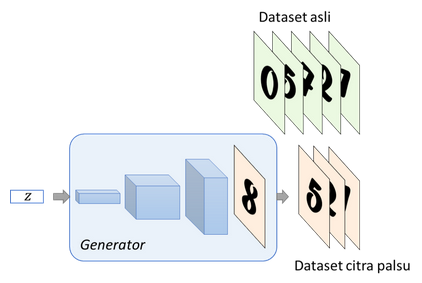
\includegraphics[width=6cm]{figures/1174006/chapter8/teori/1.png}
		\centering
    \end{figure}
    
	\item Jelaskan dengan ilustrasi gambar sendiri apa itu diskriminator dengan perumpamaan dosen anda sebagai diskriminatornya.\\
    
    Diskriminator merupakan jaringan yang mencoba membedakan antara data yang ada dengan data baru yang dihasilkan oleh generator.  Diskriminator mencoba memasukkan data inputan (data yang sudah ada) ke dalam kategori yang telah ditentukan. Perumpamaannya dosen atau dikriminator mencoba membedakan kodingan yang dibuat oleh saya dengan teman saya untuk menemukan kodingan yang mana yang sudah ada dan kodingan yang hasil perubahan.

    \begin{figure}[H]
        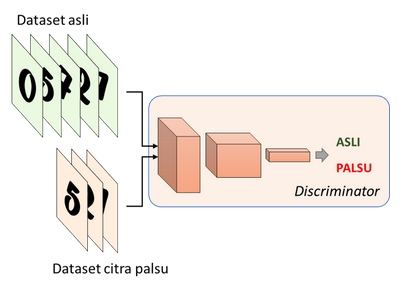
\includegraphics[width=6cm]{figures/1174006/chapter8/teori/2.png}
       \centering
   \end{figure}

	\item Jelaskan dengan ilustrasi gambar sendiri bagaimana arsitektur generator dibuat.\\
    Arsitektur generator:
    \begin{enumerate}
        \item Jaringan generator mencoba membuat data yang terlihat seperti data yang nyata dari data yang sudah ada.
        \item Ulangi langkah pertama hingga beberapa iterasi untuk mengecoh diskriminator dengan membuat data yang senyata mungkin.
        \item Hingga akhirnya, diskriminator melatih generator hingga ia tidak bisa lagi membedakan data nyata dan data yang palsu.
    \end{enumerate}

    \begin{figure}[H]
        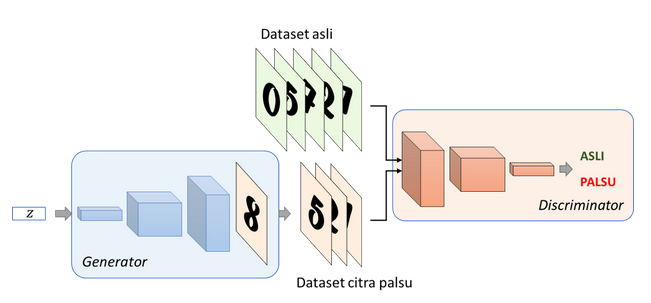
\includegraphics[width=6cm]{figures/1174006/chapter8/teori/3.PNG}
       \centering
   \end{figure}

	\item Jelaskan dengan ilustrasi gambar sendiri bagaimana arsitektur diskriminator
    dibuat.

    Arsitektur diskriminator:
    \begin{enumerate}
        \item Jaringan diskriminator mencoba mengidentifikasi apakah data tersebut asli atau palsu.
        \item Ulangi langkah pertama hingga beberapa iterasi untuk mengecoh generator dengan memperbaiki kriterianya untuk menentukan palsu tidaknya.
        \item Hingga akhirnya, diskriminator melatih generator hingga ia tidak bisa lagi membedakan data nyata dan data yang palsu.
    \end{enumerate}

    \begin{figure}[H]
        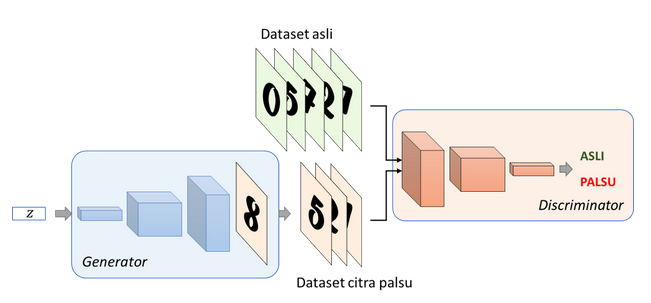
\includegraphics[width=6cm]{figures/1174006/chapter8/teori/3.PNG}
       \centering
   \end{figure}

    \item Jelaskan dengan ilustrasi gambar apa itu latent space.\\
    Latent space adalah data yang dibuat dari beberapa vektor secara acak.
    \begin{figure}[H]
        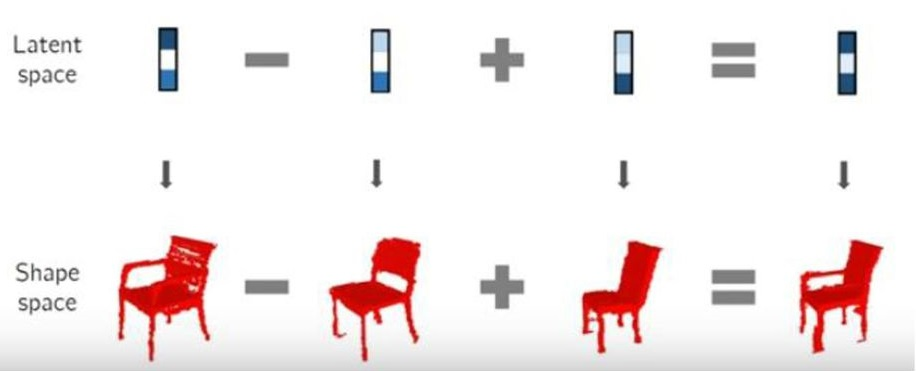
\includegraphics[width=6cm]{figures/1174006/chapter8/teori/4.jpg}
       \centering
   \end{figure}
    \item Jelaskan dengan ilustrasi gambar apa itu adversarial play.\\
    Adversarial play adalah proses pelatihan dimana jaringan discriminator dan jaringan generator berusaha saling memebodohi satu sama lain.
    
    \item Jelaskan dengan ilustrasi gambar apa itu Nash equilibrium.\\
    Nash Equilibrium adalah keadaan dimana jaringan discriminator tidak dapat membedakan lagi data asli dan data palsu.
    
    \item Sebutkan dan jelaskan contoh-contoh implementasi dari GAN.
    
    \begin{enumerate}
    	\item Image Generation, dimana GAN digunakan untuk mengenerate data baru dari perpaduan data asli yang ada.
    	\item Text to image synthesis, dimana GAN digunakan untuk mengenerate gambar berdasarkan deskripsi teks yang ada.
		\item Face aging, dimana GAN digunakan untuk mengenerate beberapa gambar wajah berbeda usia.
    	\item Image to image translation, dimana GAN digunakan untuk mengenerate gambar baru dari gambar yang sudah ada disertai dengan penambahan style.
		\item Video synthesis, dimana GAN digunakan untuk mengenerate sebuah video.
    	\item High resolution image generation, dimana GAN digunakan untuk meningkatkan resolusi atau mempertajam gambar.
    	\item Completing missing parts of images, dimana GAN digunakan untuk menambal bagian gambar yang hilang.
    \end{enumerate}
    
    
    \item Berikan contoh dengan penjelasan kode program beserta gambar arsitektur untuk membuat generator(neural network) dengan sebuah input layer, tiga hidden layer(dense layer), dan satu output layer(reshape layer).\\ \\
    Input Layer\\
    Pada input layer diambil sampel vertor 100 dimensi dan dilempar ke hidden layer pertama berupa tensor.\\
    \begin{lstlisting}
    input_shape=(batch_size, 100), output_shape=(batch_size, 100)
    \end{lstlisting}
    Hidden Layer\\
    Pada hidden layer akan ada proses konversi dari tensor yang dilempar dari layer sebelumnya. Pada hidden layer terdiri dari beberpa dense layer dengan beberapa unit juga.\\
    \begin{lstlisting}
    neurons=500, input_shape=(batch_size, 100), output_shape=(batch_size, 500)
    \end{lstlisting}
    \begin{lstlisting}
    neurons=500, input_shape=(batch_size, 500), output_shape=(batch_size, 500)
    \end{lstlisting}
    \begin{lstlisting}
    neurons=784, input_shape=(batch_size, 500), output_shape=(batch_size, 784)
    \end{lstlisting}
    Output Layer\\
    Pada output layer akan digenerate gambar yang memiliki bentuk 28 x 28 unit.\\
    \begin{lstlisting}
    input_shape=(batch_size, 784), output_shape=(batch_size, 28, 28)
    \end{lstlisting}
    \begin{figure}[H]
    	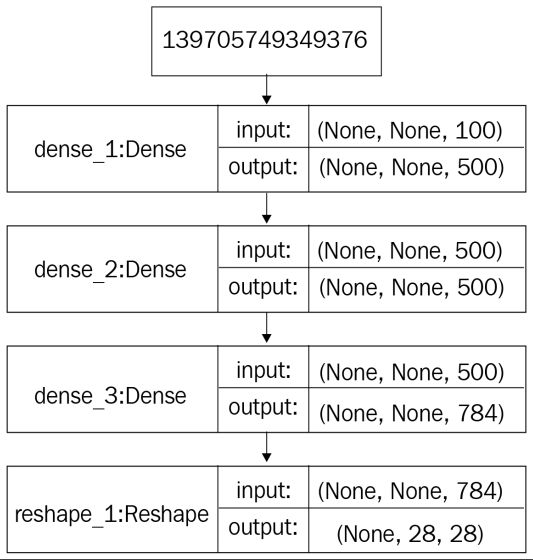
\includegraphics[width=6cm]{figures/1174006/chapter8/teori/arc.png}
    	\centering
    \end{figure}
    \item Berikan contoh dengan ilustrasi dari arsitektur dikriminator dengan sebuath input layer, 3 buah hidden layer, dan satu output layer.
    \begin{figure}[H]
    	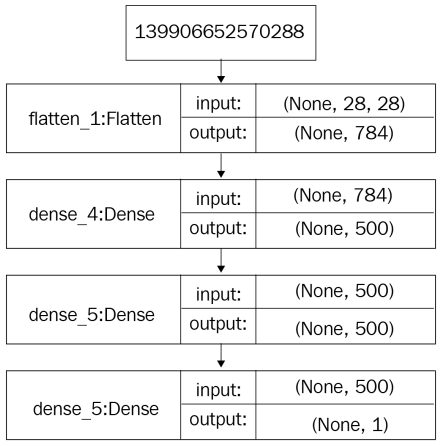
\includegraphics[width=6cm]{figures/1174006/chapter8/teori/arc2.png}
    	\centering
    \end{figure}
    \item Jelaskan bagaimana kaitan output dan input antara generator dan diskriminator tersebut. Jelaskan kenapa inputan dan outputan seperti itu.\\
    Inputan pada jaringan generator akan menerima input dari gambar asli, kemudian akan diolah oleh jaringan generator untuk dibuatkan gambar palsunya. Setelah dibuat gambar palsunya, kemudian akan diolah oleh jaringan diskriminator untuk dibedakan apakah gambar yang diolah sebelumnya oleh jaringan generator adalah asli atau palsu. Setelah diolah oleh jaringan discriminator akan mengembalikan value 0 atau 1
    
    \item Jelaskan apa perbedaan antara Kullback-Leibler divergence (KL divergence)/relative entropy, Jensen-Shannon(JS) divergence / information radius(iRaD) / total divergence to the average dalam mengukur kualitas dari model.\\
    Kullback-Leibler divergence tidak menerapkan symmetric nature untuk mengukur jarak antara dua probabilitas distribusi, sedangkan Jensen-Shannon divergence menerapkan symmetric nature.
    
    
    \item Jelaskan apa itu fungsi objektif yang berfungsi untuk mengukur kesamaan antara gambar yang dibuat dengan yang asli.\\
    Fungsi objektif berfungsi untuk mengukur kesamaan antara gambar yang dibuat dengan yang asli.
    
    \item Jelaskan apa itu scoring algoritma selain mean square error atau cross entropy seperti The Inception Score dan The Frechet Inception distance.\\
    Scoring algoritma adalah algoritma yang digunakan untuk menghitung akurasi GAN.
    
    \item Jelaskan kelebihan dan kekurangan GAN.\\
    Kelebihan
    \begin{enumerate}
    	\item Data hasil generate GAN terlihat mirip dengan data asli.
		\item Gampang dalam mengenali suatu objek dan bisa menghitung jarak antar objek
    \end{enumerate}
    Kekurangan
    \begin{enumerate}
    	\item Susah untuk dilatih
    \end{enumerate}

\end{enumerate}

\subsection{Praktek}
\begin{enumerate}
	\item Jelaskan apa itu 3D convolutions\\
	3D convolution adalah operasi menerapkan filter 3D ke data input sepanjang tiga arah, yaitu x, y, z. Operasi akan membuat daftar 3D fitur secara bertumpuk, outputnya nanti berupa kotak.
	
	\item Jelaskan dengan kode program arsitektur dari generator networknya, beserta penjelasan input dan output dari generator network.
	\\ \\
	Input Layer\\
	Pada input layer diambil sampel vertor 100 dimensi dan dilempar ke hidden layer pertama berupa tensor.\\
	\begin{lstlisting}
	input_shape=(batch_size, 100), output_shape=(batch_size, 100)
	\end{lstlisting}
	Hidden Layer\\
	Pada hidden layer akan ada proses konversi dari tensor yang dilempar dari layer sebelumnya. Pada hidden layer terdiri dari beberpa dense layer dengan beberapa unit juga.\\
	\begin{lstlisting}
	neurons=500, input_shape=(batch_size, 100), output_shape=(batch_size, 500)
	\end{lstlisting}
	\begin{lstlisting}
	neurons=500, input_shape=(batch_size, 500), output_shape=(batch_size, 500)
	\end{lstlisting}
	\begin{lstlisting}
	neurons=784, input_shape=(batch_size, 500), output_shape=(batch_size, 784)
	\end{lstlisting}
	Output Layer\\
	Pada output layer akan digenerate gambar yang memiliki bentuk 28 x 28 unit.\\
	\begin{lstlisting}
	input_shape=(batch_size, 784), output_shape=(batch_size, 28, 28)
	\end{lstlisting}
	\begin{figure}[H]
		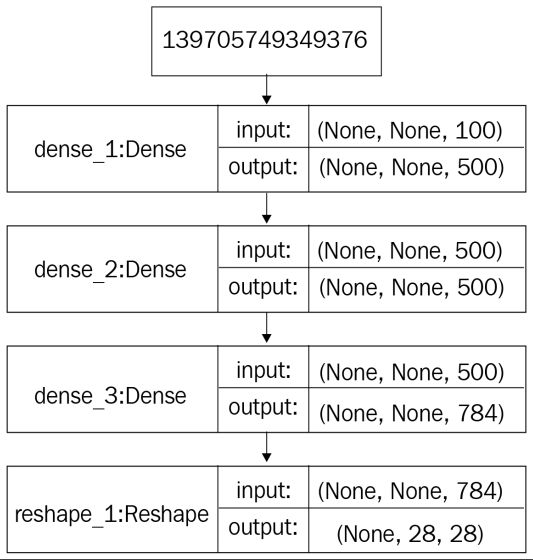
\includegraphics[width=6cm]{figures/1174006/chapter8/teori/arc.png}
		\centering
	\end{figure}

	\item Jelaskan dengan kode program arsitektur dari diskriminator network, beserta penjelasan input dan outputnya.
	\\ \\
	Input Layer\\
	Pada input layer diambil sampel vertor 100 dimensi dan dilempar ke hidden layer pertama berupa tensor.\\
	\begin{lstlisting}
	input_shape=(batch_size, 100), output_shape=(batch_size, 100)
	\end{lstlisting}
	Hidden Layer\\
	Pada hidden layer akan ada proses konversi dari tensor yang dilempar dari layer sebelumnya. Pada hidden layer terdiri dari beberpa dense layer dengan beberapa unit juga.\\
	Pertama dicriminator akan menerima inputan bentuk 28 x 28. Lalu diteruskan ke hidden layer tanpa dimodifikasi. Pada hidden layer akan dimodifikasi. Lalu pada layer terakhir atau output layer ditentukan apakah data tadi adalah asli atau palsu
	\begin{figure}[H]
		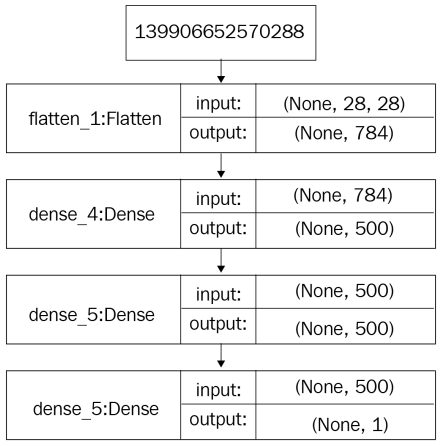
\includegraphics[width=6cm]{figures/1174006/chapter8/teori/arc2.png}
		\centering
	\end{figure}
	\item Jelaskan proses training 3D-GANs.
	\begin{enumerate}
		\item Siapkan sample 200 dimensi berbentuk vektor.
		\item Generate sebuah gambar palsu dengan model generator.
		\item Latih jaringan generator dengan gambar asli dan gambar palsu.
		\item Gunakan adversial model untuk melatih generator model.
		\item Ulangi langkah diatas sampai epoch tertentu.
		
	\end{enumerate}
	\item Jelaskan bagaimana melakukan settingan awal chapter 02 untuk memenuhi semua kebutuhan sebelum melanjutkan ke tahapan persiapan data.
	\begin{enumerate}
		\item Download terlebih dahulu data yang akan diolah
		\item Siapkan IDE yang akan dipakai untuk mengolah data.
		\item Panggil data yang telah didownload tadi.
	\end{enumerate}
	\item Jelaskan tentang dataset yang digunakan, dari mulai tempat unduh, cara membuka dan melihat data. Sampai deskripsi dari isi dataset dengan detail penjelasan setiap folder/file yang membuat orang awam paham.
	\begin{enumerate}
		\item Pertama download dataset dengan mengetik wget http://3dshapenets.cs.princeton.edu/3DShapeNetsCode.zip
		\item Lalu extract dataset tadi dengan mengetik unzip 3DShapeNetsCode.zip
		\item Panggil data yang telah didownload tadi.
	\end{enumerate}
	\item Jelaskan apa itu voxel dengan ilustrasi dan bahasa paling awam.\\
	Voxel adalah point pada bentuk 3 dimesional, biasanya berup posisi dari 3 koordinat yaitu x, y, dan z.
	
	\item Visualisasikan dataset tersebut dalam tampilan visual plot, jelaskan cara melakukan visualisasinya.
	\begin{enumerate}
		\item Pertama load data gambar 3D.
		\item Lalu visualisasikan data gambar 3D tadi.
	\end{enumerate}
	\begin{figure}[H]
		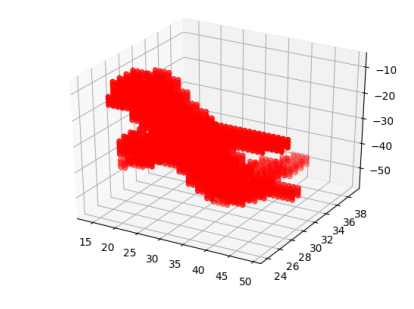
\includegraphics[width=6cm]{figures/1174006/chapter8/praktek/ex.png}
		\centering
	\end{figure}
	
	\item Buka file run.py jelaskan perbaris kode pada fungsi untuk membuat generator yaitu build generator.\\
	Pada kode fungsi build\_generator() dibuat untuk nantinya dipakai sebagai model generator. Di fungsi tersebut berisikan layer-layer yang terla di definisikan sesuai keperluan generator.
	
	\item Jelaskan juga fungsi untuk membangun diskriminator pada fungsi build discriminator.\\
	Pada kode fungsi build\_discriminator() dibuat untuk nantinya dipakai sebagai model discriminator. Di fungsi tersebut berisikan layer-layer yang terla di definisikan sesuai keperluan discriminator.
	
	\item Jelaskan apa maksud dari kode program \_\_name\_\_ == '\_\_main\_\_'
    \begin{lstlisting}[caption=Kode program utama,label={lst:8.1}]
    if __name__ == '__main__':
    \end{lstlisting}
    Kode program tersebut untuk mengecek apakah module yang dipakai adalah main.
    
    \item Jelaskan secara detil perbaris dan per parameter apa arti dari kode program :
    \begin{lstlisting}[caption=Setting Parameter,label={lst:8.2}]
        object_name = "chair"
        data_dir = "data/3DShapeNets/volumetric_data/" \
                "{}/30/train/*.mat".format(object_name)
        gen_learning_rate = 0.0025
        dis_learning_rate = 10e-5
        beta = 0.5
        batch_size = 1
        z_size = 200
        epochs = 10
    \end{lstlisting}
    Kode program diatas tentang mendefinisikan variable yang akan dipakai.
    
    \item Jelaskan secara detil dari kode program pembuatan dan kompilasi arsitektur berikut :
    \begin{lstlisting}[caption=Setting Parameter,label={lst:8.2}]
        gen_optimizer = Adam(lr=gen_learning_rate, beta_1=beta)
        dis_optimizer = Adam(lr=dis_learning_rate, beta_1=beta)

        discriminator = build_discriminator()
        discriminator.compile(loss='binary_crossentropy', optimizer=dis_optimizer)

        generator = build_generator()
        generator.compile(loss='binary_crossentropy', optimizer=gen_optimizer)
    \end{lstlisting}
    Kode program diatas tentang pembuatan dan kompilasi model generator dan discriminator yang nantinya dipakai.
    
    \item Jelaskan secara detil kode program untuk membuat dan melakukan kompilasi model adversarial berikut:
    \begin{lstlisting}[caption=Membuat dan Kompilasi Model Adversarial,label={lst:8.3}]
        discriminator.trainable = False

        input_layer = Input(shape=(1, 1, 1, z_size))
        generated_volumes = generator(input_layer)
        validity = discriminator(generated_volumes)
        adversarial_model = Model(inputs=[input_layer], outputs=[validity])
        adversarial_model.compile(loss='binary_crossentropy', optimizer=gen_optimizer)
    \end{lstlisting}
    Kode program diatas tentang pembuatan dan kompilasi model adversial yang nantinya dipakai.
    
    \item Jelaskan Ekstrak dan load data kursi dengan menggunakan fungsi getVoxelsFormat dan get3DImages yang digunakan pada kode program berikut :
    \begin{lstlisting}[caption=Ekstraksi dan load dataset,label={lst:8.4}]
        print("Loading data...")
        volumes = get3DImages(data_dir=data_dir)
        volumes = volumes[..., np.newaxis].astype(np.float)
        print("Data loaded...")
    \end{lstlisting}
    Kode program diatas tentang meload data gambar 3D.
    
    \item Jelaskan maksud dari kode program instansiasi TensorBoard yang menambahkan generator dan diskriminator pada program berikut:
    \begin{lstlisting}[caption=Instansiasi tensorboard,label={lst:8.5}]
        tensorboard = TensorBoard(log_dir="logs/{}".format(time.time()))
        tensorboard.set_model(generator)
        tensorboard.set_model(discriminator)
    \end{lstlisting}
    Kode program diatas tentang mengevaluasi model yang dibuat dengan menggunakan TensorBoard.
    
    \item Jelaskan apa fungsi dari np reshape ones zeros pada kode program berikut dengan parameternya:
    \begin{lstlisting}[caption=Pelabelan dataset,label={lst:8.6}]
        labels_real = np.reshape(np.ones((batch_size,)), (-1, 1, 1, 1, 1))
        labels_fake = np.reshape(np.zeros((batch_size,)), (-1, 1, 1, 1, 1))
    \end{lstlisting}
    Kode program diatas tentang pelabelan data asli dan palsu.
    
    \item Jelaskan kenapa harus ada perulangan dalam meraih epoch. Dan jelaskan apa itu epoch terkait kode program berikut:
    \begin{lstlisting}[caption=Setting Epoch,label={lst:8.7}]
            for epoch in range(epochs):
                print("Epoch:", epoch)

                gen_losses = []
                dis_losses = []
    \end{lstlisting}
    Epoch dilakukan untuk mendapat hasil yang akurat. Kode program diatas tentang menampung tinggkat loss dari generator dan discriminator.
    
    \item Jelaskan apa itu batches dan kaitannya dengan kode program berikut, dan kenapa berada di dalam epoch:
    \begin{lstlisting}[caption=Setting Batch,label={lst:8.8}]
                number_of_batches = int(volumes.shape[0] / batch_size)
                print("Number of batches:", number_of_batches)
                for index in range(number_of_batches):
                    print("Batch:", index + 1)
    \end{lstlisting}
    Batch dipakai terkait pembagian proses pada tiap epoch yang dilakukan.
    
    \item Berikut adalah kode program pengambilan gambar dan noise. Jelaskan apa fungsi np.random.normal serta astype, serta jelaskan apa arti parameter titik dua dan jelaskan isi dari z\_sample dan volumes\_batch:
    \begin{lstlisting}[caption=Set real images dan vektor noise,label={lst:8.9}]
                    z_sample = np.random.normal(0, 0.33, size=[batch_size, 1, 1, 1, z_size]).astype(np.float32)
                    volumes_batch = volumes[index * batch_size:(index + 1) * batch_size, :, :, :]
    \end{lstlisting}

    \item Berikut adalah kode program generator gambar palsu. Jelaskan apa fungsi generator.predict\_on\_batch, serta jelaskan apa arti parameter z\_sample:
    \begin{lstlisting}[caption=Generator Gambar Palsu,label={lst:8.10}]
                    # Next, generate volumes using the generate network
                    gen_volumes = generator.predict_on_batch(z_sample)
    \end{lstlisting}

    \item Berikut adalah kode program training diskriminator dengan gambar palsu dari generator dan gambar asil. Jelaskan apa maksudnya harus dilakukan training diskriminator secara demikian dan jelaskan apa isi loss\_fake dan loss\_real serta d\_loss dan fungsi train\_on\_batch.
    \begin{lstlisting}[caption=Training Diskriminator,label={lst:8.11}]
                    discriminator.trainable = True
                    if index % 2 == 0:
                        loss_real = discriminator.train_on_batch(volumes_batch, labels_real)
                        loss_fake = discriminator.train_on_batch(gen_volumes, labels_fake)

                        d_loss = 0.5 * np.add(loss_real, loss_fake)
                        print("d_loss:{}".format(d_loss))

                    else:
                        d_loss = 0.0
    \end{lstlisting}

    \item Berikut adalah kode program training model adversarial yang terdapat generator dan diskriminator. Jelaskan apa bagaimana proses terbentuknya parameter z dan g\_loss:
    \begin{lstlisting}[caption=Training adversarial model,label={lst:8.12}]
                    z = np.random.normal(0, 0.33, size=[batch_size, 1, 1, 1, z_size]).astype(np.float32)
                    g_loss = adversarial_model.train_on_batch(z, labels_real)
                    print("g_loss:{}".format(g_loss))

                    gen_losses.append(g_loss)
                    dis_losses.append(d_loss)
    \end{lstlisting}

    \item Berikut adalah kode program generate dan menyimpan gambar 3D setelah beberapa saat setiap epoch. Jelaskan mengapa ada perulangan dengan parameter tersebut, serta jelaskan arti setiap variabel beserta perlihatkan isinya dan artikan isinya :
    \begin{lstlisting}[caption=Buat dan simpan gambar 3D,label={lst:8.13}]
                    # Every 10th mini-batch, generate volumes and save them
                    if index % 10 == 0:
                        z_sample2 = np.random.normal(0, 0.33, size=[batch_size, 1, 1, 1, z_size]).astype(np.float32)
                        generated_volumes = generator.predict(z_sample2, verbose=3)
                        for i, generated_volume in enumerate(generated_volumes[:5]):
                            voxels = np.squeeze(generated_volume)
                            voxels[voxels < 0.5] = 0.
                            voxels[voxels >= 0.5] = 1.
                            saveFromVoxels(voxels, "results/img_{}_{}_{}".format(epoch, index, i))
    \end{lstlisting}

    \item Berikut adalah kode program menyimpan average losses setiap epoch. Jelaskan apa itu tensorboard dan setiap parameter yang digunakan pada kode program ini :
    \begin{lstlisting}[caption=Simpan Average losses setiap epoch,label={lst:8.14}]
                # Write losses to Tensorboard
                write_log(tensorboard, 'g_loss', np.mean(gen_losses), epoch)
                write_log(tensorboard, 'd_loss', np.mean(dis_losses), epoch)
    \end{lstlisting}

    \item Berikut adalah kode program menyimpan model. Jelaskan apa itu format h5 dan penjelasan dari kode program berikut :
    \begin{lstlisting}[caption=Simpan model,label={lst:8.15}]
            generator.save_weights(os.path.join("models", "generator_weights.h5"))
            discriminator.save_weights(os.path.join("models", "discriminator_weights.h5"))
    \end{lstlisting}

    \item Berikut adalah kode program testing model. Jelaskan dengan ilustrasi gambar dari mulai meload hingga membuat gambar 3D dengan menggunakan z\_sample, bisakah parameter z\_sample tersebut diubah2? :
    \begin{lstlisting}[caption=Testing model,label={lst:8.16}]
            # Create models
            generator = build_generator()
            discriminator = build_discriminator()

            # Load model weights
            generator.load_weights(os.path.join("models", "generator_weights.h5"), True)
            discriminator.load_weights(os.path.join("models", "discriminator_weights.h5"), True)

            # Generate 3D models
            z_sample = np.random.normal(0, 1, size=[batch_size, 1, 1, 1, z_size]).astype(np.float32)
            generated_volumes = generator.predict(z_sample, verbose=3)

            for i, generated_volume in enumerate(generated_volumes[:2]):
                voxels = np.squeeze(generated_volume)
                voxels[voxels < 0.5] = 0.
                voxels[voxels >= 0.5] = 1.
                saveFromVoxels(voxels, "results/gen_{}".format(i))
    \end{lstlisting}
    
\end{enumerate}

\subsection{Penanganan Error}
\begin{enumerate}
	\item Screenshoot Error
	\item Tuliskan kode eror dan jenis errornya
	\item Solusi pemecahan masalah error tersebut
    
\end{enumerate}
%\input{chapters/chapter1/1174027}
%\section{1174031 - Muhammad Tomy Nur Maulidy}
\subsection{Soal Teori}
\begin{enumerate}

	\item Jelaskan dengan ilustrasi gambar sendiri apa itu generator dengan perumpamaan anda sebagai mahasiswa sebagai generatornya.
	\hfill\break
	Tugas Generator sekarang sedang dibuat untuk membuat koleksi gambar palsu, yang saat ini dilihat oleh Diskriminator. Diskriminator tidak dapat membedakan antara yang asli dan yang palsu. Untuk ilustrasi, lihat gambar berikut: 

	\begin{figure}[H]
	\centering
		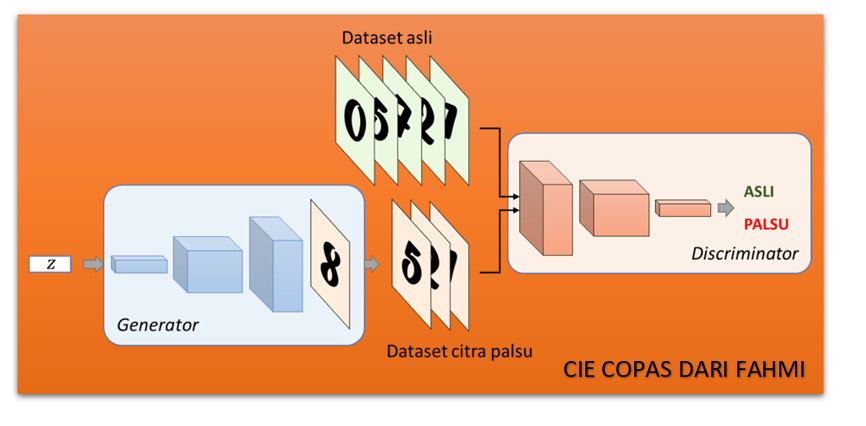
\includegraphics[width=4cm]{figures/1174031/8/teori1,2.PNG}
		\caption{Teori 1}
	\end{figure}

	\item Jelaskan dengan ilustrasi gambar sendiri apa itu diskriminator dengan perumpamaan dosen anda sebagai diskriminatornya.

	\hfill\break
	Diskriminator adalah CNN yang menerima input gambar yang dimiliki dan menghasilkan angka biner yang meminta input gambar, lalu menghasilkan gambar dari dataset asli atau menghasilkan gambar palsu. Untuk ilustrasi, lihat gambar berikut: 

	\begin{figure}[H]
	\centering
		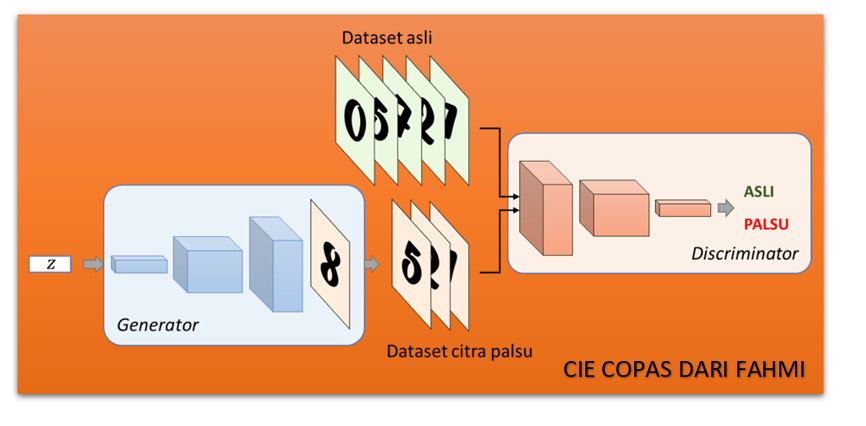
\includegraphics[width=4cm]{figures/1174031/8/teori1,2.PNG}
		\caption{Teori 2}
	\end{figure}
	
	\item Jelaskan dengan ilustrasi gambar sendiri bagaimana arsitektur generator dibuat.

	\hfill\break
	Aksitektur generator dibuat bisa dijelaskan pada gambar berikut : 

	\begin{figure}[H]
	\centering
		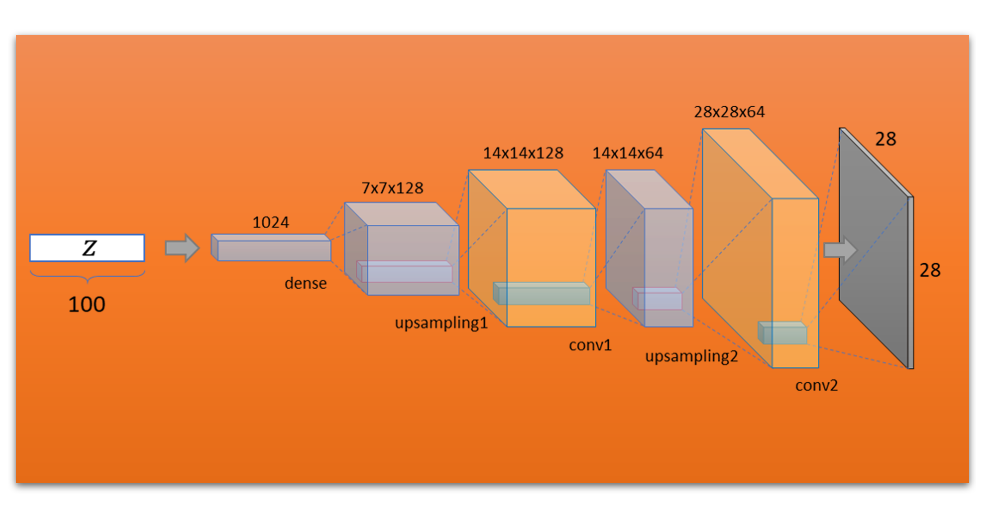
\includegraphics[width=4cm]{figures/1174031/8/teori3.PNG}
		\caption{Teori 3}
	\end{figure}

	\item Jelaskan dengan ilustrasi gambar sendiri bagaimana arsitektur diskriminator dibuat.

	\hfill\break
	Aksitektur diskriminator dibuat bisa dijelaskan pada gambar berikut : 

	\begin{figure}[H]
	\centering
		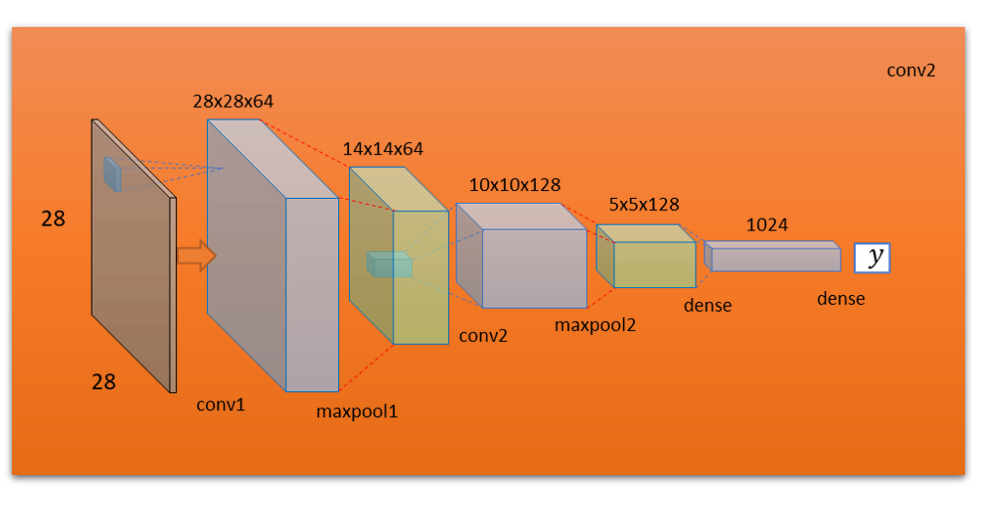
\includegraphics[width=4cm]{figures/1174031/8/teori4.PNG}
		\caption{Teori 4}
	\end{figure}

	\item Jelaskan dengan ilustrasi gambar apa itu latent space.
	\hfill\break
	Latent space dijelaskan pada gambar berikut : 

	\begin{figure}[H]
	\centering
		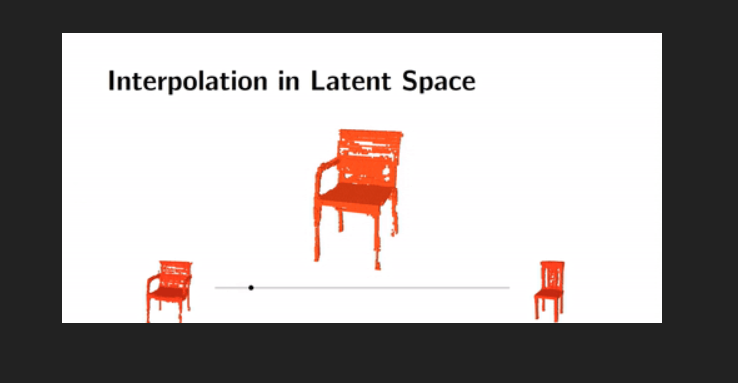
\includegraphics[width=4cm]{figures/1174031/8/teori5.PNG}
		\caption{Teori 5}
	\end{figure}

	\item Jelaskan dengan ilustrasi gambar apa itu adversarial play.
	\hfill\break
	Adversarial play dijelaskan pada gambar berikut : 

	\begin{figure}[H]
	\centering
		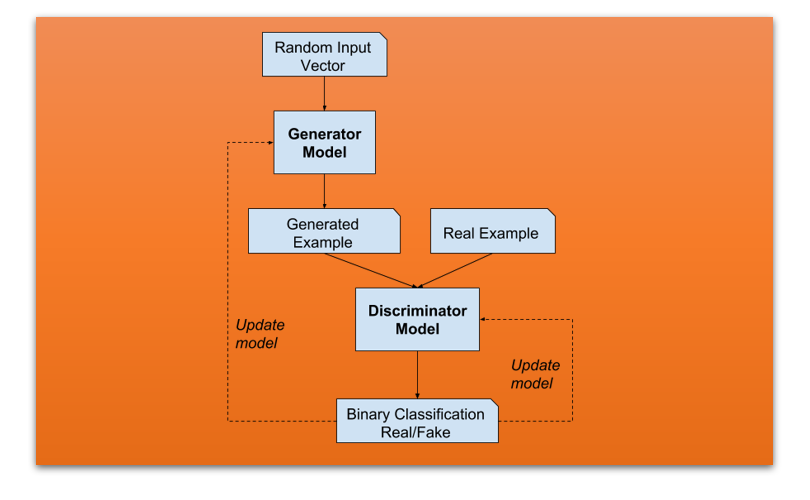
\includegraphics[width=4cm]{figures/1174031/8/teori6.PNG}
		\caption{Teori 6}
	\end{figure}

	\item Jelaskan dengan ilustrasi gambar apa itu Nash equilibrium.
	\hfill\break
	Nash equilibrium adalah Teori permainan adalah studi tentang interaksi strategis antara agen rasional. Sederhananya itu berarti itu adalah studi interaksi ketika pihak-pihak yang terlibat mencoba dan melakukan yang terbaik dari sudut pandang mereka, detailnya dapat dijelaskan pada gambar berikut : 

	\begin{figure}[H]
	\centering
		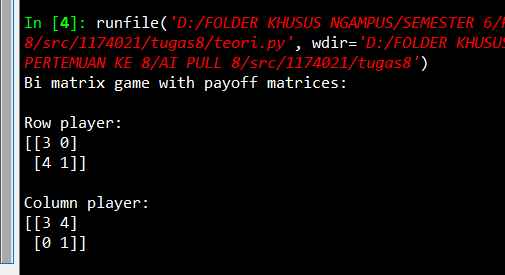
\includegraphics[width=4cm]{figures/1174031/8/teori7.PNG}
		\caption{Teori 7}
	\end{figure}

	\item Sebutkan dan jelaskan contoh-contoh implementasi dari GAN.

	\hfill\break
	Menurut saya implementasi 3DGAN yaitu pada MAPS dan juga IKEA. Karena pada maps dan juga ikea sudah menerapkan bentuk 3 dimensi yang bisa lebih menarik perhatikan pengguna.

	\item Berikan contoh dengan penjelasan kode program beserta gambar arsitektur untuk membuat generator(neural network) dengan sebuah input layer, tiga hidden layer(dense layer), dan satu output layer(reshape layer).
	\hfill\break

	Untuk penjelasan tersebut dijelaskan pada gambar dibawah ini :

	\begin{figure}[H]
	\centering
		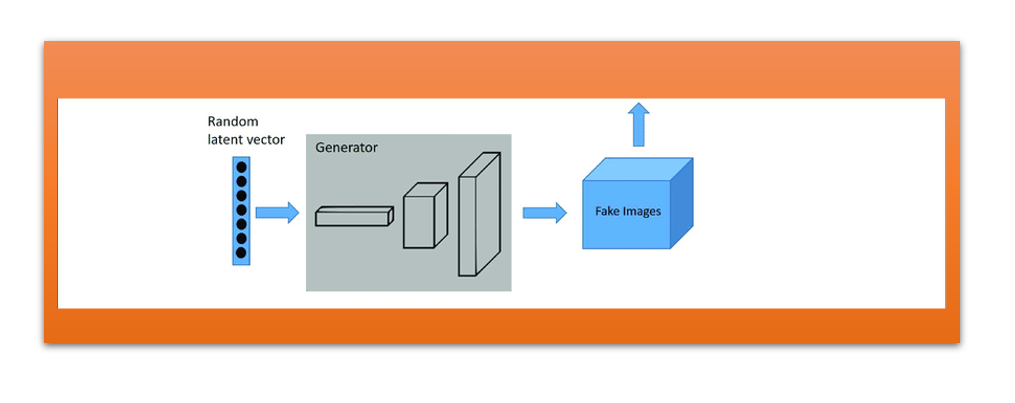
\includegraphics[width=4cm]{figures/1174031/8/teori9.PNG}
		\caption{Teori 9}
	\end{figure}

	\item Berikan contoh dengan ilustrasi dari arsitektur dikriminator dengan sebuath input layer, 3 buah hidden layer, dan satu output layer.
	\hfill\break

	Untuk penjelasan tersebut dijelaskan pada gambar dibawah ini :

	\begin{figure}[H]
	\centering
		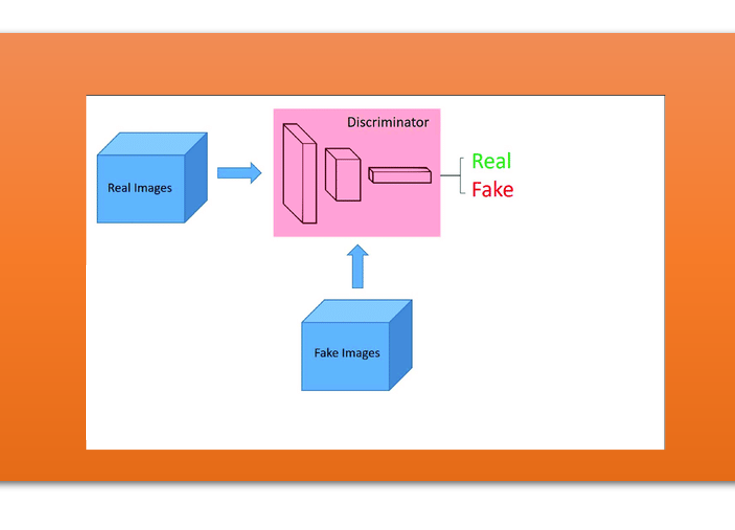
\includegraphics[width=4cm]{figures/1174031/8/teori10.PNG}
		\caption{Teori 10}
	\end{figure}

	\item Jelaskan bagaimana kaitan output dan input antara generator dan diskriminator tersebut. Jelaskan kenapa inputan dan outputan seperti itu.
	\hfill\break

	Gambar dari Generator yang berhasil di deteksi oleh Diskriminator sebagai gambar fake, akan dikembalikan dengan feedback pke generator. Kini Generator bertugas untuk bisa membuat sekumpulan gambar palsu, yang nantinya dapat dilihat oleh Diskriminator, lalu, Diskriminator tidak bisa membedakan fake dan real.

	\item Jelaskan apa perbedaan antara Kullback-Leibler divergence (KL divergence)/relativeentropy, Jensen-Shannon(JS) divergence / information radius(iRaD) / total divergence to the average dalam mengukur kualitas dari model.
	\hfill\break

	Perbedaan nya yaitu memiliki model dari rumus yang berbeda-beda sehingga mempengaruhi hasil train dan test

	\item Jelaskan apa itu fungsi objektif yang berfungsi untuk mengukur kesamaan antara gambar yang dibuat dengan yang asli.
	\hfill\break

	Ukuran penting untuk menilai kualitas model. lalu kemudian akan melihat di keseimbangan Nash.

	\item Jelaskan apa itu scoring algoritma selain mean square error atau cross entropy seperti The Inception Score dan The Frechet Inception distance.
	\hfill\break

	The inception score adalah algoritma penilaian yang paling banyak digunakan untuk GAN. The Frechet Inception distance adalah Untuk mengatasi berbagai kekurangan Skor awal

	\item Jelaskan kelebihan dan kekurangan GAN.
	\hfill\break

	Kelebihan : GAN dapat memvisualiasikan bentuk model menjadi plot. Kemudian pada Kelemahan : model susah untuk implementasikan yang membuat data training menjadi lemah.

\end{enumerate}

\subsection{Praktek Program}
\begin{enumerate}
	\item Soal 1
	\hfill\break

	Konvolusi 3D. Konvolusi 3D menerapkan filter 3 dimensi ke kumpulan data dan filter 3 arah (x, y, z) untuk menghitung representasi fitur tingkat rendah. Bentuk outputnya adalah ruang volume 3 seperti kubus atau berbentuk kubus. 3D sangat membantu dalam pendeteksian peristiwa dalam video, gambar medis 3D, dll. Generative Adversarial Network adalah arsitektur jaringan saraf tiruan yang dimaksudkan untuk membuat atau membuat data yang benar-benar baru, dari nol hingga tidak ada sama sekali. Melihat target utama GAN adalah data gambar. Singkatnya, jaringan GAN berfungsi untuk memberikan gambar baru berdasarkan koleksi gambar yang telah ada sebelumnya selama proses training.

	\item Soal 2
	\hfill\break
	\lstinputlisting[firstline=31, lastline=61]{src/1174031/8/run.py}
	Kode di atas akan melakukan create generator ialah gloss, Bentuk jaringan Generator dapat dilihat berkebalikan dengan struktur jaringan saraf pada umumnya. Generator biasanya menerima input sebuah vektor z, yang kemudian mengubahnya menjadi sebuah output 3D atau 3 dimensi.

	\item Soal 3
	\hfill\break
	\lstinputlisting[firstline=66, lastline=104]{src/1174031/8/run.py}
	Diskrimanator adalah d\_loss, Jaringan Discriminator merupakan jaringan klasifikasi biner yang menerima input gambar tiga dimensi dan mengeluarkan klasifikasi menyatakan input gambar adalah gambar asli dari dataset atau merupakan gambar buatan Generator. Diskriminator dilatih dengan dataset yang diambil dari Generator, lalu di training untuk membedakan keduanya. Gambar dari Generator yang berhasil di deteksi oleh Diskriminator sebagai gambar fake, akan dikembalikan dengan feedback pke generator. Kini Generator bertugas untuk bisa membuat sekumpulan gambar palsu, yang nantinya dapat dilihat oleh Diskriminator, lalu, Diskriminator tidak bisa membedakan fake dan real.

	\item Soal 4
	\hfill\break
	Proses training 3D GAN yaitu dengan melakukan epoch sebanyak yang ditentukan.

	\item Soal 5
	\hfill\break
	\begin{itemize}
		\item Clone github
		\item Download dataset
		\item Buat folder baru logs dan results
	\end{itemize}

	\item Soal 6
	\hfill\break
	Dataset yang digunakan yaitu 3DShapeNets yang berisi model model bentuk benda dll, folder train berisi train dan folder test berisi data testing. dan semua data tersebut di simpan didalam folder volumetric\_data.

	\item Soal 7
	\hfill\break
	Volume pixel atau voxel adalah titik dalam ruang tiga dimensi. Sebuah voxel mendefinisikan posisi dengan tiga koordinat dalam arah x, y, dan z. Sebuah voxel adalah unit dasar untuk mewakili gambar 3D. Untuk gambar nya ialah sebagai berikut :
	\begin{figure}[H]
	\centering
		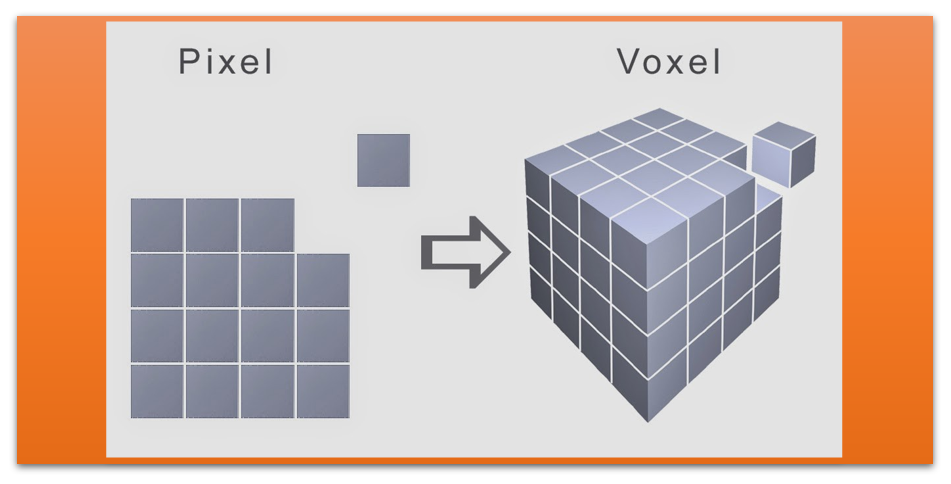
\includegraphics[width=4cm]{figures/1174031/8/praktek7.PNG}
		\caption{Praktek Soal 7}
	\end{figure}

	\item Soal 8
	\hfill\break
	\lstinputlisting[firstline=1, lastline=26]{src/1174031/8/display.py}
	Kode di atas befungsi untuk visualisasidataset dalam tampilan plot. langkah-langkah seperti ini :
	import library, load data file .mat dan lakukan read memakai matplotlib, Hasilnya adalah sebagai berikut :
	\begin{figure}[H]
	\centering
		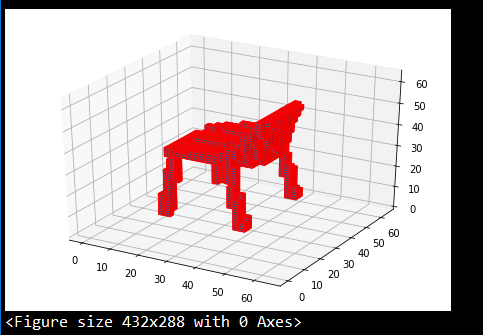
\includegraphics[width=4cm]{figures/1174031/8/praktek8.PNG}
		\caption{Hasil Soal 8}
	\end{figure}

	\item Soal 9
	\hfill\break
	\lstinputlisting[firstline=31, lastline=61]{src/1174031/8/run.py}
	Kode di atas befungsi untuk membuat generator yaitu dengan ketentukan gen sebagai variabel dan membuat fungsi atau variabel genmodel lalu dilakukan return. 
	
	\item Soal 10
	\hfill\break
	\lstinputlisting[firstline=66, lastline=104]{src/1174031/8/run.py}
	Kode di atas befungsi untuk membangun diskriminator berfungsi untuk mendefenisikan seluruh gambar yang sudah di load generator sebagai gambar fake dan real.

	\item Soal 11
	\hfill\break
	Jika interpreter python menjalankan if name == main sebagai program utama, itu ialah menetapkan variabel name untuk memiliki nilai main. Jika file ini sedang di impor dari modul lain, name akan ditetapkan ke nama modul. Nama modul tersedia sebagai nilai untuk name variabel global.

	\item Soal 12
	\hfill\break
	\lstinputlisting[firstline=162, lastline=171]{src/1174031/8/run.py}
	Kode di atas befungsi untuk melakukan load dataset dengan ketentuan data yang hanya dalam folder chair pada data train.

	\item Soal 13
	\hfill\break
	\lstinputlisting[firstline=174, lastline=184]{src/1174031/8/run.py}
	Kode di atas menggunakan Adam sebagai algoritma pengoptimalan dan binary\_crossentropy sebagai kerugian loss. 

	\item Soal 14
	\hfill\break
	\lstinputlisting[firstline=187, lastline=193]{src/1174031/8/run.py}
	Kode di atas artinya ialah kita memasukkan random vector kedalam generator model lalu membagi 2 yaitu generated example dan real example, dan meneruskan ke diskriminator model sebagai real atau fake

	\item Soal 15
	\hfill\break
	\lstinputlisting[firstline=196, lastline=199]{src/1174031/8/run.py}
	Kode di atas befungsi untuk melakukan load data pada dataset.

	\item Soal 16
	\hfill\break
	\lstinputlisting[firstline=202, lastline=204]{src/1174031/8/run.py}
	Kode di atas berfungsi untuk membuat tensorboard yang nantinya bisa diakses melalui localhost.

	\item Soal 17
	\hfill\break
	\lstinputlisting[firstline=207, lastline=208]{src/1174031/8/run.py}
	Kode di atas befungsi untuk melakukan reshape agar shape yang dihasilkan tidak terlalu besar. Dengan membuat variabel real dan fake.

	\item Soal 18
	\hfill\break
	\lstinputlisting[firstline=211, lastline=216]{src/1174031/8/run.py}
	Kode di atas befungsi untuk melakukan training epoch, karena jika epoch semakin banyak maka kualiatas training yang dihasilkan akan semakin baik.

	\item Soal 19
	\hfill\break
	\lstinputlisting[firstline=219, lastline=222]{src/1174031/8/run.py}
	Batch adalah jumlah file yang akan di training.

	\item Soal 20
	\hfill\break
	\lstinputlisting[firstline=225, lastline=226]{src/1174031/8/run.py}
	Kode di atas befungsi untuk untuk membuat gambar bersih dari noise dan juga menyesuaikan shape.

	\item Soal 21
	\hfill\break
	\lstinputlisting[firstline=229, lastline=234]{src/1174031/8/run.py}
	Kode di atas befungsi untuk membuat sample gambar palsu yang akan diteruskan ke diskriminator.

	\item Soal 22
	\hfill\break
	\lstinputlisting[firstline=237, lastline=246]{src/1174031/8/run.py}
	Kode di atas befungsi untuk membuat diskriminator bisa load gambar fake dan real dari generator, oleh karena itu ada generator loss dan diskriminator loss untuk melihat seberapa baik kualitas yang dihasilkan.

	\item Soal 23
	\hfill\break
	\lstinputlisting[firstline=249, lastline=258]{src/1174031/8/run.py}
	Kode di atas befungsi untuk melakukan print gloss untuk generator dan juga dloss untuk diskriminator.

	\item Soal 24
	\hfill\break
	\lstinputlisting[firstline=261, lastline=269]{src/1174031/8/run.py}
	Mengapa ada perulangan ? karena untuk melakukan perbandingan dari hasil yang sudah didapat.

	\item Soal 25
	\hfill\break
	\lstinputlisting[firstline=272, lastline=278]{src/1174031/8/run.py}
	TensorBoard adalah sebuah aplikasi web localhost untuk memeriksa dan menyelesaikan grafik dari hasil TensorFlow.

	\item Soal 26
	\hfill\break
	\lstinputlisting[firstline=281, lastline=282]{src/1174031/8/run.py}
	File H5 adalah file data yang disimpan dalam Format Data Hirarki (HDF). Ini berisi array multidimensi data ilmiah.

	\item Soal 27
	\hfill\break
	\lstinputlisting[firstline=285, lastline=302 ]{src/1174031/8/run.py}
	Ini adalah tahap akhir untuk melakukan testing dari model yang telah dibuat dan buat model dari yang sudah di create sebelumnya yaitu generator dan diskriminator. Untuk ilustrasi gambar sebagai berikut : 

	\begin{figure}[H]
	\centering
		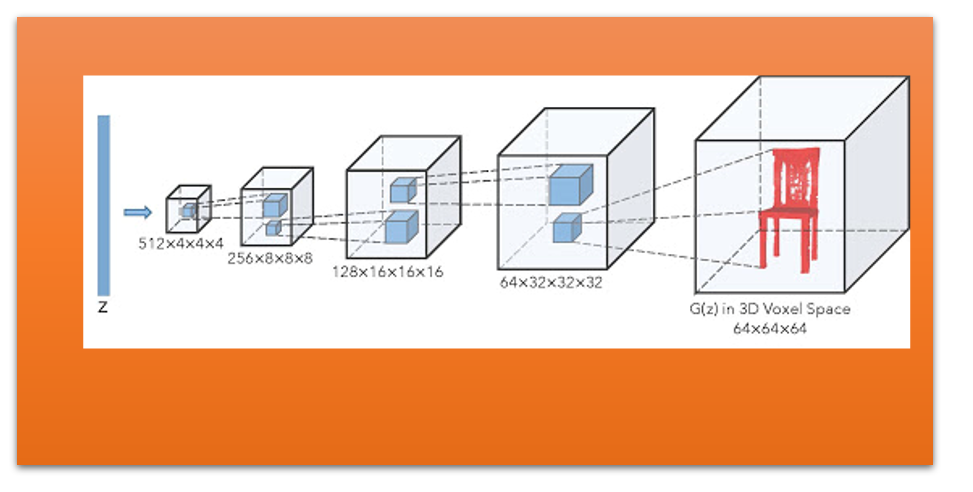
\includegraphics[width=4cm]{figures/1174031/8/praktek27.PNG}
		\caption{Praktek Soal 27}
	\end{figure}
\end{enumerate}


%\section{Dwi Septiani Tsaniyah/ 1174003}
\subsection{Teori}

\begin{enumerate}

\item Jelaskan kenapa file suara harus dilakukan MFCC dilengkapi dengan ilustrasi atau gambar.\par
Karena MFCCdigunakan untuk mengidentifikasi jenis suara misalkan jenis suara gendre lagu jes pop metal dan klasikal atau suara ultra sonic.
Sehingga dibutuhkan penggunaan MFCC untuk memproses data tersebut agar dapat dibaca oleh manusia.

\begin{figure}[ht]
\centering
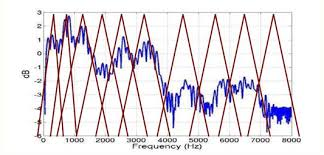
\includegraphics[scale=0.5]{figures/1174003/chapter6/1,1.jpg}
\caption{Ilustrasi gambar metode MFCC}
\label{contoh}
\end{figure}


\item Jelaskan konsep dasar neural network. dilengkapo dengan ilustrasi gambar. \par
Konsep neural network itu sebenarnya mengadopsi dari kemampuan otak manusia yang mampu memberikan stimulasi/rangsangan, 
melakukan proses, dan memberikan output. Output diperoleh dari variasi stimulasi dan proses yang terjadi di dalam otak manusia.
Neural Network 

\begin{figure}[ht]
\centering
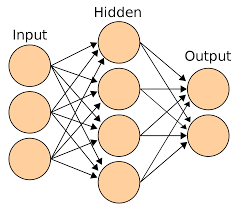
\includegraphics[scale=0.5]{figures/1174003/chapter6/1,2.png}
\caption{Ilustrasi Konsep dasar neural network}
\label{contoh}
\end{figure}


\item Jelaskan konsep pembobotan  dalam neural network. dilengkapidengan ilustrasi gambar. \par
pembobotan dalam neural network yaitu digunakan untuk membedakan objek inputan atau 
variabel inputan untuk AI. Dimana data inputan yang masuk adalah 2 data "nanas" dan "mangga" 
yang diolah dengan proses membandingkan data dan diolah melalui pembobotan sehingga menampilkan hasil output.

\begin{figure}[ht]
\centering
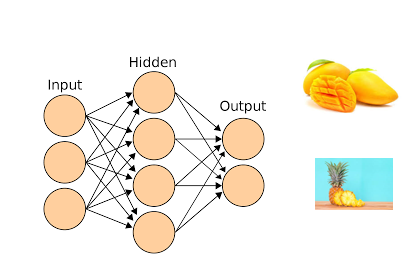
\includegraphics[scale=0.5]{figures/1174003/chapter6/1,3.PNG}
\caption{Ilustrasi Konsep pembobotan pada neural network}
\label{contoh}
\end{figure}

\item Jelaskan konsep aktifitas dalam neural network. dilengkapi dengan ilustrasi gambar.\par
Dalam Neural Network cara aktifitas dilakukan terhadap input pada neural network inputan tersebut dimasukan kepada 
fungsi pada mesin sehingga di hasilkanlah output yang sesuai dengan fungsi tersebut.

\begin{figure}[ht]
\centering
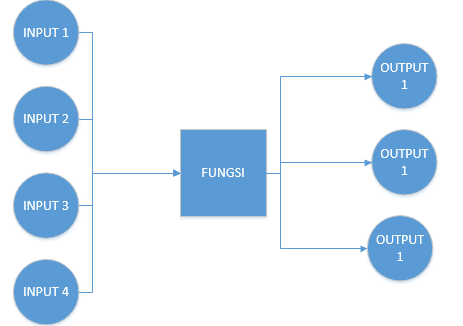
\includegraphics[scale=0.5]{figures/1174003/chapter6/1,4.PNG}
\caption{Gambar yang dibaca hasil plotnya}
\label{contoh}
\end{figure}

\item Jelaskan cara membaca hasil plot dari MFCC dilengkapi dengan ilustrasi gambar. \par
cara membaca hasil ploting dari MFCC yaitu tentukan terlebih dahulu batas minimal Hz dari 
gelombang suara dan batas maksimal dari suara tersebut. kemudian warna yang paling pekat merupakan hasil 
dari pengolahan data tersebut misalkan muncul warna orange pekat di bagian bawah dan orange muda di bagian atas
yang berarti suara tersebut kuat bagian basnya dan biasanya juga antara warna yang pekat tersebut ada jarak.

\begin{figure}[ht]
\centering
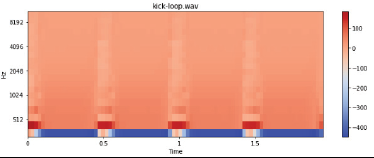
\includegraphics[scale=0.5]{figures/1174003/chapter6/1,5.PNG}
\caption{Ilustrasi Cara Membaca Hasil Plot}
\label{contoh}
\end{figure}

\item Jelaskan apa itu one-hot encoding, dilengkapi dengan ilustrasi kode atau gambar.\par
one-hot encoding merupakan pemberian nilai pada suatu variabel jika nilai itu positif 
maka nilainya satu dan jika negatif maka nilainya nol.

\begin{figure}[ht]
\centering
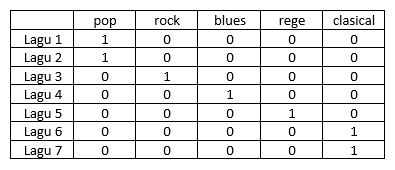
\includegraphics[scale=0.5]{figures/1174003/chapter6/1,6.PNG}
\caption{Ilustrasi Konsep one-hot encoding}
\label{contoh}
\end{figure}

\item Jelaskan apa dari np.unique dan to\_categorical dalam kode program, dilengkapi dengan ilustrasi atau gambar.\par
fungsi dari NP.UNIQUE dalah untuk membuat data elemen menjadi nilai yang bersifat unik dalam artian (Array). 
Sedangkan perintah to\_categorial adalah untuk membuat data integer yang terdeteksi untuk diubah menjadi data matrix biner. 
    
\begin{figure}[ht]
\centering
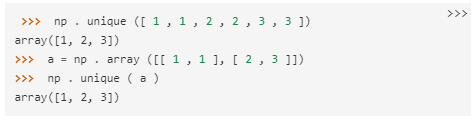
\includegraphics[scale=0.5]{figures/1174003/chapter6/1,7,1.PNG}
\caption{Ilustrasi np.unique}
\label{contoh}
\end{figure}

\begin{figure}[ht]
\centering
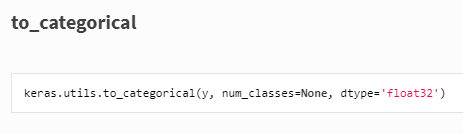
\includegraphics[scale=0.5]{figures/1174003/chapter6/1,7,2.PNG}
\caption{Ilustrasi to\_categorical}
\label{contoh}
\end{figure}


\item Jelaskan apa fungsi dari Sequential dalam kode program, dilengkapi dengan ilustrasi atau gambar. \par
fungsi dari Sequential dari code program adalah untuk membagi data - data agar dapat dianalisis oleh sistem lebih mudah, 
misalkan dari data 100 dibagi prosesnya menjadi 4 yaitu 25.
\begin{figure}[ht]
\centering
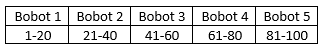
\includegraphics[scale=0.5]{figures/1174003/chapter6/1,8.PNG}
\caption{Ilustrasi Konsep pembobotan pada neural network}
\label{contoh}
\end{figure}

\end{enumerate}


\subsection{Praktikum}
\begin{enumerate}
\item Jelaskan isi dari data GTZAN Genre Collection dan data dari freesound. Buat kode program program untuk meload data tersebut untuk digunakan pada MFCC. Jelaskan arti dari perbaris kode yang dibuat (harus beda dengan teman satukelas).\par
\subitem Isi data data merupakan datasets lagu atau suara yang tersiri dari 10 gendre yang di simpan kedalam 10 folder yaitu folder blues, classical, country, disco, hiphop, jazz, metal, pop, reggae, dan rock ke sepuluh folder tersebut masing-masing  berisi 100 data suara sedangkan data freesound merupakan contoh data suara yang akan di gunakan untuk menguji hasil pengolahan data tersebut dengan menggunakan metode mfcc. apakah suara dari freesound termasuk kategori jazz pop atau sebagainya ?.

\lstinputlisting{src/1174003/chapter6/2,1.py}

\subitem dapat dilihat pada kode diatas pada baris kesatu dilakukan import librosa tang digunakan untuk fungsi mfcc pada suara.
pada baris kedua dilakukan import librosa featuse dan pada baris ke tiga dilakukan librosa display selanjutnya pada baris ke empat dilakukan import glob kemudian insert numpy untuk pengolahan data menjadi vektor setelah itu dilakukan import matplotlib untuk melakukan ploting setelah itu dilakukan import librari keras.\par

\subitem Selanjutnya yaitu membuat fungsi mfcc dengan nama display\_mfcc yang didalamnya terdapat variabel y yang berisi method librosa load kemudian variabel mfcc yang berisi method librosa featurea mfcc. Setelah itu membuat flot figure dengan ukuran 10 banding 4 kemudian di isi oleh data librosa display dengan variabel x nya yaitu waktu dan y yaitu mel atau Hz kemudian melakukan plot warna setelah itu melakukan plot judul dan terakhir flot di tampilkan. 

\item Jelaskan perbaris kode program dengan kata-kata dan di lengkapi ilustrasi gambar fungsi dari display\_mfcc().\par

\lstinputlisting{src/1174003/chapter6/2,2.py}

\subitem pada baris ke dua program diatas digunakan untuk mendisplay tampilan glombang suara dari file 266093\_\_stereo-surgeon\_\_kick-loop-5.wav menggunakan metode mfcc dengan menggunakan fungsi display\_mfcc yang telah tadi di buat pada nomer dua begitu juga pada baris ke 4 6 8 sampai ke 22 secara teksis sama menggunakan fungsi display\_mfcc hanyasaja beda peyimpanan data yang akan di tampilkan atau di eksekusi. untuk contoh hasilnya dapat dilihat pada gambar \ref{c122} berikut:
\begin{figure}[ht]
\centering
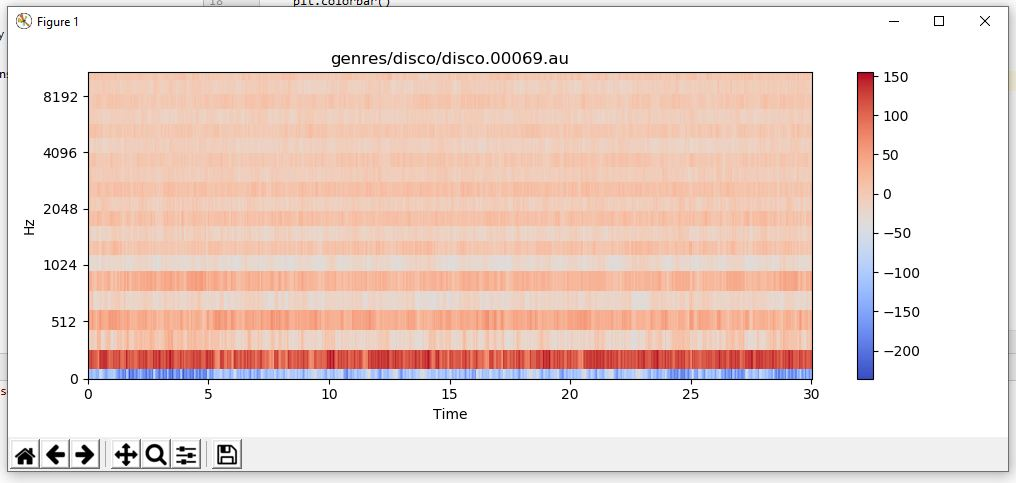
\includegraphics[scale=0.5]{figures/1174003/chapter6/2,2.JPG}
\caption{Ilustrasi gambar fungsi dari display\_mfcc() }
\label{contoh}
\end{figure}

Gambar tersebut merupakan hasil dari mfcc dari salah satu gender lagu pop yang ada pada datasets yang 1000 atau terdapat dalam sepuluh folder tadi.

\item Jelaskan perbaris dengan kata-kata dan dilengkapi dengan ilustrasi gambar fungsi dari extract\_features\_song jelaskan kenapa data yangdiambil merupakan data 25.000 baris pertama ? 

\lstinputlisting{src/1174003/chapter6/2,3.py}

\subitem pada baris ke tiga di definisikan nama extract\_features\_song yang nantinya akan di gunakan pada fungsi yang lainya kemudian dibuat variabel y dengan method librosa load setelah itu dibuat variabel baru mfcc dengan isi librosa features mfcc dengan isi variabel y tadi kemudian dibuat variabel mfcc dengan isian np.max dan variabel mfcc tadi terakhir di buat array dari data tersebut merupakan data 25000 data pertama. kenapa data 25000 pertama yang digunakan dikarenakan data tersebut digunakan sebagai data testing semakin besar data testing yang di gunakan maka semakin akurat hasil AI. tapi sebenarnya data tersebut relatif bisa lebih besar atau lebih kecil tergantung pada komputer masing masing.

\item Jelaskan Perbaris kode program dengan kata-kata dan di lengkapi ilustrasi gambar fungsi dari generate features and labels.

\lstinputlisting{src/1174003/chapter6/2,4.py}

\subitem pada baris ke tiga merupakan pendefinisian nama fungsi yaitu generate features and labels kemudian membuat variabel baru dengan array kosing yaitu all\_features dan all\_labels kemudian mendefinisikan isian label untuk gendre dengan cara membuat variabel genres kemudian di isi dengan 10 gendre yang tadi setelah itu dilakukan fungsi if else dengan code for dan in setelah itu akan di buat encoding untuk data tiap tiap label contoh untuk blues 1000000000 dan untuk clasical 0100000000.

\item Jelaskan dengan kata dan praktek kenapa penggunaan fungsi generate features and labels sangat lama saat meload dataset gendre tunjukan keluarannya dari komputer sendiri dan artikan maksud dari luaran tersebut.\par

halnini menjadi lama dikarenakan mesin membaca satupersatu file yang ada pada folder dan dalam foldertersebut terdapat 100 file sehingga wajar menjadi lama ditambah lagi mengolah data yang tadinya suara menjadi bentuk vektor. berikut merupakan codenya.
\lstinputlisting{src/1174003/chapter6/2,5.py}
\begin{figure}[ht]
\centering
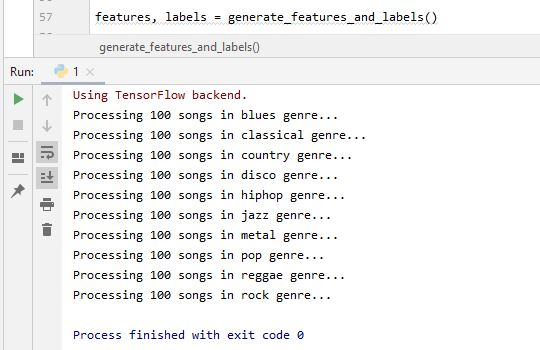
\includegraphics[scale=0.5]{figures/1174003/chapter6/2,5.JPG}
\caption{Hasil dari fungsi generate features and labels}
\label{contoh}
\end{figure}


\item jelaskan kenapa harus dilakukan pemisahan data training dan data testing sebesar 80 persen praktekan dengan kode dan tunjukan keluarannya dari komputer sendiri dan artikan maksud dari luaran tersebut. 
untuk code nya adalah sebagai berikut  yang merupakan code untuk membagi data sebanyak 80 persen untuk data training maka data musik tadi yang total jumlahnya 1000 akan di bagi dua untuk data training sebanyak 800  dan 200 untuk data testing.
\lstinputlisting{src/1174003/chapter6/2,6.py}


\item praktekan dan jelaskan masing masing parameter dari fungsi Sequential().  tunjukan keluarannya dari komputer sendiri dan artikan maksud dari luaran tersebut.\par
\subitem fungsi sequential digunakan untuk mengolah data inputan sesuai dengan fungsi yang ada pada fungsi sequential pada fungsi sequential kali ini menggunakan dua fungsi sequential mengkompile data dari 100 neuron atau dari 1 folder file dengan menggunakan fungsi relu dan softmax untuk menghasilkan outputan yang sesuai dengan keriteria.
\lstinputlisting{src/1174003/chapter6/2,7.py}


\item praktekan dan jelaskan masing masing parameter dari fungsi compile().  tunjukan keluarannya dari komputer sendiri dan artikan maksud dari luaran tersebut. \par
\subitem yaitu fungsi kompile yang digunakan untuk mengetahui parameter yang digunakan dari data yang telah diolah untuk caranya dapat menggunakan codingan sebagai berikut, pada gambar tersebut memunculkan parameternya berapasaja dan total parameter yang digunakan.
\lstinputlisting{src/1174003/chapter6/2,8.py}
\begin{figure}[ht]
\centering
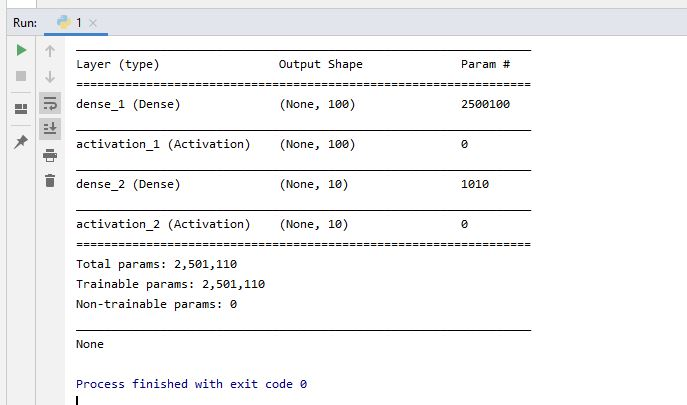
\includegraphics[scale=0.5]{figures/1174003/chapter6/2,8.JPG}
\caption{Hasil fungsi compile}
\label{contoh}
\end{figure}

\item praktekan dan jelaskan masing masing parameter dari fungsi fit().  tunjukan keluarannya dari komputer sendiri dan artikan maksud dari luaran tersebut.\par
\subitem pada fungsi ini dilakukan pengolahan data dari 10 label tadi atau 10 file data sets tadi kemudian di hitung tingkat akurasi masing masing dan tingkat kegagalan atau loss data darisetiap file tersebut caranya dengan melakukan codingan berikut. pada gambar tersebut menunjukan 10 pengolahan data untuk menentukan nilai akurasi dan loss dari data tersebut dan selanjutnya dilakukan fingsi evaluasi.
\lstinputlisting{src/1174003/chapter6/2,9.py}
\begin{figure}[ht]
\centering
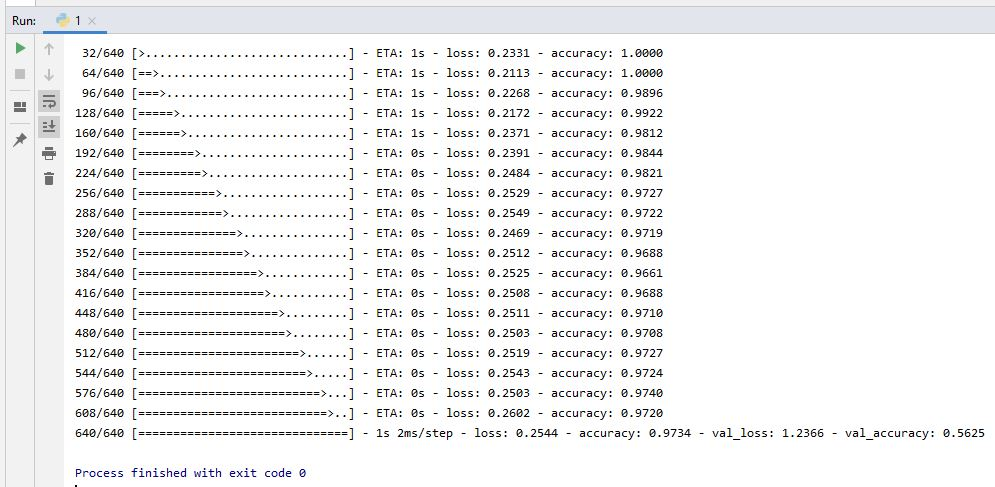
\includegraphics[scale=0.5]{figures/1174003/chapter6/2,9.JPG}
\caption{Hasil fungsi fit}
\label{contoh}
\end{figure}

\item praktekan dan jelaskan masing masing parameter dari fungsi evaluate().  tunjukan keluarannya dari komputer sendiri dan artikan maksud dari luaran tersebut.\par
\subitem pada fungsi ini dilakukan evaluasi terhadap datayang telah di runing sebelummnya untuk lebih jelasnya dapat di lihat codingan tersebut  pada codingan tersebut dilakukan evaluasi pada tingkat kegagalan dan akurasi kebenaran maka hasilnya munculkan hasil evaluasi dari 10 proses dari setiap gendre yaitu akurasi sebesar 51 persen dan loss data sebesar 1.4105 data.
\lstinputlisting{src/1174003/chapter6/2,10.py}
\begin{figure}[ht]
\centering
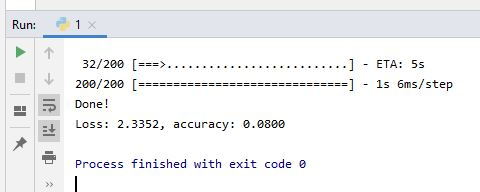
\includegraphics[scale=0.5]{figures/1174003/chapter6/2,10.JPG}
\caption{Hasil fungsi evaluasi}
\label{contoh}
\end{figure}

\item praktekan dan jelaskan masing masing parameter dari fungsi predic  tunjukan keluarannya dari komputer sendiri dan artikan maksud dari luaran tersebut. \par 
\subitem fungsi predic merupakan fungsi untuk membandingkan tingkat akurasi pada setiap label yang sepuluh tadi maka data akan di sandingkan ke masing masing tingkat akurasinya, yang akurasinya paling tinggi maka itulah jawaban untuk setiap inputan yang dilakukan. 
\lstinputlisting{src/1174003/chapter6/2,11.py}
\begin{figure}[ht]
\centering
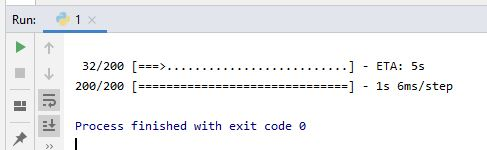
\includegraphics[scale=0.5]{figures/1174003/chapter6/2,11.JPG}
\caption{Hasil fungsi prediksi}
\label{contoh}
\end{figure}

\end{enumerate}



%\section{Evietania - 1174051}
\subsection{Teori}

\begin{enumerate}
\item Mengapa Kata-Kata Harus Di Lakukan Vektorisasi Dan Ilustrasi Gambar.
\begin{itemize}
\item Penjelasan:

Karenakan mesin hanya mampu membaca data dengan bentuk angka.Berdasarkan hal tersebut maka tentunya diperlukan vektorisasi kata atau bisa disebut dengan mengubah kata menjadi bentuk vektor agar mesin seolah-olah paham apa yang kita maksudkan dan dapat memproses aktifitas/perintah dengan benar. Selain alasan diatas, kata harus di vektorisasiuntuk mengetahui presentase kata yang sering muncul dalam setiap kalimatnya, yang berguna untuk menetukan kata kunci.

\item Ilustrasi Gambar

\begin{figure}[H]
\centering
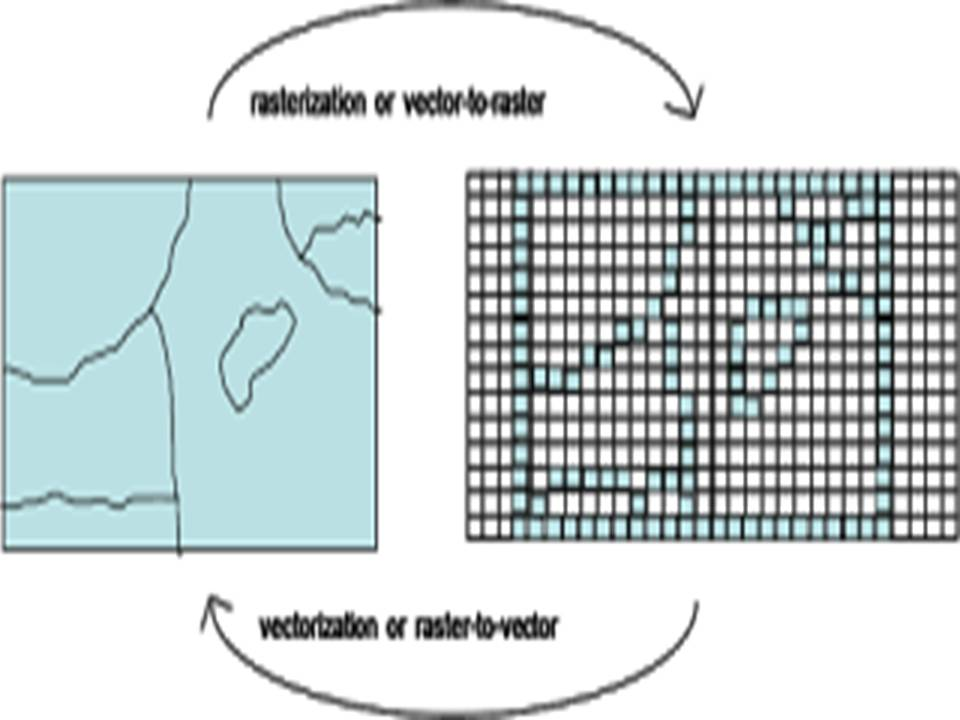
\includegraphics[scale=0.3]{figures/1174051/5/5.jpg}
\caption{Vektorisasi}
\label{Vektorisasi}
\end{figure}

\end{itemize}

\item Mengapa Dimensi Dari Vektor Dataset Google Bisa Mencapai 300 Dan Ilustrasi Gambar.
\begin{itemize}
\item Penjelasan:

Karena pada masing-masing objek yang terdapat pada dataset akan memiliki identitasnya tersendiri. Apabila dicontohkan dengan penjelasan yang lebih rinci maka dilakukan perumpamaan sederhana. Misalnya untuk sebuah dataset google yang memiliki 3 buah objek yaitu berat, lebar, dan tinggi.  Kemudian dari masing-masing objek tersebut dilakukan perbandingan antara berat dan lebar beserta berat dan tinggi. Hasil yang didapatkan akan memiliki presentasi yang berbeda sehingga dapat diartikan bahwa mesin dapat membedakan objek yang hampir serupa namun tak sama.

\item Ilustrasi Gambar

\begin{figure}[H]
\centering
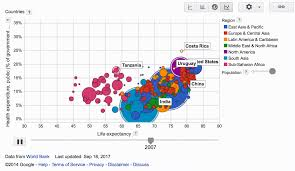
\includegraphics[scale=0.8]{figures/1174051/5/7.jpg}
\caption{Dimensi Vektor Dataset}
\label{Dimensi Vektor Dataset}
\end{figure}

\end{itemize}

\item Konsep Vektorisasi Untuk Kata Dan Ilustrasi Gambar.
\begin{itemize}
\item  Penjelasan:

Konsep untuk vektorisasi kata sebenarnya sama dengan ketika dilakukan input suatu kata pada mesin pencarian. Kemudian untuk hasilnya akan mengeluarkan ( berupa ) referensi mengenai kata tersebut. Jadi data kata tersebut didapatkan dari hasil pengolahan pada kalimat-kalimat sebelumnya yang telah diolah. Contoh sederhananya pada kalimat berikut ( Please click the alarm icon for more notifications about my channel ), pada kalimat tersebut terdapat konteks yakni channel, kata tersebut akan dijadikan data latih untuk mesin yang akan dipelajari dan diproses. Jadi ketika kita inputkan kta channel, maka mesin akan menampilkan keterkaitannya dengan kata tersebut sehingga akan lebih efisien dan lebih mudah.

\item Ilustrasi Gambar

\begin{figure}[H]
\centering
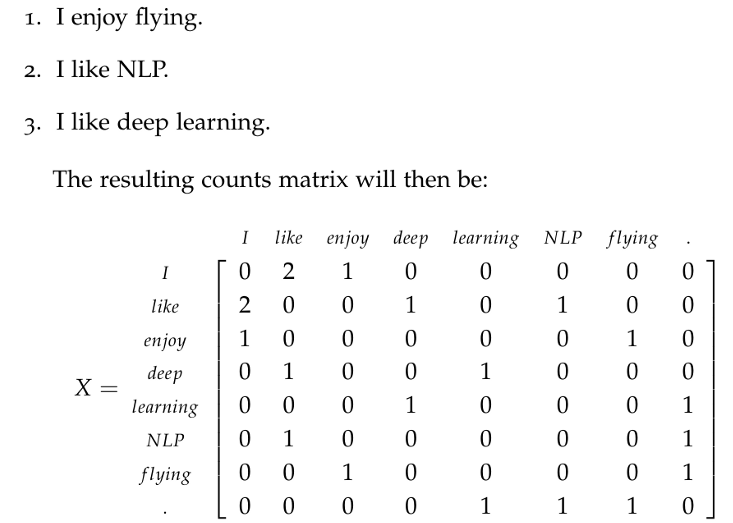
\includegraphics[scale=0.5]{figures/1174051/5/4.png}
\caption{Vektorisasi Untuk Kata}
\label{Vektorisasi Untuk Kata}
\end{figure}

\end{itemize}

\item Konsep Vektorisasi Untuk Dokumen Dan Ilustrasi Gambar.
\begin{itemize}
\item  Penjelasan:

Untuk vektorisasi dokumen sebenarnya terbilang sama dengan konsep vektorisasi kata, yang membedakan hanya pada proses awalnya ( pada eksekusi awal ). Untuk vektorisasi dokumen ini, mesin akan membaca semua kalimat yang terdapat pada dokumen tersebut, kemudian kalimat yang terdapat pada dokumen tersebut akan di pecah menjadi kata-kata. Seperti itulah konsep vektorisasi dokumen.

\item Ilustrasi Gambar

\begin{figure}[H]
\centering
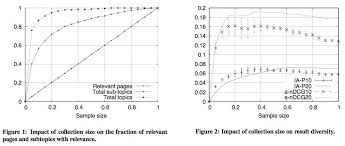
\includegraphics[scale=0.8]{figures/1174051/5/6.jpg}
\caption{Vektorisasi Untuk Dokumen}
\label{Vektorisasi Untuk Dokumen}
\end{figure}

\end{itemize}

\item Pengertian Mean Dan Standar Devisiasi Beserta Ilustrasi Gambar.
\begin{itemize}
\item  Pengertian Mean:

Mean adalah nilai rata-rata dari beberapa buah data. Nilai mean dapat ditentukan dengan membagi jumlah data dengan banyaknya data. Mean (rata-rata) merupakan suatu ukuran pemusatan data. Mean suatu data juga merupakan statistik karena mampu menggambarkan bahwa data tersebut berada pada kisaran mean data tersebut. Mean tidak dapat digunakan sebagai ukuran pemusatan untuk jenis data nominal dan ordinal.

\item  Pengertian Standar Devisiasi:

Standar Deviasi dan Varians Salah satu teknik statistik yg digunakan untuk menjelaskan homogenitas kelompok. Varians merupakan jumlah kuadrat semua deviasi nilai-nilai individual thd rata-rata kelompok. Sedangkan akar dari varians disebut dengan standar deviasi atau simpangan baku. Standar Deviasi dan Varians Simpangan baku merupakan variasi sebaran data. Semakin kecil nilai sebarannya berarti variasi nilai data makin sama Jika sebarannya bernilai 0, maka nilai semua datanya adalah sama. Semakin besar nilai sebarannya berarti data semakin bervariasi.

\item Ilustrasi Gambar

\begin{figure}[H]
\centering
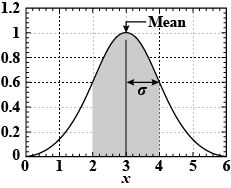
\includegraphics[scale=0.7]{figures/1174051/5/2.png}
\caption{Mean}
\label{Mean}
\end{figure}

\begin{figure}[H]
\centering
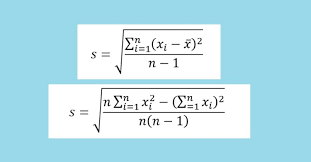
\includegraphics[scale=0.7]{figures/1174051/5/3.png}
\caption{Standar Devisiasi}
\label{Standar Devisiasi}
\end{figure}

\end{itemize}

\item Penjelasan Skip-gram Dan Ilustrasi Gambar
\begin{itemize}
\item  Penjelasan:

Skip-Gram adalah kebalikannya, yaitu mencoba memprediksi vektor kata-kata yang ada di konteks diberikan vektor kata tertentu. Skip-Gram membuat sepasang kata target dan konteks sebagai sebuah instance sehingga Skip-Gram cenderung lebih baik ketika ukuran corpus sangat besar. 

\item Ilustrasi Gambar

\begin{figure}[H]
\centering
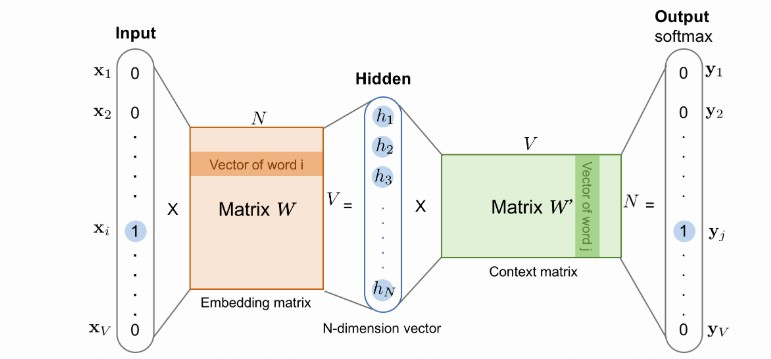
\includegraphics[scale=0.5]{figures/1174051/5/1.jpg}
\caption{Skip Gram}
\label{Skip Gram}
\end{figure}
\par
\par
\end{itemize}
\par
\par
\end{enumerate}

\subsection{Praktek}
\begin{enumerate}
\item Percobaan Google Dataset ( Perbandingan Dan Similarity ) Untuk Beberapa Data Berikut :
\begin{enumerate}
\item Love

Penjelasan: Pada hasil gambar 'love' dapat dilihat bahwa nilai pada vektor baris pertamanya adalah 0.10302734. Jika dibandingkan dengan gambar 'faith' dapat dikatakan bahwa kedua gambar tersebut tidak dapat dimasukkan pada kategori yang sama.

\begin{figure}[H]
\centering
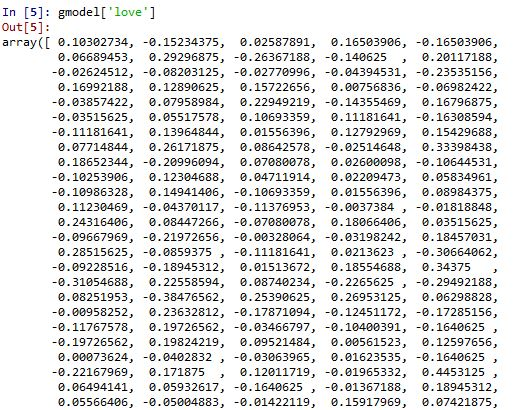
\includegraphics[scale=0.7]{figures/1174051/5/12love.jpg}
\caption{Google Dataset}
\label{Google Dataset}
\end{figure}

\item Faith

Penjelasan: Pada hasil gambar 'faith' dapat dilihat bahwa nilai pada vektor baris pertamanya adalah 0.26367188. Jika dibandingkan dengan gambar 'fall' dapat dikatakan bahwa kedua gambar tersebut tidak dapat dimasukkan pada kategori yang sama.

\begin{figure}[H]
\centering
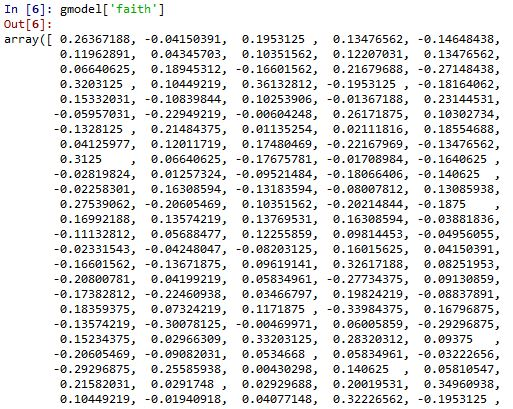
\includegraphics[scale=0.7]{figures/1174051/5/13faith.jpg}
\caption{Google Dataset}
\label{Google Dataset}
\end{figure}

\item Fall

Penjelasan: Pada hasil gambar 'fall' dapat dilihat bahwa nilai pada vektor baris pertamanya adalah -0.04272461. Jika dibandingkan dengan gambar 'sick' dapat dikatakan bahwa kedua gambar tersebut tidak dapat dimasukkan pada kategori yang sama.

\begin{figure}[H]
\centering
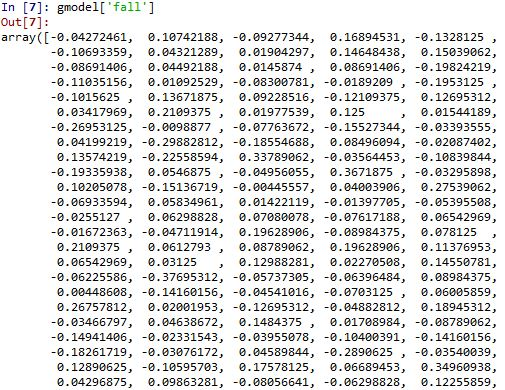
\includegraphics[scale=0.7]{figures/1174051/5/14fall.jpg}
\caption{Google Dataset}
\label{Google Dataset}
\end{figure}

\item Sick

Penjelasan: Pada hasil gambar 'sick' dapat dilihat bahwa nilai pada vektor baris pertamanya adalah 1.82617188e-01. Jika dibandingkan dengan gambar 'clear' dapat dikatakan bahwa kedua gambar tersebut tidak dapat dimasukkan pada kategori yang sama.

\begin{figure}[H]
\centering
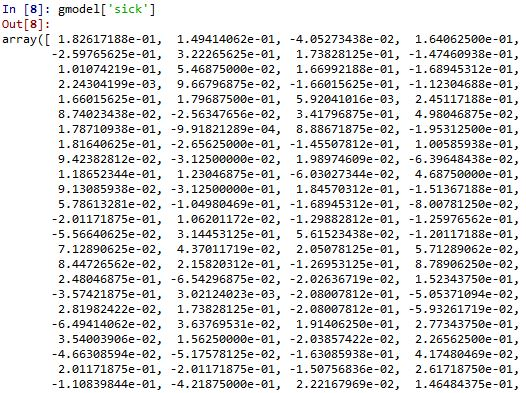
\includegraphics[scale=0.7]{figures/1174051/5/15sick.jpg}
\caption{Google Dataset}
\label{Google Dataset}
\end{figure}

\item Clear

Penjelasan: Pada hasil gambar 'clear' dapat dilihat bahwa nilai pada vektor baris pertamanya adalah -2.44140625e-04. Jika dibandingkan dengan gambar 'shine' dapat dikatakan bahwa kedua gambar tersebut tidak dapat dimasukkan pada kategori yang sama.

\begin{figure}[H]
\centering
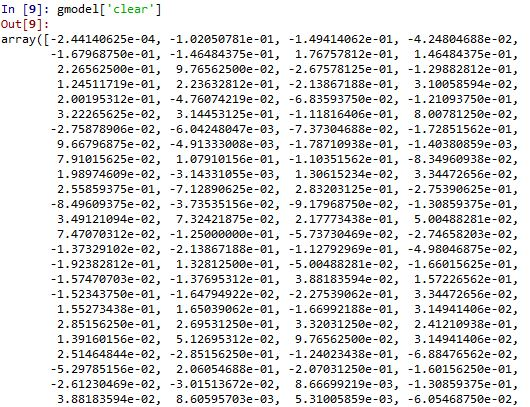
\includegraphics[scale=0.7]{figures/1174051/5/16clear.jpg}
\caption{Google Dataset}
\label{Google Dataset}
\end{figure}

\item Shine

Penjelasan: Pada hasil gambar 'shine' dapat dilihat bahwa nilai pada vektor baris pertamanya adalah -0.12402344. Jika dibandingkan dengan gambar 'bag' dapat dikatakan bahwa kedua gambar tersebut tidak dapat dimasukkan pada kategori yang sama.

\begin{figure}[H]
\centering
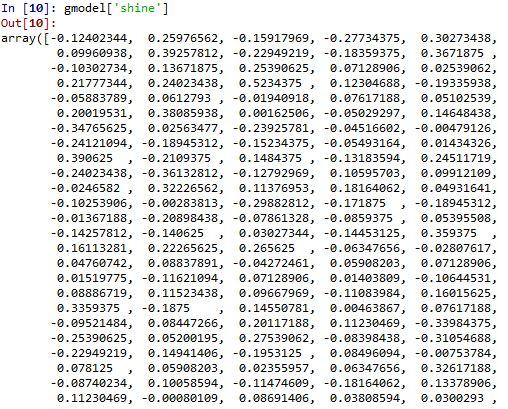
\includegraphics[scale=0.7]{figures/1174051/5/17shine.jpg}
\caption{Google Dataset}
\label{Google Dataset}
\end{figure}

\item Bag

Penjelasan: Pada hasil gambar 'bag' dapat dilihat bahwa nilai pada vektor baris pertamanya adalah -0.03515625. Jika dibandingkan dengan gambar 'car' dapat dikatakan bahwa kedua gambar tersebut tidak dapat dimasukkan pada kategori yang sama.

\begin{figure}[H]
\centering
\includegraphics[scale=0.7]{figures/1174051/5/18bag.jpg}
\caption{Google Dataset}
\label{Google Dataset}
\end{figure}

\item Car

Penjelasan: Pada hasil gambar 'car' dapat dilihat bahwa nilai pada vektor baris pertamanya adalah 0.13085938. Jika dibandingkan dengan gambar 'wash' dapat dikatakan bahwa kedua gambar tersebut tidak dapat dimasukkan pada kategori yang sama.

\begin{figure}[H]
\centering
\includegraphics[scale=0.7]{figures/1174051/5/19car.jpg}
\caption{Google Dataset}
\label{Google Dataset}
\end{figure}

\item Wash

Penjelasan: Pada hasil gambar 'wash' dapat dilihat bahwa nilai pada vektor baris pertamanya adalah 9.46044922e-03. Jika dibandingkan dengan gambar 'motor' dapat dikatakan bahwa kedua gambar tersebut tidak dapat dimasukkan pada kategori yang sama.

\begin{figure}[H]
\centering
\includegraphics[scale=0.7]{figures/1174051/5/20wash.jpg}
\caption{Google Dataset}
\label{Google Dataset}
\end{figure}

\item Motor

Penjelasan: Pada hasil gambar 'motor' dapat dilihat bahwa nilai pada vektor baris pertamanya adalah 5.73730469e-02. Jika dibandingkan dengan gambar 'cycle' dapat dikatakan bahwa kedua gambar tersebut tidak dapat dimasukkan pada kategori yang sama.

\begin{figure}[H]
\centering
\includegraphics[scale=0.7]{figures/1174051/5/21motor.jpg}
\caption{Google Dataset}
\label{Google Dataset}
\end{figure}

\item Cycle

Penjelasan: Pada hasil gambar 'cycle' dapat dilihat bahwa nilai pada vektor baris pertamanya adalah 0.04541016. Jika dibandingkan dengan gambar 'love' dapat dikatakan bahwa kedua gambar tersebut tidak dapat dimasukkan pada kategori yang sama.

\begin{figure}[H]
\centering
\includegraphics[scale=0.7]{figures/1174051/5/22cycle.jpg}
\caption{Google Dataset}
\label{Google Dataset}
\end{figure}

\item Similarity

Penjelasan: Pada hasil gambar 'car' dapat dilihat bahwa nilai pada vektor baris pertamanya adalah 0.13085938. Jika dibandingkan dengan gambar 'love', 'sick', 'clear', 'motor', 'wash' dapat dikatakan bahwa semua gambar tersebut yang paling mendekati adalah 'sick'.

\begin{figure}[H]
\centering
\includegraphics[scale=0.7]{figures/1174051/5/23.jpg}
\caption{Google Dataset}
\label{Google Dataset}
\end{figure}

\end{enumerate}

\item Penjelasan Dan Ilustrasi ExtractWords Dan PermuteSentences
\begin{itemize}

\begin{figure}[H]
\centering
\includegraphics[scale=0.7]{figures/1174051/5/32.jpg}
\caption{Extract Word dan PermuteSentence}
\label{Extract Word dan PermuteSentence}
\end{figure}

\item ExtractWords

Penjelasan:  Pada kalimat 'This isn't really a sentence' yang  akan dipisahkan perkata. Dimana library re dan library string di import terlebih dahulu. Lalu variable out mendefinisikan X untuk mengembalikan string pada objek line yang telah di split. Kemudian, X dikembalikan berdasarkan jumlah kata.

\begin{figure}[H]
\centering
\includegraphics[scale=0.7]{figures/1174051/5/29.jpeg}
\caption{ExtractWord}
\label{ExtractWord}
\end{figure}

\item PermuteSentences

Penjelasan: Digunakan untuk melakukan pengocokan atau acak pada text yang diiginkan.

\begin{figure}[H]
\centering
\includegraphics[scale=0.7]{figures/1174051/5/31.jpg}
\caption{PermuteSentences}
\label{PermuteSentences}
\end{figure}

\end{itemize}

\item Library Gensim TaggedDocument Dan Doc2Vac
\begin{itemize}
\item Contoh atau Ilustrasi Gambar:

\begin{figure}[H]
\centering
\includegraphics[scale=0.7]{figures/1174051/5/40.jpg}
\caption{Tagged Document dan Doc2Vec}
\label{Tagged Document dan Doc2Vec}
\end{figure}

Penjelasan:

Import library gensim dan meng-import modul Tagged Document dan Doc2Vac.Tagged Document adalah dokumen yang 'memisahkan informasi dan struktur dari presentasi' dengan menggunakan tag. Fungsi Doc2Vec berisi alpha dan min alpha parameter, tetapi itu berarti bahwa tingkat pembelajaran meluruh selama satu periode dari alpha untuk min alpha.

\end{itemize}

\item Menambahkan Data Training (Melatih Modul Doc2Vec)
\begin{itemize}
\item Contoh atau Ilustrasi Gambar:

\begin{figure}[H]
\centering
\includegraphics[scale=0.7]{figures/1174051/5/42.jpg}
\caption{Model 1}
\label{Model 1}
\end{figure}

\begin{figure}[H]
\centering
\includegraphics[scale=0.7]{figures/1174051/5/43.jpg}
\caption{Model 2}
\label{Model 2}
\end{figure}

\begin{figure}[H]
\centering
\includegraphics[scale=0.7]{figures/1174051/5/44.jpg}
\caption{Model 3}
\label{Model 3}
\end{figure}

Penjelasan:

Membaca direktori name dari data yang ada di dalam kurung, terdapat ada 3 data.

\end{itemize}

\item Pengocokan Dan Pembersihan Data.
\begin{itemize}
\item Contoh atau Ilustrasi Gambar: 

\begin{figure}[H]
\centering
\includegraphics[scale=0.7]{figures/1174051/5/60.jpg}
\caption{Pengocokan dan Pembersihan Data}
\label{Pengocokan dan Pembersihan Data}
\end{figure}

\begin{figure}[H]
\centering
\includegraphics[scale=0.7]{figures/1174051/5/61.jpg}
\caption{Pengocokan dan Pembersihan Data}
\label{Pengocokan dan Pembersihan Data}
\end{figure}

Penjelasan:

Mengimport Library Re. Kemudian membuat fungsi utuk menghapus tag html dan perkocokan. Dimana di dalam variabel ini ada kodingan untuk menghapus tag html yaitu petik satu, tanda baca dan spasi yang berurutan. Melakukan pengacakan model terhadap data unsupervised learning. Dan kemudian baru membuat modelnya setelah dilakukan pengacakan terhadap yang pertama tadi.

\end{itemize}

\item Mengapa Model Harus Di Save Dan Temporari Training Harus Dihapus
\begin{itemize}
\item Contoh atau Ilustrasi Gambar:

\begin{figure}[H]
\centering
\includegraphics[scale=0.7]{figures/1174051/5/49.jpg}
\caption{Model Disave dan Temporari Train Hapus}
\label{Model Disave dan Temporari Train Hapus}
\end{figure}

\begin{figure}[H]
\centering
\includegraphics[scale=0.7]{figures/1174051/5/50.jpg}
\caption{Model Disave dan Temporari Train Hapus}
\label{Model Disave dan Temporari Train Hapus}
\end{figure}

Penjelasan:

Untuk mencegah ram agar tidak lemot atau lambat. Sedangkan kenapa temporari training harus dihapus mengosongkan memori agar sedikit lega atau tidak lemot.

\end{itemize}

\item Infercode
\begin{itemize}
\item Contoh atau Ilustrasi Gambar:

\begin{figure}[H]
\centering
\includegraphics[scale=0.7]{figures/1174051/5/51.jpg}
\caption{Infercode}
\label{Infercode}
\end{figure}

Penjelasan:

Untuk menyimpulkan vektor yang berhubungan dengan vektor dokumen baru dan output tersebut merupakan sebuah array.

\end{itemize}

\item Cosinesimilarity
\begin{itemize}
\item Contoh atau Ilustrasi Gambar:

\begin{figure}[H]
\centering
\includegraphics[scale=0.7]{figures/1174051/5/52.jpg}
\caption{Cosinesimilarity}
\label{Cosinesimilarity}
\end{figure}

\begin{figure}[H]
\centering
\includegraphics[scale=0.7]{figures/1174051/5/53.jpg}
\caption{Cosinesimilarity}
\label{Cosinesimilarity}
\end{figure}

\begin{figure}[H]
\centering
\includegraphics[scale=0.7]{figures/1174051/5/54.jpg}
\caption{Cosinesimilarity}
\label{Cosinesimilarity}
\end{figure}

\begin{figure}[H]
\centering
\includegraphics[scale=0.7]{figures/1174051/5/55.jpg}
\caption{Cosinesimilarity}
\label{Cosinesimilarity}
\end{figure}

Penjelasan: 

Cosine Similarity dapat diimplementasikan untuk menghitung nilai kemiripan antar kalimat dan menjadi salah satu teknik untuk mengukur kemiripan  teks yang  popular. 

\end{itemize}

\item Praktek Score Dari Cross Validation
\begin{itemize}
\item Contoh atau Ilustrasi Gambar:

\begin{figure}[H]
\centering
\includegraphics[scale=0.7]{figures/1174051/5/56.jpg}
\caption{Score Cross Validation}
\label{Score Cross Validation}
\end{figure}

\begin{figure}[H]
\centering
\includegraphics[scale=0.7]{figures/1174051/5/57.jpg}
\caption{Score Cross Validation}
\label{Score Cross Validation}
\end{figure}

\begin{figure}[H]
\centering
\includegraphics[scale=0.7]{figures/1174051/5/58.jpg}
\caption{Score Cross Validation}
\label{Score Cross Validation}
\end{figure}

\begin{figure}[H]
\centering
\includegraphics[scale=0.7]{figures/1174051/5/59.jpg}
\caption{Score Cross Validation}
\label{Score Cross Validation}
\end{figure}

Penjelasan: 

Hasil dari praktek tersebut menunjukan untuk menghitung memprediksi dan mengetahui keakuratan dari suatu nilai.

\item PENANGANAN ERROR
\begin{itemize}
\item Contoh atau Ilustrasi Gambar:

\begin{figure}[H]
\centering
\includegraphics[scale=0.7]{figures/1174051/5/11Error.jpg}
\caption{Error}
\label{Error}
\end{figure}

Solusi:

Pastikan dataset berada dalam satu folder.

\end{itemize}
\end{itemize}
\end{enumerate}
%\section{1174003 - Dwi Septiani Tsaniyah}
\subsection{Soal Teori}
\begin{enumerate}

	\item Jelaskan kenapa file suara harus di lakukan MFCC. dilengkapi dengan ilustrasi atau gambar.
	\hfill\break
	Karena MFCC adalah koefisien yang mewakili audio. Ekstraksi fitur dalam proses ini ditandai dengan konversi data suara menjadi gambar spektrum gelombang. File audio dilakukan oleh MFCC sehingga objek suara dapat dikonversi menjadi matriks. Suara akan menjadi vektor yang akan diproses sebagai output. Selain mempermudah mesin dalam bahasa ini karena mesin tidak dapat membaca teks, maka MFCC perlu mengubah suara menjadi vektor. Untuk ilustrasi, lihat gambar berikut: 

	\begin{figure}[H]
	\centering
		\includegraphics[width=4cm]{figures/1174021/tugas6/materi/teori1.PNG}
		\caption{Teori 1}
	\end{figure}

	\item Jelaskan konsep dasar neural network.dilengkapi dengan ilustrasi atau gambar.
	\hfill\break
	Konsep sederhana dari neural network atau jaringan saraf sederhana dengan proses pembelajaran pada anak-anak dengan memetakan pola-pola baru yang diperoleh dari input untuk membuat pola-pola baru pada output. Contoh sederhana ini menganalogikan kinerja otak manusia. Jaringan saraf itu sendiri terdiri dari unit pemrosesan yang disebut neuron yang berisi fungsi adder dan aktivasi. Fungsi aktivasi itu sendiri untuk publikasi diberikan oleh neuron. Jaringan saraf yang mendukung pemikiran sistem atau aplikasi yang melibatkan otak manusia, baik untuk mendukung berbagai elemen sinyal yang diterima, memeriksa kesalahan, dan juga memproses secara paralel. Karakteristik neural network atau jaringan saraf dilihat dari pola hubungan antar neuron, metode penentuan bobot setiap koneksi, dan fungsi aktivasi mereka.. Untuk ilustrasi, lihat gambar berikut: 

	\begin{figure}[H]
	\centering
		\includegraphics[width=4cm]{figures/1174021/tugas6/materi/teori2.PNG}
		\caption{Teori 2}
	\end{figure}
	
	\item Jelaskan konsep pembobotan dalam neural network.dilengkapi dengan ilustrasi atau gambar.
	\hfill\break
	Pembobotan di dalam neural network juga akan menentukan penanda konektivitas. Dalam proses neural network mulai dari input yang diterima oleh neuron bersama dengan nilai bobot masing-masing input. Setelah memasuki neuron, nilai input akan ditambahkan oleh fungsi penerima. Hasil penambahan ini akan diproses oleh masing-masing fungsi neuron, hasil penambahan ini akan dibandingkan dengan nilai ambang tertentu. Jika nilai jumlah ini melebihi nilai ambang batas, aktivasi neuron akan dibatalkan, tetapi sebaliknya jika jumlah hasil di bawah nilai ambang batas, neuron akan diaktifkan. Setelah neuron aktif maka akan mengirimkan nilai output melalui bobot outputnya ke semua neuron yang terkait. Untuk ilustrasi, lihat gambar berikut: 

	\begin{figure}[H]
	\centering
		\includegraphics[width=4cm]{figures/1174021/tugas6/materi/teori3.PNG}
		\caption{Teori 3}
	\end{figure}

	\item Jelaskan konsep fungsi aktifasi dalam neural network. dilengkapi dengan ilustrasi atau gambar.
	\hfill\break
	Fungsi aktivasi dalam neural network ialah merupakan suatu operasi matematik yang dikenakan pada sinyal output. Fungsi ini digunakan untuk mengaktifkan atau menonaktifkan neuron. Fungsi aktivasi ini terbagi setidaknya menjadi 6, adapun sebagai berikut:
	\begin{itemize}
	\item Fungsi Undak Biner Hard Limit, fungsi ini biasanya digunakan oleh jaringan lapiran tunggal untuk mengkonversi nilai input dari suatu variabel yang bernilai kontinu ke suatu nilai output biner 0 atau 1.
	\item Fungsi Undak Biner Threshold, fungsi ini menggunakan nilai ambang sebagai batasnya.
	\item Fungsi Bipolar Symetric Hard Limit, fungsi ini memiliki output bernilai 1, 0 atau -1.
	\item Fungsi Bipolar dengan Threshold, fungsi ini mempunyai output yang bernilai 1, 0 atau -1 untuk batas nilai ambang tertentu.
	\item Fungsi Linear atau Identitas.
	\end{itemize}. 
	Namun, untuk ilustrasi lihat gambar berikut: 

	\begin{figure}[H]
	\centering
		\includegraphics[width=4cm]{figures/1174021/tugas6/materi/teori4.PNG}
		\caption{Teori 4}
	\end{figure}

	\item Jelaskan cara membaca hasil plot dari MFCC,dilengkapi dengan ilustrasi atau gambar
	\hfill\break
	Perhatikan gambar dibawah: Gambar menjelaskan bahwa pada waktu ke-5 kekuatan atau layak yang dikeluarkan pada nada ini paling keras pada 20 Hz, selain itu pada 40 -120 Hz daya atau nilai dikeluarkan pada musik yang telah diplot. Demikian juga, warna terseksi adalah kekuatan atau nilai tertinggi dibandingkan dengan warna canggih. Yang merah terdengar di bawah pendengaran manusia, sehingga tidak bisa didengar secara langsung.

	\begin{figure}[H]
	\centering
		\includegraphics[width=4cm]{figures/1174021/tugas6/materi/teori5.PNG}
		\caption{Teori 5}
	\end{figure}

	\item Jelaskan apa itu one-hot encoding,dilengkapi dengan ilustrasi kode dan atau gambar.
	\hfill\break
	Sederhananya, one-hot encoding ini adalah untuk mengubah hasil data vektorisasi menjadi angka biner 0 dan 1 dan membuat informasi tentang atribut yang diberi label. Untuk ilustrasi, lihat gambar berikut: 

	\begin{figure}[H]
	\centering
		\includegraphics[width=4cm]{figures/1174021/tugas6/materi/teori6_1.PNG}
		\includegraphics[width=4cm]{figures/1174021/tugas6/materi/teori6_2.PNG}
		\caption{Teori 6}
	\end{figure}

	\item Jelaskan apa fungsi dari np.unique dan to categorical dalam kode program,dilengkapi dengan ilustrasi atau gambar.
	\hfill\break
	Fungsi np.unique adalah untuk menemukan berbagai elemen atau array unik, dan dapat mengembalikan elemen unik dari array yang diurutkan. Sebagai ilustrasi, cukup bisa dilihat pada gambar di bawah ini. Gambar tersebut menjelaskan bahwa unik itu sendiri akan mengambil data yang berbeda dari variabel a dalam fungsi array.

	\begin{figure}[H]
	\centering
		\includegraphics[width=4cm]{figures/1174021/tugas6/materi/teori7_1.PNG}
		\caption{Teori 7}
	\end{figure}

	Fungsi dari to\_categorical ialah untuk mengubah suatu vektor yang berupa integer menjadi matrix dengan kelas biner. Untuk ilustrasinya bisa dilihat pada gambar \ref{cc71}
		\begin{figure}[H]
	\centering
		\includegraphics[width=4cm]{figures/1174021/tugas6/materi/teori7_2.PNG}
		\caption{Teori 7}
	\end{figure}

	\item Jelaskan apa fungsi dari Sequential dalam kode program,dilengkapi dengan ilustrasi atau gambar.
	\hfill\break
	Fungsi dari Sequential sebagai salah satu jenis model yang digunakan dalam perhitungan. Sequential ini membangun tumpukan linear yang berurutan. Untuk ilusrasi gambar sebagai betikut : 

	\begin{figure}[H]
	\centering
		\includegraphics[width=4cm]{figures/1174021/tugas6/materi/teori8.PNG}
		\caption{Teori 8}
	\end{figure}
\end{enumerate}

\subsection{Praktek Program}
\begin{enumerate}
	\item Soal 1
	\hfill\break
	\lstinputlisting[firstline=7, lastline=28]{src/1174021/tugas6/tugas6.py}
	Kode di atas menjelaskan isi data GTZAN. Ini adalah kumpulan data yang berisi 10 genre lagu dengan masing-masing genre memiliki 100 lagu yang akan kami lakukan proses MFCC dan juga freesound yang hanya berisi konten lagu, jika GTZAN memiliki beberapa genre jika freesound hanya untuk 1 lagu dan disini kita membuat fungsi untuk membaca file audio dan outputnya sebagai plot, hasilnya adalah sebagai berikut:
	\begin{figure}[H]
	\centering
		\includegraphics[width=4cm]{figures/1174021/tugas6/materi/hasil1.PNG}
		\caption{Hasil Soal 1.}
	\end{figure}

	\item Soal 2
	\hfill\break
	\lstinputlisting[firstline=29, lastline=50]{src/1174021/tugas6/tugas6.py}
	Kode di atas akan menampilkan hasil dari proses mfcc yang sudah dibuat fungsi pada soal 1, yaitu display mfcc() dan akan menampilkan plot dari pembacaan file audio. Berikut adalah hasil setelah saya lakukan running dan pembacaan file audio :
	\begin{figure}[H]
	\centering
		\includegraphics[width=4cm]{figures/1174021/tugas6/materi/hasil2_1.PNG}
		\includegraphics[width=4cm]{figures/1174021/tugas6/materi/hasil2_2.PNG}
		\includegraphics[width=4cm]{figures/1174021/tugas6/materi/hasil2_3.PNG}
		\includegraphics[width=4cm]{figures/1174021/tugas6/materi/hasil2_4.PNG}
		\includegraphics[width=4cm]{figures/1174021/tugas6/materi/hasil2_5.PNG}
		\includegraphics[width=4cm]{figures/1174021/tugas6/materi/hasil2_6.PNG}
		\includegraphics[width=4cm]{figures/1174021/tugas6/materi/hasil2_7.PNG}
		\includegraphics[width=4cm]{figures/1174021/tugas6/materi/hasil2_8.PNG}
		\includegraphics[width=4cm]{figures/1174021/tugas6/materi/hasil2_9.PNG}
		\includegraphics[width=4cm]{figures/1174021/tugas6/materi/hasil2_10.PNG}
		\includegraphics[width=4cm]{figures/1174021/tugas6/materi/hasil2_11.PNG}
		\caption{Hasil Soal 2.}
	\end{figure}

	\item Soal 3
	\hfill\break
	\lstinputlisting[firstline=51, lastline=61]{src/1174021/tugas6/tugas6.py}
	Baris pertama itu untuk membuat fungsi extract\_features\_song(f). Pada baris kedua itu akan me-load data inputan dengan menggunakan librosa. Lalu selanjutnya untuk membuat sebuah fitur untuk mfcc dari y atau parameter inputan. Lalu akan me-return menjadi array dan akan mengambil 25000 data saja dari hasil vektorisasi dalam 1 lagu. Hasilnya adalah sebagai berikut :
	\begin{figure}[H]
	\centering
		\includegraphics[width=4cm]{figures/1174021/tugas6/materi/hasil3.PNG}
		\caption{Hasil Soal 3.}
	\end{figure}

	\item Soal 4
	\hfill\break
	\lstinputlisting[firstline=63, lastline=82]{src/1174021/tugas6/tugas6.py}
	Kode di atas dapat digunakan untuk melakukan fungsi yang sebelumnya telah kita lakukan. Kemudian di bagian genre yang disesuaikan dengan dataset nama folder. Untuk baris berikutnya akan mengulang genre folder dengan ekstensi .au. Maka itu akan memanggil fungsi ekstrak lagu. Setiap file dalam folder itu akan diekstraksi menjadi vektor dan akan ditambahkan ke fitur. Dan fungsi yang ditambahkan adalah untuk menumpuk file yang telah di-vektor-kan. Hasil kode tidak menampilkan output. Hasilnya adalah sebagai berikut :
	\begin{figure}[H]
	\centering
		\includegraphics[width=4cm]{figures/1174021/tugas6/materi/hasil4.PNG}
		\caption{Hasil Soal 4.}
	\end{figure}

	\item Soal 5
	\hfill\break
	\lstinputlisting[firstline=84, lastline=89]{src/1174021/tugas6/tugas6.py}
	Kode diatas berfungsi untuk melakukan load variabel features dan labels. Mengapa memakan waktu yang lama ? Karena mesin akan melakukan vektorisasi terhadap semua file yang berada pada setiap foldernya, di sini terdapat 10 folder dengan masing-masing folder terdiri atas 100 buah lagu, setiap lagu tersebut akan dilakukan vektorisasi atau ekstraksi data menggunakan mfcc. Oleh karena itu, proses cukup memakan waktu. Hasilnya adalah sebagai berikut :
	\begin{figure}[H]
	\centering
		\includegraphics[width=4cm]{figures/1174021/tugas6/materi/hasil5_1.PNG}
		\includegraphics[width=4cm]{figures/1174021/tugas6/materi/hasil5_2.PNG}
		\includegraphics[width=4cm]{figures/1174021/tugas6/materi/hasil5_3.PNG}
		\caption{Hasil Soal 5.}
	\end{figure}

	\item Soal 6
	\hfill\break
	\lstinputlisting[firstline=90, lastline=109]{src/1174021/tugas6/tugas6.py}
	Kode diatas berfungsi untuk melakukan training split 80\%. Karena supaya mesin dapat terus belajar tentang data baru, jadi ketika prediksi dibuat tentang data yang terlatih itu bisa mendapatkan persentase yang cukup bagus. Hasilnya adalah sebagai berikut :
	\begin{figure}[H]
	\centering
		\includegraphics[width=4cm]{figures/1174021/tugas6/materi/hasil6_1.PNG}
		\includegraphics[width=4cm]{figures/1174021/tugas6/materi/hasil6_2.PNG}
		\includegraphics[width=4cm]{figures/1174021/tugas6/materi/hasil6_3.PNG}
		\includegraphics[width=4cm]{figures/1174021/tugas6/materi/hasil6_4.PNG}
		\includegraphics[width=4cm]{figures/1174021/tugas6/materi/hasil6_5.PNG}
		\includegraphics[width=4cm]{figures/1174021/tugas6/materi/hasil6_6.PNG}
		\includegraphics[width=4cm]{figures/1174021/tugas6/materi/hasil6_7.PNG}
		\includegraphics[width=4cm]{figures/1174021/tugas6/materi/hasil6_8.PNG}
		\caption{Hasil Soal 6.}
	\end{figure}

	\item Soal 7
	\hfill\break
	\lstinputlisting[firstline=111, lastline=117]{src/1174021/tugas6/tugas6.py}
	fungsi Sequential() ialah Sebuah model untuk menentukan izin pada setiap neuron, di sini adalah 100 dense yang merupakan 100 neuron pertama dari data pelatihan. Fungsi dari relay itu sendiri adalah untuk mengaktifkan neuron atau input yang memiliki nilai maksimum. Sedangkan untuk dense 10 itu adalah output dari hasil neuron yang telah berhasil diaktifkan, untuk dense 10 diaktifkan menggunakan softmax. Hasilnya adalah sebagai berikut :
	\begin{figure}[H]
	\centering
		\includegraphics[width=4cm]{figures/1174021/tugas6/materi/hasil7.PNG}
		\caption{Hasil Soal 7.}
	\end{figure}

	\item Soal 8
	\hfill\break
	\lstinputlisting[firstline=118, lastline=122]{src/1174021/tugas6/tugas6.py}
	Model Compile di perjelas dengan gambar dibawah, Hasil output pada kode tersebut seperti gambar  menjelaskan bahwa dense pertama itu memiliki 100 neurons dengan parameter sekitar 2 juta lebih dengan aktviasi 100, jadi untuk setiap neurons memiliki masing-masing 1 aktivasi. Sama halnya seperti dense 2 memiliki jumlah neurons sebanyak 10 dengan parameter 1010 dan jumlah aktivasinya 10 untuk setiap neurons tersebut dan total parameternya sekitar 2.5 juta data yang akan dilatih pada mesin tersebut.
	\begin{figure}[H]
	\centering
		\includegraphics[width=4cm]{figures/1174021/tugas6/materi/hasil8.PNG}
		\caption{Hasil Soal 8.}
	\end{figure}

	\item Soal 9
	\hfill\break
	\lstinputlisting[firstline=123, lastline=125]{src/1174021/tugas6/tugas6.py}
	Kode tersebut berfungsi untuk melatih mesin dengan data training input dan training label. Epochs ini merupakan iterasi atau pengulangan berapa kali data tersebut akan dilakukan. Batch\_size ini adalah jumlah file yang akan dilakukan pelatihan pada setiap 1 kali pengulangan. Sedangkan validation\_split itu untuk menentukan presentase dari cross validation atau k-fold sebanyak 20\% dari masing-masing data pengulangan, hasilnya adalah sebagai berikut :
	\begin{figure}[H]
	\centering
		\includegraphics[width=4cm]{figures/1174021/tugas6/materi/hasil9.PNG}
		\caption{Hasil Soal 9.}
	\end{figure}

	\item Soal 10
	\hfill\break
	\lstinputlisting[firstline=126, lastline=130]{src/1174021/tugas6/tugas6.py}
	Fungsi evaluate atau evaluasi ini ialah untuk menguji data pengujian setiap file. Di sini ada prediksi yang hilang, artinya mesin memprediksi data, sedangkan untuk keseluruhan perjanjian sekitar 55\%, hasilnya adalah sebagai berikut :
	\begin{figure}[H]
	\centering
		\includegraphics[width=4cm]{figures/1174021/tugas6/materi/hasil10_1.PNG}
		\includegraphics[width=4cm]{figures/1174021/tugas6/materi/hasil10_2.PNG}
		\caption{Hasil Soal 10.}
	\end{figure}

	\item Soal 11
	\hfill\break
	\lstinputlisting[firstline=132, lastline=133]{src/1174021/tugas6/tugas6.py}
	Fungsi Predict ialah untuk menghasilkan suatu nilai yang sudah di prediksi dari data training sebelumnya. Gambar dibawah ini menjelaskan file yang di jalankan tersebut termasuk ke dalam genre apa, hasilnya bisa dilihat pada gambar tersebut presentase yang paling besar yakni genre rock. Maka lagu tersebut termasuk ke dalam genre rock dengan perbandingan presentase hasil prediksi.
	\begin{figure}[H]
	\centering
		\includegraphics[width=4cm]{figures/1174021/tugas6/materi/hasil11.PNG}
		\caption{Hasil Soal 11.}
	\end{figure}
\end{enumerate}

\subsection{Penanganan Error}
\begin{enumerate}
	\item ScreenShoot Error
	\begin{figure}[H]
		\includegraphics[width=4cm]{figures/1174021/tugas6/error/1.PNG}
		\centering
		\caption{ModuleNotFoundError}
	\end{figure}

	\begin{figure}[H]
		\includegraphics[width=4cm]{figures/1174021/tugas6/error/2.PNG}
		\centering
		\caption{An error ocurred while starting the kernel}
	\end{figure}

	\item Cara Penanganan Error
	\begin{itemize}
		\item ModuleNotFoundError
		\hfill\break
		Error terdapat pada library yang tidak terbaca, karena library librosa belum di install, solusi nya ialah dengan menginstall library tersebut, pip install librosa.
		\item An error ocurred while starting the kernel
		\hfill\break
		Ini error yang tidak biasa karena error terdapat pada kernel, disini solusi nya ialah kita harus menginstall hdf5, yaitu dengan conda uninstall hdf5 dan conda install hdf5.
	\end{itemize}
\end{enumerate}

\subsection{Bukti Tidak Plagiat}
\begin{figure}[H]
\centering
	\includegraphics[width=4cm]{figures/1174021/tugas6/buktiplagiat/1.PNG}
	\includegraphics[width=4cm]{figures/1174021/tugas6/buktiplagiat/2.PNG}
	\caption{Bukti Tidak Melakukan Plagiat Chapter 6}
\end{figure}


%\section{1174096 - Nico Ekklesia Sembiring}
\subsection{Soal Teori}
\begin{enumerate}

	\item Jelaskan dengan ilustrasi gambar sendiri apa perbedaan antara vanilla GAN dan cGAN.
	\hfill\break
    Perbedaan Vanilla GANs dan cGAN adalah sebagai berikut :
    \hfill\break
    Vanilla GANs biasanya tidak memiliki convolutional Neural Jaringan (CNNs) di jaringan mereka.
    \hfill \break
    Conditional GANs (cGANs) adalah perpanjangan dari model GAN. Mereka memungkinkan untuk generasi gambar yang memiliki kondisi tertentu atau atribut dan telah terbukti menjadi lebih baik dari Vanilla GANs sebagai hasilnya. \\
    cGANs adalah jenis GAN yang dikondisikan pada beberapa informasi tambahan.  informasi tambahan ke Generator sebagai lapisan input tambahan. Dalam Vanilla GANs, tidak ada kontrol atas Kategori gambar yang dihasilkan. Ketika kita menambahkan kondisi y ke Generator, kita dapat menghasilkan gambar dari kategori tertentu, menggunakan y, yang mungkin jenis data, seperti label kelas atau data integer. Vanilla GANs bisa belajar hanya satu kategori dan sangat sulit untuk arsitek GANs untuk beberapa kategori. Sebuah cGAN, bagaimanapun, dapat digunakan untuk menghasilkan model multi-modal dengan kondisi yang berbeda untuk kategori yang berbeda.
    \hfill \break
    \begin{figure}[H]
	\centering
		\includegraphics[width=4cm]{figures/1174096/tugas9/teori1.PNG}
		\caption{Ilustrasi Vanilla GANs dan cGAN}
	\end{figure}

	\item Jelaskan dengan ilustrasi gambar sendiri arsitektur dari Age-cGAN.
    \hfill\break
    Age cGan melakukan input sesuai dengan wajah beserta umur. Lalu akan dilakukan proses encoding dan selanjutnya melakukan Optimasi identitas. Lalu dihasilkan rekonstruksi awal yang nanti dilanjutkan dengan generator yang mengoptimasi rekonstruksi.
    \begin{figure}[H]
	\centering
		\includegraphics[width=4cm]{figures/1174096/tugas9/teori2.PNG}
		\caption{ilustrasi Age-cGAN}
	\end{figure}

	\item Jelaskan dengan ilustrasi gambar sendiri arsitektur encoder network dari AgecGAN.
	\hfill\break
	Encoder network pada Age cGAN menghasilkan vektor dari gambar yang dimasukkan. Encoder network sendiri merupakan sebuah CNN yang mengambil gambar dengan dimensi sekitar 64,64,3 dan mengkonversikannya menjadi vektor dengan dimensi 100
    \begin{figure}[H]
        \centering
            \includegraphics[width=4cm]{figures/1174096/tugas9/teori3.PNG}
            \caption{Ilustrasi arsitektur encoder AgecGAN}
        \end{figure}

	\item Jelaskan dengan ilustrasi gambar sendiri arsitektur generator network dari AgecGAN
	\hfill\break
	Generator network digunakan mengambil representasi yang tersembunyi dari fotowajah dan kondisi vektor sesuai dengan kondisi yang ada. Generator network sendiri memiliki vektor 100 dimensi dan kondisi vektor Y. 
    \begin{figure}[H]
	\centering
		\includegraphics[width=4cm]{figures/1174096/tugas9/teori4.PNG}
		\caption{ilustrasi arsitektur generator network AgecGAN}
	\end{figure}

	\item Jelaskan dengan ilustrasi gambar sendiri arsitektur discriminator network dari Age-cGAN.
	\hfill\break
	jaringan diskriminator digunakan untuk mengidentifikasi apakah gambar yang disediakan adalah palsu atau nyata. Hal ini dilakukan dengan melewati gambar melalui serangkaian lapisan sampling bawah dan beberapa lapisan klasifikasi. Dengan kata lain, ini memprediksi Apakah gambar itu nyata atau palsu. Seperti jaringan lain, Jaringan diskriminator lain dalam jaringan convolutional. Ini berisi beberapa blok convolutional. Setiap blok convolutional berisi lapisan convolutional, lapisan normalisasi batch, dan fungsi aktivasi, selain blok convolutional pertama, yang tidak memiliki lapisan normalisasi batch. 
	\begin{figure}[H]
	\centering
		\includegraphics[width=4cm]{figures/1174096/tugas9/teori5.PNG}
		\caption{Ilustrasi discriminator network AgecGAN}
	\end{figure}

	\item Jelaskan dengan ilustrasi gambar apa itu pretrained Inception-ResNet-2 Model.
	\hfill\break
	Inception Resnet 2 model pre trained merupakan sebuah package untuk mendefinisikan, melatih, dan mengevaluasi sesuai dengan checkpoint dan definisi model untuk beberapa network pada klasifikasi gambar.
	\begin{figure}[H]
	    \centering
	    \includegraphics[width=4cm]{figures/1174096/tugas9/teori6.PNG}
	    \caption{Ilustrasi pretrained Inception-ResNet-2 Model}
    \end{figure}

    \item  Jelaskan dengan ilustrasi gambar sendiri arsitektur Face recognition network Age-cGAN.
    \hfill\break
    Face Recognition network Age-cGAN digunakan untuk dapat mengenali identitas seseorang dalam gambar yang diberikan
    \begin{figure}[H]
	    \centering
	    \includegraphics[width=4cm]{figures/1174096/tugas9/teori7.PNG}
	    \caption{ilustrasi arsitektur Face recognition network Age-cGAN}
    \end{figure}

    \item Sebutkan dan jelaskan serta di sertai contoh-contoh tahapan dari Age-cGAN
    \hfill\break
    Age-cGAN memiliki beberapa tahapan pelatihan. Age-cGAN memiliki empat jaringan, yang dilatih dalam tiga tahap. Pelatihan AgecGAN terdiri dari tiga tahap:

	\begin{itemize} 
			\item pelatihan GAN bersyarat: pada tahap ini, kita melatih jaringan Generator dan jaringan diskriminator.
    		\item awal pendekatan vektor laten: pada tahap ini, kami melatih jaringan Encoder.
    		\item optimasi vektor laten: pada tahap ini, kami mengoptimalkan kedua encoder dan jaringan generator.
		\end{itemize}

    \item Berikan contoh perhitungan fungsi training objektif
    \hfill\break
    Objektif Trainning ialah untuk meminimalkan loss function sebagai log likelihood function yang diberikan pada persamaan dimana D melambangkan trainning data.
    \begin{figure}[H]
	    \centering
	    \includegraphics[width=4cm]{figures/1174096/tugas9/teori9.PNG}
	    \caption{ilustrasi perhitungan fungsi training objektif}
    \end{figure}
    

    \item Berikan contoh dengan ilustrasi penjelasan dari Initial latent vector approximation
    \hfill\break
    Latent Vector Aproximation adalah metode untuk memperkirakan vektor laten untuk mengoptimalkan rekonstruksi gambar wajah. Untuk memperkirakan vektor laten, kami memiliki jaringan Encoder. Kami melatih jaringan Encoder pada gambar yang dihasilkan dan gambar nyata. Setelah dilatih, Jaringan Encoder akan mulai menghasilkan vektor laten dari Distribusi. Tujuan pelatihan fungsi untuk pelatihan jaringan Encoder adalah kehilangan jarak Euclidean.
    \begin{figure}[H]
	    \centering
	    \includegraphics[width=4cm]{figures/1174096/tugas9/teori10.PNG}
	    \caption{ilustrasi Initial latent vector approximation}
    \end{figure}

    \item Berikan contoh perhitungan latent vector optimization
    \hfill\break
    Perhitungan lantent optimization menggunakan metode yang relatif sederhana, tergantung pada jumlah kecil parameter yang diperlukan, sehingga pada latent optimization dapat memetakan setiap gambar x dari dataset ke vektor acak dimensi rendah zi dalam ruang laten z.
    \begin{figure}[H]
	    \centering
	    \includegraphics[width=4cm]{figures/1174096/tugas9/teori11.PNG}
	    \caption{ilustrasi perhitungan latent vector optimization}
    \end{figure}

\end{enumerate}

\subsection{Praktek Program}
\begin{enumerate}
	\item  Jelaskan bagaimana cara ekstrak file dataset Age-cGAN menggunakan google colab
    \hfill\break
    Cara yang dilakukan untuk ekstraksi file melalui google colab yaitu dengan mengopy path dari file yang telah ada di drive kedalam code ekstraksi
    \lstinputlisting[firstline=8, lastline=11]{src/1174096/9/1174096.py}
	
	\item  Jelaskan bagaimana kode program bekerja untuk melakukan load terhadap dataset yang sudah di ekstrak, termasuk bagaimana penjelasan kode program perhitungan usia
    \hfill\break
    Dalam melakukan load dataset yang telah diekstrak, terdapat beberapa proses, yaitu melakukan load file wiki.mat. Setelah itu melakukan load list file. Kemudian list serial number matlab, tahun pengambilan foto. Lalu mengkalkulasikan umur. setelah itu membuat list tuple, lalu mereturn list semua gambar dan perkiraan umur.
    \lstinputlisting[firstline=13, lastline=38]{src/1174096/9/1174096.py}
    
    
	\item  Jelaskan bagaimana kode program The Encoder Network bekerja dijelaskan dengan bahasa awam dengan ilustrasi sederhana
    \hfill\break
    Proses Encoder berfungsi untuk mempelajari pemetaan terbalik dari gambar wajah dan kondisi usia dengan vector latent Z.
	\lstinputlisting[firstline=40, lastline=80]{src/1174096/9/1174096.py}
	

	\item Jelaskan bagaimana kode program The Generator Network bekerja dijelaskan dengan bahasa awam dengan ilustrasi sederhana
    \hfill\break
    Proses Generator agar bekerja dengan baik dibutuhkan representasi dari gambar wajah dan vector kondisi sebagai inputan yang menghasilkan sebuah gambar.
    \lstinputlisting[firstline=82, lastline=121]{src/1174096/9/1174096.py}

	\item Jelaskan bagaimana kode program The Discriminator Network bekerja dijelaskan dengan bahawa awam dengan ilustrasi sederhana
    \hfill\break
    Proses Discriminator untuk membedakan antara gambar asli dan gambar palsu.
    \lstinputlisting[firstline=123, lastline=155]{src/1174096/9/1174096.py}

	\item Jelaskan bagaimana kode program Training cGAN bekerja dijelaskan dengan bahasa awam dengan ilustrasi sederhana
    \hfill\break
    Proses Training cGAN ini dengan load file .mat pada dataset lalu epoch sebanuak 500 kali.
    \lstinputlisting[firstline=157, lastline=174]{src/1174096/9/1174096.py}
	
	\item Jelaskan bagaimana kode program Initial dan latent vector approximation bekerja dijelaskan dengan bahawa awam dengan ilustrasi sederhana
    \hfill\break
    Initial dan Latent Vector Approximation bekerja melakukan predicsi epoch yang telah di buat sebanyak 500 kali, dan nanti hasilnya ada di folder result.
    \lstinputlisting[firstline=176, lastline=224]{src/1174096/9/1174096.py}
\end{enumerate}

\subsection{Penanganan Error}
\begin{enumerate}
	\item IndentationError: unexpected indent
	\begin{figure}[H]
		\includegraphics[width=4cm]{figures/1174096/tugas9/error.PNG}
		\centering
		\caption{IndentationError}
	\end{figure}
	\item Tuliskan Kode Error dan Jenis Error
	\begin{itemize}
		\item IndentationError
	\end{itemize}
	\item Cara Penangan Error
	\begin{itemize}
		\item IndentationError
		\hfill\break
		Error terjadi karena indentasi atau letak kode berada di posisi yang tidak seharusnya. cara untuk mengatasi error tersebut adalah dengan memperbaiki posisi indentasi kode sesuai dengan penulisan kode python yang benar.
	\end{itemize}
\end{enumerate}

\subsection{Bukti Tidak Plagiat}
\begin{figure}[H]
\centering
	\includegraphics[width=4cm]{figures/1174096/tugas9/plagiarisme.PNG}
	\caption{Bukti Tidak Melakukan Plagiat Chapter 9}
\end{figure}

%\section{1174012 - Damara Benedikta}

\subsection{Teori}
\begin{enumerate}

        \item Jelaskan dengan ilustrasi gambar sendiri apa perbedaan antara vanilla GAN dan cGAN.
		Generator dan Disciminator pada Vanilla GAN adalah pembelajaran multi-layer yang sederhana, biasanya tidak memiliki convolutional Neural Jaringan (CNNs) di jaringannya
        dimana algoritmanya sederhana yang mencoba untuk mengoptimasi persamman matematika menggunakan penurunan gradien stokastik.
        Sedangkan cGAN dapat dideskripsikan sebagai deep learing pada parameter kondisional diberlakukan.Jenis GAN yang dikondisikan pada beberapa informasi tambahan.  
        informasi tambahan y ke Generator sebagai lapisan input tambahan. 

			\begin{figure}[H]
            	\includegraphics[width=4cm]{figures/1174012/chapter9/teori1.png}
           		\centering
           		\caption{Vanilla GAN-cGAN}
            \end{figure}

        \item Jelaskan dengan ilustrasi gambar sendiri arsitektur dari Age-cGAN.
		Age cGAN mempunyai 4 jaringan Encoder, FaceNet, Jaringan Generator,
        dan jaringan diskriminator.yang  di latih dalam 3 tahapan yaitu: Conditional GAN Training,Initial latent 
        vector approximation,dan Latent vector optimization.
			\begin{figure}[H]
				\includegraphics[width=4cm]{figures/1174012/chapter9/teori2.png}
            		\centering
           		\caption{Age-cGAN}
            \end{figure}
                
        \item Jelaskan dengan ilustrasi gambar sendiri arsitektur encoder network dari AgecGAN.
		Arsitektur encoder biasanya digunakan untuk mengenerate latent vector dari gambar yang akan diinputkan yang nantinya akan diteruskan 
        ke generator. dimana tujuan utama dari jaringan Encoder adalah untuk menghasilkan vektor laten dari gambar yang disediakan. 
        Pada dasarnya, dibutuhkan gambar dimensi (64, 64, 3) dan mengubahnya menjadi vektor 100-dimensi. 
        Jaringan Encoder adalah jaringan syaraf convolutional yang dalam. Jaringan berisi empat convolutional blok dan dua lapisan padat. 
        etiap blok convolutional berisi lapisan convolutional, lapisan normalisasi batch, dan fungsi aktivasi.

            \begin{figure}[H]
                \includegraphics[width=4cm]{figures/1174012/chapter9/teori3.png}
                    \centering
                \caption{Encoder Age cGANr}
            \end{figure}

        \item Jelaskan dengan ilustrasi gambar sendiri arsitektur generator network dari AgecGAN.
		Arsitektur generator adalah sebuah CNN dan mengambil 100-dimensional latent vector sebagai inputannya yang akan menghasilkan 
        gambar realistik dalam dimensi (64,64,3). Dibutuhkan dua nilai input: vektor kebisingan dan nilai pengkondisian. 
        Nilai pengkondisian adalah informasi tambahan yang diberikan ke jaringan. Untuk Age-cGAN, ini akan menjadi usia. 
		\begin{figure}[H]
			\includegraphics[width=4cm]{figures/1174012/chapter9/teori4.jpg}
            	\centering
           	\caption{Network Age cGAN}
       	\end{figure} 
 
        \item Jelaskan dengan ilustrasi gambar sendiri arsitektur discriminator network dari Age-cGAN.
		Arsitektur diskriminator adalah CNN yang fungsinya untuk memprediksi apakah gambar yang diberikan palsu atau asli.
        Hal ini dilakukan dengan melewati gambar melalui serangkaian lapisan sampling bawah dan beberapa lapisan klasifikasi. Dengan kata lain, ini memprediksi Apakah gambar itu nyata atau palsu. Seperti jaringan lain, Jaringan diskriminator lain dalam jaringan convolutional. Ini berisi beberapa blok convolutional. Setiap blok convolutional berisi lapisan convolutional, 
        lapisan normalisasi batch, dan fungsi aktivasi, selain blok convolutional pertama, yang tidak memiliki lapisan normalisasi batch.   
		\begin{figure}[H]
			\includegraphics[width=4cm]{figures/1174012/chapter9/teori5.jpg}
            	\centering
           	\caption{Discriminator Age cGAN}
       	\end{figure}


        \item Jelaskan dengan ilustrasi gambar apa itu pre-trained Inception-ResNet-2 Model.
		Pre-Trained Network atau Transfer Learning merupakan suatu metode penyelesaian yang memanfaatkan model yang sudah dilatih terhadap suatu dataset untuk menyelesaikan masalah dengan cara menggunakan sebagai starting point, memodifikasi dan mengupdate parameternya, sehingga sesuai dengan dataset yang baru.
		\begin{figure}[H]
			\includegraphics[width=4cm]{figures/1174012/chapter9/teori6.png}
            	\centering
           	\caption{Pretrained Inception ResNet}
       	\end{figure}

        \item Jelaskan dengan ilustrasi gambar sendiri arsitektur Face recognition network Age-cGAN.
		Face Recognition digunakan untuk mengenali identitas seseorang dari gambar yang diberikan.
		\begin{figure}[H]
			\includegraphics[width=4cm]{figures/1174012/chapter9/teori7.jpg}
            	\centering
           	 \caption{Face recognition network Age-cGAN}
       	 \end{figure}
        
 
        \item Sebutkan dan jelaskan serta di sertai contoh-contoh tahapan dari Age-cGAN.
		Pada dari Age-cGan ni terdapat 2 tahapan dengan generator dan diskriminator. dimana untuk tahap generator sendiri membutuhkan vektor laten 100 serta menghasilkan gambar yang realistis dari dimensinya. sedangkan tahap diskriminator itu tahapan dimana memprediksi gambar yang diberikan nyata atau palsu.
		\begin{figure}[H]
			\includegraphics[width=4cm]{figures/1174012/chapter9/teori8.PNG}
            	\centering
           	 \caption{Tahap Age cGAN}
       	\end{figure}

        \item Berikan contoh perhitungan fungsi training objektif.
		Objektif Trainning ialah untuk meminimalkan loss function sebagai log likelihood function yang diberikan pada persamaan dimana D melambangkan trainning data.
		\begin{figure}[H]
			\includegraphics[width=4cm]{figures/1174012/chapter9/teori9.PNG}
            	\centering
           	 \caption{Training Objektif}
       	\end{figure}

        \item Berikan contoh dengan ilustrasi penjelasan dari Initial latent vector approximation.
		Latent vector approdimation kemampuan untuk membuat gamar yang realistis dan tajam serta menghasilkan gambar wajah pada usia target.
		\begin{figure}[H]
			\includegraphics[width=4cm]{figures/1174012/chapter9/teori10.png}
            	\centering
           	 \caption{Initial Latent Vector Approximation}
       	\end{figure}

        \item Berikan contoh perhitungan latent vector optimization.
		Perhitungan lantent optimization menggunakan metode yang relatif sederhana, tergantung pada jumlah kecil parameter yang diperlukan, sehingga pada latent optimization dapat memetakan setiap gambar x dari dataset ke vektor acak dimensi rendah zi dalam ruang laten z.
		\begin{figure}[H]
			\includegraphics[width=4cm]{figures/1174012/chapter9/teori11.png}
            	\centering
           	\caption{Latent Vector Optimization}
        \end{figure}
           
\end{enumerate}

\subsection{Praktek}

    \begin{enumerate}
	\item Jelaskan bagaimana cara ekstrak file dataset Age-cGAN menggunakan google colab.
    Kode dibawah ini digunakan untuk membuat notebooks baru, kemudian membuat ekstraksi file dari link dataset.
	\lstinputlisting[firstline=1, lastline=4]{src/1174012/chapter9/1174012_chap9.py}

	\item Jelaskan bagaimana kode program bekerja untuk melakukan load terhadap dataset yang sudah di ekstrak, termasuk bagaimana penjelasan kode program perhitungan usia.
    Kode dibawah berfungsi untuk melakukan fungsi perhitungan usia.
	\lstinputlisting[firstline=6, lastline=31]{src/1174012/chapter9/1174012_chap9.py}

	\item Jelaskan bagaimana kode program The Encoder Network bekerja dijelaskan dengan bahawa awam dengan ilustrasi sederhana.
    Berikut adalah proses Encoder dengan vector latent Z yang berfungsi untuk mempelajari pemetaan terbalik dari gambar wajah dan kondisi usia .
	\lstinputlisting[firstline=33, lastline=73]{src/1174012/chapter9/1174012_chap9.py}

	\item Jelaskan bagaimana kode program The Generator Network bekerja dijelaskan dengan bahawa awam dengan ilustrasi sederhana.
    Proses Generator agar bekerja dengan baik dibutuhkan representasi dari gambar wajah dan vector kondisi sebagai inputan yang menghasilkan sebuah gambar.
	\lstinputlisting[firstline=75, lastline=104]{src/1174012/chapter9/1174012_chap9.py}

    \item Jelaskan bagaimana kode program The Discriminator Network bekerja dijelaskan dengan bahawa awam dengan ilustrasi sederhana.
    Berikut adalah proses Discriminator yang digunakan untuk membedakan antara gambar asli ataupun gambar palsu yang dihasilkan oleh generator.
	\lstinputlisting[firstline=116, lastline=148]{src/1174012/chapter9/1174012_chap9.py}

    \item Jelaskan bagaimana kode program Training cGAN bekerja dijelaskan dengan bahawa awam dengan ilustrasi sederhana.
    Proses Training cGAN ini dengan load file .mat pada dataset lalu epoch sebanuak 500 kali.

	\lstinputlisting[firstline=150, lastline=167]{src/1174012/chapter9/1174012_chap9.py}

    \item Jelaskan bagaimana kode program Initial dan latent vector approximation bekerja dijelaskan dengan bahawa awam dengan ilustrasi sederhana.
    Initial dan Latent Vector Approximation bekerja melakukan predicsi epoch yang telah di buat sebanyak 500 kali, dan nanti hasilnya ada di folder result.

	\lstinputlisting[firstline=169, lastline=217]{src/1174012/chapter9/1174012_chap9.py}

\end{enumerate}
%\section{1174095 - Muhammad Dzihan Al-Bannai}
\subsection{Teori}
\begin{enumerate}

	\item Defenisi Kecerdasan Buatan
	\hfill\break
	Kecerdasan buatan yang jika dalam bahasa inggris ialah Artificial Intelligence (AI) adalah bagian dari ilmu komputer. Dengan penelitian dan pengembangan kecerdasan buatan, ia berusaha untuk tidak hanya berhasil tetapi untuk melengkapi pemikiran manusia dengan program komputer belajar mandiri. AI juga sudah banyak di aplikasikan di dunia bisnis, misalnya, dalam Google Maps. dan Istilah dalam AI juga sudah tidak asing lagi yaitu "Neural Network" dan "Deep learning" yang terkait dengan pengembangan kecerdasan buatan.



	\item Sejarah dan Perkembangan
	\hfill\break
	Pada tahun 1950 yang bertempat di AS kecerdasan buatan atau AI itu dimulai pada konferensi ilmiah di Dartmouth, M. Minsky, J.McCarthy, A. Newell, dan HA Simon adalah yang pertama berbicara tentang "kecerdasan buatan." Definisi yang sering dikutip untuk kecerdasan buatan diberikan oleh salah satu pendiri subjek, Marvin Minsky, pada tahun 1966: "Kecerdasan Buatan adalah ilmu membuat mesin melakukan hal-hal yang membutuhkan kecerdasan jika dilakukan oleh manusia." Jadi, ditentukan bahwa kecerdasan buatan adalah ilmu dan kedua mesin dapat mengambil alih pekerjaan manusia yang membutuhkan kecerdasan manusia. Adapun mengapa AI yaitu untuk pemecah an masalah umum dari para peneliti Newell, Shaw, dan Simon pada tahun 1960-an. Penelitian ini dapat memecahkan masalah sederhana. Namun, hasil penelitian tersebut tidak dapat digeneralisasi. Pada akhir 1960-an, program lain ditulis dengan ELIZA. Dengan demikian, Joseph Weizenbaum, seorang peneliti MIT,simulasikan sesi terapi. Pada tahun-tahun berikutnya, sains muda terus dikembangkan, yang diproduksi oleh MYCIN pada awal 1970-an dalam sistem inovatif lain berbasis AI. MYCIN dapat membantu dokter mendiagnosis.
	

	\item Kecerdasan buatan terbagi atas beberapa metode yaitu:
	\hfill\break
	Supervised learning, Unsupervised Learning, Klasifikasi, Regresi, Dataset, Trainingset dan juga Testingset.
	\begin{itemize}
		\item Supervised Learning
		\hfill\break
		Sebuah algoritma pembelajaran mesin yang dapat menerapkan informasi yang sudah ada dalam data dengan memberikan label tertentu, misalnya data yang telah diklasifikasikan sebelumnya (diarahkan). Algoritma ini mampu memberikan target untuk output yang dilakukan dengan membandingkan pengalaman belajar masa yang sudah lampau.
		\item Unsupervised Learning 
		\hfill\break
		Berbeda dengan Supervised Learning, Unsupervised Learning ialah sebuah pembelajaran mesin tanpa pengawasan adalah pembelajaran mesin yang digunakan pada data yang tidak memiliki informasi yang dapat diterapkan secara langsung (tidak diarahkan). Algoritma ini diharapkan dapat menemukan struktur tersembunyi dalam data yang tidak berlabel.
		\item Klasifikasi
		\hfill\break
		Klasifikasi adalah sampel milik dua kelas atau lebih dan ingin belajar dari data yang sudah diberi label cara memprediksi kelas data yang tidak berlabel. Contoh masalah klasifikasi adalah pengenalan digit tulisan tangan, di mana tujuannya adalah untuk menetapkan masing-masing vektor input ke salah satu dari sejumlah kategori diskrit. 
		\item Regresi
		\hfill\break
		Regrasi ialah sebuah metode untuk mengembangkan model (persamaan) yang menjelaskan hubungan antara beberapa variabel. Output dari analisis regresi adalah persamaan regresi. Dalam model regresi variabel dibagi menjadi dua bagian, yaitu variabel respon atau yang biasa juga disebut variabel dependen dan variabel explanatory atau juga biasa disebut variabel prediktor atau disebut juga variabel independen.
		\item Data set
		\hfill\break
		Dataset adalah sebuah kumpulan data atau objek dan bagaimana relasi dalam memori. Struktur Dataset mirip dengan data di dalam database. Dataset berisi koleksi dari datatable maupun data relasi.
		\item Training Set
		\hfill\break
		Training set ialah bagian dari dataset yang berfungsi untuk membuat prediksi atau mengatur fungsi dari algoritma-algoritma yang ada. Fungsi nya yang lain juga ada sesuai tujuannya masing-masing. Trainingset memberikan instruksi melalui algoritma sehingga mesin dapat mengerti dan membuat kolerasi sendiri.		
		\item Testing Set
		\hfill\break
		Sama seperti training set, testing set juga bagian dari dataset yang berfungsi menguji untuk melihat akurasinya, atau bisa juga untuk melihat suatu kinerja atau performa.
	\end{itemize}
\end{enumerate}
\subsection{Praktek}
\begin{enumerate}
	\item Instalasi Library scikit dari Anaconda, mencoba kompilasi dan uji coba ambil contoh kode dan lihat variabel explorer
	\hfill\break
	\begin{figure}[H]
		\includegraphics[width=4cm]{figures/1174095/tugas1/materi/1.PNG}
		\centering
		\caption{Instalasi Library Scikit Learn}
	\end{figure}
	\begin{figure}[H]
		\includegraphics[width=4cm]{figures/1174095/tugas1/materi/2.PNG}
		\centering
		\caption{Isi Variabel Explorer}
	\end{figure}
	\item Uji coba loading an example dataset
	\hfill\break
	\lstinputlisting[firstline=10, lastline=14]{src/1174095/tugas1.py}
	\item Uji coba Learning dan predicting
	\hfill\break
	\lstinputlisting[firstline=18, lastline=21]{src/1174095/tugas1.py}
	\item Uji coba Model Persistence
	\hfill\break
	\lstinputlisting[firstline=25, lastline=41]{src/1174095/tugas1.py}
	\item Uji coba Conventions
	\hfill\break
	\lstinputlisting[firstline=44, lastline=56]{src/1174095/tugas1.py}
\end{enumerate}
\subsection{Penanganan Error}
\begin{enumerate}
	\item ScreenShoot Error
	\begin{figure}[H]
		\includegraphics[width=4cm]{figures/1174095/tugas1/error/1.PNG}
		\centering
		\caption{Import Error}
	\end{figure}
	\begin{figure}[H]
		\includegraphics[width=4cm]{figures/1174095/tugas1/error/2.PNG}
		\centering
		\caption{FileNotFoundError}
	\end{figure}
	\item Tuliskan Kode Error dan Jenis Error
	\begin{itemize}
		\item Import Error
		\item FileNotFoundError
	\end{itemize}
	\item Cara Penangan Error
	\begin{itemize}
		\item Import Error
		\hfill\break
		Kesalahan pemanggilan pada import dapat menghasilkan error, seperti pada pemanggilan datasets, pastikan kembali pemanggilannya sesuai.
		\item FileNotFoundError
		\hfill\break
		Perhatikan format file pada joblib, format harus memakai titik terlebih dahulu.
	\end{itemize}
\end{enumerate}
\subsection{Bukti Tidak Plagiat}
\begin{figure}[H]
	\includegraphics[width=4cm]{figures/1174095/tugas1/buktiplagiat/plag.PNG}
	\centering
	\caption{Bukti Tidak Melakukan Plagiat Chapter 1}
\end{figure}
%\section{1174009 - Dwi Yulianingsih}

\subsection{Teori}
\begin{enumerate}

        \item Jelaskan dengan ilustrasi gambar sendiri apa perbedaan antara vanilla GAN dan cGAN.

Vanilla GAN Vanilla GAN adalah tipe GAN paling sederhana. Di sini, Generator dan Diskriminator adalah perceptron multi-layer sederhana. Dalam vanilla GAN, algoritma ini sangat sederhana, ia mencoba untuk mengoptimalkan persamaan matematika menggunakan keturunan gradien stokastik.CGAN (Conditional GAN), label bertindak sebagai ekstensi ke ruang laten z untuk menghasilkan dan membedakan gambar dengan lebih baik. 

	\begin{figure}[H]
            	\includegraphics[width=4cm]{figures/1174009/9/teori1.PNG}
           	\centering
           	\caption{Valina GAN-cGAN}
        	\end{figure}

        \item Jelaskan dengan ilustrasi gambar sendiri arsitektur dari Age-cGAN.

Age cGAN ialah dengan mengkondisikan model pada informasi tambahan dimungkinkan untuk mengarahkan proses pembuatan data. Pengkondisian semacam itu dapat didasarkan pada label kelas.

	\begin{figure}[H]
		\includegraphics[width=4cm]{figures/1174009/9/teori2.PNG}
            	\centering
           	\caption{Age-cGAN}
       	 \end{figure}

        \item Jelaskan dengan ilustrasi gambar sendiri arsitektur encoder network dari AgecGAN.

Arsitektur encoder biasanya digunakan untuk memodelkan struktur manifold dan membalikkan encoder untuk memproses data.

	\begin{figure}[H]
		\includegraphics[width=4cm]{figures/1174009/9/teori3.PNG}
            	\centering
           	\caption{Encoder Age cGANr}
       	 \end{figure}

        \item Jelaskan dengan ilustrasi gambar sendiri arsitektur generator network dari AgecGAN.

Arsitektur generator adalah sebuah array yang digunakan secara random, yang disebut seed. dari data seed tersebut, generator akan merubahnya menjadi sebuah gambar yang ukuran 28 x 28 dengan menggunakan Convolutional Neural Network.

	\begin{figure}[H]
		\includegraphics[width=4cm]{figures/1174009/9/teori4.PNG}
            	\centering
           	\caption{Network Age cGAN}
       	 \end{figure}


        \item Jelaskan dengan ilustrasi gambar sendiri arsitektur discriminator network dari Age-cGAN.

Arsitektur diskriminator adalah CNN yang dapat menerima input gambar yang berukuran 28,28 serta menghasilkan angka biner yang menyatakan apakah data yang diinputkan merupakan dataset asli atau gambar dataset palsu.

	\begin{figure}[H]
		\includegraphics[width=4cm]{figures/1174009/9/teori5.PNG}
            	\centering
           	\caption{Discriminator Age cGAN}
       	 \end{figure}


        \item Jelaskan dengan ilustrasi gambar apa itu pretrained Inception-ResNet-2 Model.

Pre-Trained Network atau Transfer Learning merupakan suatu metode penyelesaian yang memanfaatkan model yang sudah dilatih terhadap suatu dataset untuk menyelesaikan masalah dengan cara menggunakan sebagai starting point, memodifikasi dan mengupdate parameternya, sehingga sesuai dengan dataset yang baru.

	\begin{figure}[H]
		\includegraphics[width=4cm]{figures/1174009/9/teori6.PNG}
            	\centering
           	\caption{Pretrained Inception ResNet}
       	 \end{figure}

        \item Jelaskan dengan ilustrasi gambar sendiri arsitektur Face recognition network Age-cGAN.

Face Recognition merupakan salah satu sistem yang mengimplementasi Deep Learning yang dapat mengenali wajah secara fisik dari gambar digital atau video frame.

	\begin{figure}[H]
		\includegraphics[width=4cm]{figures/1174009/9/teori7.PNG}
            	\centering
           	 \caption{Face recognition network Age-cGAN}
       	 \end{figure}

        \item Sebutkan dan jelaskan serta di sertai contoh-contoh tahapan dari Age-cGAN.

Pada dari Age-cGan ni terdapat 2 tahapan dengan generator dan diskriminator. dimana untuk tahap generator sendiri membutuhkan vektor laten 100 serta menghasilkan gambar yang realistis dari dimensinya. sedangkan tahap diskriminator itu tahapan dimana memprediksi gambar yang diberikan nyata atau palsu.

	\begin{figure}[H]
		\includegraphics[width=4cm]{figures/1174009/9/teori8.PNG}
            	\centering
           	 \caption{Tahap Age cGAN}
       	 \end{figure}

        \item Berikan contoh perhitungan fungsi training objektif.

Objektif Trainning ialah untuk meminimalkan loss function sebagai log likelihood function yang diberikan pada persamaan dimana D melambangkan trainning data.

	\begin{figure}[H]
		\includegraphics[width=4cm]{figures/1174009/9/teori9.PNG}
            	\centering
           	 \caption{Training Objektif}
       	 \end{figure}

        \item Berikan contoh dengan ilustrasi penjelasan dari Initial latent vector approximation.

Latent vector approdimation kemampuan untuk membuat gamar yang realistis dan tajam serta menghasilkan gambar wajah pada usia target.

	\begin{figure}[H]
		\includegraphics[width=4cm]{figures/1174009/9/teori10.PNG}
            	\centering
           	 \caption{Initial Latent Vector Approximation}
       	 \end{figure}

        \item Berikan contoh perhitungan latent vector optimization.

Perhitungan lantent optimization menggunakan metode yang relatif sederhana, tergantung pada jumlah kecil parameter yang diperlukan, sehingga pada latent optimization dapat memetakan setiap gambar x dari dataset ke vektor acak dimensi rendah zi dalam ruang laten z.

	\begin{figure}[H]
		\includegraphics[width=4cm]{figures/1174009/9/teori11.PNG}
            	\centering
           	 \caption{Latent Vector Optimization}
       	 \end{figure}

\end{enumerate}

\subsection{Praktek}
\begin{enumerate}

	\item Jelaskan bagaimana cara ekstrak file dataset Age-cGAN menggunakan google colab.
Menggunakan Google Colab, dimana membuat notebooks baru, kemudian membuat ekstraksi file dari link dataset.

		\lstinputlisting[firstline=1, lastline=4]{src/1174009/9/chapter9.py}

	\item Jelaskan bagaimana kode program bekerja untuk melakukan load terhadap dataset yang sudah di ekstrak, termasuk bagaimana penjelasan kode program perhitungan usia.
Dibawah ini merupakan code untuk melakukan fungsi perhitungan usia.

		\lstinputlisting[firstline=6, lastline=31]{src/1174009/9/chapter9.py}

	\item Jelaskan bagaimana kode program The Encoder Network bekerja dijelaskan dengan bahawa awam dengan ilustrasi sederhana.
Proses Encoder berfungsi untuk mempelajari pemetaan terbalik dari gambar wajah dan kondisi usia dengan vector latent Z.

		\lstinputlisting[firstline=33, lastline=73]{src/1174009/9/chapter9.py}

	\item Jelaskan bagaimana kode program The Generator Network bekerja  dengan ilustrasi sederhana.
Proses Generator agar bekerja dengan baik dibutuhkan representasi dari gambar wajah dan vector kondisi sebagai inputan yang menghasilkan sebuah gambar.

		\lstinputlisting[firstline=75, lastline=104]{src/1174009/9/chapter9.py}

        	\item Jelaskan bagaimana kode program The Discriminator Network bekerja dijelaskan dengan bahawa awam dengan ilustrasi sederhana.
Proses Discriminator untuk membedakan antara gambar asli dan gambar palsu.

		\lstinputlisting[firstline=116, lastline=148]{src/1174009/9/chapter9.py}

        	\item Jelaskan bagaimana kode program Training cGAN bekerja dijelaskan dengan bahawa awam dengan ilustrasi sederhana.
Proses Training cGAN ini dengan load file .mat pada dataset lalu epoch sebanuak 500 kali.

		\lstinputlisting[firstline=150, lastline=167]{src/1174009/9/chapter9.py}

        	\item Jelaskan bagaimana kode program Initial dan latent vector approximation bekerja dijelaskan dengan bahawa awam dengan ilustrasi sederhana.
Initial dan Latent Vector Approximation bekerja melakukan predicsi epoch yang telah di buat sebanyak 500 kali, dan nanti hasilnya ada di folder result.

		\lstinputlisting[firstline=169, lastline=217]{src/1174009/9/chapter9.py}


\end{enumerate}

\subsection{Penanganan Error}
eror terjadi karena kurang teliti, maka sangat disarankan untuk teliti dan tidak mudah menyerah.. lopyu.


\subsection{Bukti Tidak Plagiat}
\begin{figure}[H]
\centering
	\includegraphics[width=4cm]{figures/1174009/9/bukticekplagiarismechapter9.PNG}
	\caption{Bukti Tidak Melakukan Plagiat Chapter 9}
\end{figure}
%\input{chapters/chapter1/1174008}
%\section{1174005 - Oniwaldus Bere Mali}
\subsection{Soal Teori}
\begin{enumerate}

	\item Jelaskan dengan ilustrasi gambar sendiri apa perbedaan antara vanilla GAN dan cGAN.
	\hfill\break
	Perbedaan antara vanilla GAN dan cGAN terdapat pada saat input proses generator, vanilla GAN memakai data noise yang di proses menjadi data fake, kalau cGAN memakai latent space atau label untuk generator. Untuk ilustrasi, lihat gambar berikut: 

	\begin{figure}[H]
	\centering
		\includegraphics[width=4cm]{figures/1174005/tugas9/materi/teori1.PNG}
		\caption{Teori 1 }
	\end{figure}

	\item Jelaskan dengan ilustrasi gambar sendiri arsitektur dari Age-cGAN.

	\hfill\break
	Untuk arsitektur dari Age cGAN mempunyai 4 yaitu :
	\begin{itemize}
		\item Encoder
		\item FaceNet
		\item Generator
		\item Discriminator
	\end{itemize}
	Untuk ilustrasi, lihat gambar berikut: 

	\begin{figure}[H]
	\centering
		\includegraphics[width=4cm]{figures/1174005/tugas9/materi/teori2.PNG}
		\caption{Teori 2}
	\end{figure}
	
	\item Jelaskan dengan ilustrasi gambar sendiri arsitektur encoder network dari AgecGAN.

	\hfill\break
	Encoder mempelajari pemetaan terbalik dari gambar wajah input dan kondisi usia dengan vektor laten Z. Jaringan encoder menghasilkan vektor laten dari gambar input. Jaringan Encoder adalah CNN yang mengambil gambar dari dimensi (64, 64, 3) dan mengubahnya menjadi vektor 100 dimensi. Ada empat blok konvolusional dan dua lapisan padat. Setiap blok konvolusional memiliki lapisan konvolusional, diikuti oleh lapisan normalisasi batch, dan fungsi aktivasi kecuali lapisan konvolusional pertama.

	\begin{figure}[H]
	\centering
		\includegraphics[width=4cm]{figures/1174005/tugas9/materi/teori345.PNG}
		\caption{Teori 3}
	\end{figure}

	\item Jelaskan dengan ilustrasi gambar sendiri arsitektur generator network dari AgecGAN.

	\hfill\break
	Generator dibutuhkan representasi tersembunyi dari gambar wajah dan vektor kondisi sebagai input dan menghasilkan gambar. Generator adalah CNN dan dibutuhkan vektor laten 100 dimensi dan vektor kondisi y, dan mencoba menghasilkan gambar realistis dari dimensi (64, 64, 3). Generator memiliki lapisan padat, membingungkan, dan konvolusional. Dibutuhkan dua input satu adalah vektor noise dan yang kedua adalah vektor kondisi. Vektor kondisi adalah informasi tambahan yang disediakan untuk jaringan. Untuk Age-cGAN, ini akan menjadi age.

	\begin{figure}[H]
	\centering
		\includegraphics[width=4cm]{figures/1174005/tugas9/materi/teori345.PNG}
		\caption{Teori 4}
	\end{figure}

	\item Jelaskan dengan ilustrasi gambar sendiri arsitektur discriminator network dari Age-cGAN.
	\hfill\break
	Diskriminator mencoba membedakan antara gambar asli dan gambar palsu. Diskriminator adalah CNN dan memprediksi gambar yang diberikan adalah nyata atau palsu. Ada beberapa blok konvolusional. Setiap blok konvolusional berisi lapisan konvolusional yang diikuti oleh lapisan normalisasi batch, dan fungsi aktivasi, kecuali blok konvolusional pertama, yang tidak memiliki lapisan normalisasi batch.

	\begin{figure}[H]
	\centering
		\includegraphics[width=4cm]{figures/1174005/tugas9/materi/teori345.PNG}
		\caption{Teori 5}
	\end{figure}

	\item Jelaskan dengan ilustrasi gambar apa itu pretrained Inception-ResNet-2 Model.
	\hfill\break
	Model Inception-ResNet v2 adalah model yang ciptakan untuk keperluan klasifikasi image dengan bobot di ImageNet.

	\begin{figure}[H]
	\centering
		\includegraphics[width=4cm]{figures/1174005/tugas9/materi/teori6.PNG}
		\caption{Teori 6}
	\end{figure}

	\item Jelaskan dengan ilustrasi gambar sendiri arsitektur Face recognition network Age-cGAN.
	\hfill\break
	FaceNet: Ini adalah jaringan pengenalan wajah yang mempelajari perbedaan antara gambar input x dan gambar yang direkonstruksi x. FaceNet mengenali identitas seseorang dalam gambar yang diberikan. Model Inception, ResNet-50 atau Inception-ResNet-2 yang telah dilatih sebelumnya tanpa lapisan yang terhubung sepenuhnya dapat digunakan. Embedding yang diekstraksi untuk gambar asli dan gambar yang direkonstruksi dapat dihitung dengan menghitung jarak Euclidean dari embeddings.

	\begin{figure}[H]
	\centering
		\includegraphics[width=4cm]{figures/1174005/tugas9/materi/teori7.PNG}
		\caption{Teori 7}
	\end{figure}


	\item Sebutkan dan jelaskan serta di sertai contoh-contoh tahapan dari Age-cGAN.
	\hfill\break
	Untuk tahapan dari Age cGAN yaitu :
	\begin{itemize}
		\item Input
		\item Training
		\item Testing
	\end{itemize}

	\item Berikan contoh perhitungan fungsi training objektif
	\hfill\break
	Untuk penjelasan tersebut dijelaskan pada gambar dibawah ini :
	Fungsi obyektif training untuk training cGAN Dimana log D (x, y) adalah kerugian untuk model Diskriminator. log (1-D (G (x, y ’), y’)) adalah kerugian untuk model Generator. P (data) adalah distribusi dari semua gambar yang mungkin.

	\begin{figure}[H]
	\centering
		\includegraphics[width=4cm]{figures/1174005/tugas9/materi/teori9.PNG}
		\caption{Teori 9}
	\end{figure}

	\item Berikan contoh dengan ilustrasi penjelasan dari Initial latent vector approximation.
	\hfill\break

	Initial latent vector approximation: Encoder network training adakah seubah metode perkiraan awal vektor laten digunakan untuk memperkirakan vektor laten untuk mengoptimalkan rekonstruksi gambar wajah. Encoder adalah jaringan saraf yang mendekati vektor laten. Kami melatih jaringan encoder pada gambar yang dihasilkan dan gambar nyata. Setelah dilatih, jaringan encoder akan mulai menghasilkan vektor laten dari distribusi yang dipelajari. Fungsi tujuan pelatihan untuk melatih jaringan encoder adalah kehilangan jarak Euclidean.

	\item Berikan contoh perhitungan latent vector optimization
	\hfill\break

	\begin{figure}[H]
	\centering
		\includegraphics[width=4cm]{figures/1174005/tugas9/materi/teori11.PNG}
		\caption{Teori 11}
	\end{figure}
\end{enumerate}

\subsection{Praktek Program}
\begin{enumerate}
	\item Jelaskan bagaimana cara ekstrak file dataset Age-cGAN menggunakan google colab.
	\hfill\break

	\lstinputlisting[firstline=8, lastline=13]{src/1174005/tugas9/run.py}
	Kode di atas akan melakukan mount dan extract dataset.

	\begin{itemize}
		\item Login ke google colab menggunakan akun google
		\item Mount google drive
		\item Lakukan proses unzip melalui notebook python di google colab, unzip pakai codingan
		\item Selesai
	\end{itemize}

	\item Jelaskan bagaimana kode program bekerja untuk melakukan load terhadap dataset yang sudah di ekstrak, termasuk bagaimana penjelasan kode program perhitungan usia.
	\hfill\break
	\lstinputlisting[firstline=203, lastline=233]{src/1174005/tugas9/run.py}
	Kode di atas untuk load data dan melakukan fungsi perhitungan usia.
	
	\item Jelaskan bagaimana kode program The Encoder Network bekerja dijelaskan dengan bahawa awam dengan ilustrasi sederhana.
	\hfill\break
	\lstinputlisting[firstline=34, lastline=73]{src/1174005/tugas9/run.py}
	Encoder berfungsi untuk mempelajari pemetaan terbalik dari gambar wajah input dan kondisi usia dengan vektor laten Z.

	\item Jelaskan bagaimana kode program The Generator Network bekerja dijelaskan dengan bahawa awam dengan ilustrasi sederhana.
	\hfill\break
	\lstinputlisting[firstline=76, lastline=114]{src/1174005/tugas9/run.py}
	Generator network agar bekerja dengan baik dibutuhkan representasi tersembunyi dari gambar wajah dan vektor kondisi sebagai input dan menghasilkan gambar.

	\item Jelaskan bagaimana kode program The Discriminator Network bekerja dijelaskan dengan bahawa awam dengan ilustrasi sederhana.
	\hfill\break
	\lstinputlisting[firstline=124, lastline=155]{src/1174005/tugas9/run.py}
	Diskriminator mencoba untuk membedakan antara gambar asli dan gambar palsu.

	\item Jelaskan bagaimana kode program Training cGAN bekerja dijelaskan dengan bahasa awam dengan ilustrasi sederhana.
	\hfill\break
	\lstinputlisting[firstline=321, lastline=453]{src/1174005/tugas9/run.py}
	Proses training dengan load file .mat pada dataset, lalu epoch sebanyak 500 kali.

	\item Jelaskan bagaimana kode program Initial dan latent vector approximation bekerja dijelaskan dengan bahawa awam dengan ilustrasi sederhana.
	\hfill\break
	\lstinputlisting[firstline=459, lastline=592]{src/1174005/tugas9/run.py}
	Proses kerja nya dengan membuat model .h5, lalu load data dengan menghasilkan result.
	
\end{enumerate}

\subsection{Penanganan Error}
\begin{enumerate}
	\item ValueError
	\begin{figure}[H]
		\includegraphics[width=4cm]{figures/1174005/tugas9/error/1.PNG}
		\centering
		\caption{FileNotFoundError}
	\end{figure}

	\item Cara Penanganan Error
	\begin{itemize}
		\item FileNotFoundError
		\hfill\break
		Error tersebut karena disebabkan gagal load dataset karena salah penamaan type file.
	\end{itemize}
\end{enumerate}



%\section{1164013 - Ikrima Ningrumsari Mulyana}
\subsection{Teori}
\subsubsection{Soal No. 1}
Kenapa file teks harus dilakukan tokenizer, dilengkapi dengan ilustrasi atau gambar.

Karena tokenizer ini berfungsi untuk mengkonversi teks menjadi urutan integer indeks kata atau vektor binary, word count atau tf-idf. Text harus dilakukan tokenizer agar dapat dirubah menjadi vektor. Dari perubahan ke vektor tersebut maka data/textnya dapat dibaca oleh komputer (terkomputerisasi).

\begin{itemize}
\item Ilustrasi Gambar:

\begin{figure}[!hbtp]
\centering
\includegraphics[scale=0.2]{figures/1164013/7/1.jpg}
\caption{Tokenizer}
\end{figure}

\end{itemize}

\subsubsection{Soal No. 2}
Konsep dasar K Fold Cross Validation pada dataset komentar Youtube, dilengkapi dengan ilustrasi atau gambar.

Pada StartiedKFold memiliki input untuk setiap class yang terbagi menjadi 5 class pada setiap class-nya. Lalu dimasukkan kedalam class dataset youtube.

\begin{itemize}
\item Ilustrasi Gambar:

\begin{figure}[!hbtp]
\centering
\includegraphics[scale=0.5]{figures/1164013/7/2.png}
\caption{Konsep dasar K Fold Cross Validation}
\end{figure}

\end{itemize}

\subsubsection{Soal No. 3}
Maksud kode program for train dan test in splits, dilengkapi dengan ilustrasi atau gambar.

Untuk melakukan pengujian atas data pada dataset sudah di tidak terjadi penumpukan dan split. Dimana di setiap class tidak akan muncul id yang sama.

\begin{itemize}
\item Ilustrasi Gambar :

\begin{figure}[!hbtp]
\centering
\includegraphics[scale=0.2]{figures/1164013/7/3.png}
\caption{Train dan Test in Split}
\end{figure}

\end{itemize}

\subsubsection{Soal No. 4}
Maksud kode program train content = d[’CONTENT’].iloc[train idx] dan test content = d[’CONTENT’].iloc[test idx], dilengkapi dengan ilustrasi atau gambar.

Untuk mengambil data pada kolom  CONTENT yang merupakan bagian dari train idx dan test idx.

\begin{itemize}
\item Ilustrasi Gambar:

\begin{figure}[!hbtp]
\centering
\includegraphics[scale=0.4]{figures/1164013/7/4.png}
\caption{Train content}
\end{figure}

\end{itemize}

\subsubsection{Soal No. 5}
Maksud dari fungsi tokenizer = Tokenizer(num words=2000) dan tokenizer.fit on texts(train content), dilengkapi dengan ilustrasi atau gambar.

Yang pertama, yaitu fungsi tokenizer ialah mem-vektorisasi jumlah kata yang ingin diubah kedalam bentuk token 2000 kata.

Yang kedua, untuk melakukan fit tokenizer untuk dat trainnya dengan data test nya untuk kolom CONTENT saja.

\begin{itemize}
\item Ilustrasi Gambar :

\begin{figure}[!hbtp]
\centering
\includegraphics[scale=0.2]{figures/1164013/7/5.png}
\caption{Tokenizer}
\end{figure}

\end{itemize}

\subsubsection{Soal No. 6}
Maksud dari fungsi d train inputs = tokenizer.texts to matrix(train content, mode=’tfidf ’) dan d test inputs = tokenizer.texts to matrix(test content, mode=’tfidf ’), dilengkapi dengan ilustrasi atau gambar.

Variabel d train input untukmelakukan tokenizer dari bentuk teks ke matrix dari data train content dengan mode tfidf dan variabel d test inputs sama saja untuk data test.

\begin{itemize}
\item Ilustrasi Gambar:

\begin{figure}[!hbtp]
\centering
\includegraphics[scale=0.3]{figures/1164013/7/6.png}
\caption{Train Inputs 1}
\end{figure}

\end{itemize}

\subsubsection{Soal No. 7}
Maksud dari fungsi d train inputs = d train inputs/np.amax(np.absolute(d train inputs) dan d test inputs = d test inputs/np.amax(np.absolute(d test inputs) , dilengkapi dengan ilustrasi atau gambar.

Akan membagi matrix tfidf dengan amax untuk mengembalikan array atau maksimum array. Kemudian hasilnya dimasukan dalam variabel d train inputs untuk data train dan d test inputs untuk data test dengan nominal bilangan tanpa ada bilangan negatif dan koma.

\begin{itemize}
\item Ilustrasi Gambar :

\begin{figure}[!hbtp]
\centering
\includegraphics[scale=0.4]{figures/1164013/7/7.png}
\caption{Train Inputs 2}
\end{figure}

\end{itemize}

\subsubsection{Soal No. 8}
 Maksud dari  d train outputs = np utils.to categorical(d[’CLASS’].iloc[train idx]) dan d test outputs = np utils.to categorical(d[’CLASS’].iloc[test idx])

Fungsi pada kode program tersebut ditujukan untuk melakukan one-hot encoding supaya bisa masuk dan digunakan pada neural network. One-hot encoding diambil dari class yang berarti hanya terdapat 2 neuron, yaitu satu nol(1,0) atau nol satu(0,1) karena pilihannya hanya ada dua.

\begin{itemize}
\item Ilustrasi Gambar:

\begin{figure}[!hbtp]
\centering
\includegraphics[scale=0.4]{figures/1164013/7/8.png}
\caption{Compile model}
\end{figure}

\end{itemize}

\subsubsection{Soal No. 9}
Maksud dari listing 7.2.

\hfill \break

Fungsi kode program tersebut untuk melakukan pemodelan dengan sequential, membandingkan setiap satu larik elemen dengan cara satu persatu secara beruntun.Terdapat 512 neuron inputan dengan input shape 2000 vektor yang sudah dinormalisasi. Lalu model dilakukan aktivasi dengan fungsi 'relu'. Kemudian pemotongan bobot supaya tidak overfitting sebesar 50 persen dari neuron inputan 512. Lalu pada layer output terdapat 2 neuron outputan yaitu nol (1,0) atau nol satu (0,1). Kemudian outputan tersebut diaktivasi menggunakan fungsi softmax.

\subsubsection{Soal No. 10}
Maksud dari listing 7.3.

\hfill \break

Fungsi kode program tersebut untuk model yang telah dibuat selanjutnya dicompile dengan menggunakan algoritma optimisasi, fungsi loss, dan fungsi metrik.

\subsubsection{Soal No. 11}
Deep Learning

\hfill \break

Deep learning, yang bisa diartikan sebagai rangkaian metode untuk melatih jaringan saraf buatan multi-lapisan. Ternyata, metode ini efektif dalam mengidentifikasi pola dari data. Manakala media membicarakan jaringan saraf, kemungkinan yang dimaksud adalah deep learning.

\subsubsection{Soal No. 12}
Deep Neural Network, dan apa bedanya dengan Deep Learning

\hfill \break

Algoritma DNN (Deep Neural Networks) adalah salah satu algoritma berbasis jaringan saraf yang dapat digunakan untuk pengambilan keputusan. Contoh yang dibahas kali ini adalah mengenai penentuan penerimaan pengajuan kredit sepeda motor baru berdasarkan kelompok data yang sudah ada. 

Pebedaannya dengan Deep Learning adalah terletak pada kedalaman model, deep learning adalah frasa yang digunakan untuk jaringan saraf yang kompleks.

\subsubsection{Soal No. 13}
Jelaskan dengan ilustrasi gambar buatan sendiri, bagaimana perhitungan algoritma konvolusi dengan ukuran stride (NPM mod3+1)x(NPM mod3+1) yang terdapat max pooling.(nilai 30)

Karena NPM saya 1164067 dan hasil dari (NPM mod 3)+1 = 2, maka saya menggunaan matrik kernel berukuran 2x2. Misalkan f(x,y) yang digunakan berukuran 3x3 dan kernel atau mask berukuran 2x2 adalah sebagai berikut:

Gambar Matriks:

\begin{figure}[!hbtp]
\centering
\includegraphics[scale=0.8]{figures/1164013/7/9.png}
\caption{Perhitungan algoritma konvolusi}
\end{figure}

Penyelesaian dari operasi konvolusi antara f(x,y) dengan kernel g(x,y)  adalah f(x,y) *  g(x,y) 

\begin{itemize}
\item  Tempatkan matrik kernel di sebelah kiri atas, lalu hitung nilai piksel pada posisi (0,0) dari kernel tersebut. Konvolusi dihitung dengan cara berikut :

(2x1) + (3x0) + (1x2) + (0x4)

Sehingga didapat hasil konvolusi = 4

\item Tempatkan matrik kernel di sebelah kanan atas, lalu hitung nilai piksel pada posisi (0,0) dari kernel tersebut. Konvolusi dihitung dengan cara berikut :

(3x1) + (5x0) + (0x2) + (8x4)

Sehingga didapat hasil konvolusi = 35

\item Tempatkan matrik kernel di sebelah kiri bawah, lalu hitung nilai piksel pada posisi (0,0) dari kernel tersebut. Konvolusi dihitung dengan cara berikut :

(1x1) + (0x0) + (7x2) + (2x4)

Sehingga didapat hasil konvolusi = 23

\item Tempatkan matrik kernel di sebelah kanan bawah, lalu hitung nilai piksel pada posisi (0,0) dari kernel tersebut. Konvolusi dihitung dengan cara berikut :

(0x1) + (8x0) + (2x2) + (0x4)

Sehingga didapat hasil konvolusi = 4

Hasil:

\begin{figure}[!hbtp]
\centering
\includegraphics[scale=0.8]{figures/1164013/7/10.png}
\caption{Hasil}
\end{figure}

\end{itemize}

\subsection{Praktek}
\subsubsection{Soal No. 1}
Jelaskan arti dari setiap baris kode program pada blok \# In[1] dan hasil luarannya.

\begin{itemize}
\item Code:
\lstinputlisting{src/1164013/7/1.py}

\item Penjelasan:

Baris Code 1: Memasukkan atau mengimport file csv

Baris Code 2: Memasukkan module image sebagai pil\_image dari library PIL

Baris Code 3: Memasukkan atau mengimport fungsi keras.processing.image 

\item Hasil output:

\begin{figure}[!hbtp]
\centering
\includegraphics[scale=0.7]{figures/1164013/7/11.jpg}
\caption{1}
\end{figure}

\end{itemize}

\subsubsection{Soal No. 2}
Jelaskan arti dari setiap baris kode program pada blok \# In[2] dan hasil luarannya.

\begin{itemize}
\item Code:
\lstinputlisting{src/1164013/7/2.py}

\item Penjelasan:

Baris Code 1: Membuat variabel imgs tanpa parameter

Baris Code 2: Membuat variabel classes tanpa parameter

Baris Code 3: Membuka file HASYv2/hasy-data-labels.csv

Baris Code 4: Membuat variabel csvreader untuk pembacaan dari file csv yang dimasukkan

Baris Code 5: Membuat variabel i dengan parameter 0

Baris Code 6: Mengeksekusi baris dari pembacaan csv 

Baris Code 7: Mengaplikasikan perintah "if" dengan ketentuan variabel i lebih besar dari angka 0, maka akan dilanjutkan ke perintah berikutnya

Baris Code 8: Membuat variabel img yang mengubah image menjadi bentuk array dari file HASYv2 yang dibuka dengan row berparameter 0.

Baris Code 9: Membuat variabel img atau dengan nilai 255.0

Baris Code 10: Mendefinisikan fungsi imgs.append dimana merupakan proses melampirkan atau menggabungkan data dengan file lain atau set data yang ditentukan dengan 3 parameter yaitu row[0], row[2] dan variabel img.

Baris Code 11: Mendefinisikan fungsi append kembali dari variabel classes dengan parameternya row[2].

Baris Code 12: Mendefinisikan fungsi dimana i variabel i akan ditambah nilainya sehingga akan bernilai 1.

\item Hasil output:

\begin{figure}[!hbtp]
\centering
\includegraphics[scale=0.7]{figures/1164013/7/12.jpg}
\caption{2}
\end{figure}

\end{itemize}

\subsubsection{Soal No. 3}
Jelaskan arti dari setiap baris kode program pada blok \# In[3] dan hasil luarannya.

\begin{itemize}
\item Code:
\lstinputlisting{src/1164013/7/3.py}

\item Penjelasan:

Baris Code 1: Memasukkan module random

Baris Code 2: Melakukan pengocokan atau pengacakan pada module random dengan parameter variabelnya imgs

Baris Code 3: Membagi dan memecah index dalam bentuk integer dengan mengkalikan nilai 0,8 dan fungsi len yang akan mengembalikan jumlah item dalam datanya dari variabel imgs

Baris Code 4: Membuat variabel train yang mengeksekusi imgs dengan pemecahan index awal pada data

Baris Code 5: Membuat variabel test yang mengeksekusi imgs dengan pemecahan index akhir pada data

\item Hasil output:

\begin{figure}[!hbtp]
\centering
\includegraphics[scale=0.7]{figures/1164013/7/13.jpg}
\caption{3}
\end{figure}

\end{itemize}

\subsubsection{Soal No. 4}
Jelaskan arti dari setiap baris kode program pada blok \# In[4] dan hasil luarannya.

\begin{itemize}
\item Code:
\lstinputlisting{src/1164013/7/4.py}

\item Penjelasan:

Baris Code 1: Mengimport library numpy sebagai np

Baris Code 2: Membuat variabel train\_input untuk input menjadi sebuah array dari np menggunakan fungsi list untuk mengkoleksikan data yang dipilih dan diubah. Didalamnya diterapkan fungsi map untuk mengembalikan iterator dari datanya dengan memfungsikan lamda pada row dengan parameter [2] untuk membuat objek fungsi menjadi lebih kecil dan mudah dieksekusi dari variabel train.

Baris Code 3: Membuat variabel test\_input dengan fungsi seperti train\_input yang membedakan hanya datanya atau inputan yang diproses berasal dari variabel test

Baris Code 4: Membuat variabel train\_output untuk mengubah keluaran menjadi sebuah array dari np dengan menggunakan fungsi list untuk mengkoleksi data yang dipilih dan diubah. Didalamnya diterapkan fungsi map untuk mengembalikan iterator dari datanya dengan memfungsikan lamda pada row dengan parameter[1] untuk membuat objek fungsi menjadi lebih kecil dan mudah dieksekusi dari variabel train.

Baris Code 5: Membuat variabel test\_output dengan fungsi yang sama seperti train\_output yang membedakan hanya datanya atau inputan yang diproses berasal dari variabel test

\item Hasil output:

\begin{figure}[!hbtp]
\centering
\includegraphics[scale=0.7]{figures/1164013/7/14.jpg}
\caption{4}
\end{figure}

\end{itemize}

\subsubsection{Soal No. 5}
Jelaskan arti dari setiap baris kode program pada blok \# In[5] dan hasil luarannya.

\begin{itemize}
\item Code:
\lstinputlisting{src/1164013/7/5.py}

\item Penjelasan:

Baris Code 1: Memasukkan modul atau fungsi LabelEncoder dari sklearn.processing untuk dapat digunakan menormalkan label dimana label encoder didefinisikan dengan nilai antara 0 dan n\_classes-1.

Baris Code 2: Memasukkan modul atau fungsi OneHotEncoder dari sklearn.processing untuk mendefinisikan fitur input dimana mengambil nilai dalam kisaran [0, maks (nilai)).

\item Hasil output:

\begin{figure}[!hbtp]
\centering
\includegraphics[scale=0.7]{figures/1164013/7/15.jpg}
\caption{5}
\end{figure}

\end{itemize}

\subsubsection{Soal No. 6}
Jelaskan arti dari setiap baris kode program pada blok \# In[6] dan hasil luarannya.

\begin{itemize}
\item Code:
\lstinputlisting{src/1164013/7/6.py}

\item Penjelasan:

Baris Code 1: Membuat variabel label\_encoder dengan modul atau fungsi dari LabelEncoder tanpa parameter

Baris Code 2: Membuat variabel integer\_encoded dengan fungsi label\_encoder.fit\_transform dari variabel classes yang akan mengembalikan beberapa data yang diubah kembali dari variabel label\_encoder.

\item Hasil output:

\begin{figure}[!hbtp]
\centering
\includegraphics[scale=0.7]{figures/1164013/7/16.jpg}
\caption{6}
\end{figure}

\end{itemize}

\subsubsection{Soal No. 7}
Jelaskan arti dari setiap baris kode program pada blok \# In[7] dan hasil luarannya.

\begin{itemize}
\item Code:
\lstinputlisting{src/1164013/7/7.py}

\item Penjelasan:

Baris 1: Membuat variabel onehot\_encoder yang memanggil fungsi OneHotEncoder tanpa mengembalikan matriks karena sparse=false.

Baris 2: Membuat variabel integer\_encoded memanggil variabel integer\_encoded pada kode program 6 untuk dieksekusi memberikan bentuk baru ke array tanpa mengubah datanya dari mengembalikan panjang nilai dari integer\_encoded.

Baris 3: Onehotencoding melakukan fitting pada integer\_encoded.

\item Hasil output:

\begin{figure}[!hbtp]
\centering
\includegraphics[scale=0.7]{figures/1164013/7/17.jpg}
\caption{7}
\end{figure}

\end{itemize}

\subsubsection{Soal No. 8}
Jelaskan arti dari setiap baris kode program pada blok \# In[8] dan hasil luarannya.

\begin{itemize}
\item Code:
\lstinputlisting{src/1164013/7/8.py}

\item Penjelasan:

Baris 1: Membuat variabel train\_output\_int yang mengeksekusi label\_encoder dengan mengubah nilai dari parameter variabel train\_output.

Baris 2: Membuat variabel train\_output yang mengeksekusi variabel onehot\_encoder dari kode program 7 dengan mengubah nilai dari variabel parameter train\_output\_int yang datanya sudah diubah kedalam bentuk array dan panjang nilai dari train\_output\_int telah dikembalikan.

Baris 3: Membuat variabel test\_output\_int yang mengeksekusi label\_encoder dengan mengubah nilai dari parameter variabel test\_output.

Baris 4: Membuat variabel test\_output yang mengeksekusi variabel onehot\_encoder dari kode program 7 dengan mengubah nilai dari variabel parameter test\_output\_int yang datanya sudah diubah kedalam bentuk array dan panjang nilai dari test\_output\_int telah dikembalikan.

Baris 5: Membuat variabel num\_classes untuk mengetahui jumlah class dari lebel\_encoder

Baris 6: Perintah print digunakan untuk memunculkan hasil dari variabel num\_classes

\begin{figure}[!hbtp]
\centering
\includegraphics[scale=0.7]{figures/1164013/7/18.jpg}
\caption{8}
\end{figure}

\item Hasil output:

\end{itemize}

\subsubsection{Soal No. 9}
Jelaskan arti dari setiap baris kode program pada blok \# In[9] dan hasil luarannya.

\begin{itemize}
\item Code:
\lstinputlisting{src/1164013/7/9.py}

\item Penjelasan:

Baris 1: Melakukan importing fungsi model sequential dari library keras.

Baris 2: Melakukan importing fungsi layer dense, dropout, dan flatten dari library keras.

Baris 3: Melakukan importing fungsi layer Conv2D dan MaxPooling2D dari library keras.

\item Hasil output:

\begin{figure}[!hbtp]
\centering
\includegraphics[scale=0.7]{figures/1164013/7/19.jpg}
\caption{9}
\end{figure}

\end{itemize}

\subsubsection{Soal No. 10}
Jelaskan arti dari setiap baris kode program pada blok \# In[10] dan hasil luarannya.

\begin{itemize}
\item Code:
\lstinputlisting{src/1164013/7/10.py}

\item Penjelasan:

Baris 1: Melakukan pemodelan Sequential.

Baris 2: Menambahkan Konvolusi 2D dengan 32 filter konvolusi masing-masing berukuran 3x3 dengan algoritam activation relu dengan data dari train input mulai dari baris nol.

Baris 3: Menambahkan Max Pooling dengan matriks 2x2.

Baris 4: Penambahan Konvolusi 2D dengan 32 filter, konvolusi masing-masing berukuran 3x3 dengan algoritam activation relu.

Baris 5 Menambahkan Max Pooling dengan matriks 2x2.

Baris 6: Mendefinisikan inputan dengan 1024 neuron dan menggunakan algoritma tanh untuk activationnya.

Baris 7: Dropout terdiri dari pengaturan secara acak tingkat pecahan unit input ke 0 pada setiap pembaruan selama waktu pelatihan, yang membantu mencegah overfitting sebesar 50\% .

Baris 8: Untuk output layer menggunakan data dari variabel num classes dengan fugsi activationnya softmax.

Baris 9: Konfigurasi proses pembelajaran, melalui metode compile, sebelum melatih suatu model.

Baris 10: Menampilkan model yang telah dibuat.

\item Hasil output:

\begin{figure}[!hbtp]
\centering
\includegraphics[scale=0.7]{figures/1164013/7/20.jpg}
\caption{10}
\end{figure}

\end{itemize}

\subsubsection{Soal No. 11}
Jelaskan arti dari setiap baris kode program pada blok \# In[11] dan hasil luarannya.

\begin{itemize}
\item Code:
\lstinputlisting{src/1164013/7/11.py}

\item Penjelasan:

Baris Code 1:  Melakukan import library keras.callbacks yang digunakan pada penulisan log untuk TensorBoard, untuk memvisualisasikan grafik dinamis dari pelatihan dan metrik pengujian.

Baris Code 2: Membuat variabel tenserboard untuk mendefinisikan fungsi TensorBoard pada keras.callbacks yang digunakan sebagai alat visualisasi yang disediakan dengan TensorFlow. Dan untuk fungsi log\_dir memanggil data yaitu './logs/mnist-style'

\item Hasil output:

\begin{figure}[!hbtp]
\centering
\includegraphics[scale=0.7]{figures/1164013/7/21.jpg}
\caption{11}
\end{figure}

\end{itemize}

\subsubsection{Soal No. 12}
Jelaskan arti dari setiap baris kode program pada blok \# In[12] dan hasil luarannya.

\begin{itemize}
\item Code:
\lstinputlisting{src/1164013/7/12.py}

\item Penjelasan:

Baris Code 1: Menerapkan fungsi model.fit yang didalamnya memproses train\_input, train\_output

Baris Code 2: Penerapan fungsi yang sama difungsikan batch\_size apabila batch\_sizenya tidak ditemukan maka otomatis akan dijadikan nilai 32

Baris Code 3: Penerapan fungsi yang sama, difungsikan epochs dimana perulangan dari berapa kali nilai yang digunakan untuk data, dan jumlahnya ialah 10

Baris Code 4: Mendefinisikan fungsi verbose untuk digunakan sebagai opsi menghasilkan informasi logging dari data yang ditentukan dengan nilai 2

Baris Code 5: Mendefinisikan fungsi validation\_split untuk memecah nilai dari perhitungan validasinya sebesar 0,2. (Fraksi data pelatihan untuk digunakan sebagai data validasi)

Baris Code 6: Mendefinisikan fungsi callsbacks dengan parameternya yang mengeksekusi tensorboard dimana digunakan untuk visualisasikan parameter training, metrik, hiperparameter pada nilai/data yang diproses

Baris Code 7: Mendefinisikan variabel score dengan fungsi evaluate dari model dengan parameter test\_input, tst\_output dan verbose=2 untuk memprediksi output dan input yang diberikan dan kemudian menghitung fungsi metrik yang ditentukan dalam modelnya

Baris Code 8: Mencetak score optimasi dari test dengan ketentuan nilai parameter 0

Baris Code 9: Mencetak score akurasi dari test dengan ketentuan nilai parameter 1

\item Hasil output:

\begin{figure}[!hbtp]
\centering
\includegraphics[scale=0.7]{figures/1164013/7/22.jpg}
\caption{12}
\end{figure}

\end{itemize}

\subsubsection{Soal No. 13}
Jelaskan arti dari setiap baris kode program pada blok \# In[13] dan hasil luarannya.

\begin{itemize}
\item Code:
\lstinputlisting{src/1164013/7/13.py}

\item Penjelasan:

Baris 1: Import atau memasukkan modul time

Baris 2: Variabel result berisikan array kosong

Baris 3: Menggunakan convolution 2D yang berarti memiliki 1 atau 2 layer

Baris 4: Mendefinisikan dense size dengan ukuran 128, 256, 512, 1024, 2048

Baris 5: Mendefinsikan drop out dengan 0, 25\%, 50\%, dan 75\%

Baris 6: Melakukan pemodelan Sequential

Baris 7: Jika ini adalah layer pertama, akan memasukkan bentuk input.

Baris 8: Kalau tidak kita hanya akan menambahkan layer.

Baris 9: Kemudian, setelah menambahkan layer konvolusi, lakukan hal yang sama dengan max pooling.

Baris 10: Lalu, ratakan atau flatten dan menambahkan dense size ukuran apa pun yang berasal dari dense size. Dimana akan selalu menggunakan algoritma tanh

Baris 11: Jika dropout digunakan, akan menambahkan layer dropout. Dropout ini berarti misalnya 50\%, bahwa setiap kali memperbarui bobot setelah setiap batch, ada peluang 50\% untuk setiap bobot yang tidak akan diperbarui

Baris 12: Menempatkan di antara dua lapisan padat untuk dihidupkan dari melindunginya dari overfitting. Lapisan terakhir akan selalu menjadi jumlah kelas karena itu harus, dan menggunakan softmax. Itu dikompilasi dengan cara yang sama.

Baris 13: Atur direktori log yang berbeda untuk TensorBoard sehingga dapat membedakan konfigurasi yang berbeda.

Baris 14: Variabel start akan memanggil modul time

Baris 15: Melakukan fit atau compile

Baris 16: Melakukan scoring dengan evaluate yang akan menampilkan data loss dan accuracy dari model

Baris 17: 'End' merupakan variabel untuk melihat waktu akhir pada saat pemodelan berhasil dilakukan.

Baris 18: Menampilkan hasil dari skrip diatas

\item Hasil output:

\begin{figure}[!hbtp]
\centering
\includegraphics[scale=0.7]{figures/1164013/7/23.png}
\caption{13}
\end{figure}

\end{itemize}

\subsubsection{Soal No. 14}
Jelaskan arti dari setiap baris kode program pada blok \# In[14] dan hasil luarannya.

\begin{itemize}
\item Code:
\lstinputlisting{src/1164013/7/14.py}

\item Penjelasan:

Baris 1: Melakukan pemodelan Sequential

Baris 2: Menambahkan Convolutio 2D dengan dmensi 32, dan ukuran matriks 3x3 dengan function aktivasi yang digunakan yaitu relu dan menampilkan input shape

Baris 3: Melakukan Max Pooling 2D dengan ukuran matriks 2x2

Baris 4: Melakukan Convolusi lagi dengan kriteria yang sama tanpa menambahkan input, ini dilakukan untuk mendapatkan data yang terbaik

Baris 5: Flatten digunakan untuk meratakan inputan atau masukkan data

Baris 6: Menambahkan dense input sebanyak 128 neuron dengan menggunakan function aktivasi tanh.

Baris 7: Dropout sebanyak 50\% untuk menghindari overfitting

Baris 8: Menambahkan dense pada model untuk output dimana layerini akan menjadi jumlah dari class yang ada.

Baris 9: Mengcompile model yang didefinisikan diatas

Baris 10: Menampilkan ringkasan dari pemodelan yang dilakukan

\item Hasil output:

\begin{figure}[!hbtp]
\centering
\includegraphics[scale=0.7]{figures/1164013/7/24.jpg}
\caption{14}
\end{figure}

\end{itemize}

\subsubsection{Soal No. 15}
Jelaskan arti dari setiap baris kode program pada blok \# In[15] dan hasil luarannya.

\begin{itemize}
\item Code:
\lstinputlisting{src/1164013/7/15.py}

\item Penjelasan:

Baris 1: Melakukan fit dengan join data train dan test agar dapat dilakukan pelatihan untuk jaringan pada smeua data yang dimiliki.

\item Hasil output:

\begin{figure}[!hbtp]
\centering
\includegraphics[scale=0.7]{figures/1164013/7/25.png}
\caption{15}
\end{figure}

\end{itemize}

\subsubsection{Soal No. 16}
Jelaskan arti dari setiap baris kode program pada blok \# In[16] dan hasil luarannya.

\begin{itemize}
\item Code:
\lstinputlisting{src/1164013/7/16.py}

\item Penjelasan:

Baris 1: Menyimpan model yang telah di latih dengan nama mathsymbols.model

\item Hasil output:

\begin{figure}[!hbtp]
\centering
\includegraphics[scale=0.7]{figures/1164013/7/26.jpg}
\caption{16}
\end{figure}

\end{itemize}

\subsubsection{Soal No. 17}
Jelaskan arti dari setiap baris kode program pada blok \# In[17] dan hasil luarannya.

\begin{itemize}
\item Code:
\lstinputlisting{src/1164013/7/17.py}

\item Penjelasan:

Baris 1: Menyimpan label enkoder (untuk membalikkan one-hot encoder) dengan nama classes.npy

\item Hasil output:

\begin{figure}[!hbtp]
\centering
\includegraphics[scale=0.7]{figures/1164013/7/27.jpg}
\caption{17}
\end{figure}

\end{itemize}

\subsubsection{Soal No. 18}
Jelaskan arti dari setiap baris kode program pada blok \# In[18] dan hasil luarannya.

\begin{itemize}
\item Code:
\lstinputlisting{src/1164013/7/18.py}

\item Penjelasan:

Baris 1: Memasukkan atau mengimport models dari librari Keras

Baris 2: Variabel model2 akan memanggil model yang telah disave sebelumnya

Baris 3: Menampilkan ringkasan dari hasil pemodelan

\item Hasil output:

\begin{figure}[!hbtp]
\centering
\includegraphics[scale=0.7]{figures/1164013/7/28.jpg}
\caption{18}
\end{figure}

\end{itemize}

\subsubsection{Soal No. 19}
Jelaskan arti dari setiap baris kode program pada blok \# In[19] dan hasil luarannya.

\begin{itemize}
\item Code:
\lstinputlisting{src/1164013/7/19.py}

\item Penjelasan:

Baris 1: Memanggil fungsi LabelEncoder

Baris 2: Variabel label encoder akan memanggil class yang disimpan sebelumnya.

Baris 3: Function Predict akan mengubah gambar kedalam bentuk array

Baris 4: Variabel prediction akan melakukan prediksi untuk model2 dengan reshape variabel newimg dengan bentukarray 4D.

Baris 5: Variabel inverted akan mencari nilai tertinggi output dari hasil prediksi tadi

\item Hasil output:

\begin{figure}[!hbtp]
\centering
\includegraphics[scale=0.7]{figures/1164013/7/29.jpg}
\caption{19}

\end{figure}

\end{itemize}

\subsubsection{Soal No. 20}
Jelaskan arti dari setiap baris kode program pada blok \# In[20] dan hasil luarannya.

\begin{itemize}
\item Code:
\lstinputlisting{src/1164013/7/20.py}

\item Penjelasan:

Baris 1: Melakukan prediksi dari pelatihan dari gambar v2-00010.png

Baris 2: Melakukan prediksi dari pelatihan dari gambar v2-00500.png

Baris 3: Melakukan prediksi dari pelatihan dari gambar v2-00700.png

\item Hasil output:

\begin{figure}[!hbtp]
\centering
\includegraphics[scale=0.7]{figures/1164013/7/30.jpg}
\caption{20}
\end{figure}

\end{itemize}


\subsection{Penanganan Error}

\subsubsection{Penanganan Error}

\begin{itemize}
\item Screenshoot:
\begin{figure}[!hbtp]
\centering
\includegraphics[scale=0.7]{figures/1164013/7/Error.jpeg}
\caption{Error}
\end{figure}

\item Code Error:

NameError: name 'model' is not defined

\item Penanganan Error:

Berdasarkan error maka penyelesaiannya ialah melakukan pendefinisian variabel model sehingga code dapat dijalankan. Lakukan running pada code yang berada diatasnya dimana mendefinisikan variabel model.

\end{itemize}

%\input{chapters/chapter1/1174004}
%\section{1164013 - Ikrima Ningrumsari Mulyana}
\subsection{Teori}
\begin{enumerate}
	\item Jelaskan kenapa file teks harus di lakukan tokenizer. dilengkapi dengan ilustrasi atau gambar. 
	\hfill \break
	\begin{figure}[H]
		\includegraphics[width=4cm]{figures/1164013/7/1.png}
		\centering
		\caption{Illustrasi Tokenizer}
	\end{figure}
	\item Jelaskan konsep dasar K Fold Cross Validation pada dataset komentar Youtube pada kode listing \ref{lst:7.0}.dilengkapi dengan ilustrasi atau gambar.
	\hfill \break
	\begin{lstlisting}[caption=K Fold Cross Validation,label={lst:7.0}]
		kfold = StratifiedKFold(n_splits=5)
		splits = kfold.split(d, d['CLASS'])
	\end{lstlisting}
	Pada koding diatas terdapat variabel kfold yang didalamnya berisi parameter split yang diisikan nilai 5. hal tersebut dimaksudkan untuk membuat pengolahan data akan diulang setiap datanya sebanyak lima kali dengan atribut class sebagai acuan pengolahan datanya. Lalu kemudian akan di hasilkan akurasi dari pengulangan data tersebut sebesar sekian persen tergantung datanya
	\begin{figure}[H]
    	\includegraphics[width=4cm]{figures/1164013/7/2.png}
    	\centering
    	\caption{Illustrasi K Fold Cross Validation}
	\end{figure}
	\item Jelaskan apa maksudnya kode program \emph{for train, test in splits}.dilengkapi dengan ilustrasi atau gambar.
	\hfill \break
	For train digunakan untuk melakukan training atau pelatihan pada data yang sudah dideklarasikan sebelumnya. Sedangkan test in split digunakan untuk membatasi jumlah data yang akan diinputkan atau data yang akan digunakan.
	\begin{figure}[H]
		\includegraphics[width=4cm]{figures/1164013/7/3.png}
		\centering
		\caption{Illustrasi For train dan test in split}
	\end{figure}
	\item Jelaskan apa maksudnya kode program \emph{train\_content = d['CONTENT'].iloc[train\_idx]} dan \emph{test\_content = d['CONTENT'].iloc[test\_idx]}. dilengkapi dengan ilustrasi atau gambar.
	\hfill \break
	Maksud dari kode program tersebut adalah membaca isian kolom pada field yang bernama CONTENT sebagai data training dan data testing untuk program 
	\begin{figure}[H]
		\includegraphics[width=4cm]{figures/1164013/7/4.png}
		\centering
		\caption{Illustrasi penggunaan kolom Content}
	\end{figure}
	Jelaskan apa maksud dari fungsi \emph{tokenizer = Tokenizer(num\_words=2000)} dan \emph{tokenizer.fit\_on\_texts(train\_content)}, dilengkapi dengan ilustrasi atau gambar.
		\begin{itemize}
			\item tokenizer = Tokennizer(num\_words=2000) digunakan untuk membaca kalimat yang telah dibuat menjadi token sebanyak 2000 kata
    		\item fit\_on\_texts digunakan untuk membuat membaca data token teks yang telah dimasukan kedalam fungsi yaitu fungsi train\_konten
		\end{itemize}
	\begin{figure}[H]
		\includegraphics[width=4cm]{figures/1164013/7/5.png}
		\centering
		\caption{Illustrasi fit tokenizer dan num\_word=2000}
	\end{figure}
	\item Jelaskan apa maksud dari fungsi \emph{d\_train\_inputs = tokenizer.texts\_to\_matrix(train\_content, mode='tfidf')} dan \emph{d\_test\_inputs = tokenizer.texts\_to\_matrix(test\_content, mode='tfidf')}, dilengkapi dengan ilustrasi kode dan atau gambar.
	\hfill \break
	Untuk digunakan sebagai pengubah urutan teks yang tadi telah dilakukan tkoenizer menjadi matriks yang berurutan seperti tf idf
	\begin{figure}[H]
		\includegraphics[width=4cm]{figures/1164013/7/6.png}
		\centering
		\caption{Illustrasi d train inputs = tokenizer.texts to matrix}
	\end{figure}
	\item Jelaskan apa maksud dari fungsi \emph{d\_train\_inputs = d\_train\_inputs/np.amax(np.absolute(d\_train\_inputs))} dan \emph{d\_test\_inputs = d\_test\_inputs/np.amax(np.absolute(d\_test\_inputs))}, dilengkapi dengan ilustrasi atau gambar.
	\hfill \break
	Fungsi tersebut digunakan untuk membagi matriks tfidf dnegan penentuan maksimum array sepanjang sumbu sehingga akan menimbulkan garis ke bawah dan ke atas yang membentuk gambar v. Lalu hasil tersebut akan dimasukkan ke variabel d train input dan d test input dengan methode absolute. Yang berarti tanpa bilangan negatif.
	\item Jelaskan apa maksud fungsi dari \emph{d\_train\_outputs = np\_utils.to\_categorical(d['CLASS'].iloc[train\_idx])} dan \emph{d\_test\_outputs = np\_utils.to\_categorical(d['CLASS'].iloc[test\_idx])} dalam kode program, dilengkapi dengan ilustrasi atau gambar.
	\hfill \break
	Maksud dari fungsi tersebut yaitu untuk merubah nilai vektor yang ada pada atribut class menjadi bentuk matrix dengan pengurutan berdasarkan data index training dan testing.
	\item Jelaskan apa maksud dari fungsi di listing \ref{lst:7.1}. Gambarkan ilustrasi Neural Network nya dari model kode tersebut.
	\hfill \break
	\begin{lstlisting}[caption=Membuat model Neural Network,label={lst:7.1}]
		   model = Sequential()
		   model.add(Dense(512, input_shape=(2000,)))
		   model.add(Activation('relu'))
		   model.add(Dropout(0.5))
		   model.add(Dense(2))
		   model.add(Activation('softmax'))
	\end{lstlisting}
	model = sequential berarti variabel model berisi method sequential yang berguna untuk searching data dengan menerima parameter atau argumen kunci dengan langkah tertentu untuk mencari data yang telah diolah. Kemudian model akan ditambahkan method add dengan dense yang berarti data - data yang diinputkan akan terhubung, dengan data 612 dan 2000 data kata atau word kemudian model tersebut di masukan fungsi activation dengan rumus atau metode relu. setelah itu data akan di dropout 0.5atau dipangkas sebanyak 50 persen dikarenakan pada pohon bobot terlalu akurat terhadap data.
	\begin{figure}[H]
		\includegraphics[width=4cm]{figures/1164013/7/7.png}
		\centering
		\caption{Illustrasi d train inputs}
	\end{figure}
	\begin{figure}[H]
		\includegraphics[width=4cm]{figures/1164013/7/8.png}
		\centering
		\caption{Illustrasi train outputs = np utils.to categorical}
	\end{figure}
	\item Jelaskan apa maksud dari fungsi di listing \ref{lst:7.2} dengan parameter tersebut.
	\hfill \break
	\begin{lstlisting}[caption=Compile model,label={lst:7.2}]
		model.compile(loss='categorical_crossentropy', optimizer='adamax',
						  metrics=['accuracy'])
	\end{lstlisting}
	model tersebut kemudian di compile atau di kembalikan kembali fungsi nilainya yangmana akan mengembalikan fungsi nilai loss nya berapa yang diambil dari fungsi adamax yang berberguna untuk mengetahui nilai lossnya kemudian metrics = acuracy merupakan akurasi dari nilai matrixnya. kemudian terdiri atas beberapa layer atau hiden layer. perbedaan antara deep learning dan DNN atau Deep Neural Network yaitu deep lerning merupakan pemakai algoritma dari DNN dan DNN merupakan algoritma yang ada pada deep learning.
	\begin{figure}[H]
		\includegraphics[width=4cm]{figures/1164013/7/9.png}
		\centering
		\caption{Illustrasi Neural Network}
	\end{figure}
	\item Jelaskan apa itu Deep Learning
	\hfill \break
	Deep learning merupakan salah satu algoritma yang seperti Neural Network yang menggunakan meta data sebagai inputan dan mengolahnya menggunakan layer layer yang tersembunyi.
	\item Jelaskan apa itu Deep Neural Network, dan apa bedanya dengan Deep Learning
	\hfill \break
	Deep Neural Network merupakan algoritma jaringan syaraf yang melakukan pembobotan terhadap data yang sudah ada sebagai acuan untuk data inputan selanjutnya. 
	\item Jelaskan dengan ilustrasi gambar buatan sendiri(langkah per langkah) bagaimana perhitungan algoritma konvolusi dengan ukuran stride (NPM mod3+1) x (NPM mod3+1) yang terdapat max pooling.(nilai 30)
	\hfill \break
	sebelum membuat ilustrasi perlu di ketahui apa itu stride, stride adalah acuan atau parameter yang menentukan pergeseran pada filter fixcel. sebagai contoh nilai stride 1 yang berarti filter akan bergeser sebanyak satu fixcel secara vertikal dan horizontal. selanjutnya apa itu max pooling contoh pada suatu gambar di tentukan Max Pooling dari 3 x 3 dengan stride 1 yang berarti setiap pergeseran 1 pixcel akan diambil nilai terbesar dari pixcel 3 x 3 tersebut.
	\begin{figure}[H]
		\includegraphics[width=4cm]{figures/1164013/7/10.png}
		\centering
		\caption{Illustrasi perhitungan stride 1 max pooling}
	\end{figure}
\end{enumerate}
\subsection{Praktek}
\begin{enumerate}
\item Jelaskan kode program pada blok \# In[1]. Jelaskan arti dari setiap baris kode yang dibuat(harus beda dengan teman sekelas) dan hasil luarannya dari komputer sendiri.
\lstinputlisting[firstline=8, lastline=14]{src/1164013/7/1164013.py}

\item Jelaskan kode program pada blok \# In[2]. Jelaskan arti dari setiap baris kode yang dibuat(harus beda dengan teman sekelas) dan hasil luarannya dari komputer sendiri.
\lstinputlisting[firstline=16, lastline=39]{src/1164013/7/1164013.py}

\item Jelaskan kode program pada blok \# In[3]. Jelaskan arti dari setiap baris kode yang dibuat(harus beda dengan teman sekelas) dan hasil luarannya dari komputer sendiri.
\lstinputlisting[firstline=41, lastline=51]{src/1164013/7/1164013.py}

\item Jelaskan kode program pada blok \# In[4]. Jelaskan arti dari setiap baris kode yang dibuat(harus beda dengan teman sekelas) dan hasil luarannya dari komputer sendiri.
\lstinputlisting[firstline=53, lastline=63]{src/1164013/7/1164013.py}

\item Jelaskan kode program pada blok \# In[5]. Jelaskan arti dari setiap baris kode yang dibuat(harus beda dengan teman sekelas) dan hasil luarannya dari komputer sendiri.
\lstinputlisting[firstline=65, lastline=69]{src/1164013/7/1164013.py}

\item Jelaskan kode program pada blok \# In[6]. Jelaskan arti dari setiap baris kode yang dibuat(harus beda dengan teman sekelas) dan hasil luarannya dari komputer sendiri.
\lstinputlisting[firstline=71, lastline=76]{src/1164013/7/1164013.py}

\item Jelaskan kode program pada blok \# In[7]. Jelaskan arti dari setiap baris kode yang dibuat(harus beda dengan teman sekelas) dan hasil luarannya dari komputer sendiri.
\lstinputlisting[firstline=78, lastline=84]{src/1164013/7/1164013.py}

\item Jelaskan kode program pada blok \# In[8]. Jelaskan arti dari setiap baris kode yang dibuat(harus beda dengan teman sekelas) dan hasil luarannya dari komputer sendiri.
\lstinputlisting[firstline=86, lastline=98]{src/1164013/7/1164013.py}

\item Jelaskan kode program pada blok \# In[9]. Jelaskan arti dari setiap baris kode yang dibuat(harus beda dengan teman sekelas) dan hasil luarannya dari komputer sendiri.
\lstinputlisting[firstline=100, lastline=106]{src/1164013/7/1164013.py}

\item Jelaskan kode program pada blok \# In[10]. Jelaskan arti dari setiap baris kode yang dibuat(harus beda dengan teman sekelas) dan hasil luarannya dari komputer sendiri.
\lstinputlisting[firstline=108, lastline=132]{src/1164013/7/1164013.py}

\item Jelaskan kode program pada blok \# In[11]. Jelaskan arti dari setiap baris kode yang dibuat(harus beda dengan teman sekelas) dan hasil luarannya dari komputer sendiri.
\lstinputlisting[firstline=134, lastline=138]{src/1164013/7/1164013.py}

\item Jelaskan kode program pada blok \# In[12]. Jelaskan arti dari setiap baris kode yang dibuat(harus beda dengan teman sekelas) dan hasil luarannya dari komputer sendiri.
\lstinputlisting[firstline=140, lastline=152]{src/1164013/7/1164013.py}

\item Jelaskan kode program pada blok \# In[13]. Jelaskan arti dari setiap baris kode yang dibuat(harus beda dengan teman sekelas) dan hasil luarannya dari komputer sendiri.
\lstinputlisting[firstline=154, lastline=209]{src/1164013/7/1164013.py}

\item Jelaskan kode program pada blok \# In[14]. Jelaskan arti dari setiap baris kode yang dibuat(harus beda dengan teman sekelas) dan hasil luarannya dari komputer sendiri.
\lstinputlisting[firstline=211, lastline=233]{src/1164013/7/1164013.py}

\item Jelaskan kode program pada blok \# In[15]. Jelaskan arti dari setiap baris kode yang dibuat(harus beda dengan teman sekelas) dan hasil luarannya dari komputer sendiri.
\lstinputlisting[firstline=235, lastline=241]{src/1164013/7/1164013.py}

\item Jelaskan kode program pada blok \# In[16]. Jelaskan arti dari setiap baris kode yang dibuat(harus beda dengan teman sekelas) dan hasil luarannya dari komputer sendiri.
\lstinputlisting[firstline=243, lastline=245]{src/1164013/7/1164013.py}

\item Jelaskan kode program pada blok \# In[17]. Jelaskan arti dari setiap baris kode yang dibuat(harus beda dengan teman sekelas) dan hasil luarannya dari komputer sendiri.
\lstinputlisting[firstline=247, lastline=249]{src/1164013/7/1164013.py}

\item Jelaskan kode program pada blok \# In[18]. Jelaskan arti dari setiap baris kode yang dibuat(harus beda dengan teman sekelas) dan hasil luarannya dari komputer sendiri.
\lstinputlisting[firstline=251, lastline=258]{src/1164013/7/1164013.py}

\item Jelaskan kode program pada blok \# In[19]. Jelaskan arti dari setiap baris kode yang dibuat(harus beda dengan teman sekelas) dan hasil luarannya dari komputer sendiri.
\lstinputlisting[firstline=260, lastline=280]{src/1164013/7/1164013.py}

\item Jelaskan kode program pada blok \# In[20]. Jelaskan arti dari setiap baris kode yang dibuat(harus beda dengan teman sekelas) dan hasil luarannya dari komputer sendiri.
\lstinputlisting[firstline=282, lastline=288]{src/1164013/7/1164013.py}
\end{enumerate}
\subsection{Penanganan Error}
\begin{enumerate}
	\item SS Error
	\begin{figure}[H]
		\includegraphics[width=4cm]{figures/1164013/err/7_no_module.png}
		\centering
		\caption{No Module Name error}
	\end{figure}
	\item Jenis Error
	\begin{itemize}
		\item No Module
	\end{itemize}
	\item Cara Penanganan
	\hfill\break
	Dengan cara melakukan instalasi module yang bersangkutan / menginstal library yang digunakan
\end{enumerate}
\subsection{Bukti Tidak Plagiat}
\begin{figure}[H]
    \includegraphics[width=4cm]{figures/1164013/ve/7.png}
    \centering
    \caption{Tidak Melakukan Plagiat Pada Ch 7}
\end{figure}
%\section{1174015 - Sri Rahayu}

\subsection{Teori}
\begin{enumerate}

        \item Jelaskan dengan ilustrasi gambar sendiri apa perbedaan antara vanilla GAN dan cGAN.

Vanilla GAN Vanilla GAN adalah tipe GAN paling sederhana. Di sini, Generator dan Diskriminator adalah perceptron multi-layer sederhana. Dalam vanilla GAN, algoritma ini sangat sederhana, ia mencoba untuk mengoptimalkan persamaan matematika menggunakan keturunan gradien stokastik.CGAN (Conditional GAN), label bertindak sebagai ekstensi ke ruang laten z untuk menghasilkan dan membedakan gambar dengan lebih baik. 

	\begin{figure}[H]
            	\includegraphics[width=4cm]{figures/1174015/9/teori1.PNG}
           	\centering
           	\caption{Valina GAN-cGAN}
        	\end{figure}

        \item Jelaskan dengan ilustrasi gambar sendiri arsitektur dari Age-cGAN.

Age cGAN ialah dengan mengkondisikan model pada informasi tambahan dimungkinkan untuk mengarahkan proses pembuatan data. Pengkondisian semacam itu dapat didasarkan pada label kelas.

	\begin{figure}[H]
		\includegraphics[width=4cm]{figures/1174015/9/teori2.PNG}
            	\centering
           	\caption{Age-cGAN}
       	 \end{figure}

        \item Jelaskan dengan ilustrasi gambar sendiri arsitektur encoder network dari AgecGAN.

Arsitektur encoder biasanya digunakan untuk memodelkan struktur manifold dan membalikkan encoder untuk memproses data.

	\begin{figure}[H]
		\includegraphics[width=4cm]{figures/1174015/9/teori3.PNG}
            	\centering
           	\caption{Encoder Age cGANr}
       	 \end{figure}

        \item Jelaskan dengan ilustrasi gambar sendiri arsitektur generator network dari AgecGAN.

Arsitektur generator adalah sebuah array yang digunakan secara random, yang disebut seed. dari data seed tersebut, generator akan merubahnya menjadi sebuah gambar yang ukuran 28 x 28 dengan menggunakan Convolutional Neural Network.

	\begin{figure}[H]
		\includegraphics[width=4cm]{figures/1174015/9/teori4.PNG}
            	\centering
           	\caption{Network Age cGAN}
       	 \end{figure}


        \item Jelaskan dengan ilustrasi gambar sendiri arsitektur discriminator network dari Age-cGAN.

Arsitektur diskriminator adalah CNN yang dapat menerima input gambar yang berukuran 28,28 serta menghasilkan angka biner yang menyatakan apakah data yang diinputkan merupakan dataset asli atau gambar dataset palsu.

	\begin{figure}[H]
		\includegraphics[width=4cm]{figures/1174015/9/teori5.PNG}
            	\centering
           	\caption{Discriminator Age cGAN}
       	 \end{figure}


        \item Jelaskan dengan ilustrasi gambar apa itu pretrained Inception-ResNet-2 Model.

Pre-Trained Network atau Transfer Learning merupakan suatu metode penyelesaian yang memanfaatkan model yang sudah dilatih terhadap suatu dataset untuk menyelesaikan masalah dengan cara menggunakan sebagai starting point, memodifikasi dan mengupdate parameternya, sehingga sesuai dengan dataset yang baru.

	\begin{figure}[H]
		\includegraphics[width=4cm]{figures/1174015/9/teori6.PNG}
            	\centering
           	\caption{Pretrained Inception ResNet}
       	 \end{figure}

        \item Jelaskan dengan ilustrasi gambar sendiri arsitektur Face recognition network Age-cGAN.

Face Recognition merupakan salah satu sistem yang mengimplementasi Deep Learning yang dapat mengenali wajah secara fisik dari gambar digital atau video frame.

	\begin{figure}[H]
		\includegraphics[width=4cm]{figures/1174015/9/teori7.PNG}
            	\centering
           	 \caption{Face recognition network Age-cGAN}
       	 \end{figure}

        \item Sebutkan dan jelaskan serta di sertai contoh-contoh tahapan dari Age-cGAN.

Pada dari Age-cGan ni terdapat 2 tahapan dengan generator dan diskriminator. dimana untuk tahap generator sendiri membutuhkan vektor laten 100 serta menghasilkan gambar yang realistis dari dimensinya. sedangkan tahap diskriminator itu tahapan dimana memprediksi gambar yang diberikan nyata atau palsu.

	\begin{figure}[H]
		\includegraphics[width=4cm]{figures/1174015/9/teori8.PNG}
            	\centering
           	 \caption{Tahap Age cGAN}
       	 \end{figure}

        \item Berikan contoh perhitungan fungsi training objektif.

Objektif Trainning ialah untuk meminimalkan loss function sebagai log likelihood function yang diberikan pada persamaan dimana D melambangkan trainning data.

	\begin{figure}[H]
		\includegraphics[width=4cm]{figures/1174015/9/teori9.PNG}
            	\centering
           	 \caption{Training Objektif}
       	 \end{figure}

        \item Berikan contoh dengan ilustrasi penjelasan dari Initial latent vector approximation.

Latent vector approdimation kemampuan untuk membuat gamar yang realistis dan tajam serta menghasilkan gambar wajah pada usia target.

	\begin{figure}[H]
		\includegraphics[width=4cm]{figures/1174015/9/teori10.PNG}
            	\centering
           	 \caption{Initial Latent Vector Approximation}
       	 \end{figure}

        \item Berikan contoh perhitungan latent vector optimization.

Perhitungan lantent optimization menggunakan metode yang relatif sederhana, tergantung pada jumlah kecil parameter yang diperlukan, sehingga pada latent optimization dapat memetakan setiap gambar x dari dataset ke vektor acak dimensi rendah zi dalam ruang laten z.

	\begin{figure}[H]
		\includegraphics[width=4cm]{figures/1174015/9/teori11.PNG}
            	\centering
           	 \caption{Latent Vector Optimization}
       	 \end{figure}

\end{enumerate}

\subsection{Praktek}
\begin{enumerate}

	\item Jelaskan bagaimana cara ekstrak file dataset Age-cGAN menggunakan google colab.
Menggunakan Google Colab, dimana membuat notebooks baru, kemudian membuat ekstraksi file dari link dataset.

		\lstinputlisting[firstline=1, lastline=4]{src/1174015/9/chapter9.py}

	\item Jelaskan bagaimana kode program bekerja untuk melakukan load terhadap dataset yang sudah di ekstrak, termasuk bagaimana penjelasan kode program perhitungan usia.
Dibawah ini merupakan code untuk melakukan fungsi perhitungan usia.

		\lstinputlisting[firstline=6, lastline=31]{src/1174015/9/chapter9.py}

	\item Jelaskan bagaimana kode program The Encoder Network bekerja dijelaskan dengan bahawa awam dengan ilustrasi sederhana.
Proses Encoder berfungsi untuk mempelajari pemetaan terbalik dari gambar wajah dan kondisi usia dengan vector latent Z.

		\lstinputlisting[firstline=33, lastline=73]{src/1174015/9/chapter9.py}

	\item Jelaskan bagaimana kode program The Generator Network bekerja  dengan ilustrasi sederhana.
Proses Generator agar bekerja dengan baik dibutuhkan representasi dari gambar wajah dan vector kondisi sebagai inputan yang menghasilkan sebuah gambar.

		\lstinputlisting[firstline=75, lastline=104]{src/1174015/9/chapter9.py}

        	\item Jelaskan bagaimana kode program The Discriminator Network bekerja dijelaskan dengan bahawa awam dengan ilustrasi sederhana.
Proses Discriminator untuk membedakan antara gambar asli dan gambar palsu.

		\lstinputlisting[firstline=116, lastline=148]{src/1174015/9/chapter9.py}

        	\item Jelaskan bagaimana kode program Training cGAN bekerja dijelaskan dengan bahawa awam dengan ilustrasi sederhana.
Proses Training cGAN ini dengan load file .mat pada dataset lalu epoch sebanuak 500 kali.

		\lstinputlisting[firstline=150, lastline=167]{src/1174015/9/chapter9.py}

        	\item Jelaskan bagaimana kode program Initial dan latent vector approximation bekerja dijelaskan dengan bahawa awam dengan ilustrasi sederhana.
Initial dan Latent Vector Approximation bekerja melakukan predicsi epoch yang telah di buat sebanyak 500 kali, dan nanti hasilnya ada di folder result.

		\lstinputlisting[firstline=169, lastline=217]{src/1174015/9/chapter9.py}


\end{enumerate}

\subsection{Penanganan Error}

\subsection{Bukti Tidak Plagiat}
\begin{figure}[H]
\centering
	\includegraphics[width=4cm]{figures/1174015/9/bukticekplagiarismechapter9.PNG}
	\caption{Bukti Tidak Melakukan Plagiat Chapter 9}
\end{figure}
%\section{Habib Abdul Rasyid / 1174002}
\subsection{Teori}

\begin{enumerate}

\item Jelaskan dengan ilustrasi gambar sendiri apa itu generator dengan perumpamaan anda sebagai mahasiswa sebagai generatornya.
Generator merupakan bagian dari GAN, yang mana generator ini akan memproses jaringan-jaringan dari inputan berupa vektor angka yang nantinya akan menghasilkan output berupa tiga dimensi. Misalnya kita sebagai mahasiswa diminta untuk membuat sebuah film pendek dengan mahasiswa yang sudah ditentukan, tentunya dengan mahasiswa yang sudah ditentukan maka kita sudah menerima inputan atau perintah untuk membuat film pendek dan hasilnya adalah sebuah video film pendek.
\begin{figure}[ht]
\centering
\includegraphics[scale=0.3]{figures/1174002/chapter8/1.PNG}
\caption{Ilustrasi}
\label{Contoh}
\end{figure}


\item Jelaskan dengan ilustrasi gambar sendiri apa itu diskriminator dengan perumpamaan dosen anda sebagai diskriminatornya.
Diskriminator disini merupakan jaringan yang mengklasifikasikan dari inputan yang diterima, dimana nantinya akan melatih data dan membedakan mana data asli dan palsu. Misalnya pada proses pembuatan film tadi dosennya sebagai diskriminator, yang mana dosen misalnya akan melatih teknik pengambilan gambar untuk proses pembuatan film pendek dan akan memberitahu teknik seperti apa yang benar.
\begin{figure}[ht]
\centering
\includegraphics[scale=0.3]{figures/1174002/chapter8/2.PNG}
\caption{Ilustrasi}
\label{Contoh}
\end{figure}


\item Jelaskan dengan ilustrasi gambar sendiri bagaimana arsitektur generator dibuat
Generator menggunkan input array random yang bernama seed, dimana akan diubah menjadi sebuah gambar dengan menggunakan Convolutional Neural Network yang dapat dilihat pada gambar.
\begin{figure}[ht]
\centering
\includegraphics[scale=0.3]{figures/1174002/chapter8/3.PNG}
\caption{Ilustrasi}
\label{Contoh}
\end{figure}


\item Jelaskan dengan ilustrasi gambar sendiri bagaimana arsitektur diskriminator dibuat
Diskriminator adalah CNN yang menerima inputan image lalu menghasilkan angka biner yang dapat menyatakan apakah gambar tersebut asli atau sesuai dengan dataset asli
\begin{figure}[ht]
\centering
\includegraphics[scale=0.3]{figures/1174002/chapter8/4.PNG}
\caption{Ilustrasi}
\label{Contoh}
\end{figure}


\item Jelaskan dengan ilustrasi gambar apa itu latent space.
latent space adalah representasi dari data yang di dikompresi, contohnya misalnya ada 3 gambar yaitu 2 kursi yang berebeda dan 1 meja, maka ciri ciri utama dari ketiga benda tersebut adalah latent space.
\begin{figure}[ht]
\centering
\includegraphics[scale=0.3]{figures/1174002/chapter8/5.PNG}
\caption{Ilustrasi}
\label{Contoh}
\end{figure}


\item Jelaskan dengan ilustrasi gambar apa itu adversarial play


\item Jelaskan dengan ilustrasi gambar apa itu Nash equilibrium
\par Nash equilibrium adalah semacam konsep untuk sebuah solusi, yang mana menggunakan strategi di setiap pihak diasumsikan mengetahui telah mengetahui setiap strategi lawannya, hal ini biasanya terjadi dalam sebuah permainan.

\item Sebutkan dan jelaskan contoh-contoh implementasi dari GAN
\par Pada bidang model, seni, dan iklan, GAN dapat digunakan untuk membuat foto-foto model fashion imajinier. Pada bidang sains GAN dapat meningkatkan citra astronomi dan mensimulasikan pelensaan gravitasi untuk penelitian materi gelap.


\item Berikan contoh dengan penjelasan kode program beserta gambar arsitektur untuk membuat generator(neural network) dengan sebuah input layer, tiga hidden layer(dense layer), dan satu output layer(reshape layer)
\begin{verbatim}
gen=Sequential() #Inisiasi dari sequensial
gen.add(Dense(units=200,input_dim=np.shape(train_input)[1])) #Menambah dense layer dengan batch size 200 dan input dim dari input
gen.add(Dense(units=400))#Menambah dense layer dengan batch size 400 dan input dim 100
gen.add(Dense(units=784, activation='tanh')) #Menambah dense layer dengan batch size 784 dan aktivasi metode tanh
gen.compile(loss='binary_crossentropy', optimizer=adam_optimizer()) #Menkompilasi hasil penambahan setiap dense
gen.summary() #Memproses data yang sudah disetting dan menampilkannya
\end{verbatim} 
\par Pada contoh tersebut, data akan diambil dari hasil proses sebelumnya yaitu proses ekstrasi data gambar. Dari contoh ini, terdapat 3 layer dense, 1 input layer dan 1 output layer. Dari input layer nanti akan dimasukkan terlebih dahulu ke dense layer pertama lalu diproses oleh 2 layer selanjutnya dan terakhir akan ditampilkan oleh layer output.
\begin{figure}[ht]
\centering
\includegraphics[scale=0.3]{figures/1174002/chapter8/9.PNG}
\caption{Ilustrasi}
\label{Contoh}
\end{figure}


\item Berikan contoh dengan ilustrasi dari arsitektur dikriminator dengan sebuath input layer, 3 buah hidden layer, dan satu output layer.
\begin{verbatim}
diskrim=Sequential()#Inisiasi dari sequensial
diskrim.add(Dense(units=784,input_dim=np.shape(train_input)[1]))#Menambah dense layer dan input dim dari layer
diskrim.add(Dense(units=400)) #Mensetting Dense
diskrim.add(Dense(units=200, activation='sigmoid')) #Mensetting dense dan melakukan aktivasi dengan metode sigmoid
diskrim.compile(loss='binary_crossentropy', optimizer=adam_optimizer())#Menkompilasi hasil penambahan setiap dense
diskrim.summary()#Memproses data yang sudah disetting dan menampilkannya
\end{verbatim}
\par Pada contoh tersebut, data akan diambil dari hasil proses sebelumnya yaitu proses ekstrasi data gambar. Dari contoh ini, terdapat 3 layer dense, 1 input layer dan 1 output layer. Pada proses ini, seluruh data akan dibandingkan dengan data sebelumnya yaitu dari generator dan dari data aslinya yang sudah dijadikan data vector. 
\begin{figure}[ht]
\centering
\includegraphics[scale=0.3]{figures/1174002/chapter8/10.PNG}
\caption{Ilustrasi}
\label{Contoh}
\end{figure}

\item Jelaskan bagaimana kaitan output dan input antara generator dan diskriminator tersebut. Jelaskan kenapa inputan dan outputan seperti itu.
Pada kedua metode tersebut, akan disebutkan berapa akurasi dari setiap metode. Pada setiap metode tersebut (Discriminator generator) akan dilakukan pelatihan dan akan dibandingkan hasilnya. Generator akan menghasilkan data baru sesuai dengan hasil latihan dan dari data tersebut, discriminator akan membandingkan dengan data set apakah data tersebut "asli" atau tidak.

\item Jelaskan apa perbedaan antara Kullback-Leibler divergence

\item Jelaskan apa itu fungsi objektif yang berfungsi untuk mengukur kesamaan antara gambar yang dibuat dengan yang asli.
\par Fungsi objektif adalah fungsi yang digunakan sebagai penujuk berapa nilai kesamaan anatara gambar yang dibuat dengan yang asli

\item Jelaskan apa itu scoring algoritma selain mean square error atau cross entropy seperti The Inception Score dan The Frechet Inception distance.
\par Inception Score digunakan untuk mengukur seberapa realistis output dari GAN, dimana ada dua parameter, yaitu : gambarnya punya variasi dan setiap gambar jelas terlihat seperti sesuatu. Frechet Inception Distance adalah ukuran kesamaan antara dua dataset gambar. 

\item Jelaskan kelebihan dan kekurangan GAN
Kelebihan
\par GAN Menghasilkan data baru yang bisa hampir mirip dengan data asli. Karena hasil training dari GAN, GAN dapat menghasilkan data yang dapat berupa gambar, teks, audio, dan video yang dapat dibilang hampir mirip dengan yang aslinya. Berkat hal tersebut, GAN dapat digunakan dalam sistem, games,iklan, dan industri lainnya


Kerugian
Data saat diproses oleh metode gan tidak konvergensi
Jenis sampel yang dihasilkan oleh generator terbatas karena modenya terbatas
Sangat sensitif dengan data yang sudah diinisiasi sebelumnya
\end{enumerate}


\subsection{Pemrograman}
\begin{enumerate}
\item Jelaskan apa itu 3D convolutions
Konvolusi 3D. Konvolusi 3D menerapkan filter 3 dimensi ke dataset dan filter bergerak 3 arah (x, y, z) untuk menghitung representasi fitur level rendah. Bentuk output mereka adalah ruang volume 3 dimensi seperti kubus atau kuboid.

\item Jelaskan dengan kode program arsitektur dari generator networknya, beserta penjelasan input dan output dari generator network.
\lstinputlisting{src/1174002/chapter8/des.py}
generator ialah g\_loss, Bentuk jaringan Generator dapat dilihat berkebalikan dengan struktur jaringan saraf pada umumnya. Jaringan Generator menerima input sebuah vektor angka z, kemudian mengubahnya menjadi output gambar tiga dimensi.

\item Jelaskan dengan kode program arsitektur dari diskriminator network, beserta penjelasan input dan outputnya.
\lstinputlisting{src/1174002/chapter8/gen.py}
diskrimanator adalah d\_loss, Jaringan Discriminator merupakan jaringan klasifikasi biner yang menerima input gambar tiga dimensi dan mengeluarkan klasifikasi menyatakan input gambar adalah gambar asli dari dataset atau merupakan gambar buatan Generator.

\item Jelaskan proses training 3D-GANs
proses training 3D gan yaitu dengan melakukan epoch sebanyak yang ditentukan.

\item Jelaskan bagaimana melakukan settingan awal chapter 02 untuk memenuhi semua kebutuhan sebelum melanjutkan ke tahapan persiapan data.
1. clone github 2. download dataset 3. buat folder baru logs dan results

\item Jelaskan tentang dataset yang digunakan, dari mulai tempat unduh, cara membuka dan melihat data. Sampai deskripsi dari isi dataset dengan detail penjelasan setiap folder file yang membuat orang awam paham.
dataset digunakan yaitu 3DShapeNets yang berisi model model bentuk benda dll, folder train berisi train dan folder test berisi data testing. dan semua data tersebut di simpan didalam folder volumetric data 

\item Jelaskan apa itu voxel dengan ilustrasi dan bahasa paling awam
Volume pixel atau voxel adalah titik dalam ruang tiga dimensi. Sebuah voxel mendefinisikan posisi dengan tiga koordinat dalam arah x, y, dan z. Sebuah voxel adalah unit dasar untuk mewakili gambar 3D

\item Visualisasikan dataset tersebut dalam tampilan visual plot, jelaskan cara melakukan visualisasinya
1. import library 2. load data file .mat 3. lalu read memakai matplotlib

\item buka file run.py jelaskan perbaris kode pada fungsi untuk membuat generator yaitu build generator.
membuat generator yaitu dengan ketentukan gen sebagai variabel dan membuat fungsi atau variabel gen model lalu dilakukan return

\item jelaskan juga fungsi untuk membangun diskriminator pada fungsi build discriminator.
membangun diskriminator berfungsi untuk mendefenisikan seluruh gambar yang sudah di load generator sebagai gambar fake dan real

\item Jelaskan kode program
\lstinputlisting{src/1174002/chapter8/1.py}
Jika interpreter python menjalankan if name main sebagai program utama, itu ialah menetapkan variabel name untuk memiliki nilai main. Jika file ini sedang diimpor dari modul lain, name akan ditetapkan ke nama modul. Nama modul tersedia sebagai nilai untuk name variabel global.

\item Jelaskan kode program 
\lstinputlisting{src/1174002/chapter8/2.py}
artinya adalah load dataset yang hanya dalam folder chair data train

\item Jelaskan kode program 
\lstinputlisting{src/1174002/chapter8/3.py}
disini menggunakan Adam sebagai algoritma pengoptimalan dan binary crossentropy sebagai kerugian loss. 

\item Jelaskan kode program 
\lstinputlisting{src/1174002/chapter8/4.py}
ini artinya ialah kita memasukkan random vector kedalam generator model lalu membagi 2 yaitu generated example dan real example, dan meneruskan ke diskriminator model sebagai real atau fake

\item Jelaskan kode program 
\lstinputlisting{src/1174002/chapter8/5.py}
kode program diatas adalah untuk meload dataset

\item Jelaskan kode program 
\lstinputlisting{src/1174002/chapter8/6.py}
ini berfungsi untuk membuat tensorboard yang nantinya bisa diakses melalui localhost

\item Jelaskan kode program 
\lstinputlisting{src/1174002/chapter8/7.py}
fungsi ini ialah untuk melakukan reshape agar shape yang dihasilkan tidak terlalu besar.

\item Jelaskan kode program 
\lstinputlisting{src/1174002/chapter8/8.py}
karena jika epoch semakin banyak maka kualiatas training yang dihasilkan akan semakin baik

\item Jelaskan kode program 
\lstinputlisting{src/1174002/chapter8/9.py}
batch adalah jumlah file yang akan di training

\item Jelaskan kode program 
\lstinputlisting{src/1174002/chapter8/10.py}
ini adalah untuk membuat gambar bersih dari noise dan juga menyesuaikan shape

\item Jelaskan kode program 
\lstinputlisting{src/1174002/chapter8/11.py}
ialah membuat sample gambar palsu yang akan diteruskan ke diskriminator

\item Jelaskan kode program 
\lstinputlisting{src/1174002/chapter8/12.py}
diskriminator bisa load gambar fake dan real dari generator, oleh karena itu ada generator loss dan diskriminator loss untuk melihat seberapa baik kualitas yang dihasilkan

\item Jelaskan kode program 
\lstinputlisting{src/1174002/chapter8/13.py}
dengan melakukan print g\_loss untuk generator dan juga d loss untuk diskriminator

\item Jelaskan kode program 
\lstinputlisting{src/1174002/chapter8/14.py}
mengapa ada perulangan karena untuk melakukan perbandingan dari hasil yang sudah didapat.

\item Jelaskan kode program 
\lstinputlisting{src/1174002/chapter8/15.py}
TensorBoard adalah sebuah aplikasi web localhost untuk memeriksa dan menyelesaikan grafik dari hasil TensorFlow.

\item Jelaskan kode program 
\lstinputlisting{src/1174002/chapter8/16.py}
File H5 adalah file data yang disimpan dalam Format Data Hirarki (HDF). Ini berisi array multidimensi data ilmiah

\item jelaskan kode program 
\lstinputlisting{src/1174002/chapter8/17.py}
ini adalah tahap akhir untuk melakukan testing dari model yang telah dibuat dan buat model dari yang sudah di create sebelumnya yaitu generator dan diskriminator.

\begin{figure}[H]
\centering
\includegraphics[scale=0.4]{figures/1174002/chapter8/h1.JPG}
\caption{hasil}
\label{Contoh}
\end{figure}

\begin{figure}[H]
\centering
\includegraphics[scale=0.4]{figures/1174002/chapter8/h2.JPG}
\caption{hasil}
\label{Contoh}
\end{figure}

\begin{figure}[H]
\centering
\includegraphics[scale=0.4]{figures/1174002/chapter8/h3.JPG}
\caption{hasil}
\label{Contoh}
\end{figure}

\begin{figure}[H]
\centering
\includegraphics[scale=0.4]{figures/1174002/chapter8/h4.JPG}
\caption{hasil}
\label{Contoh}
\end{figure}



\end{enumerate}



\chapter{Chapter 2}
%\section{1174006 - Kadek Diva Krishna Murti}

\subsection{Teori}
\begin{enumerate}
	\item Jelaskan dengan ilustrasi gambar sendiri apa itu generator dengan perumpamaan anda sebagai mahasiswa sebagai generatornya.\\
    
    Generator merupakan jaringan yang menggunakan data yang ada (seperti gambar, video, audio, atau teks) untuk dijadikan data yang baru. Misalnya menggunakan gambar yang sudah ada untuk menghasilkan gambar yang baru. Tujuan utama generator adalah untuk menghasilkan data (seperti gambar, video, audio, atau teks) dari vektor angka yang dihasilkan secara acak. Perumpamaannya saya sebagai mahasiswa atau generator mengubah beberapa baris kodingan teman yang sudah ada. Sehingga menghasilkan kodingan yang baru.

    \begin{figure}[H]
	 	\includegraphics[width=6cm]{figures/1174006/chapter8/teori/1.png}
		\centering
    \end{figure}
    
	\item Jelaskan dengan ilustrasi gambar sendiri apa itu diskriminator dengan perumpamaan dosen anda sebagai diskriminatornya.\\
    
    Diskriminator merupakan jaringan yang mencoba membedakan antara data yang ada dengan data baru yang dihasilkan oleh generator.  Diskriminator mencoba memasukkan data inputan (data yang sudah ada) ke dalam kategori yang telah ditentukan. Perumpamaannya dosen atau dikriminator mencoba membedakan kodingan yang dibuat oleh saya dengan teman saya untuk menemukan kodingan yang mana yang sudah ada dan kodingan yang hasil perubahan.

    \begin{figure}[H]
        \includegraphics[width=6cm]{figures/1174006/chapter8/teori/2.png}
       \centering
   \end{figure}

	\item Jelaskan dengan ilustrasi gambar sendiri bagaimana arsitektur generator dibuat.\\
    Arsitektur generator:
    \begin{enumerate}
        \item Jaringan generator mencoba membuat data yang terlihat seperti data yang nyata dari data yang sudah ada.
        \item Ulangi langkah pertama hingga beberapa iterasi untuk mengecoh diskriminator dengan membuat data yang senyata mungkin.
        \item Hingga akhirnya, diskriminator melatih generator hingga ia tidak bisa lagi membedakan data nyata dan data yang palsu.
    \end{enumerate}

    \begin{figure}[H]
        \includegraphics[width=6cm]{figures/1174006/chapter8/teori/3.PNG}
       \centering
   \end{figure}

	\item Jelaskan dengan ilustrasi gambar sendiri bagaimana arsitektur diskriminator
    dibuat.

    Arsitektur diskriminator:
    \begin{enumerate}
        \item Jaringan diskriminator mencoba mengidentifikasi apakah data tersebut asli atau palsu.
        \item Ulangi langkah pertama hingga beberapa iterasi untuk mengecoh generator dengan memperbaiki kriterianya untuk menentukan palsu tidaknya.
        \item Hingga akhirnya, diskriminator melatih generator hingga ia tidak bisa lagi membedakan data nyata dan data yang palsu.
    \end{enumerate}

    \begin{figure}[H]
        \includegraphics[width=6cm]{figures/1174006/chapter8/teori/3.PNG}
       \centering
   \end{figure}

    \item Jelaskan dengan ilustrasi gambar apa itu latent space.\\
    Latent space adalah data yang dibuat dari beberapa vektor secara acak.
    \begin{figure}[H]
        \includegraphics[width=6cm]{figures/1174006/chapter8/teori/4.jpg}
       \centering
   \end{figure}
    \item Jelaskan dengan ilustrasi gambar apa itu adversarial play.\\
    Adversarial play adalah proses pelatihan dimana jaringan discriminator dan jaringan generator berusaha saling memebodohi satu sama lain.
    
    \item Jelaskan dengan ilustrasi gambar apa itu Nash equilibrium.\\
    Nash Equilibrium adalah keadaan dimana jaringan discriminator tidak dapat membedakan lagi data asli dan data palsu.
    
    \item Sebutkan dan jelaskan contoh-contoh implementasi dari GAN.
    
    \begin{enumerate}
    	\item Image Generation, dimana GAN digunakan untuk mengenerate data baru dari perpaduan data asli yang ada.
    	\item Text to image synthesis, dimana GAN digunakan untuk mengenerate gambar berdasarkan deskripsi teks yang ada.
		\item Face aging, dimana GAN digunakan untuk mengenerate beberapa gambar wajah berbeda usia.
    	\item Image to image translation, dimana GAN digunakan untuk mengenerate gambar baru dari gambar yang sudah ada disertai dengan penambahan style.
		\item Video synthesis, dimana GAN digunakan untuk mengenerate sebuah video.
    	\item High resolution image generation, dimana GAN digunakan untuk meningkatkan resolusi atau mempertajam gambar.
    	\item Completing missing parts of images, dimana GAN digunakan untuk menambal bagian gambar yang hilang.
    \end{enumerate}
    
    
    \item Berikan contoh dengan penjelasan kode program beserta gambar arsitektur untuk membuat generator(neural network) dengan sebuah input layer, tiga hidden layer(dense layer), dan satu output layer(reshape layer).\\ \\
    Input Layer\\
    Pada input layer diambil sampel vertor 100 dimensi dan dilempar ke hidden layer pertama berupa tensor.\\
    \begin{lstlisting}
    input_shape=(batch_size, 100), output_shape=(batch_size, 100)
    \end{lstlisting}
    Hidden Layer\\
    Pada hidden layer akan ada proses konversi dari tensor yang dilempar dari layer sebelumnya. Pada hidden layer terdiri dari beberpa dense layer dengan beberapa unit juga.\\
    \begin{lstlisting}
    neurons=500, input_shape=(batch_size, 100), output_shape=(batch_size, 500)
    \end{lstlisting}
    \begin{lstlisting}
    neurons=500, input_shape=(batch_size, 500), output_shape=(batch_size, 500)
    \end{lstlisting}
    \begin{lstlisting}
    neurons=784, input_shape=(batch_size, 500), output_shape=(batch_size, 784)
    \end{lstlisting}
    Output Layer\\
    Pada output layer akan digenerate gambar yang memiliki bentuk 28 x 28 unit.\\
    \begin{lstlisting}
    input_shape=(batch_size, 784), output_shape=(batch_size, 28, 28)
    \end{lstlisting}
    \begin{figure}[H]
    	\includegraphics[width=6cm]{figures/1174006/chapter8/teori/arc.png}
    	\centering
    \end{figure}
    \item Berikan contoh dengan ilustrasi dari arsitektur dikriminator dengan sebuath input layer, 3 buah hidden layer, dan satu output layer.
    \begin{figure}[H]
    	\includegraphics[width=6cm]{figures/1174006/chapter8/teori/arc2.png}
    	\centering
    \end{figure}
    \item Jelaskan bagaimana kaitan output dan input antara generator dan diskriminator tersebut. Jelaskan kenapa inputan dan outputan seperti itu.\\
    Inputan pada jaringan generator akan menerima input dari gambar asli, kemudian akan diolah oleh jaringan generator untuk dibuatkan gambar palsunya. Setelah dibuat gambar palsunya, kemudian akan diolah oleh jaringan diskriminator untuk dibedakan apakah gambar yang diolah sebelumnya oleh jaringan generator adalah asli atau palsu. Setelah diolah oleh jaringan discriminator akan mengembalikan value 0 atau 1
    
    \item Jelaskan apa perbedaan antara Kullback-Leibler divergence (KL divergence)/relative entropy, Jensen-Shannon(JS) divergence / information radius(iRaD) / total divergence to the average dalam mengukur kualitas dari model.\\
    Kullback-Leibler divergence tidak menerapkan symmetric nature untuk mengukur jarak antara dua probabilitas distribusi, sedangkan Jensen-Shannon divergence menerapkan symmetric nature.
    
    
    \item Jelaskan apa itu fungsi objektif yang berfungsi untuk mengukur kesamaan antara gambar yang dibuat dengan yang asli.\\
    Fungsi objektif berfungsi untuk mengukur kesamaan antara gambar yang dibuat dengan yang asli.
    
    \item Jelaskan apa itu scoring algoritma selain mean square error atau cross entropy seperti The Inception Score dan The Frechet Inception distance.\\
    Scoring algoritma adalah algoritma yang digunakan untuk menghitung akurasi GAN.
    
    \item Jelaskan kelebihan dan kekurangan GAN.\\
    Kelebihan
    \begin{enumerate}
    	\item Data hasil generate GAN terlihat mirip dengan data asli.
		\item Gampang dalam mengenali suatu objek dan bisa menghitung jarak antar objek
    \end{enumerate}
    Kekurangan
    \begin{enumerate}
    	\item Susah untuk dilatih
    \end{enumerate}

\end{enumerate}

\subsection{Praktek}
\begin{enumerate}
	\item Jelaskan apa itu 3D convolutions\\
	3D convolution adalah operasi menerapkan filter 3D ke data input sepanjang tiga arah, yaitu x, y, z. Operasi akan membuat daftar 3D fitur secara bertumpuk, outputnya nanti berupa kotak.
	
	\item Jelaskan dengan kode program arsitektur dari generator networknya, beserta penjelasan input dan output dari generator network.
	\\ \\
	Input Layer\\
	Pada input layer diambil sampel vertor 100 dimensi dan dilempar ke hidden layer pertama berupa tensor.\\
	\begin{lstlisting}
	input_shape=(batch_size, 100), output_shape=(batch_size, 100)
	\end{lstlisting}
	Hidden Layer\\
	Pada hidden layer akan ada proses konversi dari tensor yang dilempar dari layer sebelumnya. Pada hidden layer terdiri dari beberpa dense layer dengan beberapa unit juga.\\
	\begin{lstlisting}
	neurons=500, input_shape=(batch_size, 100), output_shape=(batch_size, 500)
	\end{lstlisting}
	\begin{lstlisting}
	neurons=500, input_shape=(batch_size, 500), output_shape=(batch_size, 500)
	\end{lstlisting}
	\begin{lstlisting}
	neurons=784, input_shape=(batch_size, 500), output_shape=(batch_size, 784)
	\end{lstlisting}
	Output Layer\\
	Pada output layer akan digenerate gambar yang memiliki bentuk 28 x 28 unit.\\
	\begin{lstlisting}
	input_shape=(batch_size, 784), output_shape=(batch_size, 28, 28)
	\end{lstlisting}
	\begin{figure}[H]
		\includegraphics[width=6cm]{figures/1174006/chapter8/teori/arc.png}
		\centering
	\end{figure}

	\item Jelaskan dengan kode program arsitektur dari diskriminator network, beserta penjelasan input dan outputnya.
	\\ \\
	Input Layer\\
	Pada input layer diambil sampel vertor 100 dimensi dan dilempar ke hidden layer pertama berupa tensor.\\
	\begin{lstlisting}
	input_shape=(batch_size, 100), output_shape=(batch_size, 100)
	\end{lstlisting}
	Hidden Layer\\
	Pada hidden layer akan ada proses konversi dari tensor yang dilempar dari layer sebelumnya. Pada hidden layer terdiri dari beberpa dense layer dengan beberapa unit juga.\\
	Pertama dicriminator akan menerima inputan bentuk 28 x 28. Lalu diteruskan ke hidden layer tanpa dimodifikasi. Pada hidden layer akan dimodifikasi. Lalu pada layer terakhir atau output layer ditentukan apakah data tadi adalah asli atau palsu
	\begin{figure}[H]
		\includegraphics[width=6cm]{figures/1174006/chapter8/teori/arc2.png}
		\centering
	\end{figure}
	\item Jelaskan proses training 3D-GANs.
	\begin{enumerate}
		\item Siapkan sample 200 dimensi berbentuk vektor.
		\item Generate sebuah gambar palsu dengan model generator.
		\item Latih jaringan generator dengan gambar asli dan gambar palsu.
		\item Gunakan adversial model untuk melatih generator model.
		\item Ulangi langkah diatas sampai epoch tertentu.
		
	\end{enumerate}
	\item Jelaskan bagaimana melakukan settingan awal chapter 02 untuk memenuhi semua kebutuhan sebelum melanjutkan ke tahapan persiapan data.
	\begin{enumerate}
		\item Download terlebih dahulu data yang akan diolah
		\item Siapkan IDE yang akan dipakai untuk mengolah data.
		\item Panggil data yang telah didownload tadi.
	\end{enumerate}
	\item Jelaskan tentang dataset yang digunakan, dari mulai tempat unduh, cara membuka dan melihat data. Sampai deskripsi dari isi dataset dengan detail penjelasan setiap folder/file yang membuat orang awam paham.
	\begin{enumerate}
		\item Pertama download dataset dengan mengetik wget http://3dshapenets.cs.princeton.edu/3DShapeNetsCode.zip
		\item Lalu extract dataset tadi dengan mengetik unzip 3DShapeNetsCode.zip
		\item Panggil data yang telah didownload tadi.
	\end{enumerate}
	\item Jelaskan apa itu voxel dengan ilustrasi dan bahasa paling awam.\\
	Voxel adalah point pada bentuk 3 dimesional, biasanya berup posisi dari 3 koordinat yaitu x, y, dan z.
	
	\item Visualisasikan dataset tersebut dalam tampilan visual plot, jelaskan cara melakukan visualisasinya.
	\begin{enumerate}
		\item Pertama load data gambar 3D.
		\item Lalu visualisasikan data gambar 3D tadi.
	\end{enumerate}
	\begin{figure}[H]
		\includegraphics[width=6cm]{figures/1174006/chapter8/praktek/ex.png}
		\centering
	\end{figure}
	
	\item Buka file run.py jelaskan perbaris kode pada fungsi untuk membuat generator yaitu build generator.\\
	Pada kode fungsi build\_generator() dibuat untuk nantinya dipakai sebagai model generator. Di fungsi tersebut berisikan layer-layer yang terla di definisikan sesuai keperluan generator.
	
	\item Jelaskan juga fungsi untuk membangun diskriminator pada fungsi build discriminator.\\
	Pada kode fungsi build\_discriminator() dibuat untuk nantinya dipakai sebagai model discriminator. Di fungsi tersebut berisikan layer-layer yang terla di definisikan sesuai keperluan discriminator.
	
	\item Jelaskan apa maksud dari kode program \_\_name\_\_ == '\_\_main\_\_'
    \begin{lstlisting}[caption=Kode program utama,label={lst:8.1}]
    if __name__ == '__main__':
    \end{lstlisting}
    Kode program tersebut untuk mengecek apakah module yang dipakai adalah main.
    
    \item Jelaskan secara detil perbaris dan per parameter apa arti dari kode program :
    \begin{lstlisting}[caption=Setting Parameter,label={lst:8.2}]
        object_name = "chair"
        data_dir = "data/3DShapeNets/volumetric_data/" \
                "{}/30/train/*.mat".format(object_name)
        gen_learning_rate = 0.0025
        dis_learning_rate = 10e-5
        beta = 0.5
        batch_size = 1
        z_size = 200
        epochs = 10
    \end{lstlisting}
    Kode program diatas tentang mendefinisikan variable yang akan dipakai.
    
    \item Jelaskan secara detil dari kode program pembuatan dan kompilasi arsitektur berikut :
    \begin{lstlisting}[caption=Setting Parameter,label={lst:8.2}]
        gen_optimizer = Adam(lr=gen_learning_rate, beta_1=beta)
        dis_optimizer = Adam(lr=dis_learning_rate, beta_1=beta)

        discriminator = build_discriminator()
        discriminator.compile(loss='binary_crossentropy', optimizer=dis_optimizer)

        generator = build_generator()
        generator.compile(loss='binary_crossentropy', optimizer=gen_optimizer)
    \end{lstlisting}
    Kode program diatas tentang pembuatan dan kompilasi model generator dan discriminator yang nantinya dipakai.
    
    \item Jelaskan secara detil kode program untuk membuat dan melakukan kompilasi model adversarial berikut:
    \begin{lstlisting}[caption=Membuat dan Kompilasi Model Adversarial,label={lst:8.3}]
        discriminator.trainable = False

        input_layer = Input(shape=(1, 1, 1, z_size))
        generated_volumes = generator(input_layer)
        validity = discriminator(generated_volumes)
        adversarial_model = Model(inputs=[input_layer], outputs=[validity])
        adversarial_model.compile(loss='binary_crossentropy', optimizer=gen_optimizer)
    \end{lstlisting}
    Kode program diatas tentang pembuatan dan kompilasi model adversial yang nantinya dipakai.
    
    \item Jelaskan Ekstrak dan load data kursi dengan menggunakan fungsi getVoxelsFormat dan get3DImages yang digunakan pada kode program berikut :
    \begin{lstlisting}[caption=Ekstraksi dan load dataset,label={lst:8.4}]
        print("Loading data...")
        volumes = get3DImages(data_dir=data_dir)
        volumes = volumes[..., np.newaxis].astype(np.float)
        print("Data loaded...")
    \end{lstlisting}
    Kode program diatas tentang meload data gambar 3D.
    
    \item Jelaskan maksud dari kode program instansiasi TensorBoard yang menambahkan generator dan diskriminator pada program berikut:
    \begin{lstlisting}[caption=Instansiasi tensorboard,label={lst:8.5}]
        tensorboard = TensorBoard(log_dir="logs/{}".format(time.time()))
        tensorboard.set_model(generator)
        tensorboard.set_model(discriminator)
    \end{lstlisting}
    Kode program diatas tentang mengevaluasi model yang dibuat dengan menggunakan TensorBoard.
    
    \item Jelaskan apa fungsi dari np reshape ones zeros pada kode program berikut dengan parameternya:
    \begin{lstlisting}[caption=Pelabelan dataset,label={lst:8.6}]
        labels_real = np.reshape(np.ones((batch_size,)), (-1, 1, 1, 1, 1))
        labels_fake = np.reshape(np.zeros((batch_size,)), (-1, 1, 1, 1, 1))
    \end{lstlisting}
    Kode program diatas tentang pelabelan data asli dan palsu.
    
    \item Jelaskan kenapa harus ada perulangan dalam meraih epoch. Dan jelaskan apa itu epoch terkait kode program berikut:
    \begin{lstlisting}[caption=Setting Epoch,label={lst:8.7}]
            for epoch in range(epochs):
                print("Epoch:", epoch)

                gen_losses = []
                dis_losses = []
    \end{lstlisting}
    Epoch dilakukan untuk mendapat hasil yang akurat. Kode program diatas tentang menampung tinggkat loss dari generator dan discriminator.
    
    \item Jelaskan apa itu batches dan kaitannya dengan kode program berikut, dan kenapa berada di dalam epoch:
    \begin{lstlisting}[caption=Setting Batch,label={lst:8.8}]
                number_of_batches = int(volumes.shape[0] / batch_size)
                print("Number of batches:", number_of_batches)
                for index in range(number_of_batches):
                    print("Batch:", index + 1)
    \end{lstlisting}
    Batch dipakai terkait pembagian proses pada tiap epoch yang dilakukan.
    
    \item Berikut adalah kode program pengambilan gambar dan noise. Jelaskan apa fungsi np.random.normal serta astype, serta jelaskan apa arti parameter titik dua dan jelaskan isi dari z\_sample dan volumes\_batch:
    \begin{lstlisting}[caption=Set real images dan vektor noise,label={lst:8.9}]
                    z_sample = np.random.normal(0, 0.33, size=[batch_size, 1, 1, 1, z_size]).astype(np.float32)
                    volumes_batch = volumes[index * batch_size:(index + 1) * batch_size, :, :, :]
    \end{lstlisting}

    \item Berikut adalah kode program generator gambar palsu. Jelaskan apa fungsi generator.predict\_on\_batch, serta jelaskan apa arti parameter z\_sample:
    \begin{lstlisting}[caption=Generator Gambar Palsu,label={lst:8.10}]
                    # Next, generate volumes using the generate network
                    gen_volumes = generator.predict_on_batch(z_sample)
    \end{lstlisting}

    \item Berikut adalah kode program training diskriminator dengan gambar palsu dari generator dan gambar asil. Jelaskan apa maksudnya harus dilakukan training diskriminator secara demikian dan jelaskan apa isi loss\_fake dan loss\_real serta d\_loss dan fungsi train\_on\_batch.
    \begin{lstlisting}[caption=Training Diskriminator,label={lst:8.11}]
                    discriminator.trainable = True
                    if index % 2 == 0:
                        loss_real = discriminator.train_on_batch(volumes_batch, labels_real)
                        loss_fake = discriminator.train_on_batch(gen_volumes, labels_fake)

                        d_loss = 0.5 * np.add(loss_real, loss_fake)
                        print("d_loss:{}".format(d_loss))

                    else:
                        d_loss = 0.0
    \end{lstlisting}

    \item Berikut adalah kode program training model adversarial yang terdapat generator dan diskriminator. Jelaskan apa bagaimana proses terbentuknya parameter z dan g\_loss:
    \begin{lstlisting}[caption=Training adversarial model,label={lst:8.12}]
                    z = np.random.normal(0, 0.33, size=[batch_size, 1, 1, 1, z_size]).astype(np.float32)
                    g_loss = adversarial_model.train_on_batch(z, labels_real)
                    print("g_loss:{}".format(g_loss))

                    gen_losses.append(g_loss)
                    dis_losses.append(d_loss)
    \end{lstlisting}

    \item Berikut adalah kode program generate dan menyimpan gambar 3D setelah beberapa saat setiap epoch. Jelaskan mengapa ada perulangan dengan parameter tersebut, serta jelaskan arti setiap variabel beserta perlihatkan isinya dan artikan isinya :
    \begin{lstlisting}[caption=Buat dan simpan gambar 3D,label={lst:8.13}]
                    # Every 10th mini-batch, generate volumes and save them
                    if index % 10 == 0:
                        z_sample2 = np.random.normal(0, 0.33, size=[batch_size, 1, 1, 1, z_size]).astype(np.float32)
                        generated_volumes = generator.predict(z_sample2, verbose=3)
                        for i, generated_volume in enumerate(generated_volumes[:5]):
                            voxels = np.squeeze(generated_volume)
                            voxels[voxels < 0.5] = 0.
                            voxels[voxels >= 0.5] = 1.
                            saveFromVoxels(voxels, "results/img_{}_{}_{}".format(epoch, index, i))
    \end{lstlisting}

    \item Berikut adalah kode program menyimpan average losses setiap epoch. Jelaskan apa itu tensorboard dan setiap parameter yang digunakan pada kode program ini :
    \begin{lstlisting}[caption=Simpan Average losses setiap epoch,label={lst:8.14}]
                # Write losses to Tensorboard
                write_log(tensorboard, 'g_loss', np.mean(gen_losses), epoch)
                write_log(tensorboard, 'd_loss', np.mean(dis_losses), epoch)
    \end{lstlisting}

    \item Berikut adalah kode program menyimpan model. Jelaskan apa itu format h5 dan penjelasan dari kode program berikut :
    \begin{lstlisting}[caption=Simpan model,label={lst:8.15}]
            generator.save_weights(os.path.join("models", "generator_weights.h5"))
            discriminator.save_weights(os.path.join("models", "discriminator_weights.h5"))
    \end{lstlisting}

    \item Berikut adalah kode program testing model. Jelaskan dengan ilustrasi gambar dari mulai meload hingga membuat gambar 3D dengan menggunakan z\_sample, bisakah parameter z\_sample tersebut diubah2? :
    \begin{lstlisting}[caption=Testing model,label={lst:8.16}]
            # Create models
            generator = build_generator()
            discriminator = build_discriminator()

            # Load model weights
            generator.load_weights(os.path.join("models", "generator_weights.h5"), True)
            discriminator.load_weights(os.path.join("models", "discriminator_weights.h5"), True)

            # Generate 3D models
            z_sample = np.random.normal(0, 1, size=[batch_size, 1, 1, 1, z_size]).astype(np.float32)
            generated_volumes = generator.predict(z_sample, verbose=3)

            for i, generated_volume in enumerate(generated_volumes[:2]):
                voxels = np.squeeze(generated_volume)
                voxels[voxels < 0.5] = 0.
                voxels[voxels >= 0.5] = 1.
                saveFromVoxels(voxels, "results/gen_{}".format(i))
    \end{lstlisting}
    
\end{enumerate}

\subsection{Penanganan Error}
\begin{enumerate}
	\item Screenshoot Error
	\item Tuliskan kode eror dan jenis errornya
	\item Solusi pemecahan masalah error tersebut
    
\end{enumerate}
%\input{chapters/chapter2/1174027}
%\section{1174012 - Damara Benedikta}

\subsection{Teori}
\begin{enumerate}

        \item Jelaskan dengan ilustrasi gambar sendiri apa perbedaan antara vanilla GAN dan cGAN.
		Generator dan Disciminator pada Vanilla GAN adalah pembelajaran multi-layer yang sederhana, biasanya tidak memiliki convolutional Neural Jaringan (CNNs) di jaringannya
        dimana algoritmanya sederhana yang mencoba untuk mengoptimasi persamman matematika menggunakan penurunan gradien stokastik.
        Sedangkan cGAN dapat dideskripsikan sebagai deep learing pada parameter kondisional diberlakukan.Jenis GAN yang dikondisikan pada beberapa informasi tambahan.  
        informasi tambahan y ke Generator sebagai lapisan input tambahan. 

			\begin{figure}[H]
            	\includegraphics[width=4cm]{figures/1174012/chapter9/teori1.png}
           		\centering
           		\caption{Vanilla GAN-cGAN}
            \end{figure}

        \item Jelaskan dengan ilustrasi gambar sendiri arsitektur dari Age-cGAN.
		Age cGAN mempunyai 4 jaringan Encoder, FaceNet, Jaringan Generator,
        dan jaringan diskriminator.yang  di latih dalam 3 tahapan yaitu: Conditional GAN Training,Initial latent 
        vector approximation,dan Latent vector optimization.
			\begin{figure}[H]
				\includegraphics[width=4cm]{figures/1174012/chapter9/teori2.png}
            		\centering
           		\caption{Age-cGAN}
            \end{figure}
                
        \item Jelaskan dengan ilustrasi gambar sendiri arsitektur encoder network dari AgecGAN.
		Arsitektur encoder biasanya digunakan untuk mengenerate latent vector dari gambar yang akan diinputkan yang nantinya akan diteruskan 
        ke generator. dimana tujuan utama dari jaringan Encoder adalah untuk menghasilkan vektor laten dari gambar yang disediakan. 
        Pada dasarnya, dibutuhkan gambar dimensi (64, 64, 3) dan mengubahnya menjadi vektor 100-dimensi. 
        Jaringan Encoder adalah jaringan syaraf convolutional yang dalam. Jaringan berisi empat convolutional blok dan dua lapisan padat. 
        etiap blok convolutional berisi lapisan convolutional, lapisan normalisasi batch, dan fungsi aktivasi.

            \begin{figure}[H]
                \includegraphics[width=4cm]{figures/1174012/chapter9/teori3.png}
                    \centering
                \caption{Encoder Age cGANr}
            \end{figure}

        \item Jelaskan dengan ilustrasi gambar sendiri arsitektur generator network dari AgecGAN.
		Arsitektur generator adalah sebuah CNN dan mengambil 100-dimensional latent vector sebagai inputannya yang akan menghasilkan 
        gambar realistik dalam dimensi (64,64,3). Dibutuhkan dua nilai input: vektor kebisingan dan nilai pengkondisian. 
        Nilai pengkondisian adalah informasi tambahan yang diberikan ke jaringan. Untuk Age-cGAN, ini akan menjadi usia. 
		\begin{figure}[H]
			\includegraphics[width=4cm]{figures/1174012/chapter9/teori4.jpg}
            	\centering
           	\caption{Network Age cGAN}
       	\end{figure} 
 
        \item Jelaskan dengan ilustrasi gambar sendiri arsitektur discriminator network dari Age-cGAN.
		Arsitektur diskriminator adalah CNN yang fungsinya untuk memprediksi apakah gambar yang diberikan palsu atau asli.
        Hal ini dilakukan dengan melewati gambar melalui serangkaian lapisan sampling bawah dan beberapa lapisan klasifikasi. Dengan kata lain, ini memprediksi Apakah gambar itu nyata atau palsu. Seperti jaringan lain, Jaringan diskriminator lain dalam jaringan convolutional. Ini berisi beberapa blok convolutional. Setiap blok convolutional berisi lapisan convolutional, 
        lapisan normalisasi batch, dan fungsi aktivasi, selain blok convolutional pertama, yang tidak memiliki lapisan normalisasi batch.   
		\begin{figure}[H]
			\includegraphics[width=4cm]{figures/1174012/chapter9/teori5.jpg}
            	\centering
           	\caption{Discriminator Age cGAN}
       	\end{figure}


        \item Jelaskan dengan ilustrasi gambar apa itu pre-trained Inception-ResNet-2 Model.
		Pre-Trained Network atau Transfer Learning merupakan suatu metode penyelesaian yang memanfaatkan model yang sudah dilatih terhadap suatu dataset untuk menyelesaikan masalah dengan cara menggunakan sebagai starting point, memodifikasi dan mengupdate parameternya, sehingga sesuai dengan dataset yang baru.
		\begin{figure}[H]
			\includegraphics[width=4cm]{figures/1174012/chapter9/teori6.png}
            	\centering
           	\caption{Pretrained Inception ResNet}
       	\end{figure}

        \item Jelaskan dengan ilustrasi gambar sendiri arsitektur Face recognition network Age-cGAN.
		Face Recognition digunakan untuk mengenali identitas seseorang dari gambar yang diberikan.
		\begin{figure}[H]
			\includegraphics[width=4cm]{figures/1174012/chapter9/teori7.jpg}
            	\centering
           	 \caption{Face recognition network Age-cGAN}
       	 \end{figure}
        
 
        \item Sebutkan dan jelaskan serta di sertai contoh-contoh tahapan dari Age-cGAN.
		Pada dari Age-cGan ni terdapat 2 tahapan dengan generator dan diskriminator. dimana untuk tahap generator sendiri membutuhkan vektor laten 100 serta menghasilkan gambar yang realistis dari dimensinya. sedangkan tahap diskriminator itu tahapan dimana memprediksi gambar yang diberikan nyata atau palsu.
		\begin{figure}[H]
			\includegraphics[width=4cm]{figures/1174012/chapter9/teori8.PNG}
            	\centering
           	 \caption{Tahap Age cGAN}
       	\end{figure}

        \item Berikan contoh perhitungan fungsi training objektif.
		Objektif Trainning ialah untuk meminimalkan loss function sebagai log likelihood function yang diberikan pada persamaan dimana D melambangkan trainning data.
		\begin{figure}[H]
			\includegraphics[width=4cm]{figures/1174012/chapter9/teori9.PNG}
            	\centering
           	 \caption{Training Objektif}
       	\end{figure}

        \item Berikan contoh dengan ilustrasi penjelasan dari Initial latent vector approximation.
		Latent vector approdimation kemampuan untuk membuat gamar yang realistis dan tajam serta menghasilkan gambar wajah pada usia target.
		\begin{figure}[H]
			\includegraphics[width=4cm]{figures/1174012/chapter9/teori10.png}
            	\centering
           	 \caption{Initial Latent Vector Approximation}
       	\end{figure}

        \item Berikan contoh perhitungan latent vector optimization.
		Perhitungan lantent optimization menggunakan metode yang relatif sederhana, tergantung pada jumlah kecil parameter yang diperlukan, sehingga pada latent optimization dapat memetakan setiap gambar x dari dataset ke vektor acak dimensi rendah zi dalam ruang laten z.
		\begin{figure}[H]
			\includegraphics[width=4cm]{figures/1174012/chapter9/teori11.png}
            	\centering
           	\caption{Latent Vector Optimization}
        \end{figure}
           
\end{enumerate}

\subsection{Praktek}

    \begin{enumerate}
	\item Jelaskan bagaimana cara ekstrak file dataset Age-cGAN menggunakan google colab.
    Kode dibawah ini digunakan untuk membuat notebooks baru, kemudian membuat ekstraksi file dari link dataset.
	\lstinputlisting[firstline=1, lastline=4]{src/1174012/chapter9/1174012_chap9.py}

	\item Jelaskan bagaimana kode program bekerja untuk melakukan load terhadap dataset yang sudah di ekstrak, termasuk bagaimana penjelasan kode program perhitungan usia.
    Kode dibawah berfungsi untuk melakukan fungsi perhitungan usia.
	\lstinputlisting[firstline=6, lastline=31]{src/1174012/chapter9/1174012_chap9.py}

	\item Jelaskan bagaimana kode program The Encoder Network bekerja dijelaskan dengan bahawa awam dengan ilustrasi sederhana.
    Berikut adalah proses Encoder dengan vector latent Z yang berfungsi untuk mempelajari pemetaan terbalik dari gambar wajah dan kondisi usia .
	\lstinputlisting[firstline=33, lastline=73]{src/1174012/chapter9/1174012_chap9.py}

	\item Jelaskan bagaimana kode program The Generator Network bekerja dijelaskan dengan bahawa awam dengan ilustrasi sederhana.
    Proses Generator agar bekerja dengan baik dibutuhkan representasi dari gambar wajah dan vector kondisi sebagai inputan yang menghasilkan sebuah gambar.
	\lstinputlisting[firstline=75, lastline=104]{src/1174012/chapter9/1174012_chap9.py}

    \item Jelaskan bagaimana kode program The Discriminator Network bekerja dijelaskan dengan bahawa awam dengan ilustrasi sederhana.
    Berikut adalah proses Discriminator yang digunakan untuk membedakan antara gambar asli ataupun gambar palsu yang dihasilkan oleh generator.
	\lstinputlisting[firstline=116, lastline=148]{src/1174012/chapter9/1174012_chap9.py}

    \item Jelaskan bagaimana kode program Training cGAN bekerja dijelaskan dengan bahawa awam dengan ilustrasi sederhana.
    Proses Training cGAN ini dengan load file .mat pada dataset lalu epoch sebanuak 500 kali.

	\lstinputlisting[firstline=150, lastline=167]{src/1174012/chapter9/1174012_chap9.py}

    \item Jelaskan bagaimana kode program Initial dan latent vector approximation bekerja dijelaskan dengan bahawa awam dengan ilustrasi sederhana.
    Initial dan Latent Vector Approximation bekerja melakukan predicsi epoch yang telah di buat sebanyak 500 kali, dan nanti hasilnya ada di folder result.

	\lstinputlisting[firstline=169, lastline=217]{src/1174012/chapter9/1174012_chap9.py}

\end{enumerate}
%\section{1174003 - Dwi Septiani Tsaniyah}
\subsection{Soal Teori}
\begin{enumerate}

	\item Jelaskan kenapa file suara harus di lakukan MFCC. dilengkapi dengan ilustrasi atau gambar.
	\hfill\break
	Karena MFCC adalah koefisien yang mewakili audio. Ekstraksi fitur dalam proses ini ditandai dengan konversi data suara menjadi gambar spektrum gelombang. File audio dilakukan oleh MFCC sehingga objek suara dapat dikonversi menjadi matriks. Suara akan menjadi vektor yang akan diproses sebagai output. Selain mempermudah mesin dalam bahasa ini karena mesin tidak dapat membaca teks, maka MFCC perlu mengubah suara menjadi vektor. Untuk ilustrasi, lihat gambar berikut: 

	\begin{figure}[H]
	\centering
		\includegraphics[width=4cm]{figures/1174021/tugas6/materi/teori1.PNG}
		\caption{Teori 1}
	\end{figure}

	\item Jelaskan konsep dasar neural network.dilengkapi dengan ilustrasi atau gambar.
	\hfill\break
	Konsep sederhana dari neural network atau jaringan saraf sederhana dengan proses pembelajaran pada anak-anak dengan memetakan pola-pola baru yang diperoleh dari input untuk membuat pola-pola baru pada output. Contoh sederhana ini menganalogikan kinerja otak manusia. Jaringan saraf itu sendiri terdiri dari unit pemrosesan yang disebut neuron yang berisi fungsi adder dan aktivasi. Fungsi aktivasi itu sendiri untuk publikasi diberikan oleh neuron. Jaringan saraf yang mendukung pemikiran sistem atau aplikasi yang melibatkan otak manusia, baik untuk mendukung berbagai elemen sinyal yang diterima, memeriksa kesalahan, dan juga memproses secara paralel. Karakteristik neural network atau jaringan saraf dilihat dari pola hubungan antar neuron, metode penentuan bobot setiap koneksi, dan fungsi aktivasi mereka.. Untuk ilustrasi, lihat gambar berikut: 

	\begin{figure}[H]
	\centering
		\includegraphics[width=4cm]{figures/1174021/tugas6/materi/teori2.PNG}
		\caption{Teori 2}
	\end{figure}
	
	\item Jelaskan konsep pembobotan dalam neural network.dilengkapi dengan ilustrasi atau gambar.
	\hfill\break
	Pembobotan di dalam neural network juga akan menentukan penanda konektivitas. Dalam proses neural network mulai dari input yang diterima oleh neuron bersama dengan nilai bobot masing-masing input. Setelah memasuki neuron, nilai input akan ditambahkan oleh fungsi penerima. Hasil penambahan ini akan diproses oleh masing-masing fungsi neuron, hasil penambahan ini akan dibandingkan dengan nilai ambang tertentu. Jika nilai jumlah ini melebihi nilai ambang batas, aktivasi neuron akan dibatalkan, tetapi sebaliknya jika jumlah hasil di bawah nilai ambang batas, neuron akan diaktifkan. Setelah neuron aktif maka akan mengirimkan nilai output melalui bobot outputnya ke semua neuron yang terkait. Untuk ilustrasi, lihat gambar berikut: 

	\begin{figure}[H]
	\centering
		\includegraphics[width=4cm]{figures/1174021/tugas6/materi/teori3.PNG}
		\caption{Teori 3}
	\end{figure}

	\item Jelaskan konsep fungsi aktifasi dalam neural network. dilengkapi dengan ilustrasi atau gambar.
	\hfill\break
	Fungsi aktivasi dalam neural network ialah merupakan suatu operasi matematik yang dikenakan pada sinyal output. Fungsi ini digunakan untuk mengaktifkan atau menonaktifkan neuron. Fungsi aktivasi ini terbagi setidaknya menjadi 6, adapun sebagai berikut:
	\begin{itemize}
	\item Fungsi Undak Biner Hard Limit, fungsi ini biasanya digunakan oleh jaringan lapiran tunggal untuk mengkonversi nilai input dari suatu variabel yang bernilai kontinu ke suatu nilai output biner 0 atau 1.
	\item Fungsi Undak Biner Threshold, fungsi ini menggunakan nilai ambang sebagai batasnya.
	\item Fungsi Bipolar Symetric Hard Limit, fungsi ini memiliki output bernilai 1, 0 atau -1.
	\item Fungsi Bipolar dengan Threshold, fungsi ini mempunyai output yang bernilai 1, 0 atau -1 untuk batas nilai ambang tertentu.
	\item Fungsi Linear atau Identitas.
	\end{itemize}. 
	Namun, untuk ilustrasi lihat gambar berikut: 

	\begin{figure}[H]
	\centering
		\includegraphics[width=4cm]{figures/1174021/tugas6/materi/teori4.PNG}
		\caption{Teori 4}
	\end{figure}

	\item Jelaskan cara membaca hasil plot dari MFCC,dilengkapi dengan ilustrasi atau gambar
	\hfill\break
	Perhatikan gambar dibawah: Gambar menjelaskan bahwa pada waktu ke-5 kekuatan atau layak yang dikeluarkan pada nada ini paling keras pada 20 Hz, selain itu pada 40 -120 Hz daya atau nilai dikeluarkan pada musik yang telah diplot. Demikian juga, warna terseksi adalah kekuatan atau nilai tertinggi dibandingkan dengan warna canggih. Yang merah terdengar di bawah pendengaran manusia, sehingga tidak bisa didengar secara langsung.

	\begin{figure}[H]
	\centering
		\includegraphics[width=4cm]{figures/1174021/tugas6/materi/teori5.PNG}
		\caption{Teori 5}
	\end{figure}

	\item Jelaskan apa itu one-hot encoding,dilengkapi dengan ilustrasi kode dan atau gambar.
	\hfill\break
	Sederhananya, one-hot encoding ini adalah untuk mengubah hasil data vektorisasi menjadi angka biner 0 dan 1 dan membuat informasi tentang atribut yang diberi label. Untuk ilustrasi, lihat gambar berikut: 

	\begin{figure}[H]
	\centering
		\includegraphics[width=4cm]{figures/1174021/tugas6/materi/teori6_1.PNG}
		\includegraphics[width=4cm]{figures/1174021/tugas6/materi/teori6_2.PNG}
		\caption{Teori 6}
	\end{figure}

	\item Jelaskan apa fungsi dari np.unique dan to categorical dalam kode program,dilengkapi dengan ilustrasi atau gambar.
	\hfill\break
	Fungsi np.unique adalah untuk menemukan berbagai elemen atau array unik, dan dapat mengembalikan elemen unik dari array yang diurutkan. Sebagai ilustrasi, cukup bisa dilihat pada gambar di bawah ini. Gambar tersebut menjelaskan bahwa unik itu sendiri akan mengambil data yang berbeda dari variabel a dalam fungsi array.

	\begin{figure}[H]
	\centering
		\includegraphics[width=4cm]{figures/1174021/tugas6/materi/teori7_1.PNG}
		\caption{Teori 7}
	\end{figure}

	Fungsi dari to\_categorical ialah untuk mengubah suatu vektor yang berupa integer menjadi matrix dengan kelas biner. Untuk ilustrasinya bisa dilihat pada gambar \ref{cc71}
		\begin{figure}[H]
	\centering
		\includegraphics[width=4cm]{figures/1174021/tugas6/materi/teori7_2.PNG}
		\caption{Teori 7}
	\end{figure}

	\item Jelaskan apa fungsi dari Sequential dalam kode program,dilengkapi dengan ilustrasi atau gambar.
	\hfill\break
	Fungsi dari Sequential sebagai salah satu jenis model yang digunakan dalam perhitungan. Sequential ini membangun tumpukan linear yang berurutan. Untuk ilusrasi gambar sebagai betikut : 

	\begin{figure}[H]
	\centering
		\includegraphics[width=4cm]{figures/1174021/tugas6/materi/teori8.PNG}
		\caption{Teori 8}
	\end{figure}
\end{enumerate}

\subsection{Praktek Program}
\begin{enumerate}
	\item Soal 1
	\hfill\break
	\lstinputlisting[firstline=7, lastline=28]{src/1174021/tugas6/tugas6.py}
	Kode di atas menjelaskan isi data GTZAN. Ini adalah kumpulan data yang berisi 10 genre lagu dengan masing-masing genre memiliki 100 lagu yang akan kami lakukan proses MFCC dan juga freesound yang hanya berisi konten lagu, jika GTZAN memiliki beberapa genre jika freesound hanya untuk 1 lagu dan disini kita membuat fungsi untuk membaca file audio dan outputnya sebagai plot, hasilnya adalah sebagai berikut:
	\begin{figure}[H]
	\centering
		\includegraphics[width=4cm]{figures/1174021/tugas6/materi/hasil1.PNG}
		\caption{Hasil Soal 1.}
	\end{figure}

	\item Soal 2
	\hfill\break
	\lstinputlisting[firstline=29, lastline=50]{src/1174021/tugas6/tugas6.py}
	Kode di atas akan menampilkan hasil dari proses mfcc yang sudah dibuat fungsi pada soal 1, yaitu display mfcc() dan akan menampilkan plot dari pembacaan file audio. Berikut adalah hasil setelah saya lakukan running dan pembacaan file audio :
	\begin{figure}[H]
	\centering
		\includegraphics[width=4cm]{figures/1174021/tugas6/materi/hasil2_1.PNG}
		\includegraphics[width=4cm]{figures/1174021/tugas6/materi/hasil2_2.PNG}
		\includegraphics[width=4cm]{figures/1174021/tugas6/materi/hasil2_3.PNG}
		\includegraphics[width=4cm]{figures/1174021/tugas6/materi/hasil2_4.PNG}
		\includegraphics[width=4cm]{figures/1174021/tugas6/materi/hasil2_5.PNG}
		\includegraphics[width=4cm]{figures/1174021/tugas6/materi/hasil2_6.PNG}
		\includegraphics[width=4cm]{figures/1174021/tugas6/materi/hasil2_7.PNG}
		\includegraphics[width=4cm]{figures/1174021/tugas6/materi/hasil2_8.PNG}
		\includegraphics[width=4cm]{figures/1174021/tugas6/materi/hasil2_9.PNG}
		\includegraphics[width=4cm]{figures/1174021/tugas6/materi/hasil2_10.PNG}
		\includegraphics[width=4cm]{figures/1174021/tugas6/materi/hasil2_11.PNG}
		\caption{Hasil Soal 2.}
	\end{figure}

	\item Soal 3
	\hfill\break
	\lstinputlisting[firstline=51, lastline=61]{src/1174021/tugas6/tugas6.py}
	Baris pertama itu untuk membuat fungsi extract\_features\_song(f). Pada baris kedua itu akan me-load data inputan dengan menggunakan librosa. Lalu selanjutnya untuk membuat sebuah fitur untuk mfcc dari y atau parameter inputan. Lalu akan me-return menjadi array dan akan mengambil 25000 data saja dari hasil vektorisasi dalam 1 lagu. Hasilnya adalah sebagai berikut :
	\begin{figure}[H]
	\centering
		\includegraphics[width=4cm]{figures/1174021/tugas6/materi/hasil3.PNG}
		\caption{Hasil Soal 3.}
	\end{figure}

	\item Soal 4
	\hfill\break
	\lstinputlisting[firstline=63, lastline=82]{src/1174021/tugas6/tugas6.py}
	Kode di atas dapat digunakan untuk melakukan fungsi yang sebelumnya telah kita lakukan. Kemudian di bagian genre yang disesuaikan dengan dataset nama folder. Untuk baris berikutnya akan mengulang genre folder dengan ekstensi .au. Maka itu akan memanggil fungsi ekstrak lagu. Setiap file dalam folder itu akan diekstraksi menjadi vektor dan akan ditambahkan ke fitur. Dan fungsi yang ditambahkan adalah untuk menumpuk file yang telah di-vektor-kan. Hasil kode tidak menampilkan output. Hasilnya adalah sebagai berikut :
	\begin{figure}[H]
	\centering
		\includegraphics[width=4cm]{figures/1174021/tugas6/materi/hasil4.PNG}
		\caption{Hasil Soal 4.}
	\end{figure}

	\item Soal 5
	\hfill\break
	\lstinputlisting[firstline=84, lastline=89]{src/1174021/tugas6/tugas6.py}
	Kode diatas berfungsi untuk melakukan load variabel features dan labels. Mengapa memakan waktu yang lama ? Karena mesin akan melakukan vektorisasi terhadap semua file yang berada pada setiap foldernya, di sini terdapat 10 folder dengan masing-masing folder terdiri atas 100 buah lagu, setiap lagu tersebut akan dilakukan vektorisasi atau ekstraksi data menggunakan mfcc. Oleh karena itu, proses cukup memakan waktu. Hasilnya adalah sebagai berikut :
	\begin{figure}[H]
	\centering
		\includegraphics[width=4cm]{figures/1174021/tugas6/materi/hasil5_1.PNG}
		\includegraphics[width=4cm]{figures/1174021/tugas6/materi/hasil5_2.PNG}
		\includegraphics[width=4cm]{figures/1174021/tugas6/materi/hasil5_3.PNG}
		\caption{Hasil Soal 5.}
	\end{figure}

	\item Soal 6
	\hfill\break
	\lstinputlisting[firstline=90, lastline=109]{src/1174021/tugas6/tugas6.py}
	Kode diatas berfungsi untuk melakukan training split 80\%. Karena supaya mesin dapat terus belajar tentang data baru, jadi ketika prediksi dibuat tentang data yang terlatih itu bisa mendapatkan persentase yang cukup bagus. Hasilnya adalah sebagai berikut :
	\begin{figure}[H]
	\centering
		\includegraphics[width=4cm]{figures/1174021/tugas6/materi/hasil6_1.PNG}
		\includegraphics[width=4cm]{figures/1174021/tugas6/materi/hasil6_2.PNG}
		\includegraphics[width=4cm]{figures/1174021/tugas6/materi/hasil6_3.PNG}
		\includegraphics[width=4cm]{figures/1174021/tugas6/materi/hasil6_4.PNG}
		\includegraphics[width=4cm]{figures/1174021/tugas6/materi/hasil6_5.PNG}
		\includegraphics[width=4cm]{figures/1174021/tugas6/materi/hasil6_6.PNG}
		\includegraphics[width=4cm]{figures/1174021/tugas6/materi/hasil6_7.PNG}
		\includegraphics[width=4cm]{figures/1174021/tugas6/materi/hasil6_8.PNG}
		\caption{Hasil Soal 6.}
	\end{figure}

	\item Soal 7
	\hfill\break
	\lstinputlisting[firstline=111, lastline=117]{src/1174021/tugas6/tugas6.py}
	fungsi Sequential() ialah Sebuah model untuk menentukan izin pada setiap neuron, di sini adalah 100 dense yang merupakan 100 neuron pertama dari data pelatihan. Fungsi dari relay itu sendiri adalah untuk mengaktifkan neuron atau input yang memiliki nilai maksimum. Sedangkan untuk dense 10 itu adalah output dari hasil neuron yang telah berhasil diaktifkan, untuk dense 10 diaktifkan menggunakan softmax. Hasilnya adalah sebagai berikut :
	\begin{figure}[H]
	\centering
		\includegraphics[width=4cm]{figures/1174021/tugas6/materi/hasil7.PNG}
		\caption{Hasil Soal 7.}
	\end{figure}

	\item Soal 8
	\hfill\break
	\lstinputlisting[firstline=118, lastline=122]{src/1174021/tugas6/tugas6.py}
	Model Compile di perjelas dengan gambar dibawah, Hasil output pada kode tersebut seperti gambar  menjelaskan bahwa dense pertama itu memiliki 100 neurons dengan parameter sekitar 2 juta lebih dengan aktviasi 100, jadi untuk setiap neurons memiliki masing-masing 1 aktivasi. Sama halnya seperti dense 2 memiliki jumlah neurons sebanyak 10 dengan parameter 1010 dan jumlah aktivasinya 10 untuk setiap neurons tersebut dan total parameternya sekitar 2.5 juta data yang akan dilatih pada mesin tersebut.
	\begin{figure}[H]
	\centering
		\includegraphics[width=4cm]{figures/1174021/tugas6/materi/hasil8.PNG}
		\caption{Hasil Soal 8.}
	\end{figure}

	\item Soal 9
	\hfill\break
	\lstinputlisting[firstline=123, lastline=125]{src/1174021/tugas6/tugas6.py}
	Kode tersebut berfungsi untuk melatih mesin dengan data training input dan training label. Epochs ini merupakan iterasi atau pengulangan berapa kali data tersebut akan dilakukan. Batch\_size ini adalah jumlah file yang akan dilakukan pelatihan pada setiap 1 kali pengulangan. Sedangkan validation\_split itu untuk menentukan presentase dari cross validation atau k-fold sebanyak 20\% dari masing-masing data pengulangan, hasilnya adalah sebagai berikut :
	\begin{figure}[H]
	\centering
		\includegraphics[width=4cm]{figures/1174021/tugas6/materi/hasil9.PNG}
		\caption{Hasil Soal 9.}
	\end{figure}

	\item Soal 10
	\hfill\break
	\lstinputlisting[firstline=126, lastline=130]{src/1174021/tugas6/tugas6.py}
	Fungsi evaluate atau evaluasi ini ialah untuk menguji data pengujian setiap file. Di sini ada prediksi yang hilang, artinya mesin memprediksi data, sedangkan untuk keseluruhan perjanjian sekitar 55\%, hasilnya adalah sebagai berikut :
	\begin{figure}[H]
	\centering
		\includegraphics[width=4cm]{figures/1174021/tugas6/materi/hasil10_1.PNG}
		\includegraphics[width=4cm]{figures/1174021/tugas6/materi/hasil10_2.PNG}
		\caption{Hasil Soal 10.}
	\end{figure}

	\item Soal 11
	\hfill\break
	\lstinputlisting[firstline=132, lastline=133]{src/1174021/tugas6/tugas6.py}
	Fungsi Predict ialah untuk menghasilkan suatu nilai yang sudah di prediksi dari data training sebelumnya. Gambar dibawah ini menjelaskan file yang di jalankan tersebut termasuk ke dalam genre apa, hasilnya bisa dilihat pada gambar tersebut presentase yang paling besar yakni genre rock. Maka lagu tersebut termasuk ke dalam genre rock dengan perbandingan presentase hasil prediksi.
	\begin{figure}[H]
	\centering
		\includegraphics[width=4cm]{figures/1174021/tugas6/materi/hasil11.PNG}
		\caption{Hasil Soal 11.}
	\end{figure}
\end{enumerate}

\subsection{Penanganan Error}
\begin{enumerate}
	\item ScreenShoot Error
	\begin{figure}[H]
		\includegraphics[width=4cm]{figures/1174021/tugas6/error/1.PNG}
		\centering
		\caption{ModuleNotFoundError}
	\end{figure}

	\begin{figure}[H]
		\includegraphics[width=4cm]{figures/1174021/tugas6/error/2.PNG}
		\centering
		\caption{An error ocurred while starting the kernel}
	\end{figure}

	\item Cara Penanganan Error
	\begin{itemize}
		\item ModuleNotFoundError
		\hfill\break
		Error terdapat pada library yang tidak terbaca, karena library librosa belum di install, solusi nya ialah dengan menginstall library tersebut, pip install librosa.
		\item An error ocurred while starting the kernel
		\hfill\break
		Ini error yang tidak biasa karena error terdapat pada kernel, disini solusi nya ialah kita harus menginstall hdf5, yaitu dengan conda uninstall hdf5 dan conda install hdf5.
	\end{itemize}
\end{enumerate}

\subsection{Bukti Tidak Plagiat}
\begin{figure}[H]
\centering
	\includegraphics[width=4cm]{figures/1174021/tugas6/buktiplagiat/1.PNG}
	\includegraphics[width=4cm]{figures/1174021/tugas6/buktiplagiat/2.PNG}
	\caption{Bukti Tidak Melakukan Plagiat Chapter 6}
\end{figure}


%\section{1174031 - Muhammad Tomy Nur Maulidy}
\subsection{Soal Teori}
\begin{enumerate}

	\item Jelaskan dengan ilustrasi gambar sendiri apa itu generator dengan perumpamaan anda sebagai mahasiswa sebagai generatornya.
	\hfill\break
	Tugas Generator sekarang sedang dibuat untuk membuat koleksi gambar palsu, yang saat ini dilihat oleh Diskriminator. Diskriminator tidak dapat membedakan antara yang asli dan yang palsu. Untuk ilustrasi, lihat gambar berikut: 

	\begin{figure}[H]
	\centering
		\includegraphics[width=4cm]{figures/1174031/8/teori1,2.PNG}
		\caption{Teori 1}
	\end{figure}

	\item Jelaskan dengan ilustrasi gambar sendiri apa itu diskriminator dengan perumpamaan dosen anda sebagai diskriminatornya.

	\hfill\break
	Diskriminator adalah CNN yang menerima input gambar yang dimiliki dan menghasilkan angka biner yang meminta input gambar, lalu menghasilkan gambar dari dataset asli atau menghasilkan gambar palsu. Untuk ilustrasi, lihat gambar berikut: 

	\begin{figure}[H]
	\centering
		\includegraphics[width=4cm]{figures/1174031/8/teori1,2.PNG}
		\caption{Teori 2}
	\end{figure}
	
	\item Jelaskan dengan ilustrasi gambar sendiri bagaimana arsitektur generator dibuat.

	\hfill\break
	Aksitektur generator dibuat bisa dijelaskan pada gambar berikut : 

	\begin{figure}[H]
	\centering
		\includegraphics[width=4cm]{figures/1174031/8/teori3.PNG}
		\caption{Teori 3}
	\end{figure}

	\item Jelaskan dengan ilustrasi gambar sendiri bagaimana arsitektur diskriminator dibuat.

	\hfill\break
	Aksitektur diskriminator dibuat bisa dijelaskan pada gambar berikut : 

	\begin{figure}[H]
	\centering
		\includegraphics[width=4cm]{figures/1174031/8/teori4.PNG}
		\caption{Teori 4}
	\end{figure}

	\item Jelaskan dengan ilustrasi gambar apa itu latent space.
	\hfill\break
	Latent space dijelaskan pada gambar berikut : 

	\begin{figure}[H]
	\centering
		\includegraphics[width=4cm]{figures/1174031/8/teori5.PNG}
		\caption{Teori 5}
	\end{figure}

	\item Jelaskan dengan ilustrasi gambar apa itu adversarial play.
	\hfill\break
	Adversarial play dijelaskan pada gambar berikut : 

	\begin{figure}[H]
	\centering
		\includegraphics[width=4cm]{figures/1174031/8/teori6.PNG}
		\caption{Teori 6}
	\end{figure}

	\item Jelaskan dengan ilustrasi gambar apa itu Nash equilibrium.
	\hfill\break
	Nash equilibrium adalah Teori permainan adalah studi tentang interaksi strategis antara agen rasional. Sederhananya itu berarti itu adalah studi interaksi ketika pihak-pihak yang terlibat mencoba dan melakukan yang terbaik dari sudut pandang mereka, detailnya dapat dijelaskan pada gambar berikut : 

	\begin{figure}[H]
	\centering
		\includegraphics[width=4cm]{figures/1174031/8/teori7.PNG}
		\caption{Teori 7}
	\end{figure}

	\item Sebutkan dan jelaskan contoh-contoh implementasi dari GAN.

	\hfill\break
	Menurut saya implementasi 3DGAN yaitu pada MAPS dan juga IKEA. Karena pada maps dan juga ikea sudah menerapkan bentuk 3 dimensi yang bisa lebih menarik perhatikan pengguna.

	\item Berikan contoh dengan penjelasan kode program beserta gambar arsitektur untuk membuat generator(neural network) dengan sebuah input layer, tiga hidden layer(dense layer), dan satu output layer(reshape layer).
	\hfill\break

	Untuk penjelasan tersebut dijelaskan pada gambar dibawah ini :

	\begin{figure}[H]
	\centering
		\includegraphics[width=4cm]{figures/1174031/8/teori9.PNG}
		\caption{Teori 9}
	\end{figure}

	\item Berikan contoh dengan ilustrasi dari arsitektur dikriminator dengan sebuath input layer, 3 buah hidden layer, dan satu output layer.
	\hfill\break

	Untuk penjelasan tersebut dijelaskan pada gambar dibawah ini :

	\begin{figure}[H]
	\centering
		\includegraphics[width=4cm]{figures/1174031/8/teori10.PNG}
		\caption{Teori 10}
	\end{figure}

	\item Jelaskan bagaimana kaitan output dan input antara generator dan diskriminator tersebut. Jelaskan kenapa inputan dan outputan seperti itu.
	\hfill\break

	Gambar dari Generator yang berhasil di deteksi oleh Diskriminator sebagai gambar fake, akan dikembalikan dengan feedback pke generator. Kini Generator bertugas untuk bisa membuat sekumpulan gambar palsu, yang nantinya dapat dilihat oleh Diskriminator, lalu, Diskriminator tidak bisa membedakan fake dan real.

	\item Jelaskan apa perbedaan antara Kullback-Leibler divergence (KL divergence)/relativeentropy, Jensen-Shannon(JS) divergence / information radius(iRaD) / total divergence to the average dalam mengukur kualitas dari model.
	\hfill\break

	Perbedaan nya yaitu memiliki model dari rumus yang berbeda-beda sehingga mempengaruhi hasil train dan test

	\item Jelaskan apa itu fungsi objektif yang berfungsi untuk mengukur kesamaan antara gambar yang dibuat dengan yang asli.
	\hfill\break

	Ukuran penting untuk menilai kualitas model. lalu kemudian akan melihat di keseimbangan Nash.

	\item Jelaskan apa itu scoring algoritma selain mean square error atau cross entropy seperti The Inception Score dan The Frechet Inception distance.
	\hfill\break

	The inception score adalah algoritma penilaian yang paling banyak digunakan untuk GAN. The Frechet Inception distance adalah Untuk mengatasi berbagai kekurangan Skor awal

	\item Jelaskan kelebihan dan kekurangan GAN.
	\hfill\break

	Kelebihan : GAN dapat memvisualiasikan bentuk model menjadi plot. Kemudian pada Kelemahan : model susah untuk implementasikan yang membuat data training menjadi lemah.

\end{enumerate}

\subsection{Praktek Program}
\begin{enumerate}
	\item Soal 1
	\hfill\break

	Konvolusi 3D. Konvolusi 3D menerapkan filter 3 dimensi ke kumpulan data dan filter 3 arah (x, y, z) untuk menghitung representasi fitur tingkat rendah. Bentuk outputnya adalah ruang volume 3 seperti kubus atau berbentuk kubus. 3D sangat membantu dalam pendeteksian peristiwa dalam video, gambar medis 3D, dll. Generative Adversarial Network adalah arsitektur jaringan saraf tiruan yang dimaksudkan untuk membuat atau membuat data yang benar-benar baru, dari nol hingga tidak ada sama sekali. Melihat target utama GAN adalah data gambar. Singkatnya, jaringan GAN berfungsi untuk memberikan gambar baru berdasarkan koleksi gambar yang telah ada sebelumnya selama proses training.

	\item Soal 2
	\hfill\break
	\lstinputlisting[firstline=31, lastline=61]{src/1174031/8/run.py}
	Kode di atas akan melakukan create generator ialah gloss, Bentuk jaringan Generator dapat dilihat berkebalikan dengan struktur jaringan saraf pada umumnya. Generator biasanya menerima input sebuah vektor z, yang kemudian mengubahnya menjadi sebuah output 3D atau 3 dimensi.

	\item Soal 3
	\hfill\break
	\lstinputlisting[firstline=66, lastline=104]{src/1174031/8/run.py}
	Diskrimanator adalah d\_loss, Jaringan Discriminator merupakan jaringan klasifikasi biner yang menerima input gambar tiga dimensi dan mengeluarkan klasifikasi menyatakan input gambar adalah gambar asli dari dataset atau merupakan gambar buatan Generator. Diskriminator dilatih dengan dataset yang diambil dari Generator, lalu di training untuk membedakan keduanya. Gambar dari Generator yang berhasil di deteksi oleh Diskriminator sebagai gambar fake, akan dikembalikan dengan feedback pke generator. Kini Generator bertugas untuk bisa membuat sekumpulan gambar palsu, yang nantinya dapat dilihat oleh Diskriminator, lalu, Diskriminator tidak bisa membedakan fake dan real.

	\item Soal 4
	\hfill\break
	Proses training 3D GAN yaitu dengan melakukan epoch sebanyak yang ditentukan.

	\item Soal 5
	\hfill\break
	\begin{itemize}
		\item Clone github
		\item Download dataset
		\item Buat folder baru logs dan results
	\end{itemize}

	\item Soal 6
	\hfill\break
	Dataset yang digunakan yaitu 3DShapeNets yang berisi model model bentuk benda dll, folder train berisi train dan folder test berisi data testing. dan semua data tersebut di simpan didalam folder volumetric\_data.

	\item Soal 7
	\hfill\break
	Volume pixel atau voxel adalah titik dalam ruang tiga dimensi. Sebuah voxel mendefinisikan posisi dengan tiga koordinat dalam arah x, y, dan z. Sebuah voxel adalah unit dasar untuk mewakili gambar 3D. Untuk gambar nya ialah sebagai berikut :
	\begin{figure}[H]
	\centering
		\includegraphics[width=4cm]{figures/1174031/8/praktek7.PNG}
		\caption{Praktek Soal 7}
	\end{figure}

	\item Soal 8
	\hfill\break
	\lstinputlisting[firstline=1, lastline=26]{src/1174031/8/display.py}
	Kode di atas befungsi untuk visualisasidataset dalam tampilan plot. langkah-langkah seperti ini :
	import library, load data file .mat dan lakukan read memakai matplotlib, Hasilnya adalah sebagai berikut :
	\begin{figure}[H]
	\centering
		\includegraphics[width=4cm]{figures/1174031/8/praktek8.PNG}
		\caption{Hasil Soal 8}
	\end{figure}

	\item Soal 9
	\hfill\break
	\lstinputlisting[firstline=31, lastline=61]{src/1174031/8/run.py}
	Kode di atas befungsi untuk membuat generator yaitu dengan ketentukan gen sebagai variabel dan membuat fungsi atau variabel genmodel lalu dilakukan return. 
	
	\item Soal 10
	\hfill\break
	\lstinputlisting[firstline=66, lastline=104]{src/1174031/8/run.py}
	Kode di atas befungsi untuk membangun diskriminator berfungsi untuk mendefenisikan seluruh gambar yang sudah di load generator sebagai gambar fake dan real.

	\item Soal 11
	\hfill\break
	Jika interpreter python menjalankan if name == main sebagai program utama, itu ialah menetapkan variabel name untuk memiliki nilai main. Jika file ini sedang di impor dari modul lain, name akan ditetapkan ke nama modul. Nama modul tersedia sebagai nilai untuk name variabel global.

	\item Soal 12
	\hfill\break
	\lstinputlisting[firstline=162, lastline=171]{src/1174031/8/run.py}
	Kode di atas befungsi untuk melakukan load dataset dengan ketentuan data yang hanya dalam folder chair pada data train.

	\item Soal 13
	\hfill\break
	\lstinputlisting[firstline=174, lastline=184]{src/1174031/8/run.py}
	Kode di atas menggunakan Adam sebagai algoritma pengoptimalan dan binary\_crossentropy sebagai kerugian loss. 

	\item Soal 14
	\hfill\break
	\lstinputlisting[firstline=187, lastline=193]{src/1174031/8/run.py}
	Kode di atas artinya ialah kita memasukkan random vector kedalam generator model lalu membagi 2 yaitu generated example dan real example, dan meneruskan ke diskriminator model sebagai real atau fake

	\item Soal 15
	\hfill\break
	\lstinputlisting[firstline=196, lastline=199]{src/1174031/8/run.py}
	Kode di atas befungsi untuk melakukan load data pada dataset.

	\item Soal 16
	\hfill\break
	\lstinputlisting[firstline=202, lastline=204]{src/1174031/8/run.py}
	Kode di atas berfungsi untuk membuat tensorboard yang nantinya bisa diakses melalui localhost.

	\item Soal 17
	\hfill\break
	\lstinputlisting[firstline=207, lastline=208]{src/1174031/8/run.py}
	Kode di atas befungsi untuk melakukan reshape agar shape yang dihasilkan tidak terlalu besar. Dengan membuat variabel real dan fake.

	\item Soal 18
	\hfill\break
	\lstinputlisting[firstline=211, lastline=216]{src/1174031/8/run.py}
	Kode di atas befungsi untuk melakukan training epoch, karena jika epoch semakin banyak maka kualiatas training yang dihasilkan akan semakin baik.

	\item Soal 19
	\hfill\break
	\lstinputlisting[firstline=219, lastline=222]{src/1174031/8/run.py}
	Batch adalah jumlah file yang akan di training.

	\item Soal 20
	\hfill\break
	\lstinputlisting[firstline=225, lastline=226]{src/1174031/8/run.py}
	Kode di atas befungsi untuk untuk membuat gambar bersih dari noise dan juga menyesuaikan shape.

	\item Soal 21
	\hfill\break
	\lstinputlisting[firstline=229, lastline=234]{src/1174031/8/run.py}
	Kode di atas befungsi untuk membuat sample gambar palsu yang akan diteruskan ke diskriminator.

	\item Soal 22
	\hfill\break
	\lstinputlisting[firstline=237, lastline=246]{src/1174031/8/run.py}
	Kode di atas befungsi untuk membuat diskriminator bisa load gambar fake dan real dari generator, oleh karena itu ada generator loss dan diskriminator loss untuk melihat seberapa baik kualitas yang dihasilkan.

	\item Soal 23
	\hfill\break
	\lstinputlisting[firstline=249, lastline=258]{src/1174031/8/run.py}
	Kode di atas befungsi untuk melakukan print gloss untuk generator dan juga dloss untuk diskriminator.

	\item Soal 24
	\hfill\break
	\lstinputlisting[firstline=261, lastline=269]{src/1174031/8/run.py}
	Mengapa ada perulangan ? karena untuk melakukan perbandingan dari hasil yang sudah didapat.

	\item Soal 25
	\hfill\break
	\lstinputlisting[firstline=272, lastline=278]{src/1174031/8/run.py}
	TensorBoard adalah sebuah aplikasi web localhost untuk memeriksa dan menyelesaikan grafik dari hasil TensorFlow.

	\item Soal 26
	\hfill\break
	\lstinputlisting[firstline=281, lastline=282]{src/1174031/8/run.py}
	File H5 adalah file data yang disimpan dalam Format Data Hirarki (HDF). Ini berisi array multidimensi data ilmiah.

	\item Soal 27
	\hfill\break
	\lstinputlisting[firstline=285, lastline=302 ]{src/1174031/8/run.py}
	Ini adalah tahap akhir untuk melakukan testing dari model yang telah dibuat dan buat model dari yang sudah di create sebelumnya yaitu generator dan diskriminator. Untuk ilustrasi gambar sebagai berikut : 

	\begin{figure}[H]
	\centering
		\includegraphics[width=4cm]{figures/1174031/8/praktek27.PNG}
		\caption{Praktek Soal 27}
	\end{figure}
\end{enumerate}


%\section{Evietania - 1174051}
\subsection{Teori}

\begin{enumerate}
\item Mengapa Kata-Kata Harus Di Lakukan Vektorisasi Dan Ilustrasi Gambar.
\begin{itemize}
\item Penjelasan:

Karenakan mesin hanya mampu membaca data dengan bentuk angka.Berdasarkan hal tersebut maka tentunya diperlukan vektorisasi kata atau bisa disebut dengan mengubah kata menjadi bentuk vektor agar mesin seolah-olah paham apa yang kita maksudkan dan dapat memproses aktifitas/perintah dengan benar. Selain alasan diatas, kata harus di vektorisasiuntuk mengetahui presentase kata yang sering muncul dalam setiap kalimatnya, yang berguna untuk menetukan kata kunci.

\item Ilustrasi Gambar

\begin{figure}[H]
\centering
\includegraphics[scale=0.3]{figures/1174051/5/5.jpg}
\caption{Vektorisasi}
\label{Vektorisasi}
\end{figure}

\end{itemize}

\item Mengapa Dimensi Dari Vektor Dataset Google Bisa Mencapai 300 Dan Ilustrasi Gambar.
\begin{itemize}
\item Penjelasan:

Karena pada masing-masing objek yang terdapat pada dataset akan memiliki identitasnya tersendiri. Apabila dicontohkan dengan penjelasan yang lebih rinci maka dilakukan perumpamaan sederhana. Misalnya untuk sebuah dataset google yang memiliki 3 buah objek yaitu berat, lebar, dan tinggi.  Kemudian dari masing-masing objek tersebut dilakukan perbandingan antara berat dan lebar beserta berat dan tinggi. Hasil yang didapatkan akan memiliki presentasi yang berbeda sehingga dapat diartikan bahwa mesin dapat membedakan objek yang hampir serupa namun tak sama.

\item Ilustrasi Gambar

\begin{figure}[H]
\centering
\includegraphics[scale=0.8]{figures/1174051/5/7.jpg}
\caption{Dimensi Vektor Dataset}
\label{Dimensi Vektor Dataset}
\end{figure}

\end{itemize}

\item Konsep Vektorisasi Untuk Kata Dan Ilustrasi Gambar.
\begin{itemize}
\item  Penjelasan:

Konsep untuk vektorisasi kata sebenarnya sama dengan ketika dilakukan input suatu kata pada mesin pencarian. Kemudian untuk hasilnya akan mengeluarkan ( berupa ) referensi mengenai kata tersebut. Jadi data kata tersebut didapatkan dari hasil pengolahan pada kalimat-kalimat sebelumnya yang telah diolah. Contoh sederhananya pada kalimat berikut ( Please click the alarm icon for more notifications about my channel ), pada kalimat tersebut terdapat konteks yakni channel, kata tersebut akan dijadikan data latih untuk mesin yang akan dipelajari dan diproses. Jadi ketika kita inputkan kta channel, maka mesin akan menampilkan keterkaitannya dengan kata tersebut sehingga akan lebih efisien dan lebih mudah.

\item Ilustrasi Gambar

\begin{figure}[H]
\centering
\includegraphics[scale=0.5]{figures/1174051/5/4.png}
\caption{Vektorisasi Untuk Kata}
\label{Vektorisasi Untuk Kata}
\end{figure}

\end{itemize}

\item Konsep Vektorisasi Untuk Dokumen Dan Ilustrasi Gambar.
\begin{itemize}
\item  Penjelasan:

Untuk vektorisasi dokumen sebenarnya terbilang sama dengan konsep vektorisasi kata, yang membedakan hanya pada proses awalnya ( pada eksekusi awal ). Untuk vektorisasi dokumen ini, mesin akan membaca semua kalimat yang terdapat pada dokumen tersebut, kemudian kalimat yang terdapat pada dokumen tersebut akan di pecah menjadi kata-kata. Seperti itulah konsep vektorisasi dokumen.

\item Ilustrasi Gambar

\begin{figure}[H]
\centering
\includegraphics[scale=0.8]{figures/1174051/5/6.jpg}
\caption{Vektorisasi Untuk Dokumen}
\label{Vektorisasi Untuk Dokumen}
\end{figure}

\end{itemize}

\item Pengertian Mean Dan Standar Devisiasi Beserta Ilustrasi Gambar.
\begin{itemize}
\item  Pengertian Mean:

Mean adalah nilai rata-rata dari beberapa buah data. Nilai mean dapat ditentukan dengan membagi jumlah data dengan banyaknya data. Mean (rata-rata) merupakan suatu ukuran pemusatan data. Mean suatu data juga merupakan statistik karena mampu menggambarkan bahwa data tersebut berada pada kisaran mean data tersebut. Mean tidak dapat digunakan sebagai ukuran pemusatan untuk jenis data nominal dan ordinal.

\item  Pengertian Standar Devisiasi:

Standar Deviasi dan Varians Salah satu teknik statistik yg digunakan untuk menjelaskan homogenitas kelompok. Varians merupakan jumlah kuadrat semua deviasi nilai-nilai individual thd rata-rata kelompok. Sedangkan akar dari varians disebut dengan standar deviasi atau simpangan baku. Standar Deviasi dan Varians Simpangan baku merupakan variasi sebaran data. Semakin kecil nilai sebarannya berarti variasi nilai data makin sama Jika sebarannya bernilai 0, maka nilai semua datanya adalah sama. Semakin besar nilai sebarannya berarti data semakin bervariasi.

\item Ilustrasi Gambar

\begin{figure}[H]
\centering
\includegraphics[scale=0.7]{figures/1174051/5/2.png}
\caption{Mean}
\label{Mean}
\end{figure}

\begin{figure}[H]
\centering
\includegraphics[scale=0.7]{figures/1174051/5/3.png}
\caption{Standar Devisiasi}
\label{Standar Devisiasi}
\end{figure}

\end{itemize}

\item Penjelasan Skip-gram Dan Ilustrasi Gambar
\begin{itemize}
\item  Penjelasan:

Skip-Gram adalah kebalikannya, yaitu mencoba memprediksi vektor kata-kata yang ada di konteks diberikan vektor kata tertentu. Skip-Gram membuat sepasang kata target dan konteks sebagai sebuah instance sehingga Skip-Gram cenderung lebih baik ketika ukuran corpus sangat besar. 

\item Ilustrasi Gambar

\begin{figure}[H]
\centering
\includegraphics[scale=0.5]{figures/1174051/5/1.jpg}
\caption{Skip Gram}
\label{Skip Gram}
\end{figure}
\par
\par
\end{itemize}
\par
\par
\end{enumerate}

\subsection{Praktek}
\begin{enumerate}
\item Percobaan Google Dataset ( Perbandingan Dan Similarity ) Untuk Beberapa Data Berikut :
\begin{enumerate}
\item Love

Penjelasan: Pada hasil gambar 'love' dapat dilihat bahwa nilai pada vektor baris pertamanya adalah 0.10302734. Jika dibandingkan dengan gambar 'faith' dapat dikatakan bahwa kedua gambar tersebut tidak dapat dimasukkan pada kategori yang sama.

\begin{figure}[H]
\centering
\includegraphics[scale=0.7]{figures/1174051/5/12love.jpg}
\caption{Google Dataset}
\label{Google Dataset}
\end{figure}

\item Faith

Penjelasan: Pada hasil gambar 'faith' dapat dilihat bahwa nilai pada vektor baris pertamanya adalah 0.26367188. Jika dibandingkan dengan gambar 'fall' dapat dikatakan bahwa kedua gambar tersebut tidak dapat dimasukkan pada kategori yang sama.

\begin{figure}[H]
\centering
\includegraphics[scale=0.7]{figures/1174051/5/13faith.jpg}
\caption{Google Dataset}
\label{Google Dataset}
\end{figure}

\item Fall

Penjelasan: Pada hasil gambar 'fall' dapat dilihat bahwa nilai pada vektor baris pertamanya adalah -0.04272461. Jika dibandingkan dengan gambar 'sick' dapat dikatakan bahwa kedua gambar tersebut tidak dapat dimasukkan pada kategori yang sama.

\begin{figure}[H]
\centering
\includegraphics[scale=0.7]{figures/1174051/5/14fall.jpg}
\caption{Google Dataset}
\label{Google Dataset}
\end{figure}

\item Sick

Penjelasan: Pada hasil gambar 'sick' dapat dilihat bahwa nilai pada vektor baris pertamanya adalah 1.82617188e-01. Jika dibandingkan dengan gambar 'clear' dapat dikatakan bahwa kedua gambar tersebut tidak dapat dimasukkan pada kategori yang sama.

\begin{figure}[H]
\centering
\includegraphics[scale=0.7]{figures/1174051/5/15sick.jpg}
\caption{Google Dataset}
\label{Google Dataset}
\end{figure}

\item Clear

Penjelasan: Pada hasil gambar 'clear' dapat dilihat bahwa nilai pada vektor baris pertamanya adalah -2.44140625e-04. Jika dibandingkan dengan gambar 'shine' dapat dikatakan bahwa kedua gambar tersebut tidak dapat dimasukkan pada kategori yang sama.

\begin{figure}[H]
\centering
\includegraphics[scale=0.7]{figures/1174051/5/16clear.jpg}
\caption{Google Dataset}
\label{Google Dataset}
\end{figure}

\item Shine

Penjelasan: Pada hasil gambar 'shine' dapat dilihat bahwa nilai pada vektor baris pertamanya adalah -0.12402344. Jika dibandingkan dengan gambar 'bag' dapat dikatakan bahwa kedua gambar tersebut tidak dapat dimasukkan pada kategori yang sama.

\begin{figure}[H]
\centering
\includegraphics[scale=0.7]{figures/1174051/5/17shine.jpg}
\caption{Google Dataset}
\label{Google Dataset}
\end{figure}

\item Bag

Penjelasan: Pada hasil gambar 'bag' dapat dilihat bahwa nilai pada vektor baris pertamanya adalah -0.03515625. Jika dibandingkan dengan gambar 'car' dapat dikatakan bahwa kedua gambar tersebut tidak dapat dimasukkan pada kategori yang sama.

\begin{figure}[H]
\centering
\includegraphics[scale=0.7]{figures/1174051/5/18bag.jpg}
\caption{Google Dataset}
\label{Google Dataset}
\end{figure}

\item Car

Penjelasan: Pada hasil gambar 'car' dapat dilihat bahwa nilai pada vektor baris pertamanya adalah 0.13085938. Jika dibandingkan dengan gambar 'wash' dapat dikatakan bahwa kedua gambar tersebut tidak dapat dimasukkan pada kategori yang sama.

\begin{figure}[H]
\centering
\includegraphics[scale=0.7]{figures/1174051/5/19car.jpg}
\caption{Google Dataset}
\label{Google Dataset}
\end{figure}

\item Wash

Penjelasan: Pada hasil gambar 'wash' dapat dilihat bahwa nilai pada vektor baris pertamanya adalah 9.46044922e-03. Jika dibandingkan dengan gambar 'motor' dapat dikatakan bahwa kedua gambar tersebut tidak dapat dimasukkan pada kategori yang sama.

\begin{figure}[H]
\centering
\includegraphics[scale=0.7]{figures/1174051/5/20wash.jpg}
\caption{Google Dataset}
\label{Google Dataset}
\end{figure}

\item Motor

Penjelasan: Pada hasil gambar 'motor' dapat dilihat bahwa nilai pada vektor baris pertamanya adalah 5.73730469e-02. Jika dibandingkan dengan gambar 'cycle' dapat dikatakan bahwa kedua gambar tersebut tidak dapat dimasukkan pada kategori yang sama.

\begin{figure}[H]
\centering
\includegraphics[scale=0.7]{figures/1174051/5/21motor.jpg}
\caption{Google Dataset}
\label{Google Dataset}
\end{figure}

\item Cycle

Penjelasan: Pada hasil gambar 'cycle' dapat dilihat bahwa nilai pada vektor baris pertamanya adalah 0.04541016. Jika dibandingkan dengan gambar 'love' dapat dikatakan bahwa kedua gambar tersebut tidak dapat dimasukkan pada kategori yang sama.

\begin{figure}[H]
\centering
\includegraphics[scale=0.7]{figures/1174051/5/22cycle.jpg}
\caption{Google Dataset}
\label{Google Dataset}
\end{figure}

\item Similarity

Penjelasan: Pada hasil gambar 'car' dapat dilihat bahwa nilai pada vektor baris pertamanya adalah 0.13085938. Jika dibandingkan dengan gambar 'love', 'sick', 'clear', 'motor', 'wash' dapat dikatakan bahwa semua gambar tersebut yang paling mendekati adalah 'sick'.

\begin{figure}[H]
\centering
\includegraphics[scale=0.7]{figures/1174051/5/23.jpg}
\caption{Google Dataset}
\label{Google Dataset}
\end{figure}

\end{enumerate}

\item Penjelasan Dan Ilustrasi ExtractWords Dan PermuteSentences
\begin{itemize}

\begin{figure}[H]
\centering
\includegraphics[scale=0.7]{figures/1174051/5/32.jpg}
\caption{Extract Word dan PermuteSentence}
\label{Extract Word dan PermuteSentence}
\end{figure}

\item ExtractWords

Penjelasan:  Pada kalimat 'This isn't really a sentence' yang  akan dipisahkan perkata. Dimana library re dan library string di import terlebih dahulu. Lalu variable out mendefinisikan X untuk mengembalikan string pada objek line yang telah di split. Kemudian, X dikembalikan berdasarkan jumlah kata.

\begin{figure}[H]
\centering
\includegraphics[scale=0.7]{figures/1174051/5/29.jpeg}
\caption{ExtractWord}
\label{ExtractWord}
\end{figure}

\item PermuteSentences

Penjelasan: Digunakan untuk melakukan pengocokan atau acak pada text yang diiginkan.

\begin{figure}[H]
\centering
\includegraphics[scale=0.7]{figures/1174051/5/31.jpg}
\caption{PermuteSentences}
\label{PermuteSentences}
\end{figure}

\end{itemize}

\item Library Gensim TaggedDocument Dan Doc2Vac
\begin{itemize}
\item Contoh atau Ilustrasi Gambar:

\begin{figure}[H]
\centering
\includegraphics[scale=0.7]{figures/1174051/5/40.jpg}
\caption{Tagged Document dan Doc2Vec}
\label{Tagged Document dan Doc2Vec}
\end{figure}

Penjelasan:

Import library gensim dan meng-import modul Tagged Document dan Doc2Vac.Tagged Document adalah dokumen yang 'memisahkan informasi dan struktur dari presentasi' dengan menggunakan tag. Fungsi Doc2Vec berisi alpha dan min alpha parameter, tetapi itu berarti bahwa tingkat pembelajaran meluruh selama satu periode dari alpha untuk min alpha.

\end{itemize}

\item Menambahkan Data Training (Melatih Modul Doc2Vec)
\begin{itemize}
\item Contoh atau Ilustrasi Gambar:

\begin{figure}[H]
\centering
\includegraphics[scale=0.7]{figures/1174051/5/42.jpg}
\caption{Model 1}
\label{Model 1}
\end{figure}

\begin{figure}[H]
\centering
\includegraphics[scale=0.7]{figures/1174051/5/43.jpg}
\caption{Model 2}
\label{Model 2}
\end{figure}

\begin{figure}[H]
\centering
\includegraphics[scale=0.7]{figures/1174051/5/44.jpg}
\caption{Model 3}
\label{Model 3}
\end{figure}

Penjelasan:

Membaca direktori name dari data yang ada di dalam kurung, terdapat ada 3 data.

\end{itemize}

\item Pengocokan Dan Pembersihan Data.
\begin{itemize}
\item Contoh atau Ilustrasi Gambar: 

\begin{figure}[H]
\centering
\includegraphics[scale=0.7]{figures/1174051/5/60.jpg}
\caption{Pengocokan dan Pembersihan Data}
\label{Pengocokan dan Pembersihan Data}
\end{figure}

\begin{figure}[H]
\centering
\includegraphics[scale=0.7]{figures/1174051/5/61.jpg}
\caption{Pengocokan dan Pembersihan Data}
\label{Pengocokan dan Pembersihan Data}
\end{figure}

Penjelasan:

Mengimport Library Re. Kemudian membuat fungsi utuk menghapus tag html dan perkocokan. Dimana di dalam variabel ini ada kodingan untuk menghapus tag html yaitu petik satu, tanda baca dan spasi yang berurutan. Melakukan pengacakan model terhadap data unsupervised learning. Dan kemudian baru membuat modelnya setelah dilakukan pengacakan terhadap yang pertama tadi.

\end{itemize}

\item Mengapa Model Harus Di Save Dan Temporari Training Harus Dihapus
\begin{itemize}
\item Contoh atau Ilustrasi Gambar:

\begin{figure}[H]
\centering
\includegraphics[scale=0.7]{figures/1174051/5/49.jpg}
\caption{Model Disave dan Temporari Train Hapus}
\label{Model Disave dan Temporari Train Hapus}
\end{figure}

\begin{figure}[H]
\centering
\includegraphics[scale=0.7]{figures/1174051/5/50.jpg}
\caption{Model Disave dan Temporari Train Hapus}
\label{Model Disave dan Temporari Train Hapus}
\end{figure}

Penjelasan:

Untuk mencegah ram agar tidak lemot atau lambat. Sedangkan kenapa temporari training harus dihapus mengosongkan memori agar sedikit lega atau tidak lemot.

\end{itemize}

\item Infercode
\begin{itemize}
\item Contoh atau Ilustrasi Gambar:

\begin{figure}[H]
\centering
\includegraphics[scale=0.7]{figures/1174051/5/51.jpg}
\caption{Infercode}
\label{Infercode}
\end{figure}

Penjelasan:

Untuk menyimpulkan vektor yang berhubungan dengan vektor dokumen baru dan output tersebut merupakan sebuah array.

\end{itemize}

\item Cosinesimilarity
\begin{itemize}
\item Contoh atau Ilustrasi Gambar:

\begin{figure}[H]
\centering
\includegraphics[scale=0.7]{figures/1174051/5/52.jpg}
\caption{Cosinesimilarity}
\label{Cosinesimilarity}
\end{figure}

\begin{figure}[H]
\centering
\includegraphics[scale=0.7]{figures/1174051/5/53.jpg}
\caption{Cosinesimilarity}
\label{Cosinesimilarity}
\end{figure}

\begin{figure}[H]
\centering
\includegraphics[scale=0.7]{figures/1174051/5/54.jpg}
\caption{Cosinesimilarity}
\label{Cosinesimilarity}
\end{figure}

\begin{figure}[H]
\centering
\includegraphics[scale=0.7]{figures/1174051/5/55.jpg}
\caption{Cosinesimilarity}
\label{Cosinesimilarity}
\end{figure}

Penjelasan: 

Cosine Similarity dapat diimplementasikan untuk menghitung nilai kemiripan antar kalimat dan menjadi salah satu teknik untuk mengukur kemiripan  teks yang  popular. 

\end{itemize}

\item Praktek Score Dari Cross Validation
\begin{itemize}
\item Contoh atau Ilustrasi Gambar:

\begin{figure}[H]
\centering
\includegraphics[scale=0.7]{figures/1174051/5/56.jpg}
\caption{Score Cross Validation}
\label{Score Cross Validation}
\end{figure}

\begin{figure}[H]
\centering
\includegraphics[scale=0.7]{figures/1174051/5/57.jpg}
\caption{Score Cross Validation}
\label{Score Cross Validation}
\end{figure}

\begin{figure}[H]
\centering
\includegraphics[scale=0.7]{figures/1174051/5/58.jpg}
\caption{Score Cross Validation}
\label{Score Cross Validation}
\end{figure}

\begin{figure}[H]
\centering
\includegraphics[scale=0.7]{figures/1174051/5/59.jpg}
\caption{Score Cross Validation}
\label{Score Cross Validation}
\end{figure}

Penjelasan: 

Hasil dari praktek tersebut menunjukan untuk menghitung memprediksi dan mengetahui keakuratan dari suatu nilai.

\item PENANGANAN ERROR
\begin{itemize}
\item Contoh atau Ilustrasi Gambar:

\begin{figure}[H]
\centering
\includegraphics[scale=0.7]{figures/1174051/5/11Error.jpg}
\caption{Error}
\label{Error}
\end{figure}

Solusi:

Pastikan dataset berada dalam satu folder.

\end{itemize}
\end{itemize}
\end{enumerate}
%\section{1174095 - Muhammad Dzihan Al-Bannai}
\subsection{Teori}
\begin{enumerate}

	\item Defenisi Kecerdasan Buatan
	\hfill\break
	Kecerdasan buatan yang jika dalam bahasa inggris ialah Artificial Intelligence (AI) adalah bagian dari ilmu komputer. Dengan penelitian dan pengembangan kecerdasan buatan, ia berusaha untuk tidak hanya berhasil tetapi untuk melengkapi pemikiran manusia dengan program komputer belajar mandiri. AI juga sudah banyak di aplikasikan di dunia bisnis, misalnya, dalam Google Maps. dan Istilah dalam AI juga sudah tidak asing lagi yaitu "Neural Network" dan "Deep learning" yang terkait dengan pengembangan kecerdasan buatan.



	\item Sejarah dan Perkembangan
	\hfill\break
	Pada tahun 1950 yang bertempat di AS kecerdasan buatan atau AI itu dimulai pada konferensi ilmiah di Dartmouth, M. Minsky, J.McCarthy, A. Newell, dan HA Simon adalah yang pertama berbicara tentang "kecerdasan buatan." Definisi yang sering dikutip untuk kecerdasan buatan diberikan oleh salah satu pendiri subjek, Marvin Minsky, pada tahun 1966: "Kecerdasan Buatan adalah ilmu membuat mesin melakukan hal-hal yang membutuhkan kecerdasan jika dilakukan oleh manusia." Jadi, ditentukan bahwa kecerdasan buatan adalah ilmu dan kedua mesin dapat mengambil alih pekerjaan manusia yang membutuhkan kecerdasan manusia. Adapun mengapa AI yaitu untuk pemecah an masalah umum dari para peneliti Newell, Shaw, dan Simon pada tahun 1960-an. Penelitian ini dapat memecahkan masalah sederhana. Namun, hasil penelitian tersebut tidak dapat digeneralisasi. Pada akhir 1960-an, program lain ditulis dengan ELIZA. Dengan demikian, Joseph Weizenbaum, seorang peneliti MIT,simulasikan sesi terapi. Pada tahun-tahun berikutnya, sains muda terus dikembangkan, yang diproduksi oleh MYCIN pada awal 1970-an dalam sistem inovatif lain berbasis AI. MYCIN dapat membantu dokter mendiagnosis.
	

	\item Kecerdasan buatan terbagi atas beberapa metode yaitu:
	\hfill\break
	Supervised learning, Unsupervised Learning, Klasifikasi, Regresi, Dataset, Trainingset dan juga Testingset.
	\begin{itemize}
		\item Supervised Learning
		\hfill\break
		Sebuah algoritma pembelajaran mesin yang dapat menerapkan informasi yang sudah ada dalam data dengan memberikan label tertentu, misalnya data yang telah diklasifikasikan sebelumnya (diarahkan). Algoritma ini mampu memberikan target untuk output yang dilakukan dengan membandingkan pengalaman belajar masa yang sudah lampau.
		\item Unsupervised Learning 
		\hfill\break
		Berbeda dengan Supervised Learning, Unsupervised Learning ialah sebuah pembelajaran mesin tanpa pengawasan adalah pembelajaran mesin yang digunakan pada data yang tidak memiliki informasi yang dapat diterapkan secara langsung (tidak diarahkan). Algoritma ini diharapkan dapat menemukan struktur tersembunyi dalam data yang tidak berlabel.
		\item Klasifikasi
		\hfill\break
		Klasifikasi adalah sampel milik dua kelas atau lebih dan ingin belajar dari data yang sudah diberi label cara memprediksi kelas data yang tidak berlabel. Contoh masalah klasifikasi adalah pengenalan digit tulisan tangan, di mana tujuannya adalah untuk menetapkan masing-masing vektor input ke salah satu dari sejumlah kategori diskrit. 
		\item Regresi
		\hfill\break
		Regrasi ialah sebuah metode untuk mengembangkan model (persamaan) yang menjelaskan hubungan antara beberapa variabel. Output dari analisis regresi adalah persamaan regresi. Dalam model regresi variabel dibagi menjadi dua bagian, yaitu variabel respon atau yang biasa juga disebut variabel dependen dan variabel explanatory atau juga biasa disebut variabel prediktor atau disebut juga variabel independen.
		\item Data set
		\hfill\break
		Dataset adalah sebuah kumpulan data atau objek dan bagaimana relasi dalam memori. Struktur Dataset mirip dengan data di dalam database. Dataset berisi koleksi dari datatable maupun data relasi.
		\item Training Set
		\hfill\break
		Training set ialah bagian dari dataset yang berfungsi untuk membuat prediksi atau mengatur fungsi dari algoritma-algoritma yang ada. Fungsi nya yang lain juga ada sesuai tujuannya masing-masing. Trainingset memberikan instruksi melalui algoritma sehingga mesin dapat mengerti dan membuat kolerasi sendiri.		
		\item Testing Set
		\hfill\break
		Sama seperti training set, testing set juga bagian dari dataset yang berfungsi menguji untuk melihat akurasinya, atau bisa juga untuk melihat suatu kinerja atau performa.
	\end{itemize}
\end{enumerate}
\subsection{Praktek}
\begin{enumerate}
	\item Instalasi Library scikit dari Anaconda, mencoba kompilasi dan uji coba ambil contoh kode dan lihat variabel explorer
	\hfill\break
	\begin{figure}[H]
		\includegraphics[width=4cm]{figures/1174095/tugas1/materi/1.PNG}
		\centering
		\caption{Instalasi Library Scikit Learn}
	\end{figure}
	\begin{figure}[H]
		\includegraphics[width=4cm]{figures/1174095/tugas1/materi/2.PNG}
		\centering
		\caption{Isi Variabel Explorer}
	\end{figure}
	\item Uji coba loading an example dataset
	\hfill\break
	\lstinputlisting[firstline=10, lastline=14]{src/1174095/tugas1.py}
	\item Uji coba Learning dan predicting
	\hfill\break
	\lstinputlisting[firstline=18, lastline=21]{src/1174095/tugas1.py}
	\item Uji coba Model Persistence
	\hfill\break
	\lstinputlisting[firstline=25, lastline=41]{src/1174095/tugas1.py}
	\item Uji coba Conventions
	\hfill\break
	\lstinputlisting[firstline=44, lastline=56]{src/1174095/tugas1.py}
\end{enumerate}
\subsection{Penanganan Error}
\begin{enumerate}
	\item ScreenShoot Error
	\begin{figure}[H]
		\includegraphics[width=4cm]{figures/1174095/tugas1/error/1.PNG}
		\centering
		\caption{Import Error}
	\end{figure}
	\begin{figure}[H]
		\includegraphics[width=4cm]{figures/1174095/tugas1/error/2.PNG}
		\centering
		\caption{FileNotFoundError}
	\end{figure}
	\item Tuliskan Kode Error dan Jenis Error
	\begin{itemize}
		\item Import Error
		\item FileNotFoundError
	\end{itemize}
	\item Cara Penangan Error
	\begin{itemize}
		\item Import Error
		\hfill\break
		Kesalahan pemanggilan pada import dapat menghasilkan error, seperti pada pemanggilan datasets, pastikan kembali pemanggilannya sesuai.
		\item FileNotFoundError
		\hfill\break
		Perhatikan format file pada joblib, format harus memakai titik terlebih dahulu.
	\end{itemize}
\end{enumerate}
\subsection{Bukti Tidak Plagiat}
\begin{figure}[H]
	\includegraphics[width=4cm]{figures/1174095/tugas1/buktiplagiat/plag.PNG}
	\centering
	\caption{Bukti Tidak Melakukan Plagiat Chapter 1}
\end{figure}
%\section{1164013 - Ikrima Ningrumsari Mulyana}
\subsection{Teori}
\subsubsection{Soal No. 1}
Kenapa file teks harus dilakukan tokenizer, dilengkapi dengan ilustrasi atau gambar.

Karena tokenizer ini berfungsi untuk mengkonversi teks menjadi urutan integer indeks kata atau vektor binary, word count atau tf-idf. Text harus dilakukan tokenizer agar dapat dirubah menjadi vektor. Dari perubahan ke vektor tersebut maka data/textnya dapat dibaca oleh komputer (terkomputerisasi).

\begin{itemize}
\item Ilustrasi Gambar:

\begin{figure}[!hbtp]
\centering
\includegraphics[scale=0.2]{figures/1164013/7/1.jpg}
\caption{Tokenizer}
\end{figure}

\end{itemize}

\subsubsection{Soal No. 2}
Konsep dasar K Fold Cross Validation pada dataset komentar Youtube, dilengkapi dengan ilustrasi atau gambar.

Pada StartiedKFold memiliki input untuk setiap class yang terbagi menjadi 5 class pada setiap class-nya. Lalu dimasukkan kedalam class dataset youtube.

\begin{itemize}
\item Ilustrasi Gambar:

\begin{figure}[!hbtp]
\centering
\includegraphics[scale=0.5]{figures/1164013/7/2.png}
\caption{Konsep dasar K Fold Cross Validation}
\end{figure}

\end{itemize}

\subsubsection{Soal No. 3}
Maksud kode program for train dan test in splits, dilengkapi dengan ilustrasi atau gambar.

Untuk melakukan pengujian atas data pada dataset sudah di tidak terjadi penumpukan dan split. Dimana di setiap class tidak akan muncul id yang sama.

\begin{itemize}
\item Ilustrasi Gambar :

\begin{figure}[!hbtp]
\centering
\includegraphics[scale=0.2]{figures/1164013/7/3.png}
\caption{Train dan Test in Split}
\end{figure}

\end{itemize}

\subsubsection{Soal No. 4}
Maksud kode program train content = d[’CONTENT’].iloc[train idx] dan test content = d[’CONTENT’].iloc[test idx], dilengkapi dengan ilustrasi atau gambar.

Untuk mengambil data pada kolom  CONTENT yang merupakan bagian dari train idx dan test idx.

\begin{itemize}
\item Ilustrasi Gambar:

\begin{figure}[!hbtp]
\centering
\includegraphics[scale=0.4]{figures/1164013/7/4.png}
\caption{Train content}
\end{figure}

\end{itemize}

\subsubsection{Soal No. 5}
Maksud dari fungsi tokenizer = Tokenizer(num words=2000) dan tokenizer.fit on texts(train content), dilengkapi dengan ilustrasi atau gambar.

Yang pertama, yaitu fungsi tokenizer ialah mem-vektorisasi jumlah kata yang ingin diubah kedalam bentuk token 2000 kata.

Yang kedua, untuk melakukan fit tokenizer untuk dat trainnya dengan data test nya untuk kolom CONTENT saja.

\begin{itemize}
\item Ilustrasi Gambar :

\begin{figure}[!hbtp]
\centering
\includegraphics[scale=0.2]{figures/1164013/7/5.png}
\caption{Tokenizer}
\end{figure}

\end{itemize}

\subsubsection{Soal No. 6}
Maksud dari fungsi d train inputs = tokenizer.texts to matrix(train content, mode=’tfidf ’) dan d test inputs = tokenizer.texts to matrix(test content, mode=’tfidf ’), dilengkapi dengan ilustrasi atau gambar.

Variabel d train input untukmelakukan tokenizer dari bentuk teks ke matrix dari data train content dengan mode tfidf dan variabel d test inputs sama saja untuk data test.

\begin{itemize}
\item Ilustrasi Gambar:

\begin{figure}[!hbtp]
\centering
\includegraphics[scale=0.3]{figures/1164013/7/6.png}
\caption{Train Inputs 1}
\end{figure}

\end{itemize}

\subsubsection{Soal No. 7}
Maksud dari fungsi d train inputs = d train inputs/np.amax(np.absolute(d train inputs) dan d test inputs = d test inputs/np.amax(np.absolute(d test inputs) , dilengkapi dengan ilustrasi atau gambar.

Akan membagi matrix tfidf dengan amax untuk mengembalikan array atau maksimum array. Kemudian hasilnya dimasukan dalam variabel d train inputs untuk data train dan d test inputs untuk data test dengan nominal bilangan tanpa ada bilangan negatif dan koma.

\begin{itemize}
\item Ilustrasi Gambar :

\begin{figure}[!hbtp]
\centering
\includegraphics[scale=0.4]{figures/1164013/7/7.png}
\caption{Train Inputs 2}
\end{figure}

\end{itemize}

\subsubsection{Soal No. 8}
 Maksud dari  d train outputs = np utils.to categorical(d[’CLASS’].iloc[train idx]) dan d test outputs = np utils.to categorical(d[’CLASS’].iloc[test idx])

Fungsi pada kode program tersebut ditujukan untuk melakukan one-hot encoding supaya bisa masuk dan digunakan pada neural network. One-hot encoding diambil dari class yang berarti hanya terdapat 2 neuron, yaitu satu nol(1,0) atau nol satu(0,1) karena pilihannya hanya ada dua.

\begin{itemize}
\item Ilustrasi Gambar:

\begin{figure}[!hbtp]
\centering
\includegraphics[scale=0.4]{figures/1164013/7/8.png}
\caption{Compile model}
\end{figure}

\end{itemize}

\subsubsection{Soal No. 9}
Maksud dari listing 7.2.

\hfill \break

Fungsi kode program tersebut untuk melakukan pemodelan dengan sequential, membandingkan setiap satu larik elemen dengan cara satu persatu secara beruntun.Terdapat 512 neuron inputan dengan input shape 2000 vektor yang sudah dinormalisasi. Lalu model dilakukan aktivasi dengan fungsi 'relu'. Kemudian pemotongan bobot supaya tidak overfitting sebesar 50 persen dari neuron inputan 512. Lalu pada layer output terdapat 2 neuron outputan yaitu nol (1,0) atau nol satu (0,1). Kemudian outputan tersebut diaktivasi menggunakan fungsi softmax.

\subsubsection{Soal No. 10}
Maksud dari listing 7.3.

\hfill \break

Fungsi kode program tersebut untuk model yang telah dibuat selanjutnya dicompile dengan menggunakan algoritma optimisasi, fungsi loss, dan fungsi metrik.

\subsubsection{Soal No. 11}
Deep Learning

\hfill \break

Deep learning, yang bisa diartikan sebagai rangkaian metode untuk melatih jaringan saraf buatan multi-lapisan. Ternyata, metode ini efektif dalam mengidentifikasi pola dari data. Manakala media membicarakan jaringan saraf, kemungkinan yang dimaksud adalah deep learning.

\subsubsection{Soal No. 12}
Deep Neural Network, dan apa bedanya dengan Deep Learning

\hfill \break

Algoritma DNN (Deep Neural Networks) adalah salah satu algoritma berbasis jaringan saraf yang dapat digunakan untuk pengambilan keputusan. Contoh yang dibahas kali ini adalah mengenai penentuan penerimaan pengajuan kredit sepeda motor baru berdasarkan kelompok data yang sudah ada. 

Pebedaannya dengan Deep Learning adalah terletak pada kedalaman model, deep learning adalah frasa yang digunakan untuk jaringan saraf yang kompleks.

\subsubsection{Soal No. 13}
Jelaskan dengan ilustrasi gambar buatan sendiri, bagaimana perhitungan algoritma konvolusi dengan ukuran stride (NPM mod3+1)x(NPM mod3+1) yang terdapat max pooling.(nilai 30)

Karena NPM saya 1164067 dan hasil dari (NPM mod 3)+1 = 2, maka saya menggunaan matrik kernel berukuran 2x2. Misalkan f(x,y) yang digunakan berukuran 3x3 dan kernel atau mask berukuran 2x2 adalah sebagai berikut:

Gambar Matriks:

\begin{figure}[!hbtp]
\centering
\includegraphics[scale=0.8]{figures/1164013/7/9.png}
\caption{Perhitungan algoritma konvolusi}
\end{figure}

Penyelesaian dari operasi konvolusi antara f(x,y) dengan kernel g(x,y)  adalah f(x,y) *  g(x,y) 

\begin{itemize}
\item  Tempatkan matrik kernel di sebelah kiri atas, lalu hitung nilai piksel pada posisi (0,0) dari kernel tersebut. Konvolusi dihitung dengan cara berikut :

(2x1) + (3x0) + (1x2) + (0x4)

Sehingga didapat hasil konvolusi = 4

\item Tempatkan matrik kernel di sebelah kanan atas, lalu hitung nilai piksel pada posisi (0,0) dari kernel tersebut. Konvolusi dihitung dengan cara berikut :

(3x1) + (5x0) + (0x2) + (8x4)

Sehingga didapat hasil konvolusi = 35

\item Tempatkan matrik kernel di sebelah kiri bawah, lalu hitung nilai piksel pada posisi (0,0) dari kernel tersebut. Konvolusi dihitung dengan cara berikut :

(1x1) + (0x0) + (7x2) + (2x4)

Sehingga didapat hasil konvolusi = 23

\item Tempatkan matrik kernel di sebelah kanan bawah, lalu hitung nilai piksel pada posisi (0,0) dari kernel tersebut. Konvolusi dihitung dengan cara berikut :

(0x1) + (8x0) + (2x2) + (0x4)

Sehingga didapat hasil konvolusi = 4

Hasil:

\begin{figure}[!hbtp]
\centering
\includegraphics[scale=0.8]{figures/1164013/7/10.png}
\caption{Hasil}
\end{figure}

\end{itemize}

\subsection{Praktek}
\subsubsection{Soal No. 1}
Jelaskan arti dari setiap baris kode program pada blok \# In[1] dan hasil luarannya.

\begin{itemize}
\item Code:
\lstinputlisting{src/1164013/7/1.py}

\item Penjelasan:

Baris Code 1: Memasukkan atau mengimport file csv

Baris Code 2: Memasukkan module image sebagai pil\_image dari library PIL

Baris Code 3: Memasukkan atau mengimport fungsi keras.processing.image 

\item Hasil output:

\begin{figure}[!hbtp]
\centering
\includegraphics[scale=0.7]{figures/1164013/7/11.jpg}
\caption{1}
\end{figure}

\end{itemize}

\subsubsection{Soal No. 2}
Jelaskan arti dari setiap baris kode program pada blok \# In[2] dan hasil luarannya.

\begin{itemize}
\item Code:
\lstinputlisting{src/1164013/7/2.py}

\item Penjelasan:

Baris Code 1: Membuat variabel imgs tanpa parameter

Baris Code 2: Membuat variabel classes tanpa parameter

Baris Code 3: Membuka file HASYv2/hasy-data-labels.csv

Baris Code 4: Membuat variabel csvreader untuk pembacaan dari file csv yang dimasukkan

Baris Code 5: Membuat variabel i dengan parameter 0

Baris Code 6: Mengeksekusi baris dari pembacaan csv 

Baris Code 7: Mengaplikasikan perintah "if" dengan ketentuan variabel i lebih besar dari angka 0, maka akan dilanjutkan ke perintah berikutnya

Baris Code 8: Membuat variabel img yang mengubah image menjadi bentuk array dari file HASYv2 yang dibuka dengan row berparameter 0.

Baris Code 9: Membuat variabel img atau dengan nilai 255.0

Baris Code 10: Mendefinisikan fungsi imgs.append dimana merupakan proses melampirkan atau menggabungkan data dengan file lain atau set data yang ditentukan dengan 3 parameter yaitu row[0], row[2] dan variabel img.

Baris Code 11: Mendefinisikan fungsi append kembali dari variabel classes dengan parameternya row[2].

Baris Code 12: Mendefinisikan fungsi dimana i variabel i akan ditambah nilainya sehingga akan bernilai 1.

\item Hasil output:

\begin{figure}[!hbtp]
\centering
\includegraphics[scale=0.7]{figures/1164013/7/12.jpg}
\caption{2}
\end{figure}

\end{itemize}

\subsubsection{Soal No. 3}
Jelaskan arti dari setiap baris kode program pada blok \# In[3] dan hasil luarannya.

\begin{itemize}
\item Code:
\lstinputlisting{src/1164013/7/3.py}

\item Penjelasan:

Baris Code 1: Memasukkan module random

Baris Code 2: Melakukan pengocokan atau pengacakan pada module random dengan parameter variabelnya imgs

Baris Code 3: Membagi dan memecah index dalam bentuk integer dengan mengkalikan nilai 0,8 dan fungsi len yang akan mengembalikan jumlah item dalam datanya dari variabel imgs

Baris Code 4: Membuat variabel train yang mengeksekusi imgs dengan pemecahan index awal pada data

Baris Code 5: Membuat variabel test yang mengeksekusi imgs dengan pemecahan index akhir pada data

\item Hasil output:

\begin{figure}[!hbtp]
\centering
\includegraphics[scale=0.7]{figures/1164013/7/13.jpg}
\caption{3}
\end{figure}

\end{itemize}

\subsubsection{Soal No. 4}
Jelaskan arti dari setiap baris kode program pada blok \# In[4] dan hasil luarannya.

\begin{itemize}
\item Code:
\lstinputlisting{src/1164013/7/4.py}

\item Penjelasan:

Baris Code 1: Mengimport library numpy sebagai np

Baris Code 2: Membuat variabel train\_input untuk input menjadi sebuah array dari np menggunakan fungsi list untuk mengkoleksikan data yang dipilih dan diubah. Didalamnya diterapkan fungsi map untuk mengembalikan iterator dari datanya dengan memfungsikan lamda pada row dengan parameter [2] untuk membuat objek fungsi menjadi lebih kecil dan mudah dieksekusi dari variabel train.

Baris Code 3: Membuat variabel test\_input dengan fungsi seperti train\_input yang membedakan hanya datanya atau inputan yang diproses berasal dari variabel test

Baris Code 4: Membuat variabel train\_output untuk mengubah keluaran menjadi sebuah array dari np dengan menggunakan fungsi list untuk mengkoleksi data yang dipilih dan diubah. Didalamnya diterapkan fungsi map untuk mengembalikan iterator dari datanya dengan memfungsikan lamda pada row dengan parameter[1] untuk membuat objek fungsi menjadi lebih kecil dan mudah dieksekusi dari variabel train.

Baris Code 5: Membuat variabel test\_output dengan fungsi yang sama seperti train\_output yang membedakan hanya datanya atau inputan yang diproses berasal dari variabel test

\item Hasil output:

\begin{figure}[!hbtp]
\centering
\includegraphics[scale=0.7]{figures/1164013/7/14.jpg}
\caption{4}
\end{figure}

\end{itemize}

\subsubsection{Soal No. 5}
Jelaskan arti dari setiap baris kode program pada blok \# In[5] dan hasil luarannya.

\begin{itemize}
\item Code:
\lstinputlisting{src/1164013/7/5.py}

\item Penjelasan:

Baris Code 1: Memasukkan modul atau fungsi LabelEncoder dari sklearn.processing untuk dapat digunakan menormalkan label dimana label encoder didefinisikan dengan nilai antara 0 dan n\_classes-1.

Baris Code 2: Memasukkan modul atau fungsi OneHotEncoder dari sklearn.processing untuk mendefinisikan fitur input dimana mengambil nilai dalam kisaran [0, maks (nilai)).

\item Hasil output:

\begin{figure}[!hbtp]
\centering
\includegraphics[scale=0.7]{figures/1164013/7/15.jpg}
\caption{5}
\end{figure}

\end{itemize}

\subsubsection{Soal No. 6}
Jelaskan arti dari setiap baris kode program pada blok \# In[6] dan hasil luarannya.

\begin{itemize}
\item Code:
\lstinputlisting{src/1164013/7/6.py}

\item Penjelasan:

Baris Code 1: Membuat variabel label\_encoder dengan modul atau fungsi dari LabelEncoder tanpa parameter

Baris Code 2: Membuat variabel integer\_encoded dengan fungsi label\_encoder.fit\_transform dari variabel classes yang akan mengembalikan beberapa data yang diubah kembali dari variabel label\_encoder.

\item Hasil output:

\begin{figure}[!hbtp]
\centering
\includegraphics[scale=0.7]{figures/1164013/7/16.jpg}
\caption{6}
\end{figure}

\end{itemize}

\subsubsection{Soal No. 7}
Jelaskan arti dari setiap baris kode program pada blok \# In[7] dan hasil luarannya.

\begin{itemize}
\item Code:
\lstinputlisting{src/1164013/7/7.py}

\item Penjelasan:

Baris 1: Membuat variabel onehot\_encoder yang memanggil fungsi OneHotEncoder tanpa mengembalikan matriks karena sparse=false.

Baris 2: Membuat variabel integer\_encoded memanggil variabel integer\_encoded pada kode program 6 untuk dieksekusi memberikan bentuk baru ke array tanpa mengubah datanya dari mengembalikan panjang nilai dari integer\_encoded.

Baris 3: Onehotencoding melakukan fitting pada integer\_encoded.

\item Hasil output:

\begin{figure}[!hbtp]
\centering
\includegraphics[scale=0.7]{figures/1164013/7/17.jpg}
\caption{7}
\end{figure}

\end{itemize}

\subsubsection{Soal No. 8}
Jelaskan arti dari setiap baris kode program pada blok \# In[8] dan hasil luarannya.

\begin{itemize}
\item Code:
\lstinputlisting{src/1164013/7/8.py}

\item Penjelasan:

Baris 1: Membuat variabel train\_output\_int yang mengeksekusi label\_encoder dengan mengubah nilai dari parameter variabel train\_output.

Baris 2: Membuat variabel train\_output yang mengeksekusi variabel onehot\_encoder dari kode program 7 dengan mengubah nilai dari variabel parameter train\_output\_int yang datanya sudah diubah kedalam bentuk array dan panjang nilai dari train\_output\_int telah dikembalikan.

Baris 3: Membuat variabel test\_output\_int yang mengeksekusi label\_encoder dengan mengubah nilai dari parameter variabel test\_output.

Baris 4: Membuat variabel test\_output yang mengeksekusi variabel onehot\_encoder dari kode program 7 dengan mengubah nilai dari variabel parameter test\_output\_int yang datanya sudah diubah kedalam bentuk array dan panjang nilai dari test\_output\_int telah dikembalikan.

Baris 5: Membuat variabel num\_classes untuk mengetahui jumlah class dari lebel\_encoder

Baris 6: Perintah print digunakan untuk memunculkan hasil dari variabel num\_classes

\begin{figure}[!hbtp]
\centering
\includegraphics[scale=0.7]{figures/1164013/7/18.jpg}
\caption{8}
\end{figure}

\item Hasil output:

\end{itemize}

\subsubsection{Soal No. 9}
Jelaskan arti dari setiap baris kode program pada blok \# In[9] dan hasil luarannya.

\begin{itemize}
\item Code:
\lstinputlisting{src/1164013/7/9.py}

\item Penjelasan:

Baris 1: Melakukan importing fungsi model sequential dari library keras.

Baris 2: Melakukan importing fungsi layer dense, dropout, dan flatten dari library keras.

Baris 3: Melakukan importing fungsi layer Conv2D dan MaxPooling2D dari library keras.

\item Hasil output:

\begin{figure}[!hbtp]
\centering
\includegraphics[scale=0.7]{figures/1164013/7/19.jpg}
\caption{9}
\end{figure}

\end{itemize}

\subsubsection{Soal No. 10}
Jelaskan arti dari setiap baris kode program pada blok \# In[10] dan hasil luarannya.

\begin{itemize}
\item Code:
\lstinputlisting{src/1164013/7/10.py}

\item Penjelasan:

Baris 1: Melakukan pemodelan Sequential.

Baris 2: Menambahkan Konvolusi 2D dengan 32 filter konvolusi masing-masing berukuran 3x3 dengan algoritam activation relu dengan data dari train input mulai dari baris nol.

Baris 3: Menambahkan Max Pooling dengan matriks 2x2.

Baris 4: Penambahan Konvolusi 2D dengan 32 filter, konvolusi masing-masing berukuran 3x3 dengan algoritam activation relu.

Baris 5 Menambahkan Max Pooling dengan matriks 2x2.

Baris 6: Mendefinisikan inputan dengan 1024 neuron dan menggunakan algoritma tanh untuk activationnya.

Baris 7: Dropout terdiri dari pengaturan secara acak tingkat pecahan unit input ke 0 pada setiap pembaruan selama waktu pelatihan, yang membantu mencegah overfitting sebesar 50\% .

Baris 8: Untuk output layer menggunakan data dari variabel num classes dengan fugsi activationnya softmax.

Baris 9: Konfigurasi proses pembelajaran, melalui metode compile, sebelum melatih suatu model.

Baris 10: Menampilkan model yang telah dibuat.

\item Hasil output:

\begin{figure}[!hbtp]
\centering
\includegraphics[scale=0.7]{figures/1164013/7/20.jpg}
\caption{10}
\end{figure}

\end{itemize}

\subsubsection{Soal No. 11}
Jelaskan arti dari setiap baris kode program pada blok \# In[11] dan hasil luarannya.

\begin{itemize}
\item Code:
\lstinputlisting{src/1164013/7/11.py}

\item Penjelasan:

Baris Code 1:  Melakukan import library keras.callbacks yang digunakan pada penulisan log untuk TensorBoard, untuk memvisualisasikan grafik dinamis dari pelatihan dan metrik pengujian.

Baris Code 2: Membuat variabel tenserboard untuk mendefinisikan fungsi TensorBoard pada keras.callbacks yang digunakan sebagai alat visualisasi yang disediakan dengan TensorFlow. Dan untuk fungsi log\_dir memanggil data yaitu './logs/mnist-style'

\item Hasil output:

\begin{figure}[!hbtp]
\centering
\includegraphics[scale=0.7]{figures/1164013/7/21.jpg}
\caption{11}
\end{figure}

\end{itemize}

\subsubsection{Soal No. 12}
Jelaskan arti dari setiap baris kode program pada blok \# In[12] dan hasil luarannya.

\begin{itemize}
\item Code:
\lstinputlisting{src/1164013/7/12.py}

\item Penjelasan:

Baris Code 1: Menerapkan fungsi model.fit yang didalamnya memproses train\_input, train\_output

Baris Code 2: Penerapan fungsi yang sama difungsikan batch\_size apabila batch\_sizenya tidak ditemukan maka otomatis akan dijadikan nilai 32

Baris Code 3: Penerapan fungsi yang sama, difungsikan epochs dimana perulangan dari berapa kali nilai yang digunakan untuk data, dan jumlahnya ialah 10

Baris Code 4: Mendefinisikan fungsi verbose untuk digunakan sebagai opsi menghasilkan informasi logging dari data yang ditentukan dengan nilai 2

Baris Code 5: Mendefinisikan fungsi validation\_split untuk memecah nilai dari perhitungan validasinya sebesar 0,2. (Fraksi data pelatihan untuk digunakan sebagai data validasi)

Baris Code 6: Mendefinisikan fungsi callsbacks dengan parameternya yang mengeksekusi tensorboard dimana digunakan untuk visualisasikan parameter training, metrik, hiperparameter pada nilai/data yang diproses

Baris Code 7: Mendefinisikan variabel score dengan fungsi evaluate dari model dengan parameter test\_input, tst\_output dan verbose=2 untuk memprediksi output dan input yang diberikan dan kemudian menghitung fungsi metrik yang ditentukan dalam modelnya

Baris Code 8: Mencetak score optimasi dari test dengan ketentuan nilai parameter 0

Baris Code 9: Mencetak score akurasi dari test dengan ketentuan nilai parameter 1

\item Hasil output:

\begin{figure}[!hbtp]
\centering
\includegraphics[scale=0.7]{figures/1164013/7/22.jpg}
\caption{12}
\end{figure}

\end{itemize}

\subsubsection{Soal No. 13}
Jelaskan arti dari setiap baris kode program pada blok \# In[13] dan hasil luarannya.

\begin{itemize}
\item Code:
\lstinputlisting{src/1164013/7/13.py}

\item Penjelasan:

Baris 1: Import atau memasukkan modul time

Baris 2: Variabel result berisikan array kosong

Baris 3: Menggunakan convolution 2D yang berarti memiliki 1 atau 2 layer

Baris 4: Mendefinisikan dense size dengan ukuran 128, 256, 512, 1024, 2048

Baris 5: Mendefinsikan drop out dengan 0, 25\%, 50\%, dan 75\%

Baris 6: Melakukan pemodelan Sequential

Baris 7: Jika ini adalah layer pertama, akan memasukkan bentuk input.

Baris 8: Kalau tidak kita hanya akan menambahkan layer.

Baris 9: Kemudian, setelah menambahkan layer konvolusi, lakukan hal yang sama dengan max pooling.

Baris 10: Lalu, ratakan atau flatten dan menambahkan dense size ukuran apa pun yang berasal dari dense size. Dimana akan selalu menggunakan algoritma tanh

Baris 11: Jika dropout digunakan, akan menambahkan layer dropout. Dropout ini berarti misalnya 50\%, bahwa setiap kali memperbarui bobot setelah setiap batch, ada peluang 50\% untuk setiap bobot yang tidak akan diperbarui

Baris 12: Menempatkan di antara dua lapisan padat untuk dihidupkan dari melindunginya dari overfitting. Lapisan terakhir akan selalu menjadi jumlah kelas karena itu harus, dan menggunakan softmax. Itu dikompilasi dengan cara yang sama.

Baris 13: Atur direktori log yang berbeda untuk TensorBoard sehingga dapat membedakan konfigurasi yang berbeda.

Baris 14: Variabel start akan memanggil modul time

Baris 15: Melakukan fit atau compile

Baris 16: Melakukan scoring dengan evaluate yang akan menampilkan data loss dan accuracy dari model

Baris 17: 'End' merupakan variabel untuk melihat waktu akhir pada saat pemodelan berhasil dilakukan.

Baris 18: Menampilkan hasil dari skrip diatas

\item Hasil output:

\begin{figure}[!hbtp]
\centering
\includegraphics[scale=0.7]{figures/1164013/7/23.png}
\caption{13}
\end{figure}

\end{itemize}

\subsubsection{Soal No. 14}
Jelaskan arti dari setiap baris kode program pada blok \# In[14] dan hasil luarannya.

\begin{itemize}
\item Code:
\lstinputlisting{src/1164013/7/14.py}

\item Penjelasan:

Baris 1: Melakukan pemodelan Sequential

Baris 2: Menambahkan Convolutio 2D dengan dmensi 32, dan ukuran matriks 3x3 dengan function aktivasi yang digunakan yaitu relu dan menampilkan input shape

Baris 3: Melakukan Max Pooling 2D dengan ukuran matriks 2x2

Baris 4: Melakukan Convolusi lagi dengan kriteria yang sama tanpa menambahkan input, ini dilakukan untuk mendapatkan data yang terbaik

Baris 5: Flatten digunakan untuk meratakan inputan atau masukkan data

Baris 6: Menambahkan dense input sebanyak 128 neuron dengan menggunakan function aktivasi tanh.

Baris 7: Dropout sebanyak 50\% untuk menghindari overfitting

Baris 8: Menambahkan dense pada model untuk output dimana layerini akan menjadi jumlah dari class yang ada.

Baris 9: Mengcompile model yang didefinisikan diatas

Baris 10: Menampilkan ringkasan dari pemodelan yang dilakukan

\item Hasil output:

\begin{figure}[!hbtp]
\centering
\includegraphics[scale=0.7]{figures/1164013/7/24.jpg}
\caption{14}
\end{figure}

\end{itemize}

\subsubsection{Soal No. 15}
Jelaskan arti dari setiap baris kode program pada blok \# In[15] dan hasil luarannya.

\begin{itemize}
\item Code:
\lstinputlisting{src/1164013/7/15.py}

\item Penjelasan:

Baris 1: Melakukan fit dengan join data train dan test agar dapat dilakukan pelatihan untuk jaringan pada smeua data yang dimiliki.

\item Hasil output:

\begin{figure}[!hbtp]
\centering
\includegraphics[scale=0.7]{figures/1164013/7/25.png}
\caption{15}
\end{figure}

\end{itemize}

\subsubsection{Soal No. 16}
Jelaskan arti dari setiap baris kode program pada blok \# In[16] dan hasil luarannya.

\begin{itemize}
\item Code:
\lstinputlisting{src/1164013/7/16.py}

\item Penjelasan:

Baris 1: Menyimpan model yang telah di latih dengan nama mathsymbols.model

\item Hasil output:

\begin{figure}[!hbtp]
\centering
\includegraphics[scale=0.7]{figures/1164013/7/26.jpg}
\caption{16}
\end{figure}

\end{itemize}

\subsubsection{Soal No. 17}
Jelaskan arti dari setiap baris kode program pada blok \# In[17] dan hasil luarannya.

\begin{itemize}
\item Code:
\lstinputlisting{src/1164013/7/17.py}

\item Penjelasan:

Baris 1: Menyimpan label enkoder (untuk membalikkan one-hot encoder) dengan nama classes.npy

\item Hasil output:

\begin{figure}[!hbtp]
\centering
\includegraphics[scale=0.7]{figures/1164013/7/27.jpg}
\caption{17}
\end{figure}

\end{itemize}

\subsubsection{Soal No. 18}
Jelaskan arti dari setiap baris kode program pada blok \# In[18] dan hasil luarannya.

\begin{itemize}
\item Code:
\lstinputlisting{src/1164013/7/18.py}

\item Penjelasan:

Baris 1: Memasukkan atau mengimport models dari librari Keras

Baris 2: Variabel model2 akan memanggil model yang telah disave sebelumnya

Baris 3: Menampilkan ringkasan dari hasil pemodelan

\item Hasil output:

\begin{figure}[!hbtp]
\centering
\includegraphics[scale=0.7]{figures/1164013/7/28.jpg}
\caption{18}
\end{figure}

\end{itemize}

\subsubsection{Soal No. 19}
Jelaskan arti dari setiap baris kode program pada blok \# In[19] dan hasil luarannya.

\begin{itemize}
\item Code:
\lstinputlisting{src/1164013/7/19.py}

\item Penjelasan:

Baris 1: Memanggil fungsi LabelEncoder

Baris 2: Variabel label encoder akan memanggil class yang disimpan sebelumnya.

Baris 3: Function Predict akan mengubah gambar kedalam bentuk array

Baris 4: Variabel prediction akan melakukan prediksi untuk model2 dengan reshape variabel newimg dengan bentukarray 4D.

Baris 5: Variabel inverted akan mencari nilai tertinggi output dari hasil prediksi tadi

\item Hasil output:

\begin{figure}[!hbtp]
\centering
\includegraphics[scale=0.7]{figures/1164013/7/29.jpg}
\caption{19}

\end{figure}

\end{itemize}

\subsubsection{Soal No. 20}
Jelaskan arti dari setiap baris kode program pada blok \# In[20] dan hasil luarannya.

\begin{itemize}
\item Code:
\lstinputlisting{src/1164013/7/20.py}

\item Penjelasan:

Baris 1: Melakukan prediksi dari pelatihan dari gambar v2-00010.png

Baris 2: Melakukan prediksi dari pelatihan dari gambar v2-00500.png

Baris 3: Melakukan prediksi dari pelatihan dari gambar v2-00700.png

\item Hasil output:

\begin{figure}[!hbtp]
\centering
\includegraphics[scale=0.7]{figures/1164013/7/30.jpg}
\caption{20}
\end{figure}

\end{itemize}


\subsection{Penanganan Error}

\subsubsection{Penanganan Error}

\begin{itemize}
\item Screenshoot:
\begin{figure}[!hbtp]
\centering
\includegraphics[scale=0.7]{figures/1164013/7/Error.jpeg}
\caption{Error}
\end{figure}

\item Code Error:

NameError: name 'model' is not defined

\item Penanganan Error:

Berdasarkan error maka penyelesaiannya ialah melakukan pendefinisian variabel model sehingga code dapat dijalankan. Lakukan running pada code yang berada diatasnya dimana mendefinisikan variabel model.

\end{itemize}

%\input{chapters/chapter2/1174008}
%\input{chapters/chapter2/1174017}
%\section{1164013 - Ikrima Ningrumsari Mulyana}
\subsection{Teori}
\begin{enumerate}
	\item Jelaskan kenapa file teks harus di lakukan tokenizer. dilengkapi dengan ilustrasi atau gambar. 
	\hfill \break
	\begin{figure}[H]
		\includegraphics[width=4cm]{figures/1164013/7/1.png}
		\centering
		\caption{Illustrasi Tokenizer}
	\end{figure}
	\item Jelaskan konsep dasar K Fold Cross Validation pada dataset komentar Youtube pada kode listing \ref{lst:7.0}.dilengkapi dengan ilustrasi atau gambar.
	\hfill \break
	\begin{lstlisting}[caption=K Fold Cross Validation,label={lst:7.0}]
		kfold = StratifiedKFold(n_splits=5)
		splits = kfold.split(d, d['CLASS'])
	\end{lstlisting}
	Pada koding diatas terdapat variabel kfold yang didalamnya berisi parameter split yang diisikan nilai 5. hal tersebut dimaksudkan untuk membuat pengolahan data akan diulang setiap datanya sebanyak lima kali dengan atribut class sebagai acuan pengolahan datanya. Lalu kemudian akan di hasilkan akurasi dari pengulangan data tersebut sebesar sekian persen tergantung datanya
	\begin{figure}[H]
    	\includegraphics[width=4cm]{figures/1164013/7/2.png}
    	\centering
    	\caption{Illustrasi K Fold Cross Validation}
	\end{figure}
	\item Jelaskan apa maksudnya kode program \emph{for train, test in splits}.dilengkapi dengan ilustrasi atau gambar.
	\hfill \break
	For train digunakan untuk melakukan training atau pelatihan pada data yang sudah dideklarasikan sebelumnya. Sedangkan test in split digunakan untuk membatasi jumlah data yang akan diinputkan atau data yang akan digunakan.
	\begin{figure}[H]
		\includegraphics[width=4cm]{figures/1164013/7/3.png}
		\centering
		\caption{Illustrasi For train dan test in split}
	\end{figure}
	\item Jelaskan apa maksudnya kode program \emph{train\_content = d['CONTENT'].iloc[train\_idx]} dan \emph{test\_content = d['CONTENT'].iloc[test\_idx]}. dilengkapi dengan ilustrasi atau gambar.
	\hfill \break
	Maksud dari kode program tersebut adalah membaca isian kolom pada field yang bernama CONTENT sebagai data training dan data testing untuk program 
	\begin{figure}[H]
		\includegraphics[width=4cm]{figures/1164013/7/4.png}
		\centering
		\caption{Illustrasi penggunaan kolom Content}
	\end{figure}
	Jelaskan apa maksud dari fungsi \emph{tokenizer = Tokenizer(num\_words=2000)} dan \emph{tokenizer.fit\_on\_texts(train\_content)}, dilengkapi dengan ilustrasi atau gambar.
		\begin{itemize}
			\item tokenizer = Tokennizer(num\_words=2000) digunakan untuk membaca kalimat yang telah dibuat menjadi token sebanyak 2000 kata
    		\item fit\_on\_texts digunakan untuk membuat membaca data token teks yang telah dimasukan kedalam fungsi yaitu fungsi train\_konten
		\end{itemize}
	\begin{figure}[H]
		\includegraphics[width=4cm]{figures/1164013/7/5.png}
		\centering
		\caption{Illustrasi fit tokenizer dan num\_word=2000}
	\end{figure}
	\item Jelaskan apa maksud dari fungsi \emph{d\_train\_inputs = tokenizer.texts\_to\_matrix(train\_content, mode='tfidf')} dan \emph{d\_test\_inputs = tokenizer.texts\_to\_matrix(test\_content, mode='tfidf')}, dilengkapi dengan ilustrasi kode dan atau gambar.
	\hfill \break
	Untuk digunakan sebagai pengubah urutan teks yang tadi telah dilakukan tkoenizer menjadi matriks yang berurutan seperti tf idf
	\begin{figure}[H]
		\includegraphics[width=4cm]{figures/1164013/7/6.png}
		\centering
		\caption{Illustrasi d train inputs = tokenizer.texts to matrix}
	\end{figure}
	\item Jelaskan apa maksud dari fungsi \emph{d\_train\_inputs = d\_train\_inputs/np.amax(np.absolute(d\_train\_inputs))} dan \emph{d\_test\_inputs = d\_test\_inputs/np.amax(np.absolute(d\_test\_inputs))}, dilengkapi dengan ilustrasi atau gambar.
	\hfill \break
	Fungsi tersebut digunakan untuk membagi matriks tfidf dnegan penentuan maksimum array sepanjang sumbu sehingga akan menimbulkan garis ke bawah dan ke atas yang membentuk gambar v. Lalu hasil tersebut akan dimasukkan ke variabel d train input dan d test input dengan methode absolute. Yang berarti tanpa bilangan negatif.
	\item Jelaskan apa maksud fungsi dari \emph{d\_train\_outputs = np\_utils.to\_categorical(d['CLASS'].iloc[train\_idx])} dan \emph{d\_test\_outputs = np\_utils.to\_categorical(d['CLASS'].iloc[test\_idx])} dalam kode program, dilengkapi dengan ilustrasi atau gambar.
	\hfill \break
	Maksud dari fungsi tersebut yaitu untuk merubah nilai vektor yang ada pada atribut class menjadi bentuk matrix dengan pengurutan berdasarkan data index training dan testing.
	\item Jelaskan apa maksud dari fungsi di listing \ref{lst:7.1}. Gambarkan ilustrasi Neural Network nya dari model kode tersebut.
	\hfill \break
	\begin{lstlisting}[caption=Membuat model Neural Network,label={lst:7.1}]
		   model = Sequential()
		   model.add(Dense(512, input_shape=(2000,)))
		   model.add(Activation('relu'))
		   model.add(Dropout(0.5))
		   model.add(Dense(2))
		   model.add(Activation('softmax'))
	\end{lstlisting}
	model = sequential berarti variabel model berisi method sequential yang berguna untuk searching data dengan menerima parameter atau argumen kunci dengan langkah tertentu untuk mencari data yang telah diolah. Kemudian model akan ditambahkan method add dengan dense yang berarti data - data yang diinputkan akan terhubung, dengan data 612 dan 2000 data kata atau word kemudian model tersebut di masukan fungsi activation dengan rumus atau metode relu. setelah itu data akan di dropout 0.5atau dipangkas sebanyak 50 persen dikarenakan pada pohon bobot terlalu akurat terhadap data.
	\begin{figure}[H]
		\includegraphics[width=4cm]{figures/1164013/7/7.png}
		\centering
		\caption{Illustrasi d train inputs}
	\end{figure}
	\begin{figure}[H]
		\includegraphics[width=4cm]{figures/1164013/7/8.png}
		\centering
		\caption{Illustrasi train outputs = np utils.to categorical}
	\end{figure}
	\item Jelaskan apa maksud dari fungsi di listing \ref{lst:7.2} dengan parameter tersebut.
	\hfill \break
	\begin{lstlisting}[caption=Compile model,label={lst:7.2}]
		model.compile(loss='categorical_crossentropy', optimizer='adamax',
						  metrics=['accuracy'])
	\end{lstlisting}
	model tersebut kemudian di compile atau di kembalikan kembali fungsi nilainya yangmana akan mengembalikan fungsi nilai loss nya berapa yang diambil dari fungsi adamax yang berberguna untuk mengetahui nilai lossnya kemudian metrics = acuracy merupakan akurasi dari nilai matrixnya. kemudian terdiri atas beberapa layer atau hiden layer. perbedaan antara deep learning dan DNN atau Deep Neural Network yaitu deep lerning merupakan pemakai algoritma dari DNN dan DNN merupakan algoritma yang ada pada deep learning.
	\begin{figure}[H]
		\includegraphics[width=4cm]{figures/1164013/7/9.png}
		\centering
		\caption{Illustrasi Neural Network}
	\end{figure}
	\item Jelaskan apa itu Deep Learning
	\hfill \break
	Deep learning merupakan salah satu algoritma yang seperti Neural Network yang menggunakan meta data sebagai inputan dan mengolahnya menggunakan layer layer yang tersembunyi.
	\item Jelaskan apa itu Deep Neural Network, dan apa bedanya dengan Deep Learning
	\hfill \break
	Deep Neural Network merupakan algoritma jaringan syaraf yang melakukan pembobotan terhadap data yang sudah ada sebagai acuan untuk data inputan selanjutnya. 
	\item Jelaskan dengan ilustrasi gambar buatan sendiri(langkah per langkah) bagaimana perhitungan algoritma konvolusi dengan ukuran stride (NPM mod3+1) x (NPM mod3+1) yang terdapat max pooling.(nilai 30)
	\hfill \break
	sebelum membuat ilustrasi perlu di ketahui apa itu stride, stride adalah acuan atau parameter yang menentukan pergeseran pada filter fixcel. sebagai contoh nilai stride 1 yang berarti filter akan bergeser sebanyak satu fixcel secara vertikal dan horizontal. selanjutnya apa itu max pooling contoh pada suatu gambar di tentukan Max Pooling dari 3 x 3 dengan stride 1 yang berarti setiap pergeseran 1 pixcel akan diambil nilai terbesar dari pixcel 3 x 3 tersebut.
	\begin{figure}[H]
		\includegraphics[width=4cm]{figures/1164013/7/10.png}
		\centering
		\caption{Illustrasi perhitungan stride 1 max pooling}
	\end{figure}
\end{enumerate}
\subsection{Praktek}
\begin{enumerate}
\item Jelaskan kode program pada blok \# In[1]. Jelaskan arti dari setiap baris kode yang dibuat(harus beda dengan teman sekelas) dan hasil luarannya dari komputer sendiri.
\lstinputlisting[firstline=8, lastline=14]{src/1164013/7/1164013.py}

\item Jelaskan kode program pada blok \# In[2]. Jelaskan arti dari setiap baris kode yang dibuat(harus beda dengan teman sekelas) dan hasil luarannya dari komputer sendiri.
\lstinputlisting[firstline=16, lastline=39]{src/1164013/7/1164013.py}

\item Jelaskan kode program pada blok \# In[3]. Jelaskan arti dari setiap baris kode yang dibuat(harus beda dengan teman sekelas) dan hasil luarannya dari komputer sendiri.
\lstinputlisting[firstline=41, lastline=51]{src/1164013/7/1164013.py}

\item Jelaskan kode program pada blok \# In[4]. Jelaskan arti dari setiap baris kode yang dibuat(harus beda dengan teman sekelas) dan hasil luarannya dari komputer sendiri.
\lstinputlisting[firstline=53, lastline=63]{src/1164013/7/1164013.py}

\item Jelaskan kode program pada blok \# In[5]. Jelaskan arti dari setiap baris kode yang dibuat(harus beda dengan teman sekelas) dan hasil luarannya dari komputer sendiri.
\lstinputlisting[firstline=65, lastline=69]{src/1164013/7/1164013.py}

\item Jelaskan kode program pada blok \# In[6]. Jelaskan arti dari setiap baris kode yang dibuat(harus beda dengan teman sekelas) dan hasil luarannya dari komputer sendiri.
\lstinputlisting[firstline=71, lastline=76]{src/1164013/7/1164013.py}

\item Jelaskan kode program pada blok \# In[7]. Jelaskan arti dari setiap baris kode yang dibuat(harus beda dengan teman sekelas) dan hasil luarannya dari komputer sendiri.
\lstinputlisting[firstline=78, lastline=84]{src/1164013/7/1164013.py}

\item Jelaskan kode program pada blok \# In[8]. Jelaskan arti dari setiap baris kode yang dibuat(harus beda dengan teman sekelas) dan hasil luarannya dari komputer sendiri.
\lstinputlisting[firstline=86, lastline=98]{src/1164013/7/1164013.py}

\item Jelaskan kode program pada blok \# In[9]. Jelaskan arti dari setiap baris kode yang dibuat(harus beda dengan teman sekelas) dan hasil luarannya dari komputer sendiri.
\lstinputlisting[firstline=100, lastline=106]{src/1164013/7/1164013.py}

\item Jelaskan kode program pada blok \# In[10]. Jelaskan arti dari setiap baris kode yang dibuat(harus beda dengan teman sekelas) dan hasil luarannya dari komputer sendiri.
\lstinputlisting[firstline=108, lastline=132]{src/1164013/7/1164013.py}

\item Jelaskan kode program pada blok \# In[11]. Jelaskan arti dari setiap baris kode yang dibuat(harus beda dengan teman sekelas) dan hasil luarannya dari komputer sendiri.
\lstinputlisting[firstline=134, lastline=138]{src/1164013/7/1164013.py}

\item Jelaskan kode program pada blok \# In[12]. Jelaskan arti dari setiap baris kode yang dibuat(harus beda dengan teman sekelas) dan hasil luarannya dari komputer sendiri.
\lstinputlisting[firstline=140, lastline=152]{src/1164013/7/1164013.py}

\item Jelaskan kode program pada blok \# In[13]. Jelaskan arti dari setiap baris kode yang dibuat(harus beda dengan teman sekelas) dan hasil luarannya dari komputer sendiri.
\lstinputlisting[firstline=154, lastline=209]{src/1164013/7/1164013.py}

\item Jelaskan kode program pada blok \# In[14]. Jelaskan arti dari setiap baris kode yang dibuat(harus beda dengan teman sekelas) dan hasil luarannya dari komputer sendiri.
\lstinputlisting[firstline=211, lastline=233]{src/1164013/7/1164013.py}

\item Jelaskan kode program pada blok \# In[15]. Jelaskan arti dari setiap baris kode yang dibuat(harus beda dengan teman sekelas) dan hasil luarannya dari komputer sendiri.
\lstinputlisting[firstline=235, lastline=241]{src/1164013/7/1164013.py}

\item Jelaskan kode program pada blok \# In[16]. Jelaskan arti dari setiap baris kode yang dibuat(harus beda dengan teman sekelas) dan hasil luarannya dari komputer sendiri.
\lstinputlisting[firstline=243, lastline=245]{src/1164013/7/1164013.py}

\item Jelaskan kode program pada blok \# In[17]. Jelaskan arti dari setiap baris kode yang dibuat(harus beda dengan teman sekelas) dan hasil luarannya dari komputer sendiri.
\lstinputlisting[firstline=247, lastline=249]{src/1164013/7/1164013.py}

\item Jelaskan kode program pada blok \# In[18]. Jelaskan arti dari setiap baris kode yang dibuat(harus beda dengan teman sekelas) dan hasil luarannya dari komputer sendiri.
\lstinputlisting[firstline=251, lastline=258]{src/1164013/7/1164013.py}

\item Jelaskan kode program pada blok \# In[19]. Jelaskan arti dari setiap baris kode yang dibuat(harus beda dengan teman sekelas) dan hasil luarannya dari komputer sendiri.
\lstinputlisting[firstline=260, lastline=280]{src/1164013/7/1164013.py}

\item Jelaskan kode program pada blok \# In[20]. Jelaskan arti dari setiap baris kode yang dibuat(harus beda dengan teman sekelas) dan hasil luarannya dari komputer sendiri.
\lstinputlisting[firstline=282, lastline=288]{src/1164013/7/1164013.py}
\end{enumerate}
\subsection{Penanganan Error}
\begin{enumerate}
	\item SS Error
	\begin{figure}[H]
		\includegraphics[width=4cm]{figures/1164013/err/7_no_module.png}
		\centering
		\caption{No Module Name error}
	\end{figure}
	\item Jenis Error
	\begin{itemize}
		\item No Module
	\end{itemize}
	\item Cara Penanganan
	\hfill\break
	Dengan cara melakukan instalasi module yang bersangkutan / menginstal library yang digunakan
\end{enumerate}
\subsection{Bukti Tidak Plagiat}
\begin{figure}[H]
    \includegraphics[width=4cm]{figures/1164013/ve/7.png}
    \centering
    \caption{Tidak Melakukan Plagiat Pada Ch 7}
\end{figure}
%\section{1174096 - Nico Ekklesia Sembiring}
\subsection{Soal Teori}
\begin{enumerate}

	\item Jelaskan dengan ilustrasi gambar sendiri apa perbedaan antara vanilla GAN dan cGAN.
	\hfill\break
    Perbedaan Vanilla GANs dan cGAN adalah sebagai berikut :
    \hfill\break
    Vanilla GANs biasanya tidak memiliki convolutional Neural Jaringan (CNNs) di jaringan mereka.
    \hfill \break
    Conditional GANs (cGANs) adalah perpanjangan dari model GAN. Mereka memungkinkan untuk generasi gambar yang memiliki kondisi tertentu atau atribut dan telah terbukti menjadi lebih baik dari Vanilla GANs sebagai hasilnya. \\
    cGANs adalah jenis GAN yang dikondisikan pada beberapa informasi tambahan.  informasi tambahan ke Generator sebagai lapisan input tambahan. Dalam Vanilla GANs, tidak ada kontrol atas Kategori gambar yang dihasilkan. Ketika kita menambahkan kondisi y ke Generator, kita dapat menghasilkan gambar dari kategori tertentu, menggunakan y, yang mungkin jenis data, seperti label kelas atau data integer. Vanilla GANs bisa belajar hanya satu kategori dan sangat sulit untuk arsitek GANs untuk beberapa kategori. Sebuah cGAN, bagaimanapun, dapat digunakan untuk menghasilkan model multi-modal dengan kondisi yang berbeda untuk kategori yang berbeda.
    \hfill \break
    \begin{figure}[H]
	\centering
		\includegraphics[width=4cm]{figures/1174096/tugas9/teori1.PNG}
		\caption{Ilustrasi Vanilla GANs dan cGAN}
	\end{figure}

	\item Jelaskan dengan ilustrasi gambar sendiri arsitektur dari Age-cGAN.
    \hfill\break
    Age cGan melakukan input sesuai dengan wajah beserta umur. Lalu akan dilakukan proses encoding dan selanjutnya melakukan Optimasi identitas. Lalu dihasilkan rekonstruksi awal yang nanti dilanjutkan dengan generator yang mengoptimasi rekonstruksi.
    \begin{figure}[H]
	\centering
		\includegraphics[width=4cm]{figures/1174096/tugas9/teori2.PNG}
		\caption{ilustrasi Age-cGAN}
	\end{figure}

	\item Jelaskan dengan ilustrasi gambar sendiri arsitektur encoder network dari AgecGAN.
	\hfill\break
	Encoder network pada Age cGAN menghasilkan vektor dari gambar yang dimasukkan. Encoder network sendiri merupakan sebuah CNN yang mengambil gambar dengan dimensi sekitar 64,64,3 dan mengkonversikannya menjadi vektor dengan dimensi 100
    \begin{figure}[H]
        \centering
            \includegraphics[width=4cm]{figures/1174096/tugas9/teori3.PNG}
            \caption{Ilustrasi arsitektur encoder AgecGAN}
        \end{figure}

	\item Jelaskan dengan ilustrasi gambar sendiri arsitektur generator network dari AgecGAN
	\hfill\break
	Generator network digunakan mengambil representasi yang tersembunyi dari fotowajah dan kondisi vektor sesuai dengan kondisi yang ada. Generator network sendiri memiliki vektor 100 dimensi dan kondisi vektor Y. 
    \begin{figure}[H]
	\centering
		\includegraphics[width=4cm]{figures/1174096/tugas9/teori4.PNG}
		\caption{ilustrasi arsitektur generator network AgecGAN}
	\end{figure}

	\item Jelaskan dengan ilustrasi gambar sendiri arsitektur discriminator network dari Age-cGAN.
	\hfill\break
	jaringan diskriminator digunakan untuk mengidentifikasi apakah gambar yang disediakan adalah palsu atau nyata. Hal ini dilakukan dengan melewati gambar melalui serangkaian lapisan sampling bawah dan beberapa lapisan klasifikasi. Dengan kata lain, ini memprediksi Apakah gambar itu nyata atau palsu. Seperti jaringan lain, Jaringan diskriminator lain dalam jaringan convolutional. Ini berisi beberapa blok convolutional. Setiap blok convolutional berisi lapisan convolutional, lapisan normalisasi batch, dan fungsi aktivasi, selain blok convolutional pertama, yang tidak memiliki lapisan normalisasi batch. 
	\begin{figure}[H]
	\centering
		\includegraphics[width=4cm]{figures/1174096/tugas9/teori5.PNG}
		\caption{Ilustrasi discriminator network AgecGAN}
	\end{figure}

	\item Jelaskan dengan ilustrasi gambar apa itu pretrained Inception-ResNet-2 Model.
	\hfill\break
	Inception Resnet 2 model pre trained merupakan sebuah package untuk mendefinisikan, melatih, dan mengevaluasi sesuai dengan checkpoint dan definisi model untuk beberapa network pada klasifikasi gambar.
	\begin{figure}[H]
	    \centering
	    \includegraphics[width=4cm]{figures/1174096/tugas9/teori6.PNG}
	    \caption{Ilustrasi pretrained Inception-ResNet-2 Model}
    \end{figure}

    \item  Jelaskan dengan ilustrasi gambar sendiri arsitektur Face recognition network Age-cGAN.
    \hfill\break
    Face Recognition network Age-cGAN digunakan untuk dapat mengenali identitas seseorang dalam gambar yang diberikan
    \begin{figure}[H]
	    \centering
	    \includegraphics[width=4cm]{figures/1174096/tugas9/teori7.PNG}
	    \caption{ilustrasi arsitektur Face recognition network Age-cGAN}
    \end{figure}

    \item Sebutkan dan jelaskan serta di sertai contoh-contoh tahapan dari Age-cGAN
    \hfill\break
    Age-cGAN memiliki beberapa tahapan pelatihan. Age-cGAN memiliki empat jaringan, yang dilatih dalam tiga tahap. Pelatihan AgecGAN terdiri dari tiga tahap:

	\begin{itemize} 
			\item pelatihan GAN bersyarat: pada tahap ini, kita melatih jaringan Generator dan jaringan diskriminator.
    		\item awal pendekatan vektor laten: pada tahap ini, kami melatih jaringan Encoder.
    		\item optimasi vektor laten: pada tahap ini, kami mengoptimalkan kedua encoder dan jaringan generator.
		\end{itemize}

    \item Berikan contoh perhitungan fungsi training objektif
    \hfill\break
    Objektif Trainning ialah untuk meminimalkan loss function sebagai log likelihood function yang diberikan pada persamaan dimana D melambangkan trainning data.
    \begin{figure}[H]
	    \centering
	    \includegraphics[width=4cm]{figures/1174096/tugas9/teori9.PNG}
	    \caption{ilustrasi perhitungan fungsi training objektif}
    \end{figure}
    

    \item Berikan contoh dengan ilustrasi penjelasan dari Initial latent vector approximation
    \hfill\break
    Latent Vector Aproximation adalah metode untuk memperkirakan vektor laten untuk mengoptimalkan rekonstruksi gambar wajah. Untuk memperkirakan vektor laten, kami memiliki jaringan Encoder. Kami melatih jaringan Encoder pada gambar yang dihasilkan dan gambar nyata. Setelah dilatih, Jaringan Encoder akan mulai menghasilkan vektor laten dari Distribusi. Tujuan pelatihan fungsi untuk pelatihan jaringan Encoder adalah kehilangan jarak Euclidean.
    \begin{figure}[H]
	    \centering
	    \includegraphics[width=4cm]{figures/1174096/tugas9/teori10.PNG}
	    \caption{ilustrasi Initial latent vector approximation}
    \end{figure}

    \item Berikan contoh perhitungan latent vector optimization
    \hfill\break
    Perhitungan lantent optimization menggunakan metode yang relatif sederhana, tergantung pada jumlah kecil parameter yang diperlukan, sehingga pada latent optimization dapat memetakan setiap gambar x dari dataset ke vektor acak dimensi rendah zi dalam ruang laten z.
    \begin{figure}[H]
	    \centering
	    \includegraphics[width=4cm]{figures/1174096/tugas9/teori11.PNG}
	    \caption{ilustrasi perhitungan latent vector optimization}
    \end{figure}

\end{enumerate}

\subsection{Praktek Program}
\begin{enumerate}
	\item  Jelaskan bagaimana cara ekstrak file dataset Age-cGAN menggunakan google colab
    \hfill\break
    Cara yang dilakukan untuk ekstraksi file melalui google colab yaitu dengan mengopy path dari file yang telah ada di drive kedalam code ekstraksi
    \lstinputlisting[firstline=8, lastline=11]{src/1174096/9/1174096.py}
	
	\item  Jelaskan bagaimana kode program bekerja untuk melakukan load terhadap dataset yang sudah di ekstrak, termasuk bagaimana penjelasan kode program perhitungan usia
    \hfill\break
    Dalam melakukan load dataset yang telah diekstrak, terdapat beberapa proses, yaitu melakukan load file wiki.mat. Setelah itu melakukan load list file. Kemudian list serial number matlab, tahun pengambilan foto. Lalu mengkalkulasikan umur. setelah itu membuat list tuple, lalu mereturn list semua gambar dan perkiraan umur.
    \lstinputlisting[firstline=13, lastline=38]{src/1174096/9/1174096.py}
    
    
	\item  Jelaskan bagaimana kode program The Encoder Network bekerja dijelaskan dengan bahasa awam dengan ilustrasi sederhana
    \hfill\break
    Proses Encoder berfungsi untuk mempelajari pemetaan terbalik dari gambar wajah dan kondisi usia dengan vector latent Z.
	\lstinputlisting[firstline=40, lastline=80]{src/1174096/9/1174096.py}
	

	\item Jelaskan bagaimana kode program The Generator Network bekerja dijelaskan dengan bahasa awam dengan ilustrasi sederhana
    \hfill\break
    Proses Generator agar bekerja dengan baik dibutuhkan representasi dari gambar wajah dan vector kondisi sebagai inputan yang menghasilkan sebuah gambar.
    \lstinputlisting[firstline=82, lastline=121]{src/1174096/9/1174096.py}

	\item Jelaskan bagaimana kode program The Discriminator Network bekerja dijelaskan dengan bahawa awam dengan ilustrasi sederhana
    \hfill\break
    Proses Discriminator untuk membedakan antara gambar asli dan gambar palsu.
    \lstinputlisting[firstline=123, lastline=155]{src/1174096/9/1174096.py}

	\item Jelaskan bagaimana kode program Training cGAN bekerja dijelaskan dengan bahasa awam dengan ilustrasi sederhana
    \hfill\break
    Proses Training cGAN ini dengan load file .mat pada dataset lalu epoch sebanuak 500 kali.
    \lstinputlisting[firstline=157, lastline=174]{src/1174096/9/1174096.py}
	
	\item Jelaskan bagaimana kode program Initial dan latent vector approximation bekerja dijelaskan dengan bahawa awam dengan ilustrasi sederhana
    \hfill\break
    Initial dan Latent Vector Approximation bekerja melakukan predicsi epoch yang telah di buat sebanyak 500 kali, dan nanti hasilnya ada di folder result.
    \lstinputlisting[firstline=176, lastline=224]{src/1174096/9/1174096.py}
\end{enumerate}

\subsection{Penanganan Error}
\begin{enumerate}
	\item IndentationError: unexpected indent
	\begin{figure}[H]
		\includegraphics[width=4cm]{figures/1174096/tugas9/error.PNG}
		\centering
		\caption{IndentationError}
	\end{figure}
	\item Tuliskan Kode Error dan Jenis Error
	\begin{itemize}
		\item IndentationError
	\end{itemize}
	\item Cara Penangan Error
	\begin{itemize}
		\item IndentationError
		\hfill\break
		Error terjadi karena indentasi atau letak kode berada di posisi yang tidak seharusnya. cara untuk mengatasi error tersebut adalah dengan memperbaiki posisi indentasi kode sesuai dengan penulisan kode python yang benar.
	\end{itemize}
\end{enumerate}

\subsection{Bukti Tidak Plagiat}
\begin{figure}[H]
\centering
	\includegraphics[width=4cm]{figures/1174096/tugas9/plagiarisme.PNG}
	\caption{Bukti Tidak Melakukan Plagiat Chapter 9}
\end{figure}

%\section{Habib Abdul Rasyid / 1174002}
\subsection{Teori}

\begin{enumerate}

\item Jelaskan dengan ilustrasi gambar sendiri apa itu generator dengan perumpamaan anda sebagai mahasiswa sebagai generatornya.
Generator merupakan bagian dari GAN, yang mana generator ini akan memproses jaringan-jaringan dari inputan berupa vektor angka yang nantinya akan menghasilkan output berupa tiga dimensi. Misalnya kita sebagai mahasiswa diminta untuk membuat sebuah film pendek dengan mahasiswa yang sudah ditentukan, tentunya dengan mahasiswa yang sudah ditentukan maka kita sudah menerima inputan atau perintah untuk membuat film pendek dan hasilnya adalah sebuah video film pendek.
\begin{figure}[ht]
\centering
\includegraphics[scale=0.3]{figures/1174002/chapter8/1.PNG}
\caption{Ilustrasi}
\label{Contoh}
\end{figure}


\item Jelaskan dengan ilustrasi gambar sendiri apa itu diskriminator dengan perumpamaan dosen anda sebagai diskriminatornya.
Diskriminator disini merupakan jaringan yang mengklasifikasikan dari inputan yang diterima, dimana nantinya akan melatih data dan membedakan mana data asli dan palsu. Misalnya pada proses pembuatan film tadi dosennya sebagai diskriminator, yang mana dosen misalnya akan melatih teknik pengambilan gambar untuk proses pembuatan film pendek dan akan memberitahu teknik seperti apa yang benar.
\begin{figure}[ht]
\centering
\includegraphics[scale=0.3]{figures/1174002/chapter8/2.PNG}
\caption{Ilustrasi}
\label{Contoh}
\end{figure}


\item Jelaskan dengan ilustrasi gambar sendiri bagaimana arsitektur generator dibuat
Generator menggunkan input array random yang bernama seed, dimana akan diubah menjadi sebuah gambar dengan menggunakan Convolutional Neural Network yang dapat dilihat pada gambar.
\begin{figure}[ht]
\centering
\includegraphics[scale=0.3]{figures/1174002/chapter8/3.PNG}
\caption{Ilustrasi}
\label{Contoh}
\end{figure}


\item Jelaskan dengan ilustrasi gambar sendiri bagaimana arsitektur diskriminator dibuat
Diskriminator adalah CNN yang menerima inputan image lalu menghasilkan angka biner yang dapat menyatakan apakah gambar tersebut asli atau sesuai dengan dataset asli
\begin{figure}[ht]
\centering
\includegraphics[scale=0.3]{figures/1174002/chapter8/4.PNG}
\caption{Ilustrasi}
\label{Contoh}
\end{figure}


\item Jelaskan dengan ilustrasi gambar apa itu latent space.
latent space adalah representasi dari data yang di dikompresi, contohnya misalnya ada 3 gambar yaitu 2 kursi yang berebeda dan 1 meja, maka ciri ciri utama dari ketiga benda tersebut adalah latent space.
\begin{figure}[ht]
\centering
\includegraphics[scale=0.3]{figures/1174002/chapter8/5.PNG}
\caption{Ilustrasi}
\label{Contoh}
\end{figure}


\item Jelaskan dengan ilustrasi gambar apa itu adversarial play


\item Jelaskan dengan ilustrasi gambar apa itu Nash equilibrium
\par Nash equilibrium adalah semacam konsep untuk sebuah solusi, yang mana menggunakan strategi di setiap pihak diasumsikan mengetahui telah mengetahui setiap strategi lawannya, hal ini biasanya terjadi dalam sebuah permainan.

\item Sebutkan dan jelaskan contoh-contoh implementasi dari GAN
\par Pada bidang model, seni, dan iklan, GAN dapat digunakan untuk membuat foto-foto model fashion imajinier. Pada bidang sains GAN dapat meningkatkan citra astronomi dan mensimulasikan pelensaan gravitasi untuk penelitian materi gelap.


\item Berikan contoh dengan penjelasan kode program beserta gambar arsitektur untuk membuat generator(neural network) dengan sebuah input layer, tiga hidden layer(dense layer), dan satu output layer(reshape layer)
\begin{verbatim}
gen=Sequential() #Inisiasi dari sequensial
gen.add(Dense(units=200,input_dim=np.shape(train_input)[1])) #Menambah dense layer dengan batch size 200 dan input dim dari input
gen.add(Dense(units=400))#Menambah dense layer dengan batch size 400 dan input dim 100
gen.add(Dense(units=784, activation='tanh')) #Menambah dense layer dengan batch size 784 dan aktivasi metode tanh
gen.compile(loss='binary_crossentropy', optimizer=adam_optimizer()) #Menkompilasi hasil penambahan setiap dense
gen.summary() #Memproses data yang sudah disetting dan menampilkannya
\end{verbatim} 
\par Pada contoh tersebut, data akan diambil dari hasil proses sebelumnya yaitu proses ekstrasi data gambar. Dari contoh ini, terdapat 3 layer dense, 1 input layer dan 1 output layer. Dari input layer nanti akan dimasukkan terlebih dahulu ke dense layer pertama lalu diproses oleh 2 layer selanjutnya dan terakhir akan ditampilkan oleh layer output.
\begin{figure}[ht]
\centering
\includegraphics[scale=0.3]{figures/1174002/chapter8/9.PNG}
\caption{Ilustrasi}
\label{Contoh}
\end{figure}


\item Berikan contoh dengan ilustrasi dari arsitektur dikriminator dengan sebuath input layer, 3 buah hidden layer, dan satu output layer.
\begin{verbatim}
diskrim=Sequential()#Inisiasi dari sequensial
diskrim.add(Dense(units=784,input_dim=np.shape(train_input)[1]))#Menambah dense layer dan input dim dari layer
diskrim.add(Dense(units=400)) #Mensetting Dense
diskrim.add(Dense(units=200, activation='sigmoid')) #Mensetting dense dan melakukan aktivasi dengan metode sigmoid
diskrim.compile(loss='binary_crossentropy', optimizer=adam_optimizer())#Menkompilasi hasil penambahan setiap dense
diskrim.summary()#Memproses data yang sudah disetting dan menampilkannya
\end{verbatim}
\par Pada contoh tersebut, data akan diambil dari hasil proses sebelumnya yaitu proses ekstrasi data gambar. Dari contoh ini, terdapat 3 layer dense, 1 input layer dan 1 output layer. Pada proses ini, seluruh data akan dibandingkan dengan data sebelumnya yaitu dari generator dan dari data aslinya yang sudah dijadikan data vector. 
\begin{figure}[ht]
\centering
\includegraphics[scale=0.3]{figures/1174002/chapter8/10.PNG}
\caption{Ilustrasi}
\label{Contoh}
\end{figure}

\item Jelaskan bagaimana kaitan output dan input antara generator dan diskriminator tersebut. Jelaskan kenapa inputan dan outputan seperti itu.
Pada kedua metode tersebut, akan disebutkan berapa akurasi dari setiap metode. Pada setiap metode tersebut (Discriminator generator) akan dilakukan pelatihan dan akan dibandingkan hasilnya. Generator akan menghasilkan data baru sesuai dengan hasil latihan dan dari data tersebut, discriminator akan membandingkan dengan data set apakah data tersebut "asli" atau tidak.

\item Jelaskan apa perbedaan antara Kullback-Leibler divergence

\item Jelaskan apa itu fungsi objektif yang berfungsi untuk mengukur kesamaan antara gambar yang dibuat dengan yang asli.
\par Fungsi objektif adalah fungsi yang digunakan sebagai penujuk berapa nilai kesamaan anatara gambar yang dibuat dengan yang asli

\item Jelaskan apa itu scoring algoritma selain mean square error atau cross entropy seperti The Inception Score dan The Frechet Inception distance.
\par Inception Score digunakan untuk mengukur seberapa realistis output dari GAN, dimana ada dua parameter, yaitu : gambarnya punya variasi dan setiap gambar jelas terlihat seperti sesuatu. Frechet Inception Distance adalah ukuran kesamaan antara dua dataset gambar. 

\item Jelaskan kelebihan dan kekurangan GAN
Kelebihan
\par GAN Menghasilkan data baru yang bisa hampir mirip dengan data asli. Karena hasil training dari GAN, GAN dapat menghasilkan data yang dapat berupa gambar, teks, audio, dan video yang dapat dibilang hampir mirip dengan yang aslinya. Berkat hal tersebut, GAN dapat digunakan dalam sistem, games,iklan, dan industri lainnya


Kerugian
Data saat diproses oleh metode gan tidak konvergensi
Jenis sampel yang dihasilkan oleh generator terbatas karena modenya terbatas
Sangat sensitif dengan data yang sudah diinisiasi sebelumnya
\end{enumerate}


\subsection{Pemrograman}
\begin{enumerate}
\item Jelaskan apa itu 3D convolutions
Konvolusi 3D. Konvolusi 3D menerapkan filter 3 dimensi ke dataset dan filter bergerak 3 arah (x, y, z) untuk menghitung representasi fitur level rendah. Bentuk output mereka adalah ruang volume 3 dimensi seperti kubus atau kuboid.

\item Jelaskan dengan kode program arsitektur dari generator networknya, beserta penjelasan input dan output dari generator network.
\lstinputlisting{src/1174002/chapter8/des.py}
generator ialah g\_loss, Bentuk jaringan Generator dapat dilihat berkebalikan dengan struktur jaringan saraf pada umumnya. Jaringan Generator menerima input sebuah vektor angka z, kemudian mengubahnya menjadi output gambar tiga dimensi.

\item Jelaskan dengan kode program arsitektur dari diskriminator network, beserta penjelasan input dan outputnya.
\lstinputlisting{src/1174002/chapter8/gen.py}
diskrimanator adalah d\_loss, Jaringan Discriminator merupakan jaringan klasifikasi biner yang menerima input gambar tiga dimensi dan mengeluarkan klasifikasi menyatakan input gambar adalah gambar asli dari dataset atau merupakan gambar buatan Generator.

\item Jelaskan proses training 3D-GANs
proses training 3D gan yaitu dengan melakukan epoch sebanyak yang ditentukan.

\item Jelaskan bagaimana melakukan settingan awal chapter 02 untuk memenuhi semua kebutuhan sebelum melanjutkan ke tahapan persiapan data.
1. clone github 2. download dataset 3. buat folder baru logs dan results

\item Jelaskan tentang dataset yang digunakan, dari mulai tempat unduh, cara membuka dan melihat data. Sampai deskripsi dari isi dataset dengan detail penjelasan setiap folder file yang membuat orang awam paham.
dataset digunakan yaitu 3DShapeNets yang berisi model model bentuk benda dll, folder train berisi train dan folder test berisi data testing. dan semua data tersebut di simpan didalam folder volumetric data 

\item Jelaskan apa itu voxel dengan ilustrasi dan bahasa paling awam
Volume pixel atau voxel adalah titik dalam ruang tiga dimensi. Sebuah voxel mendefinisikan posisi dengan tiga koordinat dalam arah x, y, dan z. Sebuah voxel adalah unit dasar untuk mewakili gambar 3D

\item Visualisasikan dataset tersebut dalam tampilan visual plot, jelaskan cara melakukan visualisasinya
1. import library 2. load data file .mat 3. lalu read memakai matplotlib

\item buka file run.py jelaskan perbaris kode pada fungsi untuk membuat generator yaitu build generator.
membuat generator yaitu dengan ketentukan gen sebagai variabel dan membuat fungsi atau variabel gen model lalu dilakukan return

\item jelaskan juga fungsi untuk membangun diskriminator pada fungsi build discriminator.
membangun diskriminator berfungsi untuk mendefenisikan seluruh gambar yang sudah di load generator sebagai gambar fake dan real

\item Jelaskan kode program
\lstinputlisting{src/1174002/chapter8/1.py}
Jika interpreter python menjalankan if name main sebagai program utama, itu ialah menetapkan variabel name untuk memiliki nilai main. Jika file ini sedang diimpor dari modul lain, name akan ditetapkan ke nama modul. Nama modul tersedia sebagai nilai untuk name variabel global.

\item Jelaskan kode program 
\lstinputlisting{src/1174002/chapter8/2.py}
artinya adalah load dataset yang hanya dalam folder chair data train

\item Jelaskan kode program 
\lstinputlisting{src/1174002/chapter8/3.py}
disini menggunakan Adam sebagai algoritma pengoptimalan dan binary crossentropy sebagai kerugian loss. 

\item Jelaskan kode program 
\lstinputlisting{src/1174002/chapter8/4.py}
ini artinya ialah kita memasukkan random vector kedalam generator model lalu membagi 2 yaitu generated example dan real example, dan meneruskan ke diskriminator model sebagai real atau fake

\item Jelaskan kode program 
\lstinputlisting{src/1174002/chapter8/5.py}
kode program diatas adalah untuk meload dataset

\item Jelaskan kode program 
\lstinputlisting{src/1174002/chapter8/6.py}
ini berfungsi untuk membuat tensorboard yang nantinya bisa diakses melalui localhost

\item Jelaskan kode program 
\lstinputlisting{src/1174002/chapter8/7.py}
fungsi ini ialah untuk melakukan reshape agar shape yang dihasilkan tidak terlalu besar.

\item Jelaskan kode program 
\lstinputlisting{src/1174002/chapter8/8.py}
karena jika epoch semakin banyak maka kualiatas training yang dihasilkan akan semakin baik

\item Jelaskan kode program 
\lstinputlisting{src/1174002/chapter8/9.py}
batch adalah jumlah file yang akan di training

\item Jelaskan kode program 
\lstinputlisting{src/1174002/chapter8/10.py}
ini adalah untuk membuat gambar bersih dari noise dan juga menyesuaikan shape

\item Jelaskan kode program 
\lstinputlisting{src/1174002/chapter8/11.py}
ialah membuat sample gambar palsu yang akan diteruskan ke diskriminator

\item Jelaskan kode program 
\lstinputlisting{src/1174002/chapter8/12.py}
diskriminator bisa load gambar fake dan real dari generator, oleh karena itu ada generator loss dan diskriminator loss untuk melihat seberapa baik kualitas yang dihasilkan

\item Jelaskan kode program 
\lstinputlisting{src/1174002/chapter8/13.py}
dengan melakukan print g\_loss untuk generator dan juga d loss untuk diskriminator

\item Jelaskan kode program 
\lstinputlisting{src/1174002/chapter8/14.py}
mengapa ada perulangan karena untuk melakukan perbandingan dari hasil yang sudah didapat.

\item Jelaskan kode program 
\lstinputlisting{src/1174002/chapter8/15.py}
TensorBoard adalah sebuah aplikasi web localhost untuk memeriksa dan menyelesaikan grafik dari hasil TensorFlow.

\item Jelaskan kode program 
\lstinputlisting{src/1174002/chapter8/16.py}
File H5 adalah file data yang disimpan dalam Format Data Hirarki (HDF). Ini berisi array multidimensi data ilmiah

\item jelaskan kode program 
\lstinputlisting{src/1174002/chapter8/17.py}
ini adalah tahap akhir untuk melakukan testing dari model yang telah dibuat dan buat model dari yang sudah di create sebelumnya yaitu generator dan diskriminator.

\begin{figure}[H]
\centering
\includegraphics[scale=0.4]{figures/1174002/chapter8/h1.JPG}
\caption{hasil}
\label{Contoh}
\end{figure}

\begin{figure}[H]
\centering
\includegraphics[scale=0.4]{figures/1174002/chapter8/h2.JPG}
\caption{hasil}
\label{Contoh}
\end{figure}

\begin{figure}[H]
\centering
\includegraphics[scale=0.4]{figures/1174002/chapter8/h3.JPG}
\caption{hasil}
\label{Contoh}
\end{figure}

\begin{figure}[H]
\centering
\includegraphics[scale=0.4]{figures/1174002/chapter8/h4.JPG}
\caption{hasil}
\label{Contoh}
\end{figure}



\end{enumerate}


%\section{1174005 - Oniwaldus Bere Mali}
\subsection{Soal Teori}
\begin{enumerate}

	\item Jelaskan dengan ilustrasi gambar sendiri apa perbedaan antara vanilla GAN dan cGAN.
	\hfill\break
	Perbedaan antara vanilla GAN dan cGAN terdapat pada saat input proses generator, vanilla GAN memakai data noise yang di proses menjadi data fake, kalau cGAN memakai latent space atau label untuk generator. Untuk ilustrasi, lihat gambar berikut: 

	\begin{figure}[H]
	\centering
		\includegraphics[width=4cm]{figures/1174005/tugas9/materi/teori1.PNG}
		\caption{Teori 1 }
	\end{figure}

	\item Jelaskan dengan ilustrasi gambar sendiri arsitektur dari Age-cGAN.

	\hfill\break
	Untuk arsitektur dari Age cGAN mempunyai 4 yaitu :
	\begin{itemize}
		\item Encoder
		\item FaceNet
		\item Generator
		\item Discriminator
	\end{itemize}
	Untuk ilustrasi, lihat gambar berikut: 

	\begin{figure}[H]
	\centering
		\includegraphics[width=4cm]{figures/1174005/tugas9/materi/teori2.PNG}
		\caption{Teori 2}
	\end{figure}
	
	\item Jelaskan dengan ilustrasi gambar sendiri arsitektur encoder network dari AgecGAN.

	\hfill\break
	Encoder mempelajari pemetaan terbalik dari gambar wajah input dan kondisi usia dengan vektor laten Z. Jaringan encoder menghasilkan vektor laten dari gambar input. Jaringan Encoder adalah CNN yang mengambil gambar dari dimensi (64, 64, 3) dan mengubahnya menjadi vektor 100 dimensi. Ada empat blok konvolusional dan dua lapisan padat. Setiap blok konvolusional memiliki lapisan konvolusional, diikuti oleh lapisan normalisasi batch, dan fungsi aktivasi kecuali lapisan konvolusional pertama.

	\begin{figure}[H]
	\centering
		\includegraphics[width=4cm]{figures/1174005/tugas9/materi/teori345.PNG}
		\caption{Teori 3}
	\end{figure}

	\item Jelaskan dengan ilustrasi gambar sendiri arsitektur generator network dari AgecGAN.

	\hfill\break
	Generator dibutuhkan representasi tersembunyi dari gambar wajah dan vektor kondisi sebagai input dan menghasilkan gambar. Generator adalah CNN dan dibutuhkan vektor laten 100 dimensi dan vektor kondisi y, dan mencoba menghasilkan gambar realistis dari dimensi (64, 64, 3). Generator memiliki lapisan padat, membingungkan, dan konvolusional. Dibutuhkan dua input satu adalah vektor noise dan yang kedua adalah vektor kondisi. Vektor kondisi adalah informasi tambahan yang disediakan untuk jaringan. Untuk Age-cGAN, ini akan menjadi age.

	\begin{figure}[H]
	\centering
		\includegraphics[width=4cm]{figures/1174005/tugas9/materi/teori345.PNG}
		\caption{Teori 4}
	\end{figure}

	\item Jelaskan dengan ilustrasi gambar sendiri arsitektur discriminator network dari Age-cGAN.
	\hfill\break
	Diskriminator mencoba membedakan antara gambar asli dan gambar palsu. Diskriminator adalah CNN dan memprediksi gambar yang diberikan adalah nyata atau palsu. Ada beberapa blok konvolusional. Setiap blok konvolusional berisi lapisan konvolusional yang diikuti oleh lapisan normalisasi batch, dan fungsi aktivasi, kecuali blok konvolusional pertama, yang tidak memiliki lapisan normalisasi batch.

	\begin{figure}[H]
	\centering
		\includegraphics[width=4cm]{figures/1174005/tugas9/materi/teori345.PNG}
		\caption{Teori 5}
	\end{figure}

	\item Jelaskan dengan ilustrasi gambar apa itu pretrained Inception-ResNet-2 Model.
	\hfill\break
	Model Inception-ResNet v2 adalah model yang ciptakan untuk keperluan klasifikasi image dengan bobot di ImageNet.

	\begin{figure}[H]
	\centering
		\includegraphics[width=4cm]{figures/1174005/tugas9/materi/teori6.PNG}
		\caption{Teori 6}
	\end{figure}

	\item Jelaskan dengan ilustrasi gambar sendiri arsitektur Face recognition network Age-cGAN.
	\hfill\break
	FaceNet: Ini adalah jaringan pengenalan wajah yang mempelajari perbedaan antara gambar input x dan gambar yang direkonstruksi x. FaceNet mengenali identitas seseorang dalam gambar yang diberikan. Model Inception, ResNet-50 atau Inception-ResNet-2 yang telah dilatih sebelumnya tanpa lapisan yang terhubung sepenuhnya dapat digunakan. Embedding yang diekstraksi untuk gambar asli dan gambar yang direkonstruksi dapat dihitung dengan menghitung jarak Euclidean dari embeddings.

	\begin{figure}[H]
	\centering
		\includegraphics[width=4cm]{figures/1174005/tugas9/materi/teori7.PNG}
		\caption{Teori 7}
	\end{figure}


	\item Sebutkan dan jelaskan serta di sertai contoh-contoh tahapan dari Age-cGAN.
	\hfill\break
	Untuk tahapan dari Age cGAN yaitu :
	\begin{itemize}
		\item Input
		\item Training
		\item Testing
	\end{itemize}

	\item Berikan contoh perhitungan fungsi training objektif
	\hfill\break
	Untuk penjelasan tersebut dijelaskan pada gambar dibawah ini :
	Fungsi obyektif training untuk training cGAN Dimana log D (x, y) adalah kerugian untuk model Diskriminator. log (1-D (G (x, y ’), y’)) adalah kerugian untuk model Generator. P (data) adalah distribusi dari semua gambar yang mungkin.

	\begin{figure}[H]
	\centering
		\includegraphics[width=4cm]{figures/1174005/tugas9/materi/teori9.PNG}
		\caption{Teori 9}
	\end{figure}

	\item Berikan contoh dengan ilustrasi penjelasan dari Initial latent vector approximation.
	\hfill\break

	Initial latent vector approximation: Encoder network training adakah seubah metode perkiraan awal vektor laten digunakan untuk memperkirakan vektor laten untuk mengoptimalkan rekonstruksi gambar wajah. Encoder adalah jaringan saraf yang mendekati vektor laten. Kami melatih jaringan encoder pada gambar yang dihasilkan dan gambar nyata. Setelah dilatih, jaringan encoder akan mulai menghasilkan vektor laten dari distribusi yang dipelajari. Fungsi tujuan pelatihan untuk melatih jaringan encoder adalah kehilangan jarak Euclidean.

	\item Berikan contoh perhitungan latent vector optimization
	\hfill\break

	\begin{figure}[H]
	\centering
		\includegraphics[width=4cm]{figures/1174005/tugas9/materi/teori11.PNG}
		\caption{Teori 11}
	\end{figure}
\end{enumerate}

\subsection{Praktek Program}
\begin{enumerate}
	\item Jelaskan bagaimana cara ekstrak file dataset Age-cGAN menggunakan google colab.
	\hfill\break

	\lstinputlisting[firstline=8, lastline=13]{src/1174005/tugas9/run.py}
	Kode di atas akan melakukan mount dan extract dataset.

	\begin{itemize}
		\item Login ke google colab menggunakan akun google
		\item Mount google drive
		\item Lakukan proses unzip melalui notebook python di google colab, unzip pakai codingan
		\item Selesai
	\end{itemize}

	\item Jelaskan bagaimana kode program bekerja untuk melakukan load terhadap dataset yang sudah di ekstrak, termasuk bagaimana penjelasan kode program perhitungan usia.
	\hfill\break
	\lstinputlisting[firstline=203, lastline=233]{src/1174005/tugas9/run.py}
	Kode di atas untuk load data dan melakukan fungsi perhitungan usia.
	
	\item Jelaskan bagaimana kode program The Encoder Network bekerja dijelaskan dengan bahawa awam dengan ilustrasi sederhana.
	\hfill\break
	\lstinputlisting[firstline=34, lastline=73]{src/1174005/tugas9/run.py}
	Encoder berfungsi untuk mempelajari pemetaan terbalik dari gambar wajah input dan kondisi usia dengan vektor laten Z.

	\item Jelaskan bagaimana kode program The Generator Network bekerja dijelaskan dengan bahawa awam dengan ilustrasi sederhana.
	\hfill\break
	\lstinputlisting[firstline=76, lastline=114]{src/1174005/tugas9/run.py}
	Generator network agar bekerja dengan baik dibutuhkan representasi tersembunyi dari gambar wajah dan vektor kondisi sebagai input dan menghasilkan gambar.

	\item Jelaskan bagaimana kode program The Discriminator Network bekerja dijelaskan dengan bahawa awam dengan ilustrasi sederhana.
	\hfill\break
	\lstinputlisting[firstline=124, lastline=155]{src/1174005/tugas9/run.py}
	Diskriminator mencoba untuk membedakan antara gambar asli dan gambar palsu.

	\item Jelaskan bagaimana kode program Training cGAN bekerja dijelaskan dengan bahasa awam dengan ilustrasi sederhana.
	\hfill\break
	\lstinputlisting[firstline=321, lastline=453]{src/1174005/tugas9/run.py}
	Proses training dengan load file .mat pada dataset, lalu epoch sebanyak 500 kali.

	\item Jelaskan bagaimana kode program Initial dan latent vector approximation bekerja dijelaskan dengan bahawa awam dengan ilustrasi sederhana.
	\hfill\break
	\lstinputlisting[firstline=459, lastline=592]{src/1174005/tugas9/run.py}
	Proses kerja nya dengan membuat model .h5, lalu load data dengan menghasilkan result.
	
\end{enumerate}

\subsection{Penanganan Error}
\begin{enumerate}
	\item ValueError
	\begin{figure}[H]
		\includegraphics[width=4cm]{figures/1174005/tugas9/error/1.PNG}
		\centering
		\caption{FileNotFoundError}
	\end{figure}

	\item Cara Penanganan Error
	\begin{itemize}
		\item FileNotFoundError
		\hfill\break
		Error tersebut karena disebabkan gagal load dataset karena salah penamaan type file.
	\end{itemize}
\end{enumerate}



%\section{Dwi Septiani Tsaniyah/ 1174003}
\subsection{Teori}

\begin{enumerate}

\item Jelaskan kenapa file suara harus dilakukan MFCC dilengkapi dengan ilustrasi atau gambar.\par
Karena MFCCdigunakan untuk mengidentifikasi jenis suara misalkan jenis suara gendre lagu jes pop metal dan klasikal atau suara ultra sonic.
Sehingga dibutuhkan penggunaan MFCC untuk memproses data tersebut agar dapat dibaca oleh manusia.

\begin{figure}[ht]
\centering
\includegraphics[scale=0.5]{figures/1174003/chapter6/1,1.jpg}
\caption{Ilustrasi gambar metode MFCC}
\label{contoh}
\end{figure}


\item Jelaskan konsep dasar neural network. dilengkapo dengan ilustrasi gambar. \par
Konsep neural network itu sebenarnya mengadopsi dari kemampuan otak manusia yang mampu memberikan stimulasi/rangsangan, 
melakukan proses, dan memberikan output. Output diperoleh dari variasi stimulasi dan proses yang terjadi di dalam otak manusia.
Neural Network 

\begin{figure}[ht]
\centering
\includegraphics[scale=0.5]{figures/1174003/chapter6/1,2.png}
\caption{Ilustrasi Konsep dasar neural network}
\label{contoh}
\end{figure}


\item Jelaskan konsep pembobotan  dalam neural network. dilengkapidengan ilustrasi gambar. \par
pembobotan dalam neural network yaitu digunakan untuk membedakan objek inputan atau 
variabel inputan untuk AI. Dimana data inputan yang masuk adalah 2 data "nanas" dan "mangga" 
yang diolah dengan proses membandingkan data dan diolah melalui pembobotan sehingga menampilkan hasil output.

\begin{figure}[ht]
\centering
\includegraphics[scale=0.5]{figures/1174003/chapter6/1,3.PNG}
\caption{Ilustrasi Konsep pembobotan pada neural network}
\label{contoh}
\end{figure}

\item Jelaskan konsep aktifitas dalam neural network. dilengkapi dengan ilustrasi gambar.\par
Dalam Neural Network cara aktifitas dilakukan terhadap input pada neural network inputan tersebut dimasukan kepada 
fungsi pada mesin sehingga di hasilkanlah output yang sesuai dengan fungsi tersebut.

\begin{figure}[ht]
\centering
\includegraphics[scale=0.5]{figures/1174003/chapter6/1,4.PNG}
\caption{Gambar yang dibaca hasil plotnya}
\label{contoh}
\end{figure}

\item Jelaskan cara membaca hasil plot dari MFCC dilengkapi dengan ilustrasi gambar. \par
cara membaca hasil ploting dari MFCC yaitu tentukan terlebih dahulu batas minimal Hz dari 
gelombang suara dan batas maksimal dari suara tersebut. kemudian warna yang paling pekat merupakan hasil 
dari pengolahan data tersebut misalkan muncul warna orange pekat di bagian bawah dan orange muda di bagian atas
yang berarti suara tersebut kuat bagian basnya dan biasanya juga antara warna yang pekat tersebut ada jarak.

\begin{figure}[ht]
\centering
\includegraphics[scale=0.5]{figures/1174003/chapter6/1,5.PNG}
\caption{Ilustrasi Cara Membaca Hasil Plot}
\label{contoh}
\end{figure}

\item Jelaskan apa itu one-hot encoding, dilengkapi dengan ilustrasi kode atau gambar.\par
one-hot encoding merupakan pemberian nilai pada suatu variabel jika nilai itu positif 
maka nilainya satu dan jika negatif maka nilainya nol.

\begin{figure}[ht]
\centering
\includegraphics[scale=0.5]{figures/1174003/chapter6/1,6.PNG}
\caption{Ilustrasi Konsep one-hot encoding}
\label{contoh}
\end{figure}

\item Jelaskan apa dari np.unique dan to\_categorical dalam kode program, dilengkapi dengan ilustrasi atau gambar.\par
fungsi dari NP.UNIQUE dalah untuk membuat data elemen menjadi nilai yang bersifat unik dalam artian (Array). 
Sedangkan perintah to\_categorial adalah untuk membuat data integer yang terdeteksi untuk diubah menjadi data matrix biner. 
    
\begin{figure}[ht]
\centering
\includegraphics[scale=0.5]{figures/1174003/chapter6/1,7,1.PNG}
\caption{Ilustrasi np.unique}
\label{contoh}
\end{figure}

\begin{figure}[ht]
\centering
\includegraphics[scale=0.5]{figures/1174003/chapter6/1,7,2.PNG}
\caption{Ilustrasi to\_categorical}
\label{contoh}
\end{figure}


\item Jelaskan apa fungsi dari Sequential dalam kode program, dilengkapi dengan ilustrasi atau gambar. \par
fungsi dari Sequential dari code program adalah untuk membagi data - data agar dapat dianalisis oleh sistem lebih mudah, 
misalkan dari data 100 dibagi prosesnya menjadi 4 yaitu 25.
\begin{figure}[ht]
\centering
\includegraphics[scale=0.5]{figures/1174003/chapter6/1,8.PNG}
\caption{Ilustrasi Konsep pembobotan pada neural network}
\label{contoh}
\end{figure}

\end{enumerate}


\subsection{Praktikum}
\begin{enumerate}
\item Jelaskan isi dari data GTZAN Genre Collection dan data dari freesound. Buat kode program program untuk meload data tersebut untuk digunakan pada MFCC. Jelaskan arti dari perbaris kode yang dibuat (harus beda dengan teman satukelas).\par
\subitem Isi data data merupakan datasets lagu atau suara yang tersiri dari 10 gendre yang di simpan kedalam 10 folder yaitu folder blues, classical, country, disco, hiphop, jazz, metal, pop, reggae, dan rock ke sepuluh folder tersebut masing-masing  berisi 100 data suara sedangkan data freesound merupakan contoh data suara yang akan di gunakan untuk menguji hasil pengolahan data tersebut dengan menggunakan metode mfcc. apakah suara dari freesound termasuk kategori jazz pop atau sebagainya ?.

\lstinputlisting{src/1174003/chapter6/2,1.py}

\subitem dapat dilihat pada kode diatas pada baris kesatu dilakukan import librosa tang digunakan untuk fungsi mfcc pada suara.
pada baris kedua dilakukan import librosa featuse dan pada baris ke tiga dilakukan librosa display selanjutnya pada baris ke empat dilakukan import glob kemudian insert numpy untuk pengolahan data menjadi vektor setelah itu dilakukan import matplotlib untuk melakukan ploting setelah itu dilakukan import librari keras.\par

\subitem Selanjutnya yaitu membuat fungsi mfcc dengan nama display\_mfcc yang didalamnya terdapat variabel y yang berisi method librosa load kemudian variabel mfcc yang berisi method librosa featurea mfcc. Setelah itu membuat flot figure dengan ukuran 10 banding 4 kemudian di isi oleh data librosa display dengan variabel x nya yaitu waktu dan y yaitu mel atau Hz kemudian melakukan plot warna setelah itu melakukan plot judul dan terakhir flot di tampilkan. 

\item Jelaskan perbaris kode program dengan kata-kata dan di lengkapi ilustrasi gambar fungsi dari display\_mfcc().\par

\lstinputlisting{src/1174003/chapter6/2,2.py}

\subitem pada baris ke dua program diatas digunakan untuk mendisplay tampilan glombang suara dari file 266093\_\_stereo-surgeon\_\_kick-loop-5.wav menggunakan metode mfcc dengan menggunakan fungsi display\_mfcc yang telah tadi di buat pada nomer dua begitu juga pada baris ke 4 6 8 sampai ke 22 secara teksis sama menggunakan fungsi display\_mfcc hanyasaja beda peyimpanan data yang akan di tampilkan atau di eksekusi. untuk contoh hasilnya dapat dilihat pada gambar \ref{c122} berikut:
\begin{figure}[ht]
\centering
\includegraphics[scale=0.5]{figures/1174003/chapter6/2,2.JPG}
\caption{Ilustrasi gambar fungsi dari display\_mfcc() }
\label{contoh}
\end{figure}

Gambar tersebut merupakan hasil dari mfcc dari salah satu gender lagu pop yang ada pada datasets yang 1000 atau terdapat dalam sepuluh folder tadi.

\item Jelaskan perbaris dengan kata-kata dan dilengkapi dengan ilustrasi gambar fungsi dari extract\_features\_song jelaskan kenapa data yangdiambil merupakan data 25.000 baris pertama ? 

\lstinputlisting{src/1174003/chapter6/2,3.py}

\subitem pada baris ke tiga di definisikan nama extract\_features\_song yang nantinya akan di gunakan pada fungsi yang lainya kemudian dibuat variabel y dengan method librosa load setelah itu dibuat variabel baru mfcc dengan isi librosa features mfcc dengan isi variabel y tadi kemudian dibuat variabel mfcc dengan isian np.max dan variabel mfcc tadi terakhir di buat array dari data tersebut merupakan data 25000 data pertama. kenapa data 25000 pertama yang digunakan dikarenakan data tersebut digunakan sebagai data testing semakin besar data testing yang di gunakan maka semakin akurat hasil AI. tapi sebenarnya data tersebut relatif bisa lebih besar atau lebih kecil tergantung pada komputer masing masing.

\item Jelaskan Perbaris kode program dengan kata-kata dan di lengkapi ilustrasi gambar fungsi dari generate features and labels.

\lstinputlisting{src/1174003/chapter6/2,4.py}

\subitem pada baris ke tiga merupakan pendefinisian nama fungsi yaitu generate features and labels kemudian membuat variabel baru dengan array kosing yaitu all\_features dan all\_labels kemudian mendefinisikan isian label untuk gendre dengan cara membuat variabel genres kemudian di isi dengan 10 gendre yang tadi setelah itu dilakukan fungsi if else dengan code for dan in setelah itu akan di buat encoding untuk data tiap tiap label contoh untuk blues 1000000000 dan untuk clasical 0100000000.

\item Jelaskan dengan kata dan praktek kenapa penggunaan fungsi generate features and labels sangat lama saat meload dataset gendre tunjukan keluarannya dari komputer sendiri dan artikan maksud dari luaran tersebut.\par

halnini menjadi lama dikarenakan mesin membaca satupersatu file yang ada pada folder dan dalam foldertersebut terdapat 100 file sehingga wajar menjadi lama ditambah lagi mengolah data yang tadinya suara menjadi bentuk vektor. berikut merupakan codenya.
\lstinputlisting{src/1174003/chapter6/2,5.py}
\begin{figure}[ht]
\centering
\includegraphics[scale=0.5]{figures/1174003/chapter6/2,5.JPG}
\caption{Hasil dari fungsi generate features and labels}
\label{contoh}
\end{figure}


\item jelaskan kenapa harus dilakukan pemisahan data training dan data testing sebesar 80 persen praktekan dengan kode dan tunjukan keluarannya dari komputer sendiri dan artikan maksud dari luaran tersebut. 
untuk code nya adalah sebagai berikut  yang merupakan code untuk membagi data sebanyak 80 persen untuk data training maka data musik tadi yang total jumlahnya 1000 akan di bagi dua untuk data training sebanyak 800  dan 200 untuk data testing.
\lstinputlisting{src/1174003/chapter6/2,6.py}


\item praktekan dan jelaskan masing masing parameter dari fungsi Sequential().  tunjukan keluarannya dari komputer sendiri dan artikan maksud dari luaran tersebut.\par
\subitem fungsi sequential digunakan untuk mengolah data inputan sesuai dengan fungsi yang ada pada fungsi sequential pada fungsi sequential kali ini menggunakan dua fungsi sequential mengkompile data dari 100 neuron atau dari 1 folder file dengan menggunakan fungsi relu dan softmax untuk menghasilkan outputan yang sesuai dengan keriteria.
\lstinputlisting{src/1174003/chapter6/2,7.py}


\item praktekan dan jelaskan masing masing parameter dari fungsi compile().  tunjukan keluarannya dari komputer sendiri dan artikan maksud dari luaran tersebut. \par
\subitem yaitu fungsi kompile yang digunakan untuk mengetahui parameter yang digunakan dari data yang telah diolah untuk caranya dapat menggunakan codingan sebagai berikut, pada gambar tersebut memunculkan parameternya berapasaja dan total parameter yang digunakan.
\lstinputlisting{src/1174003/chapter6/2,8.py}
\begin{figure}[ht]
\centering
\includegraphics[scale=0.5]{figures/1174003/chapter6/2,8.JPG}
\caption{Hasil fungsi compile}
\label{contoh}
\end{figure}

\item praktekan dan jelaskan masing masing parameter dari fungsi fit().  tunjukan keluarannya dari komputer sendiri dan artikan maksud dari luaran tersebut.\par
\subitem pada fungsi ini dilakukan pengolahan data dari 10 label tadi atau 10 file data sets tadi kemudian di hitung tingkat akurasi masing masing dan tingkat kegagalan atau loss data darisetiap file tersebut caranya dengan melakukan codingan berikut. pada gambar tersebut menunjukan 10 pengolahan data untuk menentukan nilai akurasi dan loss dari data tersebut dan selanjutnya dilakukan fingsi evaluasi.
\lstinputlisting{src/1174003/chapter6/2,9.py}
\begin{figure}[ht]
\centering
\includegraphics[scale=0.5]{figures/1174003/chapter6/2,9.JPG}
\caption{Hasil fungsi fit}
\label{contoh}
\end{figure}

\item praktekan dan jelaskan masing masing parameter dari fungsi evaluate().  tunjukan keluarannya dari komputer sendiri dan artikan maksud dari luaran tersebut.\par
\subitem pada fungsi ini dilakukan evaluasi terhadap datayang telah di runing sebelummnya untuk lebih jelasnya dapat di lihat codingan tersebut  pada codingan tersebut dilakukan evaluasi pada tingkat kegagalan dan akurasi kebenaran maka hasilnya munculkan hasil evaluasi dari 10 proses dari setiap gendre yaitu akurasi sebesar 51 persen dan loss data sebesar 1.4105 data.
\lstinputlisting{src/1174003/chapter6/2,10.py}
\begin{figure}[ht]
\centering
\includegraphics[scale=0.5]{figures/1174003/chapter6/2,10.JPG}
\caption{Hasil fungsi evaluasi}
\label{contoh}
\end{figure}

\item praktekan dan jelaskan masing masing parameter dari fungsi predic  tunjukan keluarannya dari komputer sendiri dan artikan maksud dari luaran tersebut. \par 
\subitem fungsi predic merupakan fungsi untuk membandingkan tingkat akurasi pada setiap label yang sepuluh tadi maka data akan di sandingkan ke masing masing tingkat akurasinya, yang akurasinya paling tinggi maka itulah jawaban untuk setiap inputan yang dilakukan. 
\lstinputlisting{src/1174003/chapter6/2,11.py}
\begin{figure}[ht]
\centering
\includegraphics[scale=0.5]{figures/1174003/chapter6/2,11.JPG}
\caption{Hasil fungsi prediksi}
\label{contoh}
\end{figure}

\end{enumerate}



%\section{1174015 - Sri Rahayu}

\subsection{Teori}
\begin{enumerate}

        \item Jelaskan dengan ilustrasi gambar sendiri apa perbedaan antara vanilla GAN dan cGAN.

Vanilla GAN Vanilla GAN adalah tipe GAN paling sederhana. Di sini, Generator dan Diskriminator adalah perceptron multi-layer sederhana. Dalam vanilla GAN, algoritma ini sangat sederhana, ia mencoba untuk mengoptimalkan persamaan matematika menggunakan keturunan gradien stokastik.CGAN (Conditional GAN), label bertindak sebagai ekstensi ke ruang laten z untuk menghasilkan dan membedakan gambar dengan lebih baik. 

	\begin{figure}[H]
            	\includegraphics[width=4cm]{figures/1174015/9/teori1.PNG}
           	\centering
           	\caption{Valina GAN-cGAN}
        	\end{figure}

        \item Jelaskan dengan ilustrasi gambar sendiri arsitektur dari Age-cGAN.

Age cGAN ialah dengan mengkondisikan model pada informasi tambahan dimungkinkan untuk mengarahkan proses pembuatan data. Pengkondisian semacam itu dapat didasarkan pada label kelas.

	\begin{figure}[H]
		\includegraphics[width=4cm]{figures/1174015/9/teori2.PNG}
            	\centering
           	\caption{Age-cGAN}
       	 \end{figure}

        \item Jelaskan dengan ilustrasi gambar sendiri arsitektur encoder network dari AgecGAN.

Arsitektur encoder biasanya digunakan untuk memodelkan struktur manifold dan membalikkan encoder untuk memproses data.

	\begin{figure}[H]
		\includegraphics[width=4cm]{figures/1174015/9/teori3.PNG}
            	\centering
           	\caption{Encoder Age cGANr}
       	 \end{figure}

        \item Jelaskan dengan ilustrasi gambar sendiri arsitektur generator network dari AgecGAN.

Arsitektur generator adalah sebuah array yang digunakan secara random, yang disebut seed. dari data seed tersebut, generator akan merubahnya menjadi sebuah gambar yang ukuran 28 x 28 dengan menggunakan Convolutional Neural Network.

	\begin{figure}[H]
		\includegraphics[width=4cm]{figures/1174015/9/teori4.PNG}
            	\centering
           	\caption{Network Age cGAN}
       	 \end{figure}


        \item Jelaskan dengan ilustrasi gambar sendiri arsitektur discriminator network dari Age-cGAN.

Arsitektur diskriminator adalah CNN yang dapat menerima input gambar yang berukuran 28,28 serta menghasilkan angka biner yang menyatakan apakah data yang diinputkan merupakan dataset asli atau gambar dataset palsu.

	\begin{figure}[H]
		\includegraphics[width=4cm]{figures/1174015/9/teori5.PNG}
            	\centering
           	\caption{Discriminator Age cGAN}
       	 \end{figure}


        \item Jelaskan dengan ilustrasi gambar apa itu pretrained Inception-ResNet-2 Model.

Pre-Trained Network atau Transfer Learning merupakan suatu metode penyelesaian yang memanfaatkan model yang sudah dilatih terhadap suatu dataset untuk menyelesaikan masalah dengan cara menggunakan sebagai starting point, memodifikasi dan mengupdate parameternya, sehingga sesuai dengan dataset yang baru.

	\begin{figure}[H]
		\includegraphics[width=4cm]{figures/1174015/9/teori6.PNG}
            	\centering
           	\caption{Pretrained Inception ResNet}
       	 \end{figure}

        \item Jelaskan dengan ilustrasi gambar sendiri arsitektur Face recognition network Age-cGAN.

Face Recognition merupakan salah satu sistem yang mengimplementasi Deep Learning yang dapat mengenali wajah secara fisik dari gambar digital atau video frame.

	\begin{figure}[H]
		\includegraphics[width=4cm]{figures/1174015/9/teori7.PNG}
            	\centering
           	 \caption{Face recognition network Age-cGAN}
       	 \end{figure}

        \item Sebutkan dan jelaskan serta di sertai contoh-contoh tahapan dari Age-cGAN.

Pada dari Age-cGan ni terdapat 2 tahapan dengan generator dan diskriminator. dimana untuk tahap generator sendiri membutuhkan vektor laten 100 serta menghasilkan gambar yang realistis dari dimensinya. sedangkan tahap diskriminator itu tahapan dimana memprediksi gambar yang diberikan nyata atau palsu.

	\begin{figure}[H]
		\includegraphics[width=4cm]{figures/1174015/9/teori8.PNG}
            	\centering
           	 \caption{Tahap Age cGAN}
       	 \end{figure}

        \item Berikan contoh perhitungan fungsi training objektif.

Objektif Trainning ialah untuk meminimalkan loss function sebagai log likelihood function yang diberikan pada persamaan dimana D melambangkan trainning data.

	\begin{figure}[H]
		\includegraphics[width=4cm]{figures/1174015/9/teori9.PNG}
            	\centering
           	 \caption{Training Objektif}
       	 \end{figure}

        \item Berikan contoh dengan ilustrasi penjelasan dari Initial latent vector approximation.

Latent vector approdimation kemampuan untuk membuat gamar yang realistis dan tajam serta menghasilkan gambar wajah pada usia target.

	\begin{figure}[H]
		\includegraphics[width=4cm]{figures/1174015/9/teori10.PNG}
            	\centering
           	 \caption{Initial Latent Vector Approximation}
       	 \end{figure}

        \item Berikan contoh perhitungan latent vector optimization.

Perhitungan lantent optimization menggunakan metode yang relatif sederhana, tergantung pada jumlah kecil parameter yang diperlukan, sehingga pada latent optimization dapat memetakan setiap gambar x dari dataset ke vektor acak dimensi rendah zi dalam ruang laten z.

	\begin{figure}[H]
		\includegraphics[width=4cm]{figures/1174015/9/teori11.PNG}
            	\centering
           	 \caption{Latent Vector Optimization}
       	 \end{figure}

\end{enumerate}

\subsection{Praktek}
\begin{enumerate}

	\item Jelaskan bagaimana cara ekstrak file dataset Age-cGAN menggunakan google colab.
Menggunakan Google Colab, dimana membuat notebooks baru, kemudian membuat ekstraksi file dari link dataset.

		\lstinputlisting[firstline=1, lastline=4]{src/1174015/9/chapter9.py}

	\item Jelaskan bagaimana kode program bekerja untuk melakukan load terhadap dataset yang sudah di ekstrak, termasuk bagaimana penjelasan kode program perhitungan usia.
Dibawah ini merupakan code untuk melakukan fungsi perhitungan usia.

		\lstinputlisting[firstline=6, lastline=31]{src/1174015/9/chapter9.py}

	\item Jelaskan bagaimana kode program The Encoder Network bekerja dijelaskan dengan bahawa awam dengan ilustrasi sederhana.
Proses Encoder berfungsi untuk mempelajari pemetaan terbalik dari gambar wajah dan kondisi usia dengan vector latent Z.

		\lstinputlisting[firstline=33, lastline=73]{src/1174015/9/chapter9.py}

	\item Jelaskan bagaimana kode program The Generator Network bekerja  dengan ilustrasi sederhana.
Proses Generator agar bekerja dengan baik dibutuhkan representasi dari gambar wajah dan vector kondisi sebagai inputan yang menghasilkan sebuah gambar.

		\lstinputlisting[firstline=75, lastline=104]{src/1174015/9/chapter9.py}

        	\item Jelaskan bagaimana kode program The Discriminator Network bekerja dijelaskan dengan bahawa awam dengan ilustrasi sederhana.
Proses Discriminator untuk membedakan antara gambar asli dan gambar palsu.

		\lstinputlisting[firstline=116, lastline=148]{src/1174015/9/chapter9.py}

        	\item Jelaskan bagaimana kode program Training cGAN bekerja dijelaskan dengan bahawa awam dengan ilustrasi sederhana.
Proses Training cGAN ini dengan load file .mat pada dataset lalu epoch sebanuak 500 kali.

		\lstinputlisting[firstline=150, lastline=167]{src/1174015/9/chapter9.py}

        	\item Jelaskan bagaimana kode program Initial dan latent vector approximation bekerja dijelaskan dengan bahawa awam dengan ilustrasi sederhana.
Initial dan Latent Vector Approximation bekerja melakukan predicsi epoch yang telah di buat sebanyak 500 kali, dan nanti hasilnya ada di folder result.

		\lstinputlisting[firstline=169, lastline=217]{src/1174015/9/chapter9.py}


\end{enumerate}

\subsection{Penanganan Error}

\subsection{Bukti Tidak Plagiat}
\begin{figure}[H]
\centering
	\includegraphics[width=4cm]{figures/1174015/9/bukticekplagiarismechapter9.PNG}
	\caption{Bukti Tidak Melakukan Plagiat Chapter 9}
\end{figure}

\chapter{Chapter 3}
%\section{1174006 - Kadek Diva Krishna Murti}

\subsection{Teori}
\begin{enumerate}
	\item Jelaskan dengan ilustrasi gambar sendiri apa itu generator dengan perumpamaan anda sebagai mahasiswa sebagai generatornya.\\
    
    Generator merupakan jaringan yang menggunakan data yang ada (seperti gambar, video, audio, atau teks) untuk dijadikan data yang baru. Misalnya menggunakan gambar yang sudah ada untuk menghasilkan gambar yang baru. Tujuan utama generator adalah untuk menghasilkan data (seperti gambar, video, audio, atau teks) dari vektor angka yang dihasilkan secara acak. Perumpamaannya saya sebagai mahasiswa atau generator mengubah beberapa baris kodingan teman yang sudah ada. Sehingga menghasilkan kodingan yang baru.

    \begin{figure}[H]
	 	\includegraphics[width=6cm]{figures/1174006/chapter8/teori/1.png}
		\centering
    \end{figure}
    
	\item Jelaskan dengan ilustrasi gambar sendiri apa itu diskriminator dengan perumpamaan dosen anda sebagai diskriminatornya.\\
    
    Diskriminator merupakan jaringan yang mencoba membedakan antara data yang ada dengan data baru yang dihasilkan oleh generator.  Diskriminator mencoba memasukkan data inputan (data yang sudah ada) ke dalam kategori yang telah ditentukan. Perumpamaannya dosen atau dikriminator mencoba membedakan kodingan yang dibuat oleh saya dengan teman saya untuk menemukan kodingan yang mana yang sudah ada dan kodingan yang hasil perubahan.

    \begin{figure}[H]
        \includegraphics[width=6cm]{figures/1174006/chapter8/teori/2.png}
       \centering
   \end{figure}

	\item Jelaskan dengan ilustrasi gambar sendiri bagaimana arsitektur generator dibuat.\\
    Arsitektur generator:
    \begin{enumerate}
        \item Jaringan generator mencoba membuat data yang terlihat seperti data yang nyata dari data yang sudah ada.
        \item Ulangi langkah pertama hingga beberapa iterasi untuk mengecoh diskriminator dengan membuat data yang senyata mungkin.
        \item Hingga akhirnya, diskriminator melatih generator hingga ia tidak bisa lagi membedakan data nyata dan data yang palsu.
    \end{enumerate}

    \begin{figure}[H]
        \includegraphics[width=6cm]{figures/1174006/chapter8/teori/3.PNG}
       \centering
   \end{figure}

	\item Jelaskan dengan ilustrasi gambar sendiri bagaimana arsitektur diskriminator
    dibuat.

    Arsitektur diskriminator:
    \begin{enumerate}
        \item Jaringan diskriminator mencoba mengidentifikasi apakah data tersebut asli atau palsu.
        \item Ulangi langkah pertama hingga beberapa iterasi untuk mengecoh generator dengan memperbaiki kriterianya untuk menentukan palsu tidaknya.
        \item Hingga akhirnya, diskriminator melatih generator hingga ia tidak bisa lagi membedakan data nyata dan data yang palsu.
    \end{enumerate}

    \begin{figure}[H]
        \includegraphics[width=6cm]{figures/1174006/chapter8/teori/3.PNG}
       \centering
   \end{figure}

    \item Jelaskan dengan ilustrasi gambar apa itu latent space.\\
    Latent space adalah data yang dibuat dari beberapa vektor secara acak.
    \begin{figure}[H]
        \includegraphics[width=6cm]{figures/1174006/chapter8/teori/4.jpg}
       \centering
   \end{figure}
    \item Jelaskan dengan ilustrasi gambar apa itu adversarial play.\\
    Adversarial play adalah proses pelatihan dimana jaringan discriminator dan jaringan generator berusaha saling memebodohi satu sama lain.
    
    \item Jelaskan dengan ilustrasi gambar apa itu Nash equilibrium.\\
    Nash Equilibrium adalah keadaan dimana jaringan discriminator tidak dapat membedakan lagi data asli dan data palsu.
    
    \item Sebutkan dan jelaskan contoh-contoh implementasi dari GAN.
    
    \begin{enumerate}
    	\item Image Generation, dimana GAN digunakan untuk mengenerate data baru dari perpaduan data asli yang ada.
    	\item Text to image synthesis, dimana GAN digunakan untuk mengenerate gambar berdasarkan deskripsi teks yang ada.
		\item Face aging, dimana GAN digunakan untuk mengenerate beberapa gambar wajah berbeda usia.
    	\item Image to image translation, dimana GAN digunakan untuk mengenerate gambar baru dari gambar yang sudah ada disertai dengan penambahan style.
		\item Video synthesis, dimana GAN digunakan untuk mengenerate sebuah video.
    	\item High resolution image generation, dimana GAN digunakan untuk meningkatkan resolusi atau mempertajam gambar.
    	\item Completing missing parts of images, dimana GAN digunakan untuk menambal bagian gambar yang hilang.
    \end{enumerate}
    
    
    \item Berikan contoh dengan penjelasan kode program beserta gambar arsitektur untuk membuat generator(neural network) dengan sebuah input layer, tiga hidden layer(dense layer), dan satu output layer(reshape layer).\\ \\
    Input Layer\\
    Pada input layer diambil sampel vertor 100 dimensi dan dilempar ke hidden layer pertama berupa tensor.\\
    \begin{lstlisting}
    input_shape=(batch_size, 100), output_shape=(batch_size, 100)
    \end{lstlisting}
    Hidden Layer\\
    Pada hidden layer akan ada proses konversi dari tensor yang dilempar dari layer sebelumnya. Pada hidden layer terdiri dari beberpa dense layer dengan beberapa unit juga.\\
    \begin{lstlisting}
    neurons=500, input_shape=(batch_size, 100), output_shape=(batch_size, 500)
    \end{lstlisting}
    \begin{lstlisting}
    neurons=500, input_shape=(batch_size, 500), output_shape=(batch_size, 500)
    \end{lstlisting}
    \begin{lstlisting}
    neurons=784, input_shape=(batch_size, 500), output_shape=(batch_size, 784)
    \end{lstlisting}
    Output Layer\\
    Pada output layer akan digenerate gambar yang memiliki bentuk 28 x 28 unit.\\
    \begin{lstlisting}
    input_shape=(batch_size, 784), output_shape=(batch_size, 28, 28)
    \end{lstlisting}
    \begin{figure}[H]
    	\includegraphics[width=6cm]{figures/1174006/chapter8/teori/arc.png}
    	\centering
    \end{figure}
    \item Berikan contoh dengan ilustrasi dari arsitektur dikriminator dengan sebuath input layer, 3 buah hidden layer, dan satu output layer.
    \begin{figure}[H]
    	\includegraphics[width=6cm]{figures/1174006/chapter8/teori/arc2.png}
    	\centering
    \end{figure}
    \item Jelaskan bagaimana kaitan output dan input antara generator dan diskriminator tersebut. Jelaskan kenapa inputan dan outputan seperti itu.\\
    Inputan pada jaringan generator akan menerima input dari gambar asli, kemudian akan diolah oleh jaringan generator untuk dibuatkan gambar palsunya. Setelah dibuat gambar palsunya, kemudian akan diolah oleh jaringan diskriminator untuk dibedakan apakah gambar yang diolah sebelumnya oleh jaringan generator adalah asli atau palsu. Setelah diolah oleh jaringan discriminator akan mengembalikan value 0 atau 1
    
    \item Jelaskan apa perbedaan antara Kullback-Leibler divergence (KL divergence)/relative entropy, Jensen-Shannon(JS) divergence / information radius(iRaD) / total divergence to the average dalam mengukur kualitas dari model.\\
    Kullback-Leibler divergence tidak menerapkan symmetric nature untuk mengukur jarak antara dua probabilitas distribusi, sedangkan Jensen-Shannon divergence menerapkan symmetric nature.
    
    
    \item Jelaskan apa itu fungsi objektif yang berfungsi untuk mengukur kesamaan antara gambar yang dibuat dengan yang asli.\\
    Fungsi objektif berfungsi untuk mengukur kesamaan antara gambar yang dibuat dengan yang asli.
    
    \item Jelaskan apa itu scoring algoritma selain mean square error atau cross entropy seperti The Inception Score dan The Frechet Inception distance.\\
    Scoring algoritma adalah algoritma yang digunakan untuk menghitung akurasi GAN.
    
    \item Jelaskan kelebihan dan kekurangan GAN.\\
    Kelebihan
    \begin{enumerate}
    	\item Data hasil generate GAN terlihat mirip dengan data asli.
		\item Gampang dalam mengenali suatu objek dan bisa menghitung jarak antar objek
    \end{enumerate}
    Kekurangan
    \begin{enumerate}
    	\item Susah untuk dilatih
    \end{enumerate}

\end{enumerate}

\subsection{Praktek}
\begin{enumerate}
	\item Jelaskan apa itu 3D convolutions\\
	3D convolution adalah operasi menerapkan filter 3D ke data input sepanjang tiga arah, yaitu x, y, z. Operasi akan membuat daftar 3D fitur secara bertumpuk, outputnya nanti berupa kotak.
	
	\item Jelaskan dengan kode program arsitektur dari generator networknya, beserta penjelasan input dan output dari generator network.
	\\ \\
	Input Layer\\
	Pada input layer diambil sampel vertor 100 dimensi dan dilempar ke hidden layer pertama berupa tensor.\\
	\begin{lstlisting}
	input_shape=(batch_size, 100), output_shape=(batch_size, 100)
	\end{lstlisting}
	Hidden Layer\\
	Pada hidden layer akan ada proses konversi dari tensor yang dilempar dari layer sebelumnya. Pada hidden layer terdiri dari beberpa dense layer dengan beberapa unit juga.\\
	\begin{lstlisting}
	neurons=500, input_shape=(batch_size, 100), output_shape=(batch_size, 500)
	\end{lstlisting}
	\begin{lstlisting}
	neurons=500, input_shape=(batch_size, 500), output_shape=(batch_size, 500)
	\end{lstlisting}
	\begin{lstlisting}
	neurons=784, input_shape=(batch_size, 500), output_shape=(batch_size, 784)
	\end{lstlisting}
	Output Layer\\
	Pada output layer akan digenerate gambar yang memiliki bentuk 28 x 28 unit.\\
	\begin{lstlisting}
	input_shape=(batch_size, 784), output_shape=(batch_size, 28, 28)
	\end{lstlisting}
	\begin{figure}[H]
		\includegraphics[width=6cm]{figures/1174006/chapter8/teori/arc.png}
		\centering
	\end{figure}

	\item Jelaskan dengan kode program arsitektur dari diskriminator network, beserta penjelasan input dan outputnya.
	\\ \\
	Input Layer\\
	Pada input layer diambil sampel vertor 100 dimensi dan dilempar ke hidden layer pertama berupa tensor.\\
	\begin{lstlisting}
	input_shape=(batch_size, 100), output_shape=(batch_size, 100)
	\end{lstlisting}
	Hidden Layer\\
	Pada hidden layer akan ada proses konversi dari tensor yang dilempar dari layer sebelumnya. Pada hidden layer terdiri dari beberpa dense layer dengan beberapa unit juga.\\
	Pertama dicriminator akan menerima inputan bentuk 28 x 28. Lalu diteruskan ke hidden layer tanpa dimodifikasi. Pada hidden layer akan dimodifikasi. Lalu pada layer terakhir atau output layer ditentukan apakah data tadi adalah asli atau palsu
	\begin{figure}[H]
		\includegraphics[width=6cm]{figures/1174006/chapter8/teori/arc2.png}
		\centering
	\end{figure}
	\item Jelaskan proses training 3D-GANs.
	\begin{enumerate}
		\item Siapkan sample 200 dimensi berbentuk vektor.
		\item Generate sebuah gambar palsu dengan model generator.
		\item Latih jaringan generator dengan gambar asli dan gambar palsu.
		\item Gunakan adversial model untuk melatih generator model.
		\item Ulangi langkah diatas sampai epoch tertentu.
		
	\end{enumerate}
	\item Jelaskan bagaimana melakukan settingan awal chapter 02 untuk memenuhi semua kebutuhan sebelum melanjutkan ke tahapan persiapan data.
	\begin{enumerate}
		\item Download terlebih dahulu data yang akan diolah
		\item Siapkan IDE yang akan dipakai untuk mengolah data.
		\item Panggil data yang telah didownload tadi.
	\end{enumerate}
	\item Jelaskan tentang dataset yang digunakan, dari mulai tempat unduh, cara membuka dan melihat data. Sampai deskripsi dari isi dataset dengan detail penjelasan setiap folder/file yang membuat orang awam paham.
	\begin{enumerate}
		\item Pertama download dataset dengan mengetik wget http://3dshapenets.cs.princeton.edu/3DShapeNetsCode.zip
		\item Lalu extract dataset tadi dengan mengetik unzip 3DShapeNetsCode.zip
		\item Panggil data yang telah didownload tadi.
	\end{enumerate}
	\item Jelaskan apa itu voxel dengan ilustrasi dan bahasa paling awam.\\
	Voxel adalah point pada bentuk 3 dimesional, biasanya berup posisi dari 3 koordinat yaitu x, y, dan z.
	
	\item Visualisasikan dataset tersebut dalam tampilan visual plot, jelaskan cara melakukan visualisasinya.
	\begin{enumerate}
		\item Pertama load data gambar 3D.
		\item Lalu visualisasikan data gambar 3D tadi.
	\end{enumerate}
	\begin{figure}[H]
		\includegraphics[width=6cm]{figures/1174006/chapter8/praktek/ex.png}
		\centering
	\end{figure}
	
	\item Buka file run.py jelaskan perbaris kode pada fungsi untuk membuat generator yaitu build generator.\\
	Pada kode fungsi build\_generator() dibuat untuk nantinya dipakai sebagai model generator. Di fungsi tersebut berisikan layer-layer yang terla di definisikan sesuai keperluan generator.
	
	\item Jelaskan juga fungsi untuk membangun diskriminator pada fungsi build discriminator.\\
	Pada kode fungsi build\_discriminator() dibuat untuk nantinya dipakai sebagai model discriminator. Di fungsi tersebut berisikan layer-layer yang terla di definisikan sesuai keperluan discriminator.
	
	\item Jelaskan apa maksud dari kode program \_\_name\_\_ == '\_\_main\_\_'
    \begin{lstlisting}[caption=Kode program utama,label={lst:8.1}]
    if __name__ == '__main__':
    \end{lstlisting}
    Kode program tersebut untuk mengecek apakah module yang dipakai adalah main.
    
    \item Jelaskan secara detil perbaris dan per parameter apa arti dari kode program :
    \begin{lstlisting}[caption=Setting Parameter,label={lst:8.2}]
        object_name = "chair"
        data_dir = "data/3DShapeNets/volumetric_data/" \
                "{}/30/train/*.mat".format(object_name)
        gen_learning_rate = 0.0025
        dis_learning_rate = 10e-5
        beta = 0.5
        batch_size = 1
        z_size = 200
        epochs = 10
    \end{lstlisting}
    Kode program diatas tentang mendefinisikan variable yang akan dipakai.
    
    \item Jelaskan secara detil dari kode program pembuatan dan kompilasi arsitektur berikut :
    \begin{lstlisting}[caption=Setting Parameter,label={lst:8.2}]
        gen_optimizer = Adam(lr=gen_learning_rate, beta_1=beta)
        dis_optimizer = Adam(lr=dis_learning_rate, beta_1=beta)

        discriminator = build_discriminator()
        discriminator.compile(loss='binary_crossentropy', optimizer=dis_optimizer)

        generator = build_generator()
        generator.compile(loss='binary_crossentropy', optimizer=gen_optimizer)
    \end{lstlisting}
    Kode program diatas tentang pembuatan dan kompilasi model generator dan discriminator yang nantinya dipakai.
    
    \item Jelaskan secara detil kode program untuk membuat dan melakukan kompilasi model adversarial berikut:
    \begin{lstlisting}[caption=Membuat dan Kompilasi Model Adversarial,label={lst:8.3}]
        discriminator.trainable = False

        input_layer = Input(shape=(1, 1, 1, z_size))
        generated_volumes = generator(input_layer)
        validity = discriminator(generated_volumes)
        adversarial_model = Model(inputs=[input_layer], outputs=[validity])
        adversarial_model.compile(loss='binary_crossentropy', optimizer=gen_optimizer)
    \end{lstlisting}
    Kode program diatas tentang pembuatan dan kompilasi model adversial yang nantinya dipakai.
    
    \item Jelaskan Ekstrak dan load data kursi dengan menggunakan fungsi getVoxelsFormat dan get3DImages yang digunakan pada kode program berikut :
    \begin{lstlisting}[caption=Ekstraksi dan load dataset,label={lst:8.4}]
        print("Loading data...")
        volumes = get3DImages(data_dir=data_dir)
        volumes = volumes[..., np.newaxis].astype(np.float)
        print("Data loaded...")
    \end{lstlisting}
    Kode program diatas tentang meload data gambar 3D.
    
    \item Jelaskan maksud dari kode program instansiasi TensorBoard yang menambahkan generator dan diskriminator pada program berikut:
    \begin{lstlisting}[caption=Instansiasi tensorboard,label={lst:8.5}]
        tensorboard = TensorBoard(log_dir="logs/{}".format(time.time()))
        tensorboard.set_model(generator)
        tensorboard.set_model(discriminator)
    \end{lstlisting}
    Kode program diatas tentang mengevaluasi model yang dibuat dengan menggunakan TensorBoard.
    
    \item Jelaskan apa fungsi dari np reshape ones zeros pada kode program berikut dengan parameternya:
    \begin{lstlisting}[caption=Pelabelan dataset,label={lst:8.6}]
        labels_real = np.reshape(np.ones((batch_size,)), (-1, 1, 1, 1, 1))
        labels_fake = np.reshape(np.zeros((batch_size,)), (-1, 1, 1, 1, 1))
    \end{lstlisting}
    Kode program diatas tentang pelabelan data asli dan palsu.
    
    \item Jelaskan kenapa harus ada perulangan dalam meraih epoch. Dan jelaskan apa itu epoch terkait kode program berikut:
    \begin{lstlisting}[caption=Setting Epoch,label={lst:8.7}]
            for epoch in range(epochs):
                print("Epoch:", epoch)

                gen_losses = []
                dis_losses = []
    \end{lstlisting}
    Epoch dilakukan untuk mendapat hasil yang akurat. Kode program diatas tentang menampung tinggkat loss dari generator dan discriminator.
    
    \item Jelaskan apa itu batches dan kaitannya dengan kode program berikut, dan kenapa berada di dalam epoch:
    \begin{lstlisting}[caption=Setting Batch,label={lst:8.8}]
                number_of_batches = int(volumes.shape[0] / batch_size)
                print("Number of batches:", number_of_batches)
                for index in range(number_of_batches):
                    print("Batch:", index + 1)
    \end{lstlisting}
    Batch dipakai terkait pembagian proses pada tiap epoch yang dilakukan.
    
    \item Berikut adalah kode program pengambilan gambar dan noise. Jelaskan apa fungsi np.random.normal serta astype, serta jelaskan apa arti parameter titik dua dan jelaskan isi dari z\_sample dan volumes\_batch:
    \begin{lstlisting}[caption=Set real images dan vektor noise,label={lst:8.9}]
                    z_sample = np.random.normal(0, 0.33, size=[batch_size, 1, 1, 1, z_size]).astype(np.float32)
                    volumes_batch = volumes[index * batch_size:(index + 1) * batch_size, :, :, :]
    \end{lstlisting}

    \item Berikut adalah kode program generator gambar palsu. Jelaskan apa fungsi generator.predict\_on\_batch, serta jelaskan apa arti parameter z\_sample:
    \begin{lstlisting}[caption=Generator Gambar Palsu,label={lst:8.10}]
                    # Next, generate volumes using the generate network
                    gen_volumes = generator.predict_on_batch(z_sample)
    \end{lstlisting}

    \item Berikut adalah kode program training diskriminator dengan gambar palsu dari generator dan gambar asil. Jelaskan apa maksudnya harus dilakukan training diskriminator secara demikian dan jelaskan apa isi loss\_fake dan loss\_real serta d\_loss dan fungsi train\_on\_batch.
    \begin{lstlisting}[caption=Training Diskriminator,label={lst:8.11}]
                    discriminator.trainable = True
                    if index % 2 == 0:
                        loss_real = discriminator.train_on_batch(volumes_batch, labels_real)
                        loss_fake = discriminator.train_on_batch(gen_volumes, labels_fake)

                        d_loss = 0.5 * np.add(loss_real, loss_fake)
                        print("d_loss:{}".format(d_loss))

                    else:
                        d_loss = 0.0
    \end{lstlisting}

    \item Berikut adalah kode program training model adversarial yang terdapat generator dan diskriminator. Jelaskan apa bagaimana proses terbentuknya parameter z dan g\_loss:
    \begin{lstlisting}[caption=Training adversarial model,label={lst:8.12}]
                    z = np.random.normal(0, 0.33, size=[batch_size, 1, 1, 1, z_size]).astype(np.float32)
                    g_loss = adversarial_model.train_on_batch(z, labels_real)
                    print("g_loss:{}".format(g_loss))

                    gen_losses.append(g_loss)
                    dis_losses.append(d_loss)
    \end{lstlisting}

    \item Berikut adalah kode program generate dan menyimpan gambar 3D setelah beberapa saat setiap epoch. Jelaskan mengapa ada perulangan dengan parameter tersebut, serta jelaskan arti setiap variabel beserta perlihatkan isinya dan artikan isinya :
    \begin{lstlisting}[caption=Buat dan simpan gambar 3D,label={lst:8.13}]
                    # Every 10th mini-batch, generate volumes and save them
                    if index % 10 == 0:
                        z_sample2 = np.random.normal(0, 0.33, size=[batch_size, 1, 1, 1, z_size]).astype(np.float32)
                        generated_volumes = generator.predict(z_sample2, verbose=3)
                        for i, generated_volume in enumerate(generated_volumes[:5]):
                            voxels = np.squeeze(generated_volume)
                            voxels[voxels < 0.5] = 0.
                            voxels[voxels >= 0.5] = 1.
                            saveFromVoxels(voxels, "results/img_{}_{}_{}".format(epoch, index, i))
    \end{lstlisting}

    \item Berikut adalah kode program menyimpan average losses setiap epoch. Jelaskan apa itu tensorboard dan setiap parameter yang digunakan pada kode program ini :
    \begin{lstlisting}[caption=Simpan Average losses setiap epoch,label={lst:8.14}]
                # Write losses to Tensorboard
                write_log(tensorboard, 'g_loss', np.mean(gen_losses), epoch)
                write_log(tensorboard, 'd_loss', np.mean(dis_losses), epoch)
    \end{lstlisting}

    \item Berikut adalah kode program menyimpan model. Jelaskan apa itu format h5 dan penjelasan dari kode program berikut :
    \begin{lstlisting}[caption=Simpan model,label={lst:8.15}]
            generator.save_weights(os.path.join("models", "generator_weights.h5"))
            discriminator.save_weights(os.path.join("models", "discriminator_weights.h5"))
    \end{lstlisting}

    \item Berikut adalah kode program testing model. Jelaskan dengan ilustrasi gambar dari mulai meload hingga membuat gambar 3D dengan menggunakan z\_sample, bisakah parameter z\_sample tersebut diubah2? :
    \begin{lstlisting}[caption=Testing model,label={lst:8.16}]
            # Create models
            generator = build_generator()
            discriminator = build_discriminator()

            # Load model weights
            generator.load_weights(os.path.join("models", "generator_weights.h5"), True)
            discriminator.load_weights(os.path.join("models", "discriminator_weights.h5"), True)

            # Generate 3D models
            z_sample = np.random.normal(0, 1, size=[batch_size, 1, 1, 1, z_size]).astype(np.float32)
            generated_volumes = generator.predict(z_sample, verbose=3)

            for i, generated_volume in enumerate(generated_volumes[:2]):
                voxels = np.squeeze(generated_volume)
                voxels[voxels < 0.5] = 0.
                voxels[voxels >= 0.5] = 1.
                saveFromVoxels(voxels, "results/gen_{}".format(i))
    \end{lstlisting}
    
\end{enumerate}

\subsection{Penanganan Error}
\begin{enumerate}
	\item Screenshoot Error
	\item Tuliskan kode eror dan jenis errornya
	\item Solusi pemecahan masalah error tersebut
    
\end{enumerate}
%\section{1174003 - Dwi Septiani Tsaniyah}
\subsection{Soal Teori}
\begin{enumerate}

	\item Jelaskan kenapa file suara harus di lakukan MFCC. dilengkapi dengan ilustrasi atau gambar.
	\hfill\break
	Karena MFCC adalah koefisien yang mewakili audio. Ekstraksi fitur dalam proses ini ditandai dengan konversi data suara menjadi gambar spektrum gelombang. File audio dilakukan oleh MFCC sehingga objek suara dapat dikonversi menjadi matriks. Suara akan menjadi vektor yang akan diproses sebagai output. Selain mempermudah mesin dalam bahasa ini karena mesin tidak dapat membaca teks, maka MFCC perlu mengubah suara menjadi vektor. Untuk ilustrasi, lihat gambar berikut: 

	\begin{figure}[H]
	\centering
		\includegraphics[width=4cm]{figures/1174021/tugas6/materi/teori1.PNG}
		\caption{Teori 1}
	\end{figure}

	\item Jelaskan konsep dasar neural network.dilengkapi dengan ilustrasi atau gambar.
	\hfill\break
	Konsep sederhana dari neural network atau jaringan saraf sederhana dengan proses pembelajaran pada anak-anak dengan memetakan pola-pola baru yang diperoleh dari input untuk membuat pola-pola baru pada output. Contoh sederhana ini menganalogikan kinerja otak manusia. Jaringan saraf itu sendiri terdiri dari unit pemrosesan yang disebut neuron yang berisi fungsi adder dan aktivasi. Fungsi aktivasi itu sendiri untuk publikasi diberikan oleh neuron. Jaringan saraf yang mendukung pemikiran sistem atau aplikasi yang melibatkan otak manusia, baik untuk mendukung berbagai elemen sinyal yang diterima, memeriksa kesalahan, dan juga memproses secara paralel. Karakteristik neural network atau jaringan saraf dilihat dari pola hubungan antar neuron, metode penentuan bobot setiap koneksi, dan fungsi aktivasi mereka.. Untuk ilustrasi, lihat gambar berikut: 

	\begin{figure}[H]
	\centering
		\includegraphics[width=4cm]{figures/1174021/tugas6/materi/teori2.PNG}
		\caption{Teori 2}
	\end{figure}
	
	\item Jelaskan konsep pembobotan dalam neural network.dilengkapi dengan ilustrasi atau gambar.
	\hfill\break
	Pembobotan di dalam neural network juga akan menentukan penanda konektivitas. Dalam proses neural network mulai dari input yang diterima oleh neuron bersama dengan nilai bobot masing-masing input. Setelah memasuki neuron, nilai input akan ditambahkan oleh fungsi penerima. Hasil penambahan ini akan diproses oleh masing-masing fungsi neuron, hasil penambahan ini akan dibandingkan dengan nilai ambang tertentu. Jika nilai jumlah ini melebihi nilai ambang batas, aktivasi neuron akan dibatalkan, tetapi sebaliknya jika jumlah hasil di bawah nilai ambang batas, neuron akan diaktifkan. Setelah neuron aktif maka akan mengirimkan nilai output melalui bobot outputnya ke semua neuron yang terkait. Untuk ilustrasi, lihat gambar berikut: 

	\begin{figure}[H]
	\centering
		\includegraphics[width=4cm]{figures/1174021/tugas6/materi/teori3.PNG}
		\caption{Teori 3}
	\end{figure}

	\item Jelaskan konsep fungsi aktifasi dalam neural network. dilengkapi dengan ilustrasi atau gambar.
	\hfill\break
	Fungsi aktivasi dalam neural network ialah merupakan suatu operasi matematik yang dikenakan pada sinyal output. Fungsi ini digunakan untuk mengaktifkan atau menonaktifkan neuron. Fungsi aktivasi ini terbagi setidaknya menjadi 6, adapun sebagai berikut:
	\begin{itemize}
	\item Fungsi Undak Biner Hard Limit, fungsi ini biasanya digunakan oleh jaringan lapiran tunggal untuk mengkonversi nilai input dari suatu variabel yang bernilai kontinu ke suatu nilai output biner 0 atau 1.
	\item Fungsi Undak Biner Threshold, fungsi ini menggunakan nilai ambang sebagai batasnya.
	\item Fungsi Bipolar Symetric Hard Limit, fungsi ini memiliki output bernilai 1, 0 atau -1.
	\item Fungsi Bipolar dengan Threshold, fungsi ini mempunyai output yang bernilai 1, 0 atau -1 untuk batas nilai ambang tertentu.
	\item Fungsi Linear atau Identitas.
	\end{itemize}. 
	Namun, untuk ilustrasi lihat gambar berikut: 

	\begin{figure}[H]
	\centering
		\includegraphics[width=4cm]{figures/1174021/tugas6/materi/teori4.PNG}
		\caption{Teori 4}
	\end{figure}

	\item Jelaskan cara membaca hasil plot dari MFCC,dilengkapi dengan ilustrasi atau gambar
	\hfill\break
	Perhatikan gambar dibawah: Gambar menjelaskan bahwa pada waktu ke-5 kekuatan atau layak yang dikeluarkan pada nada ini paling keras pada 20 Hz, selain itu pada 40 -120 Hz daya atau nilai dikeluarkan pada musik yang telah diplot. Demikian juga, warna terseksi adalah kekuatan atau nilai tertinggi dibandingkan dengan warna canggih. Yang merah terdengar di bawah pendengaran manusia, sehingga tidak bisa didengar secara langsung.

	\begin{figure}[H]
	\centering
		\includegraphics[width=4cm]{figures/1174021/tugas6/materi/teori5.PNG}
		\caption{Teori 5}
	\end{figure}

	\item Jelaskan apa itu one-hot encoding,dilengkapi dengan ilustrasi kode dan atau gambar.
	\hfill\break
	Sederhananya, one-hot encoding ini adalah untuk mengubah hasil data vektorisasi menjadi angka biner 0 dan 1 dan membuat informasi tentang atribut yang diberi label. Untuk ilustrasi, lihat gambar berikut: 

	\begin{figure}[H]
	\centering
		\includegraphics[width=4cm]{figures/1174021/tugas6/materi/teori6_1.PNG}
		\includegraphics[width=4cm]{figures/1174021/tugas6/materi/teori6_2.PNG}
		\caption{Teori 6}
	\end{figure}

	\item Jelaskan apa fungsi dari np.unique dan to categorical dalam kode program,dilengkapi dengan ilustrasi atau gambar.
	\hfill\break
	Fungsi np.unique adalah untuk menemukan berbagai elemen atau array unik, dan dapat mengembalikan elemen unik dari array yang diurutkan. Sebagai ilustrasi, cukup bisa dilihat pada gambar di bawah ini. Gambar tersebut menjelaskan bahwa unik itu sendiri akan mengambil data yang berbeda dari variabel a dalam fungsi array.

	\begin{figure}[H]
	\centering
		\includegraphics[width=4cm]{figures/1174021/tugas6/materi/teori7_1.PNG}
		\caption{Teori 7}
	\end{figure}

	Fungsi dari to\_categorical ialah untuk mengubah suatu vektor yang berupa integer menjadi matrix dengan kelas biner. Untuk ilustrasinya bisa dilihat pada gambar \ref{cc71}
		\begin{figure}[H]
	\centering
		\includegraphics[width=4cm]{figures/1174021/tugas6/materi/teori7_2.PNG}
		\caption{Teori 7}
	\end{figure}

	\item Jelaskan apa fungsi dari Sequential dalam kode program,dilengkapi dengan ilustrasi atau gambar.
	\hfill\break
	Fungsi dari Sequential sebagai salah satu jenis model yang digunakan dalam perhitungan. Sequential ini membangun tumpukan linear yang berurutan. Untuk ilusrasi gambar sebagai betikut : 

	\begin{figure}[H]
	\centering
		\includegraphics[width=4cm]{figures/1174021/tugas6/materi/teori8.PNG}
		\caption{Teori 8}
	\end{figure}
\end{enumerate}

\subsection{Praktek Program}
\begin{enumerate}
	\item Soal 1
	\hfill\break
	\lstinputlisting[firstline=7, lastline=28]{src/1174021/tugas6/tugas6.py}
	Kode di atas menjelaskan isi data GTZAN. Ini adalah kumpulan data yang berisi 10 genre lagu dengan masing-masing genre memiliki 100 lagu yang akan kami lakukan proses MFCC dan juga freesound yang hanya berisi konten lagu, jika GTZAN memiliki beberapa genre jika freesound hanya untuk 1 lagu dan disini kita membuat fungsi untuk membaca file audio dan outputnya sebagai plot, hasilnya adalah sebagai berikut:
	\begin{figure}[H]
	\centering
		\includegraphics[width=4cm]{figures/1174021/tugas6/materi/hasil1.PNG}
		\caption{Hasil Soal 1.}
	\end{figure}

	\item Soal 2
	\hfill\break
	\lstinputlisting[firstline=29, lastline=50]{src/1174021/tugas6/tugas6.py}
	Kode di atas akan menampilkan hasil dari proses mfcc yang sudah dibuat fungsi pada soal 1, yaitu display mfcc() dan akan menampilkan plot dari pembacaan file audio. Berikut adalah hasil setelah saya lakukan running dan pembacaan file audio :
	\begin{figure}[H]
	\centering
		\includegraphics[width=4cm]{figures/1174021/tugas6/materi/hasil2_1.PNG}
		\includegraphics[width=4cm]{figures/1174021/tugas6/materi/hasil2_2.PNG}
		\includegraphics[width=4cm]{figures/1174021/tugas6/materi/hasil2_3.PNG}
		\includegraphics[width=4cm]{figures/1174021/tugas6/materi/hasil2_4.PNG}
		\includegraphics[width=4cm]{figures/1174021/tugas6/materi/hasil2_5.PNG}
		\includegraphics[width=4cm]{figures/1174021/tugas6/materi/hasil2_6.PNG}
		\includegraphics[width=4cm]{figures/1174021/tugas6/materi/hasil2_7.PNG}
		\includegraphics[width=4cm]{figures/1174021/tugas6/materi/hasil2_8.PNG}
		\includegraphics[width=4cm]{figures/1174021/tugas6/materi/hasil2_9.PNG}
		\includegraphics[width=4cm]{figures/1174021/tugas6/materi/hasil2_10.PNG}
		\includegraphics[width=4cm]{figures/1174021/tugas6/materi/hasil2_11.PNG}
		\caption{Hasil Soal 2.}
	\end{figure}

	\item Soal 3
	\hfill\break
	\lstinputlisting[firstline=51, lastline=61]{src/1174021/tugas6/tugas6.py}
	Baris pertama itu untuk membuat fungsi extract\_features\_song(f). Pada baris kedua itu akan me-load data inputan dengan menggunakan librosa. Lalu selanjutnya untuk membuat sebuah fitur untuk mfcc dari y atau parameter inputan. Lalu akan me-return menjadi array dan akan mengambil 25000 data saja dari hasil vektorisasi dalam 1 lagu. Hasilnya adalah sebagai berikut :
	\begin{figure}[H]
	\centering
		\includegraphics[width=4cm]{figures/1174021/tugas6/materi/hasil3.PNG}
		\caption{Hasil Soal 3.}
	\end{figure}

	\item Soal 4
	\hfill\break
	\lstinputlisting[firstline=63, lastline=82]{src/1174021/tugas6/tugas6.py}
	Kode di atas dapat digunakan untuk melakukan fungsi yang sebelumnya telah kita lakukan. Kemudian di bagian genre yang disesuaikan dengan dataset nama folder. Untuk baris berikutnya akan mengulang genre folder dengan ekstensi .au. Maka itu akan memanggil fungsi ekstrak lagu. Setiap file dalam folder itu akan diekstraksi menjadi vektor dan akan ditambahkan ke fitur. Dan fungsi yang ditambahkan adalah untuk menumpuk file yang telah di-vektor-kan. Hasil kode tidak menampilkan output. Hasilnya adalah sebagai berikut :
	\begin{figure}[H]
	\centering
		\includegraphics[width=4cm]{figures/1174021/tugas6/materi/hasil4.PNG}
		\caption{Hasil Soal 4.}
	\end{figure}

	\item Soal 5
	\hfill\break
	\lstinputlisting[firstline=84, lastline=89]{src/1174021/tugas6/tugas6.py}
	Kode diatas berfungsi untuk melakukan load variabel features dan labels. Mengapa memakan waktu yang lama ? Karena mesin akan melakukan vektorisasi terhadap semua file yang berada pada setiap foldernya, di sini terdapat 10 folder dengan masing-masing folder terdiri atas 100 buah lagu, setiap lagu tersebut akan dilakukan vektorisasi atau ekstraksi data menggunakan mfcc. Oleh karena itu, proses cukup memakan waktu. Hasilnya adalah sebagai berikut :
	\begin{figure}[H]
	\centering
		\includegraphics[width=4cm]{figures/1174021/tugas6/materi/hasil5_1.PNG}
		\includegraphics[width=4cm]{figures/1174021/tugas6/materi/hasil5_2.PNG}
		\includegraphics[width=4cm]{figures/1174021/tugas6/materi/hasil5_3.PNG}
		\caption{Hasil Soal 5.}
	\end{figure}

	\item Soal 6
	\hfill\break
	\lstinputlisting[firstline=90, lastline=109]{src/1174021/tugas6/tugas6.py}
	Kode diatas berfungsi untuk melakukan training split 80\%. Karena supaya mesin dapat terus belajar tentang data baru, jadi ketika prediksi dibuat tentang data yang terlatih itu bisa mendapatkan persentase yang cukup bagus. Hasilnya adalah sebagai berikut :
	\begin{figure}[H]
	\centering
		\includegraphics[width=4cm]{figures/1174021/tugas6/materi/hasil6_1.PNG}
		\includegraphics[width=4cm]{figures/1174021/tugas6/materi/hasil6_2.PNG}
		\includegraphics[width=4cm]{figures/1174021/tugas6/materi/hasil6_3.PNG}
		\includegraphics[width=4cm]{figures/1174021/tugas6/materi/hasil6_4.PNG}
		\includegraphics[width=4cm]{figures/1174021/tugas6/materi/hasil6_5.PNG}
		\includegraphics[width=4cm]{figures/1174021/tugas6/materi/hasil6_6.PNG}
		\includegraphics[width=4cm]{figures/1174021/tugas6/materi/hasil6_7.PNG}
		\includegraphics[width=4cm]{figures/1174021/tugas6/materi/hasil6_8.PNG}
		\caption{Hasil Soal 6.}
	\end{figure}

	\item Soal 7
	\hfill\break
	\lstinputlisting[firstline=111, lastline=117]{src/1174021/tugas6/tugas6.py}
	fungsi Sequential() ialah Sebuah model untuk menentukan izin pada setiap neuron, di sini adalah 100 dense yang merupakan 100 neuron pertama dari data pelatihan. Fungsi dari relay itu sendiri adalah untuk mengaktifkan neuron atau input yang memiliki nilai maksimum. Sedangkan untuk dense 10 itu adalah output dari hasil neuron yang telah berhasil diaktifkan, untuk dense 10 diaktifkan menggunakan softmax. Hasilnya adalah sebagai berikut :
	\begin{figure}[H]
	\centering
		\includegraphics[width=4cm]{figures/1174021/tugas6/materi/hasil7.PNG}
		\caption{Hasil Soal 7.}
	\end{figure}

	\item Soal 8
	\hfill\break
	\lstinputlisting[firstline=118, lastline=122]{src/1174021/tugas6/tugas6.py}
	Model Compile di perjelas dengan gambar dibawah, Hasil output pada kode tersebut seperti gambar  menjelaskan bahwa dense pertama itu memiliki 100 neurons dengan parameter sekitar 2 juta lebih dengan aktviasi 100, jadi untuk setiap neurons memiliki masing-masing 1 aktivasi. Sama halnya seperti dense 2 memiliki jumlah neurons sebanyak 10 dengan parameter 1010 dan jumlah aktivasinya 10 untuk setiap neurons tersebut dan total parameternya sekitar 2.5 juta data yang akan dilatih pada mesin tersebut.
	\begin{figure}[H]
	\centering
		\includegraphics[width=4cm]{figures/1174021/tugas6/materi/hasil8.PNG}
		\caption{Hasil Soal 8.}
	\end{figure}

	\item Soal 9
	\hfill\break
	\lstinputlisting[firstline=123, lastline=125]{src/1174021/tugas6/tugas6.py}
	Kode tersebut berfungsi untuk melatih mesin dengan data training input dan training label. Epochs ini merupakan iterasi atau pengulangan berapa kali data tersebut akan dilakukan. Batch\_size ini adalah jumlah file yang akan dilakukan pelatihan pada setiap 1 kali pengulangan. Sedangkan validation\_split itu untuk menentukan presentase dari cross validation atau k-fold sebanyak 20\% dari masing-masing data pengulangan, hasilnya adalah sebagai berikut :
	\begin{figure}[H]
	\centering
		\includegraphics[width=4cm]{figures/1174021/tugas6/materi/hasil9.PNG}
		\caption{Hasil Soal 9.}
	\end{figure}

	\item Soal 10
	\hfill\break
	\lstinputlisting[firstline=126, lastline=130]{src/1174021/tugas6/tugas6.py}
	Fungsi evaluate atau evaluasi ini ialah untuk menguji data pengujian setiap file. Di sini ada prediksi yang hilang, artinya mesin memprediksi data, sedangkan untuk keseluruhan perjanjian sekitar 55\%, hasilnya adalah sebagai berikut :
	\begin{figure}[H]
	\centering
		\includegraphics[width=4cm]{figures/1174021/tugas6/materi/hasil10_1.PNG}
		\includegraphics[width=4cm]{figures/1174021/tugas6/materi/hasil10_2.PNG}
		\caption{Hasil Soal 10.}
	\end{figure}

	\item Soal 11
	\hfill\break
	\lstinputlisting[firstline=132, lastline=133]{src/1174021/tugas6/tugas6.py}
	Fungsi Predict ialah untuk menghasilkan suatu nilai yang sudah di prediksi dari data training sebelumnya. Gambar dibawah ini menjelaskan file yang di jalankan tersebut termasuk ke dalam genre apa, hasilnya bisa dilihat pada gambar tersebut presentase yang paling besar yakni genre rock. Maka lagu tersebut termasuk ke dalam genre rock dengan perbandingan presentase hasil prediksi.
	\begin{figure}[H]
	\centering
		\includegraphics[width=4cm]{figures/1174021/tugas6/materi/hasil11.PNG}
		\caption{Hasil Soal 11.}
	\end{figure}
\end{enumerate}

\subsection{Penanganan Error}
\begin{enumerate}
	\item ScreenShoot Error
	\begin{figure}[H]
		\includegraphics[width=4cm]{figures/1174021/tugas6/error/1.PNG}
		\centering
		\caption{ModuleNotFoundError}
	\end{figure}

	\begin{figure}[H]
		\includegraphics[width=4cm]{figures/1174021/tugas6/error/2.PNG}
		\centering
		\caption{An error ocurred while starting the kernel}
	\end{figure}

	\item Cara Penanganan Error
	\begin{itemize}
		\item ModuleNotFoundError
		\hfill\break
		Error terdapat pada library yang tidak terbaca, karena library librosa belum di install, solusi nya ialah dengan menginstall library tersebut, pip install librosa.
		\item An error ocurred while starting the kernel
		\hfill\break
		Ini error yang tidak biasa karena error terdapat pada kernel, disini solusi nya ialah kita harus menginstall hdf5, yaitu dengan conda uninstall hdf5 dan conda install hdf5.
	\end{itemize}
\end{enumerate}

\subsection{Bukti Tidak Plagiat}
\begin{figure}[H]
\centering
	\includegraphics[width=4cm]{figures/1174021/tugas6/buktiplagiat/1.PNG}
	\includegraphics[width=4cm]{figures/1174021/tugas6/buktiplagiat/2.PNG}
	\caption{Bukti Tidak Melakukan Plagiat Chapter 6}
\end{figure}


%\section{1174031 - Muhammad Tomy Nur Maulidy}
\subsection{Soal Teori}
\begin{enumerate}

	\item Jelaskan dengan ilustrasi gambar sendiri apa itu generator dengan perumpamaan anda sebagai mahasiswa sebagai generatornya.
	\hfill\break
	Tugas Generator sekarang sedang dibuat untuk membuat koleksi gambar palsu, yang saat ini dilihat oleh Diskriminator. Diskriminator tidak dapat membedakan antara yang asli dan yang palsu. Untuk ilustrasi, lihat gambar berikut: 

	\begin{figure}[H]
	\centering
		\includegraphics[width=4cm]{figures/1174031/8/teori1,2.PNG}
		\caption{Teori 1}
	\end{figure}

	\item Jelaskan dengan ilustrasi gambar sendiri apa itu diskriminator dengan perumpamaan dosen anda sebagai diskriminatornya.

	\hfill\break
	Diskriminator adalah CNN yang menerima input gambar yang dimiliki dan menghasilkan angka biner yang meminta input gambar, lalu menghasilkan gambar dari dataset asli atau menghasilkan gambar palsu. Untuk ilustrasi, lihat gambar berikut: 

	\begin{figure}[H]
	\centering
		\includegraphics[width=4cm]{figures/1174031/8/teori1,2.PNG}
		\caption{Teori 2}
	\end{figure}
	
	\item Jelaskan dengan ilustrasi gambar sendiri bagaimana arsitektur generator dibuat.

	\hfill\break
	Aksitektur generator dibuat bisa dijelaskan pada gambar berikut : 

	\begin{figure}[H]
	\centering
		\includegraphics[width=4cm]{figures/1174031/8/teori3.PNG}
		\caption{Teori 3}
	\end{figure}

	\item Jelaskan dengan ilustrasi gambar sendiri bagaimana arsitektur diskriminator dibuat.

	\hfill\break
	Aksitektur diskriminator dibuat bisa dijelaskan pada gambar berikut : 

	\begin{figure}[H]
	\centering
		\includegraphics[width=4cm]{figures/1174031/8/teori4.PNG}
		\caption{Teori 4}
	\end{figure}

	\item Jelaskan dengan ilustrasi gambar apa itu latent space.
	\hfill\break
	Latent space dijelaskan pada gambar berikut : 

	\begin{figure}[H]
	\centering
		\includegraphics[width=4cm]{figures/1174031/8/teori5.PNG}
		\caption{Teori 5}
	\end{figure}

	\item Jelaskan dengan ilustrasi gambar apa itu adversarial play.
	\hfill\break
	Adversarial play dijelaskan pada gambar berikut : 

	\begin{figure}[H]
	\centering
		\includegraphics[width=4cm]{figures/1174031/8/teori6.PNG}
		\caption{Teori 6}
	\end{figure}

	\item Jelaskan dengan ilustrasi gambar apa itu Nash equilibrium.
	\hfill\break
	Nash equilibrium adalah Teori permainan adalah studi tentang interaksi strategis antara agen rasional. Sederhananya itu berarti itu adalah studi interaksi ketika pihak-pihak yang terlibat mencoba dan melakukan yang terbaik dari sudut pandang mereka, detailnya dapat dijelaskan pada gambar berikut : 

	\begin{figure}[H]
	\centering
		\includegraphics[width=4cm]{figures/1174031/8/teori7.PNG}
		\caption{Teori 7}
	\end{figure}

	\item Sebutkan dan jelaskan contoh-contoh implementasi dari GAN.

	\hfill\break
	Menurut saya implementasi 3DGAN yaitu pada MAPS dan juga IKEA. Karena pada maps dan juga ikea sudah menerapkan bentuk 3 dimensi yang bisa lebih menarik perhatikan pengguna.

	\item Berikan contoh dengan penjelasan kode program beserta gambar arsitektur untuk membuat generator(neural network) dengan sebuah input layer, tiga hidden layer(dense layer), dan satu output layer(reshape layer).
	\hfill\break

	Untuk penjelasan tersebut dijelaskan pada gambar dibawah ini :

	\begin{figure}[H]
	\centering
		\includegraphics[width=4cm]{figures/1174031/8/teori9.PNG}
		\caption{Teori 9}
	\end{figure}

	\item Berikan contoh dengan ilustrasi dari arsitektur dikriminator dengan sebuath input layer, 3 buah hidden layer, dan satu output layer.
	\hfill\break

	Untuk penjelasan tersebut dijelaskan pada gambar dibawah ini :

	\begin{figure}[H]
	\centering
		\includegraphics[width=4cm]{figures/1174031/8/teori10.PNG}
		\caption{Teori 10}
	\end{figure}

	\item Jelaskan bagaimana kaitan output dan input antara generator dan diskriminator tersebut. Jelaskan kenapa inputan dan outputan seperti itu.
	\hfill\break

	Gambar dari Generator yang berhasil di deteksi oleh Diskriminator sebagai gambar fake, akan dikembalikan dengan feedback pke generator. Kini Generator bertugas untuk bisa membuat sekumpulan gambar palsu, yang nantinya dapat dilihat oleh Diskriminator, lalu, Diskriminator tidak bisa membedakan fake dan real.

	\item Jelaskan apa perbedaan antara Kullback-Leibler divergence (KL divergence)/relativeentropy, Jensen-Shannon(JS) divergence / information radius(iRaD) / total divergence to the average dalam mengukur kualitas dari model.
	\hfill\break

	Perbedaan nya yaitu memiliki model dari rumus yang berbeda-beda sehingga mempengaruhi hasil train dan test

	\item Jelaskan apa itu fungsi objektif yang berfungsi untuk mengukur kesamaan antara gambar yang dibuat dengan yang asli.
	\hfill\break

	Ukuran penting untuk menilai kualitas model. lalu kemudian akan melihat di keseimbangan Nash.

	\item Jelaskan apa itu scoring algoritma selain mean square error atau cross entropy seperti The Inception Score dan The Frechet Inception distance.
	\hfill\break

	The inception score adalah algoritma penilaian yang paling banyak digunakan untuk GAN. The Frechet Inception distance adalah Untuk mengatasi berbagai kekurangan Skor awal

	\item Jelaskan kelebihan dan kekurangan GAN.
	\hfill\break

	Kelebihan : GAN dapat memvisualiasikan bentuk model menjadi plot. Kemudian pada Kelemahan : model susah untuk implementasikan yang membuat data training menjadi lemah.

\end{enumerate}

\subsection{Praktek Program}
\begin{enumerate}
	\item Soal 1
	\hfill\break

	Konvolusi 3D. Konvolusi 3D menerapkan filter 3 dimensi ke kumpulan data dan filter 3 arah (x, y, z) untuk menghitung representasi fitur tingkat rendah. Bentuk outputnya adalah ruang volume 3 seperti kubus atau berbentuk kubus. 3D sangat membantu dalam pendeteksian peristiwa dalam video, gambar medis 3D, dll. Generative Adversarial Network adalah arsitektur jaringan saraf tiruan yang dimaksudkan untuk membuat atau membuat data yang benar-benar baru, dari nol hingga tidak ada sama sekali. Melihat target utama GAN adalah data gambar. Singkatnya, jaringan GAN berfungsi untuk memberikan gambar baru berdasarkan koleksi gambar yang telah ada sebelumnya selama proses training.

	\item Soal 2
	\hfill\break
	\lstinputlisting[firstline=31, lastline=61]{src/1174031/8/run.py}
	Kode di atas akan melakukan create generator ialah gloss, Bentuk jaringan Generator dapat dilihat berkebalikan dengan struktur jaringan saraf pada umumnya. Generator biasanya menerima input sebuah vektor z, yang kemudian mengubahnya menjadi sebuah output 3D atau 3 dimensi.

	\item Soal 3
	\hfill\break
	\lstinputlisting[firstline=66, lastline=104]{src/1174031/8/run.py}
	Diskrimanator adalah d\_loss, Jaringan Discriminator merupakan jaringan klasifikasi biner yang menerima input gambar tiga dimensi dan mengeluarkan klasifikasi menyatakan input gambar adalah gambar asli dari dataset atau merupakan gambar buatan Generator. Diskriminator dilatih dengan dataset yang diambil dari Generator, lalu di training untuk membedakan keduanya. Gambar dari Generator yang berhasil di deteksi oleh Diskriminator sebagai gambar fake, akan dikembalikan dengan feedback pke generator. Kini Generator bertugas untuk bisa membuat sekumpulan gambar palsu, yang nantinya dapat dilihat oleh Diskriminator, lalu, Diskriminator tidak bisa membedakan fake dan real.

	\item Soal 4
	\hfill\break
	Proses training 3D GAN yaitu dengan melakukan epoch sebanyak yang ditentukan.

	\item Soal 5
	\hfill\break
	\begin{itemize}
		\item Clone github
		\item Download dataset
		\item Buat folder baru logs dan results
	\end{itemize}

	\item Soal 6
	\hfill\break
	Dataset yang digunakan yaitu 3DShapeNets yang berisi model model bentuk benda dll, folder train berisi train dan folder test berisi data testing. dan semua data tersebut di simpan didalam folder volumetric\_data.

	\item Soal 7
	\hfill\break
	Volume pixel atau voxel adalah titik dalam ruang tiga dimensi. Sebuah voxel mendefinisikan posisi dengan tiga koordinat dalam arah x, y, dan z. Sebuah voxel adalah unit dasar untuk mewakili gambar 3D. Untuk gambar nya ialah sebagai berikut :
	\begin{figure}[H]
	\centering
		\includegraphics[width=4cm]{figures/1174031/8/praktek7.PNG}
		\caption{Praktek Soal 7}
	\end{figure}

	\item Soal 8
	\hfill\break
	\lstinputlisting[firstline=1, lastline=26]{src/1174031/8/display.py}
	Kode di atas befungsi untuk visualisasidataset dalam tampilan plot. langkah-langkah seperti ini :
	import library, load data file .mat dan lakukan read memakai matplotlib, Hasilnya adalah sebagai berikut :
	\begin{figure}[H]
	\centering
		\includegraphics[width=4cm]{figures/1174031/8/praktek8.PNG}
		\caption{Hasil Soal 8}
	\end{figure}

	\item Soal 9
	\hfill\break
	\lstinputlisting[firstline=31, lastline=61]{src/1174031/8/run.py}
	Kode di atas befungsi untuk membuat generator yaitu dengan ketentukan gen sebagai variabel dan membuat fungsi atau variabel genmodel lalu dilakukan return. 
	
	\item Soal 10
	\hfill\break
	\lstinputlisting[firstline=66, lastline=104]{src/1174031/8/run.py}
	Kode di atas befungsi untuk membangun diskriminator berfungsi untuk mendefenisikan seluruh gambar yang sudah di load generator sebagai gambar fake dan real.

	\item Soal 11
	\hfill\break
	Jika interpreter python menjalankan if name == main sebagai program utama, itu ialah menetapkan variabel name untuk memiliki nilai main. Jika file ini sedang di impor dari modul lain, name akan ditetapkan ke nama modul. Nama modul tersedia sebagai nilai untuk name variabel global.

	\item Soal 12
	\hfill\break
	\lstinputlisting[firstline=162, lastline=171]{src/1174031/8/run.py}
	Kode di atas befungsi untuk melakukan load dataset dengan ketentuan data yang hanya dalam folder chair pada data train.

	\item Soal 13
	\hfill\break
	\lstinputlisting[firstline=174, lastline=184]{src/1174031/8/run.py}
	Kode di atas menggunakan Adam sebagai algoritma pengoptimalan dan binary\_crossentropy sebagai kerugian loss. 

	\item Soal 14
	\hfill\break
	\lstinputlisting[firstline=187, lastline=193]{src/1174031/8/run.py}
	Kode di atas artinya ialah kita memasukkan random vector kedalam generator model lalu membagi 2 yaitu generated example dan real example, dan meneruskan ke diskriminator model sebagai real atau fake

	\item Soal 15
	\hfill\break
	\lstinputlisting[firstline=196, lastline=199]{src/1174031/8/run.py}
	Kode di atas befungsi untuk melakukan load data pada dataset.

	\item Soal 16
	\hfill\break
	\lstinputlisting[firstline=202, lastline=204]{src/1174031/8/run.py}
	Kode di atas berfungsi untuk membuat tensorboard yang nantinya bisa diakses melalui localhost.

	\item Soal 17
	\hfill\break
	\lstinputlisting[firstline=207, lastline=208]{src/1174031/8/run.py}
	Kode di atas befungsi untuk melakukan reshape agar shape yang dihasilkan tidak terlalu besar. Dengan membuat variabel real dan fake.

	\item Soal 18
	\hfill\break
	\lstinputlisting[firstline=211, lastline=216]{src/1174031/8/run.py}
	Kode di atas befungsi untuk melakukan training epoch, karena jika epoch semakin banyak maka kualiatas training yang dihasilkan akan semakin baik.

	\item Soal 19
	\hfill\break
	\lstinputlisting[firstline=219, lastline=222]{src/1174031/8/run.py}
	Batch adalah jumlah file yang akan di training.

	\item Soal 20
	\hfill\break
	\lstinputlisting[firstline=225, lastline=226]{src/1174031/8/run.py}
	Kode di atas befungsi untuk untuk membuat gambar bersih dari noise dan juga menyesuaikan shape.

	\item Soal 21
	\hfill\break
	\lstinputlisting[firstline=229, lastline=234]{src/1174031/8/run.py}
	Kode di atas befungsi untuk membuat sample gambar palsu yang akan diteruskan ke diskriminator.

	\item Soal 22
	\hfill\break
	\lstinputlisting[firstline=237, lastline=246]{src/1174031/8/run.py}
	Kode di atas befungsi untuk membuat diskriminator bisa load gambar fake dan real dari generator, oleh karena itu ada generator loss dan diskriminator loss untuk melihat seberapa baik kualitas yang dihasilkan.

	\item Soal 23
	\hfill\break
	\lstinputlisting[firstline=249, lastline=258]{src/1174031/8/run.py}
	Kode di atas befungsi untuk melakukan print gloss untuk generator dan juga dloss untuk diskriminator.

	\item Soal 24
	\hfill\break
	\lstinputlisting[firstline=261, lastline=269]{src/1174031/8/run.py}
	Mengapa ada perulangan ? karena untuk melakukan perbandingan dari hasil yang sudah didapat.

	\item Soal 25
	\hfill\break
	\lstinputlisting[firstline=272, lastline=278]{src/1174031/8/run.py}
	TensorBoard adalah sebuah aplikasi web localhost untuk memeriksa dan menyelesaikan grafik dari hasil TensorFlow.

	\item Soal 26
	\hfill\break
	\lstinputlisting[firstline=281, lastline=282]{src/1174031/8/run.py}
	File H5 adalah file data yang disimpan dalam Format Data Hirarki (HDF). Ini berisi array multidimensi data ilmiah.

	\item Soal 27
	\hfill\break
	\lstinputlisting[firstline=285, lastline=302 ]{src/1174031/8/run.py}
	Ini adalah tahap akhir untuk melakukan testing dari model yang telah dibuat dan buat model dari yang sudah di create sebelumnya yaitu generator dan diskriminator. Untuk ilustrasi gambar sebagai berikut : 

	\begin{figure}[H]
	\centering
		\includegraphics[width=4cm]{figures/1174031/8/praktek27.PNG}
		\caption{Praktek Soal 27}
	\end{figure}
\end{enumerate}


%\section{1174005 - Oniwaldus Bere Mali}
\subsection{Soal Teori}
\begin{enumerate}

	\item Jelaskan dengan ilustrasi gambar sendiri apa perbedaan antara vanilla GAN dan cGAN.
	\hfill\break
	Perbedaan antara vanilla GAN dan cGAN terdapat pada saat input proses generator, vanilla GAN memakai data noise yang di proses menjadi data fake, kalau cGAN memakai latent space atau label untuk generator. Untuk ilustrasi, lihat gambar berikut: 

	\begin{figure}[H]
	\centering
		\includegraphics[width=4cm]{figures/1174005/tugas9/materi/teori1.PNG}
		\caption{Teori 1 }
	\end{figure}

	\item Jelaskan dengan ilustrasi gambar sendiri arsitektur dari Age-cGAN.

	\hfill\break
	Untuk arsitektur dari Age cGAN mempunyai 4 yaitu :
	\begin{itemize}
		\item Encoder
		\item FaceNet
		\item Generator
		\item Discriminator
	\end{itemize}
	Untuk ilustrasi, lihat gambar berikut: 

	\begin{figure}[H]
	\centering
		\includegraphics[width=4cm]{figures/1174005/tugas9/materi/teori2.PNG}
		\caption{Teori 2}
	\end{figure}
	
	\item Jelaskan dengan ilustrasi gambar sendiri arsitektur encoder network dari AgecGAN.

	\hfill\break
	Encoder mempelajari pemetaan terbalik dari gambar wajah input dan kondisi usia dengan vektor laten Z. Jaringan encoder menghasilkan vektor laten dari gambar input. Jaringan Encoder adalah CNN yang mengambil gambar dari dimensi (64, 64, 3) dan mengubahnya menjadi vektor 100 dimensi. Ada empat blok konvolusional dan dua lapisan padat. Setiap blok konvolusional memiliki lapisan konvolusional, diikuti oleh lapisan normalisasi batch, dan fungsi aktivasi kecuali lapisan konvolusional pertama.

	\begin{figure}[H]
	\centering
		\includegraphics[width=4cm]{figures/1174005/tugas9/materi/teori345.PNG}
		\caption{Teori 3}
	\end{figure}

	\item Jelaskan dengan ilustrasi gambar sendiri arsitektur generator network dari AgecGAN.

	\hfill\break
	Generator dibutuhkan representasi tersembunyi dari gambar wajah dan vektor kondisi sebagai input dan menghasilkan gambar. Generator adalah CNN dan dibutuhkan vektor laten 100 dimensi dan vektor kondisi y, dan mencoba menghasilkan gambar realistis dari dimensi (64, 64, 3). Generator memiliki lapisan padat, membingungkan, dan konvolusional. Dibutuhkan dua input satu adalah vektor noise dan yang kedua adalah vektor kondisi. Vektor kondisi adalah informasi tambahan yang disediakan untuk jaringan. Untuk Age-cGAN, ini akan menjadi age.

	\begin{figure}[H]
	\centering
		\includegraphics[width=4cm]{figures/1174005/tugas9/materi/teori345.PNG}
		\caption{Teori 4}
	\end{figure}

	\item Jelaskan dengan ilustrasi gambar sendiri arsitektur discriminator network dari Age-cGAN.
	\hfill\break
	Diskriminator mencoba membedakan antara gambar asli dan gambar palsu. Diskriminator adalah CNN dan memprediksi gambar yang diberikan adalah nyata atau palsu. Ada beberapa blok konvolusional. Setiap blok konvolusional berisi lapisan konvolusional yang diikuti oleh lapisan normalisasi batch, dan fungsi aktivasi, kecuali blok konvolusional pertama, yang tidak memiliki lapisan normalisasi batch.

	\begin{figure}[H]
	\centering
		\includegraphics[width=4cm]{figures/1174005/tugas9/materi/teori345.PNG}
		\caption{Teori 5}
	\end{figure}

	\item Jelaskan dengan ilustrasi gambar apa itu pretrained Inception-ResNet-2 Model.
	\hfill\break
	Model Inception-ResNet v2 adalah model yang ciptakan untuk keperluan klasifikasi image dengan bobot di ImageNet.

	\begin{figure}[H]
	\centering
		\includegraphics[width=4cm]{figures/1174005/tugas9/materi/teori6.PNG}
		\caption{Teori 6}
	\end{figure}

	\item Jelaskan dengan ilustrasi gambar sendiri arsitektur Face recognition network Age-cGAN.
	\hfill\break
	FaceNet: Ini adalah jaringan pengenalan wajah yang mempelajari perbedaan antara gambar input x dan gambar yang direkonstruksi x. FaceNet mengenali identitas seseorang dalam gambar yang diberikan. Model Inception, ResNet-50 atau Inception-ResNet-2 yang telah dilatih sebelumnya tanpa lapisan yang terhubung sepenuhnya dapat digunakan. Embedding yang diekstraksi untuk gambar asli dan gambar yang direkonstruksi dapat dihitung dengan menghitung jarak Euclidean dari embeddings.

	\begin{figure}[H]
	\centering
		\includegraphics[width=4cm]{figures/1174005/tugas9/materi/teori7.PNG}
		\caption{Teori 7}
	\end{figure}


	\item Sebutkan dan jelaskan serta di sertai contoh-contoh tahapan dari Age-cGAN.
	\hfill\break
	Untuk tahapan dari Age cGAN yaitu :
	\begin{itemize}
		\item Input
		\item Training
		\item Testing
	\end{itemize}

	\item Berikan contoh perhitungan fungsi training objektif
	\hfill\break
	Untuk penjelasan tersebut dijelaskan pada gambar dibawah ini :
	Fungsi obyektif training untuk training cGAN Dimana log D (x, y) adalah kerugian untuk model Diskriminator. log (1-D (G (x, y ’), y’)) adalah kerugian untuk model Generator. P (data) adalah distribusi dari semua gambar yang mungkin.

	\begin{figure}[H]
	\centering
		\includegraphics[width=4cm]{figures/1174005/tugas9/materi/teori9.PNG}
		\caption{Teori 9}
	\end{figure}

	\item Berikan contoh dengan ilustrasi penjelasan dari Initial latent vector approximation.
	\hfill\break

	Initial latent vector approximation: Encoder network training adakah seubah metode perkiraan awal vektor laten digunakan untuk memperkirakan vektor laten untuk mengoptimalkan rekonstruksi gambar wajah. Encoder adalah jaringan saraf yang mendekati vektor laten. Kami melatih jaringan encoder pada gambar yang dihasilkan dan gambar nyata. Setelah dilatih, jaringan encoder akan mulai menghasilkan vektor laten dari distribusi yang dipelajari. Fungsi tujuan pelatihan untuk melatih jaringan encoder adalah kehilangan jarak Euclidean.

	\item Berikan contoh perhitungan latent vector optimization
	\hfill\break

	\begin{figure}[H]
	\centering
		\includegraphics[width=4cm]{figures/1174005/tugas9/materi/teori11.PNG}
		\caption{Teori 11}
	\end{figure}
\end{enumerate}

\subsection{Praktek Program}
\begin{enumerate}
	\item Jelaskan bagaimana cara ekstrak file dataset Age-cGAN menggunakan google colab.
	\hfill\break

	\lstinputlisting[firstline=8, lastline=13]{src/1174005/tugas9/run.py}
	Kode di atas akan melakukan mount dan extract dataset.

	\begin{itemize}
		\item Login ke google colab menggunakan akun google
		\item Mount google drive
		\item Lakukan proses unzip melalui notebook python di google colab, unzip pakai codingan
		\item Selesai
	\end{itemize}

	\item Jelaskan bagaimana kode program bekerja untuk melakukan load terhadap dataset yang sudah di ekstrak, termasuk bagaimana penjelasan kode program perhitungan usia.
	\hfill\break
	\lstinputlisting[firstline=203, lastline=233]{src/1174005/tugas9/run.py}
	Kode di atas untuk load data dan melakukan fungsi perhitungan usia.
	
	\item Jelaskan bagaimana kode program The Encoder Network bekerja dijelaskan dengan bahawa awam dengan ilustrasi sederhana.
	\hfill\break
	\lstinputlisting[firstline=34, lastline=73]{src/1174005/tugas9/run.py}
	Encoder berfungsi untuk mempelajari pemetaan terbalik dari gambar wajah input dan kondisi usia dengan vektor laten Z.

	\item Jelaskan bagaimana kode program The Generator Network bekerja dijelaskan dengan bahawa awam dengan ilustrasi sederhana.
	\hfill\break
	\lstinputlisting[firstline=76, lastline=114]{src/1174005/tugas9/run.py}
	Generator network agar bekerja dengan baik dibutuhkan representasi tersembunyi dari gambar wajah dan vektor kondisi sebagai input dan menghasilkan gambar.

	\item Jelaskan bagaimana kode program The Discriminator Network bekerja dijelaskan dengan bahawa awam dengan ilustrasi sederhana.
	\hfill\break
	\lstinputlisting[firstline=124, lastline=155]{src/1174005/tugas9/run.py}
	Diskriminator mencoba untuk membedakan antara gambar asli dan gambar palsu.

	\item Jelaskan bagaimana kode program Training cGAN bekerja dijelaskan dengan bahasa awam dengan ilustrasi sederhana.
	\hfill\break
	\lstinputlisting[firstline=321, lastline=453]{src/1174005/tugas9/run.py}
	Proses training dengan load file .mat pada dataset, lalu epoch sebanyak 500 kali.

	\item Jelaskan bagaimana kode program Initial dan latent vector approximation bekerja dijelaskan dengan bahawa awam dengan ilustrasi sederhana.
	\hfill\break
	\lstinputlisting[firstline=459, lastline=592]{src/1174005/tugas9/run.py}
	Proses kerja nya dengan membuat model .h5, lalu load data dengan menghasilkan result.
	
\end{enumerate}

\subsection{Penanganan Error}
\begin{enumerate}
	\item ValueError
	\begin{figure}[H]
		\includegraphics[width=4cm]{figures/1174005/tugas9/error/1.PNG}
		\centering
		\caption{FileNotFoundError}
	\end{figure}

	\item Cara Penanganan Error
	\begin{itemize}
		\item FileNotFoundError
		\hfill\break
		Error tersebut karena disebabkan gagal load dataset karena salah penamaan type file.
	\end{itemize}
\end{enumerate}



%\input{chapters/chapter3/1174027}
%\input{chapters/chapter3/1174008}
%\section{1164013 - Ikrima Ningrumsari Mulyana}
\subsection{Teori}
\subsubsection{Soal No. 1}
Kenapa file teks harus dilakukan tokenizer, dilengkapi dengan ilustrasi atau gambar.

Karena tokenizer ini berfungsi untuk mengkonversi teks menjadi urutan integer indeks kata atau vektor binary, word count atau tf-idf. Text harus dilakukan tokenizer agar dapat dirubah menjadi vektor. Dari perubahan ke vektor tersebut maka data/textnya dapat dibaca oleh komputer (terkomputerisasi).

\begin{itemize}
\item Ilustrasi Gambar:

\begin{figure}[!hbtp]
\centering
\includegraphics[scale=0.2]{figures/1164013/7/1.jpg}
\caption{Tokenizer}
\end{figure}

\end{itemize}

\subsubsection{Soal No. 2}
Konsep dasar K Fold Cross Validation pada dataset komentar Youtube, dilengkapi dengan ilustrasi atau gambar.

Pada StartiedKFold memiliki input untuk setiap class yang terbagi menjadi 5 class pada setiap class-nya. Lalu dimasukkan kedalam class dataset youtube.

\begin{itemize}
\item Ilustrasi Gambar:

\begin{figure}[!hbtp]
\centering
\includegraphics[scale=0.5]{figures/1164013/7/2.png}
\caption{Konsep dasar K Fold Cross Validation}
\end{figure}

\end{itemize}

\subsubsection{Soal No. 3}
Maksud kode program for train dan test in splits, dilengkapi dengan ilustrasi atau gambar.

Untuk melakukan pengujian atas data pada dataset sudah di tidak terjadi penumpukan dan split. Dimana di setiap class tidak akan muncul id yang sama.

\begin{itemize}
\item Ilustrasi Gambar :

\begin{figure}[!hbtp]
\centering
\includegraphics[scale=0.2]{figures/1164013/7/3.png}
\caption{Train dan Test in Split}
\end{figure}

\end{itemize}

\subsubsection{Soal No. 4}
Maksud kode program train content = d[’CONTENT’].iloc[train idx] dan test content = d[’CONTENT’].iloc[test idx], dilengkapi dengan ilustrasi atau gambar.

Untuk mengambil data pada kolom  CONTENT yang merupakan bagian dari train idx dan test idx.

\begin{itemize}
\item Ilustrasi Gambar:

\begin{figure}[!hbtp]
\centering
\includegraphics[scale=0.4]{figures/1164013/7/4.png}
\caption{Train content}
\end{figure}

\end{itemize}

\subsubsection{Soal No. 5}
Maksud dari fungsi tokenizer = Tokenizer(num words=2000) dan tokenizer.fit on texts(train content), dilengkapi dengan ilustrasi atau gambar.

Yang pertama, yaitu fungsi tokenizer ialah mem-vektorisasi jumlah kata yang ingin diubah kedalam bentuk token 2000 kata.

Yang kedua, untuk melakukan fit tokenizer untuk dat trainnya dengan data test nya untuk kolom CONTENT saja.

\begin{itemize}
\item Ilustrasi Gambar :

\begin{figure}[!hbtp]
\centering
\includegraphics[scale=0.2]{figures/1164013/7/5.png}
\caption{Tokenizer}
\end{figure}

\end{itemize}

\subsubsection{Soal No. 6}
Maksud dari fungsi d train inputs = tokenizer.texts to matrix(train content, mode=’tfidf ’) dan d test inputs = tokenizer.texts to matrix(test content, mode=’tfidf ’), dilengkapi dengan ilustrasi atau gambar.

Variabel d train input untukmelakukan tokenizer dari bentuk teks ke matrix dari data train content dengan mode tfidf dan variabel d test inputs sama saja untuk data test.

\begin{itemize}
\item Ilustrasi Gambar:

\begin{figure}[!hbtp]
\centering
\includegraphics[scale=0.3]{figures/1164013/7/6.png}
\caption{Train Inputs 1}
\end{figure}

\end{itemize}

\subsubsection{Soal No. 7}
Maksud dari fungsi d train inputs = d train inputs/np.amax(np.absolute(d train inputs) dan d test inputs = d test inputs/np.amax(np.absolute(d test inputs) , dilengkapi dengan ilustrasi atau gambar.

Akan membagi matrix tfidf dengan amax untuk mengembalikan array atau maksimum array. Kemudian hasilnya dimasukan dalam variabel d train inputs untuk data train dan d test inputs untuk data test dengan nominal bilangan tanpa ada bilangan negatif dan koma.

\begin{itemize}
\item Ilustrasi Gambar :

\begin{figure}[!hbtp]
\centering
\includegraphics[scale=0.4]{figures/1164013/7/7.png}
\caption{Train Inputs 2}
\end{figure}

\end{itemize}

\subsubsection{Soal No. 8}
 Maksud dari  d train outputs = np utils.to categorical(d[’CLASS’].iloc[train idx]) dan d test outputs = np utils.to categorical(d[’CLASS’].iloc[test idx])

Fungsi pada kode program tersebut ditujukan untuk melakukan one-hot encoding supaya bisa masuk dan digunakan pada neural network. One-hot encoding diambil dari class yang berarti hanya terdapat 2 neuron, yaitu satu nol(1,0) atau nol satu(0,1) karena pilihannya hanya ada dua.

\begin{itemize}
\item Ilustrasi Gambar:

\begin{figure}[!hbtp]
\centering
\includegraphics[scale=0.4]{figures/1164013/7/8.png}
\caption{Compile model}
\end{figure}

\end{itemize}

\subsubsection{Soal No. 9}
Maksud dari listing 7.2.

\hfill \break

Fungsi kode program tersebut untuk melakukan pemodelan dengan sequential, membandingkan setiap satu larik elemen dengan cara satu persatu secara beruntun.Terdapat 512 neuron inputan dengan input shape 2000 vektor yang sudah dinormalisasi. Lalu model dilakukan aktivasi dengan fungsi 'relu'. Kemudian pemotongan bobot supaya tidak overfitting sebesar 50 persen dari neuron inputan 512. Lalu pada layer output terdapat 2 neuron outputan yaitu nol (1,0) atau nol satu (0,1). Kemudian outputan tersebut diaktivasi menggunakan fungsi softmax.

\subsubsection{Soal No. 10}
Maksud dari listing 7.3.

\hfill \break

Fungsi kode program tersebut untuk model yang telah dibuat selanjutnya dicompile dengan menggunakan algoritma optimisasi, fungsi loss, dan fungsi metrik.

\subsubsection{Soal No. 11}
Deep Learning

\hfill \break

Deep learning, yang bisa diartikan sebagai rangkaian metode untuk melatih jaringan saraf buatan multi-lapisan. Ternyata, metode ini efektif dalam mengidentifikasi pola dari data. Manakala media membicarakan jaringan saraf, kemungkinan yang dimaksud adalah deep learning.

\subsubsection{Soal No. 12}
Deep Neural Network, dan apa bedanya dengan Deep Learning

\hfill \break

Algoritma DNN (Deep Neural Networks) adalah salah satu algoritma berbasis jaringan saraf yang dapat digunakan untuk pengambilan keputusan. Contoh yang dibahas kali ini adalah mengenai penentuan penerimaan pengajuan kredit sepeda motor baru berdasarkan kelompok data yang sudah ada. 

Pebedaannya dengan Deep Learning adalah terletak pada kedalaman model, deep learning adalah frasa yang digunakan untuk jaringan saraf yang kompleks.

\subsubsection{Soal No. 13}
Jelaskan dengan ilustrasi gambar buatan sendiri, bagaimana perhitungan algoritma konvolusi dengan ukuran stride (NPM mod3+1)x(NPM mod3+1) yang terdapat max pooling.(nilai 30)

Karena NPM saya 1164067 dan hasil dari (NPM mod 3)+1 = 2, maka saya menggunaan matrik kernel berukuran 2x2. Misalkan f(x,y) yang digunakan berukuran 3x3 dan kernel atau mask berukuran 2x2 adalah sebagai berikut:

Gambar Matriks:

\begin{figure}[!hbtp]
\centering
\includegraphics[scale=0.8]{figures/1164013/7/9.png}
\caption{Perhitungan algoritma konvolusi}
\end{figure}

Penyelesaian dari operasi konvolusi antara f(x,y) dengan kernel g(x,y)  adalah f(x,y) *  g(x,y) 

\begin{itemize}
\item  Tempatkan matrik kernel di sebelah kiri atas, lalu hitung nilai piksel pada posisi (0,0) dari kernel tersebut. Konvolusi dihitung dengan cara berikut :

(2x1) + (3x0) + (1x2) + (0x4)

Sehingga didapat hasil konvolusi = 4

\item Tempatkan matrik kernel di sebelah kanan atas, lalu hitung nilai piksel pada posisi (0,0) dari kernel tersebut. Konvolusi dihitung dengan cara berikut :

(3x1) + (5x0) + (0x2) + (8x4)

Sehingga didapat hasil konvolusi = 35

\item Tempatkan matrik kernel di sebelah kiri bawah, lalu hitung nilai piksel pada posisi (0,0) dari kernel tersebut. Konvolusi dihitung dengan cara berikut :

(1x1) + (0x0) + (7x2) + (2x4)

Sehingga didapat hasil konvolusi = 23

\item Tempatkan matrik kernel di sebelah kanan bawah, lalu hitung nilai piksel pada posisi (0,0) dari kernel tersebut. Konvolusi dihitung dengan cara berikut :

(0x1) + (8x0) + (2x2) + (0x4)

Sehingga didapat hasil konvolusi = 4

Hasil:

\begin{figure}[!hbtp]
\centering
\includegraphics[scale=0.8]{figures/1164013/7/10.png}
\caption{Hasil}
\end{figure}

\end{itemize}

\subsection{Praktek}
\subsubsection{Soal No. 1}
Jelaskan arti dari setiap baris kode program pada blok \# In[1] dan hasil luarannya.

\begin{itemize}
\item Code:
\lstinputlisting{src/1164013/7/1.py}

\item Penjelasan:

Baris Code 1: Memasukkan atau mengimport file csv

Baris Code 2: Memasukkan module image sebagai pil\_image dari library PIL

Baris Code 3: Memasukkan atau mengimport fungsi keras.processing.image 

\item Hasil output:

\begin{figure}[!hbtp]
\centering
\includegraphics[scale=0.7]{figures/1164013/7/11.jpg}
\caption{1}
\end{figure}

\end{itemize}

\subsubsection{Soal No. 2}
Jelaskan arti dari setiap baris kode program pada blok \# In[2] dan hasil luarannya.

\begin{itemize}
\item Code:
\lstinputlisting{src/1164013/7/2.py}

\item Penjelasan:

Baris Code 1: Membuat variabel imgs tanpa parameter

Baris Code 2: Membuat variabel classes tanpa parameter

Baris Code 3: Membuka file HASYv2/hasy-data-labels.csv

Baris Code 4: Membuat variabel csvreader untuk pembacaan dari file csv yang dimasukkan

Baris Code 5: Membuat variabel i dengan parameter 0

Baris Code 6: Mengeksekusi baris dari pembacaan csv 

Baris Code 7: Mengaplikasikan perintah "if" dengan ketentuan variabel i lebih besar dari angka 0, maka akan dilanjutkan ke perintah berikutnya

Baris Code 8: Membuat variabel img yang mengubah image menjadi bentuk array dari file HASYv2 yang dibuka dengan row berparameter 0.

Baris Code 9: Membuat variabel img atau dengan nilai 255.0

Baris Code 10: Mendefinisikan fungsi imgs.append dimana merupakan proses melampirkan atau menggabungkan data dengan file lain atau set data yang ditentukan dengan 3 parameter yaitu row[0], row[2] dan variabel img.

Baris Code 11: Mendefinisikan fungsi append kembali dari variabel classes dengan parameternya row[2].

Baris Code 12: Mendefinisikan fungsi dimana i variabel i akan ditambah nilainya sehingga akan bernilai 1.

\item Hasil output:

\begin{figure}[!hbtp]
\centering
\includegraphics[scale=0.7]{figures/1164013/7/12.jpg}
\caption{2}
\end{figure}

\end{itemize}

\subsubsection{Soal No. 3}
Jelaskan arti dari setiap baris kode program pada blok \# In[3] dan hasil luarannya.

\begin{itemize}
\item Code:
\lstinputlisting{src/1164013/7/3.py}

\item Penjelasan:

Baris Code 1: Memasukkan module random

Baris Code 2: Melakukan pengocokan atau pengacakan pada module random dengan parameter variabelnya imgs

Baris Code 3: Membagi dan memecah index dalam bentuk integer dengan mengkalikan nilai 0,8 dan fungsi len yang akan mengembalikan jumlah item dalam datanya dari variabel imgs

Baris Code 4: Membuat variabel train yang mengeksekusi imgs dengan pemecahan index awal pada data

Baris Code 5: Membuat variabel test yang mengeksekusi imgs dengan pemecahan index akhir pada data

\item Hasil output:

\begin{figure}[!hbtp]
\centering
\includegraphics[scale=0.7]{figures/1164013/7/13.jpg}
\caption{3}
\end{figure}

\end{itemize}

\subsubsection{Soal No. 4}
Jelaskan arti dari setiap baris kode program pada blok \# In[4] dan hasil luarannya.

\begin{itemize}
\item Code:
\lstinputlisting{src/1164013/7/4.py}

\item Penjelasan:

Baris Code 1: Mengimport library numpy sebagai np

Baris Code 2: Membuat variabel train\_input untuk input menjadi sebuah array dari np menggunakan fungsi list untuk mengkoleksikan data yang dipilih dan diubah. Didalamnya diterapkan fungsi map untuk mengembalikan iterator dari datanya dengan memfungsikan lamda pada row dengan parameter [2] untuk membuat objek fungsi menjadi lebih kecil dan mudah dieksekusi dari variabel train.

Baris Code 3: Membuat variabel test\_input dengan fungsi seperti train\_input yang membedakan hanya datanya atau inputan yang diproses berasal dari variabel test

Baris Code 4: Membuat variabel train\_output untuk mengubah keluaran menjadi sebuah array dari np dengan menggunakan fungsi list untuk mengkoleksi data yang dipilih dan diubah. Didalamnya diterapkan fungsi map untuk mengembalikan iterator dari datanya dengan memfungsikan lamda pada row dengan parameter[1] untuk membuat objek fungsi menjadi lebih kecil dan mudah dieksekusi dari variabel train.

Baris Code 5: Membuat variabel test\_output dengan fungsi yang sama seperti train\_output yang membedakan hanya datanya atau inputan yang diproses berasal dari variabel test

\item Hasil output:

\begin{figure}[!hbtp]
\centering
\includegraphics[scale=0.7]{figures/1164013/7/14.jpg}
\caption{4}
\end{figure}

\end{itemize}

\subsubsection{Soal No. 5}
Jelaskan arti dari setiap baris kode program pada blok \# In[5] dan hasil luarannya.

\begin{itemize}
\item Code:
\lstinputlisting{src/1164013/7/5.py}

\item Penjelasan:

Baris Code 1: Memasukkan modul atau fungsi LabelEncoder dari sklearn.processing untuk dapat digunakan menormalkan label dimana label encoder didefinisikan dengan nilai antara 0 dan n\_classes-1.

Baris Code 2: Memasukkan modul atau fungsi OneHotEncoder dari sklearn.processing untuk mendefinisikan fitur input dimana mengambil nilai dalam kisaran [0, maks (nilai)).

\item Hasil output:

\begin{figure}[!hbtp]
\centering
\includegraphics[scale=0.7]{figures/1164013/7/15.jpg}
\caption{5}
\end{figure}

\end{itemize}

\subsubsection{Soal No. 6}
Jelaskan arti dari setiap baris kode program pada blok \# In[6] dan hasil luarannya.

\begin{itemize}
\item Code:
\lstinputlisting{src/1164013/7/6.py}

\item Penjelasan:

Baris Code 1: Membuat variabel label\_encoder dengan modul atau fungsi dari LabelEncoder tanpa parameter

Baris Code 2: Membuat variabel integer\_encoded dengan fungsi label\_encoder.fit\_transform dari variabel classes yang akan mengembalikan beberapa data yang diubah kembali dari variabel label\_encoder.

\item Hasil output:

\begin{figure}[!hbtp]
\centering
\includegraphics[scale=0.7]{figures/1164013/7/16.jpg}
\caption{6}
\end{figure}

\end{itemize}

\subsubsection{Soal No. 7}
Jelaskan arti dari setiap baris kode program pada blok \# In[7] dan hasil luarannya.

\begin{itemize}
\item Code:
\lstinputlisting{src/1164013/7/7.py}

\item Penjelasan:

Baris 1: Membuat variabel onehot\_encoder yang memanggil fungsi OneHotEncoder tanpa mengembalikan matriks karena sparse=false.

Baris 2: Membuat variabel integer\_encoded memanggil variabel integer\_encoded pada kode program 6 untuk dieksekusi memberikan bentuk baru ke array tanpa mengubah datanya dari mengembalikan panjang nilai dari integer\_encoded.

Baris 3: Onehotencoding melakukan fitting pada integer\_encoded.

\item Hasil output:

\begin{figure}[!hbtp]
\centering
\includegraphics[scale=0.7]{figures/1164013/7/17.jpg}
\caption{7}
\end{figure}

\end{itemize}

\subsubsection{Soal No. 8}
Jelaskan arti dari setiap baris kode program pada blok \# In[8] dan hasil luarannya.

\begin{itemize}
\item Code:
\lstinputlisting{src/1164013/7/8.py}

\item Penjelasan:

Baris 1: Membuat variabel train\_output\_int yang mengeksekusi label\_encoder dengan mengubah nilai dari parameter variabel train\_output.

Baris 2: Membuat variabel train\_output yang mengeksekusi variabel onehot\_encoder dari kode program 7 dengan mengubah nilai dari variabel parameter train\_output\_int yang datanya sudah diubah kedalam bentuk array dan panjang nilai dari train\_output\_int telah dikembalikan.

Baris 3: Membuat variabel test\_output\_int yang mengeksekusi label\_encoder dengan mengubah nilai dari parameter variabel test\_output.

Baris 4: Membuat variabel test\_output yang mengeksekusi variabel onehot\_encoder dari kode program 7 dengan mengubah nilai dari variabel parameter test\_output\_int yang datanya sudah diubah kedalam bentuk array dan panjang nilai dari test\_output\_int telah dikembalikan.

Baris 5: Membuat variabel num\_classes untuk mengetahui jumlah class dari lebel\_encoder

Baris 6: Perintah print digunakan untuk memunculkan hasil dari variabel num\_classes

\begin{figure}[!hbtp]
\centering
\includegraphics[scale=0.7]{figures/1164013/7/18.jpg}
\caption{8}
\end{figure}

\item Hasil output:

\end{itemize}

\subsubsection{Soal No. 9}
Jelaskan arti dari setiap baris kode program pada blok \# In[9] dan hasil luarannya.

\begin{itemize}
\item Code:
\lstinputlisting{src/1164013/7/9.py}

\item Penjelasan:

Baris 1: Melakukan importing fungsi model sequential dari library keras.

Baris 2: Melakukan importing fungsi layer dense, dropout, dan flatten dari library keras.

Baris 3: Melakukan importing fungsi layer Conv2D dan MaxPooling2D dari library keras.

\item Hasil output:

\begin{figure}[!hbtp]
\centering
\includegraphics[scale=0.7]{figures/1164013/7/19.jpg}
\caption{9}
\end{figure}

\end{itemize}

\subsubsection{Soal No. 10}
Jelaskan arti dari setiap baris kode program pada blok \# In[10] dan hasil luarannya.

\begin{itemize}
\item Code:
\lstinputlisting{src/1164013/7/10.py}

\item Penjelasan:

Baris 1: Melakukan pemodelan Sequential.

Baris 2: Menambahkan Konvolusi 2D dengan 32 filter konvolusi masing-masing berukuran 3x3 dengan algoritam activation relu dengan data dari train input mulai dari baris nol.

Baris 3: Menambahkan Max Pooling dengan matriks 2x2.

Baris 4: Penambahan Konvolusi 2D dengan 32 filter, konvolusi masing-masing berukuran 3x3 dengan algoritam activation relu.

Baris 5 Menambahkan Max Pooling dengan matriks 2x2.

Baris 6: Mendefinisikan inputan dengan 1024 neuron dan menggunakan algoritma tanh untuk activationnya.

Baris 7: Dropout terdiri dari pengaturan secara acak tingkat pecahan unit input ke 0 pada setiap pembaruan selama waktu pelatihan, yang membantu mencegah overfitting sebesar 50\% .

Baris 8: Untuk output layer menggunakan data dari variabel num classes dengan fugsi activationnya softmax.

Baris 9: Konfigurasi proses pembelajaran, melalui metode compile, sebelum melatih suatu model.

Baris 10: Menampilkan model yang telah dibuat.

\item Hasil output:

\begin{figure}[!hbtp]
\centering
\includegraphics[scale=0.7]{figures/1164013/7/20.jpg}
\caption{10}
\end{figure}

\end{itemize}

\subsubsection{Soal No. 11}
Jelaskan arti dari setiap baris kode program pada blok \# In[11] dan hasil luarannya.

\begin{itemize}
\item Code:
\lstinputlisting{src/1164013/7/11.py}

\item Penjelasan:

Baris Code 1:  Melakukan import library keras.callbacks yang digunakan pada penulisan log untuk TensorBoard, untuk memvisualisasikan grafik dinamis dari pelatihan dan metrik pengujian.

Baris Code 2: Membuat variabel tenserboard untuk mendefinisikan fungsi TensorBoard pada keras.callbacks yang digunakan sebagai alat visualisasi yang disediakan dengan TensorFlow. Dan untuk fungsi log\_dir memanggil data yaitu './logs/mnist-style'

\item Hasil output:

\begin{figure}[!hbtp]
\centering
\includegraphics[scale=0.7]{figures/1164013/7/21.jpg}
\caption{11}
\end{figure}

\end{itemize}

\subsubsection{Soal No. 12}
Jelaskan arti dari setiap baris kode program pada blok \# In[12] dan hasil luarannya.

\begin{itemize}
\item Code:
\lstinputlisting{src/1164013/7/12.py}

\item Penjelasan:

Baris Code 1: Menerapkan fungsi model.fit yang didalamnya memproses train\_input, train\_output

Baris Code 2: Penerapan fungsi yang sama difungsikan batch\_size apabila batch\_sizenya tidak ditemukan maka otomatis akan dijadikan nilai 32

Baris Code 3: Penerapan fungsi yang sama, difungsikan epochs dimana perulangan dari berapa kali nilai yang digunakan untuk data, dan jumlahnya ialah 10

Baris Code 4: Mendefinisikan fungsi verbose untuk digunakan sebagai opsi menghasilkan informasi logging dari data yang ditentukan dengan nilai 2

Baris Code 5: Mendefinisikan fungsi validation\_split untuk memecah nilai dari perhitungan validasinya sebesar 0,2. (Fraksi data pelatihan untuk digunakan sebagai data validasi)

Baris Code 6: Mendefinisikan fungsi callsbacks dengan parameternya yang mengeksekusi tensorboard dimana digunakan untuk visualisasikan parameter training, metrik, hiperparameter pada nilai/data yang diproses

Baris Code 7: Mendefinisikan variabel score dengan fungsi evaluate dari model dengan parameter test\_input, tst\_output dan verbose=2 untuk memprediksi output dan input yang diberikan dan kemudian menghitung fungsi metrik yang ditentukan dalam modelnya

Baris Code 8: Mencetak score optimasi dari test dengan ketentuan nilai parameter 0

Baris Code 9: Mencetak score akurasi dari test dengan ketentuan nilai parameter 1

\item Hasil output:

\begin{figure}[!hbtp]
\centering
\includegraphics[scale=0.7]{figures/1164013/7/22.jpg}
\caption{12}
\end{figure}

\end{itemize}

\subsubsection{Soal No. 13}
Jelaskan arti dari setiap baris kode program pada blok \# In[13] dan hasil luarannya.

\begin{itemize}
\item Code:
\lstinputlisting{src/1164013/7/13.py}

\item Penjelasan:

Baris 1: Import atau memasukkan modul time

Baris 2: Variabel result berisikan array kosong

Baris 3: Menggunakan convolution 2D yang berarti memiliki 1 atau 2 layer

Baris 4: Mendefinisikan dense size dengan ukuran 128, 256, 512, 1024, 2048

Baris 5: Mendefinsikan drop out dengan 0, 25\%, 50\%, dan 75\%

Baris 6: Melakukan pemodelan Sequential

Baris 7: Jika ini adalah layer pertama, akan memasukkan bentuk input.

Baris 8: Kalau tidak kita hanya akan menambahkan layer.

Baris 9: Kemudian, setelah menambahkan layer konvolusi, lakukan hal yang sama dengan max pooling.

Baris 10: Lalu, ratakan atau flatten dan menambahkan dense size ukuran apa pun yang berasal dari dense size. Dimana akan selalu menggunakan algoritma tanh

Baris 11: Jika dropout digunakan, akan menambahkan layer dropout. Dropout ini berarti misalnya 50\%, bahwa setiap kali memperbarui bobot setelah setiap batch, ada peluang 50\% untuk setiap bobot yang tidak akan diperbarui

Baris 12: Menempatkan di antara dua lapisan padat untuk dihidupkan dari melindunginya dari overfitting. Lapisan terakhir akan selalu menjadi jumlah kelas karena itu harus, dan menggunakan softmax. Itu dikompilasi dengan cara yang sama.

Baris 13: Atur direktori log yang berbeda untuk TensorBoard sehingga dapat membedakan konfigurasi yang berbeda.

Baris 14: Variabel start akan memanggil modul time

Baris 15: Melakukan fit atau compile

Baris 16: Melakukan scoring dengan evaluate yang akan menampilkan data loss dan accuracy dari model

Baris 17: 'End' merupakan variabel untuk melihat waktu akhir pada saat pemodelan berhasil dilakukan.

Baris 18: Menampilkan hasil dari skrip diatas

\item Hasil output:

\begin{figure}[!hbtp]
\centering
\includegraphics[scale=0.7]{figures/1164013/7/23.png}
\caption{13}
\end{figure}

\end{itemize}

\subsubsection{Soal No. 14}
Jelaskan arti dari setiap baris kode program pada blok \# In[14] dan hasil luarannya.

\begin{itemize}
\item Code:
\lstinputlisting{src/1164013/7/14.py}

\item Penjelasan:

Baris 1: Melakukan pemodelan Sequential

Baris 2: Menambahkan Convolutio 2D dengan dmensi 32, dan ukuran matriks 3x3 dengan function aktivasi yang digunakan yaitu relu dan menampilkan input shape

Baris 3: Melakukan Max Pooling 2D dengan ukuran matriks 2x2

Baris 4: Melakukan Convolusi lagi dengan kriteria yang sama tanpa menambahkan input, ini dilakukan untuk mendapatkan data yang terbaik

Baris 5: Flatten digunakan untuk meratakan inputan atau masukkan data

Baris 6: Menambahkan dense input sebanyak 128 neuron dengan menggunakan function aktivasi tanh.

Baris 7: Dropout sebanyak 50\% untuk menghindari overfitting

Baris 8: Menambahkan dense pada model untuk output dimana layerini akan menjadi jumlah dari class yang ada.

Baris 9: Mengcompile model yang didefinisikan diatas

Baris 10: Menampilkan ringkasan dari pemodelan yang dilakukan

\item Hasil output:

\begin{figure}[!hbtp]
\centering
\includegraphics[scale=0.7]{figures/1164013/7/24.jpg}
\caption{14}
\end{figure}

\end{itemize}

\subsubsection{Soal No. 15}
Jelaskan arti dari setiap baris kode program pada blok \# In[15] dan hasil luarannya.

\begin{itemize}
\item Code:
\lstinputlisting{src/1164013/7/15.py}

\item Penjelasan:

Baris 1: Melakukan fit dengan join data train dan test agar dapat dilakukan pelatihan untuk jaringan pada smeua data yang dimiliki.

\item Hasil output:

\begin{figure}[!hbtp]
\centering
\includegraphics[scale=0.7]{figures/1164013/7/25.png}
\caption{15}
\end{figure}

\end{itemize}

\subsubsection{Soal No. 16}
Jelaskan arti dari setiap baris kode program pada blok \# In[16] dan hasil luarannya.

\begin{itemize}
\item Code:
\lstinputlisting{src/1164013/7/16.py}

\item Penjelasan:

Baris 1: Menyimpan model yang telah di latih dengan nama mathsymbols.model

\item Hasil output:

\begin{figure}[!hbtp]
\centering
\includegraphics[scale=0.7]{figures/1164013/7/26.jpg}
\caption{16}
\end{figure}

\end{itemize}

\subsubsection{Soal No. 17}
Jelaskan arti dari setiap baris kode program pada blok \# In[17] dan hasil luarannya.

\begin{itemize}
\item Code:
\lstinputlisting{src/1164013/7/17.py}

\item Penjelasan:

Baris 1: Menyimpan label enkoder (untuk membalikkan one-hot encoder) dengan nama classes.npy

\item Hasil output:

\begin{figure}[!hbtp]
\centering
\includegraphics[scale=0.7]{figures/1164013/7/27.jpg}
\caption{17}
\end{figure}

\end{itemize}

\subsubsection{Soal No. 18}
Jelaskan arti dari setiap baris kode program pada blok \# In[18] dan hasil luarannya.

\begin{itemize}
\item Code:
\lstinputlisting{src/1164013/7/18.py}

\item Penjelasan:

Baris 1: Memasukkan atau mengimport models dari librari Keras

Baris 2: Variabel model2 akan memanggil model yang telah disave sebelumnya

Baris 3: Menampilkan ringkasan dari hasil pemodelan

\item Hasil output:

\begin{figure}[!hbtp]
\centering
\includegraphics[scale=0.7]{figures/1164013/7/28.jpg}
\caption{18}
\end{figure}

\end{itemize}

\subsubsection{Soal No. 19}
Jelaskan arti dari setiap baris kode program pada blok \# In[19] dan hasil luarannya.

\begin{itemize}
\item Code:
\lstinputlisting{src/1164013/7/19.py}

\item Penjelasan:

Baris 1: Memanggil fungsi LabelEncoder

Baris 2: Variabel label encoder akan memanggil class yang disimpan sebelumnya.

Baris 3: Function Predict akan mengubah gambar kedalam bentuk array

Baris 4: Variabel prediction akan melakukan prediksi untuk model2 dengan reshape variabel newimg dengan bentukarray 4D.

Baris 5: Variabel inverted akan mencari nilai tertinggi output dari hasil prediksi tadi

\item Hasil output:

\begin{figure}[!hbtp]
\centering
\includegraphics[scale=0.7]{figures/1164013/7/29.jpg}
\caption{19}

\end{figure}

\end{itemize}

\subsubsection{Soal No. 20}
Jelaskan arti dari setiap baris kode program pada blok \# In[20] dan hasil luarannya.

\begin{itemize}
\item Code:
\lstinputlisting{src/1164013/7/20.py}

\item Penjelasan:

Baris 1: Melakukan prediksi dari pelatihan dari gambar v2-00010.png

Baris 2: Melakukan prediksi dari pelatihan dari gambar v2-00500.png

Baris 3: Melakukan prediksi dari pelatihan dari gambar v2-00700.png

\item Hasil output:

\begin{figure}[!hbtp]
\centering
\includegraphics[scale=0.7]{figures/1164013/7/30.jpg}
\caption{20}
\end{figure}

\end{itemize}


\subsection{Penanganan Error}

\subsubsection{Penanganan Error}

\begin{itemize}
\item Screenshoot:
\begin{figure}[!hbtp]
\centering
\includegraphics[scale=0.7]{figures/1164013/7/Error.jpeg}
\caption{Error}
\end{figure}

\item Code Error:

NameError: name 'model' is not defined

\item Penanganan Error:

Berdasarkan error maka penyelesaiannya ialah melakukan pendefinisian variabel model sehingga code dapat dijalankan. Lakukan running pada code yang berada diatasnya dimana mendefinisikan variabel model.

\end{itemize}

%\section{1174012 - Damara Benedikta}

\subsection{Teori}
\begin{enumerate}

        \item Jelaskan dengan ilustrasi gambar sendiri apa perbedaan antara vanilla GAN dan cGAN.
		Generator dan Disciminator pada Vanilla GAN adalah pembelajaran multi-layer yang sederhana, biasanya tidak memiliki convolutional Neural Jaringan (CNNs) di jaringannya
        dimana algoritmanya sederhana yang mencoba untuk mengoptimasi persamman matematika menggunakan penurunan gradien stokastik.
        Sedangkan cGAN dapat dideskripsikan sebagai deep learing pada parameter kondisional diberlakukan.Jenis GAN yang dikondisikan pada beberapa informasi tambahan.  
        informasi tambahan y ke Generator sebagai lapisan input tambahan. 

			\begin{figure}[H]
            	\includegraphics[width=4cm]{figures/1174012/chapter9/teori1.png}
           		\centering
           		\caption{Vanilla GAN-cGAN}
            \end{figure}

        \item Jelaskan dengan ilustrasi gambar sendiri arsitektur dari Age-cGAN.
		Age cGAN mempunyai 4 jaringan Encoder, FaceNet, Jaringan Generator,
        dan jaringan diskriminator.yang  di latih dalam 3 tahapan yaitu: Conditional GAN Training,Initial latent 
        vector approximation,dan Latent vector optimization.
			\begin{figure}[H]
				\includegraphics[width=4cm]{figures/1174012/chapter9/teori2.png}
            		\centering
           		\caption{Age-cGAN}
            \end{figure}
                
        \item Jelaskan dengan ilustrasi gambar sendiri arsitektur encoder network dari AgecGAN.
		Arsitektur encoder biasanya digunakan untuk mengenerate latent vector dari gambar yang akan diinputkan yang nantinya akan diteruskan 
        ke generator. dimana tujuan utama dari jaringan Encoder adalah untuk menghasilkan vektor laten dari gambar yang disediakan. 
        Pada dasarnya, dibutuhkan gambar dimensi (64, 64, 3) dan mengubahnya menjadi vektor 100-dimensi. 
        Jaringan Encoder adalah jaringan syaraf convolutional yang dalam. Jaringan berisi empat convolutional blok dan dua lapisan padat. 
        etiap blok convolutional berisi lapisan convolutional, lapisan normalisasi batch, dan fungsi aktivasi.

            \begin{figure}[H]
                \includegraphics[width=4cm]{figures/1174012/chapter9/teori3.png}
                    \centering
                \caption{Encoder Age cGANr}
            \end{figure}

        \item Jelaskan dengan ilustrasi gambar sendiri arsitektur generator network dari AgecGAN.
		Arsitektur generator adalah sebuah CNN dan mengambil 100-dimensional latent vector sebagai inputannya yang akan menghasilkan 
        gambar realistik dalam dimensi (64,64,3). Dibutuhkan dua nilai input: vektor kebisingan dan nilai pengkondisian. 
        Nilai pengkondisian adalah informasi tambahan yang diberikan ke jaringan. Untuk Age-cGAN, ini akan menjadi usia. 
		\begin{figure}[H]
			\includegraphics[width=4cm]{figures/1174012/chapter9/teori4.jpg}
            	\centering
           	\caption{Network Age cGAN}
       	\end{figure} 
 
        \item Jelaskan dengan ilustrasi gambar sendiri arsitektur discriminator network dari Age-cGAN.
		Arsitektur diskriminator adalah CNN yang fungsinya untuk memprediksi apakah gambar yang diberikan palsu atau asli.
        Hal ini dilakukan dengan melewati gambar melalui serangkaian lapisan sampling bawah dan beberapa lapisan klasifikasi. Dengan kata lain, ini memprediksi Apakah gambar itu nyata atau palsu. Seperti jaringan lain, Jaringan diskriminator lain dalam jaringan convolutional. Ini berisi beberapa blok convolutional. Setiap blok convolutional berisi lapisan convolutional, 
        lapisan normalisasi batch, dan fungsi aktivasi, selain blok convolutional pertama, yang tidak memiliki lapisan normalisasi batch.   
		\begin{figure}[H]
			\includegraphics[width=4cm]{figures/1174012/chapter9/teori5.jpg}
            	\centering
           	\caption{Discriminator Age cGAN}
       	\end{figure}


        \item Jelaskan dengan ilustrasi gambar apa itu pre-trained Inception-ResNet-2 Model.
		Pre-Trained Network atau Transfer Learning merupakan suatu metode penyelesaian yang memanfaatkan model yang sudah dilatih terhadap suatu dataset untuk menyelesaikan masalah dengan cara menggunakan sebagai starting point, memodifikasi dan mengupdate parameternya, sehingga sesuai dengan dataset yang baru.
		\begin{figure}[H]
			\includegraphics[width=4cm]{figures/1174012/chapter9/teori6.png}
            	\centering
           	\caption{Pretrained Inception ResNet}
       	\end{figure}

        \item Jelaskan dengan ilustrasi gambar sendiri arsitektur Face recognition network Age-cGAN.
		Face Recognition digunakan untuk mengenali identitas seseorang dari gambar yang diberikan.
		\begin{figure}[H]
			\includegraphics[width=4cm]{figures/1174012/chapter9/teori7.jpg}
            	\centering
           	 \caption{Face recognition network Age-cGAN}
       	 \end{figure}
        
 
        \item Sebutkan dan jelaskan serta di sertai contoh-contoh tahapan dari Age-cGAN.
		Pada dari Age-cGan ni terdapat 2 tahapan dengan generator dan diskriminator. dimana untuk tahap generator sendiri membutuhkan vektor laten 100 serta menghasilkan gambar yang realistis dari dimensinya. sedangkan tahap diskriminator itu tahapan dimana memprediksi gambar yang diberikan nyata atau palsu.
		\begin{figure}[H]
			\includegraphics[width=4cm]{figures/1174012/chapter9/teori8.PNG}
            	\centering
           	 \caption{Tahap Age cGAN}
       	\end{figure}

        \item Berikan contoh perhitungan fungsi training objektif.
		Objektif Trainning ialah untuk meminimalkan loss function sebagai log likelihood function yang diberikan pada persamaan dimana D melambangkan trainning data.
		\begin{figure}[H]
			\includegraphics[width=4cm]{figures/1174012/chapter9/teori9.PNG}
            	\centering
           	 \caption{Training Objektif}
       	\end{figure}

        \item Berikan contoh dengan ilustrasi penjelasan dari Initial latent vector approximation.
		Latent vector approdimation kemampuan untuk membuat gamar yang realistis dan tajam serta menghasilkan gambar wajah pada usia target.
		\begin{figure}[H]
			\includegraphics[width=4cm]{figures/1174012/chapter9/teori10.png}
            	\centering
           	 \caption{Initial Latent Vector Approximation}
       	\end{figure}

        \item Berikan contoh perhitungan latent vector optimization.
		Perhitungan lantent optimization menggunakan metode yang relatif sederhana, tergantung pada jumlah kecil parameter yang diperlukan, sehingga pada latent optimization dapat memetakan setiap gambar x dari dataset ke vektor acak dimensi rendah zi dalam ruang laten z.
		\begin{figure}[H]
			\includegraphics[width=4cm]{figures/1174012/chapter9/teori11.png}
            	\centering
           	\caption{Latent Vector Optimization}
        \end{figure}
           
\end{enumerate}

\subsection{Praktek}

    \begin{enumerate}
	\item Jelaskan bagaimana cara ekstrak file dataset Age-cGAN menggunakan google colab.
    Kode dibawah ini digunakan untuk membuat notebooks baru, kemudian membuat ekstraksi file dari link dataset.
	\lstinputlisting[firstline=1, lastline=4]{src/1174012/chapter9/1174012_chap9.py}

	\item Jelaskan bagaimana kode program bekerja untuk melakukan load terhadap dataset yang sudah di ekstrak, termasuk bagaimana penjelasan kode program perhitungan usia.
    Kode dibawah berfungsi untuk melakukan fungsi perhitungan usia.
	\lstinputlisting[firstline=6, lastline=31]{src/1174012/chapter9/1174012_chap9.py}

	\item Jelaskan bagaimana kode program The Encoder Network bekerja dijelaskan dengan bahawa awam dengan ilustrasi sederhana.
    Berikut adalah proses Encoder dengan vector latent Z yang berfungsi untuk mempelajari pemetaan terbalik dari gambar wajah dan kondisi usia .
	\lstinputlisting[firstline=33, lastline=73]{src/1174012/chapter9/1174012_chap9.py}

	\item Jelaskan bagaimana kode program The Generator Network bekerja dijelaskan dengan bahawa awam dengan ilustrasi sederhana.
    Proses Generator agar bekerja dengan baik dibutuhkan representasi dari gambar wajah dan vector kondisi sebagai inputan yang menghasilkan sebuah gambar.
	\lstinputlisting[firstline=75, lastline=104]{src/1174012/chapter9/1174012_chap9.py}

    \item Jelaskan bagaimana kode program The Discriminator Network bekerja dijelaskan dengan bahawa awam dengan ilustrasi sederhana.
    Berikut adalah proses Discriminator yang digunakan untuk membedakan antara gambar asli ataupun gambar palsu yang dihasilkan oleh generator.
	\lstinputlisting[firstline=116, lastline=148]{src/1174012/chapter9/1174012_chap9.py}

    \item Jelaskan bagaimana kode program Training cGAN bekerja dijelaskan dengan bahawa awam dengan ilustrasi sederhana.
    Proses Training cGAN ini dengan load file .mat pada dataset lalu epoch sebanuak 500 kali.

	\lstinputlisting[firstline=150, lastline=167]{src/1174012/chapter9/1174012_chap9.py}

    \item Jelaskan bagaimana kode program Initial dan latent vector approximation bekerja dijelaskan dengan bahawa awam dengan ilustrasi sederhana.
    Initial dan Latent Vector Approximation bekerja melakukan predicsi epoch yang telah di buat sebanyak 500 kali, dan nanti hasilnya ada di folder result.

	\lstinputlisting[firstline=169, lastline=217]{src/1174012/chapter9/1174012_chap9.py}

\end{enumerate}
%\section{Evietania - 1174051}
\subsection{Teori}

\begin{enumerate}
\item Mengapa Kata-Kata Harus Di Lakukan Vektorisasi Dan Ilustrasi Gambar.
\begin{itemize}
\item Penjelasan:

Karenakan mesin hanya mampu membaca data dengan bentuk angka.Berdasarkan hal tersebut maka tentunya diperlukan vektorisasi kata atau bisa disebut dengan mengubah kata menjadi bentuk vektor agar mesin seolah-olah paham apa yang kita maksudkan dan dapat memproses aktifitas/perintah dengan benar. Selain alasan diatas, kata harus di vektorisasiuntuk mengetahui presentase kata yang sering muncul dalam setiap kalimatnya, yang berguna untuk menetukan kata kunci.

\item Ilustrasi Gambar

\begin{figure}[H]
\centering
\includegraphics[scale=0.3]{figures/1174051/5/5.jpg}
\caption{Vektorisasi}
\label{Vektorisasi}
\end{figure}

\end{itemize}

\item Mengapa Dimensi Dari Vektor Dataset Google Bisa Mencapai 300 Dan Ilustrasi Gambar.
\begin{itemize}
\item Penjelasan:

Karena pada masing-masing objek yang terdapat pada dataset akan memiliki identitasnya tersendiri. Apabila dicontohkan dengan penjelasan yang lebih rinci maka dilakukan perumpamaan sederhana. Misalnya untuk sebuah dataset google yang memiliki 3 buah objek yaitu berat, lebar, dan tinggi.  Kemudian dari masing-masing objek tersebut dilakukan perbandingan antara berat dan lebar beserta berat dan tinggi. Hasil yang didapatkan akan memiliki presentasi yang berbeda sehingga dapat diartikan bahwa mesin dapat membedakan objek yang hampir serupa namun tak sama.

\item Ilustrasi Gambar

\begin{figure}[H]
\centering
\includegraphics[scale=0.8]{figures/1174051/5/7.jpg}
\caption{Dimensi Vektor Dataset}
\label{Dimensi Vektor Dataset}
\end{figure}

\end{itemize}

\item Konsep Vektorisasi Untuk Kata Dan Ilustrasi Gambar.
\begin{itemize}
\item  Penjelasan:

Konsep untuk vektorisasi kata sebenarnya sama dengan ketika dilakukan input suatu kata pada mesin pencarian. Kemudian untuk hasilnya akan mengeluarkan ( berupa ) referensi mengenai kata tersebut. Jadi data kata tersebut didapatkan dari hasil pengolahan pada kalimat-kalimat sebelumnya yang telah diolah. Contoh sederhananya pada kalimat berikut ( Please click the alarm icon for more notifications about my channel ), pada kalimat tersebut terdapat konteks yakni channel, kata tersebut akan dijadikan data latih untuk mesin yang akan dipelajari dan diproses. Jadi ketika kita inputkan kta channel, maka mesin akan menampilkan keterkaitannya dengan kata tersebut sehingga akan lebih efisien dan lebih mudah.

\item Ilustrasi Gambar

\begin{figure}[H]
\centering
\includegraphics[scale=0.5]{figures/1174051/5/4.png}
\caption{Vektorisasi Untuk Kata}
\label{Vektorisasi Untuk Kata}
\end{figure}

\end{itemize}

\item Konsep Vektorisasi Untuk Dokumen Dan Ilustrasi Gambar.
\begin{itemize}
\item  Penjelasan:

Untuk vektorisasi dokumen sebenarnya terbilang sama dengan konsep vektorisasi kata, yang membedakan hanya pada proses awalnya ( pada eksekusi awal ). Untuk vektorisasi dokumen ini, mesin akan membaca semua kalimat yang terdapat pada dokumen tersebut, kemudian kalimat yang terdapat pada dokumen tersebut akan di pecah menjadi kata-kata. Seperti itulah konsep vektorisasi dokumen.

\item Ilustrasi Gambar

\begin{figure}[H]
\centering
\includegraphics[scale=0.8]{figures/1174051/5/6.jpg}
\caption{Vektorisasi Untuk Dokumen}
\label{Vektorisasi Untuk Dokumen}
\end{figure}

\end{itemize}

\item Pengertian Mean Dan Standar Devisiasi Beserta Ilustrasi Gambar.
\begin{itemize}
\item  Pengertian Mean:

Mean adalah nilai rata-rata dari beberapa buah data. Nilai mean dapat ditentukan dengan membagi jumlah data dengan banyaknya data. Mean (rata-rata) merupakan suatu ukuran pemusatan data. Mean suatu data juga merupakan statistik karena mampu menggambarkan bahwa data tersebut berada pada kisaran mean data tersebut. Mean tidak dapat digunakan sebagai ukuran pemusatan untuk jenis data nominal dan ordinal.

\item  Pengertian Standar Devisiasi:

Standar Deviasi dan Varians Salah satu teknik statistik yg digunakan untuk menjelaskan homogenitas kelompok. Varians merupakan jumlah kuadrat semua deviasi nilai-nilai individual thd rata-rata kelompok. Sedangkan akar dari varians disebut dengan standar deviasi atau simpangan baku. Standar Deviasi dan Varians Simpangan baku merupakan variasi sebaran data. Semakin kecil nilai sebarannya berarti variasi nilai data makin sama Jika sebarannya bernilai 0, maka nilai semua datanya adalah sama. Semakin besar nilai sebarannya berarti data semakin bervariasi.

\item Ilustrasi Gambar

\begin{figure}[H]
\centering
\includegraphics[scale=0.7]{figures/1174051/5/2.png}
\caption{Mean}
\label{Mean}
\end{figure}

\begin{figure}[H]
\centering
\includegraphics[scale=0.7]{figures/1174051/5/3.png}
\caption{Standar Devisiasi}
\label{Standar Devisiasi}
\end{figure}

\end{itemize}

\item Penjelasan Skip-gram Dan Ilustrasi Gambar
\begin{itemize}
\item  Penjelasan:

Skip-Gram adalah kebalikannya, yaitu mencoba memprediksi vektor kata-kata yang ada di konteks diberikan vektor kata tertentu. Skip-Gram membuat sepasang kata target dan konteks sebagai sebuah instance sehingga Skip-Gram cenderung lebih baik ketika ukuran corpus sangat besar. 

\item Ilustrasi Gambar

\begin{figure}[H]
\centering
\includegraphics[scale=0.5]{figures/1174051/5/1.jpg}
\caption{Skip Gram}
\label{Skip Gram}
\end{figure}
\par
\par
\end{itemize}
\par
\par
\end{enumerate}

\subsection{Praktek}
\begin{enumerate}
\item Percobaan Google Dataset ( Perbandingan Dan Similarity ) Untuk Beberapa Data Berikut :
\begin{enumerate}
\item Love

Penjelasan: Pada hasil gambar 'love' dapat dilihat bahwa nilai pada vektor baris pertamanya adalah 0.10302734. Jika dibandingkan dengan gambar 'faith' dapat dikatakan bahwa kedua gambar tersebut tidak dapat dimasukkan pada kategori yang sama.

\begin{figure}[H]
\centering
\includegraphics[scale=0.7]{figures/1174051/5/12love.jpg}
\caption{Google Dataset}
\label{Google Dataset}
\end{figure}

\item Faith

Penjelasan: Pada hasil gambar 'faith' dapat dilihat bahwa nilai pada vektor baris pertamanya adalah 0.26367188. Jika dibandingkan dengan gambar 'fall' dapat dikatakan bahwa kedua gambar tersebut tidak dapat dimasukkan pada kategori yang sama.

\begin{figure}[H]
\centering
\includegraphics[scale=0.7]{figures/1174051/5/13faith.jpg}
\caption{Google Dataset}
\label{Google Dataset}
\end{figure}

\item Fall

Penjelasan: Pada hasil gambar 'fall' dapat dilihat bahwa nilai pada vektor baris pertamanya adalah -0.04272461. Jika dibandingkan dengan gambar 'sick' dapat dikatakan bahwa kedua gambar tersebut tidak dapat dimasukkan pada kategori yang sama.

\begin{figure}[H]
\centering
\includegraphics[scale=0.7]{figures/1174051/5/14fall.jpg}
\caption{Google Dataset}
\label{Google Dataset}
\end{figure}

\item Sick

Penjelasan: Pada hasil gambar 'sick' dapat dilihat bahwa nilai pada vektor baris pertamanya adalah 1.82617188e-01. Jika dibandingkan dengan gambar 'clear' dapat dikatakan bahwa kedua gambar tersebut tidak dapat dimasukkan pada kategori yang sama.

\begin{figure}[H]
\centering
\includegraphics[scale=0.7]{figures/1174051/5/15sick.jpg}
\caption{Google Dataset}
\label{Google Dataset}
\end{figure}

\item Clear

Penjelasan: Pada hasil gambar 'clear' dapat dilihat bahwa nilai pada vektor baris pertamanya adalah -2.44140625e-04. Jika dibandingkan dengan gambar 'shine' dapat dikatakan bahwa kedua gambar tersebut tidak dapat dimasukkan pada kategori yang sama.

\begin{figure}[H]
\centering
\includegraphics[scale=0.7]{figures/1174051/5/16clear.jpg}
\caption{Google Dataset}
\label{Google Dataset}
\end{figure}

\item Shine

Penjelasan: Pada hasil gambar 'shine' dapat dilihat bahwa nilai pada vektor baris pertamanya adalah -0.12402344. Jika dibandingkan dengan gambar 'bag' dapat dikatakan bahwa kedua gambar tersebut tidak dapat dimasukkan pada kategori yang sama.

\begin{figure}[H]
\centering
\includegraphics[scale=0.7]{figures/1174051/5/17shine.jpg}
\caption{Google Dataset}
\label{Google Dataset}
\end{figure}

\item Bag

Penjelasan: Pada hasil gambar 'bag' dapat dilihat bahwa nilai pada vektor baris pertamanya adalah -0.03515625. Jika dibandingkan dengan gambar 'car' dapat dikatakan bahwa kedua gambar tersebut tidak dapat dimasukkan pada kategori yang sama.

\begin{figure}[H]
\centering
\includegraphics[scale=0.7]{figures/1174051/5/18bag.jpg}
\caption{Google Dataset}
\label{Google Dataset}
\end{figure}

\item Car

Penjelasan: Pada hasil gambar 'car' dapat dilihat bahwa nilai pada vektor baris pertamanya adalah 0.13085938. Jika dibandingkan dengan gambar 'wash' dapat dikatakan bahwa kedua gambar tersebut tidak dapat dimasukkan pada kategori yang sama.

\begin{figure}[H]
\centering
\includegraphics[scale=0.7]{figures/1174051/5/19car.jpg}
\caption{Google Dataset}
\label{Google Dataset}
\end{figure}

\item Wash

Penjelasan: Pada hasil gambar 'wash' dapat dilihat bahwa nilai pada vektor baris pertamanya adalah 9.46044922e-03. Jika dibandingkan dengan gambar 'motor' dapat dikatakan bahwa kedua gambar tersebut tidak dapat dimasukkan pada kategori yang sama.

\begin{figure}[H]
\centering
\includegraphics[scale=0.7]{figures/1174051/5/20wash.jpg}
\caption{Google Dataset}
\label{Google Dataset}
\end{figure}

\item Motor

Penjelasan: Pada hasil gambar 'motor' dapat dilihat bahwa nilai pada vektor baris pertamanya adalah 5.73730469e-02. Jika dibandingkan dengan gambar 'cycle' dapat dikatakan bahwa kedua gambar tersebut tidak dapat dimasukkan pada kategori yang sama.

\begin{figure}[H]
\centering
\includegraphics[scale=0.7]{figures/1174051/5/21motor.jpg}
\caption{Google Dataset}
\label{Google Dataset}
\end{figure}

\item Cycle

Penjelasan: Pada hasil gambar 'cycle' dapat dilihat bahwa nilai pada vektor baris pertamanya adalah 0.04541016. Jika dibandingkan dengan gambar 'love' dapat dikatakan bahwa kedua gambar tersebut tidak dapat dimasukkan pada kategori yang sama.

\begin{figure}[H]
\centering
\includegraphics[scale=0.7]{figures/1174051/5/22cycle.jpg}
\caption{Google Dataset}
\label{Google Dataset}
\end{figure}

\item Similarity

Penjelasan: Pada hasil gambar 'car' dapat dilihat bahwa nilai pada vektor baris pertamanya adalah 0.13085938. Jika dibandingkan dengan gambar 'love', 'sick', 'clear', 'motor', 'wash' dapat dikatakan bahwa semua gambar tersebut yang paling mendekati adalah 'sick'.

\begin{figure}[H]
\centering
\includegraphics[scale=0.7]{figures/1174051/5/23.jpg}
\caption{Google Dataset}
\label{Google Dataset}
\end{figure}

\end{enumerate}

\item Penjelasan Dan Ilustrasi ExtractWords Dan PermuteSentences
\begin{itemize}

\begin{figure}[H]
\centering
\includegraphics[scale=0.7]{figures/1174051/5/32.jpg}
\caption{Extract Word dan PermuteSentence}
\label{Extract Word dan PermuteSentence}
\end{figure}

\item ExtractWords

Penjelasan:  Pada kalimat 'This isn't really a sentence' yang  akan dipisahkan perkata. Dimana library re dan library string di import terlebih dahulu. Lalu variable out mendefinisikan X untuk mengembalikan string pada objek line yang telah di split. Kemudian, X dikembalikan berdasarkan jumlah kata.

\begin{figure}[H]
\centering
\includegraphics[scale=0.7]{figures/1174051/5/29.jpeg}
\caption{ExtractWord}
\label{ExtractWord}
\end{figure}

\item PermuteSentences

Penjelasan: Digunakan untuk melakukan pengocokan atau acak pada text yang diiginkan.

\begin{figure}[H]
\centering
\includegraphics[scale=0.7]{figures/1174051/5/31.jpg}
\caption{PermuteSentences}
\label{PermuteSentences}
\end{figure}

\end{itemize}

\item Library Gensim TaggedDocument Dan Doc2Vac
\begin{itemize}
\item Contoh atau Ilustrasi Gambar:

\begin{figure}[H]
\centering
\includegraphics[scale=0.7]{figures/1174051/5/40.jpg}
\caption{Tagged Document dan Doc2Vec}
\label{Tagged Document dan Doc2Vec}
\end{figure}

Penjelasan:

Import library gensim dan meng-import modul Tagged Document dan Doc2Vac.Tagged Document adalah dokumen yang 'memisahkan informasi dan struktur dari presentasi' dengan menggunakan tag. Fungsi Doc2Vec berisi alpha dan min alpha parameter, tetapi itu berarti bahwa tingkat pembelajaran meluruh selama satu periode dari alpha untuk min alpha.

\end{itemize}

\item Menambahkan Data Training (Melatih Modul Doc2Vec)
\begin{itemize}
\item Contoh atau Ilustrasi Gambar:

\begin{figure}[H]
\centering
\includegraphics[scale=0.7]{figures/1174051/5/42.jpg}
\caption{Model 1}
\label{Model 1}
\end{figure}

\begin{figure}[H]
\centering
\includegraphics[scale=0.7]{figures/1174051/5/43.jpg}
\caption{Model 2}
\label{Model 2}
\end{figure}

\begin{figure}[H]
\centering
\includegraphics[scale=0.7]{figures/1174051/5/44.jpg}
\caption{Model 3}
\label{Model 3}
\end{figure}

Penjelasan:

Membaca direktori name dari data yang ada di dalam kurung, terdapat ada 3 data.

\end{itemize}

\item Pengocokan Dan Pembersihan Data.
\begin{itemize}
\item Contoh atau Ilustrasi Gambar: 

\begin{figure}[H]
\centering
\includegraphics[scale=0.7]{figures/1174051/5/60.jpg}
\caption{Pengocokan dan Pembersihan Data}
\label{Pengocokan dan Pembersihan Data}
\end{figure}

\begin{figure}[H]
\centering
\includegraphics[scale=0.7]{figures/1174051/5/61.jpg}
\caption{Pengocokan dan Pembersihan Data}
\label{Pengocokan dan Pembersihan Data}
\end{figure}

Penjelasan:

Mengimport Library Re. Kemudian membuat fungsi utuk menghapus tag html dan perkocokan. Dimana di dalam variabel ini ada kodingan untuk menghapus tag html yaitu petik satu, tanda baca dan spasi yang berurutan. Melakukan pengacakan model terhadap data unsupervised learning. Dan kemudian baru membuat modelnya setelah dilakukan pengacakan terhadap yang pertama tadi.

\end{itemize}

\item Mengapa Model Harus Di Save Dan Temporari Training Harus Dihapus
\begin{itemize}
\item Contoh atau Ilustrasi Gambar:

\begin{figure}[H]
\centering
\includegraphics[scale=0.7]{figures/1174051/5/49.jpg}
\caption{Model Disave dan Temporari Train Hapus}
\label{Model Disave dan Temporari Train Hapus}
\end{figure}

\begin{figure}[H]
\centering
\includegraphics[scale=0.7]{figures/1174051/5/50.jpg}
\caption{Model Disave dan Temporari Train Hapus}
\label{Model Disave dan Temporari Train Hapus}
\end{figure}

Penjelasan:

Untuk mencegah ram agar tidak lemot atau lambat. Sedangkan kenapa temporari training harus dihapus mengosongkan memori agar sedikit lega atau tidak lemot.

\end{itemize}

\item Infercode
\begin{itemize}
\item Contoh atau Ilustrasi Gambar:

\begin{figure}[H]
\centering
\includegraphics[scale=0.7]{figures/1174051/5/51.jpg}
\caption{Infercode}
\label{Infercode}
\end{figure}

Penjelasan:

Untuk menyimpulkan vektor yang berhubungan dengan vektor dokumen baru dan output tersebut merupakan sebuah array.

\end{itemize}

\item Cosinesimilarity
\begin{itemize}
\item Contoh atau Ilustrasi Gambar:

\begin{figure}[H]
\centering
\includegraphics[scale=0.7]{figures/1174051/5/52.jpg}
\caption{Cosinesimilarity}
\label{Cosinesimilarity}
\end{figure}

\begin{figure}[H]
\centering
\includegraphics[scale=0.7]{figures/1174051/5/53.jpg}
\caption{Cosinesimilarity}
\label{Cosinesimilarity}
\end{figure}

\begin{figure}[H]
\centering
\includegraphics[scale=0.7]{figures/1174051/5/54.jpg}
\caption{Cosinesimilarity}
\label{Cosinesimilarity}
\end{figure}

\begin{figure}[H]
\centering
\includegraphics[scale=0.7]{figures/1174051/5/55.jpg}
\caption{Cosinesimilarity}
\label{Cosinesimilarity}
\end{figure}

Penjelasan: 

Cosine Similarity dapat diimplementasikan untuk menghitung nilai kemiripan antar kalimat dan menjadi salah satu teknik untuk mengukur kemiripan  teks yang  popular. 

\end{itemize}

\item Praktek Score Dari Cross Validation
\begin{itemize}
\item Contoh atau Ilustrasi Gambar:

\begin{figure}[H]
\centering
\includegraphics[scale=0.7]{figures/1174051/5/56.jpg}
\caption{Score Cross Validation}
\label{Score Cross Validation}
\end{figure}

\begin{figure}[H]
\centering
\includegraphics[scale=0.7]{figures/1174051/5/57.jpg}
\caption{Score Cross Validation}
\label{Score Cross Validation}
\end{figure}

\begin{figure}[H]
\centering
\includegraphics[scale=0.7]{figures/1174051/5/58.jpg}
\caption{Score Cross Validation}
\label{Score Cross Validation}
\end{figure}

\begin{figure}[H]
\centering
\includegraphics[scale=0.7]{figures/1174051/5/59.jpg}
\caption{Score Cross Validation}
\label{Score Cross Validation}
\end{figure}

Penjelasan: 

Hasil dari praktek tersebut menunjukan untuk menghitung memprediksi dan mengetahui keakuratan dari suatu nilai.

\item PENANGANAN ERROR
\begin{itemize}
\item Contoh atau Ilustrasi Gambar:

\begin{figure}[H]
\centering
\includegraphics[scale=0.7]{figures/1174051/5/11Error.jpg}
\caption{Error}
\label{Error}
\end{figure}

Solusi:

Pastikan dataset berada dalam satu folder.

\end{itemize}
\end{itemize}
\end{enumerate}
%\section{1174095 - Muhammad Dzihan Al-Bannai}
\subsection{Teori}
\begin{enumerate}

	\item Defenisi Kecerdasan Buatan
	\hfill\break
	Kecerdasan buatan yang jika dalam bahasa inggris ialah Artificial Intelligence (AI) adalah bagian dari ilmu komputer. Dengan penelitian dan pengembangan kecerdasan buatan, ia berusaha untuk tidak hanya berhasil tetapi untuk melengkapi pemikiran manusia dengan program komputer belajar mandiri. AI juga sudah banyak di aplikasikan di dunia bisnis, misalnya, dalam Google Maps. dan Istilah dalam AI juga sudah tidak asing lagi yaitu "Neural Network" dan "Deep learning" yang terkait dengan pengembangan kecerdasan buatan.



	\item Sejarah dan Perkembangan
	\hfill\break
	Pada tahun 1950 yang bertempat di AS kecerdasan buatan atau AI itu dimulai pada konferensi ilmiah di Dartmouth, M. Minsky, J.McCarthy, A. Newell, dan HA Simon adalah yang pertama berbicara tentang "kecerdasan buatan." Definisi yang sering dikutip untuk kecerdasan buatan diberikan oleh salah satu pendiri subjek, Marvin Minsky, pada tahun 1966: "Kecerdasan Buatan adalah ilmu membuat mesin melakukan hal-hal yang membutuhkan kecerdasan jika dilakukan oleh manusia." Jadi, ditentukan bahwa kecerdasan buatan adalah ilmu dan kedua mesin dapat mengambil alih pekerjaan manusia yang membutuhkan kecerdasan manusia. Adapun mengapa AI yaitu untuk pemecah an masalah umum dari para peneliti Newell, Shaw, dan Simon pada tahun 1960-an. Penelitian ini dapat memecahkan masalah sederhana. Namun, hasil penelitian tersebut tidak dapat digeneralisasi. Pada akhir 1960-an, program lain ditulis dengan ELIZA. Dengan demikian, Joseph Weizenbaum, seorang peneliti MIT,simulasikan sesi terapi. Pada tahun-tahun berikutnya, sains muda terus dikembangkan, yang diproduksi oleh MYCIN pada awal 1970-an dalam sistem inovatif lain berbasis AI. MYCIN dapat membantu dokter mendiagnosis.
	

	\item Kecerdasan buatan terbagi atas beberapa metode yaitu:
	\hfill\break
	Supervised learning, Unsupervised Learning, Klasifikasi, Regresi, Dataset, Trainingset dan juga Testingset.
	\begin{itemize}
		\item Supervised Learning
		\hfill\break
		Sebuah algoritma pembelajaran mesin yang dapat menerapkan informasi yang sudah ada dalam data dengan memberikan label tertentu, misalnya data yang telah diklasifikasikan sebelumnya (diarahkan). Algoritma ini mampu memberikan target untuk output yang dilakukan dengan membandingkan pengalaman belajar masa yang sudah lampau.
		\item Unsupervised Learning 
		\hfill\break
		Berbeda dengan Supervised Learning, Unsupervised Learning ialah sebuah pembelajaran mesin tanpa pengawasan adalah pembelajaran mesin yang digunakan pada data yang tidak memiliki informasi yang dapat diterapkan secara langsung (tidak diarahkan). Algoritma ini diharapkan dapat menemukan struktur tersembunyi dalam data yang tidak berlabel.
		\item Klasifikasi
		\hfill\break
		Klasifikasi adalah sampel milik dua kelas atau lebih dan ingin belajar dari data yang sudah diberi label cara memprediksi kelas data yang tidak berlabel. Contoh masalah klasifikasi adalah pengenalan digit tulisan tangan, di mana tujuannya adalah untuk menetapkan masing-masing vektor input ke salah satu dari sejumlah kategori diskrit. 
		\item Regresi
		\hfill\break
		Regrasi ialah sebuah metode untuk mengembangkan model (persamaan) yang menjelaskan hubungan antara beberapa variabel. Output dari analisis regresi adalah persamaan regresi. Dalam model regresi variabel dibagi menjadi dua bagian, yaitu variabel respon atau yang biasa juga disebut variabel dependen dan variabel explanatory atau juga biasa disebut variabel prediktor atau disebut juga variabel independen.
		\item Data set
		\hfill\break
		Dataset adalah sebuah kumpulan data atau objek dan bagaimana relasi dalam memori. Struktur Dataset mirip dengan data di dalam database. Dataset berisi koleksi dari datatable maupun data relasi.
		\item Training Set
		\hfill\break
		Training set ialah bagian dari dataset yang berfungsi untuk membuat prediksi atau mengatur fungsi dari algoritma-algoritma yang ada. Fungsi nya yang lain juga ada sesuai tujuannya masing-masing. Trainingset memberikan instruksi melalui algoritma sehingga mesin dapat mengerti dan membuat kolerasi sendiri.		
		\item Testing Set
		\hfill\break
		Sama seperti training set, testing set juga bagian dari dataset yang berfungsi menguji untuk melihat akurasinya, atau bisa juga untuk melihat suatu kinerja atau performa.
	\end{itemize}
\end{enumerate}
\subsection{Praktek}
\begin{enumerate}
	\item Instalasi Library scikit dari Anaconda, mencoba kompilasi dan uji coba ambil contoh kode dan lihat variabel explorer
	\hfill\break
	\begin{figure}[H]
		\includegraphics[width=4cm]{figures/1174095/tugas1/materi/1.PNG}
		\centering
		\caption{Instalasi Library Scikit Learn}
	\end{figure}
	\begin{figure}[H]
		\includegraphics[width=4cm]{figures/1174095/tugas1/materi/2.PNG}
		\centering
		\caption{Isi Variabel Explorer}
	\end{figure}
	\item Uji coba loading an example dataset
	\hfill\break
	\lstinputlisting[firstline=10, lastline=14]{src/1174095/tugas1.py}
	\item Uji coba Learning dan predicting
	\hfill\break
	\lstinputlisting[firstline=18, lastline=21]{src/1174095/tugas1.py}
	\item Uji coba Model Persistence
	\hfill\break
	\lstinputlisting[firstline=25, lastline=41]{src/1174095/tugas1.py}
	\item Uji coba Conventions
	\hfill\break
	\lstinputlisting[firstline=44, lastline=56]{src/1174095/tugas1.py}
\end{enumerate}
\subsection{Penanganan Error}
\begin{enumerate}
	\item ScreenShoot Error
	\begin{figure}[H]
		\includegraphics[width=4cm]{figures/1174095/tugas1/error/1.PNG}
		\centering
		\caption{Import Error}
	\end{figure}
	\begin{figure}[H]
		\includegraphics[width=4cm]{figures/1174095/tugas1/error/2.PNG}
		\centering
		\caption{FileNotFoundError}
	\end{figure}
	\item Tuliskan Kode Error dan Jenis Error
	\begin{itemize}
		\item Import Error
		\item FileNotFoundError
	\end{itemize}
	\item Cara Penangan Error
	\begin{itemize}
		\item Import Error
		\hfill\break
		Kesalahan pemanggilan pada import dapat menghasilkan error, seperti pada pemanggilan datasets, pastikan kembali pemanggilannya sesuai.
		\item FileNotFoundError
		\hfill\break
		Perhatikan format file pada joblib, format harus memakai titik terlebih dahulu.
	\end{itemize}
\end{enumerate}
\subsection{Bukti Tidak Plagiat}
\begin{figure}[H]
	\includegraphics[width=4cm]{figures/1174095/tugas1/buktiplagiat/plag.PNG}
	\centering
	\caption{Bukti Tidak Melakukan Plagiat Chapter 1}
\end{figure}
%\section{1174009 - Dwi Yulianingsih}

\subsection{Teori}
\begin{enumerate}

        \item Jelaskan dengan ilustrasi gambar sendiri apa perbedaan antara vanilla GAN dan cGAN.

Vanilla GAN Vanilla GAN adalah tipe GAN paling sederhana. Di sini, Generator dan Diskriminator adalah perceptron multi-layer sederhana. Dalam vanilla GAN, algoritma ini sangat sederhana, ia mencoba untuk mengoptimalkan persamaan matematika menggunakan keturunan gradien stokastik.CGAN (Conditional GAN), label bertindak sebagai ekstensi ke ruang laten z untuk menghasilkan dan membedakan gambar dengan lebih baik. 

	\begin{figure}[H]
            	\includegraphics[width=4cm]{figures/1174009/9/teori1.PNG}
           	\centering
           	\caption{Valina GAN-cGAN}
        	\end{figure}

        \item Jelaskan dengan ilustrasi gambar sendiri arsitektur dari Age-cGAN.

Age cGAN ialah dengan mengkondisikan model pada informasi tambahan dimungkinkan untuk mengarahkan proses pembuatan data. Pengkondisian semacam itu dapat didasarkan pada label kelas.

	\begin{figure}[H]
		\includegraphics[width=4cm]{figures/1174009/9/teori2.PNG}
            	\centering
           	\caption{Age-cGAN}
       	 \end{figure}

        \item Jelaskan dengan ilustrasi gambar sendiri arsitektur encoder network dari AgecGAN.

Arsitektur encoder biasanya digunakan untuk memodelkan struktur manifold dan membalikkan encoder untuk memproses data.

	\begin{figure}[H]
		\includegraphics[width=4cm]{figures/1174009/9/teori3.PNG}
            	\centering
           	\caption{Encoder Age cGANr}
       	 \end{figure}

        \item Jelaskan dengan ilustrasi gambar sendiri arsitektur generator network dari AgecGAN.

Arsitektur generator adalah sebuah array yang digunakan secara random, yang disebut seed. dari data seed tersebut, generator akan merubahnya menjadi sebuah gambar yang ukuran 28 x 28 dengan menggunakan Convolutional Neural Network.

	\begin{figure}[H]
		\includegraphics[width=4cm]{figures/1174009/9/teori4.PNG}
            	\centering
           	\caption{Network Age cGAN}
       	 \end{figure}


        \item Jelaskan dengan ilustrasi gambar sendiri arsitektur discriminator network dari Age-cGAN.

Arsitektur diskriminator adalah CNN yang dapat menerima input gambar yang berukuran 28,28 serta menghasilkan angka biner yang menyatakan apakah data yang diinputkan merupakan dataset asli atau gambar dataset palsu.

	\begin{figure}[H]
		\includegraphics[width=4cm]{figures/1174009/9/teori5.PNG}
            	\centering
           	\caption{Discriminator Age cGAN}
       	 \end{figure}


        \item Jelaskan dengan ilustrasi gambar apa itu pretrained Inception-ResNet-2 Model.

Pre-Trained Network atau Transfer Learning merupakan suatu metode penyelesaian yang memanfaatkan model yang sudah dilatih terhadap suatu dataset untuk menyelesaikan masalah dengan cara menggunakan sebagai starting point, memodifikasi dan mengupdate parameternya, sehingga sesuai dengan dataset yang baru.

	\begin{figure}[H]
		\includegraphics[width=4cm]{figures/1174009/9/teori6.PNG}
            	\centering
           	\caption{Pretrained Inception ResNet}
       	 \end{figure}

        \item Jelaskan dengan ilustrasi gambar sendiri arsitektur Face recognition network Age-cGAN.

Face Recognition merupakan salah satu sistem yang mengimplementasi Deep Learning yang dapat mengenali wajah secara fisik dari gambar digital atau video frame.

	\begin{figure}[H]
		\includegraphics[width=4cm]{figures/1174009/9/teori7.PNG}
            	\centering
           	 \caption{Face recognition network Age-cGAN}
       	 \end{figure}

        \item Sebutkan dan jelaskan serta di sertai contoh-contoh tahapan dari Age-cGAN.

Pada dari Age-cGan ni terdapat 2 tahapan dengan generator dan diskriminator. dimana untuk tahap generator sendiri membutuhkan vektor laten 100 serta menghasilkan gambar yang realistis dari dimensinya. sedangkan tahap diskriminator itu tahapan dimana memprediksi gambar yang diberikan nyata atau palsu.

	\begin{figure}[H]
		\includegraphics[width=4cm]{figures/1174009/9/teori8.PNG}
            	\centering
           	 \caption{Tahap Age cGAN}
       	 \end{figure}

        \item Berikan contoh perhitungan fungsi training objektif.

Objektif Trainning ialah untuk meminimalkan loss function sebagai log likelihood function yang diberikan pada persamaan dimana D melambangkan trainning data.

	\begin{figure}[H]
		\includegraphics[width=4cm]{figures/1174009/9/teori9.PNG}
            	\centering
           	 \caption{Training Objektif}
       	 \end{figure}

        \item Berikan contoh dengan ilustrasi penjelasan dari Initial latent vector approximation.

Latent vector approdimation kemampuan untuk membuat gamar yang realistis dan tajam serta menghasilkan gambar wajah pada usia target.

	\begin{figure}[H]
		\includegraphics[width=4cm]{figures/1174009/9/teori10.PNG}
            	\centering
           	 \caption{Initial Latent Vector Approximation}
       	 \end{figure}

        \item Berikan contoh perhitungan latent vector optimization.

Perhitungan lantent optimization menggunakan metode yang relatif sederhana, tergantung pada jumlah kecil parameter yang diperlukan, sehingga pada latent optimization dapat memetakan setiap gambar x dari dataset ke vektor acak dimensi rendah zi dalam ruang laten z.

	\begin{figure}[H]
		\includegraphics[width=4cm]{figures/1174009/9/teori11.PNG}
            	\centering
           	 \caption{Latent Vector Optimization}
       	 \end{figure}

\end{enumerate}

\subsection{Praktek}
\begin{enumerate}

	\item Jelaskan bagaimana cara ekstrak file dataset Age-cGAN menggunakan google colab.
Menggunakan Google Colab, dimana membuat notebooks baru, kemudian membuat ekstraksi file dari link dataset.

		\lstinputlisting[firstline=1, lastline=4]{src/1174009/9/chapter9.py}

	\item Jelaskan bagaimana kode program bekerja untuk melakukan load terhadap dataset yang sudah di ekstrak, termasuk bagaimana penjelasan kode program perhitungan usia.
Dibawah ini merupakan code untuk melakukan fungsi perhitungan usia.

		\lstinputlisting[firstline=6, lastline=31]{src/1174009/9/chapter9.py}

	\item Jelaskan bagaimana kode program The Encoder Network bekerja dijelaskan dengan bahawa awam dengan ilustrasi sederhana.
Proses Encoder berfungsi untuk mempelajari pemetaan terbalik dari gambar wajah dan kondisi usia dengan vector latent Z.

		\lstinputlisting[firstline=33, lastline=73]{src/1174009/9/chapter9.py}

	\item Jelaskan bagaimana kode program The Generator Network bekerja  dengan ilustrasi sederhana.
Proses Generator agar bekerja dengan baik dibutuhkan representasi dari gambar wajah dan vector kondisi sebagai inputan yang menghasilkan sebuah gambar.

		\lstinputlisting[firstline=75, lastline=104]{src/1174009/9/chapter9.py}

        	\item Jelaskan bagaimana kode program The Discriminator Network bekerja dijelaskan dengan bahawa awam dengan ilustrasi sederhana.
Proses Discriminator untuk membedakan antara gambar asli dan gambar palsu.

		\lstinputlisting[firstline=116, lastline=148]{src/1174009/9/chapter9.py}

        	\item Jelaskan bagaimana kode program Training cGAN bekerja dijelaskan dengan bahawa awam dengan ilustrasi sederhana.
Proses Training cGAN ini dengan load file .mat pada dataset lalu epoch sebanuak 500 kali.

		\lstinputlisting[firstline=150, lastline=167]{src/1174009/9/chapter9.py}

        	\item Jelaskan bagaimana kode program Initial dan latent vector approximation bekerja dijelaskan dengan bahawa awam dengan ilustrasi sederhana.
Initial dan Latent Vector Approximation bekerja melakukan predicsi epoch yang telah di buat sebanyak 500 kali, dan nanti hasilnya ada di folder result.

		\lstinputlisting[firstline=169, lastline=217]{src/1174009/9/chapter9.py}


\end{enumerate}

\subsection{Penanganan Error}
eror terjadi karena kurang teliti, maka sangat disarankan untuk teliti dan tidak mudah menyerah.. lopyu.


\subsection{Bukti Tidak Plagiat}
\begin{figure}[H]
\centering
	\includegraphics[width=4cm]{figures/1174009/9/bukticekplagiarismechapter9.PNG}
	\caption{Bukti Tidak Melakukan Plagiat Chapter 9}
\end{figure}
%\input{chapters/chapter3/1174017}
%\section{Dwi Septiani Tsaniyah/ 1174003}
\subsection{Teori}

\begin{enumerate}

\item Jelaskan kenapa file suara harus dilakukan MFCC dilengkapi dengan ilustrasi atau gambar.\par
Karena MFCCdigunakan untuk mengidentifikasi jenis suara misalkan jenis suara gendre lagu jes pop metal dan klasikal atau suara ultra sonic.
Sehingga dibutuhkan penggunaan MFCC untuk memproses data tersebut agar dapat dibaca oleh manusia.

\begin{figure}[ht]
\centering
\includegraphics[scale=0.5]{figures/1174003/chapter6/1,1.jpg}
\caption{Ilustrasi gambar metode MFCC}
\label{contoh}
\end{figure}


\item Jelaskan konsep dasar neural network. dilengkapo dengan ilustrasi gambar. \par
Konsep neural network itu sebenarnya mengadopsi dari kemampuan otak manusia yang mampu memberikan stimulasi/rangsangan, 
melakukan proses, dan memberikan output. Output diperoleh dari variasi stimulasi dan proses yang terjadi di dalam otak manusia.
Neural Network 

\begin{figure}[ht]
\centering
\includegraphics[scale=0.5]{figures/1174003/chapter6/1,2.png}
\caption{Ilustrasi Konsep dasar neural network}
\label{contoh}
\end{figure}


\item Jelaskan konsep pembobotan  dalam neural network. dilengkapidengan ilustrasi gambar. \par
pembobotan dalam neural network yaitu digunakan untuk membedakan objek inputan atau 
variabel inputan untuk AI. Dimana data inputan yang masuk adalah 2 data "nanas" dan "mangga" 
yang diolah dengan proses membandingkan data dan diolah melalui pembobotan sehingga menampilkan hasil output.

\begin{figure}[ht]
\centering
\includegraphics[scale=0.5]{figures/1174003/chapter6/1,3.PNG}
\caption{Ilustrasi Konsep pembobotan pada neural network}
\label{contoh}
\end{figure}

\item Jelaskan konsep aktifitas dalam neural network. dilengkapi dengan ilustrasi gambar.\par
Dalam Neural Network cara aktifitas dilakukan terhadap input pada neural network inputan tersebut dimasukan kepada 
fungsi pada mesin sehingga di hasilkanlah output yang sesuai dengan fungsi tersebut.

\begin{figure}[ht]
\centering
\includegraphics[scale=0.5]{figures/1174003/chapter6/1,4.PNG}
\caption{Gambar yang dibaca hasil plotnya}
\label{contoh}
\end{figure}

\item Jelaskan cara membaca hasil plot dari MFCC dilengkapi dengan ilustrasi gambar. \par
cara membaca hasil ploting dari MFCC yaitu tentukan terlebih dahulu batas minimal Hz dari 
gelombang suara dan batas maksimal dari suara tersebut. kemudian warna yang paling pekat merupakan hasil 
dari pengolahan data tersebut misalkan muncul warna orange pekat di bagian bawah dan orange muda di bagian atas
yang berarti suara tersebut kuat bagian basnya dan biasanya juga antara warna yang pekat tersebut ada jarak.

\begin{figure}[ht]
\centering
\includegraphics[scale=0.5]{figures/1174003/chapter6/1,5.PNG}
\caption{Ilustrasi Cara Membaca Hasil Plot}
\label{contoh}
\end{figure}

\item Jelaskan apa itu one-hot encoding, dilengkapi dengan ilustrasi kode atau gambar.\par
one-hot encoding merupakan pemberian nilai pada suatu variabel jika nilai itu positif 
maka nilainya satu dan jika negatif maka nilainya nol.

\begin{figure}[ht]
\centering
\includegraphics[scale=0.5]{figures/1174003/chapter6/1,6.PNG}
\caption{Ilustrasi Konsep one-hot encoding}
\label{contoh}
\end{figure}

\item Jelaskan apa dari np.unique dan to\_categorical dalam kode program, dilengkapi dengan ilustrasi atau gambar.\par
fungsi dari NP.UNIQUE dalah untuk membuat data elemen menjadi nilai yang bersifat unik dalam artian (Array). 
Sedangkan perintah to\_categorial adalah untuk membuat data integer yang terdeteksi untuk diubah menjadi data matrix biner. 
    
\begin{figure}[ht]
\centering
\includegraphics[scale=0.5]{figures/1174003/chapter6/1,7,1.PNG}
\caption{Ilustrasi np.unique}
\label{contoh}
\end{figure}

\begin{figure}[ht]
\centering
\includegraphics[scale=0.5]{figures/1174003/chapter6/1,7,2.PNG}
\caption{Ilustrasi to\_categorical}
\label{contoh}
\end{figure}


\item Jelaskan apa fungsi dari Sequential dalam kode program, dilengkapi dengan ilustrasi atau gambar. \par
fungsi dari Sequential dari code program adalah untuk membagi data - data agar dapat dianalisis oleh sistem lebih mudah, 
misalkan dari data 100 dibagi prosesnya menjadi 4 yaitu 25.
\begin{figure}[ht]
\centering
\includegraphics[scale=0.5]{figures/1174003/chapter6/1,8.PNG}
\caption{Ilustrasi Konsep pembobotan pada neural network}
\label{contoh}
\end{figure}

\end{enumerate}


\subsection{Praktikum}
\begin{enumerate}
\item Jelaskan isi dari data GTZAN Genre Collection dan data dari freesound. Buat kode program program untuk meload data tersebut untuk digunakan pada MFCC. Jelaskan arti dari perbaris kode yang dibuat (harus beda dengan teman satukelas).\par
\subitem Isi data data merupakan datasets lagu atau suara yang tersiri dari 10 gendre yang di simpan kedalam 10 folder yaitu folder blues, classical, country, disco, hiphop, jazz, metal, pop, reggae, dan rock ke sepuluh folder tersebut masing-masing  berisi 100 data suara sedangkan data freesound merupakan contoh data suara yang akan di gunakan untuk menguji hasil pengolahan data tersebut dengan menggunakan metode mfcc. apakah suara dari freesound termasuk kategori jazz pop atau sebagainya ?.

\lstinputlisting{src/1174003/chapter6/2,1.py}

\subitem dapat dilihat pada kode diatas pada baris kesatu dilakukan import librosa tang digunakan untuk fungsi mfcc pada suara.
pada baris kedua dilakukan import librosa featuse dan pada baris ke tiga dilakukan librosa display selanjutnya pada baris ke empat dilakukan import glob kemudian insert numpy untuk pengolahan data menjadi vektor setelah itu dilakukan import matplotlib untuk melakukan ploting setelah itu dilakukan import librari keras.\par

\subitem Selanjutnya yaitu membuat fungsi mfcc dengan nama display\_mfcc yang didalamnya terdapat variabel y yang berisi method librosa load kemudian variabel mfcc yang berisi method librosa featurea mfcc. Setelah itu membuat flot figure dengan ukuran 10 banding 4 kemudian di isi oleh data librosa display dengan variabel x nya yaitu waktu dan y yaitu mel atau Hz kemudian melakukan plot warna setelah itu melakukan plot judul dan terakhir flot di tampilkan. 

\item Jelaskan perbaris kode program dengan kata-kata dan di lengkapi ilustrasi gambar fungsi dari display\_mfcc().\par

\lstinputlisting{src/1174003/chapter6/2,2.py}

\subitem pada baris ke dua program diatas digunakan untuk mendisplay tampilan glombang suara dari file 266093\_\_stereo-surgeon\_\_kick-loop-5.wav menggunakan metode mfcc dengan menggunakan fungsi display\_mfcc yang telah tadi di buat pada nomer dua begitu juga pada baris ke 4 6 8 sampai ke 22 secara teksis sama menggunakan fungsi display\_mfcc hanyasaja beda peyimpanan data yang akan di tampilkan atau di eksekusi. untuk contoh hasilnya dapat dilihat pada gambar \ref{c122} berikut:
\begin{figure}[ht]
\centering
\includegraphics[scale=0.5]{figures/1174003/chapter6/2,2.JPG}
\caption{Ilustrasi gambar fungsi dari display\_mfcc() }
\label{contoh}
\end{figure}

Gambar tersebut merupakan hasil dari mfcc dari salah satu gender lagu pop yang ada pada datasets yang 1000 atau terdapat dalam sepuluh folder tadi.

\item Jelaskan perbaris dengan kata-kata dan dilengkapi dengan ilustrasi gambar fungsi dari extract\_features\_song jelaskan kenapa data yangdiambil merupakan data 25.000 baris pertama ? 

\lstinputlisting{src/1174003/chapter6/2,3.py}

\subitem pada baris ke tiga di definisikan nama extract\_features\_song yang nantinya akan di gunakan pada fungsi yang lainya kemudian dibuat variabel y dengan method librosa load setelah itu dibuat variabel baru mfcc dengan isi librosa features mfcc dengan isi variabel y tadi kemudian dibuat variabel mfcc dengan isian np.max dan variabel mfcc tadi terakhir di buat array dari data tersebut merupakan data 25000 data pertama. kenapa data 25000 pertama yang digunakan dikarenakan data tersebut digunakan sebagai data testing semakin besar data testing yang di gunakan maka semakin akurat hasil AI. tapi sebenarnya data tersebut relatif bisa lebih besar atau lebih kecil tergantung pada komputer masing masing.

\item Jelaskan Perbaris kode program dengan kata-kata dan di lengkapi ilustrasi gambar fungsi dari generate features and labels.

\lstinputlisting{src/1174003/chapter6/2,4.py}

\subitem pada baris ke tiga merupakan pendefinisian nama fungsi yaitu generate features and labels kemudian membuat variabel baru dengan array kosing yaitu all\_features dan all\_labels kemudian mendefinisikan isian label untuk gendre dengan cara membuat variabel genres kemudian di isi dengan 10 gendre yang tadi setelah itu dilakukan fungsi if else dengan code for dan in setelah itu akan di buat encoding untuk data tiap tiap label contoh untuk blues 1000000000 dan untuk clasical 0100000000.

\item Jelaskan dengan kata dan praktek kenapa penggunaan fungsi generate features and labels sangat lama saat meload dataset gendre tunjukan keluarannya dari komputer sendiri dan artikan maksud dari luaran tersebut.\par

halnini menjadi lama dikarenakan mesin membaca satupersatu file yang ada pada folder dan dalam foldertersebut terdapat 100 file sehingga wajar menjadi lama ditambah lagi mengolah data yang tadinya suara menjadi bentuk vektor. berikut merupakan codenya.
\lstinputlisting{src/1174003/chapter6/2,5.py}
\begin{figure}[ht]
\centering
\includegraphics[scale=0.5]{figures/1174003/chapter6/2,5.JPG}
\caption{Hasil dari fungsi generate features and labels}
\label{contoh}
\end{figure}


\item jelaskan kenapa harus dilakukan pemisahan data training dan data testing sebesar 80 persen praktekan dengan kode dan tunjukan keluarannya dari komputer sendiri dan artikan maksud dari luaran tersebut. 
untuk code nya adalah sebagai berikut  yang merupakan code untuk membagi data sebanyak 80 persen untuk data training maka data musik tadi yang total jumlahnya 1000 akan di bagi dua untuk data training sebanyak 800  dan 200 untuk data testing.
\lstinputlisting{src/1174003/chapter6/2,6.py}


\item praktekan dan jelaskan masing masing parameter dari fungsi Sequential().  tunjukan keluarannya dari komputer sendiri dan artikan maksud dari luaran tersebut.\par
\subitem fungsi sequential digunakan untuk mengolah data inputan sesuai dengan fungsi yang ada pada fungsi sequential pada fungsi sequential kali ini menggunakan dua fungsi sequential mengkompile data dari 100 neuron atau dari 1 folder file dengan menggunakan fungsi relu dan softmax untuk menghasilkan outputan yang sesuai dengan keriteria.
\lstinputlisting{src/1174003/chapter6/2,7.py}


\item praktekan dan jelaskan masing masing parameter dari fungsi compile().  tunjukan keluarannya dari komputer sendiri dan artikan maksud dari luaran tersebut. \par
\subitem yaitu fungsi kompile yang digunakan untuk mengetahui parameter yang digunakan dari data yang telah diolah untuk caranya dapat menggunakan codingan sebagai berikut, pada gambar tersebut memunculkan parameternya berapasaja dan total parameter yang digunakan.
\lstinputlisting{src/1174003/chapter6/2,8.py}
\begin{figure}[ht]
\centering
\includegraphics[scale=0.5]{figures/1174003/chapter6/2,8.JPG}
\caption{Hasil fungsi compile}
\label{contoh}
\end{figure}

\item praktekan dan jelaskan masing masing parameter dari fungsi fit().  tunjukan keluarannya dari komputer sendiri dan artikan maksud dari luaran tersebut.\par
\subitem pada fungsi ini dilakukan pengolahan data dari 10 label tadi atau 10 file data sets tadi kemudian di hitung tingkat akurasi masing masing dan tingkat kegagalan atau loss data darisetiap file tersebut caranya dengan melakukan codingan berikut. pada gambar tersebut menunjukan 10 pengolahan data untuk menentukan nilai akurasi dan loss dari data tersebut dan selanjutnya dilakukan fingsi evaluasi.
\lstinputlisting{src/1174003/chapter6/2,9.py}
\begin{figure}[ht]
\centering
\includegraphics[scale=0.5]{figures/1174003/chapter6/2,9.JPG}
\caption{Hasil fungsi fit}
\label{contoh}
\end{figure}

\item praktekan dan jelaskan masing masing parameter dari fungsi evaluate().  tunjukan keluarannya dari komputer sendiri dan artikan maksud dari luaran tersebut.\par
\subitem pada fungsi ini dilakukan evaluasi terhadap datayang telah di runing sebelummnya untuk lebih jelasnya dapat di lihat codingan tersebut  pada codingan tersebut dilakukan evaluasi pada tingkat kegagalan dan akurasi kebenaran maka hasilnya munculkan hasil evaluasi dari 10 proses dari setiap gendre yaitu akurasi sebesar 51 persen dan loss data sebesar 1.4105 data.
\lstinputlisting{src/1174003/chapter6/2,10.py}
\begin{figure}[ht]
\centering
\includegraphics[scale=0.5]{figures/1174003/chapter6/2,10.JPG}
\caption{Hasil fungsi evaluasi}
\label{contoh}
\end{figure}

\item praktekan dan jelaskan masing masing parameter dari fungsi predic  tunjukan keluarannya dari komputer sendiri dan artikan maksud dari luaran tersebut. \par 
\subitem fungsi predic merupakan fungsi untuk membandingkan tingkat akurasi pada setiap label yang sepuluh tadi maka data akan di sandingkan ke masing masing tingkat akurasinya, yang akurasinya paling tinggi maka itulah jawaban untuk setiap inputan yang dilakukan. 
\lstinputlisting{src/1174003/chapter6/2,11.py}
\begin{figure}[ht]
\centering
\includegraphics[scale=0.5]{figures/1174003/chapter6/2,11.JPG}
\caption{Hasil fungsi prediksi}
\label{contoh}
\end{figure}

\end{enumerate}



%\section{1174096 - Nico Ekklesia Sembiring}
\subsection{Soal Teori}
\begin{enumerate}

	\item Jelaskan dengan ilustrasi gambar sendiri apa perbedaan antara vanilla GAN dan cGAN.
	\hfill\break
    Perbedaan Vanilla GANs dan cGAN adalah sebagai berikut :
    \hfill\break
    Vanilla GANs biasanya tidak memiliki convolutional Neural Jaringan (CNNs) di jaringan mereka.
    \hfill \break
    Conditional GANs (cGANs) adalah perpanjangan dari model GAN. Mereka memungkinkan untuk generasi gambar yang memiliki kondisi tertentu atau atribut dan telah terbukti menjadi lebih baik dari Vanilla GANs sebagai hasilnya. \\
    cGANs adalah jenis GAN yang dikondisikan pada beberapa informasi tambahan.  informasi tambahan ke Generator sebagai lapisan input tambahan. Dalam Vanilla GANs, tidak ada kontrol atas Kategori gambar yang dihasilkan. Ketika kita menambahkan kondisi y ke Generator, kita dapat menghasilkan gambar dari kategori tertentu, menggunakan y, yang mungkin jenis data, seperti label kelas atau data integer. Vanilla GANs bisa belajar hanya satu kategori dan sangat sulit untuk arsitek GANs untuk beberapa kategori. Sebuah cGAN, bagaimanapun, dapat digunakan untuk menghasilkan model multi-modal dengan kondisi yang berbeda untuk kategori yang berbeda.
    \hfill \break
    \begin{figure}[H]
	\centering
		\includegraphics[width=4cm]{figures/1174096/tugas9/teori1.PNG}
		\caption{Ilustrasi Vanilla GANs dan cGAN}
	\end{figure}

	\item Jelaskan dengan ilustrasi gambar sendiri arsitektur dari Age-cGAN.
    \hfill\break
    Age cGan melakukan input sesuai dengan wajah beserta umur. Lalu akan dilakukan proses encoding dan selanjutnya melakukan Optimasi identitas. Lalu dihasilkan rekonstruksi awal yang nanti dilanjutkan dengan generator yang mengoptimasi rekonstruksi.
    \begin{figure}[H]
	\centering
		\includegraphics[width=4cm]{figures/1174096/tugas9/teori2.PNG}
		\caption{ilustrasi Age-cGAN}
	\end{figure}

	\item Jelaskan dengan ilustrasi gambar sendiri arsitektur encoder network dari AgecGAN.
	\hfill\break
	Encoder network pada Age cGAN menghasilkan vektor dari gambar yang dimasukkan. Encoder network sendiri merupakan sebuah CNN yang mengambil gambar dengan dimensi sekitar 64,64,3 dan mengkonversikannya menjadi vektor dengan dimensi 100
    \begin{figure}[H]
        \centering
            \includegraphics[width=4cm]{figures/1174096/tugas9/teori3.PNG}
            \caption{Ilustrasi arsitektur encoder AgecGAN}
        \end{figure}

	\item Jelaskan dengan ilustrasi gambar sendiri arsitektur generator network dari AgecGAN
	\hfill\break
	Generator network digunakan mengambil representasi yang tersembunyi dari fotowajah dan kondisi vektor sesuai dengan kondisi yang ada. Generator network sendiri memiliki vektor 100 dimensi dan kondisi vektor Y. 
    \begin{figure}[H]
	\centering
		\includegraphics[width=4cm]{figures/1174096/tugas9/teori4.PNG}
		\caption{ilustrasi arsitektur generator network AgecGAN}
	\end{figure}

	\item Jelaskan dengan ilustrasi gambar sendiri arsitektur discriminator network dari Age-cGAN.
	\hfill\break
	jaringan diskriminator digunakan untuk mengidentifikasi apakah gambar yang disediakan adalah palsu atau nyata. Hal ini dilakukan dengan melewati gambar melalui serangkaian lapisan sampling bawah dan beberapa lapisan klasifikasi. Dengan kata lain, ini memprediksi Apakah gambar itu nyata atau palsu. Seperti jaringan lain, Jaringan diskriminator lain dalam jaringan convolutional. Ini berisi beberapa blok convolutional. Setiap blok convolutional berisi lapisan convolutional, lapisan normalisasi batch, dan fungsi aktivasi, selain blok convolutional pertama, yang tidak memiliki lapisan normalisasi batch. 
	\begin{figure}[H]
	\centering
		\includegraphics[width=4cm]{figures/1174096/tugas9/teori5.PNG}
		\caption{Ilustrasi discriminator network AgecGAN}
	\end{figure}

	\item Jelaskan dengan ilustrasi gambar apa itu pretrained Inception-ResNet-2 Model.
	\hfill\break
	Inception Resnet 2 model pre trained merupakan sebuah package untuk mendefinisikan, melatih, dan mengevaluasi sesuai dengan checkpoint dan definisi model untuk beberapa network pada klasifikasi gambar.
	\begin{figure}[H]
	    \centering
	    \includegraphics[width=4cm]{figures/1174096/tugas9/teori6.PNG}
	    \caption{Ilustrasi pretrained Inception-ResNet-2 Model}
    \end{figure}

    \item  Jelaskan dengan ilustrasi gambar sendiri arsitektur Face recognition network Age-cGAN.
    \hfill\break
    Face Recognition network Age-cGAN digunakan untuk dapat mengenali identitas seseorang dalam gambar yang diberikan
    \begin{figure}[H]
	    \centering
	    \includegraphics[width=4cm]{figures/1174096/tugas9/teori7.PNG}
	    \caption{ilustrasi arsitektur Face recognition network Age-cGAN}
    \end{figure}

    \item Sebutkan dan jelaskan serta di sertai contoh-contoh tahapan dari Age-cGAN
    \hfill\break
    Age-cGAN memiliki beberapa tahapan pelatihan. Age-cGAN memiliki empat jaringan, yang dilatih dalam tiga tahap. Pelatihan AgecGAN terdiri dari tiga tahap:

	\begin{itemize} 
			\item pelatihan GAN bersyarat: pada tahap ini, kita melatih jaringan Generator dan jaringan diskriminator.
    		\item awal pendekatan vektor laten: pada tahap ini, kami melatih jaringan Encoder.
    		\item optimasi vektor laten: pada tahap ini, kami mengoptimalkan kedua encoder dan jaringan generator.
		\end{itemize}

    \item Berikan contoh perhitungan fungsi training objektif
    \hfill\break
    Objektif Trainning ialah untuk meminimalkan loss function sebagai log likelihood function yang diberikan pada persamaan dimana D melambangkan trainning data.
    \begin{figure}[H]
	    \centering
	    \includegraphics[width=4cm]{figures/1174096/tugas9/teori9.PNG}
	    \caption{ilustrasi perhitungan fungsi training objektif}
    \end{figure}
    

    \item Berikan contoh dengan ilustrasi penjelasan dari Initial latent vector approximation
    \hfill\break
    Latent Vector Aproximation adalah metode untuk memperkirakan vektor laten untuk mengoptimalkan rekonstruksi gambar wajah. Untuk memperkirakan vektor laten, kami memiliki jaringan Encoder. Kami melatih jaringan Encoder pada gambar yang dihasilkan dan gambar nyata. Setelah dilatih, Jaringan Encoder akan mulai menghasilkan vektor laten dari Distribusi. Tujuan pelatihan fungsi untuk pelatihan jaringan Encoder adalah kehilangan jarak Euclidean.
    \begin{figure}[H]
	    \centering
	    \includegraphics[width=4cm]{figures/1174096/tugas9/teori10.PNG}
	    \caption{ilustrasi Initial latent vector approximation}
    \end{figure}

    \item Berikan contoh perhitungan latent vector optimization
    \hfill\break
    Perhitungan lantent optimization menggunakan metode yang relatif sederhana, tergantung pada jumlah kecil parameter yang diperlukan, sehingga pada latent optimization dapat memetakan setiap gambar x dari dataset ke vektor acak dimensi rendah zi dalam ruang laten z.
    \begin{figure}[H]
	    \centering
	    \includegraphics[width=4cm]{figures/1174096/tugas9/teori11.PNG}
	    \caption{ilustrasi perhitungan latent vector optimization}
    \end{figure}

\end{enumerate}

\subsection{Praktek Program}
\begin{enumerate}
	\item  Jelaskan bagaimana cara ekstrak file dataset Age-cGAN menggunakan google colab
    \hfill\break
    Cara yang dilakukan untuk ekstraksi file melalui google colab yaitu dengan mengopy path dari file yang telah ada di drive kedalam code ekstraksi
    \lstinputlisting[firstline=8, lastline=11]{src/1174096/9/1174096.py}
	
	\item  Jelaskan bagaimana kode program bekerja untuk melakukan load terhadap dataset yang sudah di ekstrak, termasuk bagaimana penjelasan kode program perhitungan usia
    \hfill\break
    Dalam melakukan load dataset yang telah diekstrak, terdapat beberapa proses, yaitu melakukan load file wiki.mat. Setelah itu melakukan load list file. Kemudian list serial number matlab, tahun pengambilan foto. Lalu mengkalkulasikan umur. setelah itu membuat list tuple, lalu mereturn list semua gambar dan perkiraan umur.
    \lstinputlisting[firstline=13, lastline=38]{src/1174096/9/1174096.py}
    
    
	\item  Jelaskan bagaimana kode program The Encoder Network bekerja dijelaskan dengan bahasa awam dengan ilustrasi sederhana
    \hfill\break
    Proses Encoder berfungsi untuk mempelajari pemetaan terbalik dari gambar wajah dan kondisi usia dengan vector latent Z.
	\lstinputlisting[firstline=40, lastline=80]{src/1174096/9/1174096.py}
	

	\item Jelaskan bagaimana kode program The Generator Network bekerja dijelaskan dengan bahasa awam dengan ilustrasi sederhana
    \hfill\break
    Proses Generator agar bekerja dengan baik dibutuhkan representasi dari gambar wajah dan vector kondisi sebagai inputan yang menghasilkan sebuah gambar.
    \lstinputlisting[firstline=82, lastline=121]{src/1174096/9/1174096.py}

	\item Jelaskan bagaimana kode program The Discriminator Network bekerja dijelaskan dengan bahawa awam dengan ilustrasi sederhana
    \hfill\break
    Proses Discriminator untuk membedakan antara gambar asli dan gambar palsu.
    \lstinputlisting[firstline=123, lastline=155]{src/1174096/9/1174096.py}

	\item Jelaskan bagaimana kode program Training cGAN bekerja dijelaskan dengan bahasa awam dengan ilustrasi sederhana
    \hfill\break
    Proses Training cGAN ini dengan load file .mat pada dataset lalu epoch sebanuak 500 kali.
    \lstinputlisting[firstline=157, lastline=174]{src/1174096/9/1174096.py}
	
	\item Jelaskan bagaimana kode program Initial dan latent vector approximation bekerja dijelaskan dengan bahawa awam dengan ilustrasi sederhana
    \hfill\break
    Initial dan Latent Vector Approximation bekerja melakukan predicsi epoch yang telah di buat sebanyak 500 kali, dan nanti hasilnya ada di folder result.
    \lstinputlisting[firstline=176, lastline=224]{src/1174096/9/1174096.py}
\end{enumerate}

\subsection{Penanganan Error}
\begin{enumerate}
	\item IndentationError: unexpected indent
	\begin{figure}[H]
		\includegraphics[width=4cm]{figures/1174096/tugas9/error.PNG}
		\centering
		\caption{IndentationError}
	\end{figure}
	\item Tuliskan Kode Error dan Jenis Error
	\begin{itemize}
		\item IndentationError
	\end{itemize}
	\item Cara Penangan Error
	\begin{itemize}
		\item IndentationError
		\hfill\break
		Error terjadi karena indentasi atau letak kode berada di posisi yang tidak seharusnya. cara untuk mengatasi error tersebut adalah dengan memperbaiki posisi indentasi kode sesuai dengan penulisan kode python yang benar.
	\end{itemize}
\end{enumerate}

\subsection{Bukti Tidak Plagiat}
\begin{figure}[H]
\centering
	\includegraphics[width=4cm]{figures/1174096/tugas9/plagiarisme.PNG}
	\caption{Bukti Tidak Melakukan Plagiat Chapter 9}
\end{figure}

%\input{chapters/chapter3/1174004}
%\section{1174015 - Sri Rahayu}

\subsection{Teori}
\begin{enumerate}

        \item Jelaskan dengan ilustrasi gambar sendiri apa perbedaan antara vanilla GAN dan cGAN.

Vanilla GAN Vanilla GAN adalah tipe GAN paling sederhana. Di sini, Generator dan Diskriminator adalah perceptron multi-layer sederhana. Dalam vanilla GAN, algoritma ini sangat sederhana, ia mencoba untuk mengoptimalkan persamaan matematika menggunakan keturunan gradien stokastik.CGAN (Conditional GAN), label bertindak sebagai ekstensi ke ruang laten z untuk menghasilkan dan membedakan gambar dengan lebih baik. 

	\begin{figure}[H]
            	\includegraphics[width=4cm]{figures/1174015/9/teori1.PNG}
           	\centering
           	\caption{Valina GAN-cGAN}
        	\end{figure}

        \item Jelaskan dengan ilustrasi gambar sendiri arsitektur dari Age-cGAN.

Age cGAN ialah dengan mengkondisikan model pada informasi tambahan dimungkinkan untuk mengarahkan proses pembuatan data. Pengkondisian semacam itu dapat didasarkan pada label kelas.

	\begin{figure}[H]
		\includegraphics[width=4cm]{figures/1174015/9/teori2.PNG}
            	\centering
           	\caption{Age-cGAN}
       	 \end{figure}

        \item Jelaskan dengan ilustrasi gambar sendiri arsitektur encoder network dari AgecGAN.

Arsitektur encoder biasanya digunakan untuk memodelkan struktur manifold dan membalikkan encoder untuk memproses data.

	\begin{figure}[H]
		\includegraphics[width=4cm]{figures/1174015/9/teori3.PNG}
            	\centering
           	\caption{Encoder Age cGANr}
       	 \end{figure}

        \item Jelaskan dengan ilustrasi gambar sendiri arsitektur generator network dari AgecGAN.

Arsitektur generator adalah sebuah array yang digunakan secara random, yang disebut seed. dari data seed tersebut, generator akan merubahnya menjadi sebuah gambar yang ukuran 28 x 28 dengan menggunakan Convolutional Neural Network.

	\begin{figure}[H]
		\includegraphics[width=4cm]{figures/1174015/9/teori4.PNG}
            	\centering
           	\caption{Network Age cGAN}
       	 \end{figure}


        \item Jelaskan dengan ilustrasi gambar sendiri arsitektur discriminator network dari Age-cGAN.

Arsitektur diskriminator adalah CNN yang dapat menerima input gambar yang berukuran 28,28 serta menghasilkan angka biner yang menyatakan apakah data yang diinputkan merupakan dataset asli atau gambar dataset palsu.

	\begin{figure}[H]
		\includegraphics[width=4cm]{figures/1174015/9/teori5.PNG}
            	\centering
           	\caption{Discriminator Age cGAN}
       	 \end{figure}


        \item Jelaskan dengan ilustrasi gambar apa itu pretrained Inception-ResNet-2 Model.

Pre-Trained Network atau Transfer Learning merupakan suatu metode penyelesaian yang memanfaatkan model yang sudah dilatih terhadap suatu dataset untuk menyelesaikan masalah dengan cara menggunakan sebagai starting point, memodifikasi dan mengupdate parameternya, sehingga sesuai dengan dataset yang baru.

	\begin{figure}[H]
		\includegraphics[width=4cm]{figures/1174015/9/teori6.PNG}
            	\centering
           	\caption{Pretrained Inception ResNet}
       	 \end{figure}

        \item Jelaskan dengan ilustrasi gambar sendiri arsitektur Face recognition network Age-cGAN.

Face Recognition merupakan salah satu sistem yang mengimplementasi Deep Learning yang dapat mengenali wajah secara fisik dari gambar digital atau video frame.

	\begin{figure}[H]
		\includegraphics[width=4cm]{figures/1174015/9/teori7.PNG}
            	\centering
           	 \caption{Face recognition network Age-cGAN}
       	 \end{figure}

        \item Sebutkan dan jelaskan serta di sertai contoh-contoh tahapan dari Age-cGAN.

Pada dari Age-cGan ni terdapat 2 tahapan dengan generator dan diskriminator. dimana untuk tahap generator sendiri membutuhkan vektor laten 100 serta menghasilkan gambar yang realistis dari dimensinya. sedangkan tahap diskriminator itu tahapan dimana memprediksi gambar yang diberikan nyata atau palsu.

	\begin{figure}[H]
		\includegraphics[width=4cm]{figures/1174015/9/teori8.PNG}
            	\centering
           	 \caption{Tahap Age cGAN}
       	 \end{figure}

        \item Berikan contoh perhitungan fungsi training objektif.

Objektif Trainning ialah untuk meminimalkan loss function sebagai log likelihood function yang diberikan pada persamaan dimana D melambangkan trainning data.

	\begin{figure}[H]
		\includegraphics[width=4cm]{figures/1174015/9/teori9.PNG}
            	\centering
           	 \caption{Training Objektif}
       	 \end{figure}

        \item Berikan contoh dengan ilustrasi penjelasan dari Initial latent vector approximation.

Latent vector approdimation kemampuan untuk membuat gamar yang realistis dan tajam serta menghasilkan gambar wajah pada usia target.

	\begin{figure}[H]
		\includegraphics[width=4cm]{figures/1174015/9/teori10.PNG}
            	\centering
           	 \caption{Initial Latent Vector Approximation}
       	 \end{figure}

        \item Berikan contoh perhitungan latent vector optimization.

Perhitungan lantent optimization menggunakan metode yang relatif sederhana, tergantung pada jumlah kecil parameter yang diperlukan, sehingga pada latent optimization dapat memetakan setiap gambar x dari dataset ke vektor acak dimensi rendah zi dalam ruang laten z.

	\begin{figure}[H]
		\includegraphics[width=4cm]{figures/1174015/9/teori11.PNG}
            	\centering
           	 \caption{Latent Vector Optimization}
       	 \end{figure}

\end{enumerate}

\subsection{Praktek}
\begin{enumerate}

	\item Jelaskan bagaimana cara ekstrak file dataset Age-cGAN menggunakan google colab.
Menggunakan Google Colab, dimana membuat notebooks baru, kemudian membuat ekstraksi file dari link dataset.

		\lstinputlisting[firstline=1, lastline=4]{src/1174015/9/chapter9.py}

	\item Jelaskan bagaimana kode program bekerja untuk melakukan load terhadap dataset yang sudah di ekstrak, termasuk bagaimana penjelasan kode program perhitungan usia.
Dibawah ini merupakan code untuk melakukan fungsi perhitungan usia.

		\lstinputlisting[firstline=6, lastline=31]{src/1174015/9/chapter9.py}

	\item Jelaskan bagaimana kode program The Encoder Network bekerja dijelaskan dengan bahawa awam dengan ilustrasi sederhana.
Proses Encoder berfungsi untuk mempelajari pemetaan terbalik dari gambar wajah dan kondisi usia dengan vector latent Z.

		\lstinputlisting[firstline=33, lastline=73]{src/1174015/9/chapter9.py}

	\item Jelaskan bagaimana kode program The Generator Network bekerja  dengan ilustrasi sederhana.
Proses Generator agar bekerja dengan baik dibutuhkan representasi dari gambar wajah dan vector kondisi sebagai inputan yang menghasilkan sebuah gambar.

		\lstinputlisting[firstline=75, lastline=104]{src/1174015/9/chapter9.py}

        	\item Jelaskan bagaimana kode program The Discriminator Network bekerja dijelaskan dengan bahawa awam dengan ilustrasi sederhana.
Proses Discriminator untuk membedakan antara gambar asli dan gambar palsu.

		\lstinputlisting[firstline=116, lastline=148]{src/1174015/9/chapter9.py}

        	\item Jelaskan bagaimana kode program Training cGAN bekerja dijelaskan dengan bahawa awam dengan ilustrasi sederhana.
Proses Training cGAN ini dengan load file .mat pada dataset lalu epoch sebanuak 500 kali.

		\lstinputlisting[firstline=150, lastline=167]{src/1174015/9/chapter9.py}

        	\item Jelaskan bagaimana kode program Initial dan latent vector approximation bekerja dijelaskan dengan bahawa awam dengan ilustrasi sederhana.
Initial dan Latent Vector Approximation bekerja melakukan predicsi epoch yang telah di buat sebanyak 500 kali, dan nanti hasilnya ada di folder result.

		\lstinputlisting[firstline=169, lastline=217]{src/1174015/9/chapter9.py}


\end{enumerate}

\subsection{Penanganan Error}

\subsection{Bukti Tidak Plagiat}
\begin{figure}[H]
\centering
	\includegraphics[width=4cm]{figures/1174015/9/bukticekplagiarismechapter9.PNG}
	\caption{Bukti Tidak Melakukan Plagiat Chapter 9}
\end{figure}
%\section{Habib Abdul Rasyid / 1174002}
\subsection{Teori}

\begin{enumerate}

\item Jelaskan dengan ilustrasi gambar sendiri apa itu generator dengan perumpamaan anda sebagai mahasiswa sebagai generatornya.
Generator merupakan bagian dari GAN, yang mana generator ini akan memproses jaringan-jaringan dari inputan berupa vektor angka yang nantinya akan menghasilkan output berupa tiga dimensi. Misalnya kita sebagai mahasiswa diminta untuk membuat sebuah film pendek dengan mahasiswa yang sudah ditentukan, tentunya dengan mahasiswa yang sudah ditentukan maka kita sudah menerima inputan atau perintah untuk membuat film pendek dan hasilnya adalah sebuah video film pendek.
\begin{figure}[ht]
\centering
\includegraphics[scale=0.3]{figures/1174002/chapter8/1.PNG}
\caption{Ilustrasi}
\label{Contoh}
\end{figure}


\item Jelaskan dengan ilustrasi gambar sendiri apa itu diskriminator dengan perumpamaan dosen anda sebagai diskriminatornya.
Diskriminator disini merupakan jaringan yang mengklasifikasikan dari inputan yang diterima, dimana nantinya akan melatih data dan membedakan mana data asli dan palsu. Misalnya pada proses pembuatan film tadi dosennya sebagai diskriminator, yang mana dosen misalnya akan melatih teknik pengambilan gambar untuk proses pembuatan film pendek dan akan memberitahu teknik seperti apa yang benar.
\begin{figure}[ht]
\centering
\includegraphics[scale=0.3]{figures/1174002/chapter8/2.PNG}
\caption{Ilustrasi}
\label{Contoh}
\end{figure}


\item Jelaskan dengan ilustrasi gambar sendiri bagaimana arsitektur generator dibuat
Generator menggunkan input array random yang bernama seed, dimana akan diubah menjadi sebuah gambar dengan menggunakan Convolutional Neural Network yang dapat dilihat pada gambar.
\begin{figure}[ht]
\centering
\includegraphics[scale=0.3]{figures/1174002/chapter8/3.PNG}
\caption{Ilustrasi}
\label{Contoh}
\end{figure}


\item Jelaskan dengan ilustrasi gambar sendiri bagaimana arsitektur diskriminator dibuat
Diskriminator adalah CNN yang menerima inputan image lalu menghasilkan angka biner yang dapat menyatakan apakah gambar tersebut asli atau sesuai dengan dataset asli
\begin{figure}[ht]
\centering
\includegraphics[scale=0.3]{figures/1174002/chapter8/4.PNG}
\caption{Ilustrasi}
\label{Contoh}
\end{figure}


\item Jelaskan dengan ilustrasi gambar apa itu latent space.
latent space adalah representasi dari data yang di dikompresi, contohnya misalnya ada 3 gambar yaitu 2 kursi yang berebeda dan 1 meja, maka ciri ciri utama dari ketiga benda tersebut adalah latent space.
\begin{figure}[ht]
\centering
\includegraphics[scale=0.3]{figures/1174002/chapter8/5.PNG}
\caption{Ilustrasi}
\label{Contoh}
\end{figure}


\item Jelaskan dengan ilustrasi gambar apa itu adversarial play


\item Jelaskan dengan ilustrasi gambar apa itu Nash equilibrium
\par Nash equilibrium adalah semacam konsep untuk sebuah solusi, yang mana menggunakan strategi di setiap pihak diasumsikan mengetahui telah mengetahui setiap strategi lawannya, hal ini biasanya terjadi dalam sebuah permainan.

\item Sebutkan dan jelaskan contoh-contoh implementasi dari GAN
\par Pada bidang model, seni, dan iklan, GAN dapat digunakan untuk membuat foto-foto model fashion imajinier. Pada bidang sains GAN dapat meningkatkan citra astronomi dan mensimulasikan pelensaan gravitasi untuk penelitian materi gelap.


\item Berikan contoh dengan penjelasan kode program beserta gambar arsitektur untuk membuat generator(neural network) dengan sebuah input layer, tiga hidden layer(dense layer), dan satu output layer(reshape layer)
\begin{verbatim}
gen=Sequential() #Inisiasi dari sequensial
gen.add(Dense(units=200,input_dim=np.shape(train_input)[1])) #Menambah dense layer dengan batch size 200 dan input dim dari input
gen.add(Dense(units=400))#Menambah dense layer dengan batch size 400 dan input dim 100
gen.add(Dense(units=784, activation='tanh')) #Menambah dense layer dengan batch size 784 dan aktivasi metode tanh
gen.compile(loss='binary_crossentropy', optimizer=adam_optimizer()) #Menkompilasi hasil penambahan setiap dense
gen.summary() #Memproses data yang sudah disetting dan menampilkannya
\end{verbatim} 
\par Pada contoh tersebut, data akan diambil dari hasil proses sebelumnya yaitu proses ekstrasi data gambar. Dari contoh ini, terdapat 3 layer dense, 1 input layer dan 1 output layer. Dari input layer nanti akan dimasukkan terlebih dahulu ke dense layer pertama lalu diproses oleh 2 layer selanjutnya dan terakhir akan ditampilkan oleh layer output.
\begin{figure}[ht]
\centering
\includegraphics[scale=0.3]{figures/1174002/chapter8/9.PNG}
\caption{Ilustrasi}
\label{Contoh}
\end{figure}


\item Berikan contoh dengan ilustrasi dari arsitektur dikriminator dengan sebuath input layer, 3 buah hidden layer, dan satu output layer.
\begin{verbatim}
diskrim=Sequential()#Inisiasi dari sequensial
diskrim.add(Dense(units=784,input_dim=np.shape(train_input)[1]))#Menambah dense layer dan input dim dari layer
diskrim.add(Dense(units=400)) #Mensetting Dense
diskrim.add(Dense(units=200, activation='sigmoid')) #Mensetting dense dan melakukan aktivasi dengan metode sigmoid
diskrim.compile(loss='binary_crossentropy', optimizer=adam_optimizer())#Menkompilasi hasil penambahan setiap dense
diskrim.summary()#Memproses data yang sudah disetting dan menampilkannya
\end{verbatim}
\par Pada contoh tersebut, data akan diambil dari hasil proses sebelumnya yaitu proses ekstrasi data gambar. Dari contoh ini, terdapat 3 layer dense, 1 input layer dan 1 output layer. Pada proses ini, seluruh data akan dibandingkan dengan data sebelumnya yaitu dari generator dan dari data aslinya yang sudah dijadikan data vector. 
\begin{figure}[ht]
\centering
\includegraphics[scale=0.3]{figures/1174002/chapter8/10.PNG}
\caption{Ilustrasi}
\label{Contoh}
\end{figure}

\item Jelaskan bagaimana kaitan output dan input antara generator dan diskriminator tersebut. Jelaskan kenapa inputan dan outputan seperti itu.
Pada kedua metode tersebut, akan disebutkan berapa akurasi dari setiap metode. Pada setiap metode tersebut (Discriminator generator) akan dilakukan pelatihan dan akan dibandingkan hasilnya. Generator akan menghasilkan data baru sesuai dengan hasil latihan dan dari data tersebut, discriminator akan membandingkan dengan data set apakah data tersebut "asli" atau tidak.

\item Jelaskan apa perbedaan antara Kullback-Leibler divergence

\item Jelaskan apa itu fungsi objektif yang berfungsi untuk mengukur kesamaan antara gambar yang dibuat dengan yang asli.
\par Fungsi objektif adalah fungsi yang digunakan sebagai penujuk berapa nilai kesamaan anatara gambar yang dibuat dengan yang asli

\item Jelaskan apa itu scoring algoritma selain mean square error atau cross entropy seperti The Inception Score dan The Frechet Inception distance.
\par Inception Score digunakan untuk mengukur seberapa realistis output dari GAN, dimana ada dua parameter, yaitu : gambarnya punya variasi dan setiap gambar jelas terlihat seperti sesuatu. Frechet Inception Distance adalah ukuran kesamaan antara dua dataset gambar. 

\item Jelaskan kelebihan dan kekurangan GAN
Kelebihan
\par GAN Menghasilkan data baru yang bisa hampir mirip dengan data asli. Karena hasil training dari GAN, GAN dapat menghasilkan data yang dapat berupa gambar, teks, audio, dan video yang dapat dibilang hampir mirip dengan yang aslinya. Berkat hal tersebut, GAN dapat digunakan dalam sistem, games,iklan, dan industri lainnya


Kerugian
Data saat diproses oleh metode gan tidak konvergensi
Jenis sampel yang dihasilkan oleh generator terbatas karena modenya terbatas
Sangat sensitif dengan data yang sudah diinisiasi sebelumnya
\end{enumerate}


\subsection{Pemrograman}
\begin{enumerate}
\item Jelaskan apa itu 3D convolutions
Konvolusi 3D. Konvolusi 3D menerapkan filter 3 dimensi ke dataset dan filter bergerak 3 arah (x, y, z) untuk menghitung representasi fitur level rendah. Bentuk output mereka adalah ruang volume 3 dimensi seperti kubus atau kuboid.

\item Jelaskan dengan kode program arsitektur dari generator networknya, beserta penjelasan input dan output dari generator network.
\lstinputlisting{src/1174002/chapter8/des.py}
generator ialah g\_loss, Bentuk jaringan Generator dapat dilihat berkebalikan dengan struktur jaringan saraf pada umumnya. Jaringan Generator menerima input sebuah vektor angka z, kemudian mengubahnya menjadi output gambar tiga dimensi.

\item Jelaskan dengan kode program arsitektur dari diskriminator network, beserta penjelasan input dan outputnya.
\lstinputlisting{src/1174002/chapter8/gen.py}
diskrimanator adalah d\_loss, Jaringan Discriminator merupakan jaringan klasifikasi biner yang menerima input gambar tiga dimensi dan mengeluarkan klasifikasi menyatakan input gambar adalah gambar asli dari dataset atau merupakan gambar buatan Generator.

\item Jelaskan proses training 3D-GANs
proses training 3D gan yaitu dengan melakukan epoch sebanyak yang ditentukan.

\item Jelaskan bagaimana melakukan settingan awal chapter 02 untuk memenuhi semua kebutuhan sebelum melanjutkan ke tahapan persiapan data.
1. clone github 2. download dataset 3. buat folder baru logs dan results

\item Jelaskan tentang dataset yang digunakan, dari mulai tempat unduh, cara membuka dan melihat data. Sampai deskripsi dari isi dataset dengan detail penjelasan setiap folder file yang membuat orang awam paham.
dataset digunakan yaitu 3DShapeNets yang berisi model model bentuk benda dll, folder train berisi train dan folder test berisi data testing. dan semua data tersebut di simpan didalam folder volumetric data 

\item Jelaskan apa itu voxel dengan ilustrasi dan bahasa paling awam
Volume pixel atau voxel adalah titik dalam ruang tiga dimensi. Sebuah voxel mendefinisikan posisi dengan tiga koordinat dalam arah x, y, dan z. Sebuah voxel adalah unit dasar untuk mewakili gambar 3D

\item Visualisasikan dataset tersebut dalam tampilan visual plot, jelaskan cara melakukan visualisasinya
1. import library 2. load data file .mat 3. lalu read memakai matplotlib

\item buka file run.py jelaskan perbaris kode pada fungsi untuk membuat generator yaitu build generator.
membuat generator yaitu dengan ketentukan gen sebagai variabel dan membuat fungsi atau variabel gen model lalu dilakukan return

\item jelaskan juga fungsi untuk membangun diskriminator pada fungsi build discriminator.
membangun diskriminator berfungsi untuk mendefenisikan seluruh gambar yang sudah di load generator sebagai gambar fake dan real

\item Jelaskan kode program
\lstinputlisting{src/1174002/chapter8/1.py}
Jika interpreter python menjalankan if name main sebagai program utama, itu ialah menetapkan variabel name untuk memiliki nilai main. Jika file ini sedang diimpor dari modul lain, name akan ditetapkan ke nama modul. Nama modul tersedia sebagai nilai untuk name variabel global.

\item Jelaskan kode program 
\lstinputlisting{src/1174002/chapter8/2.py}
artinya adalah load dataset yang hanya dalam folder chair data train

\item Jelaskan kode program 
\lstinputlisting{src/1174002/chapter8/3.py}
disini menggunakan Adam sebagai algoritma pengoptimalan dan binary crossentropy sebagai kerugian loss. 

\item Jelaskan kode program 
\lstinputlisting{src/1174002/chapter8/4.py}
ini artinya ialah kita memasukkan random vector kedalam generator model lalu membagi 2 yaitu generated example dan real example, dan meneruskan ke diskriminator model sebagai real atau fake

\item Jelaskan kode program 
\lstinputlisting{src/1174002/chapter8/5.py}
kode program diatas adalah untuk meload dataset

\item Jelaskan kode program 
\lstinputlisting{src/1174002/chapter8/6.py}
ini berfungsi untuk membuat tensorboard yang nantinya bisa diakses melalui localhost

\item Jelaskan kode program 
\lstinputlisting{src/1174002/chapter8/7.py}
fungsi ini ialah untuk melakukan reshape agar shape yang dihasilkan tidak terlalu besar.

\item Jelaskan kode program 
\lstinputlisting{src/1174002/chapter8/8.py}
karena jika epoch semakin banyak maka kualiatas training yang dihasilkan akan semakin baik

\item Jelaskan kode program 
\lstinputlisting{src/1174002/chapter8/9.py}
batch adalah jumlah file yang akan di training

\item Jelaskan kode program 
\lstinputlisting{src/1174002/chapter8/10.py}
ini adalah untuk membuat gambar bersih dari noise dan juga menyesuaikan shape

\item Jelaskan kode program 
\lstinputlisting{src/1174002/chapter8/11.py}
ialah membuat sample gambar palsu yang akan diteruskan ke diskriminator

\item Jelaskan kode program 
\lstinputlisting{src/1174002/chapter8/12.py}
diskriminator bisa load gambar fake dan real dari generator, oleh karena itu ada generator loss dan diskriminator loss untuk melihat seberapa baik kualitas yang dihasilkan

\item Jelaskan kode program 
\lstinputlisting{src/1174002/chapter8/13.py}
dengan melakukan print g\_loss untuk generator dan juga d loss untuk diskriminator

\item Jelaskan kode program 
\lstinputlisting{src/1174002/chapter8/14.py}
mengapa ada perulangan karena untuk melakukan perbandingan dari hasil yang sudah didapat.

\item Jelaskan kode program 
\lstinputlisting{src/1174002/chapter8/15.py}
TensorBoard adalah sebuah aplikasi web localhost untuk memeriksa dan menyelesaikan grafik dari hasil TensorFlow.

\item Jelaskan kode program 
\lstinputlisting{src/1174002/chapter8/16.py}
File H5 adalah file data yang disimpan dalam Format Data Hirarki (HDF). Ini berisi array multidimensi data ilmiah

\item jelaskan kode program 
\lstinputlisting{src/1174002/chapter8/17.py}
ini adalah tahap akhir untuk melakukan testing dari model yang telah dibuat dan buat model dari yang sudah di create sebelumnya yaitu generator dan diskriminator.

\begin{figure}[H]
\centering
\includegraphics[scale=0.4]{figures/1174002/chapter8/h1.JPG}
\caption{hasil}
\label{Contoh}
\end{figure}

\begin{figure}[H]
\centering
\includegraphics[scale=0.4]{figures/1174002/chapter8/h2.JPG}
\caption{hasil}
\label{Contoh}
\end{figure}

\begin{figure}[H]
\centering
\includegraphics[scale=0.4]{figures/1174002/chapter8/h3.JPG}
\caption{hasil}
\label{Contoh}
\end{figure}

\begin{figure}[H]
\centering
\includegraphics[scale=0.4]{figures/1174002/chapter8/h4.JPG}
\caption{hasil}
\label{Contoh}
\end{figure}



\end{enumerate}


%\section{1164013 - Ikrima Ningrumsari Mulyana}
\subsection{Teori}
\begin{enumerate}
	\item Jelaskan kenapa file teks harus di lakukan tokenizer. dilengkapi dengan ilustrasi atau gambar. 
	\hfill \break
	\begin{figure}[H]
		\includegraphics[width=4cm]{figures/1164013/7/1.png}
		\centering
		\caption{Illustrasi Tokenizer}
	\end{figure}
	\item Jelaskan konsep dasar K Fold Cross Validation pada dataset komentar Youtube pada kode listing \ref{lst:7.0}.dilengkapi dengan ilustrasi atau gambar.
	\hfill \break
	\begin{lstlisting}[caption=K Fold Cross Validation,label={lst:7.0}]
		kfold = StratifiedKFold(n_splits=5)
		splits = kfold.split(d, d['CLASS'])
	\end{lstlisting}
	Pada koding diatas terdapat variabel kfold yang didalamnya berisi parameter split yang diisikan nilai 5. hal tersebut dimaksudkan untuk membuat pengolahan data akan diulang setiap datanya sebanyak lima kali dengan atribut class sebagai acuan pengolahan datanya. Lalu kemudian akan di hasilkan akurasi dari pengulangan data tersebut sebesar sekian persen tergantung datanya
	\begin{figure}[H]
    	\includegraphics[width=4cm]{figures/1164013/7/2.png}
    	\centering
    	\caption{Illustrasi K Fold Cross Validation}
	\end{figure}
	\item Jelaskan apa maksudnya kode program \emph{for train, test in splits}.dilengkapi dengan ilustrasi atau gambar.
	\hfill \break
	For train digunakan untuk melakukan training atau pelatihan pada data yang sudah dideklarasikan sebelumnya. Sedangkan test in split digunakan untuk membatasi jumlah data yang akan diinputkan atau data yang akan digunakan.
	\begin{figure}[H]
		\includegraphics[width=4cm]{figures/1164013/7/3.png}
		\centering
		\caption{Illustrasi For train dan test in split}
	\end{figure}
	\item Jelaskan apa maksudnya kode program \emph{train\_content = d['CONTENT'].iloc[train\_idx]} dan \emph{test\_content = d['CONTENT'].iloc[test\_idx]}. dilengkapi dengan ilustrasi atau gambar.
	\hfill \break
	Maksud dari kode program tersebut adalah membaca isian kolom pada field yang bernama CONTENT sebagai data training dan data testing untuk program 
	\begin{figure}[H]
		\includegraphics[width=4cm]{figures/1164013/7/4.png}
		\centering
		\caption{Illustrasi penggunaan kolom Content}
	\end{figure}
	Jelaskan apa maksud dari fungsi \emph{tokenizer = Tokenizer(num\_words=2000)} dan \emph{tokenizer.fit\_on\_texts(train\_content)}, dilengkapi dengan ilustrasi atau gambar.
		\begin{itemize}
			\item tokenizer = Tokennizer(num\_words=2000) digunakan untuk membaca kalimat yang telah dibuat menjadi token sebanyak 2000 kata
    		\item fit\_on\_texts digunakan untuk membuat membaca data token teks yang telah dimasukan kedalam fungsi yaitu fungsi train\_konten
		\end{itemize}
	\begin{figure}[H]
		\includegraphics[width=4cm]{figures/1164013/7/5.png}
		\centering
		\caption{Illustrasi fit tokenizer dan num\_word=2000}
	\end{figure}
	\item Jelaskan apa maksud dari fungsi \emph{d\_train\_inputs = tokenizer.texts\_to\_matrix(train\_content, mode='tfidf')} dan \emph{d\_test\_inputs = tokenizer.texts\_to\_matrix(test\_content, mode='tfidf')}, dilengkapi dengan ilustrasi kode dan atau gambar.
	\hfill \break
	Untuk digunakan sebagai pengubah urutan teks yang tadi telah dilakukan tkoenizer menjadi matriks yang berurutan seperti tf idf
	\begin{figure}[H]
		\includegraphics[width=4cm]{figures/1164013/7/6.png}
		\centering
		\caption{Illustrasi d train inputs = tokenizer.texts to matrix}
	\end{figure}
	\item Jelaskan apa maksud dari fungsi \emph{d\_train\_inputs = d\_train\_inputs/np.amax(np.absolute(d\_train\_inputs))} dan \emph{d\_test\_inputs = d\_test\_inputs/np.amax(np.absolute(d\_test\_inputs))}, dilengkapi dengan ilustrasi atau gambar.
	\hfill \break
	Fungsi tersebut digunakan untuk membagi matriks tfidf dnegan penentuan maksimum array sepanjang sumbu sehingga akan menimbulkan garis ke bawah dan ke atas yang membentuk gambar v. Lalu hasil tersebut akan dimasukkan ke variabel d train input dan d test input dengan methode absolute. Yang berarti tanpa bilangan negatif.
	\item Jelaskan apa maksud fungsi dari \emph{d\_train\_outputs = np\_utils.to\_categorical(d['CLASS'].iloc[train\_idx])} dan \emph{d\_test\_outputs = np\_utils.to\_categorical(d['CLASS'].iloc[test\_idx])} dalam kode program, dilengkapi dengan ilustrasi atau gambar.
	\hfill \break
	Maksud dari fungsi tersebut yaitu untuk merubah nilai vektor yang ada pada atribut class menjadi bentuk matrix dengan pengurutan berdasarkan data index training dan testing.
	\item Jelaskan apa maksud dari fungsi di listing \ref{lst:7.1}. Gambarkan ilustrasi Neural Network nya dari model kode tersebut.
	\hfill \break
	\begin{lstlisting}[caption=Membuat model Neural Network,label={lst:7.1}]
		   model = Sequential()
		   model.add(Dense(512, input_shape=(2000,)))
		   model.add(Activation('relu'))
		   model.add(Dropout(0.5))
		   model.add(Dense(2))
		   model.add(Activation('softmax'))
	\end{lstlisting}
	model = sequential berarti variabel model berisi method sequential yang berguna untuk searching data dengan menerima parameter atau argumen kunci dengan langkah tertentu untuk mencari data yang telah diolah. Kemudian model akan ditambahkan method add dengan dense yang berarti data - data yang diinputkan akan terhubung, dengan data 612 dan 2000 data kata atau word kemudian model tersebut di masukan fungsi activation dengan rumus atau metode relu. setelah itu data akan di dropout 0.5atau dipangkas sebanyak 50 persen dikarenakan pada pohon bobot terlalu akurat terhadap data.
	\begin{figure}[H]
		\includegraphics[width=4cm]{figures/1164013/7/7.png}
		\centering
		\caption{Illustrasi d train inputs}
	\end{figure}
	\begin{figure}[H]
		\includegraphics[width=4cm]{figures/1164013/7/8.png}
		\centering
		\caption{Illustrasi train outputs = np utils.to categorical}
	\end{figure}
	\item Jelaskan apa maksud dari fungsi di listing \ref{lst:7.2} dengan parameter tersebut.
	\hfill \break
	\begin{lstlisting}[caption=Compile model,label={lst:7.2}]
		model.compile(loss='categorical_crossentropy', optimizer='adamax',
						  metrics=['accuracy'])
	\end{lstlisting}
	model tersebut kemudian di compile atau di kembalikan kembali fungsi nilainya yangmana akan mengembalikan fungsi nilai loss nya berapa yang diambil dari fungsi adamax yang berberguna untuk mengetahui nilai lossnya kemudian metrics = acuracy merupakan akurasi dari nilai matrixnya. kemudian terdiri atas beberapa layer atau hiden layer. perbedaan antara deep learning dan DNN atau Deep Neural Network yaitu deep lerning merupakan pemakai algoritma dari DNN dan DNN merupakan algoritma yang ada pada deep learning.
	\begin{figure}[H]
		\includegraphics[width=4cm]{figures/1164013/7/9.png}
		\centering
		\caption{Illustrasi Neural Network}
	\end{figure}
	\item Jelaskan apa itu Deep Learning
	\hfill \break
	Deep learning merupakan salah satu algoritma yang seperti Neural Network yang menggunakan meta data sebagai inputan dan mengolahnya menggunakan layer layer yang tersembunyi.
	\item Jelaskan apa itu Deep Neural Network, dan apa bedanya dengan Deep Learning
	\hfill \break
	Deep Neural Network merupakan algoritma jaringan syaraf yang melakukan pembobotan terhadap data yang sudah ada sebagai acuan untuk data inputan selanjutnya. 
	\item Jelaskan dengan ilustrasi gambar buatan sendiri(langkah per langkah) bagaimana perhitungan algoritma konvolusi dengan ukuran stride (NPM mod3+1) x (NPM mod3+1) yang terdapat max pooling.(nilai 30)
	\hfill \break
	sebelum membuat ilustrasi perlu di ketahui apa itu stride, stride adalah acuan atau parameter yang menentukan pergeseran pada filter fixcel. sebagai contoh nilai stride 1 yang berarti filter akan bergeser sebanyak satu fixcel secara vertikal dan horizontal. selanjutnya apa itu max pooling contoh pada suatu gambar di tentukan Max Pooling dari 3 x 3 dengan stride 1 yang berarti setiap pergeseran 1 pixcel akan diambil nilai terbesar dari pixcel 3 x 3 tersebut.
	\begin{figure}[H]
		\includegraphics[width=4cm]{figures/1164013/7/10.png}
		\centering
		\caption{Illustrasi perhitungan stride 1 max pooling}
	\end{figure}
\end{enumerate}
\subsection{Praktek}
\begin{enumerate}
\item Jelaskan kode program pada blok \# In[1]. Jelaskan arti dari setiap baris kode yang dibuat(harus beda dengan teman sekelas) dan hasil luarannya dari komputer sendiri.
\lstinputlisting[firstline=8, lastline=14]{src/1164013/7/1164013.py}

\item Jelaskan kode program pada blok \# In[2]. Jelaskan arti dari setiap baris kode yang dibuat(harus beda dengan teman sekelas) dan hasil luarannya dari komputer sendiri.
\lstinputlisting[firstline=16, lastline=39]{src/1164013/7/1164013.py}

\item Jelaskan kode program pada blok \# In[3]. Jelaskan arti dari setiap baris kode yang dibuat(harus beda dengan teman sekelas) dan hasil luarannya dari komputer sendiri.
\lstinputlisting[firstline=41, lastline=51]{src/1164013/7/1164013.py}

\item Jelaskan kode program pada blok \# In[4]. Jelaskan arti dari setiap baris kode yang dibuat(harus beda dengan teman sekelas) dan hasil luarannya dari komputer sendiri.
\lstinputlisting[firstline=53, lastline=63]{src/1164013/7/1164013.py}

\item Jelaskan kode program pada blok \# In[5]. Jelaskan arti dari setiap baris kode yang dibuat(harus beda dengan teman sekelas) dan hasil luarannya dari komputer sendiri.
\lstinputlisting[firstline=65, lastline=69]{src/1164013/7/1164013.py}

\item Jelaskan kode program pada blok \# In[6]. Jelaskan arti dari setiap baris kode yang dibuat(harus beda dengan teman sekelas) dan hasil luarannya dari komputer sendiri.
\lstinputlisting[firstline=71, lastline=76]{src/1164013/7/1164013.py}

\item Jelaskan kode program pada blok \# In[7]. Jelaskan arti dari setiap baris kode yang dibuat(harus beda dengan teman sekelas) dan hasil luarannya dari komputer sendiri.
\lstinputlisting[firstline=78, lastline=84]{src/1164013/7/1164013.py}

\item Jelaskan kode program pada blok \# In[8]. Jelaskan arti dari setiap baris kode yang dibuat(harus beda dengan teman sekelas) dan hasil luarannya dari komputer sendiri.
\lstinputlisting[firstline=86, lastline=98]{src/1164013/7/1164013.py}

\item Jelaskan kode program pada blok \# In[9]. Jelaskan arti dari setiap baris kode yang dibuat(harus beda dengan teman sekelas) dan hasil luarannya dari komputer sendiri.
\lstinputlisting[firstline=100, lastline=106]{src/1164013/7/1164013.py}

\item Jelaskan kode program pada blok \# In[10]. Jelaskan arti dari setiap baris kode yang dibuat(harus beda dengan teman sekelas) dan hasil luarannya dari komputer sendiri.
\lstinputlisting[firstline=108, lastline=132]{src/1164013/7/1164013.py}

\item Jelaskan kode program pada blok \# In[11]. Jelaskan arti dari setiap baris kode yang dibuat(harus beda dengan teman sekelas) dan hasil luarannya dari komputer sendiri.
\lstinputlisting[firstline=134, lastline=138]{src/1164013/7/1164013.py}

\item Jelaskan kode program pada blok \# In[12]. Jelaskan arti dari setiap baris kode yang dibuat(harus beda dengan teman sekelas) dan hasil luarannya dari komputer sendiri.
\lstinputlisting[firstline=140, lastline=152]{src/1164013/7/1164013.py}

\item Jelaskan kode program pada blok \# In[13]. Jelaskan arti dari setiap baris kode yang dibuat(harus beda dengan teman sekelas) dan hasil luarannya dari komputer sendiri.
\lstinputlisting[firstline=154, lastline=209]{src/1164013/7/1164013.py}

\item Jelaskan kode program pada blok \# In[14]. Jelaskan arti dari setiap baris kode yang dibuat(harus beda dengan teman sekelas) dan hasil luarannya dari komputer sendiri.
\lstinputlisting[firstline=211, lastline=233]{src/1164013/7/1164013.py}

\item Jelaskan kode program pada blok \# In[15]. Jelaskan arti dari setiap baris kode yang dibuat(harus beda dengan teman sekelas) dan hasil luarannya dari komputer sendiri.
\lstinputlisting[firstline=235, lastline=241]{src/1164013/7/1164013.py}

\item Jelaskan kode program pada blok \# In[16]. Jelaskan arti dari setiap baris kode yang dibuat(harus beda dengan teman sekelas) dan hasil luarannya dari komputer sendiri.
\lstinputlisting[firstline=243, lastline=245]{src/1164013/7/1164013.py}

\item Jelaskan kode program pada blok \# In[17]. Jelaskan arti dari setiap baris kode yang dibuat(harus beda dengan teman sekelas) dan hasil luarannya dari komputer sendiri.
\lstinputlisting[firstline=247, lastline=249]{src/1164013/7/1164013.py}

\item Jelaskan kode program pada blok \# In[18]. Jelaskan arti dari setiap baris kode yang dibuat(harus beda dengan teman sekelas) dan hasil luarannya dari komputer sendiri.
\lstinputlisting[firstline=251, lastline=258]{src/1164013/7/1164013.py}

\item Jelaskan kode program pada blok \# In[19]. Jelaskan arti dari setiap baris kode yang dibuat(harus beda dengan teman sekelas) dan hasil luarannya dari komputer sendiri.
\lstinputlisting[firstline=260, lastline=280]{src/1164013/7/1164013.py}

\item Jelaskan kode program pada blok \# In[20]. Jelaskan arti dari setiap baris kode yang dibuat(harus beda dengan teman sekelas) dan hasil luarannya dari komputer sendiri.
\lstinputlisting[firstline=282, lastline=288]{src/1164013/7/1164013.py}
\end{enumerate}
\subsection{Penanganan Error}
\begin{enumerate}
	\item SS Error
	\begin{figure}[H]
		\includegraphics[width=4cm]{figures/1164013/err/7_no_module.png}
		\centering
		\caption{No Module Name error}
	\end{figure}
	\item Jenis Error
	\begin{itemize}
		\item No Module
	\end{itemize}
	\item Cara Penanganan
	\hfill\break
	Dengan cara melakukan instalasi module yang bersangkutan / menginstal library yang digunakan
\end{enumerate}
\subsection{Bukti Tidak Plagiat}
\begin{figure}[H]
    \includegraphics[width=4cm]{figures/1164013/ve/7.png}
    \centering
    \caption{Tidak Melakukan Plagiat Pada Ch 7}
\end{figure}

\chapter{Chapter 4}
%\section{1174006 - Kadek Diva Krishna Murti}

\subsection{Teori}
\begin{enumerate}
	\item Jelaskan dengan ilustrasi gambar sendiri apa itu generator dengan perumpamaan anda sebagai mahasiswa sebagai generatornya.\\
    
    Generator merupakan jaringan yang menggunakan data yang ada (seperti gambar, video, audio, atau teks) untuk dijadikan data yang baru. Misalnya menggunakan gambar yang sudah ada untuk menghasilkan gambar yang baru. Tujuan utama generator adalah untuk menghasilkan data (seperti gambar, video, audio, atau teks) dari vektor angka yang dihasilkan secara acak. Perumpamaannya saya sebagai mahasiswa atau generator mengubah beberapa baris kodingan teman yang sudah ada. Sehingga menghasilkan kodingan yang baru.

    \begin{figure}[H]
	 	\includegraphics[width=6cm]{figures/1174006/chapter8/teori/1.png}
		\centering
    \end{figure}
    
	\item Jelaskan dengan ilustrasi gambar sendiri apa itu diskriminator dengan perumpamaan dosen anda sebagai diskriminatornya.\\
    
    Diskriminator merupakan jaringan yang mencoba membedakan antara data yang ada dengan data baru yang dihasilkan oleh generator.  Diskriminator mencoba memasukkan data inputan (data yang sudah ada) ke dalam kategori yang telah ditentukan. Perumpamaannya dosen atau dikriminator mencoba membedakan kodingan yang dibuat oleh saya dengan teman saya untuk menemukan kodingan yang mana yang sudah ada dan kodingan yang hasil perubahan.

    \begin{figure}[H]
        \includegraphics[width=6cm]{figures/1174006/chapter8/teori/2.png}
       \centering
   \end{figure}

	\item Jelaskan dengan ilustrasi gambar sendiri bagaimana arsitektur generator dibuat.\\
    Arsitektur generator:
    \begin{enumerate}
        \item Jaringan generator mencoba membuat data yang terlihat seperti data yang nyata dari data yang sudah ada.
        \item Ulangi langkah pertama hingga beberapa iterasi untuk mengecoh diskriminator dengan membuat data yang senyata mungkin.
        \item Hingga akhirnya, diskriminator melatih generator hingga ia tidak bisa lagi membedakan data nyata dan data yang palsu.
    \end{enumerate}

    \begin{figure}[H]
        \includegraphics[width=6cm]{figures/1174006/chapter8/teori/3.PNG}
       \centering
   \end{figure}

	\item Jelaskan dengan ilustrasi gambar sendiri bagaimana arsitektur diskriminator
    dibuat.

    Arsitektur diskriminator:
    \begin{enumerate}
        \item Jaringan diskriminator mencoba mengidentifikasi apakah data tersebut asli atau palsu.
        \item Ulangi langkah pertama hingga beberapa iterasi untuk mengecoh generator dengan memperbaiki kriterianya untuk menentukan palsu tidaknya.
        \item Hingga akhirnya, diskriminator melatih generator hingga ia tidak bisa lagi membedakan data nyata dan data yang palsu.
    \end{enumerate}

    \begin{figure}[H]
        \includegraphics[width=6cm]{figures/1174006/chapter8/teori/3.PNG}
       \centering
   \end{figure}

    \item Jelaskan dengan ilustrasi gambar apa itu latent space.\\
    Latent space adalah data yang dibuat dari beberapa vektor secara acak.
    \begin{figure}[H]
        \includegraphics[width=6cm]{figures/1174006/chapter8/teori/4.jpg}
       \centering
   \end{figure}
    \item Jelaskan dengan ilustrasi gambar apa itu adversarial play.\\
    Adversarial play adalah proses pelatihan dimana jaringan discriminator dan jaringan generator berusaha saling memebodohi satu sama lain.
    
    \item Jelaskan dengan ilustrasi gambar apa itu Nash equilibrium.\\
    Nash Equilibrium adalah keadaan dimana jaringan discriminator tidak dapat membedakan lagi data asli dan data palsu.
    
    \item Sebutkan dan jelaskan contoh-contoh implementasi dari GAN.
    
    \begin{enumerate}
    	\item Image Generation, dimana GAN digunakan untuk mengenerate data baru dari perpaduan data asli yang ada.
    	\item Text to image synthesis, dimana GAN digunakan untuk mengenerate gambar berdasarkan deskripsi teks yang ada.
		\item Face aging, dimana GAN digunakan untuk mengenerate beberapa gambar wajah berbeda usia.
    	\item Image to image translation, dimana GAN digunakan untuk mengenerate gambar baru dari gambar yang sudah ada disertai dengan penambahan style.
		\item Video synthesis, dimana GAN digunakan untuk mengenerate sebuah video.
    	\item High resolution image generation, dimana GAN digunakan untuk meningkatkan resolusi atau mempertajam gambar.
    	\item Completing missing parts of images, dimana GAN digunakan untuk menambal bagian gambar yang hilang.
    \end{enumerate}
    
    
    \item Berikan contoh dengan penjelasan kode program beserta gambar arsitektur untuk membuat generator(neural network) dengan sebuah input layer, tiga hidden layer(dense layer), dan satu output layer(reshape layer).\\ \\
    Input Layer\\
    Pada input layer diambil sampel vertor 100 dimensi dan dilempar ke hidden layer pertama berupa tensor.\\
    \begin{lstlisting}
    input_shape=(batch_size, 100), output_shape=(batch_size, 100)
    \end{lstlisting}
    Hidden Layer\\
    Pada hidden layer akan ada proses konversi dari tensor yang dilempar dari layer sebelumnya. Pada hidden layer terdiri dari beberpa dense layer dengan beberapa unit juga.\\
    \begin{lstlisting}
    neurons=500, input_shape=(batch_size, 100), output_shape=(batch_size, 500)
    \end{lstlisting}
    \begin{lstlisting}
    neurons=500, input_shape=(batch_size, 500), output_shape=(batch_size, 500)
    \end{lstlisting}
    \begin{lstlisting}
    neurons=784, input_shape=(batch_size, 500), output_shape=(batch_size, 784)
    \end{lstlisting}
    Output Layer\\
    Pada output layer akan digenerate gambar yang memiliki bentuk 28 x 28 unit.\\
    \begin{lstlisting}
    input_shape=(batch_size, 784), output_shape=(batch_size, 28, 28)
    \end{lstlisting}
    \begin{figure}[H]
    	\includegraphics[width=6cm]{figures/1174006/chapter8/teori/arc.png}
    	\centering
    \end{figure}
    \item Berikan contoh dengan ilustrasi dari arsitektur dikriminator dengan sebuath input layer, 3 buah hidden layer, dan satu output layer.
    \begin{figure}[H]
    	\includegraphics[width=6cm]{figures/1174006/chapter8/teori/arc2.png}
    	\centering
    \end{figure}
    \item Jelaskan bagaimana kaitan output dan input antara generator dan diskriminator tersebut. Jelaskan kenapa inputan dan outputan seperti itu.\\
    Inputan pada jaringan generator akan menerima input dari gambar asli, kemudian akan diolah oleh jaringan generator untuk dibuatkan gambar palsunya. Setelah dibuat gambar palsunya, kemudian akan diolah oleh jaringan diskriminator untuk dibedakan apakah gambar yang diolah sebelumnya oleh jaringan generator adalah asli atau palsu. Setelah diolah oleh jaringan discriminator akan mengembalikan value 0 atau 1
    
    \item Jelaskan apa perbedaan antara Kullback-Leibler divergence (KL divergence)/relative entropy, Jensen-Shannon(JS) divergence / information radius(iRaD) / total divergence to the average dalam mengukur kualitas dari model.\\
    Kullback-Leibler divergence tidak menerapkan symmetric nature untuk mengukur jarak antara dua probabilitas distribusi, sedangkan Jensen-Shannon divergence menerapkan symmetric nature.
    
    
    \item Jelaskan apa itu fungsi objektif yang berfungsi untuk mengukur kesamaan antara gambar yang dibuat dengan yang asli.\\
    Fungsi objektif berfungsi untuk mengukur kesamaan antara gambar yang dibuat dengan yang asli.
    
    \item Jelaskan apa itu scoring algoritma selain mean square error atau cross entropy seperti The Inception Score dan The Frechet Inception distance.\\
    Scoring algoritma adalah algoritma yang digunakan untuk menghitung akurasi GAN.
    
    \item Jelaskan kelebihan dan kekurangan GAN.\\
    Kelebihan
    \begin{enumerate}
    	\item Data hasil generate GAN terlihat mirip dengan data asli.
		\item Gampang dalam mengenali suatu objek dan bisa menghitung jarak antar objek
    \end{enumerate}
    Kekurangan
    \begin{enumerate}
    	\item Susah untuk dilatih
    \end{enumerate}

\end{enumerate}

\subsection{Praktek}
\begin{enumerate}
	\item Jelaskan apa itu 3D convolutions\\
	3D convolution adalah operasi menerapkan filter 3D ke data input sepanjang tiga arah, yaitu x, y, z. Operasi akan membuat daftar 3D fitur secara bertumpuk, outputnya nanti berupa kotak.
	
	\item Jelaskan dengan kode program arsitektur dari generator networknya, beserta penjelasan input dan output dari generator network.
	\\ \\
	Input Layer\\
	Pada input layer diambil sampel vertor 100 dimensi dan dilempar ke hidden layer pertama berupa tensor.\\
	\begin{lstlisting}
	input_shape=(batch_size, 100), output_shape=(batch_size, 100)
	\end{lstlisting}
	Hidden Layer\\
	Pada hidden layer akan ada proses konversi dari tensor yang dilempar dari layer sebelumnya. Pada hidden layer terdiri dari beberpa dense layer dengan beberapa unit juga.\\
	\begin{lstlisting}
	neurons=500, input_shape=(batch_size, 100), output_shape=(batch_size, 500)
	\end{lstlisting}
	\begin{lstlisting}
	neurons=500, input_shape=(batch_size, 500), output_shape=(batch_size, 500)
	\end{lstlisting}
	\begin{lstlisting}
	neurons=784, input_shape=(batch_size, 500), output_shape=(batch_size, 784)
	\end{lstlisting}
	Output Layer\\
	Pada output layer akan digenerate gambar yang memiliki bentuk 28 x 28 unit.\\
	\begin{lstlisting}
	input_shape=(batch_size, 784), output_shape=(batch_size, 28, 28)
	\end{lstlisting}
	\begin{figure}[H]
		\includegraphics[width=6cm]{figures/1174006/chapter8/teori/arc.png}
		\centering
	\end{figure}

	\item Jelaskan dengan kode program arsitektur dari diskriminator network, beserta penjelasan input dan outputnya.
	\\ \\
	Input Layer\\
	Pada input layer diambil sampel vertor 100 dimensi dan dilempar ke hidden layer pertama berupa tensor.\\
	\begin{lstlisting}
	input_shape=(batch_size, 100), output_shape=(batch_size, 100)
	\end{lstlisting}
	Hidden Layer\\
	Pada hidden layer akan ada proses konversi dari tensor yang dilempar dari layer sebelumnya. Pada hidden layer terdiri dari beberpa dense layer dengan beberapa unit juga.\\
	Pertama dicriminator akan menerima inputan bentuk 28 x 28. Lalu diteruskan ke hidden layer tanpa dimodifikasi. Pada hidden layer akan dimodifikasi. Lalu pada layer terakhir atau output layer ditentukan apakah data tadi adalah asli atau palsu
	\begin{figure}[H]
		\includegraphics[width=6cm]{figures/1174006/chapter8/teori/arc2.png}
		\centering
	\end{figure}
	\item Jelaskan proses training 3D-GANs.
	\begin{enumerate}
		\item Siapkan sample 200 dimensi berbentuk vektor.
		\item Generate sebuah gambar palsu dengan model generator.
		\item Latih jaringan generator dengan gambar asli dan gambar palsu.
		\item Gunakan adversial model untuk melatih generator model.
		\item Ulangi langkah diatas sampai epoch tertentu.
		
	\end{enumerate}
	\item Jelaskan bagaimana melakukan settingan awal chapter 02 untuk memenuhi semua kebutuhan sebelum melanjutkan ke tahapan persiapan data.
	\begin{enumerate}
		\item Download terlebih dahulu data yang akan diolah
		\item Siapkan IDE yang akan dipakai untuk mengolah data.
		\item Panggil data yang telah didownload tadi.
	\end{enumerate}
	\item Jelaskan tentang dataset yang digunakan, dari mulai tempat unduh, cara membuka dan melihat data. Sampai deskripsi dari isi dataset dengan detail penjelasan setiap folder/file yang membuat orang awam paham.
	\begin{enumerate}
		\item Pertama download dataset dengan mengetik wget http://3dshapenets.cs.princeton.edu/3DShapeNetsCode.zip
		\item Lalu extract dataset tadi dengan mengetik unzip 3DShapeNetsCode.zip
		\item Panggil data yang telah didownload tadi.
	\end{enumerate}
	\item Jelaskan apa itu voxel dengan ilustrasi dan bahasa paling awam.\\
	Voxel adalah point pada bentuk 3 dimesional, biasanya berup posisi dari 3 koordinat yaitu x, y, dan z.
	
	\item Visualisasikan dataset tersebut dalam tampilan visual plot, jelaskan cara melakukan visualisasinya.
	\begin{enumerate}
		\item Pertama load data gambar 3D.
		\item Lalu visualisasikan data gambar 3D tadi.
	\end{enumerate}
	\begin{figure}[H]
		\includegraphics[width=6cm]{figures/1174006/chapter8/praktek/ex.png}
		\centering
	\end{figure}
	
	\item Buka file run.py jelaskan perbaris kode pada fungsi untuk membuat generator yaitu build generator.\\
	Pada kode fungsi build\_generator() dibuat untuk nantinya dipakai sebagai model generator. Di fungsi tersebut berisikan layer-layer yang terla di definisikan sesuai keperluan generator.
	
	\item Jelaskan juga fungsi untuk membangun diskriminator pada fungsi build discriminator.\\
	Pada kode fungsi build\_discriminator() dibuat untuk nantinya dipakai sebagai model discriminator. Di fungsi tersebut berisikan layer-layer yang terla di definisikan sesuai keperluan discriminator.
	
	\item Jelaskan apa maksud dari kode program \_\_name\_\_ == '\_\_main\_\_'
    \begin{lstlisting}[caption=Kode program utama,label={lst:8.1}]
    if __name__ == '__main__':
    \end{lstlisting}
    Kode program tersebut untuk mengecek apakah module yang dipakai adalah main.
    
    \item Jelaskan secara detil perbaris dan per parameter apa arti dari kode program :
    \begin{lstlisting}[caption=Setting Parameter,label={lst:8.2}]
        object_name = "chair"
        data_dir = "data/3DShapeNets/volumetric_data/" \
                "{}/30/train/*.mat".format(object_name)
        gen_learning_rate = 0.0025
        dis_learning_rate = 10e-5
        beta = 0.5
        batch_size = 1
        z_size = 200
        epochs = 10
    \end{lstlisting}
    Kode program diatas tentang mendefinisikan variable yang akan dipakai.
    
    \item Jelaskan secara detil dari kode program pembuatan dan kompilasi arsitektur berikut :
    \begin{lstlisting}[caption=Setting Parameter,label={lst:8.2}]
        gen_optimizer = Adam(lr=gen_learning_rate, beta_1=beta)
        dis_optimizer = Adam(lr=dis_learning_rate, beta_1=beta)

        discriminator = build_discriminator()
        discriminator.compile(loss='binary_crossentropy', optimizer=dis_optimizer)

        generator = build_generator()
        generator.compile(loss='binary_crossentropy', optimizer=gen_optimizer)
    \end{lstlisting}
    Kode program diatas tentang pembuatan dan kompilasi model generator dan discriminator yang nantinya dipakai.
    
    \item Jelaskan secara detil kode program untuk membuat dan melakukan kompilasi model adversarial berikut:
    \begin{lstlisting}[caption=Membuat dan Kompilasi Model Adversarial,label={lst:8.3}]
        discriminator.trainable = False

        input_layer = Input(shape=(1, 1, 1, z_size))
        generated_volumes = generator(input_layer)
        validity = discriminator(generated_volumes)
        adversarial_model = Model(inputs=[input_layer], outputs=[validity])
        adversarial_model.compile(loss='binary_crossentropy', optimizer=gen_optimizer)
    \end{lstlisting}
    Kode program diatas tentang pembuatan dan kompilasi model adversial yang nantinya dipakai.
    
    \item Jelaskan Ekstrak dan load data kursi dengan menggunakan fungsi getVoxelsFormat dan get3DImages yang digunakan pada kode program berikut :
    \begin{lstlisting}[caption=Ekstraksi dan load dataset,label={lst:8.4}]
        print("Loading data...")
        volumes = get3DImages(data_dir=data_dir)
        volumes = volumes[..., np.newaxis].astype(np.float)
        print("Data loaded...")
    \end{lstlisting}
    Kode program diatas tentang meload data gambar 3D.
    
    \item Jelaskan maksud dari kode program instansiasi TensorBoard yang menambahkan generator dan diskriminator pada program berikut:
    \begin{lstlisting}[caption=Instansiasi tensorboard,label={lst:8.5}]
        tensorboard = TensorBoard(log_dir="logs/{}".format(time.time()))
        tensorboard.set_model(generator)
        tensorboard.set_model(discriminator)
    \end{lstlisting}
    Kode program diatas tentang mengevaluasi model yang dibuat dengan menggunakan TensorBoard.
    
    \item Jelaskan apa fungsi dari np reshape ones zeros pada kode program berikut dengan parameternya:
    \begin{lstlisting}[caption=Pelabelan dataset,label={lst:8.6}]
        labels_real = np.reshape(np.ones((batch_size,)), (-1, 1, 1, 1, 1))
        labels_fake = np.reshape(np.zeros((batch_size,)), (-1, 1, 1, 1, 1))
    \end{lstlisting}
    Kode program diatas tentang pelabelan data asli dan palsu.
    
    \item Jelaskan kenapa harus ada perulangan dalam meraih epoch. Dan jelaskan apa itu epoch terkait kode program berikut:
    \begin{lstlisting}[caption=Setting Epoch,label={lst:8.7}]
            for epoch in range(epochs):
                print("Epoch:", epoch)

                gen_losses = []
                dis_losses = []
    \end{lstlisting}
    Epoch dilakukan untuk mendapat hasil yang akurat. Kode program diatas tentang menampung tinggkat loss dari generator dan discriminator.
    
    \item Jelaskan apa itu batches dan kaitannya dengan kode program berikut, dan kenapa berada di dalam epoch:
    \begin{lstlisting}[caption=Setting Batch,label={lst:8.8}]
                number_of_batches = int(volumes.shape[0] / batch_size)
                print("Number of batches:", number_of_batches)
                for index in range(number_of_batches):
                    print("Batch:", index + 1)
    \end{lstlisting}
    Batch dipakai terkait pembagian proses pada tiap epoch yang dilakukan.
    
    \item Berikut adalah kode program pengambilan gambar dan noise. Jelaskan apa fungsi np.random.normal serta astype, serta jelaskan apa arti parameter titik dua dan jelaskan isi dari z\_sample dan volumes\_batch:
    \begin{lstlisting}[caption=Set real images dan vektor noise,label={lst:8.9}]
                    z_sample = np.random.normal(0, 0.33, size=[batch_size, 1, 1, 1, z_size]).astype(np.float32)
                    volumes_batch = volumes[index * batch_size:(index + 1) * batch_size, :, :, :]
    \end{lstlisting}

    \item Berikut adalah kode program generator gambar palsu. Jelaskan apa fungsi generator.predict\_on\_batch, serta jelaskan apa arti parameter z\_sample:
    \begin{lstlisting}[caption=Generator Gambar Palsu,label={lst:8.10}]
                    # Next, generate volumes using the generate network
                    gen_volumes = generator.predict_on_batch(z_sample)
    \end{lstlisting}

    \item Berikut adalah kode program training diskriminator dengan gambar palsu dari generator dan gambar asil. Jelaskan apa maksudnya harus dilakukan training diskriminator secara demikian dan jelaskan apa isi loss\_fake dan loss\_real serta d\_loss dan fungsi train\_on\_batch.
    \begin{lstlisting}[caption=Training Diskriminator,label={lst:8.11}]
                    discriminator.trainable = True
                    if index % 2 == 0:
                        loss_real = discriminator.train_on_batch(volumes_batch, labels_real)
                        loss_fake = discriminator.train_on_batch(gen_volumes, labels_fake)

                        d_loss = 0.5 * np.add(loss_real, loss_fake)
                        print("d_loss:{}".format(d_loss))

                    else:
                        d_loss = 0.0
    \end{lstlisting}

    \item Berikut adalah kode program training model adversarial yang terdapat generator dan diskriminator. Jelaskan apa bagaimana proses terbentuknya parameter z dan g\_loss:
    \begin{lstlisting}[caption=Training adversarial model,label={lst:8.12}]
                    z = np.random.normal(0, 0.33, size=[batch_size, 1, 1, 1, z_size]).astype(np.float32)
                    g_loss = adversarial_model.train_on_batch(z, labels_real)
                    print("g_loss:{}".format(g_loss))

                    gen_losses.append(g_loss)
                    dis_losses.append(d_loss)
    \end{lstlisting}

    \item Berikut adalah kode program generate dan menyimpan gambar 3D setelah beberapa saat setiap epoch. Jelaskan mengapa ada perulangan dengan parameter tersebut, serta jelaskan arti setiap variabel beserta perlihatkan isinya dan artikan isinya :
    \begin{lstlisting}[caption=Buat dan simpan gambar 3D,label={lst:8.13}]
                    # Every 10th mini-batch, generate volumes and save them
                    if index % 10 == 0:
                        z_sample2 = np.random.normal(0, 0.33, size=[batch_size, 1, 1, 1, z_size]).astype(np.float32)
                        generated_volumes = generator.predict(z_sample2, verbose=3)
                        for i, generated_volume in enumerate(generated_volumes[:5]):
                            voxels = np.squeeze(generated_volume)
                            voxels[voxels < 0.5] = 0.
                            voxels[voxels >= 0.5] = 1.
                            saveFromVoxels(voxels, "results/img_{}_{}_{}".format(epoch, index, i))
    \end{lstlisting}

    \item Berikut adalah kode program menyimpan average losses setiap epoch. Jelaskan apa itu tensorboard dan setiap parameter yang digunakan pada kode program ini :
    \begin{lstlisting}[caption=Simpan Average losses setiap epoch,label={lst:8.14}]
                # Write losses to Tensorboard
                write_log(tensorboard, 'g_loss', np.mean(gen_losses), epoch)
                write_log(tensorboard, 'd_loss', np.mean(dis_losses), epoch)
    \end{lstlisting}

    \item Berikut adalah kode program menyimpan model. Jelaskan apa itu format h5 dan penjelasan dari kode program berikut :
    \begin{lstlisting}[caption=Simpan model,label={lst:8.15}]
            generator.save_weights(os.path.join("models", "generator_weights.h5"))
            discriminator.save_weights(os.path.join("models", "discriminator_weights.h5"))
    \end{lstlisting}

    \item Berikut adalah kode program testing model. Jelaskan dengan ilustrasi gambar dari mulai meload hingga membuat gambar 3D dengan menggunakan z\_sample, bisakah parameter z\_sample tersebut diubah2? :
    \begin{lstlisting}[caption=Testing model,label={lst:8.16}]
            # Create models
            generator = build_generator()
            discriminator = build_discriminator()

            # Load model weights
            generator.load_weights(os.path.join("models", "generator_weights.h5"), True)
            discriminator.load_weights(os.path.join("models", "discriminator_weights.h5"), True)

            # Generate 3D models
            z_sample = np.random.normal(0, 1, size=[batch_size, 1, 1, 1, z_size]).astype(np.float32)
            generated_volumes = generator.predict(z_sample, verbose=3)

            for i, generated_volume in enumerate(generated_volumes[:2]):
                voxels = np.squeeze(generated_volume)
                voxels[voxels < 0.5] = 0.
                voxels[voxels >= 0.5] = 1.
                saveFromVoxels(voxels, "results/gen_{}".format(i))
    \end{lstlisting}
    
\end{enumerate}

\subsection{Penanganan Error}
\begin{enumerate}
	\item Screenshoot Error
	\item Tuliskan kode eror dan jenis errornya
	\item Solusi pemecahan masalah error tersebut
    
\end{enumerate}
%\input{chapters/chapter4/1174027}
%\section{1164013 - Ikrima Ningrumsari Mulyana}
\subsection{Teori}
\subsubsection{Soal No. 1}
Kenapa file teks harus dilakukan tokenizer, dilengkapi dengan ilustrasi atau gambar.

Karena tokenizer ini berfungsi untuk mengkonversi teks menjadi urutan integer indeks kata atau vektor binary, word count atau tf-idf. Text harus dilakukan tokenizer agar dapat dirubah menjadi vektor. Dari perubahan ke vektor tersebut maka data/textnya dapat dibaca oleh komputer (terkomputerisasi).

\begin{itemize}
\item Ilustrasi Gambar:

\begin{figure}[!hbtp]
\centering
\includegraphics[scale=0.2]{figures/1164013/7/1.jpg}
\caption{Tokenizer}
\end{figure}

\end{itemize}

\subsubsection{Soal No. 2}
Konsep dasar K Fold Cross Validation pada dataset komentar Youtube, dilengkapi dengan ilustrasi atau gambar.

Pada StartiedKFold memiliki input untuk setiap class yang terbagi menjadi 5 class pada setiap class-nya. Lalu dimasukkan kedalam class dataset youtube.

\begin{itemize}
\item Ilustrasi Gambar:

\begin{figure}[!hbtp]
\centering
\includegraphics[scale=0.5]{figures/1164013/7/2.png}
\caption{Konsep dasar K Fold Cross Validation}
\end{figure}

\end{itemize}

\subsubsection{Soal No. 3}
Maksud kode program for train dan test in splits, dilengkapi dengan ilustrasi atau gambar.

Untuk melakukan pengujian atas data pada dataset sudah di tidak terjadi penumpukan dan split. Dimana di setiap class tidak akan muncul id yang sama.

\begin{itemize}
\item Ilustrasi Gambar :

\begin{figure}[!hbtp]
\centering
\includegraphics[scale=0.2]{figures/1164013/7/3.png}
\caption{Train dan Test in Split}
\end{figure}

\end{itemize}

\subsubsection{Soal No. 4}
Maksud kode program train content = d[’CONTENT’].iloc[train idx] dan test content = d[’CONTENT’].iloc[test idx], dilengkapi dengan ilustrasi atau gambar.

Untuk mengambil data pada kolom  CONTENT yang merupakan bagian dari train idx dan test idx.

\begin{itemize}
\item Ilustrasi Gambar:

\begin{figure}[!hbtp]
\centering
\includegraphics[scale=0.4]{figures/1164013/7/4.png}
\caption{Train content}
\end{figure}

\end{itemize}

\subsubsection{Soal No. 5}
Maksud dari fungsi tokenizer = Tokenizer(num words=2000) dan tokenizer.fit on texts(train content), dilengkapi dengan ilustrasi atau gambar.

Yang pertama, yaitu fungsi tokenizer ialah mem-vektorisasi jumlah kata yang ingin diubah kedalam bentuk token 2000 kata.

Yang kedua, untuk melakukan fit tokenizer untuk dat trainnya dengan data test nya untuk kolom CONTENT saja.

\begin{itemize}
\item Ilustrasi Gambar :

\begin{figure}[!hbtp]
\centering
\includegraphics[scale=0.2]{figures/1164013/7/5.png}
\caption{Tokenizer}
\end{figure}

\end{itemize}

\subsubsection{Soal No. 6}
Maksud dari fungsi d train inputs = tokenizer.texts to matrix(train content, mode=’tfidf ’) dan d test inputs = tokenizer.texts to matrix(test content, mode=’tfidf ’), dilengkapi dengan ilustrasi atau gambar.

Variabel d train input untukmelakukan tokenizer dari bentuk teks ke matrix dari data train content dengan mode tfidf dan variabel d test inputs sama saja untuk data test.

\begin{itemize}
\item Ilustrasi Gambar:

\begin{figure}[!hbtp]
\centering
\includegraphics[scale=0.3]{figures/1164013/7/6.png}
\caption{Train Inputs 1}
\end{figure}

\end{itemize}

\subsubsection{Soal No. 7}
Maksud dari fungsi d train inputs = d train inputs/np.amax(np.absolute(d train inputs) dan d test inputs = d test inputs/np.amax(np.absolute(d test inputs) , dilengkapi dengan ilustrasi atau gambar.

Akan membagi matrix tfidf dengan amax untuk mengembalikan array atau maksimum array. Kemudian hasilnya dimasukan dalam variabel d train inputs untuk data train dan d test inputs untuk data test dengan nominal bilangan tanpa ada bilangan negatif dan koma.

\begin{itemize}
\item Ilustrasi Gambar :

\begin{figure}[!hbtp]
\centering
\includegraphics[scale=0.4]{figures/1164013/7/7.png}
\caption{Train Inputs 2}
\end{figure}

\end{itemize}

\subsubsection{Soal No. 8}
 Maksud dari  d train outputs = np utils.to categorical(d[’CLASS’].iloc[train idx]) dan d test outputs = np utils.to categorical(d[’CLASS’].iloc[test idx])

Fungsi pada kode program tersebut ditujukan untuk melakukan one-hot encoding supaya bisa masuk dan digunakan pada neural network. One-hot encoding diambil dari class yang berarti hanya terdapat 2 neuron, yaitu satu nol(1,0) atau nol satu(0,1) karena pilihannya hanya ada dua.

\begin{itemize}
\item Ilustrasi Gambar:

\begin{figure}[!hbtp]
\centering
\includegraphics[scale=0.4]{figures/1164013/7/8.png}
\caption{Compile model}
\end{figure}

\end{itemize}

\subsubsection{Soal No. 9}
Maksud dari listing 7.2.

\hfill \break

Fungsi kode program tersebut untuk melakukan pemodelan dengan sequential, membandingkan setiap satu larik elemen dengan cara satu persatu secara beruntun.Terdapat 512 neuron inputan dengan input shape 2000 vektor yang sudah dinormalisasi. Lalu model dilakukan aktivasi dengan fungsi 'relu'. Kemudian pemotongan bobot supaya tidak overfitting sebesar 50 persen dari neuron inputan 512. Lalu pada layer output terdapat 2 neuron outputan yaitu nol (1,0) atau nol satu (0,1). Kemudian outputan tersebut diaktivasi menggunakan fungsi softmax.

\subsubsection{Soal No. 10}
Maksud dari listing 7.3.

\hfill \break

Fungsi kode program tersebut untuk model yang telah dibuat selanjutnya dicompile dengan menggunakan algoritma optimisasi, fungsi loss, dan fungsi metrik.

\subsubsection{Soal No. 11}
Deep Learning

\hfill \break

Deep learning, yang bisa diartikan sebagai rangkaian metode untuk melatih jaringan saraf buatan multi-lapisan. Ternyata, metode ini efektif dalam mengidentifikasi pola dari data. Manakala media membicarakan jaringan saraf, kemungkinan yang dimaksud adalah deep learning.

\subsubsection{Soal No. 12}
Deep Neural Network, dan apa bedanya dengan Deep Learning

\hfill \break

Algoritma DNN (Deep Neural Networks) adalah salah satu algoritma berbasis jaringan saraf yang dapat digunakan untuk pengambilan keputusan. Contoh yang dibahas kali ini adalah mengenai penentuan penerimaan pengajuan kredit sepeda motor baru berdasarkan kelompok data yang sudah ada. 

Pebedaannya dengan Deep Learning adalah terletak pada kedalaman model, deep learning adalah frasa yang digunakan untuk jaringan saraf yang kompleks.

\subsubsection{Soal No. 13}
Jelaskan dengan ilustrasi gambar buatan sendiri, bagaimana perhitungan algoritma konvolusi dengan ukuran stride (NPM mod3+1)x(NPM mod3+1) yang terdapat max pooling.(nilai 30)

Karena NPM saya 1164067 dan hasil dari (NPM mod 3)+1 = 2, maka saya menggunaan matrik kernel berukuran 2x2. Misalkan f(x,y) yang digunakan berukuran 3x3 dan kernel atau mask berukuran 2x2 adalah sebagai berikut:

Gambar Matriks:

\begin{figure}[!hbtp]
\centering
\includegraphics[scale=0.8]{figures/1164013/7/9.png}
\caption{Perhitungan algoritma konvolusi}
\end{figure}

Penyelesaian dari operasi konvolusi antara f(x,y) dengan kernel g(x,y)  adalah f(x,y) *  g(x,y) 

\begin{itemize}
\item  Tempatkan matrik kernel di sebelah kiri atas, lalu hitung nilai piksel pada posisi (0,0) dari kernel tersebut. Konvolusi dihitung dengan cara berikut :

(2x1) + (3x0) + (1x2) + (0x4)

Sehingga didapat hasil konvolusi = 4

\item Tempatkan matrik kernel di sebelah kanan atas, lalu hitung nilai piksel pada posisi (0,0) dari kernel tersebut. Konvolusi dihitung dengan cara berikut :

(3x1) + (5x0) + (0x2) + (8x4)

Sehingga didapat hasil konvolusi = 35

\item Tempatkan matrik kernel di sebelah kiri bawah, lalu hitung nilai piksel pada posisi (0,0) dari kernel tersebut. Konvolusi dihitung dengan cara berikut :

(1x1) + (0x0) + (7x2) + (2x4)

Sehingga didapat hasil konvolusi = 23

\item Tempatkan matrik kernel di sebelah kanan bawah, lalu hitung nilai piksel pada posisi (0,0) dari kernel tersebut. Konvolusi dihitung dengan cara berikut :

(0x1) + (8x0) + (2x2) + (0x4)

Sehingga didapat hasil konvolusi = 4

Hasil:

\begin{figure}[!hbtp]
\centering
\includegraphics[scale=0.8]{figures/1164013/7/10.png}
\caption{Hasil}
\end{figure}

\end{itemize}

\subsection{Praktek}
\subsubsection{Soal No. 1}
Jelaskan arti dari setiap baris kode program pada blok \# In[1] dan hasil luarannya.

\begin{itemize}
\item Code:
\lstinputlisting{src/1164013/7/1.py}

\item Penjelasan:

Baris Code 1: Memasukkan atau mengimport file csv

Baris Code 2: Memasukkan module image sebagai pil\_image dari library PIL

Baris Code 3: Memasukkan atau mengimport fungsi keras.processing.image 

\item Hasil output:

\begin{figure}[!hbtp]
\centering
\includegraphics[scale=0.7]{figures/1164013/7/11.jpg}
\caption{1}
\end{figure}

\end{itemize}

\subsubsection{Soal No. 2}
Jelaskan arti dari setiap baris kode program pada blok \# In[2] dan hasil luarannya.

\begin{itemize}
\item Code:
\lstinputlisting{src/1164013/7/2.py}

\item Penjelasan:

Baris Code 1: Membuat variabel imgs tanpa parameter

Baris Code 2: Membuat variabel classes tanpa parameter

Baris Code 3: Membuka file HASYv2/hasy-data-labels.csv

Baris Code 4: Membuat variabel csvreader untuk pembacaan dari file csv yang dimasukkan

Baris Code 5: Membuat variabel i dengan parameter 0

Baris Code 6: Mengeksekusi baris dari pembacaan csv 

Baris Code 7: Mengaplikasikan perintah "if" dengan ketentuan variabel i lebih besar dari angka 0, maka akan dilanjutkan ke perintah berikutnya

Baris Code 8: Membuat variabel img yang mengubah image menjadi bentuk array dari file HASYv2 yang dibuka dengan row berparameter 0.

Baris Code 9: Membuat variabel img atau dengan nilai 255.0

Baris Code 10: Mendefinisikan fungsi imgs.append dimana merupakan proses melampirkan atau menggabungkan data dengan file lain atau set data yang ditentukan dengan 3 parameter yaitu row[0], row[2] dan variabel img.

Baris Code 11: Mendefinisikan fungsi append kembali dari variabel classes dengan parameternya row[2].

Baris Code 12: Mendefinisikan fungsi dimana i variabel i akan ditambah nilainya sehingga akan bernilai 1.

\item Hasil output:

\begin{figure}[!hbtp]
\centering
\includegraphics[scale=0.7]{figures/1164013/7/12.jpg}
\caption{2}
\end{figure}

\end{itemize}

\subsubsection{Soal No. 3}
Jelaskan arti dari setiap baris kode program pada blok \# In[3] dan hasil luarannya.

\begin{itemize}
\item Code:
\lstinputlisting{src/1164013/7/3.py}

\item Penjelasan:

Baris Code 1: Memasukkan module random

Baris Code 2: Melakukan pengocokan atau pengacakan pada module random dengan parameter variabelnya imgs

Baris Code 3: Membagi dan memecah index dalam bentuk integer dengan mengkalikan nilai 0,8 dan fungsi len yang akan mengembalikan jumlah item dalam datanya dari variabel imgs

Baris Code 4: Membuat variabel train yang mengeksekusi imgs dengan pemecahan index awal pada data

Baris Code 5: Membuat variabel test yang mengeksekusi imgs dengan pemecahan index akhir pada data

\item Hasil output:

\begin{figure}[!hbtp]
\centering
\includegraphics[scale=0.7]{figures/1164013/7/13.jpg}
\caption{3}
\end{figure}

\end{itemize}

\subsubsection{Soal No. 4}
Jelaskan arti dari setiap baris kode program pada blok \# In[4] dan hasil luarannya.

\begin{itemize}
\item Code:
\lstinputlisting{src/1164013/7/4.py}

\item Penjelasan:

Baris Code 1: Mengimport library numpy sebagai np

Baris Code 2: Membuat variabel train\_input untuk input menjadi sebuah array dari np menggunakan fungsi list untuk mengkoleksikan data yang dipilih dan diubah. Didalamnya diterapkan fungsi map untuk mengembalikan iterator dari datanya dengan memfungsikan lamda pada row dengan parameter [2] untuk membuat objek fungsi menjadi lebih kecil dan mudah dieksekusi dari variabel train.

Baris Code 3: Membuat variabel test\_input dengan fungsi seperti train\_input yang membedakan hanya datanya atau inputan yang diproses berasal dari variabel test

Baris Code 4: Membuat variabel train\_output untuk mengubah keluaran menjadi sebuah array dari np dengan menggunakan fungsi list untuk mengkoleksi data yang dipilih dan diubah. Didalamnya diterapkan fungsi map untuk mengembalikan iterator dari datanya dengan memfungsikan lamda pada row dengan parameter[1] untuk membuat objek fungsi menjadi lebih kecil dan mudah dieksekusi dari variabel train.

Baris Code 5: Membuat variabel test\_output dengan fungsi yang sama seperti train\_output yang membedakan hanya datanya atau inputan yang diproses berasal dari variabel test

\item Hasil output:

\begin{figure}[!hbtp]
\centering
\includegraphics[scale=0.7]{figures/1164013/7/14.jpg}
\caption{4}
\end{figure}

\end{itemize}

\subsubsection{Soal No. 5}
Jelaskan arti dari setiap baris kode program pada blok \# In[5] dan hasil luarannya.

\begin{itemize}
\item Code:
\lstinputlisting{src/1164013/7/5.py}

\item Penjelasan:

Baris Code 1: Memasukkan modul atau fungsi LabelEncoder dari sklearn.processing untuk dapat digunakan menormalkan label dimana label encoder didefinisikan dengan nilai antara 0 dan n\_classes-1.

Baris Code 2: Memasukkan modul atau fungsi OneHotEncoder dari sklearn.processing untuk mendefinisikan fitur input dimana mengambil nilai dalam kisaran [0, maks (nilai)).

\item Hasil output:

\begin{figure}[!hbtp]
\centering
\includegraphics[scale=0.7]{figures/1164013/7/15.jpg}
\caption{5}
\end{figure}

\end{itemize}

\subsubsection{Soal No. 6}
Jelaskan arti dari setiap baris kode program pada blok \# In[6] dan hasil luarannya.

\begin{itemize}
\item Code:
\lstinputlisting{src/1164013/7/6.py}

\item Penjelasan:

Baris Code 1: Membuat variabel label\_encoder dengan modul atau fungsi dari LabelEncoder tanpa parameter

Baris Code 2: Membuat variabel integer\_encoded dengan fungsi label\_encoder.fit\_transform dari variabel classes yang akan mengembalikan beberapa data yang diubah kembali dari variabel label\_encoder.

\item Hasil output:

\begin{figure}[!hbtp]
\centering
\includegraphics[scale=0.7]{figures/1164013/7/16.jpg}
\caption{6}
\end{figure}

\end{itemize}

\subsubsection{Soal No. 7}
Jelaskan arti dari setiap baris kode program pada blok \# In[7] dan hasil luarannya.

\begin{itemize}
\item Code:
\lstinputlisting{src/1164013/7/7.py}

\item Penjelasan:

Baris 1: Membuat variabel onehot\_encoder yang memanggil fungsi OneHotEncoder tanpa mengembalikan matriks karena sparse=false.

Baris 2: Membuat variabel integer\_encoded memanggil variabel integer\_encoded pada kode program 6 untuk dieksekusi memberikan bentuk baru ke array tanpa mengubah datanya dari mengembalikan panjang nilai dari integer\_encoded.

Baris 3: Onehotencoding melakukan fitting pada integer\_encoded.

\item Hasil output:

\begin{figure}[!hbtp]
\centering
\includegraphics[scale=0.7]{figures/1164013/7/17.jpg}
\caption{7}
\end{figure}

\end{itemize}

\subsubsection{Soal No. 8}
Jelaskan arti dari setiap baris kode program pada blok \# In[8] dan hasil luarannya.

\begin{itemize}
\item Code:
\lstinputlisting{src/1164013/7/8.py}

\item Penjelasan:

Baris 1: Membuat variabel train\_output\_int yang mengeksekusi label\_encoder dengan mengubah nilai dari parameter variabel train\_output.

Baris 2: Membuat variabel train\_output yang mengeksekusi variabel onehot\_encoder dari kode program 7 dengan mengubah nilai dari variabel parameter train\_output\_int yang datanya sudah diubah kedalam bentuk array dan panjang nilai dari train\_output\_int telah dikembalikan.

Baris 3: Membuat variabel test\_output\_int yang mengeksekusi label\_encoder dengan mengubah nilai dari parameter variabel test\_output.

Baris 4: Membuat variabel test\_output yang mengeksekusi variabel onehot\_encoder dari kode program 7 dengan mengubah nilai dari variabel parameter test\_output\_int yang datanya sudah diubah kedalam bentuk array dan panjang nilai dari test\_output\_int telah dikembalikan.

Baris 5: Membuat variabel num\_classes untuk mengetahui jumlah class dari lebel\_encoder

Baris 6: Perintah print digunakan untuk memunculkan hasil dari variabel num\_classes

\begin{figure}[!hbtp]
\centering
\includegraphics[scale=0.7]{figures/1164013/7/18.jpg}
\caption{8}
\end{figure}

\item Hasil output:

\end{itemize}

\subsubsection{Soal No. 9}
Jelaskan arti dari setiap baris kode program pada blok \# In[9] dan hasil luarannya.

\begin{itemize}
\item Code:
\lstinputlisting{src/1164013/7/9.py}

\item Penjelasan:

Baris 1: Melakukan importing fungsi model sequential dari library keras.

Baris 2: Melakukan importing fungsi layer dense, dropout, dan flatten dari library keras.

Baris 3: Melakukan importing fungsi layer Conv2D dan MaxPooling2D dari library keras.

\item Hasil output:

\begin{figure}[!hbtp]
\centering
\includegraphics[scale=0.7]{figures/1164013/7/19.jpg}
\caption{9}
\end{figure}

\end{itemize}

\subsubsection{Soal No. 10}
Jelaskan arti dari setiap baris kode program pada blok \# In[10] dan hasil luarannya.

\begin{itemize}
\item Code:
\lstinputlisting{src/1164013/7/10.py}

\item Penjelasan:

Baris 1: Melakukan pemodelan Sequential.

Baris 2: Menambahkan Konvolusi 2D dengan 32 filter konvolusi masing-masing berukuran 3x3 dengan algoritam activation relu dengan data dari train input mulai dari baris nol.

Baris 3: Menambahkan Max Pooling dengan matriks 2x2.

Baris 4: Penambahan Konvolusi 2D dengan 32 filter, konvolusi masing-masing berukuran 3x3 dengan algoritam activation relu.

Baris 5 Menambahkan Max Pooling dengan matriks 2x2.

Baris 6: Mendefinisikan inputan dengan 1024 neuron dan menggunakan algoritma tanh untuk activationnya.

Baris 7: Dropout terdiri dari pengaturan secara acak tingkat pecahan unit input ke 0 pada setiap pembaruan selama waktu pelatihan, yang membantu mencegah overfitting sebesar 50\% .

Baris 8: Untuk output layer menggunakan data dari variabel num classes dengan fugsi activationnya softmax.

Baris 9: Konfigurasi proses pembelajaran, melalui metode compile, sebelum melatih suatu model.

Baris 10: Menampilkan model yang telah dibuat.

\item Hasil output:

\begin{figure}[!hbtp]
\centering
\includegraphics[scale=0.7]{figures/1164013/7/20.jpg}
\caption{10}
\end{figure}

\end{itemize}

\subsubsection{Soal No. 11}
Jelaskan arti dari setiap baris kode program pada blok \# In[11] dan hasil luarannya.

\begin{itemize}
\item Code:
\lstinputlisting{src/1164013/7/11.py}

\item Penjelasan:

Baris Code 1:  Melakukan import library keras.callbacks yang digunakan pada penulisan log untuk TensorBoard, untuk memvisualisasikan grafik dinamis dari pelatihan dan metrik pengujian.

Baris Code 2: Membuat variabel tenserboard untuk mendefinisikan fungsi TensorBoard pada keras.callbacks yang digunakan sebagai alat visualisasi yang disediakan dengan TensorFlow. Dan untuk fungsi log\_dir memanggil data yaitu './logs/mnist-style'

\item Hasil output:

\begin{figure}[!hbtp]
\centering
\includegraphics[scale=0.7]{figures/1164013/7/21.jpg}
\caption{11}
\end{figure}

\end{itemize}

\subsubsection{Soal No. 12}
Jelaskan arti dari setiap baris kode program pada blok \# In[12] dan hasil luarannya.

\begin{itemize}
\item Code:
\lstinputlisting{src/1164013/7/12.py}

\item Penjelasan:

Baris Code 1: Menerapkan fungsi model.fit yang didalamnya memproses train\_input, train\_output

Baris Code 2: Penerapan fungsi yang sama difungsikan batch\_size apabila batch\_sizenya tidak ditemukan maka otomatis akan dijadikan nilai 32

Baris Code 3: Penerapan fungsi yang sama, difungsikan epochs dimana perulangan dari berapa kali nilai yang digunakan untuk data, dan jumlahnya ialah 10

Baris Code 4: Mendefinisikan fungsi verbose untuk digunakan sebagai opsi menghasilkan informasi logging dari data yang ditentukan dengan nilai 2

Baris Code 5: Mendefinisikan fungsi validation\_split untuk memecah nilai dari perhitungan validasinya sebesar 0,2. (Fraksi data pelatihan untuk digunakan sebagai data validasi)

Baris Code 6: Mendefinisikan fungsi callsbacks dengan parameternya yang mengeksekusi tensorboard dimana digunakan untuk visualisasikan parameter training, metrik, hiperparameter pada nilai/data yang diproses

Baris Code 7: Mendefinisikan variabel score dengan fungsi evaluate dari model dengan parameter test\_input, tst\_output dan verbose=2 untuk memprediksi output dan input yang diberikan dan kemudian menghitung fungsi metrik yang ditentukan dalam modelnya

Baris Code 8: Mencetak score optimasi dari test dengan ketentuan nilai parameter 0

Baris Code 9: Mencetak score akurasi dari test dengan ketentuan nilai parameter 1

\item Hasil output:

\begin{figure}[!hbtp]
\centering
\includegraphics[scale=0.7]{figures/1164013/7/22.jpg}
\caption{12}
\end{figure}

\end{itemize}

\subsubsection{Soal No. 13}
Jelaskan arti dari setiap baris kode program pada blok \# In[13] dan hasil luarannya.

\begin{itemize}
\item Code:
\lstinputlisting{src/1164013/7/13.py}

\item Penjelasan:

Baris 1: Import atau memasukkan modul time

Baris 2: Variabel result berisikan array kosong

Baris 3: Menggunakan convolution 2D yang berarti memiliki 1 atau 2 layer

Baris 4: Mendefinisikan dense size dengan ukuran 128, 256, 512, 1024, 2048

Baris 5: Mendefinsikan drop out dengan 0, 25\%, 50\%, dan 75\%

Baris 6: Melakukan pemodelan Sequential

Baris 7: Jika ini adalah layer pertama, akan memasukkan bentuk input.

Baris 8: Kalau tidak kita hanya akan menambahkan layer.

Baris 9: Kemudian, setelah menambahkan layer konvolusi, lakukan hal yang sama dengan max pooling.

Baris 10: Lalu, ratakan atau flatten dan menambahkan dense size ukuran apa pun yang berasal dari dense size. Dimana akan selalu menggunakan algoritma tanh

Baris 11: Jika dropout digunakan, akan menambahkan layer dropout. Dropout ini berarti misalnya 50\%, bahwa setiap kali memperbarui bobot setelah setiap batch, ada peluang 50\% untuk setiap bobot yang tidak akan diperbarui

Baris 12: Menempatkan di antara dua lapisan padat untuk dihidupkan dari melindunginya dari overfitting. Lapisan terakhir akan selalu menjadi jumlah kelas karena itu harus, dan menggunakan softmax. Itu dikompilasi dengan cara yang sama.

Baris 13: Atur direktori log yang berbeda untuk TensorBoard sehingga dapat membedakan konfigurasi yang berbeda.

Baris 14: Variabel start akan memanggil modul time

Baris 15: Melakukan fit atau compile

Baris 16: Melakukan scoring dengan evaluate yang akan menampilkan data loss dan accuracy dari model

Baris 17: 'End' merupakan variabel untuk melihat waktu akhir pada saat pemodelan berhasil dilakukan.

Baris 18: Menampilkan hasil dari skrip diatas

\item Hasil output:

\begin{figure}[!hbtp]
\centering
\includegraphics[scale=0.7]{figures/1164013/7/23.png}
\caption{13}
\end{figure}

\end{itemize}

\subsubsection{Soal No. 14}
Jelaskan arti dari setiap baris kode program pada blok \# In[14] dan hasil luarannya.

\begin{itemize}
\item Code:
\lstinputlisting{src/1164013/7/14.py}

\item Penjelasan:

Baris 1: Melakukan pemodelan Sequential

Baris 2: Menambahkan Convolutio 2D dengan dmensi 32, dan ukuran matriks 3x3 dengan function aktivasi yang digunakan yaitu relu dan menampilkan input shape

Baris 3: Melakukan Max Pooling 2D dengan ukuran matriks 2x2

Baris 4: Melakukan Convolusi lagi dengan kriteria yang sama tanpa menambahkan input, ini dilakukan untuk mendapatkan data yang terbaik

Baris 5: Flatten digunakan untuk meratakan inputan atau masukkan data

Baris 6: Menambahkan dense input sebanyak 128 neuron dengan menggunakan function aktivasi tanh.

Baris 7: Dropout sebanyak 50\% untuk menghindari overfitting

Baris 8: Menambahkan dense pada model untuk output dimana layerini akan menjadi jumlah dari class yang ada.

Baris 9: Mengcompile model yang didefinisikan diatas

Baris 10: Menampilkan ringkasan dari pemodelan yang dilakukan

\item Hasil output:

\begin{figure}[!hbtp]
\centering
\includegraphics[scale=0.7]{figures/1164013/7/24.jpg}
\caption{14}
\end{figure}

\end{itemize}

\subsubsection{Soal No. 15}
Jelaskan arti dari setiap baris kode program pada blok \# In[15] dan hasil luarannya.

\begin{itemize}
\item Code:
\lstinputlisting{src/1164013/7/15.py}

\item Penjelasan:

Baris 1: Melakukan fit dengan join data train dan test agar dapat dilakukan pelatihan untuk jaringan pada smeua data yang dimiliki.

\item Hasil output:

\begin{figure}[!hbtp]
\centering
\includegraphics[scale=0.7]{figures/1164013/7/25.png}
\caption{15}
\end{figure}

\end{itemize}

\subsubsection{Soal No. 16}
Jelaskan arti dari setiap baris kode program pada blok \# In[16] dan hasil luarannya.

\begin{itemize}
\item Code:
\lstinputlisting{src/1164013/7/16.py}

\item Penjelasan:

Baris 1: Menyimpan model yang telah di latih dengan nama mathsymbols.model

\item Hasil output:

\begin{figure}[!hbtp]
\centering
\includegraphics[scale=0.7]{figures/1164013/7/26.jpg}
\caption{16}
\end{figure}

\end{itemize}

\subsubsection{Soal No. 17}
Jelaskan arti dari setiap baris kode program pada blok \# In[17] dan hasil luarannya.

\begin{itemize}
\item Code:
\lstinputlisting{src/1164013/7/17.py}

\item Penjelasan:

Baris 1: Menyimpan label enkoder (untuk membalikkan one-hot encoder) dengan nama classes.npy

\item Hasil output:

\begin{figure}[!hbtp]
\centering
\includegraphics[scale=0.7]{figures/1164013/7/27.jpg}
\caption{17}
\end{figure}

\end{itemize}

\subsubsection{Soal No. 18}
Jelaskan arti dari setiap baris kode program pada blok \# In[18] dan hasil luarannya.

\begin{itemize}
\item Code:
\lstinputlisting{src/1164013/7/18.py}

\item Penjelasan:

Baris 1: Memasukkan atau mengimport models dari librari Keras

Baris 2: Variabel model2 akan memanggil model yang telah disave sebelumnya

Baris 3: Menampilkan ringkasan dari hasil pemodelan

\item Hasil output:

\begin{figure}[!hbtp]
\centering
\includegraphics[scale=0.7]{figures/1164013/7/28.jpg}
\caption{18}
\end{figure}

\end{itemize}

\subsubsection{Soal No. 19}
Jelaskan arti dari setiap baris kode program pada blok \# In[19] dan hasil luarannya.

\begin{itemize}
\item Code:
\lstinputlisting{src/1164013/7/19.py}

\item Penjelasan:

Baris 1: Memanggil fungsi LabelEncoder

Baris 2: Variabel label encoder akan memanggil class yang disimpan sebelumnya.

Baris 3: Function Predict akan mengubah gambar kedalam bentuk array

Baris 4: Variabel prediction akan melakukan prediksi untuk model2 dengan reshape variabel newimg dengan bentukarray 4D.

Baris 5: Variabel inverted akan mencari nilai tertinggi output dari hasil prediksi tadi

\item Hasil output:

\begin{figure}[!hbtp]
\centering
\includegraphics[scale=0.7]{figures/1164013/7/29.jpg}
\caption{19}

\end{figure}

\end{itemize}

\subsubsection{Soal No. 20}
Jelaskan arti dari setiap baris kode program pada blok \# In[20] dan hasil luarannya.

\begin{itemize}
\item Code:
\lstinputlisting{src/1164013/7/20.py}

\item Penjelasan:

Baris 1: Melakukan prediksi dari pelatihan dari gambar v2-00010.png

Baris 2: Melakukan prediksi dari pelatihan dari gambar v2-00500.png

Baris 3: Melakukan prediksi dari pelatihan dari gambar v2-00700.png

\item Hasil output:

\begin{figure}[!hbtp]
\centering
\includegraphics[scale=0.7]{figures/1164013/7/30.jpg}
\caption{20}
\end{figure}

\end{itemize}


\subsection{Penanganan Error}

\subsubsection{Penanganan Error}

\begin{itemize}
\item Screenshoot:
\begin{figure}[!hbtp]
\centering
\includegraphics[scale=0.7]{figures/1164013/7/Error.jpeg}
\caption{Error}
\end{figure}

\item Code Error:

NameError: name 'model' is not defined

\item Penanganan Error:

Berdasarkan error maka penyelesaiannya ialah melakukan pendefinisian variabel model sehingga code dapat dijalankan. Lakukan running pada code yang berada diatasnya dimana mendefinisikan variabel model.

\end{itemize}

%\section{1174015 - Sri Rahayu}

\subsection{Teori}
\begin{enumerate}

        \item Jelaskan dengan ilustrasi gambar sendiri apa perbedaan antara vanilla GAN dan cGAN.

Vanilla GAN Vanilla GAN adalah tipe GAN paling sederhana. Di sini, Generator dan Diskriminator adalah perceptron multi-layer sederhana. Dalam vanilla GAN, algoritma ini sangat sederhana, ia mencoba untuk mengoptimalkan persamaan matematika menggunakan keturunan gradien stokastik.CGAN (Conditional GAN), label bertindak sebagai ekstensi ke ruang laten z untuk menghasilkan dan membedakan gambar dengan lebih baik. 

	\begin{figure}[H]
            	\includegraphics[width=4cm]{figures/1174015/9/teori1.PNG}
           	\centering
           	\caption{Valina GAN-cGAN}
        	\end{figure}

        \item Jelaskan dengan ilustrasi gambar sendiri arsitektur dari Age-cGAN.

Age cGAN ialah dengan mengkondisikan model pada informasi tambahan dimungkinkan untuk mengarahkan proses pembuatan data. Pengkondisian semacam itu dapat didasarkan pada label kelas.

	\begin{figure}[H]
		\includegraphics[width=4cm]{figures/1174015/9/teori2.PNG}
            	\centering
           	\caption{Age-cGAN}
       	 \end{figure}

        \item Jelaskan dengan ilustrasi gambar sendiri arsitektur encoder network dari AgecGAN.

Arsitektur encoder biasanya digunakan untuk memodelkan struktur manifold dan membalikkan encoder untuk memproses data.

	\begin{figure}[H]
		\includegraphics[width=4cm]{figures/1174015/9/teori3.PNG}
            	\centering
           	\caption{Encoder Age cGANr}
       	 \end{figure}

        \item Jelaskan dengan ilustrasi gambar sendiri arsitektur generator network dari AgecGAN.

Arsitektur generator adalah sebuah array yang digunakan secara random, yang disebut seed. dari data seed tersebut, generator akan merubahnya menjadi sebuah gambar yang ukuran 28 x 28 dengan menggunakan Convolutional Neural Network.

	\begin{figure}[H]
		\includegraphics[width=4cm]{figures/1174015/9/teori4.PNG}
            	\centering
           	\caption{Network Age cGAN}
       	 \end{figure}


        \item Jelaskan dengan ilustrasi gambar sendiri arsitektur discriminator network dari Age-cGAN.

Arsitektur diskriminator adalah CNN yang dapat menerima input gambar yang berukuran 28,28 serta menghasilkan angka biner yang menyatakan apakah data yang diinputkan merupakan dataset asli atau gambar dataset palsu.

	\begin{figure}[H]
		\includegraphics[width=4cm]{figures/1174015/9/teori5.PNG}
            	\centering
           	\caption{Discriminator Age cGAN}
       	 \end{figure}


        \item Jelaskan dengan ilustrasi gambar apa itu pretrained Inception-ResNet-2 Model.

Pre-Trained Network atau Transfer Learning merupakan suatu metode penyelesaian yang memanfaatkan model yang sudah dilatih terhadap suatu dataset untuk menyelesaikan masalah dengan cara menggunakan sebagai starting point, memodifikasi dan mengupdate parameternya, sehingga sesuai dengan dataset yang baru.

	\begin{figure}[H]
		\includegraphics[width=4cm]{figures/1174015/9/teori6.PNG}
            	\centering
           	\caption{Pretrained Inception ResNet}
       	 \end{figure}

        \item Jelaskan dengan ilustrasi gambar sendiri arsitektur Face recognition network Age-cGAN.

Face Recognition merupakan salah satu sistem yang mengimplementasi Deep Learning yang dapat mengenali wajah secara fisik dari gambar digital atau video frame.

	\begin{figure}[H]
		\includegraphics[width=4cm]{figures/1174015/9/teori7.PNG}
            	\centering
           	 \caption{Face recognition network Age-cGAN}
       	 \end{figure}

        \item Sebutkan dan jelaskan serta di sertai contoh-contoh tahapan dari Age-cGAN.

Pada dari Age-cGan ni terdapat 2 tahapan dengan generator dan diskriminator. dimana untuk tahap generator sendiri membutuhkan vektor laten 100 serta menghasilkan gambar yang realistis dari dimensinya. sedangkan tahap diskriminator itu tahapan dimana memprediksi gambar yang diberikan nyata atau palsu.

	\begin{figure}[H]
		\includegraphics[width=4cm]{figures/1174015/9/teori8.PNG}
            	\centering
           	 \caption{Tahap Age cGAN}
       	 \end{figure}

        \item Berikan contoh perhitungan fungsi training objektif.

Objektif Trainning ialah untuk meminimalkan loss function sebagai log likelihood function yang diberikan pada persamaan dimana D melambangkan trainning data.

	\begin{figure}[H]
		\includegraphics[width=4cm]{figures/1174015/9/teori9.PNG}
            	\centering
           	 \caption{Training Objektif}
       	 \end{figure}

        \item Berikan contoh dengan ilustrasi penjelasan dari Initial latent vector approximation.

Latent vector approdimation kemampuan untuk membuat gamar yang realistis dan tajam serta menghasilkan gambar wajah pada usia target.

	\begin{figure}[H]
		\includegraphics[width=4cm]{figures/1174015/9/teori10.PNG}
            	\centering
           	 \caption{Initial Latent Vector Approximation}
       	 \end{figure}

        \item Berikan contoh perhitungan latent vector optimization.

Perhitungan lantent optimization menggunakan metode yang relatif sederhana, tergantung pada jumlah kecil parameter yang diperlukan, sehingga pada latent optimization dapat memetakan setiap gambar x dari dataset ke vektor acak dimensi rendah zi dalam ruang laten z.

	\begin{figure}[H]
		\includegraphics[width=4cm]{figures/1174015/9/teori11.PNG}
            	\centering
           	 \caption{Latent Vector Optimization}
       	 \end{figure}

\end{enumerate}

\subsection{Praktek}
\begin{enumerate}

	\item Jelaskan bagaimana cara ekstrak file dataset Age-cGAN menggunakan google colab.
Menggunakan Google Colab, dimana membuat notebooks baru, kemudian membuat ekstraksi file dari link dataset.

		\lstinputlisting[firstline=1, lastline=4]{src/1174015/9/chapter9.py}

	\item Jelaskan bagaimana kode program bekerja untuk melakukan load terhadap dataset yang sudah di ekstrak, termasuk bagaimana penjelasan kode program perhitungan usia.
Dibawah ini merupakan code untuk melakukan fungsi perhitungan usia.

		\lstinputlisting[firstline=6, lastline=31]{src/1174015/9/chapter9.py}

	\item Jelaskan bagaimana kode program The Encoder Network bekerja dijelaskan dengan bahawa awam dengan ilustrasi sederhana.
Proses Encoder berfungsi untuk mempelajari pemetaan terbalik dari gambar wajah dan kondisi usia dengan vector latent Z.

		\lstinputlisting[firstline=33, lastline=73]{src/1174015/9/chapter9.py}

	\item Jelaskan bagaimana kode program The Generator Network bekerja  dengan ilustrasi sederhana.
Proses Generator agar bekerja dengan baik dibutuhkan representasi dari gambar wajah dan vector kondisi sebagai inputan yang menghasilkan sebuah gambar.

		\lstinputlisting[firstline=75, lastline=104]{src/1174015/9/chapter9.py}

        	\item Jelaskan bagaimana kode program The Discriminator Network bekerja dijelaskan dengan bahawa awam dengan ilustrasi sederhana.
Proses Discriminator untuk membedakan antara gambar asli dan gambar palsu.

		\lstinputlisting[firstline=116, lastline=148]{src/1174015/9/chapter9.py}

        	\item Jelaskan bagaimana kode program Training cGAN bekerja dijelaskan dengan bahawa awam dengan ilustrasi sederhana.
Proses Training cGAN ini dengan load file .mat pada dataset lalu epoch sebanuak 500 kali.

		\lstinputlisting[firstline=150, lastline=167]{src/1174015/9/chapter9.py}

        	\item Jelaskan bagaimana kode program Initial dan latent vector approximation bekerja dijelaskan dengan bahawa awam dengan ilustrasi sederhana.
Initial dan Latent Vector Approximation bekerja melakukan predicsi epoch yang telah di buat sebanyak 500 kali, dan nanti hasilnya ada di folder result.

		\lstinputlisting[firstline=169, lastline=217]{src/1174015/9/chapter9.py}


\end{enumerate}

\subsection{Penanganan Error}

\subsection{Bukti Tidak Plagiat}
\begin{figure}[H]
\centering
	\includegraphics[width=4cm]{figures/1174015/9/bukticekplagiarismechapter9.PNG}
	\caption{Bukti Tidak Melakukan Plagiat Chapter 9}
\end{figure}
%\section{Evietania - 1174051}
\subsection{Teori}

\begin{enumerate}
\item Mengapa Kata-Kata Harus Di Lakukan Vektorisasi Dan Ilustrasi Gambar.
\begin{itemize}
\item Penjelasan:

Karenakan mesin hanya mampu membaca data dengan bentuk angka.Berdasarkan hal tersebut maka tentunya diperlukan vektorisasi kata atau bisa disebut dengan mengubah kata menjadi bentuk vektor agar mesin seolah-olah paham apa yang kita maksudkan dan dapat memproses aktifitas/perintah dengan benar. Selain alasan diatas, kata harus di vektorisasiuntuk mengetahui presentase kata yang sering muncul dalam setiap kalimatnya, yang berguna untuk menetukan kata kunci.

\item Ilustrasi Gambar

\begin{figure}[H]
\centering
\includegraphics[scale=0.3]{figures/1174051/5/5.jpg}
\caption{Vektorisasi}
\label{Vektorisasi}
\end{figure}

\end{itemize}

\item Mengapa Dimensi Dari Vektor Dataset Google Bisa Mencapai 300 Dan Ilustrasi Gambar.
\begin{itemize}
\item Penjelasan:

Karena pada masing-masing objek yang terdapat pada dataset akan memiliki identitasnya tersendiri. Apabila dicontohkan dengan penjelasan yang lebih rinci maka dilakukan perumpamaan sederhana. Misalnya untuk sebuah dataset google yang memiliki 3 buah objek yaitu berat, lebar, dan tinggi.  Kemudian dari masing-masing objek tersebut dilakukan perbandingan antara berat dan lebar beserta berat dan tinggi. Hasil yang didapatkan akan memiliki presentasi yang berbeda sehingga dapat diartikan bahwa mesin dapat membedakan objek yang hampir serupa namun tak sama.

\item Ilustrasi Gambar

\begin{figure}[H]
\centering
\includegraphics[scale=0.8]{figures/1174051/5/7.jpg}
\caption{Dimensi Vektor Dataset}
\label{Dimensi Vektor Dataset}
\end{figure}

\end{itemize}

\item Konsep Vektorisasi Untuk Kata Dan Ilustrasi Gambar.
\begin{itemize}
\item  Penjelasan:

Konsep untuk vektorisasi kata sebenarnya sama dengan ketika dilakukan input suatu kata pada mesin pencarian. Kemudian untuk hasilnya akan mengeluarkan ( berupa ) referensi mengenai kata tersebut. Jadi data kata tersebut didapatkan dari hasil pengolahan pada kalimat-kalimat sebelumnya yang telah diolah. Contoh sederhananya pada kalimat berikut ( Please click the alarm icon for more notifications about my channel ), pada kalimat tersebut terdapat konteks yakni channel, kata tersebut akan dijadikan data latih untuk mesin yang akan dipelajari dan diproses. Jadi ketika kita inputkan kta channel, maka mesin akan menampilkan keterkaitannya dengan kata tersebut sehingga akan lebih efisien dan lebih mudah.

\item Ilustrasi Gambar

\begin{figure}[H]
\centering
\includegraphics[scale=0.5]{figures/1174051/5/4.png}
\caption{Vektorisasi Untuk Kata}
\label{Vektorisasi Untuk Kata}
\end{figure}

\end{itemize}

\item Konsep Vektorisasi Untuk Dokumen Dan Ilustrasi Gambar.
\begin{itemize}
\item  Penjelasan:

Untuk vektorisasi dokumen sebenarnya terbilang sama dengan konsep vektorisasi kata, yang membedakan hanya pada proses awalnya ( pada eksekusi awal ). Untuk vektorisasi dokumen ini, mesin akan membaca semua kalimat yang terdapat pada dokumen tersebut, kemudian kalimat yang terdapat pada dokumen tersebut akan di pecah menjadi kata-kata. Seperti itulah konsep vektorisasi dokumen.

\item Ilustrasi Gambar

\begin{figure}[H]
\centering
\includegraphics[scale=0.8]{figures/1174051/5/6.jpg}
\caption{Vektorisasi Untuk Dokumen}
\label{Vektorisasi Untuk Dokumen}
\end{figure}

\end{itemize}

\item Pengertian Mean Dan Standar Devisiasi Beserta Ilustrasi Gambar.
\begin{itemize}
\item  Pengertian Mean:

Mean adalah nilai rata-rata dari beberapa buah data. Nilai mean dapat ditentukan dengan membagi jumlah data dengan banyaknya data. Mean (rata-rata) merupakan suatu ukuran pemusatan data. Mean suatu data juga merupakan statistik karena mampu menggambarkan bahwa data tersebut berada pada kisaran mean data tersebut. Mean tidak dapat digunakan sebagai ukuran pemusatan untuk jenis data nominal dan ordinal.

\item  Pengertian Standar Devisiasi:

Standar Deviasi dan Varians Salah satu teknik statistik yg digunakan untuk menjelaskan homogenitas kelompok. Varians merupakan jumlah kuadrat semua deviasi nilai-nilai individual thd rata-rata kelompok. Sedangkan akar dari varians disebut dengan standar deviasi atau simpangan baku. Standar Deviasi dan Varians Simpangan baku merupakan variasi sebaran data. Semakin kecil nilai sebarannya berarti variasi nilai data makin sama Jika sebarannya bernilai 0, maka nilai semua datanya adalah sama. Semakin besar nilai sebarannya berarti data semakin bervariasi.

\item Ilustrasi Gambar

\begin{figure}[H]
\centering
\includegraphics[scale=0.7]{figures/1174051/5/2.png}
\caption{Mean}
\label{Mean}
\end{figure}

\begin{figure}[H]
\centering
\includegraphics[scale=0.7]{figures/1174051/5/3.png}
\caption{Standar Devisiasi}
\label{Standar Devisiasi}
\end{figure}

\end{itemize}

\item Penjelasan Skip-gram Dan Ilustrasi Gambar
\begin{itemize}
\item  Penjelasan:

Skip-Gram adalah kebalikannya, yaitu mencoba memprediksi vektor kata-kata yang ada di konteks diberikan vektor kata tertentu. Skip-Gram membuat sepasang kata target dan konteks sebagai sebuah instance sehingga Skip-Gram cenderung lebih baik ketika ukuran corpus sangat besar. 

\item Ilustrasi Gambar

\begin{figure}[H]
\centering
\includegraphics[scale=0.5]{figures/1174051/5/1.jpg}
\caption{Skip Gram}
\label{Skip Gram}
\end{figure}
\par
\par
\end{itemize}
\par
\par
\end{enumerate}

\subsection{Praktek}
\begin{enumerate}
\item Percobaan Google Dataset ( Perbandingan Dan Similarity ) Untuk Beberapa Data Berikut :
\begin{enumerate}
\item Love

Penjelasan: Pada hasil gambar 'love' dapat dilihat bahwa nilai pada vektor baris pertamanya adalah 0.10302734. Jika dibandingkan dengan gambar 'faith' dapat dikatakan bahwa kedua gambar tersebut tidak dapat dimasukkan pada kategori yang sama.

\begin{figure}[H]
\centering
\includegraphics[scale=0.7]{figures/1174051/5/12love.jpg}
\caption{Google Dataset}
\label{Google Dataset}
\end{figure}

\item Faith

Penjelasan: Pada hasil gambar 'faith' dapat dilihat bahwa nilai pada vektor baris pertamanya adalah 0.26367188. Jika dibandingkan dengan gambar 'fall' dapat dikatakan bahwa kedua gambar tersebut tidak dapat dimasukkan pada kategori yang sama.

\begin{figure}[H]
\centering
\includegraphics[scale=0.7]{figures/1174051/5/13faith.jpg}
\caption{Google Dataset}
\label{Google Dataset}
\end{figure}

\item Fall

Penjelasan: Pada hasil gambar 'fall' dapat dilihat bahwa nilai pada vektor baris pertamanya adalah -0.04272461. Jika dibandingkan dengan gambar 'sick' dapat dikatakan bahwa kedua gambar tersebut tidak dapat dimasukkan pada kategori yang sama.

\begin{figure}[H]
\centering
\includegraphics[scale=0.7]{figures/1174051/5/14fall.jpg}
\caption{Google Dataset}
\label{Google Dataset}
\end{figure}

\item Sick

Penjelasan: Pada hasil gambar 'sick' dapat dilihat bahwa nilai pada vektor baris pertamanya adalah 1.82617188e-01. Jika dibandingkan dengan gambar 'clear' dapat dikatakan bahwa kedua gambar tersebut tidak dapat dimasukkan pada kategori yang sama.

\begin{figure}[H]
\centering
\includegraphics[scale=0.7]{figures/1174051/5/15sick.jpg}
\caption{Google Dataset}
\label{Google Dataset}
\end{figure}

\item Clear

Penjelasan: Pada hasil gambar 'clear' dapat dilihat bahwa nilai pada vektor baris pertamanya adalah -2.44140625e-04. Jika dibandingkan dengan gambar 'shine' dapat dikatakan bahwa kedua gambar tersebut tidak dapat dimasukkan pada kategori yang sama.

\begin{figure}[H]
\centering
\includegraphics[scale=0.7]{figures/1174051/5/16clear.jpg}
\caption{Google Dataset}
\label{Google Dataset}
\end{figure}

\item Shine

Penjelasan: Pada hasil gambar 'shine' dapat dilihat bahwa nilai pada vektor baris pertamanya adalah -0.12402344. Jika dibandingkan dengan gambar 'bag' dapat dikatakan bahwa kedua gambar tersebut tidak dapat dimasukkan pada kategori yang sama.

\begin{figure}[H]
\centering
\includegraphics[scale=0.7]{figures/1174051/5/17shine.jpg}
\caption{Google Dataset}
\label{Google Dataset}
\end{figure}

\item Bag

Penjelasan: Pada hasil gambar 'bag' dapat dilihat bahwa nilai pada vektor baris pertamanya adalah -0.03515625. Jika dibandingkan dengan gambar 'car' dapat dikatakan bahwa kedua gambar tersebut tidak dapat dimasukkan pada kategori yang sama.

\begin{figure}[H]
\centering
\includegraphics[scale=0.7]{figures/1174051/5/18bag.jpg}
\caption{Google Dataset}
\label{Google Dataset}
\end{figure}

\item Car

Penjelasan: Pada hasil gambar 'car' dapat dilihat bahwa nilai pada vektor baris pertamanya adalah 0.13085938. Jika dibandingkan dengan gambar 'wash' dapat dikatakan bahwa kedua gambar tersebut tidak dapat dimasukkan pada kategori yang sama.

\begin{figure}[H]
\centering
\includegraphics[scale=0.7]{figures/1174051/5/19car.jpg}
\caption{Google Dataset}
\label{Google Dataset}
\end{figure}

\item Wash

Penjelasan: Pada hasil gambar 'wash' dapat dilihat bahwa nilai pada vektor baris pertamanya adalah 9.46044922e-03. Jika dibandingkan dengan gambar 'motor' dapat dikatakan bahwa kedua gambar tersebut tidak dapat dimasukkan pada kategori yang sama.

\begin{figure}[H]
\centering
\includegraphics[scale=0.7]{figures/1174051/5/20wash.jpg}
\caption{Google Dataset}
\label{Google Dataset}
\end{figure}

\item Motor

Penjelasan: Pada hasil gambar 'motor' dapat dilihat bahwa nilai pada vektor baris pertamanya adalah 5.73730469e-02. Jika dibandingkan dengan gambar 'cycle' dapat dikatakan bahwa kedua gambar tersebut tidak dapat dimasukkan pada kategori yang sama.

\begin{figure}[H]
\centering
\includegraphics[scale=0.7]{figures/1174051/5/21motor.jpg}
\caption{Google Dataset}
\label{Google Dataset}
\end{figure}

\item Cycle

Penjelasan: Pada hasil gambar 'cycle' dapat dilihat bahwa nilai pada vektor baris pertamanya adalah 0.04541016. Jika dibandingkan dengan gambar 'love' dapat dikatakan bahwa kedua gambar tersebut tidak dapat dimasukkan pada kategori yang sama.

\begin{figure}[H]
\centering
\includegraphics[scale=0.7]{figures/1174051/5/22cycle.jpg}
\caption{Google Dataset}
\label{Google Dataset}
\end{figure}

\item Similarity

Penjelasan: Pada hasil gambar 'car' dapat dilihat bahwa nilai pada vektor baris pertamanya adalah 0.13085938. Jika dibandingkan dengan gambar 'love', 'sick', 'clear', 'motor', 'wash' dapat dikatakan bahwa semua gambar tersebut yang paling mendekati adalah 'sick'.

\begin{figure}[H]
\centering
\includegraphics[scale=0.7]{figures/1174051/5/23.jpg}
\caption{Google Dataset}
\label{Google Dataset}
\end{figure}

\end{enumerate}

\item Penjelasan Dan Ilustrasi ExtractWords Dan PermuteSentences
\begin{itemize}

\begin{figure}[H]
\centering
\includegraphics[scale=0.7]{figures/1174051/5/32.jpg}
\caption{Extract Word dan PermuteSentence}
\label{Extract Word dan PermuteSentence}
\end{figure}

\item ExtractWords

Penjelasan:  Pada kalimat 'This isn't really a sentence' yang  akan dipisahkan perkata. Dimana library re dan library string di import terlebih dahulu. Lalu variable out mendefinisikan X untuk mengembalikan string pada objek line yang telah di split. Kemudian, X dikembalikan berdasarkan jumlah kata.

\begin{figure}[H]
\centering
\includegraphics[scale=0.7]{figures/1174051/5/29.jpeg}
\caption{ExtractWord}
\label{ExtractWord}
\end{figure}

\item PermuteSentences

Penjelasan: Digunakan untuk melakukan pengocokan atau acak pada text yang diiginkan.

\begin{figure}[H]
\centering
\includegraphics[scale=0.7]{figures/1174051/5/31.jpg}
\caption{PermuteSentences}
\label{PermuteSentences}
\end{figure}

\end{itemize}

\item Library Gensim TaggedDocument Dan Doc2Vac
\begin{itemize}
\item Contoh atau Ilustrasi Gambar:

\begin{figure}[H]
\centering
\includegraphics[scale=0.7]{figures/1174051/5/40.jpg}
\caption{Tagged Document dan Doc2Vec}
\label{Tagged Document dan Doc2Vec}
\end{figure}

Penjelasan:

Import library gensim dan meng-import modul Tagged Document dan Doc2Vac.Tagged Document adalah dokumen yang 'memisahkan informasi dan struktur dari presentasi' dengan menggunakan tag. Fungsi Doc2Vec berisi alpha dan min alpha parameter, tetapi itu berarti bahwa tingkat pembelajaran meluruh selama satu periode dari alpha untuk min alpha.

\end{itemize}

\item Menambahkan Data Training (Melatih Modul Doc2Vec)
\begin{itemize}
\item Contoh atau Ilustrasi Gambar:

\begin{figure}[H]
\centering
\includegraphics[scale=0.7]{figures/1174051/5/42.jpg}
\caption{Model 1}
\label{Model 1}
\end{figure}

\begin{figure}[H]
\centering
\includegraphics[scale=0.7]{figures/1174051/5/43.jpg}
\caption{Model 2}
\label{Model 2}
\end{figure}

\begin{figure}[H]
\centering
\includegraphics[scale=0.7]{figures/1174051/5/44.jpg}
\caption{Model 3}
\label{Model 3}
\end{figure}

Penjelasan:

Membaca direktori name dari data yang ada di dalam kurung, terdapat ada 3 data.

\end{itemize}

\item Pengocokan Dan Pembersihan Data.
\begin{itemize}
\item Contoh atau Ilustrasi Gambar: 

\begin{figure}[H]
\centering
\includegraphics[scale=0.7]{figures/1174051/5/60.jpg}
\caption{Pengocokan dan Pembersihan Data}
\label{Pengocokan dan Pembersihan Data}
\end{figure}

\begin{figure}[H]
\centering
\includegraphics[scale=0.7]{figures/1174051/5/61.jpg}
\caption{Pengocokan dan Pembersihan Data}
\label{Pengocokan dan Pembersihan Data}
\end{figure}

Penjelasan:

Mengimport Library Re. Kemudian membuat fungsi utuk menghapus tag html dan perkocokan. Dimana di dalam variabel ini ada kodingan untuk menghapus tag html yaitu petik satu, tanda baca dan spasi yang berurutan. Melakukan pengacakan model terhadap data unsupervised learning. Dan kemudian baru membuat modelnya setelah dilakukan pengacakan terhadap yang pertama tadi.

\end{itemize}

\item Mengapa Model Harus Di Save Dan Temporari Training Harus Dihapus
\begin{itemize}
\item Contoh atau Ilustrasi Gambar:

\begin{figure}[H]
\centering
\includegraphics[scale=0.7]{figures/1174051/5/49.jpg}
\caption{Model Disave dan Temporari Train Hapus}
\label{Model Disave dan Temporari Train Hapus}
\end{figure}

\begin{figure}[H]
\centering
\includegraphics[scale=0.7]{figures/1174051/5/50.jpg}
\caption{Model Disave dan Temporari Train Hapus}
\label{Model Disave dan Temporari Train Hapus}
\end{figure}

Penjelasan:

Untuk mencegah ram agar tidak lemot atau lambat. Sedangkan kenapa temporari training harus dihapus mengosongkan memori agar sedikit lega atau tidak lemot.

\end{itemize}

\item Infercode
\begin{itemize}
\item Contoh atau Ilustrasi Gambar:

\begin{figure}[H]
\centering
\includegraphics[scale=0.7]{figures/1174051/5/51.jpg}
\caption{Infercode}
\label{Infercode}
\end{figure}

Penjelasan:

Untuk menyimpulkan vektor yang berhubungan dengan vektor dokumen baru dan output tersebut merupakan sebuah array.

\end{itemize}

\item Cosinesimilarity
\begin{itemize}
\item Contoh atau Ilustrasi Gambar:

\begin{figure}[H]
\centering
\includegraphics[scale=0.7]{figures/1174051/5/52.jpg}
\caption{Cosinesimilarity}
\label{Cosinesimilarity}
\end{figure}

\begin{figure}[H]
\centering
\includegraphics[scale=0.7]{figures/1174051/5/53.jpg}
\caption{Cosinesimilarity}
\label{Cosinesimilarity}
\end{figure}

\begin{figure}[H]
\centering
\includegraphics[scale=0.7]{figures/1174051/5/54.jpg}
\caption{Cosinesimilarity}
\label{Cosinesimilarity}
\end{figure}

\begin{figure}[H]
\centering
\includegraphics[scale=0.7]{figures/1174051/5/55.jpg}
\caption{Cosinesimilarity}
\label{Cosinesimilarity}
\end{figure}

Penjelasan: 

Cosine Similarity dapat diimplementasikan untuk menghitung nilai kemiripan antar kalimat dan menjadi salah satu teknik untuk mengukur kemiripan  teks yang  popular. 

\end{itemize}

\item Praktek Score Dari Cross Validation
\begin{itemize}
\item Contoh atau Ilustrasi Gambar:

\begin{figure}[H]
\centering
\includegraphics[scale=0.7]{figures/1174051/5/56.jpg}
\caption{Score Cross Validation}
\label{Score Cross Validation}
\end{figure}

\begin{figure}[H]
\centering
\includegraphics[scale=0.7]{figures/1174051/5/57.jpg}
\caption{Score Cross Validation}
\label{Score Cross Validation}
\end{figure}

\begin{figure}[H]
\centering
\includegraphics[scale=0.7]{figures/1174051/5/58.jpg}
\caption{Score Cross Validation}
\label{Score Cross Validation}
\end{figure}

\begin{figure}[H]
\centering
\includegraphics[scale=0.7]{figures/1174051/5/59.jpg}
\caption{Score Cross Validation}
\label{Score Cross Validation}
\end{figure}

Penjelasan: 

Hasil dari praktek tersebut menunjukan untuk menghitung memprediksi dan mengetahui keakuratan dari suatu nilai.

\item PENANGANAN ERROR
\begin{itemize}
\item Contoh atau Ilustrasi Gambar:

\begin{figure}[H]
\centering
\includegraphics[scale=0.7]{figures/1174051/5/11Error.jpg}
\caption{Error}
\label{Error}
\end{figure}

Solusi:

Pastikan dataset berada dalam satu folder.

\end{itemize}
\end{itemize}
\end{enumerate}
%\input{chapters/chapter4/1174008}
%\section{1174096 - Nico Ekklesia Sembiring}
\subsection{Soal Teori}
\begin{enumerate}

	\item Jelaskan dengan ilustrasi gambar sendiri apa perbedaan antara vanilla GAN dan cGAN.
	\hfill\break
    Perbedaan Vanilla GANs dan cGAN adalah sebagai berikut :
    \hfill\break
    Vanilla GANs biasanya tidak memiliki convolutional Neural Jaringan (CNNs) di jaringan mereka.
    \hfill \break
    Conditional GANs (cGANs) adalah perpanjangan dari model GAN. Mereka memungkinkan untuk generasi gambar yang memiliki kondisi tertentu atau atribut dan telah terbukti menjadi lebih baik dari Vanilla GANs sebagai hasilnya. \\
    cGANs adalah jenis GAN yang dikondisikan pada beberapa informasi tambahan.  informasi tambahan ke Generator sebagai lapisan input tambahan. Dalam Vanilla GANs, tidak ada kontrol atas Kategori gambar yang dihasilkan. Ketika kita menambahkan kondisi y ke Generator, kita dapat menghasilkan gambar dari kategori tertentu, menggunakan y, yang mungkin jenis data, seperti label kelas atau data integer. Vanilla GANs bisa belajar hanya satu kategori dan sangat sulit untuk arsitek GANs untuk beberapa kategori. Sebuah cGAN, bagaimanapun, dapat digunakan untuk menghasilkan model multi-modal dengan kondisi yang berbeda untuk kategori yang berbeda.
    \hfill \break
    \begin{figure}[H]
	\centering
		\includegraphics[width=4cm]{figures/1174096/tugas9/teori1.PNG}
		\caption{Ilustrasi Vanilla GANs dan cGAN}
	\end{figure}

	\item Jelaskan dengan ilustrasi gambar sendiri arsitektur dari Age-cGAN.
    \hfill\break
    Age cGan melakukan input sesuai dengan wajah beserta umur. Lalu akan dilakukan proses encoding dan selanjutnya melakukan Optimasi identitas. Lalu dihasilkan rekonstruksi awal yang nanti dilanjutkan dengan generator yang mengoptimasi rekonstruksi.
    \begin{figure}[H]
	\centering
		\includegraphics[width=4cm]{figures/1174096/tugas9/teori2.PNG}
		\caption{ilustrasi Age-cGAN}
	\end{figure}

	\item Jelaskan dengan ilustrasi gambar sendiri arsitektur encoder network dari AgecGAN.
	\hfill\break
	Encoder network pada Age cGAN menghasilkan vektor dari gambar yang dimasukkan. Encoder network sendiri merupakan sebuah CNN yang mengambil gambar dengan dimensi sekitar 64,64,3 dan mengkonversikannya menjadi vektor dengan dimensi 100
    \begin{figure}[H]
        \centering
            \includegraphics[width=4cm]{figures/1174096/tugas9/teori3.PNG}
            \caption{Ilustrasi arsitektur encoder AgecGAN}
        \end{figure}

	\item Jelaskan dengan ilustrasi gambar sendiri arsitektur generator network dari AgecGAN
	\hfill\break
	Generator network digunakan mengambil representasi yang tersembunyi dari fotowajah dan kondisi vektor sesuai dengan kondisi yang ada. Generator network sendiri memiliki vektor 100 dimensi dan kondisi vektor Y. 
    \begin{figure}[H]
	\centering
		\includegraphics[width=4cm]{figures/1174096/tugas9/teori4.PNG}
		\caption{ilustrasi arsitektur generator network AgecGAN}
	\end{figure}

	\item Jelaskan dengan ilustrasi gambar sendiri arsitektur discriminator network dari Age-cGAN.
	\hfill\break
	jaringan diskriminator digunakan untuk mengidentifikasi apakah gambar yang disediakan adalah palsu atau nyata. Hal ini dilakukan dengan melewati gambar melalui serangkaian lapisan sampling bawah dan beberapa lapisan klasifikasi. Dengan kata lain, ini memprediksi Apakah gambar itu nyata atau palsu. Seperti jaringan lain, Jaringan diskriminator lain dalam jaringan convolutional. Ini berisi beberapa blok convolutional. Setiap blok convolutional berisi lapisan convolutional, lapisan normalisasi batch, dan fungsi aktivasi, selain blok convolutional pertama, yang tidak memiliki lapisan normalisasi batch. 
	\begin{figure}[H]
	\centering
		\includegraphics[width=4cm]{figures/1174096/tugas9/teori5.PNG}
		\caption{Ilustrasi discriminator network AgecGAN}
	\end{figure}

	\item Jelaskan dengan ilustrasi gambar apa itu pretrained Inception-ResNet-2 Model.
	\hfill\break
	Inception Resnet 2 model pre trained merupakan sebuah package untuk mendefinisikan, melatih, dan mengevaluasi sesuai dengan checkpoint dan definisi model untuk beberapa network pada klasifikasi gambar.
	\begin{figure}[H]
	    \centering
	    \includegraphics[width=4cm]{figures/1174096/tugas9/teori6.PNG}
	    \caption{Ilustrasi pretrained Inception-ResNet-2 Model}
    \end{figure}

    \item  Jelaskan dengan ilustrasi gambar sendiri arsitektur Face recognition network Age-cGAN.
    \hfill\break
    Face Recognition network Age-cGAN digunakan untuk dapat mengenali identitas seseorang dalam gambar yang diberikan
    \begin{figure}[H]
	    \centering
	    \includegraphics[width=4cm]{figures/1174096/tugas9/teori7.PNG}
	    \caption{ilustrasi arsitektur Face recognition network Age-cGAN}
    \end{figure}

    \item Sebutkan dan jelaskan serta di sertai contoh-contoh tahapan dari Age-cGAN
    \hfill\break
    Age-cGAN memiliki beberapa tahapan pelatihan. Age-cGAN memiliki empat jaringan, yang dilatih dalam tiga tahap. Pelatihan AgecGAN terdiri dari tiga tahap:

	\begin{itemize} 
			\item pelatihan GAN bersyarat: pada tahap ini, kita melatih jaringan Generator dan jaringan diskriminator.
    		\item awal pendekatan vektor laten: pada tahap ini, kami melatih jaringan Encoder.
    		\item optimasi vektor laten: pada tahap ini, kami mengoptimalkan kedua encoder dan jaringan generator.
		\end{itemize}

    \item Berikan contoh perhitungan fungsi training objektif
    \hfill\break
    Objektif Trainning ialah untuk meminimalkan loss function sebagai log likelihood function yang diberikan pada persamaan dimana D melambangkan trainning data.
    \begin{figure}[H]
	    \centering
	    \includegraphics[width=4cm]{figures/1174096/tugas9/teori9.PNG}
	    \caption{ilustrasi perhitungan fungsi training objektif}
    \end{figure}
    

    \item Berikan contoh dengan ilustrasi penjelasan dari Initial latent vector approximation
    \hfill\break
    Latent Vector Aproximation adalah metode untuk memperkirakan vektor laten untuk mengoptimalkan rekonstruksi gambar wajah. Untuk memperkirakan vektor laten, kami memiliki jaringan Encoder. Kami melatih jaringan Encoder pada gambar yang dihasilkan dan gambar nyata. Setelah dilatih, Jaringan Encoder akan mulai menghasilkan vektor laten dari Distribusi. Tujuan pelatihan fungsi untuk pelatihan jaringan Encoder adalah kehilangan jarak Euclidean.
    \begin{figure}[H]
	    \centering
	    \includegraphics[width=4cm]{figures/1174096/tugas9/teori10.PNG}
	    \caption{ilustrasi Initial latent vector approximation}
    \end{figure}

    \item Berikan contoh perhitungan latent vector optimization
    \hfill\break
    Perhitungan lantent optimization menggunakan metode yang relatif sederhana, tergantung pada jumlah kecil parameter yang diperlukan, sehingga pada latent optimization dapat memetakan setiap gambar x dari dataset ke vektor acak dimensi rendah zi dalam ruang laten z.
    \begin{figure}[H]
	    \centering
	    \includegraphics[width=4cm]{figures/1174096/tugas9/teori11.PNG}
	    \caption{ilustrasi perhitungan latent vector optimization}
    \end{figure}

\end{enumerate}

\subsection{Praktek Program}
\begin{enumerate}
	\item  Jelaskan bagaimana cara ekstrak file dataset Age-cGAN menggunakan google colab
    \hfill\break
    Cara yang dilakukan untuk ekstraksi file melalui google colab yaitu dengan mengopy path dari file yang telah ada di drive kedalam code ekstraksi
    \lstinputlisting[firstline=8, lastline=11]{src/1174096/9/1174096.py}
	
	\item  Jelaskan bagaimana kode program bekerja untuk melakukan load terhadap dataset yang sudah di ekstrak, termasuk bagaimana penjelasan kode program perhitungan usia
    \hfill\break
    Dalam melakukan load dataset yang telah diekstrak, terdapat beberapa proses, yaitu melakukan load file wiki.mat. Setelah itu melakukan load list file. Kemudian list serial number matlab, tahun pengambilan foto. Lalu mengkalkulasikan umur. setelah itu membuat list tuple, lalu mereturn list semua gambar dan perkiraan umur.
    \lstinputlisting[firstline=13, lastline=38]{src/1174096/9/1174096.py}
    
    
	\item  Jelaskan bagaimana kode program The Encoder Network bekerja dijelaskan dengan bahasa awam dengan ilustrasi sederhana
    \hfill\break
    Proses Encoder berfungsi untuk mempelajari pemetaan terbalik dari gambar wajah dan kondisi usia dengan vector latent Z.
	\lstinputlisting[firstline=40, lastline=80]{src/1174096/9/1174096.py}
	

	\item Jelaskan bagaimana kode program The Generator Network bekerja dijelaskan dengan bahasa awam dengan ilustrasi sederhana
    \hfill\break
    Proses Generator agar bekerja dengan baik dibutuhkan representasi dari gambar wajah dan vector kondisi sebagai inputan yang menghasilkan sebuah gambar.
    \lstinputlisting[firstline=82, lastline=121]{src/1174096/9/1174096.py}

	\item Jelaskan bagaimana kode program The Discriminator Network bekerja dijelaskan dengan bahawa awam dengan ilustrasi sederhana
    \hfill\break
    Proses Discriminator untuk membedakan antara gambar asli dan gambar palsu.
    \lstinputlisting[firstline=123, lastline=155]{src/1174096/9/1174096.py}

	\item Jelaskan bagaimana kode program Training cGAN bekerja dijelaskan dengan bahasa awam dengan ilustrasi sederhana
    \hfill\break
    Proses Training cGAN ini dengan load file .mat pada dataset lalu epoch sebanuak 500 kali.
    \lstinputlisting[firstline=157, lastline=174]{src/1174096/9/1174096.py}
	
	\item Jelaskan bagaimana kode program Initial dan latent vector approximation bekerja dijelaskan dengan bahawa awam dengan ilustrasi sederhana
    \hfill\break
    Initial dan Latent Vector Approximation bekerja melakukan predicsi epoch yang telah di buat sebanyak 500 kali, dan nanti hasilnya ada di folder result.
    \lstinputlisting[firstline=176, lastline=224]{src/1174096/9/1174096.py}
\end{enumerate}

\subsection{Penanganan Error}
\begin{enumerate}
	\item IndentationError: unexpected indent
	\begin{figure}[H]
		\includegraphics[width=4cm]{figures/1174096/tugas9/error.PNG}
		\centering
		\caption{IndentationError}
	\end{figure}
	\item Tuliskan Kode Error dan Jenis Error
	\begin{itemize}
		\item IndentationError
	\end{itemize}
	\item Cara Penangan Error
	\begin{itemize}
		\item IndentationError
		\hfill\break
		Error terjadi karena indentasi atau letak kode berada di posisi yang tidak seharusnya. cara untuk mengatasi error tersebut adalah dengan memperbaiki posisi indentasi kode sesuai dengan penulisan kode python yang benar.
	\end{itemize}
\end{enumerate}

\subsection{Bukti Tidak Plagiat}
\begin{figure}[H]
\centering
	\includegraphics[width=4cm]{figures/1174096/tugas9/plagiarisme.PNG}
	\caption{Bukti Tidak Melakukan Plagiat Chapter 9}
\end{figure}

%\section{1174009 - Dwi Yulianingsih}

\subsection{Teori}
\begin{enumerate}

        \item Jelaskan dengan ilustrasi gambar sendiri apa perbedaan antara vanilla GAN dan cGAN.

Vanilla GAN Vanilla GAN adalah tipe GAN paling sederhana. Di sini, Generator dan Diskriminator adalah perceptron multi-layer sederhana. Dalam vanilla GAN, algoritma ini sangat sederhana, ia mencoba untuk mengoptimalkan persamaan matematika menggunakan keturunan gradien stokastik.CGAN (Conditional GAN), label bertindak sebagai ekstensi ke ruang laten z untuk menghasilkan dan membedakan gambar dengan lebih baik. 

	\begin{figure}[H]
            	\includegraphics[width=4cm]{figures/1174009/9/teori1.PNG}
           	\centering
           	\caption{Valina GAN-cGAN}
        	\end{figure}

        \item Jelaskan dengan ilustrasi gambar sendiri arsitektur dari Age-cGAN.

Age cGAN ialah dengan mengkondisikan model pada informasi tambahan dimungkinkan untuk mengarahkan proses pembuatan data. Pengkondisian semacam itu dapat didasarkan pada label kelas.

	\begin{figure}[H]
		\includegraphics[width=4cm]{figures/1174009/9/teori2.PNG}
            	\centering
           	\caption{Age-cGAN}
       	 \end{figure}

        \item Jelaskan dengan ilustrasi gambar sendiri arsitektur encoder network dari AgecGAN.

Arsitektur encoder biasanya digunakan untuk memodelkan struktur manifold dan membalikkan encoder untuk memproses data.

	\begin{figure}[H]
		\includegraphics[width=4cm]{figures/1174009/9/teori3.PNG}
            	\centering
           	\caption{Encoder Age cGANr}
       	 \end{figure}

        \item Jelaskan dengan ilustrasi gambar sendiri arsitektur generator network dari AgecGAN.

Arsitektur generator adalah sebuah array yang digunakan secara random, yang disebut seed. dari data seed tersebut, generator akan merubahnya menjadi sebuah gambar yang ukuran 28 x 28 dengan menggunakan Convolutional Neural Network.

	\begin{figure}[H]
		\includegraphics[width=4cm]{figures/1174009/9/teori4.PNG}
            	\centering
           	\caption{Network Age cGAN}
       	 \end{figure}


        \item Jelaskan dengan ilustrasi gambar sendiri arsitektur discriminator network dari Age-cGAN.

Arsitektur diskriminator adalah CNN yang dapat menerima input gambar yang berukuran 28,28 serta menghasilkan angka biner yang menyatakan apakah data yang diinputkan merupakan dataset asli atau gambar dataset palsu.

	\begin{figure}[H]
		\includegraphics[width=4cm]{figures/1174009/9/teori5.PNG}
            	\centering
           	\caption{Discriminator Age cGAN}
       	 \end{figure}


        \item Jelaskan dengan ilustrasi gambar apa itu pretrained Inception-ResNet-2 Model.

Pre-Trained Network atau Transfer Learning merupakan suatu metode penyelesaian yang memanfaatkan model yang sudah dilatih terhadap suatu dataset untuk menyelesaikan masalah dengan cara menggunakan sebagai starting point, memodifikasi dan mengupdate parameternya, sehingga sesuai dengan dataset yang baru.

	\begin{figure}[H]
		\includegraphics[width=4cm]{figures/1174009/9/teori6.PNG}
            	\centering
           	\caption{Pretrained Inception ResNet}
       	 \end{figure}

        \item Jelaskan dengan ilustrasi gambar sendiri arsitektur Face recognition network Age-cGAN.

Face Recognition merupakan salah satu sistem yang mengimplementasi Deep Learning yang dapat mengenali wajah secara fisik dari gambar digital atau video frame.

	\begin{figure}[H]
		\includegraphics[width=4cm]{figures/1174009/9/teori7.PNG}
            	\centering
           	 \caption{Face recognition network Age-cGAN}
       	 \end{figure}

        \item Sebutkan dan jelaskan serta di sertai contoh-contoh tahapan dari Age-cGAN.

Pada dari Age-cGan ni terdapat 2 tahapan dengan generator dan diskriminator. dimana untuk tahap generator sendiri membutuhkan vektor laten 100 serta menghasilkan gambar yang realistis dari dimensinya. sedangkan tahap diskriminator itu tahapan dimana memprediksi gambar yang diberikan nyata atau palsu.

	\begin{figure}[H]
		\includegraphics[width=4cm]{figures/1174009/9/teori8.PNG}
            	\centering
           	 \caption{Tahap Age cGAN}
       	 \end{figure}

        \item Berikan contoh perhitungan fungsi training objektif.

Objektif Trainning ialah untuk meminimalkan loss function sebagai log likelihood function yang diberikan pada persamaan dimana D melambangkan trainning data.

	\begin{figure}[H]
		\includegraphics[width=4cm]{figures/1174009/9/teori9.PNG}
            	\centering
           	 \caption{Training Objektif}
       	 \end{figure}

        \item Berikan contoh dengan ilustrasi penjelasan dari Initial latent vector approximation.

Latent vector approdimation kemampuan untuk membuat gamar yang realistis dan tajam serta menghasilkan gambar wajah pada usia target.

	\begin{figure}[H]
		\includegraphics[width=4cm]{figures/1174009/9/teori10.PNG}
            	\centering
           	 \caption{Initial Latent Vector Approximation}
       	 \end{figure}

        \item Berikan contoh perhitungan latent vector optimization.

Perhitungan lantent optimization menggunakan metode yang relatif sederhana, tergantung pada jumlah kecil parameter yang diperlukan, sehingga pada latent optimization dapat memetakan setiap gambar x dari dataset ke vektor acak dimensi rendah zi dalam ruang laten z.

	\begin{figure}[H]
		\includegraphics[width=4cm]{figures/1174009/9/teori11.PNG}
            	\centering
           	 \caption{Latent Vector Optimization}
       	 \end{figure}

\end{enumerate}

\subsection{Praktek}
\begin{enumerate}

	\item Jelaskan bagaimana cara ekstrak file dataset Age-cGAN menggunakan google colab.
Menggunakan Google Colab, dimana membuat notebooks baru, kemudian membuat ekstraksi file dari link dataset.

		\lstinputlisting[firstline=1, lastline=4]{src/1174009/9/chapter9.py}

	\item Jelaskan bagaimana kode program bekerja untuk melakukan load terhadap dataset yang sudah di ekstrak, termasuk bagaimana penjelasan kode program perhitungan usia.
Dibawah ini merupakan code untuk melakukan fungsi perhitungan usia.

		\lstinputlisting[firstline=6, lastline=31]{src/1174009/9/chapter9.py}

	\item Jelaskan bagaimana kode program The Encoder Network bekerja dijelaskan dengan bahawa awam dengan ilustrasi sederhana.
Proses Encoder berfungsi untuk mempelajari pemetaan terbalik dari gambar wajah dan kondisi usia dengan vector latent Z.

		\lstinputlisting[firstline=33, lastline=73]{src/1174009/9/chapter9.py}

	\item Jelaskan bagaimana kode program The Generator Network bekerja  dengan ilustrasi sederhana.
Proses Generator agar bekerja dengan baik dibutuhkan representasi dari gambar wajah dan vector kondisi sebagai inputan yang menghasilkan sebuah gambar.

		\lstinputlisting[firstline=75, lastline=104]{src/1174009/9/chapter9.py}

        	\item Jelaskan bagaimana kode program The Discriminator Network bekerja dijelaskan dengan bahawa awam dengan ilustrasi sederhana.
Proses Discriminator untuk membedakan antara gambar asli dan gambar palsu.

		\lstinputlisting[firstline=116, lastline=148]{src/1174009/9/chapter9.py}

        	\item Jelaskan bagaimana kode program Training cGAN bekerja dijelaskan dengan bahawa awam dengan ilustrasi sederhana.
Proses Training cGAN ini dengan load file .mat pada dataset lalu epoch sebanuak 500 kali.

		\lstinputlisting[firstline=150, lastline=167]{src/1174009/9/chapter9.py}

        	\item Jelaskan bagaimana kode program Initial dan latent vector approximation bekerja dijelaskan dengan bahawa awam dengan ilustrasi sederhana.
Initial dan Latent Vector Approximation bekerja melakukan predicsi epoch yang telah di buat sebanyak 500 kali, dan nanti hasilnya ada di folder result.

		\lstinputlisting[firstline=169, lastline=217]{src/1174009/9/chapter9.py}


\end{enumerate}

\subsection{Penanganan Error}
eror terjadi karena kurang teliti, maka sangat disarankan untuk teliti dan tidak mudah menyerah.. lopyu.


\subsection{Bukti Tidak Plagiat}
\begin{figure}[H]
\centering
	\includegraphics[width=4cm]{figures/1174009/9/bukticekplagiarismechapter9.PNG}
	\caption{Bukti Tidak Melakukan Plagiat Chapter 9}
\end{figure}
%\section{1174003 - Dwi Septiani Tsaniyah}
\subsection{Soal Teori}
\begin{enumerate}

	\item Jelaskan kenapa file suara harus di lakukan MFCC. dilengkapi dengan ilustrasi atau gambar.
	\hfill\break
	Karena MFCC adalah koefisien yang mewakili audio. Ekstraksi fitur dalam proses ini ditandai dengan konversi data suara menjadi gambar spektrum gelombang. File audio dilakukan oleh MFCC sehingga objek suara dapat dikonversi menjadi matriks. Suara akan menjadi vektor yang akan diproses sebagai output. Selain mempermudah mesin dalam bahasa ini karena mesin tidak dapat membaca teks, maka MFCC perlu mengubah suara menjadi vektor. Untuk ilustrasi, lihat gambar berikut: 

	\begin{figure}[H]
	\centering
		\includegraphics[width=4cm]{figures/1174021/tugas6/materi/teori1.PNG}
		\caption{Teori 1}
	\end{figure}

	\item Jelaskan konsep dasar neural network.dilengkapi dengan ilustrasi atau gambar.
	\hfill\break
	Konsep sederhana dari neural network atau jaringan saraf sederhana dengan proses pembelajaran pada anak-anak dengan memetakan pola-pola baru yang diperoleh dari input untuk membuat pola-pola baru pada output. Contoh sederhana ini menganalogikan kinerja otak manusia. Jaringan saraf itu sendiri terdiri dari unit pemrosesan yang disebut neuron yang berisi fungsi adder dan aktivasi. Fungsi aktivasi itu sendiri untuk publikasi diberikan oleh neuron. Jaringan saraf yang mendukung pemikiran sistem atau aplikasi yang melibatkan otak manusia, baik untuk mendukung berbagai elemen sinyal yang diterima, memeriksa kesalahan, dan juga memproses secara paralel. Karakteristik neural network atau jaringan saraf dilihat dari pola hubungan antar neuron, metode penentuan bobot setiap koneksi, dan fungsi aktivasi mereka.. Untuk ilustrasi, lihat gambar berikut: 

	\begin{figure}[H]
	\centering
		\includegraphics[width=4cm]{figures/1174021/tugas6/materi/teori2.PNG}
		\caption{Teori 2}
	\end{figure}
	
	\item Jelaskan konsep pembobotan dalam neural network.dilengkapi dengan ilustrasi atau gambar.
	\hfill\break
	Pembobotan di dalam neural network juga akan menentukan penanda konektivitas. Dalam proses neural network mulai dari input yang diterima oleh neuron bersama dengan nilai bobot masing-masing input. Setelah memasuki neuron, nilai input akan ditambahkan oleh fungsi penerima. Hasil penambahan ini akan diproses oleh masing-masing fungsi neuron, hasil penambahan ini akan dibandingkan dengan nilai ambang tertentu. Jika nilai jumlah ini melebihi nilai ambang batas, aktivasi neuron akan dibatalkan, tetapi sebaliknya jika jumlah hasil di bawah nilai ambang batas, neuron akan diaktifkan. Setelah neuron aktif maka akan mengirimkan nilai output melalui bobot outputnya ke semua neuron yang terkait. Untuk ilustrasi, lihat gambar berikut: 

	\begin{figure}[H]
	\centering
		\includegraphics[width=4cm]{figures/1174021/tugas6/materi/teori3.PNG}
		\caption{Teori 3}
	\end{figure}

	\item Jelaskan konsep fungsi aktifasi dalam neural network. dilengkapi dengan ilustrasi atau gambar.
	\hfill\break
	Fungsi aktivasi dalam neural network ialah merupakan suatu operasi matematik yang dikenakan pada sinyal output. Fungsi ini digunakan untuk mengaktifkan atau menonaktifkan neuron. Fungsi aktivasi ini terbagi setidaknya menjadi 6, adapun sebagai berikut:
	\begin{itemize}
	\item Fungsi Undak Biner Hard Limit, fungsi ini biasanya digunakan oleh jaringan lapiran tunggal untuk mengkonversi nilai input dari suatu variabel yang bernilai kontinu ke suatu nilai output biner 0 atau 1.
	\item Fungsi Undak Biner Threshold, fungsi ini menggunakan nilai ambang sebagai batasnya.
	\item Fungsi Bipolar Symetric Hard Limit, fungsi ini memiliki output bernilai 1, 0 atau -1.
	\item Fungsi Bipolar dengan Threshold, fungsi ini mempunyai output yang bernilai 1, 0 atau -1 untuk batas nilai ambang tertentu.
	\item Fungsi Linear atau Identitas.
	\end{itemize}. 
	Namun, untuk ilustrasi lihat gambar berikut: 

	\begin{figure}[H]
	\centering
		\includegraphics[width=4cm]{figures/1174021/tugas6/materi/teori4.PNG}
		\caption{Teori 4}
	\end{figure}

	\item Jelaskan cara membaca hasil plot dari MFCC,dilengkapi dengan ilustrasi atau gambar
	\hfill\break
	Perhatikan gambar dibawah: Gambar menjelaskan bahwa pada waktu ke-5 kekuatan atau layak yang dikeluarkan pada nada ini paling keras pada 20 Hz, selain itu pada 40 -120 Hz daya atau nilai dikeluarkan pada musik yang telah diplot. Demikian juga, warna terseksi adalah kekuatan atau nilai tertinggi dibandingkan dengan warna canggih. Yang merah terdengar di bawah pendengaran manusia, sehingga tidak bisa didengar secara langsung.

	\begin{figure}[H]
	\centering
		\includegraphics[width=4cm]{figures/1174021/tugas6/materi/teori5.PNG}
		\caption{Teori 5}
	\end{figure}

	\item Jelaskan apa itu one-hot encoding,dilengkapi dengan ilustrasi kode dan atau gambar.
	\hfill\break
	Sederhananya, one-hot encoding ini adalah untuk mengubah hasil data vektorisasi menjadi angka biner 0 dan 1 dan membuat informasi tentang atribut yang diberi label. Untuk ilustrasi, lihat gambar berikut: 

	\begin{figure}[H]
	\centering
		\includegraphics[width=4cm]{figures/1174021/tugas6/materi/teori6_1.PNG}
		\includegraphics[width=4cm]{figures/1174021/tugas6/materi/teori6_2.PNG}
		\caption{Teori 6}
	\end{figure}

	\item Jelaskan apa fungsi dari np.unique dan to categorical dalam kode program,dilengkapi dengan ilustrasi atau gambar.
	\hfill\break
	Fungsi np.unique adalah untuk menemukan berbagai elemen atau array unik, dan dapat mengembalikan elemen unik dari array yang diurutkan. Sebagai ilustrasi, cukup bisa dilihat pada gambar di bawah ini. Gambar tersebut menjelaskan bahwa unik itu sendiri akan mengambil data yang berbeda dari variabel a dalam fungsi array.

	\begin{figure}[H]
	\centering
		\includegraphics[width=4cm]{figures/1174021/tugas6/materi/teori7_1.PNG}
		\caption{Teori 7}
	\end{figure}

	Fungsi dari to\_categorical ialah untuk mengubah suatu vektor yang berupa integer menjadi matrix dengan kelas biner. Untuk ilustrasinya bisa dilihat pada gambar \ref{cc71}
		\begin{figure}[H]
	\centering
		\includegraphics[width=4cm]{figures/1174021/tugas6/materi/teori7_2.PNG}
		\caption{Teori 7}
	\end{figure}

	\item Jelaskan apa fungsi dari Sequential dalam kode program,dilengkapi dengan ilustrasi atau gambar.
	\hfill\break
	Fungsi dari Sequential sebagai salah satu jenis model yang digunakan dalam perhitungan. Sequential ini membangun tumpukan linear yang berurutan. Untuk ilusrasi gambar sebagai betikut : 

	\begin{figure}[H]
	\centering
		\includegraphics[width=4cm]{figures/1174021/tugas6/materi/teori8.PNG}
		\caption{Teori 8}
	\end{figure}
\end{enumerate}

\subsection{Praktek Program}
\begin{enumerate}
	\item Soal 1
	\hfill\break
	\lstinputlisting[firstline=7, lastline=28]{src/1174021/tugas6/tugas6.py}
	Kode di atas menjelaskan isi data GTZAN. Ini adalah kumpulan data yang berisi 10 genre lagu dengan masing-masing genre memiliki 100 lagu yang akan kami lakukan proses MFCC dan juga freesound yang hanya berisi konten lagu, jika GTZAN memiliki beberapa genre jika freesound hanya untuk 1 lagu dan disini kita membuat fungsi untuk membaca file audio dan outputnya sebagai plot, hasilnya adalah sebagai berikut:
	\begin{figure}[H]
	\centering
		\includegraphics[width=4cm]{figures/1174021/tugas6/materi/hasil1.PNG}
		\caption{Hasil Soal 1.}
	\end{figure}

	\item Soal 2
	\hfill\break
	\lstinputlisting[firstline=29, lastline=50]{src/1174021/tugas6/tugas6.py}
	Kode di atas akan menampilkan hasil dari proses mfcc yang sudah dibuat fungsi pada soal 1, yaitu display mfcc() dan akan menampilkan plot dari pembacaan file audio. Berikut adalah hasil setelah saya lakukan running dan pembacaan file audio :
	\begin{figure}[H]
	\centering
		\includegraphics[width=4cm]{figures/1174021/tugas6/materi/hasil2_1.PNG}
		\includegraphics[width=4cm]{figures/1174021/tugas6/materi/hasil2_2.PNG}
		\includegraphics[width=4cm]{figures/1174021/tugas6/materi/hasil2_3.PNG}
		\includegraphics[width=4cm]{figures/1174021/tugas6/materi/hasil2_4.PNG}
		\includegraphics[width=4cm]{figures/1174021/tugas6/materi/hasil2_5.PNG}
		\includegraphics[width=4cm]{figures/1174021/tugas6/materi/hasil2_6.PNG}
		\includegraphics[width=4cm]{figures/1174021/tugas6/materi/hasil2_7.PNG}
		\includegraphics[width=4cm]{figures/1174021/tugas6/materi/hasil2_8.PNG}
		\includegraphics[width=4cm]{figures/1174021/tugas6/materi/hasil2_9.PNG}
		\includegraphics[width=4cm]{figures/1174021/tugas6/materi/hasil2_10.PNG}
		\includegraphics[width=4cm]{figures/1174021/tugas6/materi/hasil2_11.PNG}
		\caption{Hasil Soal 2.}
	\end{figure}

	\item Soal 3
	\hfill\break
	\lstinputlisting[firstline=51, lastline=61]{src/1174021/tugas6/tugas6.py}
	Baris pertama itu untuk membuat fungsi extract\_features\_song(f). Pada baris kedua itu akan me-load data inputan dengan menggunakan librosa. Lalu selanjutnya untuk membuat sebuah fitur untuk mfcc dari y atau parameter inputan. Lalu akan me-return menjadi array dan akan mengambil 25000 data saja dari hasil vektorisasi dalam 1 lagu. Hasilnya adalah sebagai berikut :
	\begin{figure}[H]
	\centering
		\includegraphics[width=4cm]{figures/1174021/tugas6/materi/hasil3.PNG}
		\caption{Hasil Soal 3.}
	\end{figure}

	\item Soal 4
	\hfill\break
	\lstinputlisting[firstline=63, lastline=82]{src/1174021/tugas6/tugas6.py}
	Kode di atas dapat digunakan untuk melakukan fungsi yang sebelumnya telah kita lakukan. Kemudian di bagian genre yang disesuaikan dengan dataset nama folder. Untuk baris berikutnya akan mengulang genre folder dengan ekstensi .au. Maka itu akan memanggil fungsi ekstrak lagu. Setiap file dalam folder itu akan diekstraksi menjadi vektor dan akan ditambahkan ke fitur. Dan fungsi yang ditambahkan adalah untuk menumpuk file yang telah di-vektor-kan. Hasil kode tidak menampilkan output. Hasilnya adalah sebagai berikut :
	\begin{figure}[H]
	\centering
		\includegraphics[width=4cm]{figures/1174021/tugas6/materi/hasil4.PNG}
		\caption{Hasil Soal 4.}
	\end{figure}

	\item Soal 5
	\hfill\break
	\lstinputlisting[firstline=84, lastline=89]{src/1174021/tugas6/tugas6.py}
	Kode diatas berfungsi untuk melakukan load variabel features dan labels. Mengapa memakan waktu yang lama ? Karena mesin akan melakukan vektorisasi terhadap semua file yang berada pada setiap foldernya, di sini terdapat 10 folder dengan masing-masing folder terdiri atas 100 buah lagu, setiap lagu tersebut akan dilakukan vektorisasi atau ekstraksi data menggunakan mfcc. Oleh karena itu, proses cukup memakan waktu. Hasilnya adalah sebagai berikut :
	\begin{figure}[H]
	\centering
		\includegraphics[width=4cm]{figures/1174021/tugas6/materi/hasil5_1.PNG}
		\includegraphics[width=4cm]{figures/1174021/tugas6/materi/hasil5_2.PNG}
		\includegraphics[width=4cm]{figures/1174021/tugas6/materi/hasil5_3.PNG}
		\caption{Hasil Soal 5.}
	\end{figure}

	\item Soal 6
	\hfill\break
	\lstinputlisting[firstline=90, lastline=109]{src/1174021/tugas6/tugas6.py}
	Kode diatas berfungsi untuk melakukan training split 80\%. Karena supaya mesin dapat terus belajar tentang data baru, jadi ketika prediksi dibuat tentang data yang terlatih itu bisa mendapatkan persentase yang cukup bagus. Hasilnya adalah sebagai berikut :
	\begin{figure}[H]
	\centering
		\includegraphics[width=4cm]{figures/1174021/tugas6/materi/hasil6_1.PNG}
		\includegraphics[width=4cm]{figures/1174021/tugas6/materi/hasil6_2.PNG}
		\includegraphics[width=4cm]{figures/1174021/tugas6/materi/hasil6_3.PNG}
		\includegraphics[width=4cm]{figures/1174021/tugas6/materi/hasil6_4.PNG}
		\includegraphics[width=4cm]{figures/1174021/tugas6/materi/hasil6_5.PNG}
		\includegraphics[width=4cm]{figures/1174021/tugas6/materi/hasil6_6.PNG}
		\includegraphics[width=4cm]{figures/1174021/tugas6/materi/hasil6_7.PNG}
		\includegraphics[width=4cm]{figures/1174021/tugas6/materi/hasil6_8.PNG}
		\caption{Hasil Soal 6.}
	\end{figure}

	\item Soal 7
	\hfill\break
	\lstinputlisting[firstline=111, lastline=117]{src/1174021/tugas6/tugas6.py}
	fungsi Sequential() ialah Sebuah model untuk menentukan izin pada setiap neuron, di sini adalah 100 dense yang merupakan 100 neuron pertama dari data pelatihan. Fungsi dari relay itu sendiri adalah untuk mengaktifkan neuron atau input yang memiliki nilai maksimum. Sedangkan untuk dense 10 itu adalah output dari hasil neuron yang telah berhasil diaktifkan, untuk dense 10 diaktifkan menggunakan softmax. Hasilnya adalah sebagai berikut :
	\begin{figure}[H]
	\centering
		\includegraphics[width=4cm]{figures/1174021/tugas6/materi/hasil7.PNG}
		\caption{Hasil Soal 7.}
	\end{figure}

	\item Soal 8
	\hfill\break
	\lstinputlisting[firstline=118, lastline=122]{src/1174021/tugas6/tugas6.py}
	Model Compile di perjelas dengan gambar dibawah, Hasil output pada kode tersebut seperti gambar  menjelaskan bahwa dense pertama itu memiliki 100 neurons dengan parameter sekitar 2 juta lebih dengan aktviasi 100, jadi untuk setiap neurons memiliki masing-masing 1 aktivasi. Sama halnya seperti dense 2 memiliki jumlah neurons sebanyak 10 dengan parameter 1010 dan jumlah aktivasinya 10 untuk setiap neurons tersebut dan total parameternya sekitar 2.5 juta data yang akan dilatih pada mesin tersebut.
	\begin{figure}[H]
	\centering
		\includegraphics[width=4cm]{figures/1174021/tugas6/materi/hasil8.PNG}
		\caption{Hasil Soal 8.}
	\end{figure}

	\item Soal 9
	\hfill\break
	\lstinputlisting[firstline=123, lastline=125]{src/1174021/tugas6/tugas6.py}
	Kode tersebut berfungsi untuk melatih mesin dengan data training input dan training label. Epochs ini merupakan iterasi atau pengulangan berapa kali data tersebut akan dilakukan. Batch\_size ini adalah jumlah file yang akan dilakukan pelatihan pada setiap 1 kali pengulangan. Sedangkan validation\_split itu untuk menentukan presentase dari cross validation atau k-fold sebanyak 20\% dari masing-masing data pengulangan, hasilnya adalah sebagai berikut :
	\begin{figure}[H]
	\centering
		\includegraphics[width=4cm]{figures/1174021/tugas6/materi/hasil9.PNG}
		\caption{Hasil Soal 9.}
	\end{figure}

	\item Soal 10
	\hfill\break
	\lstinputlisting[firstline=126, lastline=130]{src/1174021/tugas6/tugas6.py}
	Fungsi evaluate atau evaluasi ini ialah untuk menguji data pengujian setiap file. Di sini ada prediksi yang hilang, artinya mesin memprediksi data, sedangkan untuk keseluruhan perjanjian sekitar 55\%, hasilnya adalah sebagai berikut :
	\begin{figure}[H]
	\centering
		\includegraphics[width=4cm]{figures/1174021/tugas6/materi/hasil10_1.PNG}
		\includegraphics[width=4cm]{figures/1174021/tugas6/materi/hasil10_2.PNG}
		\caption{Hasil Soal 10.}
	\end{figure}

	\item Soal 11
	\hfill\break
	\lstinputlisting[firstline=132, lastline=133]{src/1174021/tugas6/tugas6.py}
	Fungsi Predict ialah untuk menghasilkan suatu nilai yang sudah di prediksi dari data training sebelumnya. Gambar dibawah ini menjelaskan file yang di jalankan tersebut termasuk ke dalam genre apa, hasilnya bisa dilihat pada gambar tersebut presentase yang paling besar yakni genre rock. Maka lagu tersebut termasuk ke dalam genre rock dengan perbandingan presentase hasil prediksi.
	\begin{figure}[H]
	\centering
		\includegraphics[width=4cm]{figures/1174021/tugas6/materi/hasil11.PNG}
		\caption{Hasil Soal 11.}
	\end{figure}
\end{enumerate}

\subsection{Penanganan Error}
\begin{enumerate}
	\item ScreenShoot Error
	\begin{figure}[H]
		\includegraphics[width=4cm]{figures/1174021/tugas6/error/1.PNG}
		\centering
		\caption{ModuleNotFoundError}
	\end{figure}

	\begin{figure}[H]
		\includegraphics[width=4cm]{figures/1174021/tugas6/error/2.PNG}
		\centering
		\caption{An error ocurred while starting the kernel}
	\end{figure}

	\item Cara Penanganan Error
	\begin{itemize}
		\item ModuleNotFoundError
		\hfill\break
		Error terdapat pada library yang tidak terbaca, karena library librosa belum di install, solusi nya ialah dengan menginstall library tersebut, pip install librosa.
		\item An error ocurred while starting the kernel
		\hfill\break
		Ini error yang tidak biasa karena error terdapat pada kernel, disini solusi nya ialah kita harus menginstall hdf5, yaitu dengan conda uninstall hdf5 dan conda install hdf5.
	\end{itemize}
\end{enumerate}

\subsection{Bukti Tidak Plagiat}
\begin{figure}[H]
\centering
	\includegraphics[width=4cm]{figures/1174021/tugas6/buktiplagiat/1.PNG}
	\includegraphics[width=4cm]{figures/1174021/tugas6/buktiplagiat/2.PNG}
	\caption{Bukti Tidak Melakukan Plagiat Chapter 6}
\end{figure}


%\section{1174031 - Muhammad Tomy Nur Maulidy}
\subsection{Soal Teori}
\begin{enumerate}

	\item Jelaskan dengan ilustrasi gambar sendiri apa itu generator dengan perumpamaan anda sebagai mahasiswa sebagai generatornya.
	\hfill\break
	Tugas Generator sekarang sedang dibuat untuk membuat koleksi gambar palsu, yang saat ini dilihat oleh Diskriminator. Diskriminator tidak dapat membedakan antara yang asli dan yang palsu. Untuk ilustrasi, lihat gambar berikut: 

	\begin{figure}[H]
	\centering
		\includegraphics[width=4cm]{figures/1174031/8/teori1,2.PNG}
		\caption{Teori 1}
	\end{figure}

	\item Jelaskan dengan ilustrasi gambar sendiri apa itu diskriminator dengan perumpamaan dosen anda sebagai diskriminatornya.

	\hfill\break
	Diskriminator adalah CNN yang menerima input gambar yang dimiliki dan menghasilkan angka biner yang meminta input gambar, lalu menghasilkan gambar dari dataset asli atau menghasilkan gambar palsu. Untuk ilustrasi, lihat gambar berikut: 

	\begin{figure}[H]
	\centering
		\includegraphics[width=4cm]{figures/1174031/8/teori1,2.PNG}
		\caption{Teori 2}
	\end{figure}
	
	\item Jelaskan dengan ilustrasi gambar sendiri bagaimana arsitektur generator dibuat.

	\hfill\break
	Aksitektur generator dibuat bisa dijelaskan pada gambar berikut : 

	\begin{figure}[H]
	\centering
		\includegraphics[width=4cm]{figures/1174031/8/teori3.PNG}
		\caption{Teori 3}
	\end{figure}

	\item Jelaskan dengan ilustrasi gambar sendiri bagaimana arsitektur diskriminator dibuat.

	\hfill\break
	Aksitektur diskriminator dibuat bisa dijelaskan pada gambar berikut : 

	\begin{figure}[H]
	\centering
		\includegraphics[width=4cm]{figures/1174031/8/teori4.PNG}
		\caption{Teori 4}
	\end{figure}

	\item Jelaskan dengan ilustrasi gambar apa itu latent space.
	\hfill\break
	Latent space dijelaskan pada gambar berikut : 

	\begin{figure}[H]
	\centering
		\includegraphics[width=4cm]{figures/1174031/8/teori5.PNG}
		\caption{Teori 5}
	\end{figure}

	\item Jelaskan dengan ilustrasi gambar apa itu adversarial play.
	\hfill\break
	Adversarial play dijelaskan pada gambar berikut : 

	\begin{figure}[H]
	\centering
		\includegraphics[width=4cm]{figures/1174031/8/teori6.PNG}
		\caption{Teori 6}
	\end{figure}

	\item Jelaskan dengan ilustrasi gambar apa itu Nash equilibrium.
	\hfill\break
	Nash equilibrium adalah Teori permainan adalah studi tentang interaksi strategis antara agen rasional. Sederhananya itu berarti itu adalah studi interaksi ketika pihak-pihak yang terlibat mencoba dan melakukan yang terbaik dari sudut pandang mereka, detailnya dapat dijelaskan pada gambar berikut : 

	\begin{figure}[H]
	\centering
		\includegraphics[width=4cm]{figures/1174031/8/teori7.PNG}
		\caption{Teori 7}
	\end{figure}

	\item Sebutkan dan jelaskan contoh-contoh implementasi dari GAN.

	\hfill\break
	Menurut saya implementasi 3DGAN yaitu pada MAPS dan juga IKEA. Karena pada maps dan juga ikea sudah menerapkan bentuk 3 dimensi yang bisa lebih menarik perhatikan pengguna.

	\item Berikan contoh dengan penjelasan kode program beserta gambar arsitektur untuk membuat generator(neural network) dengan sebuah input layer, tiga hidden layer(dense layer), dan satu output layer(reshape layer).
	\hfill\break

	Untuk penjelasan tersebut dijelaskan pada gambar dibawah ini :

	\begin{figure}[H]
	\centering
		\includegraphics[width=4cm]{figures/1174031/8/teori9.PNG}
		\caption{Teori 9}
	\end{figure}

	\item Berikan contoh dengan ilustrasi dari arsitektur dikriminator dengan sebuath input layer, 3 buah hidden layer, dan satu output layer.
	\hfill\break

	Untuk penjelasan tersebut dijelaskan pada gambar dibawah ini :

	\begin{figure}[H]
	\centering
		\includegraphics[width=4cm]{figures/1174031/8/teori10.PNG}
		\caption{Teori 10}
	\end{figure}

	\item Jelaskan bagaimana kaitan output dan input antara generator dan diskriminator tersebut. Jelaskan kenapa inputan dan outputan seperti itu.
	\hfill\break

	Gambar dari Generator yang berhasil di deteksi oleh Diskriminator sebagai gambar fake, akan dikembalikan dengan feedback pke generator. Kini Generator bertugas untuk bisa membuat sekumpulan gambar palsu, yang nantinya dapat dilihat oleh Diskriminator, lalu, Diskriminator tidak bisa membedakan fake dan real.

	\item Jelaskan apa perbedaan antara Kullback-Leibler divergence (KL divergence)/relativeentropy, Jensen-Shannon(JS) divergence / information radius(iRaD) / total divergence to the average dalam mengukur kualitas dari model.
	\hfill\break

	Perbedaan nya yaitu memiliki model dari rumus yang berbeda-beda sehingga mempengaruhi hasil train dan test

	\item Jelaskan apa itu fungsi objektif yang berfungsi untuk mengukur kesamaan antara gambar yang dibuat dengan yang asli.
	\hfill\break

	Ukuran penting untuk menilai kualitas model. lalu kemudian akan melihat di keseimbangan Nash.

	\item Jelaskan apa itu scoring algoritma selain mean square error atau cross entropy seperti The Inception Score dan The Frechet Inception distance.
	\hfill\break

	The inception score adalah algoritma penilaian yang paling banyak digunakan untuk GAN. The Frechet Inception distance adalah Untuk mengatasi berbagai kekurangan Skor awal

	\item Jelaskan kelebihan dan kekurangan GAN.
	\hfill\break

	Kelebihan : GAN dapat memvisualiasikan bentuk model menjadi plot. Kemudian pada Kelemahan : model susah untuk implementasikan yang membuat data training menjadi lemah.

\end{enumerate}

\subsection{Praktek Program}
\begin{enumerate}
	\item Soal 1
	\hfill\break

	Konvolusi 3D. Konvolusi 3D menerapkan filter 3 dimensi ke kumpulan data dan filter 3 arah (x, y, z) untuk menghitung representasi fitur tingkat rendah. Bentuk outputnya adalah ruang volume 3 seperti kubus atau berbentuk kubus. 3D sangat membantu dalam pendeteksian peristiwa dalam video, gambar medis 3D, dll. Generative Adversarial Network adalah arsitektur jaringan saraf tiruan yang dimaksudkan untuk membuat atau membuat data yang benar-benar baru, dari nol hingga tidak ada sama sekali. Melihat target utama GAN adalah data gambar. Singkatnya, jaringan GAN berfungsi untuk memberikan gambar baru berdasarkan koleksi gambar yang telah ada sebelumnya selama proses training.

	\item Soal 2
	\hfill\break
	\lstinputlisting[firstline=31, lastline=61]{src/1174031/8/run.py}
	Kode di atas akan melakukan create generator ialah gloss, Bentuk jaringan Generator dapat dilihat berkebalikan dengan struktur jaringan saraf pada umumnya. Generator biasanya menerima input sebuah vektor z, yang kemudian mengubahnya menjadi sebuah output 3D atau 3 dimensi.

	\item Soal 3
	\hfill\break
	\lstinputlisting[firstline=66, lastline=104]{src/1174031/8/run.py}
	Diskrimanator adalah d\_loss, Jaringan Discriminator merupakan jaringan klasifikasi biner yang menerima input gambar tiga dimensi dan mengeluarkan klasifikasi menyatakan input gambar adalah gambar asli dari dataset atau merupakan gambar buatan Generator. Diskriminator dilatih dengan dataset yang diambil dari Generator, lalu di training untuk membedakan keduanya. Gambar dari Generator yang berhasil di deteksi oleh Diskriminator sebagai gambar fake, akan dikembalikan dengan feedback pke generator. Kini Generator bertugas untuk bisa membuat sekumpulan gambar palsu, yang nantinya dapat dilihat oleh Diskriminator, lalu, Diskriminator tidak bisa membedakan fake dan real.

	\item Soal 4
	\hfill\break
	Proses training 3D GAN yaitu dengan melakukan epoch sebanyak yang ditentukan.

	\item Soal 5
	\hfill\break
	\begin{itemize}
		\item Clone github
		\item Download dataset
		\item Buat folder baru logs dan results
	\end{itemize}

	\item Soal 6
	\hfill\break
	Dataset yang digunakan yaitu 3DShapeNets yang berisi model model bentuk benda dll, folder train berisi train dan folder test berisi data testing. dan semua data tersebut di simpan didalam folder volumetric\_data.

	\item Soal 7
	\hfill\break
	Volume pixel atau voxel adalah titik dalam ruang tiga dimensi. Sebuah voxel mendefinisikan posisi dengan tiga koordinat dalam arah x, y, dan z. Sebuah voxel adalah unit dasar untuk mewakili gambar 3D. Untuk gambar nya ialah sebagai berikut :
	\begin{figure}[H]
	\centering
		\includegraphics[width=4cm]{figures/1174031/8/praktek7.PNG}
		\caption{Praktek Soal 7}
	\end{figure}

	\item Soal 8
	\hfill\break
	\lstinputlisting[firstline=1, lastline=26]{src/1174031/8/display.py}
	Kode di atas befungsi untuk visualisasidataset dalam tampilan plot. langkah-langkah seperti ini :
	import library, load data file .mat dan lakukan read memakai matplotlib, Hasilnya adalah sebagai berikut :
	\begin{figure}[H]
	\centering
		\includegraphics[width=4cm]{figures/1174031/8/praktek8.PNG}
		\caption{Hasil Soal 8}
	\end{figure}

	\item Soal 9
	\hfill\break
	\lstinputlisting[firstline=31, lastline=61]{src/1174031/8/run.py}
	Kode di atas befungsi untuk membuat generator yaitu dengan ketentukan gen sebagai variabel dan membuat fungsi atau variabel genmodel lalu dilakukan return. 
	
	\item Soal 10
	\hfill\break
	\lstinputlisting[firstline=66, lastline=104]{src/1174031/8/run.py}
	Kode di atas befungsi untuk membangun diskriminator berfungsi untuk mendefenisikan seluruh gambar yang sudah di load generator sebagai gambar fake dan real.

	\item Soal 11
	\hfill\break
	Jika interpreter python menjalankan if name == main sebagai program utama, itu ialah menetapkan variabel name untuk memiliki nilai main. Jika file ini sedang di impor dari modul lain, name akan ditetapkan ke nama modul. Nama modul tersedia sebagai nilai untuk name variabel global.

	\item Soal 12
	\hfill\break
	\lstinputlisting[firstline=162, lastline=171]{src/1174031/8/run.py}
	Kode di atas befungsi untuk melakukan load dataset dengan ketentuan data yang hanya dalam folder chair pada data train.

	\item Soal 13
	\hfill\break
	\lstinputlisting[firstline=174, lastline=184]{src/1174031/8/run.py}
	Kode di atas menggunakan Adam sebagai algoritma pengoptimalan dan binary\_crossentropy sebagai kerugian loss. 

	\item Soal 14
	\hfill\break
	\lstinputlisting[firstline=187, lastline=193]{src/1174031/8/run.py}
	Kode di atas artinya ialah kita memasukkan random vector kedalam generator model lalu membagi 2 yaitu generated example dan real example, dan meneruskan ke diskriminator model sebagai real atau fake

	\item Soal 15
	\hfill\break
	\lstinputlisting[firstline=196, lastline=199]{src/1174031/8/run.py}
	Kode di atas befungsi untuk melakukan load data pada dataset.

	\item Soal 16
	\hfill\break
	\lstinputlisting[firstline=202, lastline=204]{src/1174031/8/run.py}
	Kode di atas berfungsi untuk membuat tensorboard yang nantinya bisa diakses melalui localhost.

	\item Soal 17
	\hfill\break
	\lstinputlisting[firstline=207, lastline=208]{src/1174031/8/run.py}
	Kode di atas befungsi untuk melakukan reshape agar shape yang dihasilkan tidak terlalu besar. Dengan membuat variabel real dan fake.

	\item Soal 18
	\hfill\break
	\lstinputlisting[firstline=211, lastline=216]{src/1174031/8/run.py}
	Kode di atas befungsi untuk melakukan training epoch, karena jika epoch semakin banyak maka kualiatas training yang dihasilkan akan semakin baik.

	\item Soal 19
	\hfill\break
	\lstinputlisting[firstline=219, lastline=222]{src/1174031/8/run.py}
	Batch adalah jumlah file yang akan di training.

	\item Soal 20
	\hfill\break
	\lstinputlisting[firstline=225, lastline=226]{src/1174031/8/run.py}
	Kode di atas befungsi untuk untuk membuat gambar bersih dari noise dan juga menyesuaikan shape.

	\item Soal 21
	\hfill\break
	\lstinputlisting[firstline=229, lastline=234]{src/1174031/8/run.py}
	Kode di atas befungsi untuk membuat sample gambar palsu yang akan diteruskan ke diskriminator.

	\item Soal 22
	\hfill\break
	\lstinputlisting[firstline=237, lastline=246]{src/1174031/8/run.py}
	Kode di atas befungsi untuk membuat diskriminator bisa load gambar fake dan real dari generator, oleh karena itu ada generator loss dan diskriminator loss untuk melihat seberapa baik kualitas yang dihasilkan.

	\item Soal 23
	\hfill\break
	\lstinputlisting[firstline=249, lastline=258]{src/1174031/8/run.py}
	Kode di atas befungsi untuk melakukan print gloss untuk generator dan juga dloss untuk diskriminator.

	\item Soal 24
	\hfill\break
	\lstinputlisting[firstline=261, lastline=269]{src/1174031/8/run.py}
	Mengapa ada perulangan ? karena untuk melakukan perbandingan dari hasil yang sudah didapat.

	\item Soal 25
	\hfill\break
	\lstinputlisting[firstline=272, lastline=278]{src/1174031/8/run.py}
	TensorBoard adalah sebuah aplikasi web localhost untuk memeriksa dan menyelesaikan grafik dari hasil TensorFlow.

	\item Soal 26
	\hfill\break
	\lstinputlisting[firstline=281, lastline=282]{src/1174031/8/run.py}
	File H5 adalah file data yang disimpan dalam Format Data Hirarki (HDF). Ini berisi array multidimensi data ilmiah.

	\item Soal 27
	\hfill\break
	\lstinputlisting[firstline=285, lastline=302 ]{src/1174031/8/run.py}
	Ini adalah tahap akhir untuk melakukan testing dari model yang telah dibuat dan buat model dari yang sudah di create sebelumnya yaitu generator dan diskriminator. Untuk ilustrasi gambar sebagai berikut : 

	\begin{figure}[H]
	\centering
		\includegraphics[width=4cm]{figures/1174031/8/praktek27.PNG}
		\caption{Praktek Soal 27}
	\end{figure}
\end{enumerate}


%\section{1174012 - Damara Benedikta}

\subsection{Teori}
\begin{enumerate}

        \item Jelaskan dengan ilustrasi gambar sendiri apa perbedaan antara vanilla GAN dan cGAN.
		Generator dan Disciminator pada Vanilla GAN adalah pembelajaran multi-layer yang sederhana, biasanya tidak memiliki convolutional Neural Jaringan (CNNs) di jaringannya
        dimana algoritmanya sederhana yang mencoba untuk mengoptimasi persamman matematika menggunakan penurunan gradien stokastik.
        Sedangkan cGAN dapat dideskripsikan sebagai deep learing pada parameter kondisional diberlakukan.Jenis GAN yang dikondisikan pada beberapa informasi tambahan.  
        informasi tambahan y ke Generator sebagai lapisan input tambahan. 

			\begin{figure}[H]
            	\includegraphics[width=4cm]{figures/1174012/chapter9/teori1.png}
           		\centering
           		\caption{Vanilla GAN-cGAN}
            \end{figure}

        \item Jelaskan dengan ilustrasi gambar sendiri arsitektur dari Age-cGAN.
		Age cGAN mempunyai 4 jaringan Encoder, FaceNet, Jaringan Generator,
        dan jaringan diskriminator.yang  di latih dalam 3 tahapan yaitu: Conditional GAN Training,Initial latent 
        vector approximation,dan Latent vector optimization.
			\begin{figure}[H]
				\includegraphics[width=4cm]{figures/1174012/chapter9/teori2.png}
            		\centering
           		\caption{Age-cGAN}
            \end{figure}
                
        \item Jelaskan dengan ilustrasi gambar sendiri arsitektur encoder network dari AgecGAN.
		Arsitektur encoder biasanya digunakan untuk mengenerate latent vector dari gambar yang akan diinputkan yang nantinya akan diteruskan 
        ke generator. dimana tujuan utama dari jaringan Encoder adalah untuk menghasilkan vektor laten dari gambar yang disediakan. 
        Pada dasarnya, dibutuhkan gambar dimensi (64, 64, 3) dan mengubahnya menjadi vektor 100-dimensi. 
        Jaringan Encoder adalah jaringan syaraf convolutional yang dalam. Jaringan berisi empat convolutional blok dan dua lapisan padat. 
        etiap blok convolutional berisi lapisan convolutional, lapisan normalisasi batch, dan fungsi aktivasi.

            \begin{figure}[H]
                \includegraphics[width=4cm]{figures/1174012/chapter9/teori3.png}
                    \centering
                \caption{Encoder Age cGANr}
            \end{figure}

        \item Jelaskan dengan ilustrasi gambar sendiri arsitektur generator network dari AgecGAN.
		Arsitektur generator adalah sebuah CNN dan mengambil 100-dimensional latent vector sebagai inputannya yang akan menghasilkan 
        gambar realistik dalam dimensi (64,64,3). Dibutuhkan dua nilai input: vektor kebisingan dan nilai pengkondisian. 
        Nilai pengkondisian adalah informasi tambahan yang diberikan ke jaringan. Untuk Age-cGAN, ini akan menjadi usia. 
		\begin{figure}[H]
			\includegraphics[width=4cm]{figures/1174012/chapter9/teori4.jpg}
            	\centering
           	\caption{Network Age cGAN}
       	\end{figure} 
 
        \item Jelaskan dengan ilustrasi gambar sendiri arsitektur discriminator network dari Age-cGAN.
		Arsitektur diskriminator adalah CNN yang fungsinya untuk memprediksi apakah gambar yang diberikan palsu atau asli.
        Hal ini dilakukan dengan melewati gambar melalui serangkaian lapisan sampling bawah dan beberapa lapisan klasifikasi. Dengan kata lain, ini memprediksi Apakah gambar itu nyata atau palsu. Seperti jaringan lain, Jaringan diskriminator lain dalam jaringan convolutional. Ini berisi beberapa blok convolutional. Setiap blok convolutional berisi lapisan convolutional, 
        lapisan normalisasi batch, dan fungsi aktivasi, selain blok convolutional pertama, yang tidak memiliki lapisan normalisasi batch.   
		\begin{figure}[H]
			\includegraphics[width=4cm]{figures/1174012/chapter9/teori5.jpg}
            	\centering
           	\caption{Discriminator Age cGAN}
       	\end{figure}


        \item Jelaskan dengan ilustrasi gambar apa itu pre-trained Inception-ResNet-2 Model.
		Pre-Trained Network atau Transfer Learning merupakan suatu metode penyelesaian yang memanfaatkan model yang sudah dilatih terhadap suatu dataset untuk menyelesaikan masalah dengan cara menggunakan sebagai starting point, memodifikasi dan mengupdate parameternya, sehingga sesuai dengan dataset yang baru.
		\begin{figure}[H]
			\includegraphics[width=4cm]{figures/1174012/chapter9/teori6.png}
            	\centering
           	\caption{Pretrained Inception ResNet}
       	\end{figure}

        \item Jelaskan dengan ilustrasi gambar sendiri arsitektur Face recognition network Age-cGAN.
		Face Recognition digunakan untuk mengenali identitas seseorang dari gambar yang diberikan.
		\begin{figure}[H]
			\includegraphics[width=4cm]{figures/1174012/chapter9/teori7.jpg}
            	\centering
           	 \caption{Face recognition network Age-cGAN}
       	 \end{figure}
        
 
        \item Sebutkan dan jelaskan serta di sertai contoh-contoh tahapan dari Age-cGAN.
		Pada dari Age-cGan ni terdapat 2 tahapan dengan generator dan diskriminator. dimana untuk tahap generator sendiri membutuhkan vektor laten 100 serta menghasilkan gambar yang realistis dari dimensinya. sedangkan tahap diskriminator itu tahapan dimana memprediksi gambar yang diberikan nyata atau palsu.
		\begin{figure}[H]
			\includegraphics[width=4cm]{figures/1174012/chapter9/teori8.PNG}
            	\centering
           	 \caption{Tahap Age cGAN}
       	\end{figure}

        \item Berikan contoh perhitungan fungsi training objektif.
		Objektif Trainning ialah untuk meminimalkan loss function sebagai log likelihood function yang diberikan pada persamaan dimana D melambangkan trainning data.
		\begin{figure}[H]
			\includegraphics[width=4cm]{figures/1174012/chapter9/teori9.PNG}
            	\centering
           	 \caption{Training Objektif}
       	\end{figure}

        \item Berikan contoh dengan ilustrasi penjelasan dari Initial latent vector approximation.
		Latent vector approdimation kemampuan untuk membuat gamar yang realistis dan tajam serta menghasilkan gambar wajah pada usia target.
		\begin{figure}[H]
			\includegraphics[width=4cm]{figures/1174012/chapter9/teori10.png}
            	\centering
           	 \caption{Initial Latent Vector Approximation}
       	\end{figure}

        \item Berikan contoh perhitungan latent vector optimization.
		Perhitungan lantent optimization menggunakan metode yang relatif sederhana, tergantung pada jumlah kecil parameter yang diperlukan, sehingga pada latent optimization dapat memetakan setiap gambar x dari dataset ke vektor acak dimensi rendah zi dalam ruang laten z.
		\begin{figure}[H]
			\includegraphics[width=4cm]{figures/1174012/chapter9/teori11.png}
            	\centering
           	\caption{Latent Vector Optimization}
        \end{figure}
           
\end{enumerate}

\subsection{Praktek}

    \begin{enumerate}
	\item Jelaskan bagaimana cara ekstrak file dataset Age-cGAN menggunakan google colab.
    Kode dibawah ini digunakan untuk membuat notebooks baru, kemudian membuat ekstraksi file dari link dataset.
	\lstinputlisting[firstline=1, lastline=4]{src/1174012/chapter9/1174012_chap9.py}

	\item Jelaskan bagaimana kode program bekerja untuk melakukan load terhadap dataset yang sudah di ekstrak, termasuk bagaimana penjelasan kode program perhitungan usia.
    Kode dibawah berfungsi untuk melakukan fungsi perhitungan usia.
	\lstinputlisting[firstline=6, lastline=31]{src/1174012/chapter9/1174012_chap9.py}

	\item Jelaskan bagaimana kode program The Encoder Network bekerja dijelaskan dengan bahawa awam dengan ilustrasi sederhana.
    Berikut adalah proses Encoder dengan vector latent Z yang berfungsi untuk mempelajari pemetaan terbalik dari gambar wajah dan kondisi usia .
	\lstinputlisting[firstline=33, lastline=73]{src/1174012/chapter9/1174012_chap9.py}

	\item Jelaskan bagaimana kode program The Generator Network bekerja dijelaskan dengan bahawa awam dengan ilustrasi sederhana.
    Proses Generator agar bekerja dengan baik dibutuhkan representasi dari gambar wajah dan vector kondisi sebagai inputan yang menghasilkan sebuah gambar.
	\lstinputlisting[firstline=75, lastline=104]{src/1174012/chapter9/1174012_chap9.py}

    \item Jelaskan bagaimana kode program The Discriminator Network bekerja dijelaskan dengan bahawa awam dengan ilustrasi sederhana.
    Berikut adalah proses Discriminator yang digunakan untuk membedakan antara gambar asli ataupun gambar palsu yang dihasilkan oleh generator.
	\lstinputlisting[firstline=116, lastline=148]{src/1174012/chapter9/1174012_chap9.py}

    \item Jelaskan bagaimana kode program Training cGAN bekerja dijelaskan dengan bahawa awam dengan ilustrasi sederhana.
    Proses Training cGAN ini dengan load file .mat pada dataset lalu epoch sebanuak 500 kali.

	\lstinputlisting[firstline=150, lastline=167]{src/1174012/chapter9/1174012_chap9.py}

    \item Jelaskan bagaimana kode program Initial dan latent vector approximation bekerja dijelaskan dengan bahawa awam dengan ilustrasi sederhana.
    Initial dan Latent Vector Approximation bekerja melakukan predicsi epoch yang telah di buat sebanyak 500 kali, dan nanti hasilnya ada di folder result.

	\lstinputlisting[firstline=169, lastline=217]{src/1174012/chapter9/1174012_chap9.py}

\end{enumerate}
%\section{Dwi Septiani Tsaniyah/ 1174003}
\subsection{Teori}

\begin{enumerate}

\item Jelaskan kenapa file suara harus dilakukan MFCC dilengkapi dengan ilustrasi atau gambar.\par
Karena MFCCdigunakan untuk mengidentifikasi jenis suara misalkan jenis suara gendre lagu jes pop metal dan klasikal atau suara ultra sonic.
Sehingga dibutuhkan penggunaan MFCC untuk memproses data tersebut agar dapat dibaca oleh manusia.

\begin{figure}[ht]
\centering
\includegraphics[scale=0.5]{figures/1174003/chapter6/1,1.jpg}
\caption{Ilustrasi gambar metode MFCC}
\label{contoh}
\end{figure}


\item Jelaskan konsep dasar neural network. dilengkapo dengan ilustrasi gambar. \par
Konsep neural network itu sebenarnya mengadopsi dari kemampuan otak manusia yang mampu memberikan stimulasi/rangsangan, 
melakukan proses, dan memberikan output. Output diperoleh dari variasi stimulasi dan proses yang terjadi di dalam otak manusia.
Neural Network 

\begin{figure}[ht]
\centering
\includegraphics[scale=0.5]{figures/1174003/chapter6/1,2.png}
\caption{Ilustrasi Konsep dasar neural network}
\label{contoh}
\end{figure}


\item Jelaskan konsep pembobotan  dalam neural network. dilengkapidengan ilustrasi gambar. \par
pembobotan dalam neural network yaitu digunakan untuk membedakan objek inputan atau 
variabel inputan untuk AI. Dimana data inputan yang masuk adalah 2 data "nanas" dan "mangga" 
yang diolah dengan proses membandingkan data dan diolah melalui pembobotan sehingga menampilkan hasil output.

\begin{figure}[ht]
\centering
\includegraphics[scale=0.5]{figures/1174003/chapter6/1,3.PNG}
\caption{Ilustrasi Konsep pembobotan pada neural network}
\label{contoh}
\end{figure}

\item Jelaskan konsep aktifitas dalam neural network. dilengkapi dengan ilustrasi gambar.\par
Dalam Neural Network cara aktifitas dilakukan terhadap input pada neural network inputan tersebut dimasukan kepada 
fungsi pada mesin sehingga di hasilkanlah output yang sesuai dengan fungsi tersebut.

\begin{figure}[ht]
\centering
\includegraphics[scale=0.5]{figures/1174003/chapter6/1,4.PNG}
\caption{Gambar yang dibaca hasil plotnya}
\label{contoh}
\end{figure}

\item Jelaskan cara membaca hasil plot dari MFCC dilengkapi dengan ilustrasi gambar. \par
cara membaca hasil ploting dari MFCC yaitu tentukan terlebih dahulu batas minimal Hz dari 
gelombang suara dan batas maksimal dari suara tersebut. kemudian warna yang paling pekat merupakan hasil 
dari pengolahan data tersebut misalkan muncul warna orange pekat di bagian bawah dan orange muda di bagian atas
yang berarti suara tersebut kuat bagian basnya dan biasanya juga antara warna yang pekat tersebut ada jarak.

\begin{figure}[ht]
\centering
\includegraphics[scale=0.5]{figures/1174003/chapter6/1,5.PNG}
\caption{Ilustrasi Cara Membaca Hasil Plot}
\label{contoh}
\end{figure}

\item Jelaskan apa itu one-hot encoding, dilengkapi dengan ilustrasi kode atau gambar.\par
one-hot encoding merupakan pemberian nilai pada suatu variabel jika nilai itu positif 
maka nilainya satu dan jika negatif maka nilainya nol.

\begin{figure}[ht]
\centering
\includegraphics[scale=0.5]{figures/1174003/chapter6/1,6.PNG}
\caption{Ilustrasi Konsep one-hot encoding}
\label{contoh}
\end{figure}

\item Jelaskan apa dari np.unique dan to\_categorical dalam kode program, dilengkapi dengan ilustrasi atau gambar.\par
fungsi dari NP.UNIQUE dalah untuk membuat data elemen menjadi nilai yang bersifat unik dalam artian (Array). 
Sedangkan perintah to\_categorial adalah untuk membuat data integer yang terdeteksi untuk diubah menjadi data matrix biner. 
    
\begin{figure}[ht]
\centering
\includegraphics[scale=0.5]{figures/1174003/chapter6/1,7,1.PNG}
\caption{Ilustrasi np.unique}
\label{contoh}
\end{figure}

\begin{figure}[ht]
\centering
\includegraphics[scale=0.5]{figures/1174003/chapter6/1,7,2.PNG}
\caption{Ilustrasi to\_categorical}
\label{contoh}
\end{figure}


\item Jelaskan apa fungsi dari Sequential dalam kode program, dilengkapi dengan ilustrasi atau gambar. \par
fungsi dari Sequential dari code program adalah untuk membagi data - data agar dapat dianalisis oleh sistem lebih mudah, 
misalkan dari data 100 dibagi prosesnya menjadi 4 yaitu 25.
\begin{figure}[ht]
\centering
\includegraphics[scale=0.5]{figures/1174003/chapter6/1,8.PNG}
\caption{Ilustrasi Konsep pembobotan pada neural network}
\label{contoh}
\end{figure}

\end{enumerate}


\subsection{Praktikum}
\begin{enumerate}
\item Jelaskan isi dari data GTZAN Genre Collection dan data dari freesound. Buat kode program program untuk meload data tersebut untuk digunakan pada MFCC. Jelaskan arti dari perbaris kode yang dibuat (harus beda dengan teman satukelas).\par
\subitem Isi data data merupakan datasets lagu atau suara yang tersiri dari 10 gendre yang di simpan kedalam 10 folder yaitu folder blues, classical, country, disco, hiphop, jazz, metal, pop, reggae, dan rock ke sepuluh folder tersebut masing-masing  berisi 100 data suara sedangkan data freesound merupakan contoh data suara yang akan di gunakan untuk menguji hasil pengolahan data tersebut dengan menggunakan metode mfcc. apakah suara dari freesound termasuk kategori jazz pop atau sebagainya ?.

\lstinputlisting{src/1174003/chapter6/2,1.py}

\subitem dapat dilihat pada kode diatas pada baris kesatu dilakukan import librosa tang digunakan untuk fungsi mfcc pada suara.
pada baris kedua dilakukan import librosa featuse dan pada baris ke tiga dilakukan librosa display selanjutnya pada baris ke empat dilakukan import glob kemudian insert numpy untuk pengolahan data menjadi vektor setelah itu dilakukan import matplotlib untuk melakukan ploting setelah itu dilakukan import librari keras.\par

\subitem Selanjutnya yaitu membuat fungsi mfcc dengan nama display\_mfcc yang didalamnya terdapat variabel y yang berisi method librosa load kemudian variabel mfcc yang berisi method librosa featurea mfcc. Setelah itu membuat flot figure dengan ukuran 10 banding 4 kemudian di isi oleh data librosa display dengan variabel x nya yaitu waktu dan y yaitu mel atau Hz kemudian melakukan plot warna setelah itu melakukan plot judul dan terakhir flot di tampilkan. 

\item Jelaskan perbaris kode program dengan kata-kata dan di lengkapi ilustrasi gambar fungsi dari display\_mfcc().\par

\lstinputlisting{src/1174003/chapter6/2,2.py}

\subitem pada baris ke dua program diatas digunakan untuk mendisplay tampilan glombang suara dari file 266093\_\_stereo-surgeon\_\_kick-loop-5.wav menggunakan metode mfcc dengan menggunakan fungsi display\_mfcc yang telah tadi di buat pada nomer dua begitu juga pada baris ke 4 6 8 sampai ke 22 secara teksis sama menggunakan fungsi display\_mfcc hanyasaja beda peyimpanan data yang akan di tampilkan atau di eksekusi. untuk contoh hasilnya dapat dilihat pada gambar \ref{c122} berikut:
\begin{figure}[ht]
\centering
\includegraphics[scale=0.5]{figures/1174003/chapter6/2,2.JPG}
\caption{Ilustrasi gambar fungsi dari display\_mfcc() }
\label{contoh}
\end{figure}

Gambar tersebut merupakan hasil dari mfcc dari salah satu gender lagu pop yang ada pada datasets yang 1000 atau terdapat dalam sepuluh folder tadi.

\item Jelaskan perbaris dengan kata-kata dan dilengkapi dengan ilustrasi gambar fungsi dari extract\_features\_song jelaskan kenapa data yangdiambil merupakan data 25.000 baris pertama ? 

\lstinputlisting{src/1174003/chapter6/2,3.py}

\subitem pada baris ke tiga di definisikan nama extract\_features\_song yang nantinya akan di gunakan pada fungsi yang lainya kemudian dibuat variabel y dengan method librosa load setelah itu dibuat variabel baru mfcc dengan isi librosa features mfcc dengan isi variabel y tadi kemudian dibuat variabel mfcc dengan isian np.max dan variabel mfcc tadi terakhir di buat array dari data tersebut merupakan data 25000 data pertama. kenapa data 25000 pertama yang digunakan dikarenakan data tersebut digunakan sebagai data testing semakin besar data testing yang di gunakan maka semakin akurat hasil AI. tapi sebenarnya data tersebut relatif bisa lebih besar atau lebih kecil tergantung pada komputer masing masing.

\item Jelaskan Perbaris kode program dengan kata-kata dan di lengkapi ilustrasi gambar fungsi dari generate features and labels.

\lstinputlisting{src/1174003/chapter6/2,4.py}

\subitem pada baris ke tiga merupakan pendefinisian nama fungsi yaitu generate features and labels kemudian membuat variabel baru dengan array kosing yaitu all\_features dan all\_labels kemudian mendefinisikan isian label untuk gendre dengan cara membuat variabel genres kemudian di isi dengan 10 gendre yang tadi setelah itu dilakukan fungsi if else dengan code for dan in setelah itu akan di buat encoding untuk data tiap tiap label contoh untuk blues 1000000000 dan untuk clasical 0100000000.

\item Jelaskan dengan kata dan praktek kenapa penggunaan fungsi generate features and labels sangat lama saat meload dataset gendre tunjukan keluarannya dari komputer sendiri dan artikan maksud dari luaran tersebut.\par

halnini menjadi lama dikarenakan mesin membaca satupersatu file yang ada pada folder dan dalam foldertersebut terdapat 100 file sehingga wajar menjadi lama ditambah lagi mengolah data yang tadinya suara menjadi bentuk vektor. berikut merupakan codenya.
\lstinputlisting{src/1174003/chapter6/2,5.py}
\begin{figure}[ht]
\centering
\includegraphics[scale=0.5]{figures/1174003/chapter6/2,5.JPG}
\caption{Hasil dari fungsi generate features and labels}
\label{contoh}
\end{figure}


\item jelaskan kenapa harus dilakukan pemisahan data training dan data testing sebesar 80 persen praktekan dengan kode dan tunjukan keluarannya dari komputer sendiri dan artikan maksud dari luaran tersebut. 
untuk code nya adalah sebagai berikut  yang merupakan code untuk membagi data sebanyak 80 persen untuk data training maka data musik tadi yang total jumlahnya 1000 akan di bagi dua untuk data training sebanyak 800  dan 200 untuk data testing.
\lstinputlisting{src/1174003/chapter6/2,6.py}


\item praktekan dan jelaskan masing masing parameter dari fungsi Sequential().  tunjukan keluarannya dari komputer sendiri dan artikan maksud dari luaran tersebut.\par
\subitem fungsi sequential digunakan untuk mengolah data inputan sesuai dengan fungsi yang ada pada fungsi sequential pada fungsi sequential kali ini menggunakan dua fungsi sequential mengkompile data dari 100 neuron atau dari 1 folder file dengan menggunakan fungsi relu dan softmax untuk menghasilkan outputan yang sesuai dengan keriteria.
\lstinputlisting{src/1174003/chapter6/2,7.py}


\item praktekan dan jelaskan masing masing parameter dari fungsi compile().  tunjukan keluarannya dari komputer sendiri dan artikan maksud dari luaran tersebut. \par
\subitem yaitu fungsi kompile yang digunakan untuk mengetahui parameter yang digunakan dari data yang telah diolah untuk caranya dapat menggunakan codingan sebagai berikut, pada gambar tersebut memunculkan parameternya berapasaja dan total parameter yang digunakan.
\lstinputlisting{src/1174003/chapter6/2,8.py}
\begin{figure}[ht]
\centering
\includegraphics[scale=0.5]{figures/1174003/chapter6/2,8.JPG}
\caption{Hasil fungsi compile}
\label{contoh}
\end{figure}

\item praktekan dan jelaskan masing masing parameter dari fungsi fit().  tunjukan keluarannya dari komputer sendiri dan artikan maksud dari luaran tersebut.\par
\subitem pada fungsi ini dilakukan pengolahan data dari 10 label tadi atau 10 file data sets tadi kemudian di hitung tingkat akurasi masing masing dan tingkat kegagalan atau loss data darisetiap file tersebut caranya dengan melakukan codingan berikut. pada gambar tersebut menunjukan 10 pengolahan data untuk menentukan nilai akurasi dan loss dari data tersebut dan selanjutnya dilakukan fingsi evaluasi.
\lstinputlisting{src/1174003/chapter6/2,9.py}
\begin{figure}[ht]
\centering
\includegraphics[scale=0.5]{figures/1174003/chapter6/2,9.JPG}
\caption{Hasil fungsi fit}
\label{contoh}
\end{figure}

\item praktekan dan jelaskan masing masing parameter dari fungsi evaluate().  tunjukan keluarannya dari komputer sendiri dan artikan maksud dari luaran tersebut.\par
\subitem pada fungsi ini dilakukan evaluasi terhadap datayang telah di runing sebelummnya untuk lebih jelasnya dapat di lihat codingan tersebut  pada codingan tersebut dilakukan evaluasi pada tingkat kegagalan dan akurasi kebenaran maka hasilnya munculkan hasil evaluasi dari 10 proses dari setiap gendre yaitu akurasi sebesar 51 persen dan loss data sebesar 1.4105 data.
\lstinputlisting{src/1174003/chapter6/2,10.py}
\begin{figure}[ht]
\centering
\includegraphics[scale=0.5]{figures/1174003/chapter6/2,10.JPG}
\caption{Hasil fungsi evaluasi}
\label{contoh}
\end{figure}

\item praktekan dan jelaskan masing masing parameter dari fungsi predic  tunjukan keluarannya dari komputer sendiri dan artikan maksud dari luaran tersebut. \par 
\subitem fungsi predic merupakan fungsi untuk membandingkan tingkat akurasi pada setiap label yang sepuluh tadi maka data akan di sandingkan ke masing masing tingkat akurasinya, yang akurasinya paling tinggi maka itulah jawaban untuk setiap inputan yang dilakukan. 
\lstinputlisting{src/1174003/chapter6/2,11.py}
\begin{figure}[ht]
\centering
\includegraphics[scale=0.5]{figures/1174003/chapter6/2,11.JPG}
\caption{Hasil fungsi prediksi}
\label{contoh}
\end{figure}

\end{enumerate}



%\input{chapters/chapter4/1174017}
%\section{Habib Abdul Rasyid / 1174002}
\subsection{Teori}

\begin{enumerate}

\item Jelaskan dengan ilustrasi gambar sendiri apa itu generator dengan perumpamaan anda sebagai mahasiswa sebagai generatornya.
Generator merupakan bagian dari GAN, yang mana generator ini akan memproses jaringan-jaringan dari inputan berupa vektor angka yang nantinya akan menghasilkan output berupa tiga dimensi. Misalnya kita sebagai mahasiswa diminta untuk membuat sebuah film pendek dengan mahasiswa yang sudah ditentukan, tentunya dengan mahasiswa yang sudah ditentukan maka kita sudah menerima inputan atau perintah untuk membuat film pendek dan hasilnya adalah sebuah video film pendek.
\begin{figure}[ht]
\centering
\includegraphics[scale=0.3]{figures/1174002/chapter8/1.PNG}
\caption{Ilustrasi}
\label{Contoh}
\end{figure}


\item Jelaskan dengan ilustrasi gambar sendiri apa itu diskriminator dengan perumpamaan dosen anda sebagai diskriminatornya.
Diskriminator disini merupakan jaringan yang mengklasifikasikan dari inputan yang diterima, dimana nantinya akan melatih data dan membedakan mana data asli dan palsu. Misalnya pada proses pembuatan film tadi dosennya sebagai diskriminator, yang mana dosen misalnya akan melatih teknik pengambilan gambar untuk proses pembuatan film pendek dan akan memberitahu teknik seperti apa yang benar.
\begin{figure}[ht]
\centering
\includegraphics[scale=0.3]{figures/1174002/chapter8/2.PNG}
\caption{Ilustrasi}
\label{Contoh}
\end{figure}


\item Jelaskan dengan ilustrasi gambar sendiri bagaimana arsitektur generator dibuat
Generator menggunkan input array random yang bernama seed, dimana akan diubah menjadi sebuah gambar dengan menggunakan Convolutional Neural Network yang dapat dilihat pada gambar.
\begin{figure}[ht]
\centering
\includegraphics[scale=0.3]{figures/1174002/chapter8/3.PNG}
\caption{Ilustrasi}
\label{Contoh}
\end{figure}


\item Jelaskan dengan ilustrasi gambar sendiri bagaimana arsitektur diskriminator dibuat
Diskriminator adalah CNN yang menerima inputan image lalu menghasilkan angka biner yang dapat menyatakan apakah gambar tersebut asli atau sesuai dengan dataset asli
\begin{figure}[ht]
\centering
\includegraphics[scale=0.3]{figures/1174002/chapter8/4.PNG}
\caption{Ilustrasi}
\label{Contoh}
\end{figure}


\item Jelaskan dengan ilustrasi gambar apa itu latent space.
latent space adalah representasi dari data yang di dikompresi, contohnya misalnya ada 3 gambar yaitu 2 kursi yang berebeda dan 1 meja, maka ciri ciri utama dari ketiga benda tersebut adalah latent space.
\begin{figure}[ht]
\centering
\includegraphics[scale=0.3]{figures/1174002/chapter8/5.PNG}
\caption{Ilustrasi}
\label{Contoh}
\end{figure}


\item Jelaskan dengan ilustrasi gambar apa itu adversarial play


\item Jelaskan dengan ilustrasi gambar apa itu Nash equilibrium
\par Nash equilibrium adalah semacam konsep untuk sebuah solusi, yang mana menggunakan strategi di setiap pihak diasumsikan mengetahui telah mengetahui setiap strategi lawannya, hal ini biasanya terjadi dalam sebuah permainan.

\item Sebutkan dan jelaskan contoh-contoh implementasi dari GAN
\par Pada bidang model, seni, dan iklan, GAN dapat digunakan untuk membuat foto-foto model fashion imajinier. Pada bidang sains GAN dapat meningkatkan citra astronomi dan mensimulasikan pelensaan gravitasi untuk penelitian materi gelap.


\item Berikan contoh dengan penjelasan kode program beserta gambar arsitektur untuk membuat generator(neural network) dengan sebuah input layer, tiga hidden layer(dense layer), dan satu output layer(reshape layer)
\begin{verbatim}
gen=Sequential() #Inisiasi dari sequensial
gen.add(Dense(units=200,input_dim=np.shape(train_input)[1])) #Menambah dense layer dengan batch size 200 dan input dim dari input
gen.add(Dense(units=400))#Menambah dense layer dengan batch size 400 dan input dim 100
gen.add(Dense(units=784, activation='tanh')) #Menambah dense layer dengan batch size 784 dan aktivasi metode tanh
gen.compile(loss='binary_crossentropy', optimizer=adam_optimizer()) #Menkompilasi hasil penambahan setiap dense
gen.summary() #Memproses data yang sudah disetting dan menampilkannya
\end{verbatim} 
\par Pada contoh tersebut, data akan diambil dari hasil proses sebelumnya yaitu proses ekstrasi data gambar. Dari contoh ini, terdapat 3 layer dense, 1 input layer dan 1 output layer. Dari input layer nanti akan dimasukkan terlebih dahulu ke dense layer pertama lalu diproses oleh 2 layer selanjutnya dan terakhir akan ditampilkan oleh layer output.
\begin{figure}[ht]
\centering
\includegraphics[scale=0.3]{figures/1174002/chapter8/9.PNG}
\caption{Ilustrasi}
\label{Contoh}
\end{figure}


\item Berikan contoh dengan ilustrasi dari arsitektur dikriminator dengan sebuath input layer, 3 buah hidden layer, dan satu output layer.
\begin{verbatim}
diskrim=Sequential()#Inisiasi dari sequensial
diskrim.add(Dense(units=784,input_dim=np.shape(train_input)[1]))#Menambah dense layer dan input dim dari layer
diskrim.add(Dense(units=400)) #Mensetting Dense
diskrim.add(Dense(units=200, activation='sigmoid')) #Mensetting dense dan melakukan aktivasi dengan metode sigmoid
diskrim.compile(loss='binary_crossentropy', optimizer=adam_optimizer())#Menkompilasi hasil penambahan setiap dense
diskrim.summary()#Memproses data yang sudah disetting dan menampilkannya
\end{verbatim}
\par Pada contoh tersebut, data akan diambil dari hasil proses sebelumnya yaitu proses ekstrasi data gambar. Dari contoh ini, terdapat 3 layer dense, 1 input layer dan 1 output layer. Pada proses ini, seluruh data akan dibandingkan dengan data sebelumnya yaitu dari generator dan dari data aslinya yang sudah dijadikan data vector. 
\begin{figure}[ht]
\centering
\includegraphics[scale=0.3]{figures/1174002/chapter8/10.PNG}
\caption{Ilustrasi}
\label{Contoh}
\end{figure}

\item Jelaskan bagaimana kaitan output dan input antara generator dan diskriminator tersebut. Jelaskan kenapa inputan dan outputan seperti itu.
Pada kedua metode tersebut, akan disebutkan berapa akurasi dari setiap metode. Pada setiap metode tersebut (Discriminator generator) akan dilakukan pelatihan dan akan dibandingkan hasilnya. Generator akan menghasilkan data baru sesuai dengan hasil latihan dan dari data tersebut, discriminator akan membandingkan dengan data set apakah data tersebut "asli" atau tidak.

\item Jelaskan apa perbedaan antara Kullback-Leibler divergence

\item Jelaskan apa itu fungsi objektif yang berfungsi untuk mengukur kesamaan antara gambar yang dibuat dengan yang asli.
\par Fungsi objektif adalah fungsi yang digunakan sebagai penujuk berapa nilai kesamaan anatara gambar yang dibuat dengan yang asli

\item Jelaskan apa itu scoring algoritma selain mean square error atau cross entropy seperti The Inception Score dan The Frechet Inception distance.
\par Inception Score digunakan untuk mengukur seberapa realistis output dari GAN, dimana ada dua parameter, yaitu : gambarnya punya variasi dan setiap gambar jelas terlihat seperti sesuatu. Frechet Inception Distance adalah ukuran kesamaan antara dua dataset gambar. 

\item Jelaskan kelebihan dan kekurangan GAN
Kelebihan
\par GAN Menghasilkan data baru yang bisa hampir mirip dengan data asli. Karena hasil training dari GAN, GAN dapat menghasilkan data yang dapat berupa gambar, teks, audio, dan video yang dapat dibilang hampir mirip dengan yang aslinya. Berkat hal tersebut, GAN dapat digunakan dalam sistem, games,iklan, dan industri lainnya


Kerugian
Data saat diproses oleh metode gan tidak konvergensi
Jenis sampel yang dihasilkan oleh generator terbatas karena modenya terbatas
Sangat sensitif dengan data yang sudah diinisiasi sebelumnya
\end{enumerate}


\subsection{Pemrograman}
\begin{enumerate}
\item Jelaskan apa itu 3D convolutions
Konvolusi 3D. Konvolusi 3D menerapkan filter 3 dimensi ke dataset dan filter bergerak 3 arah (x, y, z) untuk menghitung representasi fitur level rendah. Bentuk output mereka adalah ruang volume 3 dimensi seperti kubus atau kuboid.

\item Jelaskan dengan kode program arsitektur dari generator networknya, beserta penjelasan input dan output dari generator network.
\lstinputlisting{src/1174002/chapter8/des.py}
generator ialah g\_loss, Bentuk jaringan Generator dapat dilihat berkebalikan dengan struktur jaringan saraf pada umumnya. Jaringan Generator menerima input sebuah vektor angka z, kemudian mengubahnya menjadi output gambar tiga dimensi.

\item Jelaskan dengan kode program arsitektur dari diskriminator network, beserta penjelasan input dan outputnya.
\lstinputlisting{src/1174002/chapter8/gen.py}
diskrimanator adalah d\_loss, Jaringan Discriminator merupakan jaringan klasifikasi biner yang menerima input gambar tiga dimensi dan mengeluarkan klasifikasi menyatakan input gambar adalah gambar asli dari dataset atau merupakan gambar buatan Generator.

\item Jelaskan proses training 3D-GANs
proses training 3D gan yaitu dengan melakukan epoch sebanyak yang ditentukan.

\item Jelaskan bagaimana melakukan settingan awal chapter 02 untuk memenuhi semua kebutuhan sebelum melanjutkan ke tahapan persiapan data.
1. clone github 2. download dataset 3. buat folder baru logs dan results

\item Jelaskan tentang dataset yang digunakan, dari mulai tempat unduh, cara membuka dan melihat data. Sampai deskripsi dari isi dataset dengan detail penjelasan setiap folder file yang membuat orang awam paham.
dataset digunakan yaitu 3DShapeNets yang berisi model model bentuk benda dll, folder train berisi train dan folder test berisi data testing. dan semua data tersebut di simpan didalam folder volumetric data 

\item Jelaskan apa itu voxel dengan ilustrasi dan bahasa paling awam
Volume pixel atau voxel adalah titik dalam ruang tiga dimensi. Sebuah voxel mendefinisikan posisi dengan tiga koordinat dalam arah x, y, dan z. Sebuah voxel adalah unit dasar untuk mewakili gambar 3D

\item Visualisasikan dataset tersebut dalam tampilan visual plot, jelaskan cara melakukan visualisasinya
1. import library 2. load data file .mat 3. lalu read memakai matplotlib

\item buka file run.py jelaskan perbaris kode pada fungsi untuk membuat generator yaitu build generator.
membuat generator yaitu dengan ketentukan gen sebagai variabel dan membuat fungsi atau variabel gen model lalu dilakukan return

\item jelaskan juga fungsi untuk membangun diskriminator pada fungsi build discriminator.
membangun diskriminator berfungsi untuk mendefenisikan seluruh gambar yang sudah di load generator sebagai gambar fake dan real

\item Jelaskan kode program
\lstinputlisting{src/1174002/chapter8/1.py}
Jika interpreter python menjalankan if name main sebagai program utama, itu ialah menetapkan variabel name untuk memiliki nilai main. Jika file ini sedang diimpor dari modul lain, name akan ditetapkan ke nama modul. Nama modul tersedia sebagai nilai untuk name variabel global.

\item Jelaskan kode program 
\lstinputlisting{src/1174002/chapter8/2.py}
artinya adalah load dataset yang hanya dalam folder chair data train

\item Jelaskan kode program 
\lstinputlisting{src/1174002/chapter8/3.py}
disini menggunakan Adam sebagai algoritma pengoptimalan dan binary crossentropy sebagai kerugian loss. 

\item Jelaskan kode program 
\lstinputlisting{src/1174002/chapter8/4.py}
ini artinya ialah kita memasukkan random vector kedalam generator model lalu membagi 2 yaitu generated example dan real example, dan meneruskan ke diskriminator model sebagai real atau fake

\item Jelaskan kode program 
\lstinputlisting{src/1174002/chapter8/5.py}
kode program diatas adalah untuk meload dataset

\item Jelaskan kode program 
\lstinputlisting{src/1174002/chapter8/6.py}
ini berfungsi untuk membuat tensorboard yang nantinya bisa diakses melalui localhost

\item Jelaskan kode program 
\lstinputlisting{src/1174002/chapter8/7.py}
fungsi ini ialah untuk melakukan reshape agar shape yang dihasilkan tidak terlalu besar.

\item Jelaskan kode program 
\lstinputlisting{src/1174002/chapter8/8.py}
karena jika epoch semakin banyak maka kualiatas training yang dihasilkan akan semakin baik

\item Jelaskan kode program 
\lstinputlisting{src/1174002/chapter8/9.py}
batch adalah jumlah file yang akan di training

\item Jelaskan kode program 
\lstinputlisting{src/1174002/chapter8/10.py}
ini adalah untuk membuat gambar bersih dari noise dan juga menyesuaikan shape

\item Jelaskan kode program 
\lstinputlisting{src/1174002/chapter8/11.py}
ialah membuat sample gambar palsu yang akan diteruskan ke diskriminator

\item Jelaskan kode program 
\lstinputlisting{src/1174002/chapter8/12.py}
diskriminator bisa load gambar fake dan real dari generator, oleh karena itu ada generator loss dan diskriminator loss untuk melihat seberapa baik kualitas yang dihasilkan

\item Jelaskan kode program 
\lstinputlisting{src/1174002/chapter8/13.py}
dengan melakukan print g\_loss untuk generator dan juga d loss untuk diskriminator

\item Jelaskan kode program 
\lstinputlisting{src/1174002/chapter8/14.py}
mengapa ada perulangan karena untuk melakukan perbandingan dari hasil yang sudah didapat.

\item Jelaskan kode program 
\lstinputlisting{src/1174002/chapter8/15.py}
TensorBoard adalah sebuah aplikasi web localhost untuk memeriksa dan menyelesaikan grafik dari hasil TensorFlow.

\item Jelaskan kode program 
\lstinputlisting{src/1174002/chapter8/16.py}
File H5 adalah file data yang disimpan dalam Format Data Hirarki (HDF). Ini berisi array multidimensi data ilmiah

\item jelaskan kode program 
\lstinputlisting{src/1174002/chapter8/17.py}
ini adalah tahap akhir untuk melakukan testing dari model yang telah dibuat dan buat model dari yang sudah di create sebelumnya yaitu generator dan diskriminator.

\begin{figure}[H]
\centering
\includegraphics[scale=0.4]{figures/1174002/chapter8/h1.JPG}
\caption{hasil}
\label{Contoh}
\end{figure}

\begin{figure}[H]
\centering
\includegraphics[scale=0.4]{figures/1174002/chapter8/h2.JPG}
\caption{hasil}
\label{Contoh}
\end{figure}

\begin{figure}[H]
\centering
\includegraphics[scale=0.4]{figures/1174002/chapter8/h3.JPG}
\caption{hasil}
\label{Contoh}
\end{figure}

\begin{figure}[H]
\centering
\includegraphics[scale=0.4]{figures/1174002/chapter8/h4.JPG}
\caption{hasil}
\label{Contoh}
\end{figure}



\end{enumerate}


%\section{1174095 - Muhammad Dzihan Al-Bannai}
\subsection{Teori}
\begin{enumerate}

	\item Defenisi Kecerdasan Buatan
	\hfill\break
	Kecerdasan buatan yang jika dalam bahasa inggris ialah Artificial Intelligence (AI) adalah bagian dari ilmu komputer. Dengan penelitian dan pengembangan kecerdasan buatan, ia berusaha untuk tidak hanya berhasil tetapi untuk melengkapi pemikiran manusia dengan program komputer belajar mandiri. AI juga sudah banyak di aplikasikan di dunia bisnis, misalnya, dalam Google Maps. dan Istilah dalam AI juga sudah tidak asing lagi yaitu "Neural Network" dan "Deep learning" yang terkait dengan pengembangan kecerdasan buatan.



	\item Sejarah dan Perkembangan
	\hfill\break
	Pada tahun 1950 yang bertempat di AS kecerdasan buatan atau AI itu dimulai pada konferensi ilmiah di Dartmouth, M. Minsky, J.McCarthy, A. Newell, dan HA Simon adalah yang pertama berbicara tentang "kecerdasan buatan." Definisi yang sering dikutip untuk kecerdasan buatan diberikan oleh salah satu pendiri subjek, Marvin Minsky, pada tahun 1966: "Kecerdasan Buatan adalah ilmu membuat mesin melakukan hal-hal yang membutuhkan kecerdasan jika dilakukan oleh manusia." Jadi, ditentukan bahwa kecerdasan buatan adalah ilmu dan kedua mesin dapat mengambil alih pekerjaan manusia yang membutuhkan kecerdasan manusia. Adapun mengapa AI yaitu untuk pemecah an masalah umum dari para peneliti Newell, Shaw, dan Simon pada tahun 1960-an. Penelitian ini dapat memecahkan masalah sederhana. Namun, hasil penelitian tersebut tidak dapat digeneralisasi. Pada akhir 1960-an, program lain ditulis dengan ELIZA. Dengan demikian, Joseph Weizenbaum, seorang peneliti MIT,simulasikan sesi terapi. Pada tahun-tahun berikutnya, sains muda terus dikembangkan, yang diproduksi oleh MYCIN pada awal 1970-an dalam sistem inovatif lain berbasis AI. MYCIN dapat membantu dokter mendiagnosis.
	

	\item Kecerdasan buatan terbagi atas beberapa metode yaitu:
	\hfill\break
	Supervised learning, Unsupervised Learning, Klasifikasi, Regresi, Dataset, Trainingset dan juga Testingset.
	\begin{itemize}
		\item Supervised Learning
		\hfill\break
		Sebuah algoritma pembelajaran mesin yang dapat menerapkan informasi yang sudah ada dalam data dengan memberikan label tertentu, misalnya data yang telah diklasifikasikan sebelumnya (diarahkan). Algoritma ini mampu memberikan target untuk output yang dilakukan dengan membandingkan pengalaman belajar masa yang sudah lampau.
		\item Unsupervised Learning 
		\hfill\break
		Berbeda dengan Supervised Learning, Unsupervised Learning ialah sebuah pembelajaran mesin tanpa pengawasan adalah pembelajaran mesin yang digunakan pada data yang tidak memiliki informasi yang dapat diterapkan secara langsung (tidak diarahkan). Algoritma ini diharapkan dapat menemukan struktur tersembunyi dalam data yang tidak berlabel.
		\item Klasifikasi
		\hfill\break
		Klasifikasi adalah sampel milik dua kelas atau lebih dan ingin belajar dari data yang sudah diberi label cara memprediksi kelas data yang tidak berlabel. Contoh masalah klasifikasi adalah pengenalan digit tulisan tangan, di mana tujuannya adalah untuk menetapkan masing-masing vektor input ke salah satu dari sejumlah kategori diskrit. 
		\item Regresi
		\hfill\break
		Regrasi ialah sebuah metode untuk mengembangkan model (persamaan) yang menjelaskan hubungan antara beberapa variabel. Output dari analisis regresi adalah persamaan regresi. Dalam model regresi variabel dibagi menjadi dua bagian, yaitu variabel respon atau yang biasa juga disebut variabel dependen dan variabel explanatory atau juga biasa disebut variabel prediktor atau disebut juga variabel independen.
		\item Data set
		\hfill\break
		Dataset adalah sebuah kumpulan data atau objek dan bagaimana relasi dalam memori. Struktur Dataset mirip dengan data di dalam database. Dataset berisi koleksi dari datatable maupun data relasi.
		\item Training Set
		\hfill\break
		Training set ialah bagian dari dataset yang berfungsi untuk membuat prediksi atau mengatur fungsi dari algoritma-algoritma yang ada. Fungsi nya yang lain juga ada sesuai tujuannya masing-masing. Trainingset memberikan instruksi melalui algoritma sehingga mesin dapat mengerti dan membuat kolerasi sendiri.		
		\item Testing Set
		\hfill\break
		Sama seperti training set, testing set juga bagian dari dataset yang berfungsi menguji untuk melihat akurasinya, atau bisa juga untuk melihat suatu kinerja atau performa.
	\end{itemize}
\end{enumerate}
\subsection{Praktek}
\begin{enumerate}
	\item Instalasi Library scikit dari Anaconda, mencoba kompilasi dan uji coba ambil contoh kode dan lihat variabel explorer
	\hfill\break
	\begin{figure}[H]
		\includegraphics[width=4cm]{figures/1174095/tugas1/materi/1.PNG}
		\centering
		\caption{Instalasi Library Scikit Learn}
	\end{figure}
	\begin{figure}[H]
		\includegraphics[width=4cm]{figures/1174095/tugas1/materi/2.PNG}
		\centering
		\caption{Isi Variabel Explorer}
	\end{figure}
	\item Uji coba loading an example dataset
	\hfill\break
	\lstinputlisting[firstline=10, lastline=14]{src/1174095/tugas1.py}
	\item Uji coba Learning dan predicting
	\hfill\break
	\lstinputlisting[firstline=18, lastline=21]{src/1174095/tugas1.py}
	\item Uji coba Model Persistence
	\hfill\break
	\lstinputlisting[firstline=25, lastline=41]{src/1174095/tugas1.py}
	\item Uji coba Conventions
	\hfill\break
	\lstinputlisting[firstline=44, lastline=56]{src/1174095/tugas1.py}
\end{enumerate}
\subsection{Penanganan Error}
\begin{enumerate}
	\item ScreenShoot Error
	\begin{figure}[H]
		\includegraphics[width=4cm]{figures/1174095/tugas1/error/1.PNG}
		\centering
		\caption{Import Error}
	\end{figure}
	\begin{figure}[H]
		\includegraphics[width=4cm]{figures/1174095/tugas1/error/2.PNG}
		\centering
		\caption{FileNotFoundError}
	\end{figure}
	\item Tuliskan Kode Error dan Jenis Error
	\begin{itemize}
		\item Import Error
		\item FileNotFoundError
	\end{itemize}
	\item Cara Penangan Error
	\begin{itemize}
		\item Import Error
		\hfill\break
		Kesalahan pemanggilan pada import dapat menghasilkan error, seperti pada pemanggilan datasets, pastikan kembali pemanggilannya sesuai.
		\item FileNotFoundError
		\hfill\break
		Perhatikan format file pada joblib, format harus memakai titik terlebih dahulu.
	\end{itemize}
\end{enumerate}
\subsection{Bukti Tidak Plagiat}
\begin{figure}[H]
	\includegraphics[width=4cm]{figures/1174095/tugas1/buktiplagiat/plag.PNG}
	\centering
	\caption{Bukti Tidak Melakukan Plagiat Chapter 1}
\end{figure}
%\section{1164013 - Ikrima Ningrumsari Mulyana}
\subsection{Teori}
\begin{enumerate}
	\item Jelaskan kenapa file teks harus di lakukan tokenizer. dilengkapi dengan ilustrasi atau gambar. 
	\hfill \break
	\begin{figure}[H]
		\includegraphics[width=4cm]{figures/1164013/7/1.png}
		\centering
		\caption{Illustrasi Tokenizer}
	\end{figure}
	\item Jelaskan konsep dasar K Fold Cross Validation pada dataset komentar Youtube pada kode listing \ref{lst:7.0}.dilengkapi dengan ilustrasi atau gambar.
	\hfill \break
	\begin{lstlisting}[caption=K Fold Cross Validation,label={lst:7.0}]
		kfold = StratifiedKFold(n_splits=5)
		splits = kfold.split(d, d['CLASS'])
	\end{lstlisting}
	Pada koding diatas terdapat variabel kfold yang didalamnya berisi parameter split yang diisikan nilai 5. hal tersebut dimaksudkan untuk membuat pengolahan data akan diulang setiap datanya sebanyak lima kali dengan atribut class sebagai acuan pengolahan datanya. Lalu kemudian akan di hasilkan akurasi dari pengulangan data tersebut sebesar sekian persen tergantung datanya
	\begin{figure}[H]
    	\includegraphics[width=4cm]{figures/1164013/7/2.png}
    	\centering
    	\caption{Illustrasi K Fold Cross Validation}
	\end{figure}
	\item Jelaskan apa maksudnya kode program \emph{for train, test in splits}.dilengkapi dengan ilustrasi atau gambar.
	\hfill \break
	For train digunakan untuk melakukan training atau pelatihan pada data yang sudah dideklarasikan sebelumnya. Sedangkan test in split digunakan untuk membatasi jumlah data yang akan diinputkan atau data yang akan digunakan.
	\begin{figure}[H]
		\includegraphics[width=4cm]{figures/1164013/7/3.png}
		\centering
		\caption{Illustrasi For train dan test in split}
	\end{figure}
	\item Jelaskan apa maksudnya kode program \emph{train\_content = d['CONTENT'].iloc[train\_idx]} dan \emph{test\_content = d['CONTENT'].iloc[test\_idx]}. dilengkapi dengan ilustrasi atau gambar.
	\hfill \break
	Maksud dari kode program tersebut adalah membaca isian kolom pada field yang bernama CONTENT sebagai data training dan data testing untuk program 
	\begin{figure}[H]
		\includegraphics[width=4cm]{figures/1164013/7/4.png}
		\centering
		\caption{Illustrasi penggunaan kolom Content}
	\end{figure}
	Jelaskan apa maksud dari fungsi \emph{tokenizer = Tokenizer(num\_words=2000)} dan \emph{tokenizer.fit\_on\_texts(train\_content)}, dilengkapi dengan ilustrasi atau gambar.
		\begin{itemize}
			\item tokenizer = Tokennizer(num\_words=2000) digunakan untuk membaca kalimat yang telah dibuat menjadi token sebanyak 2000 kata
    		\item fit\_on\_texts digunakan untuk membuat membaca data token teks yang telah dimasukan kedalam fungsi yaitu fungsi train\_konten
		\end{itemize}
	\begin{figure}[H]
		\includegraphics[width=4cm]{figures/1164013/7/5.png}
		\centering
		\caption{Illustrasi fit tokenizer dan num\_word=2000}
	\end{figure}
	\item Jelaskan apa maksud dari fungsi \emph{d\_train\_inputs = tokenizer.texts\_to\_matrix(train\_content, mode='tfidf')} dan \emph{d\_test\_inputs = tokenizer.texts\_to\_matrix(test\_content, mode='tfidf')}, dilengkapi dengan ilustrasi kode dan atau gambar.
	\hfill \break
	Untuk digunakan sebagai pengubah urutan teks yang tadi telah dilakukan tkoenizer menjadi matriks yang berurutan seperti tf idf
	\begin{figure}[H]
		\includegraphics[width=4cm]{figures/1164013/7/6.png}
		\centering
		\caption{Illustrasi d train inputs = tokenizer.texts to matrix}
	\end{figure}
	\item Jelaskan apa maksud dari fungsi \emph{d\_train\_inputs = d\_train\_inputs/np.amax(np.absolute(d\_train\_inputs))} dan \emph{d\_test\_inputs = d\_test\_inputs/np.amax(np.absolute(d\_test\_inputs))}, dilengkapi dengan ilustrasi atau gambar.
	\hfill \break
	Fungsi tersebut digunakan untuk membagi matriks tfidf dnegan penentuan maksimum array sepanjang sumbu sehingga akan menimbulkan garis ke bawah dan ke atas yang membentuk gambar v. Lalu hasil tersebut akan dimasukkan ke variabel d train input dan d test input dengan methode absolute. Yang berarti tanpa bilangan negatif.
	\item Jelaskan apa maksud fungsi dari \emph{d\_train\_outputs = np\_utils.to\_categorical(d['CLASS'].iloc[train\_idx])} dan \emph{d\_test\_outputs = np\_utils.to\_categorical(d['CLASS'].iloc[test\_idx])} dalam kode program, dilengkapi dengan ilustrasi atau gambar.
	\hfill \break
	Maksud dari fungsi tersebut yaitu untuk merubah nilai vektor yang ada pada atribut class menjadi bentuk matrix dengan pengurutan berdasarkan data index training dan testing.
	\item Jelaskan apa maksud dari fungsi di listing \ref{lst:7.1}. Gambarkan ilustrasi Neural Network nya dari model kode tersebut.
	\hfill \break
	\begin{lstlisting}[caption=Membuat model Neural Network,label={lst:7.1}]
		   model = Sequential()
		   model.add(Dense(512, input_shape=(2000,)))
		   model.add(Activation('relu'))
		   model.add(Dropout(0.5))
		   model.add(Dense(2))
		   model.add(Activation('softmax'))
	\end{lstlisting}
	model = sequential berarti variabel model berisi method sequential yang berguna untuk searching data dengan menerima parameter atau argumen kunci dengan langkah tertentu untuk mencari data yang telah diolah. Kemudian model akan ditambahkan method add dengan dense yang berarti data - data yang diinputkan akan terhubung, dengan data 612 dan 2000 data kata atau word kemudian model tersebut di masukan fungsi activation dengan rumus atau metode relu. setelah itu data akan di dropout 0.5atau dipangkas sebanyak 50 persen dikarenakan pada pohon bobot terlalu akurat terhadap data.
	\begin{figure}[H]
		\includegraphics[width=4cm]{figures/1164013/7/7.png}
		\centering
		\caption{Illustrasi d train inputs}
	\end{figure}
	\begin{figure}[H]
		\includegraphics[width=4cm]{figures/1164013/7/8.png}
		\centering
		\caption{Illustrasi train outputs = np utils.to categorical}
	\end{figure}
	\item Jelaskan apa maksud dari fungsi di listing \ref{lst:7.2} dengan parameter tersebut.
	\hfill \break
	\begin{lstlisting}[caption=Compile model,label={lst:7.2}]
		model.compile(loss='categorical_crossentropy', optimizer='adamax',
						  metrics=['accuracy'])
	\end{lstlisting}
	model tersebut kemudian di compile atau di kembalikan kembali fungsi nilainya yangmana akan mengembalikan fungsi nilai loss nya berapa yang diambil dari fungsi adamax yang berberguna untuk mengetahui nilai lossnya kemudian metrics = acuracy merupakan akurasi dari nilai matrixnya. kemudian terdiri atas beberapa layer atau hiden layer. perbedaan antara deep learning dan DNN atau Deep Neural Network yaitu deep lerning merupakan pemakai algoritma dari DNN dan DNN merupakan algoritma yang ada pada deep learning.
	\begin{figure}[H]
		\includegraphics[width=4cm]{figures/1164013/7/9.png}
		\centering
		\caption{Illustrasi Neural Network}
	\end{figure}
	\item Jelaskan apa itu Deep Learning
	\hfill \break
	Deep learning merupakan salah satu algoritma yang seperti Neural Network yang menggunakan meta data sebagai inputan dan mengolahnya menggunakan layer layer yang tersembunyi.
	\item Jelaskan apa itu Deep Neural Network, dan apa bedanya dengan Deep Learning
	\hfill \break
	Deep Neural Network merupakan algoritma jaringan syaraf yang melakukan pembobotan terhadap data yang sudah ada sebagai acuan untuk data inputan selanjutnya. 
	\item Jelaskan dengan ilustrasi gambar buatan sendiri(langkah per langkah) bagaimana perhitungan algoritma konvolusi dengan ukuran stride (NPM mod3+1) x (NPM mod3+1) yang terdapat max pooling.(nilai 30)
	\hfill \break
	sebelum membuat ilustrasi perlu di ketahui apa itu stride, stride adalah acuan atau parameter yang menentukan pergeseran pada filter fixcel. sebagai contoh nilai stride 1 yang berarti filter akan bergeser sebanyak satu fixcel secara vertikal dan horizontal. selanjutnya apa itu max pooling contoh pada suatu gambar di tentukan Max Pooling dari 3 x 3 dengan stride 1 yang berarti setiap pergeseran 1 pixcel akan diambil nilai terbesar dari pixcel 3 x 3 tersebut.
	\begin{figure}[H]
		\includegraphics[width=4cm]{figures/1164013/7/10.png}
		\centering
		\caption{Illustrasi perhitungan stride 1 max pooling}
	\end{figure}
\end{enumerate}
\subsection{Praktek}
\begin{enumerate}
\item Jelaskan kode program pada blok \# In[1]. Jelaskan arti dari setiap baris kode yang dibuat(harus beda dengan teman sekelas) dan hasil luarannya dari komputer sendiri.
\lstinputlisting[firstline=8, lastline=14]{src/1164013/7/1164013.py}

\item Jelaskan kode program pada blok \# In[2]. Jelaskan arti dari setiap baris kode yang dibuat(harus beda dengan teman sekelas) dan hasil luarannya dari komputer sendiri.
\lstinputlisting[firstline=16, lastline=39]{src/1164013/7/1164013.py}

\item Jelaskan kode program pada blok \# In[3]. Jelaskan arti dari setiap baris kode yang dibuat(harus beda dengan teman sekelas) dan hasil luarannya dari komputer sendiri.
\lstinputlisting[firstline=41, lastline=51]{src/1164013/7/1164013.py}

\item Jelaskan kode program pada blok \# In[4]. Jelaskan arti dari setiap baris kode yang dibuat(harus beda dengan teman sekelas) dan hasil luarannya dari komputer sendiri.
\lstinputlisting[firstline=53, lastline=63]{src/1164013/7/1164013.py}

\item Jelaskan kode program pada blok \# In[5]. Jelaskan arti dari setiap baris kode yang dibuat(harus beda dengan teman sekelas) dan hasil luarannya dari komputer sendiri.
\lstinputlisting[firstline=65, lastline=69]{src/1164013/7/1164013.py}

\item Jelaskan kode program pada blok \# In[6]. Jelaskan arti dari setiap baris kode yang dibuat(harus beda dengan teman sekelas) dan hasil luarannya dari komputer sendiri.
\lstinputlisting[firstline=71, lastline=76]{src/1164013/7/1164013.py}

\item Jelaskan kode program pada blok \# In[7]. Jelaskan arti dari setiap baris kode yang dibuat(harus beda dengan teman sekelas) dan hasil luarannya dari komputer sendiri.
\lstinputlisting[firstline=78, lastline=84]{src/1164013/7/1164013.py}

\item Jelaskan kode program pada blok \# In[8]. Jelaskan arti dari setiap baris kode yang dibuat(harus beda dengan teman sekelas) dan hasil luarannya dari komputer sendiri.
\lstinputlisting[firstline=86, lastline=98]{src/1164013/7/1164013.py}

\item Jelaskan kode program pada blok \# In[9]. Jelaskan arti dari setiap baris kode yang dibuat(harus beda dengan teman sekelas) dan hasil luarannya dari komputer sendiri.
\lstinputlisting[firstline=100, lastline=106]{src/1164013/7/1164013.py}

\item Jelaskan kode program pada blok \# In[10]. Jelaskan arti dari setiap baris kode yang dibuat(harus beda dengan teman sekelas) dan hasil luarannya dari komputer sendiri.
\lstinputlisting[firstline=108, lastline=132]{src/1164013/7/1164013.py}

\item Jelaskan kode program pada blok \# In[11]. Jelaskan arti dari setiap baris kode yang dibuat(harus beda dengan teman sekelas) dan hasil luarannya dari komputer sendiri.
\lstinputlisting[firstline=134, lastline=138]{src/1164013/7/1164013.py}

\item Jelaskan kode program pada blok \# In[12]. Jelaskan arti dari setiap baris kode yang dibuat(harus beda dengan teman sekelas) dan hasil luarannya dari komputer sendiri.
\lstinputlisting[firstline=140, lastline=152]{src/1164013/7/1164013.py}

\item Jelaskan kode program pada blok \# In[13]. Jelaskan arti dari setiap baris kode yang dibuat(harus beda dengan teman sekelas) dan hasil luarannya dari komputer sendiri.
\lstinputlisting[firstline=154, lastline=209]{src/1164013/7/1164013.py}

\item Jelaskan kode program pada blok \# In[14]. Jelaskan arti dari setiap baris kode yang dibuat(harus beda dengan teman sekelas) dan hasil luarannya dari komputer sendiri.
\lstinputlisting[firstline=211, lastline=233]{src/1164013/7/1164013.py}

\item Jelaskan kode program pada blok \# In[15]. Jelaskan arti dari setiap baris kode yang dibuat(harus beda dengan teman sekelas) dan hasil luarannya dari komputer sendiri.
\lstinputlisting[firstline=235, lastline=241]{src/1164013/7/1164013.py}

\item Jelaskan kode program pada blok \# In[16]. Jelaskan arti dari setiap baris kode yang dibuat(harus beda dengan teman sekelas) dan hasil luarannya dari komputer sendiri.
\lstinputlisting[firstline=243, lastline=245]{src/1164013/7/1164013.py}

\item Jelaskan kode program pada blok \# In[17]. Jelaskan arti dari setiap baris kode yang dibuat(harus beda dengan teman sekelas) dan hasil luarannya dari komputer sendiri.
\lstinputlisting[firstline=247, lastline=249]{src/1164013/7/1164013.py}

\item Jelaskan kode program pada blok \# In[18]. Jelaskan arti dari setiap baris kode yang dibuat(harus beda dengan teman sekelas) dan hasil luarannya dari komputer sendiri.
\lstinputlisting[firstline=251, lastline=258]{src/1164013/7/1164013.py}

\item Jelaskan kode program pada blok \# In[19]. Jelaskan arti dari setiap baris kode yang dibuat(harus beda dengan teman sekelas) dan hasil luarannya dari komputer sendiri.
\lstinputlisting[firstline=260, lastline=280]{src/1164013/7/1164013.py}

\item Jelaskan kode program pada blok \# In[20]. Jelaskan arti dari setiap baris kode yang dibuat(harus beda dengan teman sekelas) dan hasil luarannya dari komputer sendiri.
\lstinputlisting[firstline=282, lastline=288]{src/1164013/7/1164013.py}
\end{enumerate}
\subsection{Penanganan Error}
\begin{enumerate}
	\item SS Error
	\begin{figure}[H]
		\includegraphics[width=4cm]{figures/1164013/err/7_no_module.png}
		\centering
		\caption{No Module Name error}
	\end{figure}
	\item Jenis Error
	\begin{itemize}
		\item No Module
	\end{itemize}
	\item Cara Penanganan
	\hfill\break
	Dengan cara melakukan instalasi module yang bersangkutan / menginstal library yang digunakan
\end{enumerate}
\subsection{Bukti Tidak Plagiat}
\begin{figure}[H]
    \includegraphics[width=4cm]{figures/1164013/ve/7.png}
    \centering
    \caption{Tidak Melakukan Plagiat Pada Ch 7}
\end{figure}

\chapter{Chapter 5}
%\section{1174006 - Kadek Diva Krishna Murti}

\subsection{Teori}
\begin{enumerate}
	\item Jelaskan dengan ilustrasi gambar sendiri apa itu generator dengan perumpamaan anda sebagai mahasiswa sebagai generatornya.\\
    
    Generator merupakan jaringan yang menggunakan data yang ada (seperti gambar, video, audio, atau teks) untuk dijadikan data yang baru. Misalnya menggunakan gambar yang sudah ada untuk menghasilkan gambar yang baru. Tujuan utama generator adalah untuk menghasilkan data (seperti gambar, video, audio, atau teks) dari vektor angka yang dihasilkan secara acak. Perumpamaannya saya sebagai mahasiswa atau generator mengubah beberapa baris kodingan teman yang sudah ada. Sehingga menghasilkan kodingan yang baru.

    \begin{figure}[H]
	 	\includegraphics[width=6cm]{figures/1174006/chapter8/teori/1.png}
		\centering
    \end{figure}
    
	\item Jelaskan dengan ilustrasi gambar sendiri apa itu diskriminator dengan perumpamaan dosen anda sebagai diskriminatornya.\\
    
    Diskriminator merupakan jaringan yang mencoba membedakan antara data yang ada dengan data baru yang dihasilkan oleh generator.  Diskriminator mencoba memasukkan data inputan (data yang sudah ada) ke dalam kategori yang telah ditentukan. Perumpamaannya dosen atau dikriminator mencoba membedakan kodingan yang dibuat oleh saya dengan teman saya untuk menemukan kodingan yang mana yang sudah ada dan kodingan yang hasil perubahan.

    \begin{figure}[H]
        \includegraphics[width=6cm]{figures/1174006/chapter8/teori/2.png}
       \centering
   \end{figure}

	\item Jelaskan dengan ilustrasi gambar sendiri bagaimana arsitektur generator dibuat.\\
    Arsitektur generator:
    \begin{enumerate}
        \item Jaringan generator mencoba membuat data yang terlihat seperti data yang nyata dari data yang sudah ada.
        \item Ulangi langkah pertama hingga beberapa iterasi untuk mengecoh diskriminator dengan membuat data yang senyata mungkin.
        \item Hingga akhirnya, diskriminator melatih generator hingga ia tidak bisa lagi membedakan data nyata dan data yang palsu.
    \end{enumerate}

    \begin{figure}[H]
        \includegraphics[width=6cm]{figures/1174006/chapter8/teori/3.PNG}
       \centering
   \end{figure}

	\item Jelaskan dengan ilustrasi gambar sendiri bagaimana arsitektur diskriminator
    dibuat.

    Arsitektur diskriminator:
    \begin{enumerate}
        \item Jaringan diskriminator mencoba mengidentifikasi apakah data tersebut asli atau palsu.
        \item Ulangi langkah pertama hingga beberapa iterasi untuk mengecoh generator dengan memperbaiki kriterianya untuk menentukan palsu tidaknya.
        \item Hingga akhirnya, diskriminator melatih generator hingga ia tidak bisa lagi membedakan data nyata dan data yang palsu.
    \end{enumerate}

    \begin{figure}[H]
        \includegraphics[width=6cm]{figures/1174006/chapter8/teori/3.PNG}
       \centering
   \end{figure}

    \item Jelaskan dengan ilustrasi gambar apa itu latent space.\\
    Latent space adalah data yang dibuat dari beberapa vektor secara acak.
    \begin{figure}[H]
        \includegraphics[width=6cm]{figures/1174006/chapter8/teori/4.jpg}
       \centering
   \end{figure}
    \item Jelaskan dengan ilustrasi gambar apa itu adversarial play.\\
    Adversarial play adalah proses pelatihan dimana jaringan discriminator dan jaringan generator berusaha saling memebodohi satu sama lain.
    
    \item Jelaskan dengan ilustrasi gambar apa itu Nash equilibrium.\\
    Nash Equilibrium adalah keadaan dimana jaringan discriminator tidak dapat membedakan lagi data asli dan data palsu.
    
    \item Sebutkan dan jelaskan contoh-contoh implementasi dari GAN.
    
    \begin{enumerate}
    	\item Image Generation, dimana GAN digunakan untuk mengenerate data baru dari perpaduan data asli yang ada.
    	\item Text to image synthesis, dimana GAN digunakan untuk mengenerate gambar berdasarkan deskripsi teks yang ada.
		\item Face aging, dimana GAN digunakan untuk mengenerate beberapa gambar wajah berbeda usia.
    	\item Image to image translation, dimana GAN digunakan untuk mengenerate gambar baru dari gambar yang sudah ada disertai dengan penambahan style.
		\item Video synthesis, dimana GAN digunakan untuk mengenerate sebuah video.
    	\item High resolution image generation, dimana GAN digunakan untuk meningkatkan resolusi atau mempertajam gambar.
    	\item Completing missing parts of images, dimana GAN digunakan untuk menambal bagian gambar yang hilang.
    \end{enumerate}
    
    
    \item Berikan contoh dengan penjelasan kode program beserta gambar arsitektur untuk membuat generator(neural network) dengan sebuah input layer, tiga hidden layer(dense layer), dan satu output layer(reshape layer).\\ \\
    Input Layer\\
    Pada input layer diambil sampel vertor 100 dimensi dan dilempar ke hidden layer pertama berupa tensor.\\
    \begin{lstlisting}
    input_shape=(batch_size, 100), output_shape=(batch_size, 100)
    \end{lstlisting}
    Hidden Layer\\
    Pada hidden layer akan ada proses konversi dari tensor yang dilempar dari layer sebelumnya. Pada hidden layer terdiri dari beberpa dense layer dengan beberapa unit juga.\\
    \begin{lstlisting}
    neurons=500, input_shape=(batch_size, 100), output_shape=(batch_size, 500)
    \end{lstlisting}
    \begin{lstlisting}
    neurons=500, input_shape=(batch_size, 500), output_shape=(batch_size, 500)
    \end{lstlisting}
    \begin{lstlisting}
    neurons=784, input_shape=(batch_size, 500), output_shape=(batch_size, 784)
    \end{lstlisting}
    Output Layer\\
    Pada output layer akan digenerate gambar yang memiliki bentuk 28 x 28 unit.\\
    \begin{lstlisting}
    input_shape=(batch_size, 784), output_shape=(batch_size, 28, 28)
    \end{lstlisting}
    \begin{figure}[H]
    	\includegraphics[width=6cm]{figures/1174006/chapter8/teori/arc.png}
    	\centering
    \end{figure}
    \item Berikan contoh dengan ilustrasi dari arsitektur dikriminator dengan sebuath input layer, 3 buah hidden layer, dan satu output layer.
    \begin{figure}[H]
    	\includegraphics[width=6cm]{figures/1174006/chapter8/teori/arc2.png}
    	\centering
    \end{figure}
    \item Jelaskan bagaimana kaitan output dan input antara generator dan diskriminator tersebut. Jelaskan kenapa inputan dan outputan seperti itu.\\
    Inputan pada jaringan generator akan menerima input dari gambar asli, kemudian akan diolah oleh jaringan generator untuk dibuatkan gambar palsunya. Setelah dibuat gambar palsunya, kemudian akan diolah oleh jaringan diskriminator untuk dibedakan apakah gambar yang diolah sebelumnya oleh jaringan generator adalah asli atau palsu. Setelah diolah oleh jaringan discriminator akan mengembalikan value 0 atau 1
    
    \item Jelaskan apa perbedaan antara Kullback-Leibler divergence (KL divergence)/relative entropy, Jensen-Shannon(JS) divergence / information radius(iRaD) / total divergence to the average dalam mengukur kualitas dari model.\\
    Kullback-Leibler divergence tidak menerapkan symmetric nature untuk mengukur jarak antara dua probabilitas distribusi, sedangkan Jensen-Shannon divergence menerapkan symmetric nature.
    
    
    \item Jelaskan apa itu fungsi objektif yang berfungsi untuk mengukur kesamaan antara gambar yang dibuat dengan yang asli.\\
    Fungsi objektif berfungsi untuk mengukur kesamaan antara gambar yang dibuat dengan yang asli.
    
    \item Jelaskan apa itu scoring algoritma selain mean square error atau cross entropy seperti The Inception Score dan The Frechet Inception distance.\\
    Scoring algoritma adalah algoritma yang digunakan untuk menghitung akurasi GAN.
    
    \item Jelaskan kelebihan dan kekurangan GAN.\\
    Kelebihan
    \begin{enumerate}
    	\item Data hasil generate GAN terlihat mirip dengan data asli.
		\item Gampang dalam mengenali suatu objek dan bisa menghitung jarak antar objek
    \end{enumerate}
    Kekurangan
    \begin{enumerate}
    	\item Susah untuk dilatih
    \end{enumerate}

\end{enumerate}

\subsection{Praktek}
\begin{enumerate}
	\item Jelaskan apa itu 3D convolutions\\
	3D convolution adalah operasi menerapkan filter 3D ke data input sepanjang tiga arah, yaitu x, y, z. Operasi akan membuat daftar 3D fitur secara bertumpuk, outputnya nanti berupa kotak.
	
	\item Jelaskan dengan kode program arsitektur dari generator networknya, beserta penjelasan input dan output dari generator network.
	\\ \\
	Input Layer\\
	Pada input layer diambil sampel vertor 100 dimensi dan dilempar ke hidden layer pertama berupa tensor.\\
	\begin{lstlisting}
	input_shape=(batch_size, 100), output_shape=(batch_size, 100)
	\end{lstlisting}
	Hidden Layer\\
	Pada hidden layer akan ada proses konversi dari tensor yang dilempar dari layer sebelumnya. Pada hidden layer terdiri dari beberpa dense layer dengan beberapa unit juga.\\
	\begin{lstlisting}
	neurons=500, input_shape=(batch_size, 100), output_shape=(batch_size, 500)
	\end{lstlisting}
	\begin{lstlisting}
	neurons=500, input_shape=(batch_size, 500), output_shape=(batch_size, 500)
	\end{lstlisting}
	\begin{lstlisting}
	neurons=784, input_shape=(batch_size, 500), output_shape=(batch_size, 784)
	\end{lstlisting}
	Output Layer\\
	Pada output layer akan digenerate gambar yang memiliki bentuk 28 x 28 unit.\\
	\begin{lstlisting}
	input_shape=(batch_size, 784), output_shape=(batch_size, 28, 28)
	\end{lstlisting}
	\begin{figure}[H]
		\includegraphics[width=6cm]{figures/1174006/chapter8/teori/arc.png}
		\centering
	\end{figure}

	\item Jelaskan dengan kode program arsitektur dari diskriminator network, beserta penjelasan input dan outputnya.
	\\ \\
	Input Layer\\
	Pada input layer diambil sampel vertor 100 dimensi dan dilempar ke hidden layer pertama berupa tensor.\\
	\begin{lstlisting}
	input_shape=(batch_size, 100), output_shape=(batch_size, 100)
	\end{lstlisting}
	Hidden Layer\\
	Pada hidden layer akan ada proses konversi dari tensor yang dilempar dari layer sebelumnya. Pada hidden layer terdiri dari beberpa dense layer dengan beberapa unit juga.\\
	Pertama dicriminator akan menerima inputan bentuk 28 x 28. Lalu diteruskan ke hidden layer tanpa dimodifikasi. Pada hidden layer akan dimodifikasi. Lalu pada layer terakhir atau output layer ditentukan apakah data tadi adalah asli atau palsu
	\begin{figure}[H]
		\includegraphics[width=6cm]{figures/1174006/chapter8/teori/arc2.png}
		\centering
	\end{figure}
	\item Jelaskan proses training 3D-GANs.
	\begin{enumerate}
		\item Siapkan sample 200 dimensi berbentuk vektor.
		\item Generate sebuah gambar palsu dengan model generator.
		\item Latih jaringan generator dengan gambar asli dan gambar palsu.
		\item Gunakan adversial model untuk melatih generator model.
		\item Ulangi langkah diatas sampai epoch tertentu.
		
	\end{enumerate}
	\item Jelaskan bagaimana melakukan settingan awal chapter 02 untuk memenuhi semua kebutuhan sebelum melanjutkan ke tahapan persiapan data.
	\begin{enumerate}
		\item Download terlebih dahulu data yang akan diolah
		\item Siapkan IDE yang akan dipakai untuk mengolah data.
		\item Panggil data yang telah didownload tadi.
	\end{enumerate}
	\item Jelaskan tentang dataset yang digunakan, dari mulai tempat unduh, cara membuka dan melihat data. Sampai deskripsi dari isi dataset dengan detail penjelasan setiap folder/file yang membuat orang awam paham.
	\begin{enumerate}
		\item Pertama download dataset dengan mengetik wget http://3dshapenets.cs.princeton.edu/3DShapeNetsCode.zip
		\item Lalu extract dataset tadi dengan mengetik unzip 3DShapeNetsCode.zip
		\item Panggil data yang telah didownload tadi.
	\end{enumerate}
	\item Jelaskan apa itu voxel dengan ilustrasi dan bahasa paling awam.\\
	Voxel adalah point pada bentuk 3 dimesional, biasanya berup posisi dari 3 koordinat yaitu x, y, dan z.
	
	\item Visualisasikan dataset tersebut dalam tampilan visual plot, jelaskan cara melakukan visualisasinya.
	\begin{enumerate}
		\item Pertama load data gambar 3D.
		\item Lalu visualisasikan data gambar 3D tadi.
	\end{enumerate}
	\begin{figure}[H]
		\includegraphics[width=6cm]{figures/1174006/chapter8/praktek/ex.png}
		\centering
	\end{figure}
	
	\item Buka file run.py jelaskan perbaris kode pada fungsi untuk membuat generator yaitu build generator.\\
	Pada kode fungsi build\_generator() dibuat untuk nantinya dipakai sebagai model generator. Di fungsi tersebut berisikan layer-layer yang terla di definisikan sesuai keperluan generator.
	
	\item Jelaskan juga fungsi untuk membangun diskriminator pada fungsi build discriminator.\\
	Pada kode fungsi build\_discriminator() dibuat untuk nantinya dipakai sebagai model discriminator. Di fungsi tersebut berisikan layer-layer yang terla di definisikan sesuai keperluan discriminator.
	
	\item Jelaskan apa maksud dari kode program \_\_name\_\_ == '\_\_main\_\_'
    \begin{lstlisting}[caption=Kode program utama,label={lst:8.1}]
    if __name__ == '__main__':
    \end{lstlisting}
    Kode program tersebut untuk mengecek apakah module yang dipakai adalah main.
    
    \item Jelaskan secara detil perbaris dan per parameter apa arti dari kode program :
    \begin{lstlisting}[caption=Setting Parameter,label={lst:8.2}]
        object_name = "chair"
        data_dir = "data/3DShapeNets/volumetric_data/" \
                "{}/30/train/*.mat".format(object_name)
        gen_learning_rate = 0.0025
        dis_learning_rate = 10e-5
        beta = 0.5
        batch_size = 1
        z_size = 200
        epochs = 10
    \end{lstlisting}
    Kode program diatas tentang mendefinisikan variable yang akan dipakai.
    
    \item Jelaskan secara detil dari kode program pembuatan dan kompilasi arsitektur berikut :
    \begin{lstlisting}[caption=Setting Parameter,label={lst:8.2}]
        gen_optimizer = Adam(lr=gen_learning_rate, beta_1=beta)
        dis_optimizer = Adam(lr=dis_learning_rate, beta_1=beta)

        discriminator = build_discriminator()
        discriminator.compile(loss='binary_crossentropy', optimizer=dis_optimizer)

        generator = build_generator()
        generator.compile(loss='binary_crossentropy', optimizer=gen_optimizer)
    \end{lstlisting}
    Kode program diatas tentang pembuatan dan kompilasi model generator dan discriminator yang nantinya dipakai.
    
    \item Jelaskan secara detil kode program untuk membuat dan melakukan kompilasi model adversarial berikut:
    \begin{lstlisting}[caption=Membuat dan Kompilasi Model Adversarial,label={lst:8.3}]
        discriminator.trainable = False

        input_layer = Input(shape=(1, 1, 1, z_size))
        generated_volumes = generator(input_layer)
        validity = discriminator(generated_volumes)
        adversarial_model = Model(inputs=[input_layer], outputs=[validity])
        adversarial_model.compile(loss='binary_crossentropy', optimizer=gen_optimizer)
    \end{lstlisting}
    Kode program diatas tentang pembuatan dan kompilasi model adversial yang nantinya dipakai.
    
    \item Jelaskan Ekstrak dan load data kursi dengan menggunakan fungsi getVoxelsFormat dan get3DImages yang digunakan pada kode program berikut :
    \begin{lstlisting}[caption=Ekstraksi dan load dataset,label={lst:8.4}]
        print("Loading data...")
        volumes = get3DImages(data_dir=data_dir)
        volumes = volumes[..., np.newaxis].astype(np.float)
        print("Data loaded...")
    \end{lstlisting}
    Kode program diatas tentang meload data gambar 3D.
    
    \item Jelaskan maksud dari kode program instansiasi TensorBoard yang menambahkan generator dan diskriminator pada program berikut:
    \begin{lstlisting}[caption=Instansiasi tensorboard,label={lst:8.5}]
        tensorboard = TensorBoard(log_dir="logs/{}".format(time.time()))
        tensorboard.set_model(generator)
        tensorboard.set_model(discriminator)
    \end{lstlisting}
    Kode program diatas tentang mengevaluasi model yang dibuat dengan menggunakan TensorBoard.
    
    \item Jelaskan apa fungsi dari np reshape ones zeros pada kode program berikut dengan parameternya:
    \begin{lstlisting}[caption=Pelabelan dataset,label={lst:8.6}]
        labels_real = np.reshape(np.ones((batch_size,)), (-1, 1, 1, 1, 1))
        labels_fake = np.reshape(np.zeros((batch_size,)), (-1, 1, 1, 1, 1))
    \end{lstlisting}
    Kode program diatas tentang pelabelan data asli dan palsu.
    
    \item Jelaskan kenapa harus ada perulangan dalam meraih epoch. Dan jelaskan apa itu epoch terkait kode program berikut:
    \begin{lstlisting}[caption=Setting Epoch,label={lst:8.7}]
            for epoch in range(epochs):
                print("Epoch:", epoch)

                gen_losses = []
                dis_losses = []
    \end{lstlisting}
    Epoch dilakukan untuk mendapat hasil yang akurat. Kode program diatas tentang menampung tinggkat loss dari generator dan discriminator.
    
    \item Jelaskan apa itu batches dan kaitannya dengan kode program berikut, dan kenapa berada di dalam epoch:
    \begin{lstlisting}[caption=Setting Batch,label={lst:8.8}]
                number_of_batches = int(volumes.shape[0] / batch_size)
                print("Number of batches:", number_of_batches)
                for index in range(number_of_batches):
                    print("Batch:", index + 1)
    \end{lstlisting}
    Batch dipakai terkait pembagian proses pada tiap epoch yang dilakukan.
    
    \item Berikut adalah kode program pengambilan gambar dan noise. Jelaskan apa fungsi np.random.normal serta astype, serta jelaskan apa arti parameter titik dua dan jelaskan isi dari z\_sample dan volumes\_batch:
    \begin{lstlisting}[caption=Set real images dan vektor noise,label={lst:8.9}]
                    z_sample = np.random.normal(0, 0.33, size=[batch_size, 1, 1, 1, z_size]).astype(np.float32)
                    volumes_batch = volumes[index * batch_size:(index + 1) * batch_size, :, :, :]
    \end{lstlisting}

    \item Berikut adalah kode program generator gambar palsu. Jelaskan apa fungsi generator.predict\_on\_batch, serta jelaskan apa arti parameter z\_sample:
    \begin{lstlisting}[caption=Generator Gambar Palsu,label={lst:8.10}]
                    # Next, generate volumes using the generate network
                    gen_volumes = generator.predict_on_batch(z_sample)
    \end{lstlisting}

    \item Berikut adalah kode program training diskriminator dengan gambar palsu dari generator dan gambar asil. Jelaskan apa maksudnya harus dilakukan training diskriminator secara demikian dan jelaskan apa isi loss\_fake dan loss\_real serta d\_loss dan fungsi train\_on\_batch.
    \begin{lstlisting}[caption=Training Diskriminator,label={lst:8.11}]
                    discriminator.trainable = True
                    if index % 2 == 0:
                        loss_real = discriminator.train_on_batch(volumes_batch, labels_real)
                        loss_fake = discriminator.train_on_batch(gen_volumes, labels_fake)

                        d_loss = 0.5 * np.add(loss_real, loss_fake)
                        print("d_loss:{}".format(d_loss))

                    else:
                        d_loss = 0.0
    \end{lstlisting}

    \item Berikut adalah kode program training model adversarial yang terdapat generator dan diskriminator. Jelaskan apa bagaimana proses terbentuknya parameter z dan g\_loss:
    \begin{lstlisting}[caption=Training adversarial model,label={lst:8.12}]
                    z = np.random.normal(0, 0.33, size=[batch_size, 1, 1, 1, z_size]).astype(np.float32)
                    g_loss = adversarial_model.train_on_batch(z, labels_real)
                    print("g_loss:{}".format(g_loss))

                    gen_losses.append(g_loss)
                    dis_losses.append(d_loss)
    \end{lstlisting}

    \item Berikut adalah kode program generate dan menyimpan gambar 3D setelah beberapa saat setiap epoch. Jelaskan mengapa ada perulangan dengan parameter tersebut, serta jelaskan arti setiap variabel beserta perlihatkan isinya dan artikan isinya :
    \begin{lstlisting}[caption=Buat dan simpan gambar 3D,label={lst:8.13}]
                    # Every 10th mini-batch, generate volumes and save them
                    if index % 10 == 0:
                        z_sample2 = np.random.normal(0, 0.33, size=[batch_size, 1, 1, 1, z_size]).astype(np.float32)
                        generated_volumes = generator.predict(z_sample2, verbose=3)
                        for i, generated_volume in enumerate(generated_volumes[:5]):
                            voxels = np.squeeze(generated_volume)
                            voxels[voxels < 0.5] = 0.
                            voxels[voxels >= 0.5] = 1.
                            saveFromVoxels(voxels, "results/img_{}_{}_{}".format(epoch, index, i))
    \end{lstlisting}

    \item Berikut adalah kode program menyimpan average losses setiap epoch. Jelaskan apa itu tensorboard dan setiap parameter yang digunakan pada kode program ini :
    \begin{lstlisting}[caption=Simpan Average losses setiap epoch,label={lst:8.14}]
                # Write losses to Tensorboard
                write_log(tensorboard, 'g_loss', np.mean(gen_losses), epoch)
                write_log(tensorboard, 'd_loss', np.mean(dis_losses), epoch)
    \end{lstlisting}

    \item Berikut adalah kode program menyimpan model. Jelaskan apa itu format h5 dan penjelasan dari kode program berikut :
    \begin{lstlisting}[caption=Simpan model,label={lst:8.15}]
            generator.save_weights(os.path.join("models", "generator_weights.h5"))
            discriminator.save_weights(os.path.join("models", "discriminator_weights.h5"))
    \end{lstlisting}

    \item Berikut adalah kode program testing model. Jelaskan dengan ilustrasi gambar dari mulai meload hingga membuat gambar 3D dengan menggunakan z\_sample, bisakah parameter z\_sample tersebut diubah2? :
    \begin{lstlisting}[caption=Testing model,label={lst:8.16}]
            # Create models
            generator = build_generator()
            discriminator = build_discriminator()

            # Load model weights
            generator.load_weights(os.path.join("models", "generator_weights.h5"), True)
            discriminator.load_weights(os.path.join("models", "discriminator_weights.h5"), True)

            # Generate 3D models
            z_sample = np.random.normal(0, 1, size=[batch_size, 1, 1, 1, z_size]).astype(np.float32)
            generated_volumes = generator.predict(z_sample, verbose=3)

            for i, generated_volume in enumerate(generated_volumes[:2]):
                voxels = np.squeeze(generated_volume)
                voxels[voxels < 0.5] = 0.
                voxels[voxels >= 0.5] = 1.
                saveFromVoxels(voxels, "results/gen_{}".format(i))
    \end{lstlisting}
    
\end{enumerate}

\subsection{Penanganan Error}
\begin{enumerate}
	\item Screenshoot Error
	\item Tuliskan kode eror dan jenis errornya
	\item Solusi pemecahan masalah error tersebut
    
\end{enumerate}
%\section{1174003 - Dwi Septiani Tsaniyah}
\subsection{Soal Teori}
\begin{enumerate}

	\item Jelaskan kenapa file suara harus di lakukan MFCC. dilengkapi dengan ilustrasi atau gambar.
	\hfill\break
	Karena MFCC adalah koefisien yang mewakili audio. Ekstraksi fitur dalam proses ini ditandai dengan konversi data suara menjadi gambar spektrum gelombang. File audio dilakukan oleh MFCC sehingga objek suara dapat dikonversi menjadi matriks. Suara akan menjadi vektor yang akan diproses sebagai output. Selain mempermudah mesin dalam bahasa ini karena mesin tidak dapat membaca teks, maka MFCC perlu mengubah suara menjadi vektor. Untuk ilustrasi, lihat gambar berikut: 

	\begin{figure}[H]
	\centering
		\includegraphics[width=4cm]{figures/1174021/tugas6/materi/teori1.PNG}
		\caption{Teori 1}
	\end{figure}

	\item Jelaskan konsep dasar neural network.dilengkapi dengan ilustrasi atau gambar.
	\hfill\break
	Konsep sederhana dari neural network atau jaringan saraf sederhana dengan proses pembelajaran pada anak-anak dengan memetakan pola-pola baru yang diperoleh dari input untuk membuat pola-pola baru pada output. Contoh sederhana ini menganalogikan kinerja otak manusia. Jaringan saraf itu sendiri terdiri dari unit pemrosesan yang disebut neuron yang berisi fungsi adder dan aktivasi. Fungsi aktivasi itu sendiri untuk publikasi diberikan oleh neuron. Jaringan saraf yang mendukung pemikiran sistem atau aplikasi yang melibatkan otak manusia, baik untuk mendukung berbagai elemen sinyal yang diterima, memeriksa kesalahan, dan juga memproses secara paralel. Karakteristik neural network atau jaringan saraf dilihat dari pola hubungan antar neuron, metode penentuan bobot setiap koneksi, dan fungsi aktivasi mereka.. Untuk ilustrasi, lihat gambar berikut: 

	\begin{figure}[H]
	\centering
		\includegraphics[width=4cm]{figures/1174021/tugas6/materi/teori2.PNG}
		\caption{Teori 2}
	\end{figure}
	
	\item Jelaskan konsep pembobotan dalam neural network.dilengkapi dengan ilustrasi atau gambar.
	\hfill\break
	Pembobotan di dalam neural network juga akan menentukan penanda konektivitas. Dalam proses neural network mulai dari input yang diterima oleh neuron bersama dengan nilai bobot masing-masing input. Setelah memasuki neuron, nilai input akan ditambahkan oleh fungsi penerima. Hasil penambahan ini akan diproses oleh masing-masing fungsi neuron, hasil penambahan ini akan dibandingkan dengan nilai ambang tertentu. Jika nilai jumlah ini melebihi nilai ambang batas, aktivasi neuron akan dibatalkan, tetapi sebaliknya jika jumlah hasil di bawah nilai ambang batas, neuron akan diaktifkan. Setelah neuron aktif maka akan mengirimkan nilai output melalui bobot outputnya ke semua neuron yang terkait. Untuk ilustrasi, lihat gambar berikut: 

	\begin{figure}[H]
	\centering
		\includegraphics[width=4cm]{figures/1174021/tugas6/materi/teori3.PNG}
		\caption{Teori 3}
	\end{figure}

	\item Jelaskan konsep fungsi aktifasi dalam neural network. dilengkapi dengan ilustrasi atau gambar.
	\hfill\break
	Fungsi aktivasi dalam neural network ialah merupakan suatu operasi matematik yang dikenakan pada sinyal output. Fungsi ini digunakan untuk mengaktifkan atau menonaktifkan neuron. Fungsi aktivasi ini terbagi setidaknya menjadi 6, adapun sebagai berikut:
	\begin{itemize}
	\item Fungsi Undak Biner Hard Limit, fungsi ini biasanya digunakan oleh jaringan lapiran tunggal untuk mengkonversi nilai input dari suatu variabel yang bernilai kontinu ke suatu nilai output biner 0 atau 1.
	\item Fungsi Undak Biner Threshold, fungsi ini menggunakan nilai ambang sebagai batasnya.
	\item Fungsi Bipolar Symetric Hard Limit, fungsi ini memiliki output bernilai 1, 0 atau -1.
	\item Fungsi Bipolar dengan Threshold, fungsi ini mempunyai output yang bernilai 1, 0 atau -1 untuk batas nilai ambang tertentu.
	\item Fungsi Linear atau Identitas.
	\end{itemize}. 
	Namun, untuk ilustrasi lihat gambar berikut: 

	\begin{figure}[H]
	\centering
		\includegraphics[width=4cm]{figures/1174021/tugas6/materi/teori4.PNG}
		\caption{Teori 4}
	\end{figure}

	\item Jelaskan cara membaca hasil plot dari MFCC,dilengkapi dengan ilustrasi atau gambar
	\hfill\break
	Perhatikan gambar dibawah: Gambar menjelaskan bahwa pada waktu ke-5 kekuatan atau layak yang dikeluarkan pada nada ini paling keras pada 20 Hz, selain itu pada 40 -120 Hz daya atau nilai dikeluarkan pada musik yang telah diplot. Demikian juga, warna terseksi adalah kekuatan atau nilai tertinggi dibandingkan dengan warna canggih. Yang merah terdengar di bawah pendengaran manusia, sehingga tidak bisa didengar secara langsung.

	\begin{figure}[H]
	\centering
		\includegraphics[width=4cm]{figures/1174021/tugas6/materi/teori5.PNG}
		\caption{Teori 5}
	\end{figure}

	\item Jelaskan apa itu one-hot encoding,dilengkapi dengan ilustrasi kode dan atau gambar.
	\hfill\break
	Sederhananya, one-hot encoding ini adalah untuk mengubah hasil data vektorisasi menjadi angka biner 0 dan 1 dan membuat informasi tentang atribut yang diberi label. Untuk ilustrasi, lihat gambar berikut: 

	\begin{figure}[H]
	\centering
		\includegraphics[width=4cm]{figures/1174021/tugas6/materi/teori6_1.PNG}
		\includegraphics[width=4cm]{figures/1174021/tugas6/materi/teori6_2.PNG}
		\caption{Teori 6}
	\end{figure}

	\item Jelaskan apa fungsi dari np.unique dan to categorical dalam kode program,dilengkapi dengan ilustrasi atau gambar.
	\hfill\break
	Fungsi np.unique adalah untuk menemukan berbagai elemen atau array unik, dan dapat mengembalikan elemen unik dari array yang diurutkan. Sebagai ilustrasi, cukup bisa dilihat pada gambar di bawah ini. Gambar tersebut menjelaskan bahwa unik itu sendiri akan mengambil data yang berbeda dari variabel a dalam fungsi array.

	\begin{figure}[H]
	\centering
		\includegraphics[width=4cm]{figures/1174021/tugas6/materi/teori7_1.PNG}
		\caption{Teori 7}
	\end{figure}

	Fungsi dari to\_categorical ialah untuk mengubah suatu vektor yang berupa integer menjadi matrix dengan kelas biner. Untuk ilustrasinya bisa dilihat pada gambar \ref{cc71}
		\begin{figure}[H]
	\centering
		\includegraphics[width=4cm]{figures/1174021/tugas6/materi/teori7_2.PNG}
		\caption{Teori 7}
	\end{figure}

	\item Jelaskan apa fungsi dari Sequential dalam kode program,dilengkapi dengan ilustrasi atau gambar.
	\hfill\break
	Fungsi dari Sequential sebagai salah satu jenis model yang digunakan dalam perhitungan. Sequential ini membangun tumpukan linear yang berurutan. Untuk ilusrasi gambar sebagai betikut : 

	\begin{figure}[H]
	\centering
		\includegraphics[width=4cm]{figures/1174021/tugas6/materi/teori8.PNG}
		\caption{Teori 8}
	\end{figure}
\end{enumerate}

\subsection{Praktek Program}
\begin{enumerate}
	\item Soal 1
	\hfill\break
	\lstinputlisting[firstline=7, lastline=28]{src/1174021/tugas6/tugas6.py}
	Kode di atas menjelaskan isi data GTZAN. Ini adalah kumpulan data yang berisi 10 genre lagu dengan masing-masing genre memiliki 100 lagu yang akan kami lakukan proses MFCC dan juga freesound yang hanya berisi konten lagu, jika GTZAN memiliki beberapa genre jika freesound hanya untuk 1 lagu dan disini kita membuat fungsi untuk membaca file audio dan outputnya sebagai plot, hasilnya adalah sebagai berikut:
	\begin{figure}[H]
	\centering
		\includegraphics[width=4cm]{figures/1174021/tugas6/materi/hasil1.PNG}
		\caption{Hasil Soal 1.}
	\end{figure}

	\item Soal 2
	\hfill\break
	\lstinputlisting[firstline=29, lastline=50]{src/1174021/tugas6/tugas6.py}
	Kode di atas akan menampilkan hasil dari proses mfcc yang sudah dibuat fungsi pada soal 1, yaitu display mfcc() dan akan menampilkan plot dari pembacaan file audio. Berikut adalah hasil setelah saya lakukan running dan pembacaan file audio :
	\begin{figure}[H]
	\centering
		\includegraphics[width=4cm]{figures/1174021/tugas6/materi/hasil2_1.PNG}
		\includegraphics[width=4cm]{figures/1174021/tugas6/materi/hasil2_2.PNG}
		\includegraphics[width=4cm]{figures/1174021/tugas6/materi/hasil2_3.PNG}
		\includegraphics[width=4cm]{figures/1174021/tugas6/materi/hasil2_4.PNG}
		\includegraphics[width=4cm]{figures/1174021/tugas6/materi/hasil2_5.PNG}
		\includegraphics[width=4cm]{figures/1174021/tugas6/materi/hasil2_6.PNG}
		\includegraphics[width=4cm]{figures/1174021/tugas6/materi/hasil2_7.PNG}
		\includegraphics[width=4cm]{figures/1174021/tugas6/materi/hasil2_8.PNG}
		\includegraphics[width=4cm]{figures/1174021/tugas6/materi/hasil2_9.PNG}
		\includegraphics[width=4cm]{figures/1174021/tugas6/materi/hasil2_10.PNG}
		\includegraphics[width=4cm]{figures/1174021/tugas6/materi/hasil2_11.PNG}
		\caption{Hasil Soal 2.}
	\end{figure}

	\item Soal 3
	\hfill\break
	\lstinputlisting[firstline=51, lastline=61]{src/1174021/tugas6/tugas6.py}
	Baris pertama itu untuk membuat fungsi extract\_features\_song(f). Pada baris kedua itu akan me-load data inputan dengan menggunakan librosa. Lalu selanjutnya untuk membuat sebuah fitur untuk mfcc dari y atau parameter inputan. Lalu akan me-return menjadi array dan akan mengambil 25000 data saja dari hasil vektorisasi dalam 1 lagu. Hasilnya adalah sebagai berikut :
	\begin{figure}[H]
	\centering
		\includegraphics[width=4cm]{figures/1174021/tugas6/materi/hasil3.PNG}
		\caption{Hasil Soal 3.}
	\end{figure}

	\item Soal 4
	\hfill\break
	\lstinputlisting[firstline=63, lastline=82]{src/1174021/tugas6/tugas6.py}
	Kode di atas dapat digunakan untuk melakukan fungsi yang sebelumnya telah kita lakukan. Kemudian di bagian genre yang disesuaikan dengan dataset nama folder. Untuk baris berikutnya akan mengulang genre folder dengan ekstensi .au. Maka itu akan memanggil fungsi ekstrak lagu. Setiap file dalam folder itu akan diekstraksi menjadi vektor dan akan ditambahkan ke fitur. Dan fungsi yang ditambahkan adalah untuk menumpuk file yang telah di-vektor-kan. Hasil kode tidak menampilkan output. Hasilnya adalah sebagai berikut :
	\begin{figure}[H]
	\centering
		\includegraphics[width=4cm]{figures/1174021/tugas6/materi/hasil4.PNG}
		\caption{Hasil Soal 4.}
	\end{figure}

	\item Soal 5
	\hfill\break
	\lstinputlisting[firstline=84, lastline=89]{src/1174021/tugas6/tugas6.py}
	Kode diatas berfungsi untuk melakukan load variabel features dan labels. Mengapa memakan waktu yang lama ? Karena mesin akan melakukan vektorisasi terhadap semua file yang berada pada setiap foldernya, di sini terdapat 10 folder dengan masing-masing folder terdiri atas 100 buah lagu, setiap lagu tersebut akan dilakukan vektorisasi atau ekstraksi data menggunakan mfcc. Oleh karena itu, proses cukup memakan waktu. Hasilnya adalah sebagai berikut :
	\begin{figure}[H]
	\centering
		\includegraphics[width=4cm]{figures/1174021/tugas6/materi/hasil5_1.PNG}
		\includegraphics[width=4cm]{figures/1174021/tugas6/materi/hasil5_2.PNG}
		\includegraphics[width=4cm]{figures/1174021/tugas6/materi/hasil5_3.PNG}
		\caption{Hasil Soal 5.}
	\end{figure}

	\item Soal 6
	\hfill\break
	\lstinputlisting[firstline=90, lastline=109]{src/1174021/tugas6/tugas6.py}
	Kode diatas berfungsi untuk melakukan training split 80\%. Karena supaya mesin dapat terus belajar tentang data baru, jadi ketika prediksi dibuat tentang data yang terlatih itu bisa mendapatkan persentase yang cukup bagus. Hasilnya adalah sebagai berikut :
	\begin{figure}[H]
	\centering
		\includegraphics[width=4cm]{figures/1174021/tugas6/materi/hasil6_1.PNG}
		\includegraphics[width=4cm]{figures/1174021/tugas6/materi/hasil6_2.PNG}
		\includegraphics[width=4cm]{figures/1174021/tugas6/materi/hasil6_3.PNG}
		\includegraphics[width=4cm]{figures/1174021/tugas6/materi/hasil6_4.PNG}
		\includegraphics[width=4cm]{figures/1174021/tugas6/materi/hasil6_5.PNG}
		\includegraphics[width=4cm]{figures/1174021/tugas6/materi/hasil6_6.PNG}
		\includegraphics[width=4cm]{figures/1174021/tugas6/materi/hasil6_7.PNG}
		\includegraphics[width=4cm]{figures/1174021/tugas6/materi/hasil6_8.PNG}
		\caption{Hasil Soal 6.}
	\end{figure}

	\item Soal 7
	\hfill\break
	\lstinputlisting[firstline=111, lastline=117]{src/1174021/tugas6/tugas6.py}
	fungsi Sequential() ialah Sebuah model untuk menentukan izin pada setiap neuron, di sini adalah 100 dense yang merupakan 100 neuron pertama dari data pelatihan. Fungsi dari relay itu sendiri adalah untuk mengaktifkan neuron atau input yang memiliki nilai maksimum. Sedangkan untuk dense 10 itu adalah output dari hasil neuron yang telah berhasil diaktifkan, untuk dense 10 diaktifkan menggunakan softmax. Hasilnya adalah sebagai berikut :
	\begin{figure}[H]
	\centering
		\includegraphics[width=4cm]{figures/1174021/tugas6/materi/hasil7.PNG}
		\caption{Hasil Soal 7.}
	\end{figure}

	\item Soal 8
	\hfill\break
	\lstinputlisting[firstline=118, lastline=122]{src/1174021/tugas6/tugas6.py}
	Model Compile di perjelas dengan gambar dibawah, Hasil output pada kode tersebut seperti gambar  menjelaskan bahwa dense pertama itu memiliki 100 neurons dengan parameter sekitar 2 juta lebih dengan aktviasi 100, jadi untuk setiap neurons memiliki masing-masing 1 aktivasi. Sama halnya seperti dense 2 memiliki jumlah neurons sebanyak 10 dengan parameter 1010 dan jumlah aktivasinya 10 untuk setiap neurons tersebut dan total parameternya sekitar 2.5 juta data yang akan dilatih pada mesin tersebut.
	\begin{figure}[H]
	\centering
		\includegraphics[width=4cm]{figures/1174021/tugas6/materi/hasil8.PNG}
		\caption{Hasil Soal 8.}
	\end{figure}

	\item Soal 9
	\hfill\break
	\lstinputlisting[firstline=123, lastline=125]{src/1174021/tugas6/tugas6.py}
	Kode tersebut berfungsi untuk melatih mesin dengan data training input dan training label. Epochs ini merupakan iterasi atau pengulangan berapa kali data tersebut akan dilakukan. Batch\_size ini adalah jumlah file yang akan dilakukan pelatihan pada setiap 1 kali pengulangan. Sedangkan validation\_split itu untuk menentukan presentase dari cross validation atau k-fold sebanyak 20\% dari masing-masing data pengulangan, hasilnya adalah sebagai berikut :
	\begin{figure}[H]
	\centering
		\includegraphics[width=4cm]{figures/1174021/tugas6/materi/hasil9.PNG}
		\caption{Hasil Soal 9.}
	\end{figure}

	\item Soal 10
	\hfill\break
	\lstinputlisting[firstline=126, lastline=130]{src/1174021/tugas6/tugas6.py}
	Fungsi evaluate atau evaluasi ini ialah untuk menguji data pengujian setiap file. Di sini ada prediksi yang hilang, artinya mesin memprediksi data, sedangkan untuk keseluruhan perjanjian sekitar 55\%, hasilnya adalah sebagai berikut :
	\begin{figure}[H]
	\centering
		\includegraphics[width=4cm]{figures/1174021/tugas6/materi/hasil10_1.PNG}
		\includegraphics[width=4cm]{figures/1174021/tugas6/materi/hasil10_2.PNG}
		\caption{Hasil Soal 10.}
	\end{figure}

	\item Soal 11
	\hfill\break
	\lstinputlisting[firstline=132, lastline=133]{src/1174021/tugas6/tugas6.py}
	Fungsi Predict ialah untuk menghasilkan suatu nilai yang sudah di prediksi dari data training sebelumnya. Gambar dibawah ini menjelaskan file yang di jalankan tersebut termasuk ke dalam genre apa, hasilnya bisa dilihat pada gambar tersebut presentase yang paling besar yakni genre rock. Maka lagu tersebut termasuk ke dalam genre rock dengan perbandingan presentase hasil prediksi.
	\begin{figure}[H]
	\centering
		\includegraphics[width=4cm]{figures/1174021/tugas6/materi/hasil11.PNG}
		\caption{Hasil Soal 11.}
	\end{figure}
\end{enumerate}

\subsection{Penanganan Error}
\begin{enumerate}
	\item ScreenShoot Error
	\begin{figure}[H]
		\includegraphics[width=4cm]{figures/1174021/tugas6/error/1.PNG}
		\centering
		\caption{ModuleNotFoundError}
	\end{figure}

	\begin{figure}[H]
		\includegraphics[width=4cm]{figures/1174021/tugas6/error/2.PNG}
		\centering
		\caption{An error ocurred while starting the kernel}
	\end{figure}

	\item Cara Penanganan Error
	\begin{itemize}
		\item ModuleNotFoundError
		\hfill\break
		Error terdapat pada library yang tidak terbaca, karena library librosa belum di install, solusi nya ialah dengan menginstall library tersebut, pip install librosa.
		\item An error ocurred while starting the kernel
		\hfill\break
		Ini error yang tidak biasa karena error terdapat pada kernel, disini solusi nya ialah kita harus menginstall hdf5, yaitu dengan conda uninstall hdf5 dan conda install hdf5.
	\end{itemize}
\end{enumerate}

\subsection{Bukti Tidak Plagiat}
\begin{figure}[H]
\centering
	\includegraphics[width=4cm]{figures/1174021/tugas6/buktiplagiat/1.PNG}
	\includegraphics[width=4cm]{figures/1174021/tugas6/buktiplagiat/2.PNG}
	\caption{Bukti Tidak Melakukan Plagiat Chapter 6}
\end{figure}


%\input{chapters/chapter5/1174027}
%\section{1164013 - Ikrima Ningrumsari Mulyana}
\subsection{Teori}
\subsubsection{Soal No. 1}
Kenapa file teks harus dilakukan tokenizer, dilengkapi dengan ilustrasi atau gambar.

Karena tokenizer ini berfungsi untuk mengkonversi teks menjadi urutan integer indeks kata atau vektor binary, word count atau tf-idf. Text harus dilakukan tokenizer agar dapat dirubah menjadi vektor. Dari perubahan ke vektor tersebut maka data/textnya dapat dibaca oleh komputer (terkomputerisasi).

\begin{itemize}
\item Ilustrasi Gambar:

\begin{figure}[!hbtp]
\centering
\includegraphics[scale=0.2]{figures/1164013/7/1.jpg}
\caption{Tokenizer}
\end{figure}

\end{itemize}

\subsubsection{Soal No. 2}
Konsep dasar K Fold Cross Validation pada dataset komentar Youtube, dilengkapi dengan ilustrasi atau gambar.

Pada StartiedKFold memiliki input untuk setiap class yang terbagi menjadi 5 class pada setiap class-nya. Lalu dimasukkan kedalam class dataset youtube.

\begin{itemize}
\item Ilustrasi Gambar:

\begin{figure}[!hbtp]
\centering
\includegraphics[scale=0.5]{figures/1164013/7/2.png}
\caption{Konsep dasar K Fold Cross Validation}
\end{figure}

\end{itemize}

\subsubsection{Soal No. 3}
Maksud kode program for train dan test in splits, dilengkapi dengan ilustrasi atau gambar.

Untuk melakukan pengujian atas data pada dataset sudah di tidak terjadi penumpukan dan split. Dimana di setiap class tidak akan muncul id yang sama.

\begin{itemize}
\item Ilustrasi Gambar :

\begin{figure}[!hbtp]
\centering
\includegraphics[scale=0.2]{figures/1164013/7/3.png}
\caption{Train dan Test in Split}
\end{figure}

\end{itemize}

\subsubsection{Soal No. 4}
Maksud kode program train content = d[’CONTENT’].iloc[train idx] dan test content = d[’CONTENT’].iloc[test idx], dilengkapi dengan ilustrasi atau gambar.

Untuk mengambil data pada kolom  CONTENT yang merupakan bagian dari train idx dan test idx.

\begin{itemize}
\item Ilustrasi Gambar:

\begin{figure}[!hbtp]
\centering
\includegraphics[scale=0.4]{figures/1164013/7/4.png}
\caption{Train content}
\end{figure}

\end{itemize}

\subsubsection{Soal No. 5}
Maksud dari fungsi tokenizer = Tokenizer(num words=2000) dan tokenizer.fit on texts(train content), dilengkapi dengan ilustrasi atau gambar.

Yang pertama, yaitu fungsi tokenizer ialah mem-vektorisasi jumlah kata yang ingin diubah kedalam bentuk token 2000 kata.

Yang kedua, untuk melakukan fit tokenizer untuk dat trainnya dengan data test nya untuk kolom CONTENT saja.

\begin{itemize}
\item Ilustrasi Gambar :

\begin{figure}[!hbtp]
\centering
\includegraphics[scale=0.2]{figures/1164013/7/5.png}
\caption{Tokenizer}
\end{figure}

\end{itemize}

\subsubsection{Soal No. 6}
Maksud dari fungsi d train inputs = tokenizer.texts to matrix(train content, mode=’tfidf ’) dan d test inputs = tokenizer.texts to matrix(test content, mode=’tfidf ’), dilengkapi dengan ilustrasi atau gambar.

Variabel d train input untukmelakukan tokenizer dari bentuk teks ke matrix dari data train content dengan mode tfidf dan variabel d test inputs sama saja untuk data test.

\begin{itemize}
\item Ilustrasi Gambar:

\begin{figure}[!hbtp]
\centering
\includegraphics[scale=0.3]{figures/1164013/7/6.png}
\caption{Train Inputs 1}
\end{figure}

\end{itemize}

\subsubsection{Soal No. 7}
Maksud dari fungsi d train inputs = d train inputs/np.amax(np.absolute(d train inputs) dan d test inputs = d test inputs/np.amax(np.absolute(d test inputs) , dilengkapi dengan ilustrasi atau gambar.

Akan membagi matrix tfidf dengan amax untuk mengembalikan array atau maksimum array. Kemudian hasilnya dimasukan dalam variabel d train inputs untuk data train dan d test inputs untuk data test dengan nominal bilangan tanpa ada bilangan negatif dan koma.

\begin{itemize}
\item Ilustrasi Gambar :

\begin{figure}[!hbtp]
\centering
\includegraphics[scale=0.4]{figures/1164013/7/7.png}
\caption{Train Inputs 2}
\end{figure}

\end{itemize}

\subsubsection{Soal No. 8}
 Maksud dari  d train outputs = np utils.to categorical(d[’CLASS’].iloc[train idx]) dan d test outputs = np utils.to categorical(d[’CLASS’].iloc[test idx])

Fungsi pada kode program tersebut ditujukan untuk melakukan one-hot encoding supaya bisa masuk dan digunakan pada neural network. One-hot encoding diambil dari class yang berarti hanya terdapat 2 neuron, yaitu satu nol(1,0) atau nol satu(0,1) karena pilihannya hanya ada dua.

\begin{itemize}
\item Ilustrasi Gambar:

\begin{figure}[!hbtp]
\centering
\includegraphics[scale=0.4]{figures/1164013/7/8.png}
\caption{Compile model}
\end{figure}

\end{itemize}

\subsubsection{Soal No. 9}
Maksud dari listing 7.2.

\hfill \break

Fungsi kode program tersebut untuk melakukan pemodelan dengan sequential, membandingkan setiap satu larik elemen dengan cara satu persatu secara beruntun.Terdapat 512 neuron inputan dengan input shape 2000 vektor yang sudah dinormalisasi. Lalu model dilakukan aktivasi dengan fungsi 'relu'. Kemudian pemotongan bobot supaya tidak overfitting sebesar 50 persen dari neuron inputan 512. Lalu pada layer output terdapat 2 neuron outputan yaitu nol (1,0) atau nol satu (0,1). Kemudian outputan tersebut diaktivasi menggunakan fungsi softmax.

\subsubsection{Soal No. 10}
Maksud dari listing 7.3.

\hfill \break

Fungsi kode program tersebut untuk model yang telah dibuat selanjutnya dicompile dengan menggunakan algoritma optimisasi, fungsi loss, dan fungsi metrik.

\subsubsection{Soal No. 11}
Deep Learning

\hfill \break

Deep learning, yang bisa diartikan sebagai rangkaian metode untuk melatih jaringan saraf buatan multi-lapisan. Ternyata, metode ini efektif dalam mengidentifikasi pola dari data. Manakala media membicarakan jaringan saraf, kemungkinan yang dimaksud adalah deep learning.

\subsubsection{Soal No. 12}
Deep Neural Network, dan apa bedanya dengan Deep Learning

\hfill \break

Algoritma DNN (Deep Neural Networks) adalah salah satu algoritma berbasis jaringan saraf yang dapat digunakan untuk pengambilan keputusan. Contoh yang dibahas kali ini adalah mengenai penentuan penerimaan pengajuan kredit sepeda motor baru berdasarkan kelompok data yang sudah ada. 

Pebedaannya dengan Deep Learning adalah terletak pada kedalaman model, deep learning adalah frasa yang digunakan untuk jaringan saraf yang kompleks.

\subsubsection{Soal No. 13}
Jelaskan dengan ilustrasi gambar buatan sendiri, bagaimana perhitungan algoritma konvolusi dengan ukuran stride (NPM mod3+1)x(NPM mod3+1) yang terdapat max pooling.(nilai 30)

Karena NPM saya 1164067 dan hasil dari (NPM mod 3)+1 = 2, maka saya menggunaan matrik kernel berukuran 2x2. Misalkan f(x,y) yang digunakan berukuran 3x3 dan kernel atau mask berukuran 2x2 adalah sebagai berikut:

Gambar Matriks:

\begin{figure}[!hbtp]
\centering
\includegraphics[scale=0.8]{figures/1164013/7/9.png}
\caption{Perhitungan algoritma konvolusi}
\end{figure}

Penyelesaian dari operasi konvolusi antara f(x,y) dengan kernel g(x,y)  adalah f(x,y) *  g(x,y) 

\begin{itemize}
\item  Tempatkan matrik kernel di sebelah kiri atas, lalu hitung nilai piksel pada posisi (0,0) dari kernel tersebut. Konvolusi dihitung dengan cara berikut :

(2x1) + (3x0) + (1x2) + (0x4)

Sehingga didapat hasil konvolusi = 4

\item Tempatkan matrik kernel di sebelah kanan atas, lalu hitung nilai piksel pada posisi (0,0) dari kernel tersebut. Konvolusi dihitung dengan cara berikut :

(3x1) + (5x0) + (0x2) + (8x4)

Sehingga didapat hasil konvolusi = 35

\item Tempatkan matrik kernel di sebelah kiri bawah, lalu hitung nilai piksel pada posisi (0,0) dari kernel tersebut. Konvolusi dihitung dengan cara berikut :

(1x1) + (0x0) + (7x2) + (2x4)

Sehingga didapat hasil konvolusi = 23

\item Tempatkan matrik kernel di sebelah kanan bawah, lalu hitung nilai piksel pada posisi (0,0) dari kernel tersebut. Konvolusi dihitung dengan cara berikut :

(0x1) + (8x0) + (2x2) + (0x4)

Sehingga didapat hasil konvolusi = 4

Hasil:

\begin{figure}[!hbtp]
\centering
\includegraphics[scale=0.8]{figures/1164013/7/10.png}
\caption{Hasil}
\end{figure}

\end{itemize}

\subsection{Praktek}
\subsubsection{Soal No. 1}
Jelaskan arti dari setiap baris kode program pada blok \# In[1] dan hasil luarannya.

\begin{itemize}
\item Code:
\lstinputlisting{src/1164013/7/1.py}

\item Penjelasan:

Baris Code 1: Memasukkan atau mengimport file csv

Baris Code 2: Memasukkan module image sebagai pil\_image dari library PIL

Baris Code 3: Memasukkan atau mengimport fungsi keras.processing.image 

\item Hasil output:

\begin{figure}[!hbtp]
\centering
\includegraphics[scale=0.7]{figures/1164013/7/11.jpg}
\caption{1}
\end{figure}

\end{itemize}

\subsubsection{Soal No. 2}
Jelaskan arti dari setiap baris kode program pada blok \# In[2] dan hasil luarannya.

\begin{itemize}
\item Code:
\lstinputlisting{src/1164013/7/2.py}

\item Penjelasan:

Baris Code 1: Membuat variabel imgs tanpa parameter

Baris Code 2: Membuat variabel classes tanpa parameter

Baris Code 3: Membuka file HASYv2/hasy-data-labels.csv

Baris Code 4: Membuat variabel csvreader untuk pembacaan dari file csv yang dimasukkan

Baris Code 5: Membuat variabel i dengan parameter 0

Baris Code 6: Mengeksekusi baris dari pembacaan csv 

Baris Code 7: Mengaplikasikan perintah "if" dengan ketentuan variabel i lebih besar dari angka 0, maka akan dilanjutkan ke perintah berikutnya

Baris Code 8: Membuat variabel img yang mengubah image menjadi bentuk array dari file HASYv2 yang dibuka dengan row berparameter 0.

Baris Code 9: Membuat variabel img atau dengan nilai 255.0

Baris Code 10: Mendefinisikan fungsi imgs.append dimana merupakan proses melampirkan atau menggabungkan data dengan file lain atau set data yang ditentukan dengan 3 parameter yaitu row[0], row[2] dan variabel img.

Baris Code 11: Mendefinisikan fungsi append kembali dari variabel classes dengan parameternya row[2].

Baris Code 12: Mendefinisikan fungsi dimana i variabel i akan ditambah nilainya sehingga akan bernilai 1.

\item Hasil output:

\begin{figure}[!hbtp]
\centering
\includegraphics[scale=0.7]{figures/1164013/7/12.jpg}
\caption{2}
\end{figure}

\end{itemize}

\subsubsection{Soal No. 3}
Jelaskan arti dari setiap baris kode program pada blok \# In[3] dan hasil luarannya.

\begin{itemize}
\item Code:
\lstinputlisting{src/1164013/7/3.py}

\item Penjelasan:

Baris Code 1: Memasukkan module random

Baris Code 2: Melakukan pengocokan atau pengacakan pada module random dengan parameter variabelnya imgs

Baris Code 3: Membagi dan memecah index dalam bentuk integer dengan mengkalikan nilai 0,8 dan fungsi len yang akan mengembalikan jumlah item dalam datanya dari variabel imgs

Baris Code 4: Membuat variabel train yang mengeksekusi imgs dengan pemecahan index awal pada data

Baris Code 5: Membuat variabel test yang mengeksekusi imgs dengan pemecahan index akhir pada data

\item Hasil output:

\begin{figure}[!hbtp]
\centering
\includegraphics[scale=0.7]{figures/1164013/7/13.jpg}
\caption{3}
\end{figure}

\end{itemize}

\subsubsection{Soal No. 4}
Jelaskan arti dari setiap baris kode program pada blok \# In[4] dan hasil luarannya.

\begin{itemize}
\item Code:
\lstinputlisting{src/1164013/7/4.py}

\item Penjelasan:

Baris Code 1: Mengimport library numpy sebagai np

Baris Code 2: Membuat variabel train\_input untuk input menjadi sebuah array dari np menggunakan fungsi list untuk mengkoleksikan data yang dipilih dan diubah. Didalamnya diterapkan fungsi map untuk mengembalikan iterator dari datanya dengan memfungsikan lamda pada row dengan parameter [2] untuk membuat objek fungsi menjadi lebih kecil dan mudah dieksekusi dari variabel train.

Baris Code 3: Membuat variabel test\_input dengan fungsi seperti train\_input yang membedakan hanya datanya atau inputan yang diproses berasal dari variabel test

Baris Code 4: Membuat variabel train\_output untuk mengubah keluaran menjadi sebuah array dari np dengan menggunakan fungsi list untuk mengkoleksi data yang dipilih dan diubah. Didalamnya diterapkan fungsi map untuk mengembalikan iterator dari datanya dengan memfungsikan lamda pada row dengan parameter[1] untuk membuat objek fungsi menjadi lebih kecil dan mudah dieksekusi dari variabel train.

Baris Code 5: Membuat variabel test\_output dengan fungsi yang sama seperti train\_output yang membedakan hanya datanya atau inputan yang diproses berasal dari variabel test

\item Hasil output:

\begin{figure}[!hbtp]
\centering
\includegraphics[scale=0.7]{figures/1164013/7/14.jpg}
\caption{4}
\end{figure}

\end{itemize}

\subsubsection{Soal No. 5}
Jelaskan arti dari setiap baris kode program pada blok \# In[5] dan hasil luarannya.

\begin{itemize}
\item Code:
\lstinputlisting{src/1164013/7/5.py}

\item Penjelasan:

Baris Code 1: Memasukkan modul atau fungsi LabelEncoder dari sklearn.processing untuk dapat digunakan menormalkan label dimana label encoder didefinisikan dengan nilai antara 0 dan n\_classes-1.

Baris Code 2: Memasukkan modul atau fungsi OneHotEncoder dari sklearn.processing untuk mendefinisikan fitur input dimana mengambil nilai dalam kisaran [0, maks (nilai)).

\item Hasil output:

\begin{figure}[!hbtp]
\centering
\includegraphics[scale=0.7]{figures/1164013/7/15.jpg}
\caption{5}
\end{figure}

\end{itemize}

\subsubsection{Soal No. 6}
Jelaskan arti dari setiap baris kode program pada blok \# In[6] dan hasil luarannya.

\begin{itemize}
\item Code:
\lstinputlisting{src/1164013/7/6.py}

\item Penjelasan:

Baris Code 1: Membuat variabel label\_encoder dengan modul atau fungsi dari LabelEncoder tanpa parameter

Baris Code 2: Membuat variabel integer\_encoded dengan fungsi label\_encoder.fit\_transform dari variabel classes yang akan mengembalikan beberapa data yang diubah kembali dari variabel label\_encoder.

\item Hasil output:

\begin{figure}[!hbtp]
\centering
\includegraphics[scale=0.7]{figures/1164013/7/16.jpg}
\caption{6}
\end{figure}

\end{itemize}

\subsubsection{Soal No. 7}
Jelaskan arti dari setiap baris kode program pada blok \# In[7] dan hasil luarannya.

\begin{itemize}
\item Code:
\lstinputlisting{src/1164013/7/7.py}

\item Penjelasan:

Baris 1: Membuat variabel onehot\_encoder yang memanggil fungsi OneHotEncoder tanpa mengembalikan matriks karena sparse=false.

Baris 2: Membuat variabel integer\_encoded memanggil variabel integer\_encoded pada kode program 6 untuk dieksekusi memberikan bentuk baru ke array tanpa mengubah datanya dari mengembalikan panjang nilai dari integer\_encoded.

Baris 3: Onehotencoding melakukan fitting pada integer\_encoded.

\item Hasil output:

\begin{figure}[!hbtp]
\centering
\includegraphics[scale=0.7]{figures/1164013/7/17.jpg}
\caption{7}
\end{figure}

\end{itemize}

\subsubsection{Soal No. 8}
Jelaskan arti dari setiap baris kode program pada blok \# In[8] dan hasil luarannya.

\begin{itemize}
\item Code:
\lstinputlisting{src/1164013/7/8.py}

\item Penjelasan:

Baris 1: Membuat variabel train\_output\_int yang mengeksekusi label\_encoder dengan mengubah nilai dari parameter variabel train\_output.

Baris 2: Membuat variabel train\_output yang mengeksekusi variabel onehot\_encoder dari kode program 7 dengan mengubah nilai dari variabel parameter train\_output\_int yang datanya sudah diubah kedalam bentuk array dan panjang nilai dari train\_output\_int telah dikembalikan.

Baris 3: Membuat variabel test\_output\_int yang mengeksekusi label\_encoder dengan mengubah nilai dari parameter variabel test\_output.

Baris 4: Membuat variabel test\_output yang mengeksekusi variabel onehot\_encoder dari kode program 7 dengan mengubah nilai dari variabel parameter test\_output\_int yang datanya sudah diubah kedalam bentuk array dan panjang nilai dari test\_output\_int telah dikembalikan.

Baris 5: Membuat variabel num\_classes untuk mengetahui jumlah class dari lebel\_encoder

Baris 6: Perintah print digunakan untuk memunculkan hasil dari variabel num\_classes

\begin{figure}[!hbtp]
\centering
\includegraphics[scale=0.7]{figures/1164013/7/18.jpg}
\caption{8}
\end{figure}

\item Hasil output:

\end{itemize}

\subsubsection{Soal No. 9}
Jelaskan arti dari setiap baris kode program pada blok \# In[9] dan hasil luarannya.

\begin{itemize}
\item Code:
\lstinputlisting{src/1164013/7/9.py}

\item Penjelasan:

Baris 1: Melakukan importing fungsi model sequential dari library keras.

Baris 2: Melakukan importing fungsi layer dense, dropout, dan flatten dari library keras.

Baris 3: Melakukan importing fungsi layer Conv2D dan MaxPooling2D dari library keras.

\item Hasil output:

\begin{figure}[!hbtp]
\centering
\includegraphics[scale=0.7]{figures/1164013/7/19.jpg}
\caption{9}
\end{figure}

\end{itemize}

\subsubsection{Soal No. 10}
Jelaskan arti dari setiap baris kode program pada blok \# In[10] dan hasil luarannya.

\begin{itemize}
\item Code:
\lstinputlisting{src/1164013/7/10.py}

\item Penjelasan:

Baris 1: Melakukan pemodelan Sequential.

Baris 2: Menambahkan Konvolusi 2D dengan 32 filter konvolusi masing-masing berukuran 3x3 dengan algoritam activation relu dengan data dari train input mulai dari baris nol.

Baris 3: Menambahkan Max Pooling dengan matriks 2x2.

Baris 4: Penambahan Konvolusi 2D dengan 32 filter, konvolusi masing-masing berukuran 3x3 dengan algoritam activation relu.

Baris 5 Menambahkan Max Pooling dengan matriks 2x2.

Baris 6: Mendefinisikan inputan dengan 1024 neuron dan menggunakan algoritma tanh untuk activationnya.

Baris 7: Dropout terdiri dari pengaturan secara acak tingkat pecahan unit input ke 0 pada setiap pembaruan selama waktu pelatihan, yang membantu mencegah overfitting sebesar 50\% .

Baris 8: Untuk output layer menggunakan data dari variabel num classes dengan fugsi activationnya softmax.

Baris 9: Konfigurasi proses pembelajaran, melalui metode compile, sebelum melatih suatu model.

Baris 10: Menampilkan model yang telah dibuat.

\item Hasil output:

\begin{figure}[!hbtp]
\centering
\includegraphics[scale=0.7]{figures/1164013/7/20.jpg}
\caption{10}
\end{figure}

\end{itemize}

\subsubsection{Soal No. 11}
Jelaskan arti dari setiap baris kode program pada blok \# In[11] dan hasil luarannya.

\begin{itemize}
\item Code:
\lstinputlisting{src/1164013/7/11.py}

\item Penjelasan:

Baris Code 1:  Melakukan import library keras.callbacks yang digunakan pada penulisan log untuk TensorBoard, untuk memvisualisasikan grafik dinamis dari pelatihan dan metrik pengujian.

Baris Code 2: Membuat variabel tenserboard untuk mendefinisikan fungsi TensorBoard pada keras.callbacks yang digunakan sebagai alat visualisasi yang disediakan dengan TensorFlow. Dan untuk fungsi log\_dir memanggil data yaitu './logs/mnist-style'

\item Hasil output:

\begin{figure}[!hbtp]
\centering
\includegraphics[scale=0.7]{figures/1164013/7/21.jpg}
\caption{11}
\end{figure}

\end{itemize}

\subsubsection{Soal No. 12}
Jelaskan arti dari setiap baris kode program pada blok \# In[12] dan hasil luarannya.

\begin{itemize}
\item Code:
\lstinputlisting{src/1164013/7/12.py}

\item Penjelasan:

Baris Code 1: Menerapkan fungsi model.fit yang didalamnya memproses train\_input, train\_output

Baris Code 2: Penerapan fungsi yang sama difungsikan batch\_size apabila batch\_sizenya tidak ditemukan maka otomatis akan dijadikan nilai 32

Baris Code 3: Penerapan fungsi yang sama, difungsikan epochs dimana perulangan dari berapa kali nilai yang digunakan untuk data, dan jumlahnya ialah 10

Baris Code 4: Mendefinisikan fungsi verbose untuk digunakan sebagai opsi menghasilkan informasi logging dari data yang ditentukan dengan nilai 2

Baris Code 5: Mendefinisikan fungsi validation\_split untuk memecah nilai dari perhitungan validasinya sebesar 0,2. (Fraksi data pelatihan untuk digunakan sebagai data validasi)

Baris Code 6: Mendefinisikan fungsi callsbacks dengan parameternya yang mengeksekusi tensorboard dimana digunakan untuk visualisasikan parameter training, metrik, hiperparameter pada nilai/data yang diproses

Baris Code 7: Mendefinisikan variabel score dengan fungsi evaluate dari model dengan parameter test\_input, tst\_output dan verbose=2 untuk memprediksi output dan input yang diberikan dan kemudian menghitung fungsi metrik yang ditentukan dalam modelnya

Baris Code 8: Mencetak score optimasi dari test dengan ketentuan nilai parameter 0

Baris Code 9: Mencetak score akurasi dari test dengan ketentuan nilai parameter 1

\item Hasil output:

\begin{figure}[!hbtp]
\centering
\includegraphics[scale=0.7]{figures/1164013/7/22.jpg}
\caption{12}
\end{figure}

\end{itemize}

\subsubsection{Soal No. 13}
Jelaskan arti dari setiap baris kode program pada blok \# In[13] dan hasil luarannya.

\begin{itemize}
\item Code:
\lstinputlisting{src/1164013/7/13.py}

\item Penjelasan:

Baris 1: Import atau memasukkan modul time

Baris 2: Variabel result berisikan array kosong

Baris 3: Menggunakan convolution 2D yang berarti memiliki 1 atau 2 layer

Baris 4: Mendefinisikan dense size dengan ukuran 128, 256, 512, 1024, 2048

Baris 5: Mendefinsikan drop out dengan 0, 25\%, 50\%, dan 75\%

Baris 6: Melakukan pemodelan Sequential

Baris 7: Jika ini adalah layer pertama, akan memasukkan bentuk input.

Baris 8: Kalau tidak kita hanya akan menambahkan layer.

Baris 9: Kemudian, setelah menambahkan layer konvolusi, lakukan hal yang sama dengan max pooling.

Baris 10: Lalu, ratakan atau flatten dan menambahkan dense size ukuran apa pun yang berasal dari dense size. Dimana akan selalu menggunakan algoritma tanh

Baris 11: Jika dropout digunakan, akan menambahkan layer dropout. Dropout ini berarti misalnya 50\%, bahwa setiap kali memperbarui bobot setelah setiap batch, ada peluang 50\% untuk setiap bobot yang tidak akan diperbarui

Baris 12: Menempatkan di antara dua lapisan padat untuk dihidupkan dari melindunginya dari overfitting. Lapisan terakhir akan selalu menjadi jumlah kelas karena itu harus, dan menggunakan softmax. Itu dikompilasi dengan cara yang sama.

Baris 13: Atur direktori log yang berbeda untuk TensorBoard sehingga dapat membedakan konfigurasi yang berbeda.

Baris 14: Variabel start akan memanggil modul time

Baris 15: Melakukan fit atau compile

Baris 16: Melakukan scoring dengan evaluate yang akan menampilkan data loss dan accuracy dari model

Baris 17: 'End' merupakan variabel untuk melihat waktu akhir pada saat pemodelan berhasil dilakukan.

Baris 18: Menampilkan hasil dari skrip diatas

\item Hasil output:

\begin{figure}[!hbtp]
\centering
\includegraphics[scale=0.7]{figures/1164013/7/23.png}
\caption{13}
\end{figure}

\end{itemize}

\subsubsection{Soal No. 14}
Jelaskan arti dari setiap baris kode program pada blok \# In[14] dan hasil luarannya.

\begin{itemize}
\item Code:
\lstinputlisting{src/1164013/7/14.py}

\item Penjelasan:

Baris 1: Melakukan pemodelan Sequential

Baris 2: Menambahkan Convolutio 2D dengan dmensi 32, dan ukuran matriks 3x3 dengan function aktivasi yang digunakan yaitu relu dan menampilkan input shape

Baris 3: Melakukan Max Pooling 2D dengan ukuran matriks 2x2

Baris 4: Melakukan Convolusi lagi dengan kriteria yang sama tanpa menambahkan input, ini dilakukan untuk mendapatkan data yang terbaik

Baris 5: Flatten digunakan untuk meratakan inputan atau masukkan data

Baris 6: Menambahkan dense input sebanyak 128 neuron dengan menggunakan function aktivasi tanh.

Baris 7: Dropout sebanyak 50\% untuk menghindari overfitting

Baris 8: Menambahkan dense pada model untuk output dimana layerini akan menjadi jumlah dari class yang ada.

Baris 9: Mengcompile model yang didefinisikan diatas

Baris 10: Menampilkan ringkasan dari pemodelan yang dilakukan

\item Hasil output:

\begin{figure}[!hbtp]
\centering
\includegraphics[scale=0.7]{figures/1164013/7/24.jpg}
\caption{14}
\end{figure}

\end{itemize}

\subsubsection{Soal No. 15}
Jelaskan arti dari setiap baris kode program pada blok \# In[15] dan hasil luarannya.

\begin{itemize}
\item Code:
\lstinputlisting{src/1164013/7/15.py}

\item Penjelasan:

Baris 1: Melakukan fit dengan join data train dan test agar dapat dilakukan pelatihan untuk jaringan pada smeua data yang dimiliki.

\item Hasil output:

\begin{figure}[!hbtp]
\centering
\includegraphics[scale=0.7]{figures/1164013/7/25.png}
\caption{15}
\end{figure}

\end{itemize}

\subsubsection{Soal No. 16}
Jelaskan arti dari setiap baris kode program pada blok \# In[16] dan hasil luarannya.

\begin{itemize}
\item Code:
\lstinputlisting{src/1164013/7/16.py}

\item Penjelasan:

Baris 1: Menyimpan model yang telah di latih dengan nama mathsymbols.model

\item Hasil output:

\begin{figure}[!hbtp]
\centering
\includegraphics[scale=0.7]{figures/1164013/7/26.jpg}
\caption{16}
\end{figure}

\end{itemize}

\subsubsection{Soal No. 17}
Jelaskan arti dari setiap baris kode program pada blok \# In[17] dan hasil luarannya.

\begin{itemize}
\item Code:
\lstinputlisting{src/1164013/7/17.py}

\item Penjelasan:

Baris 1: Menyimpan label enkoder (untuk membalikkan one-hot encoder) dengan nama classes.npy

\item Hasil output:

\begin{figure}[!hbtp]
\centering
\includegraphics[scale=0.7]{figures/1164013/7/27.jpg}
\caption{17}
\end{figure}

\end{itemize}

\subsubsection{Soal No. 18}
Jelaskan arti dari setiap baris kode program pada blok \# In[18] dan hasil luarannya.

\begin{itemize}
\item Code:
\lstinputlisting{src/1164013/7/18.py}

\item Penjelasan:

Baris 1: Memasukkan atau mengimport models dari librari Keras

Baris 2: Variabel model2 akan memanggil model yang telah disave sebelumnya

Baris 3: Menampilkan ringkasan dari hasil pemodelan

\item Hasil output:

\begin{figure}[!hbtp]
\centering
\includegraphics[scale=0.7]{figures/1164013/7/28.jpg}
\caption{18}
\end{figure}

\end{itemize}

\subsubsection{Soal No. 19}
Jelaskan arti dari setiap baris kode program pada blok \# In[19] dan hasil luarannya.

\begin{itemize}
\item Code:
\lstinputlisting{src/1164013/7/19.py}

\item Penjelasan:

Baris 1: Memanggil fungsi LabelEncoder

Baris 2: Variabel label encoder akan memanggil class yang disimpan sebelumnya.

Baris 3: Function Predict akan mengubah gambar kedalam bentuk array

Baris 4: Variabel prediction akan melakukan prediksi untuk model2 dengan reshape variabel newimg dengan bentukarray 4D.

Baris 5: Variabel inverted akan mencari nilai tertinggi output dari hasil prediksi tadi

\item Hasil output:

\begin{figure}[!hbtp]
\centering
\includegraphics[scale=0.7]{figures/1164013/7/29.jpg}
\caption{19}

\end{figure}

\end{itemize}

\subsubsection{Soal No. 20}
Jelaskan arti dari setiap baris kode program pada blok \# In[20] dan hasil luarannya.

\begin{itemize}
\item Code:
\lstinputlisting{src/1164013/7/20.py}

\item Penjelasan:

Baris 1: Melakukan prediksi dari pelatihan dari gambar v2-00010.png

Baris 2: Melakukan prediksi dari pelatihan dari gambar v2-00500.png

Baris 3: Melakukan prediksi dari pelatihan dari gambar v2-00700.png

\item Hasil output:

\begin{figure}[!hbtp]
\centering
\includegraphics[scale=0.7]{figures/1164013/7/30.jpg}
\caption{20}
\end{figure}

\end{itemize}


\subsection{Penanganan Error}

\subsubsection{Penanganan Error}

\begin{itemize}
\item Screenshoot:
\begin{figure}[!hbtp]
\centering
\includegraphics[scale=0.7]{figures/1164013/7/Error.jpeg}
\caption{Error}
\end{figure}

\item Code Error:

NameError: name 'model' is not defined

\item Penanganan Error:

Berdasarkan error maka penyelesaiannya ialah melakukan pendefinisian variabel model sehingga code dapat dijalankan. Lakukan running pada code yang berada diatasnya dimana mendefinisikan variabel model.

\end{itemize}

%\input{chapters/chapter5/1174017}
%\input{chapters/chapter5/1174008}
%\section{1174031 - Muhammad Tomy Nur Maulidy}
\subsection{Soal Teori}
\begin{enumerate}

	\item Jelaskan dengan ilustrasi gambar sendiri apa itu generator dengan perumpamaan anda sebagai mahasiswa sebagai generatornya.
	\hfill\break
	Tugas Generator sekarang sedang dibuat untuk membuat koleksi gambar palsu, yang saat ini dilihat oleh Diskriminator. Diskriminator tidak dapat membedakan antara yang asli dan yang palsu. Untuk ilustrasi, lihat gambar berikut: 

	\begin{figure}[H]
	\centering
		\includegraphics[width=4cm]{figures/1174031/8/teori1,2.PNG}
		\caption{Teori 1}
	\end{figure}

	\item Jelaskan dengan ilustrasi gambar sendiri apa itu diskriminator dengan perumpamaan dosen anda sebagai diskriminatornya.

	\hfill\break
	Diskriminator adalah CNN yang menerima input gambar yang dimiliki dan menghasilkan angka biner yang meminta input gambar, lalu menghasilkan gambar dari dataset asli atau menghasilkan gambar palsu. Untuk ilustrasi, lihat gambar berikut: 

	\begin{figure}[H]
	\centering
		\includegraphics[width=4cm]{figures/1174031/8/teori1,2.PNG}
		\caption{Teori 2}
	\end{figure}
	
	\item Jelaskan dengan ilustrasi gambar sendiri bagaimana arsitektur generator dibuat.

	\hfill\break
	Aksitektur generator dibuat bisa dijelaskan pada gambar berikut : 

	\begin{figure}[H]
	\centering
		\includegraphics[width=4cm]{figures/1174031/8/teori3.PNG}
		\caption{Teori 3}
	\end{figure}

	\item Jelaskan dengan ilustrasi gambar sendiri bagaimana arsitektur diskriminator dibuat.

	\hfill\break
	Aksitektur diskriminator dibuat bisa dijelaskan pada gambar berikut : 

	\begin{figure}[H]
	\centering
		\includegraphics[width=4cm]{figures/1174031/8/teori4.PNG}
		\caption{Teori 4}
	\end{figure}

	\item Jelaskan dengan ilustrasi gambar apa itu latent space.
	\hfill\break
	Latent space dijelaskan pada gambar berikut : 

	\begin{figure}[H]
	\centering
		\includegraphics[width=4cm]{figures/1174031/8/teori5.PNG}
		\caption{Teori 5}
	\end{figure}

	\item Jelaskan dengan ilustrasi gambar apa itu adversarial play.
	\hfill\break
	Adversarial play dijelaskan pada gambar berikut : 

	\begin{figure}[H]
	\centering
		\includegraphics[width=4cm]{figures/1174031/8/teori6.PNG}
		\caption{Teori 6}
	\end{figure}

	\item Jelaskan dengan ilustrasi gambar apa itu Nash equilibrium.
	\hfill\break
	Nash equilibrium adalah Teori permainan adalah studi tentang interaksi strategis antara agen rasional. Sederhananya itu berarti itu adalah studi interaksi ketika pihak-pihak yang terlibat mencoba dan melakukan yang terbaik dari sudut pandang mereka, detailnya dapat dijelaskan pada gambar berikut : 

	\begin{figure}[H]
	\centering
		\includegraphics[width=4cm]{figures/1174031/8/teori7.PNG}
		\caption{Teori 7}
	\end{figure}

	\item Sebutkan dan jelaskan contoh-contoh implementasi dari GAN.

	\hfill\break
	Menurut saya implementasi 3DGAN yaitu pada MAPS dan juga IKEA. Karena pada maps dan juga ikea sudah menerapkan bentuk 3 dimensi yang bisa lebih menarik perhatikan pengguna.

	\item Berikan contoh dengan penjelasan kode program beserta gambar arsitektur untuk membuat generator(neural network) dengan sebuah input layer, tiga hidden layer(dense layer), dan satu output layer(reshape layer).
	\hfill\break

	Untuk penjelasan tersebut dijelaskan pada gambar dibawah ini :

	\begin{figure}[H]
	\centering
		\includegraphics[width=4cm]{figures/1174031/8/teori9.PNG}
		\caption{Teori 9}
	\end{figure}

	\item Berikan contoh dengan ilustrasi dari arsitektur dikriminator dengan sebuath input layer, 3 buah hidden layer, dan satu output layer.
	\hfill\break

	Untuk penjelasan tersebut dijelaskan pada gambar dibawah ini :

	\begin{figure}[H]
	\centering
		\includegraphics[width=4cm]{figures/1174031/8/teori10.PNG}
		\caption{Teori 10}
	\end{figure}

	\item Jelaskan bagaimana kaitan output dan input antara generator dan diskriminator tersebut. Jelaskan kenapa inputan dan outputan seperti itu.
	\hfill\break

	Gambar dari Generator yang berhasil di deteksi oleh Diskriminator sebagai gambar fake, akan dikembalikan dengan feedback pke generator. Kini Generator bertugas untuk bisa membuat sekumpulan gambar palsu, yang nantinya dapat dilihat oleh Diskriminator, lalu, Diskriminator tidak bisa membedakan fake dan real.

	\item Jelaskan apa perbedaan antara Kullback-Leibler divergence (KL divergence)/relativeentropy, Jensen-Shannon(JS) divergence / information radius(iRaD) / total divergence to the average dalam mengukur kualitas dari model.
	\hfill\break

	Perbedaan nya yaitu memiliki model dari rumus yang berbeda-beda sehingga mempengaruhi hasil train dan test

	\item Jelaskan apa itu fungsi objektif yang berfungsi untuk mengukur kesamaan antara gambar yang dibuat dengan yang asli.
	\hfill\break

	Ukuran penting untuk menilai kualitas model. lalu kemudian akan melihat di keseimbangan Nash.

	\item Jelaskan apa itu scoring algoritma selain mean square error atau cross entropy seperti The Inception Score dan The Frechet Inception distance.
	\hfill\break

	The inception score adalah algoritma penilaian yang paling banyak digunakan untuk GAN. The Frechet Inception distance adalah Untuk mengatasi berbagai kekurangan Skor awal

	\item Jelaskan kelebihan dan kekurangan GAN.
	\hfill\break

	Kelebihan : GAN dapat memvisualiasikan bentuk model menjadi plot. Kemudian pada Kelemahan : model susah untuk implementasikan yang membuat data training menjadi lemah.

\end{enumerate}

\subsection{Praktek Program}
\begin{enumerate}
	\item Soal 1
	\hfill\break

	Konvolusi 3D. Konvolusi 3D menerapkan filter 3 dimensi ke kumpulan data dan filter 3 arah (x, y, z) untuk menghitung representasi fitur tingkat rendah. Bentuk outputnya adalah ruang volume 3 seperti kubus atau berbentuk kubus. 3D sangat membantu dalam pendeteksian peristiwa dalam video, gambar medis 3D, dll. Generative Adversarial Network adalah arsitektur jaringan saraf tiruan yang dimaksudkan untuk membuat atau membuat data yang benar-benar baru, dari nol hingga tidak ada sama sekali. Melihat target utama GAN adalah data gambar. Singkatnya, jaringan GAN berfungsi untuk memberikan gambar baru berdasarkan koleksi gambar yang telah ada sebelumnya selama proses training.

	\item Soal 2
	\hfill\break
	\lstinputlisting[firstline=31, lastline=61]{src/1174031/8/run.py}
	Kode di atas akan melakukan create generator ialah gloss, Bentuk jaringan Generator dapat dilihat berkebalikan dengan struktur jaringan saraf pada umumnya. Generator biasanya menerima input sebuah vektor z, yang kemudian mengubahnya menjadi sebuah output 3D atau 3 dimensi.

	\item Soal 3
	\hfill\break
	\lstinputlisting[firstline=66, lastline=104]{src/1174031/8/run.py}
	Diskrimanator adalah d\_loss, Jaringan Discriminator merupakan jaringan klasifikasi biner yang menerima input gambar tiga dimensi dan mengeluarkan klasifikasi menyatakan input gambar adalah gambar asli dari dataset atau merupakan gambar buatan Generator. Diskriminator dilatih dengan dataset yang diambil dari Generator, lalu di training untuk membedakan keduanya. Gambar dari Generator yang berhasil di deteksi oleh Diskriminator sebagai gambar fake, akan dikembalikan dengan feedback pke generator. Kini Generator bertugas untuk bisa membuat sekumpulan gambar palsu, yang nantinya dapat dilihat oleh Diskriminator, lalu, Diskriminator tidak bisa membedakan fake dan real.

	\item Soal 4
	\hfill\break
	Proses training 3D GAN yaitu dengan melakukan epoch sebanyak yang ditentukan.

	\item Soal 5
	\hfill\break
	\begin{itemize}
		\item Clone github
		\item Download dataset
		\item Buat folder baru logs dan results
	\end{itemize}

	\item Soal 6
	\hfill\break
	Dataset yang digunakan yaitu 3DShapeNets yang berisi model model bentuk benda dll, folder train berisi train dan folder test berisi data testing. dan semua data tersebut di simpan didalam folder volumetric\_data.

	\item Soal 7
	\hfill\break
	Volume pixel atau voxel adalah titik dalam ruang tiga dimensi. Sebuah voxel mendefinisikan posisi dengan tiga koordinat dalam arah x, y, dan z. Sebuah voxel adalah unit dasar untuk mewakili gambar 3D. Untuk gambar nya ialah sebagai berikut :
	\begin{figure}[H]
	\centering
		\includegraphics[width=4cm]{figures/1174031/8/praktek7.PNG}
		\caption{Praktek Soal 7}
	\end{figure}

	\item Soal 8
	\hfill\break
	\lstinputlisting[firstline=1, lastline=26]{src/1174031/8/display.py}
	Kode di atas befungsi untuk visualisasidataset dalam tampilan plot. langkah-langkah seperti ini :
	import library, load data file .mat dan lakukan read memakai matplotlib, Hasilnya adalah sebagai berikut :
	\begin{figure}[H]
	\centering
		\includegraphics[width=4cm]{figures/1174031/8/praktek8.PNG}
		\caption{Hasil Soal 8}
	\end{figure}

	\item Soal 9
	\hfill\break
	\lstinputlisting[firstline=31, lastline=61]{src/1174031/8/run.py}
	Kode di atas befungsi untuk membuat generator yaitu dengan ketentukan gen sebagai variabel dan membuat fungsi atau variabel genmodel lalu dilakukan return. 
	
	\item Soal 10
	\hfill\break
	\lstinputlisting[firstline=66, lastline=104]{src/1174031/8/run.py}
	Kode di atas befungsi untuk membangun diskriminator berfungsi untuk mendefenisikan seluruh gambar yang sudah di load generator sebagai gambar fake dan real.

	\item Soal 11
	\hfill\break
	Jika interpreter python menjalankan if name == main sebagai program utama, itu ialah menetapkan variabel name untuk memiliki nilai main. Jika file ini sedang di impor dari modul lain, name akan ditetapkan ke nama modul. Nama modul tersedia sebagai nilai untuk name variabel global.

	\item Soal 12
	\hfill\break
	\lstinputlisting[firstline=162, lastline=171]{src/1174031/8/run.py}
	Kode di atas befungsi untuk melakukan load dataset dengan ketentuan data yang hanya dalam folder chair pada data train.

	\item Soal 13
	\hfill\break
	\lstinputlisting[firstline=174, lastline=184]{src/1174031/8/run.py}
	Kode di atas menggunakan Adam sebagai algoritma pengoptimalan dan binary\_crossentropy sebagai kerugian loss. 

	\item Soal 14
	\hfill\break
	\lstinputlisting[firstline=187, lastline=193]{src/1174031/8/run.py}
	Kode di atas artinya ialah kita memasukkan random vector kedalam generator model lalu membagi 2 yaitu generated example dan real example, dan meneruskan ke diskriminator model sebagai real atau fake

	\item Soal 15
	\hfill\break
	\lstinputlisting[firstline=196, lastline=199]{src/1174031/8/run.py}
	Kode di atas befungsi untuk melakukan load data pada dataset.

	\item Soal 16
	\hfill\break
	\lstinputlisting[firstline=202, lastline=204]{src/1174031/8/run.py}
	Kode di atas berfungsi untuk membuat tensorboard yang nantinya bisa diakses melalui localhost.

	\item Soal 17
	\hfill\break
	\lstinputlisting[firstline=207, lastline=208]{src/1174031/8/run.py}
	Kode di atas befungsi untuk melakukan reshape agar shape yang dihasilkan tidak terlalu besar. Dengan membuat variabel real dan fake.

	\item Soal 18
	\hfill\break
	\lstinputlisting[firstline=211, lastline=216]{src/1174031/8/run.py}
	Kode di atas befungsi untuk melakukan training epoch, karena jika epoch semakin banyak maka kualiatas training yang dihasilkan akan semakin baik.

	\item Soal 19
	\hfill\break
	\lstinputlisting[firstline=219, lastline=222]{src/1174031/8/run.py}
	Batch adalah jumlah file yang akan di training.

	\item Soal 20
	\hfill\break
	\lstinputlisting[firstline=225, lastline=226]{src/1174031/8/run.py}
	Kode di atas befungsi untuk untuk membuat gambar bersih dari noise dan juga menyesuaikan shape.

	\item Soal 21
	\hfill\break
	\lstinputlisting[firstline=229, lastline=234]{src/1174031/8/run.py}
	Kode di atas befungsi untuk membuat sample gambar palsu yang akan diteruskan ke diskriminator.

	\item Soal 22
	\hfill\break
	\lstinputlisting[firstline=237, lastline=246]{src/1174031/8/run.py}
	Kode di atas befungsi untuk membuat diskriminator bisa load gambar fake dan real dari generator, oleh karena itu ada generator loss dan diskriminator loss untuk melihat seberapa baik kualitas yang dihasilkan.

	\item Soal 23
	\hfill\break
	\lstinputlisting[firstline=249, lastline=258]{src/1174031/8/run.py}
	Kode di atas befungsi untuk melakukan print gloss untuk generator dan juga dloss untuk diskriminator.

	\item Soal 24
	\hfill\break
	\lstinputlisting[firstline=261, lastline=269]{src/1174031/8/run.py}
	Mengapa ada perulangan ? karena untuk melakukan perbandingan dari hasil yang sudah didapat.

	\item Soal 25
	\hfill\break
	\lstinputlisting[firstline=272, lastline=278]{src/1174031/8/run.py}
	TensorBoard adalah sebuah aplikasi web localhost untuk memeriksa dan menyelesaikan grafik dari hasil TensorFlow.

	\item Soal 26
	\hfill\break
	\lstinputlisting[firstline=281, lastline=282]{src/1174031/8/run.py}
	File H5 adalah file data yang disimpan dalam Format Data Hirarki (HDF). Ini berisi array multidimensi data ilmiah.

	\item Soal 27
	\hfill\break
	\lstinputlisting[firstline=285, lastline=302 ]{src/1174031/8/run.py}
	Ini adalah tahap akhir untuk melakukan testing dari model yang telah dibuat dan buat model dari yang sudah di create sebelumnya yaitu generator dan diskriminator. Untuk ilustrasi gambar sebagai berikut : 

	\begin{figure}[H]
	\centering
		\includegraphics[width=4cm]{figures/1174031/8/praktek27.PNG}
		\caption{Praktek Soal 27}
	\end{figure}
\end{enumerate}


%\section{1174015 - Sri Rahayu}

\subsection{Teori}
\begin{enumerate}

        \item Jelaskan dengan ilustrasi gambar sendiri apa perbedaan antara vanilla GAN dan cGAN.

Vanilla GAN Vanilla GAN adalah tipe GAN paling sederhana. Di sini, Generator dan Diskriminator adalah perceptron multi-layer sederhana. Dalam vanilla GAN, algoritma ini sangat sederhana, ia mencoba untuk mengoptimalkan persamaan matematika menggunakan keturunan gradien stokastik.CGAN (Conditional GAN), label bertindak sebagai ekstensi ke ruang laten z untuk menghasilkan dan membedakan gambar dengan lebih baik. 

	\begin{figure}[H]
            	\includegraphics[width=4cm]{figures/1174015/9/teori1.PNG}
           	\centering
           	\caption{Valina GAN-cGAN}
        	\end{figure}

        \item Jelaskan dengan ilustrasi gambar sendiri arsitektur dari Age-cGAN.

Age cGAN ialah dengan mengkondisikan model pada informasi tambahan dimungkinkan untuk mengarahkan proses pembuatan data. Pengkondisian semacam itu dapat didasarkan pada label kelas.

	\begin{figure}[H]
		\includegraphics[width=4cm]{figures/1174015/9/teori2.PNG}
            	\centering
           	\caption{Age-cGAN}
       	 \end{figure}

        \item Jelaskan dengan ilustrasi gambar sendiri arsitektur encoder network dari AgecGAN.

Arsitektur encoder biasanya digunakan untuk memodelkan struktur manifold dan membalikkan encoder untuk memproses data.

	\begin{figure}[H]
		\includegraphics[width=4cm]{figures/1174015/9/teori3.PNG}
            	\centering
           	\caption{Encoder Age cGANr}
       	 \end{figure}

        \item Jelaskan dengan ilustrasi gambar sendiri arsitektur generator network dari AgecGAN.

Arsitektur generator adalah sebuah array yang digunakan secara random, yang disebut seed. dari data seed tersebut, generator akan merubahnya menjadi sebuah gambar yang ukuran 28 x 28 dengan menggunakan Convolutional Neural Network.

	\begin{figure}[H]
		\includegraphics[width=4cm]{figures/1174015/9/teori4.PNG}
            	\centering
           	\caption{Network Age cGAN}
       	 \end{figure}


        \item Jelaskan dengan ilustrasi gambar sendiri arsitektur discriminator network dari Age-cGAN.

Arsitektur diskriminator adalah CNN yang dapat menerima input gambar yang berukuran 28,28 serta menghasilkan angka biner yang menyatakan apakah data yang diinputkan merupakan dataset asli atau gambar dataset palsu.

	\begin{figure}[H]
		\includegraphics[width=4cm]{figures/1174015/9/teori5.PNG}
            	\centering
           	\caption{Discriminator Age cGAN}
       	 \end{figure}


        \item Jelaskan dengan ilustrasi gambar apa itu pretrained Inception-ResNet-2 Model.

Pre-Trained Network atau Transfer Learning merupakan suatu metode penyelesaian yang memanfaatkan model yang sudah dilatih terhadap suatu dataset untuk menyelesaikan masalah dengan cara menggunakan sebagai starting point, memodifikasi dan mengupdate parameternya, sehingga sesuai dengan dataset yang baru.

	\begin{figure}[H]
		\includegraphics[width=4cm]{figures/1174015/9/teori6.PNG}
            	\centering
           	\caption{Pretrained Inception ResNet}
       	 \end{figure}

        \item Jelaskan dengan ilustrasi gambar sendiri arsitektur Face recognition network Age-cGAN.

Face Recognition merupakan salah satu sistem yang mengimplementasi Deep Learning yang dapat mengenali wajah secara fisik dari gambar digital atau video frame.

	\begin{figure}[H]
		\includegraphics[width=4cm]{figures/1174015/9/teori7.PNG}
            	\centering
           	 \caption{Face recognition network Age-cGAN}
       	 \end{figure}

        \item Sebutkan dan jelaskan serta di sertai contoh-contoh tahapan dari Age-cGAN.

Pada dari Age-cGan ni terdapat 2 tahapan dengan generator dan diskriminator. dimana untuk tahap generator sendiri membutuhkan vektor laten 100 serta menghasilkan gambar yang realistis dari dimensinya. sedangkan tahap diskriminator itu tahapan dimana memprediksi gambar yang diberikan nyata atau palsu.

	\begin{figure}[H]
		\includegraphics[width=4cm]{figures/1174015/9/teori8.PNG}
            	\centering
           	 \caption{Tahap Age cGAN}
       	 \end{figure}

        \item Berikan contoh perhitungan fungsi training objektif.

Objektif Trainning ialah untuk meminimalkan loss function sebagai log likelihood function yang diberikan pada persamaan dimana D melambangkan trainning data.

	\begin{figure}[H]
		\includegraphics[width=4cm]{figures/1174015/9/teori9.PNG}
            	\centering
           	 \caption{Training Objektif}
       	 \end{figure}

        \item Berikan contoh dengan ilustrasi penjelasan dari Initial latent vector approximation.

Latent vector approdimation kemampuan untuk membuat gamar yang realistis dan tajam serta menghasilkan gambar wajah pada usia target.

	\begin{figure}[H]
		\includegraphics[width=4cm]{figures/1174015/9/teori10.PNG}
            	\centering
           	 \caption{Initial Latent Vector Approximation}
       	 \end{figure}

        \item Berikan contoh perhitungan latent vector optimization.

Perhitungan lantent optimization menggunakan metode yang relatif sederhana, tergantung pada jumlah kecil parameter yang diperlukan, sehingga pada latent optimization dapat memetakan setiap gambar x dari dataset ke vektor acak dimensi rendah zi dalam ruang laten z.

	\begin{figure}[H]
		\includegraphics[width=4cm]{figures/1174015/9/teori11.PNG}
            	\centering
           	 \caption{Latent Vector Optimization}
       	 \end{figure}

\end{enumerate}

\subsection{Praktek}
\begin{enumerate}

	\item Jelaskan bagaimana cara ekstrak file dataset Age-cGAN menggunakan google colab.
Menggunakan Google Colab, dimana membuat notebooks baru, kemudian membuat ekstraksi file dari link dataset.

		\lstinputlisting[firstline=1, lastline=4]{src/1174015/9/chapter9.py}

	\item Jelaskan bagaimana kode program bekerja untuk melakukan load terhadap dataset yang sudah di ekstrak, termasuk bagaimana penjelasan kode program perhitungan usia.
Dibawah ini merupakan code untuk melakukan fungsi perhitungan usia.

		\lstinputlisting[firstline=6, lastline=31]{src/1174015/9/chapter9.py}

	\item Jelaskan bagaimana kode program The Encoder Network bekerja dijelaskan dengan bahawa awam dengan ilustrasi sederhana.
Proses Encoder berfungsi untuk mempelajari pemetaan terbalik dari gambar wajah dan kondisi usia dengan vector latent Z.

		\lstinputlisting[firstline=33, lastline=73]{src/1174015/9/chapter9.py}

	\item Jelaskan bagaimana kode program The Generator Network bekerja  dengan ilustrasi sederhana.
Proses Generator agar bekerja dengan baik dibutuhkan representasi dari gambar wajah dan vector kondisi sebagai inputan yang menghasilkan sebuah gambar.

		\lstinputlisting[firstline=75, lastline=104]{src/1174015/9/chapter9.py}

        	\item Jelaskan bagaimana kode program The Discriminator Network bekerja dijelaskan dengan bahawa awam dengan ilustrasi sederhana.
Proses Discriminator untuk membedakan antara gambar asli dan gambar palsu.

		\lstinputlisting[firstline=116, lastline=148]{src/1174015/9/chapter9.py}

        	\item Jelaskan bagaimana kode program Training cGAN bekerja dijelaskan dengan bahawa awam dengan ilustrasi sederhana.
Proses Training cGAN ini dengan load file .mat pada dataset lalu epoch sebanuak 500 kali.

		\lstinputlisting[firstline=150, lastline=167]{src/1174015/9/chapter9.py}

        	\item Jelaskan bagaimana kode program Initial dan latent vector approximation bekerja dijelaskan dengan bahawa awam dengan ilustrasi sederhana.
Initial dan Latent Vector Approximation bekerja melakukan predicsi epoch yang telah di buat sebanyak 500 kali, dan nanti hasilnya ada di folder result.

		\lstinputlisting[firstline=169, lastline=217]{src/1174015/9/chapter9.py}


\end{enumerate}

\subsection{Penanganan Error}

\subsection{Bukti Tidak Plagiat}
\begin{figure}[H]
\centering
	\includegraphics[width=4cm]{figures/1174015/9/bukticekplagiarismechapter9.PNG}
	\caption{Bukti Tidak Melakukan Plagiat Chapter 9}
\end{figure}
%\section{1174095 - Muhammad Dzihan Al-Banna}
\subsection{Soal Teori}
\begin{enumerate}

	\item Jelaskan kenapa kata-kata harus di lakukan vektorisasi. dilengkapi dengan ilustrasi atau gambar.
	\hfill\break
	Vektorisasi pada kata penting untuk mengetahui persentase kata yang sering muncul di setiap kalimat, hal ini berguna untuk menentukan kata kunci.

	\begin{figure}[H]
	\centering
		\includegraphics[width=4cm]{figures/1174095/tugas5/1.png}
		\caption{Teori 1}
	\end{figure}

	\item Jelaskan mengapa dimensi dari vektor dataset google bisa sampai 300. dilengkapi dengan ilustrasi atau gambar.

	\hfill\break 
	Setiap objek dalam dataset memiliki identitas khusus, misalnya ada 3 objek yang terdiri dari 3 dataset tersebut dilakukan perbandingan yang menghasilkan presentasi sebesar 75\%.
	\begin{figure}[H]
	\centering
		\includegraphics[width=4cm]{figures/1174095/tugas5/2.png}
		\caption{Teori 2}
	\end{figure}
	
	\item Jelaskan konsep vektorisasi untuk kata.dilengkapi dengan ilustrasi atau gambar.
	\hfill\break
	Konsep Vektorisasi kata sama seperti inputan kata-kata pada mesin pencari. Jadi kata tersebut akan dikeluarkan sebagai saran dari hasil pencarian sebelumnya yang saling berhubungan. misalnya orang sebelumnya pernah mencari stadion GBK digunakan sebagai venue Sea Games ajang sepakbola, maka apabila kamu mencari GBK, maka akan muncul juga SEA GAMES dan Sepak Bola sebagai saran pencarian.

	\begin{figure}[H]
	\centering
		\includegraphics[width=4cm]{figures/1174095/tugas5/3.png}
		\caption{Teori 3}
	\end{figure}

	\item Jelaskan konsep vektorisasi untuk dokumen.dilengkapi dengan ilustrasi atau gambar.
	\hfill\break
	Sama halnya dengan vektorisasi kata, yang membedakan hanya pada proses awalnya. Untuk vektorisasi dokumen ini, mesin akan membaca semua kalimat yang terdapat pada dokumen tersebut, lalu kalimat yang terdapat pada dokumen akan di pecah menjadi kata-kata. Perhatikan gambar berikut : 

	\begin{figure}[H]
	\centering
		\includegraphics[width=4cm]{figures/1174095/tugas5/4.png}
		\caption{Teori 4}
	\end{figure}

	\item Jelaskan apa mean dan standar deviasi,dilengkapi dengan ilustrasi atau gambar.
	\hfill\break
	Mean adalah rata-rata yang didapatkan dari penjumlahan dari semua data kemudian dibagi dengan jumlah data. Sedangkan devasi adalah nilai statistik yang digunakan untuk menentukan distribusi data dan menentukan titik data individu dengan rata-rata nilai sampel

	\begin{figure}[H]
	\centering
		\includegraphics[width=4cm]{figures/1174095/tugas5/5.png}
		\caption{Teori 5}
	\end{figure}

	\item Jelaskan apa itu skip-gram,dilengkapi dengan ilustrasi atau gambar.
	\hfill\break
		Skip-gram dan vektorisasi kata hampir sama, dalam prakteknya skip gram mengambil kalimat lalu diolah untuk menemukan kata, kemudian kata tersebut akan diolah lagi menjadi suatu kalimat yang memiliki keterikatan dengan kata sebelumnya. 
	\begin{figure}[H]
	\centering
		\includegraphics[width=4cm]{figures/1174095/tugas5/6.png}
		\caption{Teori 6}
	\end{figure}
\end{enumerate}


\subsection{Praktek Program}
\begin{enumerate}
	\item Soal 1
	\hfill\break
	\lstinputlisting[firstline=7, lastline=11]{src/1174095/tugas5/tugas5.py}
	Gensim adalah library yang digunakan untuk melakukan pemodelan dengan dataset yang telah ditentukan. Data diambil dari google dataset, dari 3 juta data yang tersedia di dalam google dataset tersebut, di kodingan diatas dibatasi hanya sampia 500000 data saja. Hasilnya sebagai berikut : 
	\begin{figure}[H]
	\centering
		\includegraphics[width=4cm]{figures/1174095/tugas5/h1.PNG}
		\caption{Hasil Soal 1.}
	\end{figure}

	\hfill\break
	\lstinputlisting[firstline=13, lastline=14]{src/1174095/tugas5/tugas5.py}
	ini untuk menampilkan data hasil vektorisasi data dari kata love, hasilnya ialah sebagai berikut : 
	\begin{figure}[H]
	\centering
		\includegraphics[width=4cm]{figures/1174095/tugas5/h2.PNG}
	\end{figure}

	\hfill\break
	\lstinputlisting[firstline=15, lastline=16]{src/1174095/tugas5/tugas5.py}
	ini untuk menampilkan data hasil vektorisasi data dari kata faith, hasilnya ialah sebagai berikut : 
	\begin{figure}[H]
	\centering
		\includegraphics[width=4cm]{figures/1174095/tugas5/h3.PNG}
	\end{figure}

	\hfill\break
	\lstinputlisting[firstline=17, lastline=18]{src/1174095/tugas5/tugas5.py}
	ini untuk menampilkan data hasil vektorisasi data dari kata fall, hasilnya ialah sebagai berikut : 
	\begin{figure}[H]
	\centering
		\includegraphics[width=4cm]{figures/1174095/tugas5/h4.PNG}
	\end{figure}

	\hfill\break
	\lstinputlisting[firstline=19, lastline=20]{src/1174095/tugas5/tugas5.py}
	ini untuk menampilkan data hasil vektorisasi data dari kata sick, hasilnya ialah sebagai berikut : 
	\begin{figure}[H]
	\centering
		\includegraphics[width=4cm]{figures/1174095/tugas5/h5.PNG}
	\end{figure}

	\hfill\break
	\lstinputlisting[firstline=21, lastline=22]{src/1174095/tugas5/tugas5.py}
	ini untuk menampilkan data hasil vektorisasi data dari kata clear, hasilnya ialah sebagai berikut : 
	\begin{figure}[H]
	\centering
		\includegraphics[width=4cm]{figures/1174095/tugas5/h6.PNG}
	\end{figure}

	\hfill\break
	\lstinputlisting[firstline=23, lastline=24]{src/1174095/tugas5/tugas5.py}
	ini untuk menampilkan data hasil vektorisasi data dari kata shine, hasilnya ialah sebagai berikut : 
	\begin{figure}[H]
	\centering
		\includegraphics[width=4cm]{figures/1174095/tugas5/h7.PNG}
	\end{figure}

	\hfill\break
	\lstinputlisting[firstline=25, lastline=26]{src/1174095/tugas5/tugas5.py}
	ini untuk menampilkan data hasil vektorisasi data dari kata bag, hasilnya ialah sebagai berikut : 
	\begin{figure}[H]
	\centering
		\includegraphics[width=4cm]{figures/1174095/tugas5/h8.PNG}
	\end{figure}

	\hfill\break
	\lstinputlisting[firstline=27, lastline=28]{src/1174095/tugas5/tugas5.py}
	ini untuk menampilkan data hasil vektorisasi data dari kata car, hasilnya ialah sebagai berikut : 
	\begin{figure}[H]
	\centering
		\includegraphics[width=4cm]{figures/1174095/tugas5/h9.PNG}
	\end{figure}

	\hfill\break
	\lstinputlisting[firstline=29, lastline=30]{src/1174095/tugas5/tugas5.py}
	ini untuk menampilkan data hasil vektorisasi data dari kata wash, hasilnya ialah sebagai berikut : 
	\begin{figure}[H]
	\centering
		\includegraphics[width=4cm]{figures/1174095/tugas5/h10.PNG}
	\end{figure}

	\hfill\break
	\lstinputlisting[firstline=31, lastline=32]{src/1174095/tugas5/tugas5.py}
	ini untuk menampilkan data hasil vektorisasi data dari kata motor, hasilnya ialah sebagai berikut : 
	\begin{figure}[H]
	\centering
		\includegraphics[width=4cm]{figures/1174095/tugas5/h11.PNG}
	\end{figure}

	\hfill\break
	\lstinputlisting[firstline=33, lastline=34]{src/1174095/tugas5/tugas5.py}
	ini untuk menampilkan data hasil vektorisasi data dari kata cycle, hasilnya ialah sebagai berikut : 
	\begin{figure}[H]
	\centering
		\includegraphics[width=4cm]{figures/1174095/tugas5/h12.PNG}
	\end{figure}


	\hfill\break
	\lstinputlisting[firstline=35, lastline=36]{src/1174095/tugas5/tugas5.py}
	Ini merupakan persentase dari perbandingan kata wash dan clear, persentase yang di dapat ialah 9 \% Hasil tersebut tidak terlalu baik, ialah sebagai berikut : 
	\begin{figure}[H]
	\centering
		\includegraphics[width=4cm]{figures/1174095/tugas5/h13.PNG}
	\end{figure}

	\hfill\break
	\lstinputlisting[firstline=37, lastline=38]{src/1174095/tugas5/tugas5.py}
	Ini merupakan persentase dari perbandingan kata bag dan love, persentase yang di dapat ialah 7 \% Hasil tersebut tidak terlalu baik, ialah sebagai berikut 
	\begin{figure}[H]
	\centering
		\includegraphics[width=4cm]{figures/1174095/tugas5/h14.PNG}
	\end{figure}

	\hfill\break
	\lstinputlisting[firstline=39, lastline=40]{src/1174095/tugas5/tugas5.py}
	Ini merupakan persentase dari perbandingan kata motor dan car, persentase yang di dapat ialah 48 \% Hasil tersebut cukup baik karena mesin dapat membedakan antara motor dan car, ialah sebagai berikut 
	\begin{figure}[H]
	\centering
		\includegraphics[width=4cm]{figures/1174095/tugas5/h15.PNG}
	\end{figure}

	\hfill\break
	\lstinputlisting[firstline=41, lastline=42]{src/1174095/tugas5/tugas5.py}
	Ini merupakan persentase dari perbandingan kata sick dan faith, persentase yang di dapat ialah 12 \% Hasil tersebut lumayan dibawah cukup, ialah sebagai berikut 
	\begin{figure}[H]
	\centering
		\includegraphics[width=4cm]{figures/1174095/tugas5/h16.PNG}
	\end{figure}

	\hfill\break
	\lstinputlisting[firstline=43, lastline=44]{src/1174095/tugas5/tugas5.py}
	Ini merupakan persentase dari perbandingan kata cycle dan shine, persentase yang di dapat ialah 9 \% Hasil tersebut buruk karena begitu sedikit persentase yang didapat, ialah sebagai berikut 
	\begin{figure}[H]
	\centering
		\includegraphics[width=4cm]{figures/1174095/tugas5/h17.PNG}
	\end{figure}


	\item Soal 2
	\hfill\break
	\lstinputlisting[firstline=46, lastline=54]{src/1174095/tugas5/tugas5.py}
	extract\_word digunakan sebagai string, pada kode di atas memakai import re. hasilnya sebagai berikut :
	\begin{figure}[H]
	\centering
		\includegraphics[width=4cm]{figures/1174095/tugas5/h18.PNG}
		\caption{Hasil Soal 2}
	\end{figure}

	\hfill\break
	\lstinputlisting[firstline=58, lastline=70]{src/1174095/tugas5/tugas5.py}
	Permutesentences digunakan untuk melerai atau memecah data, karena disitu terdapat random, sehinggan stringnya akan dipanggil secara acak. Hasilnya sebagai berikut :
	\begin{figure}[H]
	\centering
		\includegraphics[width=4cm]{figures/1174095/tugas5/h19.PNG}
		\caption{Hasil Soal 2}
	\end{figure}
	
	\item Soal 3
	\hfill\break
	\lstinputlisting[firstline=74, lastline=94]{src/1174095/tugas5/tugas5.py}
	Fungsi dari gensim untuk membuat pemodelan tanpa pengawasan atau unsupervised. Doc2vec berfungsi untuk membandingkan bobot data yang terdapat pada dokumen lain apakah ada kata yang sama atau tidak. Tagged document berfungsi untuk memasukkan kata-kata setiap dokumennya untuk vektorisasi dan untuk membuat save model.
	\begin{figure}[H]
	\centering
		\includegraphics[width=4cm]{figures/1174095/tugas5/h20.PNG}
		\includegraphics[width=4cm]{figures/1174095/tugas5/h21.PNG}
		\includegraphics[width=4cm]{figures/1174095/tugas5/h22.PNG}
		\caption{Hasil Soal 3}
	\end{figure}

	\item Soal 4
	\hfill\break
	\lstinputlisting[firstline=98, lastline=109]{src/1174095/tugas5/tugas5.py}
	Disini kita memakai dataset dari aclImdb. Untuk menambahkan data training kita melakukan import library os, library os itu sendiri berfungsi untuk melakukan interaksi antara python dengan os laptop kita masing-masing, setelah itu kita buat variable unsup sentences. Selanjutnya pilih direktori tempat data kita disimpan. Selanjutnya itu untuk menyortir data yang terdapat pada folder aclImdb dan membaca file tersebut dengan ektensi .txt. Hasil dari code pertama tersebut ialah terdapatnya data hasil running dari folder aclImdb. Hasilnya adalah sebagai berikut :
	\begin{figure}[H]
	\centering
		\includegraphics[width=4cm]{figures/1174095/tugas5/h23.PNG}
		\caption{Hasil Soal 4.}
	\end{figure}

	\item Soal 5
	\hfill\break
	\lstinputlisting[firstline=112, lastline=116]{src/1174095/tugas5/tugas5.py}
	Pada bagian ini, mute digunakan untuk mengacak data agar laptop ringan saat melakukan run. delete\_temporary digunakan untuk menghapus training yang sudah dilakukan sebelumny agar tidak membuat train selanjutnya berat di lapotp saat proses run. Hasilnya adalah sebagai berikut :
	\begin{figure}[H]

	\centering
		\includegraphics[width=4cm]{figures/1174095/tugas5/h24.PNG}
		\caption{Hasil Soal 5.}
	\end{figure}

	\item Soal 6
	\hfill\break
	\lstinputlisting[firstline=121, lastline=123]{src/1174095/tugas5/tugas5.py}
	Save data ini berfungsi untuk menyimpan file hasil dari proses pelatihan data sebelumnya, model tersebut dilakukan penyimpanan untuk memberikan keringanan pada ram agar saat kita akan melakukan pelatihan lagi, model tersebut tinggal di load saja tanpa harus melakukan pelatihan dari awal dan bisa menghemat waktu. Sedangkan untuk delete temporary training data ini berguna untuk menghapus data latihan yang sebelumnya sudah dilakukan dan disimpan, bertujuan untuk memberikan keringanan pada ram. Karena setelah melakukan proses pelatihan ram biasanya jadi tercekik sampai laptop jadi lag. Itulah fungsi dari delete temporary training data. Hasilnya adalah sebagai berikut :
	\begin{figure}[H]
	\centering
		\includegraphics[width=4cm]{figures/1174095/tugas5/h25.PNG}
		\caption{Hasil Soal 6.}
	\end{figure}

	\item Soal 7
	\hfill\break
	\lstinputlisting[firstline=126, lastline=129]{src/1174095/tugas5/tugas5.py}
	Infer vector itu sendiri berguna untuk membandingkan kata yang tercantum dengan vektor yang mana pada dokumen yang sudah di load pada step sebelumnya. Selain itu infer vector juga untuk menghitung atau mengkalkulasikan vektor dari kata yang dicantumkan dari model yang telah kita buat. Alangkah baiknya kata yang dicantumkan itu lebih panjang lagi agar hasilnya bisa lebih baik lagi. Hasilnya adalah sebagai berikut :
	\begin{figure}[H]
	\centering
		\includegraphics[width=4cm]{figures/1174095/tugas5/h26.PNG}
		\caption{Hasil Soal 7.}
	\end{figure}

	\item Soal 8
	\hfill\break
	\lstinputlisting[firstline=133, lastline=169]{src/1174095/tugas5/tugas5.py}
	Cosine similarity ini berfungsi untuk membandingkan vektorisasi data diantara kedua kata yang di inputkan, jika hasil presentase dari kedua kata tersebut lebih dari 50\% itu memiliki kemungkinan kata tersebut terdapat dalam 1 file. Namun jika kurang dari 50\% itu kemungkinan kata tersebut tidak terdapat dalam 1 file. Hasil yang didapatkan pada code tersebut hanya 0.8\% itu dikarenakan kata pertama dan kedua tidak memiliki kesamaan vektorisasi dan tidak terdapat pada salah satu dokumen. Hasilnya adalah sebagai berikut :
	\begin{figure}[H]
	\centering
		\includegraphics[width=4cm]{figures/1174095/tugas5/h27.PNG}
		\includegraphics[width=4cm]{figures/1174095/tugas5/h28.PNG}
		\caption{Hasil Soal 8.}
	\end{figure}

	\item Soal 9
	\hfill\break
	\lstinputlisting[firstline=171, lastline=179]{src/1174095/tugas5/tugas5.py}
	Code tersebut akan melakukan perhitungan presentase dengan menggunakan cross validation dengan metode kneighborsClassifier. Memakai dataset iris, hasilnya adalah sebagai berikut :
	\begin{figure}[H]
	\centering
		\includegraphics[width=4cm]{figures/1174095/tugas5/h29.PNG}
		\caption{Hasil Soal 9.}
	\end{figure}
\end{enumerate}

\subsection{Penanganan Error}
\begin{enumerate}
	\item ScreenShoot Error
	\begin{figure}[H]
		\includegraphics[width=4cm]{figures/1174095/tugas5/err1.PNG}
		\centering
		\caption{FileNotFoundError}
	\end{figure}
	\item Cara Penanganan Error
	\begin{itemize}
		\item FileNotFoundError
		\hfill\break
		Error terdapat pada dataset yang tidak terbaca, dengan ini saya mendownload dataset dari aclImdb, dan masalah error telah selesai.
	\end{itemize}
\end{enumerate}

\subsection{Bukti Tidak Plagiat}
\begin{figure}[H]
\centering
	\includegraphics[width=4cm]{figures/1174095/tugas5/plag.PNG}
	\caption{Bukti Tidak Melakukan Plagiat Chapter 5}
\end{figure}


%\section{1174012 - Damara Benedikta}

\subsection{Teori}
\begin{enumerate}

        \item Jelaskan dengan ilustrasi gambar sendiri apa perbedaan antara vanilla GAN dan cGAN.
		Generator dan Disciminator pada Vanilla GAN adalah pembelajaran multi-layer yang sederhana, biasanya tidak memiliki convolutional Neural Jaringan (CNNs) di jaringannya
        dimana algoritmanya sederhana yang mencoba untuk mengoptimasi persamman matematika menggunakan penurunan gradien stokastik.
        Sedangkan cGAN dapat dideskripsikan sebagai deep learing pada parameter kondisional diberlakukan.Jenis GAN yang dikondisikan pada beberapa informasi tambahan.  
        informasi tambahan y ke Generator sebagai lapisan input tambahan. 

			\begin{figure}[H]
            	\includegraphics[width=4cm]{figures/1174012/chapter9/teori1.png}
           		\centering
           		\caption{Vanilla GAN-cGAN}
            \end{figure}

        \item Jelaskan dengan ilustrasi gambar sendiri arsitektur dari Age-cGAN.
		Age cGAN mempunyai 4 jaringan Encoder, FaceNet, Jaringan Generator,
        dan jaringan diskriminator.yang  di latih dalam 3 tahapan yaitu: Conditional GAN Training,Initial latent 
        vector approximation,dan Latent vector optimization.
			\begin{figure}[H]
				\includegraphics[width=4cm]{figures/1174012/chapter9/teori2.png}
            		\centering
           		\caption{Age-cGAN}
            \end{figure}
                
        \item Jelaskan dengan ilustrasi gambar sendiri arsitektur encoder network dari AgecGAN.
		Arsitektur encoder biasanya digunakan untuk mengenerate latent vector dari gambar yang akan diinputkan yang nantinya akan diteruskan 
        ke generator. dimana tujuan utama dari jaringan Encoder adalah untuk menghasilkan vektor laten dari gambar yang disediakan. 
        Pada dasarnya, dibutuhkan gambar dimensi (64, 64, 3) dan mengubahnya menjadi vektor 100-dimensi. 
        Jaringan Encoder adalah jaringan syaraf convolutional yang dalam. Jaringan berisi empat convolutional blok dan dua lapisan padat. 
        etiap blok convolutional berisi lapisan convolutional, lapisan normalisasi batch, dan fungsi aktivasi.

            \begin{figure}[H]
                \includegraphics[width=4cm]{figures/1174012/chapter9/teori3.png}
                    \centering
                \caption{Encoder Age cGANr}
            \end{figure}

        \item Jelaskan dengan ilustrasi gambar sendiri arsitektur generator network dari AgecGAN.
		Arsitektur generator adalah sebuah CNN dan mengambil 100-dimensional latent vector sebagai inputannya yang akan menghasilkan 
        gambar realistik dalam dimensi (64,64,3). Dibutuhkan dua nilai input: vektor kebisingan dan nilai pengkondisian. 
        Nilai pengkondisian adalah informasi tambahan yang diberikan ke jaringan. Untuk Age-cGAN, ini akan menjadi usia. 
		\begin{figure}[H]
			\includegraphics[width=4cm]{figures/1174012/chapter9/teori4.jpg}
            	\centering
           	\caption{Network Age cGAN}
       	\end{figure} 
 
        \item Jelaskan dengan ilustrasi gambar sendiri arsitektur discriminator network dari Age-cGAN.
		Arsitektur diskriminator adalah CNN yang fungsinya untuk memprediksi apakah gambar yang diberikan palsu atau asli.
        Hal ini dilakukan dengan melewati gambar melalui serangkaian lapisan sampling bawah dan beberapa lapisan klasifikasi. Dengan kata lain, ini memprediksi Apakah gambar itu nyata atau palsu. Seperti jaringan lain, Jaringan diskriminator lain dalam jaringan convolutional. Ini berisi beberapa blok convolutional. Setiap blok convolutional berisi lapisan convolutional, 
        lapisan normalisasi batch, dan fungsi aktivasi, selain blok convolutional pertama, yang tidak memiliki lapisan normalisasi batch.   
		\begin{figure}[H]
			\includegraphics[width=4cm]{figures/1174012/chapter9/teori5.jpg}
            	\centering
           	\caption{Discriminator Age cGAN}
       	\end{figure}


        \item Jelaskan dengan ilustrasi gambar apa itu pre-trained Inception-ResNet-2 Model.
		Pre-Trained Network atau Transfer Learning merupakan suatu metode penyelesaian yang memanfaatkan model yang sudah dilatih terhadap suatu dataset untuk menyelesaikan masalah dengan cara menggunakan sebagai starting point, memodifikasi dan mengupdate parameternya, sehingga sesuai dengan dataset yang baru.
		\begin{figure}[H]
			\includegraphics[width=4cm]{figures/1174012/chapter9/teori6.png}
            	\centering
           	\caption{Pretrained Inception ResNet}
       	\end{figure}

        \item Jelaskan dengan ilustrasi gambar sendiri arsitektur Face recognition network Age-cGAN.
		Face Recognition digunakan untuk mengenali identitas seseorang dari gambar yang diberikan.
		\begin{figure}[H]
			\includegraphics[width=4cm]{figures/1174012/chapter9/teori7.jpg}
            	\centering
           	 \caption{Face recognition network Age-cGAN}
       	 \end{figure}
        
 
        \item Sebutkan dan jelaskan serta di sertai contoh-contoh tahapan dari Age-cGAN.
		Pada dari Age-cGan ni terdapat 2 tahapan dengan generator dan diskriminator. dimana untuk tahap generator sendiri membutuhkan vektor laten 100 serta menghasilkan gambar yang realistis dari dimensinya. sedangkan tahap diskriminator itu tahapan dimana memprediksi gambar yang diberikan nyata atau palsu.
		\begin{figure}[H]
			\includegraphics[width=4cm]{figures/1174012/chapter9/teori8.PNG}
            	\centering
           	 \caption{Tahap Age cGAN}
       	\end{figure}

        \item Berikan contoh perhitungan fungsi training objektif.
		Objektif Trainning ialah untuk meminimalkan loss function sebagai log likelihood function yang diberikan pada persamaan dimana D melambangkan trainning data.
		\begin{figure}[H]
			\includegraphics[width=4cm]{figures/1174012/chapter9/teori9.PNG}
            	\centering
           	 \caption{Training Objektif}
       	\end{figure}

        \item Berikan contoh dengan ilustrasi penjelasan dari Initial latent vector approximation.
		Latent vector approdimation kemampuan untuk membuat gamar yang realistis dan tajam serta menghasilkan gambar wajah pada usia target.
		\begin{figure}[H]
			\includegraphics[width=4cm]{figures/1174012/chapter9/teori10.png}
            	\centering
           	 \caption{Initial Latent Vector Approximation}
       	\end{figure}

        \item Berikan contoh perhitungan latent vector optimization.
		Perhitungan lantent optimization menggunakan metode yang relatif sederhana, tergantung pada jumlah kecil parameter yang diperlukan, sehingga pada latent optimization dapat memetakan setiap gambar x dari dataset ke vektor acak dimensi rendah zi dalam ruang laten z.
		\begin{figure}[H]
			\includegraphics[width=4cm]{figures/1174012/chapter9/teori11.png}
            	\centering
           	\caption{Latent Vector Optimization}
        \end{figure}
           
\end{enumerate}

\subsection{Praktek}

    \begin{enumerate}
	\item Jelaskan bagaimana cara ekstrak file dataset Age-cGAN menggunakan google colab.
    Kode dibawah ini digunakan untuk membuat notebooks baru, kemudian membuat ekstraksi file dari link dataset.
	\lstinputlisting[firstline=1, lastline=4]{src/1174012/chapter9/1174012_chap9.py}

	\item Jelaskan bagaimana kode program bekerja untuk melakukan load terhadap dataset yang sudah di ekstrak, termasuk bagaimana penjelasan kode program perhitungan usia.
    Kode dibawah berfungsi untuk melakukan fungsi perhitungan usia.
	\lstinputlisting[firstline=6, lastline=31]{src/1174012/chapter9/1174012_chap9.py}

	\item Jelaskan bagaimana kode program The Encoder Network bekerja dijelaskan dengan bahawa awam dengan ilustrasi sederhana.
    Berikut adalah proses Encoder dengan vector latent Z yang berfungsi untuk mempelajari pemetaan terbalik dari gambar wajah dan kondisi usia .
	\lstinputlisting[firstline=33, lastline=73]{src/1174012/chapter9/1174012_chap9.py}

	\item Jelaskan bagaimana kode program The Generator Network bekerja dijelaskan dengan bahawa awam dengan ilustrasi sederhana.
    Proses Generator agar bekerja dengan baik dibutuhkan representasi dari gambar wajah dan vector kondisi sebagai inputan yang menghasilkan sebuah gambar.
	\lstinputlisting[firstline=75, lastline=104]{src/1174012/chapter9/1174012_chap9.py}

    \item Jelaskan bagaimana kode program The Discriminator Network bekerja dijelaskan dengan bahawa awam dengan ilustrasi sederhana.
    Berikut adalah proses Discriminator yang digunakan untuk membedakan antara gambar asli ataupun gambar palsu yang dihasilkan oleh generator.
	\lstinputlisting[firstline=116, lastline=148]{src/1174012/chapter9/1174012_chap9.py}

    \item Jelaskan bagaimana kode program Training cGAN bekerja dijelaskan dengan bahawa awam dengan ilustrasi sederhana.
    Proses Training cGAN ini dengan load file .mat pada dataset lalu epoch sebanuak 500 kali.

	\lstinputlisting[firstline=150, lastline=167]{src/1174012/chapter9/1174012_chap9.py}

    \item Jelaskan bagaimana kode program Initial dan latent vector approximation bekerja dijelaskan dengan bahawa awam dengan ilustrasi sederhana.
    Initial dan Latent Vector Approximation bekerja melakukan predicsi epoch yang telah di buat sebanyak 500 kali, dan nanti hasilnya ada di folder result.

	\lstinputlisting[firstline=169, lastline=217]{src/1174012/chapter9/1174012_chap9.py}

\end{enumerate}
%\section{1174009 - Dwi Yulianingsih}

\subsection{Teori}
\begin{enumerate}

        \item Jelaskan dengan ilustrasi gambar sendiri apa perbedaan antara vanilla GAN dan cGAN.

Vanilla GAN Vanilla GAN adalah tipe GAN paling sederhana. Di sini, Generator dan Diskriminator adalah perceptron multi-layer sederhana. Dalam vanilla GAN, algoritma ini sangat sederhana, ia mencoba untuk mengoptimalkan persamaan matematika menggunakan keturunan gradien stokastik.CGAN (Conditional GAN), label bertindak sebagai ekstensi ke ruang laten z untuk menghasilkan dan membedakan gambar dengan lebih baik. 

	\begin{figure}[H]
            	\includegraphics[width=4cm]{figures/1174009/9/teori1.PNG}
           	\centering
           	\caption{Valina GAN-cGAN}
        	\end{figure}

        \item Jelaskan dengan ilustrasi gambar sendiri arsitektur dari Age-cGAN.

Age cGAN ialah dengan mengkondisikan model pada informasi tambahan dimungkinkan untuk mengarahkan proses pembuatan data. Pengkondisian semacam itu dapat didasarkan pada label kelas.

	\begin{figure}[H]
		\includegraphics[width=4cm]{figures/1174009/9/teori2.PNG}
            	\centering
           	\caption{Age-cGAN}
       	 \end{figure}

        \item Jelaskan dengan ilustrasi gambar sendiri arsitektur encoder network dari AgecGAN.

Arsitektur encoder biasanya digunakan untuk memodelkan struktur manifold dan membalikkan encoder untuk memproses data.

	\begin{figure}[H]
		\includegraphics[width=4cm]{figures/1174009/9/teori3.PNG}
            	\centering
           	\caption{Encoder Age cGANr}
       	 \end{figure}

        \item Jelaskan dengan ilustrasi gambar sendiri arsitektur generator network dari AgecGAN.

Arsitektur generator adalah sebuah array yang digunakan secara random, yang disebut seed. dari data seed tersebut, generator akan merubahnya menjadi sebuah gambar yang ukuran 28 x 28 dengan menggunakan Convolutional Neural Network.

	\begin{figure}[H]
		\includegraphics[width=4cm]{figures/1174009/9/teori4.PNG}
            	\centering
           	\caption{Network Age cGAN}
       	 \end{figure}


        \item Jelaskan dengan ilustrasi gambar sendiri arsitektur discriminator network dari Age-cGAN.

Arsitektur diskriminator adalah CNN yang dapat menerima input gambar yang berukuran 28,28 serta menghasilkan angka biner yang menyatakan apakah data yang diinputkan merupakan dataset asli atau gambar dataset palsu.

	\begin{figure}[H]
		\includegraphics[width=4cm]{figures/1174009/9/teori5.PNG}
            	\centering
           	\caption{Discriminator Age cGAN}
       	 \end{figure}


        \item Jelaskan dengan ilustrasi gambar apa itu pretrained Inception-ResNet-2 Model.

Pre-Trained Network atau Transfer Learning merupakan suatu metode penyelesaian yang memanfaatkan model yang sudah dilatih terhadap suatu dataset untuk menyelesaikan masalah dengan cara menggunakan sebagai starting point, memodifikasi dan mengupdate parameternya, sehingga sesuai dengan dataset yang baru.

	\begin{figure}[H]
		\includegraphics[width=4cm]{figures/1174009/9/teori6.PNG}
            	\centering
           	\caption{Pretrained Inception ResNet}
       	 \end{figure}

        \item Jelaskan dengan ilustrasi gambar sendiri arsitektur Face recognition network Age-cGAN.

Face Recognition merupakan salah satu sistem yang mengimplementasi Deep Learning yang dapat mengenali wajah secara fisik dari gambar digital atau video frame.

	\begin{figure}[H]
		\includegraphics[width=4cm]{figures/1174009/9/teori7.PNG}
            	\centering
           	 \caption{Face recognition network Age-cGAN}
       	 \end{figure}

        \item Sebutkan dan jelaskan serta di sertai contoh-contoh tahapan dari Age-cGAN.

Pada dari Age-cGan ni terdapat 2 tahapan dengan generator dan diskriminator. dimana untuk tahap generator sendiri membutuhkan vektor laten 100 serta menghasilkan gambar yang realistis dari dimensinya. sedangkan tahap diskriminator itu tahapan dimana memprediksi gambar yang diberikan nyata atau palsu.

	\begin{figure}[H]
		\includegraphics[width=4cm]{figures/1174009/9/teori8.PNG}
            	\centering
           	 \caption{Tahap Age cGAN}
       	 \end{figure}

        \item Berikan contoh perhitungan fungsi training objektif.

Objektif Trainning ialah untuk meminimalkan loss function sebagai log likelihood function yang diberikan pada persamaan dimana D melambangkan trainning data.

	\begin{figure}[H]
		\includegraphics[width=4cm]{figures/1174009/9/teori9.PNG}
            	\centering
           	 \caption{Training Objektif}
       	 \end{figure}

        \item Berikan contoh dengan ilustrasi penjelasan dari Initial latent vector approximation.

Latent vector approdimation kemampuan untuk membuat gamar yang realistis dan tajam serta menghasilkan gambar wajah pada usia target.

	\begin{figure}[H]
		\includegraphics[width=4cm]{figures/1174009/9/teori10.PNG}
            	\centering
           	 \caption{Initial Latent Vector Approximation}
       	 \end{figure}

        \item Berikan contoh perhitungan latent vector optimization.

Perhitungan lantent optimization menggunakan metode yang relatif sederhana, tergantung pada jumlah kecil parameter yang diperlukan, sehingga pada latent optimization dapat memetakan setiap gambar x dari dataset ke vektor acak dimensi rendah zi dalam ruang laten z.

	\begin{figure}[H]
		\includegraphics[width=4cm]{figures/1174009/9/teori11.PNG}
            	\centering
           	 \caption{Latent Vector Optimization}
       	 \end{figure}

\end{enumerate}

\subsection{Praktek}
\begin{enumerate}

	\item Jelaskan bagaimana cara ekstrak file dataset Age-cGAN menggunakan google colab.
Menggunakan Google Colab, dimana membuat notebooks baru, kemudian membuat ekstraksi file dari link dataset.

		\lstinputlisting[firstline=1, lastline=4]{src/1174009/9/chapter9.py}

	\item Jelaskan bagaimana kode program bekerja untuk melakukan load terhadap dataset yang sudah di ekstrak, termasuk bagaimana penjelasan kode program perhitungan usia.
Dibawah ini merupakan code untuk melakukan fungsi perhitungan usia.

		\lstinputlisting[firstline=6, lastline=31]{src/1174009/9/chapter9.py}

	\item Jelaskan bagaimana kode program The Encoder Network bekerja dijelaskan dengan bahawa awam dengan ilustrasi sederhana.
Proses Encoder berfungsi untuk mempelajari pemetaan terbalik dari gambar wajah dan kondisi usia dengan vector latent Z.

		\lstinputlisting[firstline=33, lastline=73]{src/1174009/9/chapter9.py}

	\item Jelaskan bagaimana kode program The Generator Network bekerja  dengan ilustrasi sederhana.
Proses Generator agar bekerja dengan baik dibutuhkan representasi dari gambar wajah dan vector kondisi sebagai inputan yang menghasilkan sebuah gambar.

		\lstinputlisting[firstline=75, lastline=104]{src/1174009/9/chapter9.py}

        	\item Jelaskan bagaimana kode program The Discriminator Network bekerja dijelaskan dengan bahawa awam dengan ilustrasi sederhana.
Proses Discriminator untuk membedakan antara gambar asli dan gambar palsu.

		\lstinputlisting[firstline=116, lastline=148]{src/1174009/9/chapter9.py}

        	\item Jelaskan bagaimana kode program Training cGAN bekerja dijelaskan dengan bahawa awam dengan ilustrasi sederhana.
Proses Training cGAN ini dengan load file .mat pada dataset lalu epoch sebanuak 500 kali.

		\lstinputlisting[firstline=150, lastline=167]{src/1174009/9/chapter9.py}

        	\item Jelaskan bagaimana kode program Initial dan latent vector approximation bekerja dijelaskan dengan bahawa awam dengan ilustrasi sederhana.
Initial dan Latent Vector Approximation bekerja melakukan predicsi epoch yang telah di buat sebanyak 500 kali, dan nanti hasilnya ada di folder result.

		\lstinputlisting[firstline=169, lastline=217]{src/1174009/9/chapter9.py}


\end{enumerate}

\subsection{Penanganan Error}
eror terjadi karena kurang teliti, maka sangat disarankan untuk teliti dan tidak mudah menyerah.. lopyu.


\subsection{Bukti Tidak Plagiat}
\begin{figure}[H]
\centering
	\includegraphics[width=4cm]{figures/1174009/9/bukticekplagiarismechapter9.PNG}
	\caption{Bukti Tidak Melakukan Plagiat Chapter 9}
\end{figure}
%\section{1174096 - Nico Ekklesia Sembiring}
\subsection{Soal Teori}
\begin{enumerate}

	\item Jelaskan dengan ilustrasi gambar sendiri apa perbedaan antara vanilla GAN dan cGAN.
	\hfill\break
    Perbedaan Vanilla GANs dan cGAN adalah sebagai berikut :
    \hfill\break
    Vanilla GANs biasanya tidak memiliki convolutional Neural Jaringan (CNNs) di jaringan mereka.
    \hfill \break
    Conditional GANs (cGANs) adalah perpanjangan dari model GAN. Mereka memungkinkan untuk generasi gambar yang memiliki kondisi tertentu atau atribut dan telah terbukti menjadi lebih baik dari Vanilla GANs sebagai hasilnya. \\
    cGANs adalah jenis GAN yang dikondisikan pada beberapa informasi tambahan.  informasi tambahan ke Generator sebagai lapisan input tambahan. Dalam Vanilla GANs, tidak ada kontrol atas Kategori gambar yang dihasilkan. Ketika kita menambahkan kondisi y ke Generator, kita dapat menghasilkan gambar dari kategori tertentu, menggunakan y, yang mungkin jenis data, seperti label kelas atau data integer. Vanilla GANs bisa belajar hanya satu kategori dan sangat sulit untuk arsitek GANs untuk beberapa kategori. Sebuah cGAN, bagaimanapun, dapat digunakan untuk menghasilkan model multi-modal dengan kondisi yang berbeda untuk kategori yang berbeda.
    \hfill \break
    \begin{figure}[H]
	\centering
		\includegraphics[width=4cm]{figures/1174096/tugas9/teori1.PNG}
		\caption{Ilustrasi Vanilla GANs dan cGAN}
	\end{figure}

	\item Jelaskan dengan ilustrasi gambar sendiri arsitektur dari Age-cGAN.
    \hfill\break
    Age cGan melakukan input sesuai dengan wajah beserta umur. Lalu akan dilakukan proses encoding dan selanjutnya melakukan Optimasi identitas. Lalu dihasilkan rekonstruksi awal yang nanti dilanjutkan dengan generator yang mengoptimasi rekonstruksi.
    \begin{figure}[H]
	\centering
		\includegraphics[width=4cm]{figures/1174096/tugas9/teori2.PNG}
		\caption{ilustrasi Age-cGAN}
	\end{figure}

	\item Jelaskan dengan ilustrasi gambar sendiri arsitektur encoder network dari AgecGAN.
	\hfill\break
	Encoder network pada Age cGAN menghasilkan vektor dari gambar yang dimasukkan. Encoder network sendiri merupakan sebuah CNN yang mengambil gambar dengan dimensi sekitar 64,64,3 dan mengkonversikannya menjadi vektor dengan dimensi 100
    \begin{figure}[H]
        \centering
            \includegraphics[width=4cm]{figures/1174096/tugas9/teori3.PNG}
            \caption{Ilustrasi arsitektur encoder AgecGAN}
        \end{figure}

	\item Jelaskan dengan ilustrasi gambar sendiri arsitektur generator network dari AgecGAN
	\hfill\break
	Generator network digunakan mengambil representasi yang tersembunyi dari fotowajah dan kondisi vektor sesuai dengan kondisi yang ada. Generator network sendiri memiliki vektor 100 dimensi dan kondisi vektor Y. 
    \begin{figure}[H]
	\centering
		\includegraphics[width=4cm]{figures/1174096/tugas9/teori4.PNG}
		\caption{ilustrasi arsitektur generator network AgecGAN}
	\end{figure}

	\item Jelaskan dengan ilustrasi gambar sendiri arsitektur discriminator network dari Age-cGAN.
	\hfill\break
	jaringan diskriminator digunakan untuk mengidentifikasi apakah gambar yang disediakan adalah palsu atau nyata. Hal ini dilakukan dengan melewati gambar melalui serangkaian lapisan sampling bawah dan beberapa lapisan klasifikasi. Dengan kata lain, ini memprediksi Apakah gambar itu nyata atau palsu. Seperti jaringan lain, Jaringan diskriminator lain dalam jaringan convolutional. Ini berisi beberapa blok convolutional. Setiap blok convolutional berisi lapisan convolutional, lapisan normalisasi batch, dan fungsi aktivasi, selain blok convolutional pertama, yang tidak memiliki lapisan normalisasi batch. 
	\begin{figure}[H]
	\centering
		\includegraphics[width=4cm]{figures/1174096/tugas9/teori5.PNG}
		\caption{Ilustrasi discriminator network AgecGAN}
	\end{figure}

	\item Jelaskan dengan ilustrasi gambar apa itu pretrained Inception-ResNet-2 Model.
	\hfill\break
	Inception Resnet 2 model pre trained merupakan sebuah package untuk mendefinisikan, melatih, dan mengevaluasi sesuai dengan checkpoint dan definisi model untuk beberapa network pada klasifikasi gambar.
	\begin{figure}[H]
	    \centering
	    \includegraphics[width=4cm]{figures/1174096/tugas9/teori6.PNG}
	    \caption{Ilustrasi pretrained Inception-ResNet-2 Model}
    \end{figure}

    \item  Jelaskan dengan ilustrasi gambar sendiri arsitektur Face recognition network Age-cGAN.
    \hfill\break
    Face Recognition network Age-cGAN digunakan untuk dapat mengenali identitas seseorang dalam gambar yang diberikan
    \begin{figure}[H]
	    \centering
	    \includegraphics[width=4cm]{figures/1174096/tugas9/teori7.PNG}
	    \caption{ilustrasi arsitektur Face recognition network Age-cGAN}
    \end{figure}

    \item Sebutkan dan jelaskan serta di sertai contoh-contoh tahapan dari Age-cGAN
    \hfill\break
    Age-cGAN memiliki beberapa tahapan pelatihan. Age-cGAN memiliki empat jaringan, yang dilatih dalam tiga tahap. Pelatihan AgecGAN terdiri dari tiga tahap:

	\begin{itemize} 
			\item pelatihan GAN bersyarat: pada tahap ini, kita melatih jaringan Generator dan jaringan diskriminator.
    		\item awal pendekatan vektor laten: pada tahap ini, kami melatih jaringan Encoder.
    		\item optimasi vektor laten: pada tahap ini, kami mengoptimalkan kedua encoder dan jaringan generator.
		\end{itemize}

    \item Berikan contoh perhitungan fungsi training objektif
    \hfill\break
    Objektif Trainning ialah untuk meminimalkan loss function sebagai log likelihood function yang diberikan pada persamaan dimana D melambangkan trainning data.
    \begin{figure}[H]
	    \centering
	    \includegraphics[width=4cm]{figures/1174096/tugas9/teori9.PNG}
	    \caption{ilustrasi perhitungan fungsi training objektif}
    \end{figure}
    

    \item Berikan contoh dengan ilustrasi penjelasan dari Initial latent vector approximation
    \hfill\break
    Latent Vector Aproximation adalah metode untuk memperkirakan vektor laten untuk mengoptimalkan rekonstruksi gambar wajah. Untuk memperkirakan vektor laten, kami memiliki jaringan Encoder. Kami melatih jaringan Encoder pada gambar yang dihasilkan dan gambar nyata. Setelah dilatih, Jaringan Encoder akan mulai menghasilkan vektor laten dari Distribusi. Tujuan pelatihan fungsi untuk pelatihan jaringan Encoder adalah kehilangan jarak Euclidean.
    \begin{figure}[H]
	    \centering
	    \includegraphics[width=4cm]{figures/1174096/tugas9/teori10.PNG}
	    \caption{ilustrasi Initial latent vector approximation}
    \end{figure}

    \item Berikan contoh perhitungan latent vector optimization
    \hfill\break
    Perhitungan lantent optimization menggunakan metode yang relatif sederhana, tergantung pada jumlah kecil parameter yang diperlukan, sehingga pada latent optimization dapat memetakan setiap gambar x dari dataset ke vektor acak dimensi rendah zi dalam ruang laten z.
    \begin{figure}[H]
	    \centering
	    \includegraphics[width=4cm]{figures/1174096/tugas9/teori11.PNG}
	    \caption{ilustrasi perhitungan latent vector optimization}
    \end{figure}

\end{enumerate}

\subsection{Praktek Program}
\begin{enumerate}
	\item  Jelaskan bagaimana cara ekstrak file dataset Age-cGAN menggunakan google colab
    \hfill\break
    Cara yang dilakukan untuk ekstraksi file melalui google colab yaitu dengan mengopy path dari file yang telah ada di drive kedalam code ekstraksi
    \lstinputlisting[firstline=8, lastline=11]{src/1174096/9/1174096.py}
	
	\item  Jelaskan bagaimana kode program bekerja untuk melakukan load terhadap dataset yang sudah di ekstrak, termasuk bagaimana penjelasan kode program perhitungan usia
    \hfill\break
    Dalam melakukan load dataset yang telah diekstrak, terdapat beberapa proses, yaitu melakukan load file wiki.mat. Setelah itu melakukan load list file. Kemudian list serial number matlab, tahun pengambilan foto. Lalu mengkalkulasikan umur. setelah itu membuat list tuple, lalu mereturn list semua gambar dan perkiraan umur.
    \lstinputlisting[firstline=13, lastline=38]{src/1174096/9/1174096.py}
    
    
	\item  Jelaskan bagaimana kode program The Encoder Network bekerja dijelaskan dengan bahasa awam dengan ilustrasi sederhana
    \hfill\break
    Proses Encoder berfungsi untuk mempelajari pemetaan terbalik dari gambar wajah dan kondisi usia dengan vector latent Z.
	\lstinputlisting[firstline=40, lastline=80]{src/1174096/9/1174096.py}
	

	\item Jelaskan bagaimana kode program The Generator Network bekerja dijelaskan dengan bahasa awam dengan ilustrasi sederhana
    \hfill\break
    Proses Generator agar bekerja dengan baik dibutuhkan representasi dari gambar wajah dan vector kondisi sebagai inputan yang menghasilkan sebuah gambar.
    \lstinputlisting[firstline=82, lastline=121]{src/1174096/9/1174096.py}

	\item Jelaskan bagaimana kode program The Discriminator Network bekerja dijelaskan dengan bahawa awam dengan ilustrasi sederhana
    \hfill\break
    Proses Discriminator untuk membedakan antara gambar asli dan gambar palsu.
    \lstinputlisting[firstline=123, lastline=155]{src/1174096/9/1174096.py}

	\item Jelaskan bagaimana kode program Training cGAN bekerja dijelaskan dengan bahasa awam dengan ilustrasi sederhana
    \hfill\break
    Proses Training cGAN ini dengan load file .mat pada dataset lalu epoch sebanuak 500 kali.
    \lstinputlisting[firstline=157, lastline=174]{src/1174096/9/1174096.py}
	
	\item Jelaskan bagaimana kode program Initial dan latent vector approximation bekerja dijelaskan dengan bahawa awam dengan ilustrasi sederhana
    \hfill\break
    Initial dan Latent Vector Approximation bekerja melakukan predicsi epoch yang telah di buat sebanyak 500 kali, dan nanti hasilnya ada di folder result.
    \lstinputlisting[firstline=176, lastline=224]{src/1174096/9/1174096.py}
\end{enumerate}

\subsection{Penanganan Error}
\begin{enumerate}
	\item IndentationError: unexpected indent
	\begin{figure}[H]
		\includegraphics[width=4cm]{figures/1174096/tugas9/error.PNG}
		\centering
		\caption{IndentationError}
	\end{figure}
	\item Tuliskan Kode Error dan Jenis Error
	\begin{itemize}
		\item IndentationError
	\end{itemize}
	\item Cara Penangan Error
	\begin{itemize}
		\item IndentationError
		\hfill\break
		Error terjadi karena indentasi atau letak kode berada di posisi yang tidak seharusnya. cara untuk mengatasi error tersebut adalah dengan memperbaiki posisi indentasi kode sesuai dengan penulisan kode python yang benar.
	\end{itemize}
\end{enumerate}

\subsection{Bukti Tidak Plagiat}
\begin{figure}[H]
\centering
	\includegraphics[width=4cm]{figures/1174096/tugas9/plagiarisme.PNG}
	\caption{Bukti Tidak Melakukan Plagiat Chapter 9}
\end{figure}

%\section{Dwi Septiani Tsaniyah/ 1174003}
\subsection{Teori}

\begin{enumerate}

\item Jelaskan kenapa file suara harus dilakukan MFCC dilengkapi dengan ilustrasi atau gambar.\par
Karena MFCCdigunakan untuk mengidentifikasi jenis suara misalkan jenis suara gendre lagu jes pop metal dan klasikal atau suara ultra sonic.
Sehingga dibutuhkan penggunaan MFCC untuk memproses data tersebut agar dapat dibaca oleh manusia.

\begin{figure}[ht]
\centering
\includegraphics[scale=0.5]{figures/1174003/chapter6/1,1.jpg}
\caption{Ilustrasi gambar metode MFCC}
\label{contoh}
\end{figure}


\item Jelaskan konsep dasar neural network. dilengkapo dengan ilustrasi gambar. \par
Konsep neural network itu sebenarnya mengadopsi dari kemampuan otak manusia yang mampu memberikan stimulasi/rangsangan, 
melakukan proses, dan memberikan output. Output diperoleh dari variasi stimulasi dan proses yang terjadi di dalam otak manusia.
Neural Network 

\begin{figure}[ht]
\centering
\includegraphics[scale=0.5]{figures/1174003/chapter6/1,2.png}
\caption{Ilustrasi Konsep dasar neural network}
\label{contoh}
\end{figure}


\item Jelaskan konsep pembobotan  dalam neural network. dilengkapidengan ilustrasi gambar. \par
pembobotan dalam neural network yaitu digunakan untuk membedakan objek inputan atau 
variabel inputan untuk AI. Dimana data inputan yang masuk adalah 2 data "nanas" dan "mangga" 
yang diolah dengan proses membandingkan data dan diolah melalui pembobotan sehingga menampilkan hasil output.

\begin{figure}[ht]
\centering
\includegraphics[scale=0.5]{figures/1174003/chapter6/1,3.PNG}
\caption{Ilustrasi Konsep pembobotan pada neural network}
\label{contoh}
\end{figure}

\item Jelaskan konsep aktifitas dalam neural network. dilengkapi dengan ilustrasi gambar.\par
Dalam Neural Network cara aktifitas dilakukan terhadap input pada neural network inputan tersebut dimasukan kepada 
fungsi pada mesin sehingga di hasilkanlah output yang sesuai dengan fungsi tersebut.

\begin{figure}[ht]
\centering
\includegraphics[scale=0.5]{figures/1174003/chapter6/1,4.PNG}
\caption{Gambar yang dibaca hasil plotnya}
\label{contoh}
\end{figure}

\item Jelaskan cara membaca hasil plot dari MFCC dilengkapi dengan ilustrasi gambar. \par
cara membaca hasil ploting dari MFCC yaitu tentukan terlebih dahulu batas minimal Hz dari 
gelombang suara dan batas maksimal dari suara tersebut. kemudian warna yang paling pekat merupakan hasil 
dari pengolahan data tersebut misalkan muncul warna orange pekat di bagian bawah dan orange muda di bagian atas
yang berarti suara tersebut kuat bagian basnya dan biasanya juga antara warna yang pekat tersebut ada jarak.

\begin{figure}[ht]
\centering
\includegraphics[scale=0.5]{figures/1174003/chapter6/1,5.PNG}
\caption{Ilustrasi Cara Membaca Hasil Plot}
\label{contoh}
\end{figure}

\item Jelaskan apa itu one-hot encoding, dilengkapi dengan ilustrasi kode atau gambar.\par
one-hot encoding merupakan pemberian nilai pada suatu variabel jika nilai itu positif 
maka nilainya satu dan jika negatif maka nilainya nol.

\begin{figure}[ht]
\centering
\includegraphics[scale=0.5]{figures/1174003/chapter6/1,6.PNG}
\caption{Ilustrasi Konsep one-hot encoding}
\label{contoh}
\end{figure}

\item Jelaskan apa dari np.unique dan to\_categorical dalam kode program, dilengkapi dengan ilustrasi atau gambar.\par
fungsi dari NP.UNIQUE dalah untuk membuat data elemen menjadi nilai yang bersifat unik dalam artian (Array). 
Sedangkan perintah to\_categorial adalah untuk membuat data integer yang terdeteksi untuk diubah menjadi data matrix biner. 
    
\begin{figure}[ht]
\centering
\includegraphics[scale=0.5]{figures/1174003/chapter6/1,7,1.PNG}
\caption{Ilustrasi np.unique}
\label{contoh}
\end{figure}

\begin{figure}[ht]
\centering
\includegraphics[scale=0.5]{figures/1174003/chapter6/1,7,2.PNG}
\caption{Ilustrasi to\_categorical}
\label{contoh}
\end{figure}


\item Jelaskan apa fungsi dari Sequential dalam kode program, dilengkapi dengan ilustrasi atau gambar. \par
fungsi dari Sequential dari code program adalah untuk membagi data - data agar dapat dianalisis oleh sistem lebih mudah, 
misalkan dari data 100 dibagi prosesnya menjadi 4 yaitu 25.
\begin{figure}[ht]
\centering
\includegraphics[scale=0.5]{figures/1174003/chapter6/1,8.PNG}
\caption{Ilustrasi Konsep pembobotan pada neural network}
\label{contoh}
\end{figure}

\end{enumerate}


\subsection{Praktikum}
\begin{enumerate}
\item Jelaskan isi dari data GTZAN Genre Collection dan data dari freesound. Buat kode program program untuk meload data tersebut untuk digunakan pada MFCC. Jelaskan arti dari perbaris kode yang dibuat (harus beda dengan teman satukelas).\par
\subitem Isi data data merupakan datasets lagu atau suara yang tersiri dari 10 gendre yang di simpan kedalam 10 folder yaitu folder blues, classical, country, disco, hiphop, jazz, metal, pop, reggae, dan rock ke sepuluh folder tersebut masing-masing  berisi 100 data suara sedangkan data freesound merupakan contoh data suara yang akan di gunakan untuk menguji hasil pengolahan data tersebut dengan menggunakan metode mfcc. apakah suara dari freesound termasuk kategori jazz pop atau sebagainya ?.

\lstinputlisting{src/1174003/chapter6/2,1.py}

\subitem dapat dilihat pada kode diatas pada baris kesatu dilakukan import librosa tang digunakan untuk fungsi mfcc pada suara.
pada baris kedua dilakukan import librosa featuse dan pada baris ke tiga dilakukan librosa display selanjutnya pada baris ke empat dilakukan import glob kemudian insert numpy untuk pengolahan data menjadi vektor setelah itu dilakukan import matplotlib untuk melakukan ploting setelah itu dilakukan import librari keras.\par

\subitem Selanjutnya yaitu membuat fungsi mfcc dengan nama display\_mfcc yang didalamnya terdapat variabel y yang berisi method librosa load kemudian variabel mfcc yang berisi method librosa featurea mfcc. Setelah itu membuat flot figure dengan ukuran 10 banding 4 kemudian di isi oleh data librosa display dengan variabel x nya yaitu waktu dan y yaitu mel atau Hz kemudian melakukan plot warna setelah itu melakukan plot judul dan terakhir flot di tampilkan. 

\item Jelaskan perbaris kode program dengan kata-kata dan di lengkapi ilustrasi gambar fungsi dari display\_mfcc().\par

\lstinputlisting{src/1174003/chapter6/2,2.py}

\subitem pada baris ke dua program diatas digunakan untuk mendisplay tampilan glombang suara dari file 266093\_\_stereo-surgeon\_\_kick-loop-5.wav menggunakan metode mfcc dengan menggunakan fungsi display\_mfcc yang telah tadi di buat pada nomer dua begitu juga pada baris ke 4 6 8 sampai ke 22 secara teksis sama menggunakan fungsi display\_mfcc hanyasaja beda peyimpanan data yang akan di tampilkan atau di eksekusi. untuk contoh hasilnya dapat dilihat pada gambar \ref{c122} berikut:
\begin{figure}[ht]
\centering
\includegraphics[scale=0.5]{figures/1174003/chapter6/2,2.JPG}
\caption{Ilustrasi gambar fungsi dari display\_mfcc() }
\label{contoh}
\end{figure}

Gambar tersebut merupakan hasil dari mfcc dari salah satu gender lagu pop yang ada pada datasets yang 1000 atau terdapat dalam sepuluh folder tadi.

\item Jelaskan perbaris dengan kata-kata dan dilengkapi dengan ilustrasi gambar fungsi dari extract\_features\_song jelaskan kenapa data yangdiambil merupakan data 25.000 baris pertama ? 

\lstinputlisting{src/1174003/chapter6/2,3.py}

\subitem pada baris ke tiga di definisikan nama extract\_features\_song yang nantinya akan di gunakan pada fungsi yang lainya kemudian dibuat variabel y dengan method librosa load setelah itu dibuat variabel baru mfcc dengan isi librosa features mfcc dengan isi variabel y tadi kemudian dibuat variabel mfcc dengan isian np.max dan variabel mfcc tadi terakhir di buat array dari data tersebut merupakan data 25000 data pertama. kenapa data 25000 pertama yang digunakan dikarenakan data tersebut digunakan sebagai data testing semakin besar data testing yang di gunakan maka semakin akurat hasil AI. tapi sebenarnya data tersebut relatif bisa lebih besar atau lebih kecil tergantung pada komputer masing masing.

\item Jelaskan Perbaris kode program dengan kata-kata dan di lengkapi ilustrasi gambar fungsi dari generate features and labels.

\lstinputlisting{src/1174003/chapter6/2,4.py}

\subitem pada baris ke tiga merupakan pendefinisian nama fungsi yaitu generate features and labels kemudian membuat variabel baru dengan array kosing yaitu all\_features dan all\_labels kemudian mendefinisikan isian label untuk gendre dengan cara membuat variabel genres kemudian di isi dengan 10 gendre yang tadi setelah itu dilakukan fungsi if else dengan code for dan in setelah itu akan di buat encoding untuk data tiap tiap label contoh untuk blues 1000000000 dan untuk clasical 0100000000.

\item Jelaskan dengan kata dan praktek kenapa penggunaan fungsi generate features and labels sangat lama saat meload dataset gendre tunjukan keluarannya dari komputer sendiri dan artikan maksud dari luaran tersebut.\par

halnini menjadi lama dikarenakan mesin membaca satupersatu file yang ada pada folder dan dalam foldertersebut terdapat 100 file sehingga wajar menjadi lama ditambah lagi mengolah data yang tadinya suara menjadi bentuk vektor. berikut merupakan codenya.
\lstinputlisting{src/1174003/chapter6/2,5.py}
\begin{figure}[ht]
\centering
\includegraphics[scale=0.5]{figures/1174003/chapter6/2,5.JPG}
\caption{Hasil dari fungsi generate features and labels}
\label{contoh}
\end{figure}


\item jelaskan kenapa harus dilakukan pemisahan data training dan data testing sebesar 80 persen praktekan dengan kode dan tunjukan keluarannya dari komputer sendiri dan artikan maksud dari luaran tersebut. 
untuk code nya adalah sebagai berikut  yang merupakan code untuk membagi data sebanyak 80 persen untuk data training maka data musik tadi yang total jumlahnya 1000 akan di bagi dua untuk data training sebanyak 800  dan 200 untuk data testing.
\lstinputlisting{src/1174003/chapter6/2,6.py}


\item praktekan dan jelaskan masing masing parameter dari fungsi Sequential().  tunjukan keluarannya dari komputer sendiri dan artikan maksud dari luaran tersebut.\par
\subitem fungsi sequential digunakan untuk mengolah data inputan sesuai dengan fungsi yang ada pada fungsi sequential pada fungsi sequential kali ini menggunakan dua fungsi sequential mengkompile data dari 100 neuron atau dari 1 folder file dengan menggunakan fungsi relu dan softmax untuk menghasilkan outputan yang sesuai dengan keriteria.
\lstinputlisting{src/1174003/chapter6/2,7.py}


\item praktekan dan jelaskan masing masing parameter dari fungsi compile().  tunjukan keluarannya dari komputer sendiri dan artikan maksud dari luaran tersebut. \par
\subitem yaitu fungsi kompile yang digunakan untuk mengetahui parameter yang digunakan dari data yang telah diolah untuk caranya dapat menggunakan codingan sebagai berikut, pada gambar tersebut memunculkan parameternya berapasaja dan total parameter yang digunakan.
\lstinputlisting{src/1174003/chapter6/2,8.py}
\begin{figure}[ht]
\centering
\includegraphics[scale=0.5]{figures/1174003/chapter6/2,8.JPG}
\caption{Hasil fungsi compile}
\label{contoh}
\end{figure}

\item praktekan dan jelaskan masing masing parameter dari fungsi fit().  tunjukan keluarannya dari komputer sendiri dan artikan maksud dari luaran tersebut.\par
\subitem pada fungsi ini dilakukan pengolahan data dari 10 label tadi atau 10 file data sets tadi kemudian di hitung tingkat akurasi masing masing dan tingkat kegagalan atau loss data darisetiap file tersebut caranya dengan melakukan codingan berikut. pada gambar tersebut menunjukan 10 pengolahan data untuk menentukan nilai akurasi dan loss dari data tersebut dan selanjutnya dilakukan fingsi evaluasi.
\lstinputlisting{src/1174003/chapter6/2,9.py}
\begin{figure}[ht]
\centering
\includegraphics[scale=0.5]{figures/1174003/chapter6/2,9.JPG}
\caption{Hasil fungsi fit}
\label{contoh}
\end{figure}

\item praktekan dan jelaskan masing masing parameter dari fungsi evaluate().  tunjukan keluarannya dari komputer sendiri dan artikan maksud dari luaran tersebut.\par
\subitem pada fungsi ini dilakukan evaluasi terhadap datayang telah di runing sebelummnya untuk lebih jelasnya dapat di lihat codingan tersebut  pada codingan tersebut dilakukan evaluasi pada tingkat kegagalan dan akurasi kebenaran maka hasilnya munculkan hasil evaluasi dari 10 proses dari setiap gendre yaitu akurasi sebesar 51 persen dan loss data sebesar 1.4105 data.
\lstinputlisting{src/1174003/chapter6/2,10.py}
\begin{figure}[ht]
\centering
\includegraphics[scale=0.5]{figures/1174003/chapter6/2,10.JPG}
\caption{Hasil fungsi evaluasi}
\label{contoh}
\end{figure}

\item praktekan dan jelaskan masing masing parameter dari fungsi predic  tunjukan keluarannya dari komputer sendiri dan artikan maksud dari luaran tersebut. \par 
\subitem fungsi predic merupakan fungsi untuk membandingkan tingkat akurasi pada setiap label yang sepuluh tadi maka data akan di sandingkan ke masing masing tingkat akurasinya, yang akurasinya paling tinggi maka itulah jawaban untuk setiap inputan yang dilakukan. 
\lstinputlisting{src/1174003/chapter6/2,11.py}
\begin{figure}[ht]
\centering
\includegraphics[scale=0.5]{figures/1174003/chapter6/2,11.JPG}
\caption{Hasil fungsi prediksi}
\label{contoh}
\end{figure}

\end{enumerate}



%\section{Evietania - 1174051}
\subsection{Teori}

\begin{enumerate}
\item Mengapa Kata-Kata Harus Di Lakukan Vektorisasi Dan Ilustrasi Gambar.
\begin{itemize}
\item Penjelasan:

Karenakan mesin hanya mampu membaca data dengan bentuk angka.Berdasarkan hal tersebut maka tentunya diperlukan vektorisasi kata atau bisa disebut dengan mengubah kata menjadi bentuk vektor agar mesin seolah-olah paham apa yang kita maksudkan dan dapat memproses aktifitas/perintah dengan benar. Selain alasan diatas, kata harus di vektorisasiuntuk mengetahui presentase kata yang sering muncul dalam setiap kalimatnya, yang berguna untuk menetukan kata kunci.

\item Ilustrasi Gambar

\begin{figure}[H]
\centering
\includegraphics[scale=0.3]{figures/1174051/5/5.jpg}
\caption{Vektorisasi}
\label{Vektorisasi}
\end{figure}

\end{itemize}

\item Mengapa Dimensi Dari Vektor Dataset Google Bisa Mencapai 300 Dan Ilustrasi Gambar.
\begin{itemize}
\item Penjelasan:

Karena pada masing-masing objek yang terdapat pada dataset akan memiliki identitasnya tersendiri. Apabila dicontohkan dengan penjelasan yang lebih rinci maka dilakukan perumpamaan sederhana. Misalnya untuk sebuah dataset google yang memiliki 3 buah objek yaitu berat, lebar, dan tinggi.  Kemudian dari masing-masing objek tersebut dilakukan perbandingan antara berat dan lebar beserta berat dan tinggi. Hasil yang didapatkan akan memiliki presentasi yang berbeda sehingga dapat diartikan bahwa mesin dapat membedakan objek yang hampir serupa namun tak sama.

\item Ilustrasi Gambar

\begin{figure}[H]
\centering
\includegraphics[scale=0.8]{figures/1174051/5/7.jpg}
\caption{Dimensi Vektor Dataset}
\label{Dimensi Vektor Dataset}
\end{figure}

\end{itemize}

\item Konsep Vektorisasi Untuk Kata Dan Ilustrasi Gambar.
\begin{itemize}
\item  Penjelasan:

Konsep untuk vektorisasi kata sebenarnya sama dengan ketika dilakukan input suatu kata pada mesin pencarian. Kemudian untuk hasilnya akan mengeluarkan ( berupa ) referensi mengenai kata tersebut. Jadi data kata tersebut didapatkan dari hasil pengolahan pada kalimat-kalimat sebelumnya yang telah diolah. Contoh sederhananya pada kalimat berikut ( Please click the alarm icon for more notifications about my channel ), pada kalimat tersebut terdapat konteks yakni channel, kata tersebut akan dijadikan data latih untuk mesin yang akan dipelajari dan diproses. Jadi ketika kita inputkan kta channel, maka mesin akan menampilkan keterkaitannya dengan kata tersebut sehingga akan lebih efisien dan lebih mudah.

\item Ilustrasi Gambar

\begin{figure}[H]
\centering
\includegraphics[scale=0.5]{figures/1174051/5/4.png}
\caption{Vektorisasi Untuk Kata}
\label{Vektorisasi Untuk Kata}
\end{figure}

\end{itemize}

\item Konsep Vektorisasi Untuk Dokumen Dan Ilustrasi Gambar.
\begin{itemize}
\item  Penjelasan:

Untuk vektorisasi dokumen sebenarnya terbilang sama dengan konsep vektorisasi kata, yang membedakan hanya pada proses awalnya ( pada eksekusi awal ). Untuk vektorisasi dokumen ini, mesin akan membaca semua kalimat yang terdapat pada dokumen tersebut, kemudian kalimat yang terdapat pada dokumen tersebut akan di pecah menjadi kata-kata. Seperti itulah konsep vektorisasi dokumen.

\item Ilustrasi Gambar

\begin{figure}[H]
\centering
\includegraphics[scale=0.8]{figures/1174051/5/6.jpg}
\caption{Vektorisasi Untuk Dokumen}
\label{Vektorisasi Untuk Dokumen}
\end{figure}

\end{itemize}

\item Pengertian Mean Dan Standar Devisiasi Beserta Ilustrasi Gambar.
\begin{itemize}
\item  Pengertian Mean:

Mean adalah nilai rata-rata dari beberapa buah data. Nilai mean dapat ditentukan dengan membagi jumlah data dengan banyaknya data. Mean (rata-rata) merupakan suatu ukuran pemusatan data. Mean suatu data juga merupakan statistik karena mampu menggambarkan bahwa data tersebut berada pada kisaran mean data tersebut. Mean tidak dapat digunakan sebagai ukuran pemusatan untuk jenis data nominal dan ordinal.

\item  Pengertian Standar Devisiasi:

Standar Deviasi dan Varians Salah satu teknik statistik yg digunakan untuk menjelaskan homogenitas kelompok. Varians merupakan jumlah kuadrat semua deviasi nilai-nilai individual thd rata-rata kelompok. Sedangkan akar dari varians disebut dengan standar deviasi atau simpangan baku. Standar Deviasi dan Varians Simpangan baku merupakan variasi sebaran data. Semakin kecil nilai sebarannya berarti variasi nilai data makin sama Jika sebarannya bernilai 0, maka nilai semua datanya adalah sama. Semakin besar nilai sebarannya berarti data semakin bervariasi.

\item Ilustrasi Gambar

\begin{figure}[H]
\centering
\includegraphics[scale=0.7]{figures/1174051/5/2.png}
\caption{Mean}
\label{Mean}
\end{figure}

\begin{figure}[H]
\centering
\includegraphics[scale=0.7]{figures/1174051/5/3.png}
\caption{Standar Devisiasi}
\label{Standar Devisiasi}
\end{figure}

\end{itemize}

\item Penjelasan Skip-gram Dan Ilustrasi Gambar
\begin{itemize}
\item  Penjelasan:

Skip-Gram adalah kebalikannya, yaitu mencoba memprediksi vektor kata-kata yang ada di konteks diberikan vektor kata tertentu. Skip-Gram membuat sepasang kata target dan konteks sebagai sebuah instance sehingga Skip-Gram cenderung lebih baik ketika ukuran corpus sangat besar. 

\item Ilustrasi Gambar

\begin{figure}[H]
\centering
\includegraphics[scale=0.5]{figures/1174051/5/1.jpg}
\caption{Skip Gram}
\label{Skip Gram}
\end{figure}
\par
\par
\end{itemize}
\par
\par
\end{enumerate}

\subsection{Praktek}
\begin{enumerate}
\item Percobaan Google Dataset ( Perbandingan Dan Similarity ) Untuk Beberapa Data Berikut :
\begin{enumerate}
\item Love

Penjelasan: Pada hasil gambar 'love' dapat dilihat bahwa nilai pada vektor baris pertamanya adalah 0.10302734. Jika dibandingkan dengan gambar 'faith' dapat dikatakan bahwa kedua gambar tersebut tidak dapat dimasukkan pada kategori yang sama.

\begin{figure}[H]
\centering
\includegraphics[scale=0.7]{figures/1174051/5/12love.jpg}
\caption{Google Dataset}
\label{Google Dataset}
\end{figure}

\item Faith

Penjelasan: Pada hasil gambar 'faith' dapat dilihat bahwa nilai pada vektor baris pertamanya adalah 0.26367188. Jika dibandingkan dengan gambar 'fall' dapat dikatakan bahwa kedua gambar tersebut tidak dapat dimasukkan pada kategori yang sama.

\begin{figure}[H]
\centering
\includegraphics[scale=0.7]{figures/1174051/5/13faith.jpg}
\caption{Google Dataset}
\label{Google Dataset}
\end{figure}

\item Fall

Penjelasan: Pada hasil gambar 'fall' dapat dilihat bahwa nilai pada vektor baris pertamanya adalah -0.04272461. Jika dibandingkan dengan gambar 'sick' dapat dikatakan bahwa kedua gambar tersebut tidak dapat dimasukkan pada kategori yang sama.

\begin{figure}[H]
\centering
\includegraphics[scale=0.7]{figures/1174051/5/14fall.jpg}
\caption{Google Dataset}
\label{Google Dataset}
\end{figure}

\item Sick

Penjelasan: Pada hasil gambar 'sick' dapat dilihat bahwa nilai pada vektor baris pertamanya adalah 1.82617188e-01. Jika dibandingkan dengan gambar 'clear' dapat dikatakan bahwa kedua gambar tersebut tidak dapat dimasukkan pada kategori yang sama.

\begin{figure}[H]
\centering
\includegraphics[scale=0.7]{figures/1174051/5/15sick.jpg}
\caption{Google Dataset}
\label{Google Dataset}
\end{figure}

\item Clear

Penjelasan: Pada hasil gambar 'clear' dapat dilihat bahwa nilai pada vektor baris pertamanya adalah -2.44140625e-04. Jika dibandingkan dengan gambar 'shine' dapat dikatakan bahwa kedua gambar tersebut tidak dapat dimasukkan pada kategori yang sama.

\begin{figure}[H]
\centering
\includegraphics[scale=0.7]{figures/1174051/5/16clear.jpg}
\caption{Google Dataset}
\label{Google Dataset}
\end{figure}

\item Shine

Penjelasan: Pada hasil gambar 'shine' dapat dilihat bahwa nilai pada vektor baris pertamanya adalah -0.12402344. Jika dibandingkan dengan gambar 'bag' dapat dikatakan bahwa kedua gambar tersebut tidak dapat dimasukkan pada kategori yang sama.

\begin{figure}[H]
\centering
\includegraphics[scale=0.7]{figures/1174051/5/17shine.jpg}
\caption{Google Dataset}
\label{Google Dataset}
\end{figure}

\item Bag

Penjelasan: Pada hasil gambar 'bag' dapat dilihat bahwa nilai pada vektor baris pertamanya adalah -0.03515625. Jika dibandingkan dengan gambar 'car' dapat dikatakan bahwa kedua gambar tersebut tidak dapat dimasukkan pada kategori yang sama.

\begin{figure}[H]
\centering
\includegraphics[scale=0.7]{figures/1174051/5/18bag.jpg}
\caption{Google Dataset}
\label{Google Dataset}
\end{figure}

\item Car

Penjelasan: Pada hasil gambar 'car' dapat dilihat bahwa nilai pada vektor baris pertamanya adalah 0.13085938. Jika dibandingkan dengan gambar 'wash' dapat dikatakan bahwa kedua gambar tersebut tidak dapat dimasukkan pada kategori yang sama.

\begin{figure}[H]
\centering
\includegraphics[scale=0.7]{figures/1174051/5/19car.jpg}
\caption{Google Dataset}
\label{Google Dataset}
\end{figure}

\item Wash

Penjelasan: Pada hasil gambar 'wash' dapat dilihat bahwa nilai pada vektor baris pertamanya adalah 9.46044922e-03. Jika dibandingkan dengan gambar 'motor' dapat dikatakan bahwa kedua gambar tersebut tidak dapat dimasukkan pada kategori yang sama.

\begin{figure}[H]
\centering
\includegraphics[scale=0.7]{figures/1174051/5/20wash.jpg}
\caption{Google Dataset}
\label{Google Dataset}
\end{figure}

\item Motor

Penjelasan: Pada hasil gambar 'motor' dapat dilihat bahwa nilai pada vektor baris pertamanya adalah 5.73730469e-02. Jika dibandingkan dengan gambar 'cycle' dapat dikatakan bahwa kedua gambar tersebut tidak dapat dimasukkan pada kategori yang sama.

\begin{figure}[H]
\centering
\includegraphics[scale=0.7]{figures/1174051/5/21motor.jpg}
\caption{Google Dataset}
\label{Google Dataset}
\end{figure}

\item Cycle

Penjelasan: Pada hasil gambar 'cycle' dapat dilihat bahwa nilai pada vektor baris pertamanya adalah 0.04541016. Jika dibandingkan dengan gambar 'love' dapat dikatakan bahwa kedua gambar tersebut tidak dapat dimasukkan pada kategori yang sama.

\begin{figure}[H]
\centering
\includegraphics[scale=0.7]{figures/1174051/5/22cycle.jpg}
\caption{Google Dataset}
\label{Google Dataset}
\end{figure}

\item Similarity

Penjelasan: Pada hasil gambar 'car' dapat dilihat bahwa nilai pada vektor baris pertamanya adalah 0.13085938. Jika dibandingkan dengan gambar 'love', 'sick', 'clear', 'motor', 'wash' dapat dikatakan bahwa semua gambar tersebut yang paling mendekati adalah 'sick'.

\begin{figure}[H]
\centering
\includegraphics[scale=0.7]{figures/1174051/5/23.jpg}
\caption{Google Dataset}
\label{Google Dataset}
\end{figure}

\end{enumerate}

\item Penjelasan Dan Ilustrasi ExtractWords Dan PermuteSentences
\begin{itemize}

\begin{figure}[H]
\centering
\includegraphics[scale=0.7]{figures/1174051/5/32.jpg}
\caption{Extract Word dan PermuteSentence}
\label{Extract Word dan PermuteSentence}
\end{figure}

\item ExtractWords

Penjelasan:  Pada kalimat 'This isn't really a sentence' yang  akan dipisahkan perkata. Dimana library re dan library string di import terlebih dahulu. Lalu variable out mendefinisikan X untuk mengembalikan string pada objek line yang telah di split. Kemudian, X dikembalikan berdasarkan jumlah kata.

\begin{figure}[H]
\centering
\includegraphics[scale=0.7]{figures/1174051/5/29.jpeg}
\caption{ExtractWord}
\label{ExtractWord}
\end{figure}

\item PermuteSentences

Penjelasan: Digunakan untuk melakukan pengocokan atau acak pada text yang diiginkan.

\begin{figure}[H]
\centering
\includegraphics[scale=0.7]{figures/1174051/5/31.jpg}
\caption{PermuteSentences}
\label{PermuteSentences}
\end{figure}

\end{itemize}

\item Library Gensim TaggedDocument Dan Doc2Vac
\begin{itemize}
\item Contoh atau Ilustrasi Gambar:

\begin{figure}[H]
\centering
\includegraphics[scale=0.7]{figures/1174051/5/40.jpg}
\caption{Tagged Document dan Doc2Vec}
\label{Tagged Document dan Doc2Vec}
\end{figure}

Penjelasan:

Import library gensim dan meng-import modul Tagged Document dan Doc2Vac.Tagged Document adalah dokumen yang 'memisahkan informasi dan struktur dari presentasi' dengan menggunakan tag. Fungsi Doc2Vec berisi alpha dan min alpha parameter, tetapi itu berarti bahwa tingkat pembelajaran meluruh selama satu periode dari alpha untuk min alpha.

\end{itemize}

\item Menambahkan Data Training (Melatih Modul Doc2Vec)
\begin{itemize}
\item Contoh atau Ilustrasi Gambar:

\begin{figure}[H]
\centering
\includegraphics[scale=0.7]{figures/1174051/5/42.jpg}
\caption{Model 1}
\label{Model 1}
\end{figure}

\begin{figure}[H]
\centering
\includegraphics[scale=0.7]{figures/1174051/5/43.jpg}
\caption{Model 2}
\label{Model 2}
\end{figure}

\begin{figure}[H]
\centering
\includegraphics[scale=0.7]{figures/1174051/5/44.jpg}
\caption{Model 3}
\label{Model 3}
\end{figure}

Penjelasan:

Membaca direktori name dari data yang ada di dalam kurung, terdapat ada 3 data.

\end{itemize}

\item Pengocokan Dan Pembersihan Data.
\begin{itemize}
\item Contoh atau Ilustrasi Gambar: 

\begin{figure}[H]
\centering
\includegraphics[scale=0.7]{figures/1174051/5/60.jpg}
\caption{Pengocokan dan Pembersihan Data}
\label{Pengocokan dan Pembersihan Data}
\end{figure}

\begin{figure}[H]
\centering
\includegraphics[scale=0.7]{figures/1174051/5/61.jpg}
\caption{Pengocokan dan Pembersihan Data}
\label{Pengocokan dan Pembersihan Data}
\end{figure}

Penjelasan:

Mengimport Library Re. Kemudian membuat fungsi utuk menghapus tag html dan perkocokan. Dimana di dalam variabel ini ada kodingan untuk menghapus tag html yaitu petik satu, tanda baca dan spasi yang berurutan. Melakukan pengacakan model terhadap data unsupervised learning. Dan kemudian baru membuat modelnya setelah dilakukan pengacakan terhadap yang pertama tadi.

\end{itemize}

\item Mengapa Model Harus Di Save Dan Temporari Training Harus Dihapus
\begin{itemize}
\item Contoh atau Ilustrasi Gambar:

\begin{figure}[H]
\centering
\includegraphics[scale=0.7]{figures/1174051/5/49.jpg}
\caption{Model Disave dan Temporari Train Hapus}
\label{Model Disave dan Temporari Train Hapus}
\end{figure}

\begin{figure}[H]
\centering
\includegraphics[scale=0.7]{figures/1174051/5/50.jpg}
\caption{Model Disave dan Temporari Train Hapus}
\label{Model Disave dan Temporari Train Hapus}
\end{figure}

Penjelasan:

Untuk mencegah ram agar tidak lemot atau lambat. Sedangkan kenapa temporari training harus dihapus mengosongkan memori agar sedikit lega atau tidak lemot.

\end{itemize}

\item Infercode
\begin{itemize}
\item Contoh atau Ilustrasi Gambar:

\begin{figure}[H]
\centering
\includegraphics[scale=0.7]{figures/1174051/5/51.jpg}
\caption{Infercode}
\label{Infercode}
\end{figure}

Penjelasan:

Untuk menyimpulkan vektor yang berhubungan dengan vektor dokumen baru dan output tersebut merupakan sebuah array.

\end{itemize}

\item Cosinesimilarity
\begin{itemize}
\item Contoh atau Ilustrasi Gambar:

\begin{figure}[H]
\centering
\includegraphics[scale=0.7]{figures/1174051/5/52.jpg}
\caption{Cosinesimilarity}
\label{Cosinesimilarity}
\end{figure}

\begin{figure}[H]
\centering
\includegraphics[scale=0.7]{figures/1174051/5/53.jpg}
\caption{Cosinesimilarity}
\label{Cosinesimilarity}
\end{figure}

\begin{figure}[H]
\centering
\includegraphics[scale=0.7]{figures/1174051/5/54.jpg}
\caption{Cosinesimilarity}
\label{Cosinesimilarity}
\end{figure}

\begin{figure}[H]
\centering
\includegraphics[scale=0.7]{figures/1174051/5/55.jpg}
\caption{Cosinesimilarity}
\label{Cosinesimilarity}
\end{figure}

Penjelasan: 

Cosine Similarity dapat diimplementasikan untuk menghitung nilai kemiripan antar kalimat dan menjadi salah satu teknik untuk mengukur kemiripan  teks yang  popular. 

\end{itemize}

\item Praktek Score Dari Cross Validation
\begin{itemize}
\item Contoh atau Ilustrasi Gambar:

\begin{figure}[H]
\centering
\includegraphics[scale=0.7]{figures/1174051/5/56.jpg}
\caption{Score Cross Validation}
\label{Score Cross Validation}
\end{figure}

\begin{figure}[H]
\centering
\includegraphics[scale=0.7]{figures/1174051/5/57.jpg}
\caption{Score Cross Validation}
\label{Score Cross Validation}
\end{figure}

\begin{figure}[H]
\centering
\includegraphics[scale=0.7]{figures/1174051/5/58.jpg}
\caption{Score Cross Validation}
\label{Score Cross Validation}
\end{figure}

\begin{figure}[H]
\centering
\includegraphics[scale=0.7]{figures/1174051/5/59.jpg}
\caption{Score Cross Validation}
\label{Score Cross Validation}
\end{figure}

Penjelasan: 

Hasil dari praktek tersebut menunjukan untuk menghitung memprediksi dan mengetahui keakuratan dari suatu nilai.

\item PENANGANAN ERROR
\begin{itemize}
\item Contoh atau Ilustrasi Gambar:

\begin{figure}[H]
\centering
\includegraphics[scale=0.7]{figures/1174051/5/11Error.jpg}
\caption{Error}
\label{Error}
\end{figure}

Solusi:

Pastikan dataset berada dalam satu folder.

\end{itemize}
\end{itemize}
\end{enumerate}
%\input{chapters/chapter5/1174004}
%\section{1164013 - Ikrima Ningrumsari Mulyana}
\subsection{Teori}
\begin{enumerate}
	\item Jelaskan kenapa file teks harus di lakukan tokenizer. dilengkapi dengan ilustrasi atau gambar. 
	\hfill \break
	\begin{figure}[H]
		\includegraphics[width=4cm]{figures/1164013/7/1.png}
		\centering
		\caption{Illustrasi Tokenizer}
	\end{figure}
	\item Jelaskan konsep dasar K Fold Cross Validation pada dataset komentar Youtube pada kode listing \ref{lst:7.0}.dilengkapi dengan ilustrasi atau gambar.
	\hfill \break
	\begin{lstlisting}[caption=K Fold Cross Validation,label={lst:7.0}]
		kfold = StratifiedKFold(n_splits=5)
		splits = kfold.split(d, d['CLASS'])
	\end{lstlisting}
	Pada koding diatas terdapat variabel kfold yang didalamnya berisi parameter split yang diisikan nilai 5. hal tersebut dimaksudkan untuk membuat pengolahan data akan diulang setiap datanya sebanyak lima kali dengan atribut class sebagai acuan pengolahan datanya. Lalu kemudian akan di hasilkan akurasi dari pengulangan data tersebut sebesar sekian persen tergantung datanya
	\begin{figure}[H]
    	\includegraphics[width=4cm]{figures/1164013/7/2.png}
    	\centering
    	\caption{Illustrasi K Fold Cross Validation}
	\end{figure}
	\item Jelaskan apa maksudnya kode program \emph{for train, test in splits}.dilengkapi dengan ilustrasi atau gambar.
	\hfill \break
	For train digunakan untuk melakukan training atau pelatihan pada data yang sudah dideklarasikan sebelumnya. Sedangkan test in split digunakan untuk membatasi jumlah data yang akan diinputkan atau data yang akan digunakan.
	\begin{figure}[H]
		\includegraphics[width=4cm]{figures/1164013/7/3.png}
		\centering
		\caption{Illustrasi For train dan test in split}
	\end{figure}
	\item Jelaskan apa maksudnya kode program \emph{train\_content = d['CONTENT'].iloc[train\_idx]} dan \emph{test\_content = d['CONTENT'].iloc[test\_idx]}. dilengkapi dengan ilustrasi atau gambar.
	\hfill \break
	Maksud dari kode program tersebut adalah membaca isian kolom pada field yang bernama CONTENT sebagai data training dan data testing untuk program 
	\begin{figure}[H]
		\includegraphics[width=4cm]{figures/1164013/7/4.png}
		\centering
		\caption{Illustrasi penggunaan kolom Content}
	\end{figure}
	Jelaskan apa maksud dari fungsi \emph{tokenizer = Tokenizer(num\_words=2000)} dan \emph{tokenizer.fit\_on\_texts(train\_content)}, dilengkapi dengan ilustrasi atau gambar.
		\begin{itemize}
			\item tokenizer = Tokennizer(num\_words=2000) digunakan untuk membaca kalimat yang telah dibuat menjadi token sebanyak 2000 kata
    		\item fit\_on\_texts digunakan untuk membuat membaca data token teks yang telah dimasukan kedalam fungsi yaitu fungsi train\_konten
		\end{itemize}
	\begin{figure}[H]
		\includegraphics[width=4cm]{figures/1164013/7/5.png}
		\centering
		\caption{Illustrasi fit tokenizer dan num\_word=2000}
	\end{figure}
	\item Jelaskan apa maksud dari fungsi \emph{d\_train\_inputs = tokenizer.texts\_to\_matrix(train\_content, mode='tfidf')} dan \emph{d\_test\_inputs = tokenizer.texts\_to\_matrix(test\_content, mode='tfidf')}, dilengkapi dengan ilustrasi kode dan atau gambar.
	\hfill \break
	Untuk digunakan sebagai pengubah urutan teks yang tadi telah dilakukan tkoenizer menjadi matriks yang berurutan seperti tf idf
	\begin{figure}[H]
		\includegraphics[width=4cm]{figures/1164013/7/6.png}
		\centering
		\caption{Illustrasi d train inputs = tokenizer.texts to matrix}
	\end{figure}
	\item Jelaskan apa maksud dari fungsi \emph{d\_train\_inputs = d\_train\_inputs/np.amax(np.absolute(d\_train\_inputs))} dan \emph{d\_test\_inputs = d\_test\_inputs/np.amax(np.absolute(d\_test\_inputs))}, dilengkapi dengan ilustrasi atau gambar.
	\hfill \break
	Fungsi tersebut digunakan untuk membagi matriks tfidf dnegan penentuan maksimum array sepanjang sumbu sehingga akan menimbulkan garis ke bawah dan ke atas yang membentuk gambar v. Lalu hasil tersebut akan dimasukkan ke variabel d train input dan d test input dengan methode absolute. Yang berarti tanpa bilangan negatif.
	\item Jelaskan apa maksud fungsi dari \emph{d\_train\_outputs = np\_utils.to\_categorical(d['CLASS'].iloc[train\_idx])} dan \emph{d\_test\_outputs = np\_utils.to\_categorical(d['CLASS'].iloc[test\_idx])} dalam kode program, dilengkapi dengan ilustrasi atau gambar.
	\hfill \break
	Maksud dari fungsi tersebut yaitu untuk merubah nilai vektor yang ada pada atribut class menjadi bentuk matrix dengan pengurutan berdasarkan data index training dan testing.
	\item Jelaskan apa maksud dari fungsi di listing \ref{lst:7.1}. Gambarkan ilustrasi Neural Network nya dari model kode tersebut.
	\hfill \break
	\begin{lstlisting}[caption=Membuat model Neural Network,label={lst:7.1}]
		   model = Sequential()
		   model.add(Dense(512, input_shape=(2000,)))
		   model.add(Activation('relu'))
		   model.add(Dropout(0.5))
		   model.add(Dense(2))
		   model.add(Activation('softmax'))
	\end{lstlisting}
	model = sequential berarti variabel model berisi method sequential yang berguna untuk searching data dengan menerima parameter atau argumen kunci dengan langkah tertentu untuk mencari data yang telah diolah. Kemudian model akan ditambahkan method add dengan dense yang berarti data - data yang diinputkan akan terhubung, dengan data 612 dan 2000 data kata atau word kemudian model tersebut di masukan fungsi activation dengan rumus atau metode relu. setelah itu data akan di dropout 0.5atau dipangkas sebanyak 50 persen dikarenakan pada pohon bobot terlalu akurat terhadap data.
	\begin{figure}[H]
		\includegraphics[width=4cm]{figures/1164013/7/7.png}
		\centering
		\caption{Illustrasi d train inputs}
	\end{figure}
	\begin{figure}[H]
		\includegraphics[width=4cm]{figures/1164013/7/8.png}
		\centering
		\caption{Illustrasi train outputs = np utils.to categorical}
	\end{figure}
	\item Jelaskan apa maksud dari fungsi di listing \ref{lst:7.2} dengan parameter tersebut.
	\hfill \break
	\begin{lstlisting}[caption=Compile model,label={lst:7.2}]
		model.compile(loss='categorical_crossentropy', optimizer='adamax',
						  metrics=['accuracy'])
	\end{lstlisting}
	model tersebut kemudian di compile atau di kembalikan kembali fungsi nilainya yangmana akan mengembalikan fungsi nilai loss nya berapa yang diambil dari fungsi adamax yang berberguna untuk mengetahui nilai lossnya kemudian metrics = acuracy merupakan akurasi dari nilai matrixnya. kemudian terdiri atas beberapa layer atau hiden layer. perbedaan antara deep learning dan DNN atau Deep Neural Network yaitu deep lerning merupakan pemakai algoritma dari DNN dan DNN merupakan algoritma yang ada pada deep learning.
	\begin{figure}[H]
		\includegraphics[width=4cm]{figures/1164013/7/9.png}
		\centering
		\caption{Illustrasi Neural Network}
	\end{figure}
	\item Jelaskan apa itu Deep Learning
	\hfill \break
	Deep learning merupakan salah satu algoritma yang seperti Neural Network yang menggunakan meta data sebagai inputan dan mengolahnya menggunakan layer layer yang tersembunyi.
	\item Jelaskan apa itu Deep Neural Network, dan apa bedanya dengan Deep Learning
	\hfill \break
	Deep Neural Network merupakan algoritma jaringan syaraf yang melakukan pembobotan terhadap data yang sudah ada sebagai acuan untuk data inputan selanjutnya. 
	\item Jelaskan dengan ilustrasi gambar buatan sendiri(langkah per langkah) bagaimana perhitungan algoritma konvolusi dengan ukuran stride (NPM mod3+1) x (NPM mod3+1) yang terdapat max pooling.(nilai 30)
	\hfill \break
	sebelum membuat ilustrasi perlu di ketahui apa itu stride, stride adalah acuan atau parameter yang menentukan pergeseran pada filter fixcel. sebagai contoh nilai stride 1 yang berarti filter akan bergeser sebanyak satu fixcel secara vertikal dan horizontal. selanjutnya apa itu max pooling contoh pada suatu gambar di tentukan Max Pooling dari 3 x 3 dengan stride 1 yang berarti setiap pergeseran 1 pixcel akan diambil nilai terbesar dari pixcel 3 x 3 tersebut.
	\begin{figure}[H]
		\includegraphics[width=4cm]{figures/1164013/7/10.png}
		\centering
		\caption{Illustrasi perhitungan stride 1 max pooling}
	\end{figure}
\end{enumerate}
\subsection{Praktek}
\begin{enumerate}
\item Jelaskan kode program pada blok \# In[1]. Jelaskan arti dari setiap baris kode yang dibuat(harus beda dengan teman sekelas) dan hasil luarannya dari komputer sendiri.
\lstinputlisting[firstline=8, lastline=14]{src/1164013/7/1164013.py}

\item Jelaskan kode program pada blok \# In[2]. Jelaskan arti dari setiap baris kode yang dibuat(harus beda dengan teman sekelas) dan hasil luarannya dari komputer sendiri.
\lstinputlisting[firstline=16, lastline=39]{src/1164013/7/1164013.py}

\item Jelaskan kode program pada blok \# In[3]. Jelaskan arti dari setiap baris kode yang dibuat(harus beda dengan teman sekelas) dan hasil luarannya dari komputer sendiri.
\lstinputlisting[firstline=41, lastline=51]{src/1164013/7/1164013.py}

\item Jelaskan kode program pada blok \# In[4]. Jelaskan arti dari setiap baris kode yang dibuat(harus beda dengan teman sekelas) dan hasil luarannya dari komputer sendiri.
\lstinputlisting[firstline=53, lastline=63]{src/1164013/7/1164013.py}

\item Jelaskan kode program pada blok \# In[5]. Jelaskan arti dari setiap baris kode yang dibuat(harus beda dengan teman sekelas) dan hasil luarannya dari komputer sendiri.
\lstinputlisting[firstline=65, lastline=69]{src/1164013/7/1164013.py}

\item Jelaskan kode program pada blok \# In[6]. Jelaskan arti dari setiap baris kode yang dibuat(harus beda dengan teman sekelas) dan hasil luarannya dari komputer sendiri.
\lstinputlisting[firstline=71, lastline=76]{src/1164013/7/1164013.py}

\item Jelaskan kode program pada blok \# In[7]. Jelaskan arti dari setiap baris kode yang dibuat(harus beda dengan teman sekelas) dan hasil luarannya dari komputer sendiri.
\lstinputlisting[firstline=78, lastline=84]{src/1164013/7/1164013.py}

\item Jelaskan kode program pada blok \# In[8]. Jelaskan arti dari setiap baris kode yang dibuat(harus beda dengan teman sekelas) dan hasil luarannya dari komputer sendiri.
\lstinputlisting[firstline=86, lastline=98]{src/1164013/7/1164013.py}

\item Jelaskan kode program pada blok \# In[9]. Jelaskan arti dari setiap baris kode yang dibuat(harus beda dengan teman sekelas) dan hasil luarannya dari komputer sendiri.
\lstinputlisting[firstline=100, lastline=106]{src/1164013/7/1164013.py}

\item Jelaskan kode program pada blok \# In[10]. Jelaskan arti dari setiap baris kode yang dibuat(harus beda dengan teman sekelas) dan hasil luarannya dari komputer sendiri.
\lstinputlisting[firstline=108, lastline=132]{src/1164013/7/1164013.py}

\item Jelaskan kode program pada blok \# In[11]. Jelaskan arti dari setiap baris kode yang dibuat(harus beda dengan teman sekelas) dan hasil luarannya dari komputer sendiri.
\lstinputlisting[firstline=134, lastline=138]{src/1164013/7/1164013.py}

\item Jelaskan kode program pada blok \# In[12]. Jelaskan arti dari setiap baris kode yang dibuat(harus beda dengan teman sekelas) dan hasil luarannya dari komputer sendiri.
\lstinputlisting[firstline=140, lastline=152]{src/1164013/7/1164013.py}

\item Jelaskan kode program pada blok \# In[13]. Jelaskan arti dari setiap baris kode yang dibuat(harus beda dengan teman sekelas) dan hasil luarannya dari komputer sendiri.
\lstinputlisting[firstline=154, lastline=209]{src/1164013/7/1164013.py}

\item Jelaskan kode program pada blok \# In[14]. Jelaskan arti dari setiap baris kode yang dibuat(harus beda dengan teman sekelas) dan hasil luarannya dari komputer sendiri.
\lstinputlisting[firstline=211, lastline=233]{src/1164013/7/1164013.py}

\item Jelaskan kode program pada blok \# In[15]. Jelaskan arti dari setiap baris kode yang dibuat(harus beda dengan teman sekelas) dan hasil luarannya dari komputer sendiri.
\lstinputlisting[firstline=235, lastline=241]{src/1164013/7/1164013.py}

\item Jelaskan kode program pada blok \# In[16]. Jelaskan arti dari setiap baris kode yang dibuat(harus beda dengan teman sekelas) dan hasil luarannya dari komputer sendiri.
\lstinputlisting[firstline=243, lastline=245]{src/1164013/7/1164013.py}

\item Jelaskan kode program pada blok \# In[17]. Jelaskan arti dari setiap baris kode yang dibuat(harus beda dengan teman sekelas) dan hasil luarannya dari komputer sendiri.
\lstinputlisting[firstline=247, lastline=249]{src/1164013/7/1164013.py}

\item Jelaskan kode program pada blok \# In[18]. Jelaskan arti dari setiap baris kode yang dibuat(harus beda dengan teman sekelas) dan hasil luarannya dari komputer sendiri.
\lstinputlisting[firstline=251, lastline=258]{src/1164013/7/1164013.py}

\item Jelaskan kode program pada blok \# In[19]. Jelaskan arti dari setiap baris kode yang dibuat(harus beda dengan teman sekelas) dan hasil luarannya dari komputer sendiri.
\lstinputlisting[firstline=260, lastline=280]{src/1164013/7/1164013.py}

\item Jelaskan kode program pada blok \# In[20]. Jelaskan arti dari setiap baris kode yang dibuat(harus beda dengan teman sekelas) dan hasil luarannya dari komputer sendiri.
\lstinputlisting[firstline=282, lastline=288]{src/1164013/7/1164013.py}
\end{enumerate}
\subsection{Penanganan Error}
\begin{enumerate}
	\item SS Error
	\begin{figure}[H]
		\includegraphics[width=4cm]{figures/1164013/err/7_no_module.png}
		\centering
		\caption{No Module Name error}
	\end{figure}
	\item Jenis Error
	\begin{itemize}
		\item No Module
	\end{itemize}
	\item Cara Penanganan
	\hfill\break
	Dengan cara melakukan instalasi module yang bersangkutan / menginstal library yang digunakan
\end{enumerate}
\subsection{Bukti Tidak Plagiat}
\begin{figure}[H]
    \includegraphics[width=4cm]{figures/1164013/ve/7.png}
    \centering
    \caption{Tidak Melakukan Plagiat Pada Ch 7}
\end{figure}
%\section{Habib Abdul Rasyid / 1174002}
\subsection{Teori}

\begin{enumerate}

\item Jelaskan dengan ilustrasi gambar sendiri apa itu generator dengan perumpamaan anda sebagai mahasiswa sebagai generatornya.
Generator merupakan bagian dari GAN, yang mana generator ini akan memproses jaringan-jaringan dari inputan berupa vektor angka yang nantinya akan menghasilkan output berupa tiga dimensi. Misalnya kita sebagai mahasiswa diminta untuk membuat sebuah film pendek dengan mahasiswa yang sudah ditentukan, tentunya dengan mahasiswa yang sudah ditentukan maka kita sudah menerima inputan atau perintah untuk membuat film pendek dan hasilnya adalah sebuah video film pendek.
\begin{figure}[ht]
\centering
\includegraphics[scale=0.3]{figures/1174002/chapter8/1.PNG}
\caption{Ilustrasi}
\label{Contoh}
\end{figure}


\item Jelaskan dengan ilustrasi gambar sendiri apa itu diskriminator dengan perumpamaan dosen anda sebagai diskriminatornya.
Diskriminator disini merupakan jaringan yang mengklasifikasikan dari inputan yang diterima, dimana nantinya akan melatih data dan membedakan mana data asli dan palsu. Misalnya pada proses pembuatan film tadi dosennya sebagai diskriminator, yang mana dosen misalnya akan melatih teknik pengambilan gambar untuk proses pembuatan film pendek dan akan memberitahu teknik seperti apa yang benar.
\begin{figure}[ht]
\centering
\includegraphics[scale=0.3]{figures/1174002/chapter8/2.PNG}
\caption{Ilustrasi}
\label{Contoh}
\end{figure}


\item Jelaskan dengan ilustrasi gambar sendiri bagaimana arsitektur generator dibuat
Generator menggunkan input array random yang bernama seed, dimana akan diubah menjadi sebuah gambar dengan menggunakan Convolutional Neural Network yang dapat dilihat pada gambar.
\begin{figure}[ht]
\centering
\includegraphics[scale=0.3]{figures/1174002/chapter8/3.PNG}
\caption{Ilustrasi}
\label{Contoh}
\end{figure}


\item Jelaskan dengan ilustrasi gambar sendiri bagaimana arsitektur diskriminator dibuat
Diskriminator adalah CNN yang menerima inputan image lalu menghasilkan angka biner yang dapat menyatakan apakah gambar tersebut asli atau sesuai dengan dataset asli
\begin{figure}[ht]
\centering
\includegraphics[scale=0.3]{figures/1174002/chapter8/4.PNG}
\caption{Ilustrasi}
\label{Contoh}
\end{figure}


\item Jelaskan dengan ilustrasi gambar apa itu latent space.
latent space adalah representasi dari data yang di dikompresi, contohnya misalnya ada 3 gambar yaitu 2 kursi yang berebeda dan 1 meja, maka ciri ciri utama dari ketiga benda tersebut adalah latent space.
\begin{figure}[ht]
\centering
\includegraphics[scale=0.3]{figures/1174002/chapter8/5.PNG}
\caption{Ilustrasi}
\label{Contoh}
\end{figure}


\item Jelaskan dengan ilustrasi gambar apa itu adversarial play


\item Jelaskan dengan ilustrasi gambar apa itu Nash equilibrium
\par Nash equilibrium adalah semacam konsep untuk sebuah solusi, yang mana menggunakan strategi di setiap pihak diasumsikan mengetahui telah mengetahui setiap strategi lawannya, hal ini biasanya terjadi dalam sebuah permainan.

\item Sebutkan dan jelaskan contoh-contoh implementasi dari GAN
\par Pada bidang model, seni, dan iklan, GAN dapat digunakan untuk membuat foto-foto model fashion imajinier. Pada bidang sains GAN dapat meningkatkan citra astronomi dan mensimulasikan pelensaan gravitasi untuk penelitian materi gelap.


\item Berikan contoh dengan penjelasan kode program beserta gambar arsitektur untuk membuat generator(neural network) dengan sebuah input layer, tiga hidden layer(dense layer), dan satu output layer(reshape layer)
\begin{verbatim}
gen=Sequential() #Inisiasi dari sequensial
gen.add(Dense(units=200,input_dim=np.shape(train_input)[1])) #Menambah dense layer dengan batch size 200 dan input dim dari input
gen.add(Dense(units=400))#Menambah dense layer dengan batch size 400 dan input dim 100
gen.add(Dense(units=784, activation='tanh')) #Menambah dense layer dengan batch size 784 dan aktivasi metode tanh
gen.compile(loss='binary_crossentropy', optimizer=adam_optimizer()) #Menkompilasi hasil penambahan setiap dense
gen.summary() #Memproses data yang sudah disetting dan menampilkannya
\end{verbatim} 
\par Pada contoh tersebut, data akan diambil dari hasil proses sebelumnya yaitu proses ekstrasi data gambar. Dari contoh ini, terdapat 3 layer dense, 1 input layer dan 1 output layer. Dari input layer nanti akan dimasukkan terlebih dahulu ke dense layer pertama lalu diproses oleh 2 layer selanjutnya dan terakhir akan ditampilkan oleh layer output.
\begin{figure}[ht]
\centering
\includegraphics[scale=0.3]{figures/1174002/chapter8/9.PNG}
\caption{Ilustrasi}
\label{Contoh}
\end{figure}


\item Berikan contoh dengan ilustrasi dari arsitektur dikriminator dengan sebuath input layer, 3 buah hidden layer, dan satu output layer.
\begin{verbatim}
diskrim=Sequential()#Inisiasi dari sequensial
diskrim.add(Dense(units=784,input_dim=np.shape(train_input)[1]))#Menambah dense layer dan input dim dari layer
diskrim.add(Dense(units=400)) #Mensetting Dense
diskrim.add(Dense(units=200, activation='sigmoid')) #Mensetting dense dan melakukan aktivasi dengan metode sigmoid
diskrim.compile(loss='binary_crossentropy', optimizer=adam_optimizer())#Menkompilasi hasil penambahan setiap dense
diskrim.summary()#Memproses data yang sudah disetting dan menampilkannya
\end{verbatim}
\par Pada contoh tersebut, data akan diambil dari hasil proses sebelumnya yaitu proses ekstrasi data gambar. Dari contoh ini, terdapat 3 layer dense, 1 input layer dan 1 output layer. Pada proses ini, seluruh data akan dibandingkan dengan data sebelumnya yaitu dari generator dan dari data aslinya yang sudah dijadikan data vector. 
\begin{figure}[ht]
\centering
\includegraphics[scale=0.3]{figures/1174002/chapter8/10.PNG}
\caption{Ilustrasi}
\label{Contoh}
\end{figure}

\item Jelaskan bagaimana kaitan output dan input antara generator dan diskriminator tersebut. Jelaskan kenapa inputan dan outputan seperti itu.
Pada kedua metode tersebut, akan disebutkan berapa akurasi dari setiap metode. Pada setiap metode tersebut (Discriminator generator) akan dilakukan pelatihan dan akan dibandingkan hasilnya. Generator akan menghasilkan data baru sesuai dengan hasil latihan dan dari data tersebut, discriminator akan membandingkan dengan data set apakah data tersebut "asli" atau tidak.

\item Jelaskan apa perbedaan antara Kullback-Leibler divergence

\item Jelaskan apa itu fungsi objektif yang berfungsi untuk mengukur kesamaan antara gambar yang dibuat dengan yang asli.
\par Fungsi objektif adalah fungsi yang digunakan sebagai penujuk berapa nilai kesamaan anatara gambar yang dibuat dengan yang asli

\item Jelaskan apa itu scoring algoritma selain mean square error atau cross entropy seperti The Inception Score dan The Frechet Inception distance.
\par Inception Score digunakan untuk mengukur seberapa realistis output dari GAN, dimana ada dua parameter, yaitu : gambarnya punya variasi dan setiap gambar jelas terlihat seperti sesuatu. Frechet Inception Distance adalah ukuran kesamaan antara dua dataset gambar. 

\item Jelaskan kelebihan dan kekurangan GAN
Kelebihan
\par GAN Menghasilkan data baru yang bisa hampir mirip dengan data asli. Karena hasil training dari GAN, GAN dapat menghasilkan data yang dapat berupa gambar, teks, audio, dan video yang dapat dibilang hampir mirip dengan yang aslinya. Berkat hal tersebut, GAN dapat digunakan dalam sistem, games,iklan, dan industri lainnya


Kerugian
Data saat diproses oleh metode gan tidak konvergensi
Jenis sampel yang dihasilkan oleh generator terbatas karena modenya terbatas
Sangat sensitif dengan data yang sudah diinisiasi sebelumnya
\end{enumerate}


\subsection{Pemrograman}
\begin{enumerate}
\item Jelaskan apa itu 3D convolutions
Konvolusi 3D. Konvolusi 3D menerapkan filter 3 dimensi ke dataset dan filter bergerak 3 arah (x, y, z) untuk menghitung representasi fitur level rendah. Bentuk output mereka adalah ruang volume 3 dimensi seperti kubus atau kuboid.

\item Jelaskan dengan kode program arsitektur dari generator networknya, beserta penjelasan input dan output dari generator network.
\lstinputlisting{src/1174002/chapter8/des.py}
generator ialah g\_loss, Bentuk jaringan Generator dapat dilihat berkebalikan dengan struktur jaringan saraf pada umumnya. Jaringan Generator menerima input sebuah vektor angka z, kemudian mengubahnya menjadi output gambar tiga dimensi.

\item Jelaskan dengan kode program arsitektur dari diskriminator network, beserta penjelasan input dan outputnya.
\lstinputlisting{src/1174002/chapter8/gen.py}
diskrimanator adalah d\_loss, Jaringan Discriminator merupakan jaringan klasifikasi biner yang menerima input gambar tiga dimensi dan mengeluarkan klasifikasi menyatakan input gambar adalah gambar asli dari dataset atau merupakan gambar buatan Generator.

\item Jelaskan proses training 3D-GANs
proses training 3D gan yaitu dengan melakukan epoch sebanyak yang ditentukan.

\item Jelaskan bagaimana melakukan settingan awal chapter 02 untuk memenuhi semua kebutuhan sebelum melanjutkan ke tahapan persiapan data.
1. clone github 2. download dataset 3. buat folder baru logs dan results

\item Jelaskan tentang dataset yang digunakan, dari mulai tempat unduh, cara membuka dan melihat data. Sampai deskripsi dari isi dataset dengan detail penjelasan setiap folder file yang membuat orang awam paham.
dataset digunakan yaitu 3DShapeNets yang berisi model model bentuk benda dll, folder train berisi train dan folder test berisi data testing. dan semua data tersebut di simpan didalam folder volumetric data 

\item Jelaskan apa itu voxel dengan ilustrasi dan bahasa paling awam
Volume pixel atau voxel adalah titik dalam ruang tiga dimensi. Sebuah voxel mendefinisikan posisi dengan tiga koordinat dalam arah x, y, dan z. Sebuah voxel adalah unit dasar untuk mewakili gambar 3D

\item Visualisasikan dataset tersebut dalam tampilan visual plot, jelaskan cara melakukan visualisasinya
1. import library 2. load data file .mat 3. lalu read memakai matplotlib

\item buka file run.py jelaskan perbaris kode pada fungsi untuk membuat generator yaitu build generator.
membuat generator yaitu dengan ketentukan gen sebagai variabel dan membuat fungsi atau variabel gen model lalu dilakukan return

\item jelaskan juga fungsi untuk membangun diskriminator pada fungsi build discriminator.
membangun diskriminator berfungsi untuk mendefenisikan seluruh gambar yang sudah di load generator sebagai gambar fake dan real

\item Jelaskan kode program
\lstinputlisting{src/1174002/chapter8/1.py}
Jika interpreter python menjalankan if name main sebagai program utama, itu ialah menetapkan variabel name untuk memiliki nilai main. Jika file ini sedang diimpor dari modul lain, name akan ditetapkan ke nama modul. Nama modul tersedia sebagai nilai untuk name variabel global.

\item Jelaskan kode program 
\lstinputlisting{src/1174002/chapter8/2.py}
artinya adalah load dataset yang hanya dalam folder chair data train

\item Jelaskan kode program 
\lstinputlisting{src/1174002/chapter8/3.py}
disini menggunakan Adam sebagai algoritma pengoptimalan dan binary crossentropy sebagai kerugian loss. 

\item Jelaskan kode program 
\lstinputlisting{src/1174002/chapter8/4.py}
ini artinya ialah kita memasukkan random vector kedalam generator model lalu membagi 2 yaitu generated example dan real example, dan meneruskan ke diskriminator model sebagai real atau fake

\item Jelaskan kode program 
\lstinputlisting{src/1174002/chapter8/5.py}
kode program diatas adalah untuk meload dataset

\item Jelaskan kode program 
\lstinputlisting{src/1174002/chapter8/6.py}
ini berfungsi untuk membuat tensorboard yang nantinya bisa diakses melalui localhost

\item Jelaskan kode program 
\lstinputlisting{src/1174002/chapter8/7.py}
fungsi ini ialah untuk melakukan reshape agar shape yang dihasilkan tidak terlalu besar.

\item Jelaskan kode program 
\lstinputlisting{src/1174002/chapter8/8.py}
karena jika epoch semakin banyak maka kualiatas training yang dihasilkan akan semakin baik

\item Jelaskan kode program 
\lstinputlisting{src/1174002/chapter8/9.py}
batch adalah jumlah file yang akan di training

\item Jelaskan kode program 
\lstinputlisting{src/1174002/chapter8/10.py}
ini adalah untuk membuat gambar bersih dari noise dan juga menyesuaikan shape

\item Jelaskan kode program 
\lstinputlisting{src/1174002/chapter8/11.py}
ialah membuat sample gambar palsu yang akan diteruskan ke diskriminator

\item Jelaskan kode program 
\lstinputlisting{src/1174002/chapter8/12.py}
diskriminator bisa load gambar fake dan real dari generator, oleh karena itu ada generator loss dan diskriminator loss untuk melihat seberapa baik kualitas yang dihasilkan

\item Jelaskan kode program 
\lstinputlisting{src/1174002/chapter8/13.py}
dengan melakukan print g\_loss untuk generator dan juga d loss untuk diskriminator

\item Jelaskan kode program 
\lstinputlisting{src/1174002/chapter8/14.py}
mengapa ada perulangan karena untuk melakukan perbandingan dari hasil yang sudah didapat.

\item Jelaskan kode program 
\lstinputlisting{src/1174002/chapter8/15.py}
TensorBoard adalah sebuah aplikasi web localhost untuk memeriksa dan menyelesaikan grafik dari hasil TensorFlow.

\item Jelaskan kode program 
\lstinputlisting{src/1174002/chapter8/16.py}
File H5 adalah file data yang disimpan dalam Format Data Hirarki (HDF). Ini berisi array multidimensi data ilmiah

\item jelaskan kode program 
\lstinputlisting{src/1174002/chapter8/17.py}
ini adalah tahap akhir untuk melakukan testing dari model yang telah dibuat dan buat model dari yang sudah di create sebelumnya yaitu generator dan diskriminator.

\begin{figure}[H]
\centering
\includegraphics[scale=0.4]{figures/1174002/chapter8/h1.JPG}
\caption{hasil}
\label{Contoh}
\end{figure}

\begin{figure}[H]
\centering
\includegraphics[scale=0.4]{figures/1174002/chapter8/h2.JPG}
\caption{hasil}
\label{Contoh}
\end{figure}

\begin{figure}[H]
\centering
\includegraphics[scale=0.4]{figures/1174002/chapter8/h3.JPG}
\caption{hasil}
\label{Contoh}
\end{figure}

\begin{figure}[H]
\centering
\includegraphics[scale=0.4]{figures/1174002/chapter8/h4.JPG}
\caption{hasil}
\label{Contoh}
\end{figure}



\end{enumerate}



\chapter{Chapter 6}
%\section{1174006 - Kadek Diva Krishna Murti}

\subsection{Teori}
\begin{enumerate}
	\item Jelaskan dengan ilustrasi gambar sendiri apa itu generator dengan perumpamaan anda sebagai mahasiswa sebagai generatornya.\\
    
    Generator merupakan jaringan yang menggunakan data yang ada (seperti gambar, video, audio, atau teks) untuk dijadikan data yang baru. Misalnya menggunakan gambar yang sudah ada untuk menghasilkan gambar yang baru. Tujuan utama generator adalah untuk menghasilkan data (seperti gambar, video, audio, atau teks) dari vektor angka yang dihasilkan secara acak. Perumpamaannya saya sebagai mahasiswa atau generator mengubah beberapa baris kodingan teman yang sudah ada. Sehingga menghasilkan kodingan yang baru.

    \begin{figure}[H]
	 	\includegraphics[width=6cm]{figures/1174006/chapter8/teori/1.png}
		\centering
    \end{figure}
    
	\item Jelaskan dengan ilustrasi gambar sendiri apa itu diskriminator dengan perumpamaan dosen anda sebagai diskriminatornya.\\
    
    Diskriminator merupakan jaringan yang mencoba membedakan antara data yang ada dengan data baru yang dihasilkan oleh generator.  Diskriminator mencoba memasukkan data inputan (data yang sudah ada) ke dalam kategori yang telah ditentukan. Perumpamaannya dosen atau dikriminator mencoba membedakan kodingan yang dibuat oleh saya dengan teman saya untuk menemukan kodingan yang mana yang sudah ada dan kodingan yang hasil perubahan.

    \begin{figure}[H]
        \includegraphics[width=6cm]{figures/1174006/chapter8/teori/2.png}
       \centering
   \end{figure}

	\item Jelaskan dengan ilustrasi gambar sendiri bagaimana arsitektur generator dibuat.\\
    Arsitektur generator:
    \begin{enumerate}
        \item Jaringan generator mencoba membuat data yang terlihat seperti data yang nyata dari data yang sudah ada.
        \item Ulangi langkah pertama hingga beberapa iterasi untuk mengecoh diskriminator dengan membuat data yang senyata mungkin.
        \item Hingga akhirnya, diskriminator melatih generator hingga ia tidak bisa lagi membedakan data nyata dan data yang palsu.
    \end{enumerate}

    \begin{figure}[H]
        \includegraphics[width=6cm]{figures/1174006/chapter8/teori/3.PNG}
       \centering
   \end{figure}

	\item Jelaskan dengan ilustrasi gambar sendiri bagaimana arsitektur diskriminator
    dibuat.

    Arsitektur diskriminator:
    \begin{enumerate}
        \item Jaringan diskriminator mencoba mengidentifikasi apakah data tersebut asli atau palsu.
        \item Ulangi langkah pertama hingga beberapa iterasi untuk mengecoh generator dengan memperbaiki kriterianya untuk menentukan palsu tidaknya.
        \item Hingga akhirnya, diskriminator melatih generator hingga ia tidak bisa lagi membedakan data nyata dan data yang palsu.
    \end{enumerate}

    \begin{figure}[H]
        \includegraphics[width=6cm]{figures/1174006/chapter8/teori/3.PNG}
       \centering
   \end{figure}

    \item Jelaskan dengan ilustrasi gambar apa itu latent space.\\
    Latent space adalah data yang dibuat dari beberapa vektor secara acak.
    \begin{figure}[H]
        \includegraphics[width=6cm]{figures/1174006/chapter8/teori/4.jpg}
       \centering
   \end{figure}
    \item Jelaskan dengan ilustrasi gambar apa itu adversarial play.\\
    Adversarial play adalah proses pelatihan dimana jaringan discriminator dan jaringan generator berusaha saling memebodohi satu sama lain.
    
    \item Jelaskan dengan ilustrasi gambar apa itu Nash equilibrium.\\
    Nash Equilibrium adalah keadaan dimana jaringan discriminator tidak dapat membedakan lagi data asli dan data palsu.
    
    \item Sebutkan dan jelaskan contoh-contoh implementasi dari GAN.
    
    \begin{enumerate}
    	\item Image Generation, dimana GAN digunakan untuk mengenerate data baru dari perpaduan data asli yang ada.
    	\item Text to image synthesis, dimana GAN digunakan untuk mengenerate gambar berdasarkan deskripsi teks yang ada.
		\item Face aging, dimana GAN digunakan untuk mengenerate beberapa gambar wajah berbeda usia.
    	\item Image to image translation, dimana GAN digunakan untuk mengenerate gambar baru dari gambar yang sudah ada disertai dengan penambahan style.
		\item Video synthesis, dimana GAN digunakan untuk mengenerate sebuah video.
    	\item High resolution image generation, dimana GAN digunakan untuk meningkatkan resolusi atau mempertajam gambar.
    	\item Completing missing parts of images, dimana GAN digunakan untuk menambal bagian gambar yang hilang.
    \end{enumerate}
    
    
    \item Berikan contoh dengan penjelasan kode program beserta gambar arsitektur untuk membuat generator(neural network) dengan sebuah input layer, tiga hidden layer(dense layer), dan satu output layer(reshape layer).\\ \\
    Input Layer\\
    Pada input layer diambil sampel vertor 100 dimensi dan dilempar ke hidden layer pertama berupa tensor.\\
    \begin{lstlisting}
    input_shape=(batch_size, 100), output_shape=(batch_size, 100)
    \end{lstlisting}
    Hidden Layer\\
    Pada hidden layer akan ada proses konversi dari tensor yang dilempar dari layer sebelumnya. Pada hidden layer terdiri dari beberpa dense layer dengan beberapa unit juga.\\
    \begin{lstlisting}
    neurons=500, input_shape=(batch_size, 100), output_shape=(batch_size, 500)
    \end{lstlisting}
    \begin{lstlisting}
    neurons=500, input_shape=(batch_size, 500), output_shape=(batch_size, 500)
    \end{lstlisting}
    \begin{lstlisting}
    neurons=784, input_shape=(batch_size, 500), output_shape=(batch_size, 784)
    \end{lstlisting}
    Output Layer\\
    Pada output layer akan digenerate gambar yang memiliki bentuk 28 x 28 unit.\\
    \begin{lstlisting}
    input_shape=(batch_size, 784), output_shape=(batch_size, 28, 28)
    \end{lstlisting}
    \begin{figure}[H]
    	\includegraphics[width=6cm]{figures/1174006/chapter8/teori/arc.png}
    	\centering
    \end{figure}
    \item Berikan contoh dengan ilustrasi dari arsitektur dikriminator dengan sebuath input layer, 3 buah hidden layer, dan satu output layer.
    \begin{figure}[H]
    	\includegraphics[width=6cm]{figures/1174006/chapter8/teori/arc2.png}
    	\centering
    \end{figure}
    \item Jelaskan bagaimana kaitan output dan input antara generator dan diskriminator tersebut. Jelaskan kenapa inputan dan outputan seperti itu.\\
    Inputan pada jaringan generator akan menerima input dari gambar asli, kemudian akan diolah oleh jaringan generator untuk dibuatkan gambar palsunya. Setelah dibuat gambar palsunya, kemudian akan diolah oleh jaringan diskriminator untuk dibedakan apakah gambar yang diolah sebelumnya oleh jaringan generator adalah asli atau palsu. Setelah diolah oleh jaringan discriminator akan mengembalikan value 0 atau 1
    
    \item Jelaskan apa perbedaan antara Kullback-Leibler divergence (KL divergence)/relative entropy, Jensen-Shannon(JS) divergence / information radius(iRaD) / total divergence to the average dalam mengukur kualitas dari model.\\
    Kullback-Leibler divergence tidak menerapkan symmetric nature untuk mengukur jarak antara dua probabilitas distribusi, sedangkan Jensen-Shannon divergence menerapkan symmetric nature.
    
    
    \item Jelaskan apa itu fungsi objektif yang berfungsi untuk mengukur kesamaan antara gambar yang dibuat dengan yang asli.\\
    Fungsi objektif berfungsi untuk mengukur kesamaan antara gambar yang dibuat dengan yang asli.
    
    \item Jelaskan apa itu scoring algoritma selain mean square error atau cross entropy seperti The Inception Score dan The Frechet Inception distance.\\
    Scoring algoritma adalah algoritma yang digunakan untuk menghitung akurasi GAN.
    
    \item Jelaskan kelebihan dan kekurangan GAN.\\
    Kelebihan
    \begin{enumerate}
    	\item Data hasil generate GAN terlihat mirip dengan data asli.
		\item Gampang dalam mengenali suatu objek dan bisa menghitung jarak antar objek
    \end{enumerate}
    Kekurangan
    \begin{enumerate}
    	\item Susah untuk dilatih
    \end{enumerate}

\end{enumerate}

\subsection{Praktek}
\begin{enumerate}
	\item Jelaskan apa itu 3D convolutions\\
	3D convolution adalah operasi menerapkan filter 3D ke data input sepanjang tiga arah, yaitu x, y, z. Operasi akan membuat daftar 3D fitur secara bertumpuk, outputnya nanti berupa kotak.
	
	\item Jelaskan dengan kode program arsitektur dari generator networknya, beserta penjelasan input dan output dari generator network.
	\\ \\
	Input Layer\\
	Pada input layer diambil sampel vertor 100 dimensi dan dilempar ke hidden layer pertama berupa tensor.\\
	\begin{lstlisting}
	input_shape=(batch_size, 100), output_shape=(batch_size, 100)
	\end{lstlisting}
	Hidden Layer\\
	Pada hidden layer akan ada proses konversi dari tensor yang dilempar dari layer sebelumnya. Pada hidden layer terdiri dari beberpa dense layer dengan beberapa unit juga.\\
	\begin{lstlisting}
	neurons=500, input_shape=(batch_size, 100), output_shape=(batch_size, 500)
	\end{lstlisting}
	\begin{lstlisting}
	neurons=500, input_shape=(batch_size, 500), output_shape=(batch_size, 500)
	\end{lstlisting}
	\begin{lstlisting}
	neurons=784, input_shape=(batch_size, 500), output_shape=(batch_size, 784)
	\end{lstlisting}
	Output Layer\\
	Pada output layer akan digenerate gambar yang memiliki bentuk 28 x 28 unit.\\
	\begin{lstlisting}
	input_shape=(batch_size, 784), output_shape=(batch_size, 28, 28)
	\end{lstlisting}
	\begin{figure}[H]
		\includegraphics[width=6cm]{figures/1174006/chapter8/teori/arc.png}
		\centering
	\end{figure}

	\item Jelaskan dengan kode program arsitektur dari diskriminator network, beserta penjelasan input dan outputnya.
	\\ \\
	Input Layer\\
	Pada input layer diambil sampel vertor 100 dimensi dan dilempar ke hidden layer pertama berupa tensor.\\
	\begin{lstlisting}
	input_shape=(batch_size, 100), output_shape=(batch_size, 100)
	\end{lstlisting}
	Hidden Layer\\
	Pada hidden layer akan ada proses konversi dari tensor yang dilempar dari layer sebelumnya. Pada hidden layer terdiri dari beberpa dense layer dengan beberapa unit juga.\\
	Pertama dicriminator akan menerima inputan bentuk 28 x 28. Lalu diteruskan ke hidden layer tanpa dimodifikasi. Pada hidden layer akan dimodifikasi. Lalu pada layer terakhir atau output layer ditentukan apakah data tadi adalah asli atau palsu
	\begin{figure}[H]
		\includegraphics[width=6cm]{figures/1174006/chapter8/teori/arc2.png}
		\centering
	\end{figure}
	\item Jelaskan proses training 3D-GANs.
	\begin{enumerate}
		\item Siapkan sample 200 dimensi berbentuk vektor.
		\item Generate sebuah gambar palsu dengan model generator.
		\item Latih jaringan generator dengan gambar asli dan gambar palsu.
		\item Gunakan adversial model untuk melatih generator model.
		\item Ulangi langkah diatas sampai epoch tertentu.
		
	\end{enumerate}
	\item Jelaskan bagaimana melakukan settingan awal chapter 02 untuk memenuhi semua kebutuhan sebelum melanjutkan ke tahapan persiapan data.
	\begin{enumerate}
		\item Download terlebih dahulu data yang akan diolah
		\item Siapkan IDE yang akan dipakai untuk mengolah data.
		\item Panggil data yang telah didownload tadi.
	\end{enumerate}
	\item Jelaskan tentang dataset yang digunakan, dari mulai tempat unduh, cara membuka dan melihat data. Sampai deskripsi dari isi dataset dengan detail penjelasan setiap folder/file yang membuat orang awam paham.
	\begin{enumerate}
		\item Pertama download dataset dengan mengetik wget http://3dshapenets.cs.princeton.edu/3DShapeNetsCode.zip
		\item Lalu extract dataset tadi dengan mengetik unzip 3DShapeNetsCode.zip
		\item Panggil data yang telah didownload tadi.
	\end{enumerate}
	\item Jelaskan apa itu voxel dengan ilustrasi dan bahasa paling awam.\\
	Voxel adalah point pada bentuk 3 dimesional, biasanya berup posisi dari 3 koordinat yaitu x, y, dan z.
	
	\item Visualisasikan dataset tersebut dalam tampilan visual plot, jelaskan cara melakukan visualisasinya.
	\begin{enumerate}
		\item Pertama load data gambar 3D.
		\item Lalu visualisasikan data gambar 3D tadi.
	\end{enumerate}
	\begin{figure}[H]
		\includegraphics[width=6cm]{figures/1174006/chapter8/praktek/ex.png}
		\centering
	\end{figure}
	
	\item Buka file run.py jelaskan perbaris kode pada fungsi untuk membuat generator yaitu build generator.\\
	Pada kode fungsi build\_generator() dibuat untuk nantinya dipakai sebagai model generator. Di fungsi tersebut berisikan layer-layer yang terla di definisikan sesuai keperluan generator.
	
	\item Jelaskan juga fungsi untuk membangun diskriminator pada fungsi build discriminator.\\
	Pada kode fungsi build\_discriminator() dibuat untuk nantinya dipakai sebagai model discriminator. Di fungsi tersebut berisikan layer-layer yang terla di definisikan sesuai keperluan discriminator.
	
	\item Jelaskan apa maksud dari kode program \_\_name\_\_ == '\_\_main\_\_'
    \begin{lstlisting}[caption=Kode program utama,label={lst:8.1}]
    if __name__ == '__main__':
    \end{lstlisting}
    Kode program tersebut untuk mengecek apakah module yang dipakai adalah main.
    
    \item Jelaskan secara detil perbaris dan per parameter apa arti dari kode program :
    \begin{lstlisting}[caption=Setting Parameter,label={lst:8.2}]
        object_name = "chair"
        data_dir = "data/3DShapeNets/volumetric_data/" \
                "{}/30/train/*.mat".format(object_name)
        gen_learning_rate = 0.0025
        dis_learning_rate = 10e-5
        beta = 0.5
        batch_size = 1
        z_size = 200
        epochs = 10
    \end{lstlisting}
    Kode program diatas tentang mendefinisikan variable yang akan dipakai.
    
    \item Jelaskan secara detil dari kode program pembuatan dan kompilasi arsitektur berikut :
    \begin{lstlisting}[caption=Setting Parameter,label={lst:8.2}]
        gen_optimizer = Adam(lr=gen_learning_rate, beta_1=beta)
        dis_optimizer = Adam(lr=dis_learning_rate, beta_1=beta)

        discriminator = build_discriminator()
        discriminator.compile(loss='binary_crossentropy', optimizer=dis_optimizer)

        generator = build_generator()
        generator.compile(loss='binary_crossentropy', optimizer=gen_optimizer)
    \end{lstlisting}
    Kode program diatas tentang pembuatan dan kompilasi model generator dan discriminator yang nantinya dipakai.
    
    \item Jelaskan secara detil kode program untuk membuat dan melakukan kompilasi model adversarial berikut:
    \begin{lstlisting}[caption=Membuat dan Kompilasi Model Adversarial,label={lst:8.3}]
        discriminator.trainable = False

        input_layer = Input(shape=(1, 1, 1, z_size))
        generated_volumes = generator(input_layer)
        validity = discriminator(generated_volumes)
        adversarial_model = Model(inputs=[input_layer], outputs=[validity])
        adversarial_model.compile(loss='binary_crossentropy', optimizer=gen_optimizer)
    \end{lstlisting}
    Kode program diatas tentang pembuatan dan kompilasi model adversial yang nantinya dipakai.
    
    \item Jelaskan Ekstrak dan load data kursi dengan menggunakan fungsi getVoxelsFormat dan get3DImages yang digunakan pada kode program berikut :
    \begin{lstlisting}[caption=Ekstraksi dan load dataset,label={lst:8.4}]
        print("Loading data...")
        volumes = get3DImages(data_dir=data_dir)
        volumes = volumes[..., np.newaxis].astype(np.float)
        print("Data loaded...")
    \end{lstlisting}
    Kode program diatas tentang meload data gambar 3D.
    
    \item Jelaskan maksud dari kode program instansiasi TensorBoard yang menambahkan generator dan diskriminator pada program berikut:
    \begin{lstlisting}[caption=Instansiasi tensorboard,label={lst:8.5}]
        tensorboard = TensorBoard(log_dir="logs/{}".format(time.time()))
        tensorboard.set_model(generator)
        tensorboard.set_model(discriminator)
    \end{lstlisting}
    Kode program diatas tentang mengevaluasi model yang dibuat dengan menggunakan TensorBoard.
    
    \item Jelaskan apa fungsi dari np reshape ones zeros pada kode program berikut dengan parameternya:
    \begin{lstlisting}[caption=Pelabelan dataset,label={lst:8.6}]
        labels_real = np.reshape(np.ones((batch_size,)), (-1, 1, 1, 1, 1))
        labels_fake = np.reshape(np.zeros((batch_size,)), (-1, 1, 1, 1, 1))
    \end{lstlisting}
    Kode program diatas tentang pelabelan data asli dan palsu.
    
    \item Jelaskan kenapa harus ada perulangan dalam meraih epoch. Dan jelaskan apa itu epoch terkait kode program berikut:
    \begin{lstlisting}[caption=Setting Epoch,label={lst:8.7}]
            for epoch in range(epochs):
                print("Epoch:", epoch)

                gen_losses = []
                dis_losses = []
    \end{lstlisting}
    Epoch dilakukan untuk mendapat hasil yang akurat. Kode program diatas tentang menampung tinggkat loss dari generator dan discriminator.
    
    \item Jelaskan apa itu batches dan kaitannya dengan kode program berikut, dan kenapa berada di dalam epoch:
    \begin{lstlisting}[caption=Setting Batch,label={lst:8.8}]
                number_of_batches = int(volumes.shape[0] / batch_size)
                print("Number of batches:", number_of_batches)
                for index in range(number_of_batches):
                    print("Batch:", index + 1)
    \end{lstlisting}
    Batch dipakai terkait pembagian proses pada tiap epoch yang dilakukan.
    
    \item Berikut adalah kode program pengambilan gambar dan noise. Jelaskan apa fungsi np.random.normal serta astype, serta jelaskan apa arti parameter titik dua dan jelaskan isi dari z\_sample dan volumes\_batch:
    \begin{lstlisting}[caption=Set real images dan vektor noise,label={lst:8.9}]
                    z_sample = np.random.normal(0, 0.33, size=[batch_size, 1, 1, 1, z_size]).astype(np.float32)
                    volumes_batch = volumes[index * batch_size:(index + 1) * batch_size, :, :, :]
    \end{lstlisting}

    \item Berikut adalah kode program generator gambar palsu. Jelaskan apa fungsi generator.predict\_on\_batch, serta jelaskan apa arti parameter z\_sample:
    \begin{lstlisting}[caption=Generator Gambar Palsu,label={lst:8.10}]
                    # Next, generate volumes using the generate network
                    gen_volumes = generator.predict_on_batch(z_sample)
    \end{lstlisting}

    \item Berikut adalah kode program training diskriminator dengan gambar palsu dari generator dan gambar asil. Jelaskan apa maksudnya harus dilakukan training diskriminator secara demikian dan jelaskan apa isi loss\_fake dan loss\_real serta d\_loss dan fungsi train\_on\_batch.
    \begin{lstlisting}[caption=Training Diskriminator,label={lst:8.11}]
                    discriminator.trainable = True
                    if index % 2 == 0:
                        loss_real = discriminator.train_on_batch(volumes_batch, labels_real)
                        loss_fake = discriminator.train_on_batch(gen_volumes, labels_fake)

                        d_loss = 0.5 * np.add(loss_real, loss_fake)
                        print("d_loss:{}".format(d_loss))

                    else:
                        d_loss = 0.0
    \end{lstlisting}

    \item Berikut adalah kode program training model adversarial yang terdapat generator dan diskriminator. Jelaskan apa bagaimana proses terbentuknya parameter z dan g\_loss:
    \begin{lstlisting}[caption=Training adversarial model,label={lst:8.12}]
                    z = np.random.normal(0, 0.33, size=[batch_size, 1, 1, 1, z_size]).astype(np.float32)
                    g_loss = adversarial_model.train_on_batch(z, labels_real)
                    print("g_loss:{}".format(g_loss))

                    gen_losses.append(g_loss)
                    dis_losses.append(d_loss)
    \end{lstlisting}

    \item Berikut adalah kode program generate dan menyimpan gambar 3D setelah beberapa saat setiap epoch. Jelaskan mengapa ada perulangan dengan parameter tersebut, serta jelaskan arti setiap variabel beserta perlihatkan isinya dan artikan isinya :
    \begin{lstlisting}[caption=Buat dan simpan gambar 3D,label={lst:8.13}]
                    # Every 10th mini-batch, generate volumes and save them
                    if index % 10 == 0:
                        z_sample2 = np.random.normal(0, 0.33, size=[batch_size, 1, 1, 1, z_size]).astype(np.float32)
                        generated_volumes = generator.predict(z_sample2, verbose=3)
                        for i, generated_volume in enumerate(generated_volumes[:5]):
                            voxels = np.squeeze(generated_volume)
                            voxels[voxels < 0.5] = 0.
                            voxels[voxels >= 0.5] = 1.
                            saveFromVoxels(voxels, "results/img_{}_{}_{}".format(epoch, index, i))
    \end{lstlisting}

    \item Berikut adalah kode program menyimpan average losses setiap epoch. Jelaskan apa itu tensorboard dan setiap parameter yang digunakan pada kode program ini :
    \begin{lstlisting}[caption=Simpan Average losses setiap epoch,label={lst:8.14}]
                # Write losses to Tensorboard
                write_log(tensorboard, 'g_loss', np.mean(gen_losses), epoch)
                write_log(tensorboard, 'd_loss', np.mean(dis_losses), epoch)
    \end{lstlisting}

    \item Berikut adalah kode program menyimpan model. Jelaskan apa itu format h5 dan penjelasan dari kode program berikut :
    \begin{lstlisting}[caption=Simpan model,label={lst:8.15}]
            generator.save_weights(os.path.join("models", "generator_weights.h5"))
            discriminator.save_weights(os.path.join("models", "discriminator_weights.h5"))
    \end{lstlisting}

    \item Berikut adalah kode program testing model. Jelaskan dengan ilustrasi gambar dari mulai meload hingga membuat gambar 3D dengan menggunakan z\_sample, bisakah parameter z\_sample tersebut diubah2? :
    \begin{lstlisting}[caption=Testing model,label={lst:8.16}]
            # Create models
            generator = build_generator()
            discriminator = build_discriminator()

            # Load model weights
            generator.load_weights(os.path.join("models", "generator_weights.h5"), True)
            discriminator.load_weights(os.path.join("models", "discriminator_weights.h5"), True)

            # Generate 3D models
            z_sample = np.random.normal(0, 1, size=[batch_size, 1, 1, 1, z_size]).astype(np.float32)
            generated_volumes = generator.predict(z_sample, verbose=3)

            for i, generated_volume in enumerate(generated_volumes[:2]):
                voxels = np.squeeze(generated_volume)
                voxels[voxels < 0.5] = 0.
                voxels[voxels >= 0.5] = 1.
                saveFromVoxels(voxels, "results/gen_{}".format(i))
    \end{lstlisting}
    
\end{enumerate}

\subsection{Penanganan Error}
\begin{enumerate}
	\item Screenshoot Error
	\item Tuliskan kode eror dan jenis errornya
	\item Solusi pemecahan masalah error tersebut
    
\end{enumerate}
%\section{1174003 - Dwi Septiani Tsaniyah}
\subsection{Soal Teori}
\begin{enumerate}

	\item Jelaskan kenapa file suara harus di lakukan MFCC. dilengkapi dengan ilustrasi atau gambar.
	\hfill\break
	Karena MFCC adalah koefisien yang mewakili audio. Ekstraksi fitur dalam proses ini ditandai dengan konversi data suara menjadi gambar spektrum gelombang. File audio dilakukan oleh MFCC sehingga objek suara dapat dikonversi menjadi matriks. Suara akan menjadi vektor yang akan diproses sebagai output. Selain mempermudah mesin dalam bahasa ini karena mesin tidak dapat membaca teks, maka MFCC perlu mengubah suara menjadi vektor. Untuk ilustrasi, lihat gambar berikut: 

	\begin{figure}[H]
	\centering
		\includegraphics[width=4cm]{figures/1174021/tugas6/materi/teori1.PNG}
		\caption{Teori 1}
	\end{figure}

	\item Jelaskan konsep dasar neural network.dilengkapi dengan ilustrasi atau gambar.
	\hfill\break
	Konsep sederhana dari neural network atau jaringan saraf sederhana dengan proses pembelajaran pada anak-anak dengan memetakan pola-pola baru yang diperoleh dari input untuk membuat pola-pola baru pada output. Contoh sederhana ini menganalogikan kinerja otak manusia. Jaringan saraf itu sendiri terdiri dari unit pemrosesan yang disebut neuron yang berisi fungsi adder dan aktivasi. Fungsi aktivasi itu sendiri untuk publikasi diberikan oleh neuron. Jaringan saraf yang mendukung pemikiran sistem atau aplikasi yang melibatkan otak manusia, baik untuk mendukung berbagai elemen sinyal yang diterima, memeriksa kesalahan, dan juga memproses secara paralel. Karakteristik neural network atau jaringan saraf dilihat dari pola hubungan antar neuron, metode penentuan bobot setiap koneksi, dan fungsi aktivasi mereka.. Untuk ilustrasi, lihat gambar berikut: 

	\begin{figure}[H]
	\centering
		\includegraphics[width=4cm]{figures/1174021/tugas6/materi/teori2.PNG}
		\caption{Teori 2}
	\end{figure}
	
	\item Jelaskan konsep pembobotan dalam neural network.dilengkapi dengan ilustrasi atau gambar.
	\hfill\break
	Pembobotan di dalam neural network juga akan menentukan penanda konektivitas. Dalam proses neural network mulai dari input yang diterima oleh neuron bersama dengan nilai bobot masing-masing input. Setelah memasuki neuron, nilai input akan ditambahkan oleh fungsi penerima. Hasil penambahan ini akan diproses oleh masing-masing fungsi neuron, hasil penambahan ini akan dibandingkan dengan nilai ambang tertentu. Jika nilai jumlah ini melebihi nilai ambang batas, aktivasi neuron akan dibatalkan, tetapi sebaliknya jika jumlah hasil di bawah nilai ambang batas, neuron akan diaktifkan. Setelah neuron aktif maka akan mengirimkan nilai output melalui bobot outputnya ke semua neuron yang terkait. Untuk ilustrasi, lihat gambar berikut: 

	\begin{figure}[H]
	\centering
		\includegraphics[width=4cm]{figures/1174021/tugas6/materi/teori3.PNG}
		\caption{Teori 3}
	\end{figure}

	\item Jelaskan konsep fungsi aktifasi dalam neural network. dilengkapi dengan ilustrasi atau gambar.
	\hfill\break
	Fungsi aktivasi dalam neural network ialah merupakan suatu operasi matematik yang dikenakan pada sinyal output. Fungsi ini digunakan untuk mengaktifkan atau menonaktifkan neuron. Fungsi aktivasi ini terbagi setidaknya menjadi 6, adapun sebagai berikut:
	\begin{itemize}
	\item Fungsi Undak Biner Hard Limit, fungsi ini biasanya digunakan oleh jaringan lapiran tunggal untuk mengkonversi nilai input dari suatu variabel yang bernilai kontinu ke suatu nilai output biner 0 atau 1.
	\item Fungsi Undak Biner Threshold, fungsi ini menggunakan nilai ambang sebagai batasnya.
	\item Fungsi Bipolar Symetric Hard Limit, fungsi ini memiliki output bernilai 1, 0 atau -1.
	\item Fungsi Bipolar dengan Threshold, fungsi ini mempunyai output yang bernilai 1, 0 atau -1 untuk batas nilai ambang tertentu.
	\item Fungsi Linear atau Identitas.
	\end{itemize}. 
	Namun, untuk ilustrasi lihat gambar berikut: 

	\begin{figure}[H]
	\centering
		\includegraphics[width=4cm]{figures/1174021/tugas6/materi/teori4.PNG}
		\caption{Teori 4}
	\end{figure}

	\item Jelaskan cara membaca hasil plot dari MFCC,dilengkapi dengan ilustrasi atau gambar
	\hfill\break
	Perhatikan gambar dibawah: Gambar menjelaskan bahwa pada waktu ke-5 kekuatan atau layak yang dikeluarkan pada nada ini paling keras pada 20 Hz, selain itu pada 40 -120 Hz daya atau nilai dikeluarkan pada musik yang telah diplot. Demikian juga, warna terseksi adalah kekuatan atau nilai tertinggi dibandingkan dengan warna canggih. Yang merah terdengar di bawah pendengaran manusia, sehingga tidak bisa didengar secara langsung.

	\begin{figure}[H]
	\centering
		\includegraphics[width=4cm]{figures/1174021/tugas6/materi/teori5.PNG}
		\caption{Teori 5}
	\end{figure}

	\item Jelaskan apa itu one-hot encoding,dilengkapi dengan ilustrasi kode dan atau gambar.
	\hfill\break
	Sederhananya, one-hot encoding ini adalah untuk mengubah hasil data vektorisasi menjadi angka biner 0 dan 1 dan membuat informasi tentang atribut yang diberi label. Untuk ilustrasi, lihat gambar berikut: 

	\begin{figure}[H]
	\centering
		\includegraphics[width=4cm]{figures/1174021/tugas6/materi/teori6_1.PNG}
		\includegraphics[width=4cm]{figures/1174021/tugas6/materi/teori6_2.PNG}
		\caption{Teori 6}
	\end{figure}

	\item Jelaskan apa fungsi dari np.unique dan to categorical dalam kode program,dilengkapi dengan ilustrasi atau gambar.
	\hfill\break
	Fungsi np.unique adalah untuk menemukan berbagai elemen atau array unik, dan dapat mengembalikan elemen unik dari array yang diurutkan. Sebagai ilustrasi, cukup bisa dilihat pada gambar di bawah ini. Gambar tersebut menjelaskan bahwa unik itu sendiri akan mengambil data yang berbeda dari variabel a dalam fungsi array.

	\begin{figure}[H]
	\centering
		\includegraphics[width=4cm]{figures/1174021/tugas6/materi/teori7_1.PNG}
		\caption{Teori 7}
	\end{figure}

	Fungsi dari to\_categorical ialah untuk mengubah suatu vektor yang berupa integer menjadi matrix dengan kelas biner. Untuk ilustrasinya bisa dilihat pada gambar \ref{cc71}
		\begin{figure}[H]
	\centering
		\includegraphics[width=4cm]{figures/1174021/tugas6/materi/teori7_2.PNG}
		\caption{Teori 7}
	\end{figure}

	\item Jelaskan apa fungsi dari Sequential dalam kode program,dilengkapi dengan ilustrasi atau gambar.
	\hfill\break
	Fungsi dari Sequential sebagai salah satu jenis model yang digunakan dalam perhitungan. Sequential ini membangun tumpukan linear yang berurutan. Untuk ilusrasi gambar sebagai betikut : 

	\begin{figure}[H]
	\centering
		\includegraphics[width=4cm]{figures/1174021/tugas6/materi/teori8.PNG}
		\caption{Teori 8}
	\end{figure}
\end{enumerate}

\subsection{Praktek Program}
\begin{enumerate}
	\item Soal 1
	\hfill\break
	\lstinputlisting[firstline=7, lastline=28]{src/1174021/tugas6/tugas6.py}
	Kode di atas menjelaskan isi data GTZAN. Ini adalah kumpulan data yang berisi 10 genre lagu dengan masing-masing genre memiliki 100 lagu yang akan kami lakukan proses MFCC dan juga freesound yang hanya berisi konten lagu, jika GTZAN memiliki beberapa genre jika freesound hanya untuk 1 lagu dan disini kita membuat fungsi untuk membaca file audio dan outputnya sebagai plot, hasilnya adalah sebagai berikut:
	\begin{figure}[H]
	\centering
		\includegraphics[width=4cm]{figures/1174021/tugas6/materi/hasil1.PNG}
		\caption{Hasil Soal 1.}
	\end{figure}

	\item Soal 2
	\hfill\break
	\lstinputlisting[firstline=29, lastline=50]{src/1174021/tugas6/tugas6.py}
	Kode di atas akan menampilkan hasil dari proses mfcc yang sudah dibuat fungsi pada soal 1, yaitu display mfcc() dan akan menampilkan plot dari pembacaan file audio. Berikut adalah hasil setelah saya lakukan running dan pembacaan file audio :
	\begin{figure}[H]
	\centering
		\includegraphics[width=4cm]{figures/1174021/tugas6/materi/hasil2_1.PNG}
		\includegraphics[width=4cm]{figures/1174021/tugas6/materi/hasil2_2.PNG}
		\includegraphics[width=4cm]{figures/1174021/tugas6/materi/hasil2_3.PNG}
		\includegraphics[width=4cm]{figures/1174021/tugas6/materi/hasil2_4.PNG}
		\includegraphics[width=4cm]{figures/1174021/tugas6/materi/hasil2_5.PNG}
		\includegraphics[width=4cm]{figures/1174021/tugas6/materi/hasil2_6.PNG}
		\includegraphics[width=4cm]{figures/1174021/tugas6/materi/hasil2_7.PNG}
		\includegraphics[width=4cm]{figures/1174021/tugas6/materi/hasil2_8.PNG}
		\includegraphics[width=4cm]{figures/1174021/tugas6/materi/hasil2_9.PNG}
		\includegraphics[width=4cm]{figures/1174021/tugas6/materi/hasil2_10.PNG}
		\includegraphics[width=4cm]{figures/1174021/tugas6/materi/hasil2_11.PNG}
		\caption{Hasil Soal 2.}
	\end{figure}

	\item Soal 3
	\hfill\break
	\lstinputlisting[firstline=51, lastline=61]{src/1174021/tugas6/tugas6.py}
	Baris pertama itu untuk membuat fungsi extract\_features\_song(f). Pada baris kedua itu akan me-load data inputan dengan menggunakan librosa. Lalu selanjutnya untuk membuat sebuah fitur untuk mfcc dari y atau parameter inputan. Lalu akan me-return menjadi array dan akan mengambil 25000 data saja dari hasil vektorisasi dalam 1 lagu. Hasilnya adalah sebagai berikut :
	\begin{figure}[H]
	\centering
		\includegraphics[width=4cm]{figures/1174021/tugas6/materi/hasil3.PNG}
		\caption{Hasil Soal 3.}
	\end{figure}

	\item Soal 4
	\hfill\break
	\lstinputlisting[firstline=63, lastline=82]{src/1174021/tugas6/tugas6.py}
	Kode di atas dapat digunakan untuk melakukan fungsi yang sebelumnya telah kita lakukan. Kemudian di bagian genre yang disesuaikan dengan dataset nama folder. Untuk baris berikutnya akan mengulang genre folder dengan ekstensi .au. Maka itu akan memanggil fungsi ekstrak lagu. Setiap file dalam folder itu akan diekstraksi menjadi vektor dan akan ditambahkan ke fitur. Dan fungsi yang ditambahkan adalah untuk menumpuk file yang telah di-vektor-kan. Hasil kode tidak menampilkan output. Hasilnya adalah sebagai berikut :
	\begin{figure}[H]
	\centering
		\includegraphics[width=4cm]{figures/1174021/tugas6/materi/hasil4.PNG}
		\caption{Hasil Soal 4.}
	\end{figure}

	\item Soal 5
	\hfill\break
	\lstinputlisting[firstline=84, lastline=89]{src/1174021/tugas6/tugas6.py}
	Kode diatas berfungsi untuk melakukan load variabel features dan labels. Mengapa memakan waktu yang lama ? Karena mesin akan melakukan vektorisasi terhadap semua file yang berada pada setiap foldernya, di sini terdapat 10 folder dengan masing-masing folder terdiri atas 100 buah lagu, setiap lagu tersebut akan dilakukan vektorisasi atau ekstraksi data menggunakan mfcc. Oleh karena itu, proses cukup memakan waktu. Hasilnya adalah sebagai berikut :
	\begin{figure}[H]
	\centering
		\includegraphics[width=4cm]{figures/1174021/tugas6/materi/hasil5_1.PNG}
		\includegraphics[width=4cm]{figures/1174021/tugas6/materi/hasil5_2.PNG}
		\includegraphics[width=4cm]{figures/1174021/tugas6/materi/hasil5_3.PNG}
		\caption{Hasil Soal 5.}
	\end{figure}

	\item Soal 6
	\hfill\break
	\lstinputlisting[firstline=90, lastline=109]{src/1174021/tugas6/tugas6.py}
	Kode diatas berfungsi untuk melakukan training split 80\%. Karena supaya mesin dapat terus belajar tentang data baru, jadi ketika prediksi dibuat tentang data yang terlatih itu bisa mendapatkan persentase yang cukup bagus. Hasilnya adalah sebagai berikut :
	\begin{figure}[H]
	\centering
		\includegraphics[width=4cm]{figures/1174021/tugas6/materi/hasil6_1.PNG}
		\includegraphics[width=4cm]{figures/1174021/tugas6/materi/hasil6_2.PNG}
		\includegraphics[width=4cm]{figures/1174021/tugas6/materi/hasil6_3.PNG}
		\includegraphics[width=4cm]{figures/1174021/tugas6/materi/hasil6_4.PNG}
		\includegraphics[width=4cm]{figures/1174021/tugas6/materi/hasil6_5.PNG}
		\includegraphics[width=4cm]{figures/1174021/tugas6/materi/hasil6_6.PNG}
		\includegraphics[width=4cm]{figures/1174021/tugas6/materi/hasil6_7.PNG}
		\includegraphics[width=4cm]{figures/1174021/tugas6/materi/hasil6_8.PNG}
		\caption{Hasil Soal 6.}
	\end{figure}

	\item Soal 7
	\hfill\break
	\lstinputlisting[firstline=111, lastline=117]{src/1174021/tugas6/tugas6.py}
	fungsi Sequential() ialah Sebuah model untuk menentukan izin pada setiap neuron, di sini adalah 100 dense yang merupakan 100 neuron pertama dari data pelatihan. Fungsi dari relay itu sendiri adalah untuk mengaktifkan neuron atau input yang memiliki nilai maksimum. Sedangkan untuk dense 10 itu adalah output dari hasil neuron yang telah berhasil diaktifkan, untuk dense 10 diaktifkan menggunakan softmax. Hasilnya adalah sebagai berikut :
	\begin{figure}[H]
	\centering
		\includegraphics[width=4cm]{figures/1174021/tugas6/materi/hasil7.PNG}
		\caption{Hasil Soal 7.}
	\end{figure}

	\item Soal 8
	\hfill\break
	\lstinputlisting[firstline=118, lastline=122]{src/1174021/tugas6/tugas6.py}
	Model Compile di perjelas dengan gambar dibawah, Hasil output pada kode tersebut seperti gambar  menjelaskan bahwa dense pertama itu memiliki 100 neurons dengan parameter sekitar 2 juta lebih dengan aktviasi 100, jadi untuk setiap neurons memiliki masing-masing 1 aktivasi. Sama halnya seperti dense 2 memiliki jumlah neurons sebanyak 10 dengan parameter 1010 dan jumlah aktivasinya 10 untuk setiap neurons tersebut dan total parameternya sekitar 2.5 juta data yang akan dilatih pada mesin tersebut.
	\begin{figure}[H]
	\centering
		\includegraphics[width=4cm]{figures/1174021/tugas6/materi/hasil8.PNG}
		\caption{Hasil Soal 8.}
	\end{figure}

	\item Soal 9
	\hfill\break
	\lstinputlisting[firstline=123, lastline=125]{src/1174021/tugas6/tugas6.py}
	Kode tersebut berfungsi untuk melatih mesin dengan data training input dan training label. Epochs ini merupakan iterasi atau pengulangan berapa kali data tersebut akan dilakukan. Batch\_size ini adalah jumlah file yang akan dilakukan pelatihan pada setiap 1 kali pengulangan. Sedangkan validation\_split itu untuk menentukan presentase dari cross validation atau k-fold sebanyak 20\% dari masing-masing data pengulangan, hasilnya adalah sebagai berikut :
	\begin{figure}[H]
	\centering
		\includegraphics[width=4cm]{figures/1174021/tugas6/materi/hasil9.PNG}
		\caption{Hasil Soal 9.}
	\end{figure}

	\item Soal 10
	\hfill\break
	\lstinputlisting[firstline=126, lastline=130]{src/1174021/tugas6/tugas6.py}
	Fungsi evaluate atau evaluasi ini ialah untuk menguji data pengujian setiap file. Di sini ada prediksi yang hilang, artinya mesin memprediksi data, sedangkan untuk keseluruhan perjanjian sekitar 55\%, hasilnya adalah sebagai berikut :
	\begin{figure}[H]
	\centering
		\includegraphics[width=4cm]{figures/1174021/tugas6/materi/hasil10_1.PNG}
		\includegraphics[width=4cm]{figures/1174021/tugas6/materi/hasil10_2.PNG}
		\caption{Hasil Soal 10.}
	\end{figure}

	\item Soal 11
	\hfill\break
	\lstinputlisting[firstline=132, lastline=133]{src/1174021/tugas6/tugas6.py}
	Fungsi Predict ialah untuk menghasilkan suatu nilai yang sudah di prediksi dari data training sebelumnya. Gambar dibawah ini menjelaskan file yang di jalankan tersebut termasuk ke dalam genre apa, hasilnya bisa dilihat pada gambar tersebut presentase yang paling besar yakni genre rock. Maka lagu tersebut termasuk ke dalam genre rock dengan perbandingan presentase hasil prediksi.
	\begin{figure}[H]
	\centering
		\includegraphics[width=4cm]{figures/1174021/tugas6/materi/hasil11.PNG}
		\caption{Hasil Soal 11.}
	\end{figure}
\end{enumerate}

\subsection{Penanganan Error}
\begin{enumerate}
	\item ScreenShoot Error
	\begin{figure}[H]
		\includegraphics[width=4cm]{figures/1174021/tugas6/error/1.PNG}
		\centering
		\caption{ModuleNotFoundError}
	\end{figure}

	\begin{figure}[H]
		\includegraphics[width=4cm]{figures/1174021/tugas6/error/2.PNG}
		\centering
		\caption{An error ocurred while starting the kernel}
	\end{figure}

	\item Cara Penanganan Error
	\begin{itemize}
		\item ModuleNotFoundError
		\hfill\break
		Error terdapat pada library yang tidak terbaca, karena library librosa belum di install, solusi nya ialah dengan menginstall library tersebut, pip install librosa.
		\item An error ocurred while starting the kernel
		\hfill\break
		Ini error yang tidak biasa karena error terdapat pada kernel, disini solusi nya ialah kita harus menginstall hdf5, yaitu dengan conda uninstall hdf5 dan conda install hdf5.
	\end{itemize}
\end{enumerate}

\subsection{Bukti Tidak Plagiat}
\begin{figure}[H]
\centering
	\includegraphics[width=4cm]{figures/1174021/tugas6/buktiplagiat/1.PNG}
	\includegraphics[width=4cm]{figures/1174021/tugas6/buktiplagiat/2.PNG}
	\caption{Bukti Tidak Melakukan Plagiat Chapter 6}
\end{figure}


%\input{chapters/chapter6/1174027}
%\section{1164013 - Ikrima Ningrumsari Mulyana}
\subsection{Teori}
\subsubsection{Soal No. 1}
Kenapa file teks harus dilakukan tokenizer, dilengkapi dengan ilustrasi atau gambar.

Karena tokenizer ini berfungsi untuk mengkonversi teks menjadi urutan integer indeks kata atau vektor binary, word count atau tf-idf. Text harus dilakukan tokenizer agar dapat dirubah menjadi vektor. Dari perubahan ke vektor tersebut maka data/textnya dapat dibaca oleh komputer (terkomputerisasi).

\begin{itemize}
\item Ilustrasi Gambar:

\begin{figure}[!hbtp]
\centering
\includegraphics[scale=0.2]{figures/1164013/7/1.jpg}
\caption{Tokenizer}
\end{figure}

\end{itemize}

\subsubsection{Soal No. 2}
Konsep dasar K Fold Cross Validation pada dataset komentar Youtube, dilengkapi dengan ilustrasi atau gambar.

Pada StartiedKFold memiliki input untuk setiap class yang terbagi menjadi 5 class pada setiap class-nya. Lalu dimasukkan kedalam class dataset youtube.

\begin{itemize}
\item Ilustrasi Gambar:

\begin{figure}[!hbtp]
\centering
\includegraphics[scale=0.5]{figures/1164013/7/2.png}
\caption{Konsep dasar K Fold Cross Validation}
\end{figure}

\end{itemize}

\subsubsection{Soal No. 3}
Maksud kode program for train dan test in splits, dilengkapi dengan ilustrasi atau gambar.

Untuk melakukan pengujian atas data pada dataset sudah di tidak terjadi penumpukan dan split. Dimana di setiap class tidak akan muncul id yang sama.

\begin{itemize}
\item Ilustrasi Gambar :

\begin{figure}[!hbtp]
\centering
\includegraphics[scale=0.2]{figures/1164013/7/3.png}
\caption{Train dan Test in Split}
\end{figure}

\end{itemize}

\subsubsection{Soal No. 4}
Maksud kode program train content = d[’CONTENT’].iloc[train idx] dan test content = d[’CONTENT’].iloc[test idx], dilengkapi dengan ilustrasi atau gambar.

Untuk mengambil data pada kolom  CONTENT yang merupakan bagian dari train idx dan test idx.

\begin{itemize}
\item Ilustrasi Gambar:

\begin{figure}[!hbtp]
\centering
\includegraphics[scale=0.4]{figures/1164013/7/4.png}
\caption{Train content}
\end{figure}

\end{itemize}

\subsubsection{Soal No. 5}
Maksud dari fungsi tokenizer = Tokenizer(num words=2000) dan tokenizer.fit on texts(train content), dilengkapi dengan ilustrasi atau gambar.

Yang pertama, yaitu fungsi tokenizer ialah mem-vektorisasi jumlah kata yang ingin diubah kedalam bentuk token 2000 kata.

Yang kedua, untuk melakukan fit tokenizer untuk dat trainnya dengan data test nya untuk kolom CONTENT saja.

\begin{itemize}
\item Ilustrasi Gambar :

\begin{figure}[!hbtp]
\centering
\includegraphics[scale=0.2]{figures/1164013/7/5.png}
\caption{Tokenizer}
\end{figure}

\end{itemize}

\subsubsection{Soal No. 6}
Maksud dari fungsi d train inputs = tokenizer.texts to matrix(train content, mode=’tfidf ’) dan d test inputs = tokenizer.texts to matrix(test content, mode=’tfidf ’), dilengkapi dengan ilustrasi atau gambar.

Variabel d train input untukmelakukan tokenizer dari bentuk teks ke matrix dari data train content dengan mode tfidf dan variabel d test inputs sama saja untuk data test.

\begin{itemize}
\item Ilustrasi Gambar:

\begin{figure}[!hbtp]
\centering
\includegraphics[scale=0.3]{figures/1164013/7/6.png}
\caption{Train Inputs 1}
\end{figure}

\end{itemize}

\subsubsection{Soal No. 7}
Maksud dari fungsi d train inputs = d train inputs/np.amax(np.absolute(d train inputs) dan d test inputs = d test inputs/np.amax(np.absolute(d test inputs) , dilengkapi dengan ilustrasi atau gambar.

Akan membagi matrix tfidf dengan amax untuk mengembalikan array atau maksimum array. Kemudian hasilnya dimasukan dalam variabel d train inputs untuk data train dan d test inputs untuk data test dengan nominal bilangan tanpa ada bilangan negatif dan koma.

\begin{itemize}
\item Ilustrasi Gambar :

\begin{figure}[!hbtp]
\centering
\includegraphics[scale=0.4]{figures/1164013/7/7.png}
\caption{Train Inputs 2}
\end{figure}

\end{itemize}

\subsubsection{Soal No. 8}
 Maksud dari  d train outputs = np utils.to categorical(d[’CLASS’].iloc[train idx]) dan d test outputs = np utils.to categorical(d[’CLASS’].iloc[test idx])

Fungsi pada kode program tersebut ditujukan untuk melakukan one-hot encoding supaya bisa masuk dan digunakan pada neural network. One-hot encoding diambil dari class yang berarti hanya terdapat 2 neuron, yaitu satu nol(1,0) atau nol satu(0,1) karena pilihannya hanya ada dua.

\begin{itemize}
\item Ilustrasi Gambar:

\begin{figure}[!hbtp]
\centering
\includegraphics[scale=0.4]{figures/1164013/7/8.png}
\caption{Compile model}
\end{figure}

\end{itemize}

\subsubsection{Soal No. 9}
Maksud dari listing 7.2.

\hfill \break

Fungsi kode program tersebut untuk melakukan pemodelan dengan sequential, membandingkan setiap satu larik elemen dengan cara satu persatu secara beruntun.Terdapat 512 neuron inputan dengan input shape 2000 vektor yang sudah dinormalisasi. Lalu model dilakukan aktivasi dengan fungsi 'relu'. Kemudian pemotongan bobot supaya tidak overfitting sebesar 50 persen dari neuron inputan 512. Lalu pada layer output terdapat 2 neuron outputan yaitu nol (1,0) atau nol satu (0,1). Kemudian outputan tersebut diaktivasi menggunakan fungsi softmax.

\subsubsection{Soal No. 10}
Maksud dari listing 7.3.

\hfill \break

Fungsi kode program tersebut untuk model yang telah dibuat selanjutnya dicompile dengan menggunakan algoritma optimisasi, fungsi loss, dan fungsi metrik.

\subsubsection{Soal No. 11}
Deep Learning

\hfill \break

Deep learning, yang bisa diartikan sebagai rangkaian metode untuk melatih jaringan saraf buatan multi-lapisan. Ternyata, metode ini efektif dalam mengidentifikasi pola dari data. Manakala media membicarakan jaringan saraf, kemungkinan yang dimaksud adalah deep learning.

\subsubsection{Soal No. 12}
Deep Neural Network, dan apa bedanya dengan Deep Learning

\hfill \break

Algoritma DNN (Deep Neural Networks) adalah salah satu algoritma berbasis jaringan saraf yang dapat digunakan untuk pengambilan keputusan. Contoh yang dibahas kali ini adalah mengenai penentuan penerimaan pengajuan kredit sepeda motor baru berdasarkan kelompok data yang sudah ada. 

Pebedaannya dengan Deep Learning adalah terletak pada kedalaman model, deep learning adalah frasa yang digunakan untuk jaringan saraf yang kompleks.

\subsubsection{Soal No. 13}
Jelaskan dengan ilustrasi gambar buatan sendiri, bagaimana perhitungan algoritma konvolusi dengan ukuran stride (NPM mod3+1)x(NPM mod3+1) yang terdapat max pooling.(nilai 30)

Karena NPM saya 1164067 dan hasil dari (NPM mod 3)+1 = 2, maka saya menggunaan matrik kernel berukuran 2x2. Misalkan f(x,y) yang digunakan berukuran 3x3 dan kernel atau mask berukuran 2x2 adalah sebagai berikut:

Gambar Matriks:

\begin{figure}[!hbtp]
\centering
\includegraphics[scale=0.8]{figures/1164013/7/9.png}
\caption{Perhitungan algoritma konvolusi}
\end{figure}

Penyelesaian dari operasi konvolusi antara f(x,y) dengan kernel g(x,y)  adalah f(x,y) *  g(x,y) 

\begin{itemize}
\item  Tempatkan matrik kernel di sebelah kiri atas, lalu hitung nilai piksel pada posisi (0,0) dari kernel tersebut. Konvolusi dihitung dengan cara berikut :

(2x1) + (3x0) + (1x2) + (0x4)

Sehingga didapat hasil konvolusi = 4

\item Tempatkan matrik kernel di sebelah kanan atas, lalu hitung nilai piksel pada posisi (0,0) dari kernel tersebut. Konvolusi dihitung dengan cara berikut :

(3x1) + (5x0) + (0x2) + (8x4)

Sehingga didapat hasil konvolusi = 35

\item Tempatkan matrik kernel di sebelah kiri bawah, lalu hitung nilai piksel pada posisi (0,0) dari kernel tersebut. Konvolusi dihitung dengan cara berikut :

(1x1) + (0x0) + (7x2) + (2x4)

Sehingga didapat hasil konvolusi = 23

\item Tempatkan matrik kernel di sebelah kanan bawah, lalu hitung nilai piksel pada posisi (0,0) dari kernel tersebut. Konvolusi dihitung dengan cara berikut :

(0x1) + (8x0) + (2x2) + (0x4)

Sehingga didapat hasil konvolusi = 4

Hasil:

\begin{figure}[!hbtp]
\centering
\includegraphics[scale=0.8]{figures/1164013/7/10.png}
\caption{Hasil}
\end{figure}

\end{itemize}

\subsection{Praktek}
\subsubsection{Soal No. 1}
Jelaskan arti dari setiap baris kode program pada blok \# In[1] dan hasil luarannya.

\begin{itemize}
\item Code:
\lstinputlisting{src/1164013/7/1.py}

\item Penjelasan:

Baris Code 1: Memasukkan atau mengimport file csv

Baris Code 2: Memasukkan module image sebagai pil\_image dari library PIL

Baris Code 3: Memasukkan atau mengimport fungsi keras.processing.image 

\item Hasil output:

\begin{figure}[!hbtp]
\centering
\includegraphics[scale=0.7]{figures/1164013/7/11.jpg}
\caption{1}
\end{figure}

\end{itemize}

\subsubsection{Soal No. 2}
Jelaskan arti dari setiap baris kode program pada blok \# In[2] dan hasil luarannya.

\begin{itemize}
\item Code:
\lstinputlisting{src/1164013/7/2.py}

\item Penjelasan:

Baris Code 1: Membuat variabel imgs tanpa parameter

Baris Code 2: Membuat variabel classes tanpa parameter

Baris Code 3: Membuka file HASYv2/hasy-data-labels.csv

Baris Code 4: Membuat variabel csvreader untuk pembacaan dari file csv yang dimasukkan

Baris Code 5: Membuat variabel i dengan parameter 0

Baris Code 6: Mengeksekusi baris dari pembacaan csv 

Baris Code 7: Mengaplikasikan perintah "if" dengan ketentuan variabel i lebih besar dari angka 0, maka akan dilanjutkan ke perintah berikutnya

Baris Code 8: Membuat variabel img yang mengubah image menjadi bentuk array dari file HASYv2 yang dibuka dengan row berparameter 0.

Baris Code 9: Membuat variabel img atau dengan nilai 255.0

Baris Code 10: Mendefinisikan fungsi imgs.append dimana merupakan proses melampirkan atau menggabungkan data dengan file lain atau set data yang ditentukan dengan 3 parameter yaitu row[0], row[2] dan variabel img.

Baris Code 11: Mendefinisikan fungsi append kembali dari variabel classes dengan parameternya row[2].

Baris Code 12: Mendefinisikan fungsi dimana i variabel i akan ditambah nilainya sehingga akan bernilai 1.

\item Hasil output:

\begin{figure}[!hbtp]
\centering
\includegraphics[scale=0.7]{figures/1164013/7/12.jpg}
\caption{2}
\end{figure}

\end{itemize}

\subsubsection{Soal No. 3}
Jelaskan arti dari setiap baris kode program pada blok \# In[3] dan hasil luarannya.

\begin{itemize}
\item Code:
\lstinputlisting{src/1164013/7/3.py}

\item Penjelasan:

Baris Code 1: Memasukkan module random

Baris Code 2: Melakukan pengocokan atau pengacakan pada module random dengan parameter variabelnya imgs

Baris Code 3: Membagi dan memecah index dalam bentuk integer dengan mengkalikan nilai 0,8 dan fungsi len yang akan mengembalikan jumlah item dalam datanya dari variabel imgs

Baris Code 4: Membuat variabel train yang mengeksekusi imgs dengan pemecahan index awal pada data

Baris Code 5: Membuat variabel test yang mengeksekusi imgs dengan pemecahan index akhir pada data

\item Hasil output:

\begin{figure}[!hbtp]
\centering
\includegraphics[scale=0.7]{figures/1164013/7/13.jpg}
\caption{3}
\end{figure}

\end{itemize}

\subsubsection{Soal No. 4}
Jelaskan arti dari setiap baris kode program pada blok \# In[4] dan hasil luarannya.

\begin{itemize}
\item Code:
\lstinputlisting{src/1164013/7/4.py}

\item Penjelasan:

Baris Code 1: Mengimport library numpy sebagai np

Baris Code 2: Membuat variabel train\_input untuk input menjadi sebuah array dari np menggunakan fungsi list untuk mengkoleksikan data yang dipilih dan diubah. Didalamnya diterapkan fungsi map untuk mengembalikan iterator dari datanya dengan memfungsikan lamda pada row dengan parameter [2] untuk membuat objek fungsi menjadi lebih kecil dan mudah dieksekusi dari variabel train.

Baris Code 3: Membuat variabel test\_input dengan fungsi seperti train\_input yang membedakan hanya datanya atau inputan yang diproses berasal dari variabel test

Baris Code 4: Membuat variabel train\_output untuk mengubah keluaran menjadi sebuah array dari np dengan menggunakan fungsi list untuk mengkoleksi data yang dipilih dan diubah. Didalamnya diterapkan fungsi map untuk mengembalikan iterator dari datanya dengan memfungsikan lamda pada row dengan parameter[1] untuk membuat objek fungsi menjadi lebih kecil dan mudah dieksekusi dari variabel train.

Baris Code 5: Membuat variabel test\_output dengan fungsi yang sama seperti train\_output yang membedakan hanya datanya atau inputan yang diproses berasal dari variabel test

\item Hasil output:

\begin{figure}[!hbtp]
\centering
\includegraphics[scale=0.7]{figures/1164013/7/14.jpg}
\caption{4}
\end{figure}

\end{itemize}

\subsubsection{Soal No. 5}
Jelaskan arti dari setiap baris kode program pada blok \# In[5] dan hasil luarannya.

\begin{itemize}
\item Code:
\lstinputlisting{src/1164013/7/5.py}

\item Penjelasan:

Baris Code 1: Memasukkan modul atau fungsi LabelEncoder dari sklearn.processing untuk dapat digunakan menormalkan label dimana label encoder didefinisikan dengan nilai antara 0 dan n\_classes-1.

Baris Code 2: Memasukkan modul atau fungsi OneHotEncoder dari sklearn.processing untuk mendefinisikan fitur input dimana mengambil nilai dalam kisaran [0, maks (nilai)).

\item Hasil output:

\begin{figure}[!hbtp]
\centering
\includegraphics[scale=0.7]{figures/1164013/7/15.jpg}
\caption{5}
\end{figure}

\end{itemize}

\subsubsection{Soal No. 6}
Jelaskan arti dari setiap baris kode program pada blok \# In[6] dan hasil luarannya.

\begin{itemize}
\item Code:
\lstinputlisting{src/1164013/7/6.py}

\item Penjelasan:

Baris Code 1: Membuat variabel label\_encoder dengan modul atau fungsi dari LabelEncoder tanpa parameter

Baris Code 2: Membuat variabel integer\_encoded dengan fungsi label\_encoder.fit\_transform dari variabel classes yang akan mengembalikan beberapa data yang diubah kembali dari variabel label\_encoder.

\item Hasil output:

\begin{figure}[!hbtp]
\centering
\includegraphics[scale=0.7]{figures/1164013/7/16.jpg}
\caption{6}
\end{figure}

\end{itemize}

\subsubsection{Soal No. 7}
Jelaskan arti dari setiap baris kode program pada blok \# In[7] dan hasil luarannya.

\begin{itemize}
\item Code:
\lstinputlisting{src/1164013/7/7.py}

\item Penjelasan:

Baris 1: Membuat variabel onehot\_encoder yang memanggil fungsi OneHotEncoder tanpa mengembalikan matriks karena sparse=false.

Baris 2: Membuat variabel integer\_encoded memanggil variabel integer\_encoded pada kode program 6 untuk dieksekusi memberikan bentuk baru ke array tanpa mengubah datanya dari mengembalikan panjang nilai dari integer\_encoded.

Baris 3: Onehotencoding melakukan fitting pada integer\_encoded.

\item Hasil output:

\begin{figure}[!hbtp]
\centering
\includegraphics[scale=0.7]{figures/1164013/7/17.jpg}
\caption{7}
\end{figure}

\end{itemize}

\subsubsection{Soal No. 8}
Jelaskan arti dari setiap baris kode program pada blok \# In[8] dan hasil luarannya.

\begin{itemize}
\item Code:
\lstinputlisting{src/1164013/7/8.py}

\item Penjelasan:

Baris 1: Membuat variabel train\_output\_int yang mengeksekusi label\_encoder dengan mengubah nilai dari parameter variabel train\_output.

Baris 2: Membuat variabel train\_output yang mengeksekusi variabel onehot\_encoder dari kode program 7 dengan mengubah nilai dari variabel parameter train\_output\_int yang datanya sudah diubah kedalam bentuk array dan panjang nilai dari train\_output\_int telah dikembalikan.

Baris 3: Membuat variabel test\_output\_int yang mengeksekusi label\_encoder dengan mengubah nilai dari parameter variabel test\_output.

Baris 4: Membuat variabel test\_output yang mengeksekusi variabel onehot\_encoder dari kode program 7 dengan mengubah nilai dari variabel parameter test\_output\_int yang datanya sudah diubah kedalam bentuk array dan panjang nilai dari test\_output\_int telah dikembalikan.

Baris 5: Membuat variabel num\_classes untuk mengetahui jumlah class dari lebel\_encoder

Baris 6: Perintah print digunakan untuk memunculkan hasil dari variabel num\_classes

\begin{figure}[!hbtp]
\centering
\includegraphics[scale=0.7]{figures/1164013/7/18.jpg}
\caption{8}
\end{figure}

\item Hasil output:

\end{itemize}

\subsubsection{Soal No. 9}
Jelaskan arti dari setiap baris kode program pada blok \# In[9] dan hasil luarannya.

\begin{itemize}
\item Code:
\lstinputlisting{src/1164013/7/9.py}

\item Penjelasan:

Baris 1: Melakukan importing fungsi model sequential dari library keras.

Baris 2: Melakukan importing fungsi layer dense, dropout, dan flatten dari library keras.

Baris 3: Melakukan importing fungsi layer Conv2D dan MaxPooling2D dari library keras.

\item Hasil output:

\begin{figure}[!hbtp]
\centering
\includegraphics[scale=0.7]{figures/1164013/7/19.jpg}
\caption{9}
\end{figure}

\end{itemize}

\subsubsection{Soal No. 10}
Jelaskan arti dari setiap baris kode program pada blok \# In[10] dan hasil luarannya.

\begin{itemize}
\item Code:
\lstinputlisting{src/1164013/7/10.py}

\item Penjelasan:

Baris 1: Melakukan pemodelan Sequential.

Baris 2: Menambahkan Konvolusi 2D dengan 32 filter konvolusi masing-masing berukuran 3x3 dengan algoritam activation relu dengan data dari train input mulai dari baris nol.

Baris 3: Menambahkan Max Pooling dengan matriks 2x2.

Baris 4: Penambahan Konvolusi 2D dengan 32 filter, konvolusi masing-masing berukuran 3x3 dengan algoritam activation relu.

Baris 5 Menambahkan Max Pooling dengan matriks 2x2.

Baris 6: Mendefinisikan inputan dengan 1024 neuron dan menggunakan algoritma tanh untuk activationnya.

Baris 7: Dropout terdiri dari pengaturan secara acak tingkat pecahan unit input ke 0 pada setiap pembaruan selama waktu pelatihan, yang membantu mencegah overfitting sebesar 50\% .

Baris 8: Untuk output layer menggunakan data dari variabel num classes dengan fugsi activationnya softmax.

Baris 9: Konfigurasi proses pembelajaran, melalui metode compile, sebelum melatih suatu model.

Baris 10: Menampilkan model yang telah dibuat.

\item Hasil output:

\begin{figure}[!hbtp]
\centering
\includegraphics[scale=0.7]{figures/1164013/7/20.jpg}
\caption{10}
\end{figure}

\end{itemize}

\subsubsection{Soal No. 11}
Jelaskan arti dari setiap baris kode program pada blok \# In[11] dan hasil luarannya.

\begin{itemize}
\item Code:
\lstinputlisting{src/1164013/7/11.py}

\item Penjelasan:

Baris Code 1:  Melakukan import library keras.callbacks yang digunakan pada penulisan log untuk TensorBoard, untuk memvisualisasikan grafik dinamis dari pelatihan dan metrik pengujian.

Baris Code 2: Membuat variabel tenserboard untuk mendefinisikan fungsi TensorBoard pada keras.callbacks yang digunakan sebagai alat visualisasi yang disediakan dengan TensorFlow. Dan untuk fungsi log\_dir memanggil data yaitu './logs/mnist-style'

\item Hasil output:

\begin{figure}[!hbtp]
\centering
\includegraphics[scale=0.7]{figures/1164013/7/21.jpg}
\caption{11}
\end{figure}

\end{itemize}

\subsubsection{Soal No. 12}
Jelaskan arti dari setiap baris kode program pada blok \# In[12] dan hasil luarannya.

\begin{itemize}
\item Code:
\lstinputlisting{src/1164013/7/12.py}

\item Penjelasan:

Baris Code 1: Menerapkan fungsi model.fit yang didalamnya memproses train\_input, train\_output

Baris Code 2: Penerapan fungsi yang sama difungsikan batch\_size apabila batch\_sizenya tidak ditemukan maka otomatis akan dijadikan nilai 32

Baris Code 3: Penerapan fungsi yang sama, difungsikan epochs dimana perulangan dari berapa kali nilai yang digunakan untuk data, dan jumlahnya ialah 10

Baris Code 4: Mendefinisikan fungsi verbose untuk digunakan sebagai opsi menghasilkan informasi logging dari data yang ditentukan dengan nilai 2

Baris Code 5: Mendefinisikan fungsi validation\_split untuk memecah nilai dari perhitungan validasinya sebesar 0,2. (Fraksi data pelatihan untuk digunakan sebagai data validasi)

Baris Code 6: Mendefinisikan fungsi callsbacks dengan parameternya yang mengeksekusi tensorboard dimana digunakan untuk visualisasikan parameter training, metrik, hiperparameter pada nilai/data yang diproses

Baris Code 7: Mendefinisikan variabel score dengan fungsi evaluate dari model dengan parameter test\_input, tst\_output dan verbose=2 untuk memprediksi output dan input yang diberikan dan kemudian menghitung fungsi metrik yang ditentukan dalam modelnya

Baris Code 8: Mencetak score optimasi dari test dengan ketentuan nilai parameter 0

Baris Code 9: Mencetak score akurasi dari test dengan ketentuan nilai parameter 1

\item Hasil output:

\begin{figure}[!hbtp]
\centering
\includegraphics[scale=0.7]{figures/1164013/7/22.jpg}
\caption{12}
\end{figure}

\end{itemize}

\subsubsection{Soal No. 13}
Jelaskan arti dari setiap baris kode program pada blok \# In[13] dan hasil luarannya.

\begin{itemize}
\item Code:
\lstinputlisting{src/1164013/7/13.py}

\item Penjelasan:

Baris 1: Import atau memasukkan modul time

Baris 2: Variabel result berisikan array kosong

Baris 3: Menggunakan convolution 2D yang berarti memiliki 1 atau 2 layer

Baris 4: Mendefinisikan dense size dengan ukuran 128, 256, 512, 1024, 2048

Baris 5: Mendefinsikan drop out dengan 0, 25\%, 50\%, dan 75\%

Baris 6: Melakukan pemodelan Sequential

Baris 7: Jika ini adalah layer pertama, akan memasukkan bentuk input.

Baris 8: Kalau tidak kita hanya akan menambahkan layer.

Baris 9: Kemudian, setelah menambahkan layer konvolusi, lakukan hal yang sama dengan max pooling.

Baris 10: Lalu, ratakan atau flatten dan menambahkan dense size ukuran apa pun yang berasal dari dense size. Dimana akan selalu menggunakan algoritma tanh

Baris 11: Jika dropout digunakan, akan menambahkan layer dropout. Dropout ini berarti misalnya 50\%, bahwa setiap kali memperbarui bobot setelah setiap batch, ada peluang 50\% untuk setiap bobot yang tidak akan diperbarui

Baris 12: Menempatkan di antara dua lapisan padat untuk dihidupkan dari melindunginya dari overfitting. Lapisan terakhir akan selalu menjadi jumlah kelas karena itu harus, dan menggunakan softmax. Itu dikompilasi dengan cara yang sama.

Baris 13: Atur direktori log yang berbeda untuk TensorBoard sehingga dapat membedakan konfigurasi yang berbeda.

Baris 14: Variabel start akan memanggil modul time

Baris 15: Melakukan fit atau compile

Baris 16: Melakukan scoring dengan evaluate yang akan menampilkan data loss dan accuracy dari model

Baris 17: 'End' merupakan variabel untuk melihat waktu akhir pada saat pemodelan berhasil dilakukan.

Baris 18: Menampilkan hasil dari skrip diatas

\item Hasil output:

\begin{figure}[!hbtp]
\centering
\includegraphics[scale=0.7]{figures/1164013/7/23.png}
\caption{13}
\end{figure}

\end{itemize}

\subsubsection{Soal No. 14}
Jelaskan arti dari setiap baris kode program pada blok \# In[14] dan hasil luarannya.

\begin{itemize}
\item Code:
\lstinputlisting{src/1164013/7/14.py}

\item Penjelasan:

Baris 1: Melakukan pemodelan Sequential

Baris 2: Menambahkan Convolutio 2D dengan dmensi 32, dan ukuran matriks 3x3 dengan function aktivasi yang digunakan yaitu relu dan menampilkan input shape

Baris 3: Melakukan Max Pooling 2D dengan ukuran matriks 2x2

Baris 4: Melakukan Convolusi lagi dengan kriteria yang sama tanpa menambahkan input, ini dilakukan untuk mendapatkan data yang terbaik

Baris 5: Flatten digunakan untuk meratakan inputan atau masukkan data

Baris 6: Menambahkan dense input sebanyak 128 neuron dengan menggunakan function aktivasi tanh.

Baris 7: Dropout sebanyak 50\% untuk menghindari overfitting

Baris 8: Menambahkan dense pada model untuk output dimana layerini akan menjadi jumlah dari class yang ada.

Baris 9: Mengcompile model yang didefinisikan diatas

Baris 10: Menampilkan ringkasan dari pemodelan yang dilakukan

\item Hasil output:

\begin{figure}[!hbtp]
\centering
\includegraphics[scale=0.7]{figures/1164013/7/24.jpg}
\caption{14}
\end{figure}

\end{itemize}

\subsubsection{Soal No. 15}
Jelaskan arti dari setiap baris kode program pada blok \# In[15] dan hasil luarannya.

\begin{itemize}
\item Code:
\lstinputlisting{src/1164013/7/15.py}

\item Penjelasan:

Baris 1: Melakukan fit dengan join data train dan test agar dapat dilakukan pelatihan untuk jaringan pada smeua data yang dimiliki.

\item Hasil output:

\begin{figure}[!hbtp]
\centering
\includegraphics[scale=0.7]{figures/1164013/7/25.png}
\caption{15}
\end{figure}

\end{itemize}

\subsubsection{Soal No. 16}
Jelaskan arti dari setiap baris kode program pada blok \# In[16] dan hasil luarannya.

\begin{itemize}
\item Code:
\lstinputlisting{src/1164013/7/16.py}

\item Penjelasan:

Baris 1: Menyimpan model yang telah di latih dengan nama mathsymbols.model

\item Hasil output:

\begin{figure}[!hbtp]
\centering
\includegraphics[scale=0.7]{figures/1164013/7/26.jpg}
\caption{16}
\end{figure}

\end{itemize}

\subsubsection{Soal No. 17}
Jelaskan arti dari setiap baris kode program pada blok \# In[17] dan hasil luarannya.

\begin{itemize}
\item Code:
\lstinputlisting{src/1164013/7/17.py}

\item Penjelasan:

Baris 1: Menyimpan label enkoder (untuk membalikkan one-hot encoder) dengan nama classes.npy

\item Hasil output:

\begin{figure}[!hbtp]
\centering
\includegraphics[scale=0.7]{figures/1164013/7/27.jpg}
\caption{17}
\end{figure}

\end{itemize}

\subsubsection{Soal No. 18}
Jelaskan arti dari setiap baris kode program pada blok \# In[18] dan hasil luarannya.

\begin{itemize}
\item Code:
\lstinputlisting{src/1164013/7/18.py}

\item Penjelasan:

Baris 1: Memasukkan atau mengimport models dari librari Keras

Baris 2: Variabel model2 akan memanggil model yang telah disave sebelumnya

Baris 3: Menampilkan ringkasan dari hasil pemodelan

\item Hasil output:

\begin{figure}[!hbtp]
\centering
\includegraphics[scale=0.7]{figures/1164013/7/28.jpg}
\caption{18}
\end{figure}

\end{itemize}

\subsubsection{Soal No. 19}
Jelaskan arti dari setiap baris kode program pada blok \# In[19] dan hasil luarannya.

\begin{itemize}
\item Code:
\lstinputlisting{src/1164013/7/19.py}

\item Penjelasan:

Baris 1: Memanggil fungsi LabelEncoder

Baris 2: Variabel label encoder akan memanggil class yang disimpan sebelumnya.

Baris 3: Function Predict akan mengubah gambar kedalam bentuk array

Baris 4: Variabel prediction akan melakukan prediksi untuk model2 dengan reshape variabel newimg dengan bentukarray 4D.

Baris 5: Variabel inverted akan mencari nilai tertinggi output dari hasil prediksi tadi

\item Hasil output:

\begin{figure}[!hbtp]
\centering
\includegraphics[scale=0.7]{figures/1164013/7/29.jpg}
\caption{19}

\end{figure}

\end{itemize}

\subsubsection{Soal No. 20}
Jelaskan arti dari setiap baris kode program pada blok \# In[20] dan hasil luarannya.

\begin{itemize}
\item Code:
\lstinputlisting{src/1164013/7/20.py}

\item Penjelasan:

Baris 1: Melakukan prediksi dari pelatihan dari gambar v2-00010.png

Baris 2: Melakukan prediksi dari pelatihan dari gambar v2-00500.png

Baris 3: Melakukan prediksi dari pelatihan dari gambar v2-00700.png

\item Hasil output:

\begin{figure}[!hbtp]
\centering
\includegraphics[scale=0.7]{figures/1164013/7/30.jpg}
\caption{20}
\end{figure}

\end{itemize}


\subsection{Penanganan Error}

\subsubsection{Penanganan Error}

\begin{itemize}
\item Screenshoot:
\begin{figure}[!hbtp]
\centering
\includegraphics[scale=0.7]{figures/1164013/7/Error.jpeg}
\caption{Error}
\end{figure}

\item Code Error:

NameError: name 'model' is not defined

\item Penanganan Error:

Berdasarkan error maka penyelesaiannya ialah melakukan pendefinisian variabel model sehingga code dapat dijalankan. Lakukan running pada code yang berada diatasnya dimana mendefinisikan variabel model.

\end{itemize}

%\section{Evietania - 1174051}
\subsection{Teori}

\begin{enumerate}
\item Mengapa Kata-Kata Harus Di Lakukan Vektorisasi Dan Ilustrasi Gambar.
\begin{itemize}
\item Penjelasan:

Karenakan mesin hanya mampu membaca data dengan bentuk angka.Berdasarkan hal tersebut maka tentunya diperlukan vektorisasi kata atau bisa disebut dengan mengubah kata menjadi bentuk vektor agar mesin seolah-olah paham apa yang kita maksudkan dan dapat memproses aktifitas/perintah dengan benar. Selain alasan diatas, kata harus di vektorisasiuntuk mengetahui presentase kata yang sering muncul dalam setiap kalimatnya, yang berguna untuk menetukan kata kunci.

\item Ilustrasi Gambar

\begin{figure}[H]
\centering
\includegraphics[scale=0.3]{figures/1174051/5/5.jpg}
\caption{Vektorisasi}
\label{Vektorisasi}
\end{figure}

\end{itemize}

\item Mengapa Dimensi Dari Vektor Dataset Google Bisa Mencapai 300 Dan Ilustrasi Gambar.
\begin{itemize}
\item Penjelasan:

Karena pada masing-masing objek yang terdapat pada dataset akan memiliki identitasnya tersendiri. Apabila dicontohkan dengan penjelasan yang lebih rinci maka dilakukan perumpamaan sederhana. Misalnya untuk sebuah dataset google yang memiliki 3 buah objek yaitu berat, lebar, dan tinggi.  Kemudian dari masing-masing objek tersebut dilakukan perbandingan antara berat dan lebar beserta berat dan tinggi. Hasil yang didapatkan akan memiliki presentasi yang berbeda sehingga dapat diartikan bahwa mesin dapat membedakan objek yang hampir serupa namun tak sama.

\item Ilustrasi Gambar

\begin{figure}[H]
\centering
\includegraphics[scale=0.8]{figures/1174051/5/7.jpg}
\caption{Dimensi Vektor Dataset}
\label{Dimensi Vektor Dataset}
\end{figure}

\end{itemize}

\item Konsep Vektorisasi Untuk Kata Dan Ilustrasi Gambar.
\begin{itemize}
\item  Penjelasan:

Konsep untuk vektorisasi kata sebenarnya sama dengan ketika dilakukan input suatu kata pada mesin pencarian. Kemudian untuk hasilnya akan mengeluarkan ( berupa ) referensi mengenai kata tersebut. Jadi data kata tersebut didapatkan dari hasil pengolahan pada kalimat-kalimat sebelumnya yang telah diolah. Contoh sederhananya pada kalimat berikut ( Please click the alarm icon for more notifications about my channel ), pada kalimat tersebut terdapat konteks yakni channel, kata tersebut akan dijadikan data latih untuk mesin yang akan dipelajari dan diproses. Jadi ketika kita inputkan kta channel, maka mesin akan menampilkan keterkaitannya dengan kata tersebut sehingga akan lebih efisien dan lebih mudah.

\item Ilustrasi Gambar

\begin{figure}[H]
\centering
\includegraphics[scale=0.5]{figures/1174051/5/4.png}
\caption{Vektorisasi Untuk Kata}
\label{Vektorisasi Untuk Kata}
\end{figure}

\end{itemize}

\item Konsep Vektorisasi Untuk Dokumen Dan Ilustrasi Gambar.
\begin{itemize}
\item  Penjelasan:

Untuk vektorisasi dokumen sebenarnya terbilang sama dengan konsep vektorisasi kata, yang membedakan hanya pada proses awalnya ( pada eksekusi awal ). Untuk vektorisasi dokumen ini, mesin akan membaca semua kalimat yang terdapat pada dokumen tersebut, kemudian kalimat yang terdapat pada dokumen tersebut akan di pecah menjadi kata-kata. Seperti itulah konsep vektorisasi dokumen.

\item Ilustrasi Gambar

\begin{figure}[H]
\centering
\includegraphics[scale=0.8]{figures/1174051/5/6.jpg}
\caption{Vektorisasi Untuk Dokumen}
\label{Vektorisasi Untuk Dokumen}
\end{figure}

\end{itemize}

\item Pengertian Mean Dan Standar Devisiasi Beserta Ilustrasi Gambar.
\begin{itemize}
\item  Pengertian Mean:

Mean adalah nilai rata-rata dari beberapa buah data. Nilai mean dapat ditentukan dengan membagi jumlah data dengan banyaknya data. Mean (rata-rata) merupakan suatu ukuran pemusatan data. Mean suatu data juga merupakan statistik karena mampu menggambarkan bahwa data tersebut berada pada kisaran mean data tersebut. Mean tidak dapat digunakan sebagai ukuran pemusatan untuk jenis data nominal dan ordinal.

\item  Pengertian Standar Devisiasi:

Standar Deviasi dan Varians Salah satu teknik statistik yg digunakan untuk menjelaskan homogenitas kelompok. Varians merupakan jumlah kuadrat semua deviasi nilai-nilai individual thd rata-rata kelompok. Sedangkan akar dari varians disebut dengan standar deviasi atau simpangan baku. Standar Deviasi dan Varians Simpangan baku merupakan variasi sebaran data. Semakin kecil nilai sebarannya berarti variasi nilai data makin sama Jika sebarannya bernilai 0, maka nilai semua datanya adalah sama. Semakin besar nilai sebarannya berarti data semakin bervariasi.

\item Ilustrasi Gambar

\begin{figure}[H]
\centering
\includegraphics[scale=0.7]{figures/1174051/5/2.png}
\caption{Mean}
\label{Mean}
\end{figure}

\begin{figure}[H]
\centering
\includegraphics[scale=0.7]{figures/1174051/5/3.png}
\caption{Standar Devisiasi}
\label{Standar Devisiasi}
\end{figure}

\end{itemize}

\item Penjelasan Skip-gram Dan Ilustrasi Gambar
\begin{itemize}
\item  Penjelasan:

Skip-Gram adalah kebalikannya, yaitu mencoba memprediksi vektor kata-kata yang ada di konteks diberikan vektor kata tertentu. Skip-Gram membuat sepasang kata target dan konteks sebagai sebuah instance sehingga Skip-Gram cenderung lebih baik ketika ukuran corpus sangat besar. 

\item Ilustrasi Gambar

\begin{figure}[H]
\centering
\includegraphics[scale=0.5]{figures/1174051/5/1.jpg}
\caption{Skip Gram}
\label{Skip Gram}
\end{figure}
\par
\par
\end{itemize}
\par
\par
\end{enumerate}

\subsection{Praktek}
\begin{enumerate}
\item Percobaan Google Dataset ( Perbandingan Dan Similarity ) Untuk Beberapa Data Berikut :
\begin{enumerate}
\item Love

Penjelasan: Pada hasil gambar 'love' dapat dilihat bahwa nilai pada vektor baris pertamanya adalah 0.10302734. Jika dibandingkan dengan gambar 'faith' dapat dikatakan bahwa kedua gambar tersebut tidak dapat dimasukkan pada kategori yang sama.

\begin{figure}[H]
\centering
\includegraphics[scale=0.7]{figures/1174051/5/12love.jpg}
\caption{Google Dataset}
\label{Google Dataset}
\end{figure}

\item Faith

Penjelasan: Pada hasil gambar 'faith' dapat dilihat bahwa nilai pada vektor baris pertamanya adalah 0.26367188. Jika dibandingkan dengan gambar 'fall' dapat dikatakan bahwa kedua gambar tersebut tidak dapat dimasukkan pada kategori yang sama.

\begin{figure}[H]
\centering
\includegraphics[scale=0.7]{figures/1174051/5/13faith.jpg}
\caption{Google Dataset}
\label{Google Dataset}
\end{figure}

\item Fall

Penjelasan: Pada hasil gambar 'fall' dapat dilihat bahwa nilai pada vektor baris pertamanya adalah -0.04272461. Jika dibandingkan dengan gambar 'sick' dapat dikatakan bahwa kedua gambar tersebut tidak dapat dimasukkan pada kategori yang sama.

\begin{figure}[H]
\centering
\includegraphics[scale=0.7]{figures/1174051/5/14fall.jpg}
\caption{Google Dataset}
\label{Google Dataset}
\end{figure}

\item Sick

Penjelasan: Pada hasil gambar 'sick' dapat dilihat bahwa nilai pada vektor baris pertamanya adalah 1.82617188e-01. Jika dibandingkan dengan gambar 'clear' dapat dikatakan bahwa kedua gambar tersebut tidak dapat dimasukkan pada kategori yang sama.

\begin{figure}[H]
\centering
\includegraphics[scale=0.7]{figures/1174051/5/15sick.jpg}
\caption{Google Dataset}
\label{Google Dataset}
\end{figure}

\item Clear

Penjelasan: Pada hasil gambar 'clear' dapat dilihat bahwa nilai pada vektor baris pertamanya adalah -2.44140625e-04. Jika dibandingkan dengan gambar 'shine' dapat dikatakan bahwa kedua gambar tersebut tidak dapat dimasukkan pada kategori yang sama.

\begin{figure}[H]
\centering
\includegraphics[scale=0.7]{figures/1174051/5/16clear.jpg}
\caption{Google Dataset}
\label{Google Dataset}
\end{figure}

\item Shine

Penjelasan: Pada hasil gambar 'shine' dapat dilihat bahwa nilai pada vektor baris pertamanya adalah -0.12402344. Jika dibandingkan dengan gambar 'bag' dapat dikatakan bahwa kedua gambar tersebut tidak dapat dimasukkan pada kategori yang sama.

\begin{figure}[H]
\centering
\includegraphics[scale=0.7]{figures/1174051/5/17shine.jpg}
\caption{Google Dataset}
\label{Google Dataset}
\end{figure}

\item Bag

Penjelasan: Pada hasil gambar 'bag' dapat dilihat bahwa nilai pada vektor baris pertamanya adalah -0.03515625. Jika dibandingkan dengan gambar 'car' dapat dikatakan bahwa kedua gambar tersebut tidak dapat dimasukkan pada kategori yang sama.

\begin{figure}[H]
\centering
\includegraphics[scale=0.7]{figures/1174051/5/18bag.jpg}
\caption{Google Dataset}
\label{Google Dataset}
\end{figure}

\item Car

Penjelasan: Pada hasil gambar 'car' dapat dilihat bahwa nilai pada vektor baris pertamanya adalah 0.13085938. Jika dibandingkan dengan gambar 'wash' dapat dikatakan bahwa kedua gambar tersebut tidak dapat dimasukkan pada kategori yang sama.

\begin{figure}[H]
\centering
\includegraphics[scale=0.7]{figures/1174051/5/19car.jpg}
\caption{Google Dataset}
\label{Google Dataset}
\end{figure}

\item Wash

Penjelasan: Pada hasil gambar 'wash' dapat dilihat bahwa nilai pada vektor baris pertamanya adalah 9.46044922e-03. Jika dibandingkan dengan gambar 'motor' dapat dikatakan bahwa kedua gambar tersebut tidak dapat dimasukkan pada kategori yang sama.

\begin{figure}[H]
\centering
\includegraphics[scale=0.7]{figures/1174051/5/20wash.jpg}
\caption{Google Dataset}
\label{Google Dataset}
\end{figure}

\item Motor

Penjelasan: Pada hasil gambar 'motor' dapat dilihat bahwa nilai pada vektor baris pertamanya adalah 5.73730469e-02. Jika dibandingkan dengan gambar 'cycle' dapat dikatakan bahwa kedua gambar tersebut tidak dapat dimasukkan pada kategori yang sama.

\begin{figure}[H]
\centering
\includegraphics[scale=0.7]{figures/1174051/5/21motor.jpg}
\caption{Google Dataset}
\label{Google Dataset}
\end{figure}

\item Cycle

Penjelasan: Pada hasil gambar 'cycle' dapat dilihat bahwa nilai pada vektor baris pertamanya adalah 0.04541016. Jika dibandingkan dengan gambar 'love' dapat dikatakan bahwa kedua gambar tersebut tidak dapat dimasukkan pada kategori yang sama.

\begin{figure}[H]
\centering
\includegraphics[scale=0.7]{figures/1174051/5/22cycle.jpg}
\caption{Google Dataset}
\label{Google Dataset}
\end{figure}

\item Similarity

Penjelasan: Pada hasil gambar 'car' dapat dilihat bahwa nilai pada vektor baris pertamanya adalah 0.13085938. Jika dibandingkan dengan gambar 'love', 'sick', 'clear', 'motor', 'wash' dapat dikatakan bahwa semua gambar tersebut yang paling mendekati adalah 'sick'.

\begin{figure}[H]
\centering
\includegraphics[scale=0.7]{figures/1174051/5/23.jpg}
\caption{Google Dataset}
\label{Google Dataset}
\end{figure}

\end{enumerate}

\item Penjelasan Dan Ilustrasi ExtractWords Dan PermuteSentences
\begin{itemize}

\begin{figure}[H]
\centering
\includegraphics[scale=0.7]{figures/1174051/5/32.jpg}
\caption{Extract Word dan PermuteSentence}
\label{Extract Word dan PermuteSentence}
\end{figure}

\item ExtractWords

Penjelasan:  Pada kalimat 'This isn't really a sentence' yang  akan dipisahkan perkata. Dimana library re dan library string di import terlebih dahulu. Lalu variable out mendefinisikan X untuk mengembalikan string pada objek line yang telah di split. Kemudian, X dikembalikan berdasarkan jumlah kata.

\begin{figure}[H]
\centering
\includegraphics[scale=0.7]{figures/1174051/5/29.jpeg}
\caption{ExtractWord}
\label{ExtractWord}
\end{figure}

\item PermuteSentences

Penjelasan: Digunakan untuk melakukan pengocokan atau acak pada text yang diiginkan.

\begin{figure}[H]
\centering
\includegraphics[scale=0.7]{figures/1174051/5/31.jpg}
\caption{PermuteSentences}
\label{PermuteSentences}
\end{figure}

\end{itemize}

\item Library Gensim TaggedDocument Dan Doc2Vac
\begin{itemize}
\item Contoh atau Ilustrasi Gambar:

\begin{figure}[H]
\centering
\includegraphics[scale=0.7]{figures/1174051/5/40.jpg}
\caption{Tagged Document dan Doc2Vec}
\label{Tagged Document dan Doc2Vec}
\end{figure}

Penjelasan:

Import library gensim dan meng-import modul Tagged Document dan Doc2Vac.Tagged Document adalah dokumen yang 'memisahkan informasi dan struktur dari presentasi' dengan menggunakan tag. Fungsi Doc2Vec berisi alpha dan min alpha parameter, tetapi itu berarti bahwa tingkat pembelajaran meluruh selama satu periode dari alpha untuk min alpha.

\end{itemize}

\item Menambahkan Data Training (Melatih Modul Doc2Vec)
\begin{itemize}
\item Contoh atau Ilustrasi Gambar:

\begin{figure}[H]
\centering
\includegraphics[scale=0.7]{figures/1174051/5/42.jpg}
\caption{Model 1}
\label{Model 1}
\end{figure}

\begin{figure}[H]
\centering
\includegraphics[scale=0.7]{figures/1174051/5/43.jpg}
\caption{Model 2}
\label{Model 2}
\end{figure}

\begin{figure}[H]
\centering
\includegraphics[scale=0.7]{figures/1174051/5/44.jpg}
\caption{Model 3}
\label{Model 3}
\end{figure}

Penjelasan:

Membaca direktori name dari data yang ada di dalam kurung, terdapat ada 3 data.

\end{itemize}

\item Pengocokan Dan Pembersihan Data.
\begin{itemize}
\item Contoh atau Ilustrasi Gambar: 

\begin{figure}[H]
\centering
\includegraphics[scale=0.7]{figures/1174051/5/60.jpg}
\caption{Pengocokan dan Pembersihan Data}
\label{Pengocokan dan Pembersihan Data}
\end{figure}

\begin{figure}[H]
\centering
\includegraphics[scale=0.7]{figures/1174051/5/61.jpg}
\caption{Pengocokan dan Pembersihan Data}
\label{Pengocokan dan Pembersihan Data}
\end{figure}

Penjelasan:

Mengimport Library Re. Kemudian membuat fungsi utuk menghapus tag html dan perkocokan. Dimana di dalam variabel ini ada kodingan untuk menghapus tag html yaitu petik satu, tanda baca dan spasi yang berurutan. Melakukan pengacakan model terhadap data unsupervised learning. Dan kemudian baru membuat modelnya setelah dilakukan pengacakan terhadap yang pertama tadi.

\end{itemize}

\item Mengapa Model Harus Di Save Dan Temporari Training Harus Dihapus
\begin{itemize}
\item Contoh atau Ilustrasi Gambar:

\begin{figure}[H]
\centering
\includegraphics[scale=0.7]{figures/1174051/5/49.jpg}
\caption{Model Disave dan Temporari Train Hapus}
\label{Model Disave dan Temporari Train Hapus}
\end{figure}

\begin{figure}[H]
\centering
\includegraphics[scale=0.7]{figures/1174051/5/50.jpg}
\caption{Model Disave dan Temporari Train Hapus}
\label{Model Disave dan Temporari Train Hapus}
\end{figure}

Penjelasan:

Untuk mencegah ram agar tidak lemot atau lambat. Sedangkan kenapa temporari training harus dihapus mengosongkan memori agar sedikit lega atau tidak lemot.

\end{itemize}

\item Infercode
\begin{itemize}
\item Contoh atau Ilustrasi Gambar:

\begin{figure}[H]
\centering
\includegraphics[scale=0.7]{figures/1174051/5/51.jpg}
\caption{Infercode}
\label{Infercode}
\end{figure}

Penjelasan:

Untuk menyimpulkan vektor yang berhubungan dengan vektor dokumen baru dan output tersebut merupakan sebuah array.

\end{itemize}

\item Cosinesimilarity
\begin{itemize}
\item Contoh atau Ilustrasi Gambar:

\begin{figure}[H]
\centering
\includegraphics[scale=0.7]{figures/1174051/5/52.jpg}
\caption{Cosinesimilarity}
\label{Cosinesimilarity}
\end{figure}

\begin{figure}[H]
\centering
\includegraphics[scale=0.7]{figures/1174051/5/53.jpg}
\caption{Cosinesimilarity}
\label{Cosinesimilarity}
\end{figure}

\begin{figure}[H]
\centering
\includegraphics[scale=0.7]{figures/1174051/5/54.jpg}
\caption{Cosinesimilarity}
\label{Cosinesimilarity}
\end{figure}

\begin{figure}[H]
\centering
\includegraphics[scale=0.7]{figures/1174051/5/55.jpg}
\caption{Cosinesimilarity}
\label{Cosinesimilarity}
\end{figure}

Penjelasan: 

Cosine Similarity dapat diimplementasikan untuk menghitung nilai kemiripan antar kalimat dan menjadi salah satu teknik untuk mengukur kemiripan  teks yang  popular. 

\end{itemize}

\item Praktek Score Dari Cross Validation
\begin{itemize}
\item Contoh atau Ilustrasi Gambar:

\begin{figure}[H]
\centering
\includegraphics[scale=0.7]{figures/1174051/5/56.jpg}
\caption{Score Cross Validation}
\label{Score Cross Validation}
\end{figure}

\begin{figure}[H]
\centering
\includegraphics[scale=0.7]{figures/1174051/5/57.jpg}
\caption{Score Cross Validation}
\label{Score Cross Validation}
\end{figure}

\begin{figure}[H]
\centering
\includegraphics[scale=0.7]{figures/1174051/5/58.jpg}
\caption{Score Cross Validation}
\label{Score Cross Validation}
\end{figure}

\begin{figure}[H]
\centering
\includegraphics[scale=0.7]{figures/1174051/5/59.jpg}
\caption{Score Cross Validation}
\label{Score Cross Validation}
\end{figure}

Penjelasan: 

Hasil dari praktek tersebut menunjukan untuk menghitung memprediksi dan mengetahui keakuratan dari suatu nilai.

\item PENANGANAN ERROR
\begin{itemize}
\item Contoh atau Ilustrasi Gambar:

\begin{figure}[H]
\centering
\includegraphics[scale=0.7]{figures/1174051/5/11Error.jpg}
\caption{Error}
\label{Error}
\end{figure}

Solusi:

Pastikan dataset berada dalam satu folder.

\end{itemize}
\end{itemize}
\end{enumerate}
%\input{chapters/chapter6/1174017}
%\input{chapters/chapter6/1174004}
%\section{1174009 - Dwi Yulianingsih}

\subsection{Teori}
\begin{enumerate}

        \item Jelaskan dengan ilustrasi gambar sendiri apa perbedaan antara vanilla GAN dan cGAN.

Vanilla GAN Vanilla GAN adalah tipe GAN paling sederhana. Di sini, Generator dan Diskriminator adalah perceptron multi-layer sederhana. Dalam vanilla GAN, algoritma ini sangat sederhana, ia mencoba untuk mengoptimalkan persamaan matematika menggunakan keturunan gradien stokastik.CGAN (Conditional GAN), label bertindak sebagai ekstensi ke ruang laten z untuk menghasilkan dan membedakan gambar dengan lebih baik. 

	\begin{figure}[H]
            	\includegraphics[width=4cm]{figures/1174009/9/teori1.PNG}
           	\centering
           	\caption{Valina GAN-cGAN}
        	\end{figure}

        \item Jelaskan dengan ilustrasi gambar sendiri arsitektur dari Age-cGAN.

Age cGAN ialah dengan mengkondisikan model pada informasi tambahan dimungkinkan untuk mengarahkan proses pembuatan data. Pengkondisian semacam itu dapat didasarkan pada label kelas.

	\begin{figure}[H]
		\includegraphics[width=4cm]{figures/1174009/9/teori2.PNG}
            	\centering
           	\caption{Age-cGAN}
       	 \end{figure}

        \item Jelaskan dengan ilustrasi gambar sendiri arsitektur encoder network dari AgecGAN.

Arsitektur encoder biasanya digunakan untuk memodelkan struktur manifold dan membalikkan encoder untuk memproses data.

	\begin{figure}[H]
		\includegraphics[width=4cm]{figures/1174009/9/teori3.PNG}
            	\centering
           	\caption{Encoder Age cGANr}
       	 \end{figure}

        \item Jelaskan dengan ilustrasi gambar sendiri arsitektur generator network dari AgecGAN.

Arsitektur generator adalah sebuah array yang digunakan secara random, yang disebut seed. dari data seed tersebut, generator akan merubahnya menjadi sebuah gambar yang ukuran 28 x 28 dengan menggunakan Convolutional Neural Network.

	\begin{figure}[H]
		\includegraphics[width=4cm]{figures/1174009/9/teori4.PNG}
            	\centering
           	\caption{Network Age cGAN}
       	 \end{figure}


        \item Jelaskan dengan ilustrasi gambar sendiri arsitektur discriminator network dari Age-cGAN.

Arsitektur diskriminator adalah CNN yang dapat menerima input gambar yang berukuran 28,28 serta menghasilkan angka biner yang menyatakan apakah data yang diinputkan merupakan dataset asli atau gambar dataset palsu.

	\begin{figure}[H]
		\includegraphics[width=4cm]{figures/1174009/9/teori5.PNG}
            	\centering
           	\caption{Discriminator Age cGAN}
       	 \end{figure}


        \item Jelaskan dengan ilustrasi gambar apa itu pretrained Inception-ResNet-2 Model.

Pre-Trained Network atau Transfer Learning merupakan suatu metode penyelesaian yang memanfaatkan model yang sudah dilatih terhadap suatu dataset untuk menyelesaikan masalah dengan cara menggunakan sebagai starting point, memodifikasi dan mengupdate parameternya, sehingga sesuai dengan dataset yang baru.

	\begin{figure}[H]
		\includegraphics[width=4cm]{figures/1174009/9/teori6.PNG}
            	\centering
           	\caption{Pretrained Inception ResNet}
       	 \end{figure}

        \item Jelaskan dengan ilustrasi gambar sendiri arsitektur Face recognition network Age-cGAN.

Face Recognition merupakan salah satu sistem yang mengimplementasi Deep Learning yang dapat mengenali wajah secara fisik dari gambar digital atau video frame.

	\begin{figure}[H]
		\includegraphics[width=4cm]{figures/1174009/9/teori7.PNG}
            	\centering
           	 \caption{Face recognition network Age-cGAN}
       	 \end{figure}

        \item Sebutkan dan jelaskan serta di sertai contoh-contoh tahapan dari Age-cGAN.

Pada dari Age-cGan ni terdapat 2 tahapan dengan generator dan diskriminator. dimana untuk tahap generator sendiri membutuhkan vektor laten 100 serta menghasilkan gambar yang realistis dari dimensinya. sedangkan tahap diskriminator itu tahapan dimana memprediksi gambar yang diberikan nyata atau palsu.

	\begin{figure}[H]
		\includegraphics[width=4cm]{figures/1174009/9/teori8.PNG}
            	\centering
           	 \caption{Tahap Age cGAN}
       	 \end{figure}

        \item Berikan contoh perhitungan fungsi training objektif.

Objektif Trainning ialah untuk meminimalkan loss function sebagai log likelihood function yang diberikan pada persamaan dimana D melambangkan trainning data.

	\begin{figure}[H]
		\includegraphics[width=4cm]{figures/1174009/9/teori9.PNG}
            	\centering
           	 \caption{Training Objektif}
       	 \end{figure}

        \item Berikan contoh dengan ilustrasi penjelasan dari Initial latent vector approximation.

Latent vector approdimation kemampuan untuk membuat gamar yang realistis dan tajam serta menghasilkan gambar wajah pada usia target.

	\begin{figure}[H]
		\includegraphics[width=4cm]{figures/1174009/9/teori10.PNG}
            	\centering
           	 \caption{Initial Latent Vector Approximation}
       	 \end{figure}

        \item Berikan contoh perhitungan latent vector optimization.

Perhitungan lantent optimization menggunakan metode yang relatif sederhana, tergantung pada jumlah kecil parameter yang diperlukan, sehingga pada latent optimization dapat memetakan setiap gambar x dari dataset ke vektor acak dimensi rendah zi dalam ruang laten z.

	\begin{figure}[H]
		\includegraphics[width=4cm]{figures/1174009/9/teori11.PNG}
            	\centering
           	 \caption{Latent Vector Optimization}
       	 \end{figure}

\end{enumerate}

\subsection{Praktek}
\begin{enumerate}

	\item Jelaskan bagaimana cara ekstrak file dataset Age-cGAN menggunakan google colab.
Menggunakan Google Colab, dimana membuat notebooks baru, kemudian membuat ekstraksi file dari link dataset.

		\lstinputlisting[firstline=1, lastline=4]{src/1174009/9/chapter9.py}

	\item Jelaskan bagaimana kode program bekerja untuk melakukan load terhadap dataset yang sudah di ekstrak, termasuk bagaimana penjelasan kode program perhitungan usia.
Dibawah ini merupakan code untuk melakukan fungsi perhitungan usia.

		\lstinputlisting[firstline=6, lastline=31]{src/1174009/9/chapter9.py}

	\item Jelaskan bagaimana kode program The Encoder Network bekerja dijelaskan dengan bahawa awam dengan ilustrasi sederhana.
Proses Encoder berfungsi untuk mempelajari pemetaan terbalik dari gambar wajah dan kondisi usia dengan vector latent Z.

		\lstinputlisting[firstline=33, lastline=73]{src/1174009/9/chapter9.py}

	\item Jelaskan bagaimana kode program The Generator Network bekerja  dengan ilustrasi sederhana.
Proses Generator agar bekerja dengan baik dibutuhkan representasi dari gambar wajah dan vector kondisi sebagai inputan yang menghasilkan sebuah gambar.

		\lstinputlisting[firstline=75, lastline=104]{src/1174009/9/chapter9.py}

        	\item Jelaskan bagaimana kode program The Discriminator Network bekerja dijelaskan dengan bahawa awam dengan ilustrasi sederhana.
Proses Discriminator untuk membedakan antara gambar asli dan gambar palsu.

		\lstinputlisting[firstline=116, lastline=148]{src/1174009/9/chapter9.py}

        	\item Jelaskan bagaimana kode program Training cGAN bekerja dijelaskan dengan bahawa awam dengan ilustrasi sederhana.
Proses Training cGAN ini dengan load file .mat pada dataset lalu epoch sebanuak 500 kali.

		\lstinputlisting[firstline=150, lastline=167]{src/1174009/9/chapter9.py}

        	\item Jelaskan bagaimana kode program Initial dan latent vector approximation bekerja dijelaskan dengan bahawa awam dengan ilustrasi sederhana.
Initial dan Latent Vector Approximation bekerja melakukan predicsi epoch yang telah di buat sebanyak 500 kali, dan nanti hasilnya ada di folder result.

		\lstinputlisting[firstline=169, lastline=217]{src/1174009/9/chapter9.py}


\end{enumerate}

\subsection{Penanganan Error}
eror terjadi karena kurang teliti, maka sangat disarankan untuk teliti dan tidak mudah menyerah.. lopyu.


\subsection{Bukti Tidak Plagiat}
\begin{figure}[H]
\centering
	\includegraphics[width=4cm]{figures/1174009/9/bukticekplagiarismechapter9.PNG}
	\caption{Bukti Tidak Melakukan Plagiat Chapter 9}
\end{figure}
%\section{1174096 - Nico Ekklesia Sembiring}
\subsection{Soal Teori}
\begin{enumerate}

	\item Jelaskan dengan ilustrasi gambar sendiri apa perbedaan antara vanilla GAN dan cGAN.
	\hfill\break
    Perbedaan Vanilla GANs dan cGAN adalah sebagai berikut :
    \hfill\break
    Vanilla GANs biasanya tidak memiliki convolutional Neural Jaringan (CNNs) di jaringan mereka.
    \hfill \break
    Conditional GANs (cGANs) adalah perpanjangan dari model GAN. Mereka memungkinkan untuk generasi gambar yang memiliki kondisi tertentu atau atribut dan telah terbukti menjadi lebih baik dari Vanilla GANs sebagai hasilnya. \\
    cGANs adalah jenis GAN yang dikondisikan pada beberapa informasi tambahan.  informasi tambahan ke Generator sebagai lapisan input tambahan. Dalam Vanilla GANs, tidak ada kontrol atas Kategori gambar yang dihasilkan. Ketika kita menambahkan kondisi y ke Generator, kita dapat menghasilkan gambar dari kategori tertentu, menggunakan y, yang mungkin jenis data, seperti label kelas atau data integer. Vanilla GANs bisa belajar hanya satu kategori dan sangat sulit untuk arsitek GANs untuk beberapa kategori. Sebuah cGAN, bagaimanapun, dapat digunakan untuk menghasilkan model multi-modal dengan kondisi yang berbeda untuk kategori yang berbeda.
    \hfill \break
    \begin{figure}[H]
	\centering
		\includegraphics[width=4cm]{figures/1174096/tugas9/teori1.PNG}
		\caption{Ilustrasi Vanilla GANs dan cGAN}
	\end{figure}

	\item Jelaskan dengan ilustrasi gambar sendiri arsitektur dari Age-cGAN.
    \hfill\break
    Age cGan melakukan input sesuai dengan wajah beserta umur. Lalu akan dilakukan proses encoding dan selanjutnya melakukan Optimasi identitas. Lalu dihasilkan rekonstruksi awal yang nanti dilanjutkan dengan generator yang mengoptimasi rekonstruksi.
    \begin{figure}[H]
	\centering
		\includegraphics[width=4cm]{figures/1174096/tugas9/teori2.PNG}
		\caption{ilustrasi Age-cGAN}
	\end{figure}

	\item Jelaskan dengan ilustrasi gambar sendiri arsitektur encoder network dari AgecGAN.
	\hfill\break
	Encoder network pada Age cGAN menghasilkan vektor dari gambar yang dimasukkan. Encoder network sendiri merupakan sebuah CNN yang mengambil gambar dengan dimensi sekitar 64,64,3 dan mengkonversikannya menjadi vektor dengan dimensi 100
    \begin{figure}[H]
        \centering
            \includegraphics[width=4cm]{figures/1174096/tugas9/teori3.PNG}
            \caption{Ilustrasi arsitektur encoder AgecGAN}
        \end{figure}

	\item Jelaskan dengan ilustrasi gambar sendiri arsitektur generator network dari AgecGAN
	\hfill\break
	Generator network digunakan mengambil representasi yang tersembunyi dari fotowajah dan kondisi vektor sesuai dengan kondisi yang ada. Generator network sendiri memiliki vektor 100 dimensi dan kondisi vektor Y. 
    \begin{figure}[H]
	\centering
		\includegraphics[width=4cm]{figures/1174096/tugas9/teori4.PNG}
		\caption{ilustrasi arsitektur generator network AgecGAN}
	\end{figure}

	\item Jelaskan dengan ilustrasi gambar sendiri arsitektur discriminator network dari Age-cGAN.
	\hfill\break
	jaringan diskriminator digunakan untuk mengidentifikasi apakah gambar yang disediakan adalah palsu atau nyata. Hal ini dilakukan dengan melewati gambar melalui serangkaian lapisan sampling bawah dan beberapa lapisan klasifikasi. Dengan kata lain, ini memprediksi Apakah gambar itu nyata atau palsu. Seperti jaringan lain, Jaringan diskriminator lain dalam jaringan convolutional. Ini berisi beberapa blok convolutional. Setiap blok convolutional berisi lapisan convolutional, lapisan normalisasi batch, dan fungsi aktivasi, selain blok convolutional pertama, yang tidak memiliki lapisan normalisasi batch. 
	\begin{figure}[H]
	\centering
		\includegraphics[width=4cm]{figures/1174096/tugas9/teori5.PNG}
		\caption{Ilustrasi discriminator network AgecGAN}
	\end{figure}

	\item Jelaskan dengan ilustrasi gambar apa itu pretrained Inception-ResNet-2 Model.
	\hfill\break
	Inception Resnet 2 model pre trained merupakan sebuah package untuk mendefinisikan, melatih, dan mengevaluasi sesuai dengan checkpoint dan definisi model untuk beberapa network pada klasifikasi gambar.
	\begin{figure}[H]
	    \centering
	    \includegraphics[width=4cm]{figures/1174096/tugas9/teori6.PNG}
	    \caption{Ilustrasi pretrained Inception-ResNet-2 Model}
    \end{figure}

    \item  Jelaskan dengan ilustrasi gambar sendiri arsitektur Face recognition network Age-cGAN.
    \hfill\break
    Face Recognition network Age-cGAN digunakan untuk dapat mengenali identitas seseorang dalam gambar yang diberikan
    \begin{figure}[H]
	    \centering
	    \includegraphics[width=4cm]{figures/1174096/tugas9/teori7.PNG}
	    \caption{ilustrasi arsitektur Face recognition network Age-cGAN}
    \end{figure}

    \item Sebutkan dan jelaskan serta di sertai contoh-contoh tahapan dari Age-cGAN
    \hfill\break
    Age-cGAN memiliki beberapa tahapan pelatihan. Age-cGAN memiliki empat jaringan, yang dilatih dalam tiga tahap. Pelatihan AgecGAN terdiri dari tiga tahap:

	\begin{itemize} 
			\item pelatihan GAN bersyarat: pada tahap ini, kita melatih jaringan Generator dan jaringan diskriminator.
    		\item awal pendekatan vektor laten: pada tahap ini, kami melatih jaringan Encoder.
    		\item optimasi vektor laten: pada tahap ini, kami mengoptimalkan kedua encoder dan jaringan generator.
		\end{itemize}

    \item Berikan contoh perhitungan fungsi training objektif
    \hfill\break
    Objektif Trainning ialah untuk meminimalkan loss function sebagai log likelihood function yang diberikan pada persamaan dimana D melambangkan trainning data.
    \begin{figure}[H]
	    \centering
	    \includegraphics[width=4cm]{figures/1174096/tugas9/teori9.PNG}
	    \caption{ilustrasi perhitungan fungsi training objektif}
    \end{figure}
    

    \item Berikan contoh dengan ilustrasi penjelasan dari Initial latent vector approximation
    \hfill\break
    Latent Vector Aproximation adalah metode untuk memperkirakan vektor laten untuk mengoptimalkan rekonstruksi gambar wajah. Untuk memperkirakan vektor laten, kami memiliki jaringan Encoder. Kami melatih jaringan Encoder pada gambar yang dihasilkan dan gambar nyata. Setelah dilatih, Jaringan Encoder akan mulai menghasilkan vektor laten dari Distribusi. Tujuan pelatihan fungsi untuk pelatihan jaringan Encoder adalah kehilangan jarak Euclidean.
    \begin{figure}[H]
	    \centering
	    \includegraphics[width=4cm]{figures/1174096/tugas9/teori10.PNG}
	    \caption{ilustrasi Initial latent vector approximation}
    \end{figure}

    \item Berikan contoh perhitungan latent vector optimization
    \hfill\break
    Perhitungan lantent optimization menggunakan metode yang relatif sederhana, tergantung pada jumlah kecil parameter yang diperlukan, sehingga pada latent optimization dapat memetakan setiap gambar x dari dataset ke vektor acak dimensi rendah zi dalam ruang laten z.
    \begin{figure}[H]
	    \centering
	    \includegraphics[width=4cm]{figures/1174096/tugas9/teori11.PNG}
	    \caption{ilustrasi perhitungan latent vector optimization}
    \end{figure}

\end{enumerate}

\subsection{Praktek Program}
\begin{enumerate}
	\item  Jelaskan bagaimana cara ekstrak file dataset Age-cGAN menggunakan google colab
    \hfill\break
    Cara yang dilakukan untuk ekstraksi file melalui google colab yaitu dengan mengopy path dari file yang telah ada di drive kedalam code ekstraksi
    \lstinputlisting[firstline=8, lastline=11]{src/1174096/9/1174096.py}
	
	\item  Jelaskan bagaimana kode program bekerja untuk melakukan load terhadap dataset yang sudah di ekstrak, termasuk bagaimana penjelasan kode program perhitungan usia
    \hfill\break
    Dalam melakukan load dataset yang telah diekstrak, terdapat beberapa proses, yaitu melakukan load file wiki.mat. Setelah itu melakukan load list file. Kemudian list serial number matlab, tahun pengambilan foto. Lalu mengkalkulasikan umur. setelah itu membuat list tuple, lalu mereturn list semua gambar dan perkiraan umur.
    \lstinputlisting[firstline=13, lastline=38]{src/1174096/9/1174096.py}
    
    
	\item  Jelaskan bagaimana kode program The Encoder Network bekerja dijelaskan dengan bahasa awam dengan ilustrasi sederhana
    \hfill\break
    Proses Encoder berfungsi untuk mempelajari pemetaan terbalik dari gambar wajah dan kondisi usia dengan vector latent Z.
	\lstinputlisting[firstline=40, lastline=80]{src/1174096/9/1174096.py}
	

	\item Jelaskan bagaimana kode program The Generator Network bekerja dijelaskan dengan bahasa awam dengan ilustrasi sederhana
    \hfill\break
    Proses Generator agar bekerja dengan baik dibutuhkan representasi dari gambar wajah dan vector kondisi sebagai inputan yang menghasilkan sebuah gambar.
    \lstinputlisting[firstline=82, lastline=121]{src/1174096/9/1174096.py}

	\item Jelaskan bagaimana kode program The Discriminator Network bekerja dijelaskan dengan bahawa awam dengan ilustrasi sederhana
    \hfill\break
    Proses Discriminator untuk membedakan antara gambar asli dan gambar palsu.
    \lstinputlisting[firstline=123, lastline=155]{src/1174096/9/1174096.py}

	\item Jelaskan bagaimana kode program Training cGAN bekerja dijelaskan dengan bahasa awam dengan ilustrasi sederhana
    \hfill\break
    Proses Training cGAN ini dengan load file .mat pada dataset lalu epoch sebanuak 500 kali.
    \lstinputlisting[firstline=157, lastline=174]{src/1174096/9/1174096.py}
	
	\item Jelaskan bagaimana kode program Initial dan latent vector approximation bekerja dijelaskan dengan bahawa awam dengan ilustrasi sederhana
    \hfill\break
    Initial dan Latent Vector Approximation bekerja melakukan predicsi epoch yang telah di buat sebanyak 500 kali, dan nanti hasilnya ada di folder result.
    \lstinputlisting[firstline=176, lastline=224]{src/1174096/9/1174096.py}
\end{enumerate}

\subsection{Penanganan Error}
\begin{enumerate}
	\item IndentationError: unexpected indent
	\begin{figure}[H]
		\includegraphics[width=4cm]{figures/1174096/tugas9/error.PNG}
		\centering
		\caption{IndentationError}
	\end{figure}
	\item Tuliskan Kode Error dan Jenis Error
	\begin{itemize}
		\item IndentationError
	\end{itemize}
	\item Cara Penangan Error
	\begin{itemize}
		\item IndentationError
		\hfill\break
		Error terjadi karena indentasi atau letak kode berada di posisi yang tidak seharusnya. cara untuk mengatasi error tersebut adalah dengan memperbaiki posisi indentasi kode sesuai dengan penulisan kode python yang benar.
	\end{itemize}
\end{enumerate}

\subsection{Bukti Tidak Plagiat}
\begin{figure}[H]
\centering
	\includegraphics[width=4cm]{figures/1174096/tugas9/plagiarisme.PNG}
	\caption{Bukti Tidak Melakukan Plagiat Chapter 9}
\end{figure}

%\section{1174095 - Muhammad Dzihan Al-Bannai}
\subsection{Teori}
\begin{enumerate}

	\item Defenisi Kecerdasan Buatan
	\hfill\break
	Kecerdasan buatan yang jika dalam bahasa inggris ialah Artificial Intelligence (AI) adalah bagian dari ilmu komputer. Dengan penelitian dan pengembangan kecerdasan buatan, ia berusaha untuk tidak hanya berhasil tetapi untuk melengkapi pemikiran manusia dengan program komputer belajar mandiri. AI juga sudah banyak di aplikasikan di dunia bisnis, misalnya, dalam Google Maps. dan Istilah dalam AI juga sudah tidak asing lagi yaitu "Neural Network" dan "Deep learning" yang terkait dengan pengembangan kecerdasan buatan.



	\item Sejarah dan Perkembangan
	\hfill\break
	Pada tahun 1950 yang bertempat di AS kecerdasan buatan atau AI itu dimulai pada konferensi ilmiah di Dartmouth, M. Minsky, J.McCarthy, A. Newell, dan HA Simon adalah yang pertama berbicara tentang "kecerdasan buatan." Definisi yang sering dikutip untuk kecerdasan buatan diberikan oleh salah satu pendiri subjek, Marvin Minsky, pada tahun 1966: "Kecerdasan Buatan adalah ilmu membuat mesin melakukan hal-hal yang membutuhkan kecerdasan jika dilakukan oleh manusia." Jadi, ditentukan bahwa kecerdasan buatan adalah ilmu dan kedua mesin dapat mengambil alih pekerjaan manusia yang membutuhkan kecerdasan manusia. Adapun mengapa AI yaitu untuk pemecah an masalah umum dari para peneliti Newell, Shaw, dan Simon pada tahun 1960-an. Penelitian ini dapat memecahkan masalah sederhana. Namun, hasil penelitian tersebut tidak dapat digeneralisasi. Pada akhir 1960-an, program lain ditulis dengan ELIZA. Dengan demikian, Joseph Weizenbaum, seorang peneliti MIT,simulasikan sesi terapi. Pada tahun-tahun berikutnya, sains muda terus dikembangkan, yang diproduksi oleh MYCIN pada awal 1970-an dalam sistem inovatif lain berbasis AI. MYCIN dapat membantu dokter mendiagnosis.
	

	\item Kecerdasan buatan terbagi atas beberapa metode yaitu:
	\hfill\break
	Supervised learning, Unsupervised Learning, Klasifikasi, Regresi, Dataset, Trainingset dan juga Testingset.
	\begin{itemize}
		\item Supervised Learning
		\hfill\break
		Sebuah algoritma pembelajaran mesin yang dapat menerapkan informasi yang sudah ada dalam data dengan memberikan label tertentu, misalnya data yang telah diklasifikasikan sebelumnya (diarahkan). Algoritma ini mampu memberikan target untuk output yang dilakukan dengan membandingkan pengalaman belajar masa yang sudah lampau.
		\item Unsupervised Learning 
		\hfill\break
		Berbeda dengan Supervised Learning, Unsupervised Learning ialah sebuah pembelajaran mesin tanpa pengawasan adalah pembelajaran mesin yang digunakan pada data yang tidak memiliki informasi yang dapat diterapkan secara langsung (tidak diarahkan). Algoritma ini diharapkan dapat menemukan struktur tersembunyi dalam data yang tidak berlabel.
		\item Klasifikasi
		\hfill\break
		Klasifikasi adalah sampel milik dua kelas atau lebih dan ingin belajar dari data yang sudah diberi label cara memprediksi kelas data yang tidak berlabel. Contoh masalah klasifikasi adalah pengenalan digit tulisan tangan, di mana tujuannya adalah untuk menetapkan masing-masing vektor input ke salah satu dari sejumlah kategori diskrit. 
		\item Regresi
		\hfill\break
		Regrasi ialah sebuah metode untuk mengembangkan model (persamaan) yang menjelaskan hubungan antara beberapa variabel. Output dari analisis regresi adalah persamaan regresi. Dalam model regresi variabel dibagi menjadi dua bagian, yaitu variabel respon atau yang biasa juga disebut variabel dependen dan variabel explanatory atau juga biasa disebut variabel prediktor atau disebut juga variabel independen.
		\item Data set
		\hfill\break
		Dataset adalah sebuah kumpulan data atau objek dan bagaimana relasi dalam memori. Struktur Dataset mirip dengan data di dalam database. Dataset berisi koleksi dari datatable maupun data relasi.
		\item Training Set
		\hfill\break
		Training set ialah bagian dari dataset yang berfungsi untuk membuat prediksi atau mengatur fungsi dari algoritma-algoritma yang ada. Fungsi nya yang lain juga ada sesuai tujuannya masing-masing. Trainingset memberikan instruksi melalui algoritma sehingga mesin dapat mengerti dan membuat kolerasi sendiri.		
		\item Testing Set
		\hfill\break
		Sama seperti training set, testing set juga bagian dari dataset yang berfungsi menguji untuk melihat akurasinya, atau bisa juga untuk melihat suatu kinerja atau performa.
	\end{itemize}
\end{enumerate}
\subsection{Praktek}
\begin{enumerate}
	\item Instalasi Library scikit dari Anaconda, mencoba kompilasi dan uji coba ambil contoh kode dan lihat variabel explorer
	\hfill\break
	\begin{figure}[H]
		\includegraphics[width=4cm]{figures/1174095/tugas1/materi/1.PNG}
		\centering
		\caption{Instalasi Library Scikit Learn}
	\end{figure}
	\begin{figure}[H]
		\includegraphics[width=4cm]{figures/1174095/tugas1/materi/2.PNG}
		\centering
		\caption{Isi Variabel Explorer}
	\end{figure}
	\item Uji coba loading an example dataset
	\hfill\break
	\lstinputlisting[firstline=10, lastline=14]{src/1174095/tugas1.py}
	\item Uji coba Learning dan predicting
	\hfill\break
	\lstinputlisting[firstline=18, lastline=21]{src/1174095/tugas1.py}
	\item Uji coba Model Persistence
	\hfill\break
	\lstinputlisting[firstline=25, lastline=41]{src/1174095/tugas1.py}
	\item Uji coba Conventions
	\hfill\break
	\lstinputlisting[firstline=44, lastline=56]{src/1174095/tugas1.py}
\end{enumerate}
\subsection{Penanganan Error}
\begin{enumerate}
	\item ScreenShoot Error
	\begin{figure}[H]
		\includegraphics[width=4cm]{figures/1174095/tugas1/error/1.PNG}
		\centering
		\caption{Import Error}
	\end{figure}
	\begin{figure}[H]
		\includegraphics[width=4cm]{figures/1174095/tugas1/error/2.PNG}
		\centering
		\caption{FileNotFoundError}
	\end{figure}
	\item Tuliskan Kode Error dan Jenis Error
	\begin{itemize}
		\item Import Error
		\item FileNotFoundError
	\end{itemize}
	\item Cara Penangan Error
	\begin{itemize}
		\item Import Error
		\hfill\break
		Kesalahan pemanggilan pada import dapat menghasilkan error, seperti pada pemanggilan datasets, pastikan kembali pemanggilannya sesuai.
		\item FileNotFoundError
		\hfill\break
		Perhatikan format file pada joblib, format harus memakai titik terlebih dahulu.
	\end{itemize}
\end{enumerate}
\subsection{Bukti Tidak Plagiat}
\begin{figure}[H]
	\includegraphics[width=4cm]{figures/1174095/tugas1/buktiplagiat/plag.PNG}
	\centering
	\caption{Bukti Tidak Melakukan Plagiat Chapter 1}
\end{figure}
%\input{chapters/chapter6/1174008}
%\section{1174005 - Oniwaldus Bere Mali}
\subsection{Soal Teori}
\begin{enumerate}

	\item Jelaskan dengan ilustrasi gambar sendiri apa perbedaan antara vanilla GAN dan cGAN.
	\hfill\break
	Perbedaan antara vanilla GAN dan cGAN terdapat pada saat input proses generator, vanilla GAN memakai data noise yang di proses menjadi data fake, kalau cGAN memakai latent space atau label untuk generator. Untuk ilustrasi, lihat gambar berikut: 

	\begin{figure}[H]
	\centering
		\includegraphics[width=4cm]{figures/1174005/tugas9/materi/teori1.PNG}
		\caption{Teori 1 }
	\end{figure}

	\item Jelaskan dengan ilustrasi gambar sendiri arsitektur dari Age-cGAN.

	\hfill\break
	Untuk arsitektur dari Age cGAN mempunyai 4 yaitu :
	\begin{itemize}
		\item Encoder
		\item FaceNet
		\item Generator
		\item Discriminator
	\end{itemize}
	Untuk ilustrasi, lihat gambar berikut: 

	\begin{figure}[H]
	\centering
		\includegraphics[width=4cm]{figures/1174005/tugas9/materi/teori2.PNG}
		\caption{Teori 2}
	\end{figure}
	
	\item Jelaskan dengan ilustrasi gambar sendiri arsitektur encoder network dari AgecGAN.

	\hfill\break
	Encoder mempelajari pemetaan terbalik dari gambar wajah input dan kondisi usia dengan vektor laten Z. Jaringan encoder menghasilkan vektor laten dari gambar input. Jaringan Encoder adalah CNN yang mengambil gambar dari dimensi (64, 64, 3) dan mengubahnya menjadi vektor 100 dimensi. Ada empat blok konvolusional dan dua lapisan padat. Setiap blok konvolusional memiliki lapisan konvolusional, diikuti oleh lapisan normalisasi batch, dan fungsi aktivasi kecuali lapisan konvolusional pertama.

	\begin{figure}[H]
	\centering
		\includegraphics[width=4cm]{figures/1174005/tugas9/materi/teori345.PNG}
		\caption{Teori 3}
	\end{figure}

	\item Jelaskan dengan ilustrasi gambar sendiri arsitektur generator network dari AgecGAN.

	\hfill\break
	Generator dibutuhkan representasi tersembunyi dari gambar wajah dan vektor kondisi sebagai input dan menghasilkan gambar. Generator adalah CNN dan dibutuhkan vektor laten 100 dimensi dan vektor kondisi y, dan mencoba menghasilkan gambar realistis dari dimensi (64, 64, 3). Generator memiliki lapisan padat, membingungkan, dan konvolusional. Dibutuhkan dua input satu adalah vektor noise dan yang kedua adalah vektor kondisi. Vektor kondisi adalah informasi tambahan yang disediakan untuk jaringan. Untuk Age-cGAN, ini akan menjadi age.

	\begin{figure}[H]
	\centering
		\includegraphics[width=4cm]{figures/1174005/tugas9/materi/teori345.PNG}
		\caption{Teori 4}
	\end{figure}

	\item Jelaskan dengan ilustrasi gambar sendiri arsitektur discriminator network dari Age-cGAN.
	\hfill\break
	Diskriminator mencoba membedakan antara gambar asli dan gambar palsu. Diskriminator adalah CNN dan memprediksi gambar yang diberikan adalah nyata atau palsu. Ada beberapa blok konvolusional. Setiap blok konvolusional berisi lapisan konvolusional yang diikuti oleh lapisan normalisasi batch, dan fungsi aktivasi, kecuali blok konvolusional pertama, yang tidak memiliki lapisan normalisasi batch.

	\begin{figure}[H]
	\centering
		\includegraphics[width=4cm]{figures/1174005/tugas9/materi/teori345.PNG}
		\caption{Teori 5}
	\end{figure}

	\item Jelaskan dengan ilustrasi gambar apa itu pretrained Inception-ResNet-2 Model.
	\hfill\break
	Model Inception-ResNet v2 adalah model yang ciptakan untuk keperluan klasifikasi image dengan bobot di ImageNet.

	\begin{figure}[H]
	\centering
		\includegraphics[width=4cm]{figures/1174005/tugas9/materi/teori6.PNG}
		\caption{Teori 6}
	\end{figure}

	\item Jelaskan dengan ilustrasi gambar sendiri arsitektur Face recognition network Age-cGAN.
	\hfill\break
	FaceNet: Ini adalah jaringan pengenalan wajah yang mempelajari perbedaan antara gambar input x dan gambar yang direkonstruksi x. FaceNet mengenali identitas seseorang dalam gambar yang diberikan. Model Inception, ResNet-50 atau Inception-ResNet-2 yang telah dilatih sebelumnya tanpa lapisan yang terhubung sepenuhnya dapat digunakan. Embedding yang diekstraksi untuk gambar asli dan gambar yang direkonstruksi dapat dihitung dengan menghitung jarak Euclidean dari embeddings.

	\begin{figure}[H]
	\centering
		\includegraphics[width=4cm]{figures/1174005/tugas9/materi/teori7.PNG}
		\caption{Teori 7}
	\end{figure}


	\item Sebutkan dan jelaskan serta di sertai contoh-contoh tahapan dari Age-cGAN.
	\hfill\break
	Untuk tahapan dari Age cGAN yaitu :
	\begin{itemize}
		\item Input
		\item Training
		\item Testing
	\end{itemize}

	\item Berikan contoh perhitungan fungsi training objektif
	\hfill\break
	Untuk penjelasan tersebut dijelaskan pada gambar dibawah ini :
	Fungsi obyektif training untuk training cGAN Dimana log D (x, y) adalah kerugian untuk model Diskriminator. log (1-D (G (x, y ’), y’)) adalah kerugian untuk model Generator. P (data) adalah distribusi dari semua gambar yang mungkin.

	\begin{figure}[H]
	\centering
		\includegraphics[width=4cm]{figures/1174005/tugas9/materi/teori9.PNG}
		\caption{Teori 9}
	\end{figure}

	\item Berikan contoh dengan ilustrasi penjelasan dari Initial latent vector approximation.
	\hfill\break

	Initial latent vector approximation: Encoder network training adakah seubah metode perkiraan awal vektor laten digunakan untuk memperkirakan vektor laten untuk mengoptimalkan rekonstruksi gambar wajah. Encoder adalah jaringan saraf yang mendekati vektor laten. Kami melatih jaringan encoder pada gambar yang dihasilkan dan gambar nyata. Setelah dilatih, jaringan encoder akan mulai menghasilkan vektor laten dari distribusi yang dipelajari. Fungsi tujuan pelatihan untuk melatih jaringan encoder adalah kehilangan jarak Euclidean.

	\item Berikan contoh perhitungan latent vector optimization
	\hfill\break

	\begin{figure}[H]
	\centering
		\includegraphics[width=4cm]{figures/1174005/tugas9/materi/teori11.PNG}
		\caption{Teori 11}
	\end{figure}
\end{enumerate}

\subsection{Praktek Program}
\begin{enumerate}
	\item Jelaskan bagaimana cara ekstrak file dataset Age-cGAN menggunakan google colab.
	\hfill\break

	\lstinputlisting[firstline=8, lastline=13]{src/1174005/tugas9/run.py}
	Kode di atas akan melakukan mount dan extract dataset.

	\begin{itemize}
		\item Login ke google colab menggunakan akun google
		\item Mount google drive
		\item Lakukan proses unzip melalui notebook python di google colab, unzip pakai codingan
		\item Selesai
	\end{itemize}

	\item Jelaskan bagaimana kode program bekerja untuk melakukan load terhadap dataset yang sudah di ekstrak, termasuk bagaimana penjelasan kode program perhitungan usia.
	\hfill\break
	\lstinputlisting[firstline=203, lastline=233]{src/1174005/tugas9/run.py}
	Kode di atas untuk load data dan melakukan fungsi perhitungan usia.
	
	\item Jelaskan bagaimana kode program The Encoder Network bekerja dijelaskan dengan bahawa awam dengan ilustrasi sederhana.
	\hfill\break
	\lstinputlisting[firstline=34, lastline=73]{src/1174005/tugas9/run.py}
	Encoder berfungsi untuk mempelajari pemetaan terbalik dari gambar wajah input dan kondisi usia dengan vektor laten Z.

	\item Jelaskan bagaimana kode program The Generator Network bekerja dijelaskan dengan bahawa awam dengan ilustrasi sederhana.
	\hfill\break
	\lstinputlisting[firstline=76, lastline=114]{src/1174005/tugas9/run.py}
	Generator network agar bekerja dengan baik dibutuhkan representasi tersembunyi dari gambar wajah dan vektor kondisi sebagai input dan menghasilkan gambar.

	\item Jelaskan bagaimana kode program The Discriminator Network bekerja dijelaskan dengan bahawa awam dengan ilustrasi sederhana.
	\hfill\break
	\lstinputlisting[firstline=124, lastline=155]{src/1174005/tugas9/run.py}
	Diskriminator mencoba untuk membedakan antara gambar asli dan gambar palsu.

	\item Jelaskan bagaimana kode program Training cGAN bekerja dijelaskan dengan bahasa awam dengan ilustrasi sederhana.
	\hfill\break
	\lstinputlisting[firstline=321, lastline=453]{src/1174005/tugas9/run.py}
	Proses training dengan load file .mat pada dataset, lalu epoch sebanyak 500 kali.

	\item Jelaskan bagaimana kode program Initial dan latent vector approximation bekerja dijelaskan dengan bahawa awam dengan ilustrasi sederhana.
	\hfill\break
	\lstinputlisting[firstline=459, lastline=592]{src/1174005/tugas9/run.py}
	Proses kerja nya dengan membuat model .h5, lalu load data dengan menghasilkan result.
	
\end{enumerate}

\subsection{Penanganan Error}
\begin{enumerate}
	\item ValueError
	\begin{figure}[H]
		\includegraphics[width=4cm]{figures/1174005/tugas9/error/1.PNG}
		\centering
		\caption{FileNotFoundError}
	\end{figure}

	\item Cara Penanganan Error
	\begin{itemize}
		\item FileNotFoundError
		\hfill\break
		Error tersebut karena disebabkan gagal load dataset karena salah penamaan type file.
	\end{itemize}
\end{enumerate}



%\section{1164013 - Ikrima Ningrumsari Mulyana}
\subsection{Teori}
\begin{enumerate}
	\item Jelaskan kenapa file teks harus di lakukan tokenizer. dilengkapi dengan ilustrasi atau gambar. 
	\hfill \break
	\begin{figure}[H]
		\includegraphics[width=4cm]{figures/1164013/7/1.png}
		\centering
		\caption{Illustrasi Tokenizer}
	\end{figure}
	\item Jelaskan konsep dasar K Fold Cross Validation pada dataset komentar Youtube pada kode listing \ref{lst:7.0}.dilengkapi dengan ilustrasi atau gambar.
	\hfill \break
	\begin{lstlisting}[caption=K Fold Cross Validation,label={lst:7.0}]
		kfold = StratifiedKFold(n_splits=5)
		splits = kfold.split(d, d['CLASS'])
	\end{lstlisting}
	Pada koding diatas terdapat variabel kfold yang didalamnya berisi parameter split yang diisikan nilai 5. hal tersebut dimaksudkan untuk membuat pengolahan data akan diulang setiap datanya sebanyak lima kali dengan atribut class sebagai acuan pengolahan datanya. Lalu kemudian akan di hasilkan akurasi dari pengulangan data tersebut sebesar sekian persen tergantung datanya
	\begin{figure}[H]
    	\includegraphics[width=4cm]{figures/1164013/7/2.png}
    	\centering
    	\caption{Illustrasi K Fold Cross Validation}
	\end{figure}
	\item Jelaskan apa maksudnya kode program \emph{for train, test in splits}.dilengkapi dengan ilustrasi atau gambar.
	\hfill \break
	For train digunakan untuk melakukan training atau pelatihan pada data yang sudah dideklarasikan sebelumnya. Sedangkan test in split digunakan untuk membatasi jumlah data yang akan diinputkan atau data yang akan digunakan.
	\begin{figure}[H]
		\includegraphics[width=4cm]{figures/1164013/7/3.png}
		\centering
		\caption{Illustrasi For train dan test in split}
	\end{figure}
	\item Jelaskan apa maksudnya kode program \emph{train\_content = d['CONTENT'].iloc[train\_idx]} dan \emph{test\_content = d['CONTENT'].iloc[test\_idx]}. dilengkapi dengan ilustrasi atau gambar.
	\hfill \break
	Maksud dari kode program tersebut adalah membaca isian kolom pada field yang bernama CONTENT sebagai data training dan data testing untuk program 
	\begin{figure}[H]
		\includegraphics[width=4cm]{figures/1164013/7/4.png}
		\centering
		\caption{Illustrasi penggunaan kolom Content}
	\end{figure}
	Jelaskan apa maksud dari fungsi \emph{tokenizer = Tokenizer(num\_words=2000)} dan \emph{tokenizer.fit\_on\_texts(train\_content)}, dilengkapi dengan ilustrasi atau gambar.
		\begin{itemize}
			\item tokenizer = Tokennizer(num\_words=2000) digunakan untuk membaca kalimat yang telah dibuat menjadi token sebanyak 2000 kata
    		\item fit\_on\_texts digunakan untuk membuat membaca data token teks yang telah dimasukan kedalam fungsi yaitu fungsi train\_konten
		\end{itemize}
	\begin{figure}[H]
		\includegraphics[width=4cm]{figures/1164013/7/5.png}
		\centering
		\caption{Illustrasi fit tokenizer dan num\_word=2000}
	\end{figure}
	\item Jelaskan apa maksud dari fungsi \emph{d\_train\_inputs = tokenizer.texts\_to\_matrix(train\_content, mode='tfidf')} dan \emph{d\_test\_inputs = tokenizer.texts\_to\_matrix(test\_content, mode='tfidf')}, dilengkapi dengan ilustrasi kode dan atau gambar.
	\hfill \break
	Untuk digunakan sebagai pengubah urutan teks yang tadi telah dilakukan tkoenizer menjadi matriks yang berurutan seperti tf idf
	\begin{figure}[H]
		\includegraphics[width=4cm]{figures/1164013/7/6.png}
		\centering
		\caption{Illustrasi d train inputs = tokenizer.texts to matrix}
	\end{figure}
	\item Jelaskan apa maksud dari fungsi \emph{d\_train\_inputs = d\_train\_inputs/np.amax(np.absolute(d\_train\_inputs))} dan \emph{d\_test\_inputs = d\_test\_inputs/np.amax(np.absolute(d\_test\_inputs))}, dilengkapi dengan ilustrasi atau gambar.
	\hfill \break
	Fungsi tersebut digunakan untuk membagi matriks tfidf dnegan penentuan maksimum array sepanjang sumbu sehingga akan menimbulkan garis ke bawah dan ke atas yang membentuk gambar v. Lalu hasil tersebut akan dimasukkan ke variabel d train input dan d test input dengan methode absolute. Yang berarti tanpa bilangan negatif.
	\item Jelaskan apa maksud fungsi dari \emph{d\_train\_outputs = np\_utils.to\_categorical(d['CLASS'].iloc[train\_idx])} dan \emph{d\_test\_outputs = np\_utils.to\_categorical(d['CLASS'].iloc[test\_idx])} dalam kode program, dilengkapi dengan ilustrasi atau gambar.
	\hfill \break
	Maksud dari fungsi tersebut yaitu untuk merubah nilai vektor yang ada pada atribut class menjadi bentuk matrix dengan pengurutan berdasarkan data index training dan testing.
	\item Jelaskan apa maksud dari fungsi di listing \ref{lst:7.1}. Gambarkan ilustrasi Neural Network nya dari model kode tersebut.
	\hfill \break
	\begin{lstlisting}[caption=Membuat model Neural Network,label={lst:7.1}]
		   model = Sequential()
		   model.add(Dense(512, input_shape=(2000,)))
		   model.add(Activation('relu'))
		   model.add(Dropout(0.5))
		   model.add(Dense(2))
		   model.add(Activation('softmax'))
	\end{lstlisting}
	model = sequential berarti variabel model berisi method sequential yang berguna untuk searching data dengan menerima parameter atau argumen kunci dengan langkah tertentu untuk mencari data yang telah diolah. Kemudian model akan ditambahkan method add dengan dense yang berarti data - data yang diinputkan akan terhubung, dengan data 612 dan 2000 data kata atau word kemudian model tersebut di masukan fungsi activation dengan rumus atau metode relu. setelah itu data akan di dropout 0.5atau dipangkas sebanyak 50 persen dikarenakan pada pohon bobot terlalu akurat terhadap data.
	\begin{figure}[H]
		\includegraphics[width=4cm]{figures/1164013/7/7.png}
		\centering
		\caption{Illustrasi d train inputs}
	\end{figure}
	\begin{figure}[H]
		\includegraphics[width=4cm]{figures/1164013/7/8.png}
		\centering
		\caption{Illustrasi train outputs = np utils.to categorical}
	\end{figure}
	\item Jelaskan apa maksud dari fungsi di listing \ref{lst:7.2} dengan parameter tersebut.
	\hfill \break
	\begin{lstlisting}[caption=Compile model,label={lst:7.2}]
		model.compile(loss='categorical_crossentropy', optimizer='adamax',
						  metrics=['accuracy'])
	\end{lstlisting}
	model tersebut kemudian di compile atau di kembalikan kembali fungsi nilainya yangmana akan mengembalikan fungsi nilai loss nya berapa yang diambil dari fungsi adamax yang berberguna untuk mengetahui nilai lossnya kemudian metrics = acuracy merupakan akurasi dari nilai matrixnya. kemudian terdiri atas beberapa layer atau hiden layer. perbedaan antara deep learning dan DNN atau Deep Neural Network yaitu deep lerning merupakan pemakai algoritma dari DNN dan DNN merupakan algoritma yang ada pada deep learning.
	\begin{figure}[H]
		\includegraphics[width=4cm]{figures/1164013/7/9.png}
		\centering
		\caption{Illustrasi Neural Network}
	\end{figure}
	\item Jelaskan apa itu Deep Learning
	\hfill \break
	Deep learning merupakan salah satu algoritma yang seperti Neural Network yang menggunakan meta data sebagai inputan dan mengolahnya menggunakan layer layer yang tersembunyi.
	\item Jelaskan apa itu Deep Neural Network, dan apa bedanya dengan Deep Learning
	\hfill \break
	Deep Neural Network merupakan algoritma jaringan syaraf yang melakukan pembobotan terhadap data yang sudah ada sebagai acuan untuk data inputan selanjutnya. 
	\item Jelaskan dengan ilustrasi gambar buatan sendiri(langkah per langkah) bagaimana perhitungan algoritma konvolusi dengan ukuran stride (NPM mod3+1) x (NPM mod3+1) yang terdapat max pooling.(nilai 30)
	\hfill \break
	sebelum membuat ilustrasi perlu di ketahui apa itu stride, stride adalah acuan atau parameter yang menentukan pergeseran pada filter fixcel. sebagai contoh nilai stride 1 yang berarti filter akan bergeser sebanyak satu fixcel secara vertikal dan horizontal. selanjutnya apa itu max pooling contoh pada suatu gambar di tentukan Max Pooling dari 3 x 3 dengan stride 1 yang berarti setiap pergeseran 1 pixcel akan diambil nilai terbesar dari pixcel 3 x 3 tersebut.
	\begin{figure}[H]
		\includegraphics[width=4cm]{figures/1164013/7/10.png}
		\centering
		\caption{Illustrasi perhitungan stride 1 max pooling}
	\end{figure}
\end{enumerate}
\subsection{Praktek}
\begin{enumerate}
\item Jelaskan kode program pada blok \# In[1]. Jelaskan arti dari setiap baris kode yang dibuat(harus beda dengan teman sekelas) dan hasil luarannya dari komputer sendiri.
\lstinputlisting[firstline=8, lastline=14]{src/1164013/7/1164013.py}

\item Jelaskan kode program pada blok \# In[2]. Jelaskan arti dari setiap baris kode yang dibuat(harus beda dengan teman sekelas) dan hasil luarannya dari komputer sendiri.
\lstinputlisting[firstline=16, lastline=39]{src/1164013/7/1164013.py}

\item Jelaskan kode program pada blok \# In[3]. Jelaskan arti dari setiap baris kode yang dibuat(harus beda dengan teman sekelas) dan hasil luarannya dari komputer sendiri.
\lstinputlisting[firstline=41, lastline=51]{src/1164013/7/1164013.py}

\item Jelaskan kode program pada blok \# In[4]. Jelaskan arti dari setiap baris kode yang dibuat(harus beda dengan teman sekelas) dan hasil luarannya dari komputer sendiri.
\lstinputlisting[firstline=53, lastline=63]{src/1164013/7/1164013.py}

\item Jelaskan kode program pada blok \# In[5]. Jelaskan arti dari setiap baris kode yang dibuat(harus beda dengan teman sekelas) dan hasil luarannya dari komputer sendiri.
\lstinputlisting[firstline=65, lastline=69]{src/1164013/7/1164013.py}

\item Jelaskan kode program pada blok \# In[6]. Jelaskan arti dari setiap baris kode yang dibuat(harus beda dengan teman sekelas) dan hasil luarannya dari komputer sendiri.
\lstinputlisting[firstline=71, lastline=76]{src/1164013/7/1164013.py}

\item Jelaskan kode program pada blok \# In[7]. Jelaskan arti dari setiap baris kode yang dibuat(harus beda dengan teman sekelas) dan hasil luarannya dari komputer sendiri.
\lstinputlisting[firstline=78, lastline=84]{src/1164013/7/1164013.py}

\item Jelaskan kode program pada blok \# In[8]. Jelaskan arti dari setiap baris kode yang dibuat(harus beda dengan teman sekelas) dan hasil luarannya dari komputer sendiri.
\lstinputlisting[firstline=86, lastline=98]{src/1164013/7/1164013.py}

\item Jelaskan kode program pada blok \# In[9]. Jelaskan arti dari setiap baris kode yang dibuat(harus beda dengan teman sekelas) dan hasil luarannya dari komputer sendiri.
\lstinputlisting[firstline=100, lastline=106]{src/1164013/7/1164013.py}

\item Jelaskan kode program pada blok \# In[10]. Jelaskan arti dari setiap baris kode yang dibuat(harus beda dengan teman sekelas) dan hasil luarannya dari komputer sendiri.
\lstinputlisting[firstline=108, lastline=132]{src/1164013/7/1164013.py}

\item Jelaskan kode program pada blok \# In[11]. Jelaskan arti dari setiap baris kode yang dibuat(harus beda dengan teman sekelas) dan hasil luarannya dari komputer sendiri.
\lstinputlisting[firstline=134, lastline=138]{src/1164013/7/1164013.py}

\item Jelaskan kode program pada blok \# In[12]. Jelaskan arti dari setiap baris kode yang dibuat(harus beda dengan teman sekelas) dan hasil luarannya dari komputer sendiri.
\lstinputlisting[firstline=140, lastline=152]{src/1164013/7/1164013.py}

\item Jelaskan kode program pada blok \# In[13]. Jelaskan arti dari setiap baris kode yang dibuat(harus beda dengan teman sekelas) dan hasil luarannya dari komputer sendiri.
\lstinputlisting[firstline=154, lastline=209]{src/1164013/7/1164013.py}

\item Jelaskan kode program pada blok \# In[14]. Jelaskan arti dari setiap baris kode yang dibuat(harus beda dengan teman sekelas) dan hasil luarannya dari komputer sendiri.
\lstinputlisting[firstline=211, lastline=233]{src/1164013/7/1164013.py}

\item Jelaskan kode program pada blok \# In[15]. Jelaskan arti dari setiap baris kode yang dibuat(harus beda dengan teman sekelas) dan hasil luarannya dari komputer sendiri.
\lstinputlisting[firstline=235, lastline=241]{src/1164013/7/1164013.py}

\item Jelaskan kode program pada blok \# In[16]. Jelaskan arti dari setiap baris kode yang dibuat(harus beda dengan teman sekelas) dan hasil luarannya dari komputer sendiri.
\lstinputlisting[firstline=243, lastline=245]{src/1164013/7/1164013.py}

\item Jelaskan kode program pada blok \# In[17]. Jelaskan arti dari setiap baris kode yang dibuat(harus beda dengan teman sekelas) dan hasil luarannya dari komputer sendiri.
\lstinputlisting[firstline=247, lastline=249]{src/1164013/7/1164013.py}

\item Jelaskan kode program pada blok \# In[18]. Jelaskan arti dari setiap baris kode yang dibuat(harus beda dengan teman sekelas) dan hasil luarannya dari komputer sendiri.
\lstinputlisting[firstline=251, lastline=258]{src/1164013/7/1164013.py}

\item Jelaskan kode program pada blok \# In[19]. Jelaskan arti dari setiap baris kode yang dibuat(harus beda dengan teman sekelas) dan hasil luarannya dari komputer sendiri.
\lstinputlisting[firstline=260, lastline=280]{src/1164013/7/1164013.py}

\item Jelaskan kode program pada blok \# In[20]. Jelaskan arti dari setiap baris kode yang dibuat(harus beda dengan teman sekelas) dan hasil luarannya dari komputer sendiri.
\lstinputlisting[firstline=282, lastline=288]{src/1164013/7/1164013.py}
\end{enumerate}
\subsection{Penanganan Error}
\begin{enumerate}
	\item SS Error
	\begin{figure}[H]
		\includegraphics[width=4cm]{figures/1164013/err/7_no_module.png}
		\centering
		\caption{No Module Name error}
	\end{figure}
	\item Jenis Error
	\begin{itemize}
		\item No Module
	\end{itemize}
	\item Cara Penanganan
	\hfill\break
	Dengan cara melakukan instalasi module yang bersangkutan / menginstal library yang digunakan
\end{enumerate}
\subsection{Bukti Tidak Plagiat}
\begin{figure}[H]
    \includegraphics[width=4cm]{figures/1164013/ve/7.png}
    \centering
    \caption{Tidak Melakukan Plagiat Pada Ch 7}
\end{figure}
%\section{1174012 - Damara Benedikta}

\subsection{Teori}
\begin{enumerate}

        \item Jelaskan dengan ilustrasi gambar sendiri apa perbedaan antara vanilla GAN dan cGAN.
		Generator dan Disciminator pada Vanilla GAN adalah pembelajaran multi-layer yang sederhana, biasanya tidak memiliki convolutional Neural Jaringan (CNNs) di jaringannya
        dimana algoritmanya sederhana yang mencoba untuk mengoptimasi persamman matematika menggunakan penurunan gradien stokastik.
        Sedangkan cGAN dapat dideskripsikan sebagai deep learing pada parameter kondisional diberlakukan.Jenis GAN yang dikondisikan pada beberapa informasi tambahan.  
        informasi tambahan y ke Generator sebagai lapisan input tambahan. 

			\begin{figure}[H]
            	\includegraphics[width=4cm]{figures/1174012/chapter9/teori1.png}
           		\centering
           		\caption{Vanilla GAN-cGAN}
            \end{figure}

        \item Jelaskan dengan ilustrasi gambar sendiri arsitektur dari Age-cGAN.
		Age cGAN mempunyai 4 jaringan Encoder, FaceNet, Jaringan Generator,
        dan jaringan diskriminator.yang  di latih dalam 3 tahapan yaitu: Conditional GAN Training,Initial latent 
        vector approximation,dan Latent vector optimization.
			\begin{figure}[H]
				\includegraphics[width=4cm]{figures/1174012/chapter9/teori2.png}
            		\centering
           		\caption{Age-cGAN}
            \end{figure}
                
        \item Jelaskan dengan ilustrasi gambar sendiri arsitektur encoder network dari AgecGAN.
		Arsitektur encoder biasanya digunakan untuk mengenerate latent vector dari gambar yang akan diinputkan yang nantinya akan diteruskan 
        ke generator. dimana tujuan utama dari jaringan Encoder adalah untuk menghasilkan vektor laten dari gambar yang disediakan. 
        Pada dasarnya, dibutuhkan gambar dimensi (64, 64, 3) dan mengubahnya menjadi vektor 100-dimensi. 
        Jaringan Encoder adalah jaringan syaraf convolutional yang dalam. Jaringan berisi empat convolutional blok dan dua lapisan padat. 
        etiap blok convolutional berisi lapisan convolutional, lapisan normalisasi batch, dan fungsi aktivasi.

            \begin{figure}[H]
                \includegraphics[width=4cm]{figures/1174012/chapter9/teori3.png}
                    \centering
                \caption{Encoder Age cGANr}
            \end{figure}

        \item Jelaskan dengan ilustrasi gambar sendiri arsitektur generator network dari AgecGAN.
		Arsitektur generator adalah sebuah CNN dan mengambil 100-dimensional latent vector sebagai inputannya yang akan menghasilkan 
        gambar realistik dalam dimensi (64,64,3). Dibutuhkan dua nilai input: vektor kebisingan dan nilai pengkondisian. 
        Nilai pengkondisian adalah informasi tambahan yang diberikan ke jaringan. Untuk Age-cGAN, ini akan menjadi usia. 
		\begin{figure}[H]
			\includegraphics[width=4cm]{figures/1174012/chapter9/teori4.jpg}
            	\centering
           	\caption{Network Age cGAN}
       	\end{figure} 
 
        \item Jelaskan dengan ilustrasi gambar sendiri arsitektur discriminator network dari Age-cGAN.
		Arsitektur diskriminator adalah CNN yang fungsinya untuk memprediksi apakah gambar yang diberikan palsu atau asli.
        Hal ini dilakukan dengan melewati gambar melalui serangkaian lapisan sampling bawah dan beberapa lapisan klasifikasi. Dengan kata lain, ini memprediksi Apakah gambar itu nyata atau palsu. Seperti jaringan lain, Jaringan diskriminator lain dalam jaringan convolutional. Ini berisi beberapa blok convolutional. Setiap blok convolutional berisi lapisan convolutional, 
        lapisan normalisasi batch, dan fungsi aktivasi, selain blok convolutional pertama, yang tidak memiliki lapisan normalisasi batch.   
		\begin{figure}[H]
			\includegraphics[width=4cm]{figures/1174012/chapter9/teori5.jpg}
            	\centering
           	\caption{Discriminator Age cGAN}
       	\end{figure}


        \item Jelaskan dengan ilustrasi gambar apa itu pre-trained Inception-ResNet-2 Model.
		Pre-Trained Network atau Transfer Learning merupakan suatu metode penyelesaian yang memanfaatkan model yang sudah dilatih terhadap suatu dataset untuk menyelesaikan masalah dengan cara menggunakan sebagai starting point, memodifikasi dan mengupdate parameternya, sehingga sesuai dengan dataset yang baru.
		\begin{figure}[H]
			\includegraphics[width=4cm]{figures/1174012/chapter9/teori6.png}
            	\centering
           	\caption{Pretrained Inception ResNet}
       	\end{figure}

        \item Jelaskan dengan ilustrasi gambar sendiri arsitektur Face recognition network Age-cGAN.
		Face Recognition digunakan untuk mengenali identitas seseorang dari gambar yang diberikan.
		\begin{figure}[H]
			\includegraphics[width=4cm]{figures/1174012/chapter9/teori7.jpg}
            	\centering
           	 \caption{Face recognition network Age-cGAN}
       	 \end{figure}
        
 
        \item Sebutkan dan jelaskan serta di sertai contoh-contoh tahapan dari Age-cGAN.
		Pada dari Age-cGan ni terdapat 2 tahapan dengan generator dan diskriminator. dimana untuk tahap generator sendiri membutuhkan vektor laten 100 serta menghasilkan gambar yang realistis dari dimensinya. sedangkan tahap diskriminator itu tahapan dimana memprediksi gambar yang diberikan nyata atau palsu.
		\begin{figure}[H]
			\includegraphics[width=4cm]{figures/1174012/chapter9/teori8.PNG}
            	\centering
           	 \caption{Tahap Age cGAN}
       	\end{figure}

        \item Berikan contoh perhitungan fungsi training objektif.
		Objektif Trainning ialah untuk meminimalkan loss function sebagai log likelihood function yang diberikan pada persamaan dimana D melambangkan trainning data.
		\begin{figure}[H]
			\includegraphics[width=4cm]{figures/1174012/chapter9/teori9.PNG}
            	\centering
           	 \caption{Training Objektif}
       	\end{figure}

        \item Berikan contoh dengan ilustrasi penjelasan dari Initial latent vector approximation.
		Latent vector approdimation kemampuan untuk membuat gamar yang realistis dan tajam serta menghasilkan gambar wajah pada usia target.
		\begin{figure}[H]
			\includegraphics[width=4cm]{figures/1174012/chapter9/teori10.png}
            	\centering
           	 \caption{Initial Latent Vector Approximation}
       	\end{figure}

        \item Berikan contoh perhitungan latent vector optimization.
		Perhitungan lantent optimization menggunakan metode yang relatif sederhana, tergantung pada jumlah kecil parameter yang diperlukan, sehingga pada latent optimization dapat memetakan setiap gambar x dari dataset ke vektor acak dimensi rendah zi dalam ruang laten z.
		\begin{figure}[H]
			\includegraphics[width=4cm]{figures/1174012/chapter9/teori11.png}
            	\centering
           	\caption{Latent Vector Optimization}
        \end{figure}
           
\end{enumerate}

\subsection{Praktek}

    \begin{enumerate}
	\item Jelaskan bagaimana cara ekstrak file dataset Age-cGAN menggunakan google colab.
    Kode dibawah ini digunakan untuk membuat notebooks baru, kemudian membuat ekstraksi file dari link dataset.
	\lstinputlisting[firstline=1, lastline=4]{src/1174012/chapter9/1174012_chap9.py}

	\item Jelaskan bagaimana kode program bekerja untuk melakukan load terhadap dataset yang sudah di ekstrak, termasuk bagaimana penjelasan kode program perhitungan usia.
    Kode dibawah berfungsi untuk melakukan fungsi perhitungan usia.
	\lstinputlisting[firstline=6, lastline=31]{src/1174012/chapter9/1174012_chap9.py}

	\item Jelaskan bagaimana kode program The Encoder Network bekerja dijelaskan dengan bahawa awam dengan ilustrasi sederhana.
    Berikut adalah proses Encoder dengan vector latent Z yang berfungsi untuk mempelajari pemetaan terbalik dari gambar wajah dan kondisi usia .
	\lstinputlisting[firstline=33, lastline=73]{src/1174012/chapter9/1174012_chap9.py}

	\item Jelaskan bagaimana kode program The Generator Network bekerja dijelaskan dengan bahawa awam dengan ilustrasi sederhana.
    Proses Generator agar bekerja dengan baik dibutuhkan representasi dari gambar wajah dan vector kondisi sebagai inputan yang menghasilkan sebuah gambar.
	\lstinputlisting[firstline=75, lastline=104]{src/1174012/chapter9/1174012_chap9.py}

    \item Jelaskan bagaimana kode program The Discriminator Network bekerja dijelaskan dengan bahawa awam dengan ilustrasi sederhana.
    Berikut adalah proses Discriminator yang digunakan untuk membedakan antara gambar asli ataupun gambar palsu yang dihasilkan oleh generator.
	\lstinputlisting[firstline=116, lastline=148]{src/1174012/chapter9/1174012_chap9.py}

    \item Jelaskan bagaimana kode program Training cGAN bekerja dijelaskan dengan bahawa awam dengan ilustrasi sederhana.
    Proses Training cGAN ini dengan load file .mat pada dataset lalu epoch sebanuak 500 kali.

	\lstinputlisting[firstline=150, lastline=167]{src/1174012/chapter9/1174012_chap9.py}

    \item Jelaskan bagaimana kode program Initial dan latent vector approximation bekerja dijelaskan dengan bahawa awam dengan ilustrasi sederhana.
    Initial dan Latent Vector Approximation bekerja melakukan predicsi epoch yang telah di buat sebanyak 500 kali, dan nanti hasilnya ada di folder result.

	\lstinputlisting[firstline=169, lastline=217]{src/1174012/chapter9/1174012_chap9.py}

\end{enumerate}
%\section{Habib Abdul Rasyid / 1174002}
\subsection{Teori}

\begin{enumerate}

\item Jelaskan dengan ilustrasi gambar sendiri apa itu generator dengan perumpamaan anda sebagai mahasiswa sebagai generatornya.
Generator merupakan bagian dari GAN, yang mana generator ini akan memproses jaringan-jaringan dari inputan berupa vektor angka yang nantinya akan menghasilkan output berupa tiga dimensi. Misalnya kita sebagai mahasiswa diminta untuk membuat sebuah film pendek dengan mahasiswa yang sudah ditentukan, tentunya dengan mahasiswa yang sudah ditentukan maka kita sudah menerima inputan atau perintah untuk membuat film pendek dan hasilnya adalah sebuah video film pendek.
\begin{figure}[ht]
\centering
\includegraphics[scale=0.3]{figures/1174002/chapter8/1.PNG}
\caption{Ilustrasi}
\label{Contoh}
\end{figure}


\item Jelaskan dengan ilustrasi gambar sendiri apa itu diskriminator dengan perumpamaan dosen anda sebagai diskriminatornya.
Diskriminator disini merupakan jaringan yang mengklasifikasikan dari inputan yang diterima, dimana nantinya akan melatih data dan membedakan mana data asli dan palsu. Misalnya pada proses pembuatan film tadi dosennya sebagai diskriminator, yang mana dosen misalnya akan melatih teknik pengambilan gambar untuk proses pembuatan film pendek dan akan memberitahu teknik seperti apa yang benar.
\begin{figure}[ht]
\centering
\includegraphics[scale=0.3]{figures/1174002/chapter8/2.PNG}
\caption{Ilustrasi}
\label{Contoh}
\end{figure}


\item Jelaskan dengan ilustrasi gambar sendiri bagaimana arsitektur generator dibuat
Generator menggunkan input array random yang bernama seed, dimana akan diubah menjadi sebuah gambar dengan menggunakan Convolutional Neural Network yang dapat dilihat pada gambar.
\begin{figure}[ht]
\centering
\includegraphics[scale=0.3]{figures/1174002/chapter8/3.PNG}
\caption{Ilustrasi}
\label{Contoh}
\end{figure}


\item Jelaskan dengan ilustrasi gambar sendiri bagaimana arsitektur diskriminator dibuat
Diskriminator adalah CNN yang menerima inputan image lalu menghasilkan angka biner yang dapat menyatakan apakah gambar tersebut asli atau sesuai dengan dataset asli
\begin{figure}[ht]
\centering
\includegraphics[scale=0.3]{figures/1174002/chapter8/4.PNG}
\caption{Ilustrasi}
\label{Contoh}
\end{figure}


\item Jelaskan dengan ilustrasi gambar apa itu latent space.
latent space adalah representasi dari data yang di dikompresi, contohnya misalnya ada 3 gambar yaitu 2 kursi yang berebeda dan 1 meja, maka ciri ciri utama dari ketiga benda tersebut adalah latent space.
\begin{figure}[ht]
\centering
\includegraphics[scale=0.3]{figures/1174002/chapter8/5.PNG}
\caption{Ilustrasi}
\label{Contoh}
\end{figure}


\item Jelaskan dengan ilustrasi gambar apa itu adversarial play


\item Jelaskan dengan ilustrasi gambar apa itu Nash equilibrium
\par Nash equilibrium adalah semacam konsep untuk sebuah solusi, yang mana menggunakan strategi di setiap pihak diasumsikan mengetahui telah mengetahui setiap strategi lawannya, hal ini biasanya terjadi dalam sebuah permainan.

\item Sebutkan dan jelaskan contoh-contoh implementasi dari GAN
\par Pada bidang model, seni, dan iklan, GAN dapat digunakan untuk membuat foto-foto model fashion imajinier. Pada bidang sains GAN dapat meningkatkan citra astronomi dan mensimulasikan pelensaan gravitasi untuk penelitian materi gelap.


\item Berikan contoh dengan penjelasan kode program beserta gambar arsitektur untuk membuat generator(neural network) dengan sebuah input layer, tiga hidden layer(dense layer), dan satu output layer(reshape layer)
\begin{verbatim}
gen=Sequential() #Inisiasi dari sequensial
gen.add(Dense(units=200,input_dim=np.shape(train_input)[1])) #Menambah dense layer dengan batch size 200 dan input dim dari input
gen.add(Dense(units=400))#Menambah dense layer dengan batch size 400 dan input dim 100
gen.add(Dense(units=784, activation='tanh')) #Menambah dense layer dengan batch size 784 dan aktivasi metode tanh
gen.compile(loss='binary_crossentropy', optimizer=adam_optimizer()) #Menkompilasi hasil penambahan setiap dense
gen.summary() #Memproses data yang sudah disetting dan menampilkannya
\end{verbatim} 
\par Pada contoh tersebut, data akan diambil dari hasil proses sebelumnya yaitu proses ekstrasi data gambar. Dari contoh ini, terdapat 3 layer dense, 1 input layer dan 1 output layer. Dari input layer nanti akan dimasukkan terlebih dahulu ke dense layer pertama lalu diproses oleh 2 layer selanjutnya dan terakhir akan ditampilkan oleh layer output.
\begin{figure}[ht]
\centering
\includegraphics[scale=0.3]{figures/1174002/chapter8/9.PNG}
\caption{Ilustrasi}
\label{Contoh}
\end{figure}


\item Berikan contoh dengan ilustrasi dari arsitektur dikriminator dengan sebuath input layer, 3 buah hidden layer, dan satu output layer.
\begin{verbatim}
diskrim=Sequential()#Inisiasi dari sequensial
diskrim.add(Dense(units=784,input_dim=np.shape(train_input)[1]))#Menambah dense layer dan input dim dari layer
diskrim.add(Dense(units=400)) #Mensetting Dense
diskrim.add(Dense(units=200, activation='sigmoid')) #Mensetting dense dan melakukan aktivasi dengan metode sigmoid
diskrim.compile(loss='binary_crossentropy', optimizer=adam_optimizer())#Menkompilasi hasil penambahan setiap dense
diskrim.summary()#Memproses data yang sudah disetting dan menampilkannya
\end{verbatim}
\par Pada contoh tersebut, data akan diambil dari hasil proses sebelumnya yaitu proses ekstrasi data gambar. Dari contoh ini, terdapat 3 layer dense, 1 input layer dan 1 output layer. Pada proses ini, seluruh data akan dibandingkan dengan data sebelumnya yaitu dari generator dan dari data aslinya yang sudah dijadikan data vector. 
\begin{figure}[ht]
\centering
\includegraphics[scale=0.3]{figures/1174002/chapter8/10.PNG}
\caption{Ilustrasi}
\label{Contoh}
\end{figure}

\item Jelaskan bagaimana kaitan output dan input antara generator dan diskriminator tersebut. Jelaskan kenapa inputan dan outputan seperti itu.
Pada kedua metode tersebut, akan disebutkan berapa akurasi dari setiap metode. Pada setiap metode tersebut (Discriminator generator) akan dilakukan pelatihan dan akan dibandingkan hasilnya. Generator akan menghasilkan data baru sesuai dengan hasil latihan dan dari data tersebut, discriminator akan membandingkan dengan data set apakah data tersebut "asli" atau tidak.

\item Jelaskan apa perbedaan antara Kullback-Leibler divergence

\item Jelaskan apa itu fungsi objektif yang berfungsi untuk mengukur kesamaan antara gambar yang dibuat dengan yang asli.
\par Fungsi objektif adalah fungsi yang digunakan sebagai penujuk berapa nilai kesamaan anatara gambar yang dibuat dengan yang asli

\item Jelaskan apa itu scoring algoritma selain mean square error atau cross entropy seperti The Inception Score dan The Frechet Inception distance.
\par Inception Score digunakan untuk mengukur seberapa realistis output dari GAN, dimana ada dua parameter, yaitu : gambarnya punya variasi dan setiap gambar jelas terlihat seperti sesuatu. Frechet Inception Distance adalah ukuran kesamaan antara dua dataset gambar. 

\item Jelaskan kelebihan dan kekurangan GAN
Kelebihan
\par GAN Menghasilkan data baru yang bisa hampir mirip dengan data asli. Karena hasil training dari GAN, GAN dapat menghasilkan data yang dapat berupa gambar, teks, audio, dan video yang dapat dibilang hampir mirip dengan yang aslinya. Berkat hal tersebut, GAN dapat digunakan dalam sistem, games,iklan, dan industri lainnya


Kerugian
Data saat diproses oleh metode gan tidak konvergensi
Jenis sampel yang dihasilkan oleh generator terbatas karena modenya terbatas
Sangat sensitif dengan data yang sudah diinisiasi sebelumnya
\end{enumerate}


\subsection{Pemrograman}
\begin{enumerate}
\item Jelaskan apa itu 3D convolutions
Konvolusi 3D. Konvolusi 3D menerapkan filter 3 dimensi ke dataset dan filter bergerak 3 arah (x, y, z) untuk menghitung representasi fitur level rendah. Bentuk output mereka adalah ruang volume 3 dimensi seperti kubus atau kuboid.

\item Jelaskan dengan kode program arsitektur dari generator networknya, beserta penjelasan input dan output dari generator network.
\lstinputlisting{src/1174002/chapter8/des.py}
generator ialah g\_loss, Bentuk jaringan Generator dapat dilihat berkebalikan dengan struktur jaringan saraf pada umumnya. Jaringan Generator menerima input sebuah vektor angka z, kemudian mengubahnya menjadi output gambar tiga dimensi.

\item Jelaskan dengan kode program arsitektur dari diskriminator network, beserta penjelasan input dan outputnya.
\lstinputlisting{src/1174002/chapter8/gen.py}
diskrimanator adalah d\_loss, Jaringan Discriminator merupakan jaringan klasifikasi biner yang menerima input gambar tiga dimensi dan mengeluarkan klasifikasi menyatakan input gambar adalah gambar asli dari dataset atau merupakan gambar buatan Generator.

\item Jelaskan proses training 3D-GANs
proses training 3D gan yaitu dengan melakukan epoch sebanyak yang ditentukan.

\item Jelaskan bagaimana melakukan settingan awal chapter 02 untuk memenuhi semua kebutuhan sebelum melanjutkan ke tahapan persiapan data.
1. clone github 2. download dataset 3. buat folder baru logs dan results

\item Jelaskan tentang dataset yang digunakan, dari mulai tempat unduh, cara membuka dan melihat data. Sampai deskripsi dari isi dataset dengan detail penjelasan setiap folder file yang membuat orang awam paham.
dataset digunakan yaitu 3DShapeNets yang berisi model model bentuk benda dll, folder train berisi train dan folder test berisi data testing. dan semua data tersebut di simpan didalam folder volumetric data 

\item Jelaskan apa itu voxel dengan ilustrasi dan bahasa paling awam
Volume pixel atau voxel adalah titik dalam ruang tiga dimensi. Sebuah voxel mendefinisikan posisi dengan tiga koordinat dalam arah x, y, dan z. Sebuah voxel adalah unit dasar untuk mewakili gambar 3D

\item Visualisasikan dataset tersebut dalam tampilan visual plot, jelaskan cara melakukan visualisasinya
1. import library 2. load data file .mat 3. lalu read memakai matplotlib

\item buka file run.py jelaskan perbaris kode pada fungsi untuk membuat generator yaitu build generator.
membuat generator yaitu dengan ketentukan gen sebagai variabel dan membuat fungsi atau variabel gen model lalu dilakukan return

\item jelaskan juga fungsi untuk membangun diskriminator pada fungsi build discriminator.
membangun diskriminator berfungsi untuk mendefenisikan seluruh gambar yang sudah di load generator sebagai gambar fake dan real

\item Jelaskan kode program
\lstinputlisting{src/1174002/chapter8/1.py}
Jika interpreter python menjalankan if name main sebagai program utama, itu ialah menetapkan variabel name untuk memiliki nilai main. Jika file ini sedang diimpor dari modul lain, name akan ditetapkan ke nama modul. Nama modul tersedia sebagai nilai untuk name variabel global.

\item Jelaskan kode program 
\lstinputlisting{src/1174002/chapter8/2.py}
artinya adalah load dataset yang hanya dalam folder chair data train

\item Jelaskan kode program 
\lstinputlisting{src/1174002/chapter8/3.py}
disini menggunakan Adam sebagai algoritma pengoptimalan dan binary crossentropy sebagai kerugian loss. 

\item Jelaskan kode program 
\lstinputlisting{src/1174002/chapter8/4.py}
ini artinya ialah kita memasukkan random vector kedalam generator model lalu membagi 2 yaitu generated example dan real example, dan meneruskan ke diskriminator model sebagai real atau fake

\item Jelaskan kode program 
\lstinputlisting{src/1174002/chapter8/5.py}
kode program diatas adalah untuk meload dataset

\item Jelaskan kode program 
\lstinputlisting{src/1174002/chapter8/6.py}
ini berfungsi untuk membuat tensorboard yang nantinya bisa diakses melalui localhost

\item Jelaskan kode program 
\lstinputlisting{src/1174002/chapter8/7.py}
fungsi ini ialah untuk melakukan reshape agar shape yang dihasilkan tidak terlalu besar.

\item Jelaskan kode program 
\lstinputlisting{src/1174002/chapter8/8.py}
karena jika epoch semakin banyak maka kualiatas training yang dihasilkan akan semakin baik

\item Jelaskan kode program 
\lstinputlisting{src/1174002/chapter8/9.py}
batch adalah jumlah file yang akan di training

\item Jelaskan kode program 
\lstinputlisting{src/1174002/chapter8/10.py}
ini adalah untuk membuat gambar bersih dari noise dan juga menyesuaikan shape

\item Jelaskan kode program 
\lstinputlisting{src/1174002/chapter8/11.py}
ialah membuat sample gambar palsu yang akan diteruskan ke diskriminator

\item Jelaskan kode program 
\lstinputlisting{src/1174002/chapter8/12.py}
diskriminator bisa load gambar fake dan real dari generator, oleh karena itu ada generator loss dan diskriminator loss untuk melihat seberapa baik kualitas yang dihasilkan

\item Jelaskan kode program 
\lstinputlisting{src/1174002/chapter8/13.py}
dengan melakukan print g\_loss untuk generator dan juga d loss untuk diskriminator

\item Jelaskan kode program 
\lstinputlisting{src/1174002/chapter8/14.py}
mengapa ada perulangan karena untuk melakukan perbandingan dari hasil yang sudah didapat.

\item Jelaskan kode program 
\lstinputlisting{src/1174002/chapter8/15.py}
TensorBoard adalah sebuah aplikasi web localhost untuk memeriksa dan menyelesaikan grafik dari hasil TensorFlow.

\item Jelaskan kode program 
\lstinputlisting{src/1174002/chapter8/16.py}
File H5 adalah file data yang disimpan dalam Format Data Hirarki (HDF). Ini berisi array multidimensi data ilmiah

\item jelaskan kode program 
\lstinputlisting{src/1174002/chapter8/17.py}
ini adalah tahap akhir untuk melakukan testing dari model yang telah dibuat dan buat model dari yang sudah di create sebelumnya yaitu generator dan diskriminator.

\begin{figure}[H]
\centering
\includegraphics[scale=0.4]{figures/1174002/chapter8/h1.JPG}
\caption{hasil}
\label{Contoh}
\end{figure}

\begin{figure}[H]
\centering
\includegraphics[scale=0.4]{figures/1174002/chapter8/h2.JPG}
\caption{hasil}
\label{Contoh}
\end{figure}

\begin{figure}[H]
\centering
\includegraphics[scale=0.4]{figures/1174002/chapter8/h3.JPG}
\caption{hasil}
\label{Contoh}
\end{figure}

\begin{figure}[H]
\centering
\includegraphics[scale=0.4]{figures/1174002/chapter8/h4.JPG}
\caption{hasil}
\label{Contoh}
\end{figure}



\end{enumerate}


%\section{1174031 - Muhammad Tomy Nur Maulidy}
\subsection{Soal Teori}
\begin{enumerate}

	\item Jelaskan dengan ilustrasi gambar sendiri apa itu generator dengan perumpamaan anda sebagai mahasiswa sebagai generatornya.
	\hfill\break
	Tugas Generator sekarang sedang dibuat untuk membuat koleksi gambar palsu, yang saat ini dilihat oleh Diskriminator. Diskriminator tidak dapat membedakan antara yang asli dan yang palsu. Untuk ilustrasi, lihat gambar berikut: 

	\begin{figure}[H]
	\centering
		\includegraphics[width=4cm]{figures/1174031/8/teori1,2.PNG}
		\caption{Teori 1}
	\end{figure}

	\item Jelaskan dengan ilustrasi gambar sendiri apa itu diskriminator dengan perumpamaan dosen anda sebagai diskriminatornya.

	\hfill\break
	Diskriminator adalah CNN yang menerima input gambar yang dimiliki dan menghasilkan angka biner yang meminta input gambar, lalu menghasilkan gambar dari dataset asli atau menghasilkan gambar palsu. Untuk ilustrasi, lihat gambar berikut: 

	\begin{figure}[H]
	\centering
		\includegraphics[width=4cm]{figures/1174031/8/teori1,2.PNG}
		\caption{Teori 2}
	\end{figure}
	
	\item Jelaskan dengan ilustrasi gambar sendiri bagaimana arsitektur generator dibuat.

	\hfill\break
	Aksitektur generator dibuat bisa dijelaskan pada gambar berikut : 

	\begin{figure}[H]
	\centering
		\includegraphics[width=4cm]{figures/1174031/8/teori3.PNG}
		\caption{Teori 3}
	\end{figure}

	\item Jelaskan dengan ilustrasi gambar sendiri bagaimana arsitektur diskriminator dibuat.

	\hfill\break
	Aksitektur diskriminator dibuat bisa dijelaskan pada gambar berikut : 

	\begin{figure}[H]
	\centering
		\includegraphics[width=4cm]{figures/1174031/8/teori4.PNG}
		\caption{Teori 4}
	\end{figure}

	\item Jelaskan dengan ilustrasi gambar apa itu latent space.
	\hfill\break
	Latent space dijelaskan pada gambar berikut : 

	\begin{figure}[H]
	\centering
		\includegraphics[width=4cm]{figures/1174031/8/teori5.PNG}
		\caption{Teori 5}
	\end{figure}

	\item Jelaskan dengan ilustrasi gambar apa itu adversarial play.
	\hfill\break
	Adversarial play dijelaskan pada gambar berikut : 

	\begin{figure}[H]
	\centering
		\includegraphics[width=4cm]{figures/1174031/8/teori6.PNG}
		\caption{Teori 6}
	\end{figure}

	\item Jelaskan dengan ilustrasi gambar apa itu Nash equilibrium.
	\hfill\break
	Nash equilibrium adalah Teori permainan adalah studi tentang interaksi strategis antara agen rasional. Sederhananya itu berarti itu adalah studi interaksi ketika pihak-pihak yang terlibat mencoba dan melakukan yang terbaik dari sudut pandang mereka, detailnya dapat dijelaskan pada gambar berikut : 

	\begin{figure}[H]
	\centering
		\includegraphics[width=4cm]{figures/1174031/8/teori7.PNG}
		\caption{Teori 7}
	\end{figure}

	\item Sebutkan dan jelaskan contoh-contoh implementasi dari GAN.

	\hfill\break
	Menurut saya implementasi 3DGAN yaitu pada MAPS dan juga IKEA. Karena pada maps dan juga ikea sudah menerapkan bentuk 3 dimensi yang bisa lebih menarik perhatikan pengguna.

	\item Berikan contoh dengan penjelasan kode program beserta gambar arsitektur untuk membuat generator(neural network) dengan sebuah input layer, tiga hidden layer(dense layer), dan satu output layer(reshape layer).
	\hfill\break

	Untuk penjelasan tersebut dijelaskan pada gambar dibawah ini :

	\begin{figure}[H]
	\centering
		\includegraphics[width=4cm]{figures/1174031/8/teori9.PNG}
		\caption{Teori 9}
	\end{figure}

	\item Berikan contoh dengan ilustrasi dari arsitektur dikriminator dengan sebuath input layer, 3 buah hidden layer, dan satu output layer.
	\hfill\break

	Untuk penjelasan tersebut dijelaskan pada gambar dibawah ini :

	\begin{figure}[H]
	\centering
		\includegraphics[width=4cm]{figures/1174031/8/teori10.PNG}
		\caption{Teori 10}
	\end{figure}

	\item Jelaskan bagaimana kaitan output dan input antara generator dan diskriminator tersebut. Jelaskan kenapa inputan dan outputan seperti itu.
	\hfill\break

	Gambar dari Generator yang berhasil di deteksi oleh Diskriminator sebagai gambar fake, akan dikembalikan dengan feedback pke generator. Kini Generator bertugas untuk bisa membuat sekumpulan gambar palsu, yang nantinya dapat dilihat oleh Diskriminator, lalu, Diskriminator tidak bisa membedakan fake dan real.

	\item Jelaskan apa perbedaan antara Kullback-Leibler divergence (KL divergence)/relativeentropy, Jensen-Shannon(JS) divergence / information radius(iRaD) / total divergence to the average dalam mengukur kualitas dari model.
	\hfill\break

	Perbedaan nya yaitu memiliki model dari rumus yang berbeda-beda sehingga mempengaruhi hasil train dan test

	\item Jelaskan apa itu fungsi objektif yang berfungsi untuk mengukur kesamaan antara gambar yang dibuat dengan yang asli.
	\hfill\break

	Ukuran penting untuk menilai kualitas model. lalu kemudian akan melihat di keseimbangan Nash.

	\item Jelaskan apa itu scoring algoritma selain mean square error atau cross entropy seperti The Inception Score dan The Frechet Inception distance.
	\hfill\break

	The inception score adalah algoritma penilaian yang paling banyak digunakan untuk GAN. The Frechet Inception distance adalah Untuk mengatasi berbagai kekurangan Skor awal

	\item Jelaskan kelebihan dan kekurangan GAN.
	\hfill\break

	Kelebihan : GAN dapat memvisualiasikan bentuk model menjadi plot. Kemudian pada Kelemahan : model susah untuk implementasikan yang membuat data training menjadi lemah.

\end{enumerate}

\subsection{Praktek Program}
\begin{enumerate}
	\item Soal 1
	\hfill\break

	Konvolusi 3D. Konvolusi 3D menerapkan filter 3 dimensi ke kumpulan data dan filter 3 arah (x, y, z) untuk menghitung representasi fitur tingkat rendah. Bentuk outputnya adalah ruang volume 3 seperti kubus atau berbentuk kubus. 3D sangat membantu dalam pendeteksian peristiwa dalam video, gambar medis 3D, dll. Generative Adversarial Network adalah arsitektur jaringan saraf tiruan yang dimaksudkan untuk membuat atau membuat data yang benar-benar baru, dari nol hingga tidak ada sama sekali. Melihat target utama GAN adalah data gambar. Singkatnya, jaringan GAN berfungsi untuk memberikan gambar baru berdasarkan koleksi gambar yang telah ada sebelumnya selama proses training.

	\item Soal 2
	\hfill\break
	\lstinputlisting[firstline=31, lastline=61]{src/1174031/8/run.py}
	Kode di atas akan melakukan create generator ialah gloss, Bentuk jaringan Generator dapat dilihat berkebalikan dengan struktur jaringan saraf pada umumnya. Generator biasanya menerima input sebuah vektor z, yang kemudian mengubahnya menjadi sebuah output 3D atau 3 dimensi.

	\item Soal 3
	\hfill\break
	\lstinputlisting[firstline=66, lastline=104]{src/1174031/8/run.py}
	Diskrimanator adalah d\_loss, Jaringan Discriminator merupakan jaringan klasifikasi biner yang menerima input gambar tiga dimensi dan mengeluarkan klasifikasi menyatakan input gambar adalah gambar asli dari dataset atau merupakan gambar buatan Generator. Diskriminator dilatih dengan dataset yang diambil dari Generator, lalu di training untuk membedakan keduanya. Gambar dari Generator yang berhasil di deteksi oleh Diskriminator sebagai gambar fake, akan dikembalikan dengan feedback pke generator. Kini Generator bertugas untuk bisa membuat sekumpulan gambar palsu, yang nantinya dapat dilihat oleh Diskriminator, lalu, Diskriminator tidak bisa membedakan fake dan real.

	\item Soal 4
	\hfill\break
	Proses training 3D GAN yaitu dengan melakukan epoch sebanyak yang ditentukan.

	\item Soal 5
	\hfill\break
	\begin{itemize}
		\item Clone github
		\item Download dataset
		\item Buat folder baru logs dan results
	\end{itemize}

	\item Soal 6
	\hfill\break
	Dataset yang digunakan yaitu 3DShapeNets yang berisi model model bentuk benda dll, folder train berisi train dan folder test berisi data testing. dan semua data tersebut di simpan didalam folder volumetric\_data.

	\item Soal 7
	\hfill\break
	Volume pixel atau voxel adalah titik dalam ruang tiga dimensi. Sebuah voxel mendefinisikan posisi dengan tiga koordinat dalam arah x, y, dan z. Sebuah voxel adalah unit dasar untuk mewakili gambar 3D. Untuk gambar nya ialah sebagai berikut :
	\begin{figure}[H]
	\centering
		\includegraphics[width=4cm]{figures/1174031/8/praktek7.PNG}
		\caption{Praktek Soal 7}
	\end{figure}

	\item Soal 8
	\hfill\break
	\lstinputlisting[firstline=1, lastline=26]{src/1174031/8/display.py}
	Kode di atas befungsi untuk visualisasidataset dalam tampilan plot. langkah-langkah seperti ini :
	import library, load data file .mat dan lakukan read memakai matplotlib, Hasilnya adalah sebagai berikut :
	\begin{figure}[H]
	\centering
		\includegraphics[width=4cm]{figures/1174031/8/praktek8.PNG}
		\caption{Hasil Soal 8}
	\end{figure}

	\item Soal 9
	\hfill\break
	\lstinputlisting[firstline=31, lastline=61]{src/1174031/8/run.py}
	Kode di atas befungsi untuk membuat generator yaitu dengan ketentukan gen sebagai variabel dan membuat fungsi atau variabel genmodel lalu dilakukan return. 
	
	\item Soal 10
	\hfill\break
	\lstinputlisting[firstline=66, lastline=104]{src/1174031/8/run.py}
	Kode di atas befungsi untuk membangun diskriminator berfungsi untuk mendefenisikan seluruh gambar yang sudah di load generator sebagai gambar fake dan real.

	\item Soal 11
	\hfill\break
	Jika interpreter python menjalankan if name == main sebagai program utama, itu ialah menetapkan variabel name untuk memiliki nilai main. Jika file ini sedang di impor dari modul lain, name akan ditetapkan ke nama modul. Nama modul tersedia sebagai nilai untuk name variabel global.

	\item Soal 12
	\hfill\break
	\lstinputlisting[firstline=162, lastline=171]{src/1174031/8/run.py}
	Kode di atas befungsi untuk melakukan load dataset dengan ketentuan data yang hanya dalam folder chair pada data train.

	\item Soal 13
	\hfill\break
	\lstinputlisting[firstline=174, lastline=184]{src/1174031/8/run.py}
	Kode di atas menggunakan Adam sebagai algoritma pengoptimalan dan binary\_crossentropy sebagai kerugian loss. 

	\item Soal 14
	\hfill\break
	\lstinputlisting[firstline=187, lastline=193]{src/1174031/8/run.py}
	Kode di atas artinya ialah kita memasukkan random vector kedalam generator model lalu membagi 2 yaitu generated example dan real example, dan meneruskan ke diskriminator model sebagai real atau fake

	\item Soal 15
	\hfill\break
	\lstinputlisting[firstline=196, lastline=199]{src/1174031/8/run.py}
	Kode di atas befungsi untuk melakukan load data pada dataset.

	\item Soal 16
	\hfill\break
	\lstinputlisting[firstline=202, lastline=204]{src/1174031/8/run.py}
	Kode di atas berfungsi untuk membuat tensorboard yang nantinya bisa diakses melalui localhost.

	\item Soal 17
	\hfill\break
	\lstinputlisting[firstline=207, lastline=208]{src/1174031/8/run.py}
	Kode di atas befungsi untuk melakukan reshape agar shape yang dihasilkan tidak terlalu besar. Dengan membuat variabel real dan fake.

	\item Soal 18
	\hfill\break
	\lstinputlisting[firstline=211, lastline=216]{src/1174031/8/run.py}
	Kode di atas befungsi untuk melakukan training epoch, karena jika epoch semakin banyak maka kualiatas training yang dihasilkan akan semakin baik.

	\item Soal 19
	\hfill\break
	\lstinputlisting[firstline=219, lastline=222]{src/1174031/8/run.py}
	Batch adalah jumlah file yang akan di training.

	\item Soal 20
	\hfill\break
	\lstinputlisting[firstline=225, lastline=226]{src/1174031/8/run.py}
	Kode di atas befungsi untuk untuk membuat gambar bersih dari noise dan juga menyesuaikan shape.

	\item Soal 21
	\hfill\break
	\lstinputlisting[firstline=229, lastline=234]{src/1174031/8/run.py}
	Kode di atas befungsi untuk membuat sample gambar palsu yang akan diteruskan ke diskriminator.

	\item Soal 22
	\hfill\break
	\lstinputlisting[firstline=237, lastline=246]{src/1174031/8/run.py}
	Kode di atas befungsi untuk membuat diskriminator bisa load gambar fake dan real dari generator, oleh karena itu ada generator loss dan diskriminator loss untuk melihat seberapa baik kualitas yang dihasilkan.

	\item Soal 23
	\hfill\break
	\lstinputlisting[firstline=249, lastline=258]{src/1174031/8/run.py}
	Kode di atas befungsi untuk melakukan print gloss untuk generator dan juga dloss untuk diskriminator.

	\item Soal 24
	\hfill\break
	\lstinputlisting[firstline=261, lastline=269]{src/1174031/8/run.py}
	Mengapa ada perulangan ? karena untuk melakukan perbandingan dari hasil yang sudah didapat.

	\item Soal 25
	\hfill\break
	\lstinputlisting[firstline=272, lastline=278]{src/1174031/8/run.py}
	TensorBoard adalah sebuah aplikasi web localhost untuk memeriksa dan menyelesaikan grafik dari hasil TensorFlow.

	\item Soal 26
	\hfill\break
	\lstinputlisting[firstline=281, lastline=282]{src/1174031/8/run.py}
	File H5 adalah file data yang disimpan dalam Format Data Hirarki (HDF). Ini berisi array multidimensi data ilmiah.

	\item Soal 27
	\hfill\break
	\lstinputlisting[firstline=285, lastline=302 ]{src/1174031/8/run.py}
	Ini adalah tahap akhir untuk melakukan testing dari model yang telah dibuat dan buat model dari yang sudah di create sebelumnya yaitu generator dan diskriminator. Untuk ilustrasi gambar sebagai berikut : 

	\begin{figure}[H]
	\centering
		\includegraphics[width=4cm]{figures/1174031/8/praktek27.PNG}
		\caption{Praktek Soal 27}
	\end{figure}
\end{enumerate}


%\section{Dwi Septiani Tsaniyah/ 1174003}
\subsection{Teori}

\begin{enumerate}

\item Jelaskan kenapa file suara harus dilakukan MFCC dilengkapi dengan ilustrasi atau gambar.\par
Karena MFCCdigunakan untuk mengidentifikasi jenis suara misalkan jenis suara gendre lagu jes pop metal dan klasikal atau suara ultra sonic.
Sehingga dibutuhkan penggunaan MFCC untuk memproses data tersebut agar dapat dibaca oleh manusia.

\begin{figure}[ht]
\centering
\includegraphics[scale=0.5]{figures/1174003/chapter6/1,1.jpg}
\caption{Ilustrasi gambar metode MFCC}
\label{contoh}
\end{figure}


\item Jelaskan konsep dasar neural network. dilengkapo dengan ilustrasi gambar. \par
Konsep neural network itu sebenarnya mengadopsi dari kemampuan otak manusia yang mampu memberikan stimulasi/rangsangan, 
melakukan proses, dan memberikan output. Output diperoleh dari variasi stimulasi dan proses yang terjadi di dalam otak manusia.
Neural Network 

\begin{figure}[ht]
\centering
\includegraphics[scale=0.5]{figures/1174003/chapter6/1,2.png}
\caption{Ilustrasi Konsep dasar neural network}
\label{contoh}
\end{figure}


\item Jelaskan konsep pembobotan  dalam neural network. dilengkapidengan ilustrasi gambar. \par
pembobotan dalam neural network yaitu digunakan untuk membedakan objek inputan atau 
variabel inputan untuk AI. Dimana data inputan yang masuk adalah 2 data "nanas" dan "mangga" 
yang diolah dengan proses membandingkan data dan diolah melalui pembobotan sehingga menampilkan hasil output.

\begin{figure}[ht]
\centering
\includegraphics[scale=0.5]{figures/1174003/chapter6/1,3.PNG}
\caption{Ilustrasi Konsep pembobotan pada neural network}
\label{contoh}
\end{figure}

\item Jelaskan konsep aktifitas dalam neural network. dilengkapi dengan ilustrasi gambar.\par
Dalam Neural Network cara aktifitas dilakukan terhadap input pada neural network inputan tersebut dimasukan kepada 
fungsi pada mesin sehingga di hasilkanlah output yang sesuai dengan fungsi tersebut.

\begin{figure}[ht]
\centering
\includegraphics[scale=0.5]{figures/1174003/chapter6/1,4.PNG}
\caption{Gambar yang dibaca hasil plotnya}
\label{contoh}
\end{figure}

\item Jelaskan cara membaca hasil plot dari MFCC dilengkapi dengan ilustrasi gambar. \par
cara membaca hasil ploting dari MFCC yaitu tentukan terlebih dahulu batas minimal Hz dari 
gelombang suara dan batas maksimal dari suara tersebut. kemudian warna yang paling pekat merupakan hasil 
dari pengolahan data tersebut misalkan muncul warna orange pekat di bagian bawah dan orange muda di bagian atas
yang berarti suara tersebut kuat bagian basnya dan biasanya juga antara warna yang pekat tersebut ada jarak.

\begin{figure}[ht]
\centering
\includegraphics[scale=0.5]{figures/1174003/chapter6/1,5.PNG}
\caption{Ilustrasi Cara Membaca Hasil Plot}
\label{contoh}
\end{figure}

\item Jelaskan apa itu one-hot encoding, dilengkapi dengan ilustrasi kode atau gambar.\par
one-hot encoding merupakan pemberian nilai pada suatu variabel jika nilai itu positif 
maka nilainya satu dan jika negatif maka nilainya nol.

\begin{figure}[ht]
\centering
\includegraphics[scale=0.5]{figures/1174003/chapter6/1,6.PNG}
\caption{Ilustrasi Konsep one-hot encoding}
\label{contoh}
\end{figure}

\item Jelaskan apa dari np.unique dan to\_categorical dalam kode program, dilengkapi dengan ilustrasi atau gambar.\par
fungsi dari NP.UNIQUE dalah untuk membuat data elemen menjadi nilai yang bersifat unik dalam artian (Array). 
Sedangkan perintah to\_categorial adalah untuk membuat data integer yang terdeteksi untuk diubah menjadi data matrix biner. 
    
\begin{figure}[ht]
\centering
\includegraphics[scale=0.5]{figures/1174003/chapter6/1,7,1.PNG}
\caption{Ilustrasi np.unique}
\label{contoh}
\end{figure}

\begin{figure}[ht]
\centering
\includegraphics[scale=0.5]{figures/1174003/chapter6/1,7,2.PNG}
\caption{Ilustrasi to\_categorical}
\label{contoh}
\end{figure}


\item Jelaskan apa fungsi dari Sequential dalam kode program, dilengkapi dengan ilustrasi atau gambar. \par
fungsi dari Sequential dari code program adalah untuk membagi data - data agar dapat dianalisis oleh sistem lebih mudah, 
misalkan dari data 100 dibagi prosesnya menjadi 4 yaitu 25.
\begin{figure}[ht]
\centering
\includegraphics[scale=0.5]{figures/1174003/chapter6/1,8.PNG}
\caption{Ilustrasi Konsep pembobotan pada neural network}
\label{contoh}
\end{figure}

\end{enumerate}


\subsection{Praktikum}
\begin{enumerate}
\item Jelaskan isi dari data GTZAN Genre Collection dan data dari freesound. Buat kode program program untuk meload data tersebut untuk digunakan pada MFCC. Jelaskan arti dari perbaris kode yang dibuat (harus beda dengan teman satukelas).\par
\subitem Isi data data merupakan datasets lagu atau suara yang tersiri dari 10 gendre yang di simpan kedalam 10 folder yaitu folder blues, classical, country, disco, hiphop, jazz, metal, pop, reggae, dan rock ke sepuluh folder tersebut masing-masing  berisi 100 data suara sedangkan data freesound merupakan contoh data suara yang akan di gunakan untuk menguji hasil pengolahan data tersebut dengan menggunakan metode mfcc. apakah suara dari freesound termasuk kategori jazz pop atau sebagainya ?.

\lstinputlisting{src/1174003/chapter6/2,1.py}

\subitem dapat dilihat pada kode diatas pada baris kesatu dilakukan import librosa tang digunakan untuk fungsi mfcc pada suara.
pada baris kedua dilakukan import librosa featuse dan pada baris ke tiga dilakukan librosa display selanjutnya pada baris ke empat dilakukan import glob kemudian insert numpy untuk pengolahan data menjadi vektor setelah itu dilakukan import matplotlib untuk melakukan ploting setelah itu dilakukan import librari keras.\par

\subitem Selanjutnya yaitu membuat fungsi mfcc dengan nama display\_mfcc yang didalamnya terdapat variabel y yang berisi method librosa load kemudian variabel mfcc yang berisi method librosa featurea mfcc. Setelah itu membuat flot figure dengan ukuran 10 banding 4 kemudian di isi oleh data librosa display dengan variabel x nya yaitu waktu dan y yaitu mel atau Hz kemudian melakukan plot warna setelah itu melakukan plot judul dan terakhir flot di tampilkan. 

\item Jelaskan perbaris kode program dengan kata-kata dan di lengkapi ilustrasi gambar fungsi dari display\_mfcc().\par

\lstinputlisting{src/1174003/chapter6/2,2.py}

\subitem pada baris ke dua program diatas digunakan untuk mendisplay tampilan glombang suara dari file 266093\_\_stereo-surgeon\_\_kick-loop-5.wav menggunakan metode mfcc dengan menggunakan fungsi display\_mfcc yang telah tadi di buat pada nomer dua begitu juga pada baris ke 4 6 8 sampai ke 22 secara teksis sama menggunakan fungsi display\_mfcc hanyasaja beda peyimpanan data yang akan di tampilkan atau di eksekusi. untuk contoh hasilnya dapat dilihat pada gambar \ref{c122} berikut:
\begin{figure}[ht]
\centering
\includegraphics[scale=0.5]{figures/1174003/chapter6/2,2.JPG}
\caption{Ilustrasi gambar fungsi dari display\_mfcc() }
\label{contoh}
\end{figure}

Gambar tersebut merupakan hasil dari mfcc dari salah satu gender lagu pop yang ada pada datasets yang 1000 atau terdapat dalam sepuluh folder tadi.

\item Jelaskan perbaris dengan kata-kata dan dilengkapi dengan ilustrasi gambar fungsi dari extract\_features\_song jelaskan kenapa data yangdiambil merupakan data 25.000 baris pertama ? 

\lstinputlisting{src/1174003/chapter6/2,3.py}

\subitem pada baris ke tiga di definisikan nama extract\_features\_song yang nantinya akan di gunakan pada fungsi yang lainya kemudian dibuat variabel y dengan method librosa load setelah itu dibuat variabel baru mfcc dengan isi librosa features mfcc dengan isi variabel y tadi kemudian dibuat variabel mfcc dengan isian np.max dan variabel mfcc tadi terakhir di buat array dari data tersebut merupakan data 25000 data pertama. kenapa data 25000 pertama yang digunakan dikarenakan data tersebut digunakan sebagai data testing semakin besar data testing yang di gunakan maka semakin akurat hasil AI. tapi sebenarnya data tersebut relatif bisa lebih besar atau lebih kecil tergantung pada komputer masing masing.

\item Jelaskan Perbaris kode program dengan kata-kata dan di lengkapi ilustrasi gambar fungsi dari generate features and labels.

\lstinputlisting{src/1174003/chapter6/2,4.py}

\subitem pada baris ke tiga merupakan pendefinisian nama fungsi yaitu generate features and labels kemudian membuat variabel baru dengan array kosing yaitu all\_features dan all\_labels kemudian mendefinisikan isian label untuk gendre dengan cara membuat variabel genres kemudian di isi dengan 10 gendre yang tadi setelah itu dilakukan fungsi if else dengan code for dan in setelah itu akan di buat encoding untuk data tiap tiap label contoh untuk blues 1000000000 dan untuk clasical 0100000000.

\item Jelaskan dengan kata dan praktek kenapa penggunaan fungsi generate features and labels sangat lama saat meload dataset gendre tunjukan keluarannya dari komputer sendiri dan artikan maksud dari luaran tersebut.\par

halnini menjadi lama dikarenakan mesin membaca satupersatu file yang ada pada folder dan dalam foldertersebut terdapat 100 file sehingga wajar menjadi lama ditambah lagi mengolah data yang tadinya suara menjadi bentuk vektor. berikut merupakan codenya.
\lstinputlisting{src/1174003/chapter6/2,5.py}
\begin{figure}[ht]
\centering
\includegraphics[scale=0.5]{figures/1174003/chapter6/2,5.JPG}
\caption{Hasil dari fungsi generate features and labels}
\label{contoh}
\end{figure}


\item jelaskan kenapa harus dilakukan pemisahan data training dan data testing sebesar 80 persen praktekan dengan kode dan tunjukan keluarannya dari komputer sendiri dan artikan maksud dari luaran tersebut. 
untuk code nya adalah sebagai berikut  yang merupakan code untuk membagi data sebanyak 80 persen untuk data training maka data musik tadi yang total jumlahnya 1000 akan di bagi dua untuk data training sebanyak 800  dan 200 untuk data testing.
\lstinputlisting{src/1174003/chapter6/2,6.py}


\item praktekan dan jelaskan masing masing parameter dari fungsi Sequential().  tunjukan keluarannya dari komputer sendiri dan artikan maksud dari luaran tersebut.\par
\subitem fungsi sequential digunakan untuk mengolah data inputan sesuai dengan fungsi yang ada pada fungsi sequential pada fungsi sequential kali ini menggunakan dua fungsi sequential mengkompile data dari 100 neuron atau dari 1 folder file dengan menggunakan fungsi relu dan softmax untuk menghasilkan outputan yang sesuai dengan keriteria.
\lstinputlisting{src/1174003/chapter6/2,7.py}


\item praktekan dan jelaskan masing masing parameter dari fungsi compile().  tunjukan keluarannya dari komputer sendiri dan artikan maksud dari luaran tersebut. \par
\subitem yaitu fungsi kompile yang digunakan untuk mengetahui parameter yang digunakan dari data yang telah diolah untuk caranya dapat menggunakan codingan sebagai berikut, pada gambar tersebut memunculkan parameternya berapasaja dan total parameter yang digunakan.
\lstinputlisting{src/1174003/chapter6/2,8.py}
\begin{figure}[ht]
\centering
\includegraphics[scale=0.5]{figures/1174003/chapter6/2,8.JPG}
\caption{Hasil fungsi compile}
\label{contoh}
\end{figure}

\item praktekan dan jelaskan masing masing parameter dari fungsi fit().  tunjukan keluarannya dari komputer sendiri dan artikan maksud dari luaran tersebut.\par
\subitem pada fungsi ini dilakukan pengolahan data dari 10 label tadi atau 10 file data sets tadi kemudian di hitung tingkat akurasi masing masing dan tingkat kegagalan atau loss data darisetiap file tersebut caranya dengan melakukan codingan berikut. pada gambar tersebut menunjukan 10 pengolahan data untuk menentukan nilai akurasi dan loss dari data tersebut dan selanjutnya dilakukan fingsi evaluasi.
\lstinputlisting{src/1174003/chapter6/2,9.py}
\begin{figure}[ht]
\centering
\includegraphics[scale=0.5]{figures/1174003/chapter6/2,9.JPG}
\caption{Hasil fungsi fit}
\label{contoh}
\end{figure}

\item praktekan dan jelaskan masing masing parameter dari fungsi evaluate().  tunjukan keluarannya dari komputer sendiri dan artikan maksud dari luaran tersebut.\par
\subitem pada fungsi ini dilakukan evaluasi terhadap datayang telah di runing sebelummnya untuk lebih jelasnya dapat di lihat codingan tersebut  pada codingan tersebut dilakukan evaluasi pada tingkat kegagalan dan akurasi kebenaran maka hasilnya munculkan hasil evaluasi dari 10 proses dari setiap gendre yaitu akurasi sebesar 51 persen dan loss data sebesar 1.4105 data.
\lstinputlisting{src/1174003/chapter6/2,10.py}
\begin{figure}[ht]
\centering
\includegraphics[scale=0.5]{figures/1174003/chapter6/2,10.JPG}
\caption{Hasil fungsi evaluasi}
\label{contoh}
\end{figure}

\item praktekan dan jelaskan masing masing parameter dari fungsi predic  tunjukan keluarannya dari komputer sendiri dan artikan maksud dari luaran tersebut. \par 
\subitem fungsi predic merupakan fungsi untuk membandingkan tingkat akurasi pada setiap label yang sepuluh tadi maka data akan di sandingkan ke masing masing tingkat akurasinya, yang akurasinya paling tinggi maka itulah jawaban untuk setiap inputan yang dilakukan. 
\lstinputlisting{src/1174003/chapter6/2,11.py}
\begin{figure}[ht]
\centering
\includegraphics[scale=0.5]{figures/1174003/chapter6/2,11.JPG}
\caption{Hasil fungsi prediksi}
\label{contoh}
\end{figure}

\end{enumerate}




\chapter{Chapter 7}
%\section{1174006 - Kadek Diva Krishna Murti}

\subsection{Teori}
\begin{enumerate}
	\item Jelaskan dengan ilustrasi gambar sendiri apa itu generator dengan perumpamaan anda sebagai mahasiswa sebagai generatornya.\\
    
    Generator merupakan jaringan yang menggunakan data yang ada (seperti gambar, video, audio, atau teks) untuk dijadikan data yang baru. Misalnya menggunakan gambar yang sudah ada untuk menghasilkan gambar yang baru. Tujuan utama generator adalah untuk menghasilkan data (seperti gambar, video, audio, atau teks) dari vektor angka yang dihasilkan secara acak. Perumpamaannya saya sebagai mahasiswa atau generator mengubah beberapa baris kodingan teman yang sudah ada. Sehingga menghasilkan kodingan yang baru.

    \begin{figure}[H]
	 	\includegraphics[width=6cm]{figures/1174006/chapter8/teori/1.png}
		\centering
    \end{figure}
    
	\item Jelaskan dengan ilustrasi gambar sendiri apa itu diskriminator dengan perumpamaan dosen anda sebagai diskriminatornya.\\
    
    Diskriminator merupakan jaringan yang mencoba membedakan antara data yang ada dengan data baru yang dihasilkan oleh generator.  Diskriminator mencoba memasukkan data inputan (data yang sudah ada) ke dalam kategori yang telah ditentukan. Perumpamaannya dosen atau dikriminator mencoba membedakan kodingan yang dibuat oleh saya dengan teman saya untuk menemukan kodingan yang mana yang sudah ada dan kodingan yang hasil perubahan.

    \begin{figure}[H]
        \includegraphics[width=6cm]{figures/1174006/chapter8/teori/2.png}
       \centering
   \end{figure}

	\item Jelaskan dengan ilustrasi gambar sendiri bagaimana arsitektur generator dibuat.\\
    Arsitektur generator:
    \begin{enumerate}
        \item Jaringan generator mencoba membuat data yang terlihat seperti data yang nyata dari data yang sudah ada.
        \item Ulangi langkah pertama hingga beberapa iterasi untuk mengecoh diskriminator dengan membuat data yang senyata mungkin.
        \item Hingga akhirnya, diskriminator melatih generator hingga ia tidak bisa lagi membedakan data nyata dan data yang palsu.
    \end{enumerate}

    \begin{figure}[H]
        \includegraphics[width=6cm]{figures/1174006/chapter8/teori/3.PNG}
       \centering
   \end{figure}

	\item Jelaskan dengan ilustrasi gambar sendiri bagaimana arsitektur diskriminator
    dibuat.

    Arsitektur diskriminator:
    \begin{enumerate}
        \item Jaringan diskriminator mencoba mengidentifikasi apakah data tersebut asli atau palsu.
        \item Ulangi langkah pertama hingga beberapa iterasi untuk mengecoh generator dengan memperbaiki kriterianya untuk menentukan palsu tidaknya.
        \item Hingga akhirnya, diskriminator melatih generator hingga ia tidak bisa lagi membedakan data nyata dan data yang palsu.
    \end{enumerate}

    \begin{figure}[H]
        \includegraphics[width=6cm]{figures/1174006/chapter8/teori/3.PNG}
       \centering
   \end{figure}

    \item Jelaskan dengan ilustrasi gambar apa itu latent space.\\
    Latent space adalah data yang dibuat dari beberapa vektor secara acak.
    \begin{figure}[H]
        \includegraphics[width=6cm]{figures/1174006/chapter8/teori/4.jpg}
       \centering
   \end{figure}
    \item Jelaskan dengan ilustrasi gambar apa itu adversarial play.\\
    Adversarial play adalah proses pelatihan dimana jaringan discriminator dan jaringan generator berusaha saling memebodohi satu sama lain.
    
    \item Jelaskan dengan ilustrasi gambar apa itu Nash equilibrium.\\
    Nash Equilibrium adalah keadaan dimana jaringan discriminator tidak dapat membedakan lagi data asli dan data palsu.
    
    \item Sebutkan dan jelaskan contoh-contoh implementasi dari GAN.
    
    \begin{enumerate}
    	\item Image Generation, dimana GAN digunakan untuk mengenerate data baru dari perpaduan data asli yang ada.
    	\item Text to image synthesis, dimana GAN digunakan untuk mengenerate gambar berdasarkan deskripsi teks yang ada.
		\item Face aging, dimana GAN digunakan untuk mengenerate beberapa gambar wajah berbeda usia.
    	\item Image to image translation, dimana GAN digunakan untuk mengenerate gambar baru dari gambar yang sudah ada disertai dengan penambahan style.
		\item Video synthesis, dimana GAN digunakan untuk mengenerate sebuah video.
    	\item High resolution image generation, dimana GAN digunakan untuk meningkatkan resolusi atau mempertajam gambar.
    	\item Completing missing parts of images, dimana GAN digunakan untuk menambal bagian gambar yang hilang.
    \end{enumerate}
    
    
    \item Berikan contoh dengan penjelasan kode program beserta gambar arsitektur untuk membuat generator(neural network) dengan sebuah input layer, tiga hidden layer(dense layer), dan satu output layer(reshape layer).\\ \\
    Input Layer\\
    Pada input layer diambil sampel vertor 100 dimensi dan dilempar ke hidden layer pertama berupa tensor.\\
    \begin{lstlisting}
    input_shape=(batch_size, 100), output_shape=(batch_size, 100)
    \end{lstlisting}
    Hidden Layer\\
    Pada hidden layer akan ada proses konversi dari tensor yang dilempar dari layer sebelumnya. Pada hidden layer terdiri dari beberpa dense layer dengan beberapa unit juga.\\
    \begin{lstlisting}
    neurons=500, input_shape=(batch_size, 100), output_shape=(batch_size, 500)
    \end{lstlisting}
    \begin{lstlisting}
    neurons=500, input_shape=(batch_size, 500), output_shape=(batch_size, 500)
    \end{lstlisting}
    \begin{lstlisting}
    neurons=784, input_shape=(batch_size, 500), output_shape=(batch_size, 784)
    \end{lstlisting}
    Output Layer\\
    Pada output layer akan digenerate gambar yang memiliki bentuk 28 x 28 unit.\\
    \begin{lstlisting}
    input_shape=(batch_size, 784), output_shape=(batch_size, 28, 28)
    \end{lstlisting}
    \begin{figure}[H]
    	\includegraphics[width=6cm]{figures/1174006/chapter8/teori/arc.png}
    	\centering
    \end{figure}
    \item Berikan contoh dengan ilustrasi dari arsitektur dikriminator dengan sebuath input layer, 3 buah hidden layer, dan satu output layer.
    \begin{figure}[H]
    	\includegraphics[width=6cm]{figures/1174006/chapter8/teori/arc2.png}
    	\centering
    \end{figure}
    \item Jelaskan bagaimana kaitan output dan input antara generator dan diskriminator tersebut. Jelaskan kenapa inputan dan outputan seperti itu.\\
    Inputan pada jaringan generator akan menerima input dari gambar asli, kemudian akan diolah oleh jaringan generator untuk dibuatkan gambar palsunya. Setelah dibuat gambar palsunya, kemudian akan diolah oleh jaringan diskriminator untuk dibedakan apakah gambar yang diolah sebelumnya oleh jaringan generator adalah asli atau palsu. Setelah diolah oleh jaringan discriminator akan mengembalikan value 0 atau 1
    
    \item Jelaskan apa perbedaan antara Kullback-Leibler divergence (KL divergence)/relative entropy, Jensen-Shannon(JS) divergence / information radius(iRaD) / total divergence to the average dalam mengukur kualitas dari model.\\
    Kullback-Leibler divergence tidak menerapkan symmetric nature untuk mengukur jarak antara dua probabilitas distribusi, sedangkan Jensen-Shannon divergence menerapkan symmetric nature.
    
    
    \item Jelaskan apa itu fungsi objektif yang berfungsi untuk mengukur kesamaan antara gambar yang dibuat dengan yang asli.\\
    Fungsi objektif berfungsi untuk mengukur kesamaan antara gambar yang dibuat dengan yang asli.
    
    \item Jelaskan apa itu scoring algoritma selain mean square error atau cross entropy seperti The Inception Score dan The Frechet Inception distance.\\
    Scoring algoritma adalah algoritma yang digunakan untuk menghitung akurasi GAN.
    
    \item Jelaskan kelebihan dan kekurangan GAN.\\
    Kelebihan
    \begin{enumerate}
    	\item Data hasil generate GAN terlihat mirip dengan data asli.
		\item Gampang dalam mengenali suatu objek dan bisa menghitung jarak antar objek
    \end{enumerate}
    Kekurangan
    \begin{enumerate}
    	\item Susah untuk dilatih
    \end{enumerate}

\end{enumerate}

\subsection{Praktek}
\begin{enumerate}
	\item Jelaskan apa itu 3D convolutions\\
	3D convolution adalah operasi menerapkan filter 3D ke data input sepanjang tiga arah, yaitu x, y, z. Operasi akan membuat daftar 3D fitur secara bertumpuk, outputnya nanti berupa kotak.
	
	\item Jelaskan dengan kode program arsitektur dari generator networknya, beserta penjelasan input dan output dari generator network.
	\\ \\
	Input Layer\\
	Pada input layer diambil sampel vertor 100 dimensi dan dilempar ke hidden layer pertama berupa tensor.\\
	\begin{lstlisting}
	input_shape=(batch_size, 100), output_shape=(batch_size, 100)
	\end{lstlisting}
	Hidden Layer\\
	Pada hidden layer akan ada proses konversi dari tensor yang dilempar dari layer sebelumnya. Pada hidden layer terdiri dari beberpa dense layer dengan beberapa unit juga.\\
	\begin{lstlisting}
	neurons=500, input_shape=(batch_size, 100), output_shape=(batch_size, 500)
	\end{lstlisting}
	\begin{lstlisting}
	neurons=500, input_shape=(batch_size, 500), output_shape=(batch_size, 500)
	\end{lstlisting}
	\begin{lstlisting}
	neurons=784, input_shape=(batch_size, 500), output_shape=(batch_size, 784)
	\end{lstlisting}
	Output Layer\\
	Pada output layer akan digenerate gambar yang memiliki bentuk 28 x 28 unit.\\
	\begin{lstlisting}
	input_shape=(batch_size, 784), output_shape=(batch_size, 28, 28)
	\end{lstlisting}
	\begin{figure}[H]
		\includegraphics[width=6cm]{figures/1174006/chapter8/teori/arc.png}
		\centering
	\end{figure}

	\item Jelaskan dengan kode program arsitektur dari diskriminator network, beserta penjelasan input dan outputnya.
	\\ \\
	Input Layer\\
	Pada input layer diambil sampel vertor 100 dimensi dan dilempar ke hidden layer pertama berupa tensor.\\
	\begin{lstlisting}
	input_shape=(batch_size, 100), output_shape=(batch_size, 100)
	\end{lstlisting}
	Hidden Layer\\
	Pada hidden layer akan ada proses konversi dari tensor yang dilempar dari layer sebelumnya. Pada hidden layer terdiri dari beberpa dense layer dengan beberapa unit juga.\\
	Pertama dicriminator akan menerima inputan bentuk 28 x 28. Lalu diteruskan ke hidden layer tanpa dimodifikasi. Pada hidden layer akan dimodifikasi. Lalu pada layer terakhir atau output layer ditentukan apakah data tadi adalah asli atau palsu
	\begin{figure}[H]
		\includegraphics[width=6cm]{figures/1174006/chapter8/teori/arc2.png}
		\centering
	\end{figure}
	\item Jelaskan proses training 3D-GANs.
	\begin{enumerate}
		\item Siapkan sample 200 dimensi berbentuk vektor.
		\item Generate sebuah gambar palsu dengan model generator.
		\item Latih jaringan generator dengan gambar asli dan gambar palsu.
		\item Gunakan adversial model untuk melatih generator model.
		\item Ulangi langkah diatas sampai epoch tertentu.
		
	\end{enumerate}
	\item Jelaskan bagaimana melakukan settingan awal chapter 02 untuk memenuhi semua kebutuhan sebelum melanjutkan ke tahapan persiapan data.
	\begin{enumerate}
		\item Download terlebih dahulu data yang akan diolah
		\item Siapkan IDE yang akan dipakai untuk mengolah data.
		\item Panggil data yang telah didownload tadi.
	\end{enumerate}
	\item Jelaskan tentang dataset yang digunakan, dari mulai tempat unduh, cara membuka dan melihat data. Sampai deskripsi dari isi dataset dengan detail penjelasan setiap folder/file yang membuat orang awam paham.
	\begin{enumerate}
		\item Pertama download dataset dengan mengetik wget http://3dshapenets.cs.princeton.edu/3DShapeNetsCode.zip
		\item Lalu extract dataset tadi dengan mengetik unzip 3DShapeNetsCode.zip
		\item Panggil data yang telah didownload tadi.
	\end{enumerate}
	\item Jelaskan apa itu voxel dengan ilustrasi dan bahasa paling awam.\\
	Voxel adalah point pada bentuk 3 dimesional, biasanya berup posisi dari 3 koordinat yaitu x, y, dan z.
	
	\item Visualisasikan dataset tersebut dalam tampilan visual plot, jelaskan cara melakukan visualisasinya.
	\begin{enumerate}
		\item Pertama load data gambar 3D.
		\item Lalu visualisasikan data gambar 3D tadi.
	\end{enumerate}
	\begin{figure}[H]
		\includegraphics[width=6cm]{figures/1174006/chapter8/praktek/ex.png}
		\centering
	\end{figure}
	
	\item Buka file run.py jelaskan perbaris kode pada fungsi untuk membuat generator yaitu build generator.\\
	Pada kode fungsi build\_generator() dibuat untuk nantinya dipakai sebagai model generator. Di fungsi tersebut berisikan layer-layer yang terla di definisikan sesuai keperluan generator.
	
	\item Jelaskan juga fungsi untuk membangun diskriminator pada fungsi build discriminator.\\
	Pada kode fungsi build\_discriminator() dibuat untuk nantinya dipakai sebagai model discriminator. Di fungsi tersebut berisikan layer-layer yang terla di definisikan sesuai keperluan discriminator.
	
	\item Jelaskan apa maksud dari kode program \_\_name\_\_ == '\_\_main\_\_'
    \begin{lstlisting}[caption=Kode program utama,label={lst:8.1}]
    if __name__ == '__main__':
    \end{lstlisting}
    Kode program tersebut untuk mengecek apakah module yang dipakai adalah main.
    
    \item Jelaskan secara detil perbaris dan per parameter apa arti dari kode program :
    \begin{lstlisting}[caption=Setting Parameter,label={lst:8.2}]
        object_name = "chair"
        data_dir = "data/3DShapeNets/volumetric_data/" \
                "{}/30/train/*.mat".format(object_name)
        gen_learning_rate = 0.0025
        dis_learning_rate = 10e-5
        beta = 0.5
        batch_size = 1
        z_size = 200
        epochs = 10
    \end{lstlisting}
    Kode program diatas tentang mendefinisikan variable yang akan dipakai.
    
    \item Jelaskan secara detil dari kode program pembuatan dan kompilasi arsitektur berikut :
    \begin{lstlisting}[caption=Setting Parameter,label={lst:8.2}]
        gen_optimizer = Adam(lr=gen_learning_rate, beta_1=beta)
        dis_optimizer = Adam(lr=dis_learning_rate, beta_1=beta)

        discriminator = build_discriminator()
        discriminator.compile(loss='binary_crossentropy', optimizer=dis_optimizer)

        generator = build_generator()
        generator.compile(loss='binary_crossentropy', optimizer=gen_optimizer)
    \end{lstlisting}
    Kode program diatas tentang pembuatan dan kompilasi model generator dan discriminator yang nantinya dipakai.
    
    \item Jelaskan secara detil kode program untuk membuat dan melakukan kompilasi model adversarial berikut:
    \begin{lstlisting}[caption=Membuat dan Kompilasi Model Adversarial,label={lst:8.3}]
        discriminator.trainable = False

        input_layer = Input(shape=(1, 1, 1, z_size))
        generated_volumes = generator(input_layer)
        validity = discriminator(generated_volumes)
        adversarial_model = Model(inputs=[input_layer], outputs=[validity])
        adversarial_model.compile(loss='binary_crossentropy', optimizer=gen_optimizer)
    \end{lstlisting}
    Kode program diatas tentang pembuatan dan kompilasi model adversial yang nantinya dipakai.
    
    \item Jelaskan Ekstrak dan load data kursi dengan menggunakan fungsi getVoxelsFormat dan get3DImages yang digunakan pada kode program berikut :
    \begin{lstlisting}[caption=Ekstraksi dan load dataset,label={lst:8.4}]
        print("Loading data...")
        volumes = get3DImages(data_dir=data_dir)
        volumes = volumes[..., np.newaxis].astype(np.float)
        print("Data loaded...")
    \end{lstlisting}
    Kode program diatas tentang meload data gambar 3D.
    
    \item Jelaskan maksud dari kode program instansiasi TensorBoard yang menambahkan generator dan diskriminator pada program berikut:
    \begin{lstlisting}[caption=Instansiasi tensorboard,label={lst:8.5}]
        tensorboard = TensorBoard(log_dir="logs/{}".format(time.time()))
        tensorboard.set_model(generator)
        tensorboard.set_model(discriminator)
    \end{lstlisting}
    Kode program diatas tentang mengevaluasi model yang dibuat dengan menggunakan TensorBoard.
    
    \item Jelaskan apa fungsi dari np reshape ones zeros pada kode program berikut dengan parameternya:
    \begin{lstlisting}[caption=Pelabelan dataset,label={lst:8.6}]
        labels_real = np.reshape(np.ones((batch_size,)), (-1, 1, 1, 1, 1))
        labels_fake = np.reshape(np.zeros((batch_size,)), (-1, 1, 1, 1, 1))
    \end{lstlisting}
    Kode program diatas tentang pelabelan data asli dan palsu.
    
    \item Jelaskan kenapa harus ada perulangan dalam meraih epoch. Dan jelaskan apa itu epoch terkait kode program berikut:
    \begin{lstlisting}[caption=Setting Epoch,label={lst:8.7}]
            for epoch in range(epochs):
                print("Epoch:", epoch)

                gen_losses = []
                dis_losses = []
    \end{lstlisting}
    Epoch dilakukan untuk mendapat hasil yang akurat. Kode program diatas tentang menampung tinggkat loss dari generator dan discriminator.
    
    \item Jelaskan apa itu batches dan kaitannya dengan kode program berikut, dan kenapa berada di dalam epoch:
    \begin{lstlisting}[caption=Setting Batch,label={lst:8.8}]
                number_of_batches = int(volumes.shape[0] / batch_size)
                print("Number of batches:", number_of_batches)
                for index in range(number_of_batches):
                    print("Batch:", index + 1)
    \end{lstlisting}
    Batch dipakai terkait pembagian proses pada tiap epoch yang dilakukan.
    
    \item Berikut adalah kode program pengambilan gambar dan noise. Jelaskan apa fungsi np.random.normal serta astype, serta jelaskan apa arti parameter titik dua dan jelaskan isi dari z\_sample dan volumes\_batch:
    \begin{lstlisting}[caption=Set real images dan vektor noise,label={lst:8.9}]
                    z_sample = np.random.normal(0, 0.33, size=[batch_size, 1, 1, 1, z_size]).astype(np.float32)
                    volumes_batch = volumes[index * batch_size:(index + 1) * batch_size, :, :, :]
    \end{lstlisting}

    \item Berikut adalah kode program generator gambar palsu. Jelaskan apa fungsi generator.predict\_on\_batch, serta jelaskan apa arti parameter z\_sample:
    \begin{lstlisting}[caption=Generator Gambar Palsu,label={lst:8.10}]
                    # Next, generate volumes using the generate network
                    gen_volumes = generator.predict_on_batch(z_sample)
    \end{lstlisting}

    \item Berikut adalah kode program training diskriminator dengan gambar palsu dari generator dan gambar asil. Jelaskan apa maksudnya harus dilakukan training diskriminator secara demikian dan jelaskan apa isi loss\_fake dan loss\_real serta d\_loss dan fungsi train\_on\_batch.
    \begin{lstlisting}[caption=Training Diskriminator,label={lst:8.11}]
                    discriminator.trainable = True
                    if index % 2 == 0:
                        loss_real = discriminator.train_on_batch(volumes_batch, labels_real)
                        loss_fake = discriminator.train_on_batch(gen_volumes, labels_fake)

                        d_loss = 0.5 * np.add(loss_real, loss_fake)
                        print("d_loss:{}".format(d_loss))

                    else:
                        d_loss = 0.0
    \end{lstlisting}

    \item Berikut adalah kode program training model adversarial yang terdapat generator dan diskriminator. Jelaskan apa bagaimana proses terbentuknya parameter z dan g\_loss:
    \begin{lstlisting}[caption=Training adversarial model,label={lst:8.12}]
                    z = np.random.normal(0, 0.33, size=[batch_size, 1, 1, 1, z_size]).astype(np.float32)
                    g_loss = adversarial_model.train_on_batch(z, labels_real)
                    print("g_loss:{}".format(g_loss))

                    gen_losses.append(g_loss)
                    dis_losses.append(d_loss)
    \end{lstlisting}

    \item Berikut adalah kode program generate dan menyimpan gambar 3D setelah beberapa saat setiap epoch. Jelaskan mengapa ada perulangan dengan parameter tersebut, serta jelaskan arti setiap variabel beserta perlihatkan isinya dan artikan isinya :
    \begin{lstlisting}[caption=Buat dan simpan gambar 3D,label={lst:8.13}]
                    # Every 10th mini-batch, generate volumes and save them
                    if index % 10 == 0:
                        z_sample2 = np.random.normal(0, 0.33, size=[batch_size, 1, 1, 1, z_size]).astype(np.float32)
                        generated_volumes = generator.predict(z_sample2, verbose=3)
                        for i, generated_volume in enumerate(generated_volumes[:5]):
                            voxels = np.squeeze(generated_volume)
                            voxels[voxels < 0.5] = 0.
                            voxels[voxels >= 0.5] = 1.
                            saveFromVoxels(voxels, "results/img_{}_{}_{}".format(epoch, index, i))
    \end{lstlisting}

    \item Berikut adalah kode program menyimpan average losses setiap epoch. Jelaskan apa itu tensorboard dan setiap parameter yang digunakan pada kode program ini :
    \begin{lstlisting}[caption=Simpan Average losses setiap epoch,label={lst:8.14}]
                # Write losses to Tensorboard
                write_log(tensorboard, 'g_loss', np.mean(gen_losses), epoch)
                write_log(tensorboard, 'd_loss', np.mean(dis_losses), epoch)
    \end{lstlisting}

    \item Berikut adalah kode program menyimpan model. Jelaskan apa itu format h5 dan penjelasan dari kode program berikut :
    \begin{lstlisting}[caption=Simpan model,label={lst:8.15}]
            generator.save_weights(os.path.join("models", "generator_weights.h5"))
            discriminator.save_weights(os.path.join("models", "discriminator_weights.h5"))
    \end{lstlisting}

    \item Berikut adalah kode program testing model. Jelaskan dengan ilustrasi gambar dari mulai meload hingga membuat gambar 3D dengan menggunakan z\_sample, bisakah parameter z\_sample tersebut diubah2? :
    \begin{lstlisting}[caption=Testing model,label={lst:8.16}]
            # Create models
            generator = build_generator()
            discriminator = build_discriminator()

            # Load model weights
            generator.load_weights(os.path.join("models", "generator_weights.h5"), True)
            discriminator.load_weights(os.path.join("models", "discriminator_weights.h5"), True)

            # Generate 3D models
            z_sample = np.random.normal(0, 1, size=[batch_size, 1, 1, 1, z_size]).astype(np.float32)
            generated_volumes = generator.predict(z_sample, verbose=3)

            for i, generated_volume in enumerate(generated_volumes[:2]):
                voxels = np.squeeze(generated_volume)
                voxels[voxels < 0.5] = 0.
                voxels[voxels >= 0.5] = 1.
                saveFromVoxels(voxels, "results/gen_{}".format(i))
    \end{lstlisting}
    
\end{enumerate}

\subsection{Penanganan Error}
\begin{enumerate}
	\item Screenshoot Error
	\item Tuliskan kode eror dan jenis errornya
	\item Solusi pemecahan masalah error tersebut
    
\end{enumerate}
%\input{chapters/chapter7/1174027}
%\section{1164013 - Ikrima Ningrumsari Mulyana}
\subsection{Teori}
\subsubsection{Soal No. 1}
Kenapa file teks harus dilakukan tokenizer, dilengkapi dengan ilustrasi atau gambar.

Karena tokenizer ini berfungsi untuk mengkonversi teks menjadi urutan integer indeks kata atau vektor binary, word count atau tf-idf. Text harus dilakukan tokenizer agar dapat dirubah menjadi vektor. Dari perubahan ke vektor tersebut maka data/textnya dapat dibaca oleh komputer (terkomputerisasi).

\begin{itemize}
\item Ilustrasi Gambar:

\begin{figure}[!hbtp]
\centering
\includegraphics[scale=0.2]{figures/1164013/7/1.jpg}
\caption{Tokenizer}
\end{figure}

\end{itemize}

\subsubsection{Soal No. 2}
Konsep dasar K Fold Cross Validation pada dataset komentar Youtube, dilengkapi dengan ilustrasi atau gambar.

Pada StartiedKFold memiliki input untuk setiap class yang terbagi menjadi 5 class pada setiap class-nya. Lalu dimasukkan kedalam class dataset youtube.

\begin{itemize}
\item Ilustrasi Gambar:

\begin{figure}[!hbtp]
\centering
\includegraphics[scale=0.5]{figures/1164013/7/2.png}
\caption{Konsep dasar K Fold Cross Validation}
\end{figure}

\end{itemize}

\subsubsection{Soal No. 3}
Maksud kode program for train dan test in splits, dilengkapi dengan ilustrasi atau gambar.

Untuk melakukan pengujian atas data pada dataset sudah di tidak terjadi penumpukan dan split. Dimana di setiap class tidak akan muncul id yang sama.

\begin{itemize}
\item Ilustrasi Gambar :

\begin{figure}[!hbtp]
\centering
\includegraphics[scale=0.2]{figures/1164013/7/3.png}
\caption{Train dan Test in Split}
\end{figure}

\end{itemize}

\subsubsection{Soal No. 4}
Maksud kode program train content = d[’CONTENT’].iloc[train idx] dan test content = d[’CONTENT’].iloc[test idx], dilengkapi dengan ilustrasi atau gambar.

Untuk mengambil data pada kolom  CONTENT yang merupakan bagian dari train idx dan test idx.

\begin{itemize}
\item Ilustrasi Gambar:

\begin{figure}[!hbtp]
\centering
\includegraphics[scale=0.4]{figures/1164013/7/4.png}
\caption{Train content}
\end{figure}

\end{itemize}

\subsubsection{Soal No. 5}
Maksud dari fungsi tokenizer = Tokenizer(num words=2000) dan tokenizer.fit on texts(train content), dilengkapi dengan ilustrasi atau gambar.

Yang pertama, yaitu fungsi tokenizer ialah mem-vektorisasi jumlah kata yang ingin diubah kedalam bentuk token 2000 kata.

Yang kedua, untuk melakukan fit tokenizer untuk dat trainnya dengan data test nya untuk kolom CONTENT saja.

\begin{itemize}
\item Ilustrasi Gambar :

\begin{figure}[!hbtp]
\centering
\includegraphics[scale=0.2]{figures/1164013/7/5.png}
\caption{Tokenizer}
\end{figure}

\end{itemize}

\subsubsection{Soal No. 6}
Maksud dari fungsi d train inputs = tokenizer.texts to matrix(train content, mode=’tfidf ’) dan d test inputs = tokenizer.texts to matrix(test content, mode=’tfidf ’), dilengkapi dengan ilustrasi atau gambar.

Variabel d train input untukmelakukan tokenizer dari bentuk teks ke matrix dari data train content dengan mode tfidf dan variabel d test inputs sama saja untuk data test.

\begin{itemize}
\item Ilustrasi Gambar:

\begin{figure}[!hbtp]
\centering
\includegraphics[scale=0.3]{figures/1164013/7/6.png}
\caption{Train Inputs 1}
\end{figure}

\end{itemize}

\subsubsection{Soal No. 7}
Maksud dari fungsi d train inputs = d train inputs/np.amax(np.absolute(d train inputs) dan d test inputs = d test inputs/np.amax(np.absolute(d test inputs) , dilengkapi dengan ilustrasi atau gambar.

Akan membagi matrix tfidf dengan amax untuk mengembalikan array atau maksimum array. Kemudian hasilnya dimasukan dalam variabel d train inputs untuk data train dan d test inputs untuk data test dengan nominal bilangan tanpa ada bilangan negatif dan koma.

\begin{itemize}
\item Ilustrasi Gambar :

\begin{figure}[!hbtp]
\centering
\includegraphics[scale=0.4]{figures/1164013/7/7.png}
\caption{Train Inputs 2}
\end{figure}

\end{itemize}

\subsubsection{Soal No. 8}
 Maksud dari  d train outputs = np utils.to categorical(d[’CLASS’].iloc[train idx]) dan d test outputs = np utils.to categorical(d[’CLASS’].iloc[test idx])

Fungsi pada kode program tersebut ditujukan untuk melakukan one-hot encoding supaya bisa masuk dan digunakan pada neural network. One-hot encoding diambil dari class yang berarti hanya terdapat 2 neuron, yaitu satu nol(1,0) atau nol satu(0,1) karena pilihannya hanya ada dua.

\begin{itemize}
\item Ilustrasi Gambar:

\begin{figure}[!hbtp]
\centering
\includegraphics[scale=0.4]{figures/1164013/7/8.png}
\caption{Compile model}
\end{figure}

\end{itemize}

\subsubsection{Soal No. 9}
Maksud dari listing 7.2.

\hfill \break

Fungsi kode program tersebut untuk melakukan pemodelan dengan sequential, membandingkan setiap satu larik elemen dengan cara satu persatu secara beruntun.Terdapat 512 neuron inputan dengan input shape 2000 vektor yang sudah dinormalisasi. Lalu model dilakukan aktivasi dengan fungsi 'relu'. Kemudian pemotongan bobot supaya tidak overfitting sebesar 50 persen dari neuron inputan 512. Lalu pada layer output terdapat 2 neuron outputan yaitu nol (1,0) atau nol satu (0,1). Kemudian outputan tersebut diaktivasi menggunakan fungsi softmax.

\subsubsection{Soal No. 10}
Maksud dari listing 7.3.

\hfill \break

Fungsi kode program tersebut untuk model yang telah dibuat selanjutnya dicompile dengan menggunakan algoritma optimisasi, fungsi loss, dan fungsi metrik.

\subsubsection{Soal No. 11}
Deep Learning

\hfill \break

Deep learning, yang bisa diartikan sebagai rangkaian metode untuk melatih jaringan saraf buatan multi-lapisan. Ternyata, metode ini efektif dalam mengidentifikasi pola dari data. Manakala media membicarakan jaringan saraf, kemungkinan yang dimaksud adalah deep learning.

\subsubsection{Soal No. 12}
Deep Neural Network, dan apa bedanya dengan Deep Learning

\hfill \break

Algoritma DNN (Deep Neural Networks) adalah salah satu algoritma berbasis jaringan saraf yang dapat digunakan untuk pengambilan keputusan. Contoh yang dibahas kali ini adalah mengenai penentuan penerimaan pengajuan kredit sepeda motor baru berdasarkan kelompok data yang sudah ada. 

Pebedaannya dengan Deep Learning adalah terletak pada kedalaman model, deep learning adalah frasa yang digunakan untuk jaringan saraf yang kompleks.

\subsubsection{Soal No. 13}
Jelaskan dengan ilustrasi gambar buatan sendiri, bagaimana perhitungan algoritma konvolusi dengan ukuran stride (NPM mod3+1)x(NPM mod3+1) yang terdapat max pooling.(nilai 30)

Karena NPM saya 1164067 dan hasil dari (NPM mod 3)+1 = 2, maka saya menggunaan matrik kernel berukuran 2x2. Misalkan f(x,y) yang digunakan berukuran 3x3 dan kernel atau mask berukuran 2x2 adalah sebagai berikut:

Gambar Matriks:

\begin{figure}[!hbtp]
\centering
\includegraphics[scale=0.8]{figures/1164013/7/9.png}
\caption{Perhitungan algoritma konvolusi}
\end{figure}

Penyelesaian dari operasi konvolusi antara f(x,y) dengan kernel g(x,y)  adalah f(x,y) *  g(x,y) 

\begin{itemize}
\item  Tempatkan matrik kernel di sebelah kiri atas, lalu hitung nilai piksel pada posisi (0,0) dari kernel tersebut. Konvolusi dihitung dengan cara berikut :

(2x1) + (3x0) + (1x2) + (0x4)

Sehingga didapat hasil konvolusi = 4

\item Tempatkan matrik kernel di sebelah kanan atas, lalu hitung nilai piksel pada posisi (0,0) dari kernel tersebut. Konvolusi dihitung dengan cara berikut :

(3x1) + (5x0) + (0x2) + (8x4)

Sehingga didapat hasil konvolusi = 35

\item Tempatkan matrik kernel di sebelah kiri bawah, lalu hitung nilai piksel pada posisi (0,0) dari kernel tersebut. Konvolusi dihitung dengan cara berikut :

(1x1) + (0x0) + (7x2) + (2x4)

Sehingga didapat hasil konvolusi = 23

\item Tempatkan matrik kernel di sebelah kanan bawah, lalu hitung nilai piksel pada posisi (0,0) dari kernel tersebut. Konvolusi dihitung dengan cara berikut :

(0x1) + (8x0) + (2x2) + (0x4)

Sehingga didapat hasil konvolusi = 4

Hasil:

\begin{figure}[!hbtp]
\centering
\includegraphics[scale=0.8]{figures/1164013/7/10.png}
\caption{Hasil}
\end{figure}

\end{itemize}

\subsection{Praktek}
\subsubsection{Soal No. 1}
Jelaskan arti dari setiap baris kode program pada blok \# In[1] dan hasil luarannya.

\begin{itemize}
\item Code:
\lstinputlisting{src/1164013/7/1.py}

\item Penjelasan:

Baris Code 1: Memasukkan atau mengimport file csv

Baris Code 2: Memasukkan module image sebagai pil\_image dari library PIL

Baris Code 3: Memasukkan atau mengimport fungsi keras.processing.image 

\item Hasil output:

\begin{figure}[!hbtp]
\centering
\includegraphics[scale=0.7]{figures/1164013/7/11.jpg}
\caption{1}
\end{figure}

\end{itemize}

\subsubsection{Soal No. 2}
Jelaskan arti dari setiap baris kode program pada blok \# In[2] dan hasil luarannya.

\begin{itemize}
\item Code:
\lstinputlisting{src/1164013/7/2.py}

\item Penjelasan:

Baris Code 1: Membuat variabel imgs tanpa parameter

Baris Code 2: Membuat variabel classes tanpa parameter

Baris Code 3: Membuka file HASYv2/hasy-data-labels.csv

Baris Code 4: Membuat variabel csvreader untuk pembacaan dari file csv yang dimasukkan

Baris Code 5: Membuat variabel i dengan parameter 0

Baris Code 6: Mengeksekusi baris dari pembacaan csv 

Baris Code 7: Mengaplikasikan perintah "if" dengan ketentuan variabel i lebih besar dari angka 0, maka akan dilanjutkan ke perintah berikutnya

Baris Code 8: Membuat variabel img yang mengubah image menjadi bentuk array dari file HASYv2 yang dibuka dengan row berparameter 0.

Baris Code 9: Membuat variabel img atau dengan nilai 255.0

Baris Code 10: Mendefinisikan fungsi imgs.append dimana merupakan proses melampirkan atau menggabungkan data dengan file lain atau set data yang ditentukan dengan 3 parameter yaitu row[0], row[2] dan variabel img.

Baris Code 11: Mendefinisikan fungsi append kembali dari variabel classes dengan parameternya row[2].

Baris Code 12: Mendefinisikan fungsi dimana i variabel i akan ditambah nilainya sehingga akan bernilai 1.

\item Hasil output:

\begin{figure}[!hbtp]
\centering
\includegraphics[scale=0.7]{figures/1164013/7/12.jpg}
\caption{2}
\end{figure}

\end{itemize}

\subsubsection{Soal No. 3}
Jelaskan arti dari setiap baris kode program pada blok \# In[3] dan hasil luarannya.

\begin{itemize}
\item Code:
\lstinputlisting{src/1164013/7/3.py}

\item Penjelasan:

Baris Code 1: Memasukkan module random

Baris Code 2: Melakukan pengocokan atau pengacakan pada module random dengan parameter variabelnya imgs

Baris Code 3: Membagi dan memecah index dalam bentuk integer dengan mengkalikan nilai 0,8 dan fungsi len yang akan mengembalikan jumlah item dalam datanya dari variabel imgs

Baris Code 4: Membuat variabel train yang mengeksekusi imgs dengan pemecahan index awal pada data

Baris Code 5: Membuat variabel test yang mengeksekusi imgs dengan pemecahan index akhir pada data

\item Hasil output:

\begin{figure}[!hbtp]
\centering
\includegraphics[scale=0.7]{figures/1164013/7/13.jpg}
\caption{3}
\end{figure}

\end{itemize}

\subsubsection{Soal No. 4}
Jelaskan arti dari setiap baris kode program pada blok \# In[4] dan hasil luarannya.

\begin{itemize}
\item Code:
\lstinputlisting{src/1164013/7/4.py}

\item Penjelasan:

Baris Code 1: Mengimport library numpy sebagai np

Baris Code 2: Membuat variabel train\_input untuk input menjadi sebuah array dari np menggunakan fungsi list untuk mengkoleksikan data yang dipilih dan diubah. Didalamnya diterapkan fungsi map untuk mengembalikan iterator dari datanya dengan memfungsikan lamda pada row dengan parameter [2] untuk membuat objek fungsi menjadi lebih kecil dan mudah dieksekusi dari variabel train.

Baris Code 3: Membuat variabel test\_input dengan fungsi seperti train\_input yang membedakan hanya datanya atau inputan yang diproses berasal dari variabel test

Baris Code 4: Membuat variabel train\_output untuk mengubah keluaran menjadi sebuah array dari np dengan menggunakan fungsi list untuk mengkoleksi data yang dipilih dan diubah. Didalamnya diterapkan fungsi map untuk mengembalikan iterator dari datanya dengan memfungsikan lamda pada row dengan parameter[1] untuk membuat objek fungsi menjadi lebih kecil dan mudah dieksekusi dari variabel train.

Baris Code 5: Membuat variabel test\_output dengan fungsi yang sama seperti train\_output yang membedakan hanya datanya atau inputan yang diproses berasal dari variabel test

\item Hasil output:

\begin{figure}[!hbtp]
\centering
\includegraphics[scale=0.7]{figures/1164013/7/14.jpg}
\caption{4}
\end{figure}

\end{itemize}

\subsubsection{Soal No. 5}
Jelaskan arti dari setiap baris kode program pada blok \# In[5] dan hasil luarannya.

\begin{itemize}
\item Code:
\lstinputlisting{src/1164013/7/5.py}

\item Penjelasan:

Baris Code 1: Memasukkan modul atau fungsi LabelEncoder dari sklearn.processing untuk dapat digunakan menormalkan label dimana label encoder didefinisikan dengan nilai antara 0 dan n\_classes-1.

Baris Code 2: Memasukkan modul atau fungsi OneHotEncoder dari sklearn.processing untuk mendefinisikan fitur input dimana mengambil nilai dalam kisaran [0, maks (nilai)).

\item Hasil output:

\begin{figure}[!hbtp]
\centering
\includegraphics[scale=0.7]{figures/1164013/7/15.jpg}
\caption{5}
\end{figure}

\end{itemize}

\subsubsection{Soal No. 6}
Jelaskan arti dari setiap baris kode program pada blok \# In[6] dan hasil luarannya.

\begin{itemize}
\item Code:
\lstinputlisting{src/1164013/7/6.py}

\item Penjelasan:

Baris Code 1: Membuat variabel label\_encoder dengan modul atau fungsi dari LabelEncoder tanpa parameter

Baris Code 2: Membuat variabel integer\_encoded dengan fungsi label\_encoder.fit\_transform dari variabel classes yang akan mengembalikan beberapa data yang diubah kembali dari variabel label\_encoder.

\item Hasil output:

\begin{figure}[!hbtp]
\centering
\includegraphics[scale=0.7]{figures/1164013/7/16.jpg}
\caption{6}
\end{figure}

\end{itemize}

\subsubsection{Soal No. 7}
Jelaskan arti dari setiap baris kode program pada blok \# In[7] dan hasil luarannya.

\begin{itemize}
\item Code:
\lstinputlisting{src/1164013/7/7.py}

\item Penjelasan:

Baris 1: Membuat variabel onehot\_encoder yang memanggil fungsi OneHotEncoder tanpa mengembalikan matriks karena sparse=false.

Baris 2: Membuat variabel integer\_encoded memanggil variabel integer\_encoded pada kode program 6 untuk dieksekusi memberikan bentuk baru ke array tanpa mengubah datanya dari mengembalikan panjang nilai dari integer\_encoded.

Baris 3: Onehotencoding melakukan fitting pada integer\_encoded.

\item Hasil output:

\begin{figure}[!hbtp]
\centering
\includegraphics[scale=0.7]{figures/1164013/7/17.jpg}
\caption{7}
\end{figure}

\end{itemize}

\subsubsection{Soal No. 8}
Jelaskan arti dari setiap baris kode program pada blok \# In[8] dan hasil luarannya.

\begin{itemize}
\item Code:
\lstinputlisting{src/1164013/7/8.py}

\item Penjelasan:

Baris 1: Membuat variabel train\_output\_int yang mengeksekusi label\_encoder dengan mengubah nilai dari parameter variabel train\_output.

Baris 2: Membuat variabel train\_output yang mengeksekusi variabel onehot\_encoder dari kode program 7 dengan mengubah nilai dari variabel parameter train\_output\_int yang datanya sudah diubah kedalam bentuk array dan panjang nilai dari train\_output\_int telah dikembalikan.

Baris 3: Membuat variabel test\_output\_int yang mengeksekusi label\_encoder dengan mengubah nilai dari parameter variabel test\_output.

Baris 4: Membuat variabel test\_output yang mengeksekusi variabel onehot\_encoder dari kode program 7 dengan mengubah nilai dari variabel parameter test\_output\_int yang datanya sudah diubah kedalam bentuk array dan panjang nilai dari test\_output\_int telah dikembalikan.

Baris 5: Membuat variabel num\_classes untuk mengetahui jumlah class dari lebel\_encoder

Baris 6: Perintah print digunakan untuk memunculkan hasil dari variabel num\_classes

\begin{figure}[!hbtp]
\centering
\includegraphics[scale=0.7]{figures/1164013/7/18.jpg}
\caption{8}
\end{figure}

\item Hasil output:

\end{itemize}

\subsubsection{Soal No. 9}
Jelaskan arti dari setiap baris kode program pada blok \# In[9] dan hasil luarannya.

\begin{itemize}
\item Code:
\lstinputlisting{src/1164013/7/9.py}

\item Penjelasan:

Baris 1: Melakukan importing fungsi model sequential dari library keras.

Baris 2: Melakukan importing fungsi layer dense, dropout, dan flatten dari library keras.

Baris 3: Melakukan importing fungsi layer Conv2D dan MaxPooling2D dari library keras.

\item Hasil output:

\begin{figure}[!hbtp]
\centering
\includegraphics[scale=0.7]{figures/1164013/7/19.jpg}
\caption{9}
\end{figure}

\end{itemize}

\subsubsection{Soal No. 10}
Jelaskan arti dari setiap baris kode program pada blok \# In[10] dan hasil luarannya.

\begin{itemize}
\item Code:
\lstinputlisting{src/1164013/7/10.py}

\item Penjelasan:

Baris 1: Melakukan pemodelan Sequential.

Baris 2: Menambahkan Konvolusi 2D dengan 32 filter konvolusi masing-masing berukuran 3x3 dengan algoritam activation relu dengan data dari train input mulai dari baris nol.

Baris 3: Menambahkan Max Pooling dengan matriks 2x2.

Baris 4: Penambahan Konvolusi 2D dengan 32 filter, konvolusi masing-masing berukuran 3x3 dengan algoritam activation relu.

Baris 5 Menambahkan Max Pooling dengan matriks 2x2.

Baris 6: Mendefinisikan inputan dengan 1024 neuron dan menggunakan algoritma tanh untuk activationnya.

Baris 7: Dropout terdiri dari pengaturan secara acak tingkat pecahan unit input ke 0 pada setiap pembaruan selama waktu pelatihan, yang membantu mencegah overfitting sebesar 50\% .

Baris 8: Untuk output layer menggunakan data dari variabel num classes dengan fugsi activationnya softmax.

Baris 9: Konfigurasi proses pembelajaran, melalui metode compile, sebelum melatih suatu model.

Baris 10: Menampilkan model yang telah dibuat.

\item Hasil output:

\begin{figure}[!hbtp]
\centering
\includegraphics[scale=0.7]{figures/1164013/7/20.jpg}
\caption{10}
\end{figure}

\end{itemize}

\subsubsection{Soal No. 11}
Jelaskan arti dari setiap baris kode program pada blok \# In[11] dan hasil luarannya.

\begin{itemize}
\item Code:
\lstinputlisting{src/1164013/7/11.py}

\item Penjelasan:

Baris Code 1:  Melakukan import library keras.callbacks yang digunakan pada penulisan log untuk TensorBoard, untuk memvisualisasikan grafik dinamis dari pelatihan dan metrik pengujian.

Baris Code 2: Membuat variabel tenserboard untuk mendefinisikan fungsi TensorBoard pada keras.callbacks yang digunakan sebagai alat visualisasi yang disediakan dengan TensorFlow. Dan untuk fungsi log\_dir memanggil data yaitu './logs/mnist-style'

\item Hasil output:

\begin{figure}[!hbtp]
\centering
\includegraphics[scale=0.7]{figures/1164013/7/21.jpg}
\caption{11}
\end{figure}

\end{itemize}

\subsubsection{Soal No. 12}
Jelaskan arti dari setiap baris kode program pada blok \# In[12] dan hasil luarannya.

\begin{itemize}
\item Code:
\lstinputlisting{src/1164013/7/12.py}

\item Penjelasan:

Baris Code 1: Menerapkan fungsi model.fit yang didalamnya memproses train\_input, train\_output

Baris Code 2: Penerapan fungsi yang sama difungsikan batch\_size apabila batch\_sizenya tidak ditemukan maka otomatis akan dijadikan nilai 32

Baris Code 3: Penerapan fungsi yang sama, difungsikan epochs dimana perulangan dari berapa kali nilai yang digunakan untuk data, dan jumlahnya ialah 10

Baris Code 4: Mendefinisikan fungsi verbose untuk digunakan sebagai opsi menghasilkan informasi logging dari data yang ditentukan dengan nilai 2

Baris Code 5: Mendefinisikan fungsi validation\_split untuk memecah nilai dari perhitungan validasinya sebesar 0,2. (Fraksi data pelatihan untuk digunakan sebagai data validasi)

Baris Code 6: Mendefinisikan fungsi callsbacks dengan parameternya yang mengeksekusi tensorboard dimana digunakan untuk visualisasikan parameter training, metrik, hiperparameter pada nilai/data yang diproses

Baris Code 7: Mendefinisikan variabel score dengan fungsi evaluate dari model dengan parameter test\_input, tst\_output dan verbose=2 untuk memprediksi output dan input yang diberikan dan kemudian menghitung fungsi metrik yang ditentukan dalam modelnya

Baris Code 8: Mencetak score optimasi dari test dengan ketentuan nilai parameter 0

Baris Code 9: Mencetak score akurasi dari test dengan ketentuan nilai parameter 1

\item Hasil output:

\begin{figure}[!hbtp]
\centering
\includegraphics[scale=0.7]{figures/1164013/7/22.jpg}
\caption{12}
\end{figure}

\end{itemize}

\subsubsection{Soal No. 13}
Jelaskan arti dari setiap baris kode program pada blok \# In[13] dan hasil luarannya.

\begin{itemize}
\item Code:
\lstinputlisting{src/1164013/7/13.py}

\item Penjelasan:

Baris 1: Import atau memasukkan modul time

Baris 2: Variabel result berisikan array kosong

Baris 3: Menggunakan convolution 2D yang berarti memiliki 1 atau 2 layer

Baris 4: Mendefinisikan dense size dengan ukuran 128, 256, 512, 1024, 2048

Baris 5: Mendefinsikan drop out dengan 0, 25\%, 50\%, dan 75\%

Baris 6: Melakukan pemodelan Sequential

Baris 7: Jika ini adalah layer pertama, akan memasukkan bentuk input.

Baris 8: Kalau tidak kita hanya akan menambahkan layer.

Baris 9: Kemudian, setelah menambahkan layer konvolusi, lakukan hal yang sama dengan max pooling.

Baris 10: Lalu, ratakan atau flatten dan menambahkan dense size ukuran apa pun yang berasal dari dense size. Dimana akan selalu menggunakan algoritma tanh

Baris 11: Jika dropout digunakan, akan menambahkan layer dropout. Dropout ini berarti misalnya 50\%, bahwa setiap kali memperbarui bobot setelah setiap batch, ada peluang 50\% untuk setiap bobot yang tidak akan diperbarui

Baris 12: Menempatkan di antara dua lapisan padat untuk dihidupkan dari melindunginya dari overfitting. Lapisan terakhir akan selalu menjadi jumlah kelas karena itu harus, dan menggunakan softmax. Itu dikompilasi dengan cara yang sama.

Baris 13: Atur direktori log yang berbeda untuk TensorBoard sehingga dapat membedakan konfigurasi yang berbeda.

Baris 14: Variabel start akan memanggil modul time

Baris 15: Melakukan fit atau compile

Baris 16: Melakukan scoring dengan evaluate yang akan menampilkan data loss dan accuracy dari model

Baris 17: 'End' merupakan variabel untuk melihat waktu akhir pada saat pemodelan berhasil dilakukan.

Baris 18: Menampilkan hasil dari skrip diatas

\item Hasil output:

\begin{figure}[!hbtp]
\centering
\includegraphics[scale=0.7]{figures/1164013/7/23.png}
\caption{13}
\end{figure}

\end{itemize}

\subsubsection{Soal No. 14}
Jelaskan arti dari setiap baris kode program pada blok \# In[14] dan hasil luarannya.

\begin{itemize}
\item Code:
\lstinputlisting{src/1164013/7/14.py}

\item Penjelasan:

Baris 1: Melakukan pemodelan Sequential

Baris 2: Menambahkan Convolutio 2D dengan dmensi 32, dan ukuran matriks 3x3 dengan function aktivasi yang digunakan yaitu relu dan menampilkan input shape

Baris 3: Melakukan Max Pooling 2D dengan ukuran matriks 2x2

Baris 4: Melakukan Convolusi lagi dengan kriteria yang sama tanpa menambahkan input, ini dilakukan untuk mendapatkan data yang terbaik

Baris 5: Flatten digunakan untuk meratakan inputan atau masukkan data

Baris 6: Menambahkan dense input sebanyak 128 neuron dengan menggunakan function aktivasi tanh.

Baris 7: Dropout sebanyak 50\% untuk menghindari overfitting

Baris 8: Menambahkan dense pada model untuk output dimana layerini akan menjadi jumlah dari class yang ada.

Baris 9: Mengcompile model yang didefinisikan diatas

Baris 10: Menampilkan ringkasan dari pemodelan yang dilakukan

\item Hasil output:

\begin{figure}[!hbtp]
\centering
\includegraphics[scale=0.7]{figures/1164013/7/24.jpg}
\caption{14}
\end{figure}

\end{itemize}

\subsubsection{Soal No. 15}
Jelaskan arti dari setiap baris kode program pada blok \# In[15] dan hasil luarannya.

\begin{itemize}
\item Code:
\lstinputlisting{src/1164013/7/15.py}

\item Penjelasan:

Baris 1: Melakukan fit dengan join data train dan test agar dapat dilakukan pelatihan untuk jaringan pada smeua data yang dimiliki.

\item Hasil output:

\begin{figure}[!hbtp]
\centering
\includegraphics[scale=0.7]{figures/1164013/7/25.png}
\caption{15}
\end{figure}

\end{itemize}

\subsubsection{Soal No. 16}
Jelaskan arti dari setiap baris kode program pada blok \# In[16] dan hasil luarannya.

\begin{itemize}
\item Code:
\lstinputlisting{src/1164013/7/16.py}

\item Penjelasan:

Baris 1: Menyimpan model yang telah di latih dengan nama mathsymbols.model

\item Hasil output:

\begin{figure}[!hbtp]
\centering
\includegraphics[scale=0.7]{figures/1164013/7/26.jpg}
\caption{16}
\end{figure}

\end{itemize}

\subsubsection{Soal No. 17}
Jelaskan arti dari setiap baris kode program pada blok \# In[17] dan hasil luarannya.

\begin{itemize}
\item Code:
\lstinputlisting{src/1164013/7/17.py}

\item Penjelasan:

Baris 1: Menyimpan label enkoder (untuk membalikkan one-hot encoder) dengan nama classes.npy

\item Hasil output:

\begin{figure}[!hbtp]
\centering
\includegraphics[scale=0.7]{figures/1164013/7/27.jpg}
\caption{17}
\end{figure}

\end{itemize}

\subsubsection{Soal No. 18}
Jelaskan arti dari setiap baris kode program pada blok \# In[18] dan hasil luarannya.

\begin{itemize}
\item Code:
\lstinputlisting{src/1164013/7/18.py}

\item Penjelasan:

Baris 1: Memasukkan atau mengimport models dari librari Keras

Baris 2: Variabel model2 akan memanggil model yang telah disave sebelumnya

Baris 3: Menampilkan ringkasan dari hasil pemodelan

\item Hasil output:

\begin{figure}[!hbtp]
\centering
\includegraphics[scale=0.7]{figures/1164013/7/28.jpg}
\caption{18}
\end{figure}

\end{itemize}

\subsubsection{Soal No. 19}
Jelaskan arti dari setiap baris kode program pada blok \# In[19] dan hasil luarannya.

\begin{itemize}
\item Code:
\lstinputlisting{src/1164013/7/19.py}

\item Penjelasan:

Baris 1: Memanggil fungsi LabelEncoder

Baris 2: Variabel label encoder akan memanggil class yang disimpan sebelumnya.

Baris 3: Function Predict akan mengubah gambar kedalam bentuk array

Baris 4: Variabel prediction akan melakukan prediksi untuk model2 dengan reshape variabel newimg dengan bentukarray 4D.

Baris 5: Variabel inverted akan mencari nilai tertinggi output dari hasil prediksi tadi

\item Hasil output:

\begin{figure}[!hbtp]
\centering
\includegraphics[scale=0.7]{figures/1164013/7/29.jpg}
\caption{19}

\end{figure}

\end{itemize}

\subsubsection{Soal No. 20}
Jelaskan arti dari setiap baris kode program pada blok \# In[20] dan hasil luarannya.

\begin{itemize}
\item Code:
\lstinputlisting{src/1164013/7/20.py}

\item Penjelasan:

Baris 1: Melakukan prediksi dari pelatihan dari gambar v2-00010.png

Baris 2: Melakukan prediksi dari pelatihan dari gambar v2-00500.png

Baris 3: Melakukan prediksi dari pelatihan dari gambar v2-00700.png

\item Hasil output:

\begin{figure}[!hbtp]
\centering
\includegraphics[scale=0.7]{figures/1164013/7/30.jpg}
\caption{20}
\end{figure}

\end{itemize}


\subsection{Penanganan Error}

\subsubsection{Penanganan Error}

\begin{itemize}
\item Screenshoot:
\begin{figure}[!hbtp]
\centering
\includegraphics[scale=0.7]{figures/1164013/7/Error.jpeg}
\caption{Error}
\end{figure}

\item Code Error:

NameError: name 'model' is not defined

\item Penanganan Error:

Berdasarkan error maka penyelesaiannya ialah melakukan pendefinisian variabel model sehingga code dapat dijalankan. Lakukan running pada code yang berada diatasnya dimana mendefinisikan variabel model.

\end{itemize}

%\section{Evietania - 1174051}
\subsection{Teori}

\begin{enumerate}
\item Mengapa Kata-Kata Harus Di Lakukan Vektorisasi Dan Ilustrasi Gambar.
\begin{itemize}
\item Penjelasan:

Karenakan mesin hanya mampu membaca data dengan bentuk angka.Berdasarkan hal tersebut maka tentunya diperlukan vektorisasi kata atau bisa disebut dengan mengubah kata menjadi bentuk vektor agar mesin seolah-olah paham apa yang kita maksudkan dan dapat memproses aktifitas/perintah dengan benar. Selain alasan diatas, kata harus di vektorisasiuntuk mengetahui presentase kata yang sering muncul dalam setiap kalimatnya, yang berguna untuk menetukan kata kunci.

\item Ilustrasi Gambar

\begin{figure}[H]
\centering
\includegraphics[scale=0.3]{figures/1174051/5/5.jpg}
\caption{Vektorisasi}
\label{Vektorisasi}
\end{figure}

\end{itemize}

\item Mengapa Dimensi Dari Vektor Dataset Google Bisa Mencapai 300 Dan Ilustrasi Gambar.
\begin{itemize}
\item Penjelasan:

Karena pada masing-masing objek yang terdapat pada dataset akan memiliki identitasnya tersendiri. Apabila dicontohkan dengan penjelasan yang lebih rinci maka dilakukan perumpamaan sederhana. Misalnya untuk sebuah dataset google yang memiliki 3 buah objek yaitu berat, lebar, dan tinggi.  Kemudian dari masing-masing objek tersebut dilakukan perbandingan antara berat dan lebar beserta berat dan tinggi. Hasil yang didapatkan akan memiliki presentasi yang berbeda sehingga dapat diartikan bahwa mesin dapat membedakan objek yang hampir serupa namun tak sama.

\item Ilustrasi Gambar

\begin{figure}[H]
\centering
\includegraphics[scale=0.8]{figures/1174051/5/7.jpg}
\caption{Dimensi Vektor Dataset}
\label{Dimensi Vektor Dataset}
\end{figure}

\end{itemize}

\item Konsep Vektorisasi Untuk Kata Dan Ilustrasi Gambar.
\begin{itemize}
\item  Penjelasan:

Konsep untuk vektorisasi kata sebenarnya sama dengan ketika dilakukan input suatu kata pada mesin pencarian. Kemudian untuk hasilnya akan mengeluarkan ( berupa ) referensi mengenai kata tersebut. Jadi data kata tersebut didapatkan dari hasil pengolahan pada kalimat-kalimat sebelumnya yang telah diolah. Contoh sederhananya pada kalimat berikut ( Please click the alarm icon for more notifications about my channel ), pada kalimat tersebut terdapat konteks yakni channel, kata tersebut akan dijadikan data latih untuk mesin yang akan dipelajari dan diproses. Jadi ketika kita inputkan kta channel, maka mesin akan menampilkan keterkaitannya dengan kata tersebut sehingga akan lebih efisien dan lebih mudah.

\item Ilustrasi Gambar

\begin{figure}[H]
\centering
\includegraphics[scale=0.5]{figures/1174051/5/4.png}
\caption{Vektorisasi Untuk Kata}
\label{Vektorisasi Untuk Kata}
\end{figure}

\end{itemize}

\item Konsep Vektorisasi Untuk Dokumen Dan Ilustrasi Gambar.
\begin{itemize}
\item  Penjelasan:

Untuk vektorisasi dokumen sebenarnya terbilang sama dengan konsep vektorisasi kata, yang membedakan hanya pada proses awalnya ( pada eksekusi awal ). Untuk vektorisasi dokumen ini, mesin akan membaca semua kalimat yang terdapat pada dokumen tersebut, kemudian kalimat yang terdapat pada dokumen tersebut akan di pecah menjadi kata-kata. Seperti itulah konsep vektorisasi dokumen.

\item Ilustrasi Gambar

\begin{figure}[H]
\centering
\includegraphics[scale=0.8]{figures/1174051/5/6.jpg}
\caption{Vektorisasi Untuk Dokumen}
\label{Vektorisasi Untuk Dokumen}
\end{figure}

\end{itemize}

\item Pengertian Mean Dan Standar Devisiasi Beserta Ilustrasi Gambar.
\begin{itemize}
\item  Pengertian Mean:

Mean adalah nilai rata-rata dari beberapa buah data. Nilai mean dapat ditentukan dengan membagi jumlah data dengan banyaknya data. Mean (rata-rata) merupakan suatu ukuran pemusatan data. Mean suatu data juga merupakan statistik karena mampu menggambarkan bahwa data tersebut berada pada kisaran mean data tersebut. Mean tidak dapat digunakan sebagai ukuran pemusatan untuk jenis data nominal dan ordinal.

\item  Pengertian Standar Devisiasi:

Standar Deviasi dan Varians Salah satu teknik statistik yg digunakan untuk menjelaskan homogenitas kelompok. Varians merupakan jumlah kuadrat semua deviasi nilai-nilai individual thd rata-rata kelompok. Sedangkan akar dari varians disebut dengan standar deviasi atau simpangan baku. Standar Deviasi dan Varians Simpangan baku merupakan variasi sebaran data. Semakin kecil nilai sebarannya berarti variasi nilai data makin sama Jika sebarannya bernilai 0, maka nilai semua datanya adalah sama. Semakin besar nilai sebarannya berarti data semakin bervariasi.

\item Ilustrasi Gambar

\begin{figure}[H]
\centering
\includegraphics[scale=0.7]{figures/1174051/5/2.png}
\caption{Mean}
\label{Mean}
\end{figure}

\begin{figure}[H]
\centering
\includegraphics[scale=0.7]{figures/1174051/5/3.png}
\caption{Standar Devisiasi}
\label{Standar Devisiasi}
\end{figure}

\end{itemize}

\item Penjelasan Skip-gram Dan Ilustrasi Gambar
\begin{itemize}
\item  Penjelasan:

Skip-Gram adalah kebalikannya, yaitu mencoba memprediksi vektor kata-kata yang ada di konteks diberikan vektor kata tertentu. Skip-Gram membuat sepasang kata target dan konteks sebagai sebuah instance sehingga Skip-Gram cenderung lebih baik ketika ukuran corpus sangat besar. 

\item Ilustrasi Gambar

\begin{figure}[H]
\centering
\includegraphics[scale=0.5]{figures/1174051/5/1.jpg}
\caption{Skip Gram}
\label{Skip Gram}
\end{figure}
\par
\par
\end{itemize}
\par
\par
\end{enumerate}

\subsection{Praktek}
\begin{enumerate}
\item Percobaan Google Dataset ( Perbandingan Dan Similarity ) Untuk Beberapa Data Berikut :
\begin{enumerate}
\item Love

Penjelasan: Pada hasil gambar 'love' dapat dilihat bahwa nilai pada vektor baris pertamanya adalah 0.10302734. Jika dibandingkan dengan gambar 'faith' dapat dikatakan bahwa kedua gambar tersebut tidak dapat dimasukkan pada kategori yang sama.

\begin{figure}[H]
\centering
\includegraphics[scale=0.7]{figures/1174051/5/12love.jpg}
\caption{Google Dataset}
\label{Google Dataset}
\end{figure}

\item Faith

Penjelasan: Pada hasil gambar 'faith' dapat dilihat bahwa nilai pada vektor baris pertamanya adalah 0.26367188. Jika dibandingkan dengan gambar 'fall' dapat dikatakan bahwa kedua gambar tersebut tidak dapat dimasukkan pada kategori yang sama.

\begin{figure}[H]
\centering
\includegraphics[scale=0.7]{figures/1174051/5/13faith.jpg}
\caption{Google Dataset}
\label{Google Dataset}
\end{figure}

\item Fall

Penjelasan: Pada hasil gambar 'fall' dapat dilihat bahwa nilai pada vektor baris pertamanya adalah -0.04272461. Jika dibandingkan dengan gambar 'sick' dapat dikatakan bahwa kedua gambar tersebut tidak dapat dimasukkan pada kategori yang sama.

\begin{figure}[H]
\centering
\includegraphics[scale=0.7]{figures/1174051/5/14fall.jpg}
\caption{Google Dataset}
\label{Google Dataset}
\end{figure}

\item Sick

Penjelasan: Pada hasil gambar 'sick' dapat dilihat bahwa nilai pada vektor baris pertamanya adalah 1.82617188e-01. Jika dibandingkan dengan gambar 'clear' dapat dikatakan bahwa kedua gambar tersebut tidak dapat dimasukkan pada kategori yang sama.

\begin{figure}[H]
\centering
\includegraphics[scale=0.7]{figures/1174051/5/15sick.jpg}
\caption{Google Dataset}
\label{Google Dataset}
\end{figure}

\item Clear

Penjelasan: Pada hasil gambar 'clear' dapat dilihat bahwa nilai pada vektor baris pertamanya adalah -2.44140625e-04. Jika dibandingkan dengan gambar 'shine' dapat dikatakan bahwa kedua gambar tersebut tidak dapat dimasukkan pada kategori yang sama.

\begin{figure}[H]
\centering
\includegraphics[scale=0.7]{figures/1174051/5/16clear.jpg}
\caption{Google Dataset}
\label{Google Dataset}
\end{figure}

\item Shine

Penjelasan: Pada hasil gambar 'shine' dapat dilihat bahwa nilai pada vektor baris pertamanya adalah -0.12402344. Jika dibandingkan dengan gambar 'bag' dapat dikatakan bahwa kedua gambar tersebut tidak dapat dimasukkan pada kategori yang sama.

\begin{figure}[H]
\centering
\includegraphics[scale=0.7]{figures/1174051/5/17shine.jpg}
\caption{Google Dataset}
\label{Google Dataset}
\end{figure}

\item Bag

Penjelasan: Pada hasil gambar 'bag' dapat dilihat bahwa nilai pada vektor baris pertamanya adalah -0.03515625. Jika dibandingkan dengan gambar 'car' dapat dikatakan bahwa kedua gambar tersebut tidak dapat dimasukkan pada kategori yang sama.

\begin{figure}[H]
\centering
\includegraphics[scale=0.7]{figures/1174051/5/18bag.jpg}
\caption{Google Dataset}
\label{Google Dataset}
\end{figure}

\item Car

Penjelasan: Pada hasil gambar 'car' dapat dilihat bahwa nilai pada vektor baris pertamanya adalah 0.13085938. Jika dibandingkan dengan gambar 'wash' dapat dikatakan bahwa kedua gambar tersebut tidak dapat dimasukkan pada kategori yang sama.

\begin{figure}[H]
\centering
\includegraphics[scale=0.7]{figures/1174051/5/19car.jpg}
\caption{Google Dataset}
\label{Google Dataset}
\end{figure}

\item Wash

Penjelasan: Pada hasil gambar 'wash' dapat dilihat bahwa nilai pada vektor baris pertamanya adalah 9.46044922e-03. Jika dibandingkan dengan gambar 'motor' dapat dikatakan bahwa kedua gambar tersebut tidak dapat dimasukkan pada kategori yang sama.

\begin{figure}[H]
\centering
\includegraphics[scale=0.7]{figures/1174051/5/20wash.jpg}
\caption{Google Dataset}
\label{Google Dataset}
\end{figure}

\item Motor

Penjelasan: Pada hasil gambar 'motor' dapat dilihat bahwa nilai pada vektor baris pertamanya adalah 5.73730469e-02. Jika dibandingkan dengan gambar 'cycle' dapat dikatakan bahwa kedua gambar tersebut tidak dapat dimasukkan pada kategori yang sama.

\begin{figure}[H]
\centering
\includegraphics[scale=0.7]{figures/1174051/5/21motor.jpg}
\caption{Google Dataset}
\label{Google Dataset}
\end{figure}

\item Cycle

Penjelasan: Pada hasil gambar 'cycle' dapat dilihat bahwa nilai pada vektor baris pertamanya adalah 0.04541016. Jika dibandingkan dengan gambar 'love' dapat dikatakan bahwa kedua gambar tersebut tidak dapat dimasukkan pada kategori yang sama.

\begin{figure}[H]
\centering
\includegraphics[scale=0.7]{figures/1174051/5/22cycle.jpg}
\caption{Google Dataset}
\label{Google Dataset}
\end{figure}

\item Similarity

Penjelasan: Pada hasil gambar 'car' dapat dilihat bahwa nilai pada vektor baris pertamanya adalah 0.13085938. Jika dibandingkan dengan gambar 'love', 'sick', 'clear', 'motor', 'wash' dapat dikatakan bahwa semua gambar tersebut yang paling mendekati adalah 'sick'.

\begin{figure}[H]
\centering
\includegraphics[scale=0.7]{figures/1174051/5/23.jpg}
\caption{Google Dataset}
\label{Google Dataset}
\end{figure}

\end{enumerate}

\item Penjelasan Dan Ilustrasi ExtractWords Dan PermuteSentences
\begin{itemize}

\begin{figure}[H]
\centering
\includegraphics[scale=0.7]{figures/1174051/5/32.jpg}
\caption{Extract Word dan PermuteSentence}
\label{Extract Word dan PermuteSentence}
\end{figure}

\item ExtractWords

Penjelasan:  Pada kalimat 'This isn't really a sentence' yang  akan dipisahkan perkata. Dimana library re dan library string di import terlebih dahulu. Lalu variable out mendefinisikan X untuk mengembalikan string pada objek line yang telah di split. Kemudian, X dikembalikan berdasarkan jumlah kata.

\begin{figure}[H]
\centering
\includegraphics[scale=0.7]{figures/1174051/5/29.jpeg}
\caption{ExtractWord}
\label{ExtractWord}
\end{figure}

\item PermuteSentences

Penjelasan: Digunakan untuk melakukan pengocokan atau acak pada text yang diiginkan.

\begin{figure}[H]
\centering
\includegraphics[scale=0.7]{figures/1174051/5/31.jpg}
\caption{PermuteSentences}
\label{PermuteSentences}
\end{figure}

\end{itemize}

\item Library Gensim TaggedDocument Dan Doc2Vac
\begin{itemize}
\item Contoh atau Ilustrasi Gambar:

\begin{figure}[H]
\centering
\includegraphics[scale=0.7]{figures/1174051/5/40.jpg}
\caption{Tagged Document dan Doc2Vec}
\label{Tagged Document dan Doc2Vec}
\end{figure}

Penjelasan:

Import library gensim dan meng-import modul Tagged Document dan Doc2Vac.Tagged Document adalah dokumen yang 'memisahkan informasi dan struktur dari presentasi' dengan menggunakan tag. Fungsi Doc2Vec berisi alpha dan min alpha parameter, tetapi itu berarti bahwa tingkat pembelajaran meluruh selama satu periode dari alpha untuk min alpha.

\end{itemize}

\item Menambahkan Data Training (Melatih Modul Doc2Vec)
\begin{itemize}
\item Contoh atau Ilustrasi Gambar:

\begin{figure}[H]
\centering
\includegraphics[scale=0.7]{figures/1174051/5/42.jpg}
\caption{Model 1}
\label{Model 1}
\end{figure}

\begin{figure}[H]
\centering
\includegraphics[scale=0.7]{figures/1174051/5/43.jpg}
\caption{Model 2}
\label{Model 2}
\end{figure}

\begin{figure}[H]
\centering
\includegraphics[scale=0.7]{figures/1174051/5/44.jpg}
\caption{Model 3}
\label{Model 3}
\end{figure}

Penjelasan:

Membaca direktori name dari data yang ada di dalam kurung, terdapat ada 3 data.

\end{itemize}

\item Pengocokan Dan Pembersihan Data.
\begin{itemize}
\item Contoh atau Ilustrasi Gambar: 

\begin{figure}[H]
\centering
\includegraphics[scale=0.7]{figures/1174051/5/60.jpg}
\caption{Pengocokan dan Pembersihan Data}
\label{Pengocokan dan Pembersihan Data}
\end{figure}

\begin{figure}[H]
\centering
\includegraphics[scale=0.7]{figures/1174051/5/61.jpg}
\caption{Pengocokan dan Pembersihan Data}
\label{Pengocokan dan Pembersihan Data}
\end{figure}

Penjelasan:

Mengimport Library Re. Kemudian membuat fungsi utuk menghapus tag html dan perkocokan. Dimana di dalam variabel ini ada kodingan untuk menghapus tag html yaitu petik satu, tanda baca dan spasi yang berurutan. Melakukan pengacakan model terhadap data unsupervised learning. Dan kemudian baru membuat modelnya setelah dilakukan pengacakan terhadap yang pertama tadi.

\end{itemize}

\item Mengapa Model Harus Di Save Dan Temporari Training Harus Dihapus
\begin{itemize}
\item Contoh atau Ilustrasi Gambar:

\begin{figure}[H]
\centering
\includegraphics[scale=0.7]{figures/1174051/5/49.jpg}
\caption{Model Disave dan Temporari Train Hapus}
\label{Model Disave dan Temporari Train Hapus}
\end{figure}

\begin{figure}[H]
\centering
\includegraphics[scale=0.7]{figures/1174051/5/50.jpg}
\caption{Model Disave dan Temporari Train Hapus}
\label{Model Disave dan Temporari Train Hapus}
\end{figure}

Penjelasan:

Untuk mencegah ram agar tidak lemot atau lambat. Sedangkan kenapa temporari training harus dihapus mengosongkan memori agar sedikit lega atau tidak lemot.

\end{itemize}

\item Infercode
\begin{itemize}
\item Contoh atau Ilustrasi Gambar:

\begin{figure}[H]
\centering
\includegraphics[scale=0.7]{figures/1174051/5/51.jpg}
\caption{Infercode}
\label{Infercode}
\end{figure}

Penjelasan:

Untuk menyimpulkan vektor yang berhubungan dengan vektor dokumen baru dan output tersebut merupakan sebuah array.

\end{itemize}

\item Cosinesimilarity
\begin{itemize}
\item Contoh atau Ilustrasi Gambar:

\begin{figure}[H]
\centering
\includegraphics[scale=0.7]{figures/1174051/5/52.jpg}
\caption{Cosinesimilarity}
\label{Cosinesimilarity}
\end{figure}

\begin{figure}[H]
\centering
\includegraphics[scale=0.7]{figures/1174051/5/53.jpg}
\caption{Cosinesimilarity}
\label{Cosinesimilarity}
\end{figure}

\begin{figure}[H]
\centering
\includegraphics[scale=0.7]{figures/1174051/5/54.jpg}
\caption{Cosinesimilarity}
\label{Cosinesimilarity}
\end{figure}

\begin{figure}[H]
\centering
\includegraphics[scale=0.7]{figures/1174051/5/55.jpg}
\caption{Cosinesimilarity}
\label{Cosinesimilarity}
\end{figure}

Penjelasan: 

Cosine Similarity dapat diimplementasikan untuk menghitung nilai kemiripan antar kalimat dan menjadi salah satu teknik untuk mengukur kemiripan  teks yang  popular. 

\end{itemize}

\item Praktek Score Dari Cross Validation
\begin{itemize}
\item Contoh atau Ilustrasi Gambar:

\begin{figure}[H]
\centering
\includegraphics[scale=0.7]{figures/1174051/5/56.jpg}
\caption{Score Cross Validation}
\label{Score Cross Validation}
\end{figure}

\begin{figure}[H]
\centering
\includegraphics[scale=0.7]{figures/1174051/5/57.jpg}
\caption{Score Cross Validation}
\label{Score Cross Validation}
\end{figure}

\begin{figure}[H]
\centering
\includegraphics[scale=0.7]{figures/1174051/5/58.jpg}
\caption{Score Cross Validation}
\label{Score Cross Validation}
\end{figure}

\begin{figure}[H]
\centering
\includegraphics[scale=0.7]{figures/1174051/5/59.jpg}
\caption{Score Cross Validation}
\label{Score Cross Validation}
\end{figure}

Penjelasan: 

Hasil dari praktek tersebut menunjukan untuk menghitung memprediksi dan mengetahui keakuratan dari suatu nilai.

\item PENANGANAN ERROR
\begin{itemize}
\item Contoh atau Ilustrasi Gambar:

\begin{figure}[H]
\centering
\includegraphics[scale=0.7]{figures/1174051/5/11Error.jpg}
\caption{Error}
\label{Error}
\end{figure}

Solusi:

Pastikan dataset berada dalam satu folder.

\end{itemize}
\end{itemize}
\end{enumerate}
%\section{1174003 - Dwi Septiani Tsaniyah}
\subsection{Soal Teori}
\begin{enumerate}

	\item Jelaskan kenapa file suara harus di lakukan MFCC. dilengkapi dengan ilustrasi atau gambar.
	\hfill\break
	Karena MFCC adalah koefisien yang mewakili audio. Ekstraksi fitur dalam proses ini ditandai dengan konversi data suara menjadi gambar spektrum gelombang. File audio dilakukan oleh MFCC sehingga objek suara dapat dikonversi menjadi matriks. Suara akan menjadi vektor yang akan diproses sebagai output. Selain mempermudah mesin dalam bahasa ini karena mesin tidak dapat membaca teks, maka MFCC perlu mengubah suara menjadi vektor. Untuk ilustrasi, lihat gambar berikut: 

	\begin{figure}[H]
	\centering
		\includegraphics[width=4cm]{figures/1174021/tugas6/materi/teori1.PNG}
		\caption{Teori 1}
	\end{figure}

	\item Jelaskan konsep dasar neural network.dilengkapi dengan ilustrasi atau gambar.
	\hfill\break
	Konsep sederhana dari neural network atau jaringan saraf sederhana dengan proses pembelajaran pada anak-anak dengan memetakan pola-pola baru yang diperoleh dari input untuk membuat pola-pola baru pada output. Contoh sederhana ini menganalogikan kinerja otak manusia. Jaringan saraf itu sendiri terdiri dari unit pemrosesan yang disebut neuron yang berisi fungsi adder dan aktivasi. Fungsi aktivasi itu sendiri untuk publikasi diberikan oleh neuron. Jaringan saraf yang mendukung pemikiran sistem atau aplikasi yang melibatkan otak manusia, baik untuk mendukung berbagai elemen sinyal yang diterima, memeriksa kesalahan, dan juga memproses secara paralel. Karakteristik neural network atau jaringan saraf dilihat dari pola hubungan antar neuron, metode penentuan bobot setiap koneksi, dan fungsi aktivasi mereka.. Untuk ilustrasi, lihat gambar berikut: 

	\begin{figure}[H]
	\centering
		\includegraphics[width=4cm]{figures/1174021/tugas6/materi/teori2.PNG}
		\caption{Teori 2}
	\end{figure}
	
	\item Jelaskan konsep pembobotan dalam neural network.dilengkapi dengan ilustrasi atau gambar.
	\hfill\break
	Pembobotan di dalam neural network juga akan menentukan penanda konektivitas. Dalam proses neural network mulai dari input yang diterima oleh neuron bersama dengan nilai bobot masing-masing input. Setelah memasuki neuron, nilai input akan ditambahkan oleh fungsi penerima. Hasil penambahan ini akan diproses oleh masing-masing fungsi neuron, hasil penambahan ini akan dibandingkan dengan nilai ambang tertentu. Jika nilai jumlah ini melebihi nilai ambang batas, aktivasi neuron akan dibatalkan, tetapi sebaliknya jika jumlah hasil di bawah nilai ambang batas, neuron akan diaktifkan. Setelah neuron aktif maka akan mengirimkan nilai output melalui bobot outputnya ke semua neuron yang terkait. Untuk ilustrasi, lihat gambar berikut: 

	\begin{figure}[H]
	\centering
		\includegraphics[width=4cm]{figures/1174021/tugas6/materi/teori3.PNG}
		\caption{Teori 3}
	\end{figure}

	\item Jelaskan konsep fungsi aktifasi dalam neural network. dilengkapi dengan ilustrasi atau gambar.
	\hfill\break
	Fungsi aktivasi dalam neural network ialah merupakan suatu operasi matematik yang dikenakan pada sinyal output. Fungsi ini digunakan untuk mengaktifkan atau menonaktifkan neuron. Fungsi aktivasi ini terbagi setidaknya menjadi 6, adapun sebagai berikut:
	\begin{itemize}
	\item Fungsi Undak Biner Hard Limit, fungsi ini biasanya digunakan oleh jaringan lapiran tunggal untuk mengkonversi nilai input dari suatu variabel yang bernilai kontinu ke suatu nilai output biner 0 atau 1.
	\item Fungsi Undak Biner Threshold, fungsi ini menggunakan nilai ambang sebagai batasnya.
	\item Fungsi Bipolar Symetric Hard Limit, fungsi ini memiliki output bernilai 1, 0 atau -1.
	\item Fungsi Bipolar dengan Threshold, fungsi ini mempunyai output yang bernilai 1, 0 atau -1 untuk batas nilai ambang tertentu.
	\item Fungsi Linear atau Identitas.
	\end{itemize}. 
	Namun, untuk ilustrasi lihat gambar berikut: 

	\begin{figure}[H]
	\centering
		\includegraphics[width=4cm]{figures/1174021/tugas6/materi/teori4.PNG}
		\caption{Teori 4}
	\end{figure}

	\item Jelaskan cara membaca hasil plot dari MFCC,dilengkapi dengan ilustrasi atau gambar
	\hfill\break
	Perhatikan gambar dibawah: Gambar menjelaskan bahwa pada waktu ke-5 kekuatan atau layak yang dikeluarkan pada nada ini paling keras pada 20 Hz, selain itu pada 40 -120 Hz daya atau nilai dikeluarkan pada musik yang telah diplot. Demikian juga, warna terseksi adalah kekuatan atau nilai tertinggi dibandingkan dengan warna canggih. Yang merah terdengar di bawah pendengaran manusia, sehingga tidak bisa didengar secara langsung.

	\begin{figure}[H]
	\centering
		\includegraphics[width=4cm]{figures/1174021/tugas6/materi/teori5.PNG}
		\caption{Teori 5}
	\end{figure}

	\item Jelaskan apa itu one-hot encoding,dilengkapi dengan ilustrasi kode dan atau gambar.
	\hfill\break
	Sederhananya, one-hot encoding ini adalah untuk mengubah hasil data vektorisasi menjadi angka biner 0 dan 1 dan membuat informasi tentang atribut yang diberi label. Untuk ilustrasi, lihat gambar berikut: 

	\begin{figure}[H]
	\centering
		\includegraphics[width=4cm]{figures/1174021/tugas6/materi/teori6_1.PNG}
		\includegraphics[width=4cm]{figures/1174021/tugas6/materi/teori6_2.PNG}
		\caption{Teori 6}
	\end{figure}

	\item Jelaskan apa fungsi dari np.unique dan to categorical dalam kode program,dilengkapi dengan ilustrasi atau gambar.
	\hfill\break
	Fungsi np.unique adalah untuk menemukan berbagai elemen atau array unik, dan dapat mengembalikan elemen unik dari array yang diurutkan. Sebagai ilustrasi, cukup bisa dilihat pada gambar di bawah ini. Gambar tersebut menjelaskan bahwa unik itu sendiri akan mengambil data yang berbeda dari variabel a dalam fungsi array.

	\begin{figure}[H]
	\centering
		\includegraphics[width=4cm]{figures/1174021/tugas6/materi/teori7_1.PNG}
		\caption{Teori 7}
	\end{figure}

	Fungsi dari to\_categorical ialah untuk mengubah suatu vektor yang berupa integer menjadi matrix dengan kelas biner. Untuk ilustrasinya bisa dilihat pada gambar \ref{cc71}
		\begin{figure}[H]
	\centering
		\includegraphics[width=4cm]{figures/1174021/tugas6/materi/teori7_2.PNG}
		\caption{Teori 7}
	\end{figure}

	\item Jelaskan apa fungsi dari Sequential dalam kode program,dilengkapi dengan ilustrasi atau gambar.
	\hfill\break
	Fungsi dari Sequential sebagai salah satu jenis model yang digunakan dalam perhitungan. Sequential ini membangun tumpukan linear yang berurutan. Untuk ilusrasi gambar sebagai betikut : 

	\begin{figure}[H]
	\centering
		\includegraphics[width=4cm]{figures/1174021/tugas6/materi/teori8.PNG}
		\caption{Teori 8}
	\end{figure}
\end{enumerate}

\subsection{Praktek Program}
\begin{enumerate}
	\item Soal 1
	\hfill\break
	\lstinputlisting[firstline=7, lastline=28]{src/1174021/tugas6/tugas6.py}
	Kode di atas menjelaskan isi data GTZAN. Ini adalah kumpulan data yang berisi 10 genre lagu dengan masing-masing genre memiliki 100 lagu yang akan kami lakukan proses MFCC dan juga freesound yang hanya berisi konten lagu, jika GTZAN memiliki beberapa genre jika freesound hanya untuk 1 lagu dan disini kita membuat fungsi untuk membaca file audio dan outputnya sebagai plot, hasilnya adalah sebagai berikut:
	\begin{figure}[H]
	\centering
		\includegraphics[width=4cm]{figures/1174021/tugas6/materi/hasil1.PNG}
		\caption{Hasil Soal 1.}
	\end{figure}

	\item Soal 2
	\hfill\break
	\lstinputlisting[firstline=29, lastline=50]{src/1174021/tugas6/tugas6.py}
	Kode di atas akan menampilkan hasil dari proses mfcc yang sudah dibuat fungsi pada soal 1, yaitu display mfcc() dan akan menampilkan plot dari pembacaan file audio. Berikut adalah hasil setelah saya lakukan running dan pembacaan file audio :
	\begin{figure}[H]
	\centering
		\includegraphics[width=4cm]{figures/1174021/tugas6/materi/hasil2_1.PNG}
		\includegraphics[width=4cm]{figures/1174021/tugas6/materi/hasil2_2.PNG}
		\includegraphics[width=4cm]{figures/1174021/tugas6/materi/hasil2_3.PNG}
		\includegraphics[width=4cm]{figures/1174021/tugas6/materi/hasil2_4.PNG}
		\includegraphics[width=4cm]{figures/1174021/tugas6/materi/hasil2_5.PNG}
		\includegraphics[width=4cm]{figures/1174021/tugas6/materi/hasil2_6.PNG}
		\includegraphics[width=4cm]{figures/1174021/tugas6/materi/hasil2_7.PNG}
		\includegraphics[width=4cm]{figures/1174021/tugas6/materi/hasil2_8.PNG}
		\includegraphics[width=4cm]{figures/1174021/tugas6/materi/hasil2_9.PNG}
		\includegraphics[width=4cm]{figures/1174021/tugas6/materi/hasil2_10.PNG}
		\includegraphics[width=4cm]{figures/1174021/tugas6/materi/hasil2_11.PNG}
		\caption{Hasil Soal 2.}
	\end{figure}

	\item Soal 3
	\hfill\break
	\lstinputlisting[firstline=51, lastline=61]{src/1174021/tugas6/tugas6.py}
	Baris pertama itu untuk membuat fungsi extract\_features\_song(f). Pada baris kedua itu akan me-load data inputan dengan menggunakan librosa. Lalu selanjutnya untuk membuat sebuah fitur untuk mfcc dari y atau parameter inputan. Lalu akan me-return menjadi array dan akan mengambil 25000 data saja dari hasil vektorisasi dalam 1 lagu. Hasilnya adalah sebagai berikut :
	\begin{figure}[H]
	\centering
		\includegraphics[width=4cm]{figures/1174021/tugas6/materi/hasil3.PNG}
		\caption{Hasil Soal 3.}
	\end{figure}

	\item Soal 4
	\hfill\break
	\lstinputlisting[firstline=63, lastline=82]{src/1174021/tugas6/tugas6.py}
	Kode di atas dapat digunakan untuk melakukan fungsi yang sebelumnya telah kita lakukan. Kemudian di bagian genre yang disesuaikan dengan dataset nama folder. Untuk baris berikutnya akan mengulang genre folder dengan ekstensi .au. Maka itu akan memanggil fungsi ekstrak lagu. Setiap file dalam folder itu akan diekstraksi menjadi vektor dan akan ditambahkan ke fitur. Dan fungsi yang ditambahkan adalah untuk menumpuk file yang telah di-vektor-kan. Hasil kode tidak menampilkan output. Hasilnya adalah sebagai berikut :
	\begin{figure}[H]
	\centering
		\includegraphics[width=4cm]{figures/1174021/tugas6/materi/hasil4.PNG}
		\caption{Hasil Soal 4.}
	\end{figure}

	\item Soal 5
	\hfill\break
	\lstinputlisting[firstline=84, lastline=89]{src/1174021/tugas6/tugas6.py}
	Kode diatas berfungsi untuk melakukan load variabel features dan labels. Mengapa memakan waktu yang lama ? Karena mesin akan melakukan vektorisasi terhadap semua file yang berada pada setiap foldernya, di sini terdapat 10 folder dengan masing-masing folder terdiri atas 100 buah lagu, setiap lagu tersebut akan dilakukan vektorisasi atau ekstraksi data menggunakan mfcc. Oleh karena itu, proses cukup memakan waktu. Hasilnya adalah sebagai berikut :
	\begin{figure}[H]
	\centering
		\includegraphics[width=4cm]{figures/1174021/tugas6/materi/hasil5_1.PNG}
		\includegraphics[width=4cm]{figures/1174021/tugas6/materi/hasil5_2.PNG}
		\includegraphics[width=4cm]{figures/1174021/tugas6/materi/hasil5_3.PNG}
		\caption{Hasil Soal 5.}
	\end{figure}

	\item Soal 6
	\hfill\break
	\lstinputlisting[firstline=90, lastline=109]{src/1174021/tugas6/tugas6.py}
	Kode diatas berfungsi untuk melakukan training split 80\%. Karena supaya mesin dapat terus belajar tentang data baru, jadi ketika prediksi dibuat tentang data yang terlatih itu bisa mendapatkan persentase yang cukup bagus. Hasilnya adalah sebagai berikut :
	\begin{figure}[H]
	\centering
		\includegraphics[width=4cm]{figures/1174021/tugas6/materi/hasil6_1.PNG}
		\includegraphics[width=4cm]{figures/1174021/tugas6/materi/hasil6_2.PNG}
		\includegraphics[width=4cm]{figures/1174021/tugas6/materi/hasil6_3.PNG}
		\includegraphics[width=4cm]{figures/1174021/tugas6/materi/hasil6_4.PNG}
		\includegraphics[width=4cm]{figures/1174021/tugas6/materi/hasil6_5.PNG}
		\includegraphics[width=4cm]{figures/1174021/tugas6/materi/hasil6_6.PNG}
		\includegraphics[width=4cm]{figures/1174021/tugas6/materi/hasil6_7.PNG}
		\includegraphics[width=4cm]{figures/1174021/tugas6/materi/hasil6_8.PNG}
		\caption{Hasil Soal 6.}
	\end{figure}

	\item Soal 7
	\hfill\break
	\lstinputlisting[firstline=111, lastline=117]{src/1174021/tugas6/tugas6.py}
	fungsi Sequential() ialah Sebuah model untuk menentukan izin pada setiap neuron, di sini adalah 100 dense yang merupakan 100 neuron pertama dari data pelatihan. Fungsi dari relay itu sendiri adalah untuk mengaktifkan neuron atau input yang memiliki nilai maksimum. Sedangkan untuk dense 10 itu adalah output dari hasil neuron yang telah berhasil diaktifkan, untuk dense 10 diaktifkan menggunakan softmax. Hasilnya adalah sebagai berikut :
	\begin{figure}[H]
	\centering
		\includegraphics[width=4cm]{figures/1174021/tugas6/materi/hasil7.PNG}
		\caption{Hasil Soal 7.}
	\end{figure}

	\item Soal 8
	\hfill\break
	\lstinputlisting[firstline=118, lastline=122]{src/1174021/tugas6/tugas6.py}
	Model Compile di perjelas dengan gambar dibawah, Hasil output pada kode tersebut seperti gambar  menjelaskan bahwa dense pertama itu memiliki 100 neurons dengan parameter sekitar 2 juta lebih dengan aktviasi 100, jadi untuk setiap neurons memiliki masing-masing 1 aktivasi. Sama halnya seperti dense 2 memiliki jumlah neurons sebanyak 10 dengan parameter 1010 dan jumlah aktivasinya 10 untuk setiap neurons tersebut dan total parameternya sekitar 2.5 juta data yang akan dilatih pada mesin tersebut.
	\begin{figure}[H]
	\centering
		\includegraphics[width=4cm]{figures/1174021/tugas6/materi/hasil8.PNG}
		\caption{Hasil Soal 8.}
	\end{figure}

	\item Soal 9
	\hfill\break
	\lstinputlisting[firstline=123, lastline=125]{src/1174021/tugas6/tugas6.py}
	Kode tersebut berfungsi untuk melatih mesin dengan data training input dan training label. Epochs ini merupakan iterasi atau pengulangan berapa kali data tersebut akan dilakukan. Batch\_size ini adalah jumlah file yang akan dilakukan pelatihan pada setiap 1 kali pengulangan. Sedangkan validation\_split itu untuk menentukan presentase dari cross validation atau k-fold sebanyak 20\% dari masing-masing data pengulangan, hasilnya adalah sebagai berikut :
	\begin{figure}[H]
	\centering
		\includegraphics[width=4cm]{figures/1174021/tugas6/materi/hasil9.PNG}
		\caption{Hasil Soal 9.}
	\end{figure}

	\item Soal 10
	\hfill\break
	\lstinputlisting[firstline=126, lastline=130]{src/1174021/tugas6/tugas6.py}
	Fungsi evaluate atau evaluasi ini ialah untuk menguji data pengujian setiap file. Di sini ada prediksi yang hilang, artinya mesin memprediksi data, sedangkan untuk keseluruhan perjanjian sekitar 55\%, hasilnya adalah sebagai berikut :
	\begin{figure}[H]
	\centering
		\includegraphics[width=4cm]{figures/1174021/tugas6/materi/hasil10_1.PNG}
		\includegraphics[width=4cm]{figures/1174021/tugas6/materi/hasil10_2.PNG}
		\caption{Hasil Soal 10.}
	\end{figure}

	\item Soal 11
	\hfill\break
	\lstinputlisting[firstline=132, lastline=133]{src/1174021/tugas6/tugas6.py}
	Fungsi Predict ialah untuk menghasilkan suatu nilai yang sudah di prediksi dari data training sebelumnya. Gambar dibawah ini menjelaskan file yang di jalankan tersebut termasuk ke dalam genre apa, hasilnya bisa dilihat pada gambar tersebut presentase yang paling besar yakni genre rock. Maka lagu tersebut termasuk ke dalam genre rock dengan perbandingan presentase hasil prediksi.
	\begin{figure}[H]
	\centering
		\includegraphics[width=4cm]{figures/1174021/tugas6/materi/hasil11.PNG}
		\caption{Hasil Soal 11.}
	\end{figure}
\end{enumerate}

\subsection{Penanganan Error}
\begin{enumerate}
	\item ScreenShoot Error
	\begin{figure}[H]
		\includegraphics[width=4cm]{figures/1174021/tugas6/error/1.PNG}
		\centering
		\caption{ModuleNotFoundError}
	\end{figure}

	\begin{figure}[H]
		\includegraphics[width=4cm]{figures/1174021/tugas6/error/2.PNG}
		\centering
		\caption{An error ocurred while starting the kernel}
	\end{figure}

	\item Cara Penanganan Error
	\begin{itemize}
		\item ModuleNotFoundError
		\hfill\break
		Error terdapat pada library yang tidak terbaca, karena library librosa belum di install, solusi nya ialah dengan menginstall library tersebut, pip install librosa.
		\item An error ocurred while starting the kernel
		\hfill\break
		Ini error yang tidak biasa karena error terdapat pada kernel, disini solusi nya ialah kita harus menginstall hdf5, yaitu dengan conda uninstall hdf5 dan conda install hdf5.
	\end{itemize}
\end{enumerate}

\subsection{Bukti Tidak Plagiat}
\begin{figure}[H]
\centering
	\includegraphics[width=4cm]{figures/1174021/tugas6/buktiplagiat/1.PNG}
	\includegraphics[width=4cm]{figures/1174021/tugas6/buktiplagiat/2.PNG}
	\caption{Bukti Tidak Melakukan Plagiat Chapter 6}
\end{figure}


%\section{1164013 - Ikrima Ningrumsari Mulyana}
\subsection{Teori}
\subsubsection{Soal No. 1}
Kenapa file teks harus dilakukan tokenizer, dilengkapi dengan ilustrasi atau gambar.

Karena tokenizer ini berfungsi untuk mengkonversi teks menjadi urutan integer indeks kata atau vektor binary, word count atau tf-idf. Text harus dilakukan tokenizer agar dapat dirubah menjadi vektor. Dari perubahan ke vektor tersebut maka data/textnya dapat dibaca oleh komputer (terkomputerisasi).

\begin{itemize}
\item Ilustrasi Gambar:

\begin{figure}[!hbtp]
\centering
\includegraphics[scale=0.2]{figures/1164013/7/1.jpg}
\caption{Tokenizer}
\end{figure}

\end{itemize}

\subsubsection{Soal No. 2}
Konsep dasar K Fold Cross Validation pada dataset komentar Youtube, dilengkapi dengan ilustrasi atau gambar.

Pada StartiedKFold memiliki input untuk setiap class yang terbagi menjadi 5 class pada setiap class-nya. Lalu dimasukkan kedalam class dataset youtube.

\begin{itemize}
\item Ilustrasi Gambar:

\begin{figure}[!hbtp]
\centering
\includegraphics[scale=0.5]{figures/1164013/7/2.png}
\caption{Konsep dasar K Fold Cross Validation}
\end{figure}

\end{itemize}

\subsubsection{Soal No. 3}
Maksud kode program for train dan test in splits, dilengkapi dengan ilustrasi atau gambar.

Untuk melakukan pengujian atas data pada dataset sudah di tidak terjadi penumpukan dan split. Dimana di setiap class tidak akan muncul id yang sama.

\begin{itemize}
\item Ilustrasi Gambar :

\begin{figure}[!hbtp]
\centering
\includegraphics[scale=0.2]{figures/1164013/7/3.png}
\caption{Train dan Test in Split}
\end{figure}

\end{itemize}

\subsubsection{Soal No. 4}
Maksud kode program train content = d[’CONTENT’].iloc[train idx] dan test content = d[’CONTENT’].iloc[test idx], dilengkapi dengan ilustrasi atau gambar.

Untuk mengambil data pada kolom  CONTENT yang merupakan bagian dari train idx dan test idx.

\begin{itemize}
\item Ilustrasi Gambar:

\begin{figure}[!hbtp]
\centering
\includegraphics[scale=0.4]{figures/1164013/7/4.png}
\caption{Train content}
\end{figure}

\end{itemize}

\subsubsection{Soal No. 5}
Maksud dari fungsi tokenizer = Tokenizer(num words=2000) dan tokenizer.fit on texts(train content), dilengkapi dengan ilustrasi atau gambar.

Yang pertama, yaitu fungsi tokenizer ialah mem-vektorisasi jumlah kata yang ingin diubah kedalam bentuk token 2000 kata.

Yang kedua, untuk melakukan fit tokenizer untuk dat trainnya dengan data test nya untuk kolom CONTENT saja.

\begin{itemize}
\item Ilustrasi Gambar :

\begin{figure}[!hbtp]
\centering
\includegraphics[scale=0.2]{figures/1164013/7/5.png}
\caption{Tokenizer}
\end{figure}

\end{itemize}

\subsubsection{Soal No. 6}
Maksud dari fungsi d train inputs = tokenizer.texts to matrix(train content, mode=’tfidf ’) dan d test inputs = tokenizer.texts to matrix(test content, mode=’tfidf ’), dilengkapi dengan ilustrasi atau gambar.

Variabel d train input untukmelakukan tokenizer dari bentuk teks ke matrix dari data train content dengan mode tfidf dan variabel d test inputs sama saja untuk data test.

\begin{itemize}
\item Ilustrasi Gambar:

\begin{figure}[!hbtp]
\centering
\includegraphics[scale=0.3]{figures/1164013/7/6.png}
\caption{Train Inputs 1}
\end{figure}

\end{itemize}

\subsubsection{Soal No. 7}
Maksud dari fungsi d train inputs = d train inputs/np.amax(np.absolute(d train inputs) dan d test inputs = d test inputs/np.amax(np.absolute(d test inputs) , dilengkapi dengan ilustrasi atau gambar.

Akan membagi matrix tfidf dengan amax untuk mengembalikan array atau maksimum array. Kemudian hasilnya dimasukan dalam variabel d train inputs untuk data train dan d test inputs untuk data test dengan nominal bilangan tanpa ada bilangan negatif dan koma.

\begin{itemize}
\item Ilustrasi Gambar :

\begin{figure}[!hbtp]
\centering
\includegraphics[scale=0.4]{figures/1164013/7/7.png}
\caption{Train Inputs 2}
\end{figure}

\end{itemize}

\subsubsection{Soal No. 8}
 Maksud dari  d train outputs = np utils.to categorical(d[’CLASS’].iloc[train idx]) dan d test outputs = np utils.to categorical(d[’CLASS’].iloc[test idx])

Fungsi pada kode program tersebut ditujukan untuk melakukan one-hot encoding supaya bisa masuk dan digunakan pada neural network. One-hot encoding diambil dari class yang berarti hanya terdapat 2 neuron, yaitu satu nol(1,0) atau nol satu(0,1) karena pilihannya hanya ada dua.

\begin{itemize}
\item Ilustrasi Gambar:

\begin{figure}[!hbtp]
\centering
\includegraphics[scale=0.4]{figures/1164013/7/8.png}
\caption{Compile model}
\end{figure}

\end{itemize}

\subsubsection{Soal No. 9}
Maksud dari listing 7.2.

\hfill \break

Fungsi kode program tersebut untuk melakukan pemodelan dengan sequential, membandingkan setiap satu larik elemen dengan cara satu persatu secara beruntun.Terdapat 512 neuron inputan dengan input shape 2000 vektor yang sudah dinormalisasi. Lalu model dilakukan aktivasi dengan fungsi 'relu'. Kemudian pemotongan bobot supaya tidak overfitting sebesar 50 persen dari neuron inputan 512. Lalu pada layer output terdapat 2 neuron outputan yaitu nol (1,0) atau nol satu (0,1). Kemudian outputan tersebut diaktivasi menggunakan fungsi softmax.

\subsubsection{Soal No. 10}
Maksud dari listing 7.3.

\hfill \break

Fungsi kode program tersebut untuk model yang telah dibuat selanjutnya dicompile dengan menggunakan algoritma optimisasi, fungsi loss, dan fungsi metrik.

\subsubsection{Soal No. 11}
Deep Learning

\hfill \break

Deep learning, yang bisa diartikan sebagai rangkaian metode untuk melatih jaringan saraf buatan multi-lapisan. Ternyata, metode ini efektif dalam mengidentifikasi pola dari data. Manakala media membicarakan jaringan saraf, kemungkinan yang dimaksud adalah deep learning.

\subsubsection{Soal No. 12}
Deep Neural Network, dan apa bedanya dengan Deep Learning

\hfill \break

Algoritma DNN (Deep Neural Networks) adalah salah satu algoritma berbasis jaringan saraf yang dapat digunakan untuk pengambilan keputusan. Contoh yang dibahas kali ini adalah mengenai penentuan penerimaan pengajuan kredit sepeda motor baru berdasarkan kelompok data yang sudah ada. 

Pebedaannya dengan Deep Learning adalah terletak pada kedalaman model, deep learning adalah frasa yang digunakan untuk jaringan saraf yang kompleks.

\subsubsection{Soal No. 13}
Jelaskan dengan ilustrasi gambar buatan sendiri, bagaimana perhitungan algoritma konvolusi dengan ukuran stride (NPM mod3+1)x(NPM mod3+1) yang terdapat max pooling.(nilai 30)

Karena NPM saya 1164067 dan hasil dari (NPM mod 3)+1 = 2, maka saya menggunaan matrik kernel berukuran 2x2. Misalkan f(x,y) yang digunakan berukuran 3x3 dan kernel atau mask berukuran 2x2 adalah sebagai berikut:

Gambar Matriks:

\begin{figure}[!hbtp]
\centering
\includegraphics[scale=0.8]{figures/1164013/7/9.png}
\caption{Perhitungan algoritma konvolusi}
\end{figure}

Penyelesaian dari operasi konvolusi antara f(x,y) dengan kernel g(x,y)  adalah f(x,y) *  g(x,y) 

\begin{itemize}
\item  Tempatkan matrik kernel di sebelah kiri atas, lalu hitung nilai piksel pada posisi (0,0) dari kernel tersebut. Konvolusi dihitung dengan cara berikut :

(2x1) + (3x0) + (1x2) + (0x4)

Sehingga didapat hasil konvolusi = 4

\item Tempatkan matrik kernel di sebelah kanan atas, lalu hitung nilai piksel pada posisi (0,0) dari kernel tersebut. Konvolusi dihitung dengan cara berikut :

(3x1) + (5x0) + (0x2) + (8x4)

Sehingga didapat hasil konvolusi = 35

\item Tempatkan matrik kernel di sebelah kiri bawah, lalu hitung nilai piksel pada posisi (0,0) dari kernel tersebut. Konvolusi dihitung dengan cara berikut :

(1x1) + (0x0) + (7x2) + (2x4)

Sehingga didapat hasil konvolusi = 23

\item Tempatkan matrik kernel di sebelah kanan bawah, lalu hitung nilai piksel pada posisi (0,0) dari kernel tersebut. Konvolusi dihitung dengan cara berikut :

(0x1) + (8x0) + (2x2) + (0x4)

Sehingga didapat hasil konvolusi = 4

Hasil:

\begin{figure}[!hbtp]
\centering
\includegraphics[scale=0.8]{figures/1164013/7/10.png}
\caption{Hasil}
\end{figure}

\end{itemize}

\subsection{Praktek}
\subsubsection{Soal No. 1}
Jelaskan arti dari setiap baris kode program pada blok \# In[1] dan hasil luarannya.

\begin{itemize}
\item Code:
\lstinputlisting{src/1164013/7/1.py}

\item Penjelasan:

Baris Code 1: Memasukkan atau mengimport file csv

Baris Code 2: Memasukkan module image sebagai pil\_image dari library PIL

Baris Code 3: Memasukkan atau mengimport fungsi keras.processing.image 

\item Hasil output:

\begin{figure}[!hbtp]
\centering
\includegraphics[scale=0.7]{figures/1164013/7/11.jpg}
\caption{1}
\end{figure}

\end{itemize}

\subsubsection{Soal No. 2}
Jelaskan arti dari setiap baris kode program pada blok \# In[2] dan hasil luarannya.

\begin{itemize}
\item Code:
\lstinputlisting{src/1164013/7/2.py}

\item Penjelasan:

Baris Code 1: Membuat variabel imgs tanpa parameter

Baris Code 2: Membuat variabel classes tanpa parameter

Baris Code 3: Membuka file HASYv2/hasy-data-labels.csv

Baris Code 4: Membuat variabel csvreader untuk pembacaan dari file csv yang dimasukkan

Baris Code 5: Membuat variabel i dengan parameter 0

Baris Code 6: Mengeksekusi baris dari pembacaan csv 

Baris Code 7: Mengaplikasikan perintah "if" dengan ketentuan variabel i lebih besar dari angka 0, maka akan dilanjutkan ke perintah berikutnya

Baris Code 8: Membuat variabel img yang mengubah image menjadi bentuk array dari file HASYv2 yang dibuka dengan row berparameter 0.

Baris Code 9: Membuat variabel img atau dengan nilai 255.0

Baris Code 10: Mendefinisikan fungsi imgs.append dimana merupakan proses melampirkan atau menggabungkan data dengan file lain atau set data yang ditentukan dengan 3 parameter yaitu row[0], row[2] dan variabel img.

Baris Code 11: Mendefinisikan fungsi append kembali dari variabel classes dengan parameternya row[2].

Baris Code 12: Mendefinisikan fungsi dimana i variabel i akan ditambah nilainya sehingga akan bernilai 1.

\item Hasil output:

\begin{figure}[!hbtp]
\centering
\includegraphics[scale=0.7]{figures/1164013/7/12.jpg}
\caption{2}
\end{figure}

\end{itemize}

\subsubsection{Soal No. 3}
Jelaskan arti dari setiap baris kode program pada blok \# In[3] dan hasil luarannya.

\begin{itemize}
\item Code:
\lstinputlisting{src/1164013/7/3.py}

\item Penjelasan:

Baris Code 1: Memasukkan module random

Baris Code 2: Melakukan pengocokan atau pengacakan pada module random dengan parameter variabelnya imgs

Baris Code 3: Membagi dan memecah index dalam bentuk integer dengan mengkalikan nilai 0,8 dan fungsi len yang akan mengembalikan jumlah item dalam datanya dari variabel imgs

Baris Code 4: Membuat variabel train yang mengeksekusi imgs dengan pemecahan index awal pada data

Baris Code 5: Membuat variabel test yang mengeksekusi imgs dengan pemecahan index akhir pada data

\item Hasil output:

\begin{figure}[!hbtp]
\centering
\includegraphics[scale=0.7]{figures/1164013/7/13.jpg}
\caption{3}
\end{figure}

\end{itemize}

\subsubsection{Soal No. 4}
Jelaskan arti dari setiap baris kode program pada blok \# In[4] dan hasil luarannya.

\begin{itemize}
\item Code:
\lstinputlisting{src/1164013/7/4.py}

\item Penjelasan:

Baris Code 1: Mengimport library numpy sebagai np

Baris Code 2: Membuat variabel train\_input untuk input menjadi sebuah array dari np menggunakan fungsi list untuk mengkoleksikan data yang dipilih dan diubah. Didalamnya diterapkan fungsi map untuk mengembalikan iterator dari datanya dengan memfungsikan lamda pada row dengan parameter [2] untuk membuat objek fungsi menjadi lebih kecil dan mudah dieksekusi dari variabel train.

Baris Code 3: Membuat variabel test\_input dengan fungsi seperti train\_input yang membedakan hanya datanya atau inputan yang diproses berasal dari variabel test

Baris Code 4: Membuat variabel train\_output untuk mengubah keluaran menjadi sebuah array dari np dengan menggunakan fungsi list untuk mengkoleksi data yang dipilih dan diubah. Didalamnya diterapkan fungsi map untuk mengembalikan iterator dari datanya dengan memfungsikan lamda pada row dengan parameter[1] untuk membuat objek fungsi menjadi lebih kecil dan mudah dieksekusi dari variabel train.

Baris Code 5: Membuat variabel test\_output dengan fungsi yang sama seperti train\_output yang membedakan hanya datanya atau inputan yang diproses berasal dari variabel test

\item Hasil output:

\begin{figure}[!hbtp]
\centering
\includegraphics[scale=0.7]{figures/1164013/7/14.jpg}
\caption{4}
\end{figure}

\end{itemize}

\subsubsection{Soal No. 5}
Jelaskan arti dari setiap baris kode program pada blok \# In[5] dan hasil luarannya.

\begin{itemize}
\item Code:
\lstinputlisting{src/1164013/7/5.py}

\item Penjelasan:

Baris Code 1: Memasukkan modul atau fungsi LabelEncoder dari sklearn.processing untuk dapat digunakan menormalkan label dimana label encoder didefinisikan dengan nilai antara 0 dan n\_classes-1.

Baris Code 2: Memasukkan modul atau fungsi OneHotEncoder dari sklearn.processing untuk mendefinisikan fitur input dimana mengambil nilai dalam kisaran [0, maks (nilai)).

\item Hasil output:

\begin{figure}[!hbtp]
\centering
\includegraphics[scale=0.7]{figures/1164013/7/15.jpg}
\caption{5}
\end{figure}

\end{itemize}

\subsubsection{Soal No. 6}
Jelaskan arti dari setiap baris kode program pada blok \# In[6] dan hasil luarannya.

\begin{itemize}
\item Code:
\lstinputlisting{src/1164013/7/6.py}

\item Penjelasan:

Baris Code 1: Membuat variabel label\_encoder dengan modul atau fungsi dari LabelEncoder tanpa parameter

Baris Code 2: Membuat variabel integer\_encoded dengan fungsi label\_encoder.fit\_transform dari variabel classes yang akan mengembalikan beberapa data yang diubah kembali dari variabel label\_encoder.

\item Hasil output:

\begin{figure}[!hbtp]
\centering
\includegraphics[scale=0.7]{figures/1164013/7/16.jpg}
\caption{6}
\end{figure}

\end{itemize}

\subsubsection{Soal No. 7}
Jelaskan arti dari setiap baris kode program pada blok \# In[7] dan hasil luarannya.

\begin{itemize}
\item Code:
\lstinputlisting{src/1164013/7/7.py}

\item Penjelasan:

Baris 1: Membuat variabel onehot\_encoder yang memanggil fungsi OneHotEncoder tanpa mengembalikan matriks karena sparse=false.

Baris 2: Membuat variabel integer\_encoded memanggil variabel integer\_encoded pada kode program 6 untuk dieksekusi memberikan bentuk baru ke array tanpa mengubah datanya dari mengembalikan panjang nilai dari integer\_encoded.

Baris 3: Onehotencoding melakukan fitting pada integer\_encoded.

\item Hasil output:

\begin{figure}[!hbtp]
\centering
\includegraphics[scale=0.7]{figures/1164013/7/17.jpg}
\caption{7}
\end{figure}

\end{itemize}

\subsubsection{Soal No. 8}
Jelaskan arti dari setiap baris kode program pada blok \# In[8] dan hasil luarannya.

\begin{itemize}
\item Code:
\lstinputlisting{src/1164013/7/8.py}

\item Penjelasan:

Baris 1: Membuat variabel train\_output\_int yang mengeksekusi label\_encoder dengan mengubah nilai dari parameter variabel train\_output.

Baris 2: Membuat variabel train\_output yang mengeksekusi variabel onehot\_encoder dari kode program 7 dengan mengubah nilai dari variabel parameter train\_output\_int yang datanya sudah diubah kedalam bentuk array dan panjang nilai dari train\_output\_int telah dikembalikan.

Baris 3: Membuat variabel test\_output\_int yang mengeksekusi label\_encoder dengan mengubah nilai dari parameter variabel test\_output.

Baris 4: Membuat variabel test\_output yang mengeksekusi variabel onehot\_encoder dari kode program 7 dengan mengubah nilai dari variabel parameter test\_output\_int yang datanya sudah diubah kedalam bentuk array dan panjang nilai dari test\_output\_int telah dikembalikan.

Baris 5: Membuat variabel num\_classes untuk mengetahui jumlah class dari lebel\_encoder

Baris 6: Perintah print digunakan untuk memunculkan hasil dari variabel num\_classes

\begin{figure}[!hbtp]
\centering
\includegraphics[scale=0.7]{figures/1164013/7/18.jpg}
\caption{8}
\end{figure}

\item Hasil output:

\end{itemize}

\subsubsection{Soal No. 9}
Jelaskan arti dari setiap baris kode program pada blok \# In[9] dan hasil luarannya.

\begin{itemize}
\item Code:
\lstinputlisting{src/1164013/7/9.py}

\item Penjelasan:

Baris 1: Melakukan importing fungsi model sequential dari library keras.

Baris 2: Melakukan importing fungsi layer dense, dropout, dan flatten dari library keras.

Baris 3: Melakukan importing fungsi layer Conv2D dan MaxPooling2D dari library keras.

\item Hasil output:

\begin{figure}[!hbtp]
\centering
\includegraphics[scale=0.7]{figures/1164013/7/19.jpg}
\caption{9}
\end{figure}

\end{itemize}

\subsubsection{Soal No. 10}
Jelaskan arti dari setiap baris kode program pada blok \# In[10] dan hasil luarannya.

\begin{itemize}
\item Code:
\lstinputlisting{src/1164013/7/10.py}

\item Penjelasan:

Baris 1: Melakukan pemodelan Sequential.

Baris 2: Menambahkan Konvolusi 2D dengan 32 filter konvolusi masing-masing berukuran 3x3 dengan algoritam activation relu dengan data dari train input mulai dari baris nol.

Baris 3: Menambahkan Max Pooling dengan matriks 2x2.

Baris 4: Penambahan Konvolusi 2D dengan 32 filter, konvolusi masing-masing berukuran 3x3 dengan algoritam activation relu.

Baris 5 Menambahkan Max Pooling dengan matriks 2x2.

Baris 6: Mendefinisikan inputan dengan 1024 neuron dan menggunakan algoritma tanh untuk activationnya.

Baris 7: Dropout terdiri dari pengaturan secara acak tingkat pecahan unit input ke 0 pada setiap pembaruan selama waktu pelatihan, yang membantu mencegah overfitting sebesar 50\% .

Baris 8: Untuk output layer menggunakan data dari variabel num classes dengan fugsi activationnya softmax.

Baris 9: Konfigurasi proses pembelajaran, melalui metode compile, sebelum melatih suatu model.

Baris 10: Menampilkan model yang telah dibuat.

\item Hasil output:

\begin{figure}[!hbtp]
\centering
\includegraphics[scale=0.7]{figures/1164013/7/20.jpg}
\caption{10}
\end{figure}

\end{itemize}

\subsubsection{Soal No. 11}
Jelaskan arti dari setiap baris kode program pada blok \# In[11] dan hasil luarannya.

\begin{itemize}
\item Code:
\lstinputlisting{src/1164013/7/11.py}

\item Penjelasan:

Baris Code 1:  Melakukan import library keras.callbacks yang digunakan pada penulisan log untuk TensorBoard, untuk memvisualisasikan grafik dinamis dari pelatihan dan metrik pengujian.

Baris Code 2: Membuat variabel tenserboard untuk mendefinisikan fungsi TensorBoard pada keras.callbacks yang digunakan sebagai alat visualisasi yang disediakan dengan TensorFlow. Dan untuk fungsi log\_dir memanggil data yaitu './logs/mnist-style'

\item Hasil output:

\begin{figure}[!hbtp]
\centering
\includegraphics[scale=0.7]{figures/1164013/7/21.jpg}
\caption{11}
\end{figure}

\end{itemize}

\subsubsection{Soal No. 12}
Jelaskan arti dari setiap baris kode program pada blok \# In[12] dan hasil luarannya.

\begin{itemize}
\item Code:
\lstinputlisting{src/1164013/7/12.py}

\item Penjelasan:

Baris Code 1: Menerapkan fungsi model.fit yang didalamnya memproses train\_input, train\_output

Baris Code 2: Penerapan fungsi yang sama difungsikan batch\_size apabila batch\_sizenya tidak ditemukan maka otomatis akan dijadikan nilai 32

Baris Code 3: Penerapan fungsi yang sama, difungsikan epochs dimana perulangan dari berapa kali nilai yang digunakan untuk data, dan jumlahnya ialah 10

Baris Code 4: Mendefinisikan fungsi verbose untuk digunakan sebagai opsi menghasilkan informasi logging dari data yang ditentukan dengan nilai 2

Baris Code 5: Mendefinisikan fungsi validation\_split untuk memecah nilai dari perhitungan validasinya sebesar 0,2. (Fraksi data pelatihan untuk digunakan sebagai data validasi)

Baris Code 6: Mendefinisikan fungsi callsbacks dengan parameternya yang mengeksekusi tensorboard dimana digunakan untuk visualisasikan parameter training, metrik, hiperparameter pada nilai/data yang diproses

Baris Code 7: Mendefinisikan variabel score dengan fungsi evaluate dari model dengan parameter test\_input, tst\_output dan verbose=2 untuk memprediksi output dan input yang diberikan dan kemudian menghitung fungsi metrik yang ditentukan dalam modelnya

Baris Code 8: Mencetak score optimasi dari test dengan ketentuan nilai parameter 0

Baris Code 9: Mencetak score akurasi dari test dengan ketentuan nilai parameter 1

\item Hasil output:

\begin{figure}[!hbtp]
\centering
\includegraphics[scale=0.7]{figures/1164013/7/22.jpg}
\caption{12}
\end{figure}

\end{itemize}

\subsubsection{Soal No. 13}
Jelaskan arti dari setiap baris kode program pada blok \# In[13] dan hasil luarannya.

\begin{itemize}
\item Code:
\lstinputlisting{src/1164013/7/13.py}

\item Penjelasan:

Baris 1: Import atau memasukkan modul time

Baris 2: Variabel result berisikan array kosong

Baris 3: Menggunakan convolution 2D yang berarti memiliki 1 atau 2 layer

Baris 4: Mendefinisikan dense size dengan ukuran 128, 256, 512, 1024, 2048

Baris 5: Mendefinsikan drop out dengan 0, 25\%, 50\%, dan 75\%

Baris 6: Melakukan pemodelan Sequential

Baris 7: Jika ini adalah layer pertama, akan memasukkan bentuk input.

Baris 8: Kalau tidak kita hanya akan menambahkan layer.

Baris 9: Kemudian, setelah menambahkan layer konvolusi, lakukan hal yang sama dengan max pooling.

Baris 10: Lalu, ratakan atau flatten dan menambahkan dense size ukuran apa pun yang berasal dari dense size. Dimana akan selalu menggunakan algoritma tanh

Baris 11: Jika dropout digunakan, akan menambahkan layer dropout. Dropout ini berarti misalnya 50\%, bahwa setiap kali memperbarui bobot setelah setiap batch, ada peluang 50\% untuk setiap bobot yang tidak akan diperbarui

Baris 12: Menempatkan di antara dua lapisan padat untuk dihidupkan dari melindunginya dari overfitting. Lapisan terakhir akan selalu menjadi jumlah kelas karena itu harus, dan menggunakan softmax. Itu dikompilasi dengan cara yang sama.

Baris 13: Atur direktori log yang berbeda untuk TensorBoard sehingga dapat membedakan konfigurasi yang berbeda.

Baris 14: Variabel start akan memanggil modul time

Baris 15: Melakukan fit atau compile

Baris 16: Melakukan scoring dengan evaluate yang akan menampilkan data loss dan accuracy dari model

Baris 17: 'End' merupakan variabel untuk melihat waktu akhir pada saat pemodelan berhasil dilakukan.

Baris 18: Menampilkan hasil dari skrip diatas

\item Hasil output:

\begin{figure}[!hbtp]
\centering
\includegraphics[scale=0.7]{figures/1164013/7/23.png}
\caption{13}
\end{figure}

\end{itemize}

\subsubsection{Soal No. 14}
Jelaskan arti dari setiap baris kode program pada blok \# In[14] dan hasil luarannya.

\begin{itemize}
\item Code:
\lstinputlisting{src/1164013/7/14.py}

\item Penjelasan:

Baris 1: Melakukan pemodelan Sequential

Baris 2: Menambahkan Convolutio 2D dengan dmensi 32, dan ukuran matriks 3x3 dengan function aktivasi yang digunakan yaitu relu dan menampilkan input shape

Baris 3: Melakukan Max Pooling 2D dengan ukuran matriks 2x2

Baris 4: Melakukan Convolusi lagi dengan kriteria yang sama tanpa menambahkan input, ini dilakukan untuk mendapatkan data yang terbaik

Baris 5: Flatten digunakan untuk meratakan inputan atau masukkan data

Baris 6: Menambahkan dense input sebanyak 128 neuron dengan menggunakan function aktivasi tanh.

Baris 7: Dropout sebanyak 50\% untuk menghindari overfitting

Baris 8: Menambahkan dense pada model untuk output dimana layerini akan menjadi jumlah dari class yang ada.

Baris 9: Mengcompile model yang didefinisikan diatas

Baris 10: Menampilkan ringkasan dari pemodelan yang dilakukan

\item Hasil output:

\begin{figure}[!hbtp]
\centering
\includegraphics[scale=0.7]{figures/1164013/7/24.jpg}
\caption{14}
\end{figure}

\end{itemize}

\subsubsection{Soal No. 15}
Jelaskan arti dari setiap baris kode program pada blok \# In[15] dan hasil luarannya.

\begin{itemize}
\item Code:
\lstinputlisting{src/1164013/7/15.py}

\item Penjelasan:

Baris 1: Melakukan fit dengan join data train dan test agar dapat dilakukan pelatihan untuk jaringan pada smeua data yang dimiliki.

\item Hasil output:

\begin{figure}[!hbtp]
\centering
\includegraphics[scale=0.7]{figures/1164013/7/25.png}
\caption{15}
\end{figure}

\end{itemize}

\subsubsection{Soal No. 16}
Jelaskan arti dari setiap baris kode program pada blok \# In[16] dan hasil luarannya.

\begin{itemize}
\item Code:
\lstinputlisting{src/1164013/7/16.py}

\item Penjelasan:

Baris 1: Menyimpan model yang telah di latih dengan nama mathsymbols.model

\item Hasil output:

\begin{figure}[!hbtp]
\centering
\includegraphics[scale=0.7]{figures/1164013/7/26.jpg}
\caption{16}
\end{figure}

\end{itemize}

\subsubsection{Soal No. 17}
Jelaskan arti dari setiap baris kode program pada blok \# In[17] dan hasil luarannya.

\begin{itemize}
\item Code:
\lstinputlisting{src/1164013/7/17.py}

\item Penjelasan:

Baris 1: Menyimpan label enkoder (untuk membalikkan one-hot encoder) dengan nama classes.npy

\item Hasil output:

\begin{figure}[!hbtp]
\centering
\includegraphics[scale=0.7]{figures/1164013/7/27.jpg}
\caption{17}
\end{figure}

\end{itemize}

\subsubsection{Soal No. 18}
Jelaskan arti dari setiap baris kode program pada blok \# In[18] dan hasil luarannya.

\begin{itemize}
\item Code:
\lstinputlisting{src/1164013/7/18.py}

\item Penjelasan:

Baris 1: Memasukkan atau mengimport models dari librari Keras

Baris 2: Variabel model2 akan memanggil model yang telah disave sebelumnya

Baris 3: Menampilkan ringkasan dari hasil pemodelan

\item Hasil output:

\begin{figure}[!hbtp]
\centering
\includegraphics[scale=0.7]{figures/1164013/7/28.jpg}
\caption{18}
\end{figure}

\end{itemize}

\subsubsection{Soal No. 19}
Jelaskan arti dari setiap baris kode program pada blok \# In[19] dan hasil luarannya.

\begin{itemize}
\item Code:
\lstinputlisting{src/1164013/7/19.py}

\item Penjelasan:

Baris 1: Memanggil fungsi LabelEncoder

Baris 2: Variabel label encoder akan memanggil class yang disimpan sebelumnya.

Baris 3: Function Predict akan mengubah gambar kedalam bentuk array

Baris 4: Variabel prediction akan melakukan prediksi untuk model2 dengan reshape variabel newimg dengan bentukarray 4D.

Baris 5: Variabel inverted akan mencari nilai tertinggi output dari hasil prediksi tadi

\item Hasil output:

\begin{figure}[!hbtp]
\centering
\includegraphics[scale=0.7]{figures/1164013/7/29.jpg}
\caption{19}

\end{figure}

\end{itemize}

\subsubsection{Soal No. 20}
Jelaskan arti dari setiap baris kode program pada blok \# In[20] dan hasil luarannya.

\begin{itemize}
\item Code:
\lstinputlisting{src/1164013/7/20.py}

\item Penjelasan:

Baris 1: Melakukan prediksi dari pelatihan dari gambar v2-00010.png

Baris 2: Melakukan prediksi dari pelatihan dari gambar v2-00500.png

Baris 3: Melakukan prediksi dari pelatihan dari gambar v2-00700.png

\item Hasil output:

\begin{figure}[!hbtp]
\centering
\includegraphics[scale=0.7]{figures/1164013/7/30.jpg}
\caption{20}
\end{figure}

\end{itemize}


\subsection{Penanganan Error}

\subsubsection{Penanganan Error}

\begin{itemize}
\item Screenshoot:
\begin{figure}[!hbtp]
\centering
\includegraphics[scale=0.7]{figures/1164013/7/Error.jpeg}
\caption{Error}
\end{figure}

\item Code Error:

NameError: name 'model' is not defined

\item Penanganan Error:

Berdasarkan error maka penyelesaiannya ialah melakukan pendefinisian variabel model sehingga code dapat dijalankan. Lakukan running pada code yang berada diatasnya dimana mendefinisikan variabel model.

\end{itemize}

%\input{chapters/chapter7/1174017}
%\section{1174009 - Dwi Yulianingsih}

\subsection{Teori}
\begin{enumerate}

        \item Jelaskan dengan ilustrasi gambar sendiri apa perbedaan antara vanilla GAN dan cGAN.

Vanilla GAN Vanilla GAN adalah tipe GAN paling sederhana. Di sini, Generator dan Diskriminator adalah perceptron multi-layer sederhana. Dalam vanilla GAN, algoritma ini sangat sederhana, ia mencoba untuk mengoptimalkan persamaan matematika menggunakan keturunan gradien stokastik.CGAN (Conditional GAN), label bertindak sebagai ekstensi ke ruang laten z untuk menghasilkan dan membedakan gambar dengan lebih baik. 

	\begin{figure}[H]
            	\includegraphics[width=4cm]{figures/1174009/9/teori1.PNG}
           	\centering
           	\caption{Valina GAN-cGAN}
        	\end{figure}

        \item Jelaskan dengan ilustrasi gambar sendiri arsitektur dari Age-cGAN.

Age cGAN ialah dengan mengkondisikan model pada informasi tambahan dimungkinkan untuk mengarahkan proses pembuatan data. Pengkondisian semacam itu dapat didasarkan pada label kelas.

	\begin{figure}[H]
		\includegraphics[width=4cm]{figures/1174009/9/teori2.PNG}
            	\centering
           	\caption{Age-cGAN}
       	 \end{figure}

        \item Jelaskan dengan ilustrasi gambar sendiri arsitektur encoder network dari AgecGAN.

Arsitektur encoder biasanya digunakan untuk memodelkan struktur manifold dan membalikkan encoder untuk memproses data.

	\begin{figure}[H]
		\includegraphics[width=4cm]{figures/1174009/9/teori3.PNG}
            	\centering
           	\caption{Encoder Age cGANr}
       	 \end{figure}

        \item Jelaskan dengan ilustrasi gambar sendiri arsitektur generator network dari AgecGAN.

Arsitektur generator adalah sebuah array yang digunakan secara random, yang disebut seed. dari data seed tersebut, generator akan merubahnya menjadi sebuah gambar yang ukuran 28 x 28 dengan menggunakan Convolutional Neural Network.

	\begin{figure}[H]
		\includegraphics[width=4cm]{figures/1174009/9/teori4.PNG}
            	\centering
           	\caption{Network Age cGAN}
       	 \end{figure}


        \item Jelaskan dengan ilustrasi gambar sendiri arsitektur discriminator network dari Age-cGAN.

Arsitektur diskriminator adalah CNN yang dapat menerima input gambar yang berukuran 28,28 serta menghasilkan angka biner yang menyatakan apakah data yang diinputkan merupakan dataset asli atau gambar dataset palsu.

	\begin{figure}[H]
		\includegraphics[width=4cm]{figures/1174009/9/teori5.PNG}
            	\centering
           	\caption{Discriminator Age cGAN}
       	 \end{figure}


        \item Jelaskan dengan ilustrasi gambar apa itu pretrained Inception-ResNet-2 Model.

Pre-Trained Network atau Transfer Learning merupakan suatu metode penyelesaian yang memanfaatkan model yang sudah dilatih terhadap suatu dataset untuk menyelesaikan masalah dengan cara menggunakan sebagai starting point, memodifikasi dan mengupdate parameternya, sehingga sesuai dengan dataset yang baru.

	\begin{figure}[H]
		\includegraphics[width=4cm]{figures/1174009/9/teori6.PNG}
            	\centering
           	\caption{Pretrained Inception ResNet}
       	 \end{figure}

        \item Jelaskan dengan ilustrasi gambar sendiri arsitektur Face recognition network Age-cGAN.

Face Recognition merupakan salah satu sistem yang mengimplementasi Deep Learning yang dapat mengenali wajah secara fisik dari gambar digital atau video frame.

	\begin{figure}[H]
		\includegraphics[width=4cm]{figures/1174009/9/teori7.PNG}
            	\centering
           	 \caption{Face recognition network Age-cGAN}
       	 \end{figure}

        \item Sebutkan dan jelaskan serta di sertai contoh-contoh tahapan dari Age-cGAN.

Pada dari Age-cGan ni terdapat 2 tahapan dengan generator dan diskriminator. dimana untuk tahap generator sendiri membutuhkan vektor laten 100 serta menghasilkan gambar yang realistis dari dimensinya. sedangkan tahap diskriminator itu tahapan dimana memprediksi gambar yang diberikan nyata atau palsu.

	\begin{figure}[H]
		\includegraphics[width=4cm]{figures/1174009/9/teori8.PNG}
            	\centering
           	 \caption{Tahap Age cGAN}
       	 \end{figure}

        \item Berikan contoh perhitungan fungsi training objektif.

Objektif Trainning ialah untuk meminimalkan loss function sebagai log likelihood function yang diberikan pada persamaan dimana D melambangkan trainning data.

	\begin{figure}[H]
		\includegraphics[width=4cm]{figures/1174009/9/teori9.PNG}
            	\centering
           	 \caption{Training Objektif}
       	 \end{figure}

        \item Berikan contoh dengan ilustrasi penjelasan dari Initial latent vector approximation.

Latent vector approdimation kemampuan untuk membuat gamar yang realistis dan tajam serta menghasilkan gambar wajah pada usia target.

	\begin{figure}[H]
		\includegraphics[width=4cm]{figures/1174009/9/teori10.PNG}
            	\centering
           	 \caption{Initial Latent Vector Approximation}
       	 \end{figure}

        \item Berikan contoh perhitungan latent vector optimization.

Perhitungan lantent optimization menggunakan metode yang relatif sederhana, tergantung pada jumlah kecil parameter yang diperlukan, sehingga pada latent optimization dapat memetakan setiap gambar x dari dataset ke vektor acak dimensi rendah zi dalam ruang laten z.

	\begin{figure}[H]
		\includegraphics[width=4cm]{figures/1174009/9/teori11.PNG}
            	\centering
           	 \caption{Latent Vector Optimization}
       	 \end{figure}

\end{enumerate}

\subsection{Praktek}
\begin{enumerate}

	\item Jelaskan bagaimana cara ekstrak file dataset Age-cGAN menggunakan google colab.
Menggunakan Google Colab, dimana membuat notebooks baru, kemudian membuat ekstraksi file dari link dataset.

		\lstinputlisting[firstline=1, lastline=4]{src/1174009/9/chapter9.py}

	\item Jelaskan bagaimana kode program bekerja untuk melakukan load terhadap dataset yang sudah di ekstrak, termasuk bagaimana penjelasan kode program perhitungan usia.
Dibawah ini merupakan code untuk melakukan fungsi perhitungan usia.

		\lstinputlisting[firstline=6, lastline=31]{src/1174009/9/chapter9.py}

	\item Jelaskan bagaimana kode program The Encoder Network bekerja dijelaskan dengan bahawa awam dengan ilustrasi sederhana.
Proses Encoder berfungsi untuk mempelajari pemetaan terbalik dari gambar wajah dan kondisi usia dengan vector latent Z.

		\lstinputlisting[firstline=33, lastline=73]{src/1174009/9/chapter9.py}

	\item Jelaskan bagaimana kode program The Generator Network bekerja  dengan ilustrasi sederhana.
Proses Generator agar bekerja dengan baik dibutuhkan representasi dari gambar wajah dan vector kondisi sebagai inputan yang menghasilkan sebuah gambar.

		\lstinputlisting[firstline=75, lastline=104]{src/1174009/9/chapter9.py}

        	\item Jelaskan bagaimana kode program The Discriminator Network bekerja dijelaskan dengan bahawa awam dengan ilustrasi sederhana.
Proses Discriminator untuk membedakan antara gambar asli dan gambar palsu.

		\lstinputlisting[firstline=116, lastline=148]{src/1174009/9/chapter9.py}

        	\item Jelaskan bagaimana kode program Training cGAN bekerja dijelaskan dengan bahawa awam dengan ilustrasi sederhana.
Proses Training cGAN ini dengan load file .mat pada dataset lalu epoch sebanuak 500 kali.

		\lstinputlisting[firstline=150, lastline=167]{src/1174009/9/chapter9.py}

        	\item Jelaskan bagaimana kode program Initial dan latent vector approximation bekerja dijelaskan dengan bahawa awam dengan ilustrasi sederhana.
Initial dan Latent Vector Approximation bekerja melakukan predicsi epoch yang telah di buat sebanyak 500 kali, dan nanti hasilnya ada di folder result.

		\lstinputlisting[firstline=169, lastline=217]{src/1174009/9/chapter9.py}


\end{enumerate}

\subsection{Penanganan Error}
eror terjadi karena kurang teliti, maka sangat disarankan untuk teliti dan tidak mudah menyerah.. lopyu.


\subsection{Bukti Tidak Plagiat}
\begin{figure}[H]
\centering
	\includegraphics[width=4cm]{figures/1174009/9/bukticekplagiarismechapter9.PNG}
	\caption{Bukti Tidak Melakukan Plagiat Chapter 9}
\end{figure}
%\section{1174096 - Nico Ekklesia Sembiring}
\subsection{Soal Teori}
\begin{enumerate}

	\item Jelaskan dengan ilustrasi gambar sendiri apa perbedaan antara vanilla GAN dan cGAN.
	\hfill\break
    Perbedaan Vanilla GANs dan cGAN adalah sebagai berikut :
    \hfill\break
    Vanilla GANs biasanya tidak memiliki convolutional Neural Jaringan (CNNs) di jaringan mereka.
    \hfill \break
    Conditional GANs (cGANs) adalah perpanjangan dari model GAN. Mereka memungkinkan untuk generasi gambar yang memiliki kondisi tertentu atau atribut dan telah terbukti menjadi lebih baik dari Vanilla GANs sebagai hasilnya. \\
    cGANs adalah jenis GAN yang dikondisikan pada beberapa informasi tambahan.  informasi tambahan ke Generator sebagai lapisan input tambahan. Dalam Vanilla GANs, tidak ada kontrol atas Kategori gambar yang dihasilkan. Ketika kita menambahkan kondisi y ke Generator, kita dapat menghasilkan gambar dari kategori tertentu, menggunakan y, yang mungkin jenis data, seperti label kelas atau data integer. Vanilla GANs bisa belajar hanya satu kategori dan sangat sulit untuk arsitek GANs untuk beberapa kategori. Sebuah cGAN, bagaimanapun, dapat digunakan untuk menghasilkan model multi-modal dengan kondisi yang berbeda untuk kategori yang berbeda.
    \hfill \break
    \begin{figure}[H]
	\centering
		\includegraphics[width=4cm]{figures/1174096/tugas9/teori1.PNG}
		\caption{Ilustrasi Vanilla GANs dan cGAN}
	\end{figure}

	\item Jelaskan dengan ilustrasi gambar sendiri arsitektur dari Age-cGAN.
    \hfill\break
    Age cGan melakukan input sesuai dengan wajah beserta umur. Lalu akan dilakukan proses encoding dan selanjutnya melakukan Optimasi identitas. Lalu dihasilkan rekonstruksi awal yang nanti dilanjutkan dengan generator yang mengoptimasi rekonstruksi.
    \begin{figure}[H]
	\centering
		\includegraphics[width=4cm]{figures/1174096/tugas9/teori2.PNG}
		\caption{ilustrasi Age-cGAN}
	\end{figure}

	\item Jelaskan dengan ilustrasi gambar sendiri arsitektur encoder network dari AgecGAN.
	\hfill\break
	Encoder network pada Age cGAN menghasilkan vektor dari gambar yang dimasukkan. Encoder network sendiri merupakan sebuah CNN yang mengambil gambar dengan dimensi sekitar 64,64,3 dan mengkonversikannya menjadi vektor dengan dimensi 100
    \begin{figure}[H]
        \centering
            \includegraphics[width=4cm]{figures/1174096/tugas9/teori3.PNG}
            \caption{Ilustrasi arsitektur encoder AgecGAN}
        \end{figure}

	\item Jelaskan dengan ilustrasi gambar sendiri arsitektur generator network dari AgecGAN
	\hfill\break
	Generator network digunakan mengambil representasi yang tersembunyi dari fotowajah dan kondisi vektor sesuai dengan kondisi yang ada. Generator network sendiri memiliki vektor 100 dimensi dan kondisi vektor Y. 
    \begin{figure}[H]
	\centering
		\includegraphics[width=4cm]{figures/1174096/tugas9/teori4.PNG}
		\caption{ilustrasi arsitektur generator network AgecGAN}
	\end{figure}

	\item Jelaskan dengan ilustrasi gambar sendiri arsitektur discriminator network dari Age-cGAN.
	\hfill\break
	jaringan diskriminator digunakan untuk mengidentifikasi apakah gambar yang disediakan adalah palsu atau nyata. Hal ini dilakukan dengan melewati gambar melalui serangkaian lapisan sampling bawah dan beberapa lapisan klasifikasi. Dengan kata lain, ini memprediksi Apakah gambar itu nyata atau palsu. Seperti jaringan lain, Jaringan diskriminator lain dalam jaringan convolutional. Ini berisi beberapa blok convolutional. Setiap blok convolutional berisi lapisan convolutional, lapisan normalisasi batch, dan fungsi aktivasi, selain blok convolutional pertama, yang tidak memiliki lapisan normalisasi batch. 
	\begin{figure}[H]
	\centering
		\includegraphics[width=4cm]{figures/1174096/tugas9/teori5.PNG}
		\caption{Ilustrasi discriminator network AgecGAN}
	\end{figure}

	\item Jelaskan dengan ilustrasi gambar apa itu pretrained Inception-ResNet-2 Model.
	\hfill\break
	Inception Resnet 2 model pre trained merupakan sebuah package untuk mendefinisikan, melatih, dan mengevaluasi sesuai dengan checkpoint dan definisi model untuk beberapa network pada klasifikasi gambar.
	\begin{figure}[H]
	    \centering
	    \includegraphics[width=4cm]{figures/1174096/tugas9/teori6.PNG}
	    \caption{Ilustrasi pretrained Inception-ResNet-2 Model}
    \end{figure}

    \item  Jelaskan dengan ilustrasi gambar sendiri arsitektur Face recognition network Age-cGAN.
    \hfill\break
    Face Recognition network Age-cGAN digunakan untuk dapat mengenali identitas seseorang dalam gambar yang diberikan
    \begin{figure}[H]
	    \centering
	    \includegraphics[width=4cm]{figures/1174096/tugas9/teori7.PNG}
	    \caption{ilustrasi arsitektur Face recognition network Age-cGAN}
    \end{figure}

    \item Sebutkan dan jelaskan serta di sertai contoh-contoh tahapan dari Age-cGAN
    \hfill\break
    Age-cGAN memiliki beberapa tahapan pelatihan. Age-cGAN memiliki empat jaringan, yang dilatih dalam tiga tahap. Pelatihan AgecGAN terdiri dari tiga tahap:

	\begin{itemize} 
			\item pelatihan GAN bersyarat: pada tahap ini, kita melatih jaringan Generator dan jaringan diskriminator.
    		\item awal pendekatan vektor laten: pada tahap ini, kami melatih jaringan Encoder.
    		\item optimasi vektor laten: pada tahap ini, kami mengoptimalkan kedua encoder dan jaringan generator.
		\end{itemize}

    \item Berikan contoh perhitungan fungsi training objektif
    \hfill\break
    Objektif Trainning ialah untuk meminimalkan loss function sebagai log likelihood function yang diberikan pada persamaan dimana D melambangkan trainning data.
    \begin{figure}[H]
	    \centering
	    \includegraphics[width=4cm]{figures/1174096/tugas9/teori9.PNG}
	    \caption{ilustrasi perhitungan fungsi training objektif}
    \end{figure}
    

    \item Berikan contoh dengan ilustrasi penjelasan dari Initial latent vector approximation
    \hfill\break
    Latent Vector Aproximation adalah metode untuk memperkirakan vektor laten untuk mengoptimalkan rekonstruksi gambar wajah. Untuk memperkirakan vektor laten, kami memiliki jaringan Encoder. Kami melatih jaringan Encoder pada gambar yang dihasilkan dan gambar nyata. Setelah dilatih, Jaringan Encoder akan mulai menghasilkan vektor laten dari Distribusi. Tujuan pelatihan fungsi untuk pelatihan jaringan Encoder adalah kehilangan jarak Euclidean.
    \begin{figure}[H]
	    \centering
	    \includegraphics[width=4cm]{figures/1174096/tugas9/teori10.PNG}
	    \caption{ilustrasi Initial latent vector approximation}
    \end{figure}

    \item Berikan contoh perhitungan latent vector optimization
    \hfill\break
    Perhitungan lantent optimization menggunakan metode yang relatif sederhana, tergantung pada jumlah kecil parameter yang diperlukan, sehingga pada latent optimization dapat memetakan setiap gambar x dari dataset ke vektor acak dimensi rendah zi dalam ruang laten z.
    \begin{figure}[H]
	    \centering
	    \includegraphics[width=4cm]{figures/1174096/tugas9/teori11.PNG}
	    \caption{ilustrasi perhitungan latent vector optimization}
    \end{figure}

\end{enumerate}

\subsection{Praktek Program}
\begin{enumerate}
	\item  Jelaskan bagaimana cara ekstrak file dataset Age-cGAN menggunakan google colab
    \hfill\break
    Cara yang dilakukan untuk ekstraksi file melalui google colab yaitu dengan mengopy path dari file yang telah ada di drive kedalam code ekstraksi
    \lstinputlisting[firstline=8, lastline=11]{src/1174096/9/1174096.py}
	
	\item  Jelaskan bagaimana kode program bekerja untuk melakukan load terhadap dataset yang sudah di ekstrak, termasuk bagaimana penjelasan kode program perhitungan usia
    \hfill\break
    Dalam melakukan load dataset yang telah diekstrak, terdapat beberapa proses, yaitu melakukan load file wiki.mat. Setelah itu melakukan load list file. Kemudian list serial number matlab, tahun pengambilan foto. Lalu mengkalkulasikan umur. setelah itu membuat list tuple, lalu mereturn list semua gambar dan perkiraan umur.
    \lstinputlisting[firstline=13, lastline=38]{src/1174096/9/1174096.py}
    
    
	\item  Jelaskan bagaimana kode program The Encoder Network bekerja dijelaskan dengan bahasa awam dengan ilustrasi sederhana
    \hfill\break
    Proses Encoder berfungsi untuk mempelajari pemetaan terbalik dari gambar wajah dan kondisi usia dengan vector latent Z.
	\lstinputlisting[firstline=40, lastline=80]{src/1174096/9/1174096.py}
	

	\item Jelaskan bagaimana kode program The Generator Network bekerja dijelaskan dengan bahasa awam dengan ilustrasi sederhana
    \hfill\break
    Proses Generator agar bekerja dengan baik dibutuhkan representasi dari gambar wajah dan vector kondisi sebagai inputan yang menghasilkan sebuah gambar.
    \lstinputlisting[firstline=82, lastline=121]{src/1174096/9/1174096.py}

	\item Jelaskan bagaimana kode program The Discriminator Network bekerja dijelaskan dengan bahawa awam dengan ilustrasi sederhana
    \hfill\break
    Proses Discriminator untuk membedakan antara gambar asli dan gambar palsu.
    \lstinputlisting[firstline=123, lastline=155]{src/1174096/9/1174096.py}

	\item Jelaskan bagaimana kode program Training cGAN bekerja dijelaskan dengan bahasa awam dengan ilustrasi sederhana
    \hfill\break
    Proses Training cGAN ini dengan load file .mat pada dataset lalu epoch sebanuak 500 kali.
    \lstinputlisting[firstline=157, lastline=174]{src/1174096/9/1174096.py}
	
	\item Jelaskan bagaimana kode program Initial dan latent vector approximation bekerja dijelaskan dengan bahawa awam dengan ilustrasi sederhana
    \hfill\break
    Initial dan Latent Vector Approximation bekerja melakukan predicsi epoch yang telah di buat sebanyak 500 kali, dan nanti hasilnya ada di folder result.
    \lstinputlisting[firstline=176, lastline=224]{src/1174096/9/1174096.py}
\end{enumerate}

\subsection{Penanganan Error}
\begin{enumerate}
	\item IndentationError: unexpected indent
	\begin{figure}[H]
		\includegraphics[width=4cm]{figures/1174096/tugas9/error.PNG}
		\centering
		\caption{IndentationError}
	\end{figure}
	\item Tuliskan Kode Error dan Jenis Error
	\begin{itemize}
		\item IndentationError
	\end{itemize}
	\item Cara Penangan Error
	\begin{itemize}
		\item IndentationError
		\hfill\break
		Error terjadi karena indentasi atau letak kode berada di posisi yang tidak seharusnya. cara untuk mengatasi error tersebut adalah dengan memperbaiki posisi indentasi kode sesuai dengan penulisan kode python yang benar.
	\end{itemize}
\end{enumerate}

\subsection{Bukti Tidak Plagiat}
\begin{figure}[H]
\centering
	\includegraphics[width=4cm]{figures/1174096/tugas9/plagiarisme.PNG}
	\caption{Bukti Tidak Melakukan Plagiat Chapter 9}
\end{figure}

%\input{chapters/chapter7/1174008}
%\section{1174015 - Sri Rahayu}

\subsection{Teori}
\begin{enumerate}

        \item Jelaskan dengan ilustrasi gambar sendiri apa perbedaan antara vanilla GAN dan cGAN.

Vanilla GAN Vanilla GAN adalah tipe GAN paling sederhana. Di sini, Generator dan Diskriminator adalah perceptron multi-layer sederhana. Dalam vanilla GAN, algoritma ini sangat sederhana, ia mencoba untuk mengoptimalkan persamaan matematika menggunakan keturunan gradien stokastik.CGAN (Conditional GAN), label bertindak sebagai ekstensi ke ruang laten z untuk menghasilkan dan membedakan gambar dengan lebih baik. 

	\begin{figure}[H]
            	\includegraphics[width=4cm]{figures/1174015/9/teori1.PNG}
           	\centering
           	\caption{Valina GAN-cGAN}
        	\end{figure}

        \item Jelaskan dengan ilustrasi gambar sendiri arsitektur dari Age-cGAN.

Age cGAN ialah dengan mengkondisikan model pada informasi tambahan dimungkinkan untuk mengarahkan proses pembuatan data. Pengkondisian semacam itu dapat didasarkan pada label kelas.

	\begin{figure}[H]
		\includegraphics[width=4cm]{figures/1174015/9/teori2.PNG}
            	\centering
           	\caption{Age-cGAN}
       	 \end{figure}

        \item Jelaskan dengan ilustrasi gambar sendiri arsitektur encoder network dari AgecGAN.

Arsitektur encoder biasanya digunakan untuk memodelkan struktur manifold dan membalikkan encoder untuk memproses data.

	\begin{figure}[H]
		\includegraphics[width=4cm]{figures/1174015/9/teori3.PNG}
            	\centering
           	\caption{Encoder Age cGANr}
       	 \end{figure}

        \item Jelaskan dengan ilustrasi gambar sendiri arsitektur generator network dari AgecGAN.

Arsitektur generator adalah sebuah array yang digunakan secara random, yang disebut seed. dari data seed tersebut, generator akan merubahnya menjadi sebuah gambar yang ukuran 28 x 28 dengan menggunakan Convolutional Neural Network.

	\begin{figure}[H]
		\includegraphics[width=4cm]{figures/1174015/9/teori4.PNG}
            	\centering
           	\caption{Network Age cGAN}
       	 \end{figure}


        \item Jelaskan dengan ilustrasi gambar sendiri arsitektur discriminator network dari Age-cGAN.

Arsitektur diskriminator adalah CNN yang dapat menerima input gambar yang berukuran 28,28 serta menghasilkan angka biner yang menyatakan apakah data yang diinputkan merupakan dataset asli atau gambar dataset palsu.

	\begin{figure}[H]
		\includegraphics[width=4cm]{figures/1174015/9/teori5.PNG}
            	\centering
           	\caption{Discriminator Age cGAN}
       	 \end{figure}


        \item Jelaskan dengan ilustrasi gambar apa itu pretrained Inception-ResNet-2 Model.

Pre-Trained Network atau Transfer Learning merupakan suatu metode penyelesaian yang memanfaatkan model yang sudah dilatih terhadap suatu dataset untuk menyelesaikan masalah dengan cara menggunakan sebagai starting point, memodifikasi dan mengupdate parameternya, sehingga sesuai dengan dataset yang baru.

	\begin{figure}[H]
		\includegraphics[width=4cm]{figures/1174015/9/teori6.PNG}
            	\centering
           	\caption{Pretrained Inception ResNet}
       	 \end{figure}

        \item Jelaskan dengan ilustrasi gambar sendiri arsitektur Face recognition network Age-cGAN.

Face Recognition merupakan salah satu sistem yang mengimplementasi Deep Learning yang dapat mengenali wajah secara fisik dari gambar digital atau video frame.

	\begin{figure}[H]
		\includegraphics[width=4cm]{figures/1174015/9/teori7.PNG}
            	\centering
           	 \caption{Face recognition network Age-cGAN}
       	 \end{figure}

        \item Sebutkan dan jelaskan serta di sertai contoh-contoh tahapan dari Age-cGAN.

Pada dari Age-cGan ni terdapat 2 tahapan dengan generator dan diskriminator. dimana untuk tahap generator sendiri membutuhkan vektor laten 100 serta menghasilkan gambar yang realistis dari dimensinya. sedangkan tahap diskriminator itu tahapan dimana memprediksi gambar yang diberikan nyata atau palsu.

	\begin{figure}[H]
		\includegraphics[width=4cm]{figures/1174015/9/teori8.PNG}
            	\centering
           	 \caption{Tahap Age cGAN}
       	 \end{figure}

        \item Berikan contoh perhitungan fungsi training objektif.

Objektif Trainning ialah untuk meminimalkan loss function sebagai log likelihood function yang diberikan pada persamaan dimana D melambangkan trainning data.

	\begin{figure}[H]
		\includegraphics[width=4cm]{figures/1174015/9/teori9.PNG}
            	\centering
           	 \caption{Training Objektif}
       	 \end{figure}

        \item Berikan contoh dengan ilustrasi penjelasan dari Initial latent vector approximation.

Latent vector approdimation kemampuan untuk membuat gamar yang realistis dan tajam serta menghasilkan gambar wajah pada usia target.

	\begin{figure}[H]
		\includegraphics[width=4cm]{figures/1174015/9/teori10.PNG}
            	\centering
           	 \caption{Initial Latent Vector Approximation}
       	 \end{figure}

        \item Berikan contoh perhitungan latent vector optimization.

Perhitungan lantent optimization menggunakan metode yang relatif sederhana, tergantung pada jumlah kecil parameter yang diperlukan, sehingga pada latent optimization dapat memetakan setiap gambar x dari dataset ke vektor acak dimensi rendah zi dalam ruang laten z.

	\begin{figure}[H]
		\includegraphics[width=4cm]{figures/1174015/9/teori11.PNG}
            	\centering
           	 \caption{Latent Vector Optimization}
       	 \end{figure}

\end{enumerate}

\subsection{Praktek}
\begin{enumerate}

	\item Jelaskan bagaimana cara ekstrak file dataset Age-cGAN menggunakan google colab.
Menggunakan Google Colab, dimana membuat notebooks baru, kemudian membuat ekstraksi file dari link dataset.

		\lstinputlisting[firstline=1, lastline=4]{src/1174015/9/chapter9.py}

	\item Jelaskan bagaimana kode program bekerja untuk melakukan load terhadap dataset yang sudah di ekstrak, termasuk bagaimana penjelasan kode program perhitungan usia.
Dibawah ini merupakan code untuk melakukan fungsi perhitungan usia.

		\lstinputlisting[firstline=6, lastline=31]{src/1174015/9/chapter9.py}

	\item Jelaskan bagaimana kode program The Encoder Network bekerja dijelaskan dengan bahawa awam dengan ilustrasi sederhana.
Proses Encoder berfungsi untuk mempelajari pemetaan terbalik dari gambar wajah dan kondisi usia dengan vector latent Z.

		\lstinputlisting[firstline=33, lastline=73]{src/1174015/9/chapter9.py}

	\item Jelaskan bagaimana kode program The Generator Network bekerja  dengan ilustrasi sederhana.
Proses Generator agar bekerja dengan baik dibutuhkan representasi dari gambar wajah dan vector kondisi sebagai inputan yang menghasilkan sebuah gambar.

		\lstinputlisting[firstline=75, lastline=104]{src/1174015/9/chapter9.py}

        	\item Jelaskan bagaimana kode program The Discriminator Network bekerja dijelaskan dengan bahawa awam dengan ilustrasi sederhana.
Proses Discriminator untuk membedakan antara gambar asli dan gambar palsu.

		\lstinputlisting[firstline=116, lastline=148]{src/1174015/9/chapter9.py}

        	\item Jelaskan bagaimana kode program Training cGAN bekerja dijelaskan dengan bahawa awam dengan ilustrasi sederhana.
Proses Training cGAN ini dengan load file .mat pada dataset lalu epoch sebanuak 500 kali.

		\lstinputlisting[firstline=150, lastline=167]{src/1174015/9/chapter9.py}

        	\item Jelaskan bagaimana kode program Initial dan latent vector approximation bekerja dijelaskan dengan bahawa awam dengan ilustrasi sederhana.
Initial dan Latent Vector Approximation bekerja melakukan predicsi epoch yang telah di buat sebanyak 500 kali, dan nanti hasilnya ada di folder result.

		\lstinputlisting[firstline=169, lastline=217]{src/1174015/9/chapter9.py}


\end{enumerate}

\subsection{Penanganan Error}

\subsection{Bukti Tidak Plagiat}
\begin{figure}[H]
\centering
	\includegraphics[width=4cm]{figures/1174015/9/bukticekplagiarismechapter9.PNG}
	\caption{Bukti Tidak Melakukan Plagiat Chapter 9}
\end{figure}
%\section{1174005 - Oniwaldus Bere Mali}
\subsection{Soal Teori}
\begin{enumerate}

	\item Jelaskan dengan ilustrasi gambar sendiri apa perbedaan antara vanilla GAN dan cGAN.
	\hfill\break
	Perbedaan antara vanilla GAN dan cGAN terdapat pada saat input proses generator, vanilla GAN memakai data noise yang di proses menjadi data fake, kalau cGAN memakai latent space atau label untuk generator. Untuk ilustrasi, lihat gambar berikut: 

	\begin{figure}[H]
	\centering
		\includegraphics[width=4cm]{figures/1174005/tugas9/materi/teori1.PNG}
		\caption{Teori 1 }
	\end{figure}

	\item Jelaskan dengan ilustrasi gambar sendiri arsitektur dari Age-cGAN.

	\hfill\break
	Untuk arsitektur dari Age cGAN mempunyai 4 yaitu :
	\begin{itemize}
		\item Encoder
		\item FaceNet
		\item Generator
		\item Discriminator
	\end{itemize}
	Untuk ilustrasi, lihat gambar berikut: 

	\begin{figure}[H]
	\centering
		\includegraphics[width=4cm]{figures/1174005/tugas9/materi/teori2.PNG}
		\caption{Teori 2}
	\end{figure}
	
	\item Jelaskan dengan ilustrasi gambar sendiri arsitektur encoder network dari AgecGAN.

	\hfill\break
	Encoder mempelajari pemetaan terbalik dari gambar wajah input dan kondisi usia dengan vektor laten Z. Jaringan encoder menghasilkan vektor laten dari gambar input. Jaringan Encoder adalah CNN yang mengambil gambar dari dimensi (64, 64, 3) dan mengubahnya menjadi vektor 100 dimensi. Ada empat blok konvolusional dan dua lapisan padat. Setiap blok konvolusional memiliki lapisan konvolusional, diikuti oleh lapisan normalisasi batch, dan fungsi aktivasi kecuali lapisan konvolusional pertama.

	\begin{figure}[H]
	\centering
		\includegraphics[width=4cm]{figures/1174005/tugas9/materi/teori345.PNG}
		\caption{Teori 3}
	\end{figure}

	\item Jelaskan dengan ilustrasi gambar sendiri arsitektur generator network dari AgecGAN.

	\hfill\break
	Generator dibutuhkan representasi tersembunyi dari gambar wajah dan vektor kondisi sebagai input dan menghasilkan gambar. Generator adalah CNN dan dibutuhkan vektor laten 100 dimensi dan vektor kondisi y, dan mencoba menghasilkan gambar realistis dari dimensi (64, 64, 3). Generator memiliki lapisan padat, membingungkan, dan konvolusional. Dibutuhkan dua input satu adalah vektor noise dan yang kedua adalah vektor kondisi. Vektor kondisi adalah informasi tambahan yang disediakan untuk jaringan. Untuk Age-cGAN, ini akan menjadi age.

	\begin{figure}[H]
	\centering
		\includegraphics[width=4cm]{figures/1174005/tugas9/materi/teori345.PNG}
		\caption{Teori 4}
	\end{figure}

	\item Jelaskan dengan ilustrasi gambar sendiri arsitektur discriminator network dari Age-cGAN.
	\hfill\break
	Diskriminator mencoba membedakan antara gambar asli dan gambar palsu. Diskriminator adalah CNN dan memprediksi gambar yang diberikan adalah nyata atau palsu. Ada beberapa blok konvolusional. Setiap blok konvolusional berisi lapisan konvolusional yang diikuti oleh lapisan normalisasi batch, dan fungsi aktivasi, kecuali blok konvolusional pertama, yang tidak memiliki lapisan normalisasi batch.

	\begin{figure}[H]
	\centering
		\includegraphics[width=4cm]{figures/1174005/tugas9/materi/teori345.PNG}
		\caption{Teori 5}
	\end{figure}

	\item Jelaskan dengan ilustrasi gambar apa itu pretrained Inception-ResNet-2 Model.
	\hfill\break
	Model Inception-ResNet v2 adalah model yang ciptakan untuk keperluan klasifikasi image dengan bobot di ImageNet.

	\begin{figure}[H]
	\centering
		\includegraphics[width=4cm]{figures/1174005/tugas9/materi/teori6.PNG}
		\caption{Teori 6}
	\end{figure}

	\item Jelaskan dengan ilustrasi gambar sendiri arsitektur Face recognition network Age-cGAN.
	\hfill\break
	FaceNet: Ini adalah jaringan pengenalan wajah yang mempelajari perbedaan antara gambar input x dan gambar yang direkonstruksi x. FaceNet mengenali identitas seseorang dalam gambar yang diberikan. Model Inception, ResNet-50 atau Inception-ResNet-2 yang telah dilatih sebelumnya tanpa lapisan yang terhubung sepenuhnya dapat digunakan. Embedding yang diekstraksi untuk gambar asli dan gambar yang direkonstruksi dapat dihitung dengan menghitung jarak Euclidean dari embeddings.

	\begin{figure}[H]
	\centering
		\includegraphics[width=4cm]{figures/1174005/tugas9/materi/teori7.PNG}
		\caption{Teori 7}
	\end{figure}


	\item Sebutkan dan jelaskan serta di sertai contoh-contoh tahapan dari Age-cGAN.
	\hfill\break
	Untuk tahapan dari Age cGAN yaitu :
	\begin{itemize}
		\item Input
		\item Training
		\item Testing
	\end{itemize}

	\item Berikan contoh perhitungan fungsi training objektif
	\hfill\break
	Untuk penjelasan tersebut dijelaskan pada gambar dibawah ini :
	Fungsi obyektif training untuk training cGAN Dimana log D (x, y) adalah kerugian untuk model Diskriminator. log (1-D (G (x, y ’), y’)) adalah kerugian untuk model Generator. P (data) adalah distribusi dari semua gambar yang mungkin.

	\begin{figure}[H]
	\centering
		\includegraphics[width=4cm]{figures/1174005/tugas9/materi/teori9.PNG}
		\caption{Teori 9}
	\end{figure}

	\item Berikan contoh dengan ilustrasi penjelasan dari Initial latent vector approximation.
	\hfill\break

	Initial latent vector approximation: Encoder network training adakah seubah metode perkiraan awal vektor laten digunakan untuk memperkirakan vektor laten untuk mengoptimalkan rekonstruksi gambar wajah. Encoder adalah jaringan saraf yang mendekati vektor laten. Kami melatih jaringan encoder pada gambar yang dihasilkan dan gambar nyata. Setelah dilatih, jaringan encoder akan mulai menghasilkan vektor laten dari distribusi yang dipelajari. Fungsi tujuan pelatihan untuk melatih jaringan encoder adalah kehilangan jarak Euclidean.

	\item Berikan contoh perhitungan latent vector optimization
	\hfill\break

	\begin{figure}[H]
	\centering
		\includegraphics[width=4cm]{figures/1174005/tugas9/materi/teori11.PNG}
		\caption{Teori 11}
	\end{figure}
\end{enumerate}

\subsection{Praktek Program}
\begin{enumerate}
	\item Jelaskan bagaimana cara ekstrak file dataset Age-cGAN menggunakan google colab.
	\hfill\break

	\lstinputlisting[firstline=8, lastline=13]{src/1174005/tugas9/run.py}
	Kode di atas akan melakukan mount dan extract dataset.

	\begin{itemize}
		\item Login ke google colab menggunakan akun google
		\item Mount google drive
		\item Lakukan proses unzip melalui notebook python di google colab, unzip pakai codingan
		\item Selesai
	\end{itemize}

	\item Jelaskan bagaimana kode program bekerja untuk melakukan load terhadap dataset yang sudah di ekstrak, termasuk bagaimana penjelasan kode program perhitungan usia.
	\hfill\break
	\lstinputlisting[firstline=203, lastline=233]{src/1174005/tugas9/run.py}
	Kode di atas untuk load data dan melakukan fungsi perhitungan usia.
	
	\item Jelaskan bagaimana kode program The Encoder Network bekerja dijelaskan dengan bahawa awam dengan ilustrasi sederhana.
	\hfill\break
	\lstinputlisting[firstline=34, lastline=73]{src/1174005/tugas9/run.py}
	Encoder berfungsi untuk mempelajari pemetaan terbalik dari gambar wajah input dan kondisi usia dengan vektor laten Z.

	\item Jelaskan bagaimana kode program The Generator Network bekerja dijelaskan dengan bahawa awam dengan ilustrasi sederhana.
	\hfill\break
	\lstinputlisting[firstline=76, lastline=114]{src/1174005/tugas9/run.py}
	Generator network agar bekerja dengan baik dibutuhkan representasi tersembunyi dari gambar wajah dan vektor kondisi sebagai input dan menghasilkan gambar.

	\item Jelaskan bagaimana kode program The Discriminator Network bekerja dijelaskan dengan bahawa awam dengan ilustrasi sederhana.
	\hfill\break
	\lstinputlisting[firstline=124, lastline=155]{src/1174005/tugas9/run.py}
	Diskriminator mencoba untuk membedakan antara gambar asli dan gambar palsu.

	\item Jelaskan bagaimana kode program Training cGAN bekerja dijelaskan dengan bahasa awam dengan ilustrasi sederhana.
	\hfill\break
	\lstinputlisting[firstline=321, lastline=453]{src/1174005/tugas9/run.py}
	Proses training dengan load file .mat pada dataset, lalu epoch sebanyak 500 kali.

	\item Jelaskan bagaimana kode program Initial dan latent vector approximation bekerja dijelaskan dengan bahawa awam dengan ilustrasi sederhana.
	\hfill\break
	\lstinputlisting[firstline=459, lastline=592]{src/1174005/tugas9/run.py}
	Proses kerja nya dengan membuat model .h5, lalu load data dengan menghasilkan result.
	
\end{enumerate}

\subsection{Penanganan Error}
\begin{enumerate}
	\item ValueError
	\begin{figure}[H]
		\includegraphics[width=4cm]{figures/1174005/tugas9/error/1.PNG}
		\centering
		\caption{FileNotFoundError}
	\end{figure}

	\item Cara Penanganan Error
	\begin{itemize}
		\item FileNotFoundError
		\hfill\break
		Error tersebut karena disebabkan gagal load dataset karena salah penamaan type file.
	\end{itemize}
\end{enumerate}



%\section{1174012 - Damara Benedikta}

\subsection{Teori}
\begin{enumerate}

        \item Jelaskan dengan ilustrasi gambar sendiri apa perbedaan antara vanilla GAN dan cGAN.
		Generator dan Disciminator pada Vanilla GAN adalah pembelajaran multi-layer yang sederhana, biasanya tidak memiliki convolutional Neural Jaringan (CNNs) di jaringannya
        dimana algoritmanya sederhana yang mencoba untuk mengoptimasi persamman matematika menggunakan penurunan gradien stokastik.
        Sedangkan cGAN dapat dideskripsikan sebagai deep learing pada parameter kondisional diberlakukan.Jenis GAN yang dikondisikan pada beberapa informasi tambahan.  
        informasi tambahan y ke Generator sebagai lapisan input tambahan. 

			\begin{figure}[H]
            	\includegraphics[width=4cm]{figures/1174012/chapter9/teori1.png}
           		\centering
           		\caption{Vanilla GAN-cGAN}
            \end{figure}

        \item Jelaskan dengan ilustrasi gambar sendiri arsitektur dari Age-cGAN.
		Age cGAN mempunyai 4 jaringan Encoder, FaceNet, Jaringan Generator,
        dan jaringan diskriminator.yang  di latih dalam 3 tahapan yaitu: Conditional GAN Training,Initial latent 
        vector approximation,dan Latent vector optimization.
			\begin{figure}[H]
				\includegraphics[width=4cm]{figures/1174012/chapter9/teori2.png}
            		\centering
           		\caption{Age-cGAN}
            \end{figure}
                
        \item Jelaskan dengan ilustrasi gambar sendiri arsitektur encoder network dari AgecGAN.
		Arsitektur encoder biasanya digunakan untuk mengenerate latent vector dari gambar yang akan diinputkan yang nantinya akan diteruskan 
        ke generator. dimana tujuan utama dari jaringan Encoder adalah untuk menghasilkan vektor laten dari gambar yang disediakan. 
        Pada dasarnya, dibutuhkan gambar dimensi (64, 64, 3) dan mengubahnya menjadi vektor 100-dimensi. 
        Jaringan Encoder adalah jaringan syaraf convolutional yang dalam. Jaringan berisi empat convolutional blok dan dua lapisan padat. 
        etiap blok convolutional berisi lapisan convolutional, lapisan normalisasi batch, dan fungsi aktivasi.

            \begin{figure}[H]
                \includegraphics[width=4cm]{figures/1174012/chapter9/teori3.png}
                    \centering
                \caption{Encoder Age cGANr}
            \end{figure}

        \item Jelaskan dengan ilustrasi gambar sendiri arsitektur generator network dari AgecGAN.
		Arsitektur generator adalah sebuah CNN dan mengambil 100-dimensional latent vector sebagai inputannya yang akan menghasilkan 
        gambar realistik dalam dimensi (64,64,3). Dibutuhkan dua nilai input: vektor kebisingan dan nilai pengkondisian. 
        Nilai pengkondisian adalah informasi tambahan yang diberikan ke jaringan. Untuk Age-cGAN, ini akan menjadi usia. 
		\begin{figure}[H]
			\includegraphics[width=4cm]{figures/1174012/chapter9/teori4.jpg}
            	\centering
           	\caption{Network Age cGAN}
       	\end{figure} 
 
        \item Jelaskan dengan ilustrasi gambar sendiri arsitektur discriminator network dari Age-cGAN.
		Arsitektur diskriminator adalah CNN yang fungsinya untuk memprediksi apakah gambar yang diberikan palsu atau asli.
        Hal ini dilakukan dengan melewati gambar melalui serangkaian lapisan sampling bawah dan beberapa lapisan klasifikasi. Dengan kata lain, ini memprediksi Apakah gambar itu nyata atau palsu. Seperti jaringan lain, Jaringan diskriminator lain dalam jaringan convolutional. Ini berisi beberapa blok convolutional. Setiap blok convolutional berisi lapisan convolutional, 
        lapisan normalisasi batch, dan fungsi aktivasi, selain blok convolutional pertama, yang tidak memiliki lapisan normalisasi batch.   
		\begin{figure}[H]
			\includegraphics[width=4cm]{figures/1174012/chapter9/teori5.jpg}
            	\centering
           	\caption{Discriminator Age cGAN}
       	\end{figure}


        \item Jelaskan dengan ilustrasi gambar apa itu pre-trained Inception-ResNet-2 Model.
		Pre-Trained Network atau Transfer Learning merupakan suatu metode penyelesaian yang memanfaatkan model yang sudah dilatih terhadap suatu dataset untuk menyelesaikan masalah dengan cara menggunakan sebagai starting point, memodifikasi dan mengupdate parameternya, sehingga sesuai dengan dataset yang baru.
		\begin{figure}[H]
			\includegraphics[width=4cm]{figures/1174012/chapter9/teori6.png}
            	\centering
           	\caption{Pretrained Inception ResNet}
       	\end{figure}

        \item Jelaskan dengan ilustrasi gambar sendiri arsitektur Face recognition network Age-cGAN.
		Face Recognition digunakan untuk mengenali identitas seseorang dari gambar yang diberikan.
		\begin{figure}[H]
			\includegraphics[width=4cm]{figures/1174012/chapter9/teori7.jpg}
            	\centering
           	 \caption{Face recognition network Age-cGAN}
       	 \end{figure}
        
 
        \item Sebutkan dan jelaskan serta di sertai contoh-contoh tahapan dari Age-cGAN.
		Pada dari Age-cGan ni terdapat 2 tahapan dengan generator dan diskriminator. dimana untuk tahap generator sendiri membutuhkan vektor laten 100 serta menghasilkan gambar yang realistis dari dimensinya. sedangkan tahap diskriminator itu tahapan dimana memprediksi gambar yang diberikan nyata atau palsu.
		\begin{figure}[H]
			\includegraphics[width=4cm]{figures/1174012/chapter9/teori8.PNG}
            	\centering
           	 \caption{Tahap Age cGAN}
       	\end{figure}

        \item Berikan contoh perhitungan fungsi training objektif.
		Objektif Trainning ialah untuk meminimalkan loss function sebagai log likelihood function yang diberikan pada persamaan dimana D melambangkan trainning data.
		\begin{figure}[H]
			\includegraphics[width=4cm]{figures/1174012/chapter9/teori9.PNG}
            	\centering
           	 \caption{Training Objektif}
       	\end{figure}

        \item Berikan contoh dengan ilustrasi penjelasan dari Initial latent vector approximation.
		Latent vector approdimation kemampuan untuk membuat gamar yang realistis dan tajam serta menghasilkan gambar wajah pada usia target.
		\begin{figure}[H]
			\includegraphics[width=4cm]{figures/1174012/chapter9/teori10.png}
            	\centering
           	 \caption{Initial Latent Vector Approximation}
       	\end{figure}

        \item Berikan contoh perhitungan latent vector optimization.
		Perhitungan lantent optimization menggunakan metode yang relatif sederhana, tergantung pada jumlah kecil parameter yang diperlukan, sehingga pada latent optimization dapat memetakan setiap gambar x dari dataset ke vektor acak dimensi rendah zi dalam ruang laten z.
		\begin{figure}[H]
			\includegraphics[width=4cm]{figures/1174012/chapter9/teori11.png}
            	\centering
           	\caption{Latent Vector Optimization}
        \end{figure}
           
\end{enumerate}

\subsection{Praktek}

    \begin{enumerate}
	\item Jelaskan bagaimana cara ekstrak file dataset Age-cGAN menggunakan google colab.
    Kode dibawah ini digunakan untuk membuat notebooks baru, kemudian membuat ekstraksi file dari link dataset.
	\lstinputlisting[firstline=1, lastline=4]{src/1174012/chapter9/1174012_chap9.py}

	\item Jelaskan bagaimana kode program bekerja untuk melakukan load terhadap dataset yang sudah di ekstrak, termasuk bagaimana penjelasan kode program perhitungan usia.
    Kode dibawah berfungsi untuk melakukan fungsi perhitungan usia.
	\lstinputlisting[firstline=6, lastline=31]{src/1174012/chapter9/1174012_chap9.py}

	\item Jelaskan bagaimana kode program The Encoder Network bekerja dijelaskan dengan bahawa awam dengan ilustrasi sederhana.
    Berikut adalah proses Encoder dengan vector latent Z yang berfungsi untuk mempelajari pemetaan terbalik dari gambar wajah dan kondisi usia .
	\lstinputlisting[firstline=33, lastline=73]{src/1174012/chapter9/1174012_chap9.py}

	\item Jelaskan bagaimana kode program The Generator Network bekerja dijelaskan dengan bahawa awam dengan ilustrasi sederhana.
    Proses Generator agar bekerja dengan baik dibutuhkan representasi dari gambar wajah dan vector kondisi sebagai inputan yang menghasilkan sebuah gambar.
	\lstinputlisting[firstline=75, lastline=104]{src/1174012/chapter9/1174012_chap9.py}

    \item Jelaskan bagaimana kode program The Discriminator Network bekerja dijelaskan dengan bahawa awam dengan ilustrasi sederhana.
    Berikut adalah proses Discriminator yang digunakan untuk membedakan antara gambar asli ataupun gambar palsu yang dihasilkan oleh generator.
	\lstinputlisting[firstline=116, lastline=148]{src/1174012/chapter9/1174012_chap9.py}

    \item Jelaskan bagaimana kode program Training cGAN bekerja dijelaskan dengan bahawa awam dengan ilustrasi sederhana.
    Proses Training cGAN ini dengan load file .mat pada dataset lalu epoch sebanuak 500 kali.

	\lstinputlisting[firstline=150, lastline=167]{src/1174012/chapter9/1174012_chap9.py}

    \item Jelaskan bagaimana kode program Initial dan latent vector approximation bekerja dijelaskan dengan bahawa awam dengan ilustrasi sederhana.
    Initial dan Latent Vector Approximation bekerja melakukan predicsi epoch yang telah di buat sebanyak 500 kali, dan nanti hasilnya ada di folder result.

	\lstinputlisting[firstline=169, lastline=217]{src/1174012/chapter9/1174012_chap9.py}

\end{enumerate}
%\section{Dwi Septiani Tsaniyah/ 1174003}
\subsection{Teori}

\begin{enumerate}

\item Jelaskan kenapa file suara harus dilakukan MFCC dilengkapi dengan ilustrasi atau gambar.\par
Karena MFCCdigunakan untuk mengidentifikasi jenis suara misalkan jenis suara gendre lagu jes pop metal dan klasikal atau suara ultra sonic.
Sehingga dibutuhkan penggunaan MFCC untuk memproses data tersebut agar dapat dibaca oleh manusia.

\begin{figure}[ht]
\centering
\includegraphics[scale=0.5]{figures/1174003/chapter6/1,1.jpg}
\caption{Ilustrasi gambar metode MFCC}
\label{contoh}
\end{figure}


\item Jelaskan konsep dasar neural network. dilengkapo dengan ilustrasi gambar. \par
Konsep neural network itu sebenarnya mengadopsi dari kemampuan otak manusia yang mampu memberikan stimulasi/rangsangan, 
melakukan proses, dan memberikan output. Output diperoleh dari variasi stimulasi dan proses yang terjadi di dalam otak manusia.
Neural Network 

\begin{figure}[ht]
\centering
\includegraphics[scale=0.5]{figures/1174003/chapter6/1,2.png}
\caption{Ilustrasi Konsep dasar neural network}
\label{contoh}
\end{figure}


\item Jelaskan konsep pembobotan  dalam neural network. dilengkapidengan ilustrasi gambar. \par
pembobotan dalam neural network yaitu digunakan untuk membedakan objek inputan atau 
variabel inputan untuk AI. Dimana data inputan yang masuk adalah 2 data "nanas" dan "mangga" 
yang diolah dengan proses membandingkan data dan diolah melalui pembobotan sehingga menampilkan hasil output.

\begin{figure}[ht]
\centering
\includegraphics[scale=0.5]{figures/1174003/chapter6/1,3.PNG}
\caption{Ilustrasi Konsep pembobotan pada neural network}
\label{contoh}
\end{figure}

\item Jelaskan konsep aktifitas dalam neural network. dilengkapi dengan ilustrasi gambar.\par
Dalam Neural Network cara aktifitas dilakukan terhadap input pada neural network inputan tersebut dimasukan kepada 
fungsi pada mesin sehingga di hasilkanlah output yang sesuai dengan fungsi tersebut.

\begin{figure}[ht]
\centering
\includegraphics[scale=0.5]{figures/1174003/chapter6/1,4.PNG}
\caption{Gambar yang dibaca hasil plotnya}
\label{contoh}
\end{figure}

\item Jelaskan cara membaca hasil plot dari MFCC dilengkapi dengan ilustrasi gambar. \par
cara membaca hasil ploting dari MFCC yaitu tentukan terlebih dahulu batas minimal Hz dari 
gelombang suara dan batas maksimal dari suara tersebut. kemudian warna yang paling pekat merupakan hasil 
dari pengolahan data tersebut misalkan muncul warna orange pekat di bagian bawah dan orange muda di bagian atas
yang berarti suara tersebut kuat bagian basnya dan biasanya juga antara warna yang pekat tersebut ada jarak.

\begin{figure}[ht]
\centering
\includegraphics[scale=0.5]{figures/1174003/chapter6/1,5.PNG}
\caption{Ilustrasi Cara Membaca Hasil Plot}
\label{contoh}
\end{figure}

\item Jelaskan apa itu one-hot encoding, dilengkapi dengan ilustrasi kode atau gambar.\par
one-hot encoding merupakan pemberian nilai pada suatu variabel jika nilai itu positif 
maka nilainya satu dan jika negatif maka nilainya nol.

\begin{figure}[ht]
\centering
\includegraphics[scale=0.5]{figures/1174003/chapter6/1,6.PNG}
\caption{Ilustrasi Konsep one-hot encoding}
\label{contoh}
\end{figure}

\item Jelaskan apa dari np.unique dan to\_categorical dalam kode program, dilengkapi dengan ilustrasi atau gambar.\par
fungsi dari NP.UNIQUE dalah untuk membuat data elemen menjadi nilai yang bersifat unik dalam artian (Array). 
Sedangkan perintah to\_categorial adalah untuk membuat data integer yang terdeteksi untuk diubah menjadi data matrix biner. 
    
\begin{figure}[ht]
\centering
\includegraphics[scale=0.5]{figures/1174003/chapter6/1,7,1.PNG}
\caption{Ilustrasi np.unique}
\label{contoh}
\end{figure}

\begin{figure}[ht]
\centering
\includegraphics[scale=0.5]{figures/1174003/chapter6/1,7,2.PNG}
\caption{Ilustrasi to\_categorical}
\label{contoh}
\end{figure}


\item Jelaskan apa fungsi dari Sequential dalam kode program, dilengkapi dengan ilustrasi atau gambar. \par
fungsi dari Sequential dari code program adalah untuk membagi data - data agar dapat dianalisis oleh sistem lebih mudah, 
misalkan dari data 100 dibagi prosesnya menjadi 4 yaitu 25.
\begin{figure}[ht]
\centering
\includegraphics[scale=0.5]{figures/1174003/chapter6/1,8.PNG}
\caption{Ilustrasi Konsep pembobotan pada neural network}
\label{contoh}
\end{figure}

\end{enumerate}


\subsection{Praktikum}
\begin{enumerate}
\item Jelaskan isi dari data GTZAN Genre Collection dan data dari freesound. Buat kode program program untuk meload data tersebut untuk digunakan pada MFCC. Jelaskan arti dari perbaris kode yang dibuat (harus beda dengan teman satukelas).\par
\subitem Isi data data merupakan datasets lagu atau suara yang tersiri dari 10 gendre yang di simpan kedalam 10 folder yaitu folder blues, classical, country, disco, hiphop, jazz, metal, pop, reggae, dan rock ke sepuluh folder tersebut masing-masing  berisi 100 data suara sedangkan data freesound merupakan contoh data suara yang akan di gunakan untuk menguji hasil pengolahan data tersebut dengan menggunakan metode mfcc. apakah suara dari freesound termasuk kategori jazz pop atau sebagainya ?.

\lstinputlisting{src/1174003/chapter6/2,1.py}

\subitem dapat dilihat pada kode diatas pada baris kesatu dilakukan import librosa tang digunakan untuk fungsi mfcc pada suara.
pada baris kedua dilakukan import librosa featuse dan pada baris ke tiga dilakukan librosa display selanjutnya pada baris ke empat dilakukan import glob kemudian insert numpy untuk pengolahan data menjadi vektor setelah itu dilakukan import matplotlib untuk melakukan ploting setelah itu dilakukan import librari keras.\par

\subitem Selanjutnya yaitu membuat fungsi mfcc dengan nama display\_mfcc yang didalamnya terdapat variabel y yang berisi method librosa load kemudian variabel mfcc yang berisi method librosa featurea mfcc. Setelah itu membuat flot figure dengan ukuran 10 banding 4 kemudian di isi oleh data librosa display dengan variabel x nya yaitu waktu dan y yaitu mel atau Hz kemudian melakukan plot warna setelah itu melakukan plot judul dan terakhir flot di tampilkan. 

\item Jelaskan perbaris kode program dengan kata-kata dan di lengkapi ilustrasi gambar fungsi dari display\_mfcc().\par

\lstinputlisting{src/1174003/chapter6/2,2.py}

\subitem pada baris ke dua program diatas digunakan untuk mendisplay tampilan glombang suara dari file 266093\_\_stereo-surgeon\_\_kick-loop-5.wav menggunakan metode mfcc dengan menggunakan fungsi display\_mfcc yang telah tadi di buat pada nomer dua begitu juga pada baris ke 4 6 8 sampai ke 22 secara teksis sama menggunakan fungsi display\_mfcc hanyasaja beda peyimpanan data yang akan di tampilkan atau di eksekusi. untuk contoh hasilnya dapat dilihat pada gambar \ref{c122} berikut:
\begin{figure}[ht]
\centering
\includegraphics[scale=0.5]{figures/1174003/chapter6/2,2.JPG}
\caption{Ilustrasi gambar fungsi dari display\_mfcc() }
\label{contoh}
\end{figure}

Gambar tersebut merupakan hasil dari mfcc dari salah satu gender lagu pop yang ada pada datasets yang 1000 atau terdapat dalam sepuluh folder tadi.

\item Jelaskan perbaris dengan kata-kata dan dilengkapi dengan ilustrasi gambar fungsi dari extract\_features\_song jelaskan kenapa data yangdiambil merupakan data 25.000 baris pertama ? 

\lstinputlisting{src/1174003/chapter6/2,3.py}

\subitem pada baris ke tiga di definisikan nama extract\_features\_song yang nantinya akan di gunakan pada fungsi yang lainya kemudian dibuat variabel y dengan method librosa load setelah itu dibuat variabel baru mfcc dengan isi librosa features mfcc dengan isi variabel y tadi kemudian dibuat variabel mfcc dengan isian np.max dan variabel mfcc tadi terakhir di buat array dari data tersebut merupakan data 25000 data pertama. kenapa data 25000 pertama yang digunakan dikarenakan data tersebut digunakan sebagai data testing semakin besar data testing yang di gunakan maka semakin akurat hasil AI. tapi sebenarnya data tersebut relatif bisa lebih besar atau lebih kecil tergantung pada komputer masing masing.

\item Jelaskan Perbaris kode program dengan kata-kata dan di lengkapi ilustrasi gambar fungsi dari generate features and labels.

\lstinputlisting{src/1174003/chapter6/2,4.py}

\subitem pada baris ke tiga merupakan pendefinisian nama fungsi yaitu generate features and labels kemudian membuat variabel baru dengan array kosing yaitu all\_features dan all\_labels kemudian mendefinisikan isian label untuk gendre dengan cara membuat variabel genres kemudian di isi dengan 10 gendre yang tadi setelah itu dilakukan fungsi if else dengan code for dan in setelah itu akan di buat encoding untuk data tiap tiap label contoh untuk blues 1000000000 dan untuk clasical 0100000000.

\item Jelaskan dengan kata dan praktek kenapa penggunaan fungsi generate features and labels sangat lama saat meload dataset gendre tunjukan keluarannya dari komputer sendiri dan artikan maksud dari luaran tersebut.\par

halnini menjadi lama dikarenakan mesin membaca satupersatu file yang ada pada folder dan dalam foldertersebut terdapat 100 file sehingga wajar menjadi lama ditambah lagi mengolah data yang tadinya suara menjadi bentuk vektor. berikut merupakan codenya.
\lstinputlisting{src/1174003/chapter6/2,5.py}
\begin{figure}[ht]
\centering
\includegraphics[scale=0.5]{figures/1174003/chapter6/2,5.JPG}
\caption{Hasil dari fungsi generate features and labels}
\label{contoh}
\end{figure}


\item jelaskan kenapa harus dilakukan pemisahan data training dan data testing sebesar 80 persen praktekan dengan kode dan tunjukan keluarannya dari komputer sendiri dan artikan maksud dari luaran tersebut. 
untuk code nya adalah sebagai berikut  yang merupakan code untuk membagi data sebanyak 80 persen untuk data training maka data musik tadi yang total jumlahnya 1000 akan di bagi dua untuk data training sebanyak 800  dan 200 untuk data testing.
\lstinputlisting{src/1174003/chapter6/2,6.py}


\item praktekan dan jelaskan masing masing parameter dari fungsi Sequential().  tunjukan keluarannya dari komputer sendiri dan artikan maksud dari luaran tersebut.\par
\subitem fungsi sequential digunakan untuk mengolah data inputan sesuai dengan fungsi yang ada pada fungsi sequential pada fungsi sequential kali ini menggunakan dua fungsi sequential mengkompile data dari 100 neuron atau dari 1 folder file dengan menggunakan fungsi relu dan softmax untuk menghasilkan outputan yang sesuai dengan keriteria.
\lstinputlisting{src/1174003/chapter6/2,7.py}


\item praktekan dan jelaskan masing masing parameter dari fungsi compile().  tunjukan keluarannya dari komputer sendiri dan artikan maksud dari luaran tersebut. \par
\subitem yaitu fungsi kompile yang digunakan untuk mengetahui parameter yang digunakan dari data yang telah diolah untuk caranya dapat menggunakan codingan sebagai berikut, pada gambar tersebut memunculkan parameternya berapasaja dan total parameter yang digunakan.
\lstinputlisting{src/1174003/chapter6/2,8.py}
\begin{figure}[ht]
\centering
\includegraphics[scale=0.5]{figures/1174003/chapter6/2,8.JPG}
\caption{Hasil fungsi compile}
\label{contoh}
\end{figure}

\item praktekan dan jelaskan masing masing parameter dari fungsi fit().  tunjukan keluarannya dari komputer sendiri dan artikan maksud dari luaran tersebut.\par
\subitem pada fungsi ini dilakukan pengolahan data dari 10 label tadi atau 10 file data sets tadi kemudian di hitung tingkat akurasi masing masing dan tingkat kegagalan atau loss data darisetiap file tersebut caranya dengan melakukan codingan berikut. pada gambar tersebut menunjukan 10 pengolahan data untuk menentukan nilai akurasi dan loss dari data tersebut dan selanjutnya dilakukan fingsi evaluasi.
\lstinputlisting{src/1174003/chapter6/2,9.py}
\begin{figure}[ht]
\centering
\includegraphics[scale=0.5]{figures/1174003/chapter6/2,9.JPG}
\caption{Hasil fungsi fit}
\label{contoh}
\end{figure}

\item praktekan dan jelaskan masing masing parameter dari fungsi evaluate().  tunjukan keluarannya dari komputer sendiri dan artikan maksud dari luaran tersebut.\par
\subitem pada fungsi ini dilakukan evaluasi terhadap datayang telah di runing sebelummnya untuk lebih jelasnya dapat di lihat codingan tersebut  pada codingan tersebut dilakukan evaluasi pada tingkat kegagalan dan akurasi kebenaran maka hasilnya munculkan hasil evaluasi dari 10 proses dari setiap gendre yaitu akurasi sebesar 51 persen dan loss data sebesar 1.4105 data.
\lstinputlisting{src/1174003/chapter6/2,10.py}
\begin{figure}[ht]
\centering
\includegraphics[scale=0.5]{figures/1174003/chapter6/2,10.JPG}
\caption{Hasil fungsi evaluasi}
\label{contoh}
\end{figure}

\item praktekan dan jelaskan masing masing parameter dari fungsi predic  tunjukan keluarannya dari komputer sendiri dan artikan maksud dari luaran tersebut. \par 
\subitem fungsi predic merupakan fungsi untuk membandingkan tingkat akurasi pada setiap label yang sepuluh tadi maka data akan di sandingkan ke masing masing tingkat akurasinya, yang akurasinya paling tinggi maka itulah jawaban untuk setiap inputan yang dilakukan. 
\lstinputlisting{src/1174003/chapter6/2,11.py}
\begin{figure}[ht]
\centering
\includegraphics[scale=0.5]{figures/1174003/chapter6/2,11.JPG}
\caption{Hasil fungsi prediksi}
\label{contoh}
\end{figure}

\end{enumerate}



%\section{1174095 - Muhammad Dzihan Al-Banna}
\subsection{Teori}
\begin{enumerate}
\item Kenapa file Text harus di Tokenizer
\par Tokenizer adalah langkah pertama yang diperlukan dalam tugas pemrosesan bahasa, seperti penghitungan kata, penguraian, pemeriksaan ejaan, pembuatan corpus, dan analisis statistik teks. Itu mengkonversi string teks Python menjadi aliran objek token, di mana setiap objek token adalah kata yang terpisah, tanda baca, nomor / jumlah, tanggal, email, URL / URI, dll. Ini juga mengelompokkan aliran token menjadi kalimat, dengan mempertimbangkan sudut kasus-kasus seperti singkatan dan tanggal di tengah kalimat. ilustrasi dapat dilihat pada gambar

\begin{figure}[H]
    \includegraphics[width=4cm]{figures/1174095/chapter7/teori1.jpeg}
    \centering
      \caption{Ilustrasi Tokenisasi}
\end{figure}

\item Konsep dasar K Fold Cross Validation pada dataset Komentar Youtube

\begin{lstlisting}[caption=K Fold Cross Validation,label={lst:1}]
kfold = StratifiedKFold(n_splits=5)
splits = kfold.split(d, d['CLASS'])
\end{lstlisting}

\par pada Code pada Listing \ref{lst:1} terdapat penggunaan K Fold dengan metode yang akan membagi data dalam 5 hasil pengulangan dari pembagian data yang akan dilakukan pada Attribute CLASS. ilustrasinya dapat dilihat pada Gambar

\begin{figure}[H]
    \includegraphics[width=4cm]{figures/1174095/chapter7/teori2.jpeg}
    \centering
      \caption{Ilustrasi  K Fold Cross Validation pada dataset Komentar Youtube}
\end{figure}

\item Jelaskan apa maksudnya kode program \emph{for train, test in splits}
\par Membagi susunan atau matriks menjadi rangkaian acak, dimana data yang dimasukan akan dibagi dengan porsi yang sesuai dengan Train dan Test datanya. untuk lebih jelas tentang bagaimana penggunaannya dapat dilihat pada Gambar

\begin{figure}[H]
    \includegraphics[width=4cm]{figures/1174095/chapter7/teori3.png}
    \centering
      \caption{Ilustrasi  penggunaan Train dan Test Split}
\end{figure}

\item Maksud Code program \emph{train\_content = d['CONTENT'].iloc[train\_idx]} dan \emph{test\_content = d['CONTENT'].iloc[train\_idx]}
\par pada code tersebut dimaksudkan untuk membaca data isian yang terdapat pada kolom yang bernama attributenya CONTENT sebagai data TRAIN dan data TEST, untuk ilustrasinya dapat dilihat pada Gambar

\begin{figure}[H]
    \includegraphics[width=4cm]{figures/1174095/chapter7/teori4.png}
    \centering
      \caption{Ilustrasi  penggunaan Train dan Test Split}
\end{figure}

\item maksud dari fungsi \emph{tokenizer = Tokenizer(num\_words=2000)} dan \emph{tokenizer.fit\_on\_texts(train\_content)}
\par pada code tersebut dimana penggunaan Tokenizer berguna untuk membaca data teks yang berformat kalimat untuk disusun sebanyak 2000 kata, fungsi fit\_on\_texts(train\_content) untuk membaca data Teks Tokenizer tadi untuk dimasukan kedalam kolom CONTENT pada dataset. untuk contoh ilustrasi data yang digunakan dapat dilihat pada Gambar

\begin{figure}[H]
    \includegraphics[width=4cm]{figures/1174095/chapter7/teori5.JPG}
    \centering
      \caption{data Content yang dimaksud}
\end{figure}

\item maksud dari fungsi \emph{d\_train\_inputs = tokenizer.texts\_to\_matrix(train\_content, mode='tfidf')} dan \emph{d\_test\_inputs = tokenizer.texts\_to\_ matrix(test\_content, mode='tfidf')}

\par pada code yang pertama terdapat fungsi yang digunakan untuk mengolah data variable d\_train\_inputs dan d\_test\_inputs dengan menggunakan tokernizer dengan fungsi yang merubah data teks menjadi data matrix dengan pemrosesan datanya sesuai dengan data Variable train\_content dan test\_content dengan metodenya adalah TF-IDF. untuk contoh ilustrasi dari penjelasan tersebut dapat dilihat pada Gambar

\begin{figure}[H]
    \includegraphics[width=4cm]{figures/1174095/chapter7/teori6.png}
    \centering
      \caption{Contoh code tentang penggunaan texts\_to\_matrix}
\end{figure}

\item maksud dari fungsi \emph{d\_train\_inputs = d\_train\_inputs/np.amax(np.absolute(d\_train\_inputs))} dan \emph{d\_test\_inputs = d\_test\_inputs/np.amax(np.absolute(d\_test\_inputs))}

\par pada code tersebut berfungsi sebagai pengelolaan data Variable d\_train\_inputs dan d\_test\_inputs dengan menggunakan perintah metode yang terdapat pada Library Numpy metode yang diggunakan adalah AMAX yang berguna untuk mengambil nilai maksimum yang terdapat pada data arraynya atau mencari nilai maksimum dari panjang sumbu yang terproses dan ABSOLUTE yang berguna untuk untuk mengkalkulasi nilai pasti dari setiap data elemennya. untuk contoh dari pengguaan AMAX dan ABSOLUTE dapat dilihat pada Gambar

\par berikut ini adalah contoh Code yang digunakan untuk menjelaskan penggunaan AMAX :
\begin{figure}[H]
    \includegraphics[width=4cm]{figures/1174095/chapter7/teori7.png}
    \centering
      \caption{penggunaan Numpy AMAX}
\end{figure}

\par berikut ini adalah contoh Code yang digunakan untuk menjelaskan penggunaan ABSOLUTE :
\begin{figure}[H]
    \includegraphics[width=4cm]{figures/1174095/chapter7/teori8.png}
    \centering
      \caption{penggunaan Numpy ABSOLUTE}
\end{figure}

\item maksud fungsi dari \emph{d\_train\_outputs = np\_utils.to\_categorical(d['CLASS'].iloc[train\_idx])} dan \emph{d\_test\_outputs = np\_utils.to\_categorical(d['CLASS'].iloc[test\_idx])} dalam kode program

\par pada code tersebut menjelaskan penggunaan Library Numpy yang akan mengelola data d\_train\_outputs dan d\_test\_outputs dengan menggunakan perintah atau metode TO\_CATEGORICAL dimana data yang diambil adalah data CLASS dengan index data yang dituju adalah train\_idx dan test\_idx, dimana to\_categorical berguna untuk mengkonversikan data kelas Vektor(Integer) menjadi data kelas Binary Matrix. contoh penggunaan to categorical dapat dilihat pada Gambar

\begin{figure}[H]
    \includegraphics[width=4cm]{figures/1174095/chapter7/teori9.png}
    \centering
      \caption{Contoh Code dan Hasil dari penggunaan to\_categorical dan iloc}
\end{figure}

\item Penjelasan pada fungsi code dengan Ilustrasi Neural Networknya
\begin{lstlisting}[caption=Membuat model Neural Network,label={lst:3}]
       model = Sequential()
       model.add(Dense(512, input_shape=(2000,)))
       model.add(Activation('relu'))
       model.add(Dropout(0.5))
       model.add(Dense(2))
       model.add(Activation('softmax'))
\end{lstlisting}
\par pada code yang terdapat pada  Listing \ref{lst:3}, dijelaskan bahwa dibuatkannya Variable 'model' untuk menampung model Sequential() atau metode yang berguna untuk menumpuk data Linear. berikut ini adalah  penjelasan dari masing - masing fungsi yang terdapat pada Code tersebut :
\begin{itemize}
\item Dense (512, input\_shape = (2000,)) dan (2)
\par dimana data yang diolah akan berjumlah 512 dengan shape yang diolah dalah 2000 begitu juga dengan yang 2

\item Activation ('relu') dan ('softmax')
\par Activation adalah untuk melakukan penggunaan fungsi matematika, relu yang berarti fungsi dari metode 'Rectified Linear Unit' dan softmax yang berguna untuk menghasilkan data Vector yang merepresentasikan nilai distibusi probabilitas dari daftar nl=ilai output yang memiliki potensi.

\item Dropout(0.5)
\par melakukan set sebanyak 50 persen pada output atau nilai hasil yang dikeluarkan dari pengelolaan data pada visible layer dan hidden layer.
\end{itemize}
\par berikut ini adalah contoh dari struktur Neural Network yang terjadi :
\begin{figure}[H]
    \includegraphics[width=4cm]{figures/1174095/chapter7/teori10.png}
    \centering
      \caption{Contoh dari struktur Neural Network yang terjadi}
\end{figure}

\item Maksud dari fungsi pada Code berikut :
\begin{lstlisting}[caption=Compile model,label={lst:4}]
	model.compile(loss='categorical_crossentropy', optimizer='adamax',
	                  metrics=['accuracy'])
\end{lstlisting}
\par pada code di Listing \ref{lst:4} menjelaskan tentang proses yang berlangsung untuk menampilkan nilai LOSS dan ACCURACY yang dihasilkan dari Compile pada program diatas.

\item Jelaskan apa itu Deep Learning
\par Deep Learning adalah rangkaian metode untuk bisa melatih jaringan saraf buatan multi lapisan atau mempunyai banyak lapisan. Metode ini sangat efektif dan lebih mudah dalam mengidentifikasi pola dari data yang dimasukkan. Deep Learning juga dapat meningkatkan bagian AI, mulai dari memproses bahasa alami yang kita katakana sampai dengan mengambil gambar. Oleh karena itu Deep Learning merupakan otak yang lebih baik dan unggul untuk meningkatkan cara kerja pada sistem komputer

\item Jelaskan Apa itu Deep Neural Network dan apa perbedaanya dengan Deep Learning
\par Deep Neural Network adalah Neural Network dengan tingkat kompleksitas tertentu, Neural Network dengan lebih dari dua lapisan.  Neural Network dalam menggunakan pemodelan matematika yang canggih untuk memproses data dengan cara yang kompleks. perbedaan antara Deep Learning dan DNN adalah DNN merupakan sebuah Algoritma yang terdapat dalam Deep Learning itu sendiri sedangkan Deep Learning adalah sebuah pengguna dari algoritma pada DNN.

\item Jelaskan dengan ilustrasi gambar buatan sendiri(langkah per langkah) bagaimana perhitungan algoritma konvolusi dengan ukuran stride (NPM mod3+1) x (NPM mod3+1) yang terdapat max pooling

\par Konvolusi terdapat pada operasi pengolahan citra yang mengalikan sebuah citra dengan sebuah mask atau kernel, Stride adalah parameter yang berfungsi untuk menentukan pergeseran pada filter data pixel yang terjadi. untuk contoh penggunaannya dapat dilihat pada Gambar

\begin{figure}[H]
    \includegraphics[width=4cm]{figures/1174095/chapter7/teori11.png}
    \centering
      \caption{Penggunaan Konvolusi dengan Stridenya adalah 3 x 3}
\end{figure}

\end{enumerate}


\subsection{Pemrograman}
\begin{enumerate}

\item No. 1 Kode Program Blok \# In 1
\par \lstinputlisting[firstline=1, lastline=4]{src/1174095/chapter7/MathSymbols.py}
Keterangannya sebagai berikut :
\begin{itemize}
\item Melakukan Import Library CSV
\item Melakukan Import Library PIL (Python Imaging Library) yang berguna untuk melakukan pemrosesan data yang bersifat Image. dengan fungsi yang diimport adalah pil\_image
\item Melakukan Import data preprocessing dari Library Keras yang akan memproses data Image.
\item hasilnya dapat dilihat pada Gambar 
\begin{figure}[H]
    \includegraphics[width=4cm]{figures/1174095/chapter7/1.png}
    \centering
    \caption{kode program pada blok  In[1].}
    \end{figure}
\end{itemize}



\item No. 2 Kode Program Blok \# In 2
\par \lstinputlisting[firstline=6, lastline=20]{src/1174095/chapter7/MathSymbols.py}
Keterangannya sebagai berikut :
\begin{itemize}
\item Membuat Variable 'imgs' dan 'classes' yang memiliki nilai array kosong agar dapat diisikan oleh data nantinya.
\item Membuka file csv dari Folder HSYv2 dengan nama file hasy-data-labels.csv yang dialiaskan sebagai Variable csvfile.
\item Variabel csvreader akan menggunakan fungsi reader pada library csv untuk membaca file pada variable csvfile.
\item Membuat Variable i yang bernilai NOL.
\item Membuat pemrosesan data yang akan membaca datan dari csvreader dengan membuat Variable 'row', dimasukan dengan fungsi IF jika i lebih besar dari NOL.
\item membuat Variable 'img' yang berisi data pemrosesan Library keras dengan fungsi image.im\_to\_array yang akan mmebuat data yang dibuka menjadi format array pada Folder HASYv2 yang dimulai dari NOL.
\item Hasil dari variabel img akan dibagi dengan 255.0
\item .append akan membuat list array baru untuk baris 0 baris 2 pada img.
\item Menyimpan setiap class nya  pada baris 2
\item Penambahan i sebanyak 1. 
\item hasilnya dapat dilihat pada Gambar
\begin{figure}[H]
    \includegraphics[width=4cm]{figures/1174095/chapter7/2.png}
    \centering
    \caption{kode program pada blok  In[2].}
    \end{figure}
\end{itemize}



\item No. 3 Kode Program Blok \# In 3
\par \lstinputlisting[firstline=22, lastline=27]{src/1174095/chapter7/MathSymbols.py}
Keterangannya sebagai berikut :
\begin{itemize}
\item Melakukan Import Library random.
\item Membuat parameter dari penggunaan library random yang akan mengacak data dengan fungsi 'shuffle' pada data Variable 'imgs'.
\item Membagi index data dari imgs dengan cara mengalikan 80\% dengan jumlah data dari imgs.
\item Untuk data train mengambil hasil dari perhitungan sebelumnya.
\item Untuk data test mengambil sisa dari jumlah yang telah dijadikan data train.
\item hasil dapat dilihat pada Gambar'
\begin{figure}[H]
    \includegraphics[width=4cm]{figures/1174095/chapter7/3.png}
    \centering
    \caption{kode program pada blok  In[3].}
    \end{figure}
\end{itemize}


\item No. 4 Kode Program Blok \# In 4
\par \lstinputlisting[firstline=29, lastline=36]{src/1174095/chapter7/MathSymbols.py}
Keterangannya sebagai berikut :
\begin{itemize}
\item Melakukan Import dari Library Numpy dialiaskan menjadi np.
\item Variabel train\_input mengubah input menjadi sebuah array yang diambil dari baris 2, dari data train.
\item Variabel test\_input mengubah input menjadi sebuah array yang diambil dari baris 2, dari data test.
\item Variabel train\_output mengubah input menjadi sebuah array yang diambil dari baris 1, dari data train.
\item Variabel train\_output mengubah input menjadi sebuah array yang diambil dari baris 1, dari data test.
\item hasil dapat dilihat pada Gambar
\begin{figure}[H]
    \includegraphics[width=4cm]{figures/1174095/chapter7/4.png}
    \centering
    \caption{kode program pada blok  In[4].}
    \end{figure}
\end{itemize}



\item No. 5 Kode Program Blok \# In 5
\par \lstinputlisting[firstline=38, lastline=40]{src/1174095/chapter7/MathSymbols.py}
Keterangannya sebagai berikut :
\begin{itemize}
\item Melakukan Import fungsi Labeldari Library sklearn 
\item Melakukan Import fungsi OneHotEncoderdari Library sklearn
\item hasil dapat dilihat pada Gambar
\begin{figure}[H]
    \includegraphics[width=4cm]{figures/1174095/chapter7/5.png}
    \centering
    \caption{kode program pada blok  In[5].}
    \end{figure}
\end{itemize}



\item No. 6 Kode Program Blok \# In 6
\par \lstinputlisting[firstline=42, lastline=45]{src/1174095/chapter7/MathSymbols.py}
Keterangannya sebagai berikut :
\begin{itemize}
\item Membuat Variabel label\_encoder yang akan memanggil fungsi LabelEncoder tadi.
\item Membuat Variabel integer\_encoded yang akan menggunakan labelencoder untuk melakukan fit pada classes agar berubah datanya menjadi integer.
\item hasil dapat dilihat pada Gambar
\begin{figure}[H]
    \includegraphics[width=4cm]{figures/1174095/chapter7/6.png}
    \centering
    \caption{kode program pada blok  In[6].}
    \end{figure}
\end{itemize}



\item No. 7 Kode Program Blok \# In 7
\par \lstinputlisting[firstline=47, lastline=50]{src/1174095/chapter7/MathSymbols.py}
Keterangannya sebagai berikut :
\begin{itemize}
\item Membuat Variabel onehot\_encoder akan memanggil fungsi OneHotEncoder dimana tidak berisikan matriks sparse.
\item Pada variabel integer\_encoded akan diubah bentuknya dimana setiap nilai integer akan direpresentasikan sebagai vektor binari dengan nilai 0 kecuali index dari integer tersebut ditandai dengan 1.
\item Melakukan fit untuk one hot encoder kedalam integer\_encoder.
\item hasil dapat dilihat pada Gambar
\begin{figure}[H]
    \includegraphics[width=4cm]{figures/1174095/chapter7/7.png}
    \centering
    \caption{kode program pada blok  In[7].}
    \end{figure}
\end{itemize}



\item No. 8 Kode Program Blok \# In 8
\par \lstinputlisting[firstline=52, lastline=59]{src/1174095/chapter7/MathSymbols.py}
Keterangannya sebagai berikut :
\begin{itemize}
\item Membuat Variabel train\_output\_int  akan mengubah data dari train\_output menjadi LabelEncoder
\item Membuat Variable train\_output dimana setelah diubah labelnya menjadi integer dilakukan onehot\_encoding diambil dari train\_output\_int dan menggunakan .reshape untuk memberikan bentuk baru ke array tanpa mengubah datanya dengan keterangan jika index dari integer tersebut ditandai dengan 1 dan sisanya yang bukan nol.
\item Membuat Variabel test\_output\_int  akan mengubah data dari test\_output menjadi LabelEncoder
\item Membuat Variable test\_output dimana setelah diubah labelnya menjadi integer dilakukan one hot encoding diambil dari test\_output\_int dan menggunakan .reshape untuk memberikan bentuk baru ke array tanpa mengubah datanya dengan keterangan jika index dari integer tersebut ditandai dengan 1 dan sisanya yang bukan nol.
\item Membuat Variabel num\_classes akan menampilakn jumlah data dari classes yang telah dilakukan label encoder
\item Melakukan print dengan Format tulisannya adalah "Number of classes : \%d dmana mengembalikan nilai integer dari num\_classes.
\item hasil dapat dilihat pada Gambar
\begin{figure}[H]
    \includegraphics[width=4cm]{figures/1174095/chapter7/8.png}
    \centering
    \caption{kode program pada blok  In[8].}
    \end{figure}
\end{itemize}



\item No. 9 Kode Program Blok \# In 9
\par \lstinputlisting[firstline=61, lastline=64]{src/1174095/chapter7/MathSymbols.py}
Keterangannya sebagai berikut :
\begin{itemize}
\item Melakukan Import Sequential dari model pada Library Keras.
\item Melakukan Import Dense, Dropout, Flatten dari modul Layers pada Library Keras.
\item Melakukan Import Conv2D, MaxPooling2D dari modul Layers pada Library Keras.
\item hasil dapat dilihat pada Gambar
\begin{figure}[H]
    \includegraphics[width=4cm]{figures/1174095/chapter7/9.png}
    \centering
    \caption{kode program pada blok  In[9].}
    \end{figure}
\end{itemize}

\item No. 10 Kode Program Blok \# In 10
\par \lstinputlisting[firstline=66, lastline=81]{src/1174095/chapter7/MathSymbols.py}
Keterangannya sebagai berikut :
\begin{itemize}
\item Melakukan pemodelan Sequential.
\item Menambahkan Konvolusi 2D dengan 32 filter konvolusi masing-masing berukuran 3x3 dengan algoritam activation relu dengan data dari train\_input mulai dari baris nol.
\item Menambahkan Max Pooling dengan matriks 2x2.
\item Dilakukan lagi penambahkan Konvolusi 2D dengan 32 filter konvolusi masing-masing berukuran 3x3 dengan algoritam activation relu.
\item Menambahkan lagi Max Pooling dengan matriks 2x2.
\item Mendefinisikan inputan dengan 1024 neuron dan menggunakan algoritma tanh untuk activationnya.
\item Dropout terdiri dari pengaturan secara acak tingkat pecahan unit input ke 0 pada setiap pembaruan selama waktu pelatihan, yang membantu mencegah overfitting sebesar 50\% .
\item Untuk output layer menggunakan data dari variabel num\_classes dengan fugsi activationnya softmax.
\item Mengonfigurasi proses pembelajaran, yang dilakukan melalui metode compile,sebelum melatih suatu model.
\item Menampilkan atau mencetak representasi ringkasan model yang telah dibuat.
\begin{figure}[H]
    \includegraphics[width=4cm]{figures/1174095/chapter7/10.png}
    \centering
    \caption{kode program pada blok  In[10].}
    \end{figure}
\end{itemize}


\item No. 11 Kode Program Blok \# In 11
\par \lstinputlisting[firstline=83, lastline=85]{src/1174095/chapter7/MathSymbols.py}
Keterangannya sebagai berikut :
\begin{itemize}
\item Impor Modul Callbacks dari Librari Keras.
\item Variabel callback mendefinisikan Callback ini untuk menulis log untuk TensorBoard, yang memungkinkan Anda untuk memvisualisasikan grafik dinamis dari pelatihan dan metrik pengujian Anda, serta histogram aktivasi untuk berbagai lapisan dalam model Anda.
\begin{figure}[H]
    \includegraphics[width=4cm]{figures/1174095/chapter7/11.png}
    \centering
    \caption{kode program pada blok  In[11].}
    \end{figure}
\end{itemize}

\item No. 12 Kode Program Blok \# In 12
\par \lstinputlisting[firstline=87, lastline=97]{src/1174095/chapter7/MathSymbols.py}
Keterangannya sebagai berikut :
\begin{itemize}
\item Melakukan fit model dengan 32 ukuran subset dari sampel pelatihan Anda
\item Epoch sebanyak 10 kali
\item Vebrose=2 maksudnya menampilkan nomor dari epoch yang sedang berjalan atau yang sudah dijalankan.
\item Validasi plit sebanayk 20\% sebagai fraksi data pelatihan untuk digunakan sebagai data validasi.
\item Menggunakan TensorBoard sebagai callback untuk diterapkan selama pelatihan dan validasi.
\item Variabel score mengembalikan nilai evaluate untuk menampilkan data lost dan data accuracy dari test
\item Menampilkan data loss dengan menghitung jumlah kemunculan nol .
\item Menampilkan data accuracy dengan menghitung jumlah kemunculan 1.
\begin{figure}[H]
    \includegraphics[width=4cm]{figures/1174095/chapter7/12.png}
    \centering
    \caption{kode program pada blok  In[12].}
    \end{figure}
\end{itemize}

\item No. 13 Kode Program Blok \# In 13
\par \lstinputlisting[firstline=99, lastline=131]{src/1174095/chapter7/MathSymbols.py}
Keterangannya sebagai berikut :
\begin{itemize}
\item impor modul time dari python anaconda
\item Variabel result berisikan array kosong.
\item Menggunakan convolution 2D yang dimana akan memiliki 1 atau 2 layer.
\item Mendefinisikan dense\_size dengan ukuran 128, 256, 512, 1024, 2048
\item Mendefinsikan drop\_out dengan 0, 25\%, 50\%, dan 75\%
\item Melakukan pemodelan Sequential
\item Jika ini adalah layer pertama, kita perlu memasukkan bentuk input.
\item Kalau tidak kita hanya akan menambahkan layer.
\item Kemudian, setelah menambahkan layer konvolusi, kita akan melakukan hal yang sama dengan max pooling.
\item  Lalu, kita akan meratakan atau flatten dan menambahkandense size ukuran apa pun yang berasal dari dense\_size. Dimana akan selalu menggunakan algoritma tanh
\item Jika dropout digunakan, kita akan menambahkan layer dropout. Menyebut dropout ini berarti, katakanlah 50\%, bahwa setiap kali ia memperbarui bobot setelah setiap batch, ada peluang 50\% untuk setiap bobot yang tidak akan diperbarui
\item menempatkan ini di antara dua lapisan padat untuk dihidupkan dari melindunginya dari overfitting.
\item  Lapisan terakhir akan selalu menjadi jumlah kelas karena itu harus, dan menggunakan softmax. Itu dikompilasi dengan cara yang sama.
\item Atur direktori log yang berbeda untuk TensorBoard sehingga dapat membedakan konfigurasi yang berbeda.
\item Variabel start akan memanggil modul time atau waktu
\item Melakukan fit atau compile 
\item MElakukan scoring dengan .evaluate yang akan menampilkan data loss dan accuracy dari model
\item end merupakan variabel untuk melihat waktu akhir pada saat pemodelan berhasil dilakukan.
\item Menampilkan hasil dari run skrip diatas
\begin{figure}[H]
    \includegraphics[width=4cm]{figures/1174095/chapter7/13.png}
    \centering
    \caption{kode program pada blok  In[13].}
    \end{figure}
\end{itemize}

\item No. 14 Kode Program Blok \# In 14
\par \lstinputlisting[firstline=134, lastline=145]{src/1174095/chapter7/MathSymbols.py}
Keterangannya sebagai berikut :
\begin{itemize}
\item Melakukan pemodelan Sequential
\item Untuk layer pertama, Menambahkan Convolutio 2D dengan dmensi 32, dan ukuran matriks 3x3 dengan function aktivasi yang digunakan yaitu relu dan menampilkan input\_shape
\item Dilakukan Max Pooling 2D dengan ukuran matriks 2x2
\item Untuk layer kedua, melakukan Convolusi lagi dengan kriteria yang sama tanpa menambahkan input, ini dilakukan untuk mendapatkan data yang terbaik
\item Flatten digubakan ntuk meratakan inputan
\item Menambahkan dense input sebanyak 128 neuron dengan menggunakan function aktivasi tanh.
\item Dropout sebanyak 50\% untuk menghindari overfitting
\item Menambahkan dense pada model untuk output dimana layer ini akan menjadi jumlah dari class yang ada.
\item Mengcompile model yang didefinisikan diatas
\item Menampilkan ringkasan dari pemodelan yang dilakukan
\begin{figure}[H]
    \includegraphics[width=4cm]{figures/1174095/chapter7/14.png}
    \centering
    \caption{kode program pada blok  In[14].}
    \end{figure}
\end{itemize}

\item No. 15 Kode Program Blok \# In 15
\par \lstinputlisting[firstline=147, lastline=150]{src/1174095/chapter7/MathSymbols.py}
Keterangannya sebagai berikut :
\begin{itemize}
\item Melakukan fit dengan join data train dan test agar dapat dilakukan pelatihan untuk jaringan pada smeua data yang dimiliki.
\begin{figure}[H]
    \includegraphics[width=4cm]{figures/1174095/chapter7/15.png}
    \centering
    \caption{kode program pada blok  In[15].}
    \end{figure}
\end{itemize}

\item No. 16 Kode Program Blok \# In 16
\par \lstinputlisting[firstline=152, lastline=153]{src/1174095/chapter7/MathSymbols.py}
Keterangannya sebagai berikut :
\begin{itemize}
\item Menyimpan atau save model yang telah di latih dengan nama mathsymbols.model 
\begin{figure}[H]
    \includegraphics[width=4cm]{figures/1174095/chapter7/16.png}
    \centering
    \caption{kode program pada blok  In[16].}
    \end{figure}
\end{itemize}

\item No. 17 Kode Program Blok \# In 17
\par \lstinputlisting[firstline=155, lastline=156]{src/1174095/chapter7/MathSymbols.py}
Keterangannya sebagai berikut :
\begin{itemize}
\item Simpan label enkoder (untuk membalikkan one-hot encoder) dengan nama classes.npy
\begin{figure}[H]
    \includegraphics[width=4cm]{figures/1174095/chapter7/17.png}
    \centering
    \caption{kode program pada blok  In[17].}
    \end{figure}
\end{itemize}

\item No. 18 Kode Program Blok \# In 18
\par \lstinputlisting[firstline=159, lastline=163]{src/1174095/chapter7/MathSymbols.py}
Keterangannya sebagai berikut :
\begin{itemize}
\item Impor models dari librari Keras
\item Variabel model2 akan memanggil model yang telah disave tadi 
\item Menampilkan ringkasan dari hasil pemodelan
\begin{figure}[H]
    \includegraphics[width=4cm]{figures/1174095/chapter7/18.png}
    \centering
    \caption{kode program pada blok  In[18].}
    \end{figure}
\end{itemize}

\item No. 19 Kode Program Blok \# In 19
\par \lstinputlisting[firstline=165, lastline=178]{src/1174095/chapter7/MathSymbols.py}
Keterangannya sebagai berikut :
\begin{itemize}
\item Memanggil fungsi LabelEncoder
\item Variabel label\_encoder akan memanggil class yang disave sebelumnya.
\item Function Predict akan mengubah gambar kedalam bentuk array
\item Variabel prediction akan melakukan prediksi untuk model2 dengan reshape variabel newimg dengan bentukarray 4D.
\item Variabel inverted akan mencari nilai tertinggi output dari hasil prediksi tadi
\item Menampilkan hasil dari variabel prediction dan inverted
\begin{figure}[H]
    \includegraphics[width=4cm]{figures/1174095/chapter7/19.png}
    \centering
    \caption{kode program pada blok  In[19].}
    \end{figure}
\end{itemize}

\item No. 20 Kode Program Blok \# In 20
\par \lstinputlisting[firstline=180, lastline=185]{src/1174095/chapter7/MathSymbols.py}
Keterangannya sebagai berikut :
\begin{itemize}
\item Melakukan prediksi dari pelatihan dari gambar v2-00010.png
\item Melakukan prediksi dari pelatihan dari gambar v2-00500.png
\item Melakukan prediksi dari pelatihan dari gambar v2-00700.png
\begin{figure}[H]
    \includegraphics[width=4cm]{figures/1174095/chapter7/20.png}
    \centering
    \caption{kode program pada blok  In[20].}
    \end{figure}
\end{itemize}

\end{enumerate}
%\section{Habib Abdul Rasyid / 1174002}
\subsection{Teori}

\begin{enumerate}

\item Jelaskan dengan ilustrasi gambar sendiri apa itu generator dengan perumpamaan anda sebagai mahasiswa sebagai generatornya.
Generator merupakan bagian dari GAN, yang mana generator ini akan memproses jaringan-jaringan dari inputan berupa vektor angka yang nantinya akan menghasilkan output berupa tiga dimensi. Misalnya kita sebagai mahasiswa diminta untuk membuat sebuah film pendek dengan mahasiswa yang sudah ditentukan, tentunya dengan mahasiswa yang sudah ditentukan maka kita sudah menerima inputan atau perintah untuk membuat film pendek dan hasilnya adalah sebuah video film pendek.
\begin{figure}[ht]
\centering
\includegraphics[scale=0.3]{figures/1174002/chapter8/1.PNG}
\caption{Ilustrasi}
\label{Contoh}
\end{figure}


\item Jelaskan dengan ilustrasi gambar sendiri apa itu diskriminator dengan perumpamaan dosen anda sebagai diskriminatornya.
Diskriminator disini merupakan jaringan yang mengklasifikasikan dari inputan yang diterima, dimana nantinya akan melatih data dan membedakan mana data asli dan palsu. Misalnya pada proses pembuatan film tadi dosennya sebagai diskriminator, yang mana dosen misalnya akan melatih teknik pengambilan gambar untuk proses pembuatan film pendek dan akan memberitahu teknik seperti apa yang benar.
\begin{figure}[ht]
\centering
\includegraphics[scale=0.3]{figures/1174002/chapter8/2.PNG}
\caption{Ilustrasi}
\label{Contoh}
\end{figure}


\item Jelaskan dengan ilustrasi gambar sendiri bagaimana arsitektur generator dibuat
Generator menggunkan input array random yang bernama seed, dimana akan diubah menjadi sebuah gambar dengan menggunakan Convolutional Neural Network yang dapat dilihat pada gambar.
\begin{figure}[ht]
\centering
\includegraphics[scale=0.3]{figures/1174002/chapter8/3.PNG}
\caption{Ilustrasi}
\label{Contoh}
\end{figure}


\item Jelaskan dengan ilustrasi gambar sendiri bagaimana arsitektur diskriminator dibuat
Diskriminator adalah CNN yang menerima inputan image lalu menghasilkan angka biner yang dapat menyatakan apakah gambar tersebut asli atau sesuai dengan dataset asli
\begin{figure}[ht]
\centering
\includegraphics[scale=0.3]{figures/1174002/chapter8/4.PNG}
\caption{Ilustrasi}
\label{Contoh}
\end{figure}


\item Jelaskan dengan ilustrasi gambar apa itu latent space.
latent space adalah representasi dari data yang di dikompresi, contohnya misalnya ada 3 gambar yaitu 2 kursi yang berebeda dan 1 meja, maka ciri ciri utama dari ketiga benda tersebut adalah latent space.
\begin{figure}[ht]
\centering
\includegraphics[scale=0.3]{figures/1174002/chapter8/5.PNG}
\caption{Ilustrasi}
\label{Contoh}
\end{figure}


\item Jelaskan dengan ilustrasi gambar apa itu adversarial play


\item Jelaskan dengan ilustrasi gambar apa itu Nash equilibrium
\par Nash equilibrium adalah semacam konsep untuk sebuah solusi, yang mana menggunakan strategi di setiap pihak diasumsikan mengetahui telah mengetahui setiap strategi lawannya, hal ini biasanya terjadi dalam sebuah permainan.

\item Sebutkan dan jelaskan contoh-contoh implementasi dari GAN
\par Pada bidang model, seni, dan iklan, GAN dapat digunakan untuk membuat foto-foto model fashion imajinier. Pada bidang sains GAN dapat meningkatkan citra astronomi dan mensimulasikan pelensaan gravitasi untuk penelitian materi gelap.


\item Berikan contoh dengan penjelasan kode program beserta gambar arsitektur untuk membuat generator(neural network) dengan sebuah input layer, tiga hidden layer(dense layer), dan satu output layer(reshape layer)
\begin{verbatim}
gen=Sequential() #Inisiasi dari sequensial
gen.add(Dense(units=200,input_dim=np.shape(train_input)[1])) #Menambah dense layer dengan batch size 200 dan input dim dari input
gen.add(Dense(units=400))#Menambah dense layer dengan batch size 400 dan input dim 100
gen.add(Dense(units=784, activation='tanh')) #Menambah dense layer dengan batch size 784 dan aktivasi metode tanh
gen.compile(loss='binary_crossentropy', optimizer=adam_optimizer()) #Menkompilasi hasil penambahan setiap dense
gen.summary() #Memproses data yang sudah disetting dan menampilkannya
\end{verbatim} 
\par Pada contoh tersebut, data akan diambil dari hasil proses sebelumnya yaitu proses ekstrasi data gambar. Dari contoh ini, terdapat 3 layer dense, 1 input layer dan 1 output layer. Dari input layer nanti akan dimasukkan terlebih dahulu ke dense layer pertama lalu diproses oleh 2 layer selanjutnya dan terakhir akan ditampilkan oleh layer output.
\begin{figure}[ht]
\centering
\includegraphics[scale=0.3]{figures/1174002/chapter8/9.PNG}
\caption{Ilustrasi}
\label{Contoh}
\end{figure}


\item Berikan contoh dengan ilustrasi dari arsitektur dikriminator dengan sebuath input layer, 3 buah hidden layer, dan satu output layer.
\begin{verbatim}
diskrim=Sequential()#Inisiasi dari sequensial
diskrim.add(Dense(units=784,input_dim=np.shape(train_input)[1]))#Menambah dense layer dan input dim dari layer
diskrim.add(Dense(units=400)) #Mensetting Dense
diskrim.add(Dense(units=200, activation='sigmoid')) #Mensetting dense dan melakukan aktivasi dengan metode sigmoid
diskrim.compile(loss='binary_crossentropy', optimizer=adam_optimizer())#Menkompilasi hasil penambahan setiap dense
diskrim.summary()#Memproses data yang sudah disetting dan menampilkannya
\end{verbatim}
\par Pada contoh tersebut, data akan diambil dari hasil proses sebelumnya yaitu proses ekstrasi data gambar. Dari contoh ini, terdapat 3 layer dense, 1 input layer dan 1 output layer. Pada proses ini, seluruh data akan dibandingkan dengan data sebelumnya yaitu dari generator dan dari data aslinya yang sudah dijadikan data vector. 
\begin{figure}[ht]
\centering
\includegraphics[scale=0.3]{figures/1174002/chapter8/10.PNG}
\caption{Ilustrasi}
\label{Contoh}
\end{figure}

\item Jelaskan bagaimana kaitan output dan input antara generator dan diskriminator tersebut. Jelaskan kenapa inputan dan outputan seperti itu.
Pada kedua metode tersebut, akan disebutkan berapa akurasi dari setiap metode. Pada setiap metode tersebut (Discriminator generator) akan dilakukan pelatihan dan akan dibandingkan hasilnya. Generator akan menghasilkan data baru sesuai dengan hasil latihan dan dari data tersebut, discriminator akan membandingkan dengan data set apakah data tersebut "asli" atau tidak.

\item Jelaskan apa perbedaan antara Kullback-Leibler divergence

\item Jelaskan apa itu fungsi objektif yang berfungsi untuk mengukur kesamaan antara gambar yang dibuat dengan yang asli.
\par Fungsi objektif adalah fungsi yang digunakan sebagai penujuk berapa nilai kesamaan anatara gambar yang dibuat dengan yang asli

\item Jelaskan apa itu scoring algoritma selain mean square error atau cross entropy seperti The Inception Score dan The Frechet Inception distance.
\par Inception Score digunakan untuk mengukur seberapa realistis output dari GAN, dimana ada dua parameter, yaitu : gambarnya punya variasi dan setiap gambar jelas terlihat seperti sesuatu. Frechet Inception Distance adalah ukuran kesamaan antara dua dataset gambar. 

\item Jelaskan kelebihan dan kekurangan GAN
Kelebihan
\par GAN Menghasilkan data baru yang bisa hampir mirip dengan data asli. Karena hasil training dari GAN, GAN dapat menghasilkan data yang dapat berupa gambar, teks, audio, dan video yang dapat dibilang hampir mirip dengan yang aslinya. Berkat hal tersebut, GAN dapat digunakan dalam sistem, games,iklan, dan industri lainnya


Kerugian
Data saat diproses oleh metode gan tidak konvergensi
Jenis sampel yang dihasilkan oleh generator terbatas karena modenya terbatas
Sangat sensitif dengan data yang sudah diinisiasi sebelumnya
\end{enumerate}


\subsection{Pemrograman}
\begin{enumerate}
\item Jelaskan apa itu 3D convolutions
Konvolusi 3D. Konvolusi 3D menerapkan filter 3 dimensi ke dataset dan filter bergerak 3 arah (x, y, z) untuk menghitung representasi fitur level rendah. Bentuk output mereka adalah ruang volume 3 dimensi seperti kubus atau kuboid.

\item Jelaskan dengan kode program arsitektur dari generator networknya, beserta penjelasan input dan output dari generator network.
\lstinputlisting{src/1174002/chapter8/des.py}
generator ialah g\_loss, Bentuk jaringan Generator dapat dilihat berkebalikan dengan struktur jaringan saraf pada umumnya. Jaringan Generator menerima input sebuah vektor angka z, kemudian mengubahnya menjadi output gambar tiga dimensi.

\item Jelaskan dengan kode program arsitektur dari diskriminator network, beserta penjelasan input dan outputnya.
\lstinputlisting{src/1174002/chapter8/gen.py}
diskrimanator adalah d\_loss, Jaringan Discriminator merupakan jaringan klasifikasi biner yang menerima input gambar tiga dimensi dan mengeluarkan klasifikasi menyatakan input gambar adalah gambar asli dari dataset atau merupakan gambar buatan Generator.

\item Jelaskan proses training 3D-GANs
proses training 3D gan yaitu dengan melakukan epoch sebanyak yang ditentukan.

\item Jelaskan bagaimana melakukan settingan awal chapter 02 untuk memenuhi semua kebutuhan sebelum melanjutkan ke tahapan persiapan data.
1. clone github 2. download dataset 3. buat folder baru logs dan results

\item Jelaskan tentang dataset yang digunakan, dari mulai tempat unduh, cara membuka dan melihat data. Sampai deskripsi dari isi dataset dengan detail penjelasan setiap folder file yang membuat orang awam paham.
dataset digunakan yaitu 3DShapeNets yang berisi model model bentuk benda dll, folder train berisi train dan folder test berisi data testing. dan semua data tersebut di simpan didalam folder volumetric data 

\item Jelaskan apa itu voxel dengan ilustrasi dan bahasa paling awam
Volume pixel atau voxel adalah titik dalam ruang tiga dimensi. Sebuah voxel mendefinisikan posisi dengan tiga koordinat dalam arah x, y, dan z. Sebuah voxel adalah unit dasar untuk mewakili gambar 3D

\item Visualisasikan dataset tersebut dalam tampilan visual plot, jelaskan cara melakukan visualisasinya
1. import library 2. load data file .mat 3. lalu read memakai matplotlib

\item buka file run.py jelaskan perbaris kode pada fungsi untuk membuat generator yaitu build generator.
membuat generator yaitu dengan ketentukan gen sebagai variabel dan membuat fungsi atau variabel gen model lalu dilakukan return

\item jelaskan juga fungsi untuk membangun diskriminator pada fungsi build discriminator.
membangun diskriminator berfungsi untuk mendefenisikan seluruh gambar yang sudah di load generator sebagai gambar fake dan real

\item Jelaskan kode program
\lstinputlisting{src/1174002/chapter8/1.py}
Jika interpreter python menjalankan if name main sebagai program utama, itu ialah menetapkan variabel name untuk memiliki nilai main. Jika file ini sedang diimpor dari modul lain, name akan ditetapkan ke nama modul. Nama modul tersedia sebagai nilai untuk name variabel global.

\item Jelaskan kode program 
\lstinputlisting{src/1174002/chapter8/2.py}
artinya adalah load dataset yang hanya dalam folder chair data train

\item Jelaskan kode program 
\lstinputlisting{src/1174002/chapter8/3.py}
disini menggunakan Adam sebagai algoritma pengoptimalan dan binary crossentropy sebagai kerugian loss. 

\item Jelaskan kode program 
\lstinputlisting{src/1174002/chapter8/4.py}
ini artinya ialah kita memasukkan random vector kedalam generator model lalu membagi 2 yaitu generated example dan real example, dan meneruskan ke diskriminator model sebagai real atau fake

\item Jelaskan kode program 
\lstinputlisting{src/1174002/chapter8/5.py}
kode program diatas adalah untuk meload dataset

\item Jelaskan kode program 
\lstinputlisting{src/1174002/chapter8/6.py}
ini berfungsi untuk membuat tensorboard yang nantinya bisa diakses melalui localhost

\item Jelaskan kode program 
\lstinputlisting{src/1174002/chapter8/7.py}
fungsi ini ialah untuk melakukan reshape agar shape yang dihasilkan tidak terlalu besar.

\item Jelaskan kode program 
\lstinputlisting{src/1174002/chapter8/8.py}
karena jika epoch semakin banyak maka kualiatas training yang dihasilkan akan semakin baik

\item Jelaskan kode program 
\lstinputlisting{src/1174002/chapter8/9.py}
batch adalah jumlah file yang akan di training

\item Jelaskan kode program 
\lstinputlisting{src/1174002/chapter8/10.py}
ini adalah untuk membuat gambar bersih dari noise dan juga menyesuaikan shape

\item Jelaskan kode program 
\lstinputlisting{src/1174002/chapter8/11.py}
ialah membuat sample gambar palsu yang akan diteruskan ke diskriminator

\item Jelaskan kode program 
\lstinputlisting{src/1174002/chapter8/12.py}
diskriminator bisa load gambar fake dan real dari generator, oleh karena itu ada generator loss dan diskriminator loss untuk melihat seberapa baik kualitas yang dihasilkan

\item Jelaskan kode program 
\lstinputlisting{src/1174002/chapter8/13.py}
dengan melakukan print g\_loss untuk generator dan juga d loss untuk diskriminator

\item Jelaskan kode program 
\lstinputlisting{src/1174002/chapter8/14.py}
mengapa ada perulangan karena untuk melakukan perbandingan dari hasil yang sudah didapat.

\item Jelaskan kode program 
\lstinputlisting{src/1174002/chapter8/15.py}
TensorBoard adalah sebuah aplikasi web localhost untuk memeriksa dan menyelesaikan grafik dari hasil TensorFlow.

\item Jelaskan kode program 
\lstinputlisting{src/1174002/chapter8/16.py}
File H5 adalah file data yang disimpan dalam Format Data Hirarki (HDF). Ini berisi array multidimensi data ilmiah

\item jelaskan kode program 
\lstinputlisting{src/1174002/chapter8/17.py}
ini adalah tahap akhir untuk melakukan testing dari model yang telah dibuat dan buat model dari yang sudah di create sebelumnya yaitu generator dan diskriminator.

\begin{figure}[H]
\centering
\includegraphics[scale=0.4]{figures/1174002/chapter8/h1.JPG}
\caption{hasil}
\label{Contoh}
\end{figure}

\begin{figure}[H]
\centering
\includegraphics[scale=0.4]{figures/1174002/chapter8/h2.JPG}
\caption{hasil}
\label{Contoh}
\end{figure}

\begin{figure}[H]
\centering
\includegraphics[scale=0.4]{figures/1174002/chapter8/h3.JPG}
\caption{hasil}
\label{Contoh}
\end{figure}

\begin{figure}[H]
\centering
\includegraphics[scale=0.4]{figures/1174002/chapter8/h4.JPG}
\caption{hasil}
\label{Contoh}
\end{figure}



\end{enumerate}


%\section{1164013 - Ikrima Ningrumsari Mulyana}
\subsection{Teori}
\begin{enumerate}
	\item Jelaskan kenapa file teks harus di lakukan tokenizer. dilengkapi dengan ilustrasi atau gambar. 
	\hfill \break
	\begin{figure}[H]
		\includegraphics[width=4cm]{figures/1164013/7/1.png}
		\centering
		\caption{Illustrasi Tokenizer}
	\end{figure}
	\item Jelaskan konsep dasar K Fold Cross Validation pada dataset komentar Youtube pada kode listing \ref{lst:7.0}.dilengkapi dengan ilustrasi atau gambar.
	\hfill \break
	\begin{lstlisting}[caption=K Fold Cross Validation,label={lst:7.0}]
		kfold = StratifiedKFold(n_splits=5)
		splits = kfold.split(d, d['CLASS'])
	\end{lstlisting}
	Pada koding diatas terdapat variabel kfold yang didalamnya berisi parameter split yang diisikan nilai 5. hal tersebut dimaksudkan untuk membuat pengolahan data akan diulang setiap datanya sebanyak lima kali dengan atribut class sebagai acuan pengolahan datanya. Lalu kemudian akan di hasilkan akurasi dari pengulangan data tersebut sebesar sekian persen tergantung datanya
	\begin{figure}[H]
    	\includegraphics[width=4cm]{figures/1164013/7/2.png}
    	\centering
    	\caption{Illustrasi K Fold Cross Validation}
	\end{figure}
	\item Jelaskan apa maksudnya kode program \emph{for train, test in splits}.dilengkapi dengan ilustrasi atau gambar.
	\hfill \break
	For train digunakan untuk melakukan training atau pelatihan pada data yang sudah dideklarasikan sebelumnya. Sedangkan test in split digunakan untuk membatasi jumlah data yang akan diinputkan atau data yang akan digunakan.
	\begin{figure}[H]
		\includegraphics[width=4cm]{figures/1164013/7/3.png}
		\centering
		\caption{Illustrasi For train dan test in split}
	\end{figure}
	\item Jelaskan apa maksudnya kode program \emph{train\_content = d['CONTENT'].iloc[train\_idx]} dan \emph{test\_content = d['CONTENT'].iloc[test\_idx]}. dilengkapi dengan ilustrasi atau gambar.
	\hfill \break
	Maksud dari kode program tersebut adalah membaca isian kolom pada field yang bernama CONTENT sebagai data training dan data testing untuk program 
	\begin{figure}[H]
		\includegraphics[width=4cm]{figures/1164013/7/4.png}
		\centering
		\caption{Illustrasi penggunaan kolom Content}
	\end{figure}
	Jelaskan apa maksud dari fungsi \emph{tokenizer = Tokenizer(num\_words=2000)} dan \emph{tokenizer.fit\_on\_texts(train\_content)}, dilengkapi dengan ilustrasi atau gambar.
		\begin{itemize}
			\item tokenizer = Tokennizer(num\_words=2000) digunakan untuk membaca kalimat yang telah dibuat menjadi token sebanyak 2000 kata
    		\item fit\_on\_texts digunakan untuk membuat membaca data token teks yang telah dimasukan kedalam fungsi yaitu fungsi train\_konten
		\end{itemize}
	\begin{figure}[H]
		\includegraphics[width=4cm]{figures/1164013/7/5.png}
		\centering
		\caption{Illustrasi fit tokenizer dan num\_word=2000}
	\end{figure}
	\item Jelaskan apa maksud dari fungsi \emph{d\_train\_inputs = tokenizer.texts\_to\_matrix(train\_content, mode='tfidf')} dan \emph{d\_test\_inputs = tokenizer.texts\_to\_matrix(test\_content, mode='tfidf')}, dilengkapi dengan ilustrasi kode dan atau gambar.
	\hfill \break
	Untuk digunakan sebagai pengubah urutan teks yang tadi telah dilakukan tkoenizer menjadi matriks yang berurutan seperti tf idf
	\begin{figure}[H]
		\includegraphics[width=4cm]{figures/1164013/7/6.png}
		\centering
		\caption{Illustrasi d train inputs = tokenizer.texts to matrix}
	\end{figure}
	\item Jelaskan apa maksud dari fungsi \emph{d\_train\_inputs = d\_train\_inputs/np.amax(np.absolute(d\_train\_inputs))} dan \emph{d\_test\_inputs = d\_test\_inputs/np.amax(np.absolute(d\_test\_inputs))}, dilengkapi dengan ilustrasi atau gambar.
	\hfill \break
	Fungsi tersebut digunakan untuk membagi matriks tfidf dnegan penentuan maksimum array sepanjang sumbu sehingga akan menimbulkan garis ke bawah dan ke atas yang membentuk gambar v. Lalu hasil tersebut akan dimasukkan ke variabel d train input dan d test input dengan methode absolute. Yang berarti tanpa bilangan negatif.
	\item Jelaskan apa maksud fungsi dari \emph{d\_train\_outputs = np\_utils.to\_categorical(d['CLASS'].iloc[train\_idx])} dan \emph{d\_test\_outputs = np\_utils.to\_categorical(d['CLASS'].iloc[test\_idx])} dalam kode program, dilengkapi dengan ilustrasi atau gambar.
	\hfill \break
	Maksud dari fungsi tersebut yaitu untuk merubah nilai vektor yang ada pada atribut class menjadi bentuk matrix dengan pengurutan berdasarkan data index training dan testing.
	\item Jelaskan apa maksud dari fungsi di listing \ref{lst:7.1}. Gambarkan ilustrasi Neural Network nya dari model kode tersebut.
	\hfill \break
	\begin{lstlisting}[caption=Membuat model Neural Network,label={lst:7.1}]
		   model = Sequential()
		   model.add(Dense(512, input_shape=(2000,)))
		   model.add(Activation('relu'))
		   model.add(Dropout(0.5))
		   model.add(Dense(2))
		   model.add(Activation('softmax'))
	\end{lstlisting}
	model = sequential berarti variabel model berisi method sequential yang berguna untuk searching data dengan menerima parameter atau argumen kunci dengan langkah tertentu untuk mencari data yang telah diolah. Kemudian model akan ditambahkan method add dengan dense yang berarti data - data yang diinputkan akan terhubung, dengan data 612 dan 2000 data kata atau word kemudian model tersebut di masukan fungsi activation dengan rumus atau metode relu. setelah itu data akan di dropout 0.5atau dipangkas sebanyak 50 persen dikarenakan pada pohon bobot terlalu akurat terhadap data.
	\begin{figure}[H]
		\includegraphics[width=4cm]{figures/1164013/7/7.png}
		\centering
		\caption{Illustrasi d train inputs}
	\end{figure}
	\begin{figure}[H]
		\includegraphics[width=4cm]{figures/1164013/7/8.png}
		\centering
		\caption{Illustrasi train outputs = np utils.to categorical}
	\end{figure}
	\item Jelaskan apa maksud dari fungsi di listing \ref{lst:7.2} dengan parameter tersebut.
	\hfill \break
	\begin{lstlisting}[caption=Compile model,label={lst:7.2}]
		model.compile(loss='categorical_crossentropy', optimizer='adamax',
						  metrics=['accuracy'])
	\end{lstlisting}
	model tersebut kemudian di compile atau di kembalikan kembali fungsi nilainya yangmana akan mengembalikan fungsi nilai loss nya berapa yang diambil dari fungsi adamax yang berberguna untuk mengetahui nilai lossnya kemudian metrics = acuracy merupakan akurasi dari nilai matrixnya. kemudian terdiri atas beberapa layer atau hiden layer. perbedaan antara deep learning dan DNN atau Deep Neural Network yaitu deep lerning merupakan pemakai algoritma dari DNN dan DNN merupakan algoritma yang ada pada deep learning.
	\begin{figure}[H]
		\includegraphics[width=4cm]{figures/1164013/7/9.png}
		\centering
		\caption{Illustrasi Neural Network}
	\end{figure}
	\item Jelaskan apa itu Deep Learning
	\hfill \break
	Deep learning merupakan salah satu algoritma yang seperti Neural Network yang menggunakan meta data sebagai inputan dan mengolahnya menggunakan layer layer yang tersembunyi.
	\item Jelaskan apa itu Deep Neural Network, dan apa bedanya dengan Deep Learning
	\hfill \break
	Deep Neural Network merupakan algoritma jaringan syaraf yang melakukan pembobotan terhadap data yang sudah ada sebagai acuan untuk data inputan selanjutnya. 
	\item Jelaskan dengan ilustrasi gambar buatan sendiri(langkah per langkah) bagaimana perhitungan algoritma konvolusi dengan ukuran stride (NPM mod3+1) x (NPM mod3+1) yang terdapat max pooling.(nilai 30)
	\hfill \break
	sebelum membuat ilustrasi perlu di ketahui apa itu stride, stride adalah acuan atau parameter yang menentukan pergeseran pada filter fixcel. sebagai contoh nilai stride 1 yang berarti filter akan bergeser sebanyak satu fixcel secara vertikal dan horizontal. selanjutnya apa itu max pooling contoh pada suatu gambar di tentukan Max Pooling dari 3 x 3 dengan stride 1 yang berarti setiap pergeseran 1 pixcel akan diambil nilai terbesar dari pixcel 3 x 3 tersebut.
	\begin{figure}[H]
		\includegraphics[width=4cm]{figures/1164013/7/10.png}
		\centering
		\caption{Illustrasi perhitungan stride 1 max pooling}
	\end{figure}
\end{enumerate}
\subsection{Praktek}
\begin{enumerate}
\item Jelaskan kode program pada blok \# In[1]. Jelaskan arti dari setiap baris kode yang dibuat(harus beda dengan teman sekelas) dan hasil luarannya dari komputer sendiri.
\lstinputlisting[firstline=8, lastline=14]{src/1164013/7/1164013.py}

\item Jelaskan kode program pada blok \# In[2]. Jelaskan arti dari setiap baris kode yang dibuat(harus beda dengan teman sekelas) dan hasil luarannya dari komputer sendiri.
\lstinputlisting[firstline=16, lastline=39]{src/1164013/7/1164013.py}

\item Jelaskan kode program pada blok \# In[3]. Jelaskan arti dari setiap baris kode yang dibuat(harus beda dengan teman sekelas) dan hasil luarannya dari komputer sendiri.
\lstinputlisting[firstline=41, lastline=51]{src/1164013/7/1164013.py}

\item Jelaskan kode program pada blok \# In[4]. Jelaskan arti dari setiap baris kode yang dibuat(harus beda dengan teman sekelas) dan hasil luarannya dari komputer sendiri.
\lstinputlisting[firstline=53, lastline=63]{src/1164013/7/1164013.py}

\item Jelaskan kode program pada blok \# In[5]. Jelaskan arti dari setiap baris kode yang dibuat(harus beda dengan teman sekelas) dan hasil luarannya dari komputer sendiri.
\lstinputlisting[firstline=65, lastline=69]{src/1164013/7/1164013.py}

\item Jelaskan kode program pada blok \# In[6]. Jelaskan arti dari setiap baris kode yang dibuat(harus beda dengan teman sekelas) dan hasil luarannya dari komputer sendiri.
\lstinputlisting[firstline=71, lastline=76]{src/1164013/7/1164013.py}

\item Jelaskan kode program pada blok \# In[7]. Jelaskan arti dari setiap baris kode yang dibuat(harus beda dengan teman sekelas) dan hasil luarannya dari komputer sendiri.
\lstinputlisting[firstline=78, lastline=84]{src/1164013/7/1164013.py}

\item Jelaskan kode program pada blok \# In[8]. Jelaskan arti dari setiap baris kode yang dibuat(harus beda dengan teman sekelas) dan hasil luarannya dari komputer sendiri.
\lstinputlisting[firstline=86, lastline=98]{src/1164013/7/1164013.py}

\item Jelaskan kode program pada blok \# In[9]. Jelaskan arti dari setiap baris kode yang dibuat(harus beda dengan teman sekelas) dan hasil luarannya dari komputer sendiri.
\lstinputlisting[firstline=100, lastline=106]{src/1164013/7/1164013.py}

\item Jelaskan kode program pada blok \# In[10]. Jelaskan arti dari setiap baris kode yang dibuat(harus beda dengan teman sekelas) dan hasil luarannya dari komputer sendiri.
\lstinputlisting[firstline=108, lastline=132]{src/1164013/7/1164013.py}

\item Jelaskan kode program pada blok \# In[11]. Jelaskan arti dari setiap baris kode yang dibuat(harus beda dengan teman sekelas) dan hasil luarannya dari komputer sendiri.
\lstinputlisting[firstline=134, lastline=138]{src/1164013/7/1164013.py}

\item Jelaskan kode program pada blok \# In[12]. Jelaskan arti dari setiap baris kode yang dibuat(harus beda dengan teman sekelas) dan hasil luarannya dari komputer sendiri.
\lstinputlisting[firstline=140, lastline=152]{src/1164013/7/1164013.py}

\item Jelaskan kode program pada blok \# In[13]. Jelaskan arti dari setiap baris kode yang dibuat(harus beda dengan teman sekelas) dan hasil luarannya dari komputer sendiri.
\lstinputlisting[firstline=154, lastline=209]{src/1164013/7/1164013.py}

\item Jelaskan kode program pada blok \# In[14]. Jelaskan arti dari setiap baris kode yang dibuat(harus beda dengan teman sekelas) dan hasil luarannya dari komputer sendiri.
\lstinputlisting[firstline=211, lastline=233]{src/1164013/7/1164013.py}

\item Jelaskan kode program pada blok \# In[15]. Jelaskan arti dari setiap baris kode yang dibuat(harus beda dengan teman sekelas) dan hasil luarannya dari komputer sendiri.
\lstinputlisting[firstline=235, lastline=241]{src/1164013/7/1164013.py}

\item Jelaskan kode program pada blok \# In[16]. Jelaskan arti dari setiap baris kode yang dibuat(harus beda dengan teman sekelas) dan hasil luarannya dari komputer sendiri.
\lstinputlisting[firstline=243, lastline=245]{src/1164013/7/1164013.py}

\item Jelaskan kode program pada blok \# In[17]. Jelaskan arti dari setiap baris kode yang dibuat(harus beda dengan teman sekelas) dan hasil luarannya dari komputer sendiri.
\lstinputlisting[firstline=247, lastline=249]{src/1164013/7/1164013.py}

\item Jelaskan kode program pada blok \# In[18]. Jelaskan arti dari setiap baris kode yang dibuat(harus beda dengan teman sekelas) dan hasil luarannya dari komputer sendiri.
\lstinputlisting[firstline=251, lastline=258]{src/1164013/7/1164013.py}

\item Jelaskan kode program pada blok \# In[19]. Jelaskan arti dari setiap baris kode yang dibuat(harus beda dengan teman sekelas) dan hasil luarannya dari komputer sendiri.
\lstinputlisting[firstline=260, lastline=280]{src/1164013/7/1164013.py}

\item Jelaskan kode program pada blok \# In[20]. Jelaskan arti dari setiap baris kode yang dibuat(harus beda dengan teman sekelas) dan hasil luarannya dari komputer sendiri.
\lstinputlisting[firstline=282, lastline=288]{src/1164013/7/1164013.py}
\end{enumerate}
\subsection{Penanganan Error}
\begin{enumerate}
	\item SS Error
	\begin{figure}[H]
		\includegraphics[width=4cm]{figures/1164013/err/7_no_module.png}
		\centering
		\caption{No Module Name error}
	\end{figure}
	\item Jenis Error
	\begin{itemize}
		\item No Module
	\end{itemize}
	\item Cara Penanganan
	\hfill\break
	Dengan cara melakukan instalasi module yang bersangkutan / menginstal library yang digunakan
\end{enumerate}
\subsection{Bukti Tidak Plagiat}
\begin{figure}[H]
    \includegraphics[width=4cm]{figures/1164013/ve/7.png}
    \centering
    \caption{Tidak Melakukan Plagiat Pada Ch 7}
\end{figure}
%\section{1174031 - Muhammad Tomy Nur Maulidy}
\subsection{Soal Teori}
\begin{enumerate}

	\item Jelaskan dengan ilustrasi gambar sendiri apa itu generator dengan perumpamaan anda sebagai mahasiswa sebagai generatornya.
	\hfill\break
	Tugas Generator sekarang sedang dibuat untuk membuat koleksi gambar palsu, yang saat ini dilihat oleh Diskriminator. Diskriminator tidak dapat membedakan antara yang asli dan yang palsu. Untuk ilustrasi, lihat gambar berikut: 

	\begin{figure}[H]
	\centering
		\includegraphics[width=4cm]{figures/1174031/8/teori1,2.PNG}
		\caption{Teori 1}
	\end{figure}

	\item Jelaskan dengan ilustrasi gambar sendiri apa itu diskriminator dengan perumpamaan dosen anda sebagai diskriminatornya.

	\hfill\break
	Diskriminator adalah CNN yang menerima input gambar yang dimiliki dan menghasilkan angka biner yang meminta input gambar, lalu menghasilkan gambar dari dataset asli atau menghasilkan gambar palsu. Untuk ilustrasi, lihat gambar berikut: 

	\begin{figure}[H]
	\centering
		\includegraphics[width=4cm]{figures/1174031/8/teori1,2.PNG}
		\caption{Teori 2}
	\end{figure}
	
	\item Jelaskan dengan ilustrasi gambar sendiri bagaimana arsitektur generator dibuat.

	\hfill\break
	Aksitektur generator dibuat bisa dijelaskan pada gambar berikut : 

	\begin{figure}[H]
	\centering
		\includegraphics[width=4cm]{figures/1174031/8/teori3.PNG}
		\caption{Teori 3}
	\end{figure}

	\item Jelaskan dengan ilustrasi gambar sendiri bagaimana arsitektur diskriminator dibuat.

	\hfill\break
	Aksitektur diskriminator dibuat bisa dijelaskan pada gambar berikut : 

	\begin{figure}[H]
	\centering
		\includegraphics[width=4cm]{figures/1174031/8/teori4.PNG}
		\caption{Teori 4}
	\end{figure}

	\item Jelaskan dengan ilustrasi gambar apa itu latent space.
	\hfill\break
	Latent space dijelaskan pada gambar berikut : 

	\begin{figure}[H]
	\centering
		\includegraphics[width=4cm]{figures/1174031/8/teori5.PNG}
		\caption{Teori 5}
	\end{figure}

	\item Jelaskan dengan ilustrasi gambar apa itu adversarial play.
	\hfill\break
	Adversarial play dijelaskan pada gambar berikut : 

	\begin{figure}[H]
	\centering
		\includegraphics[width=4cm]{figures/1174031/8/teori6.PNG}
		\caption{Teori 6}
	\end{figure}

	\item Jelaskan dengan ilustrasi gambar apa itu Nash equilibrium.
	\hfill\break
	Nash equilibrium adalah Teori permainan adalah studi tentang interaksi strategis antara agen rasional. Sederhananya itu berarti itu adalah studi interaksi ketika pihak-pihak yang terlibat mencoba dan melakukan yang terbaik dari sudut pandang mereka, detailnya dapat dijelaskan pada gambar berikut : 

	\begin{figure}[H]
	\centering
		\includegraphics[width=4cm]{figures/1174031/8/teori7.PNG}
		\caption{Teori 7}
	\end{figure}

	\item Sebutkan dan jelaskan contoh-contoh implementasi dari GAN.

	\hfill\break
	Menurut saya implementasi 3DGAN yaitu pada MAPS dan juga IKEA. Karena pada maps dan juga ikea sudah menerapkan bentuk 3 dimensi yang bisa lebih menarik perhatikan pengguna.

	\item Berikan contoh dengan penjelasan kode program beserta gambar arsitektur untuk membuat generator(neural network) dengan sebuah input layer, tiga hidden layer(dense layer), dan satu output layer(reshape layer).
	\hfill\break

	Untuk penjelasan tersebut dijelaskan pada gambar dibawah ini :

	\begin{figure}[H]
	\centering
		\includegraphics[width=4cm]{figures/1174031/8/teori9.PNG}
		\caption{Teori 9}
	\end{figure}

	\item Berikan contoh dengan ilustrasi dari arsitektur dikriminator dengan sebuath input layer, 3 buah hidden layer, dan satu output layer.
	\hfill\break

	Untuk penjelasan tersebut dijelaskan pada gambar dibawah ini :

	\begin{figure}[H]
	\centering
		\includegraphics[width=4cm]{figures/1174031/8/teori10.PNG}
		\caption{Teori 10}
	\end{figure}

	\item Jelaskan bagaimana kaitan output dan input antara generator dan diskriminator tersebut. Jelaskan kenapa inputan dan outputan seperti itu.
	\hfill\break

	Gambar dari Generator yang berhasil di deteksi oleh Diskriminator sebagai gambar fake, akan dikembalikan dengan feedback pke generator. Kini Generator bertugas untuk bisa membuat sekumpulan gambar palsu, yang nantinya dapat dilihat oleh Diskriminator, lalu, Diskriminator tidak bisa membedakan fake dan real.

	\item Jelaskan apa perbedaan antara Kullback-Leibler divergence (KL divergence)/relativeentropy, Jensen-Shannon(JS) divergence / information radius(iRaD) / total divergence to the average dalam mengukur kualitas dari model.
	\hfill\break

	Perbedaan nya yaitu memiliki model dari rumus yang berbeda-beda sehingga mempengaruhi hasil train dan test

	\item Jelaskan apa itu fungsi objektif yang berfungsi untuk mengukur kesamaan antara gambar yang dibuat dengan yang asli.
	\hfill\break

	Ukuran penting untuk menilai kualitas model. lalu kemudian akan melihat di keseimbangan Nash.

	\item Jelaskan apa itu scoring algoritma selain mean square error atau cross entropy seperti The Inception Score dan The Frechet Inception distance.
	\hfill\break

	The inception score adalah algoritma penilaian yang paling banyak digunakan untuk GAN. The Frechet Inception distance adalah Untuk mengatasi berbagai kekurangan Skor awal

	\item Jelaskan kelebihan dan kekurangan GAN.
	\hfill\break

	Kelebihan : GAN dapat memvisualiasikan bentuk model menjadi plot. Kemudian pada Kelemahan : model susah untuk implementasikan yang membuat data training menjadi lemah.

\end{enumerate}

\subsection{Praktek Program}
\begin{enumerate}
	\item Soal 1
	\hfill\break

	Konvolusi 3D. Konvolusi 3D menerapkan filter 3 dimensi ke kumpulan data dan filter 3 arah (x, y, z) untuk menghitung representasi fitur tingkat rendah. Bentuk outputnya adalah ruang volume 3 seperti kubus atau berbentuk kubus. 3D sangat membantu dalam pendeteksian peristiwa dalam video, gambar medis 3D, dll. Generative Adversarial Network adalah arsitektur jaringan saraf tiruan yang dimaksudkan untuk membuat atau membuat data yang benar-benar baru, dari nol hingga tidak ada sama sekali. Melihat target utama GAN adalah data gambar. Singkatnya, jaringan GAN berfungsi untuk memberikan gambar baru berdasarkan koleksi gambar yang telah ada sebelumnya selama proses training.

	\item Soal 2
	\hfill\break
	\lstinputlisting[firstline=31, lastline=61]{src/1174031/8/run.py}
	Kode di atas akan melakukan create generator ialah gloss, Bentuk jaringan Generator dapat dilihat berkebalikan dengan struktur jaringan saraf pada umumnya. Generator biasanya menerima input sebuah vektor z, yang kemudian mengubahnya menjadi sebuah output 3D atau 3 dimensi.

	\item Soal 3
	\hfill\break
	\lstinputlisting[firstline=66, lastline=104]{src/1174031/8/run.py}
	Diskrimanator adalah d\_loss, Jaringan Discriminator merupakan jaringan klasifikasi biner yang menerima input gambar tiga dimensi dan mengeluarkan klasifikasi menyatakan input gambar adalah gambar asli dari dataset atau merupakan gambar buatan Generator. Diskriminator dilatih dengan dataset yang diambil dari Generator, lalu di training untuk membedakan keduanya. Gambar dari Generator yang berhasil di deteksi oleh Diskriminator sebagai gambar fake, akan dikembalikan dengan feedback pke generator. Kini Generator bertugas untuk bisa membuat sekumpulan gambar palsu, yang nantinya dapat dilihat oleh Diskriminator, lalu, Diskriminator tidak bisa membedakan fake dan real.

	\item Soal 4
	\hfill\break
	Proses training 3D GAN yaitu dengan melakukan epoch sebanyak yang ditentukan.

	\item Soal 5
	\hfill\break
	\begin{itemize}
		\item Clone github
		\item Download dataset
		\item Buat folder baru logs dan results
	\end{itemize}

	\item Soal 6
	\hfill\break
	Dataset yang digunakan yaitu 3DShapeNets yang berisi model model bentuk benda dll, folder train berisi train dan folder test berisi data testing. dan semua data tersebut di simpan didalam folder volumetric\_data.

	\item Soal 7
	\hfill\break
	Volume pixel atau voxel adalah titik dalam ruang tiga dimensi. Sebuah voxel mendefinisikan posisi dengan tiga koordinat dalam arah x, y, dan z. Sebuah voxel adalah unit dasar untuk mewakili gambar 3D. Untuk gambar nya ialah sebagai berikut :
	\begin{figure}[H]
	\centering
		\includegraphics[width=4cm]{figures/1174031/8/praktek7.PNG}
		\caption{Praktek Soal 7}
	\end{figure}

	\item Soal 8
	\hfill\break
	\lstinputlisting[firstline=1, lastline=26]{src/1174031/8/display.py}
	Kode di atas befungsi untuk visualisasidataset dalam tampilan plot. langkah-langkah seperti ini :
	import library, load data file .mat dan lakukan read memakai matplotlib, Hasilnya adalah sebagai berikut :
	\begin{figure}[H]
	\centering
		\includegraphics[width=4cm]{figures/1174031/8/praktek8.PNG}
		\caption{Hasil Soal 8}
	\end{figure}

	\item Soal 9
	\hfill\break
	\lstinputlisting[firstline=31, lastline=61]{src/1174031/8/run.py}
	Kode di atas befungsi untuk membuat generator yaitu dengan ketentukan gen sebagai variabel dan membuat fungsi atau variabel genmodel lalu dilakukan return. 
	
	\item Soal 10
	\hfill\break
	\lstinputlisting[firstline=66, lastline=104]{src/1174031/8/run.py}
	Kode di atas befungsi untuk membangun diskriminator berfungsi untuk mendefenisikan seluruh gambar yang sudah di load generator sebagai gambar fake dan real.

	\item Soal 11
	\hfill\break
	Jika interpreter python menjalankan if name == main sebagai program utama, itu ialah menetapkan variabel name untuk memiliki nilai main. Jika file ini sedang di impor dari modul lain, name akan ditetapkan ke nama modul. Nama modul tersedia sebagai nilai untuk name variabel global.

	\item Soal 12
	\hfill\break
	\lstinputlisting[firstline=162, lastline=171]{src/1174031/8/run.py}
	Kode di atas befungsi untuk melakukan load dataset dengan ketentuan data yang hanya dalam folder chair pada data train.

	\item Soal 13
	\hfill\break
	\lstinputlisting[firstline=174, lastline=184]{src/1174031/8/run.py}
	Kode di atas menggunakan Adam sebagai algoritma pengoptimalan dan binary\_crossentropy sebagai kerugian loss. 

	\item Soal 14
	\hfill\break
	\lstinputlisting[firstline=187, lastline=193]{src/1174031/8/run.py}
	Kode di atas artinya ialah kita memasukkan random vector kedalam generator model lalu membagi 2 yaitu generated example dan real example, dan meneruskan ke diskriminator model sebagai real atau fake

	\item Soal 15
	\hfill\break
	\lstinputlisting[firstline=196, lastline=199]{src/1174031/8/run.py}
	Kode di atas befungsi untuk melakukan load data pada dataset.

	\item Soal 16
	\hfill\break
	\lstinputlisting[firstline=202, lastline=204]{src/1174031/8/run.py}
	Kode di atas berfungsi untuk membuat tensorboard yang nantinya bisa diakses melalui localhost.

	\item Soal 17
	\hfill\break
	\lstinputlisting[firstline=207, lastline=208]{src/1174031/8/run.py}
	Kode di atas befungsi untuk melakukan reshape agar shape yang dihasilkan tidak terlalu besar. Dengan membuat variabel real dan fake.

	\item Soal 18
	\hfill\break
	\lstinputlisting[firstline=211, lastline=216]{src/1174031/8/run.py}
	Kode di atas befungsi untuk melakukan training epoch, karena jika epoch semakin banyak maka kualiatas training yang dihasilkan akan semakin baik.

	\item Soal 19
	\hfill\break
	\lstinputlisting[firstline=219, lastline=222]{src/1174031/8/run.py}
	Batch adalah jumlah file yang akan di training.

	\item Soal 20
	\hfill\break
	\lstinputlisting[firstline=225, lastline=226]{src/1174031/8/run.py}
	Kode di atas befungsi untuk untuk membuat gambar bersih dari noise dan juga menyesuaikan shape.

	\item Soal 21
	\hfill\break
	\lstinputlisting[firstline=229, lastline=234]{src/1174031/8/run.py}
	Kode di atas befungsi untuk membuat sample gambar palsu yang akan diteruskan ke diskriminator.

	\item Soal 22
	\hfill\break
	\lstinputlisting[firstline=237, lastline=246]{src/1174031/8/run.py}
	Kode di atas befungsi untuk membuat diskriminator bisa load gambar fake dan real dari generator, oleh karena itu ada generator loss dan diskriminator loss untuk melihat seberapa baik kualitas yang dihasilkan.

	\item Soal 23
	\hfill\break
	\lstinputlisting[firstline=249, lastline=258]{src/1174031/8/run.py}
	Kode di atas befungsi untuk melakukan print gloss untuk generator dan juga dloss untuk diskriminator.

	\item Soal 24
	\hfill\break
	\lstinputlisting[firstline=261, lastline=269]{src/1174031/8/run.py}
	Mengapa ada perulangan ? karena untuk melakukan perbandingan dari hasil yang sudah didapat.

	\item Soal 25
	\hfill\break
	\lstinputlisting[firstline=272, lastline=278]{src/1174031/8/run.py}
	TensorBoard adalah sebuah aplikasi web localhost untuk memeriksa dan menyelesaikan grafik dari hasil TensorFlow.

	\item Soal 26
	\hfill\break
	\lstinputlisting[firstline=281, lastline=282]{src/1174031/8/run.py}
	File H5 adalah file data yang disimpan dalam Format Data Hirarki (HDF). Ini berisi array multidimensi data ilmiah.

	\item Soal 27
	\hfill\break
	\lstinputlisting[firstline=285, lastline=302 ]{src/1174031/8/run.py}
	Ini adalah tahap akhir untuk melakukan testing dari model yang telah dibuat dan buat model dari yang sudah di create sebelumnya yaitu generator dan diskriminator. Untuk ilustrasi gambar sebagai berikut : 

	\begin{figure}[H]
	\centering
		\includegraphics[width=4cm]{figures/1174031/8/praktek27.PNG}
		\caption{Praktek Soal 27}
	\end{figure}
\end{enumerate}



\chapter{Chapter 8}
%\section{1174006 - Kadek Diva Krishna Murti}

\subsection{Teori}
\begin{enumerate}
	\item Jelaskan dengan ilustrasi gambar sendiri apa itu generator dengan perumpamaan anda sebagai mahasiswa sebagai generatornya.\\
    
    Generator merupakan jaringan yang menggunakan data yang ada (seperti gambar, video, audio, atau teks) untuk dijadikan data yang baru. Misalnya menggunakan gambar yang sudah ada untuk menghasilkan gambar yang baru. Tujuan utama generator adalah untuk menghasilkan data (seperti gambar, video, audio, atau teks) dari vektor angka yang dihasilkan secara acak. Perumpamaannya saya sebagai mahasiswa atau generator mengubah beberapa baris kodingan teman yang sudah ada. Sehingga menghasilkan kodingan yang baru.

    \begin{figure}[H]
	 	\includegraphics[width=6cm]{figures/1174006/chapter8/teori/1.png}
		\centering
    \end{figure}
    
	\item Jelaskan dengan ilustrasi gambar sendiri apa itu diskriminator dengan perumpamaan dosen anda sebagai diskriminatornya.\\
    
    Diskriminator merupakan jaringan yang mencoba membedakan antara data yang ada dengan data baru yang dihasilkan oleh generator.  Diskriminator mencoba memasukkan data inputan (data yang sudah ada) ke dalam kategori yang telah ditentukan. Perumpamaannya dosen atau dikriminator mencoba membedakan kodingan yang dibuat oleh saya dengan teman saya untuk menemukan kodingan yang mana yang sudah ada dan kodingan yang hasil perubahan.

    \begin{figure}[H]
        \includegraphics[width=6cm]{figures/1174006/chapter8/teori/2.png}
       \centering
   \end{figure}

	\item Jelaskan dengan ilustrasi gambar sendiri bagaimana arsitektur generator dibuat.\\
    Arsitektur generator:
    \begin{enumerate}
        \item Jaringan generator mencoba membuat data yang terlihat seperti data yang nyata dari data yang sudah ada.
        \item Ulangi langkah pertama hingga beberapa iterasi untuk mengecoh diskriminator dengan membuat data yang senyata mungkin.
        \item Hingga akhirnya, diskriminator melatih generator hingga ia tidak bisa lagi membedakan data nyata dan data yang palsu.
    \end{enumerate}

    \begin{figure}[H]
        \includegraphics[width=6cm]{figures/1174006/chapter8/teori/3.PNG}
       \centering
   \end{figure}

	\item Jelaskan dengan ilustrasi gambar sendiri bagaimana arsitektur diskriminator
    dibuat.

    Arsitektur diskriminator:
    \begin{enumerate}
        \item Jaringan diskriminator mencoba mengidentifikasi apakah data tersebut asli atau palsu.
        \item Ulangi langkah pertama hingga beberapa iterasi untuk mengecoh generator dengan memperbaiki kriterianya untuk menentukan palsu tidaknya.
        \item Hingga akhirnya, diskriminator melatih generator hingga ia tidak bisa lagi membedakan data nyata dan data yang palsu.
    \end{enumerate}

    \begin{figure}[H]
        \includegraphics[width=6cm]{figures/1174006/chapter8/teori/3.PNG}
       \centering
   \end{figure}

    \item Jelaskan dengan ilustrasi gambar apa itu latent space.\\
    Latent space adalah data yang dibuat dari beberapa vektor secara acak.
    \begin{figure}[H]
        \includegraphics[width=6cm]{figures/1174006/chapter8/teori/4.jpg}
       \centering
   \end{figure}
    \item Jelaskan dengan ilustrasi gambar apa itu adversarial play.\\
    Adversarial play adalah proses pelatihan dimana jaringan discriminator dan jaringan generator berusaha saling memebodohi satu sama lain.
    
    \item Jelaskan dengan ilustrasi gambar apa itu Nash equilibrium.\\
    Nash Equilibrium adalah keadaan dimana jaringan discriminator tidak dapat membedakan lagi data asli dan data palsu.
    
    \item Sebutkan dan jelaskan contoh-contoh implementasi dari GAN.
    
    \begin{enumerate}
    	\item Image Generation, dimana GAN digunakan untuk mengenerate data baru dari perpaduan data asli yang ada.
    	\item Text to image synthesis, dimana GAN digunakan untuk mengenerate gambar berdasarkan deskripsi teks yang ada.
		\item Face aging, dimana GAN digunakan untuk mengenerate beberapa gambar wajah berbeda usia.
    	\item Image to image translation, dimana GAN digunakan untuk mengenerate gambar baru dari gambar yang sudah ada disertai dengan penambahan style.
		\item Video synthesis, dimana GAN digunakan untuk mengenerate sebuah video.
    	\item High resolution image generation, dimana GAN digunakan untuk meningkatkan resolusi atau mempertajam gambar.
    	\item Completing missing parts of images, dimana GAN digunakan untuk menambal bagian gambar yang hilang.
    \end{enumerate}
    
    
    \item Berikan contoh dengan penjelasan kode program beserta gambar arsitektur untuk membuat generator(neural network) dengan sebuah input layer, tiga hidden layer(dense layer), dan satu output layer(reshape layer).\\ \\
    Input Layer\\
    Pada input layer diambil sampel vertor 100 dimensi dan dilempar ke hidden layer pertama berupa tensor.\\
    \begin{lstlisting}
    input_shape=(batch_size, 100), output_shape=(batch_size, 100)
    \end{lstlisting}
    Hidden Layer\\
    Pada hidden layer akan ada proses konversi dari tensor yang dilempar dari layer sebelumnya. Pada hidden layer terdiri dari beberpa dense layer dengan beberapa unit juga.\\
    \begin{lstlisting}
    neurons=500, input_shape=(batch_size, 100), output_shape=(batch_size, 500)
    \end{lstlisting}
    \begin{lstlisting}
    neurons=500, input_shape=(batch_size, 500), output_shape=(batch_size, 500)
    \end{lstlisting}
    \begin{lstlisting}
    neurons=784, input_shape=(batch_size, 500), output_shape=(batch_size, 784)
    \end{lstlisting}
    Output Layer\\
    Pada output layer akan digenerate gambar yang memiliki bentuk 28 x 28 unit.\\
    \begin{lstlisting}
    input_shape=(batch_size, 784), output_shape=(batch_size, 28, 28)
    \end{lstlisting}
    \begin{figure}[H]
    	\includegraphics[width=6cm]{figures/1174006/chapter8/teori/arc.png}
    	\centering
    \end{figure}
    \item Berikan contoh dengan ilustrasi dari arsitektur dikriminator dengan sebuath input layer, 3 buah hidden layer, dan satu output layer.
    \begin{figure}[H]
    	\includegraphics[width=6cm]{figures/1174006/chapter8/teori/arc2.png}
    	\centering
    \end{figure}
    \item Jelaskan bagaimana kaitan output dan input antara generator dan diskriminator tersebut. Jelaskan kenapa inputan dan outputan seperti itu.\\
    Inputan pada jaringan generator akan menerima input dari gambar asli, kemudian akan diolah oleh jaringan generator untuk dibuatkan gambar palsunya. Setelah dibuat gambar palsunya, kemudian akan diolah oleh jaringan diskriminator untuk dibedakan apakah gambar yang diolah sebelumnya oleh jaringan generator adalah asli atau palsu. Setelah diolah oleh jaringan discriminator akan mengembalikan value 0 atau 1
    
    \item Jelaskan apa perbedaan antara Kullback-Leibler divergence (KL divergence)/relative entropy, Jensen-Shannon(JS) divergence / information radius(iRaD) / total divergence to the average dalam mengukur kualitas dari model.\\
    Kullback-Leibler divergence tidak menerapkan symmetric nature untuk mengukur jarak antara dua probabilitas distribusi, sedangkan Jensen-Shannon divergence menerapkan symmetric nature.
    
    
    \item Jelaskan apa itu fungsi objektif yang berfungsi untuk mengukur kesamaan antara gambar yang dibuat dengan yang asli.\\
    Fungsi objektif berfungsi untuk mengukur kesamaan antara gambar yang dibuat dengan yang asli.
    
    \item Jelaskan apa itu scoring algoritma selain mean square error atau cross entropy seperti The Inception Score dan The Frechet Inception distance.\\
    Scoring algoritma adalah algoritma yang digunakan untuk menghitung akurasi GAN.
    
    \item Jelaskan kelebihan dan kekurangan GAN.\\
    Kelebihan
    \begin{enumerate}
    	\item Data hasil generate GAN terlihat mirip dengan data asli.
		\item Gampang dalam mengenali suatu objek dan bisa menghitung jarak antar objek
    \end{enumerate}
    Kekurangan
    \begin{enumerate}
    	\item Susah untuk dilatih
    \end{enumerate}

\end{enumerate}

\subsection{Praktek}
\begin{enumerate}
	\item Jelaskan apa itu 3D convolutions\\
	3D convolution adalah operasi menerapkan filter 3D ke data input sepanjang tiga arah, yaitu x, y, z. Operasi akan membuat daftar 3D fitur secara bertumpuk, outputnya nanti berupa kotak.
	
	\item Jelaskan dengan kode program arsitektur dari generator networknya, beserta penjelasan input dan output dari generator network.
	\\ \\
	Input Layer\\
	Pada input layer diambil sampel vertor 100 dimensi dan dilempar ke hidden layer pertama berupa tensor.\\
	\begin{lstlisting}
	input_shape=(batch_size, 100), output_shape=(batch_size, 100)
	\end{lstlisting}
	Hidden Layer\\
	Pada hidden layer akan ada proses konversi dari tensor yang dilempar dari layer sebelumnya. Pada hidden layer terdiri dari beberpa dense layer dengan beberapa unit juga.\\
	\begin{lstlisting}
	neurons=500, input_shape=(batch_size, 100), output_shape=(batch_size, 500)
	\end{lstlisting}
	\begin{lstlisting}
	neurons=500, input_shape=(batch_size, 500), output_shape=(batch_size, 500)
	\end{lstlisting}
	\begin{lstlisting}
	neurons=784, input_shape=(batch_size, 500), output_shape=(batch_size, 784)
	\end{lstlisting}
	Output Layer\\
	Pada output layer akan digenerate gambar yang memiliki bentuk 28 x 28 unit.\\
	\begin{lstlisting}
	input_shape=(batch_size, 784), output_shape=(batch_size, 28, 28)
	\end{lstlisting}
	\begin{figure}[H]
		\includegraphics[width=6cm]{figures/1174006/chapter8/teori/arc.png}
		\centering
	\end{figure}

	\item Jelaskan dengan kode program arsitektur dari diskriminator network, beserta penjelasan input dan outputnya.
	\\ \\
	Input Layer\\
	Pada input layer diambil sampel vertor 100 dimensi dan dilempar ke hidden layer pertama berupa tensor.\\
	\begin{lstlisting}
	input_shape=(batch_size, 100), output_shape=(batch_size, 100)
	\end{lstlisting}
	Hidden Layer\\
	Pada hidden layer akan ada proses konversi dari tensor yang dilempar dari layer sebelumnya. Pada hidden layer terdiri dari beberpa dense layer dengan beberapa unit juga.\\
	Pertama dicriminator akan menerima inputan bentuk 28 x 28. Lalu diteruskan ke hidden layer tanpa dimodifikasi. Pada hidden layer akan dimodifikasi. Lalu pada layer terakhir atau output layer ditentukan apakah data tadi adalah asli atau palsu
	\begin{figure}[H]
		\includegraphics[width=6cm]{figures/1174006/chapter8/teori/arc2.png}
		\centering
	\end{figure}
	\item Jelaskan proses training 3D-GANs.
	\begin{enumerate}
		\item Siapkan sample 200 dimensi berbentuk vektor.
		\item Generate sebuah gambar palsu dengan model generator.
		\item Latih jaringan generator dengan gambar asli dan gambar palsu.
		\item Gunakan adversial model untuk melatih generator model.
		\item Ulangi langkah diatas sampai epoch tertentu.
		
	\end{enumerate}
	\item Jelaskan bagaimana melakukan settingan awal chapter 02 untuk memenuhi semua kebutuhan sebelum melanjutkan ke tahapan persiapan data.
	\begin{enumerate}
		\item Download terlebih dahulu data yang akan diolah
		\item Siapkan IDE yang akan dipakai untuk mengolah data.
		\item Panggil data yang telah didownload tadi.
	\end{enumerate}
	\item Jelaskan tentang dataset yang digunakan, dari mulai tempat unduh, cara membuka dan melihat data. Sampai deskripsi dari isi dataset dengan detail penjelasan setiap folder/file yang membuat orang awam paham.
	\begin{enumerate}
		\item Pertama download dataset dengan mengetik wget http://3dshapenets.cs.princeton.edu/3DShapeNetsCode.zip
		\item Lalu extract dataset tadi dengan mengetik unzip 3DShapeNetsCode.zip
		\item Panggil data yang telah didownload tadi.
	\end{enumerate}
	\item Jelaskan apa itu voxel dengan ilustrasi dan bahasa paling awam.\\
	Voxel adalah point pada bentuk 3 dimesional, biasanya berup posisi dari 3 koordinat yaitu x, y, dan z.
	
	\item Visualisasikan dataset tersebut dalam tampilan visual plot, jelaskan cara melakukan visualisasinya.
	\begin{enumerate}
		\item Pertama load data gambar 3D.
		\item Lalu visualisasikan data gambar 3D tadi.
	\end{enumerate}
	\begin{figure}[H]
		\includegraphics[width=6cm]{figures/1174006/chapter8/praktek/ex.png}
		\centering
	\end{figure}
	
	\item Buka file run.py jelaskan perbaris kode pada fungsi untuk membuat generator yaitu build generator.\\
	Pada kode fungsi build\_generator() dibuat untuk nantinya dipakai sebagai model generator. Di fungsi tersebut berisikan layer-layer yang terla di definisikan sesuai keperluan generator.
	
	\item Jelaskan juga fungsi untuk membangun diskriminator pada fungsi build discriminator.\\
	Pada kode fungsi build\_discriminator() dibuat untuk nantinya dipakai sebagai model discriminator. Di fungsi tersebut berisikan layer-layer yang terla di definisikan sesuai keperluan discriminator.
	
	\item Jelaskan apa maksud dari kode program \_\_name\_\_ == '\_\_main\_\_'
    \begin{lstlisting}[caption=Kode program utama,label={lst:8.1}]
    if __name__ == '__main__':
    \end{lstlisting}
    Kode program tersebut untuk mengecek apakah module yang dipakai adalah main.
    
    \item Jelaskan secara detil perbaris dan per parameter apa arti dari kode program :
    \begin{lstlisting}[caption=Setting Parameter,label={lst:8.2}]
        object_name = "chair"
        data_dir = "data/3DShapeNets/volumetric_data/" \
                "{}/30/train/*.mat".format(object_name)
        gen_learning_rate = 0.0025
        dis_learning_rate = 10e-5
        beta = 0.5
        batch_size = 1
        z_size = 200
        epochs = 10
    \end{lstlisting}
    Kode program diatas tentang mendefinisikan variable yang akan dipakai.
    
    \item Jelaskan secara detil dari kode program pembuatan dan kompilasi arsitektur berikut :
    \begin{lstlisting}[caption=Setting Parameter,label={lst:8.2}]
        gen_optimizer = Adam(lr=gen_learning_rate, beta_1=beta)
        dis_optimizer = Adam(lr=dis_learning_rate, beta_1=beta)

        discriminator = build_discriminator()
        discriminator.compile(loss='binary_crossentropy', optimizer=dis_optimizer)

        generator = build_generator()
        generator.compile(loss='binary_crossentropy', optimizer=gen_optimizer)
    \end{lstlisting}
    Kode program diatas tentang pembuatan dan kompilasi model generator dan discriminator yang nantinya dipakai.
    
    \item Jelaskan secara detil kode program untuk membuat dan melakukan kompilasi model adversarial berikut:
    \begin{lstlisting}[caption=Membuat dan Kompilasi Model Adversarial,label={lst:8.3}]
        discriminator.trainable = False

        input_layer = Input(shape=(1, 1, 1, z_size))
        generated_volumes = generator(input_layer)
        validity = discriminator(generated_volumes)
        adversarial_model = Model(inputs=[input_layer], outputs=[validity])
        adversarial_model.compile(loss='binary_crossentropy', optimizer=gen_optimizer)
    \end{lstlisting}
    Kode program diatas tentang pembuatan dan kompilasi model adversial yang nantinya dipakai.
    
    \item Jelaskan Ekstrak dan load data kursi dengan menggunakan fungsi getVoxelsFormat dan get3DImages yang digunakan pada kode program berikut :
    \begin{lstlisting}[caption=Ekstraksi dan load dataset,label={lst:8.4}]
        print("Loading data...")
        volumes = get3DImages(data_dir=data_dir)
        volumes = volumes[..., np.newaxis].astype(np.float)
        print("Data loaded...")
    \end{lstlisting}
    Kode program diatas tentang meload data gambar 3D.
    
    \item Jelaskan maksud dari kode program instansiasi TensorBoard yang menambahkan generator dan diskriminator pada program berikut:
    \begin{lstlisting}[caption=Instansiasi tensorboard,label={lst:8.5}]
        tensorboard = TensorBoard(log_dir="logs/{}".format(time.time()))
        tensorboard.set_model(generator)
        tensorboard.set_model(discriminator)
    \end{lstlisting}
    Kode program diatas tentang mengevaluasi model yang dibuat dengan menggunakan TensorBoard.
    
    \item Jelaskan apa fungsi dari np reshape ones zeros pada kode program berikut dengan parameternya:
    \begin{lstlisting}[caption=Pelabelan dataset,label={lst:8.6}]
        labels_real = np.reshape(np.ones((batch_size,)), (-1, 1, 1, 1, 1))
        labels_fake = np.reshape(np.zeros((batch_size,)), (-1, 1, 1, 1, 1))
    \end{lstlisting}
    Kode program diatas tentang pelabelan data asli dan palsu.
    
    \item Jelaskan kenapa harus ada perulangan dalam meraih epoch. Dan jelaskan apa itu epoch terkait kode program berikut:
    \begin{lstlisting}[caption=Setting Epoch,label={lst:8.7}]
            for epoch in range(epochs):
                print("Epoch:", epoch)

                gen_losses = []
                dis_losses = []
    \end{lstlisting}
    Epoch dilakukan untuk mendapat hasil yang akurat. Kode program diatas tentang menampung tinggkat loss dari generator dan discriminator.
    
    \item Jelaskan apa itu batches dan kaitannya dengan kode program berikut, dan kenapa berada di dalam epoch:
    \begin{lstlisting}[caption=Setting Batch,label={lst:8.8}]
                number_of_batches = int(volumes.shape[0] / batch_size)
                print("Number of batches:", number_of_batches)
                for index in range(number_of_batches):
                    print("Batch:", index + 1)
    \end{lstlisting}
    Batch dipakai terkait pembagian proses pada tiap epoch yang dilakukan.
    
    \item Berikut adalah kode program pengambilan gambar dan noise. Jelaskan apa fungsi np.random.normal serta astype, serta jelaskan apa arti parameter titik dua dan jelaskan isi dari z\_sample dan volumes\_batch:
    \begin{lstlisting}[caption=Set real images dan vektor noise,label={lst:8.9}]
                    z_sample = np.random.normal(0, 0.33, size=[batch_size, 1, 1, 1, z_size]).astype(np.float32)
                    volumes_batch = volumes[index * batch_size:(index + 1) * batch_size, :, :, :]
    \end{lstlisting}

    \item Berikut adalah kode program generator gambar palsu. Jelaskan apa fungsi generator.predict\_on\_batch, serta jelaskan apa arti parameter z\_sample:
    \begin{lstlisting}[caption=Generator Gambar Palsu,label={lst:8.10}]
                    # Next, generate volumes using the generate network
                    gen_volumes = generator.predict_on_batch(z_sample)
    \end{lstlisting}

    \item Berikut adalah kode program training diskriminator dengan gambar palsu dari generator dan gambar asil. Jelaskan apa maksudnya harus dilakukan training diskriminator secara demikian dan jelaskan apa isi loss\_fake dan loss\_real serta d\_loss dan fungsi train\_on\_batch.
    \begin{lstlisting}[caption=Training Diskriminator,label={lst:8.11}]
                    discriminator.trainable = True
                    if index % 2 == 0:
                        loss_real = discriminator.train_on_batch(volumes_batch, labels_real)
                        loss_fake = discriminator.train_on_batch(gen_volumes, labels_fake)

                        d_loss = 0.5 * np.add(loss_real, loss_fake)
                        print("d_loss:{}".format(d_loss))

                    else:
                        d_loss = 0.0
    \end{lstlisting}

    \item Berikut adalah kode program training model adversarial yang terdapat generator dan diskriminator. Jelaskan apa bagaimana proses terbentuknya parameter z dan g\_loss:
    \begin{lstlisting}[caption=Training adversarial model,label={lst:8.12}]
                    z = np.random.normal(0, 0.33, size=[batch_size, 1, 1, 1, z_size]).astype(np.float32)
                    g_loss = adversarial_model.train_on_batch(z, labels_real)
                    print("g_loss:{}".format(g_loss))

                    gen_losses.append(g_loss)
                    dis_losses.append(d_loss)
    \end{lstlisting}

    \item Berikut adalah kode program generate dan menyimpan gambar 3D setelah beberapa saat setiap epoch. Jelaskan mengapa ada perulangan dengan parameter tersebut, serta jelaskan arti setiap variabel beserta perlihatkan isinya dan artikan isinya :
    \begin{lstlisting}[caption=Buat dan simpan gambar 3D,label={lst:8.13}]
                    # Every 10th mini-batch, generate volumes and save them
                    if index % 10 == 0:
                        z_sample2 = np.random.normal(0, 0.33, size=[batch_size, 1, 1, 1, z_size]).astype(np.float32)
                        generated_volumes = generator.predict(z_sample2, verbose=3)
                        for i, generated_volume in enumerate(generated_volumes[:5]):
                            voxels = np.squeeze(generated_volume)
                            voxels[voxels < 0.5] = 0.
                            voxels[voxels >= 0.5] = 1.
                            saveFromVoxels(voxels, "results/img_{}_{}_{}".format(epoch, index, i))
    \end{lstlisting}

    \item Berikut adalah kode program menyimpan average losses setiap epoch. Jelaskan apa itu tensorboard dan setiap parameter yang digunakan pada kode program ini :
    \begin{lstlisting}[caption=Simpan Average losses setiap epoch,label={lst:8.14}]
                # Write losses to Tensorboard
                write_log(tensorboard, 'g_loss', np.mean(gen_losses), epoch)
                write_log(tensorboard, 'd_loss', np.mean(dis_losses), epoch)
    \end{lstlisting}

    \item Berikut adalah kode program menyimpan model. Jelaskan apa itu format h5 dan penjelasan dari kode program berikut :
    \begin{lstlisting}[caption=Simpan model,label={lst:8.15}]
            generator.save_weights(os.path.join("models", "generator_weights.h5"))
            discriminator.save_weights(os.path.join("models", "discriminator_weights.h5"))
    \end{lstlisting}

    \item Berikut adalah kode program testing model. Jelaskan dengan ilustrasi gambar dari mulai meload hingga membuat gambar 3D dengan menggunakan z\_sample, bisakah parameter z\_sample tersebut diubah2? :
    \begin{lstlisting}[caption=Testing model,label={lst:8.16}]
            # Create models
            generator = build_generator()
            discriminator = build_discriminator()

            # Load model weights
            generator.load_weights(os.path.join("models", "generator_weights.h5"), True)
            discriminator.load_weights(os.path.join("models", "discriminator_weights.h5"), True)

            # Generate 3D models
            z_sample = np.random.normal(0, 1, size=[batch_size, 1, 1, 1, z_size]).astype(np.float32)
            generated_volumes = generator.predict(z_sample, verbose=3)

            for i, generated_volume in enumerate(generated_volumes[:2]):
                voxels = np.squeeze(generated_volume)
                voxels[voxels < 0.5] = 0.
                voxels[voxels >= 0.5] = 1.
                saveFromVoxels(voxels, "results/gen_{}".format(i))
    \end{lstlisting}
    
\end{enumerate}

\subsection{Penanganan Error}
\begin{enumerate}
	\item Screenshoot Error
	\item Tuliskan kode eror dan jenis errornya
	\item Solusi pemecahan masalah error tersebut
    
\end{enumerate}
%\section{Dwi Yulianingsih - 1174009}
\subsection{Teori}

\begin{enumerate}

\item Jelaskan dengan ilustrasi gambar sendiri apa itu generator dengan perumpamaan anda sebagai mahasiswa sebagai generatornya.
Generator adalah sebuah jaringan yang merubah inputan vektor menjadi gambar, seperti ada inputan vektor secara acak yaitu angka sembarang, maka angka tersebut akan diubah menjadi gambar yang sembarang pula. Sebagai ilustrasi apabila mahasiswa sebagai generator, mmisalkan inputan vektor tersebut adalah bahan bahan membuat kue, maka hasil dari generator tersebut juga akan acak, bisa kue bolu, cupcake, ataupun kue lainnya.
\begin{figure}[H]
\centering
\includegraphics[scale=0.4]{figures/1174009/8/1.PNG}
\caption{Ilustrasi}
\label{Contoh}
\end{figure}


\item Jelaskan dengan ilustrasi gambar sendiri apa itu diskriminator dengan perumpamaan dosen anda sebagai diskriminatornya.
Diskriminator adalah sebuah jaringan yang mengeluarkan klasifikasi untuk menyatakan input gambar adalah asli dari dataset atau buatan dari generator. Lebih mudahnya diskriminator digunakan agar hasil gambar dari generator sesuai dengan yang diinginkan. sebagai ilustrasi nya dosen menyuruh mahasiswanya membuat kue bolu, maka hasil yang akan dibuat adalah kue bolu.
\begin{figure}[H]
\centering
\includegraphics[scale=0.4]{figures/1174009/8/2.PNG}
\caption{Ilustrasi}
\label{Contoh}
\end{figure}


\item Jelaskan dengan ilustrasi gambar sendiri bagaimana arsitektur generator dibuat
Generator menggunkan input array random yang bernama seed, dimana akan diubah menjadi sebuah gambar dengan menggunakan Convolutional Neural Network yang dapat dilihat pada gambar.
\begin{figure}[H]
\centering
\includegraphics[scale=0.4]{figures/1174009/8/3.PNG}
\caption{Ilustrasi}
\label{Contoh}
\end{figure}


\item Jelaskan dengan ilustrasi gambar sendiri bagaimana arsitektur diskriminator dibuat
Diskriminator adalah CNN yang menerima inputan image lalu menghasilkan angka biner yang dapat menyatakan apakah gambar tersebut asli atau sesuai dengan dataset asli
\begin{figure}[H]
\centering
\includegraphics[scale=0.4]{figures/1174009/8/4.PNG}
\caption{Ilustrasi}
\label{Contoh}
\end{figure}


\item Jelaskan dengan ilustrasi gambar apa itu latent space.
latent space adalah representasi dari data yang di kompress, untuk contohnya misalnya ada 3 gambar yaitu 2 kursi yang berebeda dan 1 meja, maka hal hal yang mirip dai kursi tersebut(ciri-ciri utamanya), seeprti itulah latent space
\begin{figure}[H]
\centering
\includegraphics[scale=0.3]{figures/1174009/8/5.PNG}
\caption{Ilustrasi}
\label{Contoh}
\end{figure}


\item Jelaskan dengan ilustrasi gambar apa itu adversarial play
adversarial play adalah dimana para jaringan di latih, dimana jaringan satu dan lainnya saling berkompetisi. dapat disimpulkan dimana jaringan generator dan jaringan discriminator saling bertemu berulang ulang kali.

\item Jelaskan dengan ilustrasi gambar apa itu Nash equilibrium
Nash equilibrium adalah konsep dalam teori permainan di mana hasil optimal dari permainan adalah di mana tidak ada insentif untuk menyimpang dari strategi awal mereka. Lebih khusus lagi, keseimbangan Nash adalah konsep teori permainan di mana hasil optimal dari permainan adalah di mana tidak ada pemain yang memiliki insentif untuk menyimpang dari strategi yang dipilihnya setelah mempertimbangkan pilihan lawan.
\begin{figure}[H]
\centering
\includegraphics[scale=0.4]{figures/1174009/8/7.PNG}
\caption{Ilustrasi}
\label{Contoh}
\end{figure}


\item Sebutkan dan jelaskan contoh-contoh implementasi dari GAN
Pada bidang mode, seni, dan iklan, GAN dapar digunakan untuk membuat foto-foto model fashion imajinier tanpa perlu menyewa model. Pada bidang sains GAN dapat meningkatkan citra astronomi dan mensimulasikan pelensaan gravitasi untuk penelitian materi gelap.


\item Berikan contoh dengan penjelasan kode program beserta gambar arsitektur untuk membuat generator(neural network) dengan sebuah input layer, tiga hidden layer(dense layer), dan satu output layer(reshape layer)
			\begin{verbatim}
                gen=Sequential() #Inisiasi dari sequensial
                gen.add(Dense(units=200,input_dim=np.shape(train_input)[1])) #Menambah dense layer dengan batch size 200 dan input dim dari input
                gen.add(Dense(units=400))#Menambah dense layer dengan batch size 400 dan input dim 100
                gen.add(Dense(units=784, activation='tanh')) #Menambah dense layer dengan batch size 784 dan aktivasi metode tanh
                gen.compile(loss='binary_crossentropy', optimizer=adam_optimizer()) #Menkompilasi hasil penambahan setiap dense
                gen.summary() #Memproses data yang sudah disetting dan menampilkannya
            \end{verbatim}    
            \par Pada contoh tersebut, data akan diambil dari hasil proses sebelumnya yaitu proses ekstrasi data gambar. Dari contoh ini, terdapat 3 layer dense, 1 input layer dan 1 output layer. Dari input layer nanti akan dimasukkan terlebih dahulu ke dense layer pertama lalu diproses oleh 2 layer selanjutnya dan terakhir akan ditampilkan oleh layer output.
\begin{figure}[H]
\centering
\includegraphics[scale=0.4]{figures/1174009/8/9.PNG}
\caption{Ilustrasi}
\label{Contoh}
\end{figure}


\item Berikan contoh dengan ilustrasi dari arsitektur dikriminator dengan sebuath input layer, 3 buah hidden layer, dan satu output layer.
			\begin{verbatim}
                diskrim=Sequential()#Inisiasi dari sequensial
                diskrim.add(Dense(units=784,input_dim=np.shape(train_input)[1]))#Menambah dense layer dan input dim dari layer
                diskrim.add(Dense(units=400)) #Mensetting Dense
                diskrim.add(Dense(units=200, activation='sigmoid')) #Mensetting dense dan melakukan aktivasi dengan metode sigmoid
                diskrim.compile(loss='binary_crossentropy', optimizer=adam_optimizer())#Menkompilasi hasil penambahan setiap dense
                diskrim.summary()#Memproses data yang sudah disetting dan menampilkannya
            \end{verbatim}
            \par Pada contoh tersebut, data akan diambil dari hasil proses sebelumnya yaitu proses ekstrasi data gambar. Dari contoh ini, terdapat 3 layer dense, 1 input layer dan 1 output layer. Pada proses ini, seluruh data akan dibandingkan dengan data sebelumnya yaitu dari generator dan dari data aslinya yang sudah dijadikan data vector. 
\begin{figure}[H]
\centering
\includegraphics[scale=0.4]{figures/1174009/8/10.PNG}
\caption{Ilustrasi}
\label{Contoh}
\end{figure}

\item Jelaskan bagaimana kaitan output dan input antara generator dan diskriminator tersebut. Jelaskan kenapa inputan dan outputan seperti itu.
Pada kedua metode tersebut, akan disebutkan berapa akurasi dari setiap metode. Pada setiap metode tersebut (Discriminator generator) akan dilakukan pelatihan dan akan dibandingkan hasilnya. Generator akan menghasilkan data baru sesuai dengan hasil latihan dan dari data tersebut, discriminator akan membandingkan dengan data set apakah data tersebut "asli" atau tidak.

\item Jelaskan apa perbedaan antara Kullback-Leibler divergence
relative entropy adalah ukuran dari bagaimana satu distribusi probabilitas berbeda dari yang kedua, distribusi probabilitas referensi, Divergensi Jensen-Shannon adalah ukuran divergensi berprinsip yang selalu terbatas untuk variabel acak terbatas.

\item Jelaskan apa itu fungsi objektif yang berfungsi untuk mengukur kesamaan antara gambar yang dibuat dengan yang asli.
Fungsi objektif adalah fungsi yang digunakan sebagai penujuk berapa nilai kesamaan anatara gambar yang dibuat dengan yang asli

\item Jelaskan apa itu scoring algoritma selain mean square error atau cross entropy seperti The Inception Score dan The Frechet Inception distance.
Inception Score digunakan untuk mengukur seberapa realistis output dari GAN, dimana ada dua parameter, yaitu : gambarnya punya variasi dan setiap gambar jelas terlihat seperti sesuatu. Frechet Inception Distance adalah ukuran kesamaan antara dua dataset gambar. Itu terbukti berkorelasi baik dengan penilaian manusia terhadap kualitas visual dan paling sering digunakan untuk mengevaluasi kualitas sampel Generative Adversarial Networks. FID dihitung dengan menghitung jarak Fréchet antara dua Gaussians dipasang ke representasi fitur dari jaringan Inception.

\item  Jelaskan kelebihan dan kekurangan GAN
Keungungan
GAN Menghasilkan data baru yang bisa hampir mirip dengan data asli. Karena hasil pelatihannya, GAN dapat menghasilkan data gambar, teks, audio, dan video yang dapat dibilang hampir mirip dengan yang aslinya. Berkat hal tersebut, GAN dapat digunakan dalam sistem marketing, e-commerce, games,iklan, dan industri lainnya
GAN mempelajari representasi data secara internal sehingga beberapa masalah pada machine learning dapat diatasi dengan mudah
Discriminator yang sudah dilatih dapat menjadi sebuah classifier atau pendeteksi jika data sudah sesuai. Karena Discriminator yang akan menjadi tidak efisien berkat seringnya dilatih
GAN dapat dilatih menggunakan data yang belum dilabeled

Kerugian
Data saat diproses oleh metode gan tidak konvergensi
Jenis sampel yang dihasilkan oleh generator terbatas karena modenya terbatas
Ketidak seimbangnya antara generator dan discriminator dapat menyebabkan overfitting atau terlalu dekat dengan hasil sampel
Sangat sensitif dengan data yang sudah diinisiasi sebelumnya
\end{enumerate}


\subsection{Pemrograman}
\begin{enumerate}
\item Jelaskan apa itu 3D convolutions
Konvolusi 3D. Konvolusi 3D menerapkan filter 3 dimensi ke dataset dan filter bergerak 3 arah (x, y, z) untuk menghitung representasi fitur level rendah. Bentuk output mereka adalah ruang volume 3 dimensi seperti kubus atau kuboid.

\item Jelaskan dengan kode program arsitektur dari generator networknya, beserta penjelasan input dan output dari generator network.
\lstinputlisting{src/1174009/8/des.py}
generator ialah g\_loss, Bentuk jaringan Generator dapat dilihat berkebalikan dengan struktur jaringan saraf pada umumnya. Jaringan Generator menerima input sebuah vektor angka z, kemudian mengubahnya menjadi output gambar tiga dimensi.

\item Jelaskan dengan kode program arsitektur dari diskriminator network, beserta penjelasan input dan outputnya.
\lstinputlisting{src/1174009/8/gen.py}
diskrimanator adalah d\_loss, Jaringan Discriminator merupakan jaringan klasifikasi biner yang menerima input gambar tiga dimensi dan mengeluarkan klasifikasi menyatakan input gambar adalah gambar asli dari dataset atau merupakan gambar buatan Generator.

\item Jelaskan proses training 3D-GANs
proses training 3D gan yaitu dengan melakukan epoch sebanyak yang ditentukan.

\item Jelaskan bagaimana melakukan settingan awal chapter 02 untuk memenuhi semua kebutuhan sebelum melanjutkan ke tahapan persiapan data.
1. clone github										 2. download dataset 									3. buat folder baru logs dan results

\item Jelaskan tentang dataset yang digunakan, dari mulai tempat unduh, cara membuka dan melihat data. Sampai deskripsi dari isi dataset dengan detail penjelasan setiap folder file yang membuat orang awam paham.
dataset digunakan yaitu 3DShapeNets yang berisi model model bentuk benda dll, folder train berisi train dan folder test berisi data testing. dan semua data tersebut di simpan didalam folder volumetric data 

\item Jelaskan apa itu voxel dengan ilustrasi dan bahasa paling awam
Volume pixel atau voxel adalah titik dalam ruang tiga dimensi. Sebuah voxel mendefinisikan posisi dengan tiga koordinat dalam arah x, y, dan z. Sebuah voxel adalah unit dasar untuk mewakili gambar 3D

\item Visualisasikan dataset tersebut dalam tampilan visual plot, jelaskan cara melakukan visualisasinya
1. import library									   2. load data file .mat  								  3. lalu read memakai matplotlib

\item buka file run.py jelaskan perbaris kode pada fungsi untuk membuat generator yaitu build generator.
membuat generator yaitu dengan ketentukan gen sebagai variabel dan membuat fungsi atau variabel gen model lalu dilakukan return

\item jelaskan juga fungsi untuk membangun diskriminator pada fungsi build discriminator.
membangun diskriminator berfungsi untuk mendefenisikan seluruh gambar yang sudah di load generator sebagai gambar fake dan real

\item Jelaskan kode program
\lstinputlisting{src/1174009/8/1.py}
Jika interpreter python menjalankan if name main  sebagai program utama, itu ialah menetapkan variabel name  untuk memiliki nilai main. Jika file ini sedang diimpor dari modul lain, name akan ditetapkan ke nama modul. Nama modul tersedia sebagai nilai untuk name variabel global.

\item Jelaskan kode program 
\lstinputlisting{src/1174009/8/2.py}
artinya adalah load dataset yang hanya dalam folder chair data train

\item Jelaskan kode program 
\lstinputlisting{src/1174009/8/3.py}
disini menggunakan Adam sebagai algoritma pengoptimalan dan binary crossentropy sebagai kerugian loss. 

\item Jelaskan kode program 
\lstinputlisting{src/1174009/8/4.py}
ini artinya ialah kita memasukkan random vector kedalam generator model lalu membagi 2 yaitu generated example dan real example, dan meneruskan ke diskriminator model sebagai real atau fake

\item Jelaskan kode program 
\lstinputlisting{src/1174009/8/5.py}
ini melakukan load data pada dataset

\item Jelaskan kode program 
\lstinputlisting{src/1174009/8/6.py}
ini berfungsi untuk membuat tensorboard yang nantinya bisa diakses melalui localhost

\item Jelaskan kode program 
\lstinputlisting{src/1174009/8/7.py}
fungsi ini ialah untuk melakukan reshape agar shape yang dihasilkan tidak terlalu besar.

\item Jelaskan kode program 
\lstinputlisting{src/1174009/8/8.py}
karena jika epoch semakin banyak maka kualiatas training yang dihasilkan akan semakin baik

\item Jelaskan kode program 
\lstinputlisting{src/1174009/8/9.py}
batch adalah jumlah file yang akan di training

\item Jelaskan kode program 
\lstinputlisting{src/1174009/8/10.py}
ini adalah untuk membuat gambar bersih dari noise dan juga menyesuaikan shape

\item Jelaskan kode program 
\lstinputlisting{src/1174009/8/11.py}
ialah membuat sample gambar palsu yang akan diteruskan ke diskriminator

\item Jelaskan kode program 
\lstinputlisting{src/1174009/8/12.py}
diskriminator bisa load gambar fake dan real dari generator, oleh karena itu ada generator loss dan diskriminator loss untuk melihat seberapa baik kualitas yang dihasilkan

\item Jelaskan kode program 
\lstinputlisting{src/1174009/8/13.py}
dengan melakukan print g\_loss untuk generator dan juga d loss untuk diskriminator

\item Jelaskan kode program 
\lstinputlisting{src/1174009/8/14.py}
mengapa ada perulangan karena untuk melakukan perbandingan dari hasil yang sudah didapat.

\item Jelaskan kode program 
\lstinputlisting{src/1174009/8/15.py}
TensorBoard adalah sebuah aplikasi web localhost untuk memeriksa dan menyelesaikan grafik dari hasil TensorFlow.

\item Jelaskan kode program 
\lstinputlisting{src/1174009/8/16.py}
File H5 adalah file data yang disimpan dalam Format Data Hirarki (HDF). Ini berisi array multidimensi data ilmiah

\item jelaskan kode program 
\lstinputlisting{src/1174009/8/17.py}
ini adalah tahap akhir untuk melakukan testing dari model yang telah dibuat dan buat model dari yang sudah di create sebelumnya yaitu generator dan diskriminator.

\begin{figure}[H]
\centering
\includegraphics[scale=0.4]{figures/1174009/8/h1.JPG}
\caption{hasil}
\label{Contoh}
\end{figure}

\begin{figure}[H]
\centering
\includegraphics[scale=0.4]{figures/1174009/8/h2.JPG}
\caption{hasil}
\label{Contoh}
\end{figure}

\begin{figure}[H]
\centering
\includegraphics[scale=0.4]{figures/1174009/8/h3.JPG}
\caption{hasil}
\label{Contoh}
\end{figure}

\begin{figure}[H]
\centering
\includegraphics[scale=0.4]{figures/1174009/8/h4.JPG}
\caption{hasil}
\label{Contoh}
\end{figure}

\end{enumerate}
%\section{1174003 - Dwi Septiani Tsaniyah}
\subsection{Soal Teori}
\begin{enumerate}

	\item Jelaskan kenapa file suara harus di lakukan MFCC. dilengkapi dengan ilustrasi atau gambar.
	\hfill\break
	Karena MFCC adalah koefisien yang mewakili audio. Ekstraksi fitur dalam proses ini ditandai dengan konversi data suara menjadi gambar spektrum gelombang. File audio dilakukan oleh MFCC sehingga objek suara dapat dikonversi menjadi matriks. Suara akan menjadi vektor yang akan diproses sebagai output. Selain mempermudah mesin dalam bahasa ini karena mesin tidak dapat membaca teks, maka MFCC perlu mengubah suara menjadi vektor. Untuk ilustrasi, lihat gambar berikut: 

	\begin{figure}[H]
	\centering
		\includegraphics[width=4cm]{figures/1174021/tugas6/materi/teori1.PNG}
		\caption{Teori 1}
	\end{figure}

	\item Jelaskan konsep dasar neural network.dilengkapi dengan ilustrasi atau gambar.
	\hfill\break
	Konsep sederhana dari neural network atau jaringan saraf sederhana dengan proses pembelajaran pada anak-anak dengan memetakan pola-pola baru yang diperoleh dari input untuk membuat pola-pola baru pada output. Contoh sederhana ini menganalogikan kinerja otak manusia. Jaringan saraf itu sendiri terdiri dari unit pemrosesan yang disebut neuron yang berisi fungsi adder dan aktivasi. Fungsi aktivasi itu sendiri untuk publikasi diberikan oleh neuron. Jaringan saraf yang mendukung pemikiran sistem atau aplikasi yang melibatkan otak manusia, baik untuk mendukung berbagai elemen sinyal yang diterima, memeriksa kesalahan, dan juga memproses secara paralel. Karakteristik neural network atau jaringan saraf dilihat dari pola hubungan antar neuron, metode penentuan bobot setiap koneksi, dan fungsi aktivasi mereka.. Untuk ilustrasi, lihat gambar berikut: 

	\begin{figure}[H]
	\centering
		\includegraphics[width=4cm]{figures/1174021/tugas6/materi/teori2.PNG}
		\caption{Teori 2}
	\end{figure}
	
	\item Jelaskan konsep pembobotan dalam neural network.dilengkapi dengan ilustrasi atau gambar.
	\hfill\break
	Pembobotan di dalam neural network juga akan menentukan penanda konektivitas. Dalam proses neural network mulai dari input yang diterima oleh neuron bersama dengan nilai bobot masing-masing input. Setelah memasuki neuron, nilai input akan ditambahkan oleh fungsi penerima. Hasil penambahan ini akan diproses oleh masing-masing fungsi neuron, hasil penambahan ini akan dibandingkan dengan nilai ambang tertentu. Jika nilai jumlah ini melebihi nilai ambang batas, aktivasi neuron akan dibatalkan, tetapi sebaliknya jika jumlah hasil di bawah nilai ambang batas, neuron akan diaktifkan. Setelah neuron aktif maka akan mengirimkan nilai output melalui bobot outputnya ke semua neuron yang terkait. Untuk ilustrasi, lihat gambar berikut: 

	\begin{figure}[H]
	\centering
		\includegraphics[width=4cm]{figures/1174021/tugas6/materi/teori3.PNG}
		\caption{Teori 3}
	\end{figure}

	\item Jelaskan konsep fungsi aktifasi dalam neural network. dilengkapi dengan ilustrasi atau gambar.
	\hfill\break
	Fungsi aktivasi dalam neural network ialah merupakan suatu operasi matematik yang dikenakan pada sinyal output. Fungsi ini digunakan untuk mengaktifkan atau menonaktifkan neuron. Fungsi aktivasi ini terbagi setidaknya menjadi 6, adapun sebagai berikut:
	\begin{itemize}
	\item Fungsi Undak Biner Hard Limit, fungsi ini biasanya digunakan oleh jaringan lapiran tunggal untuk mengkonversi nilai input dari suatu variabel yang bernilai kontinu ke suatu nilai output biner 0 atau 1.
	\item Fungsi Undak Biner Threshold, fungsi ini menggunakan nilai ambang sebagai batasnya.
	\item Fungsi Bipolar Symetric Hard Limit, fungsi ini memiliki output bernilai 1, 0 atau -1.
	\item Fungsi Bipolar dengan Threshold, fungsi ini mempunyai output yang bernilai 1, 0 atau -1 untuk batas nilai ambang tertentu.
	\item Fungsi Linear atau Identitas.
	\end{itemize}. 
	Namun, untuk ilustrasi lihat gambar berikut: 

	\begin{figure}[H]
	\centering
		\includegraphics[width=4cm]{figures/1174021/tugas6/materi/teori4.PNG}
		\caption{Teori 4}
	\end{figure}

	\item Jelaskan cara membaca hasil plot dari MFCC,dilengkapi dengan ilustrasi atau gambar
	\hfill\break
	Perhatikan gambar dibawah: Gambar menjelaskan bahwa pada waktu ke-5 kekuatan atau layak yang dikeluarkan pada nada ini paling keras pada 20 Hz, selain itu pada 40 -120 Hz daya atau nilai dikeluarkan pada musik yang telah diplot. Demikian juga, warna terseksi adalah kekuatan atau nilai tertinggi dibandingkan dengan warna canggih. Yang merah terdengar di bawah pendengaran manusia, sehingga tidak bisa didengar secara langsung.

	\begin{figure}[H]
	\centering
		\includegraphics[width=4cm]{figures/1174021/tugas6/materi/teori5.PNG}
		\caption{Teori 5}
	\end{figure}

	\item Jelaskan apa itu one-hot encoding,dilengkapi dengan ilustrasi kode dan atau gambar.
	\hfill\break
	Sederhananya, one-hot encoding ini adalah untuk mengubah hasil data vektorisasi menjadi angka biner 0 dan 1 dan membuat informasi tentang atribut yang diberi label. Untuk ilustrasi, lihat gambar berikut: 

	\begin{figure}[H]
	\centering
		\includegraphics[width=4cm]{figures/1174021/tugas6/materi/teori6_1.PNG}
		\includegraphics[width=4cm]{figures/1174021/tugas6/materi/teori6_2.PNG}
		\caption{Teori 6}
	\end{figure}

	\item Jelaskan apa fungsi dari np.unique dan to categorical dalam kode program,dilengkapi dengan ilustrasi atau gambar.
	\hfill\break
	Fungsi np.unique adalah untuk menemukan berbagai elemen atau array unik, dan dapat mengembalikan elemen unik dari array yang diurutkan. Sebagai ilustrasi, cukup bisa dilihat pada gambar di bawah ini. Gambar tersebut menjelaskan bahwa unik itu sendiri akan mengambil data yang berbeda dari variabel a dalam fungsi array.

	\begin{figure}[H]
	\centering
		\includegraphics[width=4cm]{figures/1174021/tugas6/materi/teori7_1.PNG}
		\caption{Teori 7}
	\end{figure}

	Fungsi dari to\_categorical ialah untuk mengubah suatu vektor yang berupa integer menjadi matrix dengan kelas biner. Untuk ilustrasinya bisa dilihat pada gambar \ref{cc71}
		\begin{figure}[H]
	\centering
		\includegraphics[width=4cm]{figures/1174021/tugas6/materi/teori7_2.PNG}
		\caption{Teori 7}
	\end{figure}

	\item Jelaskan apa fungsi dari Sequential dalam kode program,dilengkapi dengan ilustrasi atau gambar.
	\hfill\break
	Fungsi dari Sequential sebagai salah satu jenis model yang digunakan dalam perhitungan. Sequential ini membangun tumpukan linear yang berurutan. Untuk ilusrasi gambar sebagai betikut : 

	\begin{figure}[H]
	\centering
		\includegraphics[width=4cm]{figures/1174021/tugas6/materi/teori8.PNG}
		\caption{Teori 8}
	\end{figure}
\end{enumerate}

\subsection{Praktek Program}
\begin{enumerate}
	\item Soal 1
	\hfill\break
	\lstinputlisting[firstline=7, lastline=28]{src/1174021/tugas6/tugas6.py}
	Kode di atas menjelaskan isi data GTZAN. Ini adalah kumpulan data yang berisi 10 genre lagu dengan masing-masing genre memiliki 100 lagu yang akan kami lakukan proses MFCC dan juga freesound yang hanya berisi konten lagu, jika GTZAN memiliki beberapa genre jika freesound hanya untuk 1 lagu dan disini kita membuat fungsi untuk membaca file audio dan outputnya sebagai plot, hasilnya adalah sebagai berikut:
	\begin{figure}[H]
	\centering
		\includegraphics[width=4cm]{figures/1174021/tugas6/materi/hasil1.PNG}
		\caption{Hasil Soal 1.}
	\end{figure}

	\item Soal 2
	\hfill\break
	\lstinputlisting[firstline=29, lastline=50]{src/1174021/tugas6/tugas6.py}
	Kode di atas akan menampilkan hasil dari proses mfcc yang sudah dibuat fungsi pada soal 1, yaitu display mfcc() dan akan menampilkan plot dari pembacaan file audio. Berikut adalah hasil setelah saya lakukan running dan pembacaan file audio :
	\begin{figure}[H]
	\centering
		\includegraphics[width=4cm]{figures/1174021/tugas6/materi/hasil2_1.PNG}
		\includegraphics[width=4cm]{figures/1174021/tugas6/materi/hasil2_2.PNG}
		\includegraphics[width=4cm]{figures/1174021/tugas6/materi/hasil2_3.PNG}
		\includegraphics[width=4cm]{figures/1174021/tugas6/materi/hasil2_4.PNG}
		\includegraphics[width=4cm]{figures/1174021/tugas6/materi/hasil2_5.PNG}
		\includegraphics[width=4cm]{figures/1174021/tugas6/materi/hasil2_6.PNG}
		\includegraphics[width=4cm]{figures/1174021/tugas6/materi/hasil2_7.PNG}
		\includegraphics[width=4cm]{figures/1174021/tugas6/materi/hasil2_8.PNG}
		\includegraphics[width=4cm]{figures/1174021/tugas6/materi/hasil2_9.PNG}
		\includegraphics[width=4cm]{figures/1174021/tugas6/materi/hasil2_10.PNG}
		\includegraphics[width=4cm]{figures/1174021/tugas6/materi/hasil2_11.PNG}
		\caption{Hasil Soal 2.}
	\end{figure}

	\item Soal 3
	\hfill\break
	\lstinputlisting[firstline=51, lastline=61]{src/1174021/tugas6/tugas6.py}
	Baris pertama itu untuk membuat fungsi extract\_features\_song(f). Pada baris kedua itu akan me-load data inputan dengan menggunakan librosa. Lalu selanjutnya untuk membuat sebuah fitur untuk mfcc dari y atau parameter inputan. Lalu akan me-return menjadi array dan akan mengambil 25000 data saja dari hasil vektorisasi dalam 1 lagu. Hasilnya adalah sebagai berikut :
	\begin{figure}[H]
	\centering
		\includegraphics[width=4cm]{figures/1174021/tugas6/materi/hasil3.PNG}
		\caption{Hasil Soal 3.}
	\end{figure}

	\item Soal 4
	\hfill\break
	\lstinputlisting[firstline=63, lastline=82]{src/1174021/tugas6/tugas6.py}
	Kode di atas dapat digunakan untuk melakukan fungsi yang sebelumnya telah kita lakukan. Kemudian di bagian genre yang disesuaikan dengan dataset nama folder. Untuk baris berikutnya akan mengulang genre folder dengan ekstensi .au. Maka itu akan memanggil fungsi ekstrak lagu. Setiap file dalam folder itu akan diekstraksi menjadi vektor dan akan ditambahkan ke fitur. Dan fungsi yang ditambahkan adalah untuk menumpuk file yang telah di-vektor-kan. Hasil kode tidak menampilkan output. Hasilnya adalah sebagai berikut :
	\begin{figure}[H]
	\centering
		\includegraphics[width=4cm]{figures/1174021/tugas6/materi/hasil4.PNG}
		\caption{Hasil Soal 4.}
	\end{figure}

	\item Soal 5
	\hfill\break
	\lstinputlisting[firstline=84, lastline=89]{src/1174021/tugas6/tugas6.py}
	Kode diatas berfungsi untuk melakukan load variabel features dan labels. Mengapa memakan waktu yang lama ? Karena mesin akan melakukan vektorisasi terhadap semua file yang berada pada setiap foldernya, di sini terdapat 10 folder dengan masing-masing folder terdiri atas 100 buah lagu, setiap lagu tersebut akan dilakukan vektorisasi atau ekstraksi data menggunakan mfcc. Oleh karena itu, proses cukup memakan waktu. Hasilnya adalah sebagai berikut :
	\begin{figure}[H]
	\centering
		\includegraphics[width=4cm]{figures/1174021/tugas6/materi/hasil5_1.PNG}
		\includegraphics[width=4cm]{figures/1174021/tugas6/materi/hasil5_2.PNG}
		\includegraphics[width=4cm]{figures/1174021/tugas6/materi/hasil5_3.PNG}
		\caption{Hasil Soal 5.}
	\end{figure}

	\item Soal 6
	\hfill\break
	\lstinputlisting[firstline=90, lastline=109]{src/1174021/tugas6/tugas6.py}
	Kode diatas berfungsi untuk melakukan training split 80\%. Karena supaya mesin dapat terus belajar tentang data baru, jadi ketika prediksi dibuat tentang data yang terlatih itu bisa mendapatkan persentase yang cukup bagus. Hasilnya adalah sebagai berikut :
	\begin{figure}[H]
	\centering
		\includegraphics[width=4cm]{figures/1174021/tugas6/materi/hasil6_1.PNG}
		\includegraphics[width=4cm]{figures/1174021/tugas6/materi/hasil6_2.PNG}
		\includegraphics[width=4cm]{figures/1174021/tugas6/materi/hasil6_3.PNG}
		\includegraphics[width=4cm]{figures/1174021/tugas6/materi/hasil6_4.PNG}
		\includegraphics[width=4cm]{figures/1174021/tugas6/materi/hasil6_5.PNG}
		\includegraphics[width=4cm]{figures/1174021/tugas6/materi/hasil6_6.PNG}
		\includegraphics[width=4cm]{figures/1174021/tugas6/materi/hasil6_7.PNG}
		\includegraphics[width=4cm]{figures/1174021/tugas6/materi/hasil6_8.PNG}
		\caption{Hasil Soal 6.}
	\end{figure}

	\item Soal 7
	\hfill\break
	\lstinputlisting[firstline=111, lastline=117]{src/1174021/tugas6/tugas6.py}
	fungsi Sequential() ialah Sebuah model untuk menentukan izin pada setiap neuron, di sini adalah 100 dense yang merupakan 100 neuron pertama dari data pelatihan. Fungsi dari relay itu sendiri adalah untuk mengaktifkan neuron atau input yang memiliki nilai maksimum. Sedangkan untuk dense 10 itu adalah output dari hasil neuron yang telah berhasil diaktifkan, untuk dense 10 diaktifkan menggunakan softmax. Hasilnya adalah sebagai berikut :
	\begin{figure}[H]
	\centering
		\includegraphics[width=4cm]{figures/1174021/tugas6/materi/hasil7.PNG}
		\caption{Hasil Soal 7.}
	\end{figure}

	\item Soal 8
	\hfill\break
	\lstinputlisting[firstline=118, lastline=122]{src/1174021/tugas6/tugas6.py}
	Model Compile di perjelas dengan gambar dibawah, Hasil output pada kode tersebut seperti gambar  menjelaskan bahwa dense pertama itu memiliki 100 neurons dengan parameter sekitar 2 juta lebih dengan aktviasi 100, jadi untuk setiap neurons memiliki masing-masing 1 aktivasi. Sama halnya seperti dense 2 memiliki jumlah neurons sebanyak 10 dengan parameter 1010 dan jumlah aktivasinya 10 untuk setiap neurons tersebut dan total parameternya sekitar 2.5 juta data yang akan dilatih pada mesin tersebut.
	\begin{figure}[H]
	\centering
		\includegraphics[width=4cm]{figures/1174021/tugas6/materi/hasil8.PNG}
		\caption{Hasil Soal 8.}
	\end{figure}

	\item Soal 9
	\hfill\break
	\lstinputlisting[firstline=123, lastline=125]{src/1174021/tugas6/tugas6.py}
	Kode tersebut berfungsi untuk melatih mesin dengan data training input dan training label. Epochs ini merupakan iterasi atau pengulangan berapa kali data tersebut akan dilakukan. Batch\_size ini adalah jumlah file yang akan dilakukan pelatihan pada setiap 1 kali pengulangan. Sedangkan validation\_split itu untuk menentukan presentase dari cross validation atau k-fold sebanyak 20\% dari masing-masing data pengulangan, hasilnya adalah sebagai berikut :
	\begin{figure}[H]
	\centering
		\includegraphics[width=4cm]{figures/1174021/tugas6/materi/hasil9.PNG}
		\caption{Hasil Soal 9.}
	\end{figure}

	\item Soal 10
	\hfill\break
	\lstinputlisting[firstline=126, lastline=130]{src/1174021/tugas6/tugas6.py}
	Fungsi evaluate atau evaluasi ini ialah untuk menguji data pengujian setiap file. Di sini ada prediksi yang hilang, artinya mesin memprediksi data, sedangkan untuk keseluruhan perjanjian sekitar 55\%, hasilnya adalah sebagai berikut :
	\begin{figure}[H]
	\centering
		\includegraphics[width=4cm]{figures/1174021/tugas6/materi/hasil10_1.PNG}
		\includegraphics[width=4cm]{figures/1174021/tugas6/materi/hasil10_2.PNG}
		\caption{Hasil Soal 10.}
	\end{figure}

	\item Soal 11
	\hfill\break
	\lstinputlisting[firstline=132, lastline=133]{src/1174021/tugas6/tugas6.py}
	Fungsi Predict ialah untuk menghasilkan suatu nilai yang sudah di prediksi dari data training sebelumnya. Gambar dibawah ini menjelaskan file yang di jalankan tersebut termasuk ke dalam genre apa, hasilnya bisa dilihat pada gambar tersebut presentase yang paling besar yakni genre rock. Maka lagu tersebut termasuk ke dalam genre rock dengan perbandingan presentase hasil prediksi.
	\begin{figure}[H]
	\centering
		\includegraphics[width=4cm]{figures/1174021/tugas6/materi/hasil11.PNG}
		\caption{Hasil Soal 11.}
	\end{figure}
\end{enumerate}

\subsection{Penanganan Error}
\begin{enumerate}
	\item ScreenShoot Error
	\begin{figure}[H]
		\includegraphics[width=4cm]{figures/1174021/tugas6/error/1.PNG}
		\centering
		\caption{ModuleNotFoundError}
	\end{figure}

	\begin{figure}[H]
		\includegraphics[width=4cm]{figures/1174021/tugas6/error/2.PNG}
		\centering
		\caption{An error ocurred while starting the kernel}
	\end{figure}

	\item Cara Penanganan Error
	\begin{itemize}
		\item ModuleNotFoundError
		\hfill\break
		Error terdapat pada library yang tidak terbaca, karena library librosa belum di install, solusi nya ialah dengan menginstall library tersebut, pip install librosa.
		\item An error ocurred while starting the kernel
		\hfill\break
		Ini error yang tidak biasa karena error terdapat pada kernel, disini solusi nya ialah kita harus menginstall hdf5, yaitu dengan conda uninstall hdf5 dan conda install hdf5.
	\end{itemize}
\end{enumerate}

\subsection{Bukti Tidak Plagiat}
\begin{figure}[H]
\centering
	\includegraphics[width=4cm]{figures/1174021/tugas6/buktiplagiat/1.PNG}
	\includegraphics[width=4cm]{figures/1174021/tugas6/buktiplagiat/2.PNG}
	\caption{Bukti Tidak Melakukan Plagiat Chapter 6}
\end{figure}


%\input{chapters/chapter8/1174027}
%\section{1164013 - Ikrima Ningrumsari Mulyana}
\subsection{Teori}
\subsubsection{Soal No. 1}
Kenapa file teks harus dilakukan tokenizer, dilengkapi dengan ilustrasi atau gambar.

Karena tokenizer ini berfungsi untuk mengkonversi teks menjadi urutan integer indeks kata atau vektor binary, word count atau tf-idf. Text harus dilakukan tokenizer agar dapat dirubah menjadi vektor. Dari perubahan ke vektor tersebut maka data/textnya dapat dibaca oleh komputer (terkomputerisasi).

\begin{itemize}
\item Ilustrasi Gambar:

\begin{figure}[!hbtp]
\centering
\includegraphics[scale=0.2]{figures/1164013/7/1.jpg}
\caption{Tokenizer}
\end{figure}

\end{itemize}

\subsubsection{Soal No. 2}
Konsep dasar K Fold Cross Validation pada dataset komentar Youtube, dilengkapi dengan ilustrasi atau gambar.

Pada StartiedKFold memiliki input untuk setiap class yang terbagi menjadi 5 class pada setiap class-nya. Lalu dimasukkan kedalam class dataset youtube.

\begin{itemize}
\item Ilustrasi Gambar:

\begin{figure}[!hbtp]
\centering
\includegraphics[scale=0.5]{figures/1164013/7/2.png}
\caption{Konsep dasar K Fold Cross Validation}
\end{figure}

\end{itemize}

\subsubsection{Soal No. 3}
Maksud kode program for train dan test in splits, dilengkapi dengan ilustrasi atau gambar.

Untuk melakukan pengujian atas data pada dataset sudah di tidak terjadi penumpukan dan split. Dimana di setiap class tidak akan muncul id yang sama.

\begin{itemize}
\item Ilustrasi Gambar :

\begin{figure}[!hbtp]
\centering
\includegraphics[scale=0.2]{figures/1164013/7/3.png}
\caption{Train dan Test in Split}
\end{figure}

\end{itemize}

\subsubsection{Soal No. 4}
Maksud kode program train content = d[’CONTENT’].iloc[train idx] dan test content = d[’CONTENT’].iloc[test idx], dilengkapi dengan ilustrasi atau gambar.

Untuk mengambil data pada kolom  CONTENT yang merupakan bagian dari train idx dan test idx.

\begin{itemize}
\item Ilustrasi Gambar:

\begin{figure}[!hbtp]
\centering
\includegraphics[scale=0.4]{figures/1164013/7/4.png}
\caption{Train content}
\end{figure}

\end{itemize}

\subsubsection{Soal No. 5}
Maksud dari fungsi tokenizer = Tokenizer(num words=2000) dan tokenizer.fit on texts(train content), dilengkapi dengan ilustrasi atau gambar.

Yang pertama, yaitu fungsi tokenizer ialah mem-vektorisasi jumlah kata yang ingin diubah kedalam bentuk token 2000 kata.

Yang kedua, untuk melakukan fit tokenizer untuk dat trainnya dengan data test nya untuk kolom CONTENT saja.

\begin{itemize}
\item Ilustrasi Gambar :

\begin{figure}[!hbtp]
\centering
\includegraphics[scale=0.2]{figures/1164013/7/5.png}
\caption{Tokenizer}
\end{figure}

\end{itemize}

\subsubsection{Soal No. 6}
Maksud dari fungsi d train inputs = tokenizer.texts to matrix(train content, mode=’tfidf ’) dan d test inputs = tokenizer.texts to matrix(test content, mode=’tfidf ’), dilengkapi dengan ilustrasi atau gambar.

Variabel d train input untukmelakukan tokenizer dari bentuk teks ke matrix dari data train content dengan mode tfidf dan variabel d test inputs sama saja untuk data test.

\begin{itemize}
\item Ilustrasi Gambar:

\begin{figure}[!hbtp]
\centering
\includegraphics[scale=0.3]{figures/1164013/7/6.png}
\caption{Train Inputs 1}
\end{figure}

\end{itemize}

\subsubsection{Soal No. 7}
Maksud dari fungsi d train inputs = d train inputs/np.amax(np.absolute(d train inputs) dan d test inputs = d test inputs/np.amax(np.absolute(d test inputs) , dilengkapi dengan ilustrasi atau gambar.

Akan membagi matrix tfidf dengan amax untuk mengembalikan array atau maksimum array. Kemudian hasilnya dimasukan dalam variabel d train inputs untuk data train dan d test inputs untuk data test dengan nominal bilangan tanpa ada bilangan negatif dan koma.

\begin{itemize}
\item Ilustrasi Gambar :

\begin{figure}[!hbtp]
\centering
\includegraphics[scale=0.4]{figures/1164013/7/7.png}
\caption{Train Inputs 2}
\end{figure}

\end{itemize}

\subsubsection{Soal No. 8}
 Maksud dari  d train outputs = np utils.to categorical(d[’CLASS’].iloc[train idx]) dan d test outputs = np utils.to categorical(d[’CLASS’].iloc[test idx])

Fungsi pada kode program tersebut ditujukan untuk melakukan one-hot encoding supaya bisa masuk dan digunakan pada neural network. One-hot encoding diambil dari class yang berarti hanya terdapat 2 neuron, yaitu satu nol(1,0) atau nol satu(0,1) karena pilihannya hanya ada dua.

\begin{itemize}
\item Ilustrasi Gambar:

\begin{figure}[!hbtp]
\centering
\includegraphics[scale=0.4]{figures/1164013/7/8.png}
\caption{Compile model}
\end{figure}

\end{itemize}

\subsubsection{Soal No. 9}
Maksud dari listing 7.2.

\hfill \break

Fungsi kode program tersebut untuk melakukan pemodelan dengan sequential, membandingkan setiap satu larik elemen dengan cara satu persatu secara beruntun.Terdapat 512 neuron inputan dengan input shape 2000 vektor yang sudah dinormalisasi. Lalu model dilakukan aktivasi dengan fungsi 'relu'. Kemudian pemotongan bobot supaya tidak overfitting sebesar 50 persen dari neuron inputan 512. Lalu pada layer output terdapat 2 neuron outputan yaitu nol (1,0) atau nol satu (0,1). Kemudian outputan tersebut diaktivasi menggunakan fungsi softmax.

\subsubsection{Soal No. 10}
Maksud dari listing 7.3.

\hfill \break

Fungsi kode program tersebut untuk model yang telah dibuat selanjutnya dicompile dengan menggunakan algoritma optimisasi, fungsi loss, dan fungsi metrik.

\subsubsection{Soal No. 11}
Deep Learning

\hfill \break

Deep learning, yang bisa diartikan sebagai rangkaian metode untuk melatih jaringan saraf buatan multi-lapisan. Ternyata, metode ini efektif dalam mengidentifikasi pola dari data. Manakala media membicarakan jaringan saraf, kemungkinan yang dimaksud adalah deep learning.

\subsubsection{Soal No. 12}
Deep Neural Network, dan apa bedanya dengan Deep Learning

\hfill \break

Algoritma DNN (Deep Neural Networks) adalah salah satu algoritma berbasis jaringan saraf yang dapat digunakan untuk pengambilan keputusan. Contoh yang dibahas kali ini adalah mengenai penentuan penerimaan pengajuan kredit sepeda motor baru berdasarkan kelompok data yang sudah ada. 

Pebedaannya dengan Deep Learning adalah terletak pada kedalaman model, deep learning adalah frasa yang digunakan untuk jaringan saraf yang kompleks.

\subsubsection{Soal No. 13}
Jelaskan dengan ilustrasi gambar buatan sendiri, bagaimana perhitungan algoritma konvolusi dengan ukuran stride (NPM mod3+1)x(NPM mod3+1) yang terdapat max pooling.(nilai 30)

Karena NPM saya 1164067 dan hasil dari (NPM mod 3)+1 = 2, maka saya menggunaan matrik kernel berukuran 2x2. Misalkan f(x,y) yang digunakan berukuran 3x3 dan kernel atau mask berukuran 2x2 adalah sebagai berikut:

Gambar Matriks:

\begin{figure}[!hbtp]
\centering
\includegraphics[scale=0.8]{figures/1164013/7/9.png}
\caption{Perhitungan algoritma konvolusi}
\end{figure}

Penyelesaian dari operasi konvolusi antara f(x,y) dengan kernel g(x,y)  adalah f(x,y) *  g(x,y) 

\begin{itemize}
\item  Tempatkan matrik kernel di sebelah kiri atas, lalu hitung nilai piksel pada posisi (0,0) dari kernel tersebut. Konvolusi dihitung dengan cara berikut :

(2x1) + (3x0) + (1x2) + (0x4)

Sehingga didapat hasil konvolusi = 4

\item Tempatkan matrik kernel di sebelah kanan atas, lalu hitung nilai piksel pada posisi (0,0) dari kernel tersebut. Konvolusi dihitung dengan cara berikut :

(3x1) + (5x0) + (0x2) + (8x4)

Sehingga didapat hasil konvolusi = 35

\item Tempatkan matrik kernel di sebelah kiri bawah, lalu hitung nilai piksel pada posisi (0,0) dari kernel tersebut. Konvolusi dihitung dengan cara berikut :

(1x1) + (0x0) + (7x2) + (2x4)

Sehingga didapat hasil konvolusi = 23

\item Tempatkan matrik kernel di sebelah kanan bawah, lalu hitung nilai piksel pada posisi (0,0) dari kernel tersebut. Konvolusi dihitung dengan cara berikut :

(0x1) + (8x0) + (2x2) + (0x4)

Sehingga didapat hasil konvolusi = 4

Hasil:

\begin{figure}[!hbtp]
\centering
\includegraphics[scale=0.8]{figures/1164013/7/10.png}
\caption{Hasil}
\end{figure}

\end{itemize}

\subsection{Praktek}
\subsubsection{Soal No. 1}
Jelaskan arti dari setiap baris kode program pada blok \# In[1] dan hasil luarannya.

\begin{itemize}
\item Code:
\lstinputlisting{src/1164013/7/1.py}

\item Penjelasan:

Baris Code 1: Memasukkan atau mengimport file csv

Baris Code 2: Memasukkan module image sebagai pil\_image dari library PIL

Baris Code 3: Memasukkan atau mengimport fungsi keras.processing.image 

\item Hasil output:

\begin{figure}[!hbtp]
\centering
\includegraphics[scale=0.7]{figures/1164013/7/11.jpg}
\caption{1}
\end{figure}

\end{itemize}

\subsubsection{Soal No. 2}
Jelaskan arti dari setiap baris kode program pada blok \# In[2] dan hasil luarannya.

\begin{itemize}
\item Code:
\lstinputlisting{src/1164013/7/2.py}

\item Penjelasan:

Baris Code 1: Membuat variabel imgs tanpa parameter

Baris Code 2: Membuat variabel classes tanpa parameter

Baris Code 3: Membuka file HASYv2/hasy-data-labels.csv

Baris Code 4: Membuat variabel csvreader untuk pembacaan dari file csv yang dimasukkan

Baris Code 5: Membuat variabel i dengan parameter 0

Baris Code 6: Mengeksekusi baris dari pembacaan csv 

Baris Code 7: Mengaplikasikan perintah "if" dengan ketentuan variabel i lebih besar dari angka 0, maka akan dilanjutkan ke perintah berikutnya

Baris Code 8: Membuat variabel img yang mengubah image menjadi bentuk array dari file HASYv2 yang dibuka dengan row berparameter 0.

Baris Code 9: Membuat variabel img atau dengan nilai 255.0

Baris Code 10: Mendefinisikan fungsi imgs.append dimana merupakan proses melampirkan atau menggabungkan data dengan file lain atau set data yang ditentukan dengan 3 parameter yaitu row[0], row[2] dan variabel img.

Baris Code 11: Mendefinisikan fungsi append kembali dari variabel classes dengan parameternya row[2].

Baris Code 12: Mendefinisikan fungsi dimana i variabel i akan ditambah nilainya sehingga akan bernilai 1.

\item Hasil output:

\begin{figure}[!hbtp]
\centering
\includegraphics[scale=0.7]{figures/1164013/7/12.jpg}
\caption{2}
\end{figure}

\end{itemize}

\subsubsection{Soal No. 3}
Jelaskan arti dari setiap baris kode program pada blok \# In[3] dan hasil luarannya.

\begin{itemize}
\item Code:
\lstinputlisting{src/1164013/7/3.py}

\item Penjelasan:

Baris Code 1: Memasukkan module random

Baris Code 2: Melakukan pengocokan atau pengacakan pada module random dengan parameter variabelnya imgs

Baris Code 3: Membagi dan memecah index dalam bentuk integer dengan mengkalikan nilai 0,8 dan fungsi len yang akan mengembalikan jumlah item dalam datanya dari variabel imgs

Baris Code 4: Membuat variabel train yang mengeksekusi imgs dengan pemecahan index awal pada data

Baris Code 5: Membuat variabel test yang mengeksekusi imgs dengan pemecahan index akhir pada data

\item Hasil output:

\begin{figure}[!hbtp]
\centering
\includegraphics[scale=0.7]{figures/1164013/7/13.jpg}
\caption{3}
\end{figure}

\end{itemize}

\subsubsection{Soal No. 4}
Jelaskan arti dari setiap baris kode program pada blok \# In[4] dan hasil luarannya.

\begin{itemize}
\item Code:
\lstinputlisting{src/1164013/7/4.py}

\item Penjelasan:

Baris Code 1: Mengimport library numpy sebagai np

Baris Code 2: Membuat variabel train\_input untuk input menjadi sebuah array dari np menggunakan fungsi list untuk mengkoleksikan data yang dipilih dan diubah. Didalamnya diterapkan fungsi map untuk mengembalikan iterator dari datanya dengan memfungsikan lamda pada row dengan parameter [2] untuk membuat objek fungsi menjadi lebih kecil dan mudah dieksekusi dari variabel train.

Baris Code 3: Membuat variabel test\_input dengan fungsi seperti train\_input yang membedakan hanya datanya atau inputan yang diproses berasal dari variabel test

Baris Code 4: Membuat variabel train\_output untuk mengubah keluaran menjadi sebuah array dari np dengan menggunakan fungsi list untuk mengkoleksi data yang dipilih dan diubah. Didalamnya diterapkan fungsi map untuk mengembalikan iterator dari datanya dengan memfungsikan lamda pada row dengan parameter[1] untuk membuat objek fungsi menjadi lebih kecil dan mudah dieksekusi dari variabel train.

Baris Code 5: Membuat variabel test\_output dengan fungsi yang sama seperti train\_output yang membedakan hanya datanya atau inputan yang diproses berasal dari variabel test

\item Hasil output:

\begin{figure}[!hbtp]
\centering
\includegraphics[scale=0.7]{figures/1164013/7/14.jpg}
\caption{4}
\end{figure}

\end{itemize}

\subsubsection{Soal No. 5}
Jelaskan arti dari setiap baris kode program pada blok \# In[5] dan hasil luarannya.

\begin{itemize}
\item Code:
\lstinputlisting{src/1164013/7/5.py}

\item Penjelasan:

Baris Code 1: Memasukkan modul atau fungsi LabelEncoder dari sklearn.processing untuk dapat digunakan menormalkan label dimana label encoder didefinisikan dengan nilai antara 0 dan n\_classes-1.

Baris Code 2: Memasukkan modul atau fungsi OneHotEncoder dari sklearn.processing untuk mendefinisikan fitur input dimana mengambil nilai dalam kisaran [0, maks (nilai)).

\item Hasil output:

\begin{figure}[!hbtp]
\centering
\includegraphics[scale=0.7]{figures/1164013/7/15.jpg}
\caption{5}
\end{figure}

\end{itemize}

\subsubsection{Soal No. 6}
Jelaskan arti dari setiap baris kode program pada blok \# In[6] dan hasil luarannya.

\begin{itemize}
\item Code:
\lstinputlisting{src/1164013/7/6.py}

\item Penjelasan:

Baris Code 1: Membuat variabel label\_encoder dengan modul atau fungsi dari LabelEncoder tanpa parameter

Baris Code 2: Membuat variabel integer\_encoded dengan fungsi label\_encoder.fit\_transform dari variabel classes yang akan mengembalikan beberapa data yang diubah kembali dari variabel label\_encoder.

\item Hasil output:

\begin{figure}[!hbtp]
\centering
\includegraphics[scale=0.7]{figures/1164013/7/16.jpg}
\caption{6}
\end{figure}

\end{itemize}

\subsubsection{Soal No. 7}
Jelaskan arti dari setiap baris kode program pada blok \# In[7] dan hasil luarannya.

\begin{itemize}
\item Code:
\lstinputlisting{src/1164013/7/7.py}

\item Penjelasan:

Baris 1: Membuat variabel onehot\_encoder yang memanggil fungsi OneHotEncoder tanpa mengembalikan matriks karena sparse=false.

Baris 2: Membuat variabel integer\_encoded memanggil variabel integer\_encoded pada kode program 6 untuk dieksekusi memberikan bentuk baru ke array tanpa mengubah datanya dari mengembalikan panjang nilai dari integer\_encoded.

Baris 3: Onehotencoding melakukan fitting pada integer\_encoded.

\item Hasil output:

\begin{figure}[!hbtp]
\centering
\includegraphics[scale=0.7]{figures/1164013/7/17.jpg}
\caption{7}
\end{figure}

\end{itemize}

\subsubsection{Soal No. 8}
Jelaskan arti dari setiap baris kode program pada blok \# In[8] dan hasil luarannya.

\begin{itemize}
\item Code:
\lstinputlisting{src/1164013/7/8.py}

\item Penjelasan:

Baris 1: Membuat variabel train\_output\_int yang mengeksekusi label\_encoder dengan mengubah nilai dari parameter variabel train\_output.

Baris 2: Membuat variabel train\_output yang mengeksekusi variabel onehot\_encoder dari kode program 7 dengan mengubah nilai dari variabel parameter train\_output\_int yang datanya sudah diubah kedalam bentuk array dan panjang nilai dari train\_output\_int telah dikembalikan.

Baris 3: Membuat variabel test\_output\_int yang mengeksekusi label\_encoder dengan mengubah nilai dari parameter variabel test\_output.

Baris 4: Membuat variabel test\_output yang mengeksekusi variabel onehot\_encoder dari kode program 7 dengan mengubah nilai dari variabel parameter test\_output\_int yang datanya sudah diubah kedalam bentuk array dan panjang nilai dari test\_output\_int telah dikembalikan.

Baris 5: Membuat variabel num\_classes untuk mengetahui jumlah class dari lebel\_encoder

Baris 6: Perintah print digunakan untuk memunculkan hasil dari variabel num\_classes

\begin{figure}[!hbtp]
\centering
\includegraphics[scale=0.7]{figures/1164013/7/18.jpg}
\caption{8}
\end{figure}

\item Hasil output:

\end{itemize}

\subsubsection{Soal No. 9}
Jelaskan arti dari setiap baris kode program pada blok \# In[9] dan hasil luarannya.

\begin{itemize}
\item Code:
\lstinputlisting{src/1164013/7/9.py}

\item Penjelasan:

Baris 1: Melakukan importing fungsi model sequential dari library keras.

Baris 2: Melakukan importing fungsi layer dense, dropout, dan flatten dari library keras.

Baris 3: Melakukan importing fungsi layer Conv2D dan MaxPooling2D dari library keras.

\item Hasil output:

\begin{figure}[!hbtp]
\centering
\includegraphics[scale=0.7]{figures/1164013/7/19.jpg}
\caption{9}
\end{figure}

\end{itemize}

\subsubsection{Soal No. 10}
Jelaskan arti dari setiap baris kode program pada blok \# In[10] dan hasil luarannya.

\begin{itemize}
\item Code:
\lstinputlisting{src/1164013/7/10.py}

\item Penjelasan:

Baris 1: Melakukan pemodelan Sequential.

Baris 2: Menambahkan Konvolusi 2D dengan 32 filter konvolusi masing-masing berukuran 3x3 dengan algoritam activation relu dengan data dari train input mulai dari baris nol.

Baris 3: Menambahkan Max Pooling dengan matriks 2x2.

Baris 4: Penambahan Konvolusi 2D dengan 32 filter, konvolusi masing-masing berukuran 3x3 dengan algoritam activation relu.

Baris 5 Menambahkan Max Pooling dengan matriks 2x2.

Baris 6: Mendefinisikan inputan dengan 1024 neuron dan menggunakan algoritma tanh untuk activationnya.

Baris 7: Dropout terdiri dari pengaturan secara acak tingkat pecahan unit input ke 0 pada setiap pembaruan selama waktu pelatihan, yang membantu mencegah overfitting sebesar 50\% .

Baris 8: Untuk output layer menggunakan data dari variabel num classes dengan fugsi activationnya softmax.

Baris 9: Konfigurasi proses pembelajaran, melalui metode compile, sebelum melatih suatu model.

Baris 10: Menampilkan model yang telah dibuat.

\item Hasil output:

\begin{figure}[!hbtp]
\centering
\includegraphics[scale=0.7]{figures/1164013/7/20.jpg}
\caption{10}
\end{figure}

\end{itemize}

\subsubsection{Soal No. 11}
Jelaskan arti dari setiap baris kode program pada blok \# In[11] dan hasil luarannya.

\begin{itemize}
\item Code:
\lstinputlisting{src/1164013/7/11.py}

\item Penjelasan:

Baris Code 1:  Melakukan import library keras.callbacks yang digunakan pada penulisan log untuk TensorBoard, untuk memvisualisasikan grafik dinamis dari pelatihan dan metrik pengujian.

Baris Code 2: Membuat variabel tenserboard untuk mendefinisikan fungsi TensorBoard pada keras.callbacks yang digunakan sebagai alat visualisasi yang disediakan dengan TensorFlow. Dan untuk fungsi log\_dir memanggil data yaitu './logs/mnist-style'

\item Hasil output:

\begin{figure}[!hbtp]
\centering
\includegraphics[scale=0.7]{figures/1164013/7/21.jpg}
\caption{11}
\end{figure}

\end{itemize}

\subsubsection{Soal No. 12}
Jelaskan arti dari setiap baris kode program pada blok \# In[12] dan hasil luarannya.

\begin{itemize}
\item Code:
\lstinputlisting{src/1164013/7/12.py}

\item Penjelasan:

Baris Code 1: Menerapkan fungsi model.fit yang didalamnya memproses train\_input, train\_output

Baris Code 2: Penerapan fungsi yang sama difungsikan batch\_size apabila batch\_sizenya tidak ditemukan maka otomatis akan dijadikan nilai 32

Baris Code 3: Penerapan fungsi yang sama, difungsikan epochs dimana perulangan dari berapa kali nilai yang digunakan untuk data, dan jumlahnya ialah 10

Baris Code 4: Mendefinisikan fungsi verbose untuk digunakan sebagai opsi menghasilkan informasi logging dari data yang ditentukan dengan nilai 2

Baris Code 5: Mendefinisikan fungsi validation\_split untuk memecah nilai dari perhitungan validasinya sebesar 0,2. (Fraksi data pelatihan untuk digunakan sebagai data validasi)

Baris Code 6: Mendefinisikan fungsi callsbacks dengan parameternya yang mengeksekusi tensorboard dimana digunakan untuk visualisasikan parameter training, metrik, hiperparameter pada nilai/data yang diproses

Baris Code 7: Mendefinisikan variabel score dengan fungsi evaluate dari model dengan parameter test\_input, tst\_output dan verbose=2 untuk memprediksi output dan input yang diberikan dan kemudian menghitung fungsi metrik yang ditentukan dalam modelnya

Baris Code 8: Mencetak score optimasi dari test dengan ketentuan nilai parameter 0

Baris Code 9: Mencetak score akurasi dari test dengan ketentuan nilai parameter 1

\item Hasil output:

\begin{figure}[!hbtp]
\centering
\includegraphics[scale=0.7]{figures/1164013/7/22.jpg}
\caption{12}
\end{figure}

\end{itemize}

\subsubsection{Soal No. 13}
Jelaskan arti dari setiap baris kode program pada blok \# In[13] dan hasil luarannya.

\begin{itemize}
\item Code:
\lstinputlisting{src/1164013/7/13.py}

\item Penjelasan:

Baris 1: Import atau memasukkan modul time

Baris 2: Variabel result berisikan array kosong

Baris 3: Menggunakan convolution 2D yang berarti memiliki 1 atau 2 layer

Baris 4: Mendefinisikan dense size dengan ukuran 128, 256, 512, 1024, 2048

Baris 5: Mendefinsikan drop out dengan 0, 25\%, 50\%, dan 75\%

Baris 6: Melakukan pemodelan Sequential

Baris 7: Jika ini adalah layer pertama, akan memasukkan bentuk input.

Baris 8: Kalau tidak kita hanya akan menambahkan layer.

Baris 9: Kemudian, setelah menambahkan layer konvolusi, lakukan hal yang sama dengan max pooling.

Baris 10: Lalu, ratakan atau flatten dan menambahkan dense size ukuran apa pun yang berasal dari dense size. Dimana akan selalu menggunakan algoritma tanh

Baris 11: Jika dropout digunakan, akan menambahkan layer dropout. Dropout ini berarti misalnya 50\%, bahwa setiap kali memperbarui bobot setelah setiap batch, ada peluang 50\% untuk setiap bobot yang tidak akan diperbarui

Baris 12: Menempatkan di antara dua lapisan padat untuk dihidupkan dari melindunginya dari overfitting. Lapisan terakhir akan selalu menjadi jumlah kelas karena itu harus, dan menggunakan softmax. Itu dikompilasi dengan cara yang sama.

Baris 13: Atur direktori log yang berbeda untuk TensorBoard sehingga dapat membedakan konfigurasi yang berbeda.

Baris 14: Variabel start akan memanggil modul time

Baris 15: Melakukan fit atau compile

Baris 16: Melakukan scoring dengan evaluate yang akan menampilkan data loss dan accuracy dari model

Baris 17: 'End' merupakan variabel untuk melihat waktu akhir pada saat pemodelan berhasil dilakukan.

Baris 18: Menampilkan hasil dari skrip diatas

\item Hasil output:

\begin{figure}[!hbtp]
\centering
\includegraphics[scale=0.7]{figures/1164013/7/23.png}
\caption{13}
\end{figure}

\end{itemize}

\subsubsection{Soal No. 14}
Jelaskan arti dari setiap baris kode program pada blok \# In[14] dan hasil luarannya.

\begin{itemize}
\item Code:
\lstinputlisting{src/1164013/7/14.py}

\item Penjelasan:

Baris 1: Melakukan pemodelan Sequential

Baris 2: Menambahkan Convolutio 2D dengan dmensi 32, dan ukuran matriks 3x3 dengan function aktivasi yang digunakan yaitu relu dan menampilkan input shape

Baris 3: Melakukan Max Pooling 2D dengan ukuran matriks 2x2

Baris 4: Melakukan Convolusi lagi dengan kriteria yang sama tanpa menambahkan input, ini dilakukan untuk mendapatkan data yang terbaik

Baris 5: Flatten digunakan untuk meratakan inputan atau masukkan data

Baris 6: Menambahkan dense input sebanyak 128 neuron dengan menggunakan function aktivasi tanh.

Baris 7: Dropout sebanyak 50\% untuk menghindari overfitting

Baris 8: Menambahkan dense pada model untuk output dimana layerini akan menjadi jumlah dari class yang ada.

Baris 9: Mengcompile model yang didefinisikan diatas

Baris 10: Menampilkan ringkasan dari pemodelan yang dilakukan

\item Hasil output:

\begin{figure}[!hbtp]
\centering
\includegraphics[scale=0.7]{figures/1164013/7/24.jpg}
\caption{14}
\end{figure}

\end{itemize}

\subsubsection{Soal No. 15}
Jelaskan arti dari setiap baris kode program pada blok \# In[15] dan hasil luarannya.

\begin{itemize}
\item Code:
\lstinputlisting{src/1164013/7/15.py}

\item Penjelasan:

Baris 1: Melakukan fit dengan join data train dan test agar dapat dilakukan pelatihan untuk jaringan pada smeua data yang dimiliki.

\item Hasil output:

\begin{figure}[!hbtp]
\centering
\includegraphics[scale=0.7]{figures/1164013/7/25.png}
\caption{15}
\end{figure}

\end{itemize}

\subsubsection{Soal No. 16}
Jelaskan arti dari setiap baris kode program pada blok \# In[16] dan hasil luarannya.

\begin{itemize}
\item Code:
\lstinputlisting{src/1164013/7/16.py}

\item Penjelasan:

Baris 1: Menyimpan model yang telah di latih dengan nama mathsymbols.model

\item Hasil output:

\begin{figure}[!hbtp]
\centering
\includegraphics[scale=0.7]{figures/1164013/7/26.jpg}
\caption{16}
\end{figure}

\end{itemize}

\subsubsection{Soal No. 17}
Jelaskan arti dari setiap baris kode program pada blok \# In[17] dan hasil luarannya.

\begin{itemize}
\item Code:
\lstinputlisting{src/1164013/7/17.py}

\item Penjelasan:

Baris 1: Menyimpan label enkoder (untuk membalikkan one-hot encoder) dengan nama classes.npy

\item Hasil output:

\begin{figure}[!hbtp]
\centering
\includegraphics[scale=0.7]{figures/1164013/7/27.jpg}
\caption{17}
\end{figure}

\end{itemize}

\subsubsection{Soal No. 18}
Jelaskan arti dari setiap baris kode program pada blok \# In[18] dan hasil luarannya.

\begin{itemize}
\item Code:
\lstinputlisting{src/1164013/7/18.py}

\item Penjelasan:

Baris 1: Memasukkan atau mengimport models dari librari Keras

Baris 2: Variabel model2 akan memanggil model yang telah disave sebelumnya

Baris 3: Menampilkan ringkasan dari hasil pemodelan

\item Hasil output:

\begin{figure}[!hbtp]
\centering
\includegraphics[scale=0.7]{figures/1164013/7/28.jpg}
\caption{18}
\end{figure}

\end{itemize}

\subsubsection{Soal No. 19}
Jelaskan arti dari setiap baris kode program pada blok \# In[19] dan hasil luarannya.

\begin{itemize}
\item Code:
\lstinputlisting{src/1164013/7/19.py}

\item Penjelasan:

Baris 1: Memanggil fungsi LabelEncoder

Baris 2: Variabel label encoder akan memanggil class yang disimpan sebelumnya.

Baris 3: Function Predict akan mengubah gambar kedalam bentuk array

Baris 4: Variabel prediction akan melakukan prediksi untuk model2 dengan reshape variabel newimg dengan bentukarray 4D.

Baris 5: Variabel inverted akan mencari nilai tertinggi output dari hasil prediksi tadi

\item Hasil output:

\begin{figure}[!hbtp]
\centering
\includegraphics[scale=0.7]{figures/1164013/7/29.jpg}
\caption{19}

\end{figure}

\end{itemize}

\subsubsection{Soal No. 20}
Jelaskan arti dari setiap baris kode program pada blok \# In[20] dan hasil luarannya.

\begin{itemize}
\item Code:
\lstinputlisting{src/1164013/7/20.py}

\item Penjelasan:

Baris 1: Melakukan prediksi dari pelatihan dari gambar v2-00010.png

Baris 2: Melakukan prediksi dari pelatihan dari gambar v2-00500.png

Baris 3: Melakukan prediksi dari pelatihan dari gambar v2-00700.png

\item Hasil output:

\begin{figure}[!hbtp]
\centering
\includegraphics[scale=0.7]{figures/1164013/7/30.jpg}
\caption{20}
\end{figure}

\end{itemize}


\subsection{Penanganan Error}

\subsubsection{Penanganan Error}

\begin{itemize}
\item Screenshoot:
\begin{figure}[!hbtp]
\centering
\includegraphics[scale=0.7]{figures/1164013/7/Error.jpeg}
\caption{Error}
\end{figure}

\item Code Error:

NameError: name 'model' is not defined

\item Penanganan Error:

Berdasarkan error maka penyelesaiannya ialah melakukan pendefinisian variabel model sehingga code dapat dijalankan. Lakukan running pada code yang berada diatasnya dimana mendefinisikan variabel model.

\end{itemize}

%\section{Evietania - 1174051}
\subsection{Teori}

\begin{enumerate}
\item Mengapa Kata-Kata Harus Di Lakukan Vektorisasi Dan Ilustrasi Gambar.
\begin{itemize}
\item Penjelasan:

Karenakan mesin hanya mampu membaca data dengan bentuk angka.Berdasarkan hal tersebut maka tentunya diperlukan vektorisasi kata atau bisa disebut dengan mengubah kata menjadi bentuk vektor agar mesin seolah-olah paham apa yang kita maksudkan dan dapat memproses aktifitas/perintah dengan benar. Selain alasan diatas, kata harus di vektorisasiuntuk mengetahui presentase kata yang sering muncul dalam setiap kalimatnya, yang berguna untuk menetukan kata kunci.

\item Ilustrasi Gambar

\begin{figure}[H]
\centering
\includegraphics[scale=0.3]{figures/1174051/5/5.jpg}
\caption{Vektorisasi}
\label{Vektorisasi}
\end{figure}

\end{itemize}

\item Mengapa Dimensi Dari Vektor Dataset Google Bisa Mencapai 300 Dan Ilustrasi Gambar.
\begin{itemize}
\item Penjelasan:

Karena pada masing-masing objek yang terdapat pada dataset akan memiliki identitasnya tersendiri. Apabila dicontohkan dengan penjelasan yang lebih rinci maka dilakukan perumpamaan sederhana. Misalnya untuk sebuah dataset google yang memiliki 3 buah objek yaitu berat, lebar, dan tinggi.  Kemudian dari masing-masing objek tersebut dilakukan perbandingan antara berat dan lebar beserta berat dan tinggi. Hasil yang didapatkan akan memiliki presentasi yang berbeda sehingga dapat diartikan bahwa mesin dapat membedakan objek yang hampir serupa namun tak sama.

\item Ilustrasi Gambar

\begin{figure}[H]
\centering
\includegraphics[scale=0.8]{figures/1174051/5/7.jpg}
\caption{Dimensi Vektor Dataset}
\label{Dimensi Vektor Dataset}
\end{figure}

\end{itemize}

\item Konsep Vektorisasi Untuk Kata Dan Ilustrasi Gambar.
\begin{itemize}
\item  Penjelasan:

Konsep untuk vektorisasi kata sebenarnya sama dengan ketika dilakukan input suatu kata pada mesin pencarian. Kemudian untuk hasilnya akan mengeluarkan ( berupa ) referensi mengenai kata tersebut. Jadi data kata tersebut didapatkan dari hasil pengolahan pada kalimat-kalimat sebelumnya yang telah diolah. Contoh sederhananya pada kalimat berikut ( Please click the alarm icon for more notifications about my channel ), pada kalimat tersebut terdapat konteks yakni channel, kata tersebut akan dijadikan data latih untuk mesin yang akan dipelajari dan diproses. Jadi ketika kita inputkan kta channel, maka mesin akan menampilkan keterkaitannya dengan kata tersebut sehingga akan lebih efisien dan lebih mudah.

\item Ilustrasi Gambar

\begin{figure}[H]
\centering
\includegraphics[scale=0.5]{figures/1174051/5/4.png}
\caption{Vektorisasi Untuk Kata}
\label{Vektorisasi Untuk Kata}
\end{figure}

\end{itemize}

\item Konsep Vektorisasi Untuk Dokumen Dan Ilustrasi Gambar.
\begin{itemize}
\item  Penjelasan:

Untuk vektorisasi dokumen sebenarnya terbilang sama dengan konsep vektorisasi kata, yang membedakan hanya pada proses awalnya ( pada eksekusi awal ). Untuk vektorisasi dokumen ini, mesin akan membaca semua kalimat yang terdapat pada dokumen tersebut, kemudian kalimat yang terdapat pada dokumen tersebut akan di pecah menjadi kata-kata. Seperti itulah konsep vektorisasi dokumen.

\item Ilustrasi Gambar

\begin{figure}[H]
\centering
\includegraphics[scale=0.8]{figures/1174051/5/6.jpg}
\caption{Vektorisasi Untuk Dokumen}
\label{Vektorisasi Untuk Dokumen}
\end{figure}

\end{itemize}

\item Pengertian Mean Dan Standar Devisiasi Beserta Ilustrasi Gambar.
\begin{itemize}
\item  Pengertian Mean:

Mean adalah nilai rata-rata dari beberapa buah data. Nilai mean dapat ditentukan dengan membagi jumlah data dengan banyaknya data. Mean (rata-rata) merupakan suatu ukuran pemusatan data. Mean suatu data juga merupakan statistik karena mampu menggambarkan bahwa data tersebut berada pada kisaran mean data tersebut. Mean tidak dapat digunakan sebagai ukuran pemusatan untuk jenis data nominal dan ordinal.

\item  Pengertian Standar Devisiasi:

Standar Deviasi dan Varians Salah satu teknik statistik yg digunakan untuk menjelaskan homogenitas kelompok. Varians merupakan jumlah kuadrat semua deviasi nilai-nilai individual thd rata-rata kelompok. Sedangkan akar dari varians disebut dengan standar deviasi atau simpangan baku. Standar Deviasi dan Varians Simpangan baku merupakan variasi sebaran data. Semakin kecil nilai sebarannya berarti variasi nilai data makin sama Jika sebarannya bernilai 0, maka nilai semua datanya adalah sama. Semakin besar nilai sebarannya berarti data semakin bervariasi.

\item Ilustrasi Gambar

\begin{figure}[H]
\centering
\includegraphics[scale=0.7]{figures/1174051/5/2.png}
\caption{Mean}
\label{Mean}
\end{figure}

\begin{figure}[H]
\centering
\includegraphics[scale=0.7]{figures/1174051/5/3.png}
\caption{Standar Devisiasi}
\label{Standar Devisiasi}
\end{figure}

\end{itemize}

\item Penjelasan Skip-gram Dan Ilustrasi Gambar
\begin{itemize}
\item  Penjelasan:

Skip-Gram adalah kebalikannya, yaitu mencoba memprediksi vektor kata-kata yang ada di konteks diberikan vektor kata tertentu. Skip-Gram membuat sepasang kata target dan konteks sebagai sebuah instance sehingga Skip-Gram cenderung lebih baik ketika ukuran corpus sangat besar. 

\item Ilustrasi Gambar

\begin{figure}[H]
\centering
\includegraphics[scale=0.5]{figures/1174051/5/1.jpg}
\caption{Skip Gram}
\label{Skip Gram}
\end{figure}
\par
\par
\end{itemize}
\par
\par
\end{enumerate}

\subsection{Praktek}
\begin{enumerate}
\item Percobaan Google Dataset ( Perbandingan Dan Similarity ) Untuk Beberapa Data Berikut :
\begin{enumerate}
\item Love

Penjelasan: Pada hasil gambar 'love' dapat dilihat bahwa nilai pada vektor baris pertamanya adalah 0.10302734. Jika dibandingkan dengan gambar 'faith' dapat dikatakan bahwa kedua gambar tersebut tidak dapat dimasukkan pada kategori yang sama.

\begin{figure}[H]
\centering
\includegraphics[scale=0.7]{figures/1174051/5/12love.jpg}
\caption{Google Dataset}
\label{Google Dataset}
\end{figure}

\item Faith

Penjelasan: Pada hasil gambar 'faith' dapat dilihat bahwa nilai pada vektor baris pertamanya adalah 0.26367188. Jika dibandingkan dengan gambar 'fall' dapat dikatakan bahwa kedua gambar tersebut tidak dapat dimasukkan pada kategori yang sama.

\begin{figure}[H]
\centering
\includegraphics[scale=0.7]{figures/1174051/5/13faith.jpg}
\caption{Google Dataset}
\label{Google Dataset}
\end{figure}

\item Fall

Penjelasan: Pada hasil gambar 'fall' dapat dilihat bahwa nilai pada vektor baris pertamanya adalah -0.04272461. Jika dibandingkan dengan gambar 'sick' dapat dikatakan bahwa kedua gambar tersebut tidak dapat dimasukkan pada kategori yang sama.

\begin{figure}[H]
\centering
\includegraphics[scale=0.7]{figures/1174051/5/14fall.jpg}
\caption{Google Dataset}
\label{Google Dataset}
\end{figure}

\item Sick

Penjelasan: Pada hasil gambar 'sick' dapat dilihat bahwa nilai pada vektor baris pertamanya adalah 1.82617188e-01. Jika dibandingkan dengan gambar 'clear' dapat dikatakan bahwa kedua gambar tersebut tidak dapat dimasukkan pada kategori yang sama.

\begin{figure}[H]
\centering
\includegraphics[scale=0.7]{figures/1174051/5/15sick.jpg}
\caption{Google Dataset}
\label{Google Dataset}
\end{figure}

\item Clear

Penjelasan: Pada hasil gambar 'clear' dapat dilihat bahwa nilai pada vektor baris pertamanya adalah -2.44140625e-04. Jika dibandingkan dengan gambar 'shine' dapat dikatakan bahwa kedua gambar tersebut tidak dapat dimasukkan pada kategori yang sama.

\begin{figure}[H]
\centering
\includegraphics[scale=0.7]{figures/1174051/5/16clear.jpg}
\caption{Google Dataset}
\label{Google Dataset}
\end{figure}

\item Shine

Penjelasan: Pada hasil gambar 'shine' dapat dilihat bahwa nilai pada vektor baris pertamanya adalah -0.12402344. Jika dibandingkan dengan gambar 'bag' dapat dikatakan bahwa kedua gambar tersebut tidak dapat dimasukkan pada kategori yang sama.

\begin{figure}[H]
\centering
\includegraphics[scale=0.7]{figures/1174051/5/17shine.jpg}
\caption{Google Dataset}
\label{Google Dataset}
\end{figure}

\item Bag

Penjelasan: Pada hasil gambar 'bag' dapat dilihat bahwa nilai pada vektor baris pertamanya adalah -0.03515625. Jika dibandingkan dengan gambar 'car' dapat dikatakan bahwa kedua gambar tersebut tidak dapat dimasukkan pada kategori yang sama.

\begin{figure}[H]
\centering
\includegraphics[scale=0.7]{figures/1174051/5/18bag.jpg}
\caption{Google Dataset}
\label{Google Dataset}
\end{figure}

\item Car

Penjelasan: Pada hasil gambar 'car' dapat dilihat bahwa nilai pada vektor baris pertamanya adalah 0.13085938. Jika dibandingkan dengan gambar 'wash' dapat dikatakan bahwa kedua gambar tersebut tidak dapat dimasukkan pada kategori yang sama.

\begin{figure}[H]
\centering
\includegraphics[scale=0.7]{figures/1174051/5/19car.jpg}
\caption{Google Dataset}
\label{Google Dataset}
\end{figure}

\item Wash

Penjelasan: Pada hasil gambar 'wash' dapat dilihat bahwa nilai pada vektor baris pertamanya adalah 9.46044922e-03. Jika dibandingkan dengan gambar 'motor' dapat dikatakan bahwa kedua gambar tersebut tidak dapat dimasukkan pada kategori yang sama.

\begin{figure}[H]
\centering
\includegraphics[scale=0.7]{figures/1174051/5/20wash.jpg}
\caption{Google Dataset}
\label{Google Dataset}
\end{figure}

\item Motor

Penjelasan: Pada hasil gambar 'motor' dapat dilihat bahwa nilai pada vektor baris pertamanya adalah 5.73730469e-02. Jika dibandingkan dengan gambar 'cycle' dapat dikatakan bahwa kedua gambar tersebut tidak dapat dimasukkan pada kategori yang sama.

\begin{figure}[H]
\centering
\includegraphics[scale=0.7]{figures/1174051/5/21motor.jpg}
\caption{Google Dataset}
\label{Google Dataset}
\end{figure}

\item Cycle

Penjelasan: Pada hasil gambar 'cycle' dapat dilihat bahwa nilai pada vektor baris pertamanya adalah 0.04541016. Jika dibandingkan dengan gambar 'love' dapat dikatakan bahwa kedua gambar tersebut tidak dapat dimasukkan pada kategori yang sama.

\begin{figure}[H]
\centering
\includegraphics[scale=0.7]{figures/1174051/5/22cycle.jpg}
\caption{Google Dataset}
\label{Google Dataset}
\end{figure}

\item Similarity

Penjelasan: Pada hasil gambar 'car' dapat dilihat bahwa nilai pada vektor baris pertamanya adalah 0.13085938. Jika dibandingkan dengan gambar 'love', 'sick', 'clear', 'motor', 'wash' dapat dikatakan bahwa semua gambar tersebut yang paling mendekati adalah 'sick'.

\begin{figure}[H]
\centering
\includegraphics[scale=0.7]{figures/1174051/5/23.jpg}
\caption{Google Dataset}
\label{Google Dataset}
\end{figure}

\end{enumerate}

\item Penjelasan Dan Ilustrasi ExtractWords Dan PermuteSentences
\begin{itemize}

\begin{figure}[H]
\centering
\includegraphics[scale=0.7]{figures/1174051/5/32.jpg}
\caption{Extract Word dan PermuteSentence}
\label{Extract Word dan PermuteSentence}
\end{figure}

\item ExtractWords

Penjelasan:  Pada kalimat 'This isn't really a sentence' yang  akan dipisahkan perkata. Dimana library re dan library string di import terlebih dahulu. Lalu variable out mendefinisikan X untuk mengembalikan string pada objek line yang telah di split. Kemudian, X dikembalikan berdasarkan jumlah kata.

\begin{figure}[H]
\centering
\includegraphics[scale=0.7]{figures/1174051/5/29.jpeg}
\caption{ExtractWord}
\label{ExtractWord}
\end{figure}

\item PermuteSentences

Penjelasan: Digunakan untuk melakukan pengocokan atau acak pada text yang diiginkan.

\begin{figure}[H]
\centering
\includegraphics[scale=0.7]{figures/1174051/5/31.jpg}
\caption{PermuteSentences}
\label{PermuteSentences}
\end{figure}

\end{itemize}

\item Library Gensim TaggedDocument Dan Doc2Vac
\begin{itemize}
\item Contoh atau Ilustrasi Gambar:

\begin{figure}[H]
\centering
\includegraphics[scale=0.7]{figures/1174051/5/40.jpg}
\caption{Tagged Document dan Doc2Vec}
\label{Tagged Document dan Doc2Vec}
\end{figure}

Penjelasan:

Import library gensim dan meng-import modul Tagged Document dan Doc2Vac.Tagged Document adalah dokumen yang 'memisahkan informasi dan struktur dari presentasi' dengan menggunakan tag. Fungsi Doc2Vec berisi alpha dan min alpha parameter, tetapi itu berarti bahwa tingkat pembelajaran meluruh selama satu periode dari alpha untuk min alpha.

\end{itemize}

\item Menambahkan Data Training (Melatih Modul Doc2Vec)
\begin{itemize}
\item Contoh atau Ilustrasi Gambar:

\begin{figure}[H]
\centering
\includegraphics[scale=0.7]{figures/1174051/5/42.jpg}
\caption{Model 1}
\label{Model 1}
\end{figure}

\begin{figure}[H]
\centering
\includegraphics[scale=0.7]{figures/1174051/5/43.jpg}
\caption{Model 2}
\label{Model 2}
\end{figure}

\begin{figure}[H]
\centering
\includegraphics[scale=0.7]{figures/1174051/5/44.jpg}
\caption{Model 3}
\label{Model 3}
\end{figure}

Penjelasan:

Membaca direktori name dari data yang ada di dalam kurung, terdapat ada 3 data.

\end{itemize}

\item Pengocokan Dan Pembersihan Data.
\begin{itemize}
\item Contoh atau Ilustrasi Gambar: 

\begin{figure}[H]
\centering
\includegraphics[scale=0.7]{figures/1174051/5/60.jpg}
\caption{Pengocokan dan Pembersihan Data}
\label{Pengocokan dan Pembersihan Data}
\end{figure}

\begin{figure}[H]
\centering
\includegraphics[scale=0.7]{figures/1174051/5/61.jpg}
\caption{Pengocokan dan Pembersihan Data}
\label{Pengocokan dan Pembersihan Data}
\end{figure}

Penjelasan:

Mengimport Library Re. Kemudian membuat fungsi utuk menghapus tag html dan perkocokan. Dimana di dalam variabel ini ada kodingan untuk menghapus tag html yaitu petik satu, tanda baca dan spasi yang berurutan. Melakukan pengacakan model terhadap data unsupervised learning. Dan kemudian baru membuat modelnya setelah dilakukan pengacakan terhadap yang pertama tadi.

\end{itemize}

\item Mengapa Model Harus Di Save Dan Temporari Training Harus Dihapus
\begin{itemize}
\item Contoh atau Ilustrasi Gambar:

\begin{figure}[H]
\centering
\includegraphics[scale=0.7]{figures/1174051/5/49.jpg}
\caption{Model Disave dan Temporari Train Hapus}
\label{Model Disave dan Temporari Train Hapus}
\end{figure}

\begin{figure}[H]
\centering
\includegraphics[scale=0.7]{figures/1174051/5/50.jpg}
\caption{Model Disave dan Temporari Train Hapus}
\label{Model Disave dan Temporari Train Hapus}
\end{figure}

Penjelasan:

Untuk mencegah ram agar tidak lemot atau lambat. Sedangkan kenapa temporari training harus dihapus mengosongkan memori agar sedikit lega atau tidak lemot.

\end{itemize}

\item Infercode
\begin{itemize}
\item Contoh atau Ilustrasi Gambar:

\begin{figure}[H]
\centering
\includegraphics[scale=0.7]{figures/1174051/5/51.jpg}
\caption{Infercode}
\label{Infercode}
\end{figure}

Penjelasan:

Untuk menyimpulkan vektor yang berhubungan dengan vektor dokumen baru dan output tersebut merupakan sebuah array.

\end{itemize}

\item Cosinesimilarity
\begin{itemize}
\item Contoh atau Ilustrasi Gambar:

\begin{figure}[H]
\centering
\includegraphics[scale=0.7]{figures/1174051/5/52.jpg}
\caption{Cosinesimilarity}
\label{Cosinesimilarity}
\end{figure}

\begin{figure}[H]
\centering
\includegraphics[scale=0.7]{figures/1174051/5/53.jpg}
\caption{Cosinesimilarity}
\label{Cosinesimilarity}
\end{figure}

\begin{figure}[H]
\centering
\includegraphics[scale=0.7]{figures/1174051/5/54.jpg}
\caption{Cosinesimilarity}
\label{Cosinesimilarity}
\end{figure}

\begin{figure}[H]
\centering
\includegraphics[scale=0.7]{figures/1174051/5/55.jpg}
\caption{Cosinesimilarity}
\label{Cosinesimilarity}
\end{figure}

Penjelasan: 

Cosine Similarity dapat diimplementasikan untuk menghitung nilai kemiripan antar kalimat dan menjadi salah satu teknik untuk mengukur kemiripan  teks yang  popular. 

\end{itemize}

\item Praktek Score Dari Cross Validation
\begin{itemize}
\item Contoh atau Ilustrasi Gambar:

\begin{figure}[H]
\centering
\includegraphics[scale=0.7]{figures/1174051/5/56.jpg}
\caption{Score Cross Validation}
\label{Score Cross Validation}
\end{figure}

\begin{figure}[H]
\centering
\includegraphics[scale=0.7]{figures/1174051/5/57.jpg}
\caption{Score Cross Validation}
\label{Score Cross Validation}
\end{figure}

\begin{figure}[H]
\centering
\includegraphics[scale=0.7]{figures/1174051/5/58.jpg}
\caption{Score Cross Validation}
\label{Score Cross Validation}
\end{figure}

\begin{figure}[H]
\centering
\includegraphics[scale=0.7]{figures/1174051/5/59.jpg}
\caption{Score Cross Validation}
\label{Score Cross Validation}
\end{figure}

Penjelasan: 

Hasil dari praktek tersebut menunjukan untuk menghitung memprediksi dan mengetahui keakuratan dari suatu nilai.

\item PENANGANAN ERROR
\begin{itemize}
\item Contoh atau Ilustrasi Gambar:

\begin{figure}[H]
\centering
\includegraphics[scale=0.7]{figures/1174051/5/11Error.jpg}
\caption{Error}
\label{Error}
\end{figure}

Solusi:

Pastikan dataset berada dalam satu folder.

\end{itemize}
\end{itemize}
\end{enumerate}
%\section{1164013 - Ikrima Ningrumsari Mulyana}
\subsection{Teori}
\subsubsection{Soal No. 1}
Kenapa file teks harus dilakukan tokenizer, dilengkapi dengan ilustrasi atau gambar.

Karena tokenizer ini berfungsi untuk mengkonversi teks menjadi urutan integer indeks kata atau vektor binary, word count atau tf-idf. Text harus dilakukan tokenizer agar dapat dirubah menjadi vektor. Dari perubahan ke vektor tersebut maka data/textnya dapat dibaca oleh komputer (terkomputerisasi).

\begin{itemize}
\item Ilustrasi Gambar:

\begin{figure}[!hbtp]
\centering
\includegraphics[scale=0.2]{figures/1164013/7/1.jpg}
\caption{Tokenizer}
\end{figure}

\end{itemize}

\subsubsection{Soal No. 2}
Konsep dasar K Fold Cross Validation pada dataset komentar Youtube, dilengkapi dengan ilustrasi atau gambar.

Pada StartiedKFold memiliki input untuk setiap class yang terbagi menjadi 5 class pada setiap class-nya. Lalu dimasukkan kedalam class dataset youtube.

\begin{itemize}
\item Ilustrasi Gambar:

\begin{figure}[!hbtp]
\centering
\includegraphics[scale=0.5]{figures/1164013/7/2.png}
\caption{Konsep dasar K Fold Cross Validation}
\end{figure}

\end{itemize}

\subsubsection{Soal No. 3}
Maksud kode program for train dan test in splits, dilengkapi dengan ilustrasi atau gambar.

Untuk melakukan pengujian atas data pada dataset sudah di tidak terjadi penumpukan dan split. Dimana di setiap class tidak akan muncul id yang sama.

\begin{itemize}
\item Ilustrasi Gambar :

\begin{figure}[!hbtp]
\centering
\includegraphics[scale=0.2]{figures/1164013/7/3.png}
\caption{Train dan Test in Split}
\end{figure}

\end{itemize}

\subsubsection{Soal No. 4}
Maksud kode program train content = d[’CONTENT’].iloc[train idx] dan test content = d[’CONTENT’].iloc[test idx], dilengkapi dengan ilustrasi atau gambar.

Untuk mengambil data pada kolom  CONTENT yang merupakan bagian dari train idx dan test idx.

\begin{itemize}
\item Ilustrasi Gambar:

\begin{figure}[!hbtp]
\centering
\includegraphics[scale=0.4]{figures/1164013/7/4.png}
\caption{Train content}
\end{figure}

\end{itemize}

\subsubsection{Soal No. 5}
Maksud dari fungsi tokenizer = Tokenizer(num words=2000) dan tokenizer.fit on texts(train content), dilengkapi dengan ilustrasi atau gambar.

Yang pertama, yaitu fungsi tokenizer ialah mem-vektorisasi jumlah kata yang ingin diubah kedalam bentuk token 2000 kata.

Yang kedua, untuk melakukan fit tokenizer untuk dat trainnya dengan data test nya untuk kolom CONTENT saja.

\begin{itemize}
\item Ilustrasi Gambar :

\begin{figure}[!hbtp]
\centering
\includegraphics[scale=0.2]{figures/1164013/7/5.png}
\caption{Tokenizer}
\end{figure}

\end{itemize}

\subsubsection{Soal No. 6}
Maksud dari fungsi d train inputs = tokenizer.texts to matrix(train content, mode=’tfidf ’) dan d test inputs = tokenizer.texts to matrix(test content, mode=’tfidf ’), dilengkapi dengan ilustrasi atau gambar.

Variabel d train input untukmelakukan tokenizer dari bentuk teks ke matrix dari data train content dengan mode tfidf dan variabel d test inputs sama saja untuk data test.

\begin{itemize}
\item Ilustrasi Gambar:

\begin{figure}[!hbtp]
\centering
\includegraphics[scale=0.3]{figures/1164013/7/6.png}
\caption{Train Inputs 1}
\end{figure}

\end{itemize}

\subsubsection{Soal No. 7}
Maksud dari fungsi d train inputs = d train inputs/np.amax(np.absolute(d train inputs) dan d test inputs = d test inputs/np.amax(np.absolute(d test inputs) , dilengkapi dengan ilustrasi atau gambar.

Akan membagi matrix tfidf dengan amax untuk mengembalikan array atau maksimum array. Kemudian hasilnya dimasukan dalam variabel d train inputs untuk data train dan d test inputs untuk data test dengan nominal bilangan tanpa ada bilangan negatif dan koma.

\begin{itemize}
\item Ilustrasi Gambar :

\begin{figure}[!hbtp]
\centering
\includegraphics[scale=0.4]{figures/1164013/7/7.png}
\caption{Train Inputs 2}
\end{figure}

\end{itemize}

\subsubsection{Soal No. 8}
 Maksud dari  d train outputs = np utils.to categorical(d[’CLASS’].iloc[train idx]) dan d test outputs = np utils.to categorical(d[’CLASS’].iloc[test idx])

Fungsi pada kode program tersebut ditujukan untuk melakukan one-hot encoding supaya bisa masuk dan digunakan pada neural network. One-hot encoding diambil dari class yang berarti hanya terdapat 2 neuron, yaitu satu nol(1,0) atau nol satu(0,1) karena pilihannya hanya ada dua.

\begin{itemize}
\item Ilustrasi Gambar:

\begin{figure}[!hbtp]
\centering
\includegraphics[scale=0.4]{figures/1164013/7/8.png}
\caption{Compile model}
\end{figure}

\end{itemize}

\subsubsection{Soal No. 9}
Maksud dari listing 7.2.

\hfill \break

Fungsi kode program tersebut untuk melakukan pemodelan dengan sequential, membandingkan setiap satu larik elemen dengan cara satu persatu secara beruntun.Terdapat 512 neuron inputan dengan input shape 2000 vektor yang sudah dinormalisasi. Lalu model dilakukan aktivasi dengan fungsi 'relu'. Kemudian pemotongan bobot supaya tidak overfitting sebesar 50 persen dari neuron inputan 512. Lalu pada layer output terdapat 2 neuron outputan yaitu nol (1,0) atau nol satu (0,1). Kemudian outputan tersebut diaktivasi menggunakan fungsi softmax.

\subsubsection{Soal No. 10}
Maksud dari listing 7.3.

\hfill \break

Fungsi kode program tersebut untuk model yang telah dibuat selanjutnya dicompile dengan menggunakan algoritma optimisasi, fungsi loss, dan fungsi metrik.

\subsubsection{Soal No. 11}
Deep Learning

\hfill \break

Deep learning, yang bisa diartikan sebagai rangkaian metode untuk melatih jaringan saraf buatan multi-lapisan. Ternyata, metode ini efektif dalam mengidentifikasi pola dari data. Manakala media membicarakan jaringan saraf, kemungkinan yang dimaksud adalah deep learning.

\subsubsection{Soal No. 12}
Deep Neural Network, dan apa bedanya dengan Deep Learning

\hfill \break

Algoritma DNN (Deep Neural Networks) adalah salah satu algoritma berbasis jaringan saraf yang dapat digunakan untuk pengambilan keputusan. Contoh yang dibahas kali ini adalah mengenai penentuan penerimaan pengajuan kredit sepeda motor baru berdasarkan kelompok data yang sudah ada. 

Pebedaannya dengan Deep Learning adalah terletak pada kedalaman model, deep learning adalah frasa yang digunakan untuk jaringan saraf yang kompleks.

\subsubsection{Soal No. 13}
Jelaskan dengan ilustrasi gambar buatan sendiri, bagaimana perhitungan algoritma konvolusi dengan ukuran stride (NPM mod3+1)x(NPM mod3+1) yang terdapat max pooling.(nilai 30)

Karena NPM saya 1164067 dan hasil dari (NPM mod 3)+1 = 2, maka saya menggunaan matrik kernel berukuran 2x2. Misalkan f(x,y) yang digunakan berukuran 3x3 dan kernel atau mask berukuran 2x2 adalah sebagai berikut:

Gambar Matriks:

\begin{figure}[!hbtp]
\centering
\includegraphics[scale=0.8]{figures/1164013/7/9.png}
\caption{Perhitungan algoritma konvolusi}
\end{figure}

Penyelesaian dari operasi konvolusi antara f(x,y) dengan kernel g(x,y)  adalah f(x,y) *  g(x,y) 

\begin{itemize}
\item  Tempatkan matrik kernel di sebelah kiri atas, lalu hitung nilai piksel pada posisi (0,0) dari kernel tersebut. Konvolusi dihitung dengan cara berikut :

(2x1) + (3x0) + (1x2) + (0x4)

Sehingga didapat hasil konvolusi = 4

\item Tempatkan matrik kernel di sebelah kanan atas, lalu hitung nilai piksel pada posisi (0,0) dari kernel tersebut. Konvolusi dihitung dengan cara berikut :

(3x1) + (5x0) + (0x2) + (8x4)

Sehingga didapat hasil konvolusi = 35

\item Tempatkan matrik kernel di sebelah kiri bawah, lalu hitung nilai piksel pada posisi (0,0) dari kernel tersebut. Konvolusi dihitung dengan cara berikut :

(1x1) + (0x0) + (7x2) + (2x4)

Sehingga didapat hasil konvolusi = 23

\item Tempatkan matrik kernel di sebelah kanan bawah, lalu hitung nilai piksel pada posisi (0,0) dari kernel tersebut. Konvolusi dihitung dengan cara berikut :

(0x1) + (8x0) + (2x2) + (0x4)

Sehingga didapat hasil konvolusi = 4

Hasil:

\begin{figure}[!hbtp]
\centering
\includegraphics[scale=0.8]{figures/1164013/7/10.png}
\caption{Hasil}
\end{figure}

\end{itemize}

\subsection{Praktek}
\subsubsection{Soal No. 1}
Jelaskan arti dari setiap baris kode program pada blok \# In[1] dan hasil luarannya.

\begin{itemize}
\item Code:
\lstinputlisting{src/1164013/7/1.py}

\item Penjelasan:

Baris Code 1: Memasukkan atau mengimport file csv

Baris Code 2: Memasukkan module image sebagai pil\_image dari library PIL

Baris Code 3: Memasukkan atau mengimport fungsi keras.processing.image 

\item Hasil output:

\begin{figure}[!hbtp]
\centering
\includegraphics[scale=0.7]{figures/1164013/7/11.jpg}
\caption{1}
\end{figure}

\end{itemize}

\subsubsection{Soal No. 2}
Jelaskan arti dari setiap baris kode program pada blok \# In[2] dan hasil luarannya.

\begin{itemize}
\item Code:
\lstinputlisting{src/1164013/7/2.py}

\item Penjelasan:

Baris Code 1: Membuat variabel imgs tanpa parameter

Baris Code 2: Membuat variabel classes tanpa parameter

Baris Code 3: Membuka file HASYv2/hasy-data-labels.csv

Baris Code 4: Membuat variabel csvreader untuk pembacaan dari file csv yang dimasukkan

Baris Code 5: Membuat variabel i dengan parameter 0

Baris Code 6: Mengeksekusi baris dari pembacaan csv 

Baris Code 7: Mengaplikasikan perintah "if" dengan ketentuan variabel i lebih besar dari angka 0, maka akan dilanjutkan ke perintah berikutnya

Baris Code 8: Membuat variabel img yang mengubah image menjadi bentuk array dari file HASYv2 yang dibuka dengan row berparameter 0.

Baris Code 9: Membuat variabel img atau dengan nilai 255.0

Baris Code 10: Mendefinisikan fungsi imgs.append dimana merupakan proses melampirkan atau menggabungkan data dengan file lain atau set data yang ditentukan dengan 3 parameter yaitu row[0], row[2] dan variabel img.

Baris Code 11: Mendefinisikan fungsi append kembali dari variabel classes dengan parameternya row[2].

Baris Code 12: Mendefinisikan fungsi dimana i variabel i akan ditambah nilainya sehingga akan bernilai 1.

\item Hasil output:

\begin{figure}[!hbtp]
\centering
\includegraphics[scale=0.7]{figures/1164013/7/12.jpg}
\caption{2}
\end{figure}

\end{itemize}

\subsubsection{Soal No. 3}
Jelaskan arti dari setiap baris kode program pada blok \# In[3] dan hasil luarannya.

\begin{itemize}
\item Code:
\lstinputlisting{src/1164013/7/3.py}

\item Penjelasan:

Baris Code 1: Memasukkan module random

Baris Code 2: Melakukan pengocokan atau pengacakan pada module random dengan parameter variabelnya imgs

Baris Code 3: Membagi dan memecah index dalam bentuk integer dengan mengkalikan nilai 0,8 dan fungsi len yang akan mengembalikan jumlah item dalam datanya dari variabel imgs

Baris Code 4: Membuat variabel train yang mengeksekusi imgs dengan pemecahan index awal pada data

Baris Code 5: Membuat variabel test yang mengeksekusi imgs dengan pemecahan index akhir pada data

\item Hasil output:

\begin{figure}[!hbtp]
\centering
\includegraphics[scale=0.7]{figures/1164013/7/13.jpg}
\caption{3}
\end{figure}

\end{itemize}

\subsubsection{Soal No. 4}
Jelaskan arti dari setiap baris kode program pada blok \# In[4] dan hasil luarannya.

\begin{itemize}
\item Code:
\lstinputlisting{src/1164013/7/4.py}

\item Penjelasan:

Baris Code 1: Mengimport library numpy sebagai np

Baris Code 2: Membuat variabel train\_input untuk input menjadi sebuah array dari np menggunakan fungsi list untuk mengkoleksikan data yang dipilih dan diubah. Didalamnya diterapkan fungsi map untuk mengembalikan iterator dari datanya dengan memfungsikan lamda pada row dengan parameter [2] untuk membuat objek fungsi menjadi lebih kecil dan mudah dieksekusi dari variabel train.

Baris Code 3: Membuat variabel test\_input dengan fungsi seperti train\_input yang membedakan hanya datanya atau inputan yang diproses berasal dari variabel test

Baris Code 4: Membuat variabel train\_output untuk mengubah keluaran menjadi sebuah array dari np dengan menggunakan fungsi list untuk mengkoleksi data yang dipilih dan diubah. Didalamnya diterapkan fungsi map untuk mengembalikan iterator dari datanya dengan memfungsikan lamda pada row dengan parameter[1] untuk membuat objek fungsi menjadi lebih kecil dan mudah dieksekusi dari variabel train.

Baris Code 5: Membuat variabel test\_output dengan fungsi yang sama seperti train\_output yang membedakan hanya datanya atau inputan yang diproses berasal dari variabel test

\item Hasil output:

\begin{figure}[!hbtp]
\centering
\includegraphics[scale=0.7]{figures/1164013/7/14.jpg}
\caption{4}
\end{figure}

\end{itemize}

\subsubsection{Soal No. 5}
Jelaskan arti dari setiap baris kode program pada blok \# In[5] dan hasil luarannya.

\begin{itemize}
\item Code:
\lstinputlisting{src/1164013/7/5.py}

\item Penjelasan:

Baris Code 1: Memasukkan modul atau fungsi LabelEncoder dari sklearn.processing untuk dapat digunakan menormalkan label dimana label encoder didefinisikan dengan nilai antara 0 dan n\_classes-1.

Baris Code 2: Memasukkan modul atau fungsi OneHotEncoder dari sklearn.processing untuk mendefinisikan fitur input dimana mengambil nilai dalam kisaran [0, maks (nilai)).

\item Hasil output:

\begin{figure}[!hbtp]
\centering
\includegraphics[scale=0.7]{figures/1164013/7/15.jpg}
\caption{5}
\end{figure}

\end{itemize}

\subsubsection{Soal No. 6}
Jelaskan arti dari setiap baris kode program pada blok \# In[6] dan hasil luarannya.

\begin{itemize}
\item Code:
\lstinputlisting{src/1164013/7/6.py}

\item Penjelasan:

Baris Code 1: Membuat variabel label\_encoder dengan modul atau fungsi dari LabelEncoder tanpa parameter

Baris Code 2: Membuat variabel integer\_encoded dengan fungsi label\_encoder.fit\_transform dari variabel classes yang akan mengembalikan beberapa data yang diubah kembali dari variabel label\_encoder.

\item Hasil output:

\begin{figure}[!hbtp]
\centering
\includegraphics[scale=0.7]{figures/1164013/7/16.jpg}
\caption{6}
\end{figure}

\end{itemize}

\subsubsection{Soal No. 7}
Jelaskan arti dari setiap baris kode program pada blok \# In[7] dan hasil luarannya.

\begin{itemize}
\item Code:
\lstinputlisting{src/1164013/7/7.py}

\item Penjelasan:

Baris 1: Membuat variabel onehot\_encoder yang memanggil fungsi OneHotEncoder tanpa mengembalikan matriks karena sparse=false.

Baris 2: Membuat variabel integer\_encoded memanggil variabel integer\_encoded pada kode program 6 untuk dieksekusi memberikan bentuk baru ke array tanpa mengubah datanya dari mengembalikan panjang nilai dari integer\_encoded.

Baris 3: Onehotencoding melakukan fitting pada integer\_encoded.

\item Hasil output:

\begin{figure}[!hbtp]
\centering
\includegraphics[scale=0.7]{figures/1164013/7/17.jpg}
\caption{7}
\end{figure}

\end{itemize}

\subsubsection{Soal No. 8}
Jelaskan arti dari setiap baris kode program pada blok \# In[8] dan hasil luarannya.

\begin{itemize}
\item Code:
\lstinputlisting{src/1164013/7/8.py}

\item Penjelasan:

Baris 1: Membuat variabel train\_output\_int yang mengeksekusi label\_encoder dengan mengubah nilai dari parameter variabel train\_output.

Baris 2: Membuat variabel train\_output yang mengeksekusi variabel onehot\_encoder dari kode program 7 dengan mengubah nilai dari variabel parameter train\_output\_int yang datanya sudah diubah kedalam bentuk array dan panjang nilai dari train\_output\_int telah dikembalikan.

Baris 3: Membuat variabel test\_output\_int yang mengeksekusi label\_encoder dengan mengubah nilai dari parameter variabel test\_output.

Baris 4: Membuat variabel test\_output yang mengeksekusi variabel onehot\_encoder dari kode program 7 dengan mengubah nilai dari variabel parameter test\_output\_int yang datanya sudah diubah kedalam bentuk array dan panjang nilai dari test\_output\_int telah dikembalikan.

Baris 5: Membuat variabel num\_classes untuk mengetahui jumlah class dari lebel\_encoder

Baris 6: Perintah print digunakan untuk memunculkan hasil dari variabel num\_classes

\begin{figure}[!hbtp]
\centering
\includegraphics[scale=0.7]{figures/1164013/7/18.jpg}
\caption{8}
\end{figure}

\item Hasil output:

\end{itemize}

\subsubsection{Soal No. 9}
Jelaskan arti dari setiap baris kode program pada blok \# In[9] dan hasil luarannya.

\begin{itemize}
\item Code:
\lstinputlisting{src/1164013/7/9.py}

\item Penjelasan:

Baris 1: Melakukan importing fungsi model sequential dari library keras.

Baris 2: Melakukan importing fungsi layer dense, dropout, dan flatten dari library keras.

Baris 3: Melakukan importing fungsi layer Conv2D dan MaxPooling2D dari library keras.

\item Hasil output:

\begin{figure}[!hbtp]
\centering
\includegraphics[scale=0.7]{figures/1164013/7/19.jpg}
\caption{9}
\end{figure}

\end{itemize}

\subsubsection{Soal No. 10}
Jelaskan arti dari setiap baris kode program pada blok \# In[10] dan hasil luarannya.

\begin{itemize}
\item Code:
\lstinputlisting{src/1164013/7/10.py}

\item Penjelasan:

Baris 1: Melakukan pemodelan Sequential.

Baris 2: Menambahkan Konvolusi 2D dengan 32 filter konvolusi masing-masing berukuran 3x3 dengan algoritam activation relu dengan data dari train input mulai dari baris nol.

Baris 3: Menambahkan Max Pooling dengan matriks 2x2.

Baris 4: Penambahan Konvolusi 2D dengan 32 filter, konvolusi masing-masing berukuran 3x3 dengan algoritam activation relu.

Baris 5 Menambahkan Max Pooling dengan matriks 2x2.

Baris 6: Mendefinisikan inputan dengan 1024 neuron dan menggunakan algoritma tanh untuk activationnya.

Baris 7: Dropout terdiri dari pengaturan secara acak tingkat pecahan unit input ke 0 pada setiap pembaruan selama waktu pelatihan, yang membantu mencegah overfitting sebesar 50\% .

Baris 8: Untuk output layer menggunakan data dari variabel num classes dengan fugsi activationnya softmax.

Baris 9: Konfigurasi proses pembelajaran, melalui metode compile, sebelum melatih suatu model.

Baris 10: Menampilkan model yang telah dibuat.

\item Hasil output:

\begin{figure}[!hbtp]
\centering
\includegraphics[scale=0.7]{figures/1164013/7/20.jpg}
\caption{10}
\end{figure}

\end{itemize}

\subsubsection{Soal No. 11}
Jelaskan arti dari setiap baris kode program pada blok \# In[11] dan hasil luarannya.

\begin{itemize}
\item Code:
\lstinputlisting{src/1164013/7/11.py}

\item Penjelasan:

Baris Code 1:  Melakukan import library keras.callbacks yang digunakan pada penulisan log untuk TensorBoard, untuk memvisualisasikan grafik dinamis dari pelatihan dan metrik pengujian.

Baris Code 2: Membuat variabel tenserboard untuk mendefinisikan fungsi TensorBoard pada keras.callbacks yang digunakan sebagai alat visualisasi yang disediakan dengan TensorFlow. Dan untuk fungsi log\_dir memanggil data yaitu './logs/mnist-style'

\item Hasil output:

\begin{figure}[!hbtp]
\centering
\includegraphics[scale=0.7]{figures/1164013/7/21.jpg}
\caption{11}
\end{figure}

\end{itemize}

\subsubsection{Soal No. 12}
Jelaskan arti dari setiap baris kode program pada blok \# In[12] dan hasil luarannya.

\begin{itemize}
\item Code:
\lstinputlisting{src/1164013/7/12.py}

\item Penjelasan:

Baris Code 1: Menerapkan fungsi model.fit yang didalamnya memproses train\_input, train\_output

Baris Code 2: Penerapan fungsi yang sama difungsikan batch\_size apabila batch\_sizenya tidak ditemukan maka otomatis akan dijadikan nilai 32

Baris Code 3: Penerapan fungsi yang sama, difungsikan epochs dimana perulangan dari berapa kali nilai yang digunakan untuk data, dan jumlahnya ialah 10

Baris Code 4: Mendefinisikan fungsi verbose untuk digunakan sebagai opsi menghasilkan informasi logging dari data yang ditentukan dengan nilai 2

Baris Code 5: Mendefinisikan fungsi validation\_split untuk memecah nilai dari perhitungan validasinya sebesar 0,2. (Fraksi data pelatihan untuk digunakan sebagai data validasi)

Baris Code 6: Mendefinisikan fungsi callsbacks dengan parameternya yang mengeksekusi tensorboard dimana digunakan untuk visualisasikan parameter training, metrik, hiperparameter pada nilai/data yang diproses

Baris Code 7: Mendefinisikan variabel score dengan fungsi evaluate dari model dengan parameter test\_input, tst\_output dan verbose=2 untuk memprediksi output dan input yang diberikan dan kemudian menghitung fungsi metrik yang ditentukan dalam modelnya

Baris Code 8: Mencetak score optimasi dari test dengan ketentuan nilai parameter 0

Baris Code 9: Mencetak score akurasi dari test dengan ketentuan nilai parameter 1

\item Hasil output:

\begin{figure}[!hbtp]
\centering
\includegraphics[scale=0.7]{figures/1164013/7/22.jpg}
\caption{12}
\end{figure}

\end{itemize}

\subsubsection{Soal No. 13}
Jelaskan arti dari setiap baris kode program pada blok \# In[13] dan hasil luarannya.

\begin{itemize}
\item Code:
\lstinputlisting{src/1164013/7/13.py}

\item Penjelasan:

Baris 1: Import atau memasukkan modul time

Baris 2: Variabel result berisikan array kosong

Baris 3: Menggunakan convolution 2D yang berarti memiliki 1 atau 2 layer

Baris 4: Mendefinisikan dense size dengan ukuran 128, 256, 512, 1024, 2048

Baris 5: Mendefinsikan drop out dengan 0, 25\%, 50\%, dan 75\%

Baris 6: Melakukan pemodelan Sequential

Baris 7: Jika ini adalah layer pertama, akan memasukkan bentuk input.

Baris 8: Kalau tidak kita hanya akan menambahkan layer.

Baris 9: Kemudian, setelah menambahkan layer konvolusi, lakukan hal yang sama dengan max pooling.

Baris 10: Lalu, ratakan atau flatten dan menambahkan dense size ukuran apa pun yang berasal dari dense size. Dimana akan selalu menggunakan algoritma tanh

Baris 11: Jika dropout digunakan, akan menambahkan layer dropout. Dropout ini berarti misalnya 50\%, bahwa setiap kali memperbarui bobot setelah setiap batch, ada peluang 50\% untuk setiap bobot yang tidak akan diperbarui

Baris 12: Menempatkan di antara dua lapisan padat untuk dihidupkan dari melindunginya dari overfitting. Lapisan terakhir akan selalu menjadi jumlah kelas karena itu harus, dan menggunakan softmax. Itu dikompilasi dengan cara yang sama.

Baris 13: Atur direktori log yang berbeda untuk TensorBoard sehingga dapat membedakan konfigurasi yang berbeda.

Baris 14: Variabel start akan memanggil modul time

Baris 15: Melakukan fit atau compile

Baris 16: Melakukan scoring dengan evaluate yang akan menampilkan data loss dan accuracy dari model

Baris 17: 'End' merupakan variabel untuk melihat waktu akhir pada saat pemodelan berhasil dilakukan.

Baris 18: Menampilkan hasil dari skrip diatas

\item Hasil output:

\begin{figure}[!hbtp]
\centering
\includegraphics[scale=0.7]{figures/1164013/7/23.png}
\caption{13}
\end{figure}

\end{itemize}

\subsubsection{Soal No. 14}
Jelaskan arti dari setiap baris kode program pada blok \# In[14] dan hasil luarannya.

\begin{itemize}
\item Code:
\lstinputlisting{src/1164013/7/14.py}

\item Penjelasan:

Baris 1: Melakukan pemodelan Sequential

Baris 2: Menambahkan Convolutio 2D dengan dmensi 32, dan ukuran matriks 3x3 dengan function aktivasi yang digunakan yaitu relu dan menampilkan input shape

Baris 3: Melakukan Max Pooling 2D dengan ukuran matriks 2x2

Baris 4: Melakukan Convolusi lagi dengan kriteria yang sama tanpa menambahkan input, ini dilakukan untuk mendapatkan data yang terbaik

Baris 5: Flatten digunakan untuk meratakan inputan atau masukkan data

Baris 6: Menambahkan dense input sebanyak 128 neuron dengan menggunakan function aktivasi tanh.

Baris 7: Dropout sebanyak 50\% untuk menghindari overfitting

Baris 8: Menambahkan dense pada model untuk output dimana layerini akan menjadi jumlah dari class yang ada.

Baris 9: Mengcompile model yang didefinisikan diatas

Baris 10: Menampilkan ringkasan dari pemodelan yang dilakukan

\item Hasil output:

\begin{figure}[!hbtp]
\centering
\includegraphics[scale=0.7]{figures/1164013/7/24.jpg}
\caption{14}
\end{figure}

\end{itemize}

\subsubsection{Soal No. 15}
Jelaskan arti dari setiap baris kode program pada blok \# In[15] dan hasil luarannya.

\begin{itemize}
\item Code:
\lstinputlisting{src/1164013/7/15.py}

\item Penjelasan:

Baris 1: Melakukan fit dengan join data train dan test agar dapat dilakukan pelatihan untuk jaringan pada smeua data yang dimiliki.

\item Hasil output:

\begin{figure}[!hbtp]
\centering
\includegraphics[scale=0.7]{figures/1164013/7/25.png}
\caption{15}
\end{figure}

\end{itemize}

\subsubsection{Soal No. 16}
Jelaskan arti dari setiap baris kode program pada blok \# In[16] dan hasil luarannya.

\begin{itemize}
\item Code:
\lstinputlisting{src/1164013/7/16.py}

\item Penjelasan:

Baris 1: Menyimpan model yang telah di latih dengan nama mathsymbols.model

\item Hasil output:

\begin{figure}[!hbtp]
\centering
\includegraphics[scale=0.7]{figures/1164013/7/26.jpg}
\caption{16}
\end{figure}

\end{itemize}

\subsubsection{Soal No. 17}
Jelaskan arti dari setiap baris kode program pada blok \# In[17] dan hasil luarannya.

\begin{itemize}
\item Code:
\lstinputlisting{src/1164013/7/17.py}

\item Penjelasan:

Baris 1: Menyimpan label enkoder (untuk membalikkan one-hot encoder) dengan nama classes.npy

\item Hasil output:

\begin{figure}[!hbtp]
\centering
\includegraphics[scale=0.7]{figures/1164013/7/27.jpg}
\caption{17}
\end{figure}

\end{itemize}

\subsubsection{Soal No. 18}
Jelaskan arti dari setiap baris kode program pada blok \# In[18] dan hasil luarannya.

\begin{itemize}
\item Code:
\lstinputlisting{src/1164013/7/18.py}

\item Penjelasan:

Baris 1: Memasukkan atau mengimport models dari librari Keras

Baris 2: Variabel model2 akan memanggil model yang telah disave sebelumnya

Baris 3: Menampilkan ringkasan dari hasil pemodelan

\item Hasil output:

\begin{figure}[!hbtp]
\centering
\includegraphics[scale=0.7]{figures/1164013/7/28.jpg}
\caption{18}
\end{figure}

\end{itemize}

\subsubsection{Soal No. 19}
Jelaskan arti dari setiap baris kode program pada blok \# In[19] dan hasil luarannya.

\begin{itemize}
\item Code:
\lstinputlisting{src/1164013/7/19.py}

\item Penjelasan:

Baris 1: Memanggil fungsi LabelEncoder

Baris 2: Variabel label encoder akan memanggil class yang disimpan sebelumnya.

Baris 3: Function Predict akan mengubah gambar kedalam bentuk array

Baris 4: Variabel prediction akan melakukan prediksi untuk model2 dengan reshape variabel newimg dengan bentukarray 4D.

Baris 5: Variabel inverted akan mencari nilai tertinggi output dari hasil prediksi tadi

\item Hasil output:

\begin{figure}[!hbtp]
\centering
\includegraphics[scale=0.7]{figures/1164013/7/29.jpg}
\caption{19}

\end{figure}

\end{itemize}

\subsubsection{Soal No. 20}
Jelaskan arti dari setiap baris kode program pada blok \# In[20] dan hasil luarannya.

\begin{itemize}
\item Code:
\lstinputlisting{src/1164013/7/20.py}

\item Penjelasan:

Baris 1: Melakukan prediksi dari pelatihan dari gambar v2-00010.png

Baris 2: Melakukan prediksi dari pelatihan dari gambar v2-00500.png

Baris 3: Melakukan prediksi dari pelatihan dari gambar v2-00700.png

\item Hasil output:

\begin{figure}[!hbtp]
\centering
\includegraphics[scale=0.7]{figures/1164013/7/30.jpg}
\caption{20}
\end{figure}

\end{itemize}


\subsection{Penanganan Error}

\subsubsection{Penanganan Error}

\begin{itemize}
\item Screenshoot:
\begin{figure}[!hbtp]
\centering
\includegraphics[scale=0.7]{figures/1164013/7/Error.jpeg}
\caption{Error}
\end{figure}

\item Code Error:

NameError: name 'model' is not defined

\item Penanganan Error:

Berdasarkan error maka penyelesaiannya ialah melakukan pendefinisian variabel model sehingga code dapat dijalankan. Lakukan running pada code yang berada diatasnya dimana mendefinisikan variabel model.

\end{itemize}

%\input{chapters/chapter8/1174017}
%\section{Dwi Yulianingsih - 1174009}
\subsection{Teori}

\begin{enumerate}

\item Jelaskan dengan ilustrasi gambar sendiri apa itu generator dengan perumpamaan anda sebagai mahasiswa sebagai generatornya.
Generator adalah sebuah jaringan yang merubah inputan vektor menjadi gambar, seperti ada inputan vektor secara acak yaitu angka sembarang, maka angka tersebut akan diubah menjadi gambar yang sembarang pula. Sebagai ilustrasi apabila mahasiswa sebagai generator, mmisalkan inputan vektor tersebut adalah bahan bahan membuat kue, maka hasil dari generator tersebut juga akan acak, bisa kue bolu, cupcake, ataupun kue lainnya.
\begin{figure}[H]
\centering
\includegraphics[scale=0.4]{figures/1174009/8/1.PNG}
\caption{Ilustrasi}
\label{Contoh}
\end{figure}


\item Jelaskan dengan ilustrasi gambar sendiri apa itu diskriminator dengan perumpamaan dosen anda sebagai diskriminatornya.
Diskriminator adalah sebuah jaringan yang mengeluarkan klasifikasi untuk menyatakan input gambar adalah asli dari dataset atau buatan dari generator. Lebih mudahnya diskriminator digunakan agar hasil gambar dari generator sesuai dengan yang diinginkan. sebagai ilustrasi nya dosen menyuruh mahasiswanya membuat kue bolu, maka hasil yang akan dibuat adalah kue bolu.
\begin{figure}[H]
\centering
\includegraphics[scale=0.4]{figures/1174009/8/2.PNG}
\caption{Ilustrasi}
\label{Contoh}
\end{figure}


\item Jelaskan dengan ilustrasi gambar sendiri bagaimana arsitektur generator dibuat
Generator menggunkan input array random yang bernama seed, dimana akan diubah menjadi sebuah gambar dengan menggunakan Convolutional Neural Network yang dapat dilihat pada gambar.
\begin{figure}[H]
\centering
\includegraphics[scale=0.4]{figures/1174009/8/3.PNG}
\caption{Ilustrasi}
\label{Contoh}
\end{figure}


\item Jelaskan dengan ilustrasi gambar sendiri bagaimana arsitektur diskriminator dibuat
Diskriminator adalah CNN yang menerima inputan image lalu menghasilkan angka biner yang dapat menyatakan apakah gambar tersebut asli atau sesuai dengan dataset asli
\begin{figure}[H]
\centering
\includegraphics[scale=0.4]{figures/1174009/8/4.PNG}
\caption{Ilustrasi}
\label{Contoh}
\end{figure}


\item Jelaskan dengan ilustrasi gambar apa itu latent space.
latent space adalah representasi dari data yang di kompress, untuk contohnya misalnya ada 3 gambar yaitu 2 kursi yang berebeda dan 1 meja, maka hal hal yang mirip dai kursi tersebut(ciri-ciri utamanya), seeprti itulah latent space
\begin{figure}[H]
\centering
\includegraphics[scale=0.3]{figures/1174009/8/5.PNG}
\caption{Ilustrasi}
\label{Contoh}
\end{figure}


\item Jelaskan dengan ilustrasi gambar apa itu adversarial play
adversarial play adalah dimana para jaringan di latih, dimana jaringan satu dan lainnya saling berkompetisi. dapat disimpulkan dimana jaringan generator dan jaringan discriminator saling bertemu berulang ulang kali.

\item Jelaskan dengan ilustrasi gambar apa itu Nash equilibrium
Nash equilibrium adalah konsep dalam teori permainan di mana hasil optimal dari permainan adalah di mana tidak ada insentif untuk menyimpang dari strategi awal mereka. Lebih khusus lagi, keseimbangan Nash adalah konsep teori permainan di mana hasil optimal dari permainan adalah di mana tidak ada pemain yang memiliki insentif untuk menyimpang dari strategi yang dipilihnya setelah mempertimbangkan pilihan lawan.
\begin{figure}[H]
\centering
\includegraphics[scale=0.4]{figures/1174009/8/7.PNG}
\caption{Ilustrasi}
\label{Contoh}
\end{figure}


\item Sebutkan dan jelaskan contoh-contoh implementasi dari GAN
Pada bidang mode, seni, dan iklan, GAN dapar digunakan untuk membuat foto-foto model fashion imajinier tanpa perlu menyewa model. Pada bidang sains GAN dapat meningkatkan citra astronomi dan mensimulasikan pelensaan gravitasi untuk penelitian materi gelap.


\item Berikan contoh dengan penjelasan kode program beserta gambar arsitektur untuk membuat generator(neural network) dengan sebuah input layer, tiga hidden layer(dense layer), dan satu output layer(reshape layer)
			\begin{verbatim}
                gen=Sequential() #Inisiasi dari sequensial
                gen.add(Dense(units=200,input_dim=np.shape(train_input)[1])) #Menambah dense layer dengan batch size 200 dan input dim dari input
                gen.add(Dense(units=400))#Menambah dense layer dengan batch size 400 dan input dim 100
                gen.add(Dense(units=784, activation='tanh')) #Menambah dense layer dengan batch size 784 dan aktivasi metode tanh
                gen.compile(loss='binary_crossentropy', optimizer=adam_optimizer()) #Menkompilasi hasil penambahan setiap dense
                gen.summary() #Memproses data yang sudah disetting dan menampilkannya
            \end{verbatim}    
            \par Pada contoh tersebut, data akan diambil dari hasil proses sebelumnya yaitu proses ekstrasi data gambar. Dari contoh ini, terdapat 3 layer dense, 1 input layer dan 1 output layer. Dari input layer nanti akan dimasukkan terlebih dahulu ke dense layer pertama lalu diproses oleh 2 layer selanjutnya dan terakhir akan ditampilkan oleh layer output.
\begin{figure}[H]
\centering
\includegraphics[scale=0.4]{figures/1174009/8/9.PNG}
\caption{Ilustrasi}
\label{Contoh}
\end{figure}


\item Berikan contoh dengan ilustrasi dari arsitektur dikriminator dengan sebuath input layer, 3 buah hidden layer, dan satu output layer.
			\begin{verbatim}
                diskrim=Sequential()#Inisiasi dari sequensial
                diskrim.add(Dense(units=784,input_dim=np.shape(train_input)[1]))#Menambah dense layer dan input dim dari layer
                diskrim.add(Dense(units=400)) #Mensetting Dense
                diskrim.add(Dense(units=200, activation='sigmoid')) #Mensetting dense dan melakukan aktivasi dengan metode sigmoid
                diskrim.compile(loss='binary_crossentropy', optimizer=adam_optimizer())#Menkompilasi hasil penambahan setiap dense
                diskrim.summary()#Memproses data yang sudah disetting dan menampilkannya
            \end{verbatim}
            \par Pada contoh tersebut, data akan diambil dari hasil proses sebelumnya yaitu proses ekstrasi data gambar. Dari contoh ini, terdapat 3 layer dense, 1 input layer dan 1 output layer. Pada proses ini, seluruh data akan dibandingkan dengan data sebelumnya yaitu dari generator dan dari data aslinya yang sudah dijadikan data vector. 
\begin{figure}[H]
\centering
\includegraphics[scale=0.4]{figures/1174009/8/10.PNG}
\caption{Ilustrasi}
\label{Contoh}
\end{figure}

\item Jelaskan bagaimana kaitan output dan input antara generator dan diskriminator tersebut. Jelaskan kenapa inputan dan outputan seperti itu.
Pada kedua metode tersebut, akan disebutkan berapa akurasi dari setiap metode. Pada setiap metode tersebut (Discriminator generator) akan dilakukan pelatihan dan akan dibandingkan hasilnya. Generator akan menghasilkan data baru sesuai dengan hasil latihan dan dari data tersebut, discriminator akan membandingkan dengan data set apakah data tersebut "asli" atau tidak.

\item Jelaskan apa perbedaan antara Kullback-Leibler divergence
relative entropy adalah ukuran dari bagaimana satu distribusi probabilitas berbeda dari yang kedua, distribusi probabilitas referensi, Divergensi Jensen-Shannon adalah ukuran divergensi berprinsip yang selalu terbatas untuk variabel acak terbatas.

\item Jelaskan apa itu fungsi objektif yang berfungsi untuk mengukur kesamaan antara gambar yang dibuat dengan yang asli.
Fungsi objektif adalah fungsi yang digunakan sebagai penujuk berapa nilai kesamaan anatara gambar yang dibuat dengan yang asli

\item Jelaskan apa itu scoring algoritma selain mean square error atau cross entropy seperti The Inception Score dan The Frechet Inception distance.
Inception Score digunakan untuk mengukur seberapa realistis output dari GAN, dimana ada dua parameter, yaitu : gambarnya punya variasi dan setiap gambar jelas terlihat seperti sesuatu. Frechet Inception Distance adalah ukuran kesamaan antara dua dataset gambar. Itu terbukti berkorelasi baik dengan penilaian manusia terhadap kualitas visual dan paling sering digunakan untuk mengevaluasi kualitas sampel Generative Adversarial Networks. FID dihitung dengan menghitung jarak Fréchet antara dua Gaussians dipasang ke representasi fitur dari jaringan Inception.

\item  Jelaskan kelebihan dan kekurangan GAN
Keungungan
GAN Menghasilkan data baru yang bisa hampir mirip dengan data asli. Karena hasil pelatihannya, GAN dapat menghasilkan data gambar, teks, audio, dan video yang dapat dibilang hampir mirip dengan yang aslinya. Berkat hal tersebut, GAN dapat digunakan dalam sistem marketing, e-commerce, games,iklan, dan industri lainnya
GAN mempelajari representasi data secara internal sehingga beberapa masalah pada machine learning dapat diatasi dengan mudah
Discriminator yang sudah dilatih dapat menjadi sebuah classifier atau pendeteksi jika data sudah sesuai. Karena Discriminator yang akan menjadi tidak efisien berkat seringnya dilatih
GAN dapat dilatih menggunakan data yang belum dilabeled

Kerugian
Data saat diproses oleh metode gan tidak konvergensi
Jenis sampel yang dihasilkan oleh generator terbatas karena modenya terbatas
Ketidak seimbangnya antara generator dan discriminator dapat menyebabkan overfitting atau terlalu dekat dengan hasil sampel
Sangat sensitif dengan data yang sudah diinisiasi sebelumnya
\end{enumerate}


\subsection{Pemrograman}
\begin{enumerate}
\item Jelaskan apa itu 3D convolutions
Konvolusi 3D. Konvolusi 3D menerapkan filter 3 dimensi ke dataset dan filter bergerak 3 arah (x, y, z) untuk menghitung representasi fitur level rendah. Bentuk output mereka adalah ruang volume 3 dimensi seperti kubus atau kuboid.

\item Jelaskan dengan kode program arsitektur dari generator networknya, beserta penjelasan input dan output dari generator network.
\lstinputlisting{src/1174009/8/des.py}
generator ialah g\_loss, Bentuk jaringan Generator dapat dilihat berkebalikan dengan struktur jaringan saraf pada umumnya. Jaringan Generator menerima input sebuah vektor angka z, kemudian mengubahnya menjadi output gambar tiga dimensi.

\item Jelaskan dengan kode program arsitektur dari diskriminator network, beserta penjelasan input dan outputnya.
\lstinputlisting{src/1174009/8/gen.py}
diskrimanator adalah d\_loss, Jaringan Discriminator merupakan jaringan klasifikasi biner yang menerima input gambar tiga dimensi dan mengeluarkan klasifikasi menyatakan input gambar adalah gambar asli dari dataset atau merupakan gambar buatan Generator.

\item Jelaskan proses training 3D-GANs
proses training 3D gan yaitu dengan melakukan epoch sebanyak yang ditentukan.

\item Jelaskan bagaimana melakukan settingan awal chapter 02 untuk memenuhi semua kebutuhan sebelum melanjutkan ke tahapan persiapan data.
1. clone github										 2. download dataset 									3. buat folder baru logs dan results

\item Jelaskan tentang dataset yang digunakan, dari mulai tempat unduh, cara membuka dan melihat data. Sampai deskripsi dari isi dataset dengan detail penjelasan setiap folder file yang membuat orang awam paham.
dataset digunakan yaitu 3DShapeNets yang berisi model model bentuk benda dll, folder train berisi train dan folder test berisi data testing. dan semua data tersebut di simpan didalam folder volumetric data 

\item Jelaskan apa itu voxel dengan ilustrasi dan bahasa paling awam
Volume pixel atau voxel adalah titik dalam ruang tiga dimensi. Sebuah voxel mendefinisikan posisi dengan tiga koordinat dalam arah x, y, dan z. Sebuah voxel adalah unit dasar untuk mewakili gambar 3D

\item Visualisasikan dataset tersebut dalam tampilan visual plot, jelaskan cara melakukan visualisasinya
1. import library									   2. load data file .mat  								  3. lalu read memakai matplotlib

\item buka file run.py jelaskan perbaris kode pada fungsi untuk membuat generator yaitu build generator.
membuat generator yaitu dengan ketentukan gen sebagai variabel dan membuat fungsi atau variabel gen model lalu dilakukan return

\item jelaskan juga fungsi untuk membangun diskriminator pada fungsi build discriminator.
membangun diskriminator berfungsi untuk mendefenisikan seluruh gambar yang sudah di load generator sebagai gambar fake dan real

\item Jelaskan kode program
\lstinputlisting{src/1174009/8/1.py}
Jika interpreter python menjalankan if name main  sebagai program utama, itu ialah menetapkan variabel name  untuk memiliki nilai main. Jika file ini sedang diimpor dari modul lain, name akan ditetapkan ke nama modul. Nama modul tersedia sebagai nilai untuk name variabel global.

\item Jelaskan kode program 
\lstinputlisting{src/1174009/8/2.py}
artinya adalah load dataset yang hanya dalam folder chair data train

\item Jelaskan kode program 
\lstinputlisting{src/1174009/8/3.py}
disini menggunakan Adam sebagai algoritma pengoptimalan dan binary crossentropy sebagai kerugian loss. 

\item Jelaskan kode program 
\lstinputlisting{src/1174009/8/4.py}
ini artinya ialah kita memasukkan random vector kedalam generator model lalu membagi 2 yaitu generated example dan real example, dan meneruskan ke diskriminator model sebagai real atau fake

\item Jelaskan kode program 
\lstinputlisting{src/1174009/8/5.py}
ini melakukan load data pada dataset

\item Jelaskan kode program 
\lstinputlisting{src/1174009/8/6.py}
ini berfungsi untuk membuat tensorboard yang nantinya bisa diakses melalui localhost

\item Jelaskan kode program 
\lstinputlisting{src/1174009/8/7.py}
fungsi ini ialah untuk melakukan reshape agar shape yang dihasilkan tidak terlalu besar.

\item Jelaskan kode program 
\lstinputlisting{src/1174009/8/8.py}
karena jika epoch semakin banyak maka kualiatas training yang dihasilkan akan semakin baik

\item Jelaskan kode program 
\lstinputlisting{src/1174009/8/9.py}
batch adalah jumlah file yang akan di training

\item Jelaskan kode program 
\lstinputlisting{src/1174009/8/10.py}
ini adalah untuk membuat gambar bersih dari noise dan juga menyesuaikan shape

\item Jelaskan kode program 
\lstinputlisting{src/1174009/8/11.py}
ialah membuat sample gambar palsu yang akan diteruskan ke diskriminator

\item Jelaskan kode program 
\lstinputlisting{src/1174009/8/12.py}
diskriminator bisa load gambar fake dan real dari generator, oleh karena itu ada generator loss dan diskriminator loss untuk melihat seberapa baik kualitas yang dihasilkan

\item Jelaskan kode program 
\lstinputlisting{src/1174009/8/13.py}
dengan melakukan print g\_loss untuk generator dan juga d loss untuk diskriminator

\item Jelaskan kode program 
\lstinputlisting{src/1174009/8/14.py}
mengapa ada perulangan karena untuk melakukan perbandingan dari hasil yang sudah didapat.

\item Jelaskan kode program 
\lstinputlisting{src/1174009/8/15.py}
TensorBoard adalah sebuah aplikasi web localhost untuk memeriksa dan menyelesaikan grafik dari hasil TensorFlow.

\item Jelaskan kode program 
\lstinputlisting{src/1174009/8/16.py}
File H5 adalah file data yang disimpan dalam Format Data Hirarki (HDF). Ini berisi array multidimensi data ilmiah

\item jelaskan kode program 
\lstinputlisting{src/1174009/8/17.py}
ini adalah tahap akhir untuk melakukan testing dari model yang telah dibuat dan buat model dari yang sudah di create sebelumnya yaitu generator dan diskriminator.

\begin{figure}[H]
\centering
\includegraphics[scale=0.4]{figures/1174009/8/h1.JPG}
\caption{hasil}
\label{Contoh}
\end{figure}

\begin{figure}[H]
\centering
\includegraphics[scale=0.4]{figures/1174009/8/h2.JPG}
\caption{hasil}
\label{Contoh}
\end{figure}

\begin{figure}[H]
\centering
\includegraphics[scale=0.4]{figures/1174009/8/h3.JPG}
\caption{hasil}
\label{Contoh}
\end{figure}

\begin{figure}[H]
\centering
\includegraphics[scale=0.4]{figures/1174009/8/h4.JPG}
\caption{hasil}
\label{Contoh}
\end{figure}

\end{enumerate}
%\section{1174096 - Nico Ekklesia Sembiring}
\subsection{Soal Teori}
\begin{enumerate}

	\item Jelaskan dengan ilustrasi gambar sendiri apa perbedaan antara vanilla GAN dan cGAN.
	\hfill\break
    Perbedaan Vanilla GANs dan cGAN adalah sebagai berikut :
    \hfill\break
    Vanilla GANs biasanya tidak memiliki convolutional Neural Jaringan (CNNs) di jaringan mereka.
    \hfill \break
    Conditional GANs (cGANs) adalah perpanjangan dari model GAN. Mereka memungkinkan untuk generasi gambar yang memiliki kondisi tertentu atau atribut dan telah terbukti menjadi lebih baik dari Vanilla GANs sebagai hasilnya. \\
    cGANs adalah jenis GAN yang dikondisikan pada beberapa informasi tambahan.  informasi tambahan ke Generator sebagai lapisan input tambahan. Dalam Vanilla GANs, tidak ada kontrol atas Kategori gambar yang dihasilkan. Ketika kita menambahkan kondisi y ke Generator, kita dapat menghasilkan gambar dari kategori tertentu, menggunakan y, yang mungkin jenis data, seperti label kelas atau data integer. Vanilla GANs bisa belajar hanya satu kategori dan sangat sulit untuk arsitek GANs untuk beberapa kategori. Sebuah cGAN, bagaimanapun, dapat digunakan untuk menghasilkan model multi-modal dengan kondisi yang berbeda untuk kategori yang berbeda.
    \hfill \break
    \begin{figure}[H]
	\centering
		\includegraphics[width=4cm]{figures/1174096/tugas9/teori1.PNG}
		\caption{Ilustrasi Vanilla GANs dan cGAN}
	\end{figure}

	\item Jelaskan dengan ilustrasi gambar sendiri arsitektur dari Age-cGAN.
    \hfill\break
    Age cGan melakukan input sesuai dengan wajah beserta umur. Lalu akan dilakukan proses encoding dan selanjutnya melakukan Optimasi identitas. Lalu dihasilkan rekonstruksi awal yang nanti dilanjutkan dengan generator yang mengoptimasi rekonstruksi.
    \begin{figure}[H]
	\centering
		\includegraphics[width=4cm]{figures/1174096/tugas9/teori2.PNG}
		\caption{ilustrasi Age-cGAN}
	\end{figure}

	\item Jelaskan dengan ilustrasi gambar sendiri arsitektur encoder network dari AgecGAN.
	\hfill\break
	Encoder network pada Age cGAN menghasilkan vektor dari gambar yang dimasukkan. Encoder network sendiri merupakan sebuah CNN yang mengambil gambar dengan dimensi sekitar 64,64,3 dan mengkonversikannya menjadi vektor dengan dimensi 100
    \begin{figure}[H]
        \centering
            \includegraphics[width=4cm]{figures/1174096/tugas9/teori3.PNG}
            \caption{Ilustrasi arsitektur encoder AgecGAN}
        \end{figure}

	\item Jelaskan dengan ilustrasi gambar sendiri arsitektur generator network dari AgecGAN
	\hfill\break
	Generator network digunakan mengambil representasi yang tersembunyi dari fotowajah dan kondisi vektor sesuai dengan kondisi yang ada. Generator network sendiri memiliki vektor 100 dimensi dan kondisi vektor Y. 
    \begin{figure}[H]
	\centering
		\includegraphics[width=4cm]{figures/1174096/tugas9/teori4.PNG}
		\caption{ilustrasi arsitektur generator network AgecGAN}
	\end{figure}

	\item Jelaskan dengan ilustrasi gambar sendiri arsitektur discriminator network dari Age-cGAN.
	\hfill\break
	jaringan diskriminator digunakan untuk mengidentifikasi apakah gambar yang disediakan adalah palsu atau nyata. Hal ini dilakukan dengan melewati gambar melalui serangkaian lapisan sampling bawah dan beberapa lapisan klasifikasi. Dengan kata lain, ini memprediksi Apakah gambar itu nyata atau palsu. Seperti jaringan lain, Jaringan diskriminator lain dalam jaringan convolutional. Ini berisi beberapa blok convolutional. Setiap blok convolutional berisi lapisan convolutional, lapisan normalisasi batch, dan fungsi aktivasi, selain blok convolutional pertama, yang tidak memiliki lapisan normalisasi batch. 
	\begin{figure}[H]
	\centering
		\includegraphics[width=4cm]{figures/1174096/tugas9/teori5.PNG}
		\caption{Ilustrasi discriminator network AgecGAN}
	\end{figure}

	\item Jelaskan dengan ilustrasi gambar apa itu pretrained Inception-ResNet-2 Model.
	\hfill\break
	Inception Resnet 2 model pre trained merupakan sebuah package untuk mendefinisikan, melatih, dan mengevaluasi sesuai dengan checkpoint dan definisi model untuk beberapa network pada klasifikasi gambar.
	\begin{figure}[H]
	    \centering
	    \includegraphics[width=4cm]{figures/1174096/tugas9/teori6.PNG}
	    \caption{Ilustrasi pretrained Inception-ResNet-2 Model}
    \end{figure}

    \item  Jelaskan dengan ilustrasi gambar sendiri arsitektur Face recognition network Age-cGAN.
    \hfill\break
    Face Recognition network Age-cGAN digunakan untuk dapat mengenali identitas seseorang dalam gambar yang diberikan
    \begin{figure}[H]
	    \centering
	    \includegraphics[width=4cm]{figures/1174096/tugas9/teori7.PNG}
	    \caption{ilustrasi arsitektur Face recognition network Age-cGAN}
    \end{figure}

    \item Sebutkan dan jelaskan serta di sertai contoh-contoh tahapan dari Age-cGAN
    \hfill\break
    Age-cGAN memiliki beberapa tahapan pelatihan. Age-cGAN memiliki empat jaringan, yang dilatih dalam tiga tahap. Pelatihan AgecGAN terdiri dari tiga tahap:

	\begin{itemize} 
			\item pelatihan GAN bersyarat: pada tahap ini, kita melatih jaringan Generator dan jaringan diskriminator.
    		\item awal pendekatan vektor laten: pada tahap ini, kami melatih jaringan Encoder.
    		\item optimasi vektor laten: pada tahap ini, kami mengoptimalkan kedua encoder dan jaringan generator.
		\end{itemize}

    \item Berikan contoh perhitungan fungsi training objektif
    \hfill\break
    Objektif Trainning ialah untuk meminimalkan loss function sebagai log likelihood function yang diberikan pada persamaan dimana D melambangkan trainning data.
    \begin{figure}[H]
	    \centering
	    \includegraphics[width=4cm]{figures/1174096/tugas9/teori9.PNG}
	    \caption{ilustrasi perhitungan fungsi training objektif}
    \end{figure}
    

    \item Berikan contoh dengan ilustrasi penjelasan dari Initial latent vector approximation
    \hfill\break
    Latent Vector Aproximation adalah metode untuk memperkirakan vektor laten untuk mengoptimalkan rekonstruksi gambar wajah. Untuk memperkirakan vektor laten, kami memiliki jaringan Encoder. Kami melatih jaringan Encoder pada gambar yang dihasilkan dan gambar nyata. Setelah dilatih, Jaringan Encoder akan mulai menghasilkan vektor laten dari Distribusi. Tujuan pelatihan fungsi untuk pelatihan jaringan Encoder adalah kehilangan jarak Euclidean.
    \begin{figure}[H]
	    \centering
	    \includegraphics[width=4cm]{figures/1174096/tugas9/teori10.PNG}
	    \caption{ilustrasi Initial latent vector approximation}
    \end{figure}

    \item Berikan contoh perhitungan latent vector optimization
    \hfill\break
    Perhitungan lantent optimization menggunakan metode yang relatif sederhana, tergantung pada jumlah kecil parameter yang diperlukan, sehingga pada latent optimization dapat memetakan setiap gambar x dari dataset ke vektor acak dimensi rendah zi dalam ruang laten z.
    \begin{figure}[H]
	    \centering
	    \includegraphics[width=4cm]{figures/1174096/tugas9/teori11.PNG}
	    \caption{ilustrasi perhitungan latent vector optimization}
    \end{figure}

\end{enumerate}

\subsection{Praktek Program}
\begin{enumerate}
	\item  Jelaskan bagaimana cara ekstrak file dataset Age-cGAN menggunakan google colab
    \hfill\break
    Cara yang dilakukan untuk ekstraksi file melalui google colab yaitu dengan mengopy path dari file yang telah ada di drive kedalam code ekstraksi
    \lstinputlisting[firstline=8, lastline=11]{src/1174096/9/1174096.py}
	
	\item  Jelaskan bagaimana kode program bekerja untuk melakukan load terhadap dataset yang sudah di ekstrak, termasuk bagaimana penjelasan kode program perhitungan usia
    \hfill\break
    Dalam melakukan load dataset yang telah diekstrak, terdapat beberapa proses, yaitu melakukan load file wiki.mat. Setelah itu melakukan load list file. Kemudian list serial number matlab, tahun pengambilan foto. Lalu mengkalkulasikan umur. setelah itu membuat list tuple, lalu mereturn list semua gambar dan perkiraan umur.
    \lstinputlisting[firstline=13, lastline=38]{src/1174096/9/1174096.py}
    
    
	\item  Jelaskan bagaimana kode program The Encoder Network bekerja dijelaskan dengan bahasa awam dengan ilustrasi sederhana
    \hfill\break
    Proses Encoder berfungsi untuk mempelajari pemetaan terbalik dari gambar wajah dan kondisi usia dengan vector latent Z.
	\lstinputlisting[firstline=40, lastline=80]{src/1174096/9/1174096.py}
	

	\item Jelaskan bagaimana kode program The Generator Network bekerja dijelaskan dengan bahasa awam dengan ilustrasi sederhana
    \hfill\break
    Proses Generator agar bekerja dengan baik dibutuhkan representasi dari gambar wajah dan vector kondisi sebagai inputan yang menghasilkan sebuah gambar.
    \lstinputlisting[firstline=82, lastline=121]{src/1174096/9/1174096.py}

	\item Jelaskan bagaimana kode program The Discriminator Network bekerja dijelaskan dengan bahawa awam dengan ilustrasi sederhana
    \hfill\break
    Proses Discriminator untuk membedakan antara gambar asli dan gambar palsu.
    \lstinputlisting[firstline=123, lastline=155]{src/1174096/9/1174096.py}

	\item Jelaskan bagaimana kode program Training cGAN bekerja dijelaskan dengan bahasa awam dengan ilustrasi sederhana
    \hfill\break
    Proses Training cGAN ini dengan load file .mat pada dataset lalu epoch sebanuak 500 kali.
    \lstinputlisting[firstline=157, lastline=174]{src/1174096/9/1174096.py}
	
	\item Jelaskan bagaimana kode program Initial dan latent vector approximation bekerja dijelaskan dengan bahawa awam dengan ilustrasi sederhana
    \hfill\break
    Initial dan Latent Vector Approximation bekerja melakukan predicsi epoch yang telah di buat sebanyak 500 kali, dan nanti hasilnya ada di folder result.
    \lstinputlisting[firstline=176, lastline=224]{src/1174096/9/1174096.py}
\end{enumerate}

\subsection{Penanganan Error}
\begin{enumerate}
	\item IndentationError: unexpected indent
	\begin{figure}[H]
		\includegraphics[width=4cm]{figures/1174096/tugas9/error.PNG}
		\centering
		\caption{IndentationError}
	\end{figure}
	\item Tuliskan Kode Error dan Jenis Error
	\begin{itemize}
		\item IndentationError
	\end{itemize}
	\item Cara Penangan Error
	\begin{itemize}
		\item IndentationError
		\hfill\break
		Error terjadi karena indentasi atau letak kode berada di posisi yang tidak seharusnya. cara untuk mengatasi error tersebut adalah dengan memperbaiki posisi indentasi kode sesuai dengan penulisan kode python yang benar.
	\end{itemize}
\end{enumerate}

\subsection{Bukti Tidak Plagiat}
\begin{figure}[H]
\centering
	\includegraphics[width=4cm]{figures/1174096/tugas9/plagiarisme.PNG}
	\caption{Bukti Tidak Melakukan Plagiat Chapter 9}
\end{figure}

%\input{chapters/chapter8/1174008}
%\section{1174015 - Sri Rahayu}
\subsection{Soal Teori}
\begin{enumerate}

	\item Jelaskan dengan ilustrasi gambar sendiri apa itu generator dengan perumpamaan anda sebagai mahasiswa sebagai generatornya.
	\hfill\break
	Tugas Generator sekarang sedang dibuat untuk membuat koleksi gambar palsu, yang saat ini dilihat oleh Diskriminator. Diskriminator tidak dapat membedakan antara yang asli dan yang palsu. Untuk ilustrasi, lihat gambar berikut: 

	\begin{figure}[H]
	\centering
		\includegraphics[width=4cm]{figures/1174015/tugas8/materi/teori1,2.PNG}
		\caption{Teori 1}
	\end{figure}

	\item Jelaskan dengan ilustrasi gambar sendiri apa itu diskriminator dengan perumpamaan dosen anda sebagai diskriminatornya.

	\hfill\break
	Diskriminator adalah CNN yang menerima input gambar yang dimiliki dan menghasilkan angka biner yang meminta input gambar, lalu menghasilkan gambar dari dataset asli atau menghasilkan gambar palsu. Untuk ilustrasi, lihat gambar berikut: 

	\begin{figure}[H]
	\centering
		\includegraphics[width=4cm]{figures/1174015/tugas8/materi/teori1,2.PNG}
		\caption{Teori 2}
	\end{figure}
	
	\item Jelaskan dengan ilustrasi gambar sendiri bagaimana arsitektur generator dibuat.

	\hfill\break
	Aksitektur generator dibuat bisa dijelaskan pada gambar berikut : 

	\begin{figure}[H]
	\centering
		\includegraphics[width=4cm]{figures/1174015/tugas8/materi/teori3.PNG}
		\caption{Teori 3}
	\end{figure}

	\item Jelaskan dengan ilustrasi gambar sendiri bagaimana arsitektur diskriminator dibuat.

	\hfill\break
	Aksitektur diskriminator dibuat bisa dijelaskan pada gambar berikut : 

	\begin{figure}[H]
	\centering
		\includegraphics[width=4cm]{figures/1174015/tugas8/materi/teori4.PNG}
		\caption{Teori 4}
	\end{figure}

	\item Jelaskan dengan ilustrasi gambar apa itu latent space.
	\hfill\break
	Latent space dijelaskan pada gambar berikut : 

	\begin{figure}[H]
	\centering
		\includegraphics[width=4cm]{figures/1174015/tugas8/materi/teori5.PNG}
		\caption{Teori 5}
	\end{figure}

	\item Jelaskan dengan ilustrasi gambar apa itu adversarial play.
	\hfill\break
	Adversarial play dijelaskan pada gambar berikut : 

	\begin{figure}[H]
	\centering
		\includegraphics[width=4cm]{figures/1174015/tugas8/materi/teori6.PNG}
		\caption{Teori 6}
	\end{figure}

	\item Jelaskan dengan ilustrasi gambar apa itu Nash equilibrium.
	\hfill\break
	Nash equilibrium adalah Teori permainan adalah studi tentang interaksi strategis antara agen rasional. Sederhananya itu berarti itu adalah studi interaksi ketika pihak-pihak yang terlibat mencoba dan melakukan yang terbaik dari sudut pandang mereka, detailnya dapat dijelaskan pada gambar berikut : 

	\begin{figure}[H]
	\centering
		\includegraphics[width=4cm]{figures/1174015/tugas8/materi/teori7.PNG}
		\caption{Teori 7}
	\end{figure}

	\item Sebutkan dan jelaskan contoh-contoh implementasi dari GAN.

	\hfill\break
	Menurut saya implementasi 3DGAN yaitu pada MAPS dan juga IKEA. Karena pada maps dan juga ikea sudah menerapkan bentuk 3 dimensi yang bisa lebih menarik perhatikan pengguna.

	\item Berikan contoh dengan penjelasan kode program beserta gambar arsitektur untuk membuat generator(neural network) dengan sebuah input layer, tiga hidden layer(dense layer), dan satu output layer(reshape layer).
	\hfill\break

	Untuk penjelasan tersebut dijelaskan pada gambar dibawah ini :

	\begin{figure}[H]
	\centering
		\includegraphics[width=4cm]{figures/1174015/tugas8/materi/teori9.PNG}
		\caption{Teori 9}
	\end{figure}

	\item Berikan contoh dengan ilustrasi dari arsitektur dikriminator dengan sebuath input layer, 3 buah hidden layer, dan satu output layer.
	\hfill\break

	Untuk penjelasan tersebut dijelaskan pada gambar dibawah ini :

	\begin{figure}[H]
	\centering
		\includegraphics[width=4cm]{figures/1174015/tugas8/materi/teori10.PNG}
		\caption{Teori 10}
	\end{figure}

	\item Jelaskan bagaimana kaitan output dan input antara generator dan diskriminator tersebut. Jelaskan kenapa inputan dan outputan seperti itu.
	\hfill\break

	Gambar dari Generator yang berhasil di deteksi oleh Diskriminator sebagai gambar fake, akan dikembalikan dengan feedback pke generator. Kini Generator bertugas untuk bisa membuat sekumpulan gambar palsu, yang nantinya dapat dilihat oleh Diskriminator, lalu, Diskriminator tidak bisa membedakan fake dan real.

	\item Jelaskan apa perbedaan antara Kullback-Leibler divergence (KL divergence)/relativeentropy, Jensen-Shannon(JS) divergence / information radius(iRaD) / total divergence to the average dalam mengukur kualitas dari model.
	\hfill\break

	Perbedaan nya yaitu memiliki model dari rumus yang berbeda-beda sehingga mempengaruhi hasil train dan test

	\item Jelaskan apa itu fungsi objektif yang berfungsi untuk mengukur kesamaan antara gambar yang dibuat dengan yang asli.
	\hfill\break

	Ukuran penting untuk menilai kualitas model. lalu kemudian akan melihat di keseimbangan Nash.

	\item Jelaskan apa itu scoring algoritma selain mean square error atau cross entropy seperti The Inception Score dan The Frechet Inception distance.
	\hfill\break

	The inception score adalah algoritma penilaian yang paling banyak digunakan untuk GAN. The Frechet Inception distance adalah Untuk mengatasi berbagai kekurangan Skor awal

	\item Jelaskan kelebihan dan kekurangan GAN.
	\hfill\break

	Kelebihan : GAN dapat memvisualiasikan bentuk model menjadi plot. Kemudian pada Kelemahan : model susah untuk implementasikan yang membuat data training menjadi lemah.

\end{enumerate}

\subsection{Praktek Program}
\begin{enumerate}
	\item Soal 1
	\hfill\break

	Konvolusi 3D. Konvolusi 3D menerapkan filter 3 dimensi ke kumpulan data dan filter 3 arah (x, y, z) untuk menghitung representasi fitur tingkat rendah. Bentuk outputnya adalah ruang volume 3 seperti kubus atau berbentuk kubus. 3D sangat membantu dalam pendeteksian peristiwa dalam video, gambar medis 3D, dll. Generative Adversarial Network adalah arsitektur jaringan saraf tiruan yang dimaksudkan untuk membuat atau membuat data yang benar-benar baru, dari nol hingga tidak ada sama sekali. Melihat target utama GAN adalah data gambar. Singkatnya, jaringan GAN berfungsi untuk memberikan gambar baru berdasarkan koleksi gambar yang telah ada sebelumnya selama proses training.

	\item Soal 2
	\hfill\break
	\lstinputlisting[firstline=34, lastline=64]{src/1174015/tugas8/run.py}
	Kode di atas akan melakukan create generator ialah gloss, Bentuk jaringan Generator dapat dilihat berkebalikan dengan struktur jaringan saraf pada umumnya. Generator biasanya menerima input sebuah vektor z, yang kemudian mengubahnya menjadi sebuah output 3D atau 3 dimensi.

	\item Soal 3
	\hfill\break
	\lstinputlisting[firstline=69, lastline=107]{src/1174015/tugas8/run.py}
	Diskrimanator adalah d\_loss, Jaringan Discriminator merupakan jaringan klasifikasi biner yang menerima input gambar tiga dimensi dan mengeluarkan klasifikasi menyatakan input gambar adalah gambar asli dari dataset atau merupakan gambar buatan Generator. Diskriminator dilatih dengan dataset yang diambil dari Generator, lalu di training untuk membedakan keduanya. Gambar dari Generator yang berhasil di deteksi oleh Diskriminator sebagai gambar fake, akan dikembalikan dengan feedback pke generator. Kini Generator bertugas untuk bisa membuat sekumpulan gambar palsu, yang nantinya dapat dilihat oleh Diskriminator, lalu, Diskriminator tidak bisa membedakan fake dan real.

	\item Soal 4
	\hfill\break
	Proses training 3D GAN yaitu dengan melakukan epoch sebanyak yang ditentukan.

	\item Soal 5
	\hfill\break
	\begin{itemize}
		\item Clone github
		\item Download dataset
		\item Buat folder baru logs dan results
	\end{itemize}

	\item Soal 6
	\hfill\break
	Dataset yang digunakan yaitu 3DShapeNets yang berisi model model bentuk benda dll, folder train berisi train dan folder test berisi data testing. dan semua data tersebut di simpan didalam folder volumetric\_data.

	\item Soal 7
	\hfill\break
	Volume pixel atau voxel adalah titik dalam ruang tiga dimensi. Sebuah voxel mendefinisikan posisi dengan tiga koordinat dalam arah x, y, dan z. Sebuah voxel adalah unit dasar untuk mewakili gambar 3D. Untuk gambar nya ialah sebagai berikut :
	\begin{figure}[H]
	\centering
		\includegraphics[width=4cm]{figures/1174015/tugas8/materi/praktek7.PNG}
		\caption{Praktek Soal 7}
	\end{figure}

	\item Soal 8
	\hfill\break
	\lstinputlisting[firstline=1, lastline=28]{src/1174015/tugas8/display.py}
	Kode di atas befungsi untuk visualisasidataset dalam tampilan plot. langkah-langkah seperti ini :
	import library, load data file .mat dan lakukan read memakai matplotlib, Hasilnya adalah sebagai berikut :
	\begin{figure}[H]
	\centering
		\includegraphics[width=4cm]{figures/1174015/tugas8/materi/praktek8.PNG}
		\caption{Hasil Soal 8}
	\end{figure}

	\item Soal 9
	\hfill\break
	\lstinputlisting[firstline=32, lastline=64]{src/1174015/tugas8/run.py}
	Kode di atas befungsi untuk membuat generator yaitu dengan ketentukan gen sebagai variabel dan membuat fungsi atau variabel genmodel lalu dilakukan return. 
	
	\item Soal 10
	\hfill\break
	\lstinputlisting[firstline=66, lastline=107]{src/1174015/tugas8/run.py}
	Kode di atas befungsi untuk membangun diskriminator berfungsi untuk mendefenisikan seluruh gambar yang sudah di load generator sebagai gambar fake dan real.

	\item Soal 11
	\hfill\break
	Jika interpreter python menjalankan if name == main sebagai program utama, itu ialah menetapkan variabel name untuk memiliki nilai main. Jika file ini sedang di impor dari modul lain, name akan ditetapkan ke nama modul. Nama modul tersedia sebagai nilai untuk name variabel global.

	\item Soal 12
	\hfill\break
	\lstinputlisting[firstline=164, lastline=174]{src/1174015/tugas8/run.py}
	Kode di atas befungsi untuk melakukan load dataset dengan ketentuan data yang hanya dalam folder chair pada data train.

	\item Soal 13
	\hfill\break
	\lstinputlisting[firstline=176, lastline=187]{src/1174015/tugas8/run.py}
	Kode di atas menggunakan Adam sebagai algoritma pengoptimalan dan binary\_crossentropy sebagai kerugian loss. 

	\item Soal 14
	\hfill\break
	\lstinputlisting[firstline=189, lastline=196]{src/1174015/tugas8/run.py}
	Kode di atas artinya ialah kita memasukkan random vector kedalam generator model lalu membagi 2 yaitu generated example dan real example, dan meneruskan ke diskriminator model sebagai real atau fake

	\item Soal 15
	\hfill\break
	\lstinputlisting[firstline=198, lastline=202]{src/1174015/tugas8/run.py}
	Kode di atas befungsi untuk melakukan load data pada dataset.

	\item Soal 16
	\hfill\break
	\lstinputlisting[firstline=204, lastline=207]{src/1174015/tugas8/run.py}
	Kode di atas berfungsi untuk membuat tensorboard yang nantinya bisa diakses melalui localhost.

	\item Soal 17
	\hfill\break
	\lstinputlisting[firstline=209, lastline=211]{src/1174015/tugas8/run.py}
	Kode di atas befungsi untuk melakukan reshape agar shape yang dihasilkan tidak terlalu besar. Dengan membuat variabel real dan fake.

	\item Soal 18
	\hfill\break
	\lstinputlisting[firstline=213, lastline=219]{src/1174015/tugas8/run.py}
	Kode di atas befungsi untuk melakukan training epoch, karena jika epoch semakin banyak maka kualiatas training yang dihasilkan akan semakin baik.

	\item Soal 19
	\hfill\break
	\lstinputlisting[firstline=221, lastline=225]{src/1174015/tugas8/run.py}
	Batch adalah jumlah file yang akan di training.

	\item Soal 20
	\hfill\break
	\lstinputlisting[firstline=227, lastline=229]{src/1174015/tugas8/run.py}
	Kode di atas befungsi untuk untuk membuat gambar bersih dari noise dan juga menyesuaikan shape.

	\item Soal 21
	\hfill\break
	\lstinputlisting[firstline=231, lastline=233]{src/1174015/tugas8/run.py}
	Kode di atas befungsi untuk membuat sample gambar palsu yang akan diteruskan ke diskriminator.

	\item Soal 22
	\hfill\break
	\lstinputlisting[firstline=239, lastline=249]{src/1174015/tugas8/run.py}
	Kode di atas befungsi untuk membuat diskriminator bisa load gambar fake dan real dari generator, oleh karena itu ada generator loss dan diskriminator loss untuk melihat seberapa baik kualitas yang dihasilkan.

	\item Soal 23
	\hfill\break
	\lstinputlisting[firstline=251, lastline=261]{src/1174015/tugas8/run.py}
	Kode di atas befungsi untuk melakukan print gloss untuk generator dan juga dloss untuk diskriminator.

	\item Soal 24
	\hfill\break
	\lstinputlisting[firstline=263, lastline=272]{src/1174015/tugas8/run.py}
	Mengapa ada perulangan ? karena untuk melakukan perbandingan dari hasil yang sudah didapat.

	\item Soal 25
	\hfill\break
	\lstinputlisting[firstline=274, lastline=277]{src/1174015/tugas8/run.py}
	TensorBoard adalah sebuah aplikasi web localhost untuk memeriksa dan menyelesaikan grafik dari hasil TensorFlow.

	\item Soal 26
	\hfill\break
	\lstinputlisting[firstline=283, lastline=285]{src/1174015/tugas8/run.py}
	File H5 adalah file data yang disimpan dalam Format Data Hirarki (HDF). Ini berisi array multidimensi data ilmiah.

	\item Soal 27
	\hfill\break
	\lstinputlisting[firstline=287, lastline=305]{src/1174015/tugas8/run.py}
	Ini adalah tahap akhir untuk melakukan testing dari model yang telah dibuat dan buat model dari yang sudah di create sebelumnya yaitu generator dan diskriminator. Untuk ilustrasi gambar sebagai berikut : 

	\begin{figure}[H]
	\centering
		\includegraphics[width=4cm]{figures/1174015/tugas8/materi/praktek27.PNG}
		\caption{Praktek Soal 27}
	\end{figure}
\end{enumerate}

\subsection{Penanganan Error}
\begin{enumerate}
	\item ValueError
	\begin{figure}[H]
		\includegraphics[width=4cm]{figures/1174015/tugas8/error/1.PNG}
		\centering
		\caption{ValueError}
	\end{figure}

	\item Cara Penanganan Error
	\begin{itemize}
		\item ValueError
		\hfill\break
		Error tersebut karena disebabkan gagal load dataset karena salah penamaan direktori.
	\end{itemize}
\end{enumerate}

\subsection{Bukti Tidak Plagiat}
\begin{figure}[H]
\centering
	\includegraphics[width=4cm]{figures/1174015/tugas8/buktiplagiat/1.PNG}
	\includegraphics[width=4cm]{figures/1174015/tugas8/buktiplagiat/2.PNG}
	\caption{Bukti Tidak Melakukan Plagiat Chapter 8}
\end{figure}


%\section{1174005 - Oniwaldus Bere Mali}
\subsection{Soal Teori}
\begin{enumerate}

	\item Jelaskan dengan ilustrasi gambar sendiri apa itu generator dengan perumpamaan anda sebagai mahasiswa sebagai generatornya.
	\hfill\break
	Tugas Generator sekarang sedang dibuat untuk membuat koleksi gambar palsu, yang saat ini dilihat oleh Diskriminator. Diskriminator tidak dapat membedakan antara yang asli dan yang palsu. Untuk ilustrasi, lihat gambar berikut: 

	\begin{figure}[H]
	\centering
		\includegraphics[width=4cm]{figures/1174005/tugas8/materi/teori1,2.PNG}
		\caption{Teori 1}
	\end{figure}

	\item Jelaskan dengan ilustrasi gambar sendiri apa itu diskriminator dengan perumpamaan dosen anda sebagai diskriminatornya.

	\hfill\break
	Diskriminator adalah CNN yang menerima input gambar yang dimiliki dan menghasilkan angka biner yang meminta input gambar, lalu menghasilkan gambar dari dataset asli atau menghasilkan gambar palsu. Untuk ilustrasi, lihat gambar berikut: 

	\begin{figure}[H]
	\centering
		\includegraphics[width=4cm]{figures/1174005/tugas8/materi/teori1,2.PNG}
		\caption{Teori 2}
	\end{figure}
	
	\item Jelaskan dengan ilustrasi gambar sendiri bagaimana arsitektur generator dibuat.

	\hfill\break
	Aksitektur generator dibuat bisa dijelaskan pada gambar berikut : 

	\begin{figure}[H]
	\centering
		\includegraphics[width=4cm]{figures/1174005/tugas8/materi/teori3.PNG}
		\caption{Teori 3}
	\end{figure}

	\item Jelaskan dengan ilustrasi gambar sendiri bagaimana arsitektur diskriminator dibuat.

	\hfill\break
	Aksitektur diskriminator dibuat bisa dijelaskan pada gambar berikut : 

	\begin{figure}[H]
	\centering
		\includegraphics[width=4cm]{figures/1174005/tugas8/materi/teori4.PNG}
		\caption{Teori 4}
	\end{figure}

	\item Jelaskan dengan ilustrasi gambar apa itu latent space.
	\hfill\break
	Latent space dijelaskan pada gambar berikut : 

	\begin{figure}[H]
	\centering
		\includegraphics[width=4cm]{figures/1174005/tugas8/materi/teori5.PNG}
		\caption{Teori 5}
	\end{figure}

	\item Jelaskan dengan ilustrasi gambar apa itu adversarial play.
	\hfill\break
	Adversarial play dijelaskan pada gambar berikut : 

	\begin{figure}[H]
	\centering
		\includegraphics[width=4cm]{figures/1174005/tugas8/materi/teori6.PNG}
		\caption{Teori 6}
	\end{figure}

	\item Jelaskan dengan ilustrasi gambar apa itu Nash equilibrium.
	\hfill\break
	Nash equilibrium adalah Teori permainan adalah studi tentang interaksi strategis antara agen rasional. Sederhananya itu berarti itu adalah studi interaksi ketika pihak-pihak yang terlibat mencoba dan melakukan yang terbaik dari sudut pandang mereka, detailnya dapat dijelaskan pada gambar berikut : 

	\begin{figure}[H]
	\centering
		\includegraphics[width=4cm]{figures/1174005/tugas8/materi/teori7.PNG}
		\caption{Teori 7}
	\end{figure}

	\item Sebutkan dan jelaskan contoh-contoh implementasi dari GAN.

	\hfill\break
	Menurut saya implementasi 3DGAN yaitu pada MAPS dan juga IKEA. Karena pada maps dan juga ikea sudah menerapkan bentuk 3 dimensi yang bisa lebih menarik perhatikan pengguna.

	\item Berikan contoh dengan penjelasan kode program beserta gambar arsitektur untuk membuat generator(neural network) dengan sebuah input layer, tiga hidden layer(dense layer), dan satu output layer(reshape layer).
	\hfill\break

	Untuk penjelasan tersebut dijelaskan pada gambar dibawah ini :

	\begin{figure}[H]
	\centering
		\includegraphics[width=4cm]{figures/1174005/tugas8/materi/teori9.PNG}
		\caption{Teori 9}
	\end{figure}

	\item Berikan contoh dengan ilustrasi dari arsitektur dikriminator dengan sebuath input layer, 3 buah hidden layer, dan satu output layer.
	\hfill\break

	Untuk penjelasan tersebut dijelaskan pada gambar dibawah ini :

	\begin{figure}[H]
	\centering
		\includegraphics[width=4cm]{figures/1174005/tugas8/materi/teori10.PNG}
		\caption{Teori 10}
	\end{figure}

	\item Jelaskan bagaimana kaitan output dan input antara generator dan diskriminator tersebut. Jelaskan kenapa inputan dan outputan seperti itu.
	\hfill\break

	Gambar dari Generator yang berhasil di deteksi oleh Diskriminator sebagai gambar fake, akan dikembalikan dengan feedback pke generator. Kini Generator bertugas untuk bisa membuat sekumpulan gambar palsu, yang nantinya dapat dilihat oleh Diskriminator, lalu, Diskriminator tidak bisa membedakan fake dan real.

	\item Jelaskan apa perbedaan antara Kullback-Leibler divergence (KL divergence)/relativeentropy, Jensen-Shannon(JS) divergence / information radius(iRaD) / total divergence to the average dalam mengukur kualitas dari model.
	\hfill\break

	Perbedaan nya yaitu memiliki model dari rumus yang berbeda-beda sehingga mempengaruhi hasil train dan test

	\item Jelaskan apa itu fungsi objektif yang berfungsi untuk mengukur kesamaan antara gambar yang dibuat dengan yang asli.
	\hfill\break

	Ukuran penting untuk menilai kualitas model. lalu kemudian akan melihat di keseimbangan Nash.

	\item Jelaskan apa itu scoring algoritma selain mean square error atau cross entropy seperti The Inception Score dan The Frechet Inception distance.
	\hfill\break

	The inception score adalah algoritma penilaian yang paling banyak digunakan untuk GAN. The Frechet Inception distance adalah Untuk mengatasi berbagai kekurangan Skor awal

	\item Jelaskan kelebihan dan kekurangan GAN.
	\hfill\break

	Kelebihan : GAN dapat memvisualiasikan bentuk model menjadi plot. Kemudian pada Kelemahan : model susah untuk implementasikan yang membuat data training menjadi lemah.

\end{enumerate}

\subsection{Praktek Program}
\begin{enumerate}
	\item Soal 1
	\hfill\break

	Konvolusi 3D. Konvolusi 3D menerapkan filter 3 dimensi ke kumpulan data dan filter 3 arah (x, y, z) untuk menghitung representasi fitur tingkat rendah. Bentuk outputnya adalah ruang volume 3 seperti kubus atau berbentuk kubus. 3D sangat membantu dalam pendeteksian peristiwa dalam video, gambar medis 3D, dll. Generative Adversarial Network adalah arsitektur jaringan saraf tiruan yang dimaksudkan untuk membuat atau membuat data yang benar-benar baru, dari nol hingga tidak ada sama sekali. Melihat target utama GAN adalah data gambar. Singkatnya, jaringan GAN berfungsi untuk memberikan gambar baru berdasarkan koleksi gambar yang telah ada sebelumnya selama proses training.

	\item Soal 2
	\hfill\break
	\lstinputlisting[firstline=34, lastline=64]{src/1174005/tugas8/run.py}
	Kode di atas akan melakukan create generator ialah gloss, Bentuk jaringan Generator dapat dilihat berkebalikan dengan struktur jaringan saraf pada umumnya. Generator biasanya menerima input sebuah vektor z, yang kemudian mengubahnya menjadi sebuah output 3D atau 3 dimensi.

	\item Soal 3
	\hfill\break
	\lstinputlisting[firstline=69, lastline=107]{src/1174005/tugas8/run.py}
	Diskrimanator adalah d\_loss, Jaringan Discriminator merupakan jaringan klasifikasi biner yang menerima input gambar tiga dimensi dan mengeluarkan klasifikasi menyatakan input gambar adalah gambar asli dari dataset atau merupakan gambar buatan Generator. Diskriminator dilatih dengan dataset yang diambil dari Generator, lalu di training untuk membedakan keduanya. Gambar dari Generator yang berhasil di deteksi oleh Diskriminator sebagai gambar fake, akan dikembalikan dengan feedback pke generator. Kini Generator bertugas untuk bisa membuat sekumpulan gambar palsu, yang nantinya dapat dilihat oleh Diskriminator, lalu, Diskriminator tidak bisa membedakan fake dan real.

	\item Soal 4
	\hfill\break
	Proses training 3D GAN yaitu dengan melakukan epoch sebanyak yang ditentukan.

	\item Soal 5
	\hfill\break
	\begin{itemize}
		\item Clone github
		\item Download dataset
		\item Buat folder baru logs dan results
	\end{itemize}

	\item Soal 6
	\hfill\break
	Dataset yang digunakan yaitu 3DShapeNets yang berisi model model bentuk benda dll, folder train berisi train dan folder test berisi data testing. dan semua data tersebut di simpan didalam folder volumetric\_data.

	\item Soal 7
	\hfill\break
	Volume pixel atau voxel adalah titik dalam ruang tiga dimensi. Sebuah voxel mendefinisikan posisi dengan tiga koordinat dalam arah x, y, dan z. Sebuah voxel adalah unit dasar untuk mewakili gambar 3D. Untuk gambar nya ialah sebagai berikut :
	\begin{figure}[H]
	\centering
		\includegraphics[width=4cm]{figures/1174005/tugas8/materi/praktek7.PNG}
		\caption{Praktek Soal 7}
	\end{figure}

	\item Soal 8
	\hfill\break
	\lstinputlisting[firstline=1, lastline=28]{src/1174005/tugas8/display.py}
	Kode di atas befungsi untuk visualisasidataset dalam tampilan plot. langkah-langkah seperti ini :
	import library, load data file .mat dan lakukan read memakai matplotlib, Hasilnya adalah sebagai berikut :
	\begin{figure}[H]
	\centering
		\includegraphics[width=4cm]{figures/1174005/tugas8/materi/praktek8.PNG}
		\caption{Hasil Soal 8}
	\end{figure}

	\item Soal 9
	\hfill\break
	\lstinputlisting[firstline=32, lastline=64]{src/1174005/tugas8/run.py}
	Kode di atas befungsi untuk membuat generator yaitu dengan ketentukan gen sebagai variabel dan membuat fungsi atau variabel genmodel lalu dilakukan return. 
	
	\item Soal 10
	\hfill\break
	\lstinputlisting[firstline=66, lastline=107]{src/1174005/tugas8/run.py}
	Kode di atas befungsi untuk membangun diskriminator berfungsi untuk mendefenisikan seluruh gambar yang sudah di load generator sebagai gambar fake dan real.

	\item Soal 11
	\hfill\break
	Jika interpreter python menjalankan if name == main sebagai program utama, itu ialah menetapkan variabel name untuk memiliki nilai main. Jika file ini sedang di impor dari modul lain, name akan ditetapkan ke nama modul. Nama modul tersedia sebagai nilai untuk name variabel global.

	\item Soal 12
	\hfill\break
	\lstinputlisting[firstline=164, lastline=174]{src/1174005/tugas8/run.py}
	Kode di atas befungsi untuk melakukan load dataset dengan ketentuan data yang hanya dalam folder chair pada data train.

	\item Soal 13
	\hfill\break
	\lstinputlisting[firstline=176, lastline=187]{src/1174005/tugas8/run.py}
	Kode di atas menggunakan Adam sebagai algoritma pengoptimalan dan binary\_crossentropy sebagai kerugian loss. 

	\item Soal 14
	\hfill\break
	\lstinputlisting[firstline=189, lastline=196]{src/1174005/tugas8/run.py}
	Kode di atas artinya ialah kita memasukkan random vector kedalam generator model lalu membagi 2 yaitu generated example dan real example, dan meneruskan ke diskriminator model sebagai real atau fake

	\item Soal 15
	\hfill\break
	\lstinputlisting[firstline=198, lastline=202]{src/1174005/tugas8/run.py}
	Kode di atas befungsi untuk melakukan load data pada dataset.

	\item Soal 16
	\hfill\break
	\lstinputlisting[firstline=204, lastline=207]{src/1174005/tugas8/run.py}
	Kode di atas berfungsi untuk membuat tensorboard yang nantinya bisa diakses melalui localhost.

	\item Soal 17
	\hfill\break
	\lstinputlisting[firstline=209, lastline=211]{src/1174005/tugas8/run.py}
	Kode di atas befungsi untuk melakukan reshape agar shape yang dihasilkan tidak terlalu besar. Dengan membuat variabel real dan fake.

	\item Soal 18
	\hfill\break
	\lstinputlisting[firstline=213, lastline=219]{src/114005/tugas8/run.py}
	Kode di atas befungsi untuk melakukan training epoch, karena jika epoch semakin banyak maka kualiatas training yang dihasilkan akan semakin baik.

	\item Soal 19
	\hfill\break
	\lstinputlisting[firstline=221, lastline=225]{src/1174005/tugas8/run.py}
	Batch adalah jumlah file yang akan di training.

	\item Soal 20
	\hfill\break
	\lstinputlisting[firstline=227, lastline=229]{src/1174005/tugas8/run.py}
	Kode di atas befungsi untuk untuk membuat gambar bersih dari noise dan juga menyesuaikan shape.

	\item Soal 21
	\hfill\break
	\lstinputlisting[firstline=231, lastline=233]{src/1174005/tugas8/run.py}
	Kode di atas befungsi untuk membuat sample gambar palsu yang akan diteruskan ke diskriminator.

	\item Soal 22
	\hfill\break
	\lstinputlisting[firstline=239, lastline=249]{src/1174005/tugas8/run.py}
	Kode di atas befungsi untuk membuat diskriminator bisa load gambar fake dan real dari generator, oleh karena itu ada generator loss dan diskriminator loss untuk melihat seberapa baik kualitas yang dihasilkan.

	\item Soal 23
	\hfill\break
	\lstinputlisting[firstline=251, lastline=261]{src/1174005/tugas8/run.py}
	Kode di atas befungsi untuk melakukan print gloss untuk generator dan juga dloss untuk diskriminator.

	\item Soal 24
	\hfill\break
	\lstinputlisting[firstline=263, lastline=272]{src/1174005/tugas8/run.py}
	Mengapa ada perulangan ? karena untuk melakukan perbandingan dari hasil yang sudah didapat.

	\item Soal 25
	\hfill\break
	\lstinputlisting[firstline=274, lastline=277]{src/1174005/tugas8/run.py}
	TensorBoard adalah sebuah aplikasi web localhost untuk memeriksa dan menyelesaikan grafik dari hasil TensorFlow.

	\item Soal 26
	\hfill\break
	\lstinputlisting[firstline=283, lastline=285]{src/1174005/tugas8/run.py}
	File H5 adalah file data yang disimpan dalam Format Data Hirarki (HDF). Ini berisi array multidimensi data ilmiah.

	\item Soal 27
	\hfill\break
	\lstinputlisting[firstline=287, lastline=305]{src/1174005/tugas8/run.py}
	Ini adalah tahap akhir untuk melakukan testing dari model yang telah dibuat dan buat model dari yang sudah di create sebelumnya yaitu generator dan diskriminator. Untuk ilustrasi gambar sebagai berikut : 

	\begin{figure}[H]
	\centering
		\includegraphics[width=4cm]{figures/1174005/tugas8/materi/praktek27.PNG}
		\caption{Praktek Soal 27}
	\end{figure}
\end{enumerate}

\subsection{Penanganan Error}
\begin{enumerate}
	\item ValueError
	\begin{figure}[H]
		\includegraphics[width=4cm]{figures/1174005/tugas8/error/1.PNG}
		\centering
		\caption{ValueError}
	\end{figure}

	\item Cara Penanganan Error
	\begin{itemize}
		\item ValueError
		\hfill\break
		Error tersebut karena disebabkan gagal load dataset karena salah penamaan direktori.
	\end{itemize}
\end{enumerate}



%\section{1174012 - Damara Benedikta}
\subsection{Soal Teori}
\begin{enumerate}

	\item Jelaskan dengan ilustrasi gambar sendiri apa itu generator dengan perumpamaan anda sebagai mahasiswa sebagai generatornya.
	\hfill\break
    Generator merupakan sebuah 
    arsitektur jaringan saraf tiruan yang
    bertujuan untuk membentuk atau 
    membangkitkan suatu data yang benar-benar baru,
    dari tidak ada menjadi ada.

	\begin{figure}[H]
	\centering
		\includegraphics[width=4cm]{figures/1174012/chapter8/T1.PNG}
		\caption{Teori 1}
	\end{figure}

	\item Jelaskan dengan ilustrasi gambar sendiri apa itu diskriminator dengan perumpamaan dosen anda sebagai diskriminatornya.

	\hfill\break
	Discriminator merupakan jaringan klasifikasi 
    biner yang menerima input gambar tiga dimensi dan 
    mengeluarkan klasifikasi menyatakan input gambar 
    adalah gambar asli dari dataset atau merupakan 
    gambar buatan Generator. Discriminator dilatih 
    dengan sekumpulan data yang dibangkitkan oleh 
    Generator, dan sekumpulan data dari dataset, 
    dan dilatih untuk bisa membedakan keduanya.
	\begin{figure}[H]
	\centering
		\includegraphics[width=4cm]{figures/1174012/chapter8/T2.PNG}
		\caption{Teori 2}
	\end{figure}
	
	\item Jelaskan dengan ilustrasi gambar sendiri bagaimana arsitektur generator dibuat.

	\hfill\break
	Arsitektur Generator 
    Input Generator adalah sebuah array yang 
    dibangkitkan secara random, disebut “seed”. 
    Di sini kami tetapkan ukuran input seed 
    adalah [1x100]. Dari masukan seed tersebut, 
    Generator akan mengubahnya menjadi sebuah gambar 
    berukuran [28x28] menggunakan Convolutional Neural Network.

	\begin{figure}[H]
	\centering
		\includegraphics[width=4cm]{figures/1174012/chapter8/T3.PNG}
		\caption{Teori 3}
	\end{figure}

	\item Jelaskan dengan ilustrasi gambar sendiri bagaimana arsitektur diskriminator dibuat.

	\hfill\break
	Arsitektur administrator
    Diskriminator merupakan CNN yang menerima input image 
    berukuran [28,28] dan menghasilkan angka biner yang 
    menyatakan apakah input gambar merupakan gambar dari 
    dataset asli (kelas 1) atau merupakan gambar 
    baru/gambar palsu (kelas 0) 

	\begin{figure}[H]
	\centering
		\includegraphics[width=4cm]{figures/1174012/chapter8/T4.PNG}
		\caption{Teori 4}
	\end{figure}

	\item Jelaskan dengan ilustrasi gambar apa itu latent space.
	\hfill\break
	Latent space 
    Biasanya itu adalah hipersphere 100 dimensi 
    dengan setiap variabel diambil dari distribusi 
    Gaussian dengan rata-rata nol dan standar deviasi satu. 
    Melalui pelatihan, generator belajar memetakan titik 
    ke ruang laten dengan gambar output spesifik dan 
    pemetaan ini akan berbeda setiap kali model dilatih.

    Ruang laten memiliki struktur ketika ditafsirkan 
    oleh model generator, dan struktur ini dapat 
    ditanyakan dan dinavigasi untuk model yang diberikan.


	\begin{figure}[H]
	\centering
		\includegraphics[width=4cm]{figures/1174012/chapter8/T5.PNG}
		\caption{Teori 5}
	\end{figure}

	\item Jelaskan dengan ilustrasi gambar apa itu adversarial play.
	\hfill\break
	Aderserial play 
    melibatkan dua orang atau dua pihak yang saling 
    menentang: dari, berkaitan dengan, 
    atau karakteristik prosedur permusuhan atau 
    permusuhan 
	\begin{figure}[H]
	\centering
		\includegraphics[width=4cm]{figures/1174012/chapter8/T6.PNG}
		\caption{Teori 6}
	\end{figure}

	\item Jelaskan dengan ilustrasi gambar apa itu Nash equilibrium.
	\hfill\break
	Nash equilibrium adalah konsep solusi 
    menggunakan serangkaian strategi dalam negosiasi 
    yang melibatkan 2 pihak atau lebih dimana 
    masing-masing pihak diasumsikan telah mengetahui 
    strategi lawan, dan masing-masing pihak hanya dapat 
    memperoleh keuntungan dengan mengubah strateginya 
    sendiri.

	\begin{figure}[H]
	\centering
		\includegraphics[width=4cm]{figures/1174012/chapter8/T7.PNG}
		\caption{Teori 7}
	\end{figure}

	\item Sebutkan dan jelaskan contoh-contoh implementasi dari GAN.

	\hfill\break
	Menurut saya implementasi 3DGAN yaitu pada MAPS dan juga IKEA. Karena pada maps dan juga ikea sudah menerapkan bentuk 3 dimensi yang bisa lebih menarik perhatikan pengguna.

	\item Berikan contoh dengan penjelasan kode program beserta gambar arsitektur untuk membuat generator(neural network) dengan sebuah input layer, tiga hidden layer(dense layer), dan satu output layer(reshape layer).
	\hfill\break

	Untuk penjelasan tersebut dijelaskan pada gambar dibawah ini :

	\begin{figure}[H]
	\centering
		\includegraphics[width=4cm]{figures/1174012/chapter8/T9.PNG}
		\caption{Teori 9}
	\end{figure}

	\item Berikan contoh dengan ilustrasi dari arsitektur dikriminator dengan sebuath input layer, 3 buah hidden layer, dan satu output layer.
	\hfill\break

	 Secara berurutan, untuk setiap epoch pelatihan akan melakukan tiga tahapan yaitu:
    Bangkitkan data citra palsu menggunakan Generator sejumlah dataset citra asli
    Latih Discriminator untuk bisa membedakan dataset citra asli dari dataset citra palsu
    Gunakan Discriminator yang sudah dilatih untuk melatih Generator agar bisa membangkitkan dataset citra palsu yang dinilai asli oleh Discriminator

	\begin{figure}[H]
	\centering
		\includegraphics[width=4cm]{figures/1174012/chapter8/T10.PNG}
		\caption{Teori 10}
	\end{figure}

	\item Jelaskan bagaimana kaitan output dan input antara generator dan diskriminator tersebut. Jelaskan kenapa inputan dan outputan seperti itu.
	\hfill\break

	Gambar dari Generator yang berhasil di deteksi oleh Diskriminator sebagai gambar fake, akan dikembalikan dengan feedback pke generator. Kini Generator bertugas untuk bisa membuat sekumpulan gambar palsu, yang nantinya dapat dilihat oleh Diskriminator, lalu, Diskriminator tidak bisa membedakan fake dan real.

	\item Jelaskan apa perbedaan antara Kullback-Leibler divergence (KL divergence)/relativeentropy, Jensen-Shannon(JS) divergence / information radius(iRaD) / total divergence to the average dalam mengukur kualitas dari model.
	\hfill\break

	Perbedaan nya yaitu memiliki model dari rumus yang berbeda-beda sehingga mempengaruhi hasil train dan test

	\item Jelaskan apa itu fungsi objektif yang berfungsi untuk mengukur kesamaan antara gambar yang dibuat dengan yang asli.
	\hfill\break

	Ukuran penting untuk menilai kualitas model. lalu kemudian akan melihat di keseimbangan Nash.

	\item Jelaskan apa itu scoring algoritma selain mean square error atau cross entropy seperti The Inception Score dan The Frechet Inception distance.
	\hfill\break

	The inception score adalah algoritma penilaian yang paling banyak digunakan untuk GAN. The Frechet Inception distance adalah Untuk mengatasi berbagai kekurangan Skor awal

	\item Jelaskan kelebihan dan kekurangan GAN.
	\hfill\break

	Kelebihan : GAN dapat memvisualiasikan bentuk model menjadi plot. Kemudian pada Kelemahan : model susah untuk implementasikan yang membuat data training menjadi lemah.

\end{enumerate}

\subsection{Praktek Program}
\begin{enumerate}
	\item Soal 1
	\hfill\break

	Konvolusi 3D. Konvolusi 3D menerapkan filter 3 dimensi ke kumpulan data dan filter 3 arah (x, y, z) untuk menghitung representasi fitur tingkat rendah. Bentuk outputnya adalah ruang volume 3 seperti kubus atau berbentuk kubus. 3D sangat membantu dalam pendeteksian peristiwa dalam video, gambar medis 3D, dll. Generative Adversarial Network adalah arsitektur jaringan saraf tiruan yang dimaksudkan untuk membuat atau membuat data yang benar-benar baru, dari nol hingga tidak ada sama sekali. Melihat target utama GAN adalah data gambar. Singkatnya, jaringan GAN berfungsi untuk memberikan gambar baru berdasarkan koleksi gambar yang telah ada sebelumnya selama proses training.

	\item Soal 2
	\hfill\break
	\lstinputlisting[firstline=34, lastline=64]{src/1174012/chapter8/run.py}
	Kode di atas akan melakukan create generator ialah gloss, Bentuk jaringan Generator dapat dilihat berkebalikan dengan struktur jaringan saraf pada umumnya. Generator biasanya menerima input sebuah vektor z, yang kemudian mengubahnya menjadi sebuah output 3D atau 3 dimensi.

	\item Soal 3
	\hfill\break
	\lstinputlisting[firstline=69, lastline=107]{src/1174012/chapter8/run.py}
	Diskrimanator adalah d\_loss, Jaringan Discriminator merupakan jaringan klasifikasi biner yang menerima input gambar tiga dimensi dan mengeluarkan klasifikasi menyatakan input gambar adalah gambar asli dari dataset atau merupakan gambar buatan Generator. Diskriminator dilatih dengan dataset yang diambil dari Generator, lalu di training untuk membedakan keduanya. Gambar dari Generator yang berhasil di deteksi oleh Diskriminator sebagai gambar fake, akan dikembalikan dengan feedback pke generator. Kini Generator bertugas untuk bisa membuat sekumpulan gambar palsu, yang nantinya dapat dilihat oleh Diskriminator, lalu, Diskriminator tidak bisa membedakan fake dan real.

	\item Soal 4
	\hfill\break
	Proses training 3D GAN yaitu dengan melakukan epoch sebanyak yang ditentukan.

	\item Soal 5
	\hfill\break
	\begin{itemize}
		\item Clone github
		\item Download dataset
		\item Buat folder baru logs dan results
	\end{itemize}

	\item Soal 6
	\hfill\break
	Dataset yang digunakan yaitu 3DShapeNets yang berisi model model bentuk benda dll, folder train berisi train dan folder test berisi data testing. dan semua data tersebut di simpan didalam folder volumetric\_data.

	\item Soal 7
	\hfill\break
	Volume pixel atau voxel adalah titik dalam ruang tiga dimensi. Sebuah voxel mendefinisikan posisi dengan tiga koordinat dalam arah x, y, dan z. Sebuah voxel adalah unit dasar untuk mewakili gambar 3D. Untuk gambar nya ialah sebagai berikut :
	\begin{figure}[H]
	\centering
		\includegraphics[width=4cm]{figures/1174012/chapter8/praktek7.PNG}
		\caption{Praktek Soal 7}
	\end{figure}

	\item Soal 8
	\hfill\break
	\lstinputlisting[firstline=1, lastline=28]{src/1174012/chapter8/display.py}
	Kode di atas befungsi untuk visualisasidataset dalam tampilan plot. langkah-langkah seperti ini :
	import library, load data file .mat dan lakukan read memakai matplotlib, Hasilnya adalah sebagai berikut :
	\begin{figure}[H]
	\centering
		\includegraphics[width=4cm]{figures/1174012/chapter8/praktek8.PNG}
		\caption{Hasil Soal 8}
	\end{figure}

	\item Soal 9
	\hfill\break
	\lstinputlisting[firstline=32, lastline=64]{src/1174012/chapter8/run.py}
	Kode di atas befungsi untuk membuat generator yaitu dengan ketentukan gen sebagai variabel dan membuat fungsi atau variabel genmodel lalu dilakukan return. 
	
	\item Soal 10
	\hfill\break
	\lstinputlisting[firstline=66, lastline=107]{src/1174012/chapter8/run.py}
	Kode di atas befungsi untuk membangun diskriminator berfungsi untuk mendefenisikan seluruh gambar yang sudah di load generator sebagai gambar fake dan real.

	\item Soal 11
	\hfill\break
	Jika interpreter python menjalankan if name == main sebagai program utama, itu ialah menetapkan variabel name untuk memiliki nilai main. Jika file ini sedang di impor dari modul lain, name akan ditetapkan ke nama modul. Nama modul tersedia sebagai nilai untuk name variabel global.

	\item Soal 12
	\hfill\break
	\lstinputlisting[firstline=164, lastline=174]{src/1174012/chapter8/run.py}
	Kode di atas befungsi untuk melakukan load dataset dengan ketentuan data yang hanya dalam folder chair pada data train.

	\item Soal 13
	\hfill\break
	\lstinputlisting[firstline=176, lastline=187]{src/1174012/chapter8/run.py}
	Kode di atas menggunakan Adam sebagai algoritma pengoptimalan dan binary\_crossentropy sebagai kerugian loss. 

	\item Soal 14
	\hfill\break
	\lstinputlisting[firstline=189, lastline=196]{src/1174012/chapter8/run.py}
	Kode di atas artinya ialah kita memasukkan random vector kedalam generator model lalu membagi 2 yaitu generated example dan real example, dan meneruskan ke diskriminator model sebagai real atau fake

	\item Soal 15
	\hfill\break
	\lstinputlisting[firstline=198, lastline=202]{src/1174012/chapter8/run.py}
	Kode di atas befungsi untuk melakukan load data pada dataset.

	\item Soal 16
	\hfill\break
	\lstinputlisting[firstline=204, lastline=207]{src/1174012/chapter8/run.py}
	Kode di atas berfungsi untuk membuat tensorboard yang nantinya bisa diakses melalui localhost.

	\item Soal 17
	\hfill\break
	\lstinputlisting[firstline=209, lastline=211]{src/1174012/chapter8/run.py}
	Kode di atas befungsi untuk melakukan reshape agar shape yang dihasilkan tidak terlalu besar. Dengan membuat variabel real dan fake.

	\item Soal 18
	\hfill\break
	\lstinputlisting[firstline=213, lastline=219]{src/1174012/chapter8/run.py}
	Kode di atas befungsi untuk melakukan training epoch, karena jika epoch semakin banyak maka kualiatas training yang dihasilkan akan semakin baik.

	\item Soal 19
	\hfill\break
	\lstinputlisting[firstline=221, lastline=225]{src/1174012/chapter8/run.py}
	Batch adalah jumlah file yang akan di training.

	\item Soal 20
	\hfill\break
	\lstinputlisting[firstline=227, lastline=229]{src/1174012/chapter8/run.py}
	Kode di atas befungsi untuk untuk membuat gambar bersih dari noise dan juga menyesuaikan shape.

	\item Soal 21
	\hfill\break
	\lstinputlisting[firstline=231, lastline=233]{src/1174012/chapter8/run.py}
	Kode di atas befungsi untuk membuat sample gambar palsu yang akan diteruskan ke diskriminator.

	\item Soal 22
	\hfill\break
	\lstinputlisting[firstline=239, lastline=249]{src/1174012/chapter8/run.py}
	Kode di atas befungsi untuk membuat diskriminator bisa load gambar fake dan real dari generator, oleh karena itu ada generator loss dan diskriminator loss untuk melihat seberapa baik kualitas yang dihasilkan.

	\item Soal 23
	\hfill\break
	\lstinputlisting[firstline=251, lastline=261]{src/1174012/chapter8/run.py}
	Kode di atas befungsi untuk melakukan print gloss untuk generator dan juga dloss untuk diskriminator.

	\item Soal 24
	\hfill\break
	\lstinputlisting[firstline=263, lastline=272]{src/1174012/chapter8/run.py}
	Mengapa ada perulangan ? karena untuk melakukan perbandingan dari hasil yang sudah didapat.

	\item Soal 25
	\hfill\break
	\lstinputlisting[firstline=274, lastline=277]{src/1174012/chapter8/run.py}
	TensorBoard adalah sebuah aplikasi web localhost untuk memeriksa dan menyelesaikan grafik dari hasil TensorFlow.

	\item Soal 26
	\hfill\break
	\lstinputlisting[firstline=283, lastline=285]{src/1174012/chapter8/run.py}
	File H5 adalah file data yang disimpan dalam Format Data Hirarki (HDF). Ini berisi array multidimensi data ilmiah.

	\item Soal 27
	\hfill\break
	\lstinputlisting[firstline=287, lastline=305]{src/1174012/chapter8/run.py}
	Ini adalah tahap akhir untuk melakukan testing dari model yang telah dibuat dan buat model dari yang sudah di create sebelumnya yaitu generator dan diskriminator. Untuk ilustrasi gambar sebagai berikut : 

	\begin{figure}[H]
	\centering
		\includegraphics[width=4cm]{figures/1174012/chapter8/praktek27.PNG}
		\caption{Praktek Soal 27}
	\end{figure}
\end{enumerate}

%\section{Dwi Septiani Tsaniyah - 1174003}
\subsection{Teori}

\begin{enumerate}

\item Jelaskan dengan ilustrasi gambar sendiri apa itu generator dengan perumpamaan anda sebagai mahasiswa sebagai generatornya.
Generator adalah sebuah jaringan yang merubah inputan vektor menjadi gambar, seperti ada inputan vektor secara acak yaitu angka sembarang, maka angka tersebut akan diubah menjadi gambar yang sembarang pula. Sebagai ilustrasi apabila mahasiswa sebagai generator, mmisalkan inputan vektor tersebut adalah bahan bahan membuat kue, maka hasil dari generator tersebut juga akan acak, bisa kue bolu, cupcake, ataupun kue lainnya.
\begin{figure}[H]
\centering
\includegraphics[scale=0.4]{figures/1174003/8/1.PNG}
\caption{Ilustrasi}
\label{Contoh}
\end{figure}


\item Jelaskan dengan ilustrasi gambar sendiri apa itu diskriminator dengan perumpamaan dosen anda sebagai diskriminatornya.
Diskriminator adalah sebuah jaringan yang mengeluarkan klasifikasi untuk menyatakan input gambar adalah asli dari dataset atau buatan dari generator. Lebih mudahnya diskriminator digunakan agar hasil gambar dari generator sesuai dengan yang diinginkan. sebagai ilustrasi nya dosen menyuruh mahasiswanya membuat kue bolu, maka hasil yang akan dibuat adalah kue bolu.
\begin{figure}[H]
\centering
\includegraphics[scale=0.4]{figures/1174003/8/2.PNG}
\caption{Ilustrasi}
\label{Contoh}
\end{figure}


\item Jelaskan dengan ilustrasi gambar sendiri bagaimana arsitektur generator dibuat
Generator menggunkan input array random yang bernama seed, dimana akan diubah menjadi sebuah gambar dengan menggunakan Convolutional Neural Network yang dapat dilihat pada gambar.
\begin{figure}[H]
\centering
\includegraphics[scale=0.4]{figures/1174003/8/3.PNG}
\caption{Ilustrasi}
\label{Contoh}
\end{figure}


\item Jelaskan dengan ilustrasi gambar sendiri bagaimana arsitektur diskriminator dibuat
Diskriminator adalah CNN yang menerima inputan image lalu menghasilkan angka biner yang dapat menyatakan apakah gambar tersebut asli atau sesuai dengan dataset asli
\begin{figure}[H]
\centering
\includegraphics[scale=0.4]{figures/1174003/8/4.PNG}
\caption{Ilustrasi}
\label{Contoh}
\end{figure}


\item Jelaskan dengan ilustrasi gambar apa itu latent space.
latent space adalah representasi dari data yang di kompress, untuk contohnya misalnya ada 3 gambar yaitu 2 kursi yang berebeda dan 1 meja, maka hal hal yang mirip dai kursi tersebut(ciri-ciri utamanya), seeprti itulah latent space
\begin{figure}[H]
\centering
\includegraphics[scale=0.3]{figures/1174003/8/5.PNG}
\caption{Ilustrasi}
\label{Contoh}
\end{figure}


\item Jelaskan dengan ilustrasi gambar apa itu adversarial play
adversarial play adalah dimana para jaringan di latih, dimana jaringan satu dan lainnya saling berkompetisi. dapat disimpulkan dimana jaringan generator dan jaringan discriminator saling bertemu berulang ulang kali.

\item Jelaskan dengan ilustrasi gambar apa itu Nash equilibrium
Nash equilibrium adalah konsep dalam teori permainan di mana hasil optimal dari permainan adalah di mana tidak ada insentif untuk menyimpang dari strategi awal mereka. Lebih khusus lagi, keseimbangan Nash adalah konsep teori permainan di mana hasil optimal dari permainan adalah di mana tidak ada pemain yang memiliki insentif untuk menyimpang dari strategi yang dipilihnya setelah mempertimbangkan pilihan lawan.
\begin{figure}[H]
\centering
\includegraphics[scale=0.4]{figures/1174003/8/7.PNG}
\caption{Ilustrasi}
\label{Contoh}
\end{figure}


\item Sebutkan dan jelaskan contoh-contoh implementasi dari GAN
Pada bidang mode, seni, dan iklan, GAN dapar digunakan untuk membuat foto-foto model fashion imajinier tanpa perlu menyewa model. Pada bidang sains GAN dapat meningkatkan citra astronomi dan mensimulasikan pelensaan gravitasi untuk penelitian materi gelap.


\item Berikan contoh dengan penjelasan kode program beserta gambar arsitektur untuk membuat generator(neural network) dengan sebuah input layer, tiga hidden layer(dense layer), dan satu output layer(reshape layer)
			\begin{verbatim}
                gen=Sequential() #Inisiasi dari sequensial
                gen.add(Dense(units=200,input_dim=np.shape(train_input)[1])) #Menambah dense layer dengan batch size 200 dan input dim dari input
                gen.add(Dense(units=400))#Menambah dense layer dengan batch size 400 dan input dim 100
                gen.add(Dense(units=784, activation='tanh')) #Menambah dense layer dengan batch size 784 dan aktivasi metode tanh
                gen.compile(loss='binary_crossentropy', optimizer=adam_optimizer()) #Menkompilasi hasil penambahan setiap dense
                gen.summary() #Memproses data yang sudah disetting dan menampilkannya
            \end{verbatim}    
            \par Pada contoh tersebut, data akan diambil dari hasil proses sebelumnya yaitu proses ekstrasi data gambar. Dari contoh ini, terdapat 3 layer dense, 1 input layer dan 1 output layer. Dari input layer nanti akan dimasukkan terlebih dahulu ke dense layer pertama lalu diproses oleh 2 layer selanjutnya dan terakhir akan ditampilkan oleh layer output.
\begin{figure}[H]
\centering
\includegraphics[scale=0.4]{figures/1174003/8/9.PNG}
\caption{Ilustrasi}
\label{Contoh}
\end{figure}


\item Berikan contoh dengan ilustrasi dari arsitektur dikriminator dengan sebuath input layer, 3 buah hidden layer, dan satu output layer.
			\begin{verbatim}
                diskrim=Sequential()#Inisiasi dari sequensial
                diskrim.add(Dense(units=784,input_dim=np.shape(train_input)[1]))#Menambah dense layer dan input dim dari layer
                diskrim.add(Dense(units=400)) #Mensetting Dense
                diskrim.add(Dense(units=200, activation='sigmoid')) #Mensetting dense dan melakukan aktivasi dengan metode sigmoid
                diskrim.compile(loss='binary_crossentropy', optimizer=adam_optimizer())#Menkompilasi hasil penambahan setiap dense
                diskrim.summary()#Memproses data yang sudah disetting dan menampilkannya
            \end{verbatim}
            \par Pada contoh tersebut, data akan diambil dari hasil proses sebelumnya yaitu proses ekstrasi data gambar. Dari contoh ini, terdapat 3 layer dense, 1 input layer dan 1 output layer. Pada proses ini, seluruh data akan dibandingkan dengan data sebelumnya yaitu dari generator dan dari data aslinya yang sudah dijadikan data vector. 
\begin{figure}[H]
\centering
\includegraphics[scale=0.4]{figures/1174003/8/10.PNG}
\caption{Ilustrasi}
\label{Contoh}
\end{figure}

\item Jelaskan bagaimana kaitan output dan input antara generator dan diskriminator tersebut. Jelaskan kenapa inputan dan outputan seperti itu.
Pada kedua metode tersebut, akan disebutkan berapa akurasi dari setiap metode. Pada setiap metode tersebut (Discriminator generator) akan dilakukan pelatihan dan akan dibandingkan hasilnya. Generator akan menghasilkan data baru sesuai dengan hasil latihan dan dari data tersebut, discriminator akan membandingkan dengan data set apakah data tersebut "asli" atau tidak.

\item Jelaskan apa perbedaan antara Kullback-Leibler divergence
relative entropy adalah ukuran dari bagaimana satu distribusi probabilitas berbeda dari yang kedua, distribusi probabilitas referensi, Divergensi Jensen-Shannon adalah ukuran divergensi berprinsip yang selalu terbatas untuk variabel acak terbatas.

\item Jelaskan apa itu fungsi objektif yang berfungsi untuk mengukur kesamaan antara gambar yang dibuat dengan yang asli.
Fungsi objektif adalah fungsi yang digunakan sebagai penujuk berapa nilai kesamaan anatara gambar yang dibuat dengan yang asli

\item Jelaskan apa itu scoring algoritma selain mean square error atau cross entropy seperti The Inception Score dan The Frechet Inception distance.
Inception Score digunakan untuk mengukur seberapa realistis output dari GAN, dimana ada dua parameter, yaitu : gambarnya punya variasi dan setiap gambar jelas terlihat seperti sesuatu. Frechet Inception Distance adalah ukuran kesamaan antara dua dataset gambar. Itu terbukti berkorelasi baik dengan penilaian manusia terhadap kualitas visual dan paling sering digunakan untuk mengevaluasi kualitas sampel Generative Adversarial Networks. FID dihitung dengan menghitung jarak Fréchet antara dua Gaussians dipasang ke representasi fitur dari jaringan Inception.

\item  Jelaskan kelebihan dan kekurangan GAN
Keungungan
GAN Menghasilkan data baru yang bisa hampir mirip dengan data asli. Karena hasil pelatihannya, GAN dapat menghasilkan data gambar, teks, audio, dan video yang dapat dibilang hampir mirip dengan yang aslinya. Berkat hal tersebut, GAN dapat digunakan dalam sistem marketing, e-commerce, games,iklan, dan industri lainnya
GAN mempelajari representasi data secara internal sehingga beberapa masalah pada machine learning dapat diatasi dengan mudah
Discriminator yang sudah dilatih dapat menjadi sebuah classifier atau pendeteksi jika data sudah sesuai. Karena Discriminator yang akan menjadi tidak efisien berkat seringnya dilatih
GAN dapat dilatih menggunakan data yang belum dilabeled

Kerugian
Data saat diproses oleh metode gan tidak konvergensi
Jenis sampel yang dihasilkan oleh generator terbatas karena modenya terbatas
Ketidak seimbangnya antara generator dan discriminator dapat menyebabkan overfitting atau terlalu dekat dengan hasil sampel
Sangat sensitif dengan data yang sudah diinisiasi sebelumnya
\end{enumerate}


\subsection{Pemrograman}
\begin{enumerate}
\item Jelaskan apa itu 3D convolutions
Konvolusi 3D. Konvolusi 3D menerapkan filter 3 dimensi ke dataset dan filter bergerak 3 arah (x, y, z) untuk menghitung representasi fitur level rendah. Bentuk output mereka adalah ruang volume 3 dimensi seperti kubus atau kuboid.

\item Jelaskan dengan kode program arsitektur dari generator networknya, beserta penjelasan input dan output dari generator network.
\lstinputlisting{src/1174003/8/des.py}
generator ialah g\_loss, Bentuk jaringan Generator dapat dilihat berkebalikan dengan struktur jaringan saraf pada umumnya. Jaringan Generator menerima input sebuah vektor angka z, kemudian mengubahnya menjadi output gambar tiga dimensi.

\item Jelaskan dengan kode program arsitektur dari diskriminator network, beserta penjelasan input dan outputnya.
\lstinputlisting{src/1174003/8/gen.py}
diskrimanator adalah d\_loss, Jaringan Discriminator merupakan jaringan klasifikasi biner yang menerima input gambar tiga dimensi dan mengeluarkan klasifikasi menyatakan input gambar adalah gambar asli dari dataset atau merupakan gambar buatan Generator.

\item Jelaskan proses training 3D-GANs
proses training 3D gan yaitu dengan melakukan epoch sebanyak yang ditentukan.

\item Jelaskan bagaimana melakukan settingan awal chapter 02 untuk memenuhi semua kebutuhan sebelum melanjutkan ke tahapan persiapan data.
1. clone github										 2. download dataset 									3. buat folder baru logs dan results

\item Jelaskan tentang dataset yang digunakan, dari mulai tempat unduh, cara membuka dan melihat data. Sampai deskripsi dari isi dataset dengan detail penjelasan setiap folder file yang membuat orang awam paham.
dataset digunakan yaitu 3DShapeNets yang berisi model model bentuk benda dll, folder train berisi train dan folder test berisi data testing. dan semua data tersebut di simpan didalam folder volumetric data 

\item Jelaskan apa itu voxel dengan ilustrasi dan bahasa paling awam
Volume pixel atau voxel adalah titik dalam ruang tiga dimensi. Sebuah voxel mendefinisikan posisi dengan tiga koordinat dalam arah x, y, dan z. Sebuah voxel adalah unit dasar untuk mewakili gambar 3D

\item Visualisasikan dataset tersebut dalam tampilan visual plot, jelaskan cara melakukan visualisasinya
1. import library									   2. load data file .mat  								  3. lalu read memakai matplotlib

\item buka file run.py jelaskan perbaris kode pada fungsi untuk membuat generator yaitu build generator.
membuat generator yaitu dengan ketentukan gen sebagai variabel dan membuat fungsi atau variabel gen model lalu dilakukan return

\item jelaskan juga fungsi untuk membangun diskriminator pada fungsi build discriminator.
membangun diskriminator berfungsi untuk mendefenisikan seluruh gambar yang sudah di load generator sebagai gambar fake dan real

\item Jelaskan kode program
\lstinputlisting{src/1174003/8/1.py}
Jika interpreter python menjalankan if name main  sebagai program utama, itu ialah menetapkan variabel name  untuk memiliki nilai main. Jika file ini sedang diimpor dari modul lain, name akan ditetapkan ke nama modul. Nama modul tersedia sebagai nilai untuk name variabel global.

\item Jelaskan kode program 
\lstinputlisting{src/1174003/8/2.py}
artinya adalah load dataset yang hanya dalam folder chair data train

\item Jelaskan kode program 
\lstinputlisting{src/1174003/8/3.py}
disini menggunakan Adam sebagai algoritma pengoptimalan dan binary crossentropy sebagai kerugian loss. 

\item Jelaskan kode program 
\lstinputlisting{src/1174003/8/4.py}
ini artinya ialah kita memasukkan random vector kedalam generator model lalu membagi 2 yaitu generated example dan real example, dan meneruskan ke diskriminator model sebagai real atau fake

\item Jelaskan kode program 
\lstinputlisting{src/1174003/8/5.py}
ini melakukan load data pada dataset

\item Jelaskan kode program 
\lstinputlisting{src/1174003/8/6.py}
ini berfungsi untuk membuat tensorboard yang nantinya bisa diakses melalui localhost

\item Jelaskan kode program 
\lstinputlisting{src/1174003/8/7.py}
fungsi ini ialah untuk melakukan reshape agar shape yang dihasilkan tidak terlalu besar.

\item Jelaskan kode program 
\lstinputlisting{src/1174003/8/8.py}
karena jika epoch semakin banyak maka kualiatas training yang dihasilkan akan semakin baik

\item Jelaskan kode program 
\lstinputlisting{src/1174003/8/9.py}
batch adalah jumlah file yang akan di training

\item Jelaskan kode program 
\lstinputlisting{src/1174003/8/10.py}
ini adalah untuk membuat gambar bersih dari noise dan juga menyesuaikan shape

\item Jelaskan kode program 
\lstinputlisting{src/1174003/8/11.py}
ialah membuat sample gambar palsu yang akan diteruskan ke diskriminator

\item Jelaskan kode program 
\lstinputlisting{src/1174003/8/12.py}
diskriminator bisa load gambar fake dan real dari generator, oleh karena itu ada generator loss dan diskriminator loss untuk melihat seberapa baik kualitas yang dihasilkan

\item Jelaskan kode program 
\lstinputlisting{src/1174003/8/13.py}
dengan melakukan print g\_loss untuk generator dan juga d loss untuk diskriminator

\item Jelaskan kode program 
\lstinputlisting{src/1174003/8/14.py}
mengapa ada perulangan karena untuk melakukan perbandingan dari hasil yang sudah didapat.

\item Jelaskan kode program 
\lstinputlisting{src/1174003/8/15.py}
TensorBoard adalah sebuah aplikasi web localhost untuk memeriksa dan menyelesaikan grafik dari hasil TensorFlow.

\item Jelaskan kode program 
\lstinputlisting{src/1174003/8/16.py}
File H5 adalah file data yang disimpan dalam Format Data Hirarki (HDF). Ini berisi array multidimensi data ilmiah

\item jelaskan kode program 
\lstinputlisting{src/1174003/8/17.py}
ini adalah tahap akhir untuk melakukan testing dari model yang telah dibuat dan buat model dari yang sudah di create sebelumnya yaitu generator dan diskriminator.

\begin{figure}[H]
\centering
\includegraphics[scale=0.4]{figures/1174003/8/h1.JPG}
\caption{hasil}
\label{Contoh}
\end{figure}

\begin{figure}[H]
\centering
\includegraphics[scale=0.4]{figures/1174003/8/h2.JPG}
\caption{hasil}
\label{Contoh}
\end{figure}

\begin{figure}[H]
\centering
\includegraphics[scale=0.4]{figures/1174003/8/h3.JPG}
\caption{hasil}
\label{Contoh}
\end{figure}


\end{enumerate}
%\section{1174095 - Muhammad Dzihan Al-Banna}
    \subsection{Teori}
        \begin{enumerate}
            \item Jelaskan dengan ilustrasi gambar sendiri apa itu generator dengan perumpamaan anda sebagai mahasiswa sebagai generatornya.
            \par GGenerator merupakan generator yang biasanya menggunakan data yang ada untuk menghasilkan data baru, serta genarator sendiri bertujuan untuk menghasilkan data berupa video,gambar,audio dan teks.
            \begin{figure}[H]
                \includegraphics[width=4cm]{figures/1174095/chapter8/teori1.jpg}
             \centering
             \caption{Generator}
            \end{figure}

            \item Jelaskan dengan ilustrasi gambar sendiri apa itu diskriminator dengan perumpamaan dosen anda sebagai diskriminatornya
            \par Diskriminator merupakan untuk membedakan antara data nyata dan data yang dihasilkan oleh generator. pada jaringan diskriminator sendiri mencoba memasukan data ke dalamm kategori yang sudah ditentukan.

            \begin{figure}[H]
                \includegraphics[width=4cm]{figures/1174095/chapter8/teori2.jpg}
                \centering
                  \caption{Diskriminator}
            \end{figure}

            \item Jelaskan dengan ilustrasi gambar sendiri bagaimana arsitektur generator dibua
            \par Dilihat berkebalikan dengan struktur jaringan saraf pada umumnya. Pada Generator dinyatakan menerima input vektor z dan kemdian mengubahnya menjadi gambar tiga dimensi.
            \begin{figure}[H]
                \includegraphics[width=4cm]{figures/1174095/chapter8/teori3.PNG}
                \centering
                  \caption{Arsitektuk Generator}
            \end{figure}

            \item Jelaskan dengan ilustrasi gambar sendiri bagaimana arsitektur diskriminator dibuat
            \par Diskriminator merupakan jaringan klasifikasi biner yang menerima input gambar tiga dimensi dan mengeluarkan klasifikasi gambar asli. Diskriminator dilatih dengan sekumpulan data, dan sekumpulan dataset, dan dilatih untuk bisa membedakan keduanya.

            \begin{figure}[H]
                \includegraphics[width=4cm]{figures/1174095/chapter8/teori4.PNG}
                \centering
                  \caption{Arsitektur Diskriminator}
            \end{figure}

            \item Jelaskan dengan ilustrasi gambar apa itu latent space
            \par latent space adalah representasi dari data yang di kompress, untuk contohnya misalnya ada 3 gambar yaitu 2 kursi yang berebeda dan 1 meja, maka hal hal yang mirip dai kursi tersebut(ciri-ciri utamanya), seeprti itulah latent space
            \begin{figure}[H]
                \includegraphics[width=4cm]{figures/1174095/chapter8/teory5.JPG}
                \centering
                  \caption{Arsitektur Diskriminator}
            \end{figure}

            \item apa itu adversarial play
            \par Advesarial Play, berbagi data pelestarian privasi, dan vaksin rancangan. Saya menjelaskan bagaimana aspek konseptual kedua dari game keamanan menawarkan pemodelan alami paradigma untuk ini.
            \begin{figure}[H]
        \includegraphics[width=4cm]{figures/1174095/chapter8/teori6.PNG}
                \centering
             \caption{Advesarial Play}
         \end{figure}
            
            \item Jelaskan dengan ilustrasi gambar apa itu Nash equilibrium
            \par Nash equilibrium adalah konsep dalam teori permainan di mana hasil optimal dari permainan adalah di mana tidak ada insentif untuk menyimpang dari strategi awal mereka. Lebih khusus lagi, keseimbangan Nash adalah konsep teori permainan di mana hasil optimal dari permainan adalah di mana tidak ada pemain yang memiliki insentif untuk menyimpang dari strategi yang dipilihnya setelah mempertimbangkan pilihan lawan.
            \begin{figure}[H]
                \includegraphics[width=4cm]{figures/1174095/chapter8/teori7.jpg}
                \centering
                  \caption{Nash equilibrium}
            \end{figure}

            \item Sebutkan dan jelaskan contoh-contoh implementasi dari GAN
            \par Pada bidang mode, seni, dan iklan, GAN dapar digunakan untuk membuat foto-foto model fashion imajinier tanpa perlu menyewa model. Pada bidang sains GAN dapat meningkatkan citra astronomi dan mensimulasikan pelensaan gravitasi untuk penelitian materi gelap.

            \item Berikan contoh dengan penjelasan kode program beserta gambar arsitektur untuk membuat generator(neural network) dengan sebuah input layer, tiga hidden layer(dense layer), dan satu output layer(reshape layer)
\begin{verbatim}
gen=Sequential() #Inisiasi dari sequensial
gen.add(Dense(units=200,input\_dim=np.shape(train\_input)[1])) #Menambah dense layer dengan batch size 200 dan input dim dari input
gen.add(Dense(units=400))#Menambah dense layer dengan batch size 400 dan input dim 100
gen.add(Dense(units=784, activation='tanh')) #Menambah dense layer dengan batch size 784 dan aktivasi metode tanh
gen.compile(loss='binary\_crossentropy', optimizer=adam\_optimizer()) #Menkompilasi hasil penambahan setiap dense
 gen.summary() #Memproses data yang sudah disetting dan menampilkannya
\end{verbatim}    
            \par Pada contoh tersebut, data akan diambil dari hasil proses sebelumnya yaitu proses ekstrasi data gambar. Dari contoh ini, terdapat 3 layer dense, 1 input layer dan 1 output layer. Dari input layer nanti akan dimasukkan terlebih dahulu ke dense layer pertama lalu diproses oleh 2 layer selanjutnya dan terakhir akan ditampilkan oleh layer output.
            \begin{figure}[H]
                \includegraphics[width=4cm]{figures/1174095/chapter8/teori9.PNG}
                \centering
                  \caption{Hasil Arsitektuk Generator}
            \end{figure}

            \item Berikan contoh dengan ilustrasi dari arsitektur dikriminator dengan sebuath input layer, 3 buah hidden layer, dan satu output layer.
\begin{verbatim}
diskrim=Sequential()#Inisiasi dari sequensial
diskrim.add(Dense(units=784,input\_dim=np.shape(train\_input)[1]))#Menambah dense layer dan input dim dari layer
diskrim.add(Dense(units=400)) #Mensetting Dense
diskrim.add(Dense(units=200, activation='sigmoid')) #Mensetting dense dan melakukan aktivasi dengan metode sigmoid
diskrim.compile(loss='binary\_crossentropy', optimizer=adam\_optimizer())#Menkompilasi hasil penambahan setiap dense
diskrim.summary()#Memproses data yang sudah disetting dan menampilkannya
\end{verbatim}
            \par Pada contoh tersebut, data akan diambil dari hasil proses sebelumnya yaitu proses ekstrasi data gambar. Dari contoh ini, terdapat 3 layer dense, 1 input layer dan 1 output layer. Pada proses ini, seluruh data akan dibandingkan dengan data sebelumnya yaitu dari generator dan dari data aslinya yang sudah dijadikan data vector. 
            \begin{figure}[H]
                \includegraphics[width=4cm]{figures/1174095/chapter8/teori10.PNG}
                \centering
                  \caption{Hasil Arsitektur Generator}
            \end{figure}
            
            \item Jelaskan bagaimana kaitan output dan input antara generator dan diskriminator tersebut. Jelaskan kenapa inputan dan outputan seperti itu
            \par Pada kedua metode tersebut, akan disebutkan berapa akurasi dari setiap metode. Pada setiap metode tersebut (Discriminator dan generator) akan dilakukan pelatihan dan akan dibandingkan hasilnya. Generator akan menghasilkan data baru sesuai dengan hasil latihan dan dari data tersebut, discriminator akan membandingkan dengan data set apakah data tersebut "asli" atau tidak.
            
            \item Jelaskan apa perbedaan antara Kullback-Leibler divergence (KL divergence)/relative entropy, Jensen-Shannon(JS) divergence / information radius(iRaD) / total divergence to the average dalam mengukur kualitas dari model
            \par relative entropy adalah ukuran dari bagaimana satu distribusi probabilitas berbeda dari yang kedua, distribusi probabilitas referensi, Divergensi Jensen-Shannon adalah ukuran divergensi berprinsip yang selalu terbatas untuk variabel acak terbatas.

            \item Jelaskan apa itu fungsi objektif yang berfungsi untuk mengukur kesamaan antara gambar yang dibuat dengan yang asli.
            \par Fungsi objektif adalah fungsi yang digunakan sebagai penujuk berapa nilai kesamaan anatara gambar yang dibuat dengan yang asli

            \item Jelaskan apa itu scoring algoritma selain mean square error atau cross entropy seperti The Inception Score dan The Frechet Inception distance.
            \par Inception Score digunakan untuk mengukur seberapa realistis output dari GAN, dimana ada dua parameter, yaitu : gambarnya punya variasi dan setiap gambar jelas terlihat seperti sesuatu. Frechet Inception Distance adalah ukuran kesamaan antara dua dataset gambar. Itu terbukti berkorelasi baik dengan penilaian manusia terhadap kualitas visual dan paling sering digunakan untuk mengevaluasi kualitas sampel Generative Adversarial Networks. FID dihitung dengan menghitung jarak Fréchet antara dua Gaussians dipasang ke representasi fitur dari jaringan Inception.
            
            \item Jelaskan kelebihan dan kekurangan GAN
            \begin{itemize}
              \item Kelebihan 
              \begin{enumerate}
               
                \item GAN Menghasilkan data baru yang bisa hampir mirip dengan data asli. Karena hasil pelatihannya, GAN dapat menghasilkan data gambar, teks, audio, dan video yang dapat dibilang hampir mirip dengan yang aslinya. Berkat hal tersebut, GAN dapat digunakan dalam sistem marketing, e-commerce, games,iklan, dan industri lainnya
                \item GAN mempelajari representasi data secara internal sehingga beberapa masalah pada machine learning dapat diatasi dengan mudah
                \item Discriminator yang sudah dilatih dapat menjadi sebuah classifier atau pendeteksi jika data sudah sesuai. Karena Discriminator yang akan menjadi tidak efisien berkat seringnya dilatih
                \item GAN dapat dilatih menggunakan data yang belum dilabeled
              
            \end{enumerate}
              \item Kekurangan
              \begin{enumerate}  
                \item Data saat diproses oleh metode gan tidak konvergensi
                \item Jenis sampel yang dihasilkan oleh generator terbatas karena modenya terbatas
                \item Ketidak seimbangnya antara generator dan discriminator dapat menyebabkan overfitting atau terlalu dekat dengan hasil sampel
                \item Sangat sensitif dengan data yang sudah diinisiasi sebelumnya
              \end{enumerate}
            \end{itemize}

        \end{enumerate}

        \subsection{Praktek}
        \begin{enumerate}
        \item Jelaskan apa itu 3D convolutions
        Konvolusi 3D. Konvolusi 3D menerapkan filter 3 dimensi ke dataset dan filter bergerak 3 arah (x, y, z) untuk menghitung representasi fitur level rendah. Bentuk output mereka adalah ruang volume 3 dimensi seperti kubus atau kuboid.
        
        \item Jelaskan dengan kode program arsitektur dari generator networknya, beserta penjelasan input dan output dari generator network.
        \lstinputlisting{src/1174095/chapter8/no2.py}
        generator ialah g\_loss, Bentuk jaringan Generator dapat dilihat berkebalikan dengan struktur jaringan saraf pada umumnya. Jaringan Generator menerima input sebuah vektor angka z, kemudian mengubahnya menjadi output gambar tiga dimensi.
        
        \item Jelaskan dengan kode program arsitektur dari diskriminator network, beserta penjelasan input dan outputnya.
        \lstinputlisting{src/1174095/chapter8/no3.py}
        diskrimanator adalah d\_loss, Jaringan Discriminator merupakan jaringan klasifikasi biner yang menerima input gambar tiga dimensi dan mengeluarkan klasifikasi menyatakan input gambar adalah gambar asli dari dataset atau merupakan gambar buatan Generator.
        
        \item Jelaskan proses training 3D-GANs
        proses training 3D gan yaitu dengan melakukan epoch sebanyak yang ditentukan.
        
        \item Jelaskan bagaimana melakukan settingan awal chapter 02 untuk memenuhi semua kebutuhan sebelum melanjutkan ke tahapan persiapan data.
        1. clone github										 2. download dataset 									3. buat folder baru logs dan results
        
        \item Jelaskan tentang dataset yang digunakan, dari mulai tempat unduh, cara membuka dan melihat data. Sampai deskripsi dari isi dataset dengan detail penjelasan setiap folder/file yang membuat orang awam paham.
        dataset digunakan yaitu 3DShapeNets yang berisi model model bentuk benda dll, folder train berisi train dan folder test berisi data testing. dan semua data tersebut di simpan didalam folder volumetric\_data 
        
        \item Jelaskan apa itu voxel dengan ilustrasi dan bahasa paling awam
        Volume pixel atau voxel adalah titik dalam ruang tiga dimensi. Sebuah voxel mendefinisikan posisi dengan tiga koordinat dalam arah x, y, dan z. Sebuah voxel adalah unit dasar untuk mewakili gambar 3D
        
        \item Visualisasikan dataset tersebut dalam tampilan visual plot, jelaskan cara melakukan visualisasinya
        1. import library									   2. load data file .mat  								  3. lalu read memakai matplotlib
        
        \item buka file run.py jelaskan perbaris kode pada fungsi untuk membuat generator yaitu build generator.
        membuat generator yaitu dengan ketentukan gen sebagai variabel dan membuat fungsi atau variabel gen\_model lalu dilakukan return
        
        \item jelaskan juga fungsi untuk membangun diskriminator pada fungsi build discriminator.
        membangun diskriminator berfungsi untuk mendefenisikan seluruh gambar yang sudah di load generator sebagai gambar fake dan real
        
        \item Jelaskan kode program
        \lstinputlisting{src/1174095/chapter8/1.py}
        Jika interpreter python menjalankan if name main  sebagai program utama, itu ialah menetapkan variabel name  untuk memiliki nilai main. Jika file ini sedang diimpor dari modul lain, name akan ditetapkan ke nama modul. Nama modul tersedia sebagai nilai untuk name variabel global.
        
        \item Jelaskan kode program 
        \lstinputlisting{src/1174095/chapter8/2.py}
        artinya adalah load dataset yang hanya dalam folder chair data train
        
        \item Jelaskan kode program 
        \lstinputlisting{src/1174095/chapter8/3.py}
        disini menggunakan Adam sebagai algoritma pengoptimalan dan binary\_crossentropy sebagai kerugian loss. 
        
        \item Jelaskan kode program 
        \lstinputlisting{src/1174095/chapter8/4.py}
        ini artinya ialah kita memasukkan random vector kedalam generator model lalu membagi 2 yaitu generated example dan real example, dan meneruskan ke diskriminator model sebagai real atau fake
        
        \item Jelaskan kode program 
        \lstinputlisting{src/1174095/chapter8/5.py}
        ini melakukan load data pada dataset
        
        \item Jelaskan kode program 
        \lstinputlisting{src/1174095/chapter8/6.py}
        ini berfungsi untuk membuat tensorboard yang nantinya bisa diakses melalui localhost
        
        \item Jelaskan kode program 
        \lstinputlisting{src/1174095/chapter8/7.py}
        fungsi ini ialah untuk melakukan reshape agar shape yang dihasilkan tidak terlalu besar.
        
        \item Jelaskan kode program 
        \lstinputlisting{src/1174095/chapter8/8.py}
        karena jika epoch semakin banyak maka kualiatas training yang dihasilkan akan semakin baik
        
        \item Jelaskan kode program 
        \lstinputlisting{src/1174095/chapter8/9.py}
        batch adalah jumlah file yang akan di training
        
        \item Jelaskan kode program 
        \lstinputlisting{src/1174095/chapter8/10.py}
        ini adalah untuk membuat gambar bersih dari noise dan juga menyesuaikan shape
        
        \item Jelaskan kode program 
        \lstinputlisting{src/1174095/chapter8/11.py}
        ialah membuat sample gambar palsu yang akan diteruskan ke diskriminator
        
        \item Jelaskan kode program 
        \lstinputlisting{src/1174095/chapter8/12.py}
        diskriminator bisa load gambar fake dan real dari generator, oleh karena itu ada generator loss dan diskriminator loss untuk melihat seberapa baik kualitas yang dihasilkan
        
        \item Jelaskan kode program 
        \lstinputlisting{src/1174095/chapter8/13.py}
        dengan melakukan print g\_loss untuk generator dan juga d\_loss untuk diskriminator
        
        \item Jelaskan kode program 
        \lstinputlisting{src/1174095/chapter8/14.py}
        mengapa ada perulangan karena untuk melakukan perbandingan dari hasil yang sudah didapat.
        
        \item Jelaskan kode program 
        \lstinputlisting{src/1174095/chapter8/15.py}
        TensorBoard adalah sebuah aplikasi web localhost untuk memeriksa dan menyelesaikan grafik dari hasil TensorFlow.
        
        \item Jelaskan kode program 
        \lstinputlisting{src/1174095/chapter8/16.py}
        File H5 adalah file data yang disimpan dalam Format Data Hirarki (HDF). Ini berisi array multidimensi data ilmiah
        
        \item Jelaskan kode program 
        \lstinputlisting{src/1174095/chapter8/17.py}
        ini adalah tahap akhir untuk melakukan testing dari model yang telah dibuat dan buat model dari yang sudah di create sebelumnya yaitu generator dan diskriminator.
        
        \begin{figure}[H]
        \centering
        \includegraphics[width=4cm]{figures/1174095/chapter8/1.png}
        \caption{Result}
        \end{figure}
        
        \begin{figure}[H]
        \centering
        \includegraphics[width=4cm]{figures/1174095/chapter8/2.png}
        \caption{Result} 
        \end{figure}
        
        \begin{figure}[H]
          \centering
          \includegraphics[width=4cm]{figures/1174095/chapter8/3.png}
        \caption{Result}
 
        \end{figure}
        
        \begin{figure}[H]
        \centering
        \includegraphics[width=4cm]{figures/1174095/chapter8/4.jpg}
        \caption{Result}
        \end{figure}
        
        
        \end{enumerate}
%\section{Habib Abdul Rasyid / 1174002}
\subsection{Teori}

\begin{enumerate}

\item Jelaskan dengan ilustrasi gambar sendiri apa itu generator dengan perumpamaan anda sebagai mahasiswa sebagai generatornya.
Generator merupakan bagian dari GAN, yang mana generator ini akan memproses jaringan-jaringan dari inputan berupa vektor angka yang nantinya akan menghasilkan output berupa tiga dimensi. Misalnya kita sebagai mahasiswa diminta untuk membuat sebuah film pendek dengan mahasiswa yang sudah ditentukan, tentunya dengan mahasiswa yang sudah ditentukan maka kita sudah menerima inputan atau perintah untuk membuat film pendek dan hasilnya adalah sebuah video film pendek.
\begin{figure}[ht]
\centering
\includegraphics[scale=0.3]{figures/1174002/chapter8/1.PNG}
\caption{Ilustrasi}
\label{Contoh}
\end{figure}


\item Jelaskan dengan ilustrasi gambar sendiri apa itu diskriminator dengan perumpamaan dosen anda sebagai diskriminatornya.
Diskriminator disini merupakan jaringan yang mengklasifikasikan dari inputan yang diterima, dimana nantinya akan melatih data dan membedakan mana data asli dan palsu. Misalnya pada proses pembuatan film tadi dosennya sebagai diskriminator, yang mana dosen misalnya akan melatih teknik pengambilan gambar untuk proses pembuatan film pendek dan akan memberitahu teknik seperti apa yang benar.
\begin{figure}[ht]
\centering
\includegraphics[scale=0.3]{figures/1174002/chapter8/2.PNG}
\caption{Ilustrasi}
\label{Contoh}
\end{figure}


\item Jelaskan dengan ilustrasi gambar sendiri bagaimana arsitektur generator dibuat
Generator menggunkan input array random yang bernama seed, dimana akan diubah menjadi sebuah gambar dengan menggunakan Convolutional Neural Network yang dapat dilihat pada gambar.
\begin{figure}[ht]
\centering
\includegraphics[scale=0.3]{figures/1174002/chapter8/3.PNG}
\caption{Ilustrasi}
\label{Contoh}
\end{figure}


\item Jelaskan dengan ilustrasi gambar sendiri bagaimana arsitektur diskriminator dibuat
Diskriminator adalah CNN yang menerima inputan image lalu menghasilkan angka biner yang dapat menyatakan apakah gambar tersebut asli atau sesuai dengan dataset asli
\begin{figure}[ht]
\centering
\includegraphics[scale=0.3]{figures/1174002/chapter8/4.PNG}
\caption{Ilustrasi}
\label{Contoh}
\end{figure}


\item Jelaskan dengan ilustrasi gambar apa itu latent space.
latent space adalah representasi dari data yang di dikompresi, contohnya misalnya ada 3 gambar yaitu 2 kursi yang berebeda dan 1 meja, maka ciri ciri utama dari ketiga benda tersebut adalah latent space.
\begin{figure}[ht]
\centering
\includegraphics[scale=0.3]{figures/1174002/chapter8/5.PNG}
\caption{Ilustrasi}
\label{Contoh}
\end{figure}


\item Jelaskan dengan ilustrasi gambar apa itu adversarial play


\item Jelaskan dengan ilustrasi gambar apa itu Nash equilibrium
\par Nash equilibrium adalah semacam konsep untuk sebuah solusi, yang mana menggunakan strategi di setiap pihak diasumsikan mengetahui telah mengetahui setiap strategi lawannya, hal ini biasanya terjadi dalam sebuah permainan.

\item Sebutkan dan jelaskan contoh-contoh implementasi dari GAN
\par Pada bidang model, seni, dan iklan, GAN dapat digunakan untuk membuat foto-foto model fashion imajinier. Pada bidang sains GAN dapat meningkatkan citra astronomi dan mensimulasikan pelensaan gravitasi untuk penelitian materi gelap.


\item Berikan contoh dengan penjelasan kode program beserta gambar arsitektur untuk membuat generator(neural network) dengan sebuah input layer, tiga hidden layer(dense layer), dan satu output layer(reshape layer)
\begin{verbatim}
gen=Sequential() #Inisiasi dari sequensial
gen.add(Dense(units=200,input_dim=np.shape(train_input)[1])) #Menambah dense layer dengan batch size 200 dan input dim dari input
gen.add(Dense(units=400))#Menambah dense layer dengan batch size 400 dan input dim 100
gen.add(Dense(units=784, activation='tanh')) #Menambah dense layer dengan batch size 784 dan aktivasi metode tanh
gen.compile(loss='binary_crossentropy', optimizer=adam_optimizer()) #Menkompilasi hasil penambahan setiap dense
gen.summary() #Memproses data yang sudah disetting dan menampilkannya
\end{verbatim} 
\par Pada contoh tersebut, data akan diambil dari hasil proses sebelumnya yaitu proses ekstrasi data gambar. Dari contoh ini, terdapat 3 layer dense, 1 input layer dan 1 output layer. Dari input layer nanti akan dimasukkan terlebih dahulu ke dense layer pertama lalu diproses oleh 2 layer selanjutnya dan terakhir akan ditampilkan oleh layer output.
\begin{figure}[ht]
\centering
\includegraphics[scale=0.3]{figures/1174002/chapter8/9.PNG}
\caption{Ilustrasi}
\label{Contoh}
\end{figure}


\item Berikan contoh dengan ilustrasi dari arsitektur dikriminator dengan sebuath input layer, 3 buah hidden layer, dan satu output layer.
\begin{verbatim}
diskrim=Sequential()#Inisiasi dari sequensial
diskrim.add(Dense(units=784,input_dim=np.shape(train_input)[1]))#Menambah dense layer dan input dim dari layer
diskrim.add(Dense(units=400)) #Mensetting Dense
diskrim.add(Dense(units=200, activation='sigmoid')) #Mensetting dense dan melakukan aktivasi dengan metode sigmoid
diskrim.compile(loss='binary_crossentropy', optimizer=adam_optimizer())#Menkompilasi hasil penambahan setiap dense
diskrim.summary()#Memproses data yang sudah disetting dan menampilkannya
\end{verbatim}
\par Pada contoh tersebut, data akan diambil dari hasil proses sebelumnya yaitu proses ekstrasi data gambar. Dari contoh ini, terdapat 3 layer dense, 1 input layer dan 1 output layer. Pada proses ini, seluruh data akan dibandingkan dengan data sebelumnya yaitu dari generator dan dari data aslinya yang sudah dijadikan data vector. 
\begin{figure}[ht]
\centering
\includegraphics[scale=0.3]{figures/1174002/chapter8/10.PNG}
\caption{Ilustrasi}
\label{Contoh}
\end{figure}

\item Jelaskan bagaimana kaitan output dan input antara generator dan diskriminator tersebut. Jelaskan kenapa inputan dan outputan seperti itu.
Pada kedua metode tersebut, akan disebutkan berapa akurasi dari setiap metode. Pada setiap metode tersebut (Discriminator generator) akan dilakukan pelatihan dan akan dibandingkan hasilnya. Generator akan menghasilkan data baru sesuai dengan hasil latihan dan dari data tersebut, discriminator akan membandingkan dengan data set apakah data tersebut "asli" atau tidak.

\item Jelaskan apa perbedaan antara Kullback-Leibler divergence

\item Jelaskan apa itu fungsi objektif yang berfungsi untuk mengukur kesamaan antara gambar yang dibuat dengan yang asli.
\par Fungsi objektif adalah fungsi yang digunakan sebagai penujuk berapa nilai kesamaan anatara gambar yang dibuat dengan yang asli

\item Jelaskan apa itu scoring algoritma selain mean square error atau cross entropy seperti The Inception Score dan The Frechet Inception distance.
\par Inception Score digunakan untuk mengukur seberapa realistis output dari GAN, dimana ada dua parameter, yaitu : gambarnya punya variasi dan setiap gambar jelas terlihat seperti sesuatu. Frechet Inception Distance adalah ukuran kesamaan antara dua dataset gambar. 

\item Jelaskan kelebihan dan kekurangan GAN
Kelebihan
\par GAN Menghasilkan data baru yang bisa hampir mirip dengan data asli. Karena hasil training dari GAN, GAN dapat menghasilkan data yang dapat berupa gambar, teks, audio, dan video yang dapat dibilang hampir mirip dengan yang aslinya. Berkat hal tersebut, GAN dapat digunakan dalam sistem, games,iklan, dan industri lainnya


Kerugian
Data saat diproses oleh metode gan tidak konvergensi
Jenis sampel yang dihasilkan oleh generator terbatas karena modenya terbatas
Sangat sensitif dengan data yang sudah diinisiasi sebelumnya
\end{enumerate}


\subsection{Pemrograman}
\begin{enumerate}
\item Jelaskan apa itu 3D convolutions
Konvolusi 3D. Konvolusi 3D menerapkan filter 3 dimensi ke dataset dan filter bergerak 3 arah (x, y, z) untuk menghitung representasi fitur level rendah. Bentuk output mereka adalah ruang volume 3 dimensi seperti kubus atau kuboid.

\item Jelaskan dengan kode program arsitektur dari generator networknya, beserta penjelasan input dan output dari generator network.
\lstinputlisting{src/1174002/chapter8/des.py}
generator ialah g\_loss, Bentuk jaringan Generator dapat dilihat berkebalikan dengan struktur jaringan saraf pada umumnya. Jaringan Generator menerima input sebuah vektor angka z, kemudian mengubahnya menjadi output gambar tiga dimensi.

\item Jelaskan dengan kode program arsitektur dari diskriminator network, beserta penjelasan input dan outputnya.
\lstinputlisting{src/1174002/chapter8/gen.py}
diskrimanator adalah d\_loss, Jaringan Discriminator merupakan jaringan klasifikasi biner yang menerima input gambar tiga dimensi dan mengeluarkan klasifikasi menyatakan input gambar adalah gambar asli dari dataset atau merupakan gambar buatan Generator.

\item Jelaskan proses training 3D-GANs
proses training 3D gan yaitu dengan melakukan epoch sebanyak yang ditentukan.

\item Jelaskan bagaimana melakukan settingan awal chapter 02 untuk memenuhi semua kebutuhan sebelum melanjutkan ke tahapan persiapan data.
1. clone github 2. download dataset 3. buat folder baru logs dan results

\item Jelaskan tentang dataset yang digunakan, dari mulai tempat unduh, cara membuka dan melihat data. Sampai deskripsi dari isi dataset dengan detail penjelasan setiap folder file yang membuat orang awam paham.
dataset digunakan yaitu 3DShapeNets yang berisi model model bentuk benda dll, folder train berisi train dan folder test berisi data testing. dan semua data tersebut di simpan didalam folder volumetric data 

\item Jelaskan apa itu voxel dengan ilustrasi dan bahasa paling awam
Volume pixel atau voxel adalah titik dalam ruang tiga dimensi. Sebuah voxel mendefinisikan posisi dengan tiga koordinat dalam arah x, y, dan z. Sebuah voxel adalah unit dasar untuk mewakili gambar 3D

\item Visualisasikan dataset tersebut dalam tampilan visual plot, jelaskan cara melakukan visualisasinya
1. import library 2. load data file .mat 3. lalu read memakai matplotlib

\item buka file run.py jelaskan perbaris kode pada fungsi untuk membuat generator yaitu build generator.
membuat generator yaitu dengan ketentukan gen sebagai variabel dan membuat fungsi atau variabel gen model lalu dilakukan return

\item jelaskan juga fungsi untuk membangun diskriminator pada fungsi build discriminator.
membangun diskriminator berfungsi untuk mendefenisikan seluruh gambar yang sudah di load generator sebagai gambar fake dan real

\item Jelaskan kode program
\lstinputlisting{src/1174002/chapter8/1.py}
Jika interpreter python menjalankan if name main sebagai program utama, itu ialah menetapkan variabel name untuk memiliki nilai main. Jika file ini sedang diimpor dari modul lain, name akan ditetapkan ke nama modul. Nama modul tersedia sebagai nilai untuk name variabel global.

\item Jelaskan kode program 
\lstinputlisting{src/1174002/chapter8/2.py}
artinya adalah load dataset yang hanya dalam folder chair data train

\item Jelaskan kode program 
\lstinputlisting{src/1174002/chapter8/3.py}
disini menggunakan Adam sebagai algoritma pengoptimalan dan binary crossentropy sebagai kerugian loss. 

\item Jelaskan kode program 
\lstinputlisting{src/1174002/chapter8/4.py}
ini artinya ialah kita memasukkan random vector kedalam generator model lalu membagi 2 yaitu generated example dan real example, dan meneruskan ke diskriminator model sebagai real atau fake

\item Jelaskan kode program 
\lstinputlisting{src/1174002/chapter8/5.py}
kode program diatas adalah untuk meload dataset

\item Jelaskan kode program 
\lstinputlisting{src/1174002/chapter8/6.py}
ini berfungsi untuk membuat tensorboard yang nantinya bisa diakses melalui localhost

\item Jelaskan kode program 
\lstinputlisting{src/1174002/chapter8/7.py}
fungsi ini ialah untuk melakukan reshape agar shape yang dihasilkan tidak terlalu besar.

\item Jelaskan kode program 
\lstinputlisting{src/1174002/chapter8/8.py}
karena jika epoch semakin banyak maka kualiatas training yang dihasilkan akan semakin baik

\item Jelaskan kode program 
\lstinputlisting{src/1174002/chapter8/9.py}
batch adalah jumlah file yang akan di training

\item Jelaskan kode program 
\lstinputlisting{src/1174002/chapter8/10.py}
ini adalah untuk membuat gambar bersih dari noise dan juga menyesuaikan shape

\item Jelaskan kode program 
\lstinputlisting{src/1174002/chapter8/11.py}
ialah membuat sample gambar palsu yang akan diteruskan ke diskriminator

\item Jelaskan kode program 
\lstinputlisting{src/1174002/chapter8/12.py}
diskriminator bisa load gambar fake dan real dari generator, oleh karena itu ada generator loss dan diskriminator loss untuk melihat seberapa baik kualitas yang dihasilkan

\item Jelaskan kode program 
\lstinputlisting{src/1174002/chapter8/13.py}
dengan melakukan print g\_loss untuk generator dan juga d loss untuk diskriminator

\item Jelaskan kode program 
\lstinputlisting{src/1174002/chapter8/14.py}
mengapa ada perulangan karena untuk melakukan perbandingan dari hasil yang sudah didapat.

\item Jelaskan kode program 
\lstinputlisting{src/1174002/chapter8/15.py}
TensorBoard adalah sebuah aplikasi web localhost untuk memeriksa dan menyelesaikan grafik dari hasil TensorFlow.

\item Jelaskan kode program 
\lstinputlisting{src/1174002/chapter8/16.py}
File H5 adalah file data yang disimpan dalam Format Data Hirarki (HDF). Ini berisi array multidimensi data ilmiah

\item jelaskan kode program 
\lstinputlisting{src/1174002/chapter8/17.py}
ini adalah tahap akhir untuk melakukan testing dari model yang telah dibuat dan buat model dari yang sudah di create sebelumnya yaitu generator dan diskriminator.

\begin{figure}[H]
\centering
\includegraphics[scale=0.4]{figures/1174002/chapter8/h1.JPG}
\caption{hasil}
\label{Contoh}
\end{figure}

\begin{figure}[H]
\centering
\includegraphics[scale=0.4]{figures/1174002/chapter8/h2.JPG}
\caption{hasil}
\label{Contoh}
\end{figure}

\begin{figure}[H]
\centering
\includegraphics[scale=0.4]{figures/1174002/chapter8/h3.JPG}
\caption{hasil}
\label{Contoh}
\end{figure}

\begin{figure}[H]
\centering
\includegraphics[scale=0.4]{figures/1174002/chapter8/h4.JPG}
\caption{hasil}
\label{Contoh}
\end{figure}



\end{enumerate}


%\section{1174031 - Muhammad Tomy Nur Maulidy}
\subsection{Soal Teori}
\begin{enumerate}

	\item Jelaskan dengan ilustrasi gambar sendiri apa itu generator dengan perumpamaan anda sebagai mahasiswa sebagai generatornya.
	\hfill\break
	Tugas Generator sekarang sedang dibuat untuk membuat koleksi gambar palsu, yang saat ini dilihat oleh Diskriminator. Diskriminator tidak dapat membedakan antara yang asli dan yang palsu. Untuk ilustrasi, lihat gambar berikut: 

	\begin{figure}[H]
	\centering
		\includegraphics[width=4cm]{figures/1174031/8/teori1,2.PNG}
		\caption{Teori 1}
	\end{figure}

	\item Jelaskan dengan ilustrasi gambar sendiri apa itu diskriminator dengan perumpamaan dosen anda sebagai diskriminatornya.

	\hfill\break
	Diskriminator adalah CNN yang menerima input gambar yang dimiliki dan menghasilkan angka biner yang meminta input gambar, lalu menghasilkan gambar dari dataset asli atau menghasilkan gambar palsu. Untuk ilustrasi, lihat gambar berikut: 

	\begin{figure}[H]
	\centering
		\includegraphics[width=4cm]{figures/1174031/8/teori1,2.PNG}
		\caption{Teori 2}
	\end{figure}
	
	\item Jelaskan dengan ilustrasi gambar sendiri bagaimana arsitektur generator dibuat.

	\hfill\break
	Aksitektur generator dibuat bisa dijelaskan pada gambar berikut : 

	\begin{figure}[H]
	\centering
		\includegraphics[width=4cm]{figures/1174031/8/teori3.PNG}
		\caption{Teori 3}
	\end{figure}

	\item Jelaskan dengan ilustrasi gambar sendiri bagaimana arsitektur diskriminator dibuat.

	\hfill\break
	Aksitektur diskriminator dibuat bisa dijelaskan pada gambar berikut : 

	\begin{figure}[H]
	\centering
		\includegraphics[width=4cm]{figures/1174031/8/teori4.PNG}
		\caption{Teori 4}
	\end{figure}

	\item Jelaskan dengan ilustrasi gambar apa itu latent space.
	\hfill\break
	Latent space dijelaskan pada gambar berikut : 

	\begin{figure}[H]
	\centering
		\includegraphics[width=4cm]{figures/1174031/8/teori5.PNG}
		\caption{Teori 5}
	\end{figure}

	\item Jelaskan dengan ilustrasi gambar apa itu adversarial play.
	\hfill\break
	Adversarial play dijelaskan pada gambar berikut : 

	\begin{figure}[H]
	\centering
		\includegraphics[width=4cm]{figures/1174031/8/teori6.PNG}
		\caption{Teori 6}
	\end{figure}

	\item Jelaskan dengan ilustrasi gambar apa itu Nash equilibrium.
	\hfill\break
	Nash equilibrium adalah Teori permainan adalah studi tentang interaksi strategis antara agen rasional. Sederhananya itu berarti itu adalah studi interaksi ketika pihak-pihak yang terlibat mencoba dan melakukan yang terbaik dari sudut pandang mereka, detailnya dapat dijelaskan pada gambar berikut : 

	\begin{figure}[H]
	\centering
		\includegraphics[width=4cm]{figures/1174031/8/teori7.PNG}
		\caption{Teori 7}
	\end{figure}

	\item Sebutkan dan jelaskan contoh-contoh implementasi dari GAN.

	\hfill\break
	Menurut saya implementasi 3DGAN yaitu pada MAPS dan juga IKEA. Karena pada maps dan juga ikea sudah menerapkan bentuk 3 dimensi yang bisa lebih menarik perhatikan pengguna.

	\item Berikan contoh dengan penjelasan kode program beserta gambar arsitektur untuk membuat generator(neural network) dengan sebuah input layer, tiga hidden layer(dense layer), dan satu output layer(reshape layer).
	\hfill\break

	Untuk penjelasan tersebut dijelaskan pada gambar dibawah ini :

	\begin{figure}[H]
	\centering
		\includegraphics[width=4cm]{figures/1174031/8/teori9.PNG}
		\caption{Teori 9}
	\end{figure}

	\item Berikan contoh dengan ilustrasi dari arsitektur dikriminator dengan sebuath input layer, 3 buah hidden layer, dan satu output layer.
	\hfill\break

	Untuk penjelasan tersebut dijelaskan pada gambar dibawah ini :

	\begin{figure}[H]
	\centering
		\includegraphics[width=4cm]{figures/1174031/8/teori10.PNG}
		\caption{Teori 10}
	\end{figure}

	\item Jelaskan bagaimana kaitan output dan input antara generator dan diskriminator tersebut. Jelaskan kenapa inputan dan outputan seperti itu.
	\hfill\break

	Gambar dari Generator yang berhasil di deteksi oleh Diskriminator sebagai gambar fake, akan dikembalikan dengan feedback pke generator. Kini Generator bertugas untuk bisa membuat sekumpulan gambar palsu, yang nantinya dapat dilihat oleh Diskriminator, lalu, Diskriminator tidak bisa membedakan fake dan real.

	\item Jelaskan apa perbedaan antara Kullback-Leibler divergence (KL divergence)/relativeentropy, Jensen-Shannon(JS) divergence / information radius(iRaD) / total divergence to the average dalam mengukur kualitas dari model.
	\hfill\break

	Perbedaan nya yaitu memiliki model dari rumus yang berbeda-beda sehingga mempengaruhi hasil train dan test

	\item Jelaskan apa itu fungsi objektif yang berfungsi untuk mengukur kesamaan antara gambar yang dibuat dengan yang asli.
	\hfill\break

	Ukuran penting untuk menilai kualitas model. lalu kemudian akan melihat di keseimbangan Nash.

	\item Jelaskan apa itu scoring algoritma selain mean square error atau cross entropy seperti The Inception Score dan The Frechet Inception distance.
	\hfill\break

	The inception score adalah algoritma penilaian yang paling banyak digunakan untuk GAN. The Frechet Inception distance adalah Untuk mengatasi berbagai kekurangan Skor awal

	\item Jelaskan kelebihan dan kekurangan GAN.
	\hfill\break

	Kelebihan : GAN dapat memvisualiasikan bentuk model menjadi plot. Kemudian pada Kelemahan : model susah untuk implementasikan yang membuat data training menjadi lemah.

\end{enumerate}

\subsection{Praktek Program}
\begin{enumerate}
	\item Soal 1
	\hfill\break

	Konvolusi 3D. Konvolusi 3D menerapkan filter 3 dimensi ke kumpulan data dan filter 3 arah (x, y, z) untuk menghitung representasi fitur tingkat rendah. Bentuk outputnya adalah ruang volume 3 seperti kubus atau berbentuk kubus. 3D sangat membantu dalam pendeteksian peristiwa dalam video, gambar medis 3D, dll. Generative Adversarial Network adalah arsitektur jaringan saraf tiruan yang dimaksudkan untuk membuat atau membuat data yang benar-benar baru, dari nol hingga tidak ada sama sekali. Melihat target utama GAN adalah data gambar. Singkatnya, jaringan GAN berfungsi untuk memberikan gambar baru berdasarkan koleksi gambar yang telah ada sebelumnya selama proses training.

	\item Soal 2
	\hfill\break
	\lstinputlisting[firstline=31, lastline=61]{src/1174031/8/run.py}
	Kode di atas akan melakukan create generator ialah gloss, Bentuk jaringan Generator dapat dilihat berkebalikan dengan struktur jaringan saraf pada umumnya. Generator biasanya menerima input sebuah vektor z, yang kemudian mengubahnya menjadi sebuah output 3D atau 3 dimensi.

	\item Soal 3
	\hfill\break
	\lstinputlisting[firstline=66, lastline=104]{src/1174031/8/run.py}
	Diskrimanator adalah d\_loss, Jaringan Discriminator merupakan jaringan klasifikasi biner yang menerima input gambar tiga dimensi dan mengeluarkan klasifikasi menyatakan input gambar adalah gambar asli dari dataset atau merupakan gambar buatan Generator. Diskriminator dilatih dengan dataset yang diambil dari Generator, lalu di training untuk membedakan keduanya. Gambar dari Generator yang berhasil di deteksi oleh Diskriminator sebagai gambar fake, akan dikembalikan dengan feedback pke generator. Kini Generator bertugas untuk bisa membuat sekumpulan gambar palsu, yang nantinya dapat dilihat oleh Diskriminator, lalu, Diskriminator tidak bisa membedakan fake dan real.

	\item Soal 4
	\hfill\break
	Proses training 3D GAN yaitu dengan melakukan epoch sebanyak yang ditentukan.

	\item Soal 5
	\hfill\break
	\begin{itemize}
		\item Clone github
		\item Download dataset
		\item Buat folder baru logs dan results
	\end{itemize}

	\item Soal 6
	\hfill\break
	Dataset yang digunakan yaitu 3DShapeNets yang berisi model model bentuk benda dll, folder train berisi train dan folder test berisi data testing. dan semua data tersebut di simpan didalam folder volumetric\_data.

	\item Soal 7
	\hfill\break
	Volume pixel atau voxel adalah titik dalam ruang tiga dimensi. Sebuah voxel mendefinisikan posisi dengan tiga koordinat dalam arah x, y, dan z. Sebuah voxel adalah unit dasar untuk mewakili gambar 3D. Untuk gambar nya ialah sebagai berikut :
	\begin{figure}[H]
	\centering
		\includegraphics[width=4cm]{figures/1174031/8/praktek7.PNG}
		\caption{Praktek Soal 7}
	\end{figure}

	\item Soal 8
	\hfill\break
	\lstinputlisting[firstline=1, lastline=26]{src/1174031/8/display.py}
	Kode di atas befungsi untuk visualisasidataset dalam tampilan plot. langkah-langkah seperti ini :
	import library, load data file .mat dan lakukan read memakai matplotlib, Hasilnya adalah sebagai berikut :
	\begin{figure}[H]
	\centering
		\includegraphics[width=4cm]{figures/1174031/8/praktek8.PNG}
		\caption{Hasil Soal 8}
	\end{figure}

	\item Soal 9
	\hfill\break
	\lstinputlisting[firstline=31, lastline=61]{src/1174031/8/run.py}
	Kode di atas befungsi untuk membuat generator yaitu dengan ketentukan gen sebagai variabel dan membuat fungsi atau variabel genmodel lalu dilakukan return. 
	
	\item Soal 10
	\hfill\break
	\lstinputlisting[firstline=66, lastline=104]{src/1174031/8/run.py}
	Kode di atas befungsi untuk membangun diskriminator berfungsi untuk mendefenisikan seluruh gambar yang sudah di load generator sebagai gambar fake dan real.

	\item Soal 11
	\hfill\break
	Jika interpreter python menjalankan if name == main sebagai program utama, itu ialah menetapkan variabel name untuk memiliki nilai main. Jika file ini sedang di impor dari modul lain, name akan ditetapkan ke nama modul. Nama modul tersedia sebagai nilai untuk name variabel global.

	\item Soal 12
	\hfill\break
	\lstinputlisting[firstline=162, lastline=171]{src/1174031/8/run.py}
	Kode di atas befungsi untuk melakukan load dataset dengan ketentuan data yang hanya dalam folder chair pada data train.

	\item Soal 13
	\hfill\break
	\lstinputlisting[firstline=174, lastline=184]{src/1174031/8/run.py}
	Kode di atas menggunakan Adam sebagai algoritma pengoptimalan dan binary\_crossentropy sebagai kerugian loss. 

	\item Soal 14
	\hfill\break
	\lstinputlisting[firstline=187, lastline=193]{src/1174031/8/run.py}
	Kode di atas artinya ialah kita memasukkan random vector kedalam generator model lalu membagi 2 yaitu generated example dan real example, dan meneruskan ke diskriminator model sebagai real atau fake

	\item Soal 15
	\hfill\break
	\lstinputlisting[firstline=196, lastline=199]{src/1174031/8/run.py}
	Kode di atas befungsi untuk melakukan load data pada dataset.

	\item Soal 16
	\hfill\break
	\lstinputlisting[firstline=202, lastline=204]{src/1174031/8/run.py}
	Kode di atas berfungsi untuk membuat tensorboard yang nantinya bisa diakses melalui localhost.

	\item Soal 17
	\hfill\break
	\lstinputlisting[firstline=207, lastline=208]{src/1174031/8/run.py}
	Kode di atas befungsi untuk melakukan reshape agar shape yang dihasilkan tidak terlalu besar. Dengan membuat variabel real dan fake.

	\item Soal 18
	\hfill\break
	\lstinputlisting[firstline=211, lastline=216]{src/1174031/8/run.py}
	Kode di atas befungsi untuk melakukan training epoch, karena jika epoch semakin banyak maka kualiatas training yang dihasilkan akan semakin baik.

	\item Soal 19
	\hfill\break
	\lstinputlisting[firstline=219, lastline=222]{src/1174031/8/run.py}
	Batch adalah jumlah file yang akan di training.

	\item Soal 20
	\hfill\break
	\lstinputlisting[firstline=225, lastline=226]{src/1174031/8/run.py}
	Kode di atas befungsi untuk untuk membuat gambar bersih dari noise dan juga menyesuaikan shape.

	\item Soal 21
	\hfill\break
	\lstinputlisting[firstline=229, lastline=234]{src/1174031/8/run.py}
	Kode di atas befungsi untuk membuat sample gambar palsu yang akan diteruskan ke diskriminator.

	\item Soal 22
	\hfill\break
	\lstinputlisting[firstline=237, lastline=246]{src/1174031/8/run.py}
	Kode di atas befungsi untuk membuat diskriminator bisa load gambar fake dan real dari generator, oleh karena itu ada generator loss dan diskriminator loss untuk melihat seberapa baik kualitas yang dihasilkan.

	\item Soal 23
	\hfill\break
	\lstinputlisting[firstline=249, lastline=258]{src/1174031/8/run.py}
	Kode di atas befungsi untuk melakukan print gloss untuk generator dan juga dloss untuk diskriminator.

	\item Soal 24
	\hfill\break
	\lstinputlisting[firstline=261, lastline=269]{src/1174031/8/run.py}
	Mengapa ada perulangan ? karena untuk melakukan perbandingan dari hasil yang sudah didapat.

	\item Soal 25
	\hfill\break
	\lstinputlisting[firstline=272, lastline=278]{src/1174031/8/run.py}
	TensorBoard adalah sebuah aplikasi web localhost untuk memeriksa dan menyelesaikan grafik dari hasil TensorFlow.

	\item Soal 26
	\hfill\break
	\lstinputlisting[firstline=281, lastline=282]{src/1174031/8/run.py}
	File H5 adalah file data yang disimpan dalam Format Data Hirarki (HDF). Ini berisi array multidimensi data ilmiah.

	\item Soal 27
	\hfill\break
	\lstinputlisting[firstline=285, lastline=302 ]{src/1174031/8/run.py}
	Ini adalah tahap akhir untuk melakukan testing dari model yang telah dibuat dan buat model dari yang sudah di create sebelumnya yaitu generator dan diskriminator. Untuk ilustrasi gambar sebagai berikut : 

	\begin{figure}[H]
	\centering
		\includegraphics[width=4cm]{figures/1174031/8/praktek27.PNG}
		\caption{Praktek Soal 27}
	\end{figure}
\end{enumerate}


%\section{1164013 - Ikrima Ningrumsari Mulyana}
\subsection{Teori}
\begin{enumerate}
	\item Jelaskan kenapa file teks harus di lakukan tokenizer. dilengkapi dengan ilustrasi atau gambar. 
	\hfill \break
	\begin{figure}[H]
		\includegraphics[width=4cm]{figures/1164013/7/1.png}
		\centering
		\caption{Illustrasi Tokenizer}
	\end{figure}
	\item Jelaskan konsep dasar K Fold Cross Validation pada dataset komentar Youtube pada kode listing \ref{lst:7.0}.dilengkapi dengan ilustrasi atau gambar.
	\hfill \break
	\begin{lstlisting}[caption=K Fold Cross Validation,label={lst:7.0}]
		kfold = StratifiedKFold(n_splits=5)
		splits = kfold.split(d, d['CLASS'])
	\end{lstlisting}
	Pada koding diatas terdapat variabel kfold yang didalamnya berisi parameter split yang diisikan nilai 5. hal tersebut dimaksudkan untuk membuat pengolahan data akan diulang setiap datanya sebanyak lima kali dengan atribut class sebagai acuan pengolahan datanya. Lalu kemudian akan di hasilkan akurasi dari pengulangan data tersebut sebesar sekian persen tergantung datanya
	\begin{figure}[H]
    	\includegraphics[width=4cm]{figures/1164013/7/2.png}
    	\centering
    	\caption{Illustrasi K Fold Cross Validation}
	\end{figure}
	\item Jelaskan apa maksudnya kode program \emph{for train, test in splits}.dilengkapi dengan ilustrasi atau gambar.
	\hfill \break
	For train digunakan untuk melakukan training atau pelatihan pada data yang sudah dideklarasikan sebelumnya. Sedangkan test in split digunakan untuk membatasi jumlah data yang akan diinputkan atau data yang akan digunakan.
	\begin{figure}[H]
		\includegraphics[width=4cm]{figures/1164013/7/3.png}
		\centering
		\caption{Illustrasi For train dan test in split}
	\end{figure}
	\item Jelaskan apa maksudnya kode program \emph{train\_content = d['CONTENT'].iloc[train\_idx]} dan \emph{test\_content = d['CONTENT'].iloc[test\_idx]}. dilengkapi dengan ilustrasi atau gambar.
	\hfill \break
	Maksud dari kode program tersebut adalah membaca isian kolom pada field yang bernama CONTENT sebagai data training dan data testing untuk program 
	\begin{figure}[H]
		\includegraphics[width=4cm]{figures/1164013/7/4.png}
		\centering
		\caption{Illustrasi penggunaan kolom Content}
	\end{figure}
	Jelaskan apa maksud dari fungsi \emph{tokenizer = Tokenizer(num\_words=2000)} dan \emph{tokenizer.fit\_on\_texts(train\_content)}, dilengkapi dengan ilustrasi atau gambar.
		\begin{itemize}
			\item tokenizer = Tokennizer(num\_words=2000) digunakan untuk membaca kalimat yang telah dibuat menjadi token sebanyak 2000 kata
    		\item fit\_on\_texts digunakan untuk membuat membaca data token teks yang telah dimasukan kedalam fungsi yaitu fungsi train\_konten
		\end{itemize}
	\begin{figure}[H]
		\includegraphics[width=4cm]{figures/1164013/7/5.png}
		\centering
		\caption{Illustrasi fit tokenizer dan num\_word=2000}
	\end{figure}
	\item Jelaskan apa maksud dari fungsi \emph{d\_train\_inputs = tokenizer.texts\_to\_matrix(train\_content, mode='tfidf')} dan \emph{d\_test\_inputs = tokenizer.texts\_to\_matrix(test\_content, mode='tfidf')}, dilengkapi dengan ilustrasi kode dan atau gambar.
	\hfill \break
	Untuk digunakan sebagai pengubah urutan teks yang tadi telah dilakukan tkoenizer menjadi matriks yang berurutan seperti tf idf
	\begin{figure}[H]
		\includegraphics[width=4cm]{figures/1164013/7/6.png}
		\centering
		\caption{Illustrasi d train inputs = tokenizer.texts to matrix}
	\end{figure}
	\item Jelaskan apa maksud dari fungsi \emph{d\_train\_inputs = d\_train\_inputs/np.amax(np.absolute(d\_train\_inputs))} dan \emph{d\_test\_inputs = d\_test\_inputs/np.amax(np.absolute(d\_test\_inputs))}, dilengkapi dengan ilustrasi atau gambar.
	\hfill \break
	Fungsi tersebut digunakan untuk membagi matriks tfidf dnegan penentuan maksimum array sepanjang sumbu sehingga akan menimbulkan garis ke bawah dan ke atas yang membentuk gambar v. Lalu hasil tersebut akan dimasukkan ke variabel d train input dan d test input dengan methode absolute. Yang berarti tanpa bilangan negatif.
	\item Jelaskan apa maksud fungsi dari \emph{d\_train\_outputs = np\_utils.to\_categorical(d['CLASS'].iloc[train\_idx])} dan \emph{d\_test\_outputs = np\_utils.to\_categorical(d['CLASS'].iloc[test\_idx])} dalam kode program, dilengkapi dengan ilustrasi atau gambar.
	\hfill \break
	Maksud dari fungsi tersebut yaitu untuk merubah nilai vektor yang ada pada atribut class menjadi bentuk matrix dengan pengurutan berdasarkan data index training dan testing.
	\item Jelaskan apa maksud dari fungsi di listing \ref{lst:7.1}. Gambarkan ilustrasi Neural Network nya dari model kode tersebut.
	\hfill \break
	\begin{lstlisting}[caption=Membuat model Neural Network,label={lst:7.1}]
		   model = Sequential()
		   model.add(Dense(512, input_shape=(2000,)))
		   model.add(Activation('relu'))
		   model.add(Dropout(0.5))
		   model.add(Dense(2))
		   model.add(Activation('softmax'))
	\end{lstlisting}
	model = sequential berarti variabel model berisi method sequential yang berguna untuk searching data dengan menerima parameter atau argumen kunci dengan langkah tertentu untuk mencari data yang telah diolah. Kemudian model akan ditambahkan method add dengan dense yang berarti data - data yang diinputkan akan terhubung, dengan data 612 dan 2000 data kata atau word kemudian model tersebut di masukan fungsi activation dengan rumus atau metode relu. setelah itu data akan di dropout 0.5atau dipangkas sebanyak 50 persen dikarenakan pada pohon bobot terlalu akurat terhadap data.
	\begin{figure}[H]
		\includegraphics[width=4cm]{figures/1164013/7/7.png}
		\centering
		\caption{Illustrasi d train inputs}
	\end{figure}
	\begin{figure}[H]
		\includegraphics[width=4cm]{figures/1164013/7/8.png}
		\centering
		\caption{Illustrasi train outputs = np utils.to categorical}
	\end{figure}
	\item Jelaskan apa maksud dari fungsi di listing \ref{lst:7.2} dengan parameter tersebut.
	\hfill \break
	\begin{lstlisting}[caption=Compile model,label={lst:7.2}]
		model.compile(loss='categorical_crossentropy', optimizer='adamax',
						  metrics=['accuracy'])
	\end{lstlisting}
	model tersebut kemudian di compile atau di kembalikan kembali fungsi nilainya yangmana akan mengembalikan fungsi nilai loss nya berapa yang diambil dari fungsi adamax yang berberguna untuk mengetahui nilai lossnya kemudian metrics = acuracy merupakan akurasi dari nilai matrixnya. kemudian terdiri atas beberapa layer atau hiden layer. perbedaan antara deep learning dan DNN atau Deep Neural Network yaitu deep lerning merupakan pemakai algoritma dari DNN dan DNN merupakan algoritma yang ada pada deep learning.
	\begin{figure}[H]
		\includegraphics[width=4cm]{figures/1164013/7/9.png}
		\centering
		\caption{Illustrasi Neural Network}
	\end{figure}
	\item Jelaskan apa itu Deep Learning
	\hfill \break
	Deep learning merupakan salah satu algoritma yang seperti Neural Network yang menggunakan meta data sebagai inputan dan mengolahnya menggunakan layer layer yang tersembunyi.
	\item Jelaskan apa itu Deep Neural Network, dan apa bedanya dengan Deep Learning
	\hfill \break
	Deep Neural Network merupakan algoritma jaringan syaraf yang melakukan pembobotan terhadap data yang sudah ada sebagai acuan untuk data inputan selanjutnya. 
	\item Jelaskan dengan ilustrasi gambar buatan sendiri(langkah per langkah) bagaimana perhitungan algoritma konvolusi dengan ukuran stride (NPM mod3+1) x (NPM mod3+1) yang terdapat max pooling.(nilai 30)
	\hfill \break
	sebelum membuat ilustrasi perlu di ketahui apa itu stride, stride adalah acuan atau parameter yang menentukan pergeseran pada filter fixcel. sebagai contoh nilai stride 1 yang berarti filter akan bergeser sebanyak satu fixcel secara vertikal dan horizontal. selanjutnya apa itu max pooling contoh pada suatu gambar di tentukan Max Pooling dari 3 x 3 dengan stride 1 yang berarti setiap pergeseran 1 pixcel akan diambil nilai terbesar dari pixcel 3 x 3 tersebut.
	\begin{figure}[H]
		\includegraphics[width=4cm]{figures/1164013/7/10.png}
		\centering
		\caption{Illustrasi perhitungan stride 1 max pooling}
	\end{figure}
\end{enumerate}
\subsection{Praktek}
\begin{enumerate}
\item Jelaskan kode program pada blok \# In[1]. Jelaskan arti dari setiap baris kode yang dibuat(harus beda dengan teman sekelas) dan hasil luarannya dari komputer sendiri.
\lstinputlisting[firstline=8, lastline=14]{src/1164013/7/1164013.py}

\item Jelaskan kode program pada blok \# In[2]. Jelaskan arti dari setiap baris kode yang dibuat(harus beda dengan teman sekelas) dan hasil luarannya dari komputer sendiri.
\lstinputlisting[firstline=16, lastline=39]{src/1164013/7/1164013.py}

\item Jelaskan kode program pada blok \# In[3]. Jelaskan arti dari setiap baris kode yang dibuat(harus beda dengan teman sekelas) dan hasil luarannya dari komputer sendiri.
\lstinputlisting[firstline=41, lastline=51]{src/1164013/7/1164013.py}

\item Jelaskan kode program pada blok \# In[4]. Jelaskan arti dari setiap baris kode yang dibuat(harus beda dengan teman sekelas) dan hasil luarannya dari komputer sendiri.
\lstinputlisting[firstline=53, lastline=63]{src/1164013/7/1164013.py}

\item Jelaskan kode program pada blok \# In[5]. Jelaskan arti dari setiap baris kode yang dibuat(harus beda dengan teman sekelas) dan hasil luarannya dari komputer sendiri.
\lstinputlisting[firstline=65, lastline=69]{src/1164013/7/1164013.py}

\item Jelaskan kode program pada blok \# In[6]. Jelaskan arti dari setiap baris kode yang dibuat(harus beda dengan teman sekelas) dan hasil luarannya dari komputer sendiri.
\lstinputlisting[firstline=71, lastline=76]{src/1164013/7/1164013.py}

\item Jelaskan kode program pada blok \# In[7]. Jelaskan arti dari setiap baris kode yang dibuat(harus beda dengan teman sekelas) dan hasil luarannya dari komputer sendiri.
\lstinputlisting[firstline=78, lastline=84]{src/1164013/7/1164013.py}

\item Jelaskan kode program pada blok \# In[8]. Jelaskan arti dari setiap baris kode yang dibuat(harus beda dengan teman sekelas) dan hasil luarannya dari komputer sendiri.
\lstinputlisting[firstline=86, lastline=98]{src/1164013/7/1164013.py}

\item Jelaskan kode program pada blok \# In[9]. Jelaskan arti dari setiap baris kode yang dibuat(harus beda dengan teman sekelas) dan hasil luarannya dari komputer sendiri.
\lstinputlisting[firstline=100, lastline=106]{src/1164013/7/1164013.py}

\item Jelaskan kode program pada blok \# In[10]. Jelaskan arti dari setiap baris kode yang dibuat(harus beda dengan teman sekelas) dan hasil luarannya dari komputer sendiri.
\lstinputlisting[firstline=108, lastline=132]{src/1164013/7/1164013.py}

\item Jelaskan kode program pada blok \# In[11]. Jelaskan arti dari setiap baris kode yang dibuat(harus beda dengan teman sekelas) dan hasil luarannya dari komputer sendiri.
\lstinputlisting[firstline=134, lastline=138]{src/1164013/7/1164013.py}

\item Jelaskan kode program pada blok \# In[12]. Jelaskan arti dari setiap baris kode yang dibuat(harus beda dengan teman sekelas) dan hasil luarannya dari komputer sendiri.
\lstinputlisting[firstline=140, lastline=152]{src/1164013/7/1164013.py}

\item Jelaskan kode program pada blok \# In[13]. Jelaskan arti dari setiap baris kode yang dibuat(harus beda dengan teman sekelas) dan hasil luarannya dari komputer sendiri.
\lstinputlisting[firstline=154, lastline=209]{src/1164013/7/1164013.py}

\item Jelaskan kode program pada blok \# In[14]. Jelaskan arti dari setiap baris kode yang dibuat(harus beda dengan teman sekelas) dan hasil luarannya dari komputer sendiri.
\lstinputlisting[firstline=211, lastline=233]{src/1164013/7/1164013.py}

\item Jelaskan kode program pada blok \# In[15]. Jelaskan arti dari setiap baris kode yang dibuat(harus beda dengan teman sekelas) dan hasil luarannya dari komputer sendiri.
\lstinputlisting[firstline=235, lastline=241]{src/1164013/7/1164013.py}

\item Jelaskan kode program pada blok \# In[16]. Jelaskan arti dari setiap baris kode yang dibuat(harus beda dengan teman sekelas) dan hasil luarannya dari komputer sendiri.
\lstinputlisting[firstline=243, lastline=245]{src/1164013/7/1164013.py}

\item Jelaskan kode program pada blok \# In[17]. Jelaskan arti dari setiap baris kode yang dibuat(harus beda dengan teman sekelas) dan hasil luarannya dari komputer sendiri.
\lstinputlisting[firstline=247, lastline=249]{src/1164013/7/1164013.py}

\item Jelaskan kode program pada blok \# In[18]. Jelaskan arti dari setiap baris kode yang dibuat(harus beda dengan teman sekelas) dan hasil luarannya dari komputer sendiri.
\lstinputlisting[firstline=251, lastline=258]{src/1164013/7/1164013.py}

\item Jelaskan kode program pada blok \# In[19]. Jelaskan arti dari setiap baris kode yang dibuat(harus beda dengan teman sekelas) dan hasil luarannya dari komputer sendiri.
\lstinputlisting[firstline=260, lastline=280]{src/1164013/7/1164013.py}

\item Jelaskan kode program pada blok \# In[20]. Jelaskan arti dari setiap baris kode yang dibuat(harus beda dengan teman sekelas) dan hasil luarannya dari komputer sendiri.
\lstinputlisting[firstline=282, lastline=288]{src/1164013/7/1164013.py}
\end{enumerate}
\subsection{Penanganan Error}
\begin{enumerate}
	\item SS Error
	\begin{figure}[H]
		\includegraphics[width=4cm]{figures/1164013/err/7_no_module.png}
		\centering
		\caption{No Module Name error}
	\end{figure}
	\item Jenis Error
	\begin{itemize}
		\item No Module
	\end{itemize}
	\item Cara Penanganan
	\hfill\break
	Dengan cara melakukan instalasi module yang bersangkutan / menginstal library yang digunakan
\end{enumerate}
\subsection{Bukti Tidak Plagiat}
\begin{figure}[H]
    \includegraphics[width=4cm]{figures/1164013/ve/7.png}
    \centering
    \caption{Tidak Melakukan Plagiat Pada Ch 7}
\end{figure}
%\section{1174005 - Oniwaldus Bere Mali}
\subsection{Soal Teori}
\begin{enumerate}

	\item Jelaskan dengan ilustrasi gambar sendiri apa itu generator dengan perumpamaan anda sebagai mahasiswa sebagai generatornya.
	\hfill\break
	Tugas Generator sekarang sedang dibuat untuk membuat koleksi gambar palsu, yang saat ini dilihat oleh Diskriminator. Diskriminator tidak dapat membedakan antara yang asli dan yang palsu. Untuk ilustrasi, lihat gambar berikut: 

	\begin{figure}[H]
	\centering
		\includegraphics[width=4cm]{figures/1174005/tugas8/materi/teori1,2.PNG}
		\caption{Teori 1}
	\end{figure}

	\item Jelaskan dengan ilustrasi gambar sendiri apa itu diskriminator dengan perumpamaan dosen anda sebagai diskriminatornya.

	\hfill\break
	Diskriminator adalah CNN yang menerima input gambar yang dimiliki dan menghasilkan angka biner yang meminta input gambar, lalu menghasilkan gambar dari dataset asli atau menghasilkan gambar palsu. Untuk ilustrasi, lihat gambar berikut: 

	\begin{figure}[H]
	\centering
		\includegraphics[width=4cm]{figures/1174005/tugas8/materi/teori1,2.PNG}
		\caption{Teori 2}
	\end{figure}
	
	\item Jelaskan dengan ilustrasi gambar sendiri bagaimana arsitektur generator dibuat.

	\hfill\break
	Aksitektur generator dibuat bisa dijelaskan pada gambar berikut : 

	\begin{figure}[H]
	\centering
		\includegraphics[width=4cm]{figures/1174005/tugas8/materi/teori3.PNG}
		\caption{Teori 3}
	\end{figure}

	\item Jelaskan dengan ilustrasi gambar sendiri bagaimana arsitektur diskriminator dibuat.

	\hfill\break
	Aksitektur diskriminator dibuat bisa dijelaskan pada gambar berikut : 

	\begin{figure}[H]
	\centering
		\includegraphics[width=4cm]{figures/1174005/tugas8/materi/teori4.PNG}
		\caption{Teori 4}
	\end{figure}

	\item Jelaskan dengan ilustrasi gambar apa itu latent space.
	\hfill\break
	Latent space dijelaskan pada gambar berikut : 

	\begin{figure}[H]
	\centering
		\includegraphics[width=4cm]{figures/1174005/tugas8/materi/teori5.PNG}
		\caption{Teori 5}
	\end{figure}

	\item Jelaskan dengan ilustrasi gambar apa itu adversarial play.
	\hfill\break
	Adversarial play dijelaskan pada gambar berikut : 

	\begin{figure}[H]
	\centering
		\includegraphics[width=4cm]{figures/1174005/tugas8/materi/teori6.PNG}
		\caption{Teori 6}
	\end{figure}

	\item Jelaskan dengan ilustrasi gambar apa itu Nash equilibrium.
	\hfill\break
	Nash equilibrium adalah Teori permainan adalah studi tentang interaksi strategis antara agen rasional. Sederhananya itu berarti itu adalah studi interaksi ketika pihak-pihak yang terlibat mencoba dan melakukan yang terbaik dari sudut pandang mereka, detailnya dapat dijelaskan pada gambar berikut : 

	\begin{figure}[H]
	\centering
		\includegraphics[width=4cm]{figures/1174005/tugas8/materi/teori7.PNG}
		\caption{Teori 7}
	\end{figure}

	\item Sebutkan dan jelaskan contoh-contoh implementasi dari GAN.

	\hfill\break
	Menurut saya implementasi 3DGAN yaitu pada MAPS dan juga IKEA. Karena pada maps dan juga ikea sudah menerapkan bentuk 3 dimensi yang bisa lebih menarik perhatikan pengguna.

	\item Berikan contoh dengan penjelasan kode program beserta gambar arsitektur untuk membuat generator(neural network) dengan sebuah input layer, tiga hidden layer(dense layer), dan satu output layer(reshape layer).
	\hfill\break

	Untuk penjelasan tersebut dijelaskan pada gambar dibawah ini :

	\begin{figure}[H]
	\centering
		\includegraphics[width=4cm]{figures/1174005/tugas8/materi/teori9.PNG}
		\caption{Teori 9}
	\end{figure}

	\item Berikan contoh dengan ilustrasi dari arsitektur dikriminator dengan sebuath input layer, 3 buah hidden layer, dan satu output layer.
	\hfill\break

	Untuk penjelasan tersebut dijelaskan pada gambar dibawah ini :

	\begin{figure}[H]
	\centering
		\includegraphics[width=4cm]{figures/1174005/tugas8/materi/teori10.PNG}
		\caption{Teori 10}
	\end{figure}

	\item Jelaskan bagaimana kaitan output dan input antara generator dan diskriminator tersebut. Jelaskan kenapa inputan dan outputan seperti itu.
	\hfill\break

	Gambar dari Generator yang berhasil di deteksi oleh Diskriminator sebagai gambar fake, akan dikembalikan dengan feedback pke generator. Kini Generator bertugas untuk bisa membuat sekumpulan gambar palsu, yang nantinya dapat dilihat oleh Diskriminator, lalu, Diskriminator tidak bisa membedakan fake dan real.

	\item Jelaskan apa perbedaan antara Kullback-Leibler divergence (KL divergence)/relativeentropy, Jensen-Shannon(JS) divergence / information radius(iRaD) / total divergence to the average dalam mengukur kualitas dari model.
	\hfill\break

	Perbedaan nya yaitu memiliki model dari rumus yang berbeda-beda sehingga mempengaruhi hasil train dan test

	\item Jelaskan apa itu fungsi objektif yang berfungsi untuk mengukur kesamaan antara gambar yang dibuat dengan yang asli.
	\hfill\break

	Ukuran penting untuk menilai kualitas model. lalu kemudian akan melihat di keseimbangan Nash.

	\item Jelaskan apa itu scoring algoritma selain mean square error atau cross entropy seperti The Inception Score dan The Frechet Inception distance.
	\hfill\break

	The inception score adalah algoritma penilaian yang paling banyak digunakan untuk GAN. The Frechet Inception distance adalah Untuk mengatasi berbagai kekurangan Skor awal

	\item Jelaskan kelebihan dan kekurangan GAN.
	\hfill\break

	Kelebihan : GAN dapat memvisualiasikan bentuk model menjadi plot. Kemudian pada Kelemahan : model susah untuk implementasikan yang membuat data training menjadi lemah.

\end{enumerate}

\subsection{Praktek Program}
\begin{enumerate}
	\item Soal 1
	\hfill\break

	Konvolusi 3D. Konvolusi 3D menerapkan filter 3 dimensi ke kumpulan data dan filter 3 arah (x, y, z) untuk menghitung representasi fitur tingkat rendah. Bentuk outputnya adalah ruang volume 3 seperti kubus atau berbentuk kubus. 3D sangat membantu dalam pendeteksian peristiwa dalam video, gambar medis 3D, dll. Generative Adversarial Network adalah arsitektur jaringan saraf tiruan yang dimaksudkan untuk membuat atau membuat data yang benar-benar baru, dari nol hingga tidak ada sama sekali. Melihat target utama GAN adalah data gambar. Singkatnya, jaringan GAN berfungsi untuk memberikan gambar baru berdasarkan koleksi gambar yang telah ada sebelumnya selama proses training.

	\item Soal 2
	\hfill\break
	\lstinputlisting[firstline=34, lastline=64]{src/1174005/tugas8/run.py}
	Kode di atas akan melakukan create generator ialah gloss, Bentuk jaringan Generator dapat dilihat berkebalikan dengan struktur jaringan saraf pada umumnya. Generator biasanya menerima input sebuah vektor z, yang kemudian mengubahnya menjadi sebuah output 3D atau 3 dimensi.

	\item Soal 3
	\hfill\break
	\lstinputlisting[firstline=69, lastline=107]{src/1174005/tugas8/run.py}
	Diskrimanator adalah d\_loss, Jaringan Discriminator merupakan jaringan klasifikasi biner yang menerima input gambar tiga dimensi dan mengeluarkan klasifikasi menyatakan input gambar adalah gambar asli dari dataset atau merupakan gambar buatan Generator. Diskriminator dilatih dengan dataset yang diambil dari Generator, lalu di training untuk membedakan keduanya. Gambar dari Generator yang berhasil di deteksi oleh Diskriminator sebagai gambar fake, akan dikembalikan dengan feedback pke generator. Kini Generator bertugas untuk bisa membuat sekumpulan gambar palsu, yang nantinya dapat dilihat oleh Diskriminator, lalu, Diskriminator tidak bisa membedakan fake dan real.

	\item Soal 4
	\hfill\break
	Proses training 3D GAN yaitu dengan melakukan epoch sebanyak yang ditentukan.

	\item Soal 5
	\hfill\break
	\begin{itemize}
		\item Clone github
		\item Download dataset
		\item Buat folder baru logs dan results
	\end{itemize}

	\item Soal 6
	\hfill\break
	Dataset yang digunakan yaitu 3DShapeNets yang berisi model model bentuk benda dll, folder train berisi train dan folder test berisi data testing. dan semua data tersebut di simpan didalam folder volumetric\_data.

	\item Soal 7
	\hfill\break
	Volume pixel atau voxel adalah titik dalam ruang tiga dimensi. Sebuah voxel mendefinisikan posisi dengan tiga koordinat dalam arah x, y, dan z. Sebuah voxel adalah unit dasar untuk mewakili gambar 3D. Untuk gambar nya ialah sebagai berikut :
	\begin{figure}[H]
	\centering
		\includegraphics[width=4cm]{figures/1174005/tugas8/materi/praktek7.PNG}
		\caption{Praktek Soal 7}
	\end{figure}

	\item Soal 8
	\hfill\break
	\lstinputlisting[firstline=1, lastline=28]{src/1174005/tugas8/display.py}
	Kode di atas befungsi untuk visualisasidataset dalam tampilan plot. langkah-langkah seperti ini :
	import library, load data file .mat dan lakukan read memakai matplotlib, Hasilnya adalah sebagai berikut :
	\begin{figure}[H]
	\centering
		\includegraphics[width=4cm]{figures/1174005/tugas8/materi/praktek8.PNG}
		\caption{Hasil Soal 8}
	\end{figure}

	\item Soal 9
	\hfill\break
	\lstinputlisting[firstline=32, lastline=64]{src/1174005/tugas8/run.py}
	Kode di atas befungsi untuk membuat generator yaitu dengan ketentukan gen sebagai variabel dan membuat fungsi atau variabel genmodel lalu dilakukan return. 
	
	\item Soal 10
	\hfill\break
	\lstinputlisting[firstline=66, lastline=107]{src/1174005/tugas8/run.py}
	Kode di atas befungsi untuk membangun diskriminator berfungsi untuk mendefenisikan seluruh gambar yang sudah di load generator sebagai gambar fake dan real.

	\item Soal 11
	\hfill\break
	Jika interpreter python menjalankan if name == main sebagai program utama, itu ialah menetapkan variabel name untuk memiliki nilai main. Jika file ini sedang di impor dari modul lain, name akan ditetapkan ke nama modul. Nama modul tersedia sebagai nilai untuk name variabel global.

	\item Soal 12
	\hfill\break
	\lstinputlisting[firstline=164, lastline=174]{src/1174005/tugas8/run.py}
	Kode di atas befungsi untuk melakukan load dataset dengan ketentuan data yang hanya dalam folder chair pada data train.

	\item Soal 13
	\hfill\break
	\lstinputlisting[firstline=176, lastline=187]{src/1174005/tugas8/run.py}
	Kode di atas menggunakan Adam sebagai algoritma pengoptimalan dan binary\_crossentropy sebagai kerugian loss. 

	\item Soal 14
	\hfill\break
	\lstinputlisting[firstline=189, lastline=196]{src/1174005/tugas8/run.py}
	Kode di atas artinya ialah kita memasukkan random vector kedalam generator model lalu membagi 2 yaitu generated example dan real example, dan meneruskan ke diskriminator model sebagai real atau fake

	\item Soal 15
	\hfill\break
	\lstinputlisting[firstline=198, lastline=202]{src/1174005/tugas8/run.py}
	Kode di atas befungsi untuk melakukan load data pada dataset.

	\item Soal 16
	\hfill\break
	\lstinputlisting[firstline=204, lastline=207]{src/1174005/tugas8/run.py}
	Kode di atas berfungsi untuk membuat tensorboard yang nantinya bisa diakses melalui localhost.

	\item Soal 17
	\hfill\break
	\lstinputlisting[firstline=209, lastline=211]{src/1174005/tugas8/run.py}
	Kode di atas befungsi untuk melakukan reshape agar shape yang dihasilkan tidak terlalu besar. Dengan membuat variabel real dan fake.

	\item Soal 18
	\hfill\break
	\lstinputlisting[firstline=213, lastline=219]{src/114005/tugas8/run.py}
	Kode di atas befungsi untuk melakukan training epoch, karena jika epoch semakin banyak maka kualiatas training yang dihasilkan akan semakin baik.

	\item Soal 19
	\hfill\break
	\lstinputlisting[firstline=221, lastline=225]{src/1174005/tugas8/run.py}
	Batch adalah jumlah file yang akan di training.

	\item Soal 20
	\hfill\break
	\lstinputlisting[firstline=227, lastline=229]{src/1174005/tugas8/run.py}
	Kode di atas befungsi untuk untuk membuat gambar bersih dari noise dan juga menyesuaikan shape.

	\item Soal 21
	\hfill\break
	\lstinputlisting[firstline=231, lastline=233]{src/1174005/tugas8/run.py}
	Kode di atas befungsi untuk membuat sample gambar palsu yang akan diteruskan ke diskriminator.

	\item Soal 22
	\hfill\break
	\lstinputlisting[firstline=239, lastline=249]{src/1174005/tugas8/run.py}
	Kode di atas befungsi untuk membuat diskriminator bisa load gambar fake dan real dari generator, oleh karena itu ada generator loss dan diskriminator loss untuk melihat seberapa baik kualitas yang dihasilkan.

	\item Soal 23
	\hfill\break
	\lstinputlisting[firstline=251, lastline=261]{src/1174005/tugas8/run.py}
	Kode di atas befungsi untuk melakukan print gloss untuk generator dan juga dloss untuk diskriminator.

	\item Soal 24
	\hfill\break
	\lstinputlisting[firstline=263, lastline=272]{src/1174005/tugas8/run.py}
	Mengapa ada perulangan ? karena untuk melakukan perbandingan dari hasil yang sudah didapat.

	\item Soal 25
	\hfill\break
	\lstinputlisting[firstline=274, lastline=277]{src/1174005/tugas8/run.py}
	TensorBoard adalah sebuah aplikasi web localhost untuk memeriksa dan menyelesaikan grafik dari hasil TensorFlow.

	\item Soal 26
	\hfill\break
	\lstinputlisting[firstline=283, lastline=285]{src/1174005/tugas8/run.py}
	File H5 adalah file data yang disimpan dalam Format Data Hirarki (HDF). Ini berisi array multidimensi data ilmiah.

	\item Soal 27
	\hfill\break
	\lstinputlisting[firstline=287, lastline=305]{src/1174005/tugas8/run.py}
	Ini adalah tahap akhir untuk melakukan testing dari model yang telah dibuat dan buat model dari yang sudah di create sebelumnya yaitu generator dan diskriminator. Untuk ilustrasi gambar sebagai berikut : 

	\begin{figure}[H]
	\centering
		\includegraphics[width=4cm]{figures/1174005/tugas8/materi/praktek27.PNG}
		\caption{Praktek Soal 27}
	\end{figure}
\end{enumerate}

\subsection{Penanganan Error}
\begin{enumerate}
	\item ValueError
	\begin{figure}[H]
		\includegraphics[width=4cm]{figures/1174005/tugas8/error/1.PNG}
		\centering
		\caption{ValueError}
	\end{figure}

	\item Cara Penanganan Error
	\begin{itemize}
		\item ValueError
		\hfill\break
		Error tersebut karena disebabkan gagal load dataset karena salah penamaan direktori.
	\end{itemize}
\end{enumerate}



\section{Dwi Septiani Tsaniyah - 1174003}
\subsection{Teori}

\begin{enumerate}

\item Jelaskan dengan ilustrasi gambar sendiri apa itu generator dengan perumpamaan anda sebagai mahasiswa sebagai generatornya.
Generator adalah sebuah jaringan yang merubah inputan vektor menjadi gambar, seperti ada inputan vektor secara acak yaitu angka sembarang, maka angka tersebut akan diubah menjadi gambar yang sembarang pula. Sebagai ilustrasi apabila mahasiswa sebagai generator, mmisalkan inputan vektor tersebut adalah bahan bahan membuat kue, maka hasil dari generator tersebut juga akan acak, bisa kue bolu, cupcake, ataupun kue lainnya.
\begin{figure}[H]
\centering
\includegraphics[scale=0.4]{figures/1174003/8/1.PNG}
\caption{Ilustrasi}
\label{Contoh}
\end{figure}


\item Jelaskan dengan ilustrasi gambar sendiri apa itu diskriminator dengan perumpamaan dosen anda sebagai diskriminatornya.
Diskriminator adalah sebuah jaringan yang mengeluarkan klasifikasi untuk menyatakan input gambar adalah asli dari dataset atau buatan dari generator. Lebih mudahnya diskriminator digunakan agar hasil gambar dari generator sesuai dengan yang diinginkan. sebagai ilustrasi nya dosen menyuruh mahasiswanya membuat kue bolu, maka hasil yang akan dibuat adalah kue bolu.
\begin{figure}[H]
\centering
\includegraphics[scale=0.4]{figures/1174003/8/2.PNG}
\caption{Ilustrasi}
\label{Contoh}
\end{figure}


\item Jelaskan dengan ilustrasi gambar sendiri bagaimana arsitektur generator dibuat
Generator menggunkan input array random yang bernama seed, dimana akan diubah menjadi sebuah gambar dengan menggunakan Convolutional Neural Network yang dapat dilihat pada gambar.
\begin{figure}[H]
\centering
\includegraphics[scale=0.4]{figures/1174003/8/3.PNG}
\caption{Ilustrasi}
\label{Contoh}
\end{figure}


\item Jelaskan dengan ilustrasi gambar sendiri bagaimana arsitektur diskriminator dibuat
Diskriminator adalah CNN yang menerima inputan image lalu menghasilkan angka biner yang dapat menyatakan apakah gambar tersebut asli atau sesuai dengan dataset asli
\begin{figure}[H]
\centering
\includegraphics[scale=0.4]{figures/1174003/8/4.PNG}
\caption{Ilustrasi}
\label{Contoh}
\end{figure}


\item Jelaskan dengan ilustrasi gambar apa itu latent space.
latent space adalah representasi dari data yang di kompress, untuk contohnya misalnya ada 3 gambar yaitu 2 kursi yang berebeda dan 1 meja, maka hal hal yang mirip dai kursi tersebut(ciri-ciri utamanya), seeprti itulah latent space
\begin{figure}[H]
\centering
\includegraphics[scale=0.3]{figures/1174003/8/5.PNG}
\caption{Ilustrasi}
\label{Contoh}
\end{figure}


\item Jelaskan dengan ilustrasi gambar apa itu adversarial play
adversarial play adalah dimana para jaringan di latih, dimana jaringan satu dan lainnya saling berkompetisi. dapat disimpulkan dimana jaringan generator dan jaringan discriminator saling bertemu berulang ulang kali.

\item Jelaskan dengan ilustrasi gambar apa itu Nash equilibrium
Nash equilibrium adalah konsep dalam teori permainan di mana hasil optimal dari permainan adalah di mana tidak ada insentif untuk menyimpang dari strategi awal mereka. Lebih khusus lagi, keseimbangan Nash adalah konsep teori permainan di mana hasil optimal dari permainan adalah di mana tidak ada pemain yang memiliki insentif untuk menyimpang dari strategi yang dipilihnya setelah mempertimbangkan pilihan lawan.
\begin{figure}[H]
\centering
\includegraphics[scale=0.4]{figures/1174003/8/7.PNG}
\caption{Ilustrasi}
\label{Contoh}
\end{figure}


\item Sebutkan dan jelaskan contoh-contoh implementasi dari GAN
Pada bidang mode, seni, dan iklan, GAN dapar digunakan untuk membuat foto-foto model fashion imajinier tanpa perlu menyewa model. Pada bidang sains GAN dapat meningkatkan citra astronomi dan mensimulasikan pelensaan gravitasi untuk penelitian materi gelap.


\item Berikan contoh dengan penjelasan kode program beserta gambar arsitektur untuk membuat generator(neural network) dengan sebuah input layer, tiga hidden layer(dense layer), dan satu output layer(reshape layer)
			\begin{verbatim}
                gen=Sequential() #Inisiasi dari sequensial
                gen.add(Dense(units=200,input_dim=np.shape(train_input)[1])) #Menambah dense layer dengan batch size 200 dan input dim dari input
                gen.add(Dense(units=400))#Menambah dense layer dengan batch size 400 dan input dim 100
                gen.add(Dense(units=784, activation='tanh')) #Menambah dense layer dengan batch size 784 dan aktivasi metode tanh
                gen.compile(loss='binary_crossentropy', optimizer=adam_optimizer()) #Menkompilasi hasil penambahan setiap dense
                gen.summary() #Memproses data yang sudah disetting dan menampilkannya
            \end{verbatim}    
            \par Pada contoh tersebut, data akan diambil dari hasil proses sebelumnya yaitu proses ekstrasi data gambar. Dari contoh ini, terdapat 3 layer dense, 1 input layer dan 1 output layer. Dari input layer nanti akan dimasukkan terlebih dahulu ke dense layer pertama lalu diproses oleh 2 layer selanjutnya dan terakhir akan ditampilkan oleh layer output.
\begin{figure}[H]
\centering
\includegraphics[scale=0.4]{figures/1174003/8/9.PNG}
\caption{Ilustrasi}
\label{Contoh}
\end{figure}


\item Berikan contoh dengan ilustrasi dari arsitektur dikriminator dengan sebuath input layer, 3 buah hidden layer, dan satu output layer.
			\begin{verbatim}
                diskrim=Sequential()#Inisiasi dari sequensial
                diskrim.add(Dense(units=784,input_dim=np.shape(train_input)[1]))#Menambah dense layer dan input dim dari layer
                diskrim.add(Dense(units=400)) #Mensetting Dense
                diskrim.add(Dense(units=200, activation='sigmoid')) #Mensetting dense dan melakukan aktivasi dengan metode sigmoid
                diskrim.compile(loss='binary_crossentropy', optimizer=adam_optimizer())#Menkompilasi hasil penambahan setiap dense
                diskrim.summary()#Memproses data yang sudah disetting dan menampilkannya
            \end{verbatim}
            \par Pada contoh tersebut, data akan diambil dari hasil proses sebelumnya yaitu proses ekstrasi data gambar. Dari contoh ini, terdapat 3 layer dense, 1 input layer dan 1 output layer. Pada proses ini, seluruh data akan dibandingkan dengan data sebelumnya yaitu dari generator dan dari data aslinya yang sudah dijadikan data vector. 
\begin{figure}[H]
\centering
\includegraphics[scale=0.4]{figures/1174003/8/10.PNG}
\caption{Ilustrasi}
\label{Contoh}
\end{figure}

\item Jelaskan bagaimana kaitan output dan input antara generator dan diskriminator tersebut. Jelaskan kenapa inputan dan outputan seperti itu.
Pada kedua metode tersebut, akan disebutkan berapa akurasi dari setiap metode. Pada setiap metode tersebut (Discriminator generator) akan dilakukan pelatihan dan akan dibandingkan hasilnya. Generator akan menghasilkan data baru sesuai dengan hasil latihan dan dari data tersebut, discriminator akan membandingkan dengan data set apakah data tersebut "asli" atau tidak.

\item Jelaskan apa perbedaan antara Kullback-Leibler divergence
relative entropy adalah ukuran dari bagaimana satu distribusi probabilitas berbeda dari yang kedua, distribusi probabilitas referensi, Divergensi Jensen-Shannon adalah ukuran divergensi berprinsip yang selalu terbatas untuk variabel acak terbatas.

\item Jelaskan apa itu fungsi objektif yang berfungsi untuk mengukur kesamaan antara gambar yang dibuat dengan yang asli.
Fungsi objektif adalah fungsi yang digunakan sebagai penujuk berapa nilai kesamaan anatara gambar yang dibuat dengan yang asli

\item Jelaskan apa itu scoring algoritma selain mean square error atau cross entropy seperti The Inception Score dan The Frechet Inception distance.
Inception Score digunakan untuk mengukur seberapa realistis output dari GAN, dimana ada dua parameter, yaitu : gambarnya punya variasi dan setiap gambar jelas terlihat seperti sesuatu. Frechet Inception Distance adalah ukuran kesamaan antara dua dataset gambar. Itu terbukti berkorelasi baik dengan penilaian manusia terhadap kualitas visual dan paling sering digunakan untuk mengevaluasi kualitas sampel Generative Adversarial Networks. FID dihitung dengan menghitung jarak Fréchet antara dua Gaussians dipasang ke representasi fitur dari jaringan Inception.

\item  Jelaskan kelebihan dan kekurangan GAN
Keungungan
GAN Menghasilkan data baru yang bisa hampir mirip dengan data asli. Karena hasil pelatihannya, GAN dapat menghasilkan data gambar, teks, audio, dan video yang dapat dibilang hampir mirip dengan yang aslinya. Berkat hal tersebut, GAN dapat digunakan dalam sistem marketing, e-commerce, games,iklan, dan industri lainnya
GAN mempelajari representasi data secara internal sehingga beberapa masalah pada machine learning dapat diatasi dengan mudah
Discriminator yang sudah dilatih dapat menjadi sebuah classifier atau pendeteksi jika data sudah sesuai. Karena Discriminator yang akan menjadi tidak efisien berkat seringnya dilatih
GAN dapat dilatih menggunakan data yang belum dilabeled

Kerugian
Data saat diproses oleh metode gan tidak konvergensi
Jenis sampel yang dihasilkan oleh generator terbatas karena modenya terbatas
Ketidak seimbangnya antara generator dan discriminator dapat menyebabkan overfitting atau terlalu dekat dengan hasil sampel
Sangat sensitif dengan data yang sudah diinisiasi sebelumnya
\end{enumerate}


\subsection{Pemrograman}
\begin{enumerate}
\item Jelaskan apa itu 3D convolutions
Konvolusi 3D. Konvolusi 3D menerapkan filter 3 dimensi ke dataset dan filter bergerak 3 arah (x, y, z) untuk menghitung representasi fitur level rendah. Bentuk output mereka adalah ruang volume 3 dimensi seperti kubus atau kuboid.

\item Jelaskan dengan kode program arsitektur dari generator networknya, beserta penjelasan input dan output dari generator network.
\lstinputlisting{src/1174003/8/des.py}
generator ialah g\_loss, Bentuk jaringan Generator dapat dilihat berkebalikan dengan struktur jaringan saraf pada umumnya. Jaringan Generator menerima input sebuah vektor angka z, kemudian mengubahnya menjadi output gambar tiga dimensi.

\item Jelaskan dengan kode program arsitektur dari diskriminator network, beserta penjelasan input dan outputnya.
\lstinputlisting{src/1174003/8/gen.py}
diskrimanator adalah d\_loss, Jaringan Discriminator merupakan jaringan klasifikasi biner yang menerima input gambar tiga dimensi dan mengeluarkan klasifikasi menyatakan input gambar adalah gambar asli dari dataset atau merupakan gambar buatan Generator.

\item Jelaskan proses training 3D-GANs
proses training 3D gan yaitu dengan melakukan epoch sebanyak yang ditentukan.

\item Jelaskan bagaimana melakukan settingan awal chapter 02 untuk memenuhi semua kebutuhan sebelum melanjutkan ke tahapan persiapan data.
1. clone github										 2. download dataset 									3. buat folder baru logs dan results

\item Jelaskan tentang dataset yang digunakan, dari mulai tempat unduh, cara membuka dan melihat data. Sampai deskripsi dari isi dataset dengan detail penjelasan setiap folder file yang membuat orang awam paham.
dataset digunakan yaitu 3DShapeNets yang berisi model model bentuk benda dll, folder train berisi train dan folder test berisi data testing. dan semua data tersebut di simpan didalam folder volumetric data 

\item Jelaskan apa itu voxel dengan ilustrasi dan bahasa paling awam
Volume pixel atau voxel adalah titik dalam ruang tiga dimensi. Sebuah voxel mendefinisikan posisi dengan tiga koordinat dalam arah x, y, dan z. Sebuah voxel adalah unit dasar untuk mewakili gambar 3D

\item Visualisasikan dataset tersebut dalam tampilan visual plot, jelaskan cara melakukan visualisasinya
1. import library									   2. load data file .mat  								  3. lalu read memakai matplotlib

\item buka file run.py jelaskan perbaris kode pada fungsi untuk membuat generator yaitu build generator.
membuat generator yaitu dengan ketentukan gen sebagai variabel dan membuat fungsi atau variabel gen model lalu dilakukan return

\item jelaskan juga fungsi untuk membangun diskriminator pada fungsi build discriminator.
membangun diskriminator berfungsi untuk mendefenisikan seluruh gambar yang sudah di load generator sebagai gambar fake dan real

\item Jelaskan kode program
\lstinputlisting{src/1174003/8/1.py}
Jika interpreter python menjalankan if name main  sebagai program utama, itu ialah menetapkan variabel name  untuk memiliki nilai main. Jika file ini sedang diimpor dari modul lain, name akan ditetapkan ke nama modul. Nama modul tersedia sebagai nilai untuk name variabel global.

\item Jelaskan kode program 
\lstinputlisting{src/1174003/8/2.py}
artinya adalah load dataset yang hanya dalam folder chair data train

\item Jelaskan kode program 
\lstinputlisting{src/1174003/8/3.py}
disini menggunakan Adam sebagai algoritma pengoptimalan dan binary crossentropy sebagai kerugian loss. 

\item Jelaskan kode program 
\lstinputlisting{src/1174003/8/4.py}
ini artinya ialah kita memasukkan random vector kedalam generator model lalu membagi 2 yaitu generated example dan real example, dan meneruskan ke diskriminator model sebagai real atau fake

\item Jelaskan kode program 
\lstinputlisting{src/1174003/8/5.py}
ini melakukan load data pada dataset

\item Jelaskan kode program 
\lstinputlisting{src/1174003/8/6.py}
ini berfungsi untuk membuat tensorboard yang nantinya bisa diakses melalui localhost

\item Jelaskan kode program 
\lstinputlisting{src/1174003/8/7.py}
fungsi ini ialah untuk melakukan reshape agar shape yang dihasilkan tidak terlalu besar.

\item Jelaskan kode program 
\lstinputlisting{src/1174003/8/8.py}
karena jika epoch semakin banyak maka kualiatas training yang dihasilkan akan semakin baik

\item Jelaskan kode program 
\lstinputlisting{src/1174003/8/9.py}
batch adalah jumlah file yang akan di training

\item Jelaskan kode program 
\lstinputlisting{src/1174003/8/10.py}
ini adalah untuk membuat gambar bersih dari noise dan juga menyesuaikan shape

\item Jelaskan kode program 
\lstinputlisting{src/1174003/8/11.py}
ialah membuat sample gambar palsu yang akan diteruskan ke diskriminator

\item Jelaskan kode program 
\lstinputlisting{src/1174003/8/12.py}
diskriminator bisa load gambar fake dan real dari generator, oleh karena itu ada generator loss dan diskriminator loss untuk melihat seberapa baik kualitas yang dihasilkan

\item Jelaskan kode program 
\lstinputlisting{src/1174003/8/13.py}
dengan melakukan print g\_loss untuk generator dan juga d loss untuk diskriminator

\item Jelaskan kode program 
\lstinputlisting{src/1174003/8/14.py}
mengapa ada perulangan karena untuk melakukan perbandingan dari hasil yang sudah didapat.

\item Jelaskan kode program 
\lstinputlisting{src/1174003/8/15.py}
TensorBoard adalah sebuah aplikasi web localhost untuk memeriksa dan menyelesaikan grafik dari hasil TensorFlow.

\item Jelaskan kode program 
\lstinputlisting{src/1174003/8/16.py}
File H5 adalah file data yang disimpan dalam Format Data Hirarki (HDF). Ini berisi array multidimensi data ilmiah

\item jelaskan kode program 
\lstinputlisting{src/1174003/8/17.py}
ini adalah tahap akhir untuk melakukan testing dari model yang telah dibuat dan buat model dari yang sudah di create sebelumnya yaitu generator dan diskriminator.

\begin{figure}[H]
\centering
\includegraphics[scale=0.4]{figures/1174003/8/h1.JPG}
\caption{hasil}
\label{Contoh}
\end{figure}

\begin{figure}[H]
\centering
\includegraphics[scale=0.4]{figures/1174003/8/h2.JPG}
\caption{hasil}
\label{Contoh}
\end{figure}

\begin{figure}[H]
\centering
\includegraphics[scale=0.4]{figures/1174003/8/h3.JPG}
\caption{hasil}
\label{Contoh}
\end{figure}


\end{enumerate}
\section{1174012 - Damara Benedikta}
\subsection{Soal Teori}
\begin{enumerate}

	\item Jelaskan dengan ilustrasi gambar sendiri apa itu generator dengan perumpamaan anda sebagai mahasiswa sebagai generatornya.
	\hfill\break
    Generator merupakan sebuah 
    arsitektur jaringan saraf tiruan yang
    bertujuan untuk membentuk atau 
    membangkitkan suatu data yang benar-benar baru,
    dari tidak ada menjadi ada.

	\begin{figure}[H]
	\centering
		\includegraphics[width=4cm]{figures/1174012/chapter8/T1.PNG}
		\caption{Teori 1}
	\end{figure}

	\item Jelaskan dengan ilustrasi gambar sendiri apa itu diskriminator dengan perumpamaan dosen anda sebagai diskriminatornya.

	\hfill\break
	Discriminator merupakan jaringan klasifikasi 
    biner yang menerima input gambar tiga dimensi dan 
    mengeluarkan klasifikasi menyatakan input gambar 
    adalah gambar asli dari dataset atau merupakan 
    gambar buatan Generator. Discriminator dilatih 
    dengan sekumpulan data yang dibangkitkan oleh 
    Generator, dan sekumpulan data dari dataset, 
    dan dilatih untuk bisa membedakan keduanya.
	\begin{figure}[H]
	\centering
		\includegraphics[width=4cm]{figures/1174012/chapter8/T2.PNG}
		\caption{Teori 2}
	\end{figure}
	
	\item Jelaskan dengan ilustrasi gambar sendiri bagaimana arsitektur generator dibuat.

	\hfill\break
	Arsitektur Generator 
    Input Generator adalah sebuah array yang 
    dibangkitkan secara random, disebut “seed”. 
    Di sini kami tetapkan ukuran input seed 
    adalah [1x100]. Dari masukan seed tersebut, 
    Generator akan mengubahnya menjadi sebuah gambar 
    berukuran [28x28] menggunakan Convolutional Neural Network.

	\begin{figure}[H]
	\centering
		\includegraphics[width=4cm]{figures/1174012/chapter8/T3.PNG}
		\caption{Teori 3}
	\end{figure}

	\item Jelaskan dengan ilustrasi gambar sendiri bagaimana arsitektur diskriminator dibuat.

	\hfill\break
	Arsitektur administrator
    Diskriminator merupakan CNN yang menerima input image 
    berukuran [28,28] dan menghasilkan angka biner yang 
    menyatakan apakah input gambar merupakan gambar dari 
    dataset asli (kelas 1) atau merupakan gambar 
    baru/gambar palsu (kelas 0) 

	\begin{figure}[H]
	\centering
		\includegraphics[width=4cm]{figures/1174012/chapter8/T4.PNG}
		\caption{Teori 4}
	\end{figure}

	\item Jelaskan dengan ilustrasi gambar apa itu latent space.
	\hfill\break
	Latent space 
    Biasanya itu adalah hipersphere 100 dimensi 
    dengan setiap variabel diambil dari distribusi 
    Gaussian dengan rata-rata nol dan standar deviasi satu. 
    Melalui pelatihan, generator belajar memetakan titik 
    ke ruang laten dengan gambar output spesifik dan 
    pemetaan ini akan berbeda setiap kali model dilatih.

    Ruang laten memiliki struktur ketika ditafsirkan 
    oleh model generator, dan struktur ini dapat 
    ditanyakan dan dinavigasi untuk model yang diberikan.


	\begin{figure}[H]
	\centering
		\includegraphics[width=4cm]{figures/1174012/chapter8/T5.PNG}
		\caption{Teori 5}
	\end{figure}

	\item Jelaskan dengan ilustrasi gambar apa itu adversarial play.
	\hfill\break
	Aderserial play 
    melibatkan dua orang atau dua pihak yang saling 
    menentang: dari, berkaitan dengan, 
    atau karakteristik prosedur permusuhan atau 
    permusuhan 
	\begin{figure}[H]
	\centering
		\includegraphics[width=4cm]{figures/1174012/chapter8/T6.PNG}
		\caption{Teori 6}
	\end{figure}

	\item Jelaskan dengan ilustrasi gambar apa itu Nash equilibrium.
	\hfill\break
	Nash equilibrium adalah konsep solusi 
    menggunakan serangkaian strategi dalam negosiasi 
    yang melibatkan 2 pihak atau lebih dimana 
    masing-masing pihak diasumsikan telah mengetahui 
    strategi lawan, dan masing-masing pihak hanya dapat 
    memperoleh keuntungan dengan mengubah strateginya 
    sendiri.

	\begin{figure}[H]
	\centering
		\includegraphics[width=4cm]{figures/1174012/chapter8/T7.PNG}
		\caption{Teori 7}
	\end{figure}

	\item Sebutkan dan jelaskan contoh-contoh implementasi dari GAN.

	\hfill\break
	Menurut saya implementasi 3DGAN yaitu pada MAPS dan juga IKEA. Karena pada maps dan juga ikea sudah menerapkan bentuk 3 dimensi yang bisa lebih menarik perhatikan pengguna.

	\item Berikan contoh dengan penjelasan kode program beserta gambar arsitektur untuk membuat generator(neural network) dengan sebuah input layer, tiga hidden layer(dense layer), dan satu output layer(reshape layer).
	\hfill\break

	Untuk penjelasan tersebut dijelaskan pada gambar dibawah ini :

	\begin{figure}[H]
	\centering
		\includegraphics[width=4cm]{figures/1174012/chapter8/T9.PNG}
		\caption{Teori 9}
	\end{figure}

	\item Berikan contoh dengan ilustrasi dari arsitektur dikriminator dengan sebuath input layer, 3 buah hidden layer, dan satu output layer.
	\hfill\break

	 Secara berurutan, untuk setiap epoch pelatihan akan melakukan tiga tahapan yaitu:
    Bangkitkan data citra palsu menggunakan Generator sejumlah dataset citra asli
    Latih Discriminator untuk bisa membedakan dataset citra asli dari dataset citra palsu
    Gunakan Discriminator yang sudah dilatih untuk melatih Generator agar bisa membangkitkan dataset citra palsu yang dinilai asli oleh Discriminator

	\begin{figure}[H]
	\centering
		\includegraphics[width=4cm]{figures/1174012/chapter8/T10.PNG}
		\caption{Teori 10}
	\end{figure}

	\item Jelaskan bagaimana kaitan output dan input antara generator dan diskriminator tersebut. Jelaskan kenapa inputan dan outputan seperti itu.
	\hfill\break

	Gambar dari Generator yang berhasil di deteksi oleh Diskriminator sebagai gambar fake, akan dikembalikan dengan feedback pke generator. Kini Generator bertugas untuk bisa membuat sekumpulan gambar palsu, yang nantinya dapat dilihat oleh Diskriminator, lalu, Diskriminator tidak bisa membedakan fake dan real.

	\item Jelaskan apa perbedaan antara Kullback-Leibler divergence (KL divergence)/relativeentropy, Jensen-Shannon(JS) divergence / information radius(iRaD) / total divergence to the average dalam mengukur kualitas dari model.
	\hfill\break

	Perbedaan nya yaitu memiliki model dari rumus yang berbeda-beda sehingga mempengaruhi hasil train dan test

	\item Jelaskan apa itu fungsi objektif yang berfungsi untuk mengukur kesamaan antara gambar yang dibuat dengan yang asli.
	\hfill\break

	Ukuran penting untuk menilai kualitas model. lalu kemudian akan melihat di keseimbangan Nash.

	\item Jelaskan apa itu scoring algoritma selain mean square error atau cross entropy seperti The Inception Score dan The Frechet Inception distance.
	\hfill\break

	The inception score adalah algoritma penilaian yang paling banyak digunakan untuk GAN. The Frechet Inception distance adalah Untuk mengatasi berbagai kekurangan Skor awal

	\item Jelaskan kelebihan dan kekurangan GAN.
	\hfill\break

	Kelebihan : GAN dapat memvisualiasikan bentuk model menjadi plot. Kemudian pada Kelemahan : model susah untuk implementasikan yang membuat data training menjadi lemah.

\end{enumerate}

\subsection{Praktek Program}
\begin{enumerate}
	\item Soal 1
	\hfill\break

	Konvolusi 3D. Konvolusi 3D menerapkan filter 3 dimensi ke kumpulan data dan filter 3 arah (x, y, z) untuk menghitung representasi fitur tingkat rendah. Bentuk outputnya adalah ruang volume 3 seperti kubus atau berbentuk kubus. 3D sangat membantu dalam pendeteksian peristiwa dalam video, gambar medis 3D, dll. Generative Adversarial Network adalah arsitektur jaringan saraf tiruan yang dimaksudkan untuk membuat atau membuat data yang benar-benar baru, dari nol hingga tidak ada sama sekali. Melihat target utama GAN adalah data gambar. Singkatnya, jaringan GAN berfungsi untuk memberikan gambar baru berdasarkan koleksi gambar yang telah ada sebelumnya selama proses training.

	\item Soal 2
	\hfill\break
	\lstinputlisting[firstline=34, lastline=64]{src/1174012/chapter8/run.py}
	Kode di atas akan melakukan create generator ialah gloss, Bentuk jaringan Generator dapat dilihat berkebalikan dengan struktur jaringan saraf pada umumnya. Generator biasanya menerima input sebuah vektor z, yang kemudian mengubahnya menjadi sebuah output 3D atau 3 dimensi.

	\item Soal 3
	\hfill\break
	\lstinputlisting[firstline=69, lastline=107]{src/1174012/chapter8/run.py}
	Diskrimanator adalah d\_loss, Jaringan Discriminator merupakan jaringan klasifikasi biner yang menerima input gambar tiga dimensi dan mengeluarkan klasifikasi menyatakan input gambar adalah gambar asli dari dataset atau merupakan gambar buatan Generator. Diskriminator dilatih dengan dataset yang diambil dari Generator, lalu di training untuk membedakan keduanya. Gambar dari Generator yang berhasil di deteksi oleh Diskriminator sebagai gambar fake, akan dikembalikan dengan feedback pke generator. Kini Generator bertugas untuk bisa membuat sekumpulan gambar palsu, yang nantinya dapat dilihat oleh Diskriminator, lalu, Diskriminator tidak bisa membedakan fake dan real.

	\item Soal 4
	\hfill\break
	Proses training 3D GAN yaitu dengan melakukan epoch sebanyak yang ditentukan.

	\item Soal 5
	\hfill\break
	\begin{itemize}
		\item Clone github
		\item Download dataset
		\item Buat folder baru logs dan results
	\end{itemize}

	\item Soal 6
	\hfill\break
	Dataset yang digunakan yaitu 3DShapeNets yang berisi model model bentuk benda dll, folder train berisi train dan folder test berisi data testing. dan semua data tersebut di simpan didalam folder volumetric\_data.

	\item Soal 7
	\hfill\break
	Volume pixel atau voxel adalah titik dalam ruang tiga dimensi. Sebuah voxel mendefinisikan posisi dengan tiga koordinat dalam arah x, y, dan z. Sebuah voxel adalah unit dasar untuk mewakili gambar 3D. Untuk gambar nya ialah sebagai berikut :
	\begin{figure}[H]
	\centering
		\includegraphics[width=4cm]{figures/1174012/chapter8/praktek7.PNG}
		\caption{Praktek Soal 7}
	\end{figure}

	\item Soal 8
	\hfill\break
	\lstinputlisting[firstline=1, lastline=28]{src/1174012/chapter8/display.py}
	Kode di atas befungsi untuk visualisasidataset dalam tampilan plot. langkah-langkah seperti ini :
	import library, load data file .mat dan lakukan read memakai matplotlib, Hasilnya adalah sebagai berikut :
	\begin{figure}[H]
	\centering
		\includegraphics[width=4cm]{figures/1174012/chapter8/praktek8.PNG}
		\caption{Hasil Soal 8}
	\end{figure}

	\item Soal 9
	\hfill\break
	\lstinputlisting[firstline=32, lastline=64]{src/1174012/chapter8/run.py}
	Kode di atas befungsi untuk membuat generator yaitu dengan ketentukan gen sebagai variabel dan membuat fungsi atau variabel genmodel lalu dilakukan return. 
	
	\item Soal 10
	\hfill\break
	\lstinputlisting[firstline=66, lastline=107]{src/1174012/chapter8/run.py}
	Kode di atas befungsi untuk membangun diskriminator berfungsi untuk mendefenisikan seluruh gambar yang sudah di load generator sebagai gambar fake dan real.

	\item Soal 11
	\hfill\break
	Jika interpreter python menjalankan if name == main sebagai program utama, itu ialah menetapkan variabel name untuk memiliki nilai main. Jika file ini sedang di impor dari modul lain, name akan ditetapkan ke nama modul. Nama modul tersedia sebagai nilai untuk name variabel global.

	\item Soal 12
	\hfill\break
	\lstinputlisting[firstline=164, lastline=174]{src/1174012/chapter8/run.py}
	Kode di atas befungsi untuk melakukan load dataset dengan ketentuan data yang hanya dalam folder chair pada data train.

	\item Soal 13
	\hfill\break
	\lstinputlisting[firstline=176, lastline=187]{src/1174012/chapter8/run.py}
	Kode di atas menggunakan Adam sebagai algoritma pengoptimalan dan binary\_crossentropy sebagai kerugian loss. 

	\item Soal 14
	\hfill\break
	\lstinputlisting[firstline=189, lastline=196]{src/1174012/chapter8/run.py}
	Kode di atas artinya ialah kita memasukkan random vector kedalam generator model lalu membagi 2 yaitu generated example dan real example, dan meneruskan ke diskriminator model sebagai real atau fake

	\item Soal 15
	\hfill\break
	\lstinputlisting[firstline=198, lastline=202]{src/1174012/chapter8/run.py}
	Kode di atas befungsi untuk melakukan load data pada dataset.

	\item Soal 16
	\hfill\break
	\lstinputlisting[firstline=204, lastline=207]{src/1174012/chapter8/run.py}
	Kode di atas berfungsi untuk membuat tensorboard yang nantinya bisa diakses melalui localhost.

	\item Soal 17
	\hfill\break
	\lstinputlisting[firstline=209, lastline=211]{src/1174012/chapter8/run.py}
	Kode di atas befungsi untuk melakukan reshape agar shape yang dihasilkan tidak terlalu besar. Dengan membuat variabel real dan fake.

	\item Soal 18
	\hfill\break
	\lstinputlisting[firstline=213, lastline=219]{src/1174012/chapter8/run.py}
	Kode di atas befungsi untuk melakukan training epoch, karena jika epoch semakin banyak maka kualiatas training yang dihasilkan akan semakin baik.

	\item Soal 19
	\hfill\break
	\lstinputlisting[firstline=221, lastline=225]{src/1174012/chapter8/run.py}
	Batch adalah jumlah file yang akan di training.

	\item Soal 20
	\hfill\break
	\lstinputlisting[firstline=227, lastline=229]{src/1174012/chapter8/run.py}
	Kode di atas befungsi untuk untuk membuat gambar bersih dari noise dan juga menyesuaikan shape.

	\item Soal 21
	\hfill\break
	\lstinputlisting[firstline=231, lastline=233]{src/1174012/chapter8/run.py}
	Kode di atas befungsi untuk membuat sample gambar palsu yang akan diteruskan ke diskriminator.

	\item Soal 22
	\hfill\break
	\lstinputlisting[firstline=239, lastline=249]{src/1174012/chapter8/run.py}
	Kode di atas befungsi untuk membuat diskriminator bisa load gambar fake dan real dari generator, oleh karena itu ada generator loss dan diskriminator loss untuk melihat seberapa baik kualitas yang dihasilkan.

	\item Soal 23
	\hfill\break
	\lstinputlisting[firstline=251, lastline=261]{src/1174012/chapter8/run.py}
	Kode di atas befungsi untuk melakukan print gloss untuk generator dan juga dloss untuk diskriminator.

	\item Soal 24
	\hfill\break
	\lstinputlisting[firstline=263, lastline=272]{src/1174012/chapter8/run.py}
	Mengapa ada perulangan ? karena untuk melakukan perbandingan dari hasil yang sudah didapat.

	\item Soal 25
	\hfill\break
	\lstinputlisting[firstline=274, lastline=277]{src/1174012/chapter8/run.py}
	TensorBoard adalah sebuah aplikasi web localhost untuk memeriksa dan menyelesaikan grafik dari hasil TensorFlow.

	\item Soal 26
	\hfill\break
	\lstinputlisting[firstline=283, lastline=285]{src/1174012/chapter8/run.py}
	File H5 adalah file data yang disimpan dalam Format Data Hirarki (HDF). Ini berisi array multidimensi data ilmiah.

	\item Soal 27
	\hfill\break
	\lstinputlisting[firstline=287, lastline=305]{src/1174012/chapter8/run.py}
	Ini adalah tahap akhir untuk melakukan testing dari model yang telah dibuat dan buat model dari yang sudah di create sebelumnya yaitu generator dan diskriminator. Untuk ilustrasi gambar sebagai berikut : 

	\begin{figure}[H]
	\centering
		\includegraphics[width=4cm]{figures/1174012/chapter8/praktek27.PNG}
		\caption{Praktek Soal 27}
	\end{figure}
\end{enumerate}


\chapter{Chapter 9}
%\section{1174006 - Kadek Diva Krishna Murti}

\subsection{Teori}
\begin{enumerate}
	\item Jelaskan dengan ilustrasi gambar sendiri apa itu generator dengan perumpamaan anda sebagai mahasiswa sebagai generatornya.\\
    
    Generator merupakan jaringan yang menggunakan data yang ada (seperti gambar, video, audio, atau teks) untuk dijadikan data yang baru. Misalnya menggunakan gambar yang sudah ada untuk menghasilkan gambar yang baru. Tujuan utama generator adalah untuk menghasilkan data (seperti gambar, video, audio, atau teks) dari vektor angka yang dihasilkan secara acak. Perumpamaannya saya sebagai mahasiswa atau generator mengubah beberapa baris kodingan teman yang sudah ada. Sehingga menghasilkan kodingan yang baru.

    \begin{figure}[H]
	 	\includegraphics[width=6cm]{figures/1174006/chapter8/teori/1.png}
		\centering
    \end{figure}
    
	\item Jelaskan dengan ilustrasi gambar sendiri apa itu diskriminator dengan perumpamaan dosen anda sebagai diskriminatornya.\\
    
    Diskriminator merupakan jaringan yang mencoba membedakan antara data yang ada dengan data baru yang dihasilkan oleh generator.  Diskriminator mencoba memasukkan data inputan (data yang sudah ada) ke dalam kategori yang telah ditentukan. Perumpamaannya dosen atau dikriminator mencoba membedakan kodingan yang dibuat oleh saya dengan teman saya untuk menemukan kodingan yang mana yang sudah ada dan kodingan yang hasil perubahan.

    \begin{figure}[H]
        \includegraphics[width=6cm]{figures/1174006/chapter8/teori/2.png}
       \centering
   \end{figure}

	\item Jelaskan dengan ilustrasi gambar sendiri bagaimana arsitektur generator dibuat.\\
    Arsitektur generator:
    \begin{enumerate}
        \item Jaringan generator mencoba membuat data yang terlihat seperti data yang nyata dari data yang sudah ada.
        \item Ulangi langkah pertama hingga beberapa iterasi untuk mengecoh diskriminator dengan membuat data yang senyata mungkin.
        \item Hingga akhirnya, diskriminator melatih generator hingga ia tidak bisa lagi membedakan data nyata dan data yang palsu.
    \end{enumerate}

    \begin{figure}[H]
        \includegraphics[width=6cm]{figures/1174006/chapter8/teori/3.PNG}
       \centering
   \end{figure}

	\item Jelaskan dengan ilustrasi gambar sendiri bagaimana arsitektur diskriminator
    dibuat.

    Arsitektur diskriminator:
    \begin{enumerate}
        \item Jaringan diskriminator mencoba mengidentifikasi apakah data tersebut asli atau palsu.
        \item Ulangi langkah pertama hingga beberapa iterasi untuk mengecoh generator dengan memperbaiki kriterianya untuk menentukan palsu tidaknya.
        \item Hingga akhirnya, diskriminator melatih generator hingga ia tidak bisa lagi membedakan data nyata dan data yang palsu.
    \end{enumerate}

    \begin{figure}[H]
        \includegraphics[width=6cm]{figures/1174006/chapter8/teori/3.PNG}
       \centering
   \end{figure}

    \item Jelaskan dengan ilustrasi gambar apa itu latent space.\\
    Latent space adalah data yang dibuat dari beberapa vektor secara acak.
    \begin{figure}[H]
        \includegraphics[width=6cm]{figures/1174006/chapter8/teori/4.jpg}
       \centering
   \end{figure}
    \item Jelaskan dengan ilustrasi gambar apa itu adversarial play.\\
    Adversarial play adalah proses pelatihan dimana jaringan discriminator dan jaringan generator berusaha saling memebodohi satu sama lain.
    
    \item Jelaskan dengan ilustrasi gambar apa itu Nash equilibrium.\\
    Nash Equilibrium adalah keadaan dimana jaringan discriminator tidak dapat membedakan lagi data asli dan data palsu.
    
    \item Sebutkan dan jelaskan contoh-contoh implementasi dari GAN.
    
    \begin{enumerate}
    	\item Image Generation, dimana GAN digunakan untuk mengenerate data baru dari perpaduan data asli yang ada.
    	\item Text to image synthesis, dimana GAN digunakan untuk mengenerate gambar berdasarkan deskripsi teks yang ada.
		\item Face aging, dimana GAN digunakan untuk mengenerate beberapa gambar wajah berbeda usia.
    	\item Image to image translation, dimana GAN digunakan untuk mengenerate gambar baru dari gambar yang sudah ada disertai dengan penambahan style.
		\item Video synthesis, dimana GAN digunakan untuk mengenerate sebuah video.
    	\item High resolution image generation, dimana GAN digunakan untuk meningkatkan resolusi atau mempertajam gambar.
    	\item Completing missing parts of images, dimana GAN digunakan untuk menambal bagian gambar yang hilang.
    \end{enumerate}
    
    
    \item Berikan contoh dengan penjelasan kode program beserta gambar arsitektur untuk membuat generator(neural network) dengan sebuah input layer, tiga hidden layer(dense layer), dan satu output layer(reshape layer).\\ \\
    Input Layer\\
    Pada input layer diambil sampel vertor 100 dimensi dan dilempar ke hidden layer pertama berupa tensor.\\
    \begin{lstlisting}
    input_shape=(batch_size, 100), output_shape=(batch_size, 100)
    \end{lstlisting}
    Hidden Layer\\
    Pada hidden layer akan ada proses konversi dari tensor yang dilempar dari layer sebelumnya. Pada hidden layer terdiri dari beberpa dense layer dengan beberapa unit juga.\\
    \begin{lstlisting}
    neurons=500, input_shape=(batch_size, 100), output_shape=(batch_size, 500)
    \end{lstlisting}
    \begin{lstlisting}
    neurons=500, input_shape=(batch_size, 500), output_shape=(batch_size, 500)
    \end{lstlisting}
    \begin{lstlisting}
    neurons=784, input_shape=(batch_size, 500), output_shape=(batch_size, 784)
    \end{lstlisting}
    Output Layer\\
    Pada output layer akan digenerate gambar yang memiliki bentuk 28 x 28 unit.\\
    \begin{lstlisting}
    input_shape=(batch_size, 784), output_shape=(batch_size, 28, 28)
    \end{lstlisting}
    \begin{figure}[H]
    	\includegraphics[width=6cm]{figures/1174006/chapter8/teori/arc.png}
    	\centering
    \end{figure}
    \item Berikan contoh dengan ilustrasi dari arsitektur dikriminator dengan sebuath input layer, 3 buah hidden layer, dan satu output layer.
    \begin{figure}[H]
    	\includegraphics[width=6cm]{figures/1174006/chapter8/teori/arc2.png}
    	\centering
    \end{figure}
    \item Jelaskan bagaimana kaitan output dan input antara generator dan diskriminator tersebut. Jelaskan kenapa inputan dan outputan seperti itu.\\
    Inputan pada jaringan generator akan menerima input dari gambar asli, kemudian akan diolah oleh jaringan generator untuk dibuatkan gambar palsunya. Setelah dibuat gambar palsunya, kemudian akan diolah oleh jaringan diskriminator untuk dibedakan apakah gambar yang diolah sebelumnya oleh jaringan generator adalah asli atau palsu. Setelah diolah oleh jaringan discriminator akan mengembalikan value 0 atau 1
    
    \item Jelaskan apa perbedaan antara Kullback-Leibler divergence (KL divergence)/relative entropy, Jensen-Shannon(JS) divergence / information radius(iRaD) / total divergence to the average dalam mengukur kualitas dari model.\\
    Kullback-Leibler divergence tidak menerapkan symmetric nature untuk mengukur jarak antara dua probabilitas distribusi, sedangkan Jensen-Shannon divergence menerapkan symmetric nature.
    
    
    \item Jelaskan apa itu fungsi objektif yang berfungsi untuk mengukur kesamaan antara gambar yang dibuat dengan yang asli.\\
    Fungsi objektif berfungsi untuk mengukur kesamaan antara gambar yang dibuat dengan yang asli.
    
    \item Jelaskan apa itu scoring algoritma selain mean square error atau cross entropy seperti The Inception Score dan The Frechet Inception distance.\\
    Scoring algoritma adalah algoritma yang digunakan untuk menghitung akurasi GAN.
    
    \item Jelaskan kelebihan dan kekurangan GAN.\\
    Kelebihan
    \begin{enumerate}
    	\item Data hasil generate GAN terlihat mirip dengan data asli.
		\item Gampang dalam mengenali suatu objek dan bisa menghitung jarak antar objek
    \end{enumerate}
    Kekurangan
    \begin{enumerate}
    	\item Susah untuk dilatih
    \end{enumerate}

\end{enumerate}

\subsection{Praktek}
\begin{enumerate}
	\item Jelaskan apa itu 3D convolutions\\
	3D convolution adalah operasi menerapkan filter 3D ke data input sepanjang tiga arah, yaitu x, y, z. Operasi akan membuat daftar 3D fitur secara bertumpuk, outputnya nanti berupa kotak.
	
	\item Jelaskan dengan kode program arsitektur dari generator networknya, beserta penjelasan input dan output dari generator network.
	\\ \\
	Input Layer\\
	Pada input layer diambil sampel vertor 100 dimensi dan dilempar ke hidden layer pertama berupa tensor.\\
	\begin{lstlisting}
	input_shape=(batch_size, 100), output_shape=(batch_size, 100)
	\end{lstlisting}
	Hidden Layer\\
	Pada hidden layer akan ada proses konversi dari tensor yang dilempar dari layer sebelumnya. Pada hidden layer terdiri dari beberpa dense layer dengan beberapa unit juga.\\
	\begin{lstlisting}
	neurons=500, input_shape=(batch_size, 100), output_shape=(batch_size, 500)
	\end{lstlisting}
	\begin{lstlisting}
	neurons=500, input_shape=(batch_size, 500), output_shape=(batch_size, 500)
	\end{lstlisting}
	\begin{lstlisting}
	neurons=784, input_shape=(batch_size, 500), output_shape=(batch_size, 784)
	\end{lstlisting}
	Output Layer\\
	Pada output layer akan digenerate gambar yang memiliki bentuk 28 x 28 unit.\\
	\begin{lstlisting}
	input_shape=(batch_size, 784), output_shape=(batch_size, 28, 28)
	\end{lstlisting}
	\begin{figure}[H]
		\includegraphics[width=6cm]{figures/1174006/chapter8/teori/arc.png}
		\centering
	\end{figure}

	\item Jelaskan dengan kode program arsitektur dari diskriminator network, beserta penjelasan input dan outputnya.
	\\ \\
	Input Layer\\
	Pada input layer diambil sampel vertor 100 dimensi dan dilempar ke hidden layer pertama berupa tensor.\\
	\begin{lstlisting}
	input_shape=(batch_size, 100), output_shape=(batch_size, 100)
	\end{lstlisting}
	Hidden Layer\\
	Pada hidden layer akan ada proses konversi dari tensor yang dilempar dari layer sebelumnya. Pada hidden layer terdiri dari beberpa dense layer dengan beberapa unit juga.\\
	Pertama dicriminator akan menerima inputan bentuk 28 x 28. Lalu diteruskan ke hidden layer tanpa dimodifikasi. Pada hidden layer akan dimodifikasi. Lalu pada layer terakhir atau output layer ditentukan apakah data tadi adalah asli atau palsu
	\begin{figure}[H]
		\includegraphics[width=6cm]{figures/1174006/chapter8/teori/arc2.png}
		\centering
	\end{figure}
	\item Jelaskan proses training 3D-GANs.
	\begin{enumerate}
		\item Siapkan sample 200 dimensi berbentuk vektor.
		\item Generate sebuah gambar palsu dengan model generator.
		\item Latih jaringan generator dengan gambar asli dan gambar palsu.
		\item Gunakan adversial model untuk melatih generator model.
		\item Ulangi langkah diatas sampai epoch tertentu.
		
	\end{enumerate}
	\item Jelaskan bagaimana melakukan settingan awal chapter 02 untuk memenuhi semua kebutuhan sebelum melanjutkan ke tahapan persiapan data.
	\begin{enumerate}
		\item Download terlebih dahulu data yang akan diolah
		\item Siapkan IDE yang akan dipakai untuk mengolah data.
		\item Panggil data yang telah didownload tadi.
	\end{enumerate}
	\item Jelaskan tentang dataset yang digunakan, dari mulai tempat unduh, cara membuka dan melihat data. Sampai deskripsi dari isi dataset dengan detail penjelasan setiap folder/file yang membuat orang awam paham.
	\begin{enumerate}
		\item Pertama download dataset dengan mengetik wget http://3dshapenets.cs.princeton.edu/3DShapeNetsCode.zip
		\item Lalu extract dataset tadi dengan mengetik unzip 3DShapeNetsCode.zip
		\item Panggil data yang telah didownload tadi.
	\end{enumerate}
	\item Jelaskan apa itu voxel dengan ilustrasi dan bahasa paling awam.\\
	Voxel adalah point pada bentuk 3 dimesional, biasanya berup posisi dari 3 koordinat yaitu x, y, dan z.
	
	\item Visualisasikan dataset tersebut dalam tampilan visual plot, jelaskan cara melakukan visualisasinya.
	\begin{enumerate}
		\item Pertama load data gambar 3D.
		\item Lalu visualisasikan data gambar 3D tadi.
	\end{enumerate}
	\begin{figure}[H]
		\includegraphics[width=6cm]{figures/1174006/chapter8/praktek/ex.png}
		\centering
	\end{figure}
	
	\item Buka file run.py jelaskan perbaris kode pada fungsi untuk membuat generator yaitu build generator.\\
	Pada kode fungsi build\_generator() dibuat untuk nantinya dipakai sebagai model generator. Di fungsi tersebut berisikan layer-layer yang terla di definisikan sesuai keperluan generator.
	
	\item Jelaskan juga fungsi untuk membangun diskriminator pada fungsi build discriminator.\\
	Pada kode fungsi build\_discriminator() dibuat untuk nantinya dipakai sebagai model discriminator. Di fungsi tersebut berisikan layer-layer yang terla di definisikan sesuai keperluan discriminator.
	
	\item Jelaskan apa maksud dari kode program \_\_name\_\_ == '\_\_main\_\_'
    \begin{lstlisting}[caption=Kode program utama,label={lst:8.1}]
    if __name__ == '__main__':
    \end{lstlisting}
    Kode program tersebut untuk mengecek apakah module yang dipakai adalah main.
    
    \item Jelaskan secara detil perbaris dan per parameter apa arti dari kode program :
    \begin{lstlisting}[caption=Setting Parameter,label={lst:8.2}]
        object_name = "chair"
        data_dir = "data/3DShapeNets/volumetric_data/" \
                "{}/30/train/*.mat".format(object_name)
        gen_learning_rate = 0.0025
        dis_learning_rate = 10e-5
        beta = 0.5
        batch_size = 1
        z_size = 200
        epochs = 10
    \end{lstlisting}
    Kode program diatas tentang mendefinisikan variable yang akan dipakai.
    
    \item Jelaskan secara detil dari kode program pembuatan dan kompilasi arsitektur berikut :
    \begin{lstlisting}[caption=Setting Parameter,label={lst:8.2}]
        gen_optimizer = Adam(lr=gen_learning_rate, beta_1=beta)
        dis_optimizer = Adam(lr=dis_learning_rate, beta_1=beta)

        discriminator = build_discriminator()
        discriminator.compile(loss='binary_crossentropy', optimizer=dis_optimizer)

        generator = build_generator()
        generator.compile(loss='binary_crossentropy', optimizer=gen_optimizer)
    \end{lstlisting}
    Kode program diatas tentang pembuatan dan kompilasi model generator dan discriminator yang nantinya dipakai.
    
    \item Jelaskan secara detil kode program untuk membuat dan melakukan kompilasi model adversarial berikut:
    \begin{lstlisting}[caption=Membuat dan Kompilasi Model Adversarial,label={lst:8.3}]
        discriminator.trainable = False

        input_layer = Input(shape=(1, 1, 1, z_size))
        generated_volumes = generator(input_layer)
        validity = discriminator(generated_volumes)
        adversarial_model = Model(inputs=[input_layer], outputs=[validity])
        adversarial_model.compile(loss='binary_crossentropy', optimizer=gen_optimizer)
    \end{lstlisting}
    Kode program diatas tentang pembuatan dan kompilasi model adversial yang nantinya dipakai.
    
    \item Jelaskan Ekstrak dan load data kursi dengan menggunakan fungsi getVoxelsFormat dan get3DImages yang digunakan pada kode program berikut :
    \begin{lstlisting}[caption=Ekstraksi dan load dataset,label={lst:8.4}]
        print("Loading data...")
        volumes = get3DImages(data_dir=data_dir)
        volumes = volumes[..., np.newaxis].astype(np.float)
        print("Data loaded...")
    \end{lstlisting}
    Kode program diatas tentang meload data gambar 3D.
    
    \item Jelaskan maksud dari kode program instansiasi TensorBoard yang menambahkan generator dan diskriminator pada program berikut:
    \begin{lstlisting}[caption=Instansiasi tensorboard,label={lst:8.5}]
        tensorboard = TensorBoard(log_dir="logs/{}".format(time.time()))
        tensorboard.set_model(generator)
        tensorboard.set_model(discriminator)
    \end{lstlisting}
    Kode program diatas tentang mengevaluasi model yang dibuat dengan menggunakan TensorBoard.
    
    \item Jelaskan apa fungsi dari np reshape ones zeros pada kode program berikut dengan parameternya:
    \begin{lstlisting}[caption=Pelabelan dataset,label={lst:8.6}]
        labels_real = np.reshape(np.ones((batch_size,)), (-1, 1, 1, 1, 1))
        labels_fake = np.reshape(np.zeros((batch_size,)), (-1, 1, 1, 1, 1))
    \end{lstlisting}
    Kode program diatas tentang pelabelan data asli dan palsu.
    
    \item Jelaskan kenapa harus ada perulangan dalam meraih epoch. Dan jelaskan apa itu epoch terkait kode program berikut:
    \begin{lstlisting}[caption=Setting Epoch,label={lst:8.7}]
            for epoch in range(epochs):
                print("Epoch:", epoch)

                gen_losses = []
                dis_losses = []
    \end{lstlisting}
    Epoch dilakukan untuk mendapat hasil yang akurat. Kode program diatas tentang menampung tinggkat loss dari generator dan discriminator.
    
    \item Jelaskan apa itu batches dan kaitannya dengan kode program berikut, dan kenapa berada di dalam epoch:
    \begin{lstlisting}[caption=Setting Batch,label={lst:8.8}]
                number_of_batches = int(volumes.shape[0] / batch_size)
                print("Number of batches:", number_of_batches)
                for index in range(number_of_batches):
                    print("Batch:", index + 1)
    \end{lstlisting}
    Batch dipakai terkait pembagian proses pada tiap epoch yang dilakukan.
    
    \item Berikut adalah kode program pengambilan gambar dan noise. Jelaskan apa fungsi np.random.normal serta astype, serta jelaskan apa arti parameter titik dua dan jelaskan isi dari z\_sample dan volumes\_batch:
    \begin{lstlisting}[caption=Set real images dan vektor noise,label={lst:8.9}]
                    z_sample = np.random.normal(0, 0.33, size=[batch_size, 1, 1, 1, z_size]).astype(np.float32)
                    volumes_batch = volumes[index * batch_size:(index + 1) * batch_size, :, :, :]
    \end{lstlisting}

    \item Berikut adalah kode program generator gambar palsu. Jelaskan apa fungsi generator.predict\_on\_batch, serta jelaskan apa arti parameter z\_sample:
    \begin{lstlisting}[caption=Generator Gambar Palsu,label={lst:8.10}]
                    # Next, generate volumes using the generate network
                    gen_volumes = generator.predict_on_batch(z_sample)
    \end{lstlisting}

    \item Berikut adalah kode program training diskriminator dengan gambar palsu dari generator dan gambar asil. Jelaskan apa maksudnya harus dilakukan training diskriminator secara demikian dan jelaskan apa isi loss\_fake dan loss\_real serta d\_loss dan fungsi train\_on\_batch.
    \begin{lstlisting}[caption=Training Diskriminator,label={lst:8.11}]
                    discriminator.trainable = True
                    if index % 2 == 0:
                        loss_real = discriminator.train_on_batch(volumes_batch, labels_real)
                        loss_fake = discriminator.train_on_batch(gen_volumes, labels_fake)

                        d_loss = 0.5 * np.add(loss_real, loss_fake)
                        print("d_loss:{}".format(d_loss))

                    else:
                        d_loss = 0.0
    \end{lstlisting}

    \item Berikut adalah kode program training model adversarial yang terdapat generator dan diskriminator. Jelaskan apa bagaimana proses terbentuknya parameter z dan g\_loss:
    \begin{lstlisting}[caption=Training adversarial model,label={lst:8.12}]
                    z = np.random.normal(0, 0.33, size=[batch_size, 1, 1, 1, z_size]).astype(np.float32)
                    g_loss = adversarial_model.train_on_batch(z, labels_real)
                    print("g_loss:{}".format(g_loss))

                    gen_losses.append(g_loss)
                    dis_losses.append(d_loss)
    \end{lstlisting}

    \item Berikut adalah kode program generate dan menyimpan gambar 3D setelah beberapa saat setiap epoch. Jelaskan mengapa ada perulangan dengan parameter tersebut, serta jelaskan arti setiap variabel beserta perlihatkan isinya dan artikan isinya :
    \begin{lstlisting}[caption=Buat dan simpan gambar 3D,label={lst:8.13}]
                    # Every 10th mini-batch, generate volumes and save them
                    if index % 10 == 0:
                        z_sample2 = np.random.normal(0, 0.33, size=[batch_size, 1, 1, 1, z_size]).astype(np.float32)
                        generated_volumes = generator.predict(z_sample2, verbose=3)
                        for i, generated_volume in enumerate(generated_volumes[:5]):
                            voxels = np.squeeze(generated_volume)
                            voxels[voxels < 0.5] = 0.
                            voxels[voxels >= 0.5] = 1.
                            saveFromVoxels(voxels, "results/img_{}_{}_{}".format(epoch, index, i))
    \end{lstlisting}

    \item Berikut adalah kode program menyimpan average losses setiap epoch. Jelaskan apa itu tensorboard dan setiap parameter yang digunakan pada kode program ini :
    \begin{lstlisting}[caption=Simpan Average losses setiap epoch,label={lst:8.14}]
                # Write losses to Tensorboard
                write_log(tensorboard, 'g_loss', np.mean(gen_losses), epoch)
                write_log(tensorboard, 'd_loss', np.mean(dis_losses), epoch)
    \end{lstlisting}

    \item Berikut adalah kode program menyimpan model. Jelaskan apa itu format h5 dan penjelasan dari kode program berikut :
    \begin{lstlisting}[caption=Simpan model,label={lst:8.15}]
            generator.save_weights(os.path.join("models", "generator_weights.h5"))
            discriminator.save_weights(os.path.join("models", "discriminator_weights.h5"))
    \end{lstlisting}

    \item Berikut adalah kode program testing model. Jelaskan dengan ilustrasi gambar dari mulai meload hingga membuat gambar 3D dengan menggunakan z\_sample, bisakah parameter z\_sample tersebut diubah2? :
    \begin{lstlisting}[caption=Testing model,label={lst:8.16}]
            # Create models
            generator = build_generator()
            discriminator = build_discriminator()

            # Load model weights
            generator.load_weights(os.path.join("models", "generator_weights.h5"), True)
            discriminator.load_weights(os.path.join("models", "discriminator_weights.h5"), True)

            # Generate 3D models
            z_sample = np.random.normal(0, 1, size=[batch_size, 1, 1, 1, z_size]).astype(np.float32)
            generated_volumes = generator.predict(z_sample, verbose=3)

            for i, generated_volume in enumerate(generated_volumes[:2]):
                voxels = np.squeeze(generated_volume)
                voxels[voxels < 0.5] = 0.
                voxels[voxels >= 0.5] = 1.
                saveFromVoxels(voxels, "results/gen_{}".format(i))
    \end{lstlisting}
    
\end{enumerate}

\subsection{Penanganan Error}
\begin{enumerate}
	\item Screenshoot Error
	\item Tuliskan kode eror dan jenis errornya
	\item Solusi pemecahan masalah error tersebut
    
\end{enumerate}
%\section{1174009 - Dwi Yulianingsih}

\subsection{Teori}
\begin{enumerate}

        \item Jelaskan dengan ilustrasi gambar sendiri apa perbedaan antara vanilla GAN dan cGAN.

Vanilla GAN Vanilla GAN adalah tipe GAN paling sederhana. Di sini, Generator dan Diskriminator adalah perceptron multi-layer sederhana. Dalam vanilla GAN, algoritma ini sangat sederhana, ia mencoba untuk mengoptimalkan persamaan matematika menggunakan keturunan gradien stokastik.CGAN (Conditional GAN), label bertindak sebagai ekstensi ke ruang laten z untuk menghasilkan dan membedakan gambar dengan lebih baik. 

	\begin{figure}[H]
            	\includegraphics[width=4cm]{figures/1174009/9/teori1.PNG}
           	\centering
           	\caption{Valina GAN-cGAN}
        	\end{figure}

        \item Jelaskan dengan ilustrasi gambar sendiri arsitektur dari Age-cGAN.

Age cGAN ialah dengan mengkondisikan model pada informasi tambahan dimungkinkan untuk mengarahkan proses pembuatan data. Pengkondisian semacam itu dapat didasarkan pada label kelas.

	\begin{figure}[H]
		\includegraphics[width=4cm]{figures/1174009/9/teori2.PNG}
            	\centering
           	\caption{Age-cGAN}
       	 \end{figure}

        \item Jelaskan dengan ilustrasi gambar sendiri arsitektur encoder network dari AgecGAN.

Arsitektur encoder biasanya digunakan untuk memodelkan struktur manifold dan membalikkan encoder untuk memproses data.

	\begin{figure}[H]
		\includegraphics[width=4cm]{figures/1174009/9/teori3.PNG}
            	\centering
           	\caption{Encoder Age cGANr}
       	 \end{figure}

        \item Jelaskan dengan ilustrasi gambar sendiri arsitektur generator network dari AgecGAN.

Arsitektur generator adalah sebuah array yang digunakan secara random, yang disebut seed. dari data seed tersebut, generator akan merubahnya menjadi sebuah gambar yang ukuran 28 x 28 dengan menggunakan Convolutional Neural Network.

	\begin{figure}[H]
		\includegraphics[width=4cm]{figures/1174009/9/teori4.PNG}
            	\centering
           	\caption{Network Age cGAN}
       	 \end{figure}


        \item Jelaskan dengan ilustrasi gambar sendiri arsitektur discriminator network dari Age-cGAN.

Arsitektur diskriminator adalah CNN yang dapat menerima input gambar yang berukuran 28,28 serta menghasilkan angka biner yang menyatakan apakah data yang diinputkan merupakan dataset asli atau gambar dataset palsu.

	\begin{figure}[H]
		\includegraphics[width=4cm]{figures/1174009/9/teori5.PNG}
            	\centering
           	\caption{Discriminator Age cGAN}
       	 \end{figure}


        \item Jelaskan dengan ilustrasi gambar apa itu pretrained Inception-ResNet-2 Model.

Pre-Trained Network atau Transfer Learning merupakan suatu metode penyelesaian yang memanfaatkan model yang sudah dilatih terhadap suatu dataset untuk menyelesaikan masalah dengan cara menggunakan sebagai starting point, memodifikasi dan mengupdate parameternya, sehingga sesuai dengan dataset yang baru.

	\begin{figure}[H]
		\includegraphics[width=4cm]{figures/1174009/9/teori6.PNG}
            	\centering
           	\caption{Pretrained Inception ResNet}
       	 \end{figure}

        \item Jelaskan dengan ilustrasi gambar sendiri arsitektur Face recognition network Age-cGAN.

Face Recognition merupakan salah satu sistem yang mengimplementasi Deep Learning yang dapat mengenali wajah secara fisik dari gambar digital atau video frame.

	\begin{figure}[H]
		\includegraphics[width=4cm]{figures/1174009/9/teori7.PNG}
            	\centering
           	 \caption{Face recognition network Age-cGAN}
       	 \end{figure}

        \item Sebutkan dan jelaskan serta di sertai contoh-contoh tahapan dari Age-cGAN.

Pada dari Age-cGan ni terdapat 2 tahapan dengan generator dan diskriminator. dimana untuk tahap generator sendiri membutuhkan vektor laten 100 serta menghasilkan gambar yang realistis dari dimensinya. sedangkan tahap diskriminator itu tahapan dimana memprediksi gambar yang diberikan nyata atau palsu.

	\begin{figure}[H]
		\includegraphics[width=4cm]{figures/1174009/9/teori8.PNG}
            	\centering
           	 \caption{Tahap Age cGAN}
       	 \end{figure}

        \item Berikan contoh perhitungan fungsi training objektif.

Objektif Trainning ialah untuk meminimalkan loss function sebagai log likelihood function yang diberikan pada persamaan dimana D melambangkan trainning data.

	\begin{figure}[H]
		\includegraphics[width=4cm]{figures/1174009/9/teori9.PNG}
            	\centering
           	 \caption{Training Objektif}
       	 \end{figure}

        \item Berikan contoh dengan ilustrasi penjelasan dari Initial latent vector approximation.

Latent vector approdimation kemampuan untuk membuat gamar yang realistis dan tajam serta menghasilkan gambar wajah pada usia target.

	\begin{figure}[H]
		\includegraphics[width=4cm]{figures/1174009/9/teori10.PNG}
            	\centering
           	 \caption{Initial Latent Vector Approximation}
       	 \end{figure}

        \item Berikan contoh perhitungan latent vector optimization.

Perhitungan lantent optimization menggunakan metode yang relatif sederhana, tergantung pada jumlah kecil parameter yang diperlukan, sehingga pada latent optimization dapat memetakan setiap gambar x dari dataset ke vektor acak dimensi rendah zi dalam ruang laten z.

	\begin{figure}[H]
		\includegraphics[width=4cm]{figures/1174009/9/teori11.PNG}
            	\centering
           	 \caption{Latent Vector Optimization}
       	 \end{figure}

\end{enumerate}

\subsection{Praktek}
\begin{enumerate}

	\item Jelaskan bagaimana cara ekstrak file dataset Age-cGAN menggunakan google colab.
Menggunakan Google Colab, dimana membuat notebooks baru, kemudian membuat ekstraksi file dari link dataset.

		\lstinputlisting[firstline=1, lastline=4]{src/1174009/9/chapter9.py}

	\item Jelaskan bagaimana kode program bekerja untuk melakukan load terhadap dataset yang sudah di ekstrak, termasuk bagaimana penjelasan kode program perhitungan usia.
Dibawah ini merupakan code untuk melakukan fungsi perhitungan usia.

		\lstinputlisting[firstline=6, lastline=31]{src/1174009/9/chapter9.py}

	\item Jelaskan bagaimana kode program The Encoder Network bekerja dijelaskan dengan bahawa awam dengan ilustrasi sederhana.
Proses Encoder berfungsi untuk mempelajari pemetaan terbalik dari gambar wajah dan kondisi usia dengan vector latent Z.

		\lstinputlisting[firstline=33, lastline=73]{src/1174009/9/chapter9.py}

	\item Jelaskan bagaimana kode program The Generator Network bekerja  dengan ilustrasi sederhana.
Proses Generator agar bekerja dengan baik dibutuhkan representasi dari gambar wajah dan vector kondisi sebagai inputan yang menghasilkan sebuah gambar.

		\lstinputlisting[firstline=75, lastline=104]{src/1174009/9/chapter9.py}

        	\item Jelaskan bagaimana kode program The Discriminator Network bekerja dijelaskan dengan bahawa awam dengan ilustrasi sederhana.
Proses Discriminator untuk membedakan antara gambar asli dan gambar palsu.

		\lstinputlisting[firstline=116, lastline=148]{src/1174009/9/chapter9.py}

        	\item Jelaskan bagaimana kode program Training cGAN bekerja dijelaskan dengan bahawa awam dengan ilustrasi sederhana.
Proses Training cGAN ini dengan load file .mat pada dataset lalu epoch sebanuak 500 kali.

		\lstinputlisting[firstline=150, lastline=167]{src/1174009/9/chapter9.py}

        	\item Jelaskan bagaimana kode program Initial dan latent vector approximation bekerja dijelaskan dengan bahawa awam dengan ilustrasi sederhana.
Initial dan Latent Vector Approximation bekerja melakukan predicsi epoch yang telah di buat sebanyak 500 kali, dan nanti hasilnya ada di folder result.

		\lstinputlisting[firstline=169, lastline=217]{src/1174009/9/chapter9.py}


\end{enumerate}

\subsection{Penanganan Error}
eror terjadi karena kurang teliti, maka sangat disarankan untuk teliti dan tidak mudah menyerah.. lopyu.


\subsection{Bukti Tidak Plagiat}
\begin{figure}[H]
\centering
	\includegraphics[width=4cm]{figures/1174009/9/bukticekplagiarismechapter9.PNG}
	\caption{Bukti Tidak Melakukan Plagiat Chapter 9}
\end{figure}
%\input{chapters/chapter9/1174008}
%\section{1174003 - Dwi Septiani Tsaniyah}
\subsection{Soal Teori}
\begin{enumerate}

	\item Jelaskan kenapa file suara harus di lakukan MFCC. dilengkapi dengan ilustrasi atau gambar.
	\hfill\break
	Karena MFCC adalah koefisien yang mewakili audio. Ekstraksi fitur dalam proses ini ditandai dengan konversi data suara menjadi gambar spektrum gelombang. File audio dilakukan oleh MFCC sehingga objek suara dapat dikonversi menjadi matriks. Suara akan menjadi vektor yang akan diproses sebagai output. Selain mempermudah mesin dalam bahasa ini karena mesin tidak dapat membaca teks, maka MFCC perlu mengubah suara menjadi vektor. Untuk ilustrasi, lihat gambar berikut: 

	\begin{figure}[H]
	\centering
		\includegraphics[width=4cm]{figures/1174021/tugas6/materi/teori1.PNG}
		\caption{Teori 1}
	\end{figure}

	\item Jelaskan konsep dasar neural network.dilengkapi dengan ilustrasi atau gambar.
	\hfill\break
	Konsep sederhana dari neural network atau jaringan saraf sederhana dengan proses pembelajaran pada anak-anak dengan memetakan pola-pola baru yang diperoleh dari input untuk membuat pola-pola baru pada output. Contoh sederhana ini menganalogikan kinerja otak manusia. Jaringan saraf itu sendiri terdiri dari unit pemrosesan yang disebut neuron yang berisi fungsi adder dan aktivasi. Fungsi aktivasi itu sendiri untuk publikasi diberikan oleh neuron. Jaringan saraf yang mendukung pemikiran sistem atau aplikasi yang melibatkan otak manusia, baik untuk mendukung berbagai elemen sinyal yang diterima, memeriksa kesalahan, dan juga memproses secara paralel. Karakteristik neural network atau jaringan saraf dilihat dari pola hubungan antar neuron, metode penentuan bobot setiap koneksi, dan fungsi aktivasi mereka.. Untuk ilustrasi, lihat gambar berikut: 

	\begin{figure}[H]
	\centering
		\includegraphics[width=4cm]{figures/1174021/tugas6/materi/teori2.PNG}
		\caption{Teori 2}
	\end{figure}
	
	\item Jelaskan konsep pembobotan dalam neural network.dilengkapi dengan ilustrasi atau gambar.
	\hfill\break
	Pembobotan di dalam neural network juga akan menentukan penanda konektivitas. Dalam proses neural network mulai dari input yang diterima oleh neuron bersama dengan nilai bobot masing-masing input. Setelah memasuki neuron, nilai input akan ditambahkan oleh fungsi penerima. Hasil penambahan ini akan diproses oleh masing-masing fungsi neuron, hasil penambahan ini akan dibandingkan dengan nilai ambang tertentu. Jika nilai jumlah ini melebihi nilai ambang batas, aktivasi neuron akan dibatalkan, tetapi sebaliknya jika jumlah hasil di bawah nilai ambang batas, neuron akan diaktifkan. Setelah neuron aktif maka akan mengirimkan nilai output melalui bobot outputnya ke semua neuron yang terkait. Untuk ilustrasi, lihat gambar berikut: 

	\begin{figure}[H]
	\centering
		\includegraphics[width=4cm]{figures/1174021/tugas6/materi/teori3.PNG}
		\caption{Teori 3}
	\end{figure}

	\item Jelaskan konsep fungsi aktifasi dalam neural network. dilengkapi dengan ilustrasi atau gambar.
	\hfill\break
	Fungsi aktivasi dalam neural network ialah merupakan suatu operasi matematik yang dikenakan pada sinyal output. Fungsi ini digunakan untuk mengaktifkan atau menonaktifkan neuron. Fungsi aktivasi ini terbagi setidaknya menjadi 6, adapun sebagai berikut:
	\begin{itemize}
	\item Fungsi Undak Biner Hard Limit, fungsi ini biasanya digunakan oleh jaringan lapiran tunggal untuk mengkonversi nilai input dari suatu variabel yang bernilai kontinu ke suatu nilai output biner 0 atau 1.
	\item Fungsi Undak Biner Threshold, fungsi ini menggunakan nilai ambang sebagai batasnya.
	\item Fungsi Bipolar Symetric Hard Limit, fungsi ini memiliki output bernilai 1, 0 atau -1.
	\item Fungsi Bipolar dengan Threshold, fungsi ini mempunyai output yang bernilai 1, 0 atau -1 untuk batas nilai ambang tertentu.
	\item Fungsi Linear atau Identitas.
	\end{itemize}. 
	Namun, untuk ilustrasi lihat gambar berikut: 

	\begin{figure}[H]
	\centering
		\includegraphics[width=4cm]{figures/1174021/tugas6/materi/teori4.PNG}
		\caption{Teori 4}
	\end{figure}

	\item Jelaskan cara membaca hasil plot dari MFCC,dilengkapi dengan ilustrasi atau gambar
	\hfill\break
	Perhatikan gambar dibawah: Gambar menjelaskan bahwa pada waktu ke-5 kekuatan atau layak yang dikeluarkan pada nada ini paling keras pada 20 Hz, selain itu pada 40 -120 Hz daya atau nilai dikeluarkan pada musik yang telah diplot. Demikian juga, warna terseksi adalah kekuatan atau nilai tertinggi dibandingkan dengan warna canggih. Yang merah terdengar di bawah pendengaran manusia, sehingga tidak bisa didengar secara langsung.

	\begin{figure}[H]
	\centering
		\includegraphics[width=4cm]{figures/1174021/tugas6/materi/teori5.PNG}
		\caption{Teori 5}
	\end{figure}

	\item Jelaskan apa itu one-hot encoding,dilengkapi dengan ilustrasi kode dan atau gambar.
	\hfill\break
	Sederhananya, one-hot encoding ini adalah untuk mengubah hasil data vektorisasi menjadi angka biner 0 dan 1 dan membuat informasi tentang atribut yang diberi label. Untuk ilustrasi, lihat gambar berikut: 

	\begin{figure}[H]
	\centering
		\includegraphics[width=4cm]{figures/1174021/tugas6/materi/teori6_1.PNG}
		\includegraphics[width=4cm]{figures/1174021/tugas6/materi/teori6_2.PNG}
		\caption{Teori 6}
	\end{figure}

	\item Jelaskan apa fungsi dari np.unique dan to categorical dalam kode program,dilengkapi dengan ilustrasi atau gambar.
	\hfill\break
	Fungsi np.unique adalah untuk menemukan berbagai elemen atau array unik, dan dapat mengembalikan elemen unik dari array yang diurutkan. Sebagai ilustrasi, cukup bisa dilihat pada gambar di bawah ini. Gambar tersebut menjelaskan bahwa unik itu sendiri akan mengambil data yang berbeda dari variabel a dalam fungsi array.

	\begin{figure}[H]
	\centering
		\includegraphics[width=4cm]{figures/1174021/tugas6/materi/teori7_1.PNG}
		\caption{Teori 7}
	\end{figure}

	Fungsi dari to\_categorical ialah untuk mengubah suatu vektor yang berupa integer menjadi matrix dengan kelas biner. Untuk ilustrasinya bisa dilihat pada gambar \ref{cc71}
		\begin{figure}[H]
	\centering
		\includegraphics[width=4cm]{figures/1174021/tugas6/materi/teori7_2.PNG}
		\caption{Teori 7}
	\end{figure}

	\item Jelaskan apa fungsi dari Sequential dalam kode program,dilengkapi dengan ilustrasi atau gambar.
	\hfill\break
	Fungsi dari Sequential sebagai salah satu jenis model yang digunakan dalam perhitungan. Sequential ini membangun tumpukan linear yang berurutan. Untuk ilusrasi gambar sebagai betikut : 

	\begin{figure}[H]
	\centering
		\includegraphics[width=4cm]{figures/1174021/tugas6/materi/teori8.PNG}
		\caption{Teori 8}
	\end{figure}
\end{enumerate}

\subsection{Praktek Program}
\begin{enumerate}
	\item Soal 1
	\hfill\break
	\lstinputlisting[firstline=7, lastline=28]{src/1174021/tugas6/tugas6.py}
	Kode di atas menjelaskan isi data GTZAN. Ini adalah kumpulan data yang berisi 10 genre lagu dengan masing-masing genre memiliki 100 lagu yang akan kami lakukan proses MFCC dan juga freesound yang hanya berisi konten lagu, jika GTZAN memiliki beberapa genre jika freesound hanya untuk 1 lagu dan disini kita membuat fungsi untuk membaca file audio dan outputnya sebagai plot, hasilnya adalah sebagai berikut:
	\begin{figure}[H]
	\centering
		\includegraphics[width=4cm]{figures/1174021/tugas6/materi/hasil1.PNG}
		\caption{Hasil Soal 1.}
	\end{figure}

	\item Soal 2
	\hfill\break
	\lstinputlisting[firstline=29, lastline=50]{src/1174021/tugas6/tugas6.py}
	Kode di atas akan menampilkan hasil dari proses mfcc yang sudah dibuat fungsi pada soal 1, yaitu display mfcc() dan akan menampilkan plot dari pembacaan file audio. Berikut adalah hasil setelah saya lakukan running dan pembacaan file audio :
	\begin{figure}[H]
	\centering
		\includegraphics[width=4cm]{figures/1174021/tugas6/materi/hasil2_1.PNG}
		\includegraphics[width=4cm]{figures/1174021/tugas6/materi/hasil2_2.PNG}
		\includegraphics[width=4cm]{figures/1174021/tugas6/materi/hasil2_3.PNG}
		\includegraphics[width=4cm]{figures/1174021/tugas6/materi/hasil2_4.PNG}
		\includegraphics[width=4cm]{figures/1174021/tugas6/materi/hasil2_5.PNG}
		\includegraphics[width=4cm]{figures/1174021/tugas6/materi/hasil2_6.PNG}
		\includegraphics[width=4cm]{figures/1174021/tugas6/materi/hasil2_7.PNG}
		\includegraphics[width=4cm]{figures/1174021/tugas6/materi/hasil2_8.PNG}
		\includegraphics[width=4cm]{figures/1174021/tugas6/materi/hasil2_9.PNG}
		\includegraphics[width=4cm]{figures/1174021/tugas6/materi/hasil2_10.PNG}
		\includegraphics[width=4cm]{figures/1174021/tugas6/materi/hasil2_11.PNG}
		\caption{Hasil Soal 2.}
	\end{figure}

	\item Soal 3
	\hfill\break
	\lstinputlisting[firstline=51, lastline=61]{src/1174021/tugas6/tugas6.py}
	Baris pertama itu untuk membuat fungsi extract\_features\_song(f). Pada baris kedua itu akan me-load data inputan dengan menggunakan librosa. Lalu selanjutnya untuk membuat sebuah fitur untuk mfcc dari y atau parameter inputan. Lalu akan me-return menjadi array dan akan mengambil 25000 data saja dari hasil vektorisasi dalam 1 lagu. Hasilnya adalah sebagai berikut :
	\begin{figure}[H]
	\centering
		\includegraphics[width=4cm]{figures/1174021/tugas6/materi/hasil3.PNG}
		\caption{Hasil Soal 3.}
	\end{figure}

	\item Soal 4
	\hfill\break
	\lstinputlisting[firstline=63, lastline=82]{src/1174021/tugas6/tugas6.py}
	Kode di atas dapat digunakan untuk melakukan fungsi yang sebelumnya telah kita lakukan. Kemudian di bagian genre yang disesuaikan dengan dataset nama folder. Untuk baris berikutnya akan mengulang genre folder dengan ekstensi .au. Maka itu akan memanggil fungsi ekstrak lagu. Setiap file dalam folder itu akan diekstraksi menjadi vektor dan akan ditambahkan ke fitur. Dan fungsi yang ditambahkan adalah untuk menumpuk file yang telah di-vektor-kan. Hasil kode tidak menampilkan output. Hasilnya adalah sebagai berikut :
	\begin{figure}[H]
	\centering
		\includegraphics[width=4cm]{figures/1174021/tugas6/materi/hasil4.PNG}
		\caption{Hasil Soal 4.}
	\end{figure}

	\item Soal 5
	\hfill\break
	\lstinputlisting[firstline=84, lastline=89]{src/1174021/tugas6/tugas6.py}
	Kode diatas berfungsi untuk melakukan load variabel features dan labels. Mengapa memakan waktu yang lama ? Karena mesin akan melakukan vektorisasi terhadap semua file yang berada pada setiap foldernya, di sini terdapat 10 folder dengan masing-masing folder terdiri atas 100 buah lagu, setiap lagu tersebut akan dilakukan vektorisasi atau ekstraksi data menggunakan mfcc. Oleh karena itu, proses cukup memakan waktu. Hasilnya adalah sebagai berikut :
	\begin{figure}[H]
	\centering
		\includegraphics[width=4cm]{figures/1174021/tugas6/materi/hasil5_1.PNG}
		\includegraphics[width=4cm]{figures/1174021/tugas6/materi/hasil5_2.PNG}
		\includegraphics[width=4cm]{figures/1174021/tugas6/materi/hasil5_3.PNG}
		\caption{Hasil Soal 5.}
	\end{figure}

	\item Soal 6
	\hfill\break
	\lstinputlisting[firstline=90, lastline=109]{src/1174021/tugas6/tugas6.py}
	Kode diatas berfungsi untuk melakukan training split 80\%. Karena supaya mesin dapat terus belajar tentang data baru, jadi ketika prediksi dibuat tentang data yang terlatih itu bisa mendapatkan persentase yang cukup bagus. Hasilnya adalah sebagai berikut :
	\begin{figure}[H]
	\centering
		\includegraphics[width=4cm]{figures/1174021/tugas6/materi/hasil6_1.PNG}
		\includegraphics[width=4cm]{figures/1174021/tugas6/materi/hasil6_2.PNG}
		\includegraphics[width=4cm]{figures/1174021/tugas6/materi/hasil6_3.PNG}
		\includegraphics[width=4cm]{figures/1174021/tugas6/materi/hasil6_4.PNG}
		\includegraphics[width=4cm]{figures/1174021/tugas6/materi/hasil6_5.PNG}
		\includegraphics[width=4cm]{figures/1174021/tugas6/materi/hasil6_6.PNG}
		\includegraphics[width=4cm]{figures/1174021/tugas6/materi/hasil6_7.PNG}
		\includegraphics[width=4cm]{figures/1174021/tugas6/materi/hasil6_8.PNG}
		\caption{Hasil Soal 6.}
	\end{figure}

	\item Soal 7
	\hfill\break
	\lstinputlisting[firstline=111, lastline=117]{src/1174021/tugas6/tugas6.py}
	fungsi Sequential() ialah Sebuah model untuk menentukan izin pada setiap neuron, di sini adalah 100 dense yang merupakan 100 neuron pertama dari data pelatihan. Fungsi dari relay itu sendiri adalah untuk mengaktifkan neuron atau input yang memiliki nilai maksimum. Sedangkan untuk dense 10 itu adalah output dari hasil neuron yang telah berhasil diaktifkan, untuk dense 10 diaktifkan menggunakan softmax. Hasilnya adalah sebagai berikut :
	\begin{figure}[H]
	\centering
		\includegraphics[width=4cm]{figures/1174021/tugas6/materi/hasil7.PNG}
		\caption{Hasil Soal 7.}
	\end{figure}

	\item Soal 8
	\hfill\break
	\lstinputlisting[firstline=118, lastline=122]{src/1174021/tugas6/tugas6.py}
	Model Compile di perjelas dengan gambar dibawah, Hasil output pada kode tersebut seperti gambar  menjelaskan bahwa dense pertama itu memiliki 100 neurons dengan parameter sekitar 2 juta lebih dengan aktviasi 100, jadi untuk setiap neurons memiliki masing-masing 1 aktivasi. Sama halnya seperti dense 2 memiliki jumlah neurons sebanyak 10 dengan parameter 1010 dan jumlah aktivasinya 10 untuk setiap neurons tersebut dan total parameternya sekitar 2.5 juta data yang akan dilatih pada mesin tersebut.
	\begin{figure}[H]
	\centering
		\includegraphics[width=4cm]{figures/1174021/tugas6/materi/hasil8.PNG}
		\caption{Hasil Soal 8.}
	\end{figure}

	\item Soal 9
	\hfill\break
	\lstinputlisting[firstline=123, lastline=125]{src/1174021/tugas6/tugas6.py}
	Kode tersebut berfungsi untuk melatih mesin dengan data training input dan training label. Epochs ini merupakan iterasi atau pengulangan berapa kali data tersebut akan dilakukan. Batch\_size ini adalah jumlah file yang akan dilakukan pelatihan pada setiap 1 kali pengulangan. Sedangkan validation\_split itu untuk menentukan presentase dari cross validation atau k-fold sebanyak 20\% dari masing-masing data pengulangan, hasilnya adalah sebagai berikut :
	\begin{figure}[H]
	\centering
		\includegraphics[width=4cm]{figures/1174021/tugas6/materi/hasil9.PNG}
		\caption{Hasil Soal 9.}
	\end{figure}

	\item Soal 10
	\hfill\break
	\lstinputlisting[firstline=126, lastline=130]{src/1174021/tugas6/tugas6.py}
	Fungsi evaluate atau evaluasi ini ialah untuk menguji data pengujian setiap file. Di sini ada prediksi yang hilang, artinya mesin memprediksi data, sedangkan untuk keseluruhan perjanjian sekitar 55\%, hasilnya adalah sebagai berikut :
	\begin{figure}[H]
	\centering
		\includegraphics[width=4cm]{figures/1174021/tugas6/materi/hasil10_1.PNG}
		\includegraphics[width=4cm]{figures/1174021/tugas6/materi/hasil10_2.PNG}
		\caption{Hasil Soal 10.}
	\end{figure}

	\item Soal 11
	\hfill\break
	\lstinputlisting[firstline=132, lastline=133]{src/1174021/tugas6/tugas6.py}
	Fungsi Predict ialah untuk menghasilkan suatu nilai yang sudah di prediksi dari data training sebelumnya. Gambar dibawah ini menjelaskan file yang di jalankan tersebut termasuk ke dalam genre apa, hasilnya bisa dilihat pada gambar tersebut presentase yang paling besar yakni genre rock. Maka lagu tersebut termasuk ke dalam genre rock dengan perbandingan presentase hasil prediksi.
	\begin{figure}[H]
	\centering
		\includegraphics[width=4cm]{figures/1174021/tugas6/materi/hasil11.PNG}
		\caption{Hasil Soal 11.}
	\end{figure}
\end{enumerate}

\subsection{Penanganan Error}
\begin{enumerate}
	\item ScreenShoot Error
	\begin{figure}[H]
		\includegraphics[width=4cm]{figures/1174021/tugas6/error/1.PNG}
		\centering
		\caption{ModuleNotFoundError}
	\end{figure}

	\begin{figure}[H]
		\includegraphics[width=4cm]{figures/1174021/tugas6/error/2.PNG}
		\centering
		\caption{An error ocurred while starting the kernel}
	\end{figure}

	\item Cara Penanganan Error
	\begin{itemize}
		\item ModuleNotFoundError
		\hfill\break
		Error terdapat pada library yang tidak terbaca, karena library librosa belum di install, solusi nya ialah dengan menginstall library tersebut, pip install librosa.
		\item An error ocurred while starting the kernel
		\hfill\break
		Ini error yang tidak biasa karena error terdapat pada kernel, disini solusi nya ialah kita harus menginstall hdf5, yaitu dengan conda uninstall hdf5 dan conda install hdf5.
	\end{itemize}
\end{enumerate}

\subsection{Bukti Tidak Plagiat}
\begin{figure}[H]
\centering
	\includegraphics[width=4cm]{figures/1174021/tugas6/buktiplagiat/1.PNG}
	\includegraphics[width=4cm]{figures/1174021/tugas6/buktiplagiat/2.PNG}
	\caption{Bukti Tidak Melakukan Plagiat Chapter 6}
\end{figure}


%\input{chapters/chapter9/1174027}
%\section{1164013 - Ikrima Ningrumsari Mulyana}
\subsection{Teori}
\subsubsection{Soal No. 1}
Kenapa file teks harus dilakukan tokenizer, dilengkapi dengan ilustrasi atau gambar.

Karena tokenizer ini berfungsi untuk mengkonversi teks menjadi urutan integer indeks kata atau vektor binary, word count atau tf-idf. Text harus dilakukan tokenizer agar dapat dirubah menjadi vektor. Dari perubahan ke vektor tersebut maka data/textnya dapat dibaca oleh komputer (terkomputerisasi).

\begin{itemize}
\item Ilustrasi Gambar:

\begin{figure}[!hbtp]
\centering
\includegraphics[scale=0.2]{figures/1164013/7/1.jpg}
\caption{Tokenizer}
\end{figure}

\end{itemize}

\subsubsection{Soal No. 2}
Konsep dasar K Fold Cross Validation pada dataset komentar Youtube, dilengkapi dengan ilustrasi atau gambar.

Pada StartiedKFold memiliki input untuk setiap class yang terbagi menjadi 5 class pada setiap class-nya. Lalu dimasukkan kedalam class dataset youtube.

\begin{itemize}
\item Ilustrasi Gambar:

\begin{figure}[!hbtp]
\centering
\includegraphics[scale=0.5]{figures/1164013/7/2.png}
\caption{Konsep dasar K Fold Cross Validation}
\end{figure}

\end{itemize}

\subsubsection{Soal No. 3}
Maksud kode program for train dan test in splits, dilengkapi dengan ilustrasi atau gambar.

Untuk melakukan pengujian atas data pada dataset sudah di tidak terjadi penumpukan dan split. Dimana di setiap class tidak akan muncul id yang sama.

\begin{itemize}
\item Ilustrasi Gambar :

\begin{figure}[!hbtp]
\centering
\includegraphics[scale=0.2]{figures/1164013/7/3.png}
\caption{Train dan Test in Split}
\end{figure}

\end{itemize}

\subsubsection{Soal No. 4}
Maksud kode program train content = d[’CONTENT’].iloc[train idx] dan test content = d[’CONTENT’].iloc[test idx], dilengkapi dengan ilustrasi atau gambar.

Untuk mengambil data pada kolom  CONTENT yang merupakan bagian dari train idx dan test idx.

\begin{itemize}
\item Ilustrasi Gambar:

\begin{figure}[!hbtp]
\centering
\includegraphics[scale=0.4]{figures/1164013/7/4.png}
\caption{Train content}
\end{figure}

\end{itemize}

\subsubsection{Soal No. 5}
Maksud dari fungsi tokenizer = Tokenizer(num words=2000) dan tokenizer.fit on texts(train content), dilengkapi dengan ilustrasi atau gambar.

Yang pertama, yaitu fungsi tokenizer ialah mem-vektorisasi jumlah kata yang ingin diubah kedalam bentuk token 2000 kata.

Yang kedua, untuk melakukan fit tokenizer untuk dat trainnya dengan data test nya untuk kolom CONTENT saja.

\begin{itemize}
\item Ilustrasi Gambar :

\begin{figure}[!hbtp]
\centering
\includegraphics[scale=0.2]{figures/1164013/7/5.png}
\caption{Tokenizer}
\end{figure}

\end{itemize}

\subsubsection{Soal No. 6}
Maksud dari fungsi d train inputs = tokenizer.texts to matrix(train content, mode=’tfidf ’) dan d test inputs = tokenizer.texts to matrix(test content, mode=’tfidf ’), dilengkapi dengan ilustrasi atau gambar.

Variabel d train input untukmelakukan tokenizer dari bentuk teks ke matrix dari data train content dengan mode tfidf dan variabel d test inputs sama saja untuk data test.

\begin{itemize}
\item Ilustrasi Gambar:

\begin{figure}[!hbtp]
\centering
\includegraphics[scale=0.3]{figures/1164013/7/6.png}
\caption{Train Inputs 1}
\end{figure}

\end{itemize}

\subsubsection{Soal No. 7}
Maksud dari fungsi d train inputs = d train inputs/np.amax(np.absolute(d train inputs) dan d test inputs = d test inputs/np.amax(np.absolute(d test inputs) , dilengkapi dengan ilustrasi atau gambar.

Akan membagi matrix tfidf dengan amax untuk mengembalikan array atau maksimum array. Kemudian hasilnya dimasukan dalam variabel d train inputs untuk data train dan d test inputs untuk data test dengan nominal bilangan tanpa ada bilangan negatif dan koma.

\begin{itemize}
\item Ilustrasi Gambar :

\begin{figure}[!hbtp]
\centering
\includegraphics[scale=0.4]{figures/1164013/7/7.png}
\caption{Train Inputs 2}
\end{figure}

\end{itemize}

\subsubsection{Soal No. 8}
 Maksud dari  d train outputs = np utils.to categorical(d[’CLASS’].iloc[train idx]) dan d test outputs = np utils.to categorical(d[’CLASS’].iloc[test idx])

Fungsi pada kode program tersebut ditujukan untuk melakukan one-hot encoding supaya bisa masuk dan digunakan pada neural network. One-hot encoding diambil dari class yang berarti hanya terdapat 2 neuron, yaitu satu nol(1,0) atau nol satu(0,1) karena pilihannya hanya ada dua.

\begin{itemize}
\item Ilustrasi Gambar:

\begin{figure}[!hbtp]
\centering
\includegraphics[scale=0.4]{figures/1164013/7/8.png}
\caption{Compile model}
\end{figure}

\end{itemize}

\subsubsection{Soal No. 9}
Maksud dari listing 7.2.

\hfill \break

Fungsi kode program tersebut untuk melakukan pemodelan dengan sequential, membandingkan setiap satu larik elemen dengan cara satu persatu secara beruntun.Terdapat 512 neuron inputan dengan input shape 2000 vektor yang sudah dinormalisasi. Lalu model dilakukan aktivasi dengan fungsi 'relu'. Kemudian pemotongan bobot supaya tidak overfitting sebesar 50 persen dari neuron inputan 512. Lalu pada layer output terdapat 2 neuron outputan yaitu nol (1,0) atau nol satu (0,1). Kemudian outputan tersebut diaktivasi menggunakan fungsi softmax.

\subsubsection{Soal No. 10}
Maksud dari listing 7.3.

\hfill \break

Fungsi kode program tersebut untuk model yang telah dibuat selanjutnya dicompile dengan menggunakan algoritma optimisasi, fungsi loss, dan fungsi metrik.

\subsubsection{Soal No. 11}
Deep Learning

\hfill \break

Deep learning, yang bisa diartikan sebagai rangkaian metode untuk melatih jaringan saraf buatan multi-lapisan. Ternyata, metode ini efektif dalam mengidentifikasi pola dari data. Manakala media membicarakan jaringan saraf, kemungkinan yang dimaksud adalah deep learning.

\subsubsection{Soal No. 12}
Deep Neural Network, dan apa bedanya dengan Deep Learning

\hfill \break

Algoritma DNN (Deep Neural Networks) adalah salah satu algoritma berbasis jaringan saraf yang dapat digunakan untuk pengambilan keputusan. Contoh yang dibahas kali ini adalah mengenai penentuan penerimaan pengajuan kredit sepeda motor baru berdasarkan kelompok data yang sudah ada. 

Pebedaannya dengan Deep Learning adalah terletak pada kedalaman model, deep learning adalah frasa yang digunakan untuk jaringan saraf yang kompleks.

\subsubsection{Soal No. 13}
Jelaskan dengan ilustrasi gambar buatan sendiri, bagaimana perhitungan algoritma konvolusi dengan ukuran stride (NPM mod3+1)x(NPM mod3+1) yang terdapat max pooling.(nilai 30)

Karena NPM saya 1164067 dan hasil dari (NPM mod 3)+1 = 2, maka saya menggunaan matrik kernel berukuran 2x2. Misalkan f(x,y) yang digunakan berukuran 3x3 dan kernel atau mask berukuran 2x2 adalah sebagai berikut:

Gambar Matriks:

\begin{figure}[!hbtp]
\centering
\includegraphics[scale=0.8]{figures/1164013/7/9.png}
\caption{Perhitungan algoritma konvolusi}
\end{figure}

Penyelesaian dari operasi konvolusi antara f(x,y) dengan kernel g(x,y)  adalah f(x,y) *  g(x,y) 

\begin{itemize}
\item  Tempatkan matrik kernel di sebelah kiri atas, lalu hitung nilai piksel pada posisi (0,0) dari kernel tersebut. Konvolusi dihitung dengan cara berikut :

(2x1) + (3x0) + (1x2) + (0x4)

Sehingga didapat hasil konvolusi = 4

\item Tempatkan matrik kernel di sebelah kanan atas, lalu hitung nilai piksel pada posisi (0,0) dari kernel tersebut. Konvolusi dihitung dengan cara berikut :

(3x1) + (5x0) + (0x2) + (8x4)

Sehingga didapat hasil konvolusi = 35

\item Tempatkan matrik kernel di sebelah kiri bawah, lalu hitung nilai piksel pada posisi (0,0) dari kernel tersebut. Konvolusi dihitung dengan cara berikut :

(1x1) + (0x0) + (7x2) + (2x4)

Sehingga didapat hasil konvolusi = 23

\item Tempatkan matrik kernel di sebelah kanan bawah, lalu hitung nilai piksel pada posisi (0,0) dari kernel tersebut. Konvolusi dihitung dengan cara berikut :

(0x1) + (8x0) + (2x2) + (0x4)

Sehingga didapat hasil konvolusi = 4

Hasil:

\begin{figure}[!hbtp]
\centering
\includegraphics[scale=0.8]{figures/1164013/7/10.png}
\caption{Hasil}
\end{figure}

\end{itemize}

\subsection{Praktek}
\subsubsection{Soal No. 1}
Jelaskan arti dari setiap baris kode program pada blok \# In[1] dan hasil luarannya.

\begin{itemize}
\item Code:
\lstinputlisting{src/1164013/7/1.py}

\item Penjelasan:

Baris Code 1: Memasukkan atau mengimport file csv

Baris Code 2: Memasukkan module image sebagai pil\_image dari library PIL

Baris Code 3: Memasukkan atau mengimport fungsi keras.processing.image 

\item Hasil output:

\begin{figure}[!hbtp]
\centering
\includegraphics[scale=0.7]{figures/1164013/7/11.jpg}
\caption{1}
\end{figure}

\end{itemize}

\subsubsection{Soal No. 2}
Jelaskan arti dari setiap baris kode program pada blok \# In[2] dan hasil luarannya.

\begin{itemize}
\item Code:
\lstinputlisting{src/1164013/7/2.py}

\item Penjelasan:

Baris Code 1: Membuat variabel imgs tanpa parameter

Baris Code 2: Membuat variabel classes tanpa parameter

Baris Code 3: Membuka file HASYv2/hasy-data-labels.csv

Baris Code 4: Membuat variabel csvreader untuk pembacaan dari file csv yang dimasukkan

Baris Code 5: Membuat variabel i dengan parameter 0

Baris Code 6: Mengeksekusi baris dari pembacaan csv 

Baris Code 7: Mengaplikasikan perintah "if" dengan ketentuan variabel i lebih besar dari angka 0, maka akan dilanjutkan ke perintah berikutnya

Baris Code 8: Membuat variabel img yang mengubah image menjadi bentuk array dari file HASYv2 yang dibuka dengan row berparameter 0.

Baris Code 9: Membuat variabel img atau dengan nilai 255.0

Baris Code 10: Mendefinisikan fungsi imgs.append dimana merupakan proses melampirkan atau menggabungkan data dengan file lain atau set data yang ditentukan dengan 3 parameter yaitu row[0], row[2] dan variabel img.

Baris Code 11: Mendefinisikan fungsi append kembali dari variabel classes dengan parameternya row[2].

Baris Code 12: Mendefinisikan fungsi dimana i variabel i akan ditambah nilainya sehingga akan bernilai 1.

\item Hasil output:

\begin{figure}[!hbtp]
\centering
\includegraphics[scale=0.7]{figures/1164013/7/12.jpg}
\caption{2}
\end{figure}

\end{itemize}

\subsubsection{Soal No. 3}
Jelaskan arti dari setiap baris kode program pada blok \# In[3] dan hasil luarannya.

\begin{itemize}
\item Code:
\lstinputlisting{src/1164013/7/3.py}

\item Penjelasan:

Baris Code 1: Memasukkan module random

Baris Code 2: Melakukan pengocokan atau pengacakan pada module random dengan parameter variabelnya imgs

Baris Code 3: Membagi dan memecah index dalam bentuk integer dengan mengkalikan nilai 0,8 dan fungsi len yang akan mengembalikan jumlah item dalam datanya dari variabel imgs

Baris Code 4: Membuat variabel train yang mengeksekusi imgs dengan pemecahan index awal pada data

Baris Code 5: Membuat variabel test yang mengeksekusi imgs dengan pemecahan index akhir pada data

\item Hasil output:

\begin{figure}[!hbtp]
\centering
\includegraphics[scale=0.7]{figures/1164013/7/13.jpg}
\caption{3}
\end{figure}

\end{itemize}

\subsubsection{Soal No. 4}
Jelaskan arti dari setiap baris kode program pada blok \# In[4] dan hasil luarannya.

\begin{itemize}
\item Code:
\lstinputlisting{src/1164013/7/4.py}

\item Penjelasan:

Baris Code 1: Mengimport library numpy sebagai np

Baris Code 2: Membuat variabel train\_input untuk input menjadi sebuah array dari np menggunakan fungsi list untuk mengkoleksikan data yang dipilih dan diubah. Didalamnya diterapkan fungsi map untuk mengembalikan iterator dari datanya dengan memfungsikan lamda pada row dengan parameter [2] untuk membuat objek fungsi menjadi lebih kecil dan mudah dieksekusi dari variabel train.

Baris Code 3: Membuat variabel test\_input dengan fungsi seperti train\_input yang membedakan hanya datanya atau inputan yang diproses berasal dari variabel test

Baris Code 4: Membuat variabel train\_output untuk mengubah keluaran menjadi sebuah array dari np dengan menggunakan fungsi list untuk mengkoleksi data yang dipilih dan diubah. Didalamnya diterapkan fungsi map untuk mengembalikan iterator dari datanya dengan memfungsikan lamda pada row dengan parameter[1] untuk membuat objek fungsi menjadi lebih kecil dan mudah dieksekusi dari variabel train.

Baris Code 5: Membuat variabel test\_output dengan fungsi yang sama seperti train\_output yang membedakan hanya datanya atau inputan yang diproses berasal dari variabel test

\item Hasil output:

\begin{figure}[!hbtp]
\centering
\includegraphics[scale=0.7]{figures/1164013/7/14.jpg}
\caption{4}
\end{figure}

\end{itemize}

\subsubsection{Soal No. 5}
Jelaskan arti dari setiap baris kode program pada blok \# In[5] dan hasil luarannya.

\begin{itemize}
\item Code:
\lstinputlisting{src/1164013/7/5.py}

\item Penjelasan:

Baris Code 1: Memasukkan modul atau fungsi LabelEncoder dari sklearn.processing untuk dapat digunakan menormalkan label dimana label encoder didefinisikan dengan nilai antara 0 dan n\_classes-1.

Baris Code 2: Memasukkan modul atau fungsi OneHotEncoder dari sklearn.processing untuk mendefinisikan fitur input dimana mengambil nilai dalam kisaran [0, maks (nilai)).

\item Hasil output:

\begin{figure}[!hbtp]
\centering
\includegraphics[scale=0.7]{figures/1164013/7/15.jpg}
\caption{5}
\end{figure}

\end{itemize}

\subsubsection{Soal No. 6}
Jelaskan arti dari setiap baris kode program pada blok \# In[6] dan hasil luarannya.

\begin{itemize}
\item Code:
\lstinputlisting{src/1164013/7/6.py}

\item Penjelasan:

Baris Code 1: Membuat variabel label\_encoder dengan modul atau fungsi dari LabelEncoder tanpa parameter

Baris Code 2: Membuat variabel integer\_encoded dengan fungsi label\_encoder.fit\_transform dari variabel classes yang akan mengembalikan beberapa data yang diubah kembali dari variabel label\_encoder.

\item Hasil output:

\begin{figure}[!hbtp]
\centering
\includegraphics[scale=0.7]{figures/1164013/7/16.jpg}
\caption{6}
\end{figure}

\end{itemize}

\subsubsection{Soal No. 7}
Jelaskan arti dari setiap baris kode program pada blok \# In[7] dan hasil luarannya.

\begin{itemize}
\item Code:
\lstinputlisting{src/1164013/7/7.py}

\item Penjelasan:

Baris 1: Membuat variabel onehot\_encoder yang memanggil fungsi OneHotEncoder tanpa mengembalikan matriks karena sparse=false.

Baris 2: Membuat variabel integer\_encoded memanggil variabel integer\_encoded pada kode program 6 untuk dieksekusi memberikan bentuk baru ke array tanpa mengubah datanya dari mengembalikan panjang nilai dari integer\_encoded.

Baris 3: Onehotencoding melakukan fitting pada integer\_encoded.

\item Hasil output:

\begin{figure}[!hbtp]
\centering
\includegraphics[scale=0.7]{figures/1164013/7/17.jpg}
\caption{7}
\end{figure}

\end{itemize}

\subsubsection{Soal No. 8}
Jelaskan arti dari setiap baris kode program pada blok \# In[8] dan hasil luarannya.

\begin{itemize}
\item Code:
\lstinputlisting{src/1164013/7/8.py}

\item Penjelasan:

Baris 1: Membuat variabel train\_output\_int yang mengeksekusi label\_encoder dengan mengubah nilai dari parameter variabel train\_output.

Baris 2: Membuat variabel train\_output yang mengeksekusi variabel onehot\_encoder dari kode program 7 dengan mengubah nilai dari variabel parameter train\_output\_int yang datanya sudah diubah kedalam bentuk array dan panjang nilai dari train\_output\_int telah dikembalikan.

Baris 3: Membuat variabel test\_output\_int yang mengeksekusi label\_encoder dengan mengubah nilai dari parameter variabel test\_output.

Baris 4: Membuat variabel test\_output yang mengeksekusi variabel onehot\_encoder dari kode program 7 dengan mengubah nilai dari variabel parameter test\_output\_int yang datanya sudah diubah kedalam bentuk array dan panjang nilai dari test\_output\_int telah dikembalikan.

Baris 5: Membuat variabel num\_classes untuk mengetahui jumlah class dari lebel\_encoder

Baris 6: Perintah print digunakan untuk memunculkan hasil dari variabel num\_classes

\begin{figure}[!hbtp]
\centering
\includegraphics[scale=0.7]{figures/1164013/7/18.jpg}
\caption{8}
\end{figure}

\item Hasil output:

\end{itemize}

\subsubsection{Soal No. 9}
Jelaskan arti dari setiap baris kode program pada blok \# In[9] dan hasil luarannya.

\begin{itemize}
\item Code:
\lstinputlisting{src/1164013/7/9.py}

\item Penjelasan:

Baris 1: Melakukan importing fungsi model sequential dari library keras.

Baris 2: Melakukan importing fungsi layer dense, dropout, dan flatten dari library keras.

Baris 3: Melakukan importing fungsi layer Conv2D dan MaxPooling2D dari library keras.

\item Hasil output:

\begin{figure}[!hbtp]
\centering
\includegraphics[scale=0.7]{figures/1164013/7/19.jpg}
\caption{9}
\end{figure}

\end{itemize}

\subsubsection{Soal No. 10}
Jelaskan arti dari setiap baris kode program pada blok \# In[10] dan hasil luarannya.

\begin{itemize}
\item Code:
\lstinputlisting{src/1164013/7/10.py}

\item Penjelasan:

Baris 1: Melakukan pemodelan Sequential.

Baris 2: Menambahkan Konvolusi 2D dengan 32 filter konvolusi masing-masing berukuran 3x3 dengan algoritam activation relu dengan data dari train input mulai dari baris nol.

Baris 3: Menambahkan Max Pooling dengan matriks 2x2.

Baris 4: Penambahan Konvolusi 2D dengan 32 filter, konvolusi masing-masing berukuran 3x3 dengan algoritam activation relu.

Baris 5 Menambahkan Max Pooling dengan matriks 2x2.

Baris 6: Mendefinisikan inputan dengan 1024 neuron dan menggunakan algoritma tanh untuk activationnya.

Baris 7: Dropout terdiri dari pengaturan secara acak tingkat pecahan unit input ke 0 pada setiap pembaruan selama waktu pelatihan, yang membantu mencegah overfitting sebesar 50\% .

Baris 8: Untuk output layer menggunakan data dari variabel num classes dengan fugsi activationnya softmax.

Baris 9: Konfigurasi proses pembelajaran, melalui metode compile, sebelum melatih suatu model.

Baris 10: Menampilkan model yang telah dibuat.

\item Hasil output:

\begin{figure}[!hbtp]
\centering
\includegraphics[scale=0.7]{figures/1164013/7/20.jpg}
\caption{10}
\end{figure}

\end{itemize}

\subsubsection{Soal No. 11}
Jelaskan arti dari setiap baris kode program pada blok \# In[11] dan hasil luarannya.

\begin{itemize}
\item Code:
\lstinputlisting{src/1164013/7/11.py}

\item Penjelasan:

Baris Code 1:  Melakukan import library keras.callbacks yang digunakan pada penulisan log untuk TensorBoard, untuk memvisualisasikan grafik dinamis dari pelatihan dan metrik pengujian.

Baris Code 2: Membuat variabel tenserboard untuk mendefinisikan fungsi TensorBoard pada keras.callbacks yang digunakan sebagai alat visualisasi yang disediakan dengan TensorFlow. Dan untuk fungsi log\_dir memanggil data yaitu './logs/mnist-style'

\item Hasil output:

\begin{figure}[!hbtp]
\centering
\includegraphics[scale=0.7]{figures/1164013/7/21.jpg}
\caption{11}
\end{figure}

\end{itemize}

\subsubsection{Soal No. 12}
Jelaskan arti dari setiap baris kode program pada blok \# In[12] dan hasil luarannya.

\begin{itemize}
\item Code:
\lstinputlisting{src/1164013/7/12.py}

\item Penjelasan:

Baris Code 1: Menerapkan fungsi model.fit yang didalamnya memproses train\_input, train\_output

Baris Code 2: Penerapan fungsi yang sama difungsikan batch\_size apabila batch\_sizenya tidak ditemukan maka otomatis akan dijadikan nilai 32

Baris Code 3: Penerapan fungsi yang sama, difungsikan epochs dimana perulangan dari berapa kali nilai yang digunakan untuk data, dan jumlahnya ialah 10

Baris Code 4: Mendefinisikan fungsi verbose untuk digunakan sebagai opsi menghasilkan informasi logging dari data yang ditentukan dengan nilai 2

Baris Code 5: Mendefinisikan fungsi validation\_split untuk memecah nilai dari perhitungan validasinya sebesar 0,2. (Fraksi data pelatihan untuk digunakan sebagai data validasi)

Baris Code 6: Mendefinisikan fungsi callsbacks dengan parameternya yang mengeksekusi tensorboard dimana digunakan untuk visualisasikan parameter training, metrik, hiperparameter pada nilai/data yang diproses

Baris Code 7: Mendefinisikan variabel score dengan fungsi evaluate dari model dengan parameter test\_input, tst\_output dan verbose=2 untuk memprediksi output dan input yang diberikan dan kemudian menghitung fungsi metrik yang ditentukan dalam modelnya

Baris Code 8: Mencetak score optimasi dari test dengan ketentuan nilai parameter 0

Baris Code 9: Mencetak score akurasi dari test dengan ketentuan nilai parameter 1

\item Hasil output:

\begin{figure}[!hbtp]
\centering
\includegraphics[scale=0.7]{figures/1164013/7/22.jpg}
\caption{12}
\end{figure}

\end{itemize}

\subsubsection{Soal No. 13}
Jelaskan arti dari setiap baris kode program pada blok \# In[13] dan hasil luarannya.

\begin{itemize}
\item Code:
\lstinputlisting{src/1164013/7/13.py}

\item Penjelasan:

Baris 1: Import atau memasukkan modul time

Baris 2: Variabel result berisikan array kosong

Baris 3: Menggunakan convolution 2D yang berarti memiliki 1 atau 2 layer

Baris 4: Mendefinisikan dense size dengan ukuran 128, 256, 512, 1024, 2048

Baris 5: Mendefinsikan drop out dengan 0, 25\%, 50\%, dan 75\%

Baris 6: Melakukan pemodelan Sequential

Baris 7: Jika ini adalah layer pertama, akan memasukkan bentuk input.

Baris 8: Kalau tidak kita hanya akan menambahkan layer.

Baris 9: Kemudian, setelah menambahkan layer konvolusi, lakukan hal yang sama dengan max pooling.

Baris 10: Lalu, ratakan atau flatten dan menambahkan dense size ukuran apa pun yang berasal dari dense size. Dimana akan selalu menggunakan algoritma tanh

Baris 11: Jika dropout digunakan, akan menambahkan layer dropout. Dropout ini berarti misalnya 50\%, bahwa setiap kali memperbarui bobot setelah setiap batch, ada peluang 50\% untuk setiap bobot yang tidak akan diperbarui

Baris 12: Menempatkan di antara dua lapisan padat untuk dihidupkan dari melindunginya dari overfitting. Lapisan terakhir akan selalu menjadi jumlah kelas karena itu harus, dan menggunakan softmax. Itu dikompilasi dengan cara yang sama.

Baris 13: Atur direktori log yang berbeda untuk TensorBoard sehingga dapat membedakan konfigurasi yang berbeda.

Baris 14: Variabel start akan memanggil modul time

Baris 15: Melakukan fit atau compile

Baris 16: Melakukan scoring dengan evaluate yang akan menampilkan data loss dan accuracy dari model

Baris 17: 'End' merupakan variabel untuk melihat waktu akhir pada saat pemodelan berhasil dilakukan.

Baris 18: Menampilkan hasil dari skrip diatas

\item Hasil output:

\begin{figure}[!hbtp]
\centering
\includegraphics[scale=0.7]{figures/1164013/7/23.png}
\caption{13}
\end{figure}

\end{itemize}

\subsubsection{Soal No. 14}
Jelaskan arti dari setiap baris kode program pada blok \# In[14] dan hasil luarannya.

\begin{itemize}
\item Code:
\lstinputlisting{src/1164013/7/14.py}

\item Penjelasan:

Baris 1: Melakukan pemodelan Sequential

Baris 2: Menambahkan Convolutio 2D dengan dmensi 32, dan ukuran matriks 3x3 dengan function aktivasi yang digunakan yaitu relu dan menampilkan input shape

Baris 3: Melakukan Max Pooling 2D dengan ukuran matriks 2x2

Baris 4: Melakukan Convolusi lagi dengan kriteria yang sama tanpa menambahkan input, ini dilakukan untuk mendapatkan data yang terbaik

Baris 5: Flatten digunakan untuk meratakan inputan atau masukkan data

Baris 6: Menambahkan dense input sebanyak 128 neuron dengan menggunakan function aktivasi tanh.

Baris 7: Dropout sebanyak 50\% untuk menghindari overfitting

Baris 8: Menambahkan dense pada model untuk output dimana layerini akan menjadi jumlah dari class yang ada.

Baris 9: Mengcompile model yang didefinisikan diatas

Baris 10: Menampilkan ringkasan dari pemodelan yang dilakukan

\item Hasil output:

\begin{figure}[!hbtp]
\centering
\includegraphics[scale=0.7]{figures/1164013/7/24.jpg}
\caption{14}
\end{figure}

\end{itemize}

\subsubsection{Soal No. 15}
Jelaskan arti dari setiap baris kode program pada blok \# In[15] dan hasil luarannya.

\begin{itemize}
\item Code:
\lstinputlisting{src/1164013/7/15.py}

\item Penjelasan:

Baris 1: Melakukan fit dengan join data train dan test agar dapat dilakukan pelatihan untuk jaringan pada smeua data yang dimiliki.

\item Hasil output:

\begin{figure}[!hbtp]
\centering
\includegraphics[scale=0.7]{figures/1164013/7/25.png}
\caption{15}
\end{figure}

\end{itemize}

\subsubsection{Soal No. 16}
Jelaskan arti dari setiap baris kode program pada blok \# In[16] dan hasil luarannya.

\begin{itemize}
\item Code:
\lstinputlisting{src/1164013/7/16.py}

\item Penjelasan:

Baris 1: Menyimpan model yang telah di latih dengan nama mathsymbols.model

\item Hasil output:

\begin{figure}[!hbtp]
\centering
\includegraphics[scale=0.7]{figures/1164013/7/26.jpg}
\caption{16}
\end{figure}

\end{itemize}

\subsubsection{Soal No. 17}
Jelaskan arti dari setiap baris kode program pada blok \# In[17] dan hasil luarannya.

\begin{itemize}
\item Code:
\lstinputlisting{src/1164013/7/17.py}

\item Penjelasan:

Baris 1: Menyimpan label enkoder (untuk membalikkan one-hot encoder) dengan nama classes.npy

\item Hasil output:

\begin{figure}[!hbtp]
\centering
\includegraphics[scale=0.7]{figures/1164013/7/27.jpg}
\caption{17}
\end{figure}

\end{itemize}

\subsubsection{Soal No. 18}
Jelaskan arti dari setiap baris kode program pada blok \# In[18] dan hasil luarannya.

\begin{itemize}
\item Code:
\lstinputlisting{src/1164013/7/18.py}

\item Penjelasan:

Baris 1: Memasukkan atau mengimport models dari librari Keras

Baris 2: Variabel model2 akan memanggil model yang telah disave sebelumnya

Baris 3: Menampilkan ringkasan dari hasil pemodelan

\item Hasil output:

\begin{figure}[!hbtp]
\centering
\includegraphics[scale=0.7]{figures/1164013/7/28.jpg}
\caption{18}
\end{figure}

\end{itemize}

\subsubsection{Soal No. 19}
Jelaskan arti dari setiap baris kode program pada blok \# In[19] dan hasil luarannya.

\begin{itemize}
\item Code:
\lstinputlisting{src/1164013/7/19.py}

\item Penjelasan:

Baris 1: Memanggil fungsi LabelEncoder

Baris 2: Variabel label encoder akan memanggil class yang disimpan sebelumnya.

Baris 3: Function Predict akan mengubah gambar kedalam bentuk array

Baris 4: Variabel prediction akan melakukan prediksi untuk model2 dengan reshape variabel newimg dengan bentukarray 4D.

Baris 5: Variabel inverted akan mencari nilai tertinggi output dari hasil prediksi tadi

\item Hasil output:

\begin{figure}[!hbtp]
\centering
\includegraphics[scale=0.7]{figures/1164013/7/29.jpg}
\caption{19}

\end{figure}

\end{itemize}

\subsubsection{Soal No. 20}
Jelaskan arti dari setiap baris kode program pada blok \# In[20] dan hasil luarannya.

\begin{itemize}
\item Code:
\lstinputlisting{src/1164013/7/20.py}

\item Penjelasan:

Baris 1: Melakukan prediksi dari pelatihan dari gambar v2-00010.png

Baris 2: Melakukan prediksi dari pelatihan dari gambar v2-00500.png

Baris 3: Melakukan prediksi dari pelatihan dari gambar v2-00700.png

\item Hasil output:

\begin{figure}[!hbtp]
\centering
\includegraphics[scale=0.7]{figures/1164013/7/30.jpg}
\caption{20}
\end{figure}

\end{itemize}


\subsection{Penanganan Error}

\subsubsection{Penanganan Error}

\begin{itemize}
\item Screenshoot:
\begin{figure}[!hbtp]
\centering
\includegraphics[scale=0.7]{figures/1164013/7/Error.jpeg}
\caption{Error}
\end{figure}

\item Code Error:

NameError: name 'model' is not defined

\item Penanganan Error:

Berdasarkan error maka penyelesaiannya ialah melakukan pendefinisian variabel model sehingga code dapat dijalankan. Lakukan running pada code yang berada diatasnya dimana mendefinisikan variabel model.

\end{itemize}

%\section{Evietania - 1174051}
\subsection{Teori}

\begin{enumerate}
\item Mengapa Kata-Kata Harus Di Lakukan Vektorisasi Dan Ilustrasi Gambar.
\begin{itemize}
\item Penjelasan:

Karenakan mesin hanya mampu membaca data dengan bentuk angka.Berdasarkan hal tersebut maka tentunya diperlukan vektorisasi kata atau bisa disebut dengan mengubah kata menjadi bentuk vektor agar mesin seolah-olah paham apa yang kita maksudkan dan dapat memproses aktifitas/perintah dengan benar. Selain alasan diatas, kata harus di vektorisasiuntuk mengetahui presentase kata yang sering muncul dalam setiap kalimatnya, yang berguna untuk menetukan kata kunci.

\item Ilustrasi Gambar

\begin{figure}[H]
\centering
\includegraphics[scale=0.3]{figures/1174051/5/5.jpg}
\caption{Vektorisasi}
\label{Vektorisasi}
\end{figure}

\end{itemize}

\item Mengapa Dimensi Dari Vektor Dataset Google Bisa Mencapai 300 Dan Ilustrasi Gambar.
\begin{itemize}
\item Penjelasan:

Karena pada masing-masing objek yang terdapat pada dataset akan memiliki identitasnya tersendiri. Apabila dicontohkan dengan penjelasan yang lebih rinci maka dilakukan perumpamaan sederhana. Misalnya untuk sebuah dataset google yang memiliki 3 buah objek yaitu berat, lebar, dan tinggi.  Kemudian dari masing-masing objek tersebut dilakukan perbandingan antara berat dan lebar beserta berat dan tinggi. Hasil yang didapatkan akan memiliki presentasi yang berbeda sehingga dapat diartikan bahwa mesin dapat membedakan objek yang hampir serupa namun tak sama.

\item Ilustrasi Gambar

\begin{figure}[H]
\centering
\includegraphics[scale=0.8]{figures/1174051/5/7.jpg}
\caption{Dimensi Vektor Dataset}
\label{Dimensi Vektor Dataset}
\end{figure}

\end{itemize}

\item Konsep Vektorisasi Untuk Kata Dan Ilustrasi Gambar.
\begin{itemize}
\item  Penjelasan:

Konsep untuk vektorisasi kata sebenarnya sama dengan ketika dilakukan input suatu kata pada mesin pencarian. Kemudian untuk hasilnya akan mengeluarkan ( berupa ) referensi mengenai kata tersebut. Jadi data kata tersebut didapatkan dari hasil pengolahan pada kalimat-kalimat sebelumnya yang telah diolah. Contoh sederhananya pada kalimat berikut ( Please click the alarm icon for more notifications about my channel ), pada kalimat tersebut terdapat konteks yakni channel, kata tersebut akan dijadikan data latih untuk mesin yang akan dipelajari dan diproses. Jadi ketika kita inputkan kta channel, maka mesin akan menampilkan keterkaitannya dengan kata tersebut sehingga akan lebih efisien dan lebih mudah.

\item Ilustrasi Gambar

\begin{figure}[H]
\centering
\includegraphics[scale=0.5]{figures/1174051/5/4.png}
\caption{Vektorisasi Untuk Kata}
\label{Vektorisasi Untuk Kata}
\end{figure}

\end{itemize}

\item Konsep Vektorisasi Untuk Dokumen Dan Ilustrasi Gambar.
\begin{itemize}
\item  Penjelasan:

Untuk vektorisasi dokumen sebenarnya terbilang sama dengan konsep vektorisasi kata, yang membedakan hanya pada proses awalnya ( pada eksekusi awal ). Untuk vektorisasi dokumen ini, mesin akan membaca semua kalimat yang terdapat pada dokumen tersebut, kemudian kalimat yang terdapat pada dokumen tersebut akan di pecah menjadi kata-kata. Seperti itulah konsep vektorisasi dokumen.

\item Ilustrasi Gambar

\begin{figure}[H]
\centering
\includegraphics[scale=0.8]{figures/1174051/5/6.jpg}
\caption{Vektorisasi Untuk Dokumen}
\label{Vektorisasi Untuk Dokumen}
\end{figure}

\end{itemize}

\item Pengertian Mean Dan Standar Devisiasi Beserta Ilustrasi Gambar.
\begin{itemize}
\item  Pengertian Mean:

Mean adalah nilai rata-rata dari beberapa buah data. Nilai mean dapat ditentukan dengan membagi jumlah data dengan banyaknya data. Mean (rata-rata) merupakan suatu ukuran pemusatan data. Mean suatu data juga merupakan statistik karena mampu menggambarkan bahwa data tersebut berada pada kisaran mean data tersebut. Mean tidak dapat digunakan sebagai ukuran pemusatan untuk jenis data nominal dan ordinal.

\item  Pengertian Standar Devisiasi:

Standar Deviasi dan Varians Salah satu teknik statistik yg digunakan untuk menjelaskan homogenitas kelompok. Varians merupakan jumlah kuadrat semua deviasi nilai-nilai individual thd rata-rata kelompok. Sedangkan akar dari varians disebut dengan standar deviasi atau simpangan baku. Standar Deviasi dan Varians Simpangan baku merupakan variasi sebaran data. Semakin kecil nilai sebarannya berarti variasi nilai data makin sama Jika sebarannya bernilai 0, maka nilai semua datanya adalah sama. Semakin besar nilai sebarannya berarti data semakin bervariasi.

\item Ilustrasi Gambar

\begin{figure}[H]
\centering
\includegraphics[scale=0.7]{figures/1174051/5/2.png}
\caption{Mean}
\label{Mean}
\end{figure}

\begin{figure}[H]
\centering
\includegraphics[scale=0.7]{figures/1174051/5/3.png}
\caption{Standar Devisiasi}
\label{Standar Devisiasi}
\end{figure}

\end{itemize}

\item Penjelasan Skip-gram Dan Ilustrasi Gambar
\begin{itemize}
\item  Penjelasan:

Skip-Gram adalah kebalikannya, yaitu mencoba memprediksi vektor kata-kata yang ada di konteks diberikan vektor kata tertentu. Skip-Gram membuat sepasang kata target dan konteks sebagai sebuah instance sehingga Skip-Gram cenderung lebih baik ketika ukuran corpus sangat besar. 

\item Ilustrasi Gambar

\begin{figure}[H]
\centering
\includegraphics[scale=0.5]{figures/1174051/5/1.jpg}
\caption{Skip Gram}
\label{Skip Gram}
\end{figure}
\par
\par
\end{itemize}
\par
\par
\end{enumerate}

\subsection{Praktek}
\begin{enumerate}
\item Percobaan Google Dataset ( Perbandingan Dan Similarity ) Untuk Beberapa Data Berikut :
\begin{enumerate}
\item Love

Penjelasan: Pada hasil gambar 'love' dapat dilihat bahwa nilai pada vektor baris pertamanya adalah 0.10302734. Jika dibandingkan dengan gambar 'faith' dapat dikatakan bahwa kedua gambar tersebut tidak dapat dimasukkan pada kategori yang sama.

\begin{figure}[H]
\centering
\includegraphics[scale=0.7]{figures/1174051/5/12love.jpg}
\caption{Google Dataset}
\label{Google Dataset}
\end{figure}

\item Faith

Penjelasan: Pada hasil gambar 'faith' dapat dilihat bahwa nilai pada vektor baris pertamanya adalah 0.26367188. Jika dibandingkan dengan gambar 'fall' dapat dikatakan bahwa kedua gambar tersebut tidak dapat dimasukkan pada kategori yang sama.

\begin{figure}[H]
\centering
\includegraphics[scale=0.7]{figures/1174051/5/13faith.jpg}
\caption{Google Dataset}
\label{Google Dataset}
\end{figure}

\item Fall

Penjelasan: Pada hasil gambar 'fall' dapat dilihat bahwa nilai pada vektor baris pertamanya adalah -0.04272461. Jika dibandingkan dengan gambar 'sick' dapat dikatakan bahwa kedua gambar tersebut tidak dapat dimasukkan pada kategori yang sama.

\begin{figure}[H]
\centering
\includegraphics[scale=0.7]{figures/1174051/5/14fall.jpg}
\caption{Google Dataset}
\label{Google Dataset}
\end{figure}

\item Sick

Penjelasan: Pada hasil gambar 'sick' dapat dilihat bahwa nilai pada vektor baris pertamanya adalah 1.82617188e-01. Jika dibandingkan dengan gambar 'clear' dapat dikatakan bahwa kedua gambar tersebut tidak dapat dimasukkan pada kategori yang sama.

\begin{figure}[H]
\centering
\includegraphics[scale=0.7]{figures/1174051/5/15sick.jpg}
\caption{Google Dataset}
\label{Google Dataset}
\end{figure}

\item Clear

Penjelasan: Pada hasil gambar 'clear' dapat dilihat bahwa nilai pada vektor baris pertamanya adalah -2.44140625e-04. Jika dibandingkan dengan gambar 'shine' dapat dikatakan bahwa kedua gambar tersebut tidak dapat dimasukkan pada kategori yang sama.

\begin{figure}[H]
\centering
\includegraphics[scale=0.7]{figures/1174051/5/16clear.jpg}
\caption{Google Dataset}
\label{Google Dataset}
\end{figure}

\item Shine

Penjelasan: Pada hasil gambar 'shine' dapat dilihat bahwa nilai pada vektor baris pertamanya adalah -0.12402344. Jika dibandingkan dengan gambar 'bag' dapat dikatakan bahwa kedua gambar tersebut tidak dapat dimasukkan pada kategori yang sama.

\begin{figure}[H]
\centering
\includegraphics[scale=0.7]{figures/1174051/5/17shine.jpg}
\caption{Google Dataset}
\label{Google Dataset}
\end{figure}

\item Bag

Penjelasan: Pada hasil gambar 'bag' dapat dilihat bahwa nilai pada vektor baris pertamanya adalah -0.03515625. Jika dibandingkan dengan gambar 'car' dapat dikatakan bahwa kedua gambar tersebut tidak dapat dimasukkan pada kategori yang sama.

\begin{figure}[H]
\centering
\includegraphics[scale=0.7]{figures/1174051/5/18bag.jpg}
\caption{Google Dataset}
\label{Google Dataset}
\end{figure}

\item Car

Penjelasan: Pada hasil gambar 'car' dapat dilihat bahwa nilai pada vektor baris pertamanya adalah 0.13085938. Jika dibandingkan dengan gambar 'wash' dapat dikatakan bahwa kedua gambar tersebut tidak dapat dimasukkan pada kategori yang sama.

\begin{figure}[H]
\centering
\includegraphics[scale=0.7]{figures/1174051/5/19car.jpg}
\caption{Google Dataset}
\label{Google Dataset}
\end{figure}

\item Wash

Penjelasan: Pada hasil gambar 'wash' dapat dilihat bahwa nilai pada vektor baris pertamanya adalah 9.46044922e-03. Jika dibandingkan dengan gambar 'motor' dapat dikatakan bahwa kedua gambar tersebut tidak dapat dimasukkan pada kategori yang sama.

\begin{figure}[H]
\centering
\includegraphics[scale=0.7]{figures/1174051/5/20wash.jpg}
\caption{Google Dataset}
\label{Google Dataset}
\end{figure}

\item Motor

Penjelasan: Pada hasil gambar 'motor' dapat dilihat bahwa nilai pada vektor baris pertamanya adalah 5.73730469e-02. Jika dibandingkan dengan gambar 'cycle' dapat dikatakan bahwa kedua gambar tersebut tidak dapat dimasukkan pada kategori yang sama.

\begin{figure}[H]
\centering
\includegraphics[scale=0.7]{figures/1174051/5/21motor.jpg}
\caption{Google Dataset}
\label{Google Dataset}
\end{figure}

\item Cycle

Penjelasan: Pada hasil gambar 'cycle' dapat dilihat bahwa nilai pada vektor baris pertamanya adalah 0.04541016. Jika dibandingkan dengan gambar 'love' dapat dikatakan bahwa kedua gambar tersebut tidak dapat dimasukkan pada kategori yang sama.

\begin{figure}[H]
\centering
\includegraphics[scale=0.7]{figures/1174051/5/22cycle.jpg}
\caption{Google Dataset}
\label{Google Dataset}
\end{figure}

\item Similarity

Penjelasan: Pada hasil gambar 'car' dapat dilihat bahwa nilai pada vektor baris pertamanya adalah 0.13085938. Jika dibandingkan dengan gambar 'love', 'sick', 'clear', 'motor', 'wash' dapat dikatakan bahwa semua gambar tersebut yang paling mendekati adalah 'sick'.

\begin{figure}[H]
\centering
\includegraphics[scale=0.7]{figures/1174051/5/23.jpg}
\caption{Google Dataset}
\label{Google Dataset}
\end{figure}

\end{enumerate}

\item Penjelasan Dan Ilustrasi ExtractWords Dan PermuteSentences
\begin{itemize}

\begin{figure}[H]
\centering
\includegraphics[scale=0.7]{figures/1174051/5/32.jpg}
\caption{Extract Word dan PermuteSentence}
\label{Extract Word dan PermuteSentence}
\end{figure}

\item ExtractWords

Penjelasan:  Pada kalimat 'This isn't really a sentence' yang  akan dipisahkan perkata. Dimana library re dan library string di import terlebih dahulu. Lalu variable out mendefinisikan X untuk mengembalikan string pada objek line yang telah di split. Kemudian, X dikembalikan berdasarkan jumlah kata.

\begin{figure}[H]
\centering
\includegraphics[scale=0.7]{figures/1174051/5/29.jpeg}
\caption{ExtractWord}
\label{ExtractWord}
\end{figure}

\item PermuteSentences

Penjelasan: Digunakan untuk melakukan pengocokan atau acak pada text yang diiginkan.

\begin{figure}[H]
\centering
\includegraphics[scale=0.7]{figures/1174051/5/31.jpg}
\caption{PermuteSentences}
\label{PermuteSentences}
\end{figure}

\end{itemize}

\item Library Gensim TaggedDocument Dan Doc2Vac
\begin{itemize}
\item Contoh atau Ilustrasi Gambar:

\begin{figure}[H]
\centering
\includegraphics[scale=0.7]{figures/1174051/5/40.jpg}
\caption{Tagged Document dan Doc2Vec}
\label{Tagged Document dan Doc2Vec}
\end{figure}

Penjelasan:

Import library gensim dan meng-import modul Tagged Document dan Doc2Vac.Tagged Document adalah dokumen yang 'memisahkan informasi dan struktur dari presentasi' dengan menggunakan tag. Fungsi Doc2Vec berisi alpha dan min alpha parameter, tetapi itu berarti bahwa tingkat pembelajaran meluruh selama satu periode dari alpha untuk min alpha.

\end{itemize}

\item Menambahkan Data Training (Melatih Modul Doc2Vec)
\begin{itemize}
\item Contoh atau Ilustrasi Gambar:

\begin{figure}[H]
\centering
\includegraphics[scale=0.7]{figures/1174051/5/42.jpg}
\caption{Model 1}
\label{Model 1}
\end{figure}

\begin{figure}[H]
\centering
\includegraphics[scale=0.7]{figures/1174051/5/43.jpg}
\caption{Model 2}
\label{Model 2}
\end{figure}

\begin{figure}[H]
\centering
\includegraphics[scale=0.7]{figures/1174051/5/44.jpg}
\caption{Model 3}
\label{Model 3}
\end{figure}

Penjelasan:

Membaca direktori name dari data yang ada di dalam kurung, terdapat ada 3 data.

\end{itemize}

\item Pengocokan Dan Pembersihan Data.
\begin{itemize}
\item Contoh atau Ilustrasi Gambar: 

\begin{figure}[H]
\centering
\includegraphics[scale=0.7]{figures/1174051/5/60.jpg}
\caption{Pengocokan dan Pembersihan Data}
\label{Pengocokan dan Pembersihan Data}
\end{figure}

\begin{figure}[H]
\centering
\includegraphics[scale=0.7]{figures/1174051/5/61.jpg}
\caption{Pengocokan dan Pembersihan Data}
\label{Pengocokan dan Pembersihan Data}
\end{figure}

Penjelasan:

Mengimport Library Re. Kemudian membuat fungsi utuk menghapus tag html dan perkocokan. Dimana di dalam variabel ini ada kodingan untuk menghapus tag html yaitu petik satu, tanda baca dan spasi yang berurutan. Melakukan pengacakan model terhadap data unsupervised learning. Dan kemudian baru membuat modelnya setelah dilakukan pengacakan terhadap yang pertama tadi.

\end{itemize}

\item Mengapa Model Harus Di Save Dan Temporari Training Harus Dihapus
\begin{itemize}
\item Contoh atau Ilustrasi Gambar:

\begin{figure}[H]
\centering
\includegraphics[scale=0.7]{figures/1174051/5/49.jpg}
\caption{Model Disave dan Temporari Train Hapus}
\label{Model Disave dan Temporari Train Hapus}
\end{figure}

\begin{figure}[H]
\centering
\includegraphics[scale=0.7]{figures/1174051/5/50.jpg}
\caption{Model Disave dan Temporari Train Hapus}
\label{Model Disave dan Temporari Train Hapus}
\end{figure}

Penjelasan:

Untuk mencegah ram agar tidak lemot atau lambat. Sedangkan kenapa temporari training harus dihapus mengosongkan memori agar sedikit lega atau tidak lemot.

\end{itemize}

\item Infercode
\begin{itemize}
\item Contoh atau Ilustrasi Gambar:

\begin{figure}[H]
\centering
\includegraphics[scale=0.7]{figures/1174051/5/51.jpg}
\caption{Infercode}
\label{Infercode}
\end{figure}

Penjelasan:

Untuk menyimpulkan vektor yang berhubungan dengan vektor dokumen baru dan output tersebut merupakan sebuah array.

\end{itemize}

\item Cosinesimilarity
\begin{itemize}
\item Contoh atau Ilustrasi Gambar:

\begin{figure}[H]
\centering
\includegraphics[scale=0.7]{figures/1174051/5/52.jpg}
\caption{Cosinesimilarity}
\label{Cosinesimilarity}
\end{figure}

\begin{figure}[H]
\centering
\includegraphics[scale=0.7]{figures/1174051/5/53.jpg}
\caption{Cosinesimilarity}
\label{Cosinesimilarity}
\end{figure}

\begin{figure}[H]
\centering
\includegraphics[scale=0.7]{figures/1174051/5/54.jpg}
\caption{Cosinesimilarity}
\label{Cosinesimilarity}
\end{figure}

\begin{figure}[H]
\centering
\includegraphics[scale=0.7]{figures/1174051/5/55.jpg}
\caption{Cosinesimilarity}
\label{Cosinesimilarity}
\end{figure}

Penjelasan: 

Cosine Similarity dapat diimplementasikan untuk menghitung nilai kemiripan antar kalimat dan menjadi salah satu teknik untuk mengukur kemiripan  teks yang  popular. 

\end{itemize}

\item Praktek Score Dari Cross Validation
\begin{itemize}
\item Contoh atau Ilustrasi Gambar:

\begin{figure}[H]
\centering
\includegraphics[scale=0.7]{figures/1174051/5/56.jpg}
\caption{Score Cross Validation}
\label{Score Cross Validation}
\end{figure}

\begin{figure}[H]
\centering
\includegraphics[scale=0.7]{figures/1174051/5/57.jpg}
\caption{Score Cross Validation}
\label{Score Cross Validation}
\end{figure}

\begin{figure}[H]
\centering
\includegraphics[scale=0.7]{figures/1174051/5/58.jpg}
\caption{Score Cross Validation}
\label{Score Cross Validation}
\end{figure}

\begin{figure}[H]
\centering
\includegraphics[scale=0.7]{figures/1174051/5/59.jpg}
\caption{Score Cross Validation}
\label{Score Cross Validation}
\end{figure}

Penjelasan: 

Hasil dari praktek tersebut menunjukan untuk menghitung memprediksi dan mengetahui keakuratan dari suatu nilai.

\item PENANGANAN ERROR
\begin{itemize}
\item Contoh atau Ilustrasi Gambar:

\begin{figure}[H]
\centering
\includegraphics[scale=0.7]{figures/1174051/5/11Error.jpg}
\caption{Error}
\label{Error}
\end{figure}

Solusi:

Pastikan dataset berada dalam satu folder.

\end{itemize}
\end{itemize}
\end{enumerate}
%\section{1164013 - Ikrima Ningrumsari Mulyana}
\subsection{Teori}
\subsubsection{Soal No. 1}
Kenapa file teks harus dilakukan tokenizer, dilengkapi dengan ilustrasi atau gambar.

Karena tokenizer ini berfungsi untuk mengkonversi teks menjadi urutan integer indeks kata atau vektor binary, word count atau tf-idf. Text harus dilakukan tokenizer agar dapat dirubah menjadi vektor. Dari perubahan ke vektor tersebut maka data/textnya dapat dibaca oleh komputer (terkomputerisasi).

\begin{itemize}
\item Ilustrasi Gambar:

\begin{figure}[!hbtp]
\centering
\includegraphics[scale=0.2]{figures/1164013/7/1.jpg}
\caption{Tokenizer}
\end{figure}

\end{itemize}

\subsubsection{Soal No. 2}
Konsep dasar K Fold Cross Validation pada dataset komentar Youtube, dilengkapi dengan ilustrasi atau gambar.

Pada StartiedKFold memiliki input untuk setiap class yang terbagi menjadi 5 class pada setiap class-nya. Lalu dimasukkan kedalam class dataset youtube.

\begin{itemize}
\item Ilustrasi Gambar:

\begin{figure}[!hbtp]
\centering
\includegraphics[scale=0.5]{figures/1164013/7/2.png}
\caption{Konsep dasar K Fold Cross Validation}
\end{figure}

\end{itemize}

\subsubsection{Soal No. 3}
Maksud kode program for train dan test in splits, dilengkapi dengan ilustrasi atau gambar.

Untuk melakukan pengujian atas data pada dataset sudah di tidak terjadi penumpukan dan split. Dimana di setiap class tidak akan muncul id yang sama.

\begin{itemize}
\item Ilustrasi Gambar :

\begin{figure}[!hbtp]
\centering
\includegraphics[scale=0.2]{figures/1164013/7/3.png}
\caption{Train dan Test in Split}
\end{figure}

\end{itemize}

\subsubsection{Soal No. 4}
Maksud kode program train content = d[’CONTENT’].iloc[train idx] dan test content = d[’CONTENT’].iloc[test idx], dilengkapi dengan ilustrasi atau gambar.

Untuk mengambil data pada kolom  CONTENT yang merupakan bagian dari train idx dan test idx.

\begin{itemize}
\item Ilustrasi Gambar:

\begin{figure}[!hbtp]
\centering
\includegraphics[scale=0.4]{figures/1164013/7/4.png}
\caption{Train content}
\end{figure}

\end{itemize}

\subsubsection{Soal No. 5}
Maksud dari fungsi tokenizer = Tokenizer(num words=2000) dan tokenizer.fit on texts(train content), dilengkapi dengan ilustrasi atau gambar.

Yang pertama, yaitu fungsi tokenizer ialah mem-vektorisasi jumlah kata yang ingin diubah kedalam bentuk token 2000 kata.

Yang kedua, untuk melakukan fit tokenizer untuk dat trainnya dengan data test nya untuk kolom CONTENT saja.

\begin{itemize}
\item Ilustrasi Gambar :

\begin{figure}[!hbtp]
\centering
\includegraphics[scale=0.2]{figures/1164013/7/5.png}
\caption{Tokenizer}
\end{figure}

\end{itemize}

\subsubsection{Soal No. 6}
Maksud dari fungsi d train inputs = tokenizer.texts to matrix(train content, mode=’tfidf ’) dan d test inputs = tokenizer.texts to matrix(test content, mode=’tfidf ’), dilengkapi dengan ilustrasi atau gambar.

Variabel d train input untukmelakukan tokenizer dari bentuk teks ke matrix dari data train content dengan mode tfidf dan variabel d test inputs sama saja untuk data test.

\begin{itemize}
\item Ilustrasi Gambar:

\begin{figure}[!hbtp]
\centering
\includegraphics[scale=0.3]{figures/1164013/7/6.png}
\caption{Train Inputs 1}
\end{figure}

\end{itemize}

\subsubsection{Soal No. 7}
Maksud dari fungsi d train inputs = d train inputs/np.amax(np.absolute(d train inputs) dan d test inputs = d test inputs/np.amax(np.absolute(d test inputs) , dilengkapi dengan ilustrasi atau gambar.

Akan membagi matrix tfidf dengan amax untuk mengembalikan array atau maksimum array. Kemudian hasilnya dimasukan dalam variabel d train inputs untuk data train dan d test inputs untuk data test dengan nominal bilangan tanpa ada bilangan negatif dan koma.

\begin{itemize}
\item Ilustrasi Gambar :

\begin{figure}[!hbtp]
\centering
\includegraphics[scale=0.4]{figures/1164013/7/7.png}
\caption{Train Inputs 2}
\end{figure}

\end{itemize}

\subsubsection{Soal No. 8}
 Maksud dari  d train outputs = np utils.to categorical(d[’CLASS’].iloc[train idx]) dan d test outputs = np utils.to categorical(d[’CLASS’].iloc[test idx])

Fungsi pada kode program tersebut ditujukan untuk melakukan one-hot encoding supaya bisa masuk dan digunakan pada neural network. One-hot encoding diambil dari class yang berarti hanya terdapat 2 neuron, yaitu satu nol(1,0) atau nol satu(0,1) karena pilihannya hanya ada dua.

\begin{itemize}
\item Ilustrasi Gambar:

\begin{figure}[!hbtp]
\centering
\includegraphics[scale=0.4]{figures/1164013/7/8.png}
\caption{Compile model}
\end{figure}

\end{itemize}

\subsubsection{Soal No. 9}
Maksud dari listing 7.2.

\hfill \break

Fungsi kode program tersebut untuk melakukan pemodelan dengan sequential, membandingkan setiap satu larik elemen dengan cara satu persatu secara beruntun.Terdapat 512 neuron inputan dengan input shape 2000 vektor yang sudah dinormalisasi. Lalu model dilakukan aktivasi dengan fungsi 'relu'. Kemudian pemotongan bobot supaya tidak overfitting sebesar 50 persen dari neuron inputan 512. Lalu pada layer output terdapat 2 neuron outputan yaitu nol (1,0) atau nol satu (0,1). Kemudian outputan tersebut diaktivasi menggunakan fungsi softmax.

\subsubsection{Soal No. 10}
Maksud dari listing 7.3.

\hfill \break

Fungsi kode program tersebut untuk model yang telah dibuat selanjutnya dicompile dengan menggunakan algoritma optimisasi, fungsi loss, dan fungsi metrik.

\subsubsection{Soal No. 11}
Deep Learning

\hfill \break

Deep learning, yang bisa diartikan sebagai rangkaian metode untuk melatih jaringan saraf buatan multi-lapisan. Ternyata, metode ini efektif dalam mengidentifikasi pola dari data. Manakala media membicarakan jaringan saraf, kemungkinan yang dimaksud adalah deep learning.

\subsubsection{Soal No. 12}
Deep Neural Network, dan apa bedanya dengan Deep Learning

\hfill \break

Algoritma DNN (Deep Neural Networks) adalah salah satu algoritma berbasis jaringan saraf yang dapat digunakan untuk pengambilan keputusan. Contoh yang dibahas kali ini adalah mengenai penentuan penerimaan pengajuan kredit sepeda motor baru berdasarkan kelompok data yang sudah ada. 

Pebedaannya dengan Deep Learning adalah terletak pada kedalaman model, deep learning adalah frasa yang digunakan untuk jaringan saraf yang kompleks.

\subsubsection{Soal No. 13}
Jelaskan dengan ilustrasi gambar buatan sendiri, bagaimana perhitungan algoritma konvolusi dengan ukuran stride (NPM mod3+1)x(NPM mod3+1) yang terdapat max pooling.(nilai 30)

Karena NPM saya 1164067 dan hasil dari (NPM mod 3)+1 = 2, maka saya menggunaan matrik kernel berukuran 2x2. Misalkan f(x,y) yang digunakan berukuran 3x3 dan kernel atau mask berukuran 2x2 adalah sebagai berikut:

Gambar Matriks:

\begin{figure}[!hbtp]
\centering
\includegraphics[scale=0.8]{figures/1164013/7/9.png}
\caption{Perhitungan algoritma konvolusi}
\end{figure}

Penyelesaian dari operasi konvolusi antara f(x,y) dengan kernel g(x,y)  adalah f(x,y) *  g(x,y) 

\begin{itemize}
\item  Tempatkan matrik kernel di sebelah kiri atas, lalu hitung nilai piksel pada posisi (0,0) dari kernel tersebut. Konvolusi dihitung dengan cara berikut :

(2x1) + (3x0) + (1x2) + (0x4)

Sehingga didapat hasil konvolusi = 4

\item Tempatkan matrik kernel di sebelah kanan atas, lalu hitung nilai piksel pada posisi (0,0) dari kernel tersebut. Konvolusi dihitung dengan cara berikut :

(3x1) + (5x0) + (0x2) + (8x4)

Sehingga didapat hasil konvolusi = 35

\item Tempatkan matrik kernel di sebelah kiri bawah, lalu hitung nilai piksel pada posisi (0,0) dari kernel tersebut. Konvolusi dihitung dengan cara berikut :

(1x1) + (0x0) + (7x2) + (2x4)

Sehingga didapat hasil konvolusi = 23

\item Tempatkan matrik kernel di sebelah kanan bawah, lalu hitung nilai piksel pada posisi (0,0) dari kernel tersebut. Konvolusi dihitung dengan cara berikut :

(0x1) + (8x0) + (2x2) + (0x4)

Sehingga didapat hasil konvolusi = 4

Hasil:

\begin{figure}[!hbtp]
\centering
\includegraphics[scale=0.8]{figures/1164013/7/10.png}
\caption{Hasil}
\end{figure}

\end{itemize}

\subsection{Praktek}
\subsubsection{Soal No. 1}
Jelaskan arti dari setiap baris kode program pada blok \# In[1] dan hasil luarannya.

\begin{itemize}
\item Code:
\lstinputlisting{src/1164013/7/1.py}

\item Penjelasan:

Baris Code 1: Memasukkan atau mengimport file csv

Baris Code 2: Memasukkan module image sebagai pil\_image dari library PIL

Baris Code 3: Memasukkan atau mengimport fungsi keras.processing.image 

\item Hasil output:

\begin{figure}[!hbtp]
\centering
\includegraphics[scale=0.7]{figures/1164013/7/11.jpg}
\caption{1}
\end{figure}

\end{itemize}

\subsubsection{Soal No. 2}
Jelaskan arti dari setiap baris kode program pada blok \# In[2] dan hasil luarannya.

\begin{itemize}
\item Code:
\lstinputlisting{src/1164013/7/2.py}

\item Penjelasan:

Baris Code 1: Membuat variabel imgs tanpa parameter

Baris Code 2: Membuat variabel classes tanpa parameter

Baris Code 3: Membuka file HASYv2/hasy-data-labels.csv

Baris Code 4: Membuat variabel csvreader untuk pembacaan dari file csv yang dimasukkan

Baris Code 5: Membuat variabel i dengan parameter 0

Baris Code 6: Mengeksekusi baris dari pembacaan csv 

Baris Code 7: Mengaplikasikan perintah "if" dengan ketentuan variabel i lebih besar dari angka 0, maka akan dilanjutkan ke perintah berikutnya

Baris Code 8: Membuat variabel img yang mengubah image menjadi bentuk array dari file HASYv2 yang dibuka dengan row berparameter 0.

Baris Code 9: Membuat variabel img atau dengan nilai 255.0

Baris Code 10: Mendefinisikan fungsi imgs.append dimana merupakan proses melampirkan atau menggabungkan data dengan file lain atau set data yang ditentukan dengan 3 parameter yaitu row[0], row[2] dan variabel img.

Baris Code 11: Mendefinisikan fungsi append kembali dari variabel classes dengan parameternya row[2].

Baris Code 12: Mendefinisikan fungsi dimana i variabel i akan ditambah nilainya sehingga akan bernilai 1.

\item Hasil output:

\begin{figure}[!hbtp]
\centering
\includegraphics[scale=0.7]{figures/1164013/7/12.jpg}
\caption{2}
\end{figure}

\end{itemize}

\subsubsection{Soal No. 3}
Jelaskan arti dari setiap baris kode program pada blok \# In[3] dan hasil luarannya.

\begin{itemize}
\item Code:
\lstinputlisting{src/1164013/7/3.py}

\item Penjelasan:

Baris Code 1: Memasukkan module random

Baris Code 2: Melakukan pengocokan atau pengacakan pada module random dengan parameter variabelnya imgs

Baris Code 3: Membagi dan memecah index dalam bentuk integer dengan mengkalikan nilai 0,8 dan fungsi len yang akan mengembalikan jumlah item dalam datanya dari variabel imgs

Baris Code 4: Membuat variabel train yang mengeksekusi imgs dengan pemecahan index awal pada data

Baris Code 5: Membuat variabel test yang mengeksekusi imgs dengan pemecahan index akhir pada data

\item Hasil output:

\begin{figure}[!hbtp]
\centering
\includegraphics[scale=0.7]{figures/1164013/7/13.jpg}
\caption{3}
\end{figure}

\end{itemize}

\subsubsection{Soal No. 4}
Jelaskan arti dari setiap baris kode program pada blok \# In[4] dan hasil luarannya.

\begin{itemize}
\item Code:
\lstinputlisting{src/1164013/7/4.py}

\item Penjelasan:

Baris Code 1: Mengimport library numpy sebagai np

Baris Code 2: Membuat variabel train\_input untuk input menjadi sebuah array dari np menggunakan fungsi list untuk mengkoleksikan data yang dipilih dan diubah. Didalamnya diterapkan fungsi map untuk mengembalikan iterator dari datanya dengan memfungsikan lamda pada row dengan parameter [2] untuk membuat objek fungsi menjadi lebih kecil dan mudah dieksekusi dari variabel train.

Baris Code 3: Membuat variabel test\_input dengan fungsi seperti train\_input yang membedakan hanya datanya atau inputan yang diproses berasal dari variabel test

Baris Code 4: Membuat variabel train\_output untuk mengubah keluaran menjadi sebuah array dari np dengan menggunakan fungsi list untuk mengkoleksi data yang dipilih dan diubah. Didalamnya diterapkan fungsi map untuk mengembalikan iterator dari datanya dengan memfungsikan lamda pada row dengan parameter[1] untuk membuat objek fungsi menjadi lebih kecil dan mudah dieksekusi dari variabel train.

Baris Code 5: Membuat variabel test\_output dengan fungsi yang sama seperti train\_output yang membedakan hanya datanya atau inputan yang diproses berasal dari variabel test

\item Hasil output:

\begin{figure}[!hbtp]
\centering
\includegraphics[scale=0.7]{figures/1164013/7/14.jpg}
\caption{4}
\end{figure}

\end{itemize}

\subsubsection{Soal No. 5}
Jelaskan arti dari setiap baris kode program pada blok \# In[5] dan hasil luarannya.

\begin{itemize}
\item Code:
\lstinputlisting{src/1164013/7/5.py}

\item Penjelasan:

Baris Code 1: Memasukkan modul atau fungsi LabelEncoder dari sklearn.processing untuk dapat digunakan menormalkan label dimana label encoder didefinisikan dengan nilai antara 0 dan n\_classes-1.

Baris Code 2: Memasukkan modul atau fungsi OneHotEncoder dari sklearn.processing untuk mendefinisikan fitur input dimana mengambil nilai dalam kisaran [0, maks (nilai)).

\item Hasil output:

\begin{figure}[!hbtp]
\centering
\includegraphics[scale=0.7]{figures/1164013/7/15.jpg}
\caption{5}
\end{figure}

\end{itemize}

\subsubsection{Soal No. 6}
Jelaskan arti dari setiap baris kode program pada blok \# In[6] dan hasil luarannya.

\begin{itemize}
\item Code:
\lstinputlisting{src/1164013/7/6.py}

\item Penjelasan:

Baris Code 1: Membuat variabel label\_encoder dengan modul atau fungsi dari LabelEncoder tanpa parameter

Baris Code 2: Membuat variabel integer\_encoded dengan fungsi label\_encoder.fit\_transform dari variabel classes yang akan mengembalikan beberapa data yang diubah kembali dari variabel label\_encoder.

\item Hasil output:

\begin{figure}[!hbtp]
\centering
\includegraphics[scale=0.7]{figures/1164013/7/16.jpg}
\caption{6}
\end{figure}

\end{itemize}

\subsubsection{Soal No. 7}
Jelaskan arti dari setiap baris kode program pada blok \# In[7] dan hasil luarannya.

\begin{itemize}
\item Code:
\lstinputlisting{src/1164013/7/7.py}

\item Penjelasan:

Baris 1: Membuat variabel onehot\_encoder yang memanggil fungsi OneHotEncoder tanpa mengembalikan matriks karena sparse=false.

Baris 2: Membuat variabel integer\_encoded memanggil variabel integer\_encoded pada kode program 6 untuk dieksekusi memberikan bentuk baru ke array tanpa mengubah datanya dari mengembalikan panjang nilai dari integer\_encoded.

Baris 3: Onehotencoding melakukan fitting pada integer\_encoded.

\item Hasil output:

\begin{figure}[!hbtp]
\centering
\includegraphics[scale=0.7]{figures/1164013/7/17.jpg}
\caption{7}
\end{figure}

\end{itemize}

\subsubsection{Soal No. 8}
Jelaskan arti dari setiap baris kode program pada blok \# In[8] dan hasil luarannya.

\begin{itemize}
\item Code:
\lstinputlisting{src/1164013/7/8.py}

\item Penjelasan:

Baris 1: Membuat variabel train\_output\_int yang mengeksekusi label\_encoder dengan mengubah nilai dari parameter variabel train\_output.

Baris 2: Membuat variabel train\_output yang mengeksekusi variabel onehot\_encoder dari kode program 7 dengan mengubah nilai dari variabel parameter train\_output\_int yang datanya sudah diubah kedalam bentuk array dan panjang nilai dari train\_output\_int telah dikembalikan.

Baris 3: Membuat variabel test\_output\_int yang mengeksekusi label\_encoder dengan mengubah nilai dari parameter variabel test\_output.

Baris 4: Membuat variabel test\_output yang mengeksekusi variabel onehot\_encoder dari kode program 7 dengan mengubah nilai dari variabel parameter test\_output\_int yang datanya sudah diubah kedalam bentuk array dan panjang nilai dari test\_output\_int telah dikembalikan.

Baris 5: Membuat variabel num\_classes untuk mengetahui jumlah class dari lebel\_encoder

Baris 6: Perintah print digunakan untuk memunculkan hasil dari variabel num\_classes

\begin{figure}[!hbtp]
\centering
\includegraphics[scale=0.7]{figures/1164013/7/18.jpg}
\caption{8}
\end{figure}

\item Hasil output:

\end{itemize}

\subsubsection{Soal No. 9}
Jelaskan arti dari setiap baris kode program pada blok \# In[9] dan hasil luarannya.

\begin{itemize}
\item Code:
\lstinputlisting{src/1164013/7/9.py}

\item Penjelasan:

Baris 1: Melakukan importing fungsi model sequential dari library keras.

Baris 2: Melakukan importing fungsi layer dense, dropout, dan flatten dari library keras.

Baris 3: Melakukan importing fungsi layer Conv2D dan MaxPooling2D dari library keras.

\item Hasil output:

\begin{figure}[!hbtp]
\centering
\includegraphics[scale=0.7]{figures/1164013/7/19.jpg}
\caption{9}
\end{figure}

\end{itemize}

\subsubsection{Soal No. 10}
Jelaskan arti dari setiap baris kode program pada blok \# In[10] dan hasil luarannya.

\begin{itemize}
\item Code:
\lstinputlisting{src/1164013/7/10.py}

\item Penjelasan:

Baris 1: Melakukan pemodelan Sequential.

Baris 2: Menambahkan Konvolusi 2D dengan 32 filter konvolusi masing-masing berukuran 3x3 dengan algoritam activation relu dengan data dari train input mulai dari baris nol.

Baris 3: Menambahkan Max Pooling dengan matriks 2x2.

Baris 4: Penambahan Konvolusi 2D dengan 32 filter, konvolusi masing-masing berukuran 3x3 dengan algoritam activation relu.

Baris 5 Menambahkan Max Pooling dengan matriks 2x2.

Baris 6: Mendefinisikan inputan dengan 1024 neuron dan menggunakan algoritma tanh untuk activationnya.

Baris 7: Dropout terdiri dari pengaturan secara acak tingkat pecahan unit input ke 0 pada setiap pembaruan selama waktu pelatihan, yang membantu mencegah overfitting sebesar 50\% .

Baris 8: Untuk output layer menggunakan data dari variabel num classes dengan fugsi activationnya softmax.

Baris 9: Konfigurasi proses pembelajaran, melalui metode compile, sebelum melatih suatu model.

Baris 10: Menampilkan model yang telah dibuat.

\item Hasil output:

\begin{figure}[!hbtp]
\centering
\includegraphics[scale=0.7]{figures/1164013/7/20.jpg}
\caption{10}
\end{figure}

\end{itemize}

\subsubsection{Soal No. 11}
Jelaskan arti dari setiap baris kode program pada blok \# In[11] dan hasil luarannya.

\begin{itemize}
\item Code:
\lstinputlisting{src/1164013/7/11.py}

\item Penjelasan:

Baris Code 1:  Melakukan import library keras.callbacks yang digunakan pada penulisan log untuk TensorBoard, untuk memvisualisasikan grafik dinamis dari pelatihan dan metrik pengujian.

Baris Code 2: Membuat variabel tenserboard untuk mendefinisikan fungsi TensorBoard pada keras.callbacks yang digunakan sebagai alat visualisasi yang disediakan dengan TensorFlow. Dan untuk fungsi log\_dir memanggil data yaitu './logs/mnist-style'

\item Hasil output:

\begin{figure}[!hbtp]
\centering
\includegraphics[scale=0.7]{figures/1164013/7/21.jpg}
\caption{11}
\end{figure}

\end{itemize}

\subsubsection{Soal No. 12}
Jelaskan arti dari setiap baris kode program pada blok \# In[12] dan hasil luarannya.

\begin{itemize}
\item Code:
\lstinputlisting{src/1164013/7/12.py}

\item Penjelasan:

Baris Code 1: Menerapkan fungsi model.fit yang didalamnya memproses train\_input, train\_output

Baris Code 2: Penerapan fungsi yang sama difungsikan batch\_size apabila batch\_sizenya tidak ditemukan maka otomatis akan dijadikan nilai 32

Baris Code 3: Penerapan fungsi yang sama, difungsikan epochs dimana perulangan dari berapa kali nilai yang digunakan untuk data, dan jumlahnya ialah 10

Baris Code 4: Mendefinisikan fungsi verbose untuk digunakan sebagai opsi menghasilkan informasi logging dari data yang ditentukan dengan nilai 2

Baris Code 5: Mendefinisikan fungsi validation\_split untuk memecah nilai dari perhitungan validasinya sebesar 0,2. (Fraksi data pelatihan untuk digunakan sebagai data validasi)

Baris Code 6: Mendefinisikan fungsi callsbacks dengan parameternya yang mengeksekusi tensorboard dimana digunakan untuk visualisasikan parameter training, metrik, hiperparameter pada nilai/data yang diproses

Baris Code 7: Mendefinisikan variabel score dengan fungsi evaluate dari model dengan parameter test\_input, tst\_output dan verbose=2 untuk memprediksi output dan input yang diberikan dan kemudian menghitung fungsi metrik yang ditentukan dalam modelnya

Baris Code 8: Mencetak score optimasi dari test dengan ketentuan nilai parameter 0

Baris Code 9: Mencetak score akurasi dari test dengan ketentuan nilai parameter 1

\item Hasil output:

\begin{figure}[!hbtp]
\centering
\includegraphics[scale=0.7]{figures/1164013/7/22.jpg}
\caption{12}
\end{figure}

\end{itemize}

\subsubsection{Soal No. 13}
Jelaskan arti dari setiap baris kode program pada blok \# In[13] dan hasil luarannya.

\begin{itemize}
\item Code:
\lstinputlisting{src/1164013/7/13.py}

\item Penjelasan:

Baris 1: Import atau memasukkan modul time

Baris 2: Variabel result berisikan array kosong

Baris 3: Menggunakan convolution 2D yang berarti memiliki 1 atau 2 layer

Baris 4: Mendefinisikan dense size dengan ukuran 128, 256, 512, 1024, 2048

Baris 5: Mendefinsikan drop out dengan 0, 25\%, 50\%, dan 75\%

Baris 6: Melakukan pemodelan Sequential

Baris 7: Jika ini adalah layer pertama, akan memasukkan bentuk input.

Baris 8: Kalau tidak kita hanya akan menambahkan layer.

Baris 9: Kemudian, setelah menambahkan layer konvolusi, lakukan hal yang sama dengan max pooling.

Baris 10: Lalu, ratakan atau flatten dan menambahkan dense size ukuran apa pun yang berasal dari dense size. Dimana akan selalu menggunakan algoritma tanh

Baris 11: Jika dropout digunakan, akan menambahkan layer dropout. Dropout ini berarti misalnya 50\%, bahwa setiap kali memperbarui bobot setelah setiap batch, ada peluang 50\% untuk setiap bobot yang tidak akan diperbarui

Baris 12: Menempatkan di antara dua lapisan padat untuk dihidupkan dari melindunginya dari overfitting. Lapisan terakhir akan selalu menjadi jumlah kelas karena itu harus, dan menggunakan softmax. Itu dikompilasi dengan cara yang sama.

Baris 13: Atur direktori log yang berbeda untuk TensorBoard sehingga dapat membedakan konfigurasi yang berbeda.

Baris 14: Variabel start akan memanggil modul time

Baris 15: Melakukan fit atau compile

Baris 16: Melakukan scoring dengan evaluate yang akan menampilkan data loss dan accuracy dari model

Baris 17: 'End' merupakan variabel untuk melihat waktu akhir pada saat pemodelan berhasil dilakukan.

Baris 18: Menampilkan hasil dari skrip diatas

\item Hasil output:

\begin{figure}[!hbtp]
\centering
\includegraphics[scale=0.7]{figures/1164013/7/23.png}
\caption{13}
\end{figure}

\end{itemize}

\subsubsection{Soal No. 14}
Jelaskan arti dari setiap baris kode program pada blok \# In[14] dan hasil luarannya.

\begin{itemize}
\item Code:
\lstinputlisting{src/1164013/7/14.py}

\item Penjelasan:

Baris 1: Melakukan pemodelan Sequential

Baris 2: Menambahkan Convolutio 2D dengan dmensi 32, dan ukuran matriks 3x3 dengan function aktivasi yang digunakan yaitu relu dan menampilkan input shape

Baris 3: Melakukan Max Pooling 2D dengan ukuran matriks 2x2

Baris 4: Melakukan Convolusi lagi dengan kriteria yang sama tanpa menambahkan input, ini dilakukan untuk mendapatkan data yang terbaik

Baris 5: Flatten digunakan untuk meratakan inputan atau masukkan data

Baris 6: Menambahkan dense input sebanyak 128 neuron dengan menggunakan function aktivasi tanh.

Baris 7: Dropout sebanyak 50\% untuk menghindari overfitting

Baris 8: Menambahkan dense pada model untuk output dimana layerini akan menjadi jumlah dari class yang ada.

Baris 9: Mengcompile model yang didefinisikan diatas

Baris 10: Menampilkan ringkasan dari pemodelan yang dilakukan

\item Hasil output:

\begin{figure}[!hbtp]
\centering
\includegraphics[scale=0.7]{figures/1164013/7/24.jpg}
\caption{14}
\end{figure}

\end{itemize}

\subsubsection{Soal No. 15}
Jelaskan arti dari setiap baris kode program pada blok \# In[15] dan hasil luarannya.

\begin{itemize}
\item Code:
\lstinputlisting{src/1164013/7/15.py}

\item Penjelasan:

Baris 1: Melakukan fit dengan join data train dan test agar dapat dilakukan pelatihan untuk jaringan pada smeua data yang dimiliki.

\item Hasil output:

\begin{figure}[!hbtp]
\centering
\includegraphics[scale=0.7]{figures/1164013/7/25.png}
\caption{15}
\end{figure}

\end{itemize}

\subsubsection{Soal No. 16}
Jelaskan arti dari setiap baris kode program pada blok \# In[16] dan hasil luarannya.

\begin{itemize}
\item Code:
\lstinputlisting{src/1164013/7/16.py}

\item Penjelasan:

Baris 1: Menyimpan model yang telah di latih dengan nama mathsymbols.model

\item Hasil output:

\begin{figure}[!hbtp]
\centering
\includegraphics[scale=0.7]{figures/1164013/7/26.jpg}
\caption{16}
\end{figure}

\end{itemize}

\subsubsection{Soal No. 17}
Jelaskan arti dari setiap baris kode program pada blok \# In[17] dan hasil luarannya.

\begin{itemize}
\item Code:
\lstinputlisting{src/1164013/7/17.py}

\item Penjelasan:

Baris 1: Menyimpan label enkoder (untuk membalikkan one-hot encoder) dengan nama classes.npy

\item Hasil output:

\begin{figure}[!hbtp]
\centering
\includegraphics[scale=0.7]{figures/1164013/7/27.jpg}
\caption{17}
\end{figure}

\end{itemize}

\subsubsection{Soal No. 18}
Jelaskan arti dari setiap baris kode program pada blok \# In[18] dan hasil luarannya.

\begin{itemize}
\item Code:
\lstinputlisting{src/1164013/7/18.py}

\item Penjelasan:

Baris 1: Memasukkan atau mengimport models dari librari Keras

Baris 2: Variabel model2 akan memanggil model yang telah disave sebelumnya

Baris 3: Menampilkan ringkasan dari hasil pemodelan

\item Hasil output:

\begin{figure}[!hbtp]
\centering
\includegraphics[scale=0.7]{figures/1164013/7/28.jpg}
\caption{18}
\end{figure}

\end{itemize}

\subsubsection{Soal No. 19}
Jelaskan arti dari setiap baris kode program pada blok \# In[19] dan hasil luarannya.

\begin{itemize}
\item Code:
\lstinputlisting{src/1164013/7/19.py}

\item Penjelasan:

Baris 1: Memanggil fungsi LabelEncoder

Baris 2: Variabel label encoder akan memanggil class yang disimpan sebelumnya.

Baris 3: Function Predict akan mengubah gambar kedalam bentuk array

Baris 4: Variabel prediction akan melakukan prediksi untuk model2 dengan reshape variabel newimg dengan bentukarray 4D.

Baris 5: Variabel inverted akan mencari nilai tertinggi output dari hasil prediksi tadi

\item Hasil output:

\begin{figure}[!hbtp]
\centering
\includegraphics[scale=0.7]{figures/1164013/7/29.jpg}
\caption{19}

\end{figure}

\end{itemize}

\subsubsection{Soal No. 20}
Jelaskan arti dari setiap baris kode program pada blok \# In[20] dan hasil luarannya.

\begin{itemize}
\item Code:
\lstinputlisting{src/1164013/7/20.py}

\item Penjelasan:

Baris 1: Melakukan prediksi dari pelatihan dari gambar v2-00010.png

Baris 2: Melakukan prediksi dari pelatihan dari gambar v2-00500.png

Baris 3: Melakukan prediksi dari pelatihan dari gambar v2-00700.png

\item Hasil output:

\begin{figure}[!hbtp]
\centering
\includegraphics[scale=0.7]{figures/1164013/7/30.jpg}
\caption{20}
\end{figure}

\end{itemize}


\subsection{Penanganan Error}

\subsubsection{Penanganan Error}

\begin{itemize}
\item Screenshoot:
\begin{figure}[!hbtp]
\centering
\includegraphics[scale=0.7]{figures/1164013/7/Error.jpeg}
\caption{Error}
\end{figure}

\item Code Error:

NameError: name 'model' is not defined

\item Penanganan Error:

Berdasarkan error maka penyelesaiannya ialah melakukan pendefinisian variabel model sehingga code dapat dijalankan. Lakukan running pada code yang berada diatasnya dimana mendefinisikan variabel model.

\end{itemize}

%\input{chapters/chapter9/1174017}
%\section{1174009 - Dwi Yulianingsih}

\subsection{Teori}
\begin{enumerate}

        \item Jelaskan dengan ilustrasi gambar sendiri apa perbedaan antara vanilla GAN dan cGAN.

Vanilla GAN Vanilla GAN adalah tipe GAN paling sederhana. Di sini, Generator dan Diskriminator adalah perceptron multi-layer sederhana. Dalam vanilla GAN, algoritma ini sangat sederhana, ia mencoba untuk mengoptimalkan persamaan matematika menggunakan keturunan gradien stokastik.CGAN (Conditional GAN), label bertindak sebagai ekstensi ke ruang laten z untuk menghasilkan dan membedakan gambar dengan lebih baik. 

	\begin{figure}[H]
            	\includegraphics[width=4cm]{figures/1174009/9/teori1.PNG}
           	\centering
           	\caption{Valina GAN-cGAN}
        	\end{figure}

        \item Jelaskan dengan ilustrasi gambar sendiri arsitektur dari Age-cGAN.

Age cGAN ialah dengan mengkondisikan model pada informasi tambahan dimungkinkan untuk mengarahkan proses pembuatan data. Pengkondisian semacam itu dapat didasarkan pada label kelas.

	\begin{figure}[H]
		\includegraphics[width=4cm]{figures/1174009/9/teori2.PNG}
            	\centering
           	\caption{Age-cGAN}
       	 \end{figure}

        \item Jelaskan dengan ilustrasi gambar sendiri arsitektur encoder network dari AgecGAN.

Arsitektur encoder biasanya digunakan untuk memodelkan struktur manifold dan membalikkan encoder untuk memproses data.

	\begin{figure}[H]
		\includegraphics[width=4cm]{figures/1174009/9/teori3.PNG}
            	\centering
           	\caption{Encoder Age cGANr}
       	 \end{figure}

        \item Jelaskan dengan ilustrasi gambar sendiri arsitektur generator network dari AgecGAN.

Arsitektur generator adalah sebuah array yang digunakan secara random, yang disebut seed. dari data seed tersebut, generator akan merubahnya menjadi sebuah gambar yang ukuran 28 x 28 dengan menggunakan Convolutional Neural Network.

	\begin{figure}[H]
		\includegraphics[width=4cm]{figures/1174009/9/teori4.PNG}
            	\centering
           	\caption{Network Age cGAN}
       	 \end{figure}


        \item Jelaskan dengan ilustrasi gambar sendiri arsitektur discriminator network dari Age-cGAN.

Arsitektur diskriminator adalah CNN yang dapat menerima input gambar yang berukuran 28,28 serta menghasilkan angka biner yang menyatakan apakah data yang diinputkan merupakan dataset asli atau gambar dataset palsu.

	\begin{figure}[H]
		\includegraphics[width=4cm]{figures/1174009/9/teori5.PNG}
            	\centering
           	\caption{Discriminator Age cGAN}
       	 \end{figure}


        \item Jelaskan dengan ilustrasi gambar apa itu pretrained Inception-ResNet-2 Model.

Pre-Trained Network atau Transfer Learning merupakan suatu metode penyelesaian yang memanfaatkan model yang sudah dilatih terhadap suatu dataset untuk menyelesaikan masalah dengan cara menggunakan sebagai starting point, memodifikasi dan mengupdate parameternya, sehingga sesuai dengan dataset yang baru.

	\begin{figure}[H]
		\includegraphics[width=4cm]{figures/1174009/9/teori6.PNG}
            	\centering
           	\caption{Pretrained Inception ResNet}
       	 \end{figure}

        \item Jelaskan dengan ilustrasi gambar sendiri arsitektur Face recognition network Age-cGAN.

Face Recognition merupakan salah satu sistem yang mengimplementasi Deep Learning yang dapat mengenali wajah secara fisik dari gambar digital atau video frame.

	\begin{figure}[H]
		\includegraphics[width=4cm]{figures/1174009/9/teori7.PNG}
            	\centering
           	 \caption{Face recognition network Age-cGAN}
       	 \end{figure}

        \item Sebutkan dan jelaskan serta di sertai contoh-contoh tahapan dari Age-cGAN.

Pada dari Age-cGan ni terdapat 2 tahapan dengan generator dan diskriminator. dimana untuk tahap generator sendiri membutuhkan vektor laten 100 serta menghasilkan gambar yang realistis dari dimensinya. sedangkan tahap diskriminator itu tahapan dimana memprediksi gambar yang diberikan nyata atau palsu.

	\begin{figure}[H]
		\includegraphics[width=4cm]{figures/1174009/9/teori8.PNG}
            	\centering
           	 \caption{Tahap Age cGAN}
       	 \end{figure}

        \item Berikan contoh perhitungan fungsi training objektif.

Objektif Trainning ialah untuk meminimalkan loss function sebagai log likelihood function yang diberikan pada persamaan dimana D melambangkan trainning data.

	\begin{figure}[H]
		\includegraphics[width=4cm]{figures/1174009/9/teori9.PNG}
            	\centering
           	 \caption{Training Objektif}
       	 \end{figure}

        \item Berikan contoh dengan ilustrasi penjelasan dari Initial latent vector approximation.

Latent vector approdimation kemampuan untuk membuat gamar yang realistis dan tajam serta menghasilkan gambar wajah pada usia target.

	\begin{figure}[H]
		\includegraphics[width=4cm]{figures/1174009/9/teori10.PNG}
            	\centering
           	 \caption{Initial Latent Vector Approximation}
       	 \end{figure}

        \item Berikan contoh perhitungan latent vector optimization.

Perhitungan lantent optimization menggunakan metode yang relatif sederhana, tergantung pada jumlah kecil parameter yang diperlukan, sehingga pada latent optimization dapat memetakan setiap gambar x dari dataset ke vektor acak dimensi rendah zi dalam ruang laten z.

	\begin{figure}[H]
		\includegraphics[width=4cm]{figures/1174009/9/teori11.PNG}
            	\centering
           	 \caption{Latent Vector Optimization}
       	 \end{figure}

\end{enumerate}

\subsection{Praktek}
\begin{enumerate}

	\item Jelaskan bagaimana cara ekstrak file dataset Age-cGAN menggunakan google colab.
Menggunakan Google Colab, dimana membuat notebooks baru, kemudian membuat ekstraksi file dari link dataset.

		\lstinputlisting[firstline=1, lastline=4]{src/1174009/9/chapter9.py}

	\item Jelaskan bagaimana kode program bekerja untuk melakukan load terhadap dataset yang sudah di ekstrak, termasuk bagaimana penjelasan kode program perhitungan usia.
Dibawah ini merupakan code untuk melakukan fungsi perhitungan usia.

		\lstinputlisting[firstline=6, lastline=31]{src/1174009/9/chapter9.py}

	\item Jelaskan bagaimana kode program The Encoder Network bekerja dijelaskan dengan bahawa awam dengan ilustrasi sederhana.
Proses Encoder berfungsi untuk mempelajari pemetaan terbalik dari gambar wajah dan kondisi usia dengan vector latent Z.

		\lstinputlisting[firstline=33, lastline=73]{src/1174009/9/chapter9.py}

	\item Jelaskan bagaimana kode program The Generator Network bekerja  dengan ilustrasi sederhana.
Proses Generator agar bekerja dengan baik dibutuhkan representasi dari gambar wajah dan vector kondisi sebagai inputan yang menghasilkan sebuah gambar.

		\lstinputlisting[firstline=75, lastline=104]{src/1174009/9/chapter9.py}

        	\item Jelaskan bagaimana kode program The Discriminator Network bekerja dijelaskan dengan bahawa awam dengan ilustrasi sederhana.
Proses Discriminator untuk membedakan antara gambar asli dan gambar palsu.

		\lstinputlisting[firstline=116, lastline=148]{src/1174009/9/chapter9.py}

        	\item Jelaskan bagaimana kode program Training cGAN bekerja dijelaskan dengan bahawa awam dengan ilustrasi sederhana.
Proses Training cGAN ini dengan load file .mat pada dataset lalu epoch sebanuak 500 kali.

		\lstinputlisting[firstline=150, lastline=167]{src/1174009/9/chapter9.py}

        	\item Jelaskan bagaimana kode program Initial dan latent vector approximation bekerja dijelaskan dengan bahawa awam dengan ilustrasi sederhana.
Initial dan Latent Vector Approximation bekerja melakukan predicsi epoch yang telah di buat sebanyak 500 kali, dan nanti hasilnya ada di folder result.

		\lstinputlisting[firstline=169, lastline=217]{src/1174009/9/chapter9.py}


\end{enumerate}

\subsection{Penanganan Error}
eror terjadi karena kurang teliti, maka sangat disarankan untuk teliti dan tidak mudah menyerah.. lopyu.


\subsection{Bukti Tidak Plagiat}
\begin{figure}[H]
\centering
	\includegraphics[width=4cm]{figures/1174009/9/bukticekplagiarismechapter9.PNG}
	\caption{Bukti Tidak Melakukan Plagiat Chapter 9}
\end{figure}
%\section{1174096 - Nico Ekklesia Sembiring}
\subsection{Soal Teori}
\begin{enumerate}

	\item Jelaskan dengan ilustrasi gambar sendiri apa perbedaan antara vanilla GAN dan cGAN.
	\hfill\break
    Perbedaan Vanilla GANs dan cGAN adalah sebagai berikut :
    \hfill\break
    Vanilla GANs biasanya tidak memiliki convolutional Neural Jaringan (CNNs) di jaringan mereka.
    \hfill \break
    Conditional GANs (cGANs) adalah perpanjangan dari model GAN. Mereka memungkinkan untuk generasi gambar yang memiliki kondisi tertentu atau atribut dan telah terbukti menjadi lebih baik dari Vanilla GANs sebagai hasilnya. \\
    cGANs adalah jenis GAN yang dikondisikan pada beberapa informasi tambahan.  informasi tambahan ke Generator sebagai lapisan input tambahan. Dalam Vanilla GANs, tidak ada kontrol atas Kategori gambar yang dihasilkan. Ketika kita menambahkan kondisi y ke Generator, kita dapat menghasilkan gambar dari kategori tertentu, menggunakan y, yang mungkin jenis data, seperti label kelas atau data integer. Vanilla GANs bisa belajar hanya satu kategori dan sangat sulit untuk arsitek GANs untuk beberapa kategori. Sebuah cGAN, bagaimanapun, dapat digunakan untuk menghasilkan model multi-modal dengan kondisi yang berbeda untuk kategori yang berbeda.
    \hfill \break
    \begin{figure}[H]
	\centering
		\includegraphics[width=4cm]{figures/1174096/tugas9/teori1.PNG}
		\caption{Ilustrasi Vanilla GANs dan cGAN}
	\end{figure}

	\item Jelaskan dengan ilustrasi gambar sendiri arsitektur dari Age-cGAN.
    \hfill\break
    Age cGan melakukan input sesuai dengan wajah beserta umur. Lalu akan dilakukan proses encoding dan selanjutnya melakukan Optimasi identitas. Lalu dihasilkan rekonstruksi awal yang nanti dilanjutkan dengan generator yang mengoptimasi rekonstruksi.
    \begin{figure}[H]
	\centering
		\includegraphics[width=4cm]{figures/1174096/tugas9/teori2.PNG}
		\caption{ilustrasi Age-cGAN}
	\end{figure}

	\item Jelaskan dengan ilustrasi gambar sendiri arsitektur encoder network dari AgecGAN.
	\hfill\break
	Encoder network pada Age cGAN menghasilkan vektor dari gambar yang dimasukkan. Encoder network sendiri merupakan sebuah CNN yang mengambil gambar dengan dimensi sekitar 64,64,3 dan mengkonversikannya menjadi vektor dengan dimensi 100
    \begin{figure}[H]
        \centering
            \includegraphics[width=4cm]{figures/1174096/tugas9/teori3.PNG}
            \caption{Ilustrasi arsitektur encoder AgecGAN}
        \end{figure}

	\item Jelaskan dengan ilustrasi gambar sendiri arsitektur generator network dari AgecGAN
	\hfill\break
	Generator network digunakan mengambil representasi yang tersembunyi dari fotowajah dan kondisi vektor sesuai dengan kondisi yang ada. Generator network sendiri memiliki vektor 100 dimensi dan kondisi vektor Y. 
    \begin{figure}[H]
	\centering
		\includegraphics[width=4cm]{figures/1174096/tugas9/teori4.PNG}
		\caption{ilustrasi arsitektur generator network AgecGAN}
	\end{figure}

	\item Jelaskan dengan ilustrasi gambar sendiri arsitektur discriminator network dari Age-cGAN.
	\hfill\break
	jaringan diskriminator digunakan untuk mengidentifikasi apakah gambar yang disediakan adalah palsu atau nyata. Hal ini dilakukan dengan melewati gambar melalui serangkaian lapisan sampling bawah dan beberapa lapisan klasifikasi. Dengan kata lain, ini memprediksi Apakah gambar itu nyata atau palsu. Seperti jaringan lain, Jaringan diskriminator lain dalam jaringan convolutional. Ini berisi beberapa blok convolutional. Setiap blok convolutional berisi lapisan convolutional, lapisan normalisasi batch, dan fungsi aktivasi, selain blok convolutional pertama, yang tidak memiliki lapisan normalisasi batch. 
	\begin{figure}[H]
	\centering
		\includegraphics[width=4cm]{figures/1174096/tugas9/teori5.PNG}
		\caption{Ilustrasi discriminator network AgecGAN}
	\end{figure}

	\item Jelaskan dengan ilustrasi gambar apa itu pretrained Inception-ResNet-2 Model.
	\hfill\break
	Inception Resnet 2 model pre trained merupakan sebuah package untuk mendefinisikan, melatih, dan mengevaluasi sesuai dengan checkpoint dan definisi model untuk beberapa network pada klasifikasi gambar.
	\begin{figure}[H]
	    \centering
	    \includegraphics[width=4cm]{figures/1174096/tugas9/teori6.PNG}
	    \caption{Ilustrasi pretrained Inception-ResNet-2 Model}
    \end{figure}

    \item  Jelaskan dengan ilustrasi gambar sendiri arsitektur Face recognition network Age-cGAN.
    \hfill\break
    Face Recognition network Age-cGAN digunakan untuk dapat mengenali identitas seseorang dalam gambar yang diberikan
    \begin{figure}[H]
	    \centering
	    \includegraphics[width=4cm]{figures/1174096/tugas9/teori7.PNG}
	    \caption{ilustrasi arsitektur Face recognition network Age-cGAN}
    \end{figure}

    \item Sebutkan dan jelaskan serta di sertai contoh-contoh tahapan dari Age-cGAN
    \hfill\break
    Age-cGAN memiliki beberapa tahapan pelatihan. Age-cGAN memiliki empat jaringan, yang dilatih dalam tiga tahap. Pelatihan AgecGAN terdiri dari tiga tahap:

	\begin{itemize} 
			\item pelatihan GAN bersyarat: pada tahap ini, kita melatih jaringan Generator dan jaringan diskriminator.
    		\item awal pendekatan vektor laten: pada tahap ini, kami melatih jaringan Encoder.
    		\item optimasi vektor laten: pada tahap ini, kami mengoptimalkan kedua encoder dan jaringan generator.
		\end{itemize}

    \item Berikan contoh perhitungan fungsi training objektif
    \hfill\break
    Objektif Trainning ialah untuk meminimalkan loss function sebagai log likelihood function yang diberikan pada persamaan dimana D melambangkan trainning data.
    \begin{figure}[H]
	    \centering
	    \includegraphics[width=4cm]{figures/1174096/tugas9/teori9.PNG}
	    \caption{ilustrasi perhitungan fungsi training objektif}
    \end{figure}
    

    \item Berikan contoh dengan ilustrasi penjelasan dari Initial latent vector approximation
    \hfill\break
    Latent Vector Aproximation adalah metode untuk memperkirakan vektor laten untuk mengoptimalkan rekonstruksi gambar wajah. Untuk memperkirakan vektor laten, kami memiliki jaringan Encoder. Kami melatih jaringan Encoder pada gambar yang dihasilkan dan gambar nyata. Setelah dilatih, Jaringan Encoder akan mulai menghasilkan vektor laten dari Distribusi. Tujuan pelatihan fungsi untuk pelatihan jaringan Encoder adalah kehilangan jarak Euclidean.
    \begin{figure}[H]
	    \centering
	    \includegraphics[width=4cm]{figures/1174096/tugas9/teori10.PNG}
	    \caption{ilustrasi Initial latent vector approximation}
    \end{figure}

    \item Berikan contoh perhitungan latent vector optimization
    \hfill\break
    Perhitungan lantent optimization menggunakan metode yang relatif sederhana, tergantung pada jumlah kecil parameter yang diperlukan, sehingga pada latent optimization dapat memetakan setiap gambar x dari dataset ke vektor acak dimensi rendah zi dalam ruang laten z.
    \begin{figure}[H]
	    \centering
	    \includegraphics[width=4cm]{figures/1174096/tugas9/teori11.PNG}
	    \caption{ilustrasi perhitungan latent vector optimization}
    \end{figure}

\end{enumerate}

\subsection{Praktek Program}
\begin{enumerate}
	\item  Jelaskan bagaimana cara ekstrak file dataset Age-cGAN menggunakan google colab
    \hfill\break
    Cara yang dilakukan untuk ekstraksi file melalui google colab yaitu dengan mengopy path dari file yang telah ada di drive kedalam code ekstraksi
    \lstinputlisting[firstline=8, lastline=11]{src/1174096/9/1174096.py}
	
	\item  Jelaskan bagaimana kode program bekerja untuk melakukan load terhadap dataset yang sudah di ekstrak, termasuk bagaimana penjelasan kode program perhitungan usia
    \hfill\break
    Dalam melakukan load dataset yang telah diekstrak, terdapat beberapa proses, yaitu melakukan load file wiki.mat. Setelah itu melakukan load list file. Kemudian list serial number matlab, tahun pengambilan foto. Lalu mengkalkulasikan umur. setelah itu membuat list tuple, lalu mereturn list semua gambar dan perkiraan umur.
    \lstinputlisting[firstline=13, lastline=38]{src/1174096/9/1174096.py}
    
    
	\item  Jelaskan bagaimana kode program The Encoder Network bekerja dijelaskan dengan bahasa awam dengan ilustrasi sederhana
    \hfill\break
    Proses Encoder berfungsi untuk mempelajari pemetaan terbalik dari gambar wajah dan kondisi usia dengan vector latent Z.
	\lstinputlisting[firstline=40, lastline=80]{src/1174096/9/1174096.py}
	

	\item Jelaskan bagaimana kode program The Generator Network bekerja dijelaskan dengan bahasa awam dengan ilustrasi sederhana
    \hfill\break
    Proses Generator agar bekerja dengan baik dibutuhkan representasi dari gambar wajah dan vector kondisi sebagai inputan yang menghasilkan sebuah gambar.
    \lstinputlisting[firstline=82, lastline=121]{src/1174096/9/1174096.py}

	\item Jelaskan bagaimana kode program The Discriminator Network bekerja dijelaskan dengan bahawa awam dengan ilustrasi sederhana
    \hfill\break
    Proses Discriminator untuk membedakan antara gambar asli dan gambar palsu.
    \lstinputlisting[firstline=123, lastline=155]{src/1174096/9/1174096.py}

	\item Jelaskan bagaimana kode program Training cGAN bekerja dijelaskan dengan bahasa awam dengan ilustrasi sederhana
    \hfill\break
    Proses Training cGAN ini dengan load file .mat pada dataset lalu epoch sebanuak 500 kali.
    \lstinputlisting[firstline=157, lastline=174]{src/1174096/9/1174096.py}
	
	\item Jelaskan bagaimana kode program Initial dan latent vector approximation bekerja dijelaskan dengan bahawa awam dengan ilustrasi sederhana
    \hfill\break
    Initial dan Latent Vector Approximation bekerja melakukan predicsi epoch yang telah di buat sebanyak 500 kali, dan nanti hasilnya ada di folder result.
    \lstinputlisting[firstline=176, lastline=224]{src/1174096/9/1174096.py}
\end{enumerate}

\subsection{Penanganan Error}
\begin{enumerate}
	\item IndentationError: unexpected indent
	\begin{figure}[H]
		\includegraphics[width=4cm]{figures/1174096/tugas9/error.PNG}
		\centering
		\caption{IndentationError}
	\end{figure}
	\item Tuliskan Kode Error dan Jenis Error
	\begin{itemize}
		\item IndentationError
	\end{itemize}
	\item Cara Penangan Error
	\begin{itemize}
		\item IndentationError
		\hfill\break
		Error terjadi karena indentasi atau letak kode berada di posisi yang tidak seharusnya. cara untuk mengatasi error tersebut adalah dengan memperbaiki posisi indentasi kode sesuai dengan penulisan kode python yang benar.
	\end{itemize}
\end{enumerate}

\subsection{Bukti Tidak Plagiat}
\begin{figure}[H]
\centering
	\includegraphics[width=4cm]{figures/1174096/tugas9/plagiarisme.PNG}
	\caption{Bukti Tidak Melakukan Plagiat Chapter 9}
\end{figure}

%\input{chapters/chapter9/1174008}
%\section{1174015 - Sri Rahayu}

\subsection{Teori}
\begin{enumerate}

        \item Jelaskan dengan ilustrasi gambar sendiri apa perbedaan antara vanilla GAN dan cGAN.

Vanilla GAN Vanilla GAN adalah tipe GAN paling sederhana. Di sini, Generator dan Diskriminator adalah perceptron multi-layer sederhana. Dalam vanilla GAN, algoritma ini sangat sederhana, ia mencoba untuk mengoptimalkan persamaan matematika menggunakan keturunan gradien stokastik.CGAN (Conditional GAN), label bertindak sebagai ekstensi ke ruang laten z untuk menghasilkan dan membedakan gambar dengan lebih baik. 

	\begin{figure}[H]
            	\includegraphics[width=4cm]{figures/1174015/9/teori1.PNG}
           	\centering
           	\caption{Valina GAN-cGAN}
        	\end{figure}

        \item Jelaskan dengan ilustrasi gambar sendiri arsitektur dari Age-cGAN.

Age cGAN ialah dengan mengkondisikan model pada informasi tambahan dimungkinkan untuk mengarahkan proses pembuatan data. Pengkondisian semacam itu dapat didasarkan pada label kelas.

	\begin{figure}[H]
		\includegraphics[width=4cm]{figures/1174015/9/teori2.PNG}
            	\centering
           	\caption{Age-cGAN}
       	 \end{figure}

        \item Jelaskan dengan ilustrasi gambar sendiri arsitektur encoder network dari AgecGAN.

Arsitektur encoder biasanya digunakan untuk memodelkan struktur manifold dan membalikkan encoder untuk memproses data.

	\begin{figure}[H]
		\includegraphics[width=4cm]{figures/1174015/9/teori3.PNG}
            	\centering
           	\caption{Encoder Age cGANr}
       	 \end{figure}

        \item Jelaskan dengan ilustrasi gambar sendiri arsitektur generator network dari AgecGAN.

Arsitektur generator adalah sebuah array yang digunakan secara random, yang disebut seed. dari data seed tersebut, generator akan merubahnya menjadi sebuah gambar yang ukuran 28 x 28 dengan menggunakan Convolutional Neural Network.

	\begin{figure}[H]
		\includegraphics[width=4cm]{figures/1174015/9/teori4.PNG}
            	\centering
           	\caption{Network Age cGAN}
       	 \end{figure}


        \item Jelaskan dengan ilustrasi gambar sendiri arsitektur discriminator network dari Age-cGAN.

Arsitektur diskriminator adalah CNN yang dapat menerima input gambar yang berukuran 28,28 serta menghasilkan angka biner yang menyatakan apakah data yang diinputkan merupakan dataset asli atau gambar dataset palsu.

	\begin{figure}[H]
		\includegraphics[width=4cm]{figures/1174015/9/teori5.PNG}
            	\centering
           	\caption{Discriminator Age cGAN}
       	 \end{figure}


        \item Jelaskan dengan ilustrasi gambar apa itu pretrained Inception-ResNet-2 Model.

Pre-Trained Network atau Transfer Learning merupakan suatu metode penyelesaian yang memanfaatkan model yang sudah dilatih terhadap suatu dataset untuk menyelesaikan masalah dengan cara menggunakan sebagai starting point, memodifikasi dan mengupdate parameternya, sehingga sesuai dengan dataset yang baru.

	\begin{figure}[H]
		\includegraphics[width=4cm]{figures/1174015/9/teori6.PNG}
            	\centering
           	\caption{Pretrained Inception ResNet}
       	 \end{figure}

        \item Jelaskan dengan ilustrasi gambar sendiri arsitektur Face recognition network Age-cGAN.

Face Recognition merupakan salah satu sistem yang mengimplementasi Deep Learning yang dapat mengenali wajah secara fisik dari gambar digital atau video frame.

	\begin{figure}[H]
		\includegraphics[width=4cm]{figures/1174015/9/teori7.PNG}
            	\centering
           	 \caption{Face recognition network Age-cGAN}
       	 \end{figure}

        \item Sebutkan dan jelaskan serta di sertai contoh-contoh tahapan dari Age-cGAN.

Pada dari Age-cGan ni terdapat 2 tahapan dengan generator dan diskriminator. dimana untuk tahap generator sendiri membutuhkan vektor laten 100 serta menghasilkan gambar yang realistis dari dimensinya. sedangkan tahap diskriminator itu tahapan dimana memprediksi gambar yang diberikan nyata atau palsu.

	\begin{figure}[H]
		\includegraphics[width=4cm]{figures/1174015/9/teori8.PNG}
            	\centering
           	 \caption{Tahap Age cGAN}
       	 \end{figure}

        \item Berikan contoh perhitungan fungsi training objektif.

Objektif Trainning ialah untuk meminimalkan loss function sebagai log likelihood function yang diberikan pada persamaan dimana D melambangkan trainning data.

	\begin{figure}[H]
		\includegraphics[width=4cm]{figures/1174015/9/teori9.PNG}
            	\centering
           	 \caption{Training Objektif}
       	 \end{figure}

        \item Berikan contoh dengan ilustrasi penjelasan dari Initial latent vector approximation.

Latent vector approdimation kemampuan untuk membuat gamar yang realistis dan tajam serta menghasilkan gambar wajah pada usia target.

	\begin{figure}[H]
		\includegraphics[width=4cm]{figures/1174015/9/teori10.PNG}
            	\centering
           	 \caption{Initial Latent Vector Approximation}
       	 \end{figure}

        \item Berikan contoh perhitungan latent vector optimization.

Perhitungan lantent optimization menggunakan metode yang relatif sederhana, tergantung pada jumlah kecil parameter yang diperlukan, sehingga pada latent optimization dapat memetakan setiap gambar x dari dataset ke vektor acak dimensi rendah zi dalam ruang laten z.

	\begin{figure}[H]
		\includegraphics[width=4cm]{figures/1174015/9/teori11.PNG}
            	\centering
           	 \caption{Latent Vector Optimization}
       	 \end{figure}

\end{enumerate}

\subsection{Praktek}
\begin{enumerate}

	\item Jelaskan bagaimana cara ekstrak file dataset Age-cGAN menggunakan google colab.
Menggunakan Google Colab, dimana membuat notebooks baru, kemudian membuat ekstraksi file dari link dataset.

		\lstinputlisting[firstline=1, lastline=4]{src/1174015/9/chapter9.py}

	\item Jelaskan bagaimana kode program bekerja untuk melakukan load terhadap dataset yang sudah di ekstrak, termasuk bagaimana penjelasan kode program perhitungan usia.
Dibawah ini merupakan code untuk melakukan fungsi perhitungan usia.

		\lstinputlisting[firstline=6, lastline=31]{src/1174015/9/chapter9.py}

	\item Jelaskan bagaimana kode program The Encoder Network bekerja dijelaskan dengan bahawa awam dengan ilustrasi sederhana.
Proses Encoder berfungsi untuk mempelajari pemetaan terbalik dari gambar wajah dan kondisi usia dengan vector latent Z.

		\lstinputlisting[firstline=33, lastline=73]{src/1174015/9/chapter9.py}

	\item Jelaskan bagaimana kode program The Generator Network bekerja  dengan ilustrasi sederhana.
Proses Generator agar bekerja dengan baik dibutuhkan representasi dari gambar wajah dan vector kondisi sebagai inputan yang menghasilkan sebuah gambar.

		\lstinputlisting[firstline=75, lastline=104]{src/1174015/9/chapter9.py}

        	\item Jelaskan bagaimana kode program The Discriminator Network bekerja dijelaskan dengan bahawa awam dengan ilustrasi sederhana.
Proses Discriminator untuk membedakan antara gambar asli dan gambar palsu.

		\lstinputlisting[firstline=116, lastline=148]{src/1174015/9/chapter9.py}

        	\item Jelaskan bagaimana kode program Training cGAN bekerja dijelaskan dengan bahawa awam dengan ilustrasi sederhana.
Proses Training cGAN ini dengan load file .mat pada dataset lalu epoch sebanuak 500 kali.

		\lstinputlisting[firstline=150, lastline=167]{src/1174015/9/chapter9.py}

        	\item Jelaskan bagaimana kode program Initial dan latent vector approximation bekerja dijelaskan dengan bahawa awam dengan ilustrasi sederhana.
Initial dan Latent Vector Approximation bekerja melakukan predicsi epoch yang telah di buat sebanyak 500 kali, dan nanti hasilnya ada di folder result.

		\lstinputlisting[firstline=169, lastline=217]{src/1174015/9/chapter9.py}


\end{enumerate}

\subsection{Penanganan Error}

\subsection{Bukti Tidak Plagiat}
\begin{figure}[H]
\centering
	\includegraphics[width=4cm]{figures/1174015/9/bukticekplagiarismechapter9.PNG}
	\caption{Bukti Tidak Melakukan Plagiat Chapter 9}
\end{figure}
%\section{1174005 - Oniwaldus Bere Mali}
\subsection{Soal Teori}
\begin{enumerate}

	\item Jelaskan dengan ilustrasi gambar sendiri apa perbedaan antara vanilla GAN dan cGAN.
	\hfill\break
	Perbedaan antara vanilla GAN dan cGAN terdapat pada saat input proses generator, vanilla GAN memakai data noise yang di proses menjadi data fake, kalau cGAN memakai latent space atau label untuk generator. Untuk ilustrasi, lihat gambar berikut: 

	\begin{figure}[H]
	\centering
		\includegraphics[width=4cm]{figures/1174005/tugas9/materi/teori1.PNG}
		\caption{Teori 1 }
	\end{figure}

	\item Jelaskan dengan ilustrasi gambar sendiri arsitektur dari Age-cGAN.

	\hfill\break
	Untuk arsitektur dari Age cGAN mempunyai 4 yaitu :
	\begin{itemize}
		\item Encoder
		\item FaceNet
		\item Generator
		\item Discriminator
	\end{itemize}
	Untuk ilustrasi, lihat gambar berikut: 

	\begin{figure}[H]
	\centering
		\includegraphics[width=4cm]{figures/1174005/tugas9/materi/teori2.PNG}
		\caption{Teori 2}
	\end{figure}
	
	\item Jelaskan dengan ilustrasi gambar sendiri arsitektur encoder network dari AgecGAN.

	\hfill\break
	Encoder mempelajari pemetaan terbalik dari gambar wajah input dan kondisi usia dengan vektor laten Z. Jaringan encoder menghasilkan vektor laten dari gambar input. Jaringan Encoder adalah CNN yang mengambil gambar dari dimensi (64, 64, 3) dan mengubahnya menjadi vektor 100 dimensi. Ada empat blok konvolusional dan dua lapisan padat. Setiap blok konvolusional memiliki lapisan konvolusional, diikuti oleh lapisan normalisasi batch, dan fungsi aktivasi kecuali lapisan konvolusional pertama.

	\begin{figure}[H]
	\centering
		\includegraphics[width=4cm]{figures/1174005/tugas9/materi/teori345.PNG}
		\caption{Teori 3}
	\end{figure}

	\item Jelaskan dengan ilustrasi gambar sendiri arsitektur generator network dari AgecGAN.

	\hfill\break
	Generator dibutuhkan representasi tersembunyi dari gambar wajah dan vektor kondisi sebagai input dan menghasilkan gambar. Generator adalah CNN dan dibutuhkan vektor laten 100 dimensi dan vektor kondisi y, dan mencoba menghasilkan gambar realistis dari dimensi (64, 64, 3). Generator memiliki lapisan padat, membingungkan, dan konvolusional. Dibutuhkan dua input satu adalah vektor noise dan yang kedua adalah vektor kondisi. Vektor kondisi adalah informasi tambahan yang disediakan untuk jaringan. Untuk Age-cGAN, ini akan menjadi age.

	\begin{figure}[H]
	\centering
		\includegraphics[width=4cm]{figures/1174005/tugas9/materi/teori345.PNG}
		\caption{Teori 4}
	\end{figure}

	\item Jelaskan dengan ilustrasi gambar sendiri arsitektur discriminator network dari Age-cGAN.
	\hfill\break
	Diskriminator mencoba membedakan antara gambar asli dan gambar palsu. Diskriminator adalah CNN dan memprediksi gambar yang diberikan adalah nyata atau palsu. Ada beberapa blok konvolusional. Setiap blok konvolusional berisi lapisan konvolusional yang diikuti oleh lapisan normalisasi batch, dan fungsi aktivasi, kecuali blok konvolusional pertama, yang tidak memiliki lapisan normalisasi batch.

	\begin{figure}[H]
	\centering
		\includegraphics[width=4cm]{figures/1174005/tugas9/materi/teori345.PNG}
		\caption{Teori 5}
	\end{figure}

	\item Jelaskan dengan ilustrasi gambar apa itu pretrained Inception-ResNet-2 Model.
	\hfill\break
	Model Inception-ResNet v2 adalah model yang ciptakan untuk keperluan klasifikasi image dengan bobot di ImageNet.

	\begin{figure}[H]
	\centering
		\includegraphics[width=4cm]{figures/1174005/tugas9/materi/teori6.PNG}
		\caption{Teori 6}
	\end{figure}

	\item Jelaskan dengan ilustrasi gambar sendiri arsitektur Face recognition network Age-cGAN.
	\hfill\break
	FaceNet: Ini adalah jaringan pengenalan wajah yang mempelajari perbedaan antara gambar input x dan gambar yang direkonstruksi x. FaceNet mengenali identitas seseorang dalam gambar yang diberikan. Model Inception, ResNet-50 atau Inception-ResNet-2 yang telah dilatih sebelumnya tanpa lapisan yang terhubung sepenuhnya dapat digunakan. Embedding yang diekstraksi untuk gambar asli dan gambar yang direkonstruksi dapat dihitung dengan menghitung jarak Euclidean dari embeddings.

	\begin{figure}[H]
	\centering
		\includegraphics[width=4cm]{figures/1174005/tugas9/materi/teori7.PNG}
		\caption{Teori 7}
	\end{figure}


	\item Sebutkan dan jelaskan serta di sertai contoh-contoh tahapan dari Age-cGAN.
	\hfill\break
	Untuk tahapan dari Age cGAN yaitu :
	\begin{itemize}
		\item Input
		\item Training
		\item Testing
	\end{itemize}

	\item Berikan contoh perhitungan fungsi training objektif
	\hfill\break
	Untuk penjelasan tersebut dijelaskan pada gambar dibawah ini :
	Fungsi obyektif training untuk training cGAN Dimana log D (x, y) adalah kerugian untuk model Diskriminator. log (1-D (G (x, y ’), y’)) adalah kerugian untuk model Generator. P (data) adalah distribusi dari semua gambar yang mungkin.

	\begin{figure}[H]
	\centering
		\includegraphics[width=4cm]{figures/1174005/tugas9/materi/teori9.PNG}
		\caption{Teori 9}
	\end{figure}

	\item Berikan contoh dengan ilustrasi penjelasan dari Initial latent vector approximation.
	\hfill\break

	Initial latent vector approximation: Encoder network training adakah seubah metode perkiraan awal vektor laten digunakan untuk memperkirakan vektor laten untuk mengoptimalkan rekonstruksi gambar wajah. Encoder adalah jaringan saraf yang mendekati vektor laten. Kami melatih jaringan encoder pada gambar yang dihasilkan dan gambar nyata. Setelah dilatih, jaringan encoder akan mulai menghasilkan vektor laten dari distribusi yang dipelajari. Fungsi tujuan pelatihan untuk melatih jaringan encoder adalah kehilangan jarak Euclidean.

	\item Berikan contoh perhitungan latent vector optimization
	\hfill\break

	\begin{figure}[H]
	\centering
		\includegraphics[width=4cm]{figures/1174005/tugas9/materi/teori11.PNG}
		\caption{Teori 11}
	\end{figure}
\end{enumerate}

\subsection{Praktek Program}
\begin{enumerate}
	\item Jelaskan bagaimana cara ekstrak file dataset Age-cGAN menggunakan google colab.
	\hfill\break

	\lstinputlisting[firstline=8, lastline=13]{src/1174005/tugas9/run.py}
	Kode di atas akan melakukan mount dan extract dataset.

	\begin{itemize}
		\item Login ke google colab menggunakan akun google
		\item Mount google drive
		\item Lakukan proses unzip melalui notebook python di google colab, unzip pakai codingan
		\item Selesai
	\end{itemize}

	\item Jelaskan bagaimana kode program bekerja untuk melakukan load terhadap dataset yang sudah di ekstrak, termasuk bagaimana penjelasan kode program perhitungan usia.
	\hfill\break
	\lstinputlisting[firstline=203, lastline=233]{src/1174005/tugas9/run.py}
	Kode di atas untuk load data dan melakukan fungsi perhitungan usia.
	
	\item Jelaskan bagaimana kode program The Encoder Network bekerja dijelaskan dengan bahawa awam dengan ilustrasi sederhana.
	\hfill\break
	\lstinputlisting[firstline=34, lastline=73]{src/1174005/tugas9/run.py}
	Encoder berfungsi untuk mempelajari pemetaan terbalik dari gambar wajah input dan kondisi usia dengan vektor laten Z.

	\item Jelaskan bagaimana kode program The Generator Network bekerja dijelaskan dengan bahawa awam dengan ilustrasi sederhana.
	\hfill\break
	\lstinputlisting[firstline=76, lastline=114]{src/1174005/tugas9/run.py}
	Generator network agar bekerja dengan baik dibutuhkan representasi tersembunyi dari gambar wajah dan vektor kondisi sebagai input dan menghasilkan gambar.

	\item Jelaskan bagaimana kode program The Discriminator Network bekerja dijelaskan dengan bahawa awam dengan ilustrasi sederhana.
	\hfill\break
	\lstinputlisting[firstline=124, lastline=155]{src/1174005/tugas9/run.py}
	Diskriminator mencoba untuk membedakan antara gambar asli dan gambar palsu.

	\item Jelaskan bagaimana kode program Training cGAN bekerja dijelaskan dengan bahasa awam dengan ilustrasi sederhana.
	\hfill\break
	\lstinputlisting[firstline=321, lastline=453]{src/1174005/tugas9/run.py}
	Proses training dengan load file .mat pada dataset, lalu epoch sebanyak 500 kali.

	\item Jelaskan bagaimana kode program Initial dan latent vector approximation bekerja dijelaskan dengan bahawa awam dengan ilustrasi sederhana.
	\hfill\break
	\lstinputlisting[firstline=459, lastline=592]{src/1174005/tugas9/run.py}
	Proses kerja nya dengan membuat model .h5, lalu load data dengan menghasilkan result.
	
\end{enumerate}

\subsection{Penanganan Error}
\begin{enumerate}
	\item ValueError
	\begin{figure}[H]
		\includegraphics[width=4cm]{figures/1174005/tugas9/error/1.PNG}
		\centering
		\caption{FileNotFoundError}
	\end{figure}

	\item Cara Penanganan Error
	\begin{itemize}
		\item FileNotFoundError
		\hfill\break
		Error tersebut karena disebabkan gagal load dataset karena salah penamaan type file.
	\end{itemize}
\end{enumerate}



%\section{1174012 - Damara Benedikta}

\subsection{Teori}
\begin{enumerate}

        \item Jelaskan dengan ilustrasi gambar sendiri apa perbedaan antara vanilla GAN dan cGAN.
		Generator dan Disciminator pada Vanilla GAN adalah pembelajaran multi-layer yang sederhana, biasanya tidak memiliki convolutional Neural Jaringan (CNNs) di jaringannya
        dimana algoritmanya sederhana yang mencoba untuk mengoptimasi persamman matematika menggunakan penurunan gradien stokastik.
        Sedangkan cGAN dapat dideskripsikan sebagai deep learing pada parameter kondisional diberlakukan.Jenis GAN yang dikondisikan pada beberapa informasi tambahan.  
        informasi tambahan y ke Generator sebagai lapisan input tambahan. 

			\begin{figure}[H]
            	\includegraphics[width=4cm]{figures/1174012/chapter9/teori1.png}
           		\centering
           		\caption{Vanilla GAN-cGAN}
            \end{figure}

        \item Jelaskan dengan ilustrasi gambar sendiri arsitektur dari Age-cGAN.
		Age cGAN mempunyai 4 jaringan Encoder, FaceNet, Jaringan Generator,
        dan jaringan diskriminator.yang  di latih dalam 3 tahapan yaitu: Conditional GAN Training,Initial latent 
        vector approximation,dan Latent vector optimization.
			\begin{figure}[H]
				\includegraphics[width=4cm]{figures/1174012/chapter9/teori2.png}
            		\centering
           		\caption{Age-cGAN}
            \end{figure}
                
        \item Jelaskan dengan ilustrasi gambar sendiri arsitektur encoder network dari AgecGAN.
		Arsitektur encoder biasanya digunakan untuk mengenerate latent vector dari gambar yang akan diinputkan yang nantinya akan diteruskan 
        ke generator. dimana tujuan utama dari jaringan Encoder adalah untuk menghasilkan vektor laten dari gambar yang disediakan. 
        Pada dasarnya, dibutuhkan gambar dimensi (64, 64, 3) dan mengubahnya menjadi vektor 100-dimensi. 
        Jaringan Encoder adalah jaringan syaraf convolutional yang dalam. Jaringan berisi empat convolutional blok dan dua lapisan padat. 
        etiap blok convolutional berisi lapisan convolutional, lapisan normalisasi batch, dan fungsi aktivasi.

            \begin{figure}[H]
                \includegraphics[width=4cm]{figures/1174012/chapter9/teori3.png}
                    \centering
                \caption{Encoder Age cGANr}
            \end{figure}

        \item Jelaskan dengan ilustrasi gambar sendiri arsitektur generator network dari AgecGAN.
		Arsitektur generator adalah sebuah CNN dan mengambil 100-dimensional latent vector sebagai inputannya yang akan menghasilkan 
        gambar realistik dalam dimensi (64,64,3). Dibutuhkan dua nilai input: vektor kebisingan dan nilai pengkondisian. 
        Nilai pengkondisian adalah informasi tambahan yang diberikan ke jaringan. Untuk Age-cGAN, ini akan menjadi usia. 
		\begin{figure}[H]
			\includegraphics[width=4cm]{figures/1174012/chapter9/teori4.jpg}
            	\centering
           	\caption{Network Age cGAN}
       	\end{figure} 
 
        \item Jelaskan dengan ilustrasi gambar sendiri arsitektur discriminator network dari Age-cGAN.
		Arsitektur diskriminator adalah CNN yang fungsinya untuk memprediksi apakah gambar yang diberikan palsu atau asli.
        Hal ini dilakukan dengan melewati gambar melalui serangkaian lapisan sampling bawah dan beberapa lapisan klasifikasi. Dengan kata lain, ini memprediksi Apakah gambar itu nyata atau palsu. Seperti jaringan lain, Jaringan diskriminator lain dalam jaringan convolutional. Ini berisi beberapa blok convolutional. Setiap blok convolutional berisi lapisan convolutional, 
        lapisan normalisasi batch, dan fungsi aktivasi, selain blok convolutional pertama, yang tidak memiliki lapisan normalisasi batch.   
		\begin{figure}[H]
			\includegraphics[width=4cm]{figures/1174012/chapter9/teori5.jpg}
            	\centering
           	\caption{Discriminator Age cGAN}
       	\end{figure}


        \item Jelaskan dengan ilustrasi gambar apa itu pre-trained Inception-ResNet-2 Model.
		Pre-Trained Network atau Transfer Learning merupakan suatu metode penyelesaian yang memanfaatkan model yang sudah dilatih terhadap suatu dataset untuk menyelesaikan masalah dengan cara menggunakan sebagai starting point, memodifikasi dan mengupdate parameternya, sehingga sesuai dengan dataset yang baru.
		\begin{figure}[H]
			\includegraphics[width=4cm]{figures/1174012/chapter9/teori6.png}
            	\centering
           	\caption{Pretrained Inception ResNet}
       	\end{figure}

        \item Jelaskan dengan ilustrasi gambar sendiri arsitektur Face recognition network Age-cGAN.
		Face Recognition digunakan untuk mengenali identitas seseorang dari gambar yang diberikan.
		\begin{figure}[H]
			\includegraphics[width=4cm]{figures/1174012/chapter9/teori7.jpg}
            	\centering
           	 \caption{Face recognition network Age-cGAN}
       	 \end{figure}
        
 
        \item Sebutkan dan jelaskan serta di sertai contoh-contoh tahapan dari Age-cGAN.
		Pada dari Age-cGan ni terdapat 2 tahapan dengan generator dan diskriminator. dimana untuk tahap generator sendiri membutuhkan vektor laten 100 serta menghasilkan gambar yang realistis dari dimensinya. sedangkan tahap diskriminator itu tahapan dimana memprediksi gambar yang diberikan nyata atau palsu.
		\begin{figure}[H]
			\includegraphics[width=4cm]{figures/1174012/chapter9/teori8.PNG}
            	\centering
           	 \caption{Tahap Age cGAN}
       	\end{figure}

        \item Berikan contoh perhitungan fungsi training objektif.
		Objektif Trainning ialah untuk meminimalkan loss function sebagai log likelihood function yang diberikan pada persamaan dimana D melambangkan trainning data.
		\begin{figure}[H]
			\includegraphics[width=4cm]{figures/1174012/chapter9/teori9.PNG}
            	\centering
           	 \caption{Training Objektif}
       	\end{figure}

        \item Berikan contoh dengan ilustrasi penjelasan dari Initial latent vector approximation.
		Latent vector approdimation kemampuan untuk membuat gamar yang realistis dan tajam serta menghasilkan gambar wajah pada usia target.
		\begin{figure}[H]
			\includegraphics[width=4cm]{figures/1174012/chapter9/teori10.png}
            	\centering
           	 \caption{Initial Latent Vector Approximation}
       	\end{figure}

        \item Berikan contoh perhitungan latent vector optimization.
		Perhitungan lantent optimization menggunakan metode yang relatif sederhana, tergantung pada jumlah kecil parameter yang diperlukan, sehingga pada latent optimization dapat memetakan setiap gambar x dari dataset ke vektor acak dimensi rendah zi dalam ruang laten z.
		\begin{figure}[H]
			\includegraphics[width=4cm]{figures/1174012/chapter9/teori11.png}
            	\centering
           	\caption{Latent Vector Optimization}
        \end{figure}
           
\end{enumerate}

\subsection{Praktek}

    \begin{enumerate}
	\item Jelaskan bagaimana cara ekstrak file dataset Age-cGAN menggunakan google colab.
    Kode dibawah ini digunakan untuk membuat notebooks baru, kemudian membuat ekstraksi file dari link dataset.
	\lstinputlisting[firstline=1, lastline=4]{src/1174012/chapter9/1174012_chap9.py}

	\item Jelaskan bagaimana kode program bekerja untuk melakukan load terhadap dataset yang sudah di ekstrak, termasuk bagaimana penjelasan kode program perhitungan usia.
    Kode dibawah berfungsi untuk melakukan fungsi perhitungan usia.
	\lstinputlisting[firstline=6, lastline=31]{src/1174012/chapter9/1174012_chap9.py}

	\item Jelaskan bagaimana kode program The Encoder Network bekerja dijelaskan dengan bahawa awam dengan ilustrasi sederhana.
    Berikut adalah proses Encoder dengan vector latent Z yang berfungsi untuk mempelajari pemetaan terbalik dari gambar wajah dan kondisi usia .
	\lstinputlisting[firstline=33, lastline=73]{src/1174012/chapter9/1174012_chap9.py}

	\item Jelaskan bagaimana kode program The Generator Network bekerja dijelaskan dengan bahawa awam dengan ilustrasi sederhana.
    Proses Generator agar bekerja dengan baik dibutuhkan representasi dari gambar wajah dan vector kondisi sebagai inputan yang menghasilkan sebuah gambar.
	\lstinputlisting[firstline=75, lastline=104]{src/1174012/chapter9/1174012_chap9.py}

    \item Jelaskan bagaimana kode program The Discriminator Network bekerja dijelaskan dengan bahawa awam dengan ilustrasi sederhana.
    Berikut adalah proses Discriminator yang digunakan untuk membedakan antara gambar asli ataupun gambar palsu yang dihasilkan oleh generator.
	\lstinputlisting[firstline=116, lastline=148]{src/1174012/chapter9/1174012_chap9.py}

    \item Jelaskan bagaimana kode program Training cGAN bekerja dijelaskan dengan bahawa awam dengan ilustrasi sederhana.
    Proses Training cGAN ini dengan load file .mat pada dataset lalu epoch sebanuak 500 kali.

	\lstinputlisting[firstline=150, lastline=167]{src/1174012/chapter9/1174012_chap9.py}

    \item Jelaskan bagaimana kode program Initial dan latent vector approximation bekerja dijelaskan dengan bahawa awam dengan ilustrasi sederhana.
    Initial dan Latent Vector Approximation bekerja melakukan predicsi epoch yang telah di buat sebanyak 500 kali, dan nanti hasilnya ada di folder result.

	\lstinputlisting[firstline=169, lastline=217]{src/1174012/chapter9/1174012_chap9.py}

\end{enumerate}
%\section{Dwi Septiani Tsaniyah - 1174003}

\subsection{Teori}
\begin{enumerate}
	\item Jelaskan dengan ilustrasi gambar sendiri apa perbedaan antara vanilla GAN dan cGAN.
	Vanilla GANs biasanya tidak memiliki convolutional Neural Jaringan (CNNs) di jaringan mereka. Conditional GANs (cGANs) adalah perpanjangan dari model GAN. Mereka memungkinkan untuk generasi gambar yang memiliki kondisi tertentu atau atribut dan telah terbukti menjadi lebih baik dari Vanilla GANs sebagai hasilnya. cGANs adalah jenis GAN yang dikondisikan pada beberapa informasi tambahan.  informasi tambahan y ke Generator sebagai lapisan input tambahan. Dalam Vanilla GANs, tidak ada kontrol atas Kategori gambar yang dihasilkan. Ketika kita menambahkan kondisi y ke Generator, kita dapat menghasilkan gambar dari kategori tertentu, menggunakan y, yang mungkin jenis data, seperti label kelas atau data integer. Vanilla GANs bisa belajar hanya satu kategori dan sangat sulit untuk arsitek GANs untuk beberapa kategori. Sebuah cGAN, bagaimanapun, dapat digunakan untuk menghasilkan model multi-modal dengan kondisi yang berbeda untuk kategori yang berbeda.

	\hfill \break
	\begin{figure}[H]
		\includegraphics[width=4cm]{figures/1174003/9/teori1.PNG}
		\centering
		\caption{Illustrasi Vanilla GAN dan cGAN}
	\end{figure}
	\item Jelaskan dengan ilustrasi gambar sendiri arsitektur dari Age-cGAN.
	\hfill \break
	
	Arsitektur cGAN untuk penuaan wajah sedikit lebih rumit. AgecGan terdiri dari empat jaringan: Encoder, FaceNet, Jaringan Generator, dan jaringan diskriminator. Dengan Encoder, kita belajar pemetaan invers gambar wajah masukan dan kondisi usia dengan vektor laten. FaceNet adalah jaringan pengenalan wajah yang mempelajari perbedaan antara gambar input x dan gambar yang direkonstruksi. Kami memiliki jaringan Generator, yang mengambil representasi tersembunyi yang terdiri dari gambar wajah dan vektor kondisi dan menghasilkan gambar. Jaringan diskriminator adalah untuk mendiskriminasikan antara gambar nyata dan gambar palsu. Masalah dengan cGANs adalah bahwa mereka tidak dapat mempelajari tugas pemetaan terbalik masukan gambar x dengan atribut y ke vektor laten z. Solusi untuk masalah ini adalah dengan menggunakan jaringan Encoder. Kita dapat melatih jaringan encoder untuk memperkirakan pemetaan terbalik dari input Images x. 
	\begin{figure}[H]
    	\includegraphics[width=4cm]{figures/1174003/9/teori2.PNG}
    	\centering
    	\caption{Illustrasi Arsitektur cGAN}
	\end{figure}
	\item Jelaskan dengan ilustrasi gambar sendiri arsitektur encoder network dari AgecGAN.
	\hfill \break
	Tujuan utama dari jaringan Encoder adalah untuk menghasilkan vektor laten dari gambar yang disediakan. Pada dasarnya, dibutuhkan gambar dimensi (64, 64, 3) dan mengubahnya menjadi vektor 100-dimensi. Jaringan Encoder adalah jaringan syaraf convolutional yang dalam. Jaringan berisi empat convolutional blok dan dua lapisan padat. Setiap blok convolutional berisi lapisan convolutional, lapisan normalisasi batch, dan fungsi aktivasi. Di setiap blok convolutional, setiap lapisan convolutional diikuti oleh lapisan normalisasi batch, kecuali lapisan convolutional pertama. 
	\begin{figure}[H]
		\includegraphics[width=4cm]{figures/1174003/9/teori3.PNG}
		\centering
		\caption{Illustrasi Network Encoder}
	\end{figure}
	\item Jelaskan dengan ilustrasi gambar sendiri arsitektur generator network dari AgecGAN.
	\hfill \break
	Tujuan utama dari generator adalah untuk menghasilkan gambar dari dimensi (64, 64, 3). Dibutuhkan vektor laten 100 dimensi dan beberapa informasi tambahan, y, dan mencoba untuk menghasilkan gambar yang realistis. Jaringan Generator adalah jaringan neural yang mendalam convolutional juga. Hal ini terdiri dari lapisan padat, upsampling, dan convolutional. Dibutuhkan dua nilai input: vektor kebisingan dan nilai pengkondisian. Nilai pengkondisian adalah informasi tambahan yang diberikan ke jaringan. Untuk Age-cGAN, ini akan menjadi usia. 
	\begin{figure}[H]
		\includegraphics[width=4cm]{figures/1174003/9/teori4.PNG}
		\centering
		\caption{Illustrasi Network Generator}
	\end{figure}
	Jelaskan dengan ilustrasi gambar sendiri arsitektur discriminator network dari Age-cGAN.
	\hfill \break


	Tujuan utama dari jaringan diskriminator adalah untuk mengidentifikasi apakah gambar yang disediakan adalah palsu atau nyata. Hal ini dilakukan dengan melewati gambar melalui serangkaian lapisan sampling bawah dan beberapa lapisan klasifikasi. Dengan kata lain, ini memprediksi Apakah gambar itu nyata atau palsu. Seperti jaringan lain, Jaringan diskriminator lain dalam jaringan convolutional. Ini berisi beberapa blok convolutional. Setiap blok convolutional berisi lapisan convolutional, lapisan normalisasi batch, dan fungsi aktivasi, selain blok convolutional pertama, yang tidak memiliki lapisan normalisasi batch. 
		
	\begin{figure}[H]
		\includegraphics[width=4cm]{figures/1174003/9/teori5.PNG}
		\centering
		\caption{Illustrasi Discriminator Network}
	\end{figure}
	\item Jelaskan dengan ilustrasi gambar apa itu pretrained Inception-ResNet-2 Model.
	\hfill \break
	pre-trained Inception-ResNet-2 network, sekali disediakan dengan gambar, mengembalikan yang sesuai embedding. Tertanam yang diekstrak untuk gambar asli dan gambar direkonstruksi dapat dihitung dengan menghitung jarak Euclidean dari yang tertanam.
	\begin{figure}[H]
		\includegraphics[width=4cm]{figures/1174003/9/teori6.PNG}
		\centering
		\caption{Illustrasi Inception-ResNet-2 Model.}
	\end{figure}
	\item Jelaskan dengan ilustrasi gambar sendiri arsitektur Face recognition network Age-cGAN.

	\hfill \break
	Tujuan utama dari jaringan pengenalan wajah adalah untuk mengenali identitas seseorang dalam gambar yang diberikan.
\begin{figure}[H]
		\includegraphics[width=4cm]{figures/1174003/9/teori7.PNG}
		\centering
		\caption{Illustrasi Face recognition network Age-cGAN.} 
\end{figure}
	\item . Sebutkan dan jelaskan serta di sertai contoh-contoh tahapan dari Age-cGAN

	\hfill \break
	Age-cGAN memiliki beberapa tahapan pelatihan. Seperti disebutkan di bagian sebelumnya, Age-cGAN memiliki empat jaringan, yang dilatih dalam tiga tahap. Pelatihan AgecGAN terdiri dari tiga tahap:

	\begin{itemize} 
			\item pelatihan GAN bersyarat: pada tahap ini, kita melatih jaringan Generator dan jaringan diskriminator.
    		\item awal pendekatan vektor laten: pada tahap ini, kami melatih jaringan Encoder.
    		\item optimasi vektor laten: pada tahap ini, kami mengoptimalkan kedua encoder dan jaringan generator.
		\end{itemize}
	\item Berikan contoh perhitungan fungsi training objektif
	\hfill \break
		Objektif Trainning ialah untuk meminimalkan loss function sebagai log likelihood function yang diberikan pada persamaan dimana D melambangkan trainning data.

	\begin{figure}[H]
		\includegraphics[width=4cm]{figures/1174003/9/teori8.PNG}
            	\centering
           	 \caption{Training Objektif}
       	 \end{figure}
	
	\item Berikan contoh dengan ilustrasi penjelasan dari Initial latent vector approximation
	\hfill \break
	Perkiraan vektor laten awal adalah metode untuk memperkirakan vektor laten untuk mengoptimalkan rekonstruksi gambar wajah. Untuk memperkirakan vektor laten, kami memiliki jaringan Encoder. Kami melatih jaringan Encoder pada gambar yang dihasilkan dan gambar nyata. Setelah dilatih, Jaringan Encoder akan mulai menghasilkan vektor laten dari Distribusi. Tujuan pelatihan fungsi untuk pelatihan jaringan Encoder adalah kehilangan jarak Euclidean.

	\begin{figure}[H]
		\includegraphics[width=4cm]{figures/1174003/9/teori9.PNG}
		\centering
		\caption{Illustrasi Initial latent vector approximation}
	\end{figure}
	\item Berikan contoh perhitungan latent vector optimization
	\hfill \break
	
	\begin{figure}[H]
		\includegraphics[width=4cm]{figures/1174003/9/teori10.PNG}
		\centering
		\caption{Contoh Perhitungan Latent vector optimization}
	\end{figure}

\end{enumerate}

\subsection{Praktek}
\begin{enumerate}

	\item Jelaskan bagaimana cara ekstrak file dataset Age-cGAN menggunakan google colab.
Menggunakan Google Colab, dimana membuat notebooks baru, kemudian membuat ekstraksi file dari link dataset.

		\lstinputlisting[firstline=1, lastline=4]{src/1174003/9/chapter9.py}

	\item Jelaskan bagaimana kode program bekerja untuk melakukan load terhadap dataset yang sudah di ekstrak, termasuk bagaimana penjelasan kode program perhitungan usia.
Dibawah ini merupakan code untuk melakukan fungsi perhitungan usia.

		\lstinputlisting[firstline=6, lastline=31]{src/1174003/9/chapter9.py}

	\item Jelaskan bagaimana kode program The Encoder Network bekerja dijelaskan dengan bahawa awam dengan ilustrasi sederhana.
Proses Encoder berfungsi untuk mempelajari pemetaan terbalik dari gambar wajah dan kondisi usia dengan vector latent Z.

		\lstinputlisting[firstline=33, lastline=73]{src/1174003/9/chapter9.py}

	\item Jelaskan bagaimana kode program The Generator Network bekerja  dengan ilustrasi sederhana.
Proses Generator agar bekerja dengan baik dibutuhkan representasi dari gambar wajah dan vector kondisi sebagai inputan yang menghasilkan sebuah gambar.

		\lstinputlisting[firstline=75, lastline=104]{src/1174003/9/chapter9.py}

        	\item Jelaskan bagaimana kode program The Discriminator Network bekerja dijelaskan dengan bahawa awam dengan ilustrasi sederhana.
Proses Discriminator untuk membedakan antara gambar asli dan gambar palsu.

		\lstinputlisting[firstline=116, lastline=148]{src/1174003/9/chapter9.py}

        	\item Jelaskan bagaimana kode program Training cGAN bekerja dijelaskan dengan bahawa awam dengan ilustrasi sederhana.
Proses Training cGAN ini dengan load file .mat pada dataset lalu epoch sebanuak 500 kali.

		\lstinputlisting[firstline=150, lastline=167]{src/1174003/9/chapter9.py}

        	\item Jelaskan bagaimana kode program Initial dan latent vector approximation bekerja dijelaskan dengan bahawa awam dengan ilustrasi sederhana.
Initial dan Latent Vector Approximation bekerja melakukan predicsi epoch yang telah di buat sebanyak 500 kali, dan nanti hasilnya ada di folder result.

		\lstinputlisting[firstline=169, lastline=217]{src/1174003/9/chapter9.py}


\end{enumerate}

\subsection{Penanganan Error}

\subsection{Bukti Tidak Plagiat}
\begin{figure}[H]
\centering
	\includegraphics[width=4cm]{figures/1174003/9/cekplagiarisme.PNG}
	\caption{Bukti Tidak Melakukan Plagiat Chapter 9}
\end{figure}
%\section{1174095 - Muhammad Dzihan Al-Banna}

\subsection{Teori}
\begin{enumerate}

        \item Jelaskan dengan ilustrasi gambar sendiri apa perbedaan antara vanilla GAN dan cGAN.
		Generator dan Disciminator pada Vanilla GAN adalah pembelajaran multi-layer yang sederhana, dimana algoritmanya sederhana yang mencoba untuk mengoptimasi persamman matematika menggunakan penurunan gradien stokastik. Sedangkan cGAN dapat dideskripsikan sebagai deep learing pada parameter kondisional diberlakukan.
			\begin{figure}[H]
            	\includegraphics[width=4cm]{figures/1174095/chapter9/teori1.PNG}
           		\centering
           		\caption{Valina GAN-cGAN}
            \end{figure}
            
        \item Jelaskan dengan ilustrasi gambar sendiri arsitektur dari Age-cGAN.
		Age cGAN mempunyai 4 jaringan yang  di latih dalam 3 tahapan yaitu: Conditional GAN Training,Initial latent vector approximation,dan Latent vector optimization.
			\begin{figure}[H]
				\includegraphics[width=4cm]{figures/1174095/chapter9/teori2.PNG}
            		\centering
           		\caption{Age-cGAN}
            \end{figure}
                
        \item Jelaskan dengan ilustrasi gambar sendiri arsitektur encoder network dari AgecGAN.
		Arsitektur encoder biasanya digunakan untuk mengenerate latent vector dari gambar yang akan diinputkan yang nantinya akan diteruskan ke generator.
            \begin{figure}[H]
                \includegraphics[width=4cm]{figures/1174095/chapter9/teori3.PNG}
                    \centering
                \caption{Encoder Age cGANr}
            \end{figure}

        \item Jelaskan dengan ilustrasi gambar sendiri arsitektur generator network dari AgecGAN.
		Arsitektur generator adalah sebuah CNN dan mengambil 100-dimensional latent vector sebagai inputannya yang akan menghasilkan gambar realistik dalam dimensi (64,64,3)
		\begin{figure}[H]
			\includegraphics[width=4cm]{figures/1174095/chapter9/teori4.PNG}
            	\centering
           	\caption{Network Age cGAN}
       	\end{figure}


        \item Jelaskan dengan ilustrasi gambar sendiri arsitektur discriminator network dari Age-cGAN.
		Arsitektur diskriminator adalah CNN yang fungsinya untuk memprediksi apakah gambar yang diberikan palsu atau asli.
		\begin{figure}[H]
			\includegraphics[width=4cm]{figures/1174095/chapter9/teori5.PNG}
            	\centering
           	\caption{Discriminator Age cGAN}
       	\end{figure}


        \item Jelaskan dengan ilustrasi gambar apa itu pre-trained Inception-ResNet-2 Model.
		Pre-Trained Network atau Transfer Learning merupakan suatu metode penyelesaian yang memanfaatkan model yang sudah dilatih terhadap suatu dataset untuk menyelesaikan masalah dengan cara menggunakan sebagai starting point, memodifikasi dan mengupdate parameternya, sehingga sesuai dengan dataset yang baru.
		\begin{figure}[H]
			\includegraphics[width=4cm]{figures/1174095/chapter9/teori6.PNG}
            	\centering
           	\caption{Pretrained Inception ResNet}
       	\end{figure}

        \item Jelaskan dengan ilustrasi gambar sendiri arsitektur Face recognition network Age-cGAN.
		Face Recognition digunakan untuk mengenali identitas seseorang dari gambar yang diberikan.
		\begin{figure}[H]
			\includegraphics[width=4cm]{figures/1174095/chapter9/teori7.PNG}
            	\centering
           	 \caption{Face recognition network Age-cGAN}
       	 \end{figure}

        \item Sebutkan dan jelaskan serta di sertai contoh-contoh tahapan dari Age-cGAN.
		Pada dari Age-cGan ni terdapat 2 tahapan dengan generator dan diskriminator. dimana untuk tahap generator sendiri membutuhkan vektor laten 100 serta menghasilkan gambar yang realistis dari dimensinya. sedangkan tahap diskriminator itu tahapan dimana memprediksi gambar yang diberikan nyata atau palsu.
		\begin{figure}[H]
			\includegraphics[width=4cm]{figures/1174095/chapter9/teori8.PNG}
            	\centering
           	 \caption{Tahap Age cGAN}
       	\end{figure}

        \item Berikan contoh perhitungan fungsi training objektif.
		Objektif Trainning ialah untuk meminimalkan loss function sebagai log likelihood function yang diberikan pada persamaan dimana D melambangkan trainning data.
		\begin{figure}[H]
			\includegraphics[width=4cm]{figures/1174095/chapter9/teori9.PNG}
            	\centering
           	 \caption{Training Objektif}
       	\end{figure}

        \item Berikan contoh dengan ilustrasi penjelasan dari Initial latent vector approximation.
		Latent vector approdimation kemampuan untuk membuat gamar yang realistis dan tajam serta menghasilkan gambar wajah pada usia target.
		\begin{figure}[H]
			\includegraphics[width=4cm]{figures/1174095/chapter9/teori10.PNG}
            	\centering
           	 \caption{Initial Latent Vector Approximation}
       	\end{figure}

        \item Berikan contoh perhitungan latent vector optimization.
		Perhitungan lantent optimization menggunakan metode yang relatif sederhana, tergantung pada jumlah kecil parameter yang diperlukan, sehingga pada latent optimization dapat memetakan setiap gambar x dari dataset ke vektor acak dimensi rendah zi dalam ruang laten z.
		\begin{figure}[H]
			\includegraphics[width=4cm]{figures/1174095/chapter9/teori11.PNG}
            	\centering
           	\caption{Latent Vector Optimization}
        \end{figure}
           
\end{enumerate}

\subsection{Praktek}

    \begin{enumerate}
	\item Jelaskan bagaimana cara ekstrak file dataset Age-cGAN menggunakan google colab.
    Kode dibawah ini digunakan untuk membuat notebooks baru, kemudian membuat ekstraksi file dari link dataset.
	\lstinputlisting[firstline=1, lastline=4]{src/1174095/chapter9/chap9.py}

	\item Jelaskan bagaimana kode program bekerja untuk melakukan load terhadap dataset yang sudah di ekstrak, termasuk bagaimana penjelasan kode program perhitungan usia.
    Kode dibawah berfungsi untuk melakukan fungsi perhitungan usia.
	\lstinputlisting[firstline=6, lastline=31]{src/1174095/chapter9/chap9.py}

	\item Jelaskan bagaimana kode program The Encoder Network bekerja dijelaskan dengan bahawa awam dengan ilustrasi sederhana.
    Berikut adalah proses Encoder dengan vector latent Z yang berfungsi untuk mempelajari pemetaan terbalik dari gambar wajah dan kondisi usia .
	\lstinputlisting[firstline=33, lastline=73]{src/1174095/chapter9/chap9.py}

	\item Jelaskan bagaimana kode program The Generator Network bekerja dijelaskan dengan bahawa awam dengan ilustrasi sederhana.
    Proses Generator agar bekerja dengan baik dibutuhkan representasi dari gambar wajah dan vector kondisi sebagai inputan yang menghasilkan sebuah gambar.
	\lstinputlisting[firstline=75, lastline=104]{src/1174095/chapter9/chap9.py}

    \item Jelaskan bagaimana kode program The Discriminator Network bekerja dijelaskan dengan bahawa awam dengan ilustrasi sederhana.
    Berikut adalah proses Discriminator yang digunakan untuk membedakan antara gambar asli ataupun gambar palsu yang dihasilkan oleh generator.
	\lstinputlisting[firstline=116, lastline=148]{src/1174095/chapter9/chap9.py}

    \item Jelaskan bagaimana kode program Training cGAN bekerja dijelaskan dengan bahawa awam dengan ilustrasi sederhana.
    Proses Training cGAN ini dengan load file .mat pada dataset lalu epoch sebanuak 500 kali.

	\lstinputlisting[firstline=150, lastline=167]{src/1174095/chapter9/chap9.py}

    \item Jelaskan bagaimana kode program Initial dan latent vector approximation bekerja dijelaskan dengan bahawa awam dengan ilustrasi sederhana.
    Initial dan Latent Vector Approximation bekerja melakukan predicsi epoch yang telah di buat sebanyak 500 kali, dan nanti hasilnya ada di folder result.

	\lstinputlisting[firstline=169, lastline=217]{src/1174095/chapter9/chap9.py}

\end{enumerate}

\subsection{Penanganan Error}
\begin{enumerate}
	\item Tidak ada error yang terjadi
\end{enumerate}

\subsection{Bukti Tidak Plagiat}
\begin{figure}[H]
	\centering
		\includegraphics[width=4cm]{figures/1174095/chapter9/plagiaris.PNG}
		\caption{Bukti Tidak Melakukan Plagiat Chapter 9}
	\end{figure}


%\section{1174002 – Habib Abdul Rasyid}

\subsection{Teori}
\begin{enumerate}
\item Jelaskan dengan ilustrasi gambar sendiri apa perbedaan antara vanilla GAN dan cGAN\\
Vanilla GAN: Ini adalah jenis GAN yang paling sederhana. 
Di sini, Generator dan Diskriminator adalah perceptron multi-layer sederhana. 
Dalam vanilla GAN, algoritma ini sangat sederhana, ia mencoba untuk mengoptimalkan persamaan matematika. 
Conditional GAN (CGAN): CGAN dapat digambarkan sebagai metode pembelajaran yang mendalam di mana beberapa parameter 
bersyarat ditempatkan. Di CGAN, parameter tambahan ‘y’ ditambahkan ke Generator untuk menghasilkan data yang sesuai. 
Label juga dimasukkan ke dalam input ke Diskriminator agar Diskriminator membantu membedakan data nyata dari data yang 
dihasilkan palsu.

\begin{figure}[H]
\includegraphics[width=4cm]{figures/1174002/9/1.png}
\centering
\caption{Vanilla GAN dan cGAN}
\end{figure}

\item Jelaskan dengan ilustrasi gambar sendiri arsitektur dari Age-cGAN\\
Age-cGANs juga dapat digunakan untuk membangun sistem Face Aging, 
sintesis usia dan perkembangan usia memiliki banyak aplikasi industri dan konsumen yang praktis.
seperti pengenalan wajah lintas usia, menemukan anak yang hilang, hiburan, efek visual dalam film.
untuk lebih jelasnya bisa dilihat pada ilustrasi gambar dibawah ini.

\begin{figure}[H]
\includegraphics[width=4cm]{figures/1174002/9/2.png}
\centering
\caption{Arsitektur Age-cGAN}
\end{figure}

\item Jelaskan dengan ilustrasi gambar sendiri arsitektur encoder network dari Age-cGAN\\
Encoder: Ini mempelajari pemetaan terbalik dari gambar wajah input dan kondisi usia dengan vektor laten Z.
Jaringan encoder menghasilkan vektor laten dari gambar input. Jaringan Encoder adalah CNN yang mengambil gambar dari dimensi (64, 64, 3) dan mengubahnya menjadi vektor 100 dimensi.
Ada empat blok konvolusional dan dua lapisan padat.
Setiap blok konvolusional memiliki lapisan konvolusional, diikuti oleh lapisan normalisasi batch, dan fungsi aktivasi kecuali lapisan konvolusional pertama.

\begin{figure}[H]
\includegraphics[width=4cm]{figures/1174002/9/3.png}
\centering
\caption{Arsitektur Encoder Network dari Age-cGAN}
\end{figure}

\item Jelaskan dengan ilustrasi gambar sendiri arsitektur generator network dari Age-cGAN\\
Pada generator dibutuhkan representasi tersembunyi dari gambar wajah dan vektor kondisi sebagai input dan menghasilkan gambar. generator adalah CNN dan dibutuhkan vektor laten 100 dimensi dan vektor kondisi y, dan mencoba menghasilkan gambar realistis dari dimensi (64,64,3). generator memiliki lapisan padat, membingungka dan konvlolusional. lalu dibutuhkan dua input satu adalah vektor noise dan yang kedua adalah vektor kondisi. vektor kondisi adalah informasi tambahan yang disediakan untuk jaringan. untuk Age-cGAN ini akan menjadi age.

\begin{figure}[H]
\includegraphics[width=4cm]{figures/1174002/9/3.png}
\centering
\caption{Arsitektur Generator Network dari Age-cGAN}
\end{figure}

\item Jelaskan dengan ilustrasi gambar arsitektur discriminator network dari
Age-cGAN\\
Tujuan utama dari jaringan diskriminator adalah untuk mengidentifikasi apakah gambar yang disediakan adalah palsu atau nyata. Hal ini dilakukan dengan melewati gambar melalui serangkaian lapisan sampling bawah dan beberapa lapisan klasifikasi. Dengan kata lain, ini memprediksi Apakah gambar itu nyata atau palsu. Seperti jaringan lain, Jaringan diskriminator lain dalam jaringan convolutional. Ini berisi beberapa blok convolutional. Setiap blok convolutional berisi lapisan convolutional, lapisan normalisasi batch, dan fungsi aktivasi, selain blok convolutional pertama, yang tidak memiliki lapisan normalisasi batch. 


\item Jelaskan dengan ilustrasi gambar sendiri apa itu apa itu pretrained Inception-ResNet-2 Model\\
pre-trained Inception-ResNet-2 network, sekali disediakan dengan gambar, mengembalikan yang sesuai embedding. Tertanam yang diekstrak untuk gambar asli dan gambar direkonstruksi dapat dihitung dengan menghitung jarak Euclidean dari yang tertanam.

\begin{figure}[H]
\includegraphics[width=4cm]{figures/1174002/9/5.png}
\centering
\caption{Pretrained Inception-ResNet-2 Model}
\end{figure}

\item Jelaskan dengan ilustrasi gambar arsitektur Face recognition network
Age-cGAN\\
FaceNet merupakan suatu jaringan pengenalan wajah yang mempelajari perbedaan antara gambar input x dan gambar yang direkonstruksi x. FaceNet ini dapat mengenali identitas seseorang dalam gambar yang diberikan. Model Inception, ResNet 50 atau Inception-ResNet-2 yang telah dilatih sebelumnya tanpa lapisan yang terhubung spenuhnya dapat digunakan..

\begin{figure}[H]
\includegraphics[width=4cm]{figures/1174002/9/6.png}
\centering
\caption{Arsitektur Face Recognition Network}
\end{figure}

\item Sebutkan dan jelaskan serta di sertai contoh-contoh tahapan dari Age-cGAN\\
Tahapan dari Age-cGAN adalah
\begin{itemize}
\item Input adalah semua data dan perintah yang dimasukkan yang kemudian nantinya akan diproses
\item Training, adalah suatu proses yang dimana data-data akan digunakan dalam proses training atau learning
\item Testing, adalah suatu proses yang melakukan evaluasi terhadap performa algoritma tersebut.
\end{itemize}

\item Berikan contoh perhitungan fungsi training objektif\\
Pada training network cGAn melibatkan fungsi optimalisasi. Melatih cGAN dapat dianggap sebagai permainan minimax, dimana generator dan diskriminator dilatih secara bersamaan. Dalam persamaan dibawah ini, a merupakan parameter dari jaringan generator, dan n mewakili parameter G dan D, logD(r) adalah kehilangan dalam model generator dan Pdata adalah distribusi dari semua gambar yang mungkin.

\begin{figure}[H]
\includegraphics[width=4cm]{figures/1174002/9/7.png}
\centering
\caption{Perhitungan Fungsi Training Objektif}
\end{figure}

\item Berikan contoh dengan ilustrasi penjelasan dari Initial latent vector approximation\\
Initial latent vector approximation adalah suatu metode untuk memperkirakan vektor laten untuk mengoptimalkan rekonstruksi gambar wajah. untuk memperkirakan vektor latent, kami memiliki jaringan pembuat encode. yaitu dengan melatih jaringan encoder pada gambar yang dihasilkan dan gambar nyata. setelah dilatih, jaringan encoder akan menghaslkan vektor laten dari distribusi bersandar. fungsi tujuan training untuk melatih jaringan encoder yaitu kehilangan jarak euclidean.

\item Berikan contoh perhitungan latent vector optimization\\
Selama optimasi vektor laten, dengan mengoptimalkan jaringan encoder dan jaringan generator secara bersamaan. persamaan yang kami gunakan untuk optimasi vektor laten adalah sebagai berikut :

\begin{figure}[H]
\includegraphics[width=4cm]{figures/1174002/9/8.png}
\centering
\caption{Perhitungan latent vector optimization}
\end{figure}
Pada persamaan diatas menunjukkan bahwa jarak euclidean antara gambar asli dan gambar yang direkonstruksi harus minimal. pada tahap ini, kita bisa mencoba meminimalkan jarak untuk memaksimalkan pelestarian identitas.

\end{enumerate}


\subsection{Praktek}
\begin{enumerate}
\item Nomor 1\\
\hfill\break
\lstinputlisting[firstline=25, lastline=30]{src/1174002/9/1174002.py}
Pada kode diatas yaitu menghubungkan google drive dan mengextract dataset. adapun langkah-langkahnya bisa dilihat pada gambar berikut :
\begin{itemize}
\item Pertama, login terlebih dahulu ke akun google masing-masing dan masuk ke google colab
\item sambungkan google drive dengan google colab
\item Melakukan proses extract melalui notebook python di google colab. untuk mengestract bisa menggunakan codingan seperti pada kode diatas
\end{itemize}

\item Nomor 2\\
\hfill\break
\lstinputlisting[firstline=33, lastline=57]{src/1174002/9/1174002.py}
Maksud dari kode diatas yaitu untuk melakukan load data dan melakukan fungsi perhitungan usia

\item Nomor 3\\
\hfill\break
\lstinputlisting[firstline=60, lastline=99]{src/1174002/9/1174002.py}
Maksud encoder dalam kode diatas yaitu untuk mempelajari pemetaan terbalik dari gambar wajah yang diinput dan kondisi usia dengan vektor laten Z

\item Nomor 4\\
\hfill\break
\lstinputlisting[firstline=102, lastline=140]{src/1174002/9/1174002.py}
Maksud generator dalam kode diatas yaitu generator network mampu bekerja dengan baik dengan membutuhkan representasi tersembunyi dari gambar wajah dan vektor kondisi sebagai input dan menghasilkan gambar

\item Nomor 5\\
\hfill\break
\lstinputlisting[firstline=143, lastline=174]{src/1174002/9/1174002.py}
Maksud diskriminator pada kode diatas yaitu untuk membedakan antara gambar yang asli dan gambar yang palsu

\item Nomor 6\\
\hfill\break
\lstinputlisting[firstline=177, lastline=309]{src/1174002/9/1174002.py}
Maksud dari kode diatas yaitu sebagai proses training dengan meload file.mat pada dataset, lalu kita melakukan epoch sebanyak 500 kali.

\item Nomor 7\\
\hfill\break
\lstinputlisting[firstline=312, lastline=355]{src/1174002/9/1174002.py}
Maksud dari kode diatas yaitu dengan membuat model .h5 lalu meload data dengan menghasilkan result.

\end{enumerate}

\subsection{Penanganan Error}
eror terjadi karena kurang teliti, maka sangat disarankan untuk teliti dan tidak mudah menyerah, okey :D

\subsection{Bukti Tidak Plagiat}
\begin{figure}[H]
\includegraphics[width=4cm]{figures/1174002/9/plagiarisme.png}
\centering
\caption{Bukti Plagiarisme}
\end{figure}

\subsection{Link Youtube}


%\section{1174031 - Muhammad Tomy Nur Maulidy}

\subsection{Teori}
\begin{enumerate}
\item Jelaskan dengan ilustrasi gambar sendiri apa perbedaan antara vanilla GAN dan cGAN\\
Perbedaan antara vanilla GAN dan CGAN terletak pada input proses suatu generator, pada vanilla GAN kita menggunakan data noise yang kemudian diproses menjadi suatu data fake atau palsu sedangkan pada cGAN kita menggunakan latent space atau label pada suatu generator. 
\begin{figure}[H]
	\includegraphics[width=4cm]{figures/1174031/9/1.png}
	\centering
	\caption{Vanilla GAN dan cGAN}
\end{figure}

\item Jelaskan dengan ilustrasi gambar sendiri arsitektur dari Age-cGAN\\
Pada Arsitektur Age-CGAN terdapat 4 bagian, yaitu : encoder, faceNet, generator dan discriminator.
untuk lebih jelasnya bisa dilihat pada ilustrasi gambar dibawah ini.
\begin{figure}[H]
	\includegraphics[width=4cm]{figures/1174031/9/2.png}
	\centering
	\caption{Arsitektur Age-cGAN}
\end{figure}

\item Jelaskan dengan ilustrasi gambar sendiri arsitektur encoder network dari Age-cGAN\\
Encoder mempelajari pemetaan terbalik dari gambar wajah input dan kondisi usia dengan vektor laten Z. jaringan encoder menghasilkan vektor laten dari gambar input.jaringan encoder adalah CNN yang mengambil gambar dari dimensi (64,64,3) dan mengubahnya menjadi vektor 100 dimensi. ada empat blok konvolusional dan dua lapisan padat. dan setiap blok konvolusional memiliki lapisan konvolusional, diikuti oleh lapisan normalisasi batch dan fungsi aktivasi kecuali lapisan konvolusional pertama.
\begin{figure}[H]
	\includegraphics[width=4cm]{figures/1174031/9/3.png}
	\centering
	\caption{Arsitektur Encoder Network dari Age-cGAN}
\end{figure}

\item Jelaskan dengan ilustrasi gambar sendiri arsitektur generator network dari Age-cGAN\\
Pada generator dibutuhkan representasi tersembunyi dari gambar wajah dan vektor kondisi sebagai input dan menghasilkan gambar. generator adalah CNN dan dibutuhkan vektor laten 100 dimensi dan vektor kondisi y, dan mencoba menghasilkan gambar realistis dari dimensi (64,64,3). generator memiliki lapisan padat, membingungka dan konvlolusional. lalu dibutuhkan dua input satu adalah vektor noise dan yang kedua adalah vektor kondisi. vektor kondisi adalah informasi tambahan yang disediakan untuk jaringan. untuk Age-cGAN ini akan menjadi age.
\begin{figure}[H]
	\includegraphics[width=4cm]{figures/1174031/9/3.png}
	\centering
	\caption{Arsitektur Generator Network dari Age-cGAN}
\end{figure}

\item Jelaskan dengan ilustrasi gambar arsitektur discriminator network dari
Age-cGAN\\
Diskriminator disini berfungsi untuk membedakan antara gambar asli dan gambar palsu. Diskriminator adalah CNN dan memprediksi gambar yang diberikan adalah nyata atau palsu. Disini terdapat blok konvolusional. Setiap blok konvolusional berisi lapisan konvolusional yang diikuti oleh lapisan normalisasi batch, dan fungsi aktifasi, kecuali blok konvolusional pertama, yang tidak memiliki normalisasi batch.
\begin{figure}[H]
	\includegraphics[width=4cm]{figures/1174031/9/4.png}
	\centering
	\caption{Arsitektur Discriminator Network dari Age-cGAN}
\end{figure}

\item Jelaskan dengan ilustrasi gambar sendiri apa itu apa itu pretrained Inception-ResNet-2 Model\\
Pretrained Inception-ResNet-2 Model adalah suatu model yang diciptakan untuk keperluan klasifikasi image dengan bobot di ImageNet.
\begin{figure}[H]
	\includegraphics[width=4cm]{figures/1174031/9/5.png}
	\centering
	\caption{Pretrained Inception-ResNet-2 Model}
\end{figure}

\item Jelaskan dengan ilustrasi gambar arsitektur Face recognition network
Age-cGAN\\
FaceNet merupakan suatu jaringan pengenalan wajah yang mempelajari perbedaan antara gambar input x dan gambar yang direkonstruksi x. FaceNet ini dapat mengenali identitas seseorang dalam gambar yang diberikan. Model Inception, ResNet 50 atau Inception-ResNet-2 yang telah dilatih sebelumnya tanpa lapisan yang terhubung spenuhnya dapat digunakan. Embedding yang diekstraksi untuk gambar asli dan gambar yang direkonstruksi dapat dihitung dengan menghitung jarak Euclidean dari embeddings.
\begin{figure}[H]
	\includegraphics[width=4cm]{figures/1174031/9/6.png}
	\centering
	\caption{Arsitektur Face Recognition Network}
\end{figure}

\item Sebutkan dan jelaskan serta di sertai contoh-contoh tahapan dari Age-cGAN\\
Tahapan dari Age-cGAN adalah
\begin{itemize}
\item Input adalah semua data dan perintah yang dimasukkan yang kemudian nantinya akan diproses
\item Training, adalah suatu proses yang dimana data-data akan digunakan dalam proses training atau learning
\item Testing, adalah suatu proses yang melakukan evaluasi terhadap performa algoritma tersebut.
\end{itemize}

\item Berikan contoh perhitungan fungsi training objektif\\
Pada training network cGAn melibatkan fungsi optimalisasi. Melatih cGAN dapat dianggap sebagai permainan minimax, dimana generator dan diskriminator dilatih secara bersamaan. Dalam persamaan dibawah ini, a merupakan parameter dari jaringan generator, dan n mewakili parameter G dan D, logD(r) adalah kehilangan dalam model generator dan Pdata adalah distribusi dari semua gambar yang mungkin.
\begin{figure}[H]
	\includegraphics[width=4cm]{figures/1174031/9/7.png}
	\centering
	\caption{Perhitungan Fungsi Training Objektif}
\end{figure}

\item Berikan contoh dengan ilustrasi penjelasan dari Initial latent vector approximation\\
Initial latent vector approximation adalah suatu metode untuk memperkirakan vektor laten untuk mengoptimalkan  rekonstruksi gambar wajah. untuk memperkirakan vektor latent, kami memiliki jaringan pembuat encode. yaitu dengan melatih jaringan encoder pada gambar yang dihasilkan dan gambar nyata. setelah dilatih, jaringan encoder akan menghaslkan vektor laten dari distribusi bersandar. fungsi tujuan training untuk melatih jaringan encoder yaitu kehilangan jarak euclidean.

\item Berikan contoh perhitungan latent vector optimization\\
Selama optimasi vektor laten, dengan mengoptimalkan jaringan encoder dan jaringan generator secara bersamaan. persamaan yang kami gunakan untuk optimasi vektor laten adalah sebagai berikut :
\begin{figure}[H]
	\includegraphics[width=4cm]{figures/1174031/9/8.png}
	\centering
	\caption{Perhitungan latent vector optimization}
\end{figure}
Pada persamaan diatas menunjukkan bahwa jarak euclidean antara gambar asli dan gambar yang direkonstruksi harus minimal. pada tahap ini, kita bisa mencoba meminimalkan jarak untuk memaksimalkan pelestarian identitas.

\end{enumerate}

\subsection{Praktek}
\begin{enumerate}
\item Nomor 1\\
\hfill\break
	\lstinputlisting[firstline=25, lastline=30]{src/1174031/9/1174031.py}
Pada kode diatas yaitu menghubungkan google drive dan mengextract dataset. adapun langkah-langkahnya bisa dilihat pada gambar berikut :
\begin{itemize}
\item Pertama, login terlebih dahulu ke akun google masing-masing dan masuk ke google colab
\item sambungkan google drive dengan google colab
\item Melakukan proses extract melalui notebook python di google colab. untuk mengestract bisa menggunakan codingan seperti pada kode diatas
\end{itemize}

\item Nomor 2\\
\hfill\break
	\lstinputlisting[firstline=33, lastline=57]{src/1174031/9/1174031.py}
Maksud dari kode diatas yaitu untuk melakukan load data dan melakukan fungsi perhitungan usia

\item Nomor 3\\
\hfill\break
	\lstinputlisting[firstline=60, lastline=99]{src/1174031/9/1174031.py}
Maksud encoder dalam kode diatas yaitu untuk mempelajari pemetaan terbalik dari gambar wajah yang diinput dan kondisi usia dengan vektor laten Z

\item Nomor 4\\
\hfill\break
	\lstinputlisting[firstline=102, lastline=140]{src/1174031/9/1174031.py}
Maksud generator dalam kode diatas yaitu generator network mampu bekerja dengan baik dengan membutuhkan representasi tersembunyi dari gambar wajah dan vektor kondisi sebagai input dan menghasilkan gambar

\item Nomor 5\\
\hfill\break
	\lstinputlisting[firstline=143, lastline=174]{src/1174031/9/1174031.py}
Maksud diskriminator pada kode diatas yaitu untuk membedakan antara gambar yang asli dan gambar yang palsu

\item Nomor 6\\
\hfill\break
	\lstinputlisting[firstline=177, lastline=309]{src/1174031/9/1174031.py}
Maksud dari kode diatas yaitu sebagai proses training dengan meload file.mat pada dataset, lalu kita melakukan epoch sebanyak 500 kali.

\item Nomor 7\\
\hfill\break
	\lstinputlisting[firstline=312, lastline=355]{src/1174031/9/1174031.py}
Maksud dari kode diatas yaitu dengan membuat model .h5 lalu meload data dengan menghasilkan result.

\end{enumerate}

%\section{1164013 - Ikrima Ningrumsari Mulyana}
\subsection{Teori}
\begin{enumerate}
    \item Jelaskan dengan ilustrasi gambar sendiri apa perbedaan antara vanilla GAN dan cGAN.
	\hfill\break
	Perbedaan antara vanilla GAN dan cGAN terdapat pada saat input proses generator, vanilla GAN memakai data noise yang di proses menjadi data fake, kalau cGAN memakai latent space atau label untuk generator. Untuk ilustrasi, lihat gambar berikut: 
    \begin{figure}[H]
		\includegraphics[width=4cm]{figures/1164013/9/teori1.png}
		\centering
		\caption{Teori 1}
	\end{figure}
	
	\item Jelaskan dengan ilustrasi gambar sendiri arsitektur dari Age-cGAN.
	\hfill\break
	Untuk arsitektur dari Age cGAN mempunyai 4 yaitu :
	\begin{itemize}
		\item Encoder
		\item FaceNet
		\item Generator
		\item Discriminator
	\end{itemize}
	Untuk ilustrasi, lihat gambar berikut: 
	\begin{figure}[H]
		\includegraphics[width=4cm]{figures/1164013/9/teori2.png}
		\centering
		\caption{Teori 2}
	\end{figure}

	\item Jelaskan dengan ilustrasi gambar sendiri arsitektur encoder network dari AgecGAN.
	\hfill\break
	Encoder mempelajari pemetaan terbalik dari gambar wajah input dan kondisi usia dengan vektor laten Z. Jaringan encoder menghasilkan vektor laten dari gambar input. Jaringan Encoder adalah CNN yang mengambil gambar dari dimensi (64, 64, 3) dan mengubahnya menjadi vektor 100 dimensi. Ada empat blok konvolusional dan dua lapisan padat. Setiap blok konvolusional memiliki lapisan konvolusional, diikuti oleh lapisan normalisasi batch, dan fungsi aktivasi kecuali lapisan konvolusional pertama.
	\begin{figure}[H]
		\includegraphics[width=4cm]{figures/1164013/9/teori345.png}
		\centering
		\caption{Teori 3}
	\end{figure}

	\item Jelaskan dengan ilustrasi gambar sendiri arsitektur generator network dari AgecGAN.
	\hfill\break
	Generator dibutuhkan representasi tersembunyi dari gambar wajah dan vektor kondisi sebagai input dan menghasilkan gambar. Generator adalah CNN dan dibutuhkan vektor laten 100 dimensi dan vektor kondisi y, dan mencoba menghasilkan gambar realistis dari dimensi (64, 64, 3). Generator memiliki lapisan padat, membingungkan, dan konvolusional. Dibutuhkan dua input satu adalah vektor noise dan yang kedua adalah vektor kondisi. Vektor kondisi adalah informasi tambahan yang disediakan untuk jaringan. Untuk Age-cGAN, ini akan menjadi age.
	\begin{figure}[H]
		\includegraphics[width=4cm]{figures/1164013/9/teori345.png}
		\centering
		\caption{Teori 4}
	\end{figure}

	\item Jelaskan dengan ilustrasi gambar sendiri arsitektur discriminator network dari Age-cGAN.
	\hfill\break
	Diskriminator mencoba membedakan antara gambar asli dan gambar palsu. Diskriminator adalah CNN dan memprediksi gambar yang diberikan adalah nyata atau palsu. Ada beberapa blok konvolusional. Setiap blok konvolusional berisi lapisan konvolusional yang diikuti oleh lapisan normalisasi batch, dan fungsi aktivasi, kecuali blok konvolusional pertama, yang tidak memiliki lapisan normalisasi batch.
	\begin{figure}[H]
		\includegraphics[width=4cm]{figures/1164013/9/teori345.png}
		\centering
		\caption{Teori 5}
	\end{figure}

	\item Jelaskan dengan ilustrasi gambar apa itu pretrained Inception-ResNet-2 Model.
	\hfill\break
	Model Inception-ResNet v2 adalah model yang ciptakan untuk keperluan klasifikasi image dengan bobot di ImageNet.
	\begin{figure}[H]
		\includegraphics[width=4cm]{figures/1164013/9/teori6.png}
		\centering
		\caption{Teori 6}
	\end{figure}

	\item Jelaskan dengan ilustrasi gambar sendiri arsitektur Face recognition network Age-cGAN.
	\hfill\break
	FaceNet: Ini adalah jaringan pengenalan wajah yang mempelajari perbedaan antara gambar input x dan gambar yang direkonstruksi x. FaceNet mengenali identitas seseorang dalam gambar yang diberikan. Model Inception, ResNet-50 atau Inception-ResNet-2 yang telah dilatih sebelumnya tanpa lapisan yang terhubung sepenuhnya dapat digunakan. Embedding yang diekstraksi untuk gambar asli dan gambar yang direkonstruksi dapat dihitung dengan menghitung jarak Euclidean dari embeddings.
	\begin{figure}[H]
		\includegraphics[width=4cm]{figures/1164013/9/teori7.png}
		\centering
		\caption{Teori 7}
	\end{figure}

	\item Sebutkan dan jelaskan serta di sertai contoh-contoh tahapan dari Age-cGAN.
	\hfill\break
	Untuk tahapan dari Age cGAN yaitu :
	\begin{itemize}
		\item Input
		\item Training
		\item Testing
	\end{itemize}

	\item Berikan contoh perhitungan fungsi training objektif
	\hfill\break
	Untuk penjelasan tersebut dijelaskan pada gambar dibawah ini :
	Fungsi obyektif training untuk training cGAN Dimana log D (x, y) adalah kerugian untuk model Diskriminator. log (1-D (G (x, y ’), y’)) adalah kerugian untuk model Generator. P (data) adalah distribusi dari semua gambar yang mungkin.
	\begin{figure}[H]
		\includegraphics[width=4cm]{figures/1164013/9/teori9.png}
		\centering
		\caption{Teori 9}
	\end{figure}

	\item Berikan contoh dengan ilustrasi penjelasan dari Initial latent vector approximation.
	\hfill\break
	Initial latent vector approximation: Encoder network training adakah seubah metode perkiraan awal vektor laten digunakan untuk memperkirakan vektor laten untuk mengoptimalkan rekonstruksi gambar wajah. Encoder adalah jaringan saraf yang mendekati vektor laten. Kami melatih jaringan encoder pada gambar yang dihasilkan dan gambar nyata. Setelah dilatih, jaringan encoder akan mulai menghasilkan vektor laten dari distribusi yang dipelajari. Fungsi tujuan pelatihan untuk melatih jaringan encoder adalah kehilangan jarak Euclidean.

	\item Berikan contoh perhitungan latent vector optimization
	\hfill\break
	\begin{figure}[H]
		\includegraphics[width=4cm]{figures/1164013/9/teori11.png}
		\centering
		\caption{Teori 11}
	\end{figure}
\end{enumerate}
\subsection{Praktek Program}
\begin{enumerate}
	\item Jelaskan bagaimana cara ekstrak file dataset Age-cGAN menggunakan google colab.
	\hfill\break

	\lstinputlisting[firstline=8, lastline=13]{src/1164013/9/1164013.py}
	Kode di atas akan melakukan mount dan extract dataset.
	\begin{itemize}
		\item Login ke google colab menggunakan akun google
		\item Mount google drive
		\item Lakukan proses unzip melalui notebook python di google colab, unzip pakai codingan
		\item Selesai
	\end{itemize}

	\item Jelaskan bagaimana kode program bekerja untuk melakukan load terhadap dataset yang sudah di ekstrak, termasuk bagaimana penjelasan kode program perhitungan usia.
	\hfill\break
	\lstinputlisting[firstline=203, lastline=233]{src/1164013/9/1164013.py}
	Kode di atas untuk load data dan melakukan fungsi perhitungan usia.

	\item Jelaskan bagaimana kode program The Encoder Network bekerja dijelaskan dengan bahawa awam dengan ilustrasi sederhana.
	\hfill\break
	\lstinputlisting[firstline=34, lastline=73]{src/1164013/9/1164013.py}
	Encoder berfungsi untuk mempelajari pemetaan terbalik dari gambar wajah input dan kondisi usia dengan vektor laten Z.

	\item Jelaskan bagaimana kode program The Generator Network bekerja dijelaskan dengan bahawa awam dengan ilustrasi sederhana.
	\hfill\break
	\lstinputlisting[firstline=76, lastline=114]{src/1164013/9/1164013.py}
	Generator network agar bekerja dengan baik dibutuhkan representasi tersembunyi dari gambar wajah dan vektor kondisi sebagai input dan menghasilkan gambar.

	\item Jelaskan bagaimana kode program The Discriminator Network bekerja dijelaskan dengan bahawa awam dengan ilustrasi sederhana.
	\hfill\break
	\lstinputlisting[firstline=124, lastline=155]{src/1164013/9/1164013.py}
	Diskriminator mencoba untuk membedakan antara gambar asli dan gambar palsu.

	\item Jelaskan bagaimana kode program Training cGAN bekerja dijelaskan dengan bahasa awam dengan ilustrasi sederhana.
	\hfill\break
	\lstinputlisting[firstline=321, lastline=453]{src/1164013/9/1164013.py}
	Proses training dengan load file .mat pada dataset, lalu epoch sebanyak 500 kali.

	\item Jelaskan bagaimana kode program Initial dan latent vector approximation bekerja dijelaskan dengan bahawa awam dengan ilustrasi sederhana.
	\hfill\break
	\lstinputlisting[firstline=459, lastline=592]{src/1164013/9/1164013.py}
	Proses kerja nya dengan membuat model .h5, lalu load data dengan menghasilkan result.
\end{enumerate}
\subsection{Penanganan Error}
\begin{enumerate}
	\item ValueError
	\begin{figure}[H]
		\centering
		\includegraphics[width=4cm]{figures/1164013/err/9_file_not_found.png}
		\caption{FileNotFoundError}
	\end{figure}

	\item Cara Penanganan Error
	\begin{itemize}
		\item FileNotFoundError
		\hfill\break
		Error tersebut karena disebabkan gagal load dataset karena salah penamaan type file.
	\end{itemize}
\end{enumerate}
\subsection{Bukti Tidak Plagiat}
\begin{figure}[H]
	\includegraphics[width=4cm]{figures/1164013/ve/9.png}
	\centering
	\caption{Bukti Tidak Melakukan Plagiat Chapter 9}
\end{figure}
%\section{1174005 - Oniwaldus Bere Mali}
\subsection{Soal Teori}
\begin{enumerate}

	\item Jelaskan dengan ilustrasi gambar sendiri apa perbedaan antara vanilla GAN dan cGAN.
	\hfill\break
	Perbedaan antara vanilla GAN dan cGAN terdapat pada saat input proses generator, vanilla GAN memakai data noise yang di proses menjadi data fake, kalau cGAN memakai latent space atau label untuk generator. Untuk ilustrasi, lihat gambar berikut: 

	\begin{figure}[H]
	\centering
		\includegraphics[width=4cm]{figures/1174005/tugas9/materi/teori1.PNG}
		\caption{Teori 1 }
	\end{figure}

	\item Jelaskan dengan ilustrasi gambar sendiri arsitektur dari Age-cGAN.

	\hfill\break
	Untuk arsitektur dari Age cGAN mempunyai 4 yaitu :
	\begin{itemize}
		\item Encoder
		\item FaceNet
		\item Generator
		\item Discriminator
	\end{itemize}
	Untuk ilustrasi, lihat gambar berikut: 

	\begin{figure}[H]
	\centering
		\includegraphics[width=4cm]{figures/1174005/tugas9/materi/teori2.PNG}
		\caption{Teori 2}
	\end{figure}
	
	\item Jelaskan dengan ilustrasi gambar sendiri arsitektur encoder network dari AgecGAN.

	\hfill\break
	Encoder mempelajari pemetaan terbalik dari gambar wajah input dan kondisi usia dengan vektor laten Z. Jaringan encoder menghasilkan vektor laten dari gambar input. Jaringan Encoder adalah CNN yang mengambil gambar dari dimensi (64, 64, 3) dan mengubahnya menjadi vektor 100 dimensi. Ada empat blok konvolusional dan dua lapisan padat. Setiap blok konvolusional memiliki lapisan konvolusional, diikuti oleh lapisan normalisasi batch, dan fungsi aktivasi kecuali lapisan konvolusional pertama.

	\begin{figure}[H]
	\centering
		\includegraphics[width=4cm]{figures/1174005/tugas9/materi/teori345.PNG}
		\caption{Teori 3}
	\end{figure}

	\item Jelaskan dengan ilustrasi gambar sendiri arsitektur generator network dari AgecGAN.

	\hfill\break
	Generator dibutuhkan representasi tersembunyi dari gambar wajah dan vektor kondisi sebagai input dan menghasilkan gambar. Generator adalah CNN dan dibutuhkan vektor laten 100 dimensi dan vektor kondisi y, dan mencoba menghasilkan gambar realistis dari dimensi (64, 64, 3). Generator memiliki lapisan padat, membingungkan, dan konvolusional. Dibutuhkan dua input satu adalah vektor noise dan yang kedua adalah vektor kondisi. Vektor kondisi adalah informasi tambahan yang disediakan untuk jaringan. Untuk Age-cGAN, ini akan menjadi age.

	\begin{figure}[H]
	\centering
		\includegraphics[width=4cm]{figures/1174005/tugas9/materi/teori345.PNG}
		\caption{Teori 4}
	\end{figure}

	\item Jelaskan dengan ilustrasi gambar sendiri arsitektur discriminator network dari Age-cGAN.
	\hfill\break
	Diskriminator mencoba membedakan antara gambar asli dan gambar palsu. Diskriminator adalah CNN dan memprediksi gambar yang diberikan adalah nyata atau palsu. Ada beberapa blok konvolusional. Setiap blok konvolusional berisi lapisan konvolusional yang diikuti oleh lapisan normalisasi batch, dan fungsi aktivasi, kecuali blok konvolusional pertama, yang tidak memiliki lapisan normalisasi batch.

	\begin{figure}[H]
	\centering
		\includegraphics[width=4cm]{figures/1174005/tugas9/materi/teori345.PNG}
		\caption{Teori 5}
	\end{figure}

	\item Jelaskan dengan ilustrasi gambar apa itu pretrained Inception-ResNet-2 Model.
	\hfill\break
	Model Inception-ResNet v2 adalah model yang ciptakan untuk keperluan klasifikasi image dengan bobot di ImageNet.

	\begin{figure}[H]
	\centering
		\includegraphics[width=4cm]{figures/1174005/tugas9/materi/teori6.PNG}
		\caption{Teori 6}
	\end{figure}

	\item Jelaskan dengan ilustrasi gambar sendiri arsitektur Face recognition network Age-cGAN.
	\hfill\break
	FaceNet: Ini adalah jaringan pengenalan wajah yang mempelajari perbedaan antara gambar input x dan gambar yang direkonstruksi x. FaceNet mengenali identitas seseorang dalam gambar yang diberikan. Model Inception, ResNet-50 atau Inception-ResNet-2 yang telah dilatih sebelumnya tanpa lapisan yang terhubung sepenuhnya dapat digunakan. Embedding yang diekstraksi untuk gambar asli dan gambar yang direkonstruksi dapat dihitung dengan menghitung jarak Euclidean dari embeddings.

	\begin{figure}[H]
	\centering
		\includegraphics[width=4cm]{figures/1174005/tugas9/materi/teori7.PNG}
		\caption{Teori 7}
	\end{figure}


	\item Sebutkan dan jelaskan serta di sertai contoh-contoh tahapan dari Age-cGAN.
	\hfill\break
	Untuk tahapan dari Age cGAN yaitu :
	\begin{itemize}
		\item Input
		\item Training
		\item Testing
	\end{itemize}

	\item Berikan contoh perhitungan fungsi training objektif
	\hfill\break
	Untuk penjelasan tersebut dijelaskan pada gambar dibawah ini :
	Fungsi obyektif training untuk training cGAN Dimana log D (x, y) adalah kerugian untuk model Diskriminator. log (1-D (G (x, y ’), y’)) adalah kerugian untuk model Generator. P (data) adalah distribusi dari semua gambar yang mungkin.

	\begin{figure}[H]
	\centering
		\includegraphics[width=4cm]{figures/1174005/tugas9/materi/teori9.PNG}
		\caption{Teori 9}
	\end{figure}

	\item Berikan contoh dengan ilustrasi penjelasan dari Initial latent vector approximation.
	\hfill\break

	Initial latent vector approximation: Encoder network training adakah seubah metode perkiraan awal vektor laten digunakan untuk memperkirakan vektor laten untuk mengoptimalkan rekonstruksi gambar wajah. Encoder adalah jaringan saraf yang mendekati vektor laten. Kami melatih jaringan encoder pada gambar yang dihasilkan dan gambar nyata. Setelah dilatih, jaringan encoder akan mulai menghasilkan vektor laten dari distribusi yang dipelajari. Fungsi tujuan pelatihan untuk melatih jaringan encoder adalah kehilangan jarak Euclidean.

	\item Berikan contoh perhitungan latent vector optimization
	\hfill\break

	\begin{figure}[H]
	\centering
		\includegraphics[width=4cm]{figures/1174005/tugas9/materi/teori11.PNG}
		\caption{Teori 11}
	\end{figure}
\end{enumerate}

\subsection{Praktek Program}
\begin{enumerate}
	\item Jelaskan bagaimana cara ekstrak file dataset Age-cGAN menggunakan google colab.
	\hfill\break

	\lstinputlisting[firstline=8, lastline=13]{src/1174005/tugas9/run.py}
	Kode di atas akan melakukan mount dan extract dataset.

	\begin{itemize}
		\item Login ke google colab menggunakan akun google
		\item Mount google drive
		\item Lakukan proses unzip melalui notebook python di google colab, unzip pakai codingan
		\item Selesai
	\end{itemize}

	\item Jelaskan bagaimana kode program bekerja untuk melakukan load terhadap dataset yang sudah di ekstrak, termasuk bagaimana penjelasan kode program perhitungan usia.
	\hfill\break
	\lstinputlisting[firstline=203, lastline=233]{src/1174005/tugas9/run.py}
	Kode di atas untuk load data dan melakukan fungsi perhitungan usia.
	
	\item Jelaskan bagaimana kode program The Encoder Network bekerja dijelaskan dengan bahawa awam dengan ilustrasi sederhana.
	\hfill\break
	\lstinputlisting[firstline=34, lastline=73]{src/1174005/tugas9/run.py}
	Encoder berfungsi untuk mempelajari pemetaan terbalik dari gambar wajah input dan kondisi usia dengan vektor laten Z.

	\item Jelaskan bagaimana kode program The Generator Network bekerja dijelaskan dengan bahawa awam dengan ilustrasi sederhana.
	\hfill\break
	\lstinputlisting[firstline=76, lastline=114]{src/1174005/tugas9/run.py}
	Generator network agar bekerja dengan baik dibutuhkan representasi tersembunyi dari gambar wajah dan vektor kondisi sebagai input dan menghasilkan gambar.

	\item Jelaskan bagaimana kode program The Discriminator Network bekerja dijelaskan dengan bahawa awam dengan ilustrasi sederhana.
	\hfill\break
	\lstinputlisting[firstline=124, lastline=155]{src/1174005/tugas9/run.py}
	Diskriminator mencoba untuk membedakan antara gambar asli dan gambar palsu.

	\item Jelaskan bagaimana kode program Training cGAN bekerja dijelaskan dengan bahasa awam dengan ilustrasi sederhana.
	\hfill\break
	\lstinputlisting[firstline=321, lastline=453]{src/1174005/tugas9/run.py}
	Proses training dengan load file .mat pada dataset, lalu epoch sebanyak 500 kali.

	\item Jelaskan bagaimana kode program Initial dan latent vector approximation bekerja dijelaskan dengan bahawa awam dengan ilustrasi sederhana.
	\hfill\break
	\lstinputlisting[firstline=459, lastline=592]{src/1174005/tugas9/run.py}
	Proses kerja nya dengan membuat model .h5, lalu load data dengan menghasilkan result.
	
\end{enumerate}

\subsection{Penanganan Error}
\begin{enumerate}
	\item ValueError
	\begin{figure}[H]
		\includegraphics[width=4cm]{figures/1174005/tugas9/error/1.PNG}
		\centering
		\caption{FileNotFoundError}
	\end{figure}

	\item Cara Penanganan Error
	\begin{itemize}
		\item FileNotFoundError
		\hfill\break
		Error tersebut karena disebabkan gagal load dataset karena salah penamaan type file.
	\end{itemize}
\end{enumerate}



\section{Dwi Septiani Tsaniyah - 1174003}

\subsection{Teori}
\begin{enumerate}
	\item Jelaskan dengan ilustrasi gambar sendiri apa perbedaan antara vanilla GAN dan cGAN.
	Vanilla GANs biasanya tidak memiliki convolutional Neural Jaringan (CNNs) di jaringan mereka. Conditional GANs (cGANs) adalah perpanjangan dari model GAN. Mereka memungkinkan untuk generasi gambar yang memiliki kondisi tertentu atau atribut dan telah terbukti menjadi lebih baik dari Vanilla GANs sebagai hasilnya. cGANs adalah jenis GAN yang dikondisikan pada beberapa informasi tambahan.  informasi tambahan y ke Generator sebagai lapisan input tambahan. Dalam Vanilla GANs, tidak ada kontrol atas Kategori gambar yang dihasilkan. Ketika kita menambahkan kondisi y ke Generator, kita dapat menghasilkan gambar dari kategori tertentu, menggunakan y, yang mungkin jenis data, seperti label kelas atau data integer. Vanilla GANs bisa belajar hanya satu kategori dan sangat sulit untuk arsitek GANs untuk beberapa kategori. Sebuah cGAN, bagaimanapun, dapat digunakan untuk menghasilkan model multi-modal dengan kondisi yang berbeda untuk kategori yang berbeda.

	\hfill \break
	\begin{figure}[H]
		\includegraphics[width=4cm]{figures/1174003/9/teori1.PNG}
		\centering
		\caption{Illustrasi Vanilla GAN dan cGAN}
	\end{figure}
	\item Jelaskan dengan ilustrasi gambar sendiri arsitektur dari Age-cGAN.
	\hfill \break
	
	Arsitektur cGAN untuk penuaan wajah sedikit lebih rumit. AgecGan terdiri dari empat jaringan: Encoder, FaceNet, Jaringan Generator, dan jaringan diskriminator. Dengan Encoder, kita belajar pemetaan invers gambar wajah masukan dan kondisi usia dengan vektor laten. FaceNet adalah jaringan pengenalan wajah yang mempelajari perbedaan antara gambar input x dan gambar yang direkonstruksi. Kami memiliki jaringan Generator, yang mengambil representasi tersembunyi yang terdiri dari gambar wajah dan vektor kondisi dan menghasilkan gambar. Jaringan diskriminator adalah untuk mendiskriminasikan antara gambar nyata dan gambar palsu. Masalah dengan cGANs adalah bahwa mereka tidak dapat mempelajari tugas pemetaan terbalik masukan gambar x dengan atribut y ke vektor laten z. Solusi untuk masalah ini adalah dengan menggunakan jaringan Encoder. Kita dapat melatih jaringan encoder untuk memperkirakan pemetaan terbalik dari input Images x. 
	\begin{figure}[H]
    	\includegraphics[width=4cm]{figures/1174003/9/teori2.PNG}
    	\centering
    	\caption{Illustrasi Arsitektur cGAN}
	\end{figure}
	\item Jelaskan dengan ilustrasi gambar sendiri arsitektur encoder network dari AgecGAN.
	\hfill \break
	Tujuan utama dari jaringan Encoder adalah untuk menghasilkan vektor laten dari gambar yang disediakan. Pada dasarnya, dibutuhkan gambar dimensi (64, 64, 3) dan mengubahnya menjadi vektor 100-dimensi. Jaringan Encoder adalah jaringan syaraf convolutional yang dalam. Jaringan berisi empat convolutional blok dan dua lapisan padat. Setiap blok convolutional berisi lapisan convolutional, lapisan normalisasi batch, dan fungsi aktivasi. Di setiap blok convolutional, setiap lapisan convolutional diikuti oleh lapisan normalisasi batch, kecuali lapisan convolutional pertama. 
	\begin{figure}[H]
		\includegraphics[width=4cm]{figures/1174003/9/teori3.PNG}
		\centering
		\caption{Illustrasi Network Encoder}
	\end{figure}
	\item Jelaskan dengan ilustrasi gambar sendiri arsitektur generator network dari AgecGAN.
	\hfill \break
	Tujuan utama dari generator adalah untuk menghasilkan gambar dari dimensi (64, 64, 3). Dibutuhkan vektor laten 100 dimensi dan beberapa informasi tambahan, y, dan mencoba untuk menghasilkan gambar yang realistis. Jaringan Generator adalah jaringan neural yang mendalam convolutional juga. Hal ini terdiri dari lapisan padat, upsampling, dan convolutional. Dibutuhkan dua nilai input: vektor kebisingan dan nilai pengkondisian. Nilai pengkondisian adalah informasi tambahan yang diberikan ke jaringan. Untuk Age-cGAN, ini akan menjadi usia. 
	\begin{figure}[H]
		\includegraphics[width=4cm]{figures/1174003/9/teori4.PNG}
		\centering
		\caption{Illustrasi Network Generator}
	\end{figure}
	Jelaskan dengan ilustrasi gambar sendiri arsitektur discriminator network dari Age-cGAN.
	\hfill \break


	Tujuan utama dari jaringan diskriminator adalah untuk mengidentifikasi apakah gambar yang disediakan adalah palsu atau nyata. Hal ini dilakukan dengan melewati gambar melalui serangkaian lapisan sampling bawah dan beberapa lapisan klasifikasi. Dengan kata lain, ini memprediksi Apakah gambar itu nyata atau palsu. Seperti jaringan lain, Jaringan diskriminator lain dalam jaringan convolutional. Ini berisi beberapa blok convolutional. Setiap blok convolutional berisi lapisan convolutional, lapisan normalisasi batch, dan fungsi aktivasi, selain blok convolutional pertama, yang tidak memiliki lapisan normalisasi batch. 
		
	\begin{figure}[H]
		\includegraphics[width=4cm]{figures/1174003/9/teori5.PNG}
		\centering
		\caption{Illustrasi Discriminator Network}
	\end{figure}
	\item Jelaskan dengan ilustrasi gambar apa itu pretrained Inception-ResNet-2 Model.
	\hfill \break
	pre-trained Inception-ResNet-2 network, sekali disediakan dengan gambar, mengembalikan yang sesuai embedding. Tertanam yang diekstrak untuk gambar asli dan gambar direkonstruksi dapat dihitung dengan menghitung jarak Euclidean dari yang tertanam.
	\begin{figure}[H]
		\includegraphics[width=4cm]{figures/1174003/9/teori6.PNG}
		\centering
		\caption{Illustrasi Inception-ResNet-2 Model.}
	\end{figure}
	\item Jelaskan dengan ilustrasi gambar sendiri arsitektur Face recognition network Age-cGAN.

	\hfill \break
	Tujuan utama dari jaringan pengenalan wajah adalah untuk mengenali identitas seseorang dalam gambar yang diberikan.
\begin{figure}[H]
		\includegraphics[width=4cm]{figures/1174003/9/teori7.PNG}
		\centering
		\caption{Illustrasi Face recognition network Age-cGAN.} 
\end{figure}
	\item . Sebutkan dan jelaskan serta di sertai contoh-contoh tahapan dari Age-cGAN

	\hfill \break
	Age-cGAN memiliki beberapa tahapan pelatihan. Seperti disebutkan di bagian sebelumnya, Age-cGAN memiliki empat jaringan, yang dilatih dalam tiga tahap. Pelatihan AgecGAN terdiri dari tiga tahap:

	\begin{itemize} 
			\item pelatihan GAN bersyarat: pada tahap ini, kita melatih jaringan Generator dan jaringan diskriminator.
    		\item awal pendekatan vektor laten: pada tahap ini, kami melatih jaringan Encoder.
    		\item optimasi vektor laten: pada tahap ini, kami mengoptimalkan kedua encoder dan jaringan generator.
		\end{itemize}
	\item Berikan contoh perhitungan fungsi training objektif
	\hfill \break
		Objektif Trainning ialah untuk meminimalkan loss function sebagai log likelihood function yang diberikan pada persamaan dimana D melambangkan trainning data.

	\begin{figure}[H]
		\includegraphics[width=4cm]{figures/1174003/9/teori8.PNG}
            	\centering
           	 \caption{Training Objektif}
       	 \end{figure}
	
	\item Berikan contoh dengan ilustrasi penjelasan dari Initial latent vector approximation
	\hfill \break
	Perkiraan vektor laten awal adalah metode untuk memperkirakan vektor laten untuk mengoptimalkan rekonstruksi gambar wajah. Untuk memperkirakan vektor laten, kami memiliki jaringan Encoder. Kami melatih jaringan Encoder pada gambar yang dihasilkan dan gambar nyata. Setelah dilatih, Jaringan Encoder akan mulai menghasilkan vektor laten dari Distribusi. Tujuan pelatihan fungsi untuk pelatihan jaringan Encoder adalah kehilangan jarak Euclidean.

	\begin{figure}[H]
		\includegraphics[width=4cm]{figures/1174003/9/teori9.PNG}
		\centering
		\caption{Illustrasi Initial latent vector approximation}
	\end{figure}
	\item Berikan contoh perhitungan latent vector optimization
	\hfill \break
	
	\begin{figure}[H]
		\includegraphics[width=4cm]{figures/1174003/9/teori10.PNG}
		\centering
		\caption{Contoh Perhitungan Latent vector optimization}
	\end{figure}

\end{enumerate}

\subsection{Praktek}
\begin{enumerate}

	\item Jelaskan bagaimana cara ekstrak file dataset Age-cGAN menggunakan google colab.
Menggunakan Google Colab, dimana membuat notebooks baru, kemudian membuat ekstraksi file dari link dataset.

		\lstinputlisting[firstline=1, lastline=4]{src/1174003/9/chapter9.py}

	\item Jelaskan bagaimana kode program bekerja untuk melakukan load terhadap dataset yang sudah di ekstrak, termasuk bagaimana penjelasan kode program perhitungan usia.
Dibawah ini merupakan code untuk melakukan fungsi perhitungan usia.

		\lstinputlisting[firstline=6, lastline=31]{src/1174003/9/chapter9.py}

	\item Jelaskan bagaimana kode program The Encoder Network bekerja dijelaskan dengan bahawa awam dengan ilustrasi sederhana.
Proses Encoder berfungsi untuk mempelajari pemetaan terbalik dari gambar wajah dan kondisi usia dengan vector latent Z.

		\lstinputlisting[firstline=33, lastline=73]{src/1174003/9/chapter9.py}

	\item Jelaskan bagaimana kode program The Generator Network bekerja  dengan ilustrasi sederhana.
Proses Generator agar bekerja dengan baik dibutuhkan representasi dari gambar wajah dan vector kondisi sebagai inputan yang menghasilkan sebuah gambar.

		\lstinputlisting[firstline=75, lastline=104]{src/1174003/9/chapter9.py}

        	\item Jelaskan bagaimana kode program The Discriminator Network bekerja dijelaskan dengan bahawa awam dengan ilustrasi sederhana.
Proses Discriminator untuk membedakan antara gambar asli dan gambar palsu.

		\lstinputlisting[firstline=116, lastline=148]{src/1174003/9/chapter9.py}

        	\item Jelaskan bagaimana kode program Training cGAN bekerja dijelaskan dengan bahawa awam dengan ilustrasi sederhana.
Proses Training cGAN ini dengan load file .mat pada dataset lalu epoch sebanuak 500 kali.

		\lstinputlisting[firstline=150, lastline=167]{src/1174003/9/chapter9.py}

        	\item Jelaskan bagaimana kode program Initial dan latent vector approximation bekerja dijelaskan dengan bahawa awam dengan ilustrasi sederhana.
Initial dan Latent Vector Approximation bekerja melakukan predicsi epoch yang telah di buat sebanyak 500 kali, dan nanti hasilnya ada di folder result.

		\lstinputlisting[firstline=169, lastline=217]{src/1174003/9/chapter9.py}


\end{enumerate}

\subsection{Penanganan Error}

\subsection{Bukti Tidak Plagiat}
\begin{figure}[H]
\centering
	\includegraphics[width=4cm]{figures/1174003/9/cekplagiarisme.PNG}
	\caption{Bukti Tidak Melakukan Plagiat Chapter 9}
\end{figure}
\section{1174012 - Damara Benedikta}

\subsection{Teori}
\begin{enumerate}

        \item Jelaskan dengan ilustrasi gambar sendiri apa perbedaan antara vanilla GAN dan cGAN.
		Generator dan Disciminator pada Vanilla GAN adalah pembelajaran multi-layer yang sederhana, biasanya tidak memiliki convolutional Neural Jaringan (CNNs) di jaringannya
        dimana algoritmanya sederhana yang mencoba untuk mengoptimasi persamman matematika menggunakan penurunan gradien stokastik.
        Sedangkan cGAN dapat dideskripsikan sebagai deep learing pada parameter kondisional diberlakukan.Jenis GAN yang dikondisikan pada beberapa informasi tambahan.  
        informasi tambahan y ke Generator sebagai lapisan input tambahan. 

			\begin{figure}[H]
            	\includegraphics[width=4cm]{figures/1174012/chapter9/teori1.png}
           		\centering
           		\caption{Vanilla GAN-cGAN}
            \end{figure}

        \item Jelaskan dengan ilustrasi gambar sendiri arsitektur dari Age-cGAN.
		Age cGAN mempunyai 4 jaringan Encoder, FaceNet, Jaringan Generator,
        dan jaringan diskriminator.yang  di latih dalam 3 tahapan yaitu: Conditional GAN Training,Initial latent 
        vector approximation,dan Latent vector optimization.
			\begin{figure}[H]
				\includegraphics[width=4cm]{figures/1174012/chapter9/teori2.png}
            		\centering
           		\caption{Age-cGAN}
            \end{figure}
                
        \item Jelaskan dengan ilustrasi gambar sendiri arsitektur encoder network dari AgecGAN.
		Arsitektur encoder biasanya digunakan untuk mengenerate latent vector dari gambar yang akan diinputkan yang nantinya akan diteruskan 
        ke generator. dimana tujuan utama dari jaringan Encoder adalah untuk menghasilkan vektor laten dari gambar yang disediakan. 
        Pada dasarnya, dibutuhkan gambar dimensi (64, 64, 3) dan mengubahnya menjadi vektor 100-dimensi. 
        Jaringan Encoder adalah jaringan syaraf convolutional yang dalam. Jaringan berisi empat convolutional blok dan dua lapisan padat. 
        etiap blok convolutional berisi lapisan convolutional, lapisan normalisasi batch, dan fungsi aktivasi.

            \begin{figure}[H]
                \includegraphics[width=4cm]{figures/1174012/chapter9/teori3.png}
                    \centering
                \caption{Encoder Age cGANr}
            \end{figure}

        \item Jelaskan dengan ilustrasi gambar sendiri arsitektur generator network dari AgecGAN.
		Arsitektur generator adalah sebuah CNN dan mengambil 100-dimensional latent vector sebagai inputannya yang akan menghasilkan 
        gambar realistik dalam dimensi (64,64,3). Dibutuhkan dua nilai input: vektor kebisingan dan nilai pengkondisian. 
        Nilai pengkondisian adalah informasi tambahan yang diberikan ke jaringan. Untuk Age-cGAN, ini akan menjadi usia. 
		\begin{figure}[H]
			\includegraphics[width=4cm]{figures/1174012/chapter9/teori4.jpg}
            	\centering
           	\caption{Network Age cGAN}
       	\end{figure} 
 
        \item Jelaskan dengan ilustrasi gambar sendiri arsitektur discriminator network dari Age-cGAN.
		Arsitektur diskriminator adalah CNN yang fungsinya untuk memprediksi apakah gambar yang diberikan palsu atau asli.
        Hal ini dilakukan dengan melewati gambar melalui serangkaian lapisan sampling bawah dan beberapa lapisan klasifikasi. Dengan kata lain, ini memprediksi Apakah gambar itu nyata atau palsu. Seperti jaringan lain, Jaringan diskriminator lain dalam jaringan convolutional. Ini berisi beberapa blok convolutional. Setiap blok convolutional berisi lapisan convolutional, 
        lapisan normalisasi batch, dan fungsi aktivasi, selain blok convolutional pertama, yang tidak memiliki lapisan normalisasi batch.   
		\begin{figure}[H]
			\includegraphics[width=4cm]{figures/1174012/chapter9/teori5.jpg}
            	\centering
           	\caption{Discriminator Age cGAN}
       	\end{figure}


        \item Jelaskan dengan ilustrasi gambar apa itu pre-trained Inception-ResNet-2 Model.
		Pre-Trained Network atau Transfer Learning merupakan suatu metode penyelesaian yang memanfaatkan model yang sudah dilatih terhadap suatu dataset untuk menyelesaikan masalah dengan cara menggunakan sebagai starting point, memodifikasi dan mengupdate parameternya, sehingga sesuai dengan dataset yang baru.
		\begin{figure}[H]
			\includegraphics[width=4cm]{figures/1174012/chapter9/teori6.png}
            	\centering
           	\caption{Pretrained Inception ResNet}
       	\end{figure}

        \item Jelaskan dengan ilustrasi gambar sendiri arsitektur Face recognition network Age-cGAN.
		Face Recognition digunakan untuk mengenali identitas seseorang dari gambar yang diberikan.
		\begin{figure}[H]
			\includegraphics[width=4cm]{figures/1174012/chapter9/teori7.jpg}
            	\centering
           	 \caption{Face recognition network Age-cGAN}
       	 \end{figure}
        
 
        \item Sebutkan dan jelaskan serta di sertai contoh-contoh tahapan dari Age-cGAN.
		Pada dari Age-cGan ni terdapat 2 tahapan dengan generator dan diskriminator. dimana untuk tahap generator sendiri membutuhkan vektor laten 100 serta menghasilkan gambar yang realistis dari dimensinya. sedangkan tahap diskriminator itu tahapan dimana memprediksi gambar yang diberikan nyata atau palsu.
		\begin{figure}[H]
			\includegraphics[width=4cm]{figures/1174012/chapter9/teori8.PNG}
            	\centering
           	 \caption{Tahap Age cGAN}
       	\end{figure}

        \item Berikan contoh perhitungan fungsi training objektif.
		Objektif Trainning ialah untuk meminimalkan loss function sebagai log likelihood function yang diberikan pada persamaan dimana D melambangkan trainning data.
		\begin{figure}[H]
			\includegraphics[width=4cm]{figures/1174012/chapter9/teori9.PNG}
            	\centering
           	 \caption{Training Objektif}
       	\end{figure}

        \item Berikan contoh dengan ilustrasi penjelasan dari Initial latent vector approximation.
		Latent vector approdimation kemampuan untuk membuat gamar yang realistis dan tajam serta menghasilkan gambar wajah pada usia target.
		\begin{figure}[H]
			\includegraphics[width=4cm]{figures/1174012/chapter9/teori10.png}
            	\centering
           	 \caption{Initial Latent Vector Approximation}
       	\end{figure}

        \item Berikan contoh perhitungan latent vector optimization.
		Perhitungan lantent optimization menggunakan metode yang relatif sederhana, tergantung pada jumlah kecil parameter yang diperlukan, sehingga pada latent optimization dapat memetakan setiap gambar x dari dataset ke vektor acak dimensi rendah zi dalam ruang laten z.
		\begin{figure}[H]
			\includegraphics[width=4cm]{figures/1174012/chapter9/teori11.png}
            	\centering
           	\caption{Latent Vector Optimization}
        \end{figure}
           
\end{enumerate}

\subsection{Praktek}

    \begin{enumerate}
	\item Jelaskan bagaimana cara ekstrak file dataset Age-cGAN menggunakan google colab.
    Kode dibawah ini digunakan untuk membuat notebooks baru, kemudian membuat ekstraksi file dari link dataset.
	\lstinputlisting[firstline=1, lastline=4]{src/1174012/chapter9/1174012_chap9.py}

	\item Jelaskan bagaimana kode program bekerja untuk melakukan load terhadap dataset yang sudah di ekstrak, termasuk bagaimana penjelasan kode program perhitungan usia.
    Kode dibawah berfungsi untuk melakukan fungsi perhitungan usia.
	\lstinputlisting[firstline=6, lastline=31]{src/1174012/chapter9/1174012_chap9.py}

	\item Jelaskan bagaimana kode program The Encoder Network bekerja dijelaskan dengan bahawa awam dengan ilustrasi sederhana.
    Berikut adalah proses Encoder dengan vector latent Z yang berfungsi untuk mempelajari pemetaan terbalik dari gambar wajah dan kondisi usia .
	\lstinputlisting[firstline=33, lastline=73]{src/1174012/chapter9/1174012_chap9.py}

	\item Jelaskan bagaimana kode program The Generator Network bekerja dijelaskan dengan bahawa awam dengan ilustrasi sederhana.
    Proses Generator agar bekerja dengan baik dibutuhkan representasi dari gambar wajah dan vector kondisi sebagai inputan yang menghasilkan sebuah gambar.
	\lstinputlisting[firstline=75, lastline=104]{src/1174012/chapter9/1174012_chap9.py}

    \item Jelaskan bagaimana kode program The Discriminator Network bekerja dijelaskan dengan bahawa awam dengan ilustrasi sederhana.
    Berikut adalah proses Discriminator yang digunakan untuk membedakan antara gambar asli ataupun gambar palsu yang dihasilkan oleh generator.
	\lstinputlisting[firstline=116, lastline=148]{src/1174012/chapter9/1174012_chap9.py}

    \item Jelaskan bagaimana kode program Training cGAN bekerja dijelaskan dengan bahawa awam dengan ilustrasi sederhana.
    Proses Training cGAN ini dengan load file .mat pada dataset lalu epoch sebanuak 500 kali.

	\lstinputlisting[firstline=150, lastline=167]{src/1174012/chapter9/1174012_chap9.py}

    \item Jelaskan bagaimana kode program Initial dan latent vector approximation bekerja dijelaskan dengan bahawa awam dengan ilustrasi sederhana.
    Initial dan Latent Vector Approximation bekerja melakukan predicsi epoch yang telah di buat sebanyak 500 kali, dan nanti hasilnya ada di folder result.

	\lstinputlisting[firstline=169, lastline=217]{src/1174012/chapter9/1174012_chap9.py}

\end{enumerate}

\chapter{Chapter 10}
%\section{1174006 - Kadek Diva Krishna Murti}

\subsection{Teori}
\begin{enumerate}
	\item Jelaskan dengan ilustrasi gambar sendiri apa itu generator dengan perumpamaan anda sebagai mahasiswa sebagai generatornya.\\
    
    Generator merupakan jaringan yang menggunakan data yang ada (seperti gambar, video, audio, atau teks) untuk dijadikan data yang baru. Misalnya menggunakan gambar yang sudah ada untuk menghasilkan gambar yang baru. Tujuan utama generator adalah untuk menghasilkan data (seperti gambar, video, audio, atau teks) dari vektor angka yang dihasilkan secara acak. Perumpamaannya saya sebagai mahasiswa atau generator mengubah beberapa baris kodingan teman yang sudah ada. Sehingga menghasilkan kodingan yang baru.

    \begin{figure}[H]
	 	\includegraphics[width=6cm]{figures/1174006/chapter8/teori/1.png}
		\centering
    \end{figure}
    
	\item Jelaskan dengan ilustrasi gambar sendiri apa itu diskriminator dengan perumpamaan dosen anda sebagai diskriminatornya.\\
    
    Diskriminator merupakan jaringan yang mencoba membedakan antara data yang ada dengan data baru yang dihasilkan oleh generator.  Diskriminator mencoba memasukkan data inputan (data yang sudah ada) ke dalam kategori yang telah ditentukan. Perumpamaannya dosen atau dikriminator mencoba membedakan kodingan yang dibuat oleh saya dengan teman saya untuk menemukan kodingan yang mana yang sudah ada dan kodingan yang hasil perubahan.

    \begin{figure}[H]
        \includegraphics[width=6cm]{figures/1174006/chapter8/teori/2.png}
       \centering
   \end{figure}

	\item Jelaskan dengan ilustrasi gambar sendiri bagaimana arsitektur generator dibuat.\\
    Arsitektur generator:
    \begin{enumerate}
        \item Jaringan generator mencoba membuat data yang terlihat seperti data yang nyata dari data yang sudah ada.
        \item Ulangi langkah pertama hingga beberapa iterasi untuk mengecoh diskriminator dengan membuat data yang senyata mungkin.
        \item Hingga akhirnya, diskriminator melatih generator hingga ia tidak bisa lagi membedakan data nyata dan data yang palsu.
    \end{enumerate}

    \begin{figure}[H]
        \includegraphics[width=6cm]{figures/1174006/chapter8/teori/3.PNG}
       \centering
   \end{figure}

	\item Jelaskan dengan ilustrasi gambar sendiri bagaimana arsitektur diskriminator
    dibuat.

    Arsitektur diskriminator:
    \begin{enumerate}
        \item Jaringan diskriminator mencoba mengidentifikasi apakah data tersebut asli atau palsu.
        \item Ulangi langkah pertama hingga beberapa iterasi untuk mengecoh generator dengan memperbaiki kriterianya untuk menentukan palsu tidaknya.
        \item Hingga akhirnya, diskriminator melatih generator hingga ia tidak bisa lagi membedakan data nyata dan data yang palsu.
    \end{enumerate}

    \begin{figure}[H]
        \includegraphics[width=6cm]{figures/1174006/chapter8/teori/3.PNG}
       \centering
   \end{figure}

    \item Jelaskan dengan ilustrasi gambar apa itu latent space.\\
    Latent space adalah data yang dibuat dari beberapa vektor secara acak.
    \begin{figure}[H]
        \includegraphics[width=6cm]{figures/1174006/chapter8/teori/4.jpg}
       \centering
   \end{figure}
    \item Jelaskan dengan ilustrasi gambar apa itu adversarial play.\\
    Adversarial play adalah proses pelatihan dimana jaringan discriminator dan jaringan generator berusaha saling memebodohi satu sama lain.
    
    \item Jelaskan dengan ilustrasi gambar apa itu Nash equilibrium.\\
    Nash Equilibrium adalah keadaan dimana jaringan discriminator tidak dapat membedakan lagi data asli dan data palsu.
    
    \item Sebutkan dan jelaskan contoh-contoh implementasi dari GAN.
    
    \begin{enumerate}
    	\item Image Generation, dimana GAN digunakan untuk mengenerate data baru dari perpaduan data asli yang ada.
    	\item Text to image synthesis, dimana GAN digunakan untuk mengenerate gambar berdasarkan deskripsi teks yang ada.
		\item Face aging, dimana GAN digunakan untuk mengenerate beberapa gambar wajah berbeda usia.
    	\item Image to image translation, dimana GAN digunakan untuk mengenerate gambar baru dari gambar yang sudah ada disertai dengan penambahan style.
		\item Video synthesis, dimana GAN digunakan untuk mengenerate sebuah video.
    	\item High resolution image generation, dimana GAN digunakan untuk meningkatkan resolusi atau mempertajam gambar.
    	\item Completing missing parts of images, dimana GAN digunakan untuk menambal bagian gambar yang hilang.
    \end{enumerate}
    
    
    \item Berikan contoh dengan penjelasan kode program beserta gambar arsitektur untuk membuat generator(neural network) dengan sebuah input layer, tiga hidden layer(dense layer), dan satu output layer(reshape layer).\\ \\
    Input Layer\\
    Pada input layer diambil sampel vertor 100 dimensi dan dilempar ke hidden layer pertama berupa tensor.\\
    \begin{lstlisting}
    input_shape=(batch_size, 100), output_shape=(batch_size, 100)
    \end{lstlisting}
    Hidden Layer\\
    Pada hidden layer akan ada proses konversi dari tensor yang dilempar dari layer sebelumnya. Pada hidden layer terdiri dari beberpa dense layer dengan beberapa unit juga.\\
    \begin{lstlisting}
    neurons=500, input_shape=(batch_size, 100), output_shape=(batch_size, 500)
    \end{lstlisting}
    \begin{lstlisting}
    neurons=500, input_shape=(batch_size, 500), output_shape=(batch_size, 500)
    \end{lstlisting}
    \begin{lstlisting}
    neurons=784, input_shape=(batch_size, 500), output_shape=(batch_size, 784)
    \end{lstlisting}
    Output Layer\\
    Pada output layer akan digenerate gambar yang memiliki bentuk 28 x 28 unit.\\
    \begin{lstlisting}
    input_shape=(batch_size, 784), output_shape=(batch_size, 28, 28)
    \end{lstlisting}
    \begin{figure}[H]
    	\includegraphics[width=6cm]{figures/1174006/chapter8/teori/arc.png}
    	\centering
    \end{figure}
    \item Berikan contoh dengan ilustrasi dari arsitektur dikriminator dengan sebuath input layer, 3 buah hidden layer, dan satu output layer.
    \begin{figure}[H]
    	\includegraphics[width=6cm]{figures/1174006/chapter8/teori/arc2.png}
    	\centering
    \end{figure}
    \item Jelaskan bagaimana kaitan output dan input antara generator dan diskriminator tersebut. Jelaskan kenapa inputan dan outputan seperti itu.\\
    Inputan pada jaringan generator akan menerima input dari gambar asli, kemudian akan diolah oleh jaringan generator untuk dibuatkan gambar palsunya. Setelah dibuat gambar palsunya, kemudian akan diolah oleh jaringan diskriminator untuk dibedakan apakah gambar yang diolah sebelumnya oleh jaringan generator adalah asli atau palsu. Setelah diolah oleh jaringan discriminator akan mengembalikan value 0 atau 1
    
    \item Jelaskan apa perbedaan antara Kullback-Leibler divergence (KL divergence)/relative entropy, Jensen-Shannon(JS) divergence / information radius(iRaD) / total divergence to the average dalam mengukur kualitas dari model.\\
    Kullback-Leibler divergence tidak menerapkan symmetric nature untuk mengukur jarak antara dua probabilitas distribusi, sedangkan Jensen-Shannon divergence menerapkan symmetric nature.
    
    
    \item Jelaskan apa itu fungsi objektif yang berfungsi untuk mengukur kesamaan antara gambar yang dibuat dengan yang asli.\\
    Fungsi objektif berfungsi untuk mengukur kesamaan antara gambar yang dibuat dengan yang asli.
    
    \item Jelaskan apa itu scoring algoritma selain mean square error atau cross entropy seperti The Inception Score dan The Frechet Inception distance.\\
    Scoring algoritma adalah algoritma yang digunakan untuk menghitung akurasi GAN.
    
    \item Jelaskan kelebihan dan kekurangan GAN.\\
    Kelebihan
    \begin{enumerate}
    	\item Data hasil generate GAN terlihat mirip dengan data asli.
		\item Gampang dalam mengenali suatu objek dan bisa menghitung jarak antar objek
    \end{enumerate}
    Kekurangan
    \begin{enumerate}
    	\item Susah untuk dilatih
    \end{enumerate}

\end{enumerate}

\subsection{Praktek}
\begin{enumerate}
	\item Jelaskan apa itu 3D convolutions\\
	3D convolution adalah operasi menerapkan filter 3D ke data input sepanjang tiga arah, yaitu x, y, z. Operasi akan membuat daftar 3D fitur secara bertumpuk, outputnya nanti berupa kotak.
	
	\item Jelaskan dengan kode program arsitektur dari generator networknya, beserta penjelasan input dan output dari generator network.
	\\ \\
	Input Layer\\
	Pada input layer diambil sampel vertor 100 dimensi dan dilempar ke hidden layer pertama berupa tensor.\\
	\begin{lstlisting}
	input_shape=(batch_size, 100), output_shape=(batch_size, 100)
	\end{lstlisting}
	Hidden Layer\\
	Pada hidden layer akan ada proses konversi dari tensor yang dilempar dari layer sebelumnya. Pada hidden layer terdiri dari beberpa dense layer dengan beberapa unit juga.\\
	\begin{lstlisting}
	neurons=500, input_shape=(batch_size, 100), output_shape=(batch_size, 500)
	\end{lstlisting}
	\begin{lstlisting}
	neurons=500, input_shape=(batch_size, 500), output_shape=(batch_size, 500)
	\end{lstlisting}
	\begin{lstlisting}
	neurons=784, input_shape=(batch_size, 500), output_shape=(batch_size, 784)
	\end{lstlisting}
	Output Layer\\
	Pada output layer akan digenerate gambar yang memiliki bentuk 28 x 28 unit.\\
	\begin{lstlisting}
	input_shape=(batch_size, 784), output_shape=(batch_size, 28, 28)
	\end{lstlisting}
	\begin{figure}[H]
		\includegraphics[width=6cm]{figures/1174006/chapter8/teori/arc.png}
		\centering
	\end{figure}

	\item Jelaskan dengan kode program arsitektur dari diskriminator network, beserta penjelasan input dan outputnya.
	\\ \\
	Input Layer\\
	Pada input layer diambil sampel vertor 100 dimensi dan dilempar ke hidden layer pertama berupa tensor.\\
	\begin{lstlisting}
	input_shape=(batch_size, 100), output_shape=(batch_size, 100)
	\end{lstlisting}
	Hidden Layer\\
	Pada hidden layer akan ada proses konversi dari tensor yang dilempar dari layer sebelumnya. Pada hidden layer terdiri dari beberpa dense layer dengan beberapa unit juga.\\
	Pertama dicriminator akan menerima inputan bentuk 28 x 28. Lalu diteruskan ke hidden layer tanpa dimodifikasi. Pada hidden layer akan dimodifikasi. Lalu pada layer terakhir atau output layer ditentukan apakah data tadi adalah asli atau palsu
	\begin{figure}[H]
		\includegraphics[width=6cm]{figures/1174006/chapter8/teori/arc2.png}
		\centering
	\end{figure}
	\item Jelaskan proses training 3D-GANs.
	\begin{enumerate}
		\item Siapkan sample 200 dimensi berbentuk vektor.
		\item Generate sebuah gambar palsu dengan model generator.
		\item Latih jaringan generator dengan gambar asli dan gambar palsu.
		\item Gunakan adversial model untuk melatih generator model.
		\item Ulangi langkah diatas sampai epoch tertentu.
		
	\end{enumerate}
	\item Jelaskan bagaimana melakukan settingan awal chapter 02 untuk memenuhi semua kebutuhan sebelum melanjutkan ke tahapan persiapan data.
	\begin{enumerate}
		\item Download terlebih dahulu data yang akan diolah
		\item Siapkan IDE yang akan dipakai untuk mengolah data.
		\item Panggil data yang telah didownload tadi.
	\end{enumerate}
	\item Jelaskan tentang dataset yang digunakan, dari mulai tempat unduh, cara membuka dan melihat data. Sampai deskripsi dari isi dataset dengan detail penjelasan setiap folder/file yang membuat orang awam paham.
	\begin{enumerate}
		\item Pertama download dataset dengan mengetik wget http://3dshapenets.cs.princeton.edu/3DShapeNetsCode.zip
		\item Lalu extract dataset tadi dengan mengetik unzip 3DShapeNetsCode.zip
		\item Panggil data yang telah didownload tadi.
	\end{enumerate}
	\item Jelaskan apa itu voxel dengan ilustrasi dan bahasa paling awam.\\
	Voxel adalah point pada bentuk 3 dimesional, biasanya berup posisi dari 3 koordinat yaitu x, y, dan z.
	
	\item Visualisasikan dataset tersebut dalam tampilan visual plot, jelaskan cara melakukan visualisasinya.
	\begin{enumerate}
		\item Pertama load data gambar 3D.
		\item Lalu visualisasikan data gambar 3D tadi.
	\end{enumerate}
	\begin{figure}[H]
		\includegraphics[width=6cm]{figures/1174006/chapter8/praktek/ex.png}
		\centering
	\end{figure}
	
	\item Buka file run.py jelaskan perbaris kode pada fungsi untuk membuat generator yaitu build generator.\\
	Pada kode fungsi build\_generator() dibuat untuk nantinya dipakai sebagai model generator. Di fungsi tersebut berisikan layer-layer yang terla di definisikan sesuai keperluan generator.
	
	\item Jelaskan juga fungsi untuk membangun diskriminator pada fungsi build discriminator.\\
	Pada kode fungsi build\_discriminator() dibuat untuk nantinya dipakai sebagai model discriminator. Di fungsi tersebut berisikan layer-layer yang terla di definisikan sesuai keperluan discriminator.
	
	\item Jelaskan apa maksud dari kode program \_\_name\_\_ == '\_\_main\_\_'
    \begin{lstlisting}[caption=Kode program utama,label={lst:8.1}]
    if __name__ == '__main__':
    \end{lstlisting}
    Kode program tersebut untuk mengecek apakah module yang dipakai adalah main.
    
    \item Jelaskan secara detil perbaris dan per parameter apa arti dari kode program :
    \begin{lstlisting}[caption=Setting Parameter,label={lst:8.2}]
        object_name = "chair"
        data_dir = "data/3DShapeNets/volumetric_data/" \
                "{}/30/train/*.mat".format(object_name)
        gen_learning_rate = 0.0025
        dis_learning_rate = 10e-5
        beta = 0.5
        batch_size = 1
        z_size = 200
        epochs = 10
    \end{lstlisting}
    Kode program diatas tentang mendefinisikan variable yang akan dipakai.
    
    \item Jelaskan secara detil dari kode program pembuatan dan kompilasi arsitektur berikut :
    \begin{lstlisting}[caption=Setting Parameter,label={lst:8.2}]
        gen_optimizer = Adam(lr=gen_learning_rate, beta_1=beta)
        dis_optimizer = Adam(lr=dis_learning_rate, beta_1=beta)

        discriminator = build_discriminator()
        discriminator.compile(loss='binary_crossentropy', optimizer=dis_optimizer)

        generator = build_generator()
        generator.compile(loss='binary_crossentropy', optimizer=gen_optimizer)
    \end{lstlisting}
    Kode program diatas tentang pembuatan dan kompilasi model generator dan discriminator yang nantinya dipakai.
    
    \item Jelaskan secara detil kode program untuk membuat dan melakukan kompilasi model adversarial berikut:
    \begin{lstlisting}[caption=Membuat dan Kompilasi Model Adversarial,label={lst:8.3}]
        discriminator.trainable = False

        input_layer = Input(shape=(1, 1, 1, z_size))
        generated_volumes = generator(input_layer)
        validity = discriminator(generated_volumes)
        adversarial_model = Model(inputs=[input_layer], outputs=[validity])
        adversarial_model.compile(loss='binary_crossentropy', optimizer=gen_optimizer)
    \end{lstlisting}
    Kode program diatas tentang pembuatan dan kompilasi model adversial yang nantinya dipakai.
    
    \item Jelaskan Ekstrak dan load data kursi dengan menggunakan fungsi getVoxelsFormat dan get3DImages yang digunakan pada kode program berikut :
    \begin{lstlisting}[caption=Ekstraksi dan load dataset,label={lst:8.4}]
        print("Loading data...")
        volumes = get3DImages(data_dir=data_dir)
        volumes = volumes[..., np.newaxis].astype(np.float)
        print("Data loaded...")
    \end{lstlisting}
    Kode program diatas tentang meload data gambar 3D.
    
    \item Jelaskan maksud dari kode program instansiasi TensorBoard yang menambahkan generator dan diskriminator pada program berikut:
    \begin{lstlisting}[caption=Instansiasi tensorboard,label={lst:8.5}]
        tensorboard = TensorBoard(log_dir="logs/{}".format(time.time()))
        tensorboard.set_model(generator)
        tensorboard.set_model(discriminator)
    \end{lstlisting}
    Kode program diatas tentang mengevaluasi model yang dibuat dengan menggunakan TensorBoard.
    
    \item Jelaskan apa fungsi dari np reshape ones zeros pada kode program berikut dengan parameternya:
    \begin{lstlisting}[caption=Pelabelan dataset,label={lst:8.6}]
        labels_real = np.reshape(np.ones((batch_size,)), (-1, 1, 1, 1, 1))
        labels_fake = np.reshape(np.zeros((batch_size,)), (-1, 1, 1, 1, 1))
    \end{lstlisting}
    Kode program diatas tentang pelabelan data asli dan palsu.
    
    \item Jelaskan kenapa harus ada perulangan dalam meraih epoch. Dan jelaskan apa itu epoch terkait kode program berikut:
    \begin{lstlisting}[caption=Setting Epoch,label={lst:8.7}]
            for epoch in range(epochs):
                print("Epoch:", epoch)

                gen_losses = []
                dis_losses = []
    \end{lstlisting}
    Epoch dilakukan untuk mendapat hasil yang akurat. Kode program diatas tentang menampung tinggkat loss dari generator dan discriminator.
    
    \item Jelaskan apa itu batches dan kaitannya dengan kode program berikut, dan kenapa berada di dalam epoch:
    \begin{lstlisting}[caption=Setting Batch,label={lst:8.8}]
                number_of_batches = int(volumes.shape[0] / batch_size)
                print("Number of batches:", number_of_batches)
                for index in range(number_of_batches):
                    print("Batch:", index + 1)
    \end{lstlisting}
    Batch dipakai terkait pembagian proses pada tiap epoch yang dilakukan.
    
    \item Berikut adalah kode program pengambilan gambar dan noise. Jelaskan apa fungsi np.random.normal serta astype, serta jelaskan apa arti parameter titik dua dan jelaskan isi dari z\_sample dan volumes\_batch:
    \begin{lstlisting}[caption=Set real images dan vektor noise,label={lst:8.9}]
                    z_sample = np.random.normal(0, 0.33, size=[batch_size, 1, 1, 1, z_size]).astype(np.float32)
                    volumes_batch = volumes[index * batch_size:(index + 1) * batch_size, :, :, :]
    \end{lstlisting}

    \item Berikut adalah kode program generator gambar palsu. Jelaskan apa fungsi generator.predict\_on\_batch, serta jelaskan apa arti parameter z\_sample:
    \begin{lstlisting}[caption=Generator Gambar Palsu,label={lst:8.10}]
                    # Next, generate volumes using the generate network
                    gen_volumes = generator.predict_on_batch(z_sample)
    \end{lstlisting}

    \item Berikut adalah kode program training diskriminator dengan gambar palsu dari generator dan gambar asil. Jelaskan apa maksudnya harus dilakukan training diskriminator secara demikian dan jelaskan apa isi loss\_fake dan loss\_real serta d\_loss dan fungsi train\_on\_batch.
    \begin{lstlisting}[caption=Training Diskriminator,label={lst:8.11}]
                    discriminator.trainable = True
                    if index % 2 == 0:
                        loss_real = discriminator.train_on_batch(volumes_batch, labels_real)
                        loss_fake = discriminator.train_on_batch(gen_volumes, labels_fake)

                        d_loss = 0.5 * np.add(loss_real, loss_fake)
                        print("d_loss:{}".format(d_loss))

                    else:
                        d_loss = 0.0
    \end{lstlisting}

    \item Berikut adalah kode program training model adversarial yang terdapat generator dan diskriminator. Jelaskan apa bagaimana proses terbentuknya parameter z dan g\_loss:
    \begin{lstlisting}[caption=Training adversarial model,label={lst:8.12}]
                    z = np.random.normal(0, 0.33, size=[batch_size, 1, 1, 1, z_size]).astype(np.float32)
                    g_loss = adversarial_model.train_on_batch(z, labels_real)
                    print("g_loss:{}".format(g_loss))

                    gen_losses.append(g_loss)
                    dis_losses.append(d_loss)
    \end{lstlisting}

    \item Berikut adalah kode program generate dan menyimpan gambar 3D setelah beberapa saat setiap epoch. Jelaskan mengapa ada perulangan dengan parameter tersebut, serta jelaskan arti setiap variabel beserta perlihatkan isinya dan artikan isinya :
    \begin{lstlisting}[caption=Buat dan simpan gambar 3D,label={lst:8.13}]
                    # Every 10th mini-batch, generate volumes and save them
                    if index % 10 == 0:
                        z_sample2 = np.random.normal(0, 0.33, size=[batch_size, 1, 1, 1, z_size]).astype(np.float32)
                        generated_volumes = generator.predict(z_sample2, verbose=3)
                        for i, generated_volume in enumerate(generated_volumes[:5]):
                            voxels = np.squeeze(generated_volume)
                            voxels[voxels < 0.5] = 0.
                            voxels[voxels >= 0.5] = 1.
                            saveFromVoxels(voxels, "results/img_{}_{}_{}".format(epoch, index, i))
    \end{lstlisting}

    \item Berikut adalah kode program menyimpan average losses setiap epoch. Jelaskan apa itu tensorboard dan setiap parameter yang digunakan pada kode program ini :
    \begin{lstlisting}[caption=Simpan Average losses setiap epoch,label={lst:8.14}]
                # Write losses to Tensorboard
                write_log(tensorboard, 'g_loss', np.mean(gen_losses), epoch)
                write_log(tensorboard, 'd_loss', np.mean(dis_losses), epoch)
    \end{lstlisting}

    \item Berikut adalah kode program menyimpan model. Jelaskan apa itu format h5 dan penjelasan dari kode program berikut :
    \begin{lstlisting}[caption=Simpan model,label={lst:8.15}]
            generator.save_weights(os.path.join("models", "generator_weights.h5"))
            discriminator.save_weights(os.path.join("models", "discriminator_weights.h5"))
    \end{lstlisting}

    \item Berikut adalah kode program testing model. Jelaskan dengan ilustrasi gambar dari mulai meload hingga membuat gambar 3D dengan menggunakan z\_sample, bisakah parameter z\_sample tersebut diubah2? :
    \begin{lstlisting}[caption=Testing model,label={lst:8.16}]
            # Create models
            generator = build_generator()
            discriminator = build_discriminator()

            # Load model weights
            generator.load_weights(os.path.join("models", "generator_weights.h5"), True)
            discriminator.load_weights(os.path.join("models", "discriminator_weights.h5"), True)

            # Generate 3D models
            z_sample = np.random.normal(0, 1, size=[batch_size, 1, 1, 1, z_size]).astype(np.float32)
            generated_volumes = generator.predict(z_sample, verbose=3)

            for i, generated_volume in enumerate(generated_volumes[:2]):
                voxels = np.squeeze(generated_volume)
                voxels[voxels < 0.5] = 0.
                voxels[voxels >= 0.5] = 1.
                saveFromVoxels(voxels, "results/gen_{}".format(i))
    \end{lstlisting}
    
\end{enumerate}

\subsection{Penanganan Error}
\begin{enumerate}
	\item Screenshoot Error
	\item Tuliskan kode eror dan jenis errornya
	\item Solusi pemecahan masalah error tersebut
    
\end{enumerate}
%\section{1174003 - Dwi Septiani Tsaniyah}
\subsection{Soal Teori}
\begin{enumerate}

	\item Jelaskan kenapa file suara harus di lakukan MFCC. dilengkapi dengan ilustrasi atau gambar.
	\hfill\break
	Karena MFCC adalah koefisien yang mewakili audio. Ekstraksi fitur dalam proses ini ditandai dengan konversi data suara menjadi gambar spektrum gelombang. File audio dilakukan oleh MFCC sehingga objek suara dapat dikonversi menjadi matriks. Suara akan menjadi vektor yang akan diproses sebagai output. Selain mempermudah mesin dalam bahasa ini karena mesin tidak dapat membaca teks, maka MFCC perlu mengubah suara menjadi vektor. Untuk ilustrasi, lihat gambar berikut: 

	\begin{figure}[H]
	\centering
		\includegraphics[width=4cm]{figures/1174021/tugas6/materi/teori1.PNG}
		\caption{Teori 1}
	\end{figure}

	\item Jelaskan konsep dasar neural network.dilengkapi dengan ilustrasi atau gambar.
	\hfill\break
	Konsep sederhana dari neural network atau jaringan saraf sederhana dengan proses pembelajaran pada anak-anak dengan memetakan pola-pola baru yang diperoleh dari input untuk membuat pola-pola baru pada output. Contoh sederhana ini menganalogikan kinerja otak manusia. Jaringan saraf itu sendiri terdiri dari unit pemrosesan yang disebut neuron yang berisi fungsi adder dan aktivasi. Fungsi aktivasi itu sendiri untuk publikasi diberikan oleh neuron. Jaringan saraf yang mendukung pemikiran sistem atau aplikasi yang melibatkan otak manusia, baik untuk mendukung berbagai elemen sinyal yang diterima, memeriksa kesalahan, dan juga memproses secara paralel. Karakteristik neural network atau jaringan saraf dilihat dari pola hubungan antar neuron, metode penentuan bobot setiap koneksi, dan fungsi aktivasi mereka.. Untuk ilustrasi, lihat gambar berikut: 

	\begin{figure}[H]
	\centering
		\includegraphics[width=4cm]{figures/1174021/tugas6/materi/teori2.PNG}
		\caption{Teori 2}
	\end{figure}
	
	\item Jelaskan konsep pembobotan dalam neural network.dilengkapi dengan ilustrasi atau gambar.
	\hfill\break
	Pembobotan di dalam neural network juga akan menentukan penanda konektivitas. Dalam proses neural network mulai dari input yang diterima oleh neuron bersama dengan nilai bobot masing-masing input. Setelah memasuki neuron, nilai input akan ditambahkan oleh fungsi penerima. Hasil penambahan ini akan diproses oleh masing-masing fungsi neuron, hasil penambahan ini akan dibandingkan dengan nilai ambang tertentu. Jika nilai jumlah ini melebihi nilai ambang batas, aktivasi neuron akan dibatalkan, tetapi sebaliknya jika jumlah hasil di bawah nilai ambang batas, neuron akan diaktifkan. Setelah neuron aktif maka akan mengirimkan nilai output melalui bobot outputnya ke semua neuron yang terkait. Untuk ilustrasi, lihat gambar berikut: 

	\begin{figure}[H]
	\centering
		\includegraphics[width=4cm]{figures/1174021/tugas6/materi/teori3.PNG}
		\caption{Teori 3}
	\end{figure}

	\item Jelaskan konsep fungsi aktifasi dalam neural network. dilengkapi dengan ilustrasi atau gambar.
	\hfill\break
	Fungsi aktivasi dalam neural network ialah merupakan suatu operasi matematik yang dikenakan pada sinyal output. Fungsi ini digunakan untuk mengaktifkan atau menonaktifkan neuron. Fungsi aktivasi ini terbagi setidaknya menjadi 6, adapun sebagai berikut:
	\begin{itemize}
	\item Fungsi Undak Biner Hard Limit, fungsi ini biasanya digunakan oleh jaringan lapiran tunggal untuk mengkonversi nilai input dari suatu variabel yang bernilai kontinu ke suatu nilai output biner 0 atau 1.
	\item Fungsi Undak Biner Threshold, fungsi ini menggunakan nilai ambang sebagai batasnya.
	\item Fungsi Bipolar Symetric Hard Limit, fungsi ini memiliki output bernilai 1, 0 atau -1.
	\item Fungsi Bipolar dengan Threshold, fungsi ini mempunyai output yang bernilai 1, 0 atau -1 untuk batas nilai ambang tertentu.
	\item Fungsi Linear atau Identitas.
	\end{itemize}. 
	Namun, untuk ilustrasi lihat gambar berikut: 

	\begin{figure}[H]
	\centering
		\includegraphics[width=4cm]{figures/1174021/tugas6/materi/teori4.PNG}
		\caption{Teori 4}
	\end{figure}

	\item Jelaskan cara membaca hasil plot dari MFCC,dilengkapi dengan ilustrasi atau gambar
	\hfill\break
	Perhatikan gambar dibawah: Gambar menjelaskan bahwa pada waktu ke-5 kekuatan atau layak yang dikeluarkan pada nada ini paling keras pada 20 Hz, selain itu pada 40 -120 Hz daya atau nilai dikeluarkan pada musik yang telah diplot. Demikian juga, warna terseksi adalah kekuatan atau nilai tertinggi dibandingkan dengan warna canggih. Yang merah terdengar di bawah pendengaran manusia, sehingga tidak bisa didengar secara langsung.

	\begin{figure}[H]
	\centering
		\includegraphics[width=4cm]{figures/1174021/tugas6/materi/teori5.PNG}
		\caption{Teori 5}
	\end{figure}

	\item Jelaskan apa itu one-hot encoding,dilengkapi dengan ilustrasi kode dan atau gambar.
	\hfill\break
	Sederhananya, one-hot encoding ini adalah untuk mengubah hasil data vektorisasi menjadi angka biner 0 dan 1 dan membuat informasi tentang atribut yang diberi label. Untuk ilustrasi, lihat gambar berikut: 

	\begin{figure}[H]
	\centering
		\includegraphics[width=4cm]{figures/1174021/tugas6/materi/teori6_1.PNG}
		\includegraphics[width=4cm]{figures/1174021/tugas6/materi/teori6_2.PNG}
		\caption{Teori 6}
	\end{figure}

	\item Jelaskan apa fungsi dari np.unique dan to categorical dalam kode program,dilengkapi dengan ilustrasi atau gambar.
	\hfill\break
	Fungsi np.unique adalah untuk menemukan berbagai elemen atau array unik, dan dapat mengembalikan elemen unik dari array yang diurutkan. Sebagai ilustrasi, cukup bisa dilihat pada gambar di bawah ini. Gambar tersebut menjelaskan bahwa unik itu sendiri akan mengambil data yang berbeda dari variabel a dalam fungsi array.

	\begin{figure}[H]
	\centering
		\includegraphics[width=4cm]{figures/1174021/tugas6/materi/teori7_1.PNG}
		\caption{Teori 7}
	\end{figure}

	Fungsi dari to\_categorical ialah untuk mengubah suatu vektor yang berupa integer menjadi matrix dengan kelas biner. Untuk ilustrasinya bisa dilihat pada gambar \ref{cc71}
		\begin{figure}[H]
	\centering
		\includegraphics[width=4cm]{figures/1174021/tugas6/materi/teori7_2.PNG}
		\caption{Teori 7}
	\end{figure}

	\item Jelaskan apa fungsi dari Sequential dalam kode program,dilengkapi dengan ilustrasi atau gambar.
	\hfill\break
	Fungsi dari Sequential sebagai salah satu jenis model yang digunakan dalam perhitungan. Sequential ini membangun tumpukan linear yang berurutan. Untuk ilusrasi gambar sebagai betikut : 

	\begin{figure}[H]
	\centering
		\includegraphics[width=4cm]{figures/1174021/tugas6/materi/teori8.PNG}
		\caption{Teori 8}
	\end{figure}
\end{enumerate}

\subsection{Praktek Program}
\begin{enumerate}
	\item Soal 1
	\hfill\break
	\lstinputlisting[firstline=7, lastline=28]{src/1174021/tugas6/tugas6.py}
	Kode di atas menjelaskan isi data GTZAN. Ini adalah kumpulan data yang berisi 10 genre lagu dengan masing-masing genre memiliki 100 lagu yang akan kami lakukan proses MFCC dan juga freesound yang hanya berisi konten lagu, jika GTZAN memiliki beberapa genre jika freesound hanya untuk 1 lagu dan disini kita membuat fungsi untuk membaca file audio dan outputnya sebagai plot, hasilnya adalah sebagai berikut:
	\begin{figure}[H]
	\centering
		\includegraphics[width=4cm]{figures/1174021/tugas6/materi/hasil1.PNG}
		\caption{Hasil Soal 1.}
	\end{figure}

	\item Soal 2
	\hfill\break
	\lstinputlisting[firstline=29, lastline=50]{src/1174021/tugas6/tugas6.py}
	Kode di atas akan menampilkan hasil dari proses mfcc yang sudah dibuat fungsi pada soal 1, yaitu display mfcc() dan akan menampilkan plot dari pembacaan file audio. Berikut adalah hasil setelah saya lakukan running dan pembacaan file audio :
	\begin{figure}[H]
	\centering
		\includegraphics[width=4cm]{figures/1174021/tugas6/materi/hasil2_1.PNG}
		\includegraphics[width=4cm]{figures/1174021/tugas6/materi/hasil2_2.PNG}
		\includegraphics[width=4cm]{figures/1174021/tugas6/materi/hasil2_3.PNG}
		\includegraphics[width=4cm]{figures/1174021/tugas6/materi/hasil2_4.PNG}
		\includegraphics[width=4cm]{figures/1174021/tugas6/materi/hasil2_5.PNG}
		\includegraphics[width=4cm]{figures/1174021/tugas6/materi/hasil2_6.PNG}
		\includegraphics[width=4cm]{figures/1174021/tugas6/materi/hasil2_7.PNG}
		\includegraphics[width=4cm]{figures/1174021/tugas6/materi/hasil2_8.PNG}
		\includegraphics[width=4cm]{figures/1174021/tugas6/materi/hasil2_9.PNG}
		\includegraphics[width=4cm]{figures/1174021/tugas6/materi/hasil2_10.PNG}
		\includegraphics[width=4cm]{figures/1174021/tugas6/materi/hasil2_11.PNG}
		\caption{Hasil Soal 2.}
	\end{figure}

	\item Soal 3
	\hfill\break
	\lstinputlisting[firstline=51, lastline=61]{src/1174021/tugas6/tugas6.py}
	Baris pertama itu untuk membuat fungsi extract\_features\_song(f). Pada baris kedua itu akan me-load data inputan dengan menggunakan librosa. Lalu selanjutnya untuk membuat sebuah fitur untuk mfcc dari y atau parameter inputan. Lalu akan me-return menjadi array dan akan mengambil 25000 data saja dari hasil vektorisasi dalam 1 lagu. Hasilnya adalah sebagai berikut :
	\begin{figure}[H]
	\centering
		\includegraphics[width=4cm]{figures/1174021/tugas6/materi/hasil3.PNG}
		\caption{Hasil Soal 3.}
	\end{figure}

	\item Soal 4
	\hfill\break
	\lstinputlisting[firstline=63, lastline=82]{src/1174021/tugas6/tugas6.py}
	Kode di atas dapat digunakan untuk melakukan fungsi yang sebelumnya telah kita lakukan. Kemudian di bagian genre yang disesuaikan dengan dataset nama folder. Untuk baris berikutnya akan mengulang genre folder dengan ekstensi .au. Maka itu akan memanggil fungsi ekstrak lagu. Setiap file dalam folder itu akan diekstraksi menjadi vektor dan akan ditambahkan ke fitur. Dan fungsi yang ditambahkan adalah untuk menumpuk file yang telah di-vektor-kan. Hasil kode tidak menampilkan output. Hasilnya adalah sebagai berikut :
	\begin{figure}[H]
	\centering
		\includegraphics[width=4cm]{figures/1174021/tugas6/materi/hasil4.PNG}
		\caption{Hasil Soal 4.}
	\end{figure}

	\item Soal 5
	\hfill\break
	\lstinputlisting[firstline=84, lastline=89]{src/1174021/tugas6/tugas6.py}
	Kode diatas berfungsi untuk melakukan load variabel features dan labels. Mengapa memakan waktu yang lama ? Karena mesin akan melakukan vektorisasi terhadap semua file yang berada pada setiap foldernya, di sini terdapat 10 folder dengan masing-masing folder terdiri atas 100 buah lagu, setiap lagu tersebut akan dilakukan vektorisasi atau ekstraksi data menggunakan mfcc. Oleh karena itu, proses cukup memakan waktu. Hasilnya adalah sebagai berikut :
	\begin{figure}[H]
	\centering
		\includegraphics[width=4cm]{figures/1174021/tugas6/materi/hasil5_1.PNG}
		\includegraphics[width=4cm]{figures/1174021/tugas6/materi/hasil5_2.PNG}
		\includegraphics[width=4cm]{figures/1174021/tugas6/materi/hasil5_3.PNG}
		\caption{Hasil Soal 5.}
	\end{figure}

	\item Soal 6
	\hfill\break
	\lstinputlisting[firstline=90, lastline=109]{src/1174021/tugas6/tugas6.py}
	Kode diatas berfungsi untuk melakukan training split 80\%. Karena supaya mesin dapat terus belajar tentang data baru, jadi ketika prediksi dibuat tentang data yang terlatih itu bisa mendapatkan persentase yang cukup bagus. Hasilnya adalah sebagai berikut :
	\begin{figure}[H]
	\centering
		\includegraphics[width=4cm]{figures/1174021/tugas6/materi/hasil6_1.PNG}
		\includegraphics[width=4cm]{figures/1174021/tugas6/materi/hasil6_2.PNG}
		\includegraphics[width=4cm]{figures/1174021/tugas6/materi/hasil6_3.PNG}
		\includegraphics[width=4cm]{figures/1174021/tugas6/materi/hasil6_4.PNG}
		\includegraphics[width=4cm]{figures/1174021/tugas6/materi/hasil6_5.PNG}
		\includegraphics[width=4cm]{figures/1174021/tugas6/materi/hasil6_6.PNG}
		\includegraphics[width=4cm]{figures/1174021/tugas6/materi/hasil6_7.PNG}
		\includegraphics[width=4cm]{figures/1174021/tugas6/materi/hasil6_8.PNG}
		\caption{Hasil Soal 6.}
	\end{figure}

	\item Soal 7
	\hfill\break
	\lstinputlisting[firstline=111, lastline=117]{src/1174021/tugas6/tugas6.py}
	fungsi Sequential() ialah Sebuah model untuk menentukan izin pada setiap neuron, di sini adalah 100 dense yang merupakan 100 neuron pertama dari data pelatihan. Fungsi dari relay itu sendiri adalah untuk mengaktifkan neuron atau input yang memiliki nilai maksimum. Sedangkan untuk dense 10 itu adalah output dari hasil neuron yang telah berhasil diaktifkan, untuk dense 10 diaktifkan menggunakan softmax. Hasilnya adalah sebagai berikut :
	\begin{figure}[H]
	\centering
		\includegraphics[width=4cm]{figures/1174021/tugas6/materi/hasil7.PNG}
		\caption{Hasil Soal 7.}
	\end{figure}

	\item Soal 8
	\hfill\break
	\lstinputlisting[firstline=118, lastline=122]{src/1174021/tugas6/tugas6.py}
	Model Compile di perjelas dengan gambar dibawah, Hasil output pada kode tersebut seperti gambar  menjelaskan bahwa dense pertama itu memiliki 100 neurons dengan parameter sekitar 2 juta lebih dengan aktviasi 100, jadi untuk setiap neurons memiliki masing-masing 1 aktivasi. Sama halnya seperti dense 2 memiliki jumlah neurons sebanyak 10 dengan parameter 1010 dan jumlah aktivasinya 10 untuk setiap neurons tersebut dan total parameternya sekitar 2.5 juta data yang akan dilatih pada mesin tersebut.
	\begin{figure}[H]
	\centering
		\includegraphics[width=4cm]{figures/1174021/tugas6/materi/hasil8.PNG}
		\caption{Hasil Soal 8.}
	\end{figure}

	\item Soal 9
	\hfill\break
	\lstinputlisting[firstline=123, lastline=125]{src/1174021/tugas6/tugas6.py}
	Kode tersebut berfungsi untuk melatih mesin dengan data training input dan training label. Epochs ini merupakan iterasi atau pengulangan berapa kali data tersebut akan dilakukan. Batch\_size ini adalah jumlah file yang akan dilakukan pelatihan pada setiap 1 kali pengulangan. Sedangkan validation\_split itu untuk menentukan presentase dari cross validation atau k-fold sebanyak 20\% dari masing-masing data pengulangan, hasilnya adalah sebagai berikut :
	\begin{figure}[H]
	\centering
		\includegraphics[width=4cm]{figures/1174021/tugas6/materi/hasil9.PNG}
		\caption{Hasil Soal 9.}
	\end{figure}

	\item Soal 10
	\hfill\break
	\lstinputlisting[firstline=126, lastline=130]{src/1174021/tugas6/tugas6.py}
	Fungsi evaluate atau evaluasi ini ialah untuk menguji data pengujian setiap file. Di sini ada prediksi yang hilang, artinya mesin memprediksi data, sedangkan untuk keseluruhan perjanjian sekitar 55\%, hasilnya adalah sebagai berikut :
	\begin{figure}[H]
	\centering
		\includegraphics[width=4cm]{figures/1174021/tugas6/materi/hasil10_1.PNG}
		\includegraphics[width=4cm]{figures/1174021/tugas6/materi/hasil10_2.PNG}
		\caption{Hasil Soal 10.}
	\end{figure}

	\item Soal 11
	\hfill\break
	\lstinputlisting[firstline=132, lastline=133]{src/1174021/tugas6/tugas6.py}
	Fungsi Predict ialah untuk menghasilkan suatu nilai yang sudah di prediksi dari data training sebelumnya. Gambar dibawah ini menjelaskan file yang di jalankan tersebut termasuk ke dalam genre apa, hasilnya bisa dilihat pada gambar tersebut presentase yang paling besar yakni genre rock. Maka lagu tersebut termasuk ke dalam genre rock dengan perbandingan presentase hasil prediksi.
	\begin{figure}[H]
	\centering
		\includegraphics[width=4cm]{figures/1174021/tugas6/materi/hasil11.PNG}
		\caption{Hasil Soal 11.}
	\end{figure}
\end{enumerate}

\subsection{Penanganan Error}
\begin{enumerate}
	\item ScreenShoot Error
	\begin{figure}[H]
		\includegraphics[width=4cm]{figures/1174021/tugas6/error/1.PNG}
		\centering
		\caption{ModuleNotFoundError}
	\end{figure}

	\begin{figure}[H]
		\includegraphics[width=4cm]{figures/1174021/tugas6/error/2.PNG}
		\centering
		\caption{An error ocurred while starting the kernel}
	\end{figure}

	\item Cara Penanganan Error
	\begin{itemize}
		\item ModuleNotFoundError
		\hfill\break
		Error terdapat pada library yang tidak terbaca, karena library librosa belum di install, solusi nya ialah dengan menginstall library tersebut, pip install librosa.
		\item An error ocurred while starting the kernel
		\hfill\break
		Ini error yang tidak biasa karena error terdapat pada kernel, disini solusi nya ialah kita harus menginstall hdf5, yaitu dengan conda uninstall hdf5 dan conda install hdf5.
	\end{itemize}
\end{enumerate}

\subsection{Bukti Tidak Plagiat}
\begin{figure}[H]
\centering
	\includegraphics[width=4cm]{figures/1174021/tugas6/buktiplagiat/1.PNG}
	\includegraphics[width=4cm]{figures/1174021/tugas6/buktiplagiat/2.PNG}
	\caption{Bukti Tidak Melakukan Plagiat Chapter 6}
\end{figure}


%\input{chapters/chapter10/1174027}
%\section{1164013 - Ikrima Ningrumsari Mulyana}
\subsection{Teori}
\subsubsection{Soal No. 1}
Kenapa file teks harus dilakukan tokenizer, dilengkapi dengan ilustrasi atau gambar.

Karena tokenizer ini berfungsi untuk mengkonversi teks menjadi urutan integer indeks kata atau vektor binary, word count atau tf-idf. Text harus dilakukan tokenizer agar dapat dirubah menjadi vektor. Dari perubahan ke vektor tersebut maka data/textnya dapat dibaca oleh komputer (terkomputerisasi).

\begin{itemize}
\item Ilustrasi Gambar:

\begin{figure}[!hbtp]
\centering
\includegraphics[scale=0.2]{figures/1164013/7/1.jpg}
\caption{Tokenizer}
\end{figure}

\end{itemize}

\subsubsection{Soal No. 2}
Konsep dasar K Fold Cross Validation pada dataset komentar Youtube, dilengkapi dengan ilustrasi atau gambar.

Pada StartiedKFold memiliki input untuk setiap class yang terbagi menjadi 5 class pada setiap class-nya. Lalu dimasukkan kedalam class dataset youtube.

\begin{itemize}
\item Ilustrasi Gambar:

\begin{figure}[!hbtp]
\centering
\includegraphics[scale=0.5]{figures/1164013/7/2.png}
\caption{Konsep dasar K Fold Cross Validation}
\end{figure}

\end{itemize}

\subsubsection{Soal No. 3}
Maksud kode program for train dan test in splits, dilengkapi dengan ilustrasi atau gambar.

Untuk melakukan pengujian atas data pada dataset sudah di tidak terjadi penumpukan dan split. Dimana di setiap class tidak akan muncul id yang sama.

\begin{itemize}
\item Ilustrasi Gambar :

\begin{figure}[!hbtp]
\centering
\includegraphics[scale=0.2]{figures/1164013/7/3.png}
\caption{Train dan Test in Split}
\end{figure}

\end{itemize}

\subsubsection{Soal No. 4}
Maksud kode program train content = d[’CONTENT’].iloc[train idx] dan test content = d[’CONTENT’].iloc[test idx], dilengkapi dengan ilustrasi atau gambar.

Untuk mengambil data pada kolom  CONTENT yang merupakan bagian dari train idx dan test idx.

\begin{itemize}
\item Ilustrasi Gambar:

\begin{figure}[!hbtp]
\centering
\includegraphics[scale=0.4]{figures/1164013/7/4.png}
\caption{Train content}
\end{figure}

\end{itemize}

\subsubsection{Soal No. 5}
Maksud dari fungsi tokenizer = Tokenizer(num words=2000) dan tokenizer.fit on texts(train content), dilengkapi dengan ilustrasi atau gambar.

Yang pertama, yaitu fungsi tokenizer ialah mem-vektorisasi jumlah kata yang ingin diubah kedalam bentuk token 2000 kata.

Yang kedua, untuk melakukan fit tokenizer untuk dat trainnya dengan data test nya untuk kolom CONTENT saja.

\begin{itemize}
\item Ilustrasi Gambar :

\begin{figure}[!hbtp]
\centering
\includegraphics[scale=0.2]{figures/1164013/7/5.png}
\caption{Tokenizer}
\end{figure}

\end{itemize}

\subsubsection{Soal No. 6}
Maksud dari fungsi d train inputs = tokenizer.texts to matrix(train content, mode=’tfidf ’) dan d test inputs = tokenizer.texts to matrix(test content, mode=’tfidf ’), dilengkapi dengan ilustrasi atau gambar.

Variabel d train input untukmelakukan tokenizer dari bentuk teks ke matrix dari data train content dengan mode tfidf dan variabel d test inputs sama saja untuk data test.

\begin{itemize}
\item Ilustrasi Gambar:

\begin{figure}[!hbtp]
\centering
\includegraphics[scale=0.3]{figures/1164013/7/6.png}
\caption{Train Inputs 1}
\end{figure}

\end{itemize}

\subsubsection{Soal No. 7}
Maksud dari fungsi d train inputs = d train inputs/np.amax(np.absolute(d train inputs) dan d test inputs = d test inputs/np.amax(np.absolute(d test inputs) , dilengkapi dengan ilustrasi atau gambar.

Akan membagi matrix tfidf dengan amax untuk mengembalikan array atau maksimum array. Kemudian hasilnya dimasukan dalam variabel d train inputs untuk data train dan d test inputs untuk data test dengan nominal bilangan tanpa ada bilangan negatif dan koma.

\begin{itemize}
\item Ilustrasi Gambar :

\begin{figure}[!hbtp]
\centering
\includegraphics[scale=0.4]{figures/1164013/7/7.png}
\caption{Train Inputs 2}
\end{figure}

\end{itemize}

\subsubsection{Soal No. 8}
 Maksud dari  d train outputs = np utils.to categorical(d[’CLASS’].iloc[train idx]) dan d test outputs = np utils.to categorical(d[’CLASS’].iloc[test idx])

Fungsi pada kode program tersebut ditujukan untuk melakukan one-hot encoding supaya bisa masuk dan digunakan pada neural network. One-hot encoding diambil dari class yang berarti hanya terdapat 2 neuron, yaitu satu nol(1,0) atau nol satu(0,1) karena pilihannya hanya ada dua.

\begin{itemize}
\item Ilustrasi Gambar:

\begin{figure}[!hbtp]
\centering
\includegraphics[scale=0.4]{figures/1164013/7/8.png}
\caption{Compile model}
\end{figure}

\end{itemize}

\subsubsection{Soal No. 9}
Maksud dari listing 7.2.

\hfill \break

Fungsi kode program tersebut untuk melakukan pemodelan dengan sequential, membandingkan setiap satu larik elemen dengan cara satu persatu secara beruntun.Terdapat 512 neuron inputan dengan input shape 2000 vektor yang sudah dinormalisasi. Lalu model dilakukan aktivasi dengan fungsi 'relu'. Kemudian pemotongan bobot supaya tidak overfitting sebesar 50 persen dari neuron inputan 512. Lalu pada layer output terdapat 2 neuron outputan yaitu nol (1,0) atau nol satu (0,1). Kemudian outputan tersebut diaktivasi menggunakan fungsi softmax.

\subsubsection{Soal No. 10}
Maksud dari listing 7.3.

\hfill \break

Fungsi kode program tersebut untuk model yang telah dibuat selanjutnya dicompile dengan menggunakan algoritma optimisasi, fungsi loss, dan fungsi metrik.

\subsubsection{Soal No. 11}
Deep Learning

\hfill \break

Deep learning, yang bisa diartikan sebagai rangkaian metode untuk melatih jaringan saraf buatan multi-lapisan. Ternyata, metode ini efektif dalam mengidentifikasi pola dari data. Manakala media membicarakan jaringan saraf, kemungkinan yang dimaksud adalah deep learning.

\subsubsection{Soal No. 12}
Deep Neural Network, dan apa bedanya dengan Deep Learning

\hfill \break

Algoritma DNN (Deep Neural Networks) adalah salah satu algoritma berbasis jaringan saraf yang dapat digunakan untuk pengambilan keputusan. Contoh yang dibahas kali ini adalah mengenai penentuan penerimaan pengajuan kredit sepeda motor baru berdasarkan kelompok data yang sudah ada. 

Pebedaannya dengan Deep Learning adalah terletak pada kedalaman model, deep learning adalah frasa yang digunakan untuk jaringan saraf yang kompleks.

\subsubsection{Soal No. 13}
Jelaskan dengan ilustrasi gambar buatan sendiri, bagaimana perhitungan algoritma konvolusi dengan ukuran stride (NPM mod3+1)x(NPM mod3+1) yang terdapat max pooling.(nilai 30)

Karena NPM saya 1164067 dan hasil dari (NPM mod 3)+1 = 2, maka saya menggunaan matrik kernel berukuran 2x2. Misalkan f(x,y) yang digunakan berukuran 3x3 dan kernel atau mask berukuran 2x2 adalah sebagai berikut:

Gambar Matriks:

\begin{figure}[!hbtp]
\centering
\includegraphics[scale=0.8]{figures/1164013/7/9.png}
\caption{Perhitungan algoritma konvolusi}
\end{figure}

Penyelesaian dari operasi konvolusi antara f(x,y) dengan kernel g(x,y)  adalah f(x,y) *  g(x,y) 

\begin{itemize}
\item  Tempatkan matrik kernel di sebelah kiri atas, lalu hitung nilai piksel pada posisi (0,0) dari kernel tersebut. Konvolusi dihitung dengan cara berikut :

(2x1) + (3x0) + (1x2) + (0x4)

Sehingga didapat hasil konvolusi = 4

\item Tempatkan matrik kernel di sebelah kanan atas, lalu hitung nilai piksel pada posisi (0,0) dari kernel tersebut. Konvolusi dihitung dengan cara berikut :

(3x1) + (5x0) + (0x2) + (8x4)

Sehingga didapat hasil konvolusi = 35

\item Tempatkan matrik kernel di sebelah kiri bawah, lalu hitung nilai piksel pada posisi (0,0) dari kernel tersebut. Konvolusi dihitung dengan cara berikut :

(1x1) + (0x0) + (7x2) + (2x4)

Sehingga didapat hasil konvolusi = 23

\item Tempatkan matrik kernel di sebelah kanan bawah, lalu hitung nilai piksel pada posisi (0,0) dari kernel tersebut. Konvolusi dihitung dengan cara berikut :

(0x1) + (8x0) + (2x2) + (0x4)

Sehingga didapat hasil konvolusi = 4

Hasil:

\begin{figure}[!hbtp]
\centering
\includegraphics[scale=0.8]{figures/1164013/7/10.png}
\caption{Hasil}
\end{figure}

\end{itemize}

\subsection{Praktek}
\subsubsection{Soal No. 1}
Jelaskan arti dari setiap baris kode program pada blok \# In[1] dan hasil luarannya.

\begin{itemize}
\item Code:
\lstinputlisting{src/1164013/7/1.py}

\item Penjelasan:

Baris Code 1: Memasukkan atau mengimport file csv

Baris Code 2: Memasukkan module image sebagai pil\_image dari library PIL

Baris Code 3: Memasukkan atau mengimport fungsi keras.processing.image 

\item Hasil output:

\begin{figure}[!hbtp]
\centering
\includegraphics[scale=0.7]{figures/1164013/7/11.jpg}
\caption{1}
\end{figure}

\end{itemize}

\subsubsection{Soal No. 2}
Jelaskan arti dari setiap baris kode program pada blok \# In[2] dan hasil luarannya.

\begin{itemize}
\item Code:
\lstinputlisting{src/1164013/7/2.py}

\item Penjelasan:

Baris Code 1: Membuat variabel imgs tanpa parameter

Baris Code 2: Membuat variabel classes tanpa parameter

Baris Code 3: Membuka file HASYv2/hasy-data-labels.csv

Baris Code 4: Membuat variabel csvreader untuk pembacaan dari file csv yang dimasukkan

Baris Code 5: Membuat variabel i dengan parameter 0

Baris Code 6: Mengeksekusi baris dari pembacaan csv 

Baris Code 7: Mengaplikasikan perintah "if" dengan ketentuan variabel i lebih besar dari angka 0, maka akan dilanjutkan ke perintah berikutnya

Baris Code 8: Membuat variabel img yang mengubah image menjadi bentuk array dari file HASYv2 yang dibuka dengan row berparameter 0.

Baris Code 9: Membuat variabel img atau dengan nilai 255.0

Baris Code 10: Mendefinisikan fungsi imgs.append dimana merupakan proses melampirkan atau menggabungkan data dengan file lain atau set data yang ditentukan dengan 3 parameter yaitu row[0], row[2] dan variabel img.

Baris Code 11: Mendefinisikan fungsi append kembali dari variabel classes dengan parameternya row[2].

Baris Code 12: Mendefinisikan fungsi dimana i variabel i akan ditambah nilainya sehingga akan bernilai 1.

\item Hasil output:

\begin{figure}[!hbtp]
\centering
\includegraphics[scale=0.7]{figures/1164013/7/12.jpg}
\caption{2}
\end{figure}

\end{itemize}

\subsubsection{Soal No. 3}
Jelaskan arti dari setiap baris kode program pada blok \# In[3] dan hasil luarannya.

\begin{itemize}
\item Code:
\lstinputlisting{src/1164013/7/3.py}

\item Penjelasan:

Baris Code 1: Memasukkan module random

Baris Code 2: Melakukan pengocokan atau pengacakan pada module random dengan parameter variabelnya imgs

Baris Code 3: Membagi dan memecah index dalam bentuk integer dengan mengkalikan nilai 0,8 dan fungsi len yang akan mengembalikan jumlah item dalam datanya dari variabel imgs

Baris Code 4: Membuat variabel train yang mengeksekusi imgs dengan pemecahan index awal pada data

Baris Code 5: Membuat variabel test yang mengeksekusi imgs dengan pemecahan index akhir pada data

\item Hasil output:

\begin{figure}[!hbtp]
\centering
\includegraphics[scale=0.7]{figures/1164013/7/13.jpg}
\caption{3}
\end{figure}

\end{itemize}

\subsubsection{Soal No. 4}
Jelaskan arti dari setiap baris kode program pada blok \# In[4] dan hasil luarannya.

\begin{itemize}
\item Code:
\lstinputlisting{src/1164013/7/4.py}

\item Penjelasan:

Baris Code 1: Mengimport library numpy sebagai np

Baris Code 2: Membuat variabel train\_input untuk input menjadi sebuah array dari np menggunakan fungsi list untuk mengkoleksikan data yang dipilih dan diubah. Didalamnya diterapkan fungsi map untuk mengembalikan iterator dari datanya dengan memfungsikan lamda pada row dengan parameter [2] untuk membuat objek fungsi menjadi lebih kecil dan mudah dieksekusi dari variabel train.

Baris Code 3: Membuat variabel test\_input dengan fungsi seperti train\_input yang membedakan hanya datanya atau inputan yang diproses berasal dari variabel test

Baris Code 4: Membuat variabel train\_output untuk mengubah keluaran menjadi sebuah array dari np dengan menggunakan fungsi list untuk mengkoleksi data yang dipilih dan diubah. Didalamnya diterapkan fungsi map untuk mengembalikan iterator dari datanya dengan memfungsikan lamda pada row dengan parameter[1] untuk membuat objek fungsi menjadi lebih kecil dan mudah dieksekusi dari variabel train.

Baris Code 5: Membuat variabel test\_output dengan fungsi yang sama seperti train\_output yang membedakan hanya datanya atau inputan yang diproses berasal dari variabel test

\item Hasil output:

\begin{figure}[!hbtp]
\centering
\includegraphics[scale=0.7]{figures/1164013/7/14.jpg}
\caption{4}
\end{figure}

\end{itemize}

\subsubsection{Soal No. 5}
Jelaskan arti dari setiap baris kode program pada blok \# In[5] dan hasil luarannya.

\begin{itemize}
\item Code:
\lstinputlisting{src/1164013/7/5.py}

\item Penjelasan:

Baris Code 1: Memasukkan modul atau fungsi LabelEncoder dari sklearn.processing untuk dapat digunakan menormalkan label dimana label encoder didefinisikan dengan nilai antara 0 dan n\_classes-1.

Baris Code 2: Memasukkan modul atau fungsi OneHotEncoder dari sklearn.processing untuk mendefinisikan fitur input dimana mengambil nilai dalam kisaran [0, maks (nilai)).

\item Hasil output:

\begin{figure}[!hbtp]
\centering
\includegraphics[scale=0.7]{figures/1164013/7/15.jpg}
\caption{5}
\end{figure}

\end{itemize}

\subsubsection{Soal No. 6}
Jelaskan arti dari setiap baris kode program pada blok \# In[6] dan hasil luarannya.

\begin{itemize}
\item Code:
\lstinputlisting{src/1164013/7/6.py}

\item Penjelasan:

Baris Code 1: Membuat variabel label\_encoder dengan modul atau fungsi dari LabelEncoder tanpa parameter

Baris Code 2: Membuat variabel integer\_encoded dengan fungsi label\_encoder.fit\_transform dari variabel classes yang akan mengembalikan beberapa data yang diubah kembali dari variabel label\_encoder.

\item Hasil output:

\begin{figure}[!hbtp]
\centering
\includegraphics[scale=0.7]{figures/1164013/7/16.jpg}
\caption{6}
\end{figure}

\end{itemize}

\subsubsection{Soal No. 7}
Jelaskan arti dari setiap baris kode program pada blok \# In[7] dan hasil luarannya.

\begin{itemize}
\item Code:
\lstinputlisting{src/1164013/7/7.py}

\item Penjelasan:

Baris 1: Membuat variabel onehot\_encoder yang memanggil fungsi OneHotEncoder tanpa mengembalikan matriks karena sparse=false.

Baris 2: Membuat variabel integer\_encoded memanggil variabel integer\_encoded pada kode program 6 untuk dieksekusi memberikan bentuk baru ke array tanpa mengubah datanya dari mengembalikan panjang nilai dari integer\_encoded.

Baris 3: Onehotencoding melakukan fitting pada integer\_encoded.

\item Hasil output:

\begin{figure}[!hbtp]
\centering
\includegraphics[scale=0.7]{figures/1164013/7/17.jpg}
\caption{7}
\end{figure}

\end{itemize}

\subsubsection{Soal No. 8}
Jelaskan arti dari setiap baris kode program pada blok \# In[8] dan hasil luarannya.

\begin{itemize}
\item Code:
\lstinputlisting{src/1164013/7/8.py}

\item Penjelasan:

Baris 1: Membuat variabel train\_output\_int yang mengeksekusi label\_encoder dengan mengubah nilai dari parameter variabel train\_output.

Baris 2: Membuat variabel train\_output yang mengeksekusi variabel onehot\_encoder dari kode program 7 dengan mengubah nilai dari variabel parameter train\_output\_int yang datanya sudah diubah kedalam bentuk array dan panjang nilai dari train\_output\_int telah dikembalikan.

Baris 3: Membuat variabel test\_output\_int yang mengeksekusi label\_encoder dengan mengubah nilai dari parameter variabel test\_output.

Baris 4: Membuat variabel test\_output yang mengeksekusi variabel onehot\_encoder dari kode program 7 dengan mengubah nilai dari variabel parameter test\_output\_int yang datanya sudah diubah kedalam bentuk array dan panjang nilai dari test\_output\_int telah dikembalikan.

Baris 5: Membuat variabel num\_classes untuk mengetahui jumlah class dari lebel\_encoder

Baris 6: Perintah print digunakan untuk memunculkan hasil dari variabel num\_classes

\begin{figure}[!hbtp]
\centering
\includegraphics[scale=0.7]{figures/1164013/7/18.jpg}
\caption{8}
\end{figure}

\item Hasil output:

\end{itemize}

\subsubsection{Soal No. 9}
Jelaskan arti dari setiap baris kode program pada blok \# In[9] dan hasil luarannya.

\begin{itemize}
\item Code:
\lstinputlisting{src/1164013/7/9.py}

\item Penjelasan:

Baris 1: Melakukan importing fungsi model sequential dari library keras.

Baris 2: Melakukan importing fungsi layer dense, dropout, dan flatten dari library keras.

Baris 3: Melakukan importing fungsi layer Conv2D dan MaxPooling2D dari library keras.

\item Hasil output:

\begin{figure}[!hbtp]
\centering
\includegraphics[scale=0.7]{figures/1164013/7/19.jpg}
\caption{9}
\end{figure}

\end{itemize}

\subsubsection{Soal No. 10}
Jelaskan arti dari setiap baris kode program pada blok \# In[10] dan hasil luarannya.

\begin{itemize}
\item Code:
\lstinputlisting{src/1164013/7/10.py}

\item Penjelasan:

Baris 1: Melakukan pemodelan Sequential.

Baris 2: Menambahkan Konvolusi 2D dengan 32 filter konvolusi masing-masing berukuran 3x3 dengan algoritam activation relu dengan data dari train input mulai dari baris nol.

Baris 3: Menambahkan Max Pooling dengan matriks 2x2.

Baris 4: Penambahan Konvolusi 2D dengan 32 filter, konvolusi masing-masing berukuran 3x3 dengan algoritam activation relu.

Baris 5 Menambahkan Max Pooling dengan matriks 2x2.

Baris 6: Mendefinisikan inputan dengan 1024 neuron dan menggunakan algoritma tanh untuk activationnya.

Baris 7: Dropout terdiri dari pengaturan secara acak tingkat pecahan unit input ke 0 pada setiap pembaruan selama waktu pelatihan, yang membantu mencegah overfitting sebesar 50\% .

Baris 8: Untuk output layer menggunakan data dari variabel num classes dengan fugsi activationnya softmax.

Baris 9: Konfigurasi proses pembelajaran, melalui metode compile, sebelum melatih suatu model.

Baris 10: Menampilkan model yang telah dibuat.

\item Hasil output:

\begin{figure}[!hbtp]
\centering
\includegraphics[scale=0.7]{figures/1164013/7/20.jpg}
\caption{10}
\end{figure}

\end{itemize}

\subsubsection{Soal No. 11}
Jelaskan arti dari setiap baris kode program pada blok \# In[11] dan hasil luarannya.

\begin{itemize}
\item Code:
\lstinputlisting{src/1164013/7/11.py}

\item Penjelasan:

Baris Code 1:  Melakukan import library keras.callbacks yang digunakan pada penulisan log untuk TensorBoard, untuk memvisualisasikan grafik dinamis dari pelatihan dan metrik pengujian.

Baris Code 2: Membuat variabel tenserboard untuk mendefinisikan fungsi TensorBoard pada keras.callbacks yang digunakan sebagai alat visualisasi yang disediakan dengan TensorFlow. Dan untuk fungsi log\_dir memanggil data yaitu './logs/mnist-style'

\item Hasil output:

\begin{figure}[!hbtp]
\centering
\includegraphics[scale=0.7]{figures/1164013/7/21.jpg}
\caption{11}
\end{figure}

\end{itemize}

\subsubsection{Soal No. 12}
Jelaskan arti dari setiap baris kode program pada blok \# In[12] dan hasil luarannya.

\begin{itemize}
\item Code:
\lstinputlisting{src/1164013/7/12.py}

\item Penjelasan:

Baris Code 1: Menerapkan fungsi model.fit yang didalamnya memproses train\_input, train\_output

Baris Code 2: Penerapan fungsi yang sama difungsikan batch\_size apabila batch\_sizenya tidak ditemukan maka otomatis akan dijadikan nilai 32

Baris Code 3: Penerapan fungsi yang sama, difungsikan epochs dimana perulangan dari berapa kali nilai yang digunakan untuk data, dan jumlahnya ialah 10

Baris Code 4: Mendefinisikan fungsi verbose untuk digunakan sebagai opsi menghasilkan informasi logging dari data yang ditentukan dengan nilai 2

Baris Code 5: Mendefinisikan fungsi validation\_split untuk memecah nilai dari perhitungan validasinya sebesar 0,2. (Fraksi data pelatihan untuk digunakan sebagai data validasi)

Baris Code 6: Mendefinisikan fungsi callsbacks dengan parameternya yang mengeksekusi tensorboard dimana digunakan untuk visualisasikan parameter training, metrik, hiperparameter pada nilai/data yang diproses

Baris Code 7: Mendefinisikan variabel score dengan fungsi evaluate dari model dengan parameter test\_input, tst\_output dan verbose=2 untuk memprediksi output dan input yang diberikan dan kemudian menghitung fungsi metrik yang ditentukan dalam modelnya

Baris Code 8: Mencetak score optimasi dari test dengan ketentuan nilai parameter 0

Baris Code 9: Mencetak score akurasi dari test dengan ketentuan nilai parameter 1

\item Hasil output:

\begin{figure}[!hbtp]
\centering
\includegraphics[scale=0.7]{figures/1164013/7/22.jpg}
\caption{12}
\end{figure}

\end{itemize}

\subsubsection{Soal No. 13}
Jelaskan arti dari setiap baris kode program pada blok \# In[13] dan hasil luarannya.

\begin{itemize}
\item Code:
\lstinputlisting{src/1164013/7/13.py}

\item Penjelasan:

Baris 1: Import atau memasukkan modul time

Baris 2: Variabel result berisikan array kosong

Baris 3: Menggunakan convolution 2D yang berarti memiliki 1 atau 2 layer

Baris 4: Mendefinisikan dense size dengan ukuran 128, 256, 512, 1024, 2048

Baris 5: Mendefinsikan drop out dengan 0, 25\%, 50\%, dan 75\%

Baris 6: Melakukan pemodelan Sequential

Baris 7: Jika ini adalah layer pertama, akan memasukkan bentuk input.

Baris 8: Kalau tidak kita hanya akan menambahkan layer.

Baris 9: Kemudian, setelah menambahkan layer konvolusi, lakukan hal yang sama dengan max pooling.

Baris 10: Lalu, ratakan atau flatten dan menambahkan dense size ukuran apa pun yang berasal dari dense size. Dimana akan selalu menggunakan algoritma tanh

Baris 11: Jika dropout digunakan, akan menambahkan layer dropout. Dropout ini berarti misalnya 50\%, bahwa setiap kali memperbarui bobot setelah setiap batch, ada peluang 50\% untuk setiap bobot yang tidak akan diperbarui

Baris 12: Menempatkan di antara dua lapisan padat untuk dihidupkan dari melindunginya dari overfitting. Lapisan terakhir akan selalu menjadi jumlah kelas karena itu harus, dan menggunakan softmax. Itu dikompilasi dengan cara yang sama.

Baris 13: Atur direktori log yang berbeda untuk TensorBoard sehingga dapat membedakan konfigurasi yang berbeda.

Baris 14: Variabel start akan memanggil modul time

Baris 15: Melakukan fit atau compile

Baris 16: Melakukan scoring dengan evaluate yang akan menampilkan data loss dan accuracy dari model

Baris 17: 'End' merupakan variabel untuk melihat waktu akhir pada saat pemodelan berhasil dilakukan.

Baris 18: Menampilkan hasil dari skrip diatas

\item Hasil output:

\begin{figure}[!hbtp]
\centering
\includegraphics[scale=0.7]{figures/1164013/7/23.png}
\caption{13}
\end{figure}

\end{itemize}

\subsubsection{Soal No. 14}
Jelaskan arti dari setiap baris kode program pada blok \# In[14] dan hasil luarannya.

\begin{itemize}
\item Code:
\lstinputlisting{src/1164013/7/14.py}

\item Penjelasan:

Baris 1: Melakukan pemodelan Sequential

Baris 2: Menambahkan Convolutio 2D dengan dmensi 32, dan ukuran matriks 3x3 dengan function aktivasi yang digunakan yaitu relu dan menampilkan input shape

Baris 3: Melakukan Max Pooling 2D dengan ukuran matriks 2x2

Baris 4: Melakukan Convolusi lagi dengan kriteria yang sama tanpa menambahkan input, ini dilakukan untuk mendapatkan data yang terbaik

Baris 5: Flatten digunakan untuk meratakan inputan atau masukkan data

Baris 6: Menambahkan dense input sebanyak 128 neuron dengan menggunakan function aktivasi tanh.

Baris 7: Dropout sebanyak 50\% untuk menghindari overfitting

Baris 8: Menambahkan dense pada model untuk output dimana layerini akan menjadi jumlah dari class yang ada.

Baris 9: Mengcompile model yang didefinisikan diatas

Baris 10: Menampilkan ringkasan dari pemodelan yang dilakukan

\item Hasil output:

\begin{figure}[!hbtp]
\centering
\includegraphics[scale=0.7]{figures/1164013/7/24.jpg}
\caption{14}
\end{figure}

\end{itemize}

\subsubsection{Soal No. 15}
Jelaskan arti dari setiap baris kode program pada blok \# In[15] dan hasil luarannya.

\begin{itemize}
\item Code:
\lstinputlisting{src/1164013/7/15.py}

\item Penjelasan:

Baris 1: Melakukan fit dengan join data train dan test agar dapat dilakukan pelatihan untuk jaringan pada smeua data yang dimiliki.

\item Hasil output:

\begin{figure}[!hbtp]
\centering
\includegraphics[scale=0.7]{figures/1164013/7/25.png}
\caption{15}
\end{figure}

\end{itemize}

\subsubsection{Soal No. 16}
Jelaskan arti dari setiap baris kode program pada blok \# In[16] dan hasil luarannya.

\begin{itemize}
\item Code:
\lstinputlisting{src/1164013/7/16.py}

\item Penjelasan:

Baris 1: Menyimpan model yang telah di latih dengan nama mathsymbols.model

\item Hasil output:

\begin{figure}[!hbtp]
\centering
\includegraphics[scale=0.7]{figures/1164013/7/26.jpg}
\caption{16}
\end{figure}

\end{itemize}

\subsubsection{Soal No. 17}
Jelaskan arti dari setiap baris kode program pada blok \# In[17] dan hasil luarannya.

\begin{itemize}
\item Code:
\lstinputlisting{src/1164013/7/17.py}

\item Penjelasan:

Baris 1: Menyimpan label enkoder (untuk membalikkan one-hot encoder) dengan nama classes.npy

\item Hasil output:

\begin{figure}[!hbtp]
\centering
\includegraphics[scale=0.7]{figures/1164013/7/27.jpg}
\caption{17}
\end{figure}

\end{itemize}

\subsubsection{Soal No. 18}
Jelaskan arti dari setiap baris kode program pada blok \# In[18] dan hasil luarannya.

\begin{itemize}
\item Code:
\lstinputlisting{src/1164013/7/18.py}

\item Penjelasan:

Baris 1: Memasukkan atau mengimport models dari librari Keras

Baris 2: Variabel model2 akan memanggil model yang telah disave sebelumnya

Baris 3: Menampilkan ringkasan dari hasil pemodelan

\item Hasil output:

\begin{figure}[!hbtp]
\centering
\includegraphics[scale=0.7]{figures/1164013/7/28.jpg}
\caption{18}
\end{figure}

\end{itemize}

\subsubsection{Soal No. 19}
Jelaskan arti dari setiap baris kode program pada blok \# In[19] dan hasil luarannya.

\begin{itemize}
\item Code:
\lstinputlisting{src/1164013/7/19.py}

\item Penjelasan:

Baris 1: Memanggil fungsi LabelEncoder

Baris 2: Variabel label encoder akan memanggil class yang disimpan sebelumnya.

Baris 3: Function Predict akan mengubah gambar kedalam bentuk array

Baris 4: Variabel prediction akan melakukan prediksi untuk model2 dengan reshape variabel newimg dengan bentukarray 4D.

Baris 5: Variabel inverted akan mencari nilai tertinggi output dari hasil prediksi tadi

\item Hasil output:

\begin{figure}[!hbtp]
\centering
\includegraphics[scale=0.7]{figures/1164013/7/29.jpg}
\caption{19}

\end{figure}

\end{itemize}

\subsubsection{Soal No. 20}
Jelaskan arti dari setiap baris kode program pada blok \# In[20] dan hasil luarannya.

\begin{itemize}
\item Code:
\lstinputlisting{src/1164013/7/20.py}

\item Penjelasan:

Baris 1: Melakukan prediksi dari pelatihan dari gambar v2-00010.png

Baris 2: Melakukan prediksi dari pelatihan dari gambar v2-00500.png

Baris 3: Melakukan prediksi dari pelatihan dari gambar v2-00700.png

\item Hasil output:

\begin{figure}[!hbtp]
\centering
\includegraphics[scale=0.7]{figures/1164013/7/30.jpg}
\caption{20}
\end{figure}

\end{itemize}


\subsection{Penanganan Error}

\subsubsection{Penanganan Error}

\begin{itemize}
\item Screenshoot:
\begin{figure}[!hbtp]
\centering
\includegraphics[scale=0.7]{figures/1164013/7/Error.jpeg}
\caption{Error}
\end{figure}

\item Code Error:

NameError: name 'model' is not defined

\item Penanganan Error:

Berdasarkan error maka penyelesaiannya ialah melakukan pendefinisian variabel model sehingga code dapat dijalankan. Lakukan running pada code yang berada diatasnya dimana mendefinisikan variabel model.

\end{itemize}

%\section{Evietania - 1174051}
\subsection{Teori}

\begin{enumerate}
\item Mengapa Kata-Kata Harus Di Lakukan Vektorisasi Dan Ilustrasi Gambar.
\begin{itemize}
\item Penjelasan:

Karenakan mesin hanya mampu membaca data dengan bentuk angka.Berdasarkan hal tersebut maka tentunya diperlukan vektorisasi kata atau bisa disebut dengan mengubah kata menjadi bentuk vektor agar mesin seolah-olah paham apa yang kita maksudkan dan dapat memproses aktifitas/perintah dengan benar. Selain alasan diatas, kata harus di vektorisasiuntuk mengetahui presentase kata yang sering muncul dalam setiap kalimatnya, yang berguna untuk menetukan kata kunci.

\item Ilustrasi Gambar

\begin{figure}[H]
\centering
\includegraphics[scale=0.3]{figures/1174051/5/5.jpg}
\caption{Vektorisasi}
\label{Vektorisasi}
\end{figure}

\end{itemize}

\item Mengapa Dimensi Dari Vektor Dataset Google Bisa Mencapai 300 Dan Ilustrasi Gambar.
\begin{itemize}
\item Penjelasan:

Karena pada masing-masing objek yang terdapat pada dataset akan memiliki identitasnya tersendiri. Apabila dicontohkan dengan penjelasan yang lebih rinci maka dilakukan perumpamaan sederhana. Misalnya untuk sebuah dataset google yang memiliki 3 buah objek yaitu berat, lebar, dan tinggi.  Kemudian dari masing-masing objek tersebut dilakukan perbandingan antara berat dan lebar beserta berat dan tinggi. Hasil yang didapatkan akan memiliki presentasi yang berbeda sehingga dapat diartikan bahwa mesin dapat membedakan objek yang hampir serupa namun tak sama.

\item Ilustrasi Gambar

\begin{figure}[H]
\centering
\includegraphics[scale=0.8]{figures/1174051/5/7.jpg}
\caption{Dimensi Vektor Dataset}
\label{Dimensi Vektor Dataset}
\end{figure}

\end{itemize}

\item Konsep Vektorisasi Untuk Kata Dan Ilustrasi Gambar.
\begin{itemize}
\item  Penjelasan:

Konsep untuk vektorisasi kata sebenarnya sama dengan ketika dilakukan input suatu kata pada mesin pencarian. Kemudian untuk hasilnya akan mengeluarkan ( berupa ) referensi mengenai kata tersebut. Jadi data kata tersebut didapatkan dari hasil pengolahan pada kalimat-kalimat sebelumnya yang telah diolah. Contoh sederhananya pada kalimat berikut ( Please click the alarm icon for more notifications about my channel ), pada kalimat tersebut terdapat konteks yakni channel, kata tersebut akan dijadikan data latih untuk mesin yang akan dipelajari dan diproses. Jadi ketika kita inputkan kta channel, maka mesin akan menampilkan keterkaitannya dengan kata tersebut sehingga akan lebih efisien dan lebih mudah.

\item Ilustrasi Gambar

\begin{figure}[H]
\centering
\includegraphics[scale=0.5]{figures/1174051/5/4.png}
\caption{Vektorisasi Untuk Kata}
\label{Vektorisasi Untuk Kata}
\end{figure}

\end{itemize}

\item Konsep Vektorisasi Untuk Dokumen Dan Ilustrasi Gambar.
\begin{itemize}
\item  Penjelasan:

Untuk vektorisasi dokumen sebenarnya terbilang sama dengan konsep vektorisasi kata, yang membedakan hanya pada proses awalnya ( pada eksekusi awal ). Untuk vektorisasi dokumen ini, mesin akan membaca semua kalimat yang terdapat pada dokumen tersebut, kemudian kalimat yang terdapat pada dokumen tersebut akan di pecah menjadi kata-kata. Seperti itulah konsep vektorisasi dokumen.

\item Ilustrasi Gambar

\begin{figure}[H]
\centering
\includegraphics[scale=0.8]{figures/1174051/5/6.jpg}
\caption{Vektorisasi Untuk Dokumen}
\label{Vektorisasi Untuk Dokumen}
\end{figure}

\end{itemize}

\item Pengertian Mean Dan Standar Devisiasi Beserta Ilustrasi Gambar.
\begin{itemize}
\item  Pengertian Mean:

Mean adalah nilai rata-rata dari beberapa buah data. Nilai mean dapat ditentukan dengan membagi jumlah data dengan banyaknya data. Mean (rata-rata) merupakan suatu ukuran pemusatan data. Mean suatu data juga merupakan statistik karena mampu menggambarkan bahwa data tersebut berada pada kisaran mean data tersebut. Mean tidak dapat digunakan sebagai ukuran pemusatan untuk jenis data nominal dan ordinal.

\item  Pengertian Standar Devisiasi:

Standar Deviasi dan Varians Salah satu teknik statistik yg digunakan untuk menjelaskan homogenitas kelompok. Varians merupakan jumlah kuadrat semua deviasi nilai-nilai individual thd rata-rata kelompok. Sedangkan akar dari varians disebut dengan standar deviasi atau simpangan baku. Standar Deviasi dan Varians Simpangan baku merupakan variasi sebaran data. Semakin kecil nilai sebarannya berarti variasi nilai data makin sama Jika sebarannya bernilai 0, maka nilai semua datanya adalah sama. Semakin besar nilai sebarannya berarti data semakin bervariasi.

\item Ilustrasi Gambar

\begin{figure}[H]
\centering
\includegraphics[scale=0.7]{figures/1174051/5/2.png}
\caption{Mean}
\label{Mean}
\end{figure}

\begin{figure}[H]
\centering
\includegraphics[scale=0.7]{figures/1174051/5/3.png}
\caption{Standar Devisiasi}
\label{Standar Devisiasi}
\end{figure}

\end{itemize}

\item Penjelasan Skip-gram Dan Ilustrasi Gambar
\begin{itemize}
\item  Penjelasan:

Skip-Gram adalah kebalikannya, yaitu mencoba memprediksi vektor kata-kata yang ada di konteks diberikan vektor kata tertentu. Skip-Gram membuat sepasang kata target dan konteks sebagai sebuah instance sehingga Skip-Gram cenderung lebih baik ketika ukuran corpus sangat besar. 

\item Ilustrasi Gambar

\begin{figure}[H]
\centering
\includegraphics[scale=0.5]{figures/1174051/5/1.jpg}
\caption{Skip Gram}
\label{Skip Gram}
\end{figure}
\par
\par
\end{itemize}
\par
\par
\end{enumerate}

\subsection{Praktek}
\begin{enumerate}
\item Percobaan Google Dataset ( Perbandingan Dan Similarity ) Untuk Beberapa Data Berikut :
\begin{enumerate}
\item Love

Penjelasan: Pada hasil gambar 'love' dapat dilihat bahwa nilai pada vektor baris pertamanya adalah 0.10302734. Jika dibandingkan dengan gambar 'faith' dapat dikatakan bahwa kedua gambar tersebut tidak dapat dimasukkan pada kategori yang sama.

\begin{figure}[H]
\centering
\includegraphics[scale=0.7]{figures/1174051/5/12love.jpg}
\caption{Google Dataset}
\label{Google Dataset}
\end{figure}

\item Faith

Penjelasan: Pada hasil gambar 'faith' dapat dilihat bahwa nilai pada vektor baris pertamanya adalah 0.26367188. Jika dibandingkan dengan gambar 'fall' dapat dikatakan bahwa kedua gambar tersebut tidak dapat dimasukkan pada kategori yang sama.

\begin{figure}[H]
\centering
\includegraphics[scale=0.7]{figures/1174051/5/13faith.jpg}
\caption{Google Dataset}
\label{Google Dataset}
\end{figure}

\item Fall

Penjelasan: Pada hasil gambar 'fall' dapat dilihat bahwa nilai pada vektor baris pertamanya adalah -0.04272461. Jika dibandingkan dengan gambar 'sick' dapat dikatakan bahwa kedua gambar tersebut tidak dapat dimasukkan pada kategori yang sama.

\begin{figure}[H]
\centering
\includegraphics[scale=0.7]{figures/1174051/5/14fall.jpg}
\caption{Google Dataset}
\label{Google Dataset}
\end{figure}

\item Sick

Penjelasan: Pada hasil gambar 'sick' dapat dilihat bahwa nilai pada vektor baris pertamanya adalah 1.82617188e-01. Jika dibandingkan dengan gambar 'clear' dapat dikatakan bahwa kedua gambar tersebut tidak dapat dimasukkan pada kategori yang sama.

\begin{figure}[H]
\centering
\includegraphics[scale=0.7]{figures/1174051/5/15sick.jpg}
\caption{Google Dataset}
\label{Google Dataset}
\end{figure}

\item Clear

Penjelasan: Pada hasil gambar 'clear' dapat dilihat bahwa nilai pada vektor baris pertamanya adalah -2.44140625e-04. Jika dibandingkan dengan gambar 'shine' dapat dikatakan bahwa kedua gambar tersebut tidak dapat dimasukkan pada kategori yang sama.

\begin{figure}[H]
\centering
\includegraphics[scale=0.7]{figures/1174051/5/16clear.jpg}
\caption{Google Dataset}
\label{Google Dataset}
\end{figure}

\item Shine

Penjelasan: Pada hasil gambar 'shine' dapat dilihat bahwa nilai pada vektor baris pertamanya adalah -0.12402344. Jika dibandingkan dengan gambar 'bag' dapat dikatakan bahwa kedua gambar tersebut tidak dapat dimasukkan pada kategori yang sama.

\begin{figure}[H]
\centering
\includegraphics[scale=0.7]{figures/1174051/5/17shine.jpg}
\caption{Google Dataset}
\label{Google Dataset}
\end{figure}

\item Bag

Penjelasan: Pada hasil gambar 'bag' dapat dilihat bahwa nilai pada vektor baris pertamanya adalah -0.03515625. Jika dibandingkan dengan gambar 'car' dapat dikatakan bahwa kedua gambar tersebut tidak dapat dimasukkan pada kategori yang sama.

\begin{figure}[H]
\centering
\includegraphics[scale=0.7]{figures/1174051/5/18bag.jpg}
\caption{Google Dataset}
\label{Google Dataset}
\end{figure}

\item Car

Penjelasan: Pada hasil gambar 'car' dapat dilihat bahwa nilai pada vektor baris pertamanya adalah 0.13085938. Jika dibandingkan dengan gambar 'wash' dapat dikatakan bahwa kedua gambar tersebut tidak dapat dimasukkan pada kategori yang sama.

\begin{figure}[H]
\centering
\includegraphics[scale=0.7]{figures/1174051/5/19car.jpg}
\caption{Google Dataset}
\label{Google Dataset}
\end{figure}

\item Wash

Penjelasan: Pada hasil gambar 'wash' dapat dilihat bahwa nilai pada vektor baris pertamanya adalah 9.46044922e-03. Jika dibandingkan dengan gambar 'motor' dapat dikatakan bahwa kedua gambar tersebut tidak dapat dimasukkan pada kategori yang sama.

\begin{figure}[H]
\centering
\includegraphics[scale=0.7]{figures/1174051/5/20wash.jpg}
\caption{Google Dataset}
\label{Google Dataset}
\end{figure}

\item Motor

Penjelasan: Pada hasil gambar 'motor' dapat dilihat bahwa nilai pada vektor baris pertamanya adalah 5.73730469e-02. Jika dibandingkan dengan gambar 'cycle' dapat dikatakan bahwa kedua gambar tersebut tidak dapat dimasukkan pada kategori yang sama.

\begin{figure}[H]
\centering
\includegraphics[scale=0.7]{figures/1174051/5/21motor.jpg}
\caption{Google Dataset}
\label{Google Dataset}
\end{figure}

\item Cycle

Penjelasan: Pada hasil gambar 'cycle' dapat dilihat bahwa nilai pada vektor baris pertamanya adalah 0.04541016. Jika dibandingkan dengan gambar 'love' dapat dikatakan bahwa kedua gambar tersebut tidak dapat dimasukkan pada kategori yang sama.

\begin{figure}[H]
\centering
\includegraphics[scale=0.7]{figures/1174051/5/22cycle.jpg}
\caption{Google Dataset}
\label{Google Dataset}
\end{figure}

\item Similarity

Penjelasan: Pada hasil gambar 'car' dapat dilihat bahwa nilai pada vektor baris pertamanya adalah 0.13085938. Jika dibandingkan dengan gambar 'love', 'sick', 'clear', 'motor', 'wash' dapat dikatakan bahwa semua gambar tersebut yang paling mendekati adalah 'sick'.

\begin{figure}[H]
\centering
\includegraphics[scale=0.7]{figures/1174051/5/23.jpg}
\caption{Google Dataset}
\label{Google Dataset}
\end{figure}

\end{enumerate}

\item Penjelasan Dan Ilustrasi ExtractWords Dan PermuteSentences
\begin{itemize}

\begin{figure}[H]
\centering
\includegraphics[scale=0.7]{figures/1174051/5/32.jpg}
\caption{Extract Word dan PermuteSentence}
\label{Extract Word dan PermuteSentence}
\end{figure}

\item ExtractWords

Penjelasan:  Pada kalimat 'This isn't really a sentence' yang  akan dipisahkan perkata. Dimana library re dan library string di import terlebih dahulu. Lalu variable out mendefinisikan X untuk mengembalikan string pada objek line yang telah di split. Kemudian, X dikembalikan berdasarkan jumlah kata.

\begin{figure}[H]
\centering
\includegraphics[scale=0.7]{figures/1174051/5/29.jpeg}
\caption{ExtractWord}
\label{ExtractWord}
\end{figure}

\item PermuteSentences

Penjelasan: Digunakan untuk melakukan pengocokan atau acak pada text yang diiginkan.

\begin{figure}[H]
\centering
\includegraphics[scale=0.7]{figures/1174051/5/31.jpg}
\caption{PermuteSentences}
\label{PermuteSentences}
\end{figure}

\end{itemize}

\item Library Gensim TaggedDocument Dan Doc2Vac
\begin{itemize}
\item Contoh atau Ilustrasi Gambar:

\begin{figure}[H]
\centering
\includegraphics[scale=0.7]{figures/1174051/5/40.jpg}
\caption{Tagged Document dan Doc2Vec}
\label{Tagged Document dan Doc2Vec}
\end{figure}

Penjelasan:

Import library gensim dan meng-import modul Tagged Document dan Doc2Vac.Tagged Document adalah dokumen yang 'memisahkan informasi dan struktur dari presentasi' dengan menggunakan tag. Fungsi Doc2Vec berisi alpha dan min alpha parameter, tetapi itu berarti bahwa tingkat pembelajaran meluruh selama satu periode dari alpha untuk min alpha.

\end{itemize}

\item Menambahkan Data Training (Melatih Modul Doc2Vec)
\begin{itemize}
\item Contoh atau Ilustrasi Gambar:

\begin{figure}[H]
\centering
\includegraphics[scale=0.7]{figures/1174051/5/42.jpg}
\caption{Model 1}
\label{Model 1}
\end{figure}

\begin{figure}[H]
\centering
\includegraphics[scale=0.7]{figures/1174051/5/43.jpg}
\caption{Model 2}
\label{Model 2}
\end{figure}

\begin{figure}[H]
\centering
\includegraphics[scale=0.7]{figures/1174051/5/44.jpg}
\caption{Model 3}
\label{Model 3}
\end{figure}

Penjelasan:

Membaca direktori name dari data yang ada di dalam kurung, terdapat ada 3 data.

\end{itemize}

\item Pengocokan Dan Pembersihan Data.
\begin{itemize}
\item Contoh atau Ilustrasi Gambar: 

\begin{figure}[H]
\centering
\includegraphics[scale=0.7]{figures/1174051/5/60.jpg}
\caption{Pengocokan dan Pembersihan Data}
\label{Pengocokan dan Pembersihan Data}
\end{figure}

\begin{figure}[H]
\centering
\includegraphics[scale=0.7]{figures/1174051/5/61.jpg}
\caption{Pengocokan dan Pembersihan Data}
\label{Pengocokan dan Pembersihan Data}
\end{figure}

Penjelasan:

Mengimport Library Re. Kemudian membuat fungsi utuk menghapus tag html dan perkocokan. Dimana di dalam variabel ini ada kodingan untuk menghapus tag html yaitu petik satu, tanda baca dan spasi yang berurutan. Melakukan pengacakan model terhadap data unsupervised learning. Dan kemudian baru membuat modelnya setelah dilakukan pengacakan terhadap yang pertama tadi.

\end{itemize}

\item Mengapa Model Harus Di Save Dan Temporari Training Harus Dihapus
\begin{itemize}
\item Contoh atau Ilustrasi Gambar:

\begin{figure}[H]
\centering
\includegraphics[scale=0.7]{figures/1174051/5/49.jpg}
\caption{Model Disave dan Temporari Train Hapus}
\label{Model Disave dan Temporari Train Hapus}
\end{figure}

\begin{figure}[H]
\centering
\includegraphics[scale=0.7]{figures/1174051/5/50.jpg}
\caption{Model Disave dan Temporari Train Hapus}
\label{Model Disave dan Temporari Train Hapus}
\end{figure}

Penjelasan:

Untuk mencegah ram agar tidak lemot atau lambat. Sedangkan kenapa temporari training harus dihapus mengosongkan memori agar sedikit lega atau tidak lemot.

\end{itemize}

\item Infercode
\begin{itemize}
\item Contoh atau Ilustrasi Gambar:

\begin{figure}[H]
\centering
\includegraphics[scale=0.7]{figures/1174051/5/51.jpg}
\caption{Infercode}
\label{Infercode}
\end{figure}

Penjelasan:

Untuk menyimpulkan vektor yang berhubungan dengan vektor dokumen baru dan output tersebut merupakan sebuah array.

\end{itemize}

\item Cosinesimilarity
\begin{itemize}
\item Contoh atau Ilustrasi Gambar:

\begin{figure}[H]
\centering
\includegraphics[scale=0.7]{figures/1174051/5/52.jpg}
\caption{Cosinesimilarity}
\label{Cosinesimilarity}
\end{figure}

\begin{figure}[H]
\centering
\includegraphics[scale=0.7]{figures/1174051/5/53.jpg}
\caption{Cosinesimilarity}
\label{Cosinesimilarity}
\end{figure}

\begin{figure}[H]
\centering
\includegraphics[scale=0.7]{figures/1174051/5/54.jpg}
\caption{Cosinesimilarity}
\label{Cosinesimilarity}
\end{figure}

\begin{figure}[H]
\centering
\includegraphics[scale=0.7]{figures/1174051/5/55.jpg}
\caption{Cosinesimilarity}
\label{Cosinesimilarity}
\end{figure}

Penjelasan: 

Cosine Similarity dapat diimplementasikan untuk menghitung nilai kemiripan antar kalimat dan menjadi salah satu teknik untuk mengukur kemiripan  teks yang  popular. 

\end{itemize}

\item Praktek Score Dari Cross Validation
\begin{itemize}
\item Contoh atau Ilustrasi Gambar:

\begin{figure}[H]
\centering
\includegraphics[scale=0.7]{figures/1174051/5/56.jpg}
\caption{Score Cross Validation}
\label{Score Cross Validation}
\end{figure}

\begin{figure}[H]
\centering
\includegraphics[scale=0.7]{figures/1174051/5/57.jpg}
\caption{Score Cross Validation}
\label{Score Cross Validation}
\end{figure}

\begin{figure}[H]
\centering
\includegraphics[scale=0.7]{figures/1174051/5/58.jpg}
\caption{Score Cross Validation}
\label{Score Cross Validation}
\end{figure}

\begin{figure}[H]
\centering
\includegraphics[scale=0.7]{figures/1174051/5/59.jpg}
\caption{Score Cross Validation}
\label{Score Cross Validation}
\end{figure}

Penjelasan: 

Hasil dari praktek tersebut menunjukan untuk menghitung memprediksi dan mengetahui keakuratan dari suatu nilai.

\item PENANGANAN ERROR
\begin{itemize}
\item Contoh atau Ilustrasi Gambar:

\begin{figure}[H]
\centering
\includegraphics[scale=0.7]{figures/1174051/5/11Error.jpg}
\caption{Error}
\label{Error}
\end{figure}

Solusi:

Pastikan dataset berada dalam satu folder.

\end{itemize}
\end{itemize}
\end{enumerate}
%\section{1164013 - Ikrima Ningrumsari Mulyana}
\subsection{Teori}
\subsubsection{Soal No. 1}
Kenapa file teks harus dilakukan tokenizer, dilengkapi dengan ilustrasi atau gambar.

Karena tokenizer ini berfungsi untuk mengkonversi teks menjadi urutan integer indeks kata atau vektor binary, word count atau tf-idf. Text harus dilakukan tokenizer agar dapat dirubah menjadi vektor. Dari perubahan ke vektor tersebut maka data/textnya dapat dibaca oleh komputer (terkomputerisasi).

\begin{itemize}
\item Ilustrasi Gambar:

\begin{figure}[!hbtp]
\centering
\includegraphics[scale=0.2]{figures/1164013/7/1.jpg}
\caption{Tokenizer}
\end{figure}

\end{itemize}

\subsubsection{Soal No. 2}
Konsep dasar K Fold Cross Validation pada dataset komentar Youtube, dilengkapi dengan ilustrasi atau gambar.

Pada StartiedKFold memiliki input untuk setiap class yang terbagi menjadi 5 class pada setiap class-nya. Lalu dimasukkan kedalam class dataset youtube.

\begin{itemize}
\item Ilustrasi Gambar:

\begin{figure}[!hbtp]
\centering
\includegraphics[scale=0.5]{figures/1164013/7/2.png}
\caption{Konsep dasar K Fold Cross Validation}
\end{figure}

\end{itemize}

\subsubsection{Soal No. 3}
Maksud kode program for train dan test in splits, dilengkapi dengan ilustrasi atau gambar.

Untuk melakukan pengujian atas data pada dataset sudah di tidak terjadi penumpukan dan split. Dimana di setiap class tidak akan muncul id yang sama.

\begin{itemize}
\item Ilustrasi Gambar :

\begin{figure}[!hbtp]
\centering
\includegraphics[scale=0.2]{figures/1164013/7/3.png}
\caption{Train dan Test in Split}
\end{figure}

\end{itemize}

\subsubsection{Soal No. 4}
Maksud kode program train content = d[’CONTENT’].iloc[train idx] dan test content = d[’CONTENT’].iloc[test idx], dilengkapi dengan ilustrasi atau gambar.

Untuk mengambil data pada kolom  CONTENT yang merupakan bagian dari train idx dan test idx.

\begin{itemize}
\item Ilustrasi Gambar:

\begin{figure}[!hbtp]
\centering
\includegraphics[scale=0.4]{figures/1164013/7/4.png}
\caption{Train content}
\end{figure}

\end{itemize}

\subsubsection{Soal No. 5}
Maksud dari fungsi tokenizer = Tokenizer(num words=2000) dan tokenizer.fit on texts(train content), dilengkapi dengan ilustrasi atau gambar.

Yang pertama, yaitu fungsi tokenizer ialah mem-vektorisasi jumlah kata yang ingin diubah kedalam bentuk token 2000 kata.

Yang kedua, untuk melakukan fit tokenizer untuk dat trainnya dengan data test nya untuk kolom CONTENT saja.

\begin{itemize}
\item Ilustrasi Gambar :

\begin{figure}[!hbtp]
\centering
\includegraphics[scale=0.2]{figures/1164013/7/5.png}
\caption{Tokenizer}
\end{figure}

\end{itemize}

\subsubsection{Soal No. 6}
Maksud dari fungsi d train inputs = tokenizer.texts to matrix(train content, mode=’tfidf ’) dan d test inputs = tokenizer.texts to matrix(test content, mode=’tfidf ’), dilengkapi dengan ilustrasi atau gambar.

Variabel d train input untukmelakukan tokenizer dari bentuk teks ke matrix dari data train content dengan mode tfidf dan variabel d test inputs sama saja untuk data test.

\begin{itemize}
\item Ilustrasi Gambar:

\begin{figure}[!hbtp]
\centering
\includegraphics[scale=0.3]{figures/1164013/7/6.png}
\caption{Train Inputs 1}
\end{figure}

\end{itemize}

\subsubsection{Soal No. 7}
Maksud dari fungsi d train inputs = d train inputs/np.amax(np.absolute(d train inputs) dan d test inputs = d test inputs/np.amax(np.absolute(d test inputs) , dilengkapi dengan ilustrasi atau gambar.

Akan membagi matrix tfidf dengan amax untuk mengembalikan array atau maksimum array. Kemudian hasilnya dimasukan dalam variabel d train inputs untuk data train dan d test inputs untuk data test dengan nominal bilangan tanpa ada bilangan negatif dan koma.

\begin{itemize}
\item Ilustrasi Gambar :

\begin{figure}[!hbtp]
\centering
\includegraphics[scale=0.4]{figures/1164013/7/7.png}
\caption{Train Inputs 2}
\end{figure}

\end{itemize}

\subsubsection{Soal No. 8}
 Maksud dari  d train outputs = np utils.to categorical(d[’CLASS’].iloc[train idx]) dan d test outputs = np utils.to categorical(d[’CLASS’].iloc[test idx])

Fungsi pada kode program tersebut ditujukan untuk melakukan one-hot encoding supaya bisa masuk dan digunakan pada neural network. One-hot encoding diambil dari class yang berarti hanya terdapat 2 neuron, yaitu satu nol(1,0) atau nol satu(0,1) karena pilihannya hanya ada dua.

\begin{itemize}
\item Ilustrasi Gambar:

\begin{figure}[!hbtp]
\centering
\includegraphics[scale=0.4]{figures/1164013/7/8.png}
\caption{Compile model}
\end{figure}

\end{itemize}

\subsubsection{Soal No. 9}
Maksud dari listing 7.2.

\hfill \break

Fungsi kode program tersebut untuk melakukan pemodelan dengan sequential, membandingkan setiap satu larik elemen dengan cara satu persatu secara beruntun.Terdapat 512 neuron inputan dengan input shape 2000 vektor yang sudah dinormalisasi. Lalu model dilakukan aktivasi dengan fungsi 'relu'. Kemudian pemotongan bobot supaya tidak overfitting sebesar 50 persen dari neuron inputan 512. Lalu pada layer output terdapat 2 neuron outputan yaitu nol (1,0) atau nol satu (0,1). Kemudian outputan tersebut diaktivasi menggunakan fungsi softmax.

\subsubsection{Soal No. 10}
Maksud dari listing 7.3.

\hfill \break

Fungsi kode program tersebut untuk model yang telah dibuat selanjutnya dicompile dengan menggunakan algoritma optimisasi, fungsi loss, dan fungsi metrik.

\subsubsection{Soal No. 11}
Deep Learning

\hfill \break

Deep learning, yang bisa diartikan sebagai rangkaian metode untuk melatih jaringan saraf buatan multi-lapisan. Ternyata, metode ini efektif dalam mengidentifikasi pola dari data. Manakala media membicarakan jaringan saraf, kemungkinan yang dimaksud adalah deep learning.

\subsubsection{Soal No. 12}
Deep Neural Network, dan apa bedanya dengan Deep Learning

\hfill \break

Algoritma DNN (Deep Neural Networks) adalah salah satu algoritma berbasis jaringan saraf yang dapat digunakan untuk pengambilan keputusan. Contoh yang dibahas kali ini adalah mengenai penentuan penerimaan pengajuan kredit sepeda motor baru berdasarkan kelompok data yang sudah ada. 

Pebedaannya dengan Deep Learning adalah terletak pada kedalaman model, deep learning adalah frasa yang digunakan untuk jaringan saraf yang kompleks.

\subsubsection{Soal No. 13}
Jelaskan dengan ilustrasi gambar buatan sendiri, bagaimana perhitungan algoritma konvolusi dengan ukuran stride (NPM mod3+1)x(NPM mod3+1) yang terdapat max pooling.(nilai 30)

Karena NPM saya 1164067 dan hasil dari (NPM mod 3)+1 = 2, maka saya menggunaan matrik kernel berukuran 2x2. Misalkan f(x,y) yang digunakan berukuran 3x3 dan kernel atau mask berukuran 2x2 adalah sebagai berikut:

Gambar Matriks:

\begin{figure}[!hbtp]
\centering
\includegraphics[scale=0.8]{figures/1164013/7/9.png}
\caption{Perhitungan algoritma konvolusi}
\end{figure}

Penyelesaian dari operasi konvolusi antara f(x,y) dengan kernel g(x,y)  adalah f(x,y) *  g(x,y) 

\begin{itemize}
\item  Tempatkan matrik kernel di sebelah kiri atas, lalu hitung nilai piksel pada posisi (0,0) dari kernel tersebut. Konvolusi dihitung dengan cara berikut :

(2x1) + (3x0) + (1x2) + (0x4)

Sehingga didapat hasil konvolusi = 4

\item Tempatkan matrik kernel di sebelah kanan atas, lalu hitung nilai piksel pada posisi (0,0) dari kernel tersebut. Konvolusi dihitung dengan cara berikut :

(3x1) + (5x0) + (0x2) + (8x4)

Sehingga didapat hasil konvolusi = 35

\item Tempatkan matrik kernel di sebelah kiri bawah, lalu hitung nilai piksel pada posisi (0,0) dari kernel tersebut. Konvolusi dihitung dengan cara berikut :

(1x1) + (0x0) + (7x2) + (2x4)

Sehingga didapat hasil konvolusi = 23

\item Tempatkan matrik kernel di sebelah kanan bawah, lalu hitung nilai piksel pada posisi (0,0) dari kernel tersebut. Konvolusi dihitung dengan cara berikut :

(0x1) + (8x0) + (2x2) + (0x4)

Sehingga didapat hasil konvolusi = 4

Hasil:

\begin{figure}[!hbtp]
\centering
\includegraphics[scale=0.8]{figures/1164013/7/10.png}
\caption{Hasil}
\end{figure}

\end{itemize}

\subsection{Praktek}
\subsubsection{Soal No. 1}
Jelaskan arti dari setiap baris kode program pada blok \# In[1] dan hasil luarannya.

\begin{itemize}
\item Code:
\lstinputlisting{src/1164013/7/1.py}

\item Penjelasan:

Baris Code 1: Memasukkan atau mengimport file csv

Baris Code 2: Memasukkan module image sebagai pil\_image dari library PIL

Baris Code 3: Memasukkan atau mengimport fungsi keras.processing.image 

\item Hasil output:

\begin{figure}[!hbtp]
\centering
\includegraphics[scale=0.7]{figures/1164013/7/11.jpg}
\caption{1}
\end{figure}

\end{itemize}

\subsubsection{Soal No. 2}
Jelaskan arti dari setiap baris kode program pada blok \# In[2] dan hasil luarannya.

\begin{itemize}
\item Code:
\lstinputlisting{src/1164013/7/2.py}

\item Penjelasan:

Baris Code 1: Membuat variabel imgs tanpa parameter

Baris Code 2: Membuat variabel classes tanpa parameter

Baris Code 3: Membuka file HASYv2/hasy-data-labels.csv

Baris Code 4: Membuat variabel csvreader untuk pembacaan dari file csv yang dimasukkan

Baris Code 5: Membuat variabel i dengan parameter 0

Baris Code 6: Mengeksekusi baris dari pembacaan csv 

Baris Code 7: Mengaplikasikan perintah "if" dengan ketentuan variabel i lebih besar dari angka 0, maka akan dilanjutkan ke perintah berikutnya

Baris Code 8: Membuat variabel img yang mengubah image menjadi bentuk array dari file HASYv2 yang dibuka dengan row berparameter 0.

Baris Code 9: Membuat variabel img atau dengan nilai 255.0

Baris Code 10: Mendefinisikan fungsi imgs.append dimana merupakan proses melampirkan atau menggabungkan data dengan file lain atau set data yang ditentukan dengan 3 parameter yaitu row[0], row[2] dan variabel img.

Baris Code 11: Mendefinisikan fungsi append kembali dari variabel classes dengan parameternya row[2].

Baris Code 12: Mendefinisikan fungsi dimana i variabel i akan ditambah nilainya sehingga akan bernilai 1.

\item Hasil output:

\begin{figure}[!hbtp]
\centering
\includegraphics[scale=0.7]{figures/1164013/7/12.jpg}
\caption{2}
\end{figure}

\end{itemize}

\subsubsection{Soal No. 3}
Jelaskan arti dari setiap baris kode program pada blok \# In[3] dan hasil luarannya.

\begin{itemize}
\item Code:
\lstinputlisting{src/1164013/7/3.py}

\item Penjelasan:

Baris Code 1: Memasukkan module random

Baris Code 2: Melakukan pengocokan atau pengacakan pada module random dengan parameter variabelnya imgs

Baris Code 3: Membagi dan memecah index dalam bentuk integer dengan mengkalikan nilai 0,8 dan fungsi len yang akan mengembalikan jumlah item dalam datanya dari variabel imgs

Baris Code 4: Membuat variabel train yang mengeksekusi imgs dengan pemecahan index awal pada data

Baris Code 5: Membuat variabel test yang mengeksekusi imgs dengan pemecahan index akhir pada data

\item Hasil output:

\begin{figure}[!hbtp]
\centering
\includegraphics[scale=0.7]{figures/1164013/7/13.jpg}
\caption{3}
\end{figure}

\end{itemize}

\subsubsection{Soal No. 4}
Jelaskan arti dari setiap baris kode program pada blok \# In[4] dan hasil luarannya.

\begin{itemize}
\item Code:
\lstinputlisting{src/1164013/7/4.py}

\item Penjelasan:

Baris Code 1: Mengimport library numpy sebagai np

Baris Code 2: Membuat variabel train\_input untuk input menjadi sebuah array dari np menggunakan fungsi list untuk mengkoleksikan data yang dipilih dan diubah. Didalamnya diterapkan fungsi map untuk mengembalikan iterator dari datanya dengan memfungsikan lamda pada row dengan parameter [2] untuk membuat objek fungsi menjadi lebih kecil dan mudah dieksekusi dari variabel train.

Baris Code 3: Membuat variabel test\_input dengan fungsi seperti train\_input yang membedakan hanya datanya atau inputan yang diproses berasal dari variabel test

Baris Code 4: Membuat variabel train\_output untuk mengubah keluaran menjadi sebuah array dari np dengan menggunakan fungsi list untuk mengkoleksi data yang dipilih dan diubah. Didalamnya diterapkan fungsi map untuk mengembalikan iterator dari datanya dengan memfungsikan lamda pada row dengan parameter[1] untuk membuat objek fungsi menjadi lebih kecil dan mudah dieksekusi dari variabel train.

Baris Code 5: Membuat variabel test\_output dengan fungsi yang sama seperti train\_output yang membedakan hanya datanya atau inputan yang diproses berasal dari variabel test

\item Hasil output:

\begin{figure}[!hbtp]
\centering
\includegraphics[scale=0.7]{figures/1164013/7/14.jpg}
\caption{4}
\end{figure}

\end{itemize}

\subsubsection{Soal No. 5}
Jelaskan arti dari setiap baris kode program pada blok \# In[5] dan hasil luarannya.

\begin{itemize}
\item Code:
\lstinputlisting{src/1164013/7/5.py}

\item Penjelasan:

Baris Code 1: Memasukkan modul atau fungsi LabelEncoder dari sklearn.processing untuk dapat digunakan menormalkan label dimana label encoder didefinisikan dengan nilai antara 0 dan n\_classes-1.

Baris Code 2: Memasukkan modul atau fungsi OneHotEncoder dari sklearn.processing untuk mendefinisikan fitur input dimana mengambil nilai dalam kisaran [0, maks (nilai)).

\item Hasil output:

\begin{figure}[!hbtp]
\centering
\includegraphics[scale=0.7]{figures/1164013/7/15.jpg}
\caption{5}
\end{figure}

\end{itemize}

\subsubsection{Soal No. 6}
Jelaskan arti dari setiap baris kode program pada blok \# In[6] dan hasil luarannya.

\begin{itemize}
\item Code:
\lstinputlisting{src/1164013/7/6.py}

\item Penjelasan:

Baris Code 1: Membuat variabel label\_encoder dengan modul atau fungsi dari LabelEncoder tanpa parameter

Baris Code 2: Membuat variabel integer\_encoded dengan fungsi label\_encoder.fit\_transform dari variabel classes yang akan mengembalikan beberapa data yang diubah kembali dari variabel label\_encoder.

\item Hasil output:

\begin{figure}[!hbtp]
\centering
\includegraphics[scale=0.7]{figures/1164013/7/16.jpg}
\caption{6}
\end{figure}

\end{itemize}

\subsubsection{Soal No. 7}
Jelaskan arti dari setiap baris kode program pada blok \# In[7] dan hasil luarannya.

\begin{itemize}
\item Code:
\lstinputlisting{src/1164013/7/7.py}

\item Penjelasan:

Baris 1: Membuat variabel onehot\_encoder yang memanggil fungsi OneHotEncoder tanpa mengembalikan matriks karena sparse=false.

Baris 2: Membuat variabel integer\_encoded memanggil variabel integer\_encoded pada kode program 6 untuk dieksekusi memberikan bentuk baru ke array tanpa mengubah datanya dari mengembalikan panjang nilai dari integer\_encoded.

Baris 3: Onehotencoding melakukan fitting pada integer\_encoded.

\item Hasil output:

\begin{figure}[!hbtp]
\centering
\includegraphics[scale=0.7]{figures/1164013/7/17.jpg}
\caption{7}
\end{figure}

\end{itemize}

\subsubsection{Soal No. 8}
Jelaskan arti dari setiap baris kode program pada blok \# In[8] dan hasil luarannya.

\begin{itemize}
\item Code:
\lstinputlisting{src/1164013/7/8.py}

\item Penjelasan:

Baris 1: Membuat variabel train\_output\_int yang mengeksekusi label\_encoder dengan mengubah nilai dari parameter variabel train\_output.

Baris 2: Membuat variabel train\_output yang mengeksekusi variabel onehot\_encoder dari kode program 7 dengan mengubah nilai dari variabel parameter train\_output\_int yang datanya sudah diubah kedalam bentuk array dan panjang nilai dari train\_output\_int telah dikembalikan.

Baris 3: Membuat variabel test\_output\_int yang mengeksekusi label\_encoder dengan mengubah nilai dari parameter variabel test\_output.

Baris 4: Membuat variabel test\_output yang mengeksekusi variabel onehot\_encoder dari kode program 7 dengan mengubah nilai dari variabel parameter test\_output\_int yang datanya sudah diubah kedalam bentuk array dan panjang nilai dari test\_output\_int telah dikembalikan.

Baris 5: Membuat variabel num\_classes untuk mengetahui jumlah class dari lebel\_encoder

Baris 6: Perintah print digunakan untuk memunculkan hasil dari variabel num\_classes

\begin{figure}[!hbtp]
\centering
\includegraphics[scale=0.7]{figures/1164013/7/18.jpg}
\caption{8}
\end{figure}

\item Hasil output:

\end{itemize}

\subsubsection{Soal No. 9}
Jelaskan arti dari setiap baris kode program pada blok \# In[9] dan hasil luarannya.

\begin{itemize}
\item Code:
\lstinputlisting{src/1164013/7/9.py}

\item Penjelasan:

Baris 1: Melakukan importing fungsi model sequential dari library keras.

Baris 2: Melakukan importing fungsi layer dense, dropout, dan flatten dari library keras.

Baris 3: Melakukan importing fungsi layer Conv2D dan MaxPooling2D dari library keras.

\item Hasil output:

\begin{figure}[!hbtp]
\centering
\includegraphics[scale=0.7]{figures/1164013/7/19.jpg}
\caption{9}
\end{figure}

\end{itemize}

\subsubsection{Soal No. 10}
Jelaskan arti dari setiap baris kode program pada blok \# In[10] dan hasil luarannya.

\begin{itemize}
\item Code:
\lstinputlisting{src/1164013/7/10.py}

\item Penjelasan:

Baris 1: Melakukan pemodelan Sequential.

Baris 2: Menambahkan Konvolusi 2D dengan 32 filter konvolusi masing-masing berukuran 3x3 dengan algoritam activation relu dengan data dari train input mulai dari baris nol.

Baris 3: Menambahkan Max Pooling dengan matriks 2x2.

Baris 4: Penambahan Konvolusi 2D dengan 32 filter, konvolusi masing-masing berukuran 3x3 dengan algoritam activation relu.

Baris 5 Menambahkan Max Pooling dengan matriks 2x2.

Baris 6: Mendefinisikan inputan dengan 1024 neuron dan menggunakan algoritma tanh untuk activationnya.

Baris 7: Dropout terdiri dari pengaturan secara acak tingkat pecahan unit input ke 0 pada setiap pembaruan selama waktu pelatihan, yang membantu mencegah overfitting sebesar 50\% .

Baris 8: Untuk output layer menggunakan data dari variabel num classes dengan fugsi activationnya softmax.

Baris 9: Konfigurasi proses pembelajaran, melalui metode compile, sebelum melatih suatu model.

Baris 10: Menampilkan model yang telah dibuat.

\item Hasil output:

\begin{figure}[!hbtp]
\centering
\includegraphics[scale=0.7]{figures/1164013/7/20.jpg}
\caption{10}
\end{figure}

\end{itemize}

\subsubsection{Soal No. 11}
Jelaskan arti dari setiap baris kode program pada blok \# In[11] dan hasil luarannya.

\begin{itemize}
\item Code:
\lstinputlisting{src/1164013/7/11.py}

\item Penjelasan:

Baris Code 1:  Melakukan import library keras.callbacks yang digunakan pada penulisan log untuk TensorBoard, untuk memvisualisasikan grafik dinamis dari pelatihan dan metrik pengujian.

Baris Code 2: Membuat variabel tenserboard untuk mendefinisikan fungsi TensorBoard pada keras.callbacks yang digunakan sebagai alat visualisasi yang disediakan dengan TensorFlow. Dan untuk fungsi log\_dir memanggil data yaitu './logs/mnist-style'

\item Hasil output:

\begin{figure}[!hbtp]
\centering
\includegraphics[scale=0.7]{figures/1164013/7/21.jpg}
\caption{11}
\end{figure}

\end{itemize}

\subsubsection{Soal No. 12}
Jelaskan arti dari setiap baris kode program pada blok \# In[12] dan hasil luarannya.

\begin{itemize}
\item Code:
\lstinputlisting{src/1164013/7/12.py}

\item Penjelasan:

Baris Code 1: Menerapkan fungsi model.fit yang didalamnya memproses train\_input, train\_output

Baris Code 2: Penerapan fungsi yang sama difungsikan batch\_size apabila batch\_sizenya tidak ditemukan maka otomatis akan dijadikan nilai 32

Baris Code 3: Penerapan fungsi yang sama, difungsikan epochs dimana perulangan dari berapa kali nilai yang digunakan untuk data, dan jumlahnya ialah 10

Baris Code 4: Mendefinisikan fungsi verbose untuk digunakan sebagai opsi menghasilkan informasi logging dari data yang ditentukan dengan nilai 2

Baris Code 5: Mendefinisikan fungsi validation\_split untuk memecah nilai dari perhitungan validasinya sebesar 0,2. (Fraksi data pelatihan untuk digunakan sebagai data validasi)

Baris Code 6: Mendefinisikan fungsi callsbacks dengan parameternya yang mengeksekusi tensorboard dimana digunakan untuk visualisasikan parameter training, metrik, hiperparameter pada nilai/data yang diproses

Baris Code 7: Mendefinisikan variabel score dengan fungsi evaluate dari model dengan parameter test\_input, tst\_output dan verbose=2 untuk memprediksi output dan input yang diberikan dan kemudian menghitung fungsi metrik yang ditentukan dalam modelnya

Baris Code 8: Mencetak score optimasi dari test dengan ketentuan nilai parameter 0

Baris Code 9: Mencetak score akurasi dari test dengan ketentuan nilai parameter 1

\item Hasil output:

\begin{figure}[!hbtp]
\centering
\includegraphics[scale=0.7]{figures/1164013/7/22.jpg}
\caption{12}
\end{figure}

\end{itemize}

\subsubsection{Soal No. 13}
Jelaskan arti dari setiap baris kode program pada blok \# In[13] dan hasil luarannya.

\begin{itemize}
\item Code:
\lstinputlisting{src/1164013/7/13.py}

\item Penjelasan:

Baris 1: Import atau memasukkan modul time

Baris 2: Variabel result berisikan array kosong

Baris 3: Menggunakan convolution 2D yang berarti memiliki 1 atau 2 layer

Baris 4: Mendefinisikan dense size dengan ukuran 128, 256, 512, 1024, 2048

Baris 5: Mendefinsikan drop out dengan 0, 25\%, 50\%, dan 75\%

Baris 6: Melakukan pemodelan Sequential

Baris 7: Jika ini adalah layer pertama, akan memasukkan bentuk input.

Baris 8: Kalau tidak kita hanya akan menambahkan layer.

Baris 9: Kemudian, setelah menambahkan layer konvolusi, lakukan hal yang sama dengan max pooling.

Baris 10: Lalu, ratakan atau flatten dan menambahkan dense size ukuran apa pun yang berasal dari dense size. Dimana akan selalu menggunakan algoritma tanh

Baris 11: Jika dropout digunakan, akan menambahkan layer dropout. Dropout ini berarti misalnya 50\%, bahwa setiap kali memperbarui bobot setelah setiap batch, ada peluang 50\% untuk setiap bobot yang tidak akan diperbarui

Baris 12: Menempatkan di antara dua lapisan padat untuk dihidupkan dari melindunginya dari overfitting. Lapisan terakhir akan selalu menjadi jumlah kelas karena itu harus, dan menggunakan softmax. Itu dikompilasi dengan cara yang sama.

Baris 13: Atur direktori log yang berbeda untuk TensorBoard sehingga dapat membedakan konfigurasi yang berbeda.

Baris 14: Variabel start akan memanggil modul time

Baris 15: Melakukan fit atau compile

Baris 16: Melakukan scoring dengan evaluate yang akan menampilkan data loss dan accuracy dari model

Baris 17: 'End' merupakan variabel untuk melihat waktu akhir pada saat pemodelan berhasil dilakukan.

Baris 18: Menampilkan hasil dari skrip diatas

\item Hasil output:

\begin{figure}[!hbtp]
\centering
\includegraphics[scale=0.7]{figures/1164013/7/23.png}
\caption{13}
\end{figure}

\end{itemize}

\subsubsection{Soal No. 14}
Jelaskan arti dari setiap baris kode program pada blok \# In[14] dan hasil luarannya.

\begin{itemize}
\item Code:
\lstinputlisting{src/1164013/7/14.py}

\item Penjelasan:

Baris 1: Melakukan pemodelan Sequential

Baris 2: Menambahkan Convolutio 2D dengan dmensi 32, dan ukuran matriks 3x3 dengan function aktivasi yang digunakan yaitu relu dan menampilkan input shape

Baris 3: Melakukan Max Pooling 2D dengan ukuran matriks 2x2

Baris 4: Melakukan Convolusi lagi dengan kriteria yang sama tanpa menambahkan input, ini dilakukan untuk mendapatkan data yang terbaik

Baris 5: Flatten digunakan untuk meratakan inputan atau masukkan data

Baris 6: Menambahkan dense input sebanyak 128 neuron dengan menggunakan function aktivasi tanh.

Baris 7: Dropout sebanyak 50\% untuk menghindari overfitting

Baris 8: Menambahkan dense pada model untuk output dimana layerini akan menjadi jumlah dari class yang ada.

Baris 9: Mengcompile model yang didefinisikan diatas

Baris 10: Menampilkan ringkasan dari pemodelan yang dilakukan

\item Hasil output:

\begin{figure}[!hbtp]
\centering
\includegraphics[scale=0.7]{figures/1164013/7/24.jpg}
\caption{14}
\end{figure}

\end{itemize}

\subsubsection{Soal No. 15}
Jelaskan arti dari setiap baris kode program pada blok \# In[15] dan hasil luarannya.

\begin{itemize}
\item Code:
\lstinputlisting{src/1164013/7/15.py}

\item Penjelasan:

Baris 1: Melakukan fit dengan join data train dan test agar dapat dilakukan pelatihan untuk jaringan pada smeua data yang dimiliki.

\item Hasil output:

\begin{figure}[!hbtp]
\centering
\includegraphics[scale=0.7]{figures/1164013/7/25.png}
\caption{15}
\end{figure}

\end{itemize}

\subsubsection{Soal No. 16}
Jelaskan arti dari setiap baris kode program pada blok \# In[16] dan hasil luarannya.

\begin{itemize}
\item Code:
\lstinputlisting{src/1164013/7/16.py}

\item Penjelasan:

Baris 1: Menyimpan model yang telah di latih dengan nama mathsymbols.model

\item Hasil output:

\begin{figure}[!hbtp]
\centering
\includegraphics[scale=0.7]{figures/1164013/7/26.jpg}
\caption{16}
\end{figure}

\end{itemize}

\subsubsection{Soal No. 17}
Jelaskan arti dari setiap baris kode program pada blok \# In[17] dan hasil luarannya.

\begin{itemize}
\item Code:
\lstinputlisting{src/1164013/7/17.py}

\item Penjelasan:

Baris 1: Menyimpan label enkoder (untuk membalikkan one-hot encoder) dengan nama classes.npy

\item Hasil output:

\begin{figure}[!hbtp]
\centering
\includegraphics[scale=0.7]{figures/1164013/7/27.jpg}
\caption{17}
\end{figure}

\end{itemize}

\subsubsection{Soal No. 18}
Jelaskan arti dari setiap baris kode program pada blok \# In[18] dan hasil luarannya.

\begin{itemize}
\item Code:
\lstinputlisting{src/1164013/7/18.py}

\item Penjelasan:

Baris 1: Memasukkan atau mengimport models dari librari Keras

Baris 2: Variabel model2 akan memanggil model yang telah disave sebelumnya

Baris 3: Menampilkan ringkasan dari hasil pemodelan

\item Hasil output:

\begin{figure}[!hbtp]
\centering
\includegraphics[scale=0.7]{figures/1164013/7/28.jpg}
\caption{18}
\end{figure}

\end{itemize}

\subsubsection{Soal No. 19}
Jelaskan arti dari setiap baris kode program pada blok \# In[19] dan hasil luarannya.

\begin{itemize}
\item Code:
\lstinputlisting{src/1164013/7/19.py}

\item Penjelasan:

Baris 1: Memanggil fungsi LabelEncoder

Baris 2: Variabel label encoder akan memanggil class yang disimpan sebelumnya.

Baris 3: Function Predict akan mengubah gambar kedalam bentuk array

Baris 4: Variabel prediction akan melakukan prediksi untuk model2 dengan reshape variabel newimg dengan bentukarray 4D.

Baris 5: Variabel inverted akan mencari nilai tertinggi output dari hasil prediksi tadi

\item Hasil output:

\begin{figure}[!hbtp]
\centering
\includegraphics[scale=0.7]{figures/1164013/7/29.jpg}
\caption{19}

\end{figure}

\end{itemize}

\subsubsection{Soal No. 20}
Jelaskan arti dari setiap baris kode program pada blok \# In[20] dan hasil luarannya.

\begin{itemize}
\item Code:
\lstinputlisting{src/1164013/7/20.py}

\item Penjelasan:

Baris 1: Melakukan prediksi dari pelatihan dari gambar v2-00010.png

Baris 2: Melakukan prediksi dari pelatihan dari gambar v2-00500.png

Baris 3: Melakukan prediksi dari pelatihan dari gambar v2-00700.png

\item Hasil output:

\begin{figure}[!hbtp]
\centering
\includegraphics[scale=0.7]{figures/1164013/7/30.jpg}
\caption{20}
\end{figure}

\end{itemize}


\subsection{Penanganan Error}

\subsubsection{Penanganan Error}

\begin{itemize}
\item Screenshoot:
\begin{figure}[!hbtp]
\centering
\includegraphics[scale=0.7]{figures/1164013/7/Error.jpeg}
\caption{Error}
\end{figure}

\item Code Error:

NameError: name 'model' is not defined

\item Penanganan Error:

Berdasarkan error maka penyelesaiannya ialah melakukan pendefinisian variabel model sehingga code dapat dijalankan. Lakukan running pada code yang berada diatasnya dimana mendefinisikan variabel model.

\end{itemize}

%\input{chapters/chapter10/1174017}
%\section{1174009 - Dwi Yulianingsih}

\subsection{Teori}
\begin{enumerate}

        \item Jelaskan dengan ilustrasi gambar sendiri apa perbedaan antara vanilla GAN dan cGAN.

Vanilla GAN Vanilla GAN adalah tipe GAN paling sederhana. Di sini, Generator dan Diskriminator adalah perceptron multi-layer sederhana. Dalam vanilla GAN, algoritma ini sangat sederhana, ia mencoba untuk mengoptimalkan persamaan matematika menggunakan keturunan gradien stokastik.CGAN (Conditional GAN), label bertindak sebagai ekstensi ke ruang laten z untuk menghasilkan dan membedakan gambar dengan lebih baik. 

	\begin{figure}[H]
            	\includegraphics[width=4cm]{figures/1174009/9/teori1.PNG}
           	\centering
           	\caption{Valina GAN-cGAN}
        	\end{figure}

        \item Jelaskan dengan ilustrasi gambar sendiri arsitektur dari Age-cGAN.

Age cGAN ialah dengan mengkondisikan model pada informasi tambahan dimungkinkan untuk mengarahkan proses pembuatan data. Pengkondisian semacam itu dapat didasarkan pada label kelas.

	\begin{figure}[H]
		\includegraphics[width=4cm]{figures/1174009/9/teori2.PNG}
            	\centering
           	\caption{Age-cGAN}
       	 \end{figure}

        \item Jelaskan dengan ilustrasi gambar sendiri arsitektur encoder network dari AgecGAN.

Arsitektur encoder biasanya digunakan untuk memodelkan struktur manifold dan membalikkan encoder untuk memproses data.

	\begin{figure}[H]
		\includegraphics[width=4cm]{figures/1174009/9/teori3.PNG}
            	\centering
           	\caption{Encoder Age cGANr}
       	 \end{figure}

        \item Jelaskan dengan ilustrasi gambar sendiri arsitektur generator network dari AgecGAN.

Arsitektur generator adalah sebuah array yang digunakan secara random, yang disebut seed. dari data seed tersebut, generator akan merubahnya menjadi sebuah gambar yang ukuran 28 x 28 dengan menggunakan Convolutional Neural Network.

	\begin{figure}[H]
		\includegraphics[width=4cm]{figures/1174009/9/teori4.PNG}
            	\centering
           	\caption{Network Age cGAN}
       	 \end{figure}


        \item Jelaskan dengan ilustrasi gambar sendiri arsitektur discriminator network dari Age-cGAN.

Arsitektur diskriminator adalah CNN yang dapat menerima input gambar yang berukuran 28,28 serta menghasilkan angka biner yang menyatakan apakah data yang diinputkan merupakan dataset asli atau gambar dataset palsu.

	\begin{figure}[H]
		\includegraphics[width=4cm]{figures/1174009/9/teori5.PNG}
            	\centering
           	\caption{Discriminator Age cGAN}
       	 \end{figure}


        \item Jelaskan dengan ilustrasi gambar apa itu pretrained Inception-ResNet-2 Model.

Pre-Trained Network atau Transfer Learning merupakan suatu metode penyelesaian yang memanfaatkan model yang sudah dilatih terhadap suatu dataset untuk menyelesaikan masalah dengan cara menggunakan sebagai starting point, memodifikasi dan mengupdate parameternya, sehingga sesuai dengan dataset yang baru.

	\begin{figure}[H]
		\includegraphics[width=4cm]{figures/1174009/9/teori6.PNG}
            	\centering
           	\caption{Pretrained Inception ResNet}
       	 \end{figure}

        \item Jelaskan dengan ilustrasi gambar sendiri arsitektur Face recognition network Age-cGAN.

Face Recognition merupakan salah satu sistem yang mengimplementasi Deep Learning yang dapat mengenali wajah secara fisik dari gambar digital atau video frame.

	\begin{figure}[H]
		\includegraphics[width=4cm]{figures/1174009/9/teori7.PNG}
            	\centering
           	 \caption{Face recognition network Age-cGAN}
       	 \end{figure}

        \item Sebutkan dan jelaskan serta di sertai contoh-contoh tahapan dari Age-cGAN.

Pada dari Age-cGan ni terdapat 2 tahapan dengan generator dan diskriminator. dimana untuk tahap generator sendiri membutuhkan vektor laten 100 serta menghasilkan gambar yang realistis dari dimensinya. sedangkan tahap diskriminator itu tahapan dimana memprediksi gambar yang diberikan nyata atau palsu.

	\begin{figure}[H]
		\includegraphics[width=4cm]{figures/1174009/9/teori8.PNG}
            	\centering
           	 \caption{Tahap Age cGAN}
       	 \end{figure}

        \item Berikan contoh perhitungan fungsi training objektif.

Objektif Trainning ialah untuk meminimalkan loss function sebagai log likelihood function yang diberikan pada persamaan dimana D melambangkan trainning data.

	\begin{figure}[H]
		\includegraphics[width=4cm]{figures/1174009/9/teori9.PNG}
            	\centering
           	 \caption{Training Objektif}
       	 \end{figure}

        \item Berikan contoh dengan ilustrasi penjelasan dari Initial latent vector approximation.

Latent vector approdimation kemampuan untuk membuat gamar yang realistis dan tajam serta menghasilkan gambar wajah pada usia target.

	\begin{figure}[H]
		\includegraphics[width=4cm]{figures/1174009/9/teori10.PNG}
            	\centering
           	 \caption{Initial Latent Vector Approximation}
       	 \end{figure}

        \item Berikan contoh perhitungan latent vector optimization.

Perhitungan lantent optimization menggunakan metode yang relatif sederhana, tergantung pada jumlah kecil parameter yang diperlukan, sehingga pada latent optimization dapat memetakan setiap gambar x dari dataset ke vektor acak dimensi rendah zi dalam ruang laten z.

	\begin{figure}[H]
		\includegraphics[width=4cm]{figures/1174009/9/teori11.PNG}
            	\centering
           	 \caption{Latent Vector Optimization}
       	 \end{figure}

\end{enumerate}

\subsection{Praktek}
\begin{enumerate}

	\item Jelaskan bagaimana cara ekstrak file dataset Age-cGAN menggunakan google colab.
Menggunakan Google Colab, dimana membuat notebooks baru, kemudian membuat ekstraksi file dari link dataset.

		\lstinputlisting[firstline=1, lastline=4]{src/1174009/9/chapter9.py}

	\item Jelaskan bagaimana kode program bekerja untuk melakukan load terhadap dataset yang sudah di ekstrak, termasuk bagaimana penjelasan kode program perhitungan usia.
Dibawah ini merupakan code untuk melakukan fungsi perhitungan usia.

		\lstinputlisting[firstline=6, lastline=31]{src/1174009/9/chapter9.py}

	\item Jelaskan bagaimana kode program The Encoder Network bekerja dijelaskan dengan bahawa awam dengan ilustrasi sederhana.
Proses Encoder berfungsi untuk mempelajari pemetaan terbalik dari gambar wajah dan kondisi usia dengan vector latent Z.

		\lstinputlisting[firstline=33, lastline=73]{src/1174009/9/chapter9.py}

	\item Jelaskan bagaimana kode program The Generator Network bekerja  dengan ilustrasi sederhana.
Proses Generator agar bekerja dengan baik dibutuhkan representasi dari gambar wajah dan vector kondisi sebagai inputan yang menghasilkan sebuah gambar.

		\lstinputlisting[firstline=75, lastline=104]{src/1174009/9/chapter9.py}

        	\item Jelaskan bagaimana kode program The Discriminator Network bekerja dijelaskan dengan bahawa awam dengan ilustrasi sederhana.
Proses Discriminator untuk membedakan antara gambar asli dan gambar palsu.

		\lstinputlisting[firstline=116, lastline=148]{src/1174009/9/chapter9.py}

        	\item Jelaskan bagaimana kode program Training cGAN bekerja dijelaskan dengan bahawa awam dengan ilustrasi sederhana.
Proses Training cGAN ini dengan load file .mat pada dataset lalu epoch sebanuak 500 kali.

		\lstinputlisting[firstline=150, lastline=167]{src/1174009/9/chapter9.py}

        	\item Jelaskan bagaimana kode program Initial dan latent vector approximation bekerja dijelaskan dengan bahawa awam dengan ilustrasi sederhana.
Initial dan Latent Vector Approximation bekerja melakukan predicsi epoch yang telah di buat sebanyak 500 kali, dan nanti hasilnya ada di folder result.

		\lstinputlisting[firstline=169, lastline=217]{src/1174009/9/chapter9.py}


\end{enumerate}

\subsection{Penanganan Error}
eror terjadi karena kurang teliti, maka sangat disarankan untuk teliti dan tidak mudah menyerah.. lopyu.


\subsection{Bukti Tidak Plagiat}
\begin{figure}[H]
\centering
	\includegraphics[width=4cm]{figures/1174009/9/bukticekplagiarismechapter9.PNG}
	\caption{Bukti Tidak Melakukan Plagiat Chapter 9}
\end{figure}
%\section{1174096 - Nico Ekklesia Sembiring}
\subsection{Soal Teori}
\begin{enumerate}

	\item Jelaskan dengan ilustrasi gambar sendiri apa perbedaan antara vanilla GAN dan cGAN.
	\hfill\break
    Perbedaan Vanilla GANs dan cGAN adalah sebagai berikut :
    \hfill\break
    Vanilla GANs biasanya tidak memiliki convolutional Neural Jaringan (CNNs) di jaringan mereka.
    \hfill \break
    Conditional GANs (cGANs) adalah perpanjangan dari model GAN. Mereka memungkinkan untuk generasi gambar yang memiliki kondisi tertentu atau atribut dan telah terbukti menjadi lebih baik dari Vanilla GANs sebagai hasilnya. \\
    cGANs adalah jenis GAN yang dikondisikan pada beberapa informasi tambahan.  informasi tambahan ke Generator sebagai lapisan input tambahan. Dalam Vanilla GANs, tidak ada kontrol atas Kategori gambar yang dihasilkan. Ketika kita menambahkan kondisi y ke Generator, kita dapat menghasilkan gambar dari kategori tertentu, menggunakan y, yang mungkin jenis data, seperti label kelas atau data integer. Vanilla GANs bisa belajar hanya satu kategori dan sangat sulit untuk arsitek GANs untuk beberapa kategori. Sebuah cGAN, bagaimanapun, dapat digunakan untuk menghasilkan model multi-modal dengan kondisi yang berbeda untuk kategori yang berbeda.
    \hfill \break
    \begin{figure}[H]
	\centering
		\includegraphics[width=4cm]{figures/1174096/tugas9/teori1.PNG}
		\caption{Ilustrasi Vanilla GANs dan cGAN}
	\end{figure}

	\item Jelaskan dengan ilustrasi gambar sendiri arsitektur dari Age-cGAN.
    \hfill\break
    Age cGan melakukan input sesuai dengan wajah beserta umur. Lalu akan dilakukan proses encoding dan selanjutnya melakukan Optimasi identitas. Lalu dihasilkan rekonstruksi awal yang nanti dilanjutkan dengan generator yang mengoptimasi rekonstruksi.
    \begin{figure}[H]
	\centering
		\includegraphics[width=4cm]{figures/1174096/tugas9/teori2.PNG}
		\caption{ilustrasi Age-cGAN}
	\end{figure}

	\item Jelaskan dengan ilustrasi gambar sendiri arsitektur encoder network dari AgecGAN.
	\hfill\break
	Encoder network pada Age cGAN menghasilkan vektor dari gambar yang dimasukkan. Encoder network sendiri merupakan sebuah CNN yang mengambil gambar dengan dimensi sekitar 64,64,3 dan mengkonversikannya menjadi vektor dengan dimensi 100
    \begin{figure}[H]
        \centering
            \includegraphics[width=4cm]{figures/1174096/tugas9/teori3.PNG}
            \caption{Ilustrasi arsitektur encoder AgecGAN}
        \end{figure}

	\item Jelaskan dengan ilustrasi gambar sendiri arsitektur generator network dari AgecGAN
	\hfill\break
	Generator network digunakan mengambil representasi yang tersembunyi dari fotowajah dan kondisi vektor sesuai dengan kondisi yang ada. Generator network sendiri memiliki vektor 100 dimensi dan kondisi vektor Y. 
    \begin{figure}[H]
	\centering
		\includegraphics[width=4cm]{figures/1174096/tugas9/teori4.PNG}
		\caption{ilustrasi arsitektur generator network AgecGAN}
	\end{figure}

	\item Jelaskan dengan ilustrasi gambar sendiri arsitektur discriminator network dari Age-cGAN.
	\hfill\break
	jaringan diskriminator digunakan untuk mengidentifikasi apakah gambar yang disediakan adalah palsu atau nyata. Hal ini dilakukan dengan melewati gambar melalui serangkaian lapisan sampling bawah dan beberapa lapisan klasifikasi. Dengan kata lain, ini memprediksi Apakah gambar itu nyata atau palsu. Seperti jaringan lain, Jaringan diskriminator lain dalam jaringan convolutional. Ini berisi beberapa blok convolutional. Setiap blok convolutional berisi lapisan convolutional, lapisan normalisasi batch, dan fungsi aktivasi, selain blok convolutional pertama, yang tidak memiliki lapisan normalisasi batch. 
	\begin{figure}[H]
	\centering
		\includegraphics[width=4cm]{figures/1174096/tugas9/teori5.PNG}
		\caption{Ilustrasi discriminator network AgecGAN}
	\end{figure}

	\item Jelaskan dengan ilustrasi gambar apa itu pretrained Inception-ResNet-2 Model.
	\hfill\break
	Inception Resnet 2 model pre trained merupakan sebuah package untuk mendefinisikan, melatih, dan mengevaluasi sesuai dengan checkpoint dan definisi model untuk beberapa network pada klasifikasi gambar.
	\begin{figure}[H]
	    \centering
	    \includegraphics[width=4cm]{figures/1174096/tugas9/teori6.PNG}
	    \caption{Ilustrasi pretrained Inception-ResNet-2 Model}
    \end{figure}

    \item  Jelaskan dengan ilustrasi gambar sendiri arsitektur Face recognition network Age-cGAN.
    \hfill\break
    Face Recognition network Age-cGAN digunakan untuk dapat mengenali identitas seseorang dalam gambar yang diberikan
    \begin{figure}[H]
	    \centering
	    \includegraphics[width=4cm]{figures/1174096/tugas9/teori7.PNG}
	    \caption{ilustrasi arsitektur Face recognition network Age-cGAN}
    \end{figure}

    \item Sebutkan dan jelaskan serta di sertai contoh-contoh tahapan dari Age-cGAN
    \hfill\break
    Age-cGAN memiliki beberapa tahapan pelatihan. Age-cGAN memiliki empat jaringan, yang dilatih dalam tiga tahap. Pelatihan AgecGAN terdiri dari tiga tahap:

	\begin{itemize} 
			\item pelatihan GAN bersyarat: pada tahap ini, kita melatih jaringan Generator dan jaringan diskriminator.
    		\item awal pendekatan vektor laten: pada tahap ini, kami melatih jaringan Encoder.
    		\item optimasi vektor laten: pada tahap ini, kami mengoptimalkan kedua encoder dan jaringan generator.
		\end{itemize}

    \item Berikan contoh perhitungan fungsi training objektif
    \hfill\break
    Objektif Trainning ialah untuk meminimalkan loss function sebagai log likelihood function yang diberikan pada persamaan dimana D melambangkan trainning data.
    \begin{figure}[H]
	    \centering
	    \includegraphics[width=4cm]{figures/1174096/tugas9/teori9.PNG}
	    \caption{ilustrasi perhitungan fungsi training objektif}
    \end{figure}
    

    \item Berikan contoh dengan ilustrasi penjelasan dari Initial latent vector approximation
    \hfill\break
    Latent Vector Aproximation adalah metode untuk memperkirakan vektor laten untuk mengoptimalkan rekonstruksi gambar wajah. Untuk memperkirakan vektor laten, kami memiliki jaringan Encoder. Kami melatih jaringan Encoder pada gambar yang dihasilkan dan gambar nyata. Setelah dilatih, Jaringan Encoder akan mulai menghasilkan vektor laten dari Distribusi. Tujuan pelatihan fungsi untuk pelatihan jaringan Encoder adalah kehilangan jarak Euclidean.
    \begin{figure}[H]
	    \centering
	    \includegraphics[width=4cm]{figures/1174096/tugas9/teori10.PNG}
	    \caption{ilustrasi Initial latent vector approximation}
    \end{figure}

    \item Berikan contoh perhitungan latent vector optimization
    \hfill\break
    Perhitungan lantent optimization menggunakan metode yang relatif sederhana, tergantung pada jumlah kecil parameter yang diperlukan, sehingga pada latent optimization dapat memetakan setiap gambar x dari dataset ke vektor acak dimensi rendah zi dalam ruang laten z.
    \begin{figure}[H]
	    \centering
	    \includegraphics[width=4cm]{figures/1174096/tugas9/teori11.PNG}
	    \caption{ilustrasi perhitungan latent vector optimization}
    \end{figure}

\end{enumerate}

\subsection{Praktek Program}
\begin{enumerate}
	\item  Jelaskan bagaimana cara ekstrak file dataset Age-cGAN menggunakan google colab
    \hfill\break
    Cara yang dilakukan untuk ekstraksi file melalui google colab yaitu dengan mengopy path dari file yang telah ada di drive kedalam code ekstraksi
    \lstinputlisting[firstline=8, lastline=11]{src/1174096/9/1174096.py}
	
	\item  Jelaskan bagaimana kode program bekerja untuk melakukan load terhadap dataset yang sudah di ekstrak, termasuk bagaimana penjelasan kode program perhitungan usia
    \hfill\break
    Dalam melakukan load dataset yang telah diekstrak, terdapat beberapa proses, yaitu melakukan load file wiki.mat. Setelah itu melakukan load list file. Kemudian list serial number matlab, tahun pengambilan foto. Lalu mengkalkulasikan umur. setelah itu membuat list tuple, lalu mereturn list semua gambar dan perkiraan umur.
    \lstinputlisting[firstline=13, lastline=38]{src/1174096/9/1174096.py}
    
    
	\item  Jelaskan bagaimana kode program The Encoder Network bekerja dijelaskan dengan bahasa awam dengan ilustrasi sederhana
    \hfill\break
    Proses Encoder berfungsi untuk mempelajari pemetaan terbalik dari gambar wajah dan kondisi usia dengan vector latent Z.
	\lstinputlisting[firstline=40, lastline=80]{src/1174096/9/1174096.py}
	

	\item Jelaskan bagaimana kode program The Generator Network bekerja dijelaskan dengan bahasa awam dengan ilustrasi sederhana
    \hfill\break
    Proses Generator agar bekerja dengan baik dibutuhkan representasi dari gambar wajah dan vector kondisi sebagai inputan yang menghasilkan sebuah gambar.
    \lstinputlisting[firstline=82, lastline=121]{src/1174096/9/1174096.py}

	\item Jelaskan bagaimana kode program The Discriminator Network bekerja dijelaskan dengan bahawa awam dengan ilustrasi sederhana
    \hfill\break
    Proses Discriminator untuk membedakan antara gambar asli dan gambar palsu.
    \lstinputlisting[firstline=123, lastline=155]{src/1174096/9/1174096.py}

	\item Jelaskan bagaimana kode program Training cGAN bekerja dijelaskan dengan bahasa awam dengan ilustrasi sederhana
    \hfill\break
    Proses Training cGAN ini dengan load file .mat pada dataset lalu epoch sebanuak 500 kali.
    \lstinputlisting[firstline=157, lastline=174]{src/1174096/9/1174096.py}
	
	\item Jelaskan bagaimana kode program Initial dan latent vector approximation bekerja dijelaskan dengan bahawa awam dengan ilustrasi sederhana
    \hfill\break
    Initial dan Latent Vector Approximation bekerja melakukan predicsi epoch yang telah di buat sebanyak 500 kali, dan nanti hasilnya ada di folder result.
    \lstinputlisting[firstline=176, lastline=224]{src/1174096/9/1174096.py}
\end{enumerate}

\subsection{Penanganan Error}
\begin{enumerate}
	\item IndentationError: unexpected indent
	\begin{figure}[H]
		\includegraphics[width=4cm]{figures/1174096/tugas9/error.PNG}
		\centering
		\caption{IndentationError}
	\end{figure}
	\item Tuliskan Kode Error dan Jenis Error
	\begin{itemize}
		\item IndentationError
	\end{itemize}
	\item Cara Penangan Error
	\begin{itemize}
		\item IndentationError
		\hfill\break
		Error terjadi karena indentasi atau letak kode berada di posisi yang tidak seharusnya. cara untuk mengatasi error tersebut adalah dengan memperbaiki posisi indentasi kode sesuai dengan penulisan kode python yang benar.
	\end{itemize}
\end{enumerate}

\subsection{Bukti Tidak Plagiat}
\begin{figure}[H]
\centering
	\includegraphics[width=4cm]{figures/1174096/tugas9/plagiarisme.PNG}
	\caption{Bukti Tidak Melakukan Plagiat Chapter 9}
\end{figure}

%\input{chapters/chapter10/1174008}
%\section{1174015 - Sri Rahayu}

\subsection{Teori}
\begin{enumerate}

        \item Jelaskan dengan ilustrasi gambar sendiri apa perbedaan antara vanilla GAN dan cGAN.

Vanilla GAN Vanilla GAN adalah tipe GAN paling sederhana. Di sini, Generator dan Diskriminator adalah perceptron multi-layer sederhana. Dalam vanilla GAN, algoritma ini sangat sederhana, ia mencoba untuk mengoptimalkan persamaan matematika menggunakan keturunan gradien stokastik.CGAN (Conditional GAN), label bertindak sebagai ekstensi ke ruang laten z untuk menghasilkan dan membedakan gambar dengan lebih baik. 

	\begin{figure}[H]
            	\includegraphics[width=4cm]{figures/1174015/9/teori1.PNG}
           	\centering
           	\caption{Valina GAN-cGAN}
        	\end{figure}

        \item Jelaskan dengan ilustrasi gambar sendiri arsitektur dari Age-cGAN.

Age cGAN ialah dengan mengkondisikan model pada informasi tambahan dimungkinkan untuk mengarahkan proses pembuatan data. Pengkondisian semacam itu dapat didasarkan pada label kelas.

	\begin{figure}[H]
		\includegraphics[width=4cm]{figures/1174015/9/teori2.PNG}
            	\centering
           	\caption{Age-cGAN}
       	 \end{figure}

        \item Jelaskan dengan ilustrasi gambar sendiri arsitektur encoder network dari AgecGAN.

Arsitektur encoder biasanya digunakan untuk memodelkan struktur manifold dan membalikkan encoder untuk memproses data.

	\begin{figure}[H]
		\includegraphics[width=4cm]{figures/1174015/9/teori3.PNG}
            	\centering
           	\caption{Encoder Age cGANr}
       	 \end{figure}

        \item Jelaskan dengan ilustrasi gambar sendiri arsitektur generator network dari AgecGAN.

Arsitektur generator adalah sebuah array yang digunakan secara random, yang disebut seed. dari data seed tersebut, generator akan merubahnya menjadi sebuah gambar yang ukuran 28 x 28 dengan menggunakan Convolutional Neural Network.

	\begin{figure}[H]
		\includegraphics[width=4cm]{figures/1174015/9/teori4.PNG}
            	\centering
           	\caption{Network Age cGAN}
       	 \end{figure}


        \item Jelaskan dengan ilustrasi gambar sendiri arsitektur discriminator network dari Age-cGAN.

Arsitektur diskriminator adalah CNN yang dapat menerima input gambar yang berukuran 28,28 serta menghasilkan angka biner yang menyatakan apakah data yang diinputkan merupakan dataset asli atau gambar dataset palsu.

	\begin{figure}[H]
		\includegraphics[width=4cm]{figures/1174015/9/teori5.PNG}
            	\centering
           	\caption{Discriminator Age cGAN}
       	 \end{figure}


        \item Jelaskan dengan ilustrasi gambar apa itu pretrained Inception-ResNet-2 Model.

Pre-Trained Network atau Transfer Learning merupakan suatu metode penyelesaian yang memanfaatkan model yang sudah dilatih terhadap suatu dataset untuk menyelesaikan masalah dengan cara menggunakan sebagai starting point, memodifikasi dan mengupdate parameternya, sehingga sesuai dengan dataset yang baru.

	\begin{figure}[H]
		\includegraphics[width=4cm]{figures/1174015/9/teori6.PNG}
            	\centering
           	\caption{Pretrained Inception ResNet}
       	 \end{figure}

        \item Jelaskan dengan ilustrasi gambar sendiri arsitektur Face recognition network Age-cGAN.

Face Recognition merupakan salah satu sistem yang mengimplementasi Deep Learning yang dapat mengenali wajah secara fisik dari gambar digital atau video frame.

	\begin{figure}[H]
		\includegraphics[width=4cm]{figures/1174015/9/teori7.PNG}
            	\centering
           	 \caption{Face recognition network Age-cGAN}
       	 \end{figure}

        \item Sebutkan dan jelaskan serta di sertai contoh-contoh tahapan dari Age-cGAN.

Pada dari Age-cGan ni terdapat 2 tahapan dengan generator dan diskriminator. dimana untuk tahap generator sendiri membutuhkan vektor laten 100 serta menghasilkan gambar yang realistis dari dimensinya. sedangkan tahap diskriminator itu tahapan dimana memprediksi gambar yang diberikan nyata atau palsu.

	\begin{figure}[H]
		\includegraphics[width=4cm]{figures/1174015/9/teori8.PNG}
            	\centering
           	 \caption{Tahap Age cGAN}
       	 \end{figure}

        \item Berikan contoh perhitungan fungsi training objektif.

Objektif Trainning ialah untuk meminimalkan loss function sebagai log likelihood function yang diberikan pada persamaan dimana D melambangkan trainning data.

	\begin{figure}[H]
		\includegraphics[width=4cm]{figures/1174015/9/teori9.PNG}
            	\centering
           	 \caption{Training Objektif}
       	 \end{figure}

        \item Berikan contoh dengan ilustrasi penjelasan dari Initial latent vector approximation.

Latent vector approdimation kemampuan untuk membuat gamar yang realistis dan tajam serta menghasilkan gambar wajah pada usia target.

	\begin{figure}[H]
		\includegraphics[width=4cm]{figures/1174015/9/teori10.PNG}
            	\centering
           	 \caption{Initial Latent Vector Approximation}
       	 \end{figure}

        \item Berikan contoh perhitungan latent vector optimization.

Perhitungan lantent optimization menggunakan metode yang relatif sederhana, tergantung pada jumlah kecil parameter yang diperlukan, sehingga pada latent optimization dapat memetakan setiap gambar x dari dataset ke vektor acak dimensi rendah zi dalam ruang laten z.

	\begin{figure}[H]
		\includegraphics[width=4cm]{figures/1174015/9/teori11.PNG}
            	\centering
           	 \caption{Latent Vector Optimization}
       	 \end{figure}

\end{enumerate}

\subsection{Praktek}
\begin{enumerate}

	\item Jelaskan bagaimana cara ekstrak file dataset Age-cGAN menggunakan google colab.
Menggunakan Google Colab, dimana membuat notebooks baru, kemudian membuat ekstraksi file dari link dataset.

		\lstinputlisting[firstline=1, lastline=4]{src/1174015/9/chapter9.py}

	\item Jelaskan bagaimana kode program bekerja untuk melakukan load terhadap dataset yang sudah di ekstrak, termasuk bagaimana penjelasan kode program perhitungan usia.
Dibawah ini merupakan code untuk melakukan fungsi perhitungan usia.

		\lstinputlisting[firstline=6, lastline=31]{src/1174015/9/chapter9.py}

	\item Jelaskan bagaimana kode program The Encoder Network bekerja dijelaskan dengan bahawa awam dengan ilustrasi sederhana.
Proses Encoder berfungsi untuk mempelajari pemetaan terbalik dari gambar wajah dan kondisi usia dengan vector latent Z.

		\lstinputlisting[firstline=33, lastline=73]{src/1174015/9/chapter9.py}

	\item Jelaskan bagaimana kode program The Generator Network bekerja  dengan ilustrasi sederhana.
Proses Generator agar bekerja dengan baik dibutuhkan representasi dari gambar wajah dan vector kondisi sebagai inputan yang menghasilkan sebuah gambar.

		\lstinputlisting[firstline=75, lastline=104]{src/1174015/9/chapter9.py}

        	\item Jelaskan bagaimana kode program The Discriminator Network bekerja dijelaskan dengan bahawa awam dengan ilustrasi sederhana.
Proses Discriminator untuk membedakan antara gambar asli dan gambar palsu.

		\lstinputlisting[firstline=116, lastline=148]{src/1174015/9/chapter9.py}

        	\item Jelaskan bagaimana kode program Training cGAN bekerja dijelaskan dengan bahawa awam dengan ilustrasi sederhana.
Proses Training cGAN ini dengan load file .mat pada dataset lalu epoch sebanuak 500 kali.

		\lstinputlisting[firstline=150, lastline=167]{src/1174015/9/chapter9.py}

        	\item Jelaskan bagaimana kode program Initial dan latent vector approximation bekerja dijelaskan dengan bahawa awam dengan ilustrasi sederhana.
Initial dan Latent Vector Approximation bekerja melakukan predicsi epoch yang telah di buat sebanyak 500 kali, dan nanti hasilnya ada di folder result.

		\lstinputlisting[firstline=169, lastline=217]{src/1174015/9/chapter9.py}


\end{enumerate}

\subsection{Penanganan Error}

\subsection{Bukti Tidak Plagiat}
\begin{figure}[H]
\centering
	\includegraphics[width=4cm]{figures/1174015/9/bukticekplagiarismechapter9.PNG}
	\caption{Bukti Tidak Melakukan Plagiat Chapter 9}
\end{figure}
%\section{1174005 - Oniwaldus Bere Mali}
\subsection{Soal Teori}
\begin{enumerate}

	\item Jelaskan dengan ilustrasi gambar sendiri apa perbedaan antara vanilla GAN dan cGAN.
	\hfill\break
	Perbedaan antara vanilla GAN dan cGAN terdapat pada saat input proses generator, vanilla GAN memakai data noise yang di proses menjadi data fake, kalau cGAN memakai latent space atau label untuk generator. Untuk ilustrasi, lihat gambar berikut: 

	\begin{figure}[H]
	\centering
		\includegraphics[width=4cm]{figures/1174005/tugas9/materi/teori1.PNG}
		\caption{Teori 1 }
	\end{figure}

	\item Jelaskan dengan ilustrasi gambar sendiri arsitektur dari Age-cGAN.

	\hfill\break
	Untuk arsitektur dari Age cGAN mempunyai 4 yaitu :
	\begin{itemize}
		\item Encoder
		\item FaceNet
		\item Generator
		\item Discriminator
	\end{itemize}
	Untuk ilustrasi, lihat gambar berikut: 

	\begin{figure}[H]
	\centering
		\includegraphics[width=4cm]{figures/1174005/tugas9/materi/teori2.PNG}
		\caption{Teori 2}
	\end{figure}
	
	\item Jelaskan dengan ilustrasi gambar sendiri arsitektur encoder network dari AgecGAN.

	\hfill\break
	Encoder mempelajari pemetaan terbalik dari gambar wajah input dan kondisi usia dengan vektor laten Z. Jaringan encoder menghasilkan vektor laten dari gambar input. Jaringan Encoder adalah CNN yang mengambil gambar dari dimensi (64, 64, 3) dan mengubahnya menjadi vektor 100 dimensi. Ada empat blok konvolusional dan dua lapisan padat. Setiap blok konvolusional memiliki lapisan konvolusional, diikuti oleh lapisan normalisasi batch, dan fungsi aktivasi kecuali lapisan konvolusional pertama.

	\begin{figure}[H]
	\centering
		\includegraphics[width=4cm]{figures/1174005/tugas9/materi/teori345.PNG}
		\caption{Teori 3}
	\end{figure}

	\item Jelaskan dengan ilustrasi gambar sendiri arsitektur generator network dari AgecGAN.

	\hfill\break
	Generator dibutuhkan representasi tersembunyi dari gambar wajah dan vektor kondisi sebagai input dan menghasilkan gambar. Generator adalah CNN dan dibutuhkan vektor laten 100 dimensi dan vektor kondisi y, dan mencoba menghasilkan gambar realistis dari dimensi (64, 64, 3). Generator memiliki lapisan padat, membingungkan, dan konvolusional. Dibutuhkan dua input satu adalah vektor noise dan yang kedua adalah vektor kondisi. Vektor kondisi adalah informasi tambahan yang disediakan untuk jaringan. Untuk Age-cGAN, ini akan menjadi age.

	\begin{figure}[H]
	\centering
		\includegraphics[width=4cm]{figures/1174005/tugas9/materi/teori345.PNG}
		\caption{Teori 4}
	\end{figure}

	\item Jelaskan dengan ilustrasi gambar sendiri arsitektur discriminator network dari Age-cGAN.
	\hfill\break
	Diskriminator mencoba membedakan antara gambar asli dan gambar palsu. Diskriminator adalah CNN dan memprediksi gambar yang diberikan adalah nyata atau palsu. Ada beberapa blok konvolusional. Setiap blok konvolusional berisi lapisan konvolusional yang diikuti oleh lapisan normalisasi batch, dan fungsi aktivasi, kecuali blok konvolusional pertama, yang tidak memiliki lapisan normalisasi batch.

	\begin{figure}[H]
	\centering
		\includegraphics[width=4cm]{figures/1174005/tugas9/materi/teori345.PNG}
		\caption{Teori 5}
	\end{figure}

	\item Jelaskan dengan ilustrasi gambar apa itu pretrained Inception-ResNet-2 Model.
	\hfill\break
	Model Inception-ResNet v2 adalah model yang ciptakan untuk keperluan klasifikasi image dengan bobot di ImageNet.

	\begin{figure}[H]
	\centering
		\includegraphics[width=4cm]{figures/1174005/tugas9/materi/teori6.PNG}
		\caption{Teori 6}
	\end{figure}

	\item Jelaskan dengan ilustrasi gambar sendiri arsitektur Face recognition network Age-cGAN.
	\hfill\break
	FaceNet: Ini adalah jaringan pengenalan wajah yang mempelajari perbedaan antara gambar input x dan gambar yang direkonstruksi x. FaceNet mengenali identitas seseorang dalam gambar yang diberikan. Model Inception, ResNet-50 atau Inception-ResNet-2 yang telah dilatih sebelumnya tanpa lapisan yang terhubung sepenuhnya dapat digunakan. Embedding yang diekstraksi untuk gambar asli dan gambar yang direkonstruksi dapat dihitung dengan menghitung jarak Euclidean dari embeddings.

	\begin{figure}[H]
	\centering
		\includegraphics[width=4cm]{figures/1174005/tugas9/materi/teori7.PNG}
		\caption{Teori 7}
	\end{figure}


	\item Sebutkan dan jelaskan serta di sertai contoh-contoh tahapan dari Age-cGAN.
	\hfill\break
	Untuk tahapan dari Age cGAN yaitu :
	\begin{itemize}
		\item Input
		\item Training
		\item Testing
	\end{itemize}

	\item Berikan contoh perhitungan fungsi training objektif
	\hfill\break
	Untuk penjelasan tersebut dijelaskan pada gambar dibawah ini :
	Fungsi obyektif training untuk training cGAN Dimana log D (x, y) adalah kerugian untuk model Diskriminator. log (1-D (G (x, y ’), y’)) adalah kerugian untuk model Generator. P (data) adalah distribusi dari semua gambar yang mungkin.

	\begin{figure}[H]
	\centering
		\includegraphics[width=4cm]{figures/1174005/tugas9/materi/teori9.PNG}
		\caption{Teori 9}
	\end{figure}

	\item Berikan contoh dengan ilustrasi penjelasan dari Initial latent vector approximation.
	\hfill\break

	Initial latent vector approximation: Encoder network training adakah seubah metode perkiraan awal vektor laten digunakan untuk memperkirakan vektor laten untuk mengoptimalkan rekonstruksi gambar wajah. Encoder adalah jaringan saraf yang mendekati vektor laten. Kami melatih jaringan encoder pada gambar yang dihasilkan dan gambar nyata. Setelah dilatih, jaringan encoder akan mulai menghasilkan vektor laten dari distribusi yang dipelajari. Fungsi tujuan pelatihan untuk melatih jaringan encoder adalah kehilangan jarak Euclidean.

	\item Berikan contoh perhitungan latent vector optimization
	\hfill\break

	\begin{figure}[H]
	\centering
		\includegraphics[width=4cm]{figures/1174005/tugas9/materi/teori11.PNG}
		\caption{Teori 11}
	\end{figure}
\end{enumerate}

\subsection{Praktek Program}
\begin{enumerate}
	\item Jelaskan bagaimana cara ekstrak file dataset Age-cGAN menggunakan google colab.
	\hfill\break

	\lstinputlisting[firstline=8, lastline=13]{src/1174005/tugas9/run.py}
	Kode di atas akan melakukan mount dan extract dataset.

	\begin{itemize}
		\item Login ke google colab menggunakan akun google
		\item Mount google drive
		\item Lakukan proses unzip melalui notebook python di google colab, unzip pakai codingan
		\item Selesai
	\end{itemize}

	\item Jelaskan bagaimana kode program bekerja untuk melakukan load terhadap dataset yang sudah di ekstrak, termasuk bagaimana penjelasan kode program perhitungan usia.
	\hfill\break
	\lstinputlisting[firstline=203, lastline=233]{src/1174005/tugas9/run.py}
	Kode di atas untuk load data dan melakukan fungsi perhitungan usia.
	
	\item Jelaskan bagaimana kode program The Encoder Network bekerja dijelaskan dengan bahawa awam dengan ilustrasi sederhana.
	\hfill\break
	\lstinputlisting[firstline=34, lastline=73]{src/1174005/tugas9/run.py}
	Encoder berfungsi untuk mempelajari pemetaan terbalik dari gambar wajah input dan kondisi usia dengan vektor laten Z.

	\item Jelaskan bagaimana kode program The Generator Network bekerja dijelaskan dengan bahawa awam dengan ilustrasi sederhana.
	\hfill\break
	\lstinputlisting[firstline=76, lastline=114]{src/1174005/tugas9/run.py}
	Generator network agar bekerja dengan baik dibutuhkan representasi tersembunyi dari gambar wajah dan vektor kondisi sebagai input dan menghasilkan gambar.

	\item Jelaskan bagaimana kode program The Discriminator Network bekerja dijelaskan dengan bahawa awam dengan ilustrasi sederhana.
	\hfill\break
	\lstinputlisting[firstline=124, lastline=155]{src/1174005/tugas9/run.py}
	Diskriminator mencoba untuk membedakan antara gambar asli dan gambar palsu.

	\item Jelaskan bagaimana kode program Training cGAN bekerja dijelaskan dengan bahasa awam dengan ilustrasi sederhana.
	\hfill\break
	\lstinputlisting[firstline=321, lastline=453]{src/1174005/tugas9/run.py}
	Proses training dengan load file .mat pada dataset, lalu epoch sebanyak 500 kali.

	\item Jelaskan bagaimana kode program Initial dan latent vector approximation bekerja dijelaskan dengan bahawa awam dengan ilustrasi sederhana.
	\hfill\break
	\lstinputlisting[firstline=459, lastline=592]{src/1174005/tugas9/run.py}
	Proses kerja nya dengan membuat model .h5, lalu load data dengan menghasilkan result.
	
\end{enumerate}

\subsection{Penanganan Error}
\begin{enumerate}
	\item ValueError
	\begin{figure}[H]
		\includegraphics[width=4cm]{figures/1174005/tugas9/error/1.PNG}
		\centering
		\caption{FileNotFoundError}
	\end{figure}

	\item Cara Penanganan Error
	\begin{itemize}
		\item FileNotFoundError
		\hfill\break
		Error tersebut karena disebabkan gagal load dataset karena salah penamaan type file.
	\end{itemize}
\end{enumerate}



%\section{1174012 - Damara Benedikta}

\subsection{Teori}
\begin{enumerate}

        \item Jelaskan dengan ilustrasi gambar sendiri apa perbedaan antara vanilla GAN dan cGAN.
		Generator dan Disciminator pada Vanilla GAN adalah pembelajaran multi-layer yang sederhana, biasanya tidak memiliki convolutional Neural Jaringan (CNNs) di jaringannya
        dimana algoritmanya sederhana yang mencoba untuk mengoptimasi persamman matematika menggunakan penurunan gradien stokastik.
        Sedangkan cGAN dapat dideskripsikan sebagai deep learing pada parameter kondisional diberlakukan.Jenis GAN yang dikondisikan pada beberapa informasi tambahan.  
        informasi tambahan y ke Generator sebagai lapisan input tambahan. 

			\begin{figure}[H]
            	\includegraphics[width=4cm]{figures/1174012/chapter9/teori1.png}
           		\centering
           		\caption{Vanilla GAN-cGAN}
            \end{figure}

        \item Jelaskan dengan ilustrasi gambar sendiri arsitektur dari Age-cGAN.
		Age cGAN mempunyai 4 jaringan Encoder, FaceNet, Jaringan Generator,
        dan jaringan diskriminator.yang  di latih dalam 3 tahapan yaitu: Conditional GAN Training,Initial latent 
        vector approximation,dan Latent vector optimization.
			\begin{figure}[H]
				\includegraphics[width=4cm]{figures/1174012/chapter9/teori2.png}
            		\centering
           		\caption{Age-cGAN}
            \end{figure}
                
        \item Jelaskan dengan ilustrasi gambar sendiri arsitektur encoder network dari AgecGAN.
		Arsitektur encoder biasanya digunakan untuk mengenerate latent vector dari gambar yang akan diinputkan yang nantinya akan diteruskan 
        ke generator. dimana tujuan utama dari jaringan Encoder adalah untuk menghasilkan vektor laten dari gambar yang disediakan. 
        Pada dasarnya, dibutuhkan gambar dimensi (64, 64, 3) dan mengubahnya menjadi vektor 100-dimensi. 
        Jaringan Encoder adalah jaringan syaraf convolutional yang dalam. Jaringan berisi empat convolutional blok dan dua lapisan padat. 
        etiap blok convolutional berisi lapisan convolutional, lapisan normalisasi batch, dan fungsi aktivasi.

            \begin{figure}[H]
                \includegraphics[width=4cm]{figures/1174012/chapter9/teori3.png}
                    \centering
                \caption{Encoder Age cGANr}
            \end{figure}

        \item Jelaskan dengan ilustrasi gambar sendiri arsitektur generator network dari AgecGAN.
		Arsitektur generator adalah sebuah CNN dan mengambil 100-dimensional latent vector sebagai inputannya yang akan menghasilkan 
        gambar realistik dalam dimensi (64,64,3). Dibutuhkan dua nilai input: vektor kebisingan dan nilai pengkondisian. 
        Nilai pengkondisian adalah informasi tambahan yang diberikan ke jaringan. Untuk Age-cGAN, ini akan menjadi usia. 
		\begin{figure}[H]
			\includegraphics[width=4cm]{figures/1174012/chapter9/teori4.jpg}
            	\centering
           	\caption{Network Age cGAN}
       	\end{figure} 
 
        \item Jelaskan dengan ilustrasi gambar sendiri arsitektur discriminator network dari Age-cGAN.
		Arsitektur diskriminator adalah CNN yang fungsinya untuk memprediksi apakah gambar yang diberikan palsu atau asli.
        Hal ini dilakukan dengan melewati gambar melalui serangkaian lapisan sampling bawah dan beberapa lapisan klasifikasi. Dengan kata lain, ini memprediksi Apakah gambar itu nyata atau palsu. Seperti jaringan lain, Jaringan diskriminator lain dalam jaringan convolutional. Ini berisi beberapa blok convolutional. Setiap blok convolutional berisi lapisan convolutional, 
        lapisan normalisasi batch, dan fungsi aktivasi, selain blok convolutional pertama, yang tidak memiliki lapisan normalisasi batch.   
		\begin{figure}[H]
			\includegraphics[width=4cm]{figures/1174012/chapter9/teori5.jpg}
            	\centering
           	\caption{Discriminator Age cGAN}
       	\end{figure}


        \item Jelaskan dengan ilustrasi gambar apa itu pre-trained Inception-ResNet-2 Model.
		Pre-Trained Network atau Transfer Learning merupakan suatu metode penyelesaian yang memanfaatkan model yang sudah dilatih terhadap suatu dataset untuk menyelesaikan masalah dengan cara menggunakan sebagai starting point, memodifikasi dan mengupdate parameternya, sehingga sesuai dengan dataset yang baru.
		\begin{figure}[H]
			\includegraphics[width=4cm]{figures/1174012/chapter9/teori6.png}
            	\centering
           	\caption{Pretrained Inception ResNet}
       	\end{figure}

        \item Jelaskan dengan ilustrasi gambar sendiri arsitektur Face recognition network Age-cGAN.
		Face Recognition digunakan untuk mengenali identitas seseorang dari gambar yang diberikan.
		\begin{figure}[H]
			\includegraphics[width=4cm]{figures/1174012/chapter9/teori7.jpg}
            	\centering
           	 \caption{Face recognition network Age-cGAN}
       	 \end{figure}
        
 
        \item Sebutkan dan jelaskan serta di sertai contoh-contoh tahapan dari Age-cGAN.
		Pada dari Age-cGan ni terdapat 2 tahapan dengan generator dan diskriminator. dimana untuk tahap generator sendiri membutuhkan vektor laten 100 serta menghasilkan gambar yang realistis dari dimensinya. sedangkan tahap diskriminator itu tahapan dimana memprediksi gambar yang diberikan nyata atau palsu.
		\begin{figure}[H]
			\includegraphics[width=4cm]{figures/1174012/chapter9/teori8.PNG}
            	\centering
           	 \caption{Tahap Age cGAN}
       	\end{figure}

        \item Berikan contoh perhitungan fungsi training objektif.
		Objektif Trainning ialah untuk meminimalkan loss function sebagai log likelihood function yang diberikan pada persamaan dimana D melambangkan trainning data.
		\begin{figure}[H]
			\includegraphics[width=4cm]{figures/1174012/chapter9/teori9.PNG}
            	\centering
           	 \caption{Training Objektif}
       	\end{figure}

        \item Berikan contoh dengan ilustrasi penjelasan dari Initial latent vector approximation.
		Latent vector approdimation kemampuan untuk membuat gamar yang realistis dan tajam serta menghasilkan gambar wajah pada usia target.
		\begin{figure}[H]
			\includegraphics[width=4cm]{figures/1174012/chapter9/teori10.png}
            	\centering
           	 \caption{Initial Latent Vector Approximation}
       	\end{figure}

        \item Berikan contoh perhitungan latent vector optimization.
		Perhitungan lantent optimization menggunakan metode yang relatif sederhana, tergantung pada jumlah kecil parameter yang diperlukan, sehingga pada latent optimization dapat memetakan setiap gambar x dari dataset ke vektor acak dimensi rendah zi dalam ruang laten z.
		\begin{figure}[H]
			\includegraphics[width=4cm]{figures/1174012/chapter9/teori11.png}
            	\centering
           	\caption{Latent Vector Optimization}
        \end{figure}
           
\end{enumerate}

\subsection{Praktek}

    \begin{enumerate}
	\item Jelaskan bagaimana cara ekstrak file dataset Age-cGAN menggunakan google colab.
    Kode dibawah ini digunakan untuk membuat notebooks baru, kemudian membuat ekstraksi file dari link dataset.
	\lstinputlisting[firstline=1, lastline=4]{src/1174012/chapter9/1174012_chap9.py}

	\item Jelaskan bagaimana kode program bekerja untuk melakukan load terhadap dataset yang sudah di ekstrak, termasuk bagaimana penjelasan kode program perhitungan usia.
    Kode dibawah berfungsi untuk melakukan fungsi perhitungan usia.
	\lstinputlisting[firstline=6, lastline=31]{src/1174012/chapter9/1174012_chap9.py}

	\item Jelaskan bagaimana kode program The Encoder Network bekerja dijelaskan dengan bahawa awam dengan ilustrasi sederhana.
    Berikut adalah proses Encoder dengan vector latent Z yang berfungsi untuk mempelajari pemetaan terbalik dari gambar wajah dan kondisi usia .
	\lstinputlisting[firstline=33, lastline=73]{src/1174012/chapter9/1174012_chap9.py}

	\item Jelaskan bagaimana kode program The Generator Network bekerja dijelaskan dengan bahawa awam dengan ilustrasi sederhana.
    Proses Generator agar bekerja dengan baik dibutuhkan representasi dari gambar wajah dan vector kondisi sebagai inputan yang menghasilkan sebuah gambar.
	\lstinputlisting[firstline=75, lastline=104]{src/1174012/chapter9/1174012_chap9.py}

    \item Jelaskan bagaimana kode program The Discriminator Network bekerja dijelaskan dengan bahawa awam dengan ilustrasi sederhana.
    Berikut adalah proses Discriminator yang digunakan untuk membedakan antara gambar asli ataupun gambar palsu yang dihasilkan oleh generator.
	\lstinputlisting[firstline=116, lastline=148]{src/1174012/chapter9/1174012_chap9.py}

    \item Jelaskan bagaimana kode program Training cGAN bekerja dijelaskan dengan bahawa awam dengan ilustrasi sederhana.
    Proses Training cGAN ini dengan load file .mat pada dataset lalu epoch sebanuak 500 kali.

	\lstinputlisting[firstline=150, lastline=167]{src/1174012/chapter9/1174012_chap9.py}

    \item Jelaskan bagaimana kode program Initial dan latent vector approximation bekerja dijelaskan dengan bahawa awam dengan ilustrasi sederhana.
    Initial dan Latent Vector Approximation bekerja melakukan predicsi epoch yang telah di buat sebanyak 500 kali, dan nanti hasilnya ada di folder result.

	\lstinputlisting[firstline=169, lastline=217]{src/1174012/chapter9/1174012_chap9.py}

\end{enumerate}
%\section{Dwi Septiani Tsaniyah/ 1174003}
\subsection{Teori}

\begin{enumerate}

\item Jelaskan kenapa file suara harus dilakukan MFCC dilengkapi dengan ilustrasi atau gambar.\par
Karena MFCCdigunakan untuk mengidentifikasi jenis suara misalkan jenis suara gendre lagu jes pop metal dan klasikal atau suara ultra sonic.
Sehingga dibutuhkan penggunaan MFCC untuk memproses data tersebut agar dapat dibaca oleh manusia.

\begin{figure}[ht]
\centering
\includegraphics[scale=0.5]{figures/1174003/chapter6/1,1.jpg}
\caption{Ilustrasi gambar metode MFCC}
\label{contoh}
\end{figure}


\item Jelaskan konsep dasar neural network. dilengkapo dengan ilustrasi gambar. \par
Konsep neural network itu sebenarnya mengadopsi dari kemampuan otak manusia yang mampu memberikan stimulasi/rangsangan, 
melakukan proses, dan memberikan output. Output diperoleh dari variasi stimulasi dan proses yang terjadi di dalam otak manusia.
Neural Network 

\begin{figure}[ht]
\centering
\includegraphics[scale=0.5]{figures/1174003/chapter6/1,2.png}
\caption{Ilustrasi Konsep dasar neural network}
\label{contoh}
\end{figure}


\item Jelaskan konsep pembobotan  dalam neural network. dilengkapidengan ilustrasi gambar. \par
pembobotan dalam neural network yaitu digunakan untuk membedakan objek inputan atau 
variabel inputan untuk AI. Dimana data inputan yang masuk adalah 2 data "nanas" dan "mangga" 
yang diolah dengan proses membandingkan data dan diolah melalui pembobotan sehingga menampilkan hasil output.

\begin{figure}[ht]
\centering
\includegraphics[scale=0.5]{figures/1174003/chapter6/1,3.PNG}
\caption{Ilustrasi Konsep pembobotan pada neural network}
\label{contoh}
\end{figure}

\item Jelaskan konsep aktifitas dalam neural network. dilengkapi dengan ilustrasi gambar.\par
Dalam Neural Network cara aktifitas dilakukan terhadap input pada neural network inputan tersebut dimasukan kepada 
fungsi pada mesin sehingga di hasilkanlah output yang sesuai dengan fungsi tersebut.

\begin{figure}[ht]
\centering
\includegraphics[scale=0.5]{figures/1174003/chapter6/1,4.PNG}
\caption{Gambar yang dibaca hasil plotnya}
\label{contoh}
\end{figure}

\item Jelaskan cara membaca hasil plot dari MFCC dilengkapi dengan ilustrasi gambar. \par
cara membaca hasil ploting dari MFCC yaitu tentukan terlebih dahulu batas minimal Hz dari 
gelombang suara dan batas maksimal dari suara tersebut. kemudian warna yang paling pekat merupakan hasil 
dari pengolahan data tersebut misalkan muncul warna orange pekat di bagian bawah dan orange muda di bagian atas
yang berarti suara tersebut kuat bagian basnya dan biasanya juga antara warna yang pekat tersebut ada jarak.

\begin{figure}[ht]
\centering
\includegraphics[scale=0.5]{figures/1174003/chapter6/1,5.PNG}
\caption{Ilustrasi Cara Membaca Hasil Plot}
\label{contoh}
\end{figure}

\item Jelaskan apa itu one-hot encoding, dilengkapi dengan ilustrasi kode atau gambar.\par
one-hot encoding merupakan pemberian nilai pada suatu variabel jika nilai itu positif 
maka nilainya satu dan jika negatif maka nilainya nol.

\begin{figure}[ht]
\centering
\includegraphics[scale=0.5]{figures/1174003/chapter6/1,6.PNG}
\caption{Ilustrasi Konsep one-hot encoding}
\label{contoh}
\end{figure}

\item Jelaskan apa dari np.unique dan to\_categorical dalam kode program, dilengkapi dengan ilustrasi atau gambar.\par
fungsi dari NP.UNIQUE dalah untuk membuat data elemen menjadi nilai yang bersifat unik dalam artian (Array). 
Sedangkan perintah to\_categorial adalah untuk membuat data integer yang terdeteksi untuk diubah menjadi data matrix biner. 
    
\begin{figure}[ht]
\centering
\includegraphics[scale=0.5]{figures/1174003/chapter6/1,7,1.PNG}
\caption{Ilustrasi np.unique}
\label{contoh}
\end{figure}

\begin{figure}[ht]
\centering
\includegraphics[scale=0.5]{figures/1174003/chapter6/1,7,2.PNG}
\caption{Ilustrasi to\_categorical}
\label{contoh}
\end{figure}


\item Jelaskan apa fungsi dari Sequential dalam kode program, dilengkapi dengan ilustrasi atau gambar. \par
fungsi dari Sequential dari code program adalah untuk membagi data - data agar dapat dianalisis oleh sistem lebih mudah, 
misalkan dari data 100 dibagi prosesnya menjadi 4 yaitu 25.
\begin{figure}[ht]
\centering
\includegraphics[scale=0.5]{figures/1174003/chapter6/1,8.PNG}
\caption{Ilustrasi Konsep pembobotan pada neural network}
\label{contoh}
\end{figure}

\end{enumerate}


\subsection{Praktikum}
\begin{enumerate}
\item Jelaskan isi dari data GTZAN Genre Collection dan data dari freesound. Buat kode program program untuk meload data tersebut untuk digunakan pada MFCC. Jelaskan arti dari perbaris kode yang dibuat (harus beda dengan teman satukelas).\par
\subitem Isi data data merupakan datasets lagu atau suara yang tersiri dari 10 gendre yang di simpan kedalam 10 folder yaitu folder blues, classical, country, disco, hiphop, jazz, metal, pop, reggae, dan rock ke sepuluh folder tersebut masing-masing  berisi 100 data suara sedangkan data freesound merupakan contoh data suara yang akan di gunakan untuk menguji hasil pengolahan data tersebut dengan menggunakan metode mfcc. apakah suara dari freesound termasuk kategori jazz pop atau sebagainya ?.

\lstinputlisting{src/1174003/chapter6/2,1.py}

\subitem dapat dilihat pada kode diatas pada baris kesatu dilakukan import librosa tang digunakan untuk fungsi mfcc pada suara.
pada baris kedua dilakukan import librosa featuse dan pada baris ke tiga dilakukan librosa display selanjutnya pada baris ke empat dilakukan import glob kemudian insert numpy untuk pengolahan data menjadi vektor setelah itu dilakukan import matplotlib untuk melakukan ploting setelah itu dilakukan import librari keras.\par

\subitem Selanjutnya yaitu membuat fungsi mfcc dengan nama display\_mfcc yang didalamnya terdapat variabel y yang berisi method librosa load kemudian variabel mfcc yang berisi method librosa featurea mfcc. Setelah itu membuat flot figure dengan ukuran 10 banding 4 kemudian di isi oleh data librosa display dengan variabel x nya yaitu waktu dan y yaitu mel atau Hz kemudian melakukan plot warna setelah itu melakukan plot judul dan terakhir flot di tampilkan. 

\item Jelaskan perbaris kode program dengan kata-kata dan di lengkapi ilustrasi gambar fungsi dari display\_mfcc().\par

\lstinputlisting{src/1174003/chapter6/2,2.py}

\subitem pada baris ke dua program diatas digunakan untuk mendisplay tampilan glombang suara dari file 266093\_\_stereo-surgeon\_\_kick-loop-5.wav menggunakan metode mfcc dengan menggunakan fungsi display\_mfcc yang telah tadi di buat pada nomer dua begitu juga pada baris ke 4 6 8 sampai ke 22 secara teksis sama menggunakan fungsi display\_mfcc hanyasaja beda peyimpanan data yang akan di tampilkan atau di eksekusi. untuk contoh hasilnya dapat dilihat pada gambar \ref{c122} berikut:
\begin{figure}[ht]
\centering
\includegraphics[scale=0.5]{figures/1174003/chapter6/2,2.JPG}
\caption{Ilustrasi gambar fungsi dari display\_mfcc() }
\label{contoh}
\end{figure}

Gambar tersebut merupakan hasil dari mfcc dari salah satu gender lagu pop yang ada pada datasets yang 1000 atau terdapat dalam sepuluh folder tadi.

\item Jelaskan perbaris dengan kata-kata dan dilengkapi dengan ilustrasi gambar fungsi dari extract\_features\_song jelaskan kenapa data yangdiambil merupakan data 25.000 baris pertama ? 

\lstinputlisting{src/1174003/chapter6/2,3.py}

\subitem pada baris ke tiga di definisikan nama extract\_features\_song yang nantinya akan di gunakan pada fungsi yang lainya kemudian dibuat variabel y dengan method librosa load setelah itu dibuat variabel baru mfcc dengan isi librosa features mfcc dengan isi variabel y tadi kemudian dibuat variabel mfcc dengan isian np.max dan variabel mfcc tadi terakhir di buat array dari data tersebut merupakan data 25000 data pertama. kenapa data 25000 pertama yang digunakan dikarenakan data tersebut digunakan sebagai data testing semakin besar data testing yang di gunakan maka semakin akurat hasil AI. tapi sebenarnya data tersebut relatif bisa lebih besar atau lebih kecil tergantung pada komputer masing masing.

\item Jelaskan Perbaris kode program dengan kata-kata dan di lengkapi ilustrasi gambar fungsi dari generate features and labels.

\lstinputlisting{src/1174003/chapter6/2,4.py}

\subitem pada baris ke tiga merupakan pendefinisian nama fungsi yaitu generate features and labels kemudian membuat variabel baru dengan array kosing yaitu all\_features dan all\_labels kemudian mendefinisikan isian label untuk gendre dengan cara membuat variabel genres kemudian di isi dengan 10 gendre yang tadi setelah itu dilakukan fungsi if else dengan code for dan in setelah itu akan di buat encoding untuk data tiap tiap label contoh untuk blues 1000000000 dan untuk clasical 0100000000.

\item Jelaskan dengan kata dan praktek kenapa penggunaan fungsi generate features and labels sangat lama saat meload dataset gendre tunjukan keluarannya dari komputer sendiri dan artikan maksud dari luaran tersebut.\par

halnini menjadi lama dikarenakan mesin membaca satupersatu file yang ada pada folder dan dalam foldertersebut terdapat 100 file sehingga wajar menjadi lama ditambah lagi mengolah data yang tadinya suara menjadi bentuk vektor. berikut merupakan codenya.
\lstinputlisting{src/1174003/chapter6/2,5.py}
\begin{figure}[ht]
\centering
\includegraphics[scale=0.5]{figures/1174003/chapter6/2,5.JPG}
\caption{Hasil dari fungsi generate features and labels}
\label{contoh}
\end{figure}


\item jelaskan kenapa harus dilakukan pemisahan data training dan data testing sebesar 80 persen praktekan dengan kode dan tunjukan keluarannya dari komputer sendiri dan artikan maksud dari luaran tersebut. 
untuk code nya adalah sebagai berikut  yang merupakan code untuk membagi data sebanyak 80 persen untuk data training maka data musik tadi yang total jumlahnya 1000 akan di bagi dua untuk data training sebanyak 800  dan 200 untuk data testing.
\lstinputlisting{src/1174003/chapter6/2,6.py}


\item praktekan dan jelaskan masing masing parameter dari fungsi Sequential().  tunjukan keluarannya dari komputer sendiri dan artikan maksud dari luaran tersebut.\par
\subitem fungsi sequential digunakan untuk mengolah data inputan sesuai dengan fungsi yang ada pada fungsi sequential pada fungsi sequential kali ini menggunakan dua fungsi sequential mengkompile data dari 100 neuron atau dari 1 folder file dengan menggunakan fungsi relu dan softmax untuk menghasilkan outputan yang sesuai dengan keriteria.
\lstinputlisting{src/1174003/chapter6/2,7.py}


\item praktekan dan jelaskan masing masing parameter dari fungsi compile().  tunjukan keluarannya dari komputer sendiri dan artikan maksud dari luaran tersebut. \par
\subitem yaitu fungsi kompile yang digunakan untuk mengetahui parameter yang digunakan dari data yang telah diolah untuk caranya dapat menggunakan codingan sebagai berikut, pada gambar tersebut memunculkan parameternya berapasaja dan total parameter yang digunakan.
\lstinputlisting{src/1174003/chapter6/2,8.py}
\begin{figure}[ht]
\centering
\includegraphics[scale=0.5]{figures/1174003/chapter6/2,8.JPG}
\caption{Hasil fungsi compile}
\label{contoh}
\end{figure}

\item praktekan dan jelaskan masing masing parameter dari fungsi fit().  tunjukan keluarannya dari komputer sendiri dan artikan maksud dari luaran tersebut.\par
\subitem pada fungsi ini dilakukan pengolahan data dari 10 label tadi atau 10 file data sets tadi kemudian di hitung tingkat akurasi masing masing dan tingkat kegagalan atau loss data darisetiap file tersebut caranya dengan melakukan codingan berikut. pada gambar tersebut menunjukan 10 pengolahan data untuk menentukan nilai akurasi dan loss dari data tersebut dan selanjutnya dilakukan fingsi evaluasi.
\lstinputlisting{src/1174003/chapter6/2,9.py}
\begin{figure}[ht]
\centering
\includegraphics[scale=0.5]{figures/1174003/chapter6/2,9.JPG}
\caption{Hasil fungsi fit}
\label{contoh}
\end{figure}

\item praktekan dan jelaskan masing masing parameter dari fungsi evaluate().  tunjukan keluarannya dari komputer sendiri dan artikan maksud dari luaran tersebut.\par
\subitem pada fungsi ini dilakukan evaluasi terhadap datayang telah di runing sebelummnya untuk lebih jelasnya dapat di lihat codingan tersebut  pada codingan tersebut dilakukan evaluasi pada tingkat kegagalan dan akurasi kebenaran maka hasilnya munculkan hasil evaluasi dari 10 proses dari setiap gendre yaitu akurasi sebesar 51 persen dan loss data sebesar 1.4105 data.
\lstinputlisting{src/1174003/chapter6/2,10.py}
\begin{figure}[ht]
\centering
\includegraphics[scale=0.5]{figures/1174003/chapter6/2,10.JPG}
\caption{Hasil fungsi evaluasi}
\label{contoh}
\end{figure}

\item praktekan dan jelaskan masing masing parameter dari fungsi predic  tunjukan keluarannya dari komputer sendiri dan artikan maksud dari luaran tersebut. \par 
\subitem fungsi predic merupakan fungsi untuk membandingkan tingkat akurasi pada setiap label yang sepuluh tadi maka data akan di sandingkan ke masing masing tingkat akurasinya, yang akurasinya paling tinggi maka itulah jawaban untuk setiap inputan yang dilakukan. 
\lstinputlisting{src/1174003/chapter6/2,11.py}
\begin{figure}[ht]
\centering
\includegraphics[scale=0.5]{figures/1174003/chapter6/2,11.JPG}
\caption{Hasil fungsi prediksi}
\label{contoh}
\end{figure}

\end{enumerate}



%\section{1174095 - Muhammad Dzihan Al-Bannai}
\subsection{Teori}
\begin{enumerate}

	\item Defenisi Kecerdasan Buatan
	\hfill\break
	Kecerdasan buatan yang jika dalam bahasa inggris ialah Artificial Intelligence (AI) adalah bagian dari ilmu komputer. Dengan penelitian dan pengembangan kecerdasan buatan, ia berusaha untuk tidak hanya berhasil tetapi untuk melengkapi pemikiran manusia dengan program komputer belajar mandiri. AI juga sudah banyak di aplikasikan di dunia bisnis, misalnya, dalam Google Maps. dan Istilah dalam AI juga sudah tidak asing lagi yaitu "Neural Network" dan "Deep learning" yang terkait dengan pengembangan kecerdasan buatan.



	\item Sejarah dan Perkembangan
	\hfill\break
	Pada tahun 1950 yang bertempat di AS kecerdasan buatan atau AI itu dimulai pada konferensi ilmiah di Dartmouth, M. Minsky, J.McCarthy, A. Newell, dan HA Simon adalah yang pertama berbicara tentang "kecerdasan buatan." Definisi yang sering dikutip untuk kecerdasan buatan diberikan oleh salah satu pendiri subjek, Marvin Minsky, pada tahun 1966: "Kecerdasan Buatan adalah ilmu membuat mesin melakukan hal-hal yang membutuhkan kecerdasan jika dilakukan oleh manusia." Jadi, ditentukan bahwa kecerdasan buatan adalah ilmu dan kedua mesin dapat mengambil alih pekerjaan manusia yang membutuhkan kecerdasan manusia. Adapun mengapa AI yaitu untuk pemecah an masalah umum dari para peneliti Newell, Shaw, dan Simon pada tahun 1960-an. Penelitian ini dapat memecahkan masalah sederhana. Namun, hasil penelitian tersebut tidak dapat digeneralisasi. Pada akhir 1960-an, program lain ditulis dengan ELIZA. Dengan demikian, Joseph Weizenbaum, seorang peneliti MIT,simulasikan sesi terapi. Pada tahun-tahun berikutnya, sains muda terus dikembangkan, yang diproduksi oleh MYCIN pada awal 1970-an dalam sistem inovatif lain berbasis AI. MYCIN dapat membantu dokter mendiagnosis.
	

	\item Kecerdasan buatan terbagi atas beberapa metode yaitu:
	\hfill\break
	Supervised learning, Unsupervised Learning, Klasifikasi, Regresi, Dataset, Trainingset dan juga Testingset.
	\begin{itemize}
		\item Supervised Learning
		\hfill\break
		Sebuah algoritma pembelajaran mesin yang dapat menerapkan informasi yang sudah ada dalam data dengan memberikan label tertentu, misalnya data yang telah diklasifikasikan sebelumnya (diarahkan). Algoritma ini mampu memberikan target untuk output yang dilakukan dengan membandingkan pengalaman belajar masa yang sudah lampau.
		\item Unsupervised Learning 
		\hfill\break
		Berbeda dengan Supervised Learning, Unsupervised Learning ialah sebuah pembelajaran mesin tanpa pengawasan adalah pembelajaran mesin yang digunakan pada data yang tidak memiliki informasi yang dapat diterapkan secara langsung (tidak diarahkan). Algoritma ini diharapkan dapat menemukan struktur tersembunyi dalam data yang tidak berlabel.
		\item Klasifikasi
		\hfill\break
		Klasifikasi adalah sampel milik dua kelas atau lebih dan ingin belajar dari data yang sudah diberi label cara memprediksi kelas data yang tidak berlabel. Contoh masalah klasifikasi adalah pengenalan digit tulisan tangan, di mana tujuannya adalah untuk menetapkan masing-masing vektor input ke salah satu dari sejumlah kategori diskrit. 
		\item Regresi
		\hfill\break
		Regrasi ialah sebuah metode untuk mengembangkan model (persamaan) yang menjelaskan hubungan antara beberapa variabel. Output dari analisis regresi adalah persamaan regresi. Dalam model regresi variabel dibagi menjadi dua bagian, yaitu variabel respon atau yang biasa juga disebut variabel dependen dan variabel explanatory atau juga biasa disebut variabel prediktor atau disebut juga variabel independen.
		\item Data set
		\hfill\break
		Dataset adalah sebuah kumpulan data atau objek dan bagaimana relasi dalam memori. Struktur Dataset mirip dengan data di dalam database. Dataset berisi koleksi dari datatable maupun data relasi.
		\item Training Set
		\hfill\break
		Training set ialah bagian dari dataset yang berfungsi untuk membuat prediksi atau mengatur fungsi dari algoritma-algoritma yang ada. Fungsi nya yang lain juga ada sesuai tujuannya masing-masing. Trainingset memberikan instruksi melalui algoritma sehingga mesin dapat mengerti dan membuat kolerasi sendiri.		
		\item Testing Set
		\hfill\break
		Sama seperti training set, testing set juga bagian dari dataset yang berfungsi menguji untuk melihat akurasinya, atau bisa juga untuk melihat suatu kinerja atau performa.
	\end{itemize}
\end{enumerate}
\subsection{Praktek}
\begin{enumerate}
	\item Instalasi Library scikit dari Anaconda, mencoba kompilasi dan uji coba ambil contoh kode dan lihat variabel explorer
	\hfill\break
	\begin{figure}[H]
		\includegraphics[width=4cm]{figures/1174095/tugas1/materi/1.PNG}
		\centering
		\caption{Instalasi Library Scikit Learn}
	\end{figure}
	\begin{figure}[H]
		\includegraphics[width=4cm]{figures/1174095/tugas1/materi/2.PNG}
		\centering
		\caption{Isi Variabel Explorer}
	\end{figure}
	\item Uji coba loading an example dataset
	\hfill\break
	\lstinputlisting[firstline=10, lastline=14]{src/1174095/tugas1.py}
	\item Uji coba Learning dan predicting
	\hfill\break
	\lstinputlisting[firstline=18, lastline=21]{src/1174095/tugas1.py}
	\item Uji coba Model Persistence
	\hfill\break
	\lstinputlisting[firstline=25, lastline=41]{src/1174095/tugas1.py}
	\item Uji coba Conventions
	\hfill\break
	\lstinputlisting[firstline=44, lastline=56]{src/1174095/tugas1.py}
\end{enumerate}
\subsection{Penanganan Error}
\begin{enumerate}
	\item ScreenShoot Error
	\begin{figure}[H]
		\includegraphics[width=4cm]{figures/1174095/tugas1/error/1.PNG}
		\centering
		\caption{Import Error}
	\end{figure}
	\begin{figure}[H]
		\includegraphics[width=4cm]{figures/1174095/tugas1/error/2.PNG}
		\centering
		\caption{FileNotFoundError}
	\end{figure}
	\item Tuliskan Kode Error dan Jenis Error
	\begin{itemize}
		\item Import Error
		\item FileNotFoundError
	\end{itemize}
	\item Cara Penangan Error
	\begin{itemize}
		\item Import Error
		\hfill\break
		Kesalahan pemanggilan pada import dapat menghasilkan error, seperti pada pemanggilan datasets, pastikan kembali pemanggilannya sesuai.
		\item FileNotFoundError
		\hfill\break
		Perhatikan format file pada joblib, format harus memakai titik terlebih dahulu.
	\end{itemize}
\end{enumerate}
\subsection{Bukti Tidak Plagiat}
\begin{figure}[H]
	\includegraphics[width=4cm]{figures/1174095/tugas1/buktiplagiat/plag.PNG}
	\centering
	\caption{Bukti Tidak Melakukan Plagiat Chapter 1}
\end{figure}
%\section{Habib Abdul Rasyid / 1174002}
\subsection{Teori}

\begin{enumerate}

\item Jelaskan dengan ilustrasi gambar sendiri apa itu generator dengan perumpamaan anda sebagai mahasiswa sebagai generatornya.
Generator merupakan bagian dari GAN, yang mana generator ini akan memproses jaringan-jaringan dari inputan berupa vektor angka yang nantinya akan menghasilkan output berupa tiga dimensi. Misalnya kita sebagai mahasiswa diminta untuk membuat sebuah film pendek dengan mahasiswa yang sudah ditentukan, tentunya dengan mahasiswa yang sudah ditentukan maka kita sudah menerima inputan atau perintah untuk membuat film pendek dan hasilnya adalah sebuah video film pendek.
\begin{figure}[ht]
\centering
\includegraphics[scale=0.3]{figures/1174002/chapter8/1.PNG}
\caption{Ilustrasi}
\label{Contoh}
\end{figure}


\item Jelaskan dengan ilustrasi gambar sendiri apa itu diskriminator dengan perumpamaan dosen anda sebagai diskriminatornya.
Diskriminator disini merupakan jaringan yang mengklasifikasikan dari inputan yang diterima, dimana nantinya akan melatih data dan membedakan mana data asli dan palsu. Misalnya pada proses pembuatan film tadi dosennya sebagai diskriminator, yang mana dosen misalnya akan melatih teknik pengambilan gambar untuk proses pembuatan film pendek dan akan memberitahu teknik seperti apa yang benar.
\begin{figure}[ht]
\centering
\includegraphics[scale=0.3]{figures/1174002/chapter8/2.PNG}
\caption{Ilustrasi}
\label{Contoh}
\end{figure}


\item Jelaskan dengan ilustrasi gambar sendiri bagaimana arsitektur generator dibuat
Generator menggunkan input array random yang bernama seed, dimana akan diubah menjadi sebuah gambar dengan menggunakan Convolutional Neural Network yang dapat dilihat pada gambar.
\begin{figure}[ht]
\centering
\includegraphics[scale=0.3]{figures/1174002/chapter8/3.PNG}
\caption{Ilustrasi}
\label{Contoh}
\end{figure}


\item Jelaskan dengan ilustrasi gambar sendiri bagaimana arsitektur diskriminator dibuat
Diskriminator adalah CNN yang menerima inputan image lalu menghasilkan angka biner yang dapat menyatakan apakah gambar tersebut asli atau sesuai dengan dataset asli
\begin{figure}[ht]
\centering
\includegraphics[scale=0.3]{figures/1174002/chapter8/4.PNG}
\caption{Ilustrasi}
\label{Contoh}
\end{figure}


\item Jelaskan dengan ilustrasi gambar apa itu latent space.
latent space adalah representasi dari data yang di dikompresi, contohnya misalnya ada 3 gambar yaitu 2 kursi yang berebeda dan 1 meja, maka ciri ciri utama dari ketiga benda tersebut adalah latent space.
\begin{figure}[ht]
\centering
\includegraphics[scale=0.3]{figures/1174002/chapter8/5.PNG}
\caption{Ilustrasi}
\label{Contoh}
\end{figure}


\item Jelaskan dengan ilustrasi gambar apa itu adversarial play


\item Jelaskan dengan ilustrasi gambar apa itu Nash equilibrium
\par Nash equilibrium adalah semacam konsep untuk sebuah solusi, yang mana menggunakan strategi di setiap pihak diasumsikan mengetahui telah mengetahui setiap strategi lawannya, hal ini biasanya terjadi dalam sebuah permainan.

\item Sebutkan dan jelaskan contoh-contoh implementasi dari GAN
\par Pada bidang model, seni, dan iklan, GAN dapat digunakan untuk membuat foto-foto model fashion imajinier. Pada bidang sains GAN dapat meningkatkan citra astronomi dan mensimulasikan pelensaan gravitasi untuk penelitian materi gelap.


\item Berikan contoh dengan penjelasan kode program beserta gambar arsitektur untuk membuat generator(neural network) dengan sebuah input layer, tiga hidden layer(dense layer), dan satu output layer(reshape layer)
\begin{verbatim}
gen=Sequential() #Inisiasi dari sequensial
gen.add(Dense(units=200,input_dim=np.shape(train_input)[1])) #Menambah dense layer dengan batch size 200 dan input dim dari input
gen.add(Dense(units=400))#Menambah dense layer dengan batch size 400 dan input dim 100
gen.add(Dense(units=784, activation='tanh')) #Menambah dense layer dengan batch size 784 dan aktivasi metode tanh
gen.compile(loss='binary_crossentropy', optimizer=adam_optimizer()) #Menkompilasi hasil penambahan setiap dense
gen.summary() #Memproses data yang sudah disetting dan menampilkannya
\end{verbatim} 
\par Pada contoh tersebut, data akan diambil dari hasil proses sebelumnya yaitu proses ekstrasi data gambar. Dari contoh ini, terdapat 3 layer dense, 1 input layer dan 1 output layer. Dari input layer nanti akan dimasukkan terlebih dahulu ke dense layer pertama lalu diproses oleh 2 layer selanjutnya dan terakhir akan ditampilkan oleh layer output.
\begin{figure}[ht]
\centering
\includegraphics[scale=0.3]{figures/1174002/chapter8/9.PNG}
\caption{Ilustrasi}
\label{Contoh}
\end{figure}


\item Berikan contoh dengan ilustrasi dari arsitektur dikriminator dengan sebuath input layer, 3 buah hidden layer, dan satu output layer.
\begin{verbatim}
diskrim=Sequential()#Inisiasi dari sequensial
diskrim.add(Dense(units=784,input_dim=np.shape(train_input)[1]))#Menambah dense layer dan input dim dari layer
diskrim.add(Dense(units=400)) #Mensetting Dense
diskrim.add(Dense(units=200, activation='sigmoid')) #Mensetting dense dan melakukan aktivasi dengan metode sigmoid
diskrim.compile(loss='binary_crossentropy', optimizer=adam_optimizer())#Menkompilasi hasil penambahan setiap dense
diskrim.summary()#Memproses data yang sudah disetting dan menampilkannya
\end{verbatim}
\par Pada contoh tersebut, data akan diambil dari hasil proses sebelumnya yaitu proses ekstrasi data gambar. Dari contoh ini, terdapat 3 layer dense, 1 input layer dan 1 output layer. Pada proses ini, seluruh data akan dibandingkan dengan data sebelumnya yaitu dari generator dan dari data aslinya yang sudah dijadikan data vector. 
\begin{figure}[ht]
\centering
\includegraphics[scale=0.3]{figures/1174002/chapter8/10.PNG}
\caption{Ilustrasi}
\label{Contoh}
\end{figure}

\item Jelaskan bagaimana kaitan output dan input antara generator dan diskriminator tersebut. Jelaskan kenapa inputan dan outputan seperti itu.
Pada kedua metode tersebut, akan disebutkan berapa akurasi dari setiap metode. Pada setiap metode tersebut (Discriminator generator) akan dilakukan pelatihan dan akan dibandingkan hasilnya. Generator akan menghasilkan data baru sesuai dengan hasil latihan dan dari data tersebut, discriminator akan membandingkan dengan data set apakah data tersebut "asli" atau tidak.

\item Jelaskan apa perbedaan antara Kullback-Leibler divergence

\item Jelaskan apa itu fungsi objektif yang berfungsi untuk mengukur kesamaan antara gambar yang dibuat dengan yang asli.
\par Fungsi objektif adalah fungsi yang digunakan sebagai penujuk berapa nilai kesamaan anatara gambar yang dibuat dengan yang asli

\item Jelaskan apa itu scoring algoritma selain mean square error atau cross entropy seperti The Inception Score dan The Frechet Inception distance.
\par Inception Score digunakan untuk mengukur seberapa realistis output dari GAN, dimana ada dua parameter, yaitu : gambarnya punya variasi dan setiap gambar jelas terlihat seperti sesuatu. Frechet Inception Distance adalah ukuran kesamaan antara dua dataset gambar. 

\item Jelaskan kelebihan dan kekurangan GAN
Kelebihan
\par GAN Menghasilkan data baru yang bisa hampir mirip dengan data asli. Karena hasil training dari GAN, GAN dapat menghasilkan data yang dapat berupa gambar, teks, audio, dan video yang dapat dibilang hampir mirip dengan yang aslinya. Berkat hal tersebut, GAN dapat digunakan dalam sistem, games,iklan, dan industri lainnya


Kerugian
Data saat diproses oleh metode gan tidak konvergensi
Jenis sampel yang dihasilkan oleh generator terbatas karena modenya terbatas
Sangat sensitif dengan data yang sudah diinisiasi sebelumnya
\end{enumerate}


\subsection{Pemrograman}
\begin{enumerate}
\item Jelaskan apa itu 3D convolutions
Konvolusi 3D. Konvolusi 3D menerapkan filter 3 dimensi ke dataset dan filter bergerak 3 arah (x, y, z) untuk menghitung representasi fitur level rendah. Bentuk output mereka adalah ruang volume 3 dimensi seperti kubus atau kuboid.

\item Jelaskan dengan kode program arsitektur dari generator networknya, beserta penjelasan input dan output dari generator network.
\lstinputlisting{src/1174002/chapter8/des.py}
generator ialah g\_loss, Bentuk jaringan Generator dapat dilihat berkebalikan dengan struktur jaringan saraf pada umumnya. Jaringan Generator menerima input sebuah vektor angka z, kemudian mengubahnya menjadi output gambar tiga dimensi.

\item Jelaskan dengan kode program arsitektur dari diskriminator network, beserta penjelasan input dan outputnya.
\lstinputlisting{src/1174002/chapter8/gen.py}
diskrimanator adalah d\_loss, Jaringan Discriminator merupakan jaringan klasifikasi biner yang menerima input gambar tiga dimensi dan mengeluarkan klasifikasi menyatakan input gambar adalah gambar asli dari dataset atau merupakan gambar buatan Generator.

\item Jelaskan proses training 3D-GANs
proses training 3D gan yaitu dengan melakukan epoch sebanyak yang ditentukan.

\item Jelaskan bagaimana melakukan settingan awal chapter 02 untuk memenuhi semua kebutuhan sebelum melanjutkan ke tahapan persiapan data.
1. clone github 2. download dataset 3. buat folder baru logs dan results

\item Jelaskan tentang dataset yang digunakan, dari mulai tempat unduh, cara membuka dan melihat data. Sampai deskripsi dari isi dataset dengan detail penjelasan setiap folder file yang membuat orang awam paham.
dataset digunakan yaitu 3DShapeNets yang berisi model model bentuk benda dll, folder train berisi train dan folder test berisi data testing. dan semua data tersebut di simpan didalam folder volumetric data 

\item Jelaskan apa itu voxel dengan ilustrasi dan bahasa paling awam
Volume pixel atau voxel adalah titik dalam ruang tiga dimensi. Sebuah voxel mendefinisikan posisi dengan tiga koordinat dalam arah x, y, dan z. Sebuah voxel adalah unit dasar untuk mewakili gambar 3D

\item Visualisasikan dataset tersebut dalam tampilan visual plot, jelaskan cara melakukan visualisasinya
1. import library 2. load data file .mat 3. lalu read memakai matplotlib

\item buka file run.py jelaskan perbaris kode pada fungsi untuk membuat generator yaitu build generator.
membuat generator yaitu dengan ketentukan gen sebagai variabel dan membuat fungsi atau variabel gen model lalu dilakukan return

\item jelaskan juga fungsi untuk membangun diskriminator pada fungsi build discriminator.
membangun diskriminator berfungsi untuk mendefenisikan seluruh gambar yang sudah di load generator sebagai gambar fake dan real

\item Jelaskan kode program
\lstinputlisting{src/1174002/chapter8/1.py}
Jika interpreter python menjalankan if name main sebagai program utama, itu ialah menetapkan variabel name untuk memiliki nilai main. Jika file ini sedang diimpor dari modul lain, name akan ditetapkan ke nama modul. Nama modul tersedia sebagai nilai untuk name variabel global.

\item Jelaskan kode program 
\lstinputlisting{src/1174002/chapter8/2.py}
artinya adalah load dataset yang hanya dalam folder chair data train

\item Jelaskan kode program 
\lstinputlisting{src/1174002/chapter8/3.py}
disini menggunakan Adam sebagai algoritma pengoptimalan dan binary crossentropy sebagai kerugian loss. 

\item Jelaskan kode program 
\lstinputlisting{src/1174002/chapter8/4.py}
ini artinya ialah kita memasukkan random vector kedalam generator model lalu membagi 2 yaitu generated example dan real example, dan meneruskan ke diskriminator model sebagai real atau fake

\item Jelaskan kode program 
\lstinputlisting{src/1174002/chapter8/5.py}
kode program diatas adalah untuk meload dataset

\item Jelaskan kode program 
\lstinputlisting{src/1174002/chapter8/6.py}
ini berfungsi untuk membuat tensorboard yang nantinya bisa diakses melalui localhost

\item Jelaskan kode program 
\lstinputlisting{src/1174002/chapter8/7.py}
fungsi ini ialah untuk melakukan reshape agar shape yang dihasilkan tidak terlalu besar.

\item Jelaskan kode program 
\lstinputlisting{src/1174002/chapter8/8.py}
karena jika epoch semakin banyak maka kualiatas training yang dihasilkan akan semakin baik

\item Jelaskan kode program 
\lstinputlisting{src/1174002/chapter8/9.py}
batch adalah jumlah file yang akan di training

\item Jelaskan kode program 
\lstinputlisting{src/1174002/chapter8/10.py}
ini adalah untuk membuat gambar bersih dari noise dan juga menyesuaikan shape

\item Jelaskan kode program 
\lstinputlisting{src/1174002/chapter8/11.py}
ialah membuat sample gambar palsu yang akan diteruskan ke diskriminator

\item Jelaskan kode program 
\lstinputlisting{src/1174002/chapter8/12.py}
diskriminator bisa load gambar fake dan real dari generator, oleh karena itu ada generator loss dan diskriminator loss untuk melihat seberapa baik kualitas yang dihasilkan

\item Jelaskan kode program 
\lstinputlisting{src/1174002/chapter8/13.py}
dengan melakukan print g\_loss untuk generator dan juga d loss untuk diskriminator

\item Jelaskan kode program 
\lstinputlisting{src/1174002/chapter8/14.py}
mengapa ada perulangan karena untuk melakukan perbandingan dari hasil yang sudah didapat.

\item Jelaskan kode program 
\lstinputlisting{src/1174002/chapter8/15.py}
TensorBoard adalah sebuah aplikasi web localhost untuk memeriksa dan menyelesaikan grafik dari hasil TensorFlow.

\item Jelaskan kode program 
\lstinputlisting{src/1174002/chapter8/16.py}
File H5 adalah file data yang disimpan dalam Format Data Hirarki (HDF). Ini berisi array multidimensi data ilmiah

\item jelaskan kode program 
\lstinputlisting{src/1174002/chapter8/17.py}
ini adalah tahap akhir untuk melakukan testing dari model yang telah dibuat dan buat model dari yang sudah di create sebelumnya yaitu generator dan diskriminator.

\begin{figure}[H]
\centering
\includegraphics[scale=0.4]{figures/1174002/chapter8/h1.JPG}
\caption{hasil}
\label{Contoh}
\end{figure}

\begin{figure}[H]
\centering
\includegraphics[scale=0.4]{figures/1174002/chapter8/h2.JPG}
\caption{hasil}
\label{Contoh}
\end{figure}

\begin{figure}[H]
\centering
\includegraphics[scale=0.4]{figures/1174002/chapter8/h3.JPG}
\caption{hasil}
\label{Contoh}
\end{figure}

\begin{figure}[H]
\centering
\includegraphics[scale=0.4]{figures/1174002/chapter8/h4.JPG}
\caption{hasil}
\label{Contoh}
\end{figure}



\end{enumerate}


%\section{1174031 - Muhammad Tomy Nur Maulidy}
\subsection{Soal Teori}
\begin{enumerate}

	\item Jelaskan dengan ilustrasi gambar sendiri apa itu generator dengan perumpamaan anda sebagai mahasiswa sebagai generatornya.
	\hfill\break
	Tugas Generator sekarang sedang dibuat untuk membuat koleksi gambar palsu, yang saat ini dilihat oleh Diskriminator. Diskriminator tidak dapat membedakan antara yang asli dan yang palsu. Untuk ilustrasi, lihat gambar berikut: 

	\begin{figure}[H]
	\centering
		\includegraphics[width=4cm]{figures/1174031/8/teori1,2.PNG}
		\caption{Teori 1}
	\end{figure}

	\item Jelaskan dengan ilustrasi gambar sendiri apa itu diskriminator dengan perumpamaan dosen anda sebagai diskriminatornya.

	\hfill\break
	Diskriminator adalah CNN yang menerima input gambar yang dimiliki dan menghasilkan angka biner yang meminta input gambar, lalu menghasilkan gambar dari dataset asli atau menghasilkan gambar palsu. Untuk ilustrasi, lihat gambar berikut: 

	\begin{figure}[H]
	\centering
		\includegraphics[width=4cm]{figures/1174031/8/teori1,2.PNG}
		\caption{Teori 2}
	\end{figure}
	
	\item Jelaskan dengan ilustrasi gambar sendiri bagaimana arsitektur generator dibuat.

	\hfill\break
	Aksitektur generator dibuat bisa dijelaskan pada gambar berikut : 

	\begin{figure}[H]
	\centering
		\includegraphics[width=4cm]{figures/1174031/8/teori3.PNG}
		\caption{Teori 3}
	\end{figure}

	\item Jelaskan dengan ilustrasi gambar sendiri bagaimana arsitektur diskriminator dibuat.

	\hfill\break
	Aksitektur diskriminator dibuat bisa dijelaskan pada gambar berikut : 

	\begin{figure}[H]
	\centering
		\includegraphics[width=4cm]{figures/1174031/8/teori4.PNG}
		\caption{Teori 4}
	\end{figure}

	\item Jelaskan dengan ilustrasi gambar apa itu latent space.
	\hfill\break
	Latent space dijelaskan pada gambar berikut : 

	\begin{figure}[H]
	\centering
		\includegraphics[width=4cm]{figures/1174031/8/teori5.PNG}
		\caption{Teori 5}
	\end{figure}

	\item Jelaskan dengan ilustrasi gambar apa itu adversarial play.
	\hfill\break
	Adversarial play dijelaskan pada gambar berikut : 

	\begin{figure}[H]
	\centering
		\includegraphics[width=4cm]{figures/1174031/8/teori6.PNG}
		\caption{Teori 6}
	\end{figure}

	\item Jelaskan dengan ilustrasi gambar apa itu Nash equilibrium.
	\hfill\break
	Nash equilibrium adalah Teori permainan adalah studi tentang interaksi strategis antara agen rasional. Sederhananya itu berarti itu adalah studi interaksi ketika pihak-pihak yang terlibat mencoba dan melakukan yang terbaik dari sudut pandang mereka, detailnya dapat dijelaskan pada gambar berikut : 

	\begin{figure}[H]
	\centering
		\includegraphics[width=4cm]{figures/1174031/8/teori7.PNG}
		\caption{Teori 7}
	\end{figure}

	\item Sebutkan dan jelaskan contoh-contoh implementasi dari GAN.

	\hfill\break
	Menurut saya implementasi 3DGAN yaitu pada MAPS dan juga IKEA. Karena pada maps dan juga ikea sudah menerapkan bentuk 3 dimensi yang bisa lebih menarik perhatikan pengguna.

	\item Berikan contoh dengan penjelasan kode program beserta gambar arsitektur untuk membuat generator(neural network) dengan sebuah input layer, tiga hidden layer(dense layer), dan satu output layer(reshape layer).
	\hfill\break

	Untuk penjelasan tersebut dijelaskan pada gambar dibawah ini :

	\begin{figure}[H]
	\centering
		\includegraphics[width=4cm]{figures/1174031/8/teori9.PNG}
		\caption{Teori 9}
	\end{figure}

	\item Berikan contoh dengan ilustrasi dari arsitektur dikriminator dengan sebuath input layer, 3 buah hidden layer, dan satu output layer.
	\hfill\break

	Untuk penjelasan tersebut dijelaskan pada gambar dibawah ini :

	\begin{figure}[H]
	\centering
		\includegraphics[width=4cm]{figures/1174031/8/teori10.PNG}
		\caption{Teori 10}
	\end{figure}

	\item Jelaskan bagaimana kaitan output dan input antara generator dan diskriminator tersebut. Jelaskan kenapa inputan dan outputan seperti itu.
	\hfill\break

	Gambar dari Generator yang berhasil di deteksi oleh Diskriminator sebagai gambar fake, akan dikembalikan dengan feedback pke generator. Kini Generator bertugas untuk bisa membuat sekumpulan gambar palsu, yang nantinya dapat dilihat oleh Diskriminator, lalu, Diskriminator tidak bisa membedakan fake dan real.

	\item Jelaskan apa perbedaan antara Kullback-Leibler divergence (KL divergence)/relativeentropy, Jensen-Shannon(JS) divergence / information radius(iRaD) / total divergence to the average dalam mengukur kualitas dari model.
	\hfill\break

	Perbedaan nya yaitu memiliki model dari rumus yang berbeda-beda sehingga mempengaruhi hasil train dan test

	\item Jelaskan apa itu fungsi objektif yang berfungsi untuk mengukur kesamaan antara gambar yang dibuat dengan yang asli.
	\hfill\break

	Ukuran penting untuk menilai kualitas model. lalu kemudian akan melihat di keseimbangan Nash.

	\item Jelaskan apa itu scoring algoritma selain mean square error atau cross entropy seperti The Inception Score dan The Frechet Inception distance.
	\hfill\break

	The inception score adalah algoritma penilaian yang paling banyak digunakan untuk GAN. The Frechet Inception distance adalah Untuk mengatasi berbagai kekurangan Skor awal

	\item Jelaskan kelebihan dan kekurangan GAN.
	\hfill\break

	Kelebihan : GAN dapat memvisualiasikan bentuk model menjadi plot. Kemudian pada Kelemahan : model susah untuk implementasikan yang membuat data training menjadi lemah.

\end{enumerate}

\subsection{Praktek Program}
\begin{enumerate}
	\item Soal 1
	\hfill\break

	Konvolusi 3D. Konvolusi 3D menerapkan filter 3 dimensi ke kumpulan data dan filter 3 arah (x, y, z) untuk menghitung representasi fitur tingkat rendah. Bentuk outputnya adalah ruang volume 3 seperti kubus atau berbentuk kubus. 3D sangat membantu dalam pendeteksian peristiwa dalam video, gambar medis 3D, dll. Generative Adversarial Network adalah arsitektur jaringan saraf tiruan yang dimaksudkan untuk membuat atau membuat data yang benar-benar baru, dari nol hingga tidak ada sama sekali. Melihat target utama GAN adalah data gambar. Singkatnya, jaringan GAN berfungsi untuk memberikan gambar baru berdasarkan koleksi gambar yang telah ada sebelumnya selama proses training.

	\item Soal 2
	\hfill\break
	\lstinputlisting[firstline=31, lastline=61]{src/1174031/8/run.py}
	Kode di atas akan melakukan create generator ialah gloss, Bentuk jaringan Generator dapat dilihat berkebalikan dengan struktur jaringan saraf pada umumnya. Generator biasanya menerima input sebuah vektor z, yang kemudian mengubahnya menjadi sebuah output 3D atau 3 dimensi.

	\item Soal 3
	\hfill\break
	\lstinputlisting[firstline=66, lastline=104]{src/1174031/8/run.py}
	Diskrimanator adalah d\_loss, Jaringan Discriminator merupakan jaringan klasifikasi biner yang menerima input gambar tiga dimensi dan mengeluarkan klasifikasi menyatakan input gambar adalah gambar asli dari dataset atau merupakan gambar buatan Generator. Diskriminator dilatih dengan dataset yang diambil dari Generator, lalu di training untuk membedakan keduanya. Gambar dari Generator yang berhasil di deteksi oleh Diskriminator sebagai gambar fake, akan dikembalikan dengan feedback pke generator. Kini Generator bertugas untuk bisa membuat sekumpulan gambar palsu, yang nantinya dapat dilihat oleh Diskriminator, lalu, Diskriminator tidak bisa membedakan fake dan real.

	\item Soal 4
	\hfill\break
	Proses training 3D GAN yaitu dengan melakukan epoch sebanyak yang ditentukan.

	\item Soal 5
	\hfill\break
	\begin{itemize}
		\item Clone github
		\item Download dataset
		\item Buat folder baru logs dan results
	\end{itemize}

	\item Soal 6
	\hfill\break
	Dataset yang digunakan yaitu 3DShapeNets yang berisi model model bentuk benda dll, folder train berisi train dan folder test berisi data testing. dan semua data tersebut di simpan didalam folder volumetric\_data.

	\item Soal 7
	\hfill\break
	Volume pixel atau voxel adalah titik dalam ruang tiga dimensi. Sebuah voxel mendefinisikan posisi dengan tiga koordinat dalam arah x, y, dan z. Sebuah voxel adalah unit dasar untuk mewakili gambar 3D. Untuk gambar nya ialah sebagai berikut :
	\begin{figure}[H]
	\centering
		\includegraphics[width=4cm]{figures/1174031/8/praktek7.PNG}
		\caption{Praktek Soal 7}
	\end{figure}

	\item Soal 8
	\hfill\break
	\lstinputlisting[firstline=1, lastline=26]{src/1174031/8/display.py}
	Kode di atas befungsi untuk visualisasidataset dalam tampilan plot. langkah-langkah seperti ini :
	import library, load data file .mat dan lakukan read memakai matplotlib, Hasilnya adalah sebagai berikut :
	\begin{figure}[H]
	\centering
		\includegraphics[width=4cm]{figures/1174031/8/praktek8.PNG}
		\caption{Hasil Soal 8}
	\end{figure}

	\item Soal 9
	\hfill\break
	\lstinputlisting[firstline=31, lastline=61]{src/1174031/8/run.py}
	Kode di atas befungsi untuk membuat generator yaitu dengan ketentukan gen sebagai variabel dan membuat fungsi atau variabel genmodel lalu dilakukan return. 
	
	\item Soal 10
	\hfill\break
	\lstinputlisting[firstline=66, lastline=104]{src/1174031/8/run.py}
	Kode di atas befungsi untuk membangun diskriminator berfungsi untuk mendefenisikan seluruh gambar yang sudah di load generator sebagai gambar fake dan real.

	\item Soal 11
	\hfill\break
	Jika interpreter python menjalankan if name == main sebagai program utama, itu ialah menetapkan variabel name untuk memiliki nilai main. Jika file ini sedang di impor dari modul lain, name akan ditetapkan ke nama modul. Nama modul tersedia sebagai nilai untuk name variabel global.

	\item Soal 12
	\hfill\break
	\lstinputlisting[firstline=162, lastline=171]{src/1174031/8/run.py}
	Kode di atas befungsi untuk melakukan load dataset dengan ketentuan data yang hanya dalam folder chair pada data train.

	\item Soal 13
	\hfill\break
	\lstinputlisting[firstline=174, lastline=184]{src/1174031/8/run.py}
	Kode di atas menggunakan Adam sebagai algoritma pengoptimalan dan binary\_crossentropy sebagai kerugian loss. 

	\item Soal 14
	\hfill\break
	\lstinputlisting[firstline=187, lastline=193]{src/1174031/8/run.py}
	Kode di atas artinya ialah kita memasukkan random vector kedalam generator model lalu membagi 2 yaitu generated example dan real example, dan meneruskan ke diskriminator model sebagai real atau fake

	\item Soal 15
	\hfill\break
	\lstinputlisting[firstline=196, lastline=199]{src/1174031/8/run.py}
	Kode di atas befungsi untuk melakukan load data pada dataset.

	\item Soal 16
	\hfill\break
	\lstinputlisting[firstline=202, lastline=204]{src/1174031/8/run.py}
	Kode di atas berfungsi untuk membuat tensorboard yang nantinya bisa diakses melalui localhost.

	\item Soal 17
	\hfill\break
	\lstinputlisting[firstline=207, lastline=208]{src/1174031/8/run.py}
	Kode di atas befungsi untuk melakukan reshape agar shape yang dihasilkan tidak terlalu besar. Dengan membuat variabel real dan fake.

	\item Soal 18
	\hfill\break
	\lstinputlisting[firstline=211, lastline=216]{src/1174031/8/run.py}
	Kode di atas befungsi untuk melakukan training epoch, karena jika epoch semakin banyak maka kualiatas training yang dihasilkan akan semakin baik.

	\item Soal 19
	\hfill\break
	\lstinputlisting[firstline=219, lastline=222]{src/1174031/8/run.py}
	Batch adalah jumlah file yang akan di training.

	\item Soal 20
	\hfill\break
	\lstinputlisting[firstline=225, lastline=226]{src/1174031/8/run.py}
	Kode di atas befungsi untuk untuk membuat gambar bersih dari noise dan juga menyesuaikan shape.

	\item Soal 21
	\hfill\break
	\lstinputlisting[firstline=229, lastline=234]{src/1174031/8/run.py}
	Kode di atas befungsi untuk membuat sample gambar palsu yang akan diteruskan ke diskriminator.

	\item Soal 22
	\hfill\break
	\lstinputlisting[firstline=237, lastline=246]{src/1174031/8/run.py}
	Kode di atas befungsi untuk membuat diskriminator bisa load gambar fake dan real dari generator, oleh karena itu ada generator loss dan diskriminator loss untuk melihat seberapa baik kualitas yang dihasilkan.

	\item Soal 23
	\hfill\break
	\lstinputlisting[firstline=249, lastline=258]{src/1174031/8/run.py}
	Kode di atas befungsi untuk melakukan print gloss untuk generator dan juga dloss untuk diskriminator.

	\item Soal 24
	\hfill\break
	\lstinputlisting[firstline=261, lastline=269]{src/1174031/8/run.py}
	Mengapa ada perulangan ? karena untuk melakukan perbandingan dari hasil yang sudah didapat.

	\item Soal 25
	\hfill\break
	\lstinputlisting[firstline=272, lastline=278]{src/1174031/8/run.py}
	TensorBoard adalah sebuah aplikasi web localhost untuk memeriksa dan menyelesaikan grafik dari hasil TensorFlow.

	\item Soal 26
	\hfill\break
	\lstinputlisting[firstline=281, lastline=282]{src/1174031/8/run.py}
	File H5 adalah file data yang disimpan dalam Format Data Hirarki (HDF). Ini berisi array multidimensi data ilmiah.

	\item Soal 27
	\hfill\break
	\lstinputlisting[firstline=285, lastline=302 ]{src/1174031/8/run.py}
	Ini adalah tahap akhir untuk melakukan testing dari model yang telah dibuat dan buat model dari yang sudah di create sebelumnya yaitu generator dan diskriminator. Untuk ilustrasi gambar sebagai berikut : 

	\begin{figure}[H]
	\centering
		\includegraphics[width=4cm]{figures/1174031/8/praktek27.PNG}
		\caption{Praktek Soal 27}
	\end{figure}
\end{enumerate}


%\section{1164013 - Ikrima Ningrumsari Mulyana}
\subsection{Teori}
\begin{enumerate}
	\item Jelaskan kenapa file teks harus di lakukan tokenizer. dilengkapi dengan ilustrasi atau gambar. 
	\hfill \break
	\begin{figure}[H]
		\includegraphics[width=4cm]{figures/1164013/7/1.png}
		\centering
		\caption{Illustrasi Tokenizer}
	\end{figure}
	\item Jelaskan konsep dasar K Fold Cross Validation pada dataset komentar Youtube pada kode listing \ref{lst:7.0}.dilengkapi dengan ilustrasi atau gambar.
	\hfill \break
	\begin{lstlisting}[caption=K Fold Cross Validation,label={lst:7.0}]
		kfold = StratifiedKFold(n_splits=5)
		splits = kfold.split(d, d['CLASS'])
	\end{lstlisting}
	Pada koding diatas terdapat variabel kfold yang didalamnya berisi parameter split yang diisikan nilai 5. hal tersebut dimaksudkan untuk membuat pengolahan data akan diulang setiap datanya sebanyak lima kali dengan atribut class sebagai acuan pengolahan datanya. Lalu kemudian akan di hasilkan akurasi dari pengulangan data tersebut sebesar sekian persen tergantung datanya
	\begin{figure}[H]
    	\includegraphics[width=4cm]{figures/1164013/7/2.png}
    	\centering
    	\caption{Illustrasi K Fold Cross Validation}
	\end{figure}
	\item Jelaskan apa maksudnya kode program \emph{for train, test in splits}.dilengkapi dengan ilustrasi atau gambar.
	\hfill \break
	For train digunakan untuk melakukan training atau pelatihan pada data yang sudah dideklarasikan sebelumnya. Sedangkan test in split digunakan untuk membatasi jumlah data yang akan diinputkan atau data yang akan digunakan.
	\begin{figure}[H]
		\includegraphics[width=4cm]{figures/1164013/7/3.png}
		\centering
		\caption{Illustrasi For train dan test in split}
	\end{figure}
	\item Jelaskan apa maksudnya kode program \emph{train\_content = d['CONTENT'].iloc[train\_idx]} dan \emph{test\_content = d['CONTENT'].iloc[test\_idx]}. dilengkapi dengan ilustrasi atau gambar.
	\hfill \break
	Maksud dari kode program tersebut adalah membaca isian kolom pada field yang bernama CONTENT sebagai data training dan data testing untuk program 
	\begin{figure}[H]
		\includegraphics[width=4cm]{figures/1164013/7/4.png}
		\centering
		\caption{Illustrasi penggunaan kolom Content}
	\end{figure}
	Jelaskan apa maksud dari fungsi \emph{tokenizer = Tokenizer(num\_words=2000)} dan \emph{tokenizer.fit\_on\_texts(train\_content)}, dilengkapi dengan ilustrasi atau gambar.
		\begin{itemize}
			\item tokenizer = Tokennizer(num\_words=2000) digunakan untuk membaca kalimat yang telah dibuat menjadi token sebanyak 2000 kata
    		\item fit\_on\_texts digunakan untuk membuat membaca data token teks yang telah dimasukan kedalam fungsi yaitu fungsi train\_konten
		\end{itemize}
	\begin{figure}[H]
		\includegraphics[width=4cm]{figures/1164013/7/5.png}
		\centering
		\caption{Illustrasi fit tokenizer dan num\_word=2000}
	\end{figure}
	\item Jelaskan apa maksud dari fungsi \emph{d\_train\_inputs = tokenizer.texts\_to\_matrix(train\_content, mode='tfidf')} dan \emph{d\_test\_inputs = tokenizer.texts\_to\_matrix(test\_content, mode='tfidf')}, dilengkapi dengan ilustrasi kode dan atau gambar.
	\hfill \break
	Untuk digunakan sebagai pengubah urutan teks yang tadi telah dilakukan tkoenizer menjadi matriks yang berurutan seperti tf idf
	\begin{figure}[H]
		\includegraphics[width=4cm]{figures/1164013/7/6.png}
		\centering
		\caption{Illustrasi d train inputs = tokenizer.texts to matrix}
	\end{figure}
	\item Jelaskan apa maksud dari fungsi \emph{d\_train\_inputs = d\_train\_inputs/np.amax(np.absolute(d\_train\_inputs))} dan \emph{d\_test\_inputs = d\_test\_inputs/np.amax(np.absolute(d\_test\_inputs))}, dilengkapi dengan ilustrasi atau gambar.
	\hfill \break
	Fungsi tersebut digunakan untuk membagi matriks tfidf dnegan penentuan maksimum array sepanjang sumbu sehingga akan menimbulkan garis ke bawah dan ke atas yang membentuk gambar v. Lalu hasil tersebut akan dimasukkan ke variabel d train input dan d test input dengan methode absolute. Yang berarti tanpa bilangan negatif.
	\item Jelaskan apa maksud fungsi dari \emph{d\_train\_outputs = np\_utils.to\_categorical(d['CLASS'].iloc[train\_idx])} dan \emph{d\_test\_outputs = np\_utils.to\_categorical(d['CLASS'].iloc[test\_idx])} dalam kode program, dilengkapi dengan ilustrasi atau gambar.
	\hfill \break
	Maksud dari fungsi tersebut yaitu untuk merubah nilai vektor yang ada pada atribut class menjadi bentuk matrix dengan pengurutan berdasarkan data index training dan testing.
	\item Jelaskan apa maksud dari fungsi di listing \ref{lst:7.1}. Gambarkan ilustrasi Neural Network nya dari model kode tersebut.
	\hfill \break
	\begin{lstlisting}[caption=Membuat model Neural Network,label={lst:7.1}]
		   model = Sequential()
		   model.add(Dense(512, input_shape=(2000,)))
		   model.add(Activation('relu'))
		   model.add(Dropout(0.5))
		   model.add(Dense(2))
		   model.add(Activation('softmax'))
	\end{lstlisting}
	model = sequential berarti variabel model berisi method sequential yang berguna untuk searching data dengan menerima parameter atau argumen kunci dengan langkah tertentu untuk mencari data yang telah diolah. Kemudian model akan ditambahkan method add dengan dense yang berarti data - data yang diinputkan akan terhubung, dengan data 612 dan 2000 data kata atau word kemudian model tersebut di masukan fungsi activation dengan rumus atau metode relu. setelah itu data akan di dropout 0.5atau dipangkas sebanyak 50 persen dikarenakan pada pohon bobot terlalu akurat terhadap data.
	\begin{figure}[H]
		\includegraphics[width=4cm]{figures/1164013/7/7.png}
		\centering
		\caption{Illustrasi d train inputs}
	\end{figure}
	\begin{figure}[H]
		\includegraphics[width=4cm]{figures/1164013/7/8.png}
		\centering
		\caption{Illustrasi train outputs = np utils.to categorical}
	\end{figure}
	\item Jelaskan apa maksud dari fungsi di listing \ref{lst:7.2} dengan parameter tersebut.
	\hfill \break
	\begin{lstlisting}[caption=Compile model,label={lst:7.2}]
		model.compile(loss='categorical_crossentropy', optimizer='adamax',
						  metrics=['accuracy'])
	\end{lstlisting}
	model tersebut kemudian di compile atau di kembalikan kembali fungsi nilainya yangmana akan mengembalikan fungsi nilai loss nya berapa yang diambil dari fungsi adamax yang berberguna untuk mengetahui nilai lossnya kemudian metrics = acuracy merupakan akurasi dari nilai matrixnya. kemudian terdiri atas beberapa layer atau hiden layer. perbedaan antara deep learning dan DNN atau Deep Neural Network yaitu deep lerning merupakan pemakai algoritma dari DNN dan DNN merupakan algoritma yang ada pada deep learning.
	\begin{figure}[H]
		\includegraphics[width=4cm]{figures/1164013/7/9.png}
		\centering
		\caption{Illustrasi Neural Network}
	\end{figure}
	\item Jelaskan apa itu Deep Learning
	\hfill \break
	Deep learning merupakan salah satu algoritma yang seperti Neural Network yang menggunakan meta data sebagai inputan dan mengolahnya menggunakan layer layer yang tersembunyi.
	\item Jelaskan apa itu Deep Neural Network, dan apa bedanya dengan Deep Learning
	\hfill \break
	Deep Neural Network merupakan algoritma jaringan syaraf yang melakukan pembobotan terhadap data yang sudah ada sebagai acuan untuk data inputan selanjutnya. 
	\item Jelaskan dengan ilustrasi gambar buatan sendiri(langkah per langkah) bagaimana perhitungan algoritma konvolusi dengan ukuran stride (NPM mod3+1) x (NPM mod3+1) yang terdapat max pooling.(nilai 30)
	\hfill \break
	sebelum membuat ilustrasi perlu di ketahui apa itu stride, stride adalah acuan atau parameter yang menentukan pergeseran pada filter fixcel. sebagai contoh nilai stride 1 yang berarti filter akan bergeser sebanyak satu fixcel secara vertikal dan horizontal. selanjutnya apa itu max pooling contoh pada suatu gambar di tentukan Max Pooling dari 3 x 3 dengan stride 1 yang berarti setiap pergeseran 1 pixcel akan diambil nilai terbesar dari pixcel 3 x 3 tersebut.
	\begin{figure}[H]
		\includegraphics[width=4cm]{figures/1164013/7/10.png}
		\centering
		\caption{Illustrasi perhitungan stride 1 max pooling}
	\end{figure}
\end{enumerate}
\subsection{Praktek}
\begin{enumerate}
\item Jelaskan kode program pada blok \# In[1]. Jelaskan arti dari setiap baris kode yang dibuat(harus beda dengan teman sekelas) dan hasil luarannya dari komputer sendiri.
\lstinputlisting[firstline=8, lastline=14]{src/1164013/7/1164013.py}

\item Jelaskan kode program pada blok \# In[2]. Jelaskan arti dari setiap baris kode yang dibuat(harus beda dengan teman sekelas) dan hasil luarannya dari komputer sendiri.
\lstinputlisting[firstline=16, lastline=39]{src/1164013/7/1164013.py}

\item Jelaskan kode program pada blok \# In[3]. Jelaskan arti dari setiap baris kode yang dibuat(harus beda dengan teman sekelas) dan hasil luarannya dari komputer sendiri.
\lstinputlisting[firstline=41, lastline=51]{src/1164013/7/1164013.py}

\item Jelaskan kode program pada blok \# In[4]. Jelaskan arti dari setiap baris kode yang dibuat(harus beda dengan teman sekelas) dan hasil luarannya dari komputer sendiri.
\lstinputlisting[firstline=53, lastline=63]{src/1164013/7/1164013.py}

\item Jelaskan kode program pada blok \# In[5]. Jelaskan arti dari setiap baris kode yang dibuat(harus beda dengan teman sekelas) dan hasil luarannya dari komputer sendiri.
\lstinputlisting[firstline=65, lastline=69]{src/1164013/7/1164013.py}

\item Jelaskan kode program pada blok \# In[6]. Jelaskan arti dari setiap baris kode yang dibuat(harus beda dengan teman sekelas) dan hasil luarannya dari komputer sendiri.
\lstinputlisting[firstline=71, lastline=76]{src/1164013/7/1164013.py}

\item Jelaskan kode program pada blok \# In[7]. Jelaskan arti dari setiap baris kode yang dibuat(harus beda dengan teman sekelas) dan hasil luarannya dari komputer sendiri.
\lstinputlisting[firstline=78, lastline=84]{src/1164013/7/1164013.py}

\item Jelaskan kode program pada blok \# In[8]. Jelaskan arti dari setiap baris kode yang dibuat(harus beda dengan teman sekelas) dan hasil luarannya dari komputer sendiri.
\lstinputlisting[firstline=86, lastline=98]{src/1164013/7/1164013.py}

\item Jelaskan kode program pada blok \# In[9]. Jelaskan arti dari setiap baris kode yang dibuat(harus beda dengan teman sekelas) dan hasil luarannya dari komputer sendiri.
\lstinputlisting[firstline=100, lastline=106]{src/1164013/7/1164013.py}

\item Jelaskan kode program pada blok \# In[10]. Jelaskan arti dari setiap baris kode yang dibuat(harus beda dengan teman sekelas) dan hasil luarannya dari komputer sendiri.
\lstinputlisting[firstline=108, lastline=132]{src/1164013/7/1164013.py}

\item Jelaskan kode program pada blok \# In[11]. Jelaskan arti dari setiap baris kode yang dibuat(harus beda dengan teman sekelas) dan hasil luarannya dari komputer sendiri.
\lstinputlisting[firstline=134, lastline=138]{src/1164013/7/1164013.py}

\item Jelaskan kode program pada blok \# In[12]. Jelaskan arti dari setiap baris kode yang dibuat(harus beda dengan teman sekelas) dan hasil luarannya dari komputer sendiri.
\lstinputlisting[firstline=140, lastline=152]{src/1164013/7/1164013.py}

\item Jelaskan kode program pada blok \# In[13]. Jelaskan arti dari setiap baris kode yang dibuat(harus beda dengan teman sekelas) dan hasil luarannya dari komputer sendiri.
\lstinputlisting[firstline=154, lastline=209]{src/1164013/7/1164013.py}

\item Jelaskan kode program pada blok \# In[14]. Jelaskan arti dari setiap baris kode yang dibuat(harus beda dengan teman sekelas) dan hasil luarannya dari komputer sendiri.
\lstinputlisting[firstline=211, lastline=233]{src/1164013/7/1164013.py}

\item Jelaskan kode program pada blok \# In[15]. Jelaskan arti dari setiap baris kode yang dibuat(harus beda dengan teman sekelas) dan hasil luarannya dari komputer sendiri.
\lstinputlisting[firstline=235, lastline=241]{src/1164013/7/1164013.py}

\item Jelaskan kode program pada blok \# In[16]. Jelaskan arti dari setiap baris kode yang dibuat(harus beda dengan teman sekelas) dan hasil luarannya dari komputer sendiri.
\lstinputlisting[firstline=243, lastline=245]{src/1164013/7/1164013.py}

\item Jelaskan kode program pada blok \# In[17]. Jelaskan arti dari setiap baris kode yang dibuat(harus beda dengan teman sekelas) dan hasil luarannya dari komputer sendiri.
\lstinputlisting[firstline=247, lastline=249]{src/1164013/7/1164013.py}

\item Jelaskan kode program pada blok \# In[18]. Jelaskan arti dari setiap baris kode yang dibuat(harus beda dengan teman sekelas) dan hasil luarannya dari komputer sendiri.
\lstinputlisting[firstline=251, lastline=258]{src/1164013/7/1164013.py}

\item Jelaskan kode program pada blok \# In[19]. Jelaskan arti dari setiap baris kode yang dibuat(harus beda dengan teman sekelas) dan hasil luarannya dari komputer sendiri.
\lstinputlisting[firstline=260, lastline=280]{src/1164013/7/1164013.py}

\item Jelaskan kode program pada blok \# In[20]. Jelaskan arti dari setiap baris kode yang dibuat(harus beda dengan teman sekelas) dan hasil luarannya dari komputer sendiri.
\lstinputlisting[firstline=282, lastline=288]{src/1164013/7/1164013.py}
\end{enumerate}
\subsection{Penanganan Error}
\begin{enumerate}
	\item SS Error
	\begin{figure}[H]
		\includegraphics[width=4cm]{figures/1164013/err/7_no_module.png}
		\centering
		\caption{No Module Name error}
	\end{figure}
	\item Jenis Error
	\begin{itemize}
		\item No Module
	\end{itemize}
	\item Cara Penanganan
	\hfill\break
	Dengan cara melakukan instalasi module yang bersangkutan / menginstal library yang digunakan
\end{enumerate}
\subsection{Bukti Tidak Plagiat}
\begin{figure}[H]
    \includegraphics[width=4cm]{figures/1164013/ve/7.png}
    \centering
    \caption{Tidak Melakukan Plagiat Pada Ch 7}
\end{figure}

\chapter{Chapter 11}
\section{1174006 - Kadek Diva Krishna Murti}

\subsection{Teori}
\begin{enumerate}
	\item Jelaskan dengan ilustrasi gambar sendiri apa itu generator dengan perumpamaan anda sebagai mahasiswa sebagai generatornya.\\
    
    Generator merupakan jaringan yang menggunakan data yang ada (seperti gambar, video, audio, atau teks) untuk dijadikan data yang baru. Misalnya menggunakan gambar yang sudah ada untuk menghasilkan gambar yang baru. Tujuan utama generator adalah untuk menghasilkan data (seperti gambar, video, audio, atau teks) dari vektor angka yang dihasilkan secara acak. Perumpamaannya saya sebagai mahasiswa atau generator mengubah beberapa baris kodingan teman yang sudah ada. Sehingga menghasilkan kodingan yang baru.

    \begin{figure}[H]
	 	\includegraphics[width=6cm]{figures/1174006/chapter8/teori/1.png}
		\centering
    \end{figure}
    
	\item Jelaskan dengan ilustrasi gambar sendiri apa itu diskriminator dengan perumpamaan dosen anda sebagai diskriminatornya.\\
    
    Diskriminator merupakan jaringan yang mencoba membedakan antara data yang ada dengan data baru yang dihasilkan oleh generator.  Diskriminator mencoba memasukkan data inputan (data yang sudah ada) ke dalam kategori yang telah ditentukan. Perumpamaannya dosen atau dikriminator mencoba membedakan kodingan yang dibuat oleh saya dengan teman saya untuk menemukan kodingan yang mana yang sudah ada dan kodingan yang hasil perubahan.

    \begin{figure}[H]
        \includegraphics[width=6cm]{figures/1174006/chapter8/teori/2.png}
       \centering
   \end{figure}

	\item Jelaskan dengan ilustrasi gambar sendiri bagaimana arsitektur generator dibuat.\\
    Arsitektur generator:
    \begin{enumerate}
        \item Jaringan generator mencoba membuat data yang terlihat seperti data yang nyata dari data yang sudah ada.
        \item Ulangi langkah pertama hingga beberapa iterasi untuk mengecoh diskriminator dengan membuat data yang senyata mungkin.
        \item Hingga akhirnya, diskriminator melatih generator hingga ia tidak bisa lagi membedakan data nyata dan data yang palsu.
    \end{enumerate}

    \begin{figure}[H]
        \includegraphics[width=6cm]{figures/1174006/chapter8/teori/3.PNG}
       \centering
   \end{figure}

	\item Jelaskan dengan ilustrasi gambar sendiri bagaimana arsitektur diskriminator
    dibuat.

    Arsitektur diskriminator:
    \begin{enumerate}
        \item Jaringan diskriminator mencoba mengidentifikasi apakah data tersebut asli atau palsu.
        \item Ulangi langkah pertama hingga beberapa iterasi untuk mengecoh generator dengan memperbaiki kriterianya untuk menentukan palsu tidaknya.
        \item Hingga akhirnya, diskriminator melatih generator hingga ia tidak bisa lagi membedakan data nyata dan data yang palsu.
    \end{enumerate}

    \begin{figure}[H]
        \includegraphics[width=6cm]{figures/1174006/chapter8/teori/3.PNG}
       \centering
   \end{figure}

    \item Jelaskan dengan ilustrasi gambar apa itu latent space.\\
    Latent space adalah data yang dibuat dari beberapa vektor secara acak.
    \begin{figure}[H]
        \includegraphics[width=6cm]{figures/1174006/chapter8/teori/4.jpg}
       \centering
   \end{figure}
    \item Jelaskan dengan ilustrasi gambar apa itu adversarial play.\\
    Adversarial play adalah proses pelatihan dimana jaringan discriminator dan jaringan generator berusaha saling memebodohi satu sama lain.
    
    \item Jelaskan dengan ilustrasi gambar apa itu Nash equilibrium.\\
    Nash Equilibrium adalah keadaan dimana jaringan discriminator tidak dapat membedakan lagi data asli dan data palsu.
    
    \item Sebutkan dan jelaskan contoh-contoh implementasi dari GAN.
    
    \begin{enumerate}
    	\item Image Generation, dimana GAN digunakan untuk mengenerate data baru dari perpaduan data asli yang ada.
    	\item Text to image synthesis, dimana GAN digunakan untuk mengenerate gambar berdasarkan deskripsi teks yang ada.
		\item Face aging, dimana GAN digunakan untuk mengenerate beberapa gambar wajah berbeda usia.
    	\item Image to image translation, dimana GAN digunakan untuk mengenerate gambar baru dari gambar yang sudah ada disertai dengan penambahan style.
		\item Video synthesis, dimana GAN digunakan untuk mengenerate sebuah video.
    	\item High resolution image generation, dimana GAN digunakan untuk meningkatkan resolusi atau mempertajam gambar.
    	\item Completing missing parts of images, dimana GAN digunakan untuk menambal bagian gambar yang hilang.
    \end{enumerate}
    
    
    \item Berikan contoh dengan penjelasan kode program beserta gambar arsitektur untuk membuat generator(neural network) dengan sebuah input layer, tiga hidden layer(dense layer), dan satu output layer(reshape layer).\\ \\
    Input Layer\\
    Pada input layer diambil sampel vertor 100 dimensi dan dilempar ke hidden layer pertama berupa tensor.\\
    \begin{lstlisting}
    input_shape=(batch_size, 100), output_shape=(batch_size, 100)
    \end{lstlisting}
    Hidden Layer\\
    Pada hidden layer akan ada proses konversi dari tensor yang dilempar dari layer sebelumnya. Pada hidden layer terdiri dari beberpa dense layer dengan beberapa unit juga.\\
    \begin{lstlisting}
    neurons=500, input_shape=(batch_size, 100), output_shape=(batch_size, 500)
    \end{lstlisting}
    \begin{lstlisting}
    neurons=500, input_shape=(batch_size, 500), output_shape=(batch_size, 500)
    \end{lstlisting}
    \begin{lstlisting}
    neurons=784, input_shape=(batch_size, 500), output_shape=(batch_size, 784)
    \end{lstlisting}
    Output Layer\\
    Pada output layer akan digenerate gambar yang memiliki bentuk 28 x 28 unit.\\
    \begin{lstlisting}
    input_shape=(batch_size, 784), output_shape=(batch_size, 28, 28)
    \end{lstlisting}
    \begin{figure}[H]
    	\includegraphics[width=6cm]{figures/1174006/chapter8/teori/arc.png}
    	\centering
    \end{figure}
    \item Berikan contoh dengan ilustrasi dari arsitektur dikriminator dengan sebuath input layer, 3 buah hidden layer, dan satu output layer.
    \begin{figure}[H]
    	\includegraphics[width=6cm]{figures/1174006/chapter8/teori/arc2.png}
    	\centering
    \end{figure}
    \item Jelaskan bagaimana kaitan output dan input antara generator dan diskriminator tersebut. Jelaskan kenapa inputan dan outputan seperti itu.\\
    Inputan pada jaringan generator akan menerima input dari gambar asli, kemudian akan diolah oleh jaringan generator untuk dibuatkan gambar palsunya. Setelah dibuat gambar palsunya, kemudian akan diolah oleh jaringan diskriminator untuk dibedakan apakah gambar yang diolah sebelumnya oleh jaringan generator adalah asli atau palsu. Setelah diolah oleh jaringan discriminator akan mengembalikan value 0 atau 1
    
    \item Jelaskan apa perbedaan antara Kullback-Leibler divergence (KL divergence)/relative entropy, Jensen-Shannon(JS) divergence / information radius(iRaD) / total divergence to the average dalam mengukur kualitas dari model.\\
    Kullback-Leibler divergence tidak menerapkan symmetric nature untuk mengukur jarak antara dua probabilitas distribusi, sedangkan Jensen-Shannon divergence menerapkan symmetric nature.
    
    
    \item Jelaskan apa itu fungsi objektif yang berfungsi untuk mengukur kesamaan antara gambar yang dibuat dengan yang asli.\\
    Fungsi objektif berfungsi untuk mengukur kesamaan antara gambar yang dibuat dengan yang asli.
    
    \item Jelaskan apa itu scoring algoritma selain mean square error atau cross entropy seperti The Inception Score dan The Frechet Inception distance.\\
    Scoring algoritma adalah algoritma yang digunakan untuk menghitung akurasi GAN.
    
    \item Jelaskan kelebihan dan kekurangan GAN.\\
    Kelebihan
    \begin{enumerate}
    	\item Data hasil generate GAN terlihat mirip dengan data asli.
		\item Gampang dalam mengenali suatu objek dan bisa menghitung jarak antar objek
    \end{enumerate}
    Kekurangan
    \begin{enumerate}
    	\item Susah untuk dilatih
    \end{enumerate}

\end{enumerate}

\subsection{Praktek}
\begin{enumerate}
	\item Jelaskan apa itu 3D convolutions\\
	3D convolution adalah operasi menerapkan filter 3D ke data input sepanjang tiga arah, yaitu x, y, z. Operasi akan membuat daftar 3D fitur secara bertumpuk, outputnya nanti berupa kotak.
	
	\item Jelaskan dengan kode program arsitektur dari generator networknya, beserta penjelasan input dan output dari generator network.
	\\ \\
	Input Layer\\
	Pada input layer diambil sampel vertor 100 dimensi dan dilempar ke hidden layer pertama berupa tensor.\\
	\begin{lstlisting}
	input_shape=(batch_size, 100), output_shape=(batch_size, 100)
	\end{lstlisting}
	Hidden Layer\\
	Pada hidden layer akan ada proses konversi dari tensor yang dilempar dari layer sebelumnya. Pada hidden layer terdiri dari beberpa dense layer dengan beberapa unit juga.\\
	\begin{lstlisting}
	neurons=500, input_shape=(batch_size, 100), output_shape=(batch_size, 500)
	\end{lstlisting}
	\begin{lstlisting}
	neurons=500, input_shape=(batch_size, 500), output_shape=(batch_size, 500)
	\end{lstlisting}
	\begin{lstlisting}
	neurons=784, input_shape=(batch_size, 500), output_shape=(batch_size, 784)
	\end{lstlisting}
	Output Layer\\
	Pada output layer akan digenerate gambar yang memiliki bentuk 28 x 28 unit.\\
	\begin{lstlisting}
	input_shape=(batch_size, 784), output_shape=(batch_size, 28, 28)
	\end{lstlisting}
	\begin{figure}[H]
		\includegraphics[width=6cm]{figures/1174006/chapter8/teori/arc.png}
		\centering
	\end{figure}

	\item Jelaskan dengan kode program arsitektur dari diskriminator network, beserta penjelasan input dan outputnya.
	\\ \\
	Input Layer\\
	Pada input layer diambil sampel vertor 100 dimensi dan dilempar ke hidden layer pertama berupa tensor.\\
	\begin{lstlisting}
	input_shape=(batch_size, 100), output_shape=(batch_size, 100)
	\end{lstlisting}
	Hidden Layer\\
	Pada hidden layer akan ada proses konversi dari tensor yang dilempar dari layer sebelumnya. Pada hidden layer terdiri dari beberpa dense layer dengan beberapa unit juga.\\
	Pertama dicriminator akan menerima inputan bentuk 28 x 28. Lalu diteruskan ke hidden layer tanpa dimodifikasi. Pada hidden layer akan dimodifikasi. Lalu pada layer terakhir atau output layer ditentukan apakah data tadi adalah asli atau palsu
	\begin{figure}[H]
		\includegraphics[width=6cm]{figures/1174006/chapter8/teori/arc2.png}
		\centering
	\end{figure}
	\item Jelaskan proses training 3D-GANs.
	\begin{enumerate}
		\item Siapkan sample 200 dimensi berbentuk vektor.
		\item Generate sebuah gambar palsu dengan model generator.
		\item Latih jaringan generator dengan gambar asli dan gambar palsu.
		\item Gunakan adversial model untuk melatih generator model.
		\item Ulangi langkah diatas sampai epoch tertentu.
		
	\end{enumerate}
	\item Jelaskan bagaimana melakukan settingan awal chapter 02 untuk memenuhi semua kebutuhan sebelum melanjutkan ke tahapan persiapan data.
	\begin{enumerate}
		\item Download terlebih dahulu data yang akan diolah
		\item Siapkan IDE yang akan dipakai untuk mengolah data.
		\item Panggil data yang telah didownload tadi.
	\end{enumerate}
	\item Jelaskan tentang dataset yang digunakan, dari mulai tempat unduh, cara membuka dan melihat data. Sampai deskripsi dari isi dataset dengan detail penjelasan setiap folder/file yang membuat orang awam paham.
	\begin{enumerate}
		\item Pertama download dataset dengan mengetik wget http://3dshapenets.cs.princeton.edu/3DShapeNetsCode.zip
		\item Lalu extract dataset tadi dengan mengetik unzip 3DShapeNetsCode.zip
		\item Panggil data yang telah didownload tadi.
	\end{enumerate}
	\item Jelaskan apa itu voxel dengan ilustrasi dan bahasa paling awam.\\
	Voxel adalah point pada bentuk 3 dimesional, biasanya berup posisi dari 3 koordinat yaitu x, y, dan z.
	
	\item Visualisasikan dataset tersebut dalam tampilan visual plot, jelaskan cara melakukan visualisasinya.
	\begin{enumerate}
		\item Pertama load data gambar 3D.
		\item Lalu visualisasikan data gambar 3D tadi.
	\end{enumerate}
	\begin{figure}[H]
		\includegraphics[width=6cm]{figures/1174006/chapter8/praktek/ex.png}
		\centering
	\end{figure}
	
	\item Buka file run.py jelaskan perbaris kode pada fungsi untuk membuat generator yaitu build generator.\\
	Pada kode fungsi build\_generator() dibuat untuk nantinya dipakai sebagai model generator. Di fungsi tersebut berisikan layer-layer yang terla di definisikan sesuai keperluan generator.
	
	\item Jelaskan juga fungsi untuk membangun diskriminator pada fungsi build discriminator.\\
	Pada kode fungsi build\_discriminator() dibuat untuk nantinya dipakai sebagai model discriminator. Di fungsi tersebut berisikan layer-layer yang terla di definisikan sesuai keperluan discriminator.
	
	\item Jelaskan apa maksud dari kode program \_\_name\_\_ == '\_\_main\_\_'
    \begin{lstlisting}[caption=Kode program utama,label={lst:8.1}]
    if __name__ == '__main__':
    \end{lstlisting}
    Kode program tersebut untuk mengecek apakah module yang dipakai adalah main.
    
    \item Jelaskan secara detil perbaris dan per parameter apa arti dari kode program :
    \begin{lstlisting}[caption=Setting Parameter,label={lst:8.2}]
        object_name = "chair"
        data_dir = "data/3DShapeNets/volumetric_data/" \
                "{}/30/train/*.mat".format(object_name)
        gen_learning_rate = 0.0025
        dis_learning_rate = 10e-5
        beta = 0.5
        batch_size = 1
        z_size = 200
        epochs = 10
    \end{lstlisting}
    Kode program diatas tentang mendefinisikan variable yang akan dipakai.
    
    \item Jelaskan secara detil dari kode program pembuatan dan kompilasi arsitektur berikut :
    \begin{lstlisting}[caption=Setting Parameter,label={lst:8.2}]
        gen_optimizer = Adam(lr=gen_learning_rate, beta_1=beta)
        dis_optimizer = Adam(lr=dis_learning_rate, beta_1=beta)

        discriminator = build_discriminator()
        discriminator.compile(loss='binary_crossentropy', optimizer=dis_optimizer)

        generator = build_generator()
        generator.compile(loss='binary_crossentropy', optimizer=gen_optimizer)
    \end{lstlisting}
    Kode program diatas tentang pembuatan dan kompilasi model generator dan discriminator yang nantinya dipakai.
    
    \item Jelaskan secara detil kode program untuk membuat dan melakukan kompilasi model adversarial berikut:
    \begin{lstlisting}[caption=Membuat dan Kompilasi Model Adversarial,label={lst:8.3}]
        discriminator.trainable = False

        input_layer = Input(shape=(1, 1, 1, z_size))
        generated_volumes = generator(input_layer)
        validity = discriminator(generated_volumes)
        adversarial_model = Model(inputs=[input_layer], outputs=[validity])
        adversarial_model.compile(loss='binary_crossentropy', optimizer=gen_optimizer)
    \end{lstlisting}
    Kode program diatas tentang pembuatan dan kompilasi model adversial yang nantinya dipakai.
    
    \item Jelaskan Ekstrak dan load data kursi dengan menggunakan fungsi getVoxelsFormat dan get3DImages yang digunakan pada kode program berikut :
    \begin{lstlisting}[caption=Ekstraksi dan load dataset,label={lst:8.4}]
        print("Loading data...")
        volumes = get3DImages(data_dir=data_dir)
        volumes = volumes[..., np.newaxis].astype(np.float)
        print("Data loaded...")
    \end{lstlisting}
    Kode program diatas tentang meload data gambar 3D.
    
    \item Jelaskan maksud dari kode program instansiasi TensorBoard yang menambahkan generator dan diskriminator pada program berikut:
    \begin{lstlisting}[caption=Instansiasi tensorboard,label={lst:8.5}]
        tensorboard = TensorBoard(log_dir="logs/{}".format(time.time()))
        tensorboard.set_model(generator)
        tensorboard.set_model(discriminator)
    \end{lstlisting}
    Kode program diatas tentang mengevaluasi model yang dibuat dengan menggunakan TensorBoard.
    
    \item Jelaskan apa fungsi dari np reshape ones zeros pada kode program berikut dengan parameternya:
    \begin{lstlisting}[caption=Pelabelan dataset,label={lst:8.6}]
        labels_real = np.reshape(np.ones((batch_size,)), (-1, 1, 1, 1, 1))
        labels_fake = np.reshape(np.zeros((batch_size,)), (-1, 1, 1, 1, 1))
    \end{lstlisting}
    Kode program diatas tentang pelabelan data asli dan palsu.
    
    \item Jelaskan kenapa harus ada perulangan dalam meraih epoch. Dan jelaskan apa itu epoch terkait kode program berikut:
    \begin{lstlisting}[caption=Setting Epoch,label={lst:8.7}]
            for epoch in range(epochs):
                print("Epoch:", epoch)

                gen_losses = []
                dis_losses = []
    \end{lstlisting}
    Epoch dilakukan untuk mendapat hasil yang akurat. Kode program diatas tentang menampung tinggkat loss dari generator dan discriminator.
    
    \item Jelaskan apa itu batches dan kaitannya dengan kode program berikut, dan kenapa berada di dalam epoch:
    \begin{lstlisting}[caption=Setting Batch,label={lst:8.8}]
                number_of_batches = int(volumes.shape[0] / batch_size)
                print("Number of batches:", number_of_batches)
                for index in range(number_of_batches):
                    print("Batch:", index + 1)
    \end{lstlisting}
    Batch dipakai terkait pembagian proses pada tiap epoch yang dilakukan.
    
    \item Berikut adalah kode program pengambilan gambar dan noise. Jelaskan apa fungsi np.random.normal serta astype, serta jelaskan apa arti parameter titik dua dan jelaskan isi dari z\_sample dan volumes\_batch:
    \begin{lstlisting}[caption=Set real images dan vektor noise,label={lst:8.9}]
                    z_sample = np.random.normal(0, 0.33, size=[batch_size, 1, 1, 1, z_size]).astype(np.float32)
                    volumes_batch = volumes[index * batch_size:(index + 1) * batch_size, :, :, :]
    \end{lstlisting}

    \item Berikut adalah kode program generator gambar palsu. Jelaskan apa fungsi generator.predict\_on\_batch, serta jelaskan apa arti parameter z\_sample:
    \begin{lstlisting}[caption=Generator Gambar Palsu,label={lst:8.10}]
                    # Next, generate volumes using the generate network
                    gen_volumes = generator.predict_on_batch(z_sample)
    \end{lstlisting}

    \item Berikut adalah kode program training diskriminator dengan gambar palsu dari generator dan gambar asil. Jelaskan apa maksudnya harus dilakukan training diskriminator secara demikian dan jelaskan apa isi loss\_fake dan loss\_real serta d\_loss dan fungsi train\_on\_batch.
    \begin{lstlisting}[caption=Training Diskriminator,label={lst:8.11}]
                    discriminator.trainable = True
                    if index % 2 == 0:
                        loss_real = discriminator.train_on_batch(volumes_batch, labels_real)
                        loss_fake = discriminator.train_on_batch(gen_volumes, labels_fake)

                        d_loss = 0.5 * np.add(loss_real, loss_fake)
                        print("d_loss:{}".format(d_loss))

                    else:
                        d_loss = 0.0
    \end{lstlisting}

    \item Berikut adalah kode program training model adversarial yang terdapat generator dan diskriminator. Jelaskan apa bagaimana proses terbentuknya parameter z dan g\_loss:
    \begin{lstlisting}[caption=Training adversarial model,label={lst:8.12}]
                    z = np.random.normal(0, 0.33, size=[batch_size, 1, 1, 1, z_size]).astype(np.float32)
                    g_loss = adversarial_model.train_on_batch(z, labels_real)
                    print("g_loss:{}".format(g_loss))

                    gen_losses.append(g_loss)
                    dis_losses.append(d_loss)
    \end{lstlisting}

    \item Berikut adalah kode program generate dan menyimpan gambar 3D setelah beberapa saat setiap epoch. Jelaskan mengapa ada perulangan dengan parameter tersebut, serta jelaskan arti setiap variabel beserta perlihatkan isinya dan artikan isinya :
    \begin{lstlisting}[caption=Buat dan simpan gambar 3D,label={lst:8.13}]
                    # Every 10th mini-batch, generate volumes and save them
                    if index % 10 == 0:
                        z_sample2 = np.random.normal(0, 0.33, size=[batch_size, 1, 1, 1, z_size]).astype(np.float32)
                        generated_volumes = generator.predict(z_sample2, verbose=3)
                        for i, generated_volume in enumerate(generated_volumes[:5]):
                            voxels = np.squeeze(generated_volume)
                            voxels[voxels < 0.5] = 0.
                            voxels[voxels >= 0.5] = 1.
                            saveFromVoxels(voxels, "results/img_{}_{}_{}".format(epoch, index, i))
    \end{lstlisting}

    \item Berikut adalah kode program menyimpan average losses setiap epoch. Jelaskan apa itu tensorboard dan setiap parameter yang digunakan pada kode program ini :
    \begin{lstlisting}[caption=Simpan Average losses setiap epoch,label={lst:8.14}]
                # Write losses to Tensorboard
                write_log(tensorboard, 'g_loss', np.mean(gen_losses), epoch)
                write_log(tensorboard, 'd_loss', np.mean(dis_losses), epoch)
    \end{lstlisting}

    \item Berikut adalah kode program menyimpan model. Jelaskan apa itu format h5 dan penjelasan dari kode program berikut :
    \begin{lstlisting}[caption=Simpan model,label={lst:8.15}]
            generator.save_weights(os.path.join("models", "generator_weights.h5"))
            discriminator.save_weights(os.path.join("models", "discriminator_weights.h5"))
    \end{lstlisting}

    \item Berikut adalah kode program testing model. Jelaskan dengan ilustrasi gambar dari mulai meload hingga membuat gambar 3D dengan menggunakan z\_sample, bisakah parameter z\_sample tersebut diubah2? :
    \begin{lstlisting}[caption=Testing model,label={lst:8.16}]
            # Create models
            generator = build_generator()
            discriminator = build_discriminator()

            # Load model weights
            generator.load_weights(os.path.join("models", "generator_weights.h5"), True)
            discriminator.load_weights(os.path.join("models", "discriminator_weights.h5"), True)

            # Generate 3D models
            z_sample = np.random.normal(0, 1, size=[batch_size, 1, 1, 1, z_size]).astype(np.float32)
            generated_volumes = generator.predict(z_sample, verbose=3)

            for i, generated_volume in enumerate(generated_volumes[:2]):
                voxels = np.squeeze(generated_volume)
                voxels[voxels < 0.5] = 0.
                voxels[voxels >= 0.5] = 1.
                saveFromVoxels(voxels, "results/gen_{}".format(i))
    \end{lstlisting}
    
\end{enumerate}

\subsection{Penanganan Error}
\begin{enumerate}
	\item Screenshoot Error
	\item Tuliskan kode eror dan jenis errornya
	\item Solusi pemecahan masalah error tersebut
    
\end{enumerate}

\chapter{Chapter 12}
\section{1174006 - Kadek Diva Krishna Murti}

\subsection{Teori}
\begin{enumerate}
	\item Jelaskan dengan ilustrasi gambar sendiri apa itu generator dengan perumpamaan anda sebagai mahasiswa sebagai generatornya.\\
    
    Generator merupakan jaringan yang menggunakan data yang ada (seperti gambar, video, audio, atau teks) untuk dijadikan data yang baru. Misalnya menggunakan gambar yang sudah ada untuk menghasilkan gambar yang baru. Tujuan utama generator adalah untuk menghasilkan data (seperti gambar, video, audio, atau teks) dari vektor angka yang dihasilkan secara acak. Perumpamaannya saya sebagai mahasiswa atau generator mengubah beberapa baris kodingan teman yang sudah ada. Sehingga menghasilkan kodingan yang baru.

    \begin{figure}[H]
	 	\includegraphics[width=6cm]{figures/1174006/chapter8/teori/1.png}
		\centering
    \end{figure}
    
	\item Jelaskan dengan ilustrasi gambar sendiri apa itu diskriminator dengan perumpamaan dosen anda sebagai diskriminatornya.\\
    
    Diskriminator merupakan jaringan yang mencoba membedakan antara data yang ada dengan data baru yang dihasilkan oleh generator.  Diskriminator mencoba memasukkan data inputan (data yang sudah ada) ke dalam kategori yang telah ditentukan. Perumpamaannya dosen atau dikriminator mencoba membedakan kodingan yang dibuat oleh saya dengan teman saya untuk menemukan kodingan yang mana yang sudah ada dan kodingan yang hasil perubahan.

    \begin{figure}[H]
        \includegraphics[width=6cm]{figures/1174006/chapter8/teori/2.png}
       \centering
   \end{figure}

	\item Jelaskan dengan ilustrasi gambar sendiri bagaimana arsitektur generator dibuat.\\
    Arsitektur generator:
    \begin{enumerate}
        \item Jaringan generator mencoba membuat data yang terlihat seperti data yang nyata dari data yang sudah ada.
        \item Ulangi langkah pertama hingga beberapa iterasi untuk mengecoh diskriminator dengan membuat data yang senyata mungkin.
        \item Hingga akhirnya, diskriminator melatih generator hingga ia tidak bisa lagi membedakan data nyata dan data yang palsu.
    \end{enumerate}

    \begin{figure}[H]
        \includegraphics[width=6cm]{figures/1174006/chapter8/teori/3.PNG}
       \centering
   \end{figure}

	\item Jelaskan dengan ilustrasi gambar sendiri bagaimana arsitektur diskriminator
    dibuat.

    Arsitektur diskriminator:
    \begin{enumerate}
        \item Jaringan diskriminator mencoba mengidentifikasi apakah data tersebut asli atau palsu.
        \item Ulangi langkah pertama hingga beberapa iterasi untuk mengecoh generator dengan memperbaiki kriterianya untuk menentukan palsu tidaknya.
        \item Hingga akhirnya, diskriminator melatih generator hingga ia tidak bisa lagi membedakan data nyata dan data yang palsu.
    \end{enumerate}

    \begin{figure}[H]
        \includegraphics[width=6cm]{figures/1174006/chapter8/teori/3.PNG}
       \centering
   \end{figure}

    \item Jelaskan dengan ilustrasi gambar apa itu latent space.\\
    Latent space adalah data yang dibuat dari beberapa vektor secara acak.
    \begin{figure}[H]
        \includegraphics[width=6cm]{figures/1174006/chapter8/teori/4.jpg}
       \centering
   \end{figure}
    \item Jelaskan dengan ilustrasi gambar apa itu adversarial play.\\
    Adversarial play adalah proses pelatihan dimana jaringan discriminator dan jaringan generator berusaha saling memebodohi satu sama lain.
    
    \item Jelaskan dengan ilustrasi gambar apa itu Nash equilibrium.\\
    Nash Equilibrium adalah keadaan dimana jaringan discriminator tidak dapat membedakan lagi data asli dan data palsu.
    
    \item Sebutkan dan jelaskan contoh-contoh implementasi dari GAN.
    
    \begin{enumerate}
    	\item Image Generation, dimana GAN digunakan untuk mengenerate data baru dari perpaduan data asli yang ada.
    	\item Text to image synthesis, dimana GAN digunakan untuk mengenerate gambar berdasarkan deskripsi teks yang ada.
		\item Face aging, dimana GAN digunakan untuk mengenerate beberapa gambar wajah berbeda usia.
    	\item Image to image translation, dimana GAN digunakan untuk mengenerate gambar baru dari gambar yang sudah ada disertai dengan penambahan style.
		\item Video synthesis, dimana GAN digunakan untuk mengenerate sebuah video.
    	\item High resolution image generation, dimana GAN digunakan untuk meningkatkan resolusi atau mempertajam gambar.
    	\item Completing missing parts of images, dimana GAN digunakan untuk menambal bagian gambar yang hilang.
    \end{enumerate}
    
    
    \item Berikan contoh dengan penjelasan kode program beserta gambar arsitektur untuk membuat generator(neural network) dengan sebuah input layer, tiga hidden layer(dense layer), dan satu output layer(reshape layer).\\ \\
    Input Layer\\
    Pada input layer diambil sampel vertor 100 dimensi dan dilempar ke hidden layer pertama berupa tensor.\\
    \begin{lstlisting}
    input_shape=(batch_size, 100), output_shape=(batch_size, 100)
    \end{lstlisting}
    Hidden Layer\\
    Pada hidden layer akan ada proses konversi dari tensor yang dilempar dari layer sebelumnya. Pada hidden layer terdiri dari beberpa dense layer dengan beberapa unit juga.\\
    \begin{lstlisting}
    neurons=500, input_shape=(batch_size, 100), output_shape=(batch_size, 500)
    \end{lstlisting}
    \begin{lstlisting}
    neurons=500, input_shape=(batch_size, 500), output_shape=(batch_size, 500)
    \end{lstlisting}
    \begin{lstlisting}
    neurons=784, input_shape=(batch_size, 500), output_shape=(batch_size, 784)
    \end{lstlisting}
    Output Layer\\
    Pada output layer akan digenerate gambar yang memiliki bentuk 28 x 28 unit.\\
    \begin{lstlisting}
    input_shape=(batch_size, 784), output_shape=(batch_size, 28, 28)
    \end{lstlisting}
    \begin{figure}[H]
    	\includegraphics[width=6cm]{figures/1174006/chapter8/teori/arc.png}
    	\centering
    \end{figure}
    \item Berikan contoh dengan ilustrasi dari arsitektur dikriminator dengan sebuath input layer, 3 buah hidden layer, dan satu output layer.
    \begin{figure}[H]
    	\includegraphics[width=6cm]{figures/1174006/chapter8/teori/arc2.png}
    	\centering
    \end{figure}
    \item Jelaskan bagaimana kaitan output dan input antara generator dan diskriminator tersebut. Jelaskan kenapa inputan dan outputan seperti itu.\\
    Inputan pada jaringan generator akan menerima input dari gambar asli, kemudian akan diolah oleh jaringan generator untuk dibuatkan gambar palsunya. Setelah dibuat gambar palsunya, kemudian akan diolah oleh jaringan diskriminator untuk dibedakan apakah gambar yang diolah sebelumnya oleh jaringan generator adalah asli atau palsu. Setelah diolah oleh jaringan discriminator akan mengembalikan value 0 atau 1
    
    \item Jelaskan apa perbedaan antara Kullback-Leibler divergence (KL divergence)/relative entropy, Jensen-Shannon(JS) divergence / information radius(iRaD) / total divergence to the average dalam mengukur kualitas dari model.\\
    Kullback-Leibler divergence tidak menerapkan symmetric nature untuk mengukur jarak antara dua probabilitas distribusi, sedangkan Jensen-Shannon divergence menerapkan symmetric nature.
    
    
    \item Jelaskan apa itu fungsi objektif yang berfungsi untuk mengukur kesamaan antara gambar yang dibuat dengan yang asli.\\
    Fungsi objektif berfungsi untuk mengukur kesamaan antara gambar yang dibuat dengan yang asli.
    
    \item Jelaskan apa itu scoring algoritma selain mean square error atau cross entropy seperti The Inception Score dan The Frechet Inception distance.\\
    Scoring algoritma adalah algoritma yang digunakan untuk menghitung akurasi GAN.
    
    \item Jelaskan kelebihan dan kekurangan GAN.\\
    Kelebihan
    \begin{enumerate}
    	\item Data hasil generate GAN terlihat mirip dengan data asli.
		\item Gampang dalam mengenali suatu objek dan bisa menghitung jarak antar objek
    \end{enumerate}
    Kekurangan
    \begin{enumerate}
    	\item Susah untuk dilatih
    \end{enumerate}

\end{enumerate}

\subsection{Praktek}
\begin{enumerate}
	\item Jelaskan apa itu 3D convolutions\\
	3D convolution adalah operasi menerapkan filter 3D ke data input sepanjang tiga arah, yaitu x, y, z. Operasi akan membuat daftar 3D fitur secara bertumpuk, outputnya nanti berupa kotak.
	
	\item Jelaskan dengan kode program arsitektur dari generator networknya, beserta penjelasan input dan output dari generator network.
	\\ \\
	Input Layer\\
	Pada input layer diambil sampel vertor 100 dimensi dan dilempar ke hidden layer pertama berupa tensor.\\
	\begin{lstlisting}
	input_shape=(batch_size, 100), output_shape=(batch_size, 100)
	\end{lstlisting}
	Hidden Layer\\
	Pada hidden layer akan ada proses konversi dari tensor yang dilempar dari layer sebelumnya. Pada hidden layer terdiri dari beberpa dense layer dengan beberapa unit juga.\\
	\begin{lstlisting}
	neurons=500, input_shape=(batch_size, 100), output_shape=(batch_size, 500)
	\end{lstlisting}
	\begin{lstlisting}
	neurons=500, input_shape=(batch_size, 500), output_shape=(batch_size, 500)
	\end{lstlisting}
	\begin{lstlisting}
	neurons=784, input_shape=(batch_size, 500), output_shape=(batch_size, 784)
	\end{lstlisting}
	Output Layer\\
	Pada output layer akan digenerate gambar yang memiliki bentuk 28 x 28 unit.\\
	\begin{lstlisting}
	input_shape=(batch_size, 784), output_shape=(batch_size, 28, 28)
	\end{lstlisting}
	\begin{figure}[H]
		\includegraphics[width=6cm]{figures/1174006/chapter8/teori/arc.png}
		\centering
	\end{figure}

	\item Jelaskan dengan kode program arsitektur dari diskriminator network, beserta penjelasan input dan outputnya.
	\\ \\
	Input Layer\\
	Pada input layer diambil sampel vertor 100 dimensi dan dilempar ke hidden layer pertama berupa tensor.\\
	\begin{lstlisting}
	input_shape=(batch_size, 100), output_shape=(batch_size, 100)
	\end{lstlisting}
	Hidden Layer\\
	Pada hidden layer akan ada proses konversi dari tensor yang dilempar dari layer sebelumnya. Pada hidden layer terdiri dari beberpa dense layer dengan beberapa unit juga.\\
	Pertama dicriminator akan menerima inputan bentuk 28 x 28. Lalu diteruskan ke hidden layer tanpa dimodifikasi. Pada hidden layer akan dimodifikasi. Lalu pada layer terakhir atau output layer ditentukan apakah data tadi adalah asli atau palsu
	\begin{figure}[H]
		\includegraphics[width=6cm]{figures/1174006/chapter8/teori/arc2.png}
		\centering
	\end{figure}
	\item Jelaskan proses training 3D-GANs.
	\begin{enumerate}
		\item Siapkan sample 200 dimensi berbentuk vektor.
		\item Generate sebuah gambar palsu dengan model generator.
		\item Latih jaringan generator dengan gambar asli dan gambar palsu.
		\item Gunakan adversial model untuk melatih generator model.
		\item Ulangi langkah diatas sampai epoch tertentu.
		
	\end{enumerate}
	\item Jelaskan bagaimana melakukan settingan awal chapter 02 untuk memenuhi semua kebutuhan sebelum melanjutkan ke tahapan persiapan data.
	\begin{enumerate}
		\item Download terlebih dahulu data yang akan diolah
		\item Siapkan IDE yang akan dipakai untuk mengolah data.
		\item Panggil data yang telah didownload tadi.
	\end{enumerate}
	\item Jelaskan tentang dataset yang digunakan, dari mulai tempat unduh, cara membuka dan melihat data. Sampai deskripsi dari isi dataset dengan detail penjelasan setiap folder/file yang membuat orang awam paham.
	\begin{enumerate}
		\item Pertama download dataset dengan mengetik wget http://3dshapenets.cs.princeton.edu/3DShapeNetsCode.zip
		\item Lalu extract dataset tadi dengan mengetik unzip 3DShapeNetsCode.zip
		\item Panggil data yang telah didownload tadi.
	\end{enumerate}
	\item Jelaskan apa itu voxel dengan ilustrasi dan bahasa paling awam.\\
	Voxel adalah point pada bentuk 3 dimesional, biasanya berup posisi dari 3 koordinat yaitu x, y, dan z.
	
	\item Visualisasikan dataset tersebut dalam tampilan visual plot, jelaskan cara melakukan visualisasinya.
	\begin{enumerate}
		\item Pertama load data gambar 3D.
		\item Lalu visualisasikan data gambar 3D tadi.
	\end{enumerate}
	\begin{figure}[H]
		\includegraphics[width=6cm]{figures/1174006/chapter8/praktek/ex.png}
		\centering
	\end{figure}
	
	\item Buka file run.py jelaskan perbaris kode pada fungsi untuk membuat generator yaitu build generator.\\
	Pada kode fungsi build\_generator() dibuat untuk nantinya dipakai sebagai model generator. Di fungsi tersebut berisikan layer-layer yang terla di definisikan sesuai keperluan generator.
	
	\item Jelaskan juga fungsi untuk membangun diskriminator pada fungsi build discriminator.\\
	Pada kode fungsi build\_discriminator() dibuat untuk nantinya dipakai sebagai model discriminator. Di fungsi tersebut berisikan layer-layer yang terla di definisikan sesuai keperluan discriminator.
	
	\item Jelaskan apa maksud dari kode program \_\_name\_\_ == '\_\_main\_\_'
    \begin{lstlisting}[caption=Kode program utama,label={lst:8.1}]
    if __name__ == '__main__':
    \end{lstlisting}
    Kode program tersebut untuk mengecek apakah module yang dipakai adalah main.
    
    \item Jelaskan secara detil perbaris dan per parameter apa arti dari kode program :
    \begin{lstlisting}[caption=Setting Parameter,label={lst:8.2}]
        object_name = "chair"
        data_dir = "data/3DShapeNets/volumetric_data/" \
                "{}/30/train/*.mat".format(object_name)
        gen_learning_rate = 0.0025
        dis_learning_rate = 10e-5
        beta = 0.5
        batch_size = 1
        z_size = 200
        epochs = 10
    \end{lstlisting}
    Kode program diatas tentang mendefinisikan variable yang akan dipakai.
    
    \item Jelaskan secara detil dari kode program pembuatan dan kompilasi arsitektur berikut :
    \begin{lstlisting}[caption=Setting Parameter,label={lst:8.2}]
        gen_optimizer = Adam(lr=gen_learning_rate, beta_1=beta)
        dis_optimizer = Adam(lr=dis_learning_rate, beta_1=beta)

        discriminator = build_discriminator()
        discriminator.compile(loss='binary_crossentropy', optimizer=dis_optimizer)

        generator = build_generator()
        generator.compile(loss='binary_crossentropy', optimizer=gen_optimizer)
    \end{lstlisting}
    Kode program diatas tentang pembuatan dan kompilasi model generator dan discriminator yang nantinya dipakai.
    
    \item Jelaskan secara detil kode program untuk membuat dan melakukan kompilasi model adversarial berikut:
    \begin{lstlisting}[caption=Membuat dan Kompilasi Model Adversarial,label={lst:8.3}]
        discriminator.trainable = False

        input_layer = Input(shape=(1, 1, 1, z_size))
        generated_volumes = generator(input_layer)
        validity = discriminator(generated_volumes)
        adversarial_model = Model(inputs=[input_layer], outputs=[validity])
        adversarial_model.compile(loss='binary_crossentropy', optimizer=gen_optimizer)
    \end{lstlisting}
    Kode program diatas tentang pembuatan dan kompilasi model adversial yang nantinya dipakai.
    
    \item Jelaskan Ekstrak dan load data kursi dengan menggunakan fungsi getVoxelsFormat dan get3DImages yang digunakan pada kode program berikut :
    \begin{lstlisting}[caption=Ekstraksi dan load dataset,label={lst:8.4}]
        print("Loading data...")
        volumes = get3DImages(data_dir=data_dir)
        volumes = volumes[..., np.newaxis].astype(np.float)
        print("Data loaded...")
    \end{lstlisting}
    Kode program diatas tentang meload data gambar 3D.
    
    \item Jelaskan maksud dari kode program instansiasi TensorBoard yang menambahkan generator dan diskriminator pada program berikut:
    \begin{lstlisting}[caption=Instansiasi tensorboard,label={lst:8.5}]
        tensorboard = TensorBoard(log_dir="logs/{}".format(time.time()))
        tensorboard.set_model(generator)
        tensorboard.set_model(discriminator)
    \end{lstlisting}
    Kode program diatas tentang mengevaluasi model yang dibuat dengan menggunakan TensorBoard.
    
    \item Jelaskan apa fungsi dari np reshape ones zeros pada kode program berikut dengan parameternya:
    \begin{lstlisting}[caption=Pelabelan dataset,label={lst:8.6}]
        labels_real = np.reshape(np.ones((batch_size,)), (-1, 1, 1, 1, 1))
        labels_fake = np.reshape(np.zeros((batch_size,)), (-1, 1, 1, 1, 1))
    \end{lstlisting}
    Kode program diatas tentang pelabelan data asli dan palsu.
    
    \item Jelaskan kenapa harus ada perulangan dalam meraih epoch. Dan jelaskan apa itu epoch terkait kode program berikut:
    \begin{lstlisting}[caption=Setting Epoch,label={lst:8.7}]
            for epoch in range(epochs):
                print("Epoch:", epoch)

                gen_losses = []
                dis_losses = []
    \end{lstlisting}
    Epoch dilakukan untuk mendapat hasil yang akurat. Kode program diatas tentang menampung tinggkat loss dari generator dan discriminator.
    
    \item Jelaskan apa itu batches dan kaitannya dengan kode program berikut, dan kenapa berada di dalam epoch:
    \begin{lstlisting}[caption=Setting Batch,label={lst:8.8}]
                number_of_batches = int(volumes.shape[0] / batch_size)
                print("Number of batches:", number_of_batches)
                for index in range(number_of_batches):
                    print("Batch:", index + 1)
    \end{lstlisting}
    Batch dipakai terkait pembagian proses pada tiap epoch yang dilakukan.
    
    \item Berikut adalah kode program pengambilan gambar dan noise. Jelaskan apa fungsi np.random.normal serta astype, serta jelaskan apa arti parameter titik dua dan jelaskan isi dari z\_sample dan volumes\_batch:
    \begin{lstlisting}[caption=Set real images dan vektor noise,label={lst:8.9}]
                    z_sample = np.random.normal(0, 0.33, size=[batch_size, 1, 1, 1, z_size]).astype(np.float32)
                    volumes_batch = volumes[index * batch_size:(index + 1) * batch_size, :, :, :]
    \end{lstlisting}

    \item Berikut adalah kode program generator gambar palsu. Jelaskan apa fungsi generator.predict\_on\_batch, serta jelaskan apa arti parameter z\_sample:
    \begin{lstlisting}[caption=Generator Gambar Palsu,label={lst:8.10}]
                    # Next, generate volumes using the generate network
                    gen_volumes = generator.predict_on_batch(z_sample)
    \end{lstlisting}

    \item Berikut adalah kode program training diskriminator dengan gambar palsu dari generator dan gambar asil. Jelaskan apa maksudnya harus dilakukan training diskriminator secara demikian dan jelaskan apa isi loss\_fake dan loss\_real serta d\_loss dan fungsi train\_on\_batch.
    \begin{lstlisting}[caption=Training Diskriminator,label={lst:8.11}]
                    discriminator.trainable = True
                    if index % 2 == 0:
                        loss_real = discriminator.train_on_batch(volumes_batch, labels_real)
                        loss_fake = discriminator.train_on_batch(gen_volumes, labels_fake)

                        d_loss = 0.5 * np.add(loss_real, loss_fake)
                        print("d_loss:{}".format(d_loss))

                    else:
                        d_loss = 0.0
    \end{lstlisting}

    \item Berikut adalah kode program training model adversarial yang terdapat generator dan diskriminator. Jelaskan apa bagaimana proses terbentuknya parameter z dan g\_loss:
    \begin{lstlisting}[caption=Training adversarial model,label={lst:8.12}]
                    z = np.random.normal(0, 0.33, size=[batch_size, 1, 1, 1, z_size]).astype(np.float32)
                    g_loss = adversarial_model.train_on_batch(z, labels_real)
                    print("g_loss:{}".format(g_loss))

                    gen_losses.append(g_loss)
                    dis_losses.append(d_loss)
    \end{lstlisting}

    \item Berikut adalah kode program generate dan menyimpan gambar 3D setelah beberapa saat setiap epoch. Jelaskan mengapa ada perulangan dengan parameter tersebut, serta jelaskan arti setiap variabel beserta perlihatkan isinya dan artikan isinya :
    \begin{lstlisting}[caption=Buat dan simpan gambar 3D,label={lst:8.13}]
                    # Every 10th mini-batch, generate volumes and save them
                    if index % 10 == 0:
                        z_sample2 = np.random.normal(0, 0.33, size=[batch_size, 1, 1, 1, z_size]).astype(np.float32)
                        generated_volumes = generator.predict(z_sample2, verbose=3)
                        for i, generated_volume in enumerate(generated_volumes[:5]):
                            voxels = np.squeeze(generated_volume)
                            voxels[voxels < 0.5] = 0.
                            voxels[voxels >= 0.5] = 1.
                            saveFromVoxels(voxels, "results/img_{}_{}_{}".format(epoch, index, i))
    \end{lstlisting}

    \item Berikut adalah kode program menyimpan average losses setiap epoch. Jelaskan apa itu tensorboard dan setiap parameter yang digunakan pada kode program ini :
    \begin{lstlisting}[caption=Simpan Average losses setiap epoch,label={lst:8.14}]
                # Write losses to Tensorboard
                write_log(tensorboard, 'g_loss', np.mean(gen_losses), epoch)
                write_log(tensorboard, 'd_loss', np.mean(dis_losses), epoch)
    \end{lstlisting}

    \item Berikut adalah kode program menyimpan model. Jelaskan apa itu format h5 dan penjelasan dari kode program berikut :
    \begin{lstlisting}[caption=Simpan model,label={lst:8.15}]
            generator.save_weights(os.path.join("models", "generator_weights.h5"))
            discriminator.save_weights(os.path.join("models", "discriminator_weights.h5"))
    \end{lstlisting}

    \item Berikut adalah kode program testing model. Jelaskan dengan ilustrasi gambar dari mulai meload hingga membuat gambar 3D dengan menggunakan z\_sample, bisakah parameter z\_sample tersebut diubah2? :
    \begin{lstlisting}[caption=Testing model,label={lst:8.16}]
            # Create models
            generator = build_generator()
            discriminator = build_discriminator()

            # Load model weights
            generator.load_weights(os.path.join("models", "generator_weights.h5"), True)
            discriminator.load_weights(os.path.join("models", "discriminator_weights.h5"), True)

            # Generate 3D models
            z_sample = np.random.normal(0, 1, size=[batch_size, 1, 1, 1, z_size]).astype(np.float32)
            generated_volumes = generator.predict(z_sample, verbose=3)

            for i, generated_volume in enumerate(generated_volumes[:2]):
                voxels = np.squeeze(generated_volume)
                voxels[voxels < 0.5] = 0.
                voxels[voxels >= 0.5] = 1.
                saveFromVoxels(voxels, "results/gen_{}".format(i))
    \end{lstlisting}
    
\end{enumerate}

\subsection{Penanganan Error}
\begin{enumerate}
	\item Screenshoot Error
	\item Tuliskan kode eror dan jenis errornya
	\item Solusi pemecahan masalah error tersebut
    
\end{enumerate}

\chapter{Chapter 13}
\section{1174006 - Kadek Diva Krishna Murti}

\subsection{Teori}
\begin{enumerate}
	\item Jelaskan dengan ilustrasi gambar sendiri apa itu generator dengan perumpamaan anda sebagai mahasiswa sebagai generatornya.\\
    
    Generator merupakan jaringan yang menggunakan data yang ada (seperti gambar, video, audio, atau teks) untuk dijadikan data yang baru. Misalnya menggunakan gambar yang sudah ada untuk menghasilkan gambar yang baru. Tujuan utama generator adalah untuk menghasilkan data (seperti gambar, video, audio, atau teks) dari vektor angka yang dihasilkan secara acak. Perumpamaannya saya sebagai mahasiswa atau generator mengubah beberapa baris kodingan teman yang sudah ada. Sehingga menghasilkan kodingan yang baru.

    \begin{figure}[H]
	 	\includegraphics[width=6cm]{figures/1174006/chapter8/teori/1.png}
		\centering
    \end{figure}
    
	\item Jelaskan dengan ilustrasi gambar sendiri apa itu diskriminator dengan perumpamaan dosen anda sebagai diskriminatornya.\\
    
    Diskriminator merupakan jaringan yang mencoba membedakan antara data yang ada dengan data baru yang dihasilkan oleh generator.  Diskriminator mencoba memasukkan data inputan (data yang sudah ada) ke dalam kategori yang telah ditentukan. Perumpamaannya dosen atau dikriminator mencoba membedakan kodingan yang dibuat oleh saya dengan teman saya untuk menemukan kodingan yang mana yang sudah ada dan kodingan yang hasil perubahan.

    \begin{figure}[H]
        \includegraphics[width=6cm]{figures/1174006/chapter8/teori/2.png}
       \centering
   \end{figure}

	\item Jelaskan dengan ilustrasi gambar sendiri bagaimana arsitektur generator dibuat.\\
    Arsitektur generator:
    \begin{enumerate}
        \item Jaringan generator mencoba membuat data yang terlihat seperti data yang nyata dari data yang sudah ada.
        \item Ulangi langkah pertama hingga beberapa iterasi untuk mengecoh diskriminator dengan membuat data yang senyata mungkin.
        \item Hingga akhirnya, diskriminator melatih generator hingga ia tidak bisa lagi membedakan data nyata dan data yang palsu.
    \end{enumerate}

    \begin{figure}[H]
        \includegraphics[width=6cm]{figures/1174006/chapter8/teori/3.PNG}
       \centering
   \end{figure}

	\item Jelaskan dengan ilustrasi gambar sendiri bagaimana arsitektur diskriminator
    dibuat.

    Arsitektur diskriminator:
    \begin{enumerate}
        \item Jaringan diskriminator mencoba mengidentifikasi apakah data tersebut asli atau palsu.
        \item Ulangi langkah pertama hingga beberapa iterasi untuk mengecoh generator dengan memperbaiki kriterianya untuk menentukan palsu tidaknya.
        \item Hingga akhirnya, diskriminator melatih generator hingga ia tidak bisa lagi membedakan data nyata dan data yang palsu.
    \end{enumerate}

    \begin{figure}[H]
        \includegraphics[width=6cm]{figures/1174006/chapter8/teori/3.PNG}
       \centering
   \end{figure}

    \item Jelaskan dengan ilustrasi gambar apa itu latent space.\\
    Latent space adalah data yang dibuat dari beberapa vektor secara acak.
    \begin{figure}[H]
        \includegraphics[width=6cm]{figures/1174006/chapter8/teori/4.jpg}
       \centering
   \end{figure}
    \item Jelaskan dengan ilustrasi gambar apa itu adversarial play.\\
    Adversarial play adalah proses pelatihan dimana jaringan discriminator dan jaringan generator berusaha saling memebodohi satu sama lain.
    
    \item Jelaskan dengan ilustrasi gambar apa itu Nash equilibrium.\\
    Nash Equilibrium adalah keadaan dimana jaringan discriminator tidak dapat membedakan lagi data asli dan data palsu.
    
    \item Sebutkan dan jelaskan contoh-contoh implementasi dari GAN.
    
    \begin{enumerate}
    	\item Image Generation, dimana GAN digunakan untuk mengenerate data baru dari perpaduan data asli yang ada.
    	\item Text to image synthesis, dimana GAN digunakan untuk mengenerate gambar berdasarkan deskripsi teks yang ada.
		\item Face aging, dimana GAN digunakan untuk mengenerate beberapa gambar wajah berbeda usia.
    	\item Image to image translation, dimana GAN digunakan untuk mengenerate gambar baru dari gambar yang sudah ada disertai dengan penambahan style.
		\item Video synthesis, dimana GAN digunakan untuk mengenerate sebuah video.
    	\item High resolution image generation, dimana GAN digunakan untuk meningkatkan resolusi atau mempertajam gambar.
    	\item Completing missing parts of images, dimana GAN digunakan untuk menambal bagian gambar yang hilang.
    \end{enumerate}
    
    
    \item Berikan contoh dengan penjelasan kode program beserta gambar arsitektur untuk membuat generator(neural network) dengan sebuah input layer, tiga hidden layer(dense layer), dan satu output layer(reshape layer).\\ \\
    Input Layer\\
    Pada input layer diambil sampel vertor 100 dimensi dan dilempar ke hidden layer pertama berupa tensor.\\
    \begin{lstlisting}
    input_shape=(batch_size, 100), output_shape=(batch_size, 100)
    \end{lstlisting}
    Hidden Layer\\
    Pada hidden layer akan ada proses konversi dari tensor yang dilempar dari layer sebelumnya. Pada hidden layer terdiri dari beberpa dense layer dengan beberapa unit juga.\\
    \begin{lstlisting}
    neurons=500, input_shape=(batch_size, 100), output_shape=(batch_size, 500)
    \end{lstlisting}
    \begin{lstlisting}
    neurons=500, input_shape=(batch_size, 500), output_shape=(batch_size, 500)
    \end{lstlisting}
    \begin{lstlisting}
    neurons=784, input_shape=(batch_size, 500), output_shape=(batch_size, 784)
    \end{lstlisting}
    Output Layer\\
    Pada output layer akan digenerate gambar yang memiliki bentuk 28 x 28 unit.\\
    \begin{lstlisting}
    input_shape=(batch_size, 784), output_shape=(batch_size, 28, 28)
    \end{lstlisting}
    \begin{figure}[H]
    	\includegraphics[width=6cm]{figures/1174006/chapter8/teori/arc.png}
    	\centering
    \end{figure}
    \item Berikan contoh dengan ilustrasi dari arsitektur dikriminator dengan sebuath input layer, 3 buah hidden layer, dan satu output layer.
    \begin{figure}[H]
    	\includegraphics[width=6cm]{figures/1174006/chapter8/teori/arc2.png}
    	\centering
    \end{figure}
    \item Jelaskan bagaimana kaitan output dan input antara generator dan diskriminator tersebut. Jelaskan kenapa inputan dan outputan seperti itu.\\
    Inputan pada jaringan generator akan menerima input dari gambar asli, kemudian akan diolah oleh jaringan generator untuk dibuatkan gambar palsunya. Setelah dibuat gambar palsunya, kemudian akan diolah oleh jaringan diskriminator untuk dibedakan apakah gambar yang diolah sebelumnya oleh jaringan generator adalah asli atau palsu. Setelah diolah oleh jaringan discriminator akan mengembalikan value 0 atau 1
    
    \item Jelaskan apa perbedaan antara Kullback-Leibler divergence (KL divergence)/relative entropy, Jensen-Shannon(JS) divergence / information radius(iRaD) / total divergence to the average dalam mengukur kualitas dari model.\\
    Kullback-Leibler divergence tidak menerapkan symmetric nature untuk mengukur jarak antara dua probabilitas distribusi, sedangkan Jensen-Shannon divergence menerapkan symmetric nature.
    
    
    \item Jelaskan apa itu fungsi objektif yang berfungsi untuk mengukur kesamaan antara gambar yang dibuat dengan yang asli.\\
    Fungsi objektif berfungsi untuk mengukur kesamaan antara gambar yang dibuat dengan yang asli.
    
    \item Jelaskan apa itu scoring algoritma selain mean square error atau cross entropy seperti The Inception Score dan The Frechet Inception distance.\\
    Scoring algoritma adalah algoritma yang digunakan untuk menghitung akurasi GAN.
    
    \item Jelaskan kelebihan dan kekurangan GAN.\\
    Kelebihan
    \begin{enumerate}
    	\item Data hasil generate GAN terlihat mirip dengan data asli.
		\item Gampang dalam mengenali suatu objek dan bisa menghitung jarak antar objek
    \end{enumerate}
    Kekurangan
    \begin{enumerate}
    	\item Susah untuk dilatih
    \end{enumerate}

\end{enumerate}

\subsection{Praktek}
\begin{enumerate}
	\item Jelaskan apa itu 3D convolutions\\
	3D convolution adalah operasi menerapkan filter 3D ke data input sepanjang tiga arah, yaitu x, y, z. Operasi akan membuat daftar 3D fitur secara bertumpuk, outputnya nanti berupa kotak.
	
	\item Jelaskan dengan kode program arsitektur dari generator networknya, beserta penjelasan input dan output dari generator network.
	\\ \\
	Input Layer\\
	Pada input layer diambil sampel vertor 100 dimensi dan dilempar ke hidden layer pertama berupa tensor.\\
	\begin{lstlisting}
	input_shape=(batch_size, 100), output_shape=(batch_size, 100)
	\end{lstlisting}
	Hidden Layer\\
	Pada hidden layer akan ada proses konversi dari tensor yang dilempar dari layer sebelumnya. Pada hidden layer terdiri dari beberpa dense layer dengan beberapa unit juga.\\
	\begin{lstlisting}
	neurons=500, input_shape=(batch_size, 100), output_shape=(batch_size, 500)
	\end{lstlisting}
	\begin{lstlisting}
	neurons=500, input_shape=(batch_size, 500), output_shape=(batch_size, 500)
	\end{lstlisting}
	\begin{lstlisting}
	neurons=784, input_shape=(batch_size, 500), output_shape=(batch_size, 784)
	\end{lstlisting}
	Output Layer\\
	Pada output layer akan digenerate gambar yang memiliki bentuk 28 x 28 unit.\\
	\begin{lstlisting}
	input_shape=(batch_size, 784), output_shape=(batch_size, 28, 28)
	\end{lstlisting}
	\begin{figure}[H]
		\includegraphics[width=6cm]{figures/1174006/chapter8/teori/arc.png}
		\centering
	\end{figure}

	\item Jelaskan dengan kode program arsitektur dari diskriminator network, beserta penjelasan input dan outputnya.
	\\ \\
	Input Layer\\
	Pada input layer diambil sampel vertor 100 dimensi dan dilempar ke hidden layer pertama berupa tensor.\\
	\begin{lstlisting}
	input_shape=(batch_size, 100), output_shape=(batch_size, 100)
	\end{lstlisting}
	Hidden Layer\\
	Pada hidden layer akan ada proses konversi dari tensor yang dilempar dari layer sebelumnya. Pada hidden layer terdiri dari beberpa dense layer dengan beberapa unit juga.\\
	Pertama dicriminator akan menerima inputan bentuk 28 x 28. Lalu diteruskan ke hidden layer tanpa dimodifikasi. Pada hidden layer akan dimodifikasi. Lalu pada layer terakhir atau output layer ditentukan apakah data tadi adalah asli atau palsu
	\begin{figure}[H]
		\includegraphics[width=6cm]{figures/1174006/chapter8/teori/arc2.png}
		\centering
	\end{figure}
	\item Jelaskan proses training 3D-GANs.
	\begin{enumerate}
		\item Siapkan sample 200 dimensi berbentuk vektor.
		\item Generate sebuah gambar palsu dengan model generator.
		\item Latih jaringan generator dengan gambar asli dan gambar palsu.
		\item Gunakan adversial model untuk melatih generator model.
		\item Ulangi langkah diatas sampai epoch tertentu.
		
	\end{enumerate}
	\item Jelaskan bagaimana melakukan settingan awal chapter 02 untuk memenuhi semua kebutuhan sebelum melanjutkan ke tahapan persiapan data.
	\begin{enumerate}
		\item Download terlebih dahulu data yang akan diolah
		\item Siapkan IDE yang akan dipakai untuk mengolah data.
		\item Panggil data yang telah didownload tadi.
	\end{enumerate}
	\item Jelaskan tentang dataset yang digunakan, dari mulai tempat unduh, cara membuka dan melihat data. Sampai deskripsi dari isi dataset dengan detail penjelasan setiap folder/file yang membuat orang awam paham.
	\begin{enumerate}
		\item Pertama download dataset dengan mengetik wget http://3dshapenets.cs.princeton.edu/3DShapeNetsCode.zip
		\item Lalu extract dataset tadi dengan mengetik unzip 3DShapeNetsCode.zip
		\item Panggil data yang telah didownload tadi.
	\end{enumerate}
	\item Jelaskan apa itu voxel dengan ilustrasi dan bahasa paling awam.\\
	Voxel adalah point pada bentuk 3 dimesional, biasanya berup posisi dari 3 koordinat yaitu x, y, dan z.
	
	\item Visualisasikan dataset tersebut dalam tampilan visual plot, jelaskan cara melakukan visualisasinya.
	\begin{enumerate}
		\item Pertama load data gambar 3D.
		\item Lalu visualisasikan data gambar 3D tadi.
	\end{enumerate}
	\begin{figure}[H]
		\includegraphics[width=6cm]{figures/1174006/chapter8/praktek/ex.png}
		\centering
	\end{figure}
	
	\item Buka file run.py jelaskan perbaris kode pada fungsi untuk membuat generator yaitu build generator.\\
	Pada kode fungsi build\_generator() dibuat untuk nantinya dipakai sebagai model generator. Di fungsi tersebut berisikan layer-layer yang terla di definisikan sesuai keperluan generator.
	
	\item Jelaskan juga fungsi untuk membangun diskriminator pada fungsi build discriminator.\\
	Pada kode fungsi build\_discriminator() dibuat untuk nantinya dipakai sebagai model discriminator. Di fungsi tersebut berisikan layer-layer yang terla di definisikan sesuai keperluan discriminator.
	
	\item Jelaskan apa maksud dari kode program \_\_name\_\_ == '\_\_main\_\_'
    \begin{lstlisting}[caption=Kode program utama,label={lst:8.1}]
    if __name__ == '__main__':
    \end{lstlisting}
    Kode program tersebut untuk mengecek apakah module yang dipakai adalah main.
    
    \item Jelaskan secara detil perbaris dan per parameter apa arti dari kode program :
    \begin{lstlisting}[caption=Setting Parameter,label={lst:8.2}]
        object_name = "chair"
        data_dir = "data/3DShapeNets/volumetric_data/" \
                "{}/30/train/*.mat".format(object_name)
        gen_learning_rate = 0.0025
        dis_learning_rate = 10e-5
        beta = 0.5
        batch_size = 1
        z_size = 200
        epochs = 10
    \end{lstlisting}
    Kode program diatas tentang mendefinisikan variable yang akan dipakai.
    
    \item Jelaskan secara detil dari kode program pembuatan dan kompilasi arsitektur berikut :
    \begin{lstlisting}[caption=Setting Parameter,label={lst:8.2}]
        gen_optimizer = Adam(lr=gen_learning_rate, beta_1=beta)
        dis_optimizer = Adam(lr=dis_learning_rate, beta_1=beta)

        discriminator = build_discriminator()
        discriminator.compile(loss='binary_crossentropy', optimizer=dis_optimizer)

        generator = build_generator()
        generator.compile(loss='binary_crossentropy', optimizer=gen_optimizer)
    \end{lstlisting}
    Kode program diatas tentang pembuatan dan kompilasi model generator dan discriminator yang nantinya dipakai.
    
    \item Jelaskan secara detil kode program untuk membuat dan melakukan kompilasi model adversarial berikut:
    \begin{lstlisting}[caption=Membuat dan Kompilasi Model Adversarial,label={lst:8.3}]
        discriminator.trainable = False

        input_layer = Input(shape=(1, 1, 1, z_size))
        generated_volumes = generator(input_layer)
        validity = discriminator(generated_volumes)
        adversarial_model = Model(inputs=[input_layer], outputs=[validity])
        adversarial_model.compile(loss='binary_crossentropy', optimizer=gen_optimizer)
    \end{lstlisting}
    Kode program diatas tentang pembuatan dan kompilasi model adversial yang nantinya dipakai.
    
    \item Jelaskan Ekstrak dan load data kursi dengan menggunakan fungsi getVoxelsFormat dan get3DImages yang digunakan pada kode program berikut :
    \begin{lstlisting}[caption=Ekstraksi dan load dataset,label={lst:8.4}]
        print("Loading data...")
        volumes = get3DImages(data_dir=data_dir)
        volumes = volumes[..., np.newaxis].astype(np.float)
        print("Data loaded...")
    \end{lstlisting}
    Kode program diatas tentang meload data gambar 3D.
    
    \item Jelaskan maksud dari kode program instansiasi TensorBoard yang menambahkan generator dan diskriminator pada program berikut:
    \begin{lstlisting}[caption=Instansiasi tensorboard,label={lst:8.5}]
        tensorboard = TensorBoard(log_dir="logs/{}".format(time.time()))
        tensorboard.set_model(generator)
        tensorboard.set_model(discriminator)
    \end{lstlisting}
    Kode program diatas tentang mengevaluasi model yang dibuat dengan menggunakan TensorBoard.
    
    \item Jelaskan apa fungsi dari np reshape ones zeros pada kode program berikut dengan parameternya:
    \begin{lstlisting}[caption=Pelabelan dataset,label={lst:8.6}]
        labels_real = np.reshape(np.ones((batch_size,)), (-1, 1, 1, 1, 1))
        labels_fake = np.reshape(np.zeros((batch_size,)), (-1, 1, 1, 1, 1))
    \end{lstlisting}
    Kode program diatas tentang pelabelan data asli dan palsu.
    
    \item Jelaskan kenapa harus ada perulangan dalam meraih epoch. Dan jelaskan apa itu epoch terkait kode program berikut:
    \begin{lstlisting}[caption=Setting Epoch,label={lst:8.7}]
            for epoch in range(epochs):
                print("Epoch:", epoch)

                gen_losses = []
                dis_losses = []
    \end{lstlisting}
    Epoch dilakukan untuk mendapat hasil yang akurat. Kode program diatas tentang menampung tinggkat loss dari generator dan discriminator.
    
    \item Jelaskan apa itu batches dan kaitannya dengan kode program berikut, dan kenapa berada di dalam epoch:
    \begin{lstlisting}[caption=Setting Batch,label={lst:8.8}]
                number_of_batches = int(volumes.shape[0] / batch_size)
                print("Number of batches:", number_of_batches)
                for index in range(number_of_batches):
                    print("Batch:", index + 1)
    \end{lstlisting}
    Batch dipakai terkait pembagian proses pada tiap epoch yang dilakukan.
    
    \item Berikut adalah kode program pengambilan gambar dan noise. Jelaskan apa fungsi np.random.normal serta astype, serta jelaskan apa arti parameter titik dua dan jelaskan isi dari z\_sample dan volumes\_batch:
    \begin{lstlisting}[caption=Set real images dan vektor noise,label={lst:8.9}]
                    z_sample = np.random.normal(0, 0.33, size=[batch_size, 1, 1, 1, z_size]).astype(np.float32)
                    volumes_batch = volumes[index * batch_size:(index + 1) * batch_size, :, :, :]
    \end{lstlisting}

    \item Berikut adalah kode program generator gambar palsu. Jelaskan apa fungsi generator.predict\_on\_batch, serta jelaskan apa arti parameter z\_sample:
    \begin{lstlisting}[caption=Generator Gambar Palsu,label={lst:8.10}]
                    # Next, generate volumes using the generate network
                    gen_volumes = generator.predict_on_batch(z_sample)
    \end{lstlisting}

    \item Berikut adalah kode program training diskriminator dengan gambar palsu dari generator dan gambar asil. Jelaskan apa maksudnya harus dilakukan training diskriminator secara demikian dan jelaskan apa isi loss\_fake dan loss\_real serta d\_loss dan fungsi train\_on\_batch.
    \begin{lstlisting}[caption=Training Diskriminator,label={lst:8.11}]
                    discriminator.trainable = True
                    if index % 2 == 0:
                        loss_real = discriminator.train_on_batch(volumes_batch, labels_real)
                        loss_fake = discriminator.train_on_batch(gen_volumes, labels_fake)

                        d_loss = 0.5 * np.add(loss_real, loss_fake)
                        print("d_loss:{}".format(d_loss))

                    else:
                        d_loss = 0.0
    \end{lstlisting}

    \item Berikut adalah kode program training model adversarial yang terdapat generator dan diskriminator. Jelaskan apa bagaimana proses terbentuknya parameter z dan g\_loss:
    \begin{lstlisting}[caption=Training adversarial model,label={lst:8.12}]
                    z = np.random.normal(0, 0.33, size=[batch_size, 1, 1, 1, z_size]).astype(np.float32)
                    g_loss = adversarial_model.train_on_batch(z, labels_real)
                    print("g_loss:{}".format(g_loss))

                    gen_losses.append(g_loss)
                    dis_losses.append(d_loss)
    \end{lstlisting}

    \item Berikut adalah kode program generate dan menyimpan gambar 3D setelah beberapa saat setiap epoch. Jelaskan mengapa ada perulangan dengan parameter tersebut, serta jelaskan arti setiap variabel beserta perlihatkan isinya dan artikan isinya :
    \begin{lstlisting}[caption=Buat dan simpan gambar 3D,label={lst:8.13}]
                    # Every 10th mini-batch, generate volumes and save them
                    if index % 10 == 0:
                        z_sample2 = np.random.normal(0, 0.33, size=[batch_size, 1, 1, 1, z_size]).astype(np.float32)
                        generated_volumes = generator.predict(z_sample2, verbose=3)
                        for i, generated_volume in enumerate(generated_volumes[:5]):
                            voxels = np.squeeze(generated_volume)
                            voxels[voxels < 0.5] = 0.
                            voxels[voxels >= 0.5] = 1.
                            saveFromVoxels(voxels, "results/img_{}_{}_{}".format(epoch, index, i))
    \end{lstlisting}

    \item Berikut adalah kode program menyimpan average losses setiap epoch. Jelaskan apa itu tensorboard dan setiap parameter yang digunakan pada kode program ini :
    \begin{lstlisting}[caption=Simpan Average losses setiap epoch,label={lst:8.14}]
                # Write losses to Tensorboard
                write_log(tensorboard, 'g_loss', np.mean(gen_losses), epoch)
                write_log(tensorboard, 'd_loss', np.mean(dis_losses), epoch)
    \end{lstlisting}

    \item Berikut adalah kode program menyimpan model. Jelaskan apa itu format h5 dan penjelasan dari kode program berikut :
    \begin{lstlisting}[caption=Simpan model,label={lst:8.15}]
            generator.save_weights(os.path.join("models", "generator_weights.h5"))
            discriminator.save_weights(os.path.join("models", "discriminator_weights.h5"))
    \end{lstlisting}

    \item Berikut adalah kode program testing model. Jelaskan dengan ilustrasi gambar dari mulai meload hingga membuat gambar 3D dengan menggunakan z\_sample, bisakah parameter z\_sample tersebut diubah2? :
    \begin{lstlisting}[caption=Testing model,label={lst:8.16}]
            # Create models
            generator = build_generator()
            discriminator = build_discriminator()

            # Load model weights
            generator.load_weights(os.path.join("models", "generator_weights.h5"), True)
            discriminator.load_weights(os.path.join("models", "discriminator_weights.h5"), True)

            # Generate 3D models
            z_sample = np.random.normal(0, 1, size=[batch_size, 1, 1, 1, z_size]).astype(np.float32)
            generated_volumes = generator.predict(z_sample, verbose=3)

            for i, generated_volume in enumerate(generated_volumes[:2]):
                voxels = np.squeeze(generated_volume)
                voxels[voxels < 0.5] = 0.
                voxels[voxels >= 0.5] = 1.
                saveFromVoxels(voxels, "results/gen_{}".format(i))
    \end{lstlisting}
    
\end{enumerate}

\subsection{Penanganan Error}
\begin{enumerate}
	\item Screenshoot Error
	\item Tuliskan kode eror dan jenis errornya
	\item Solusi pemecahan masalah error tersebut
    
\end{enumerate}

\chapter{Chapter 14}
\section{1174006 - Kadek Diva Krishna Murti}

\subsection{Teori}
\begin{enumerate}
	\item Jelaskan dengan ilustrasi gambar sendiri apa itu generator dengan perumpamaan anda sebagai mahasiswa sebagai generatornya.\\
    
    Generator merupakan jaringan yang menggunakan data yang ada (seperti gambar, video, audio, atau teks) untuk dijadikan data yang baru. Misalnya menggunakan gambar yang sudah ada untuk menghasilkan gambar yang baru. Tujuan utama generator adalah untuk menghasilkan data (seperti gambar, video, audio, atau teks) dari vektor angka yang dihasilkan secara acak. Perumpamaannya saya sebagai mahasiswa atau generator mengubah beberapa baris kodingan teman yang sudah ada. Sehingga menghasilkan kodingan yang baru.

    \begin{figure}[H]
	 	\includegraphics[width=6cm]{figures/1174006/chapter8/teori/1.png}
		\centering
    \end{figure}
    
	\item Jelaskan dengan ilustrasi gambar sendiri apa itu diskriminator dengan perumpamaan dosen anda sebagai diskriminatornya.\\
    
    Diskriminator merupakan jaringan yang mencoba membedakan antara data yang ada dengan data baru yang dihasilkan oleh generator.  Diskriminator mencoba memasukkan data inputan (data yang sudah ada) ke dalam kategori yang telah ditentukan. Perumpamaannya dosen atau dikriminator mencoba membedakan kodingan yang dibuat oleh saya dengan teman saya untuk menemukan kodingan yang mana yang sudah ada dan kodingan yang hasil perubahan.

    \begin{figure}[H]
        \includegraphics[width=6cm]{figures/1174006/chapter8/teori/2.png}
       \centering
   \end{figure}

	\item Jelaskan dengan ilustrasi gambar sendiri bagaimana arsitektur generator dibuat.\\
    Arsitektur generator:
    \begin{enumerate}
        \item Jaringan generator mencoba membuat data yang terlihat seperti data yang nyata dari data yang sudah ada.
        \item Ulangi langkah pertama hingga beberapa iterasi untuk mengecoh diskriminator dengan membuat data yang senyata mungkin.
        \item Hingga akhirnya, diskriminator melatih generator hingga ia tidak bisa lagi membedakan data nyata dan data yang palsu.
    \end{enumerate}

    \begin{figure}[H]
        \includegraphics[width=6cm]{figures/1174006/chapter8/teori/3.PNG}
       \centering
   \end{figure}

	\item Jelaskan dengan ilustrasi gambar sendiri bagaimana arsitektur diskriminator
    dibuat.

    Arsitektur diskriminator:
    \begin{enumerate}
        \item Jaringan diskriminator mencoba mengidentifikasi apakah data tersebut asli atau palsu.
        \item Ulangi langkah pertama hingga beberapa iterasi untuk mengecoh generator dengan memperbaiki kriterianya untuk menentukan palsu tidaknya.
        \item Hingga akhirnya, diskriminator melatih generator hingga ia tidak bisa lagi membedakan data nyata dan data yang palsu.
    \end{enumerate}

    \begin{figure}[H]
        \includegraphics[width=6cm]{figures/1174006/chapter8/teori/3.PNG}
       \centering
   \end{figure}

    \item Jelaskan dengan ilustrasi gambar apa itu latent space.\\
    Latent space adalah data yang dibuat dari beberapa vektor secara acak.
    \begin{figure}[H]
        \includegraphics[width=6cm]{figures/1174006/chapter8/teori/4.jpg}
       \centering
   \end{figure}
    \item Jelaskan dengan ilustrasi gambar apa itu adversarial play.\\
    Adversarial play adalah proses pelatihan dimana jaringan discriminator dan jaringan generator berusaha saling memebodohi satu sama lain.
    
    \item Jelaskan dengan ilustrasi gambar apa itu Nash equilibrium.\\
    Nash Equilibrium adalah keadaan dimana jaringan discriminator tidak dapat membedakan lagi data asli dan data palsu.
    
    \item Sebutkan dan jelaskan contoh-contoh implementasi dari GAN.
    
    \begin{enumerate}
    	\item Image Generation, dimana GAN digunakan untuk mengenerate data baru dari perpaduan data asli yang ada.
    	\item Text to image synthesis, dimana GAN digunakan untuk mengenerate gambar berdasarkan deskripsi teks yang ada.
		\item Face aging, dimana GAN digunakan untuk mengenerate beberapa gambar wajah berbeda usia.
    	\item Image to image translation, dimana GAN digunakan untuk mengenerate gambar baru dari gambar yang sudah ada disertai dengan penambahan style.
		\item Video synthesis, dimana GAN digunakan untuk mengenerate sebuah video.
    	\item High resolution image generation, dimana GAN digunakan untuk meningkatkan resolusi atau mempertajam gambar.
    	\item Completing missing parts of images, dimana GAN digunakan untuk menambal bagian gambar yang hilang.
    \end{enumerate}
    
    
    \item Berikan contoh dengan penjelasan kode program beserta gambar arsitektur untuk membuat generator(neural network) dengan sebuah input layer, tiga hidden layer(dense layer), dan satu output layer(reshape layer).\\ \\
    Input Layer\\
    Pada input layer diambil sampel vertor 100 dimensi dan dilempar ke hidden layer pertama berupa tensor.\\
    \begin{lstlisting}
    input_shape=(batch_size, 100), output_shape=(batch_size, 100)
    \end{lstlisting}
    Hidden Layer\\
    Pada hidden layer akan ada proses konversi dari tensor yang dilempar dari layer sebelumnya. Pada hidden layer terdiri dari beberpa dense layer dengan beberapa unit juga.\\
    \begin{lstlisting}
    neurons=500, input_shape=(batch_size, 100), output_shape=(batch_size, 500)
    \end{lstlisting}
    \begin{lstlisting}
    neurons=500, input_shape=(batch_size, 500), output_shape=(batch_size, 500)
    \end{lstlisting}
    \begin{lstlisting}
    neurons=784, input_shape=(batch_size, 500), output_shape=(batch_size, 784)
    \end{lstlisting}
    Output Layer\\
    Pada output layer akan digenerate gambar yang memiliki bentuk 28 x 28 unit.\\
    \begin{lstlisting}
    input_shape=(batch_size, 784), output_shape=(batch_size, 28, 28)
    \end{lstlisting}
    \begin{figure}[H]
    	\includegraphics[width=6cm]{figures/1174006/chapter8/teori/arc.png}
    	\centering
    \end{figure}
    \item Berikan contoh dengan ilustrasi dari arsitektur dikriminator dengan sebuath input layer, 3 buah hidden layer, dan satu output layer.
    \begin{figure}[H]
    	\includegraphics[width=6cm]{figures/1174006/chapter8/teori/arc2.png}
    	\centering
    \end{figure}
    \item Jelaskan bagaimana kaitan output dan input antara generator dan diskriminator tersebut. Jelaskan kenapa inputan dan outputan seperti itu.\\
    Inputan pada jaringan generator akan menerima input dari gambar asli, kemudian akan diolah oleh jaringan generator untuk dibuatkan gambar palsunya. Setelah dibuat gambar palsunya, kemudian akan diolah oleh jaringan diskriminator untuk dibedakan apakah gambar yang diolah sebelumnya oleh jaringan generator adalah asli atau palsu. Setelah diolah oleh jaringan discriminator akan mengembalikan value 0 atau 1
    
    \item Jelaskan apa perbedaan antara Kullback-Leibler divergence (KL divergence)/relative entropy, Jensen-Shannon(JS) divergence / information radius(iRaD) / total divergence to the average dalam mengukur kualitas dari model.\\
    Kullback-Leibler divergence tidak menerapkan symmetric nature untuk mengukur jarak antara dua probabilitas distribusi, sedangkan Jensen-Shannon divergence menerapkan symmetric nature.
    
    
    \item Jelaskan apa itu fungsi objektif yang berfungsi untuk mengukur kesamaan antara gambar yang dibuat dengan yang asli.\\
    Fungsi objektif berfungsi untuk mengukur kesamaan antara gambar yang dibuat dengan yang asli.
    
    \item Jelaskan apa itu scoring algoritma selain mean square error atau cross entropy seperti The Inception Score dan The Frechet Inception distance.\\
    Scoring algoritma adalah algoritma yang digunakan untuk menghitung akurasi GAN.
    
    \item Jelaskan kelebihan dan kekurangan GAN.\\
    Kelebihan
    \begin{enumerate}
    	\item Data hasil generate GAN terlihat mirip dengan data asli.
		\item Gampang dalam mengenali suatu objek dan bisa menghitung jarak antar objek
    \end{enumerate}
    Kekurangan
    \begin{enumerate}
    	\item Susah untuk dilatih
    \end{enumerate}

\end{enumerate}

\subsection{Praktek}
\begin{enumerate}
	\item Jelaskan apa itu 3D convolutions\\
	3D convolution adalah operasi menerapkan filter 3D ke data input sepanjang tiga arah, yaitu x, y, z. Operasi akan membuat daftar 3D fitur secara bertumpuk, outputnya nanti berupa kotak.
	
	\item Jelaskan dengan kode program arsitektur dari generator networknya, beserta penjelasan input dan output dari generator network.
	\\ \\
	Input Layer\\
	Pada input layer diambil sampel vertor 100 dimensi dan dilempar ke hidden layer pertama berupa tensor.\\
	\begin{lstlisting}
	input_shape=(batch_size, 100), output_shape=(batch_size, 100)
	\end{lstlisting}
	Hidden Layer\\
	Pada hidden layer akan ada proses konversi dari tensor yang dilempar dari layer sebelumnya. Pada hidden layer terdiri dari beberpa dense layer dengan beberapa unit juga.\\
	\begin{lstlisting}
	neurons=500, input_shape=(batch_size, 100), output_shape=(batch_size, 500)
	\end{lstlisting}
	\begin{lstlisting}
	neurons=500, input_shape=(batch_size, 500), output_shape=(batch_size, 500)
	\end{lstlisting}
	\begin{lstlisting}
	neurons=784, input_shape=(batch_size, 500), output_shape=(batch_size, 784)
	\end{lstlisting}
	Output Layer\\
	Pada output layer akan digenerate gambar yang memiliki bentuk 28 x 28 unit.\\
	\begin{lstlisting}
	input_shape=(batch_size, 784), output_shape=(batch_size, 28, 28)
	\end{lstlisting}
	\begin{figure}[H]
		\includegraphics[width=6cm]{figures/1174006/chapter8/teori/arc.png}
		\centering
	\end{figure}

	\item Jelaskan dengan kode program arsitektur dari diskriminator network, beserta penjelasan input dan outputnya.
	\\ \\
	Input Layer\\
	Pada input layer diambil sampel vertor 100 dimensi dan dilempar ke hidden layer pertama berupa tensor.\\
	\begin{lstlisting}
	input_shape=(batch_size, 100), output_shape=(batch_size, 100)
	\end{lstlisting}
	Hidden Layer\\
	Pada hidden layer akan ada proses konversi dari tensor yang dilempar dari layer sebelumnya. Pada hidden layer terdiri dari beberpa dense layer dengan beberapa unit juga.\\
	Pertama dicriminator akan menerima inputan bentuk 28 x 28. Lalu diteruskan ke hidden layer tanpa dimodifikasi. Pada hidden layer akan dimodifikasi. Lalu pada layer terakhir atau output layer ditentukan apakah data tadi adalah asli atau palsu
	\begin{figure}[H]
		\includegraphics[width=6cm]{figures/1174006/chapter8/teori/arc2.png}
		\centering
	\end{figure}
	\item Jelaskan proses training 3D-GANs.
	\begin{enumerate}
		\item Siapkan sample 200 dimensi berbentuk vektor.
		\item Generate sebuah gambar palsu dengan model generator.
		\item Latih jaringan generator dengan gambar asli dan gambar palsu.
		\item Gunakan adversial model untuk melatih generator model.
		\item Ulangi langkah diatas sampai epoch tertentu.
		
	\end{enumerate}
	\item Jelaskan bagaimana melakukan settingan awal chapter 02 untuk memenuhi semua kebutuhan sebelum melanjutkan ke tahapan persiapan data.
	\begin{enumerate}
		\item Download terlebih dahulu data yang akan diolah
		\item Siapkan IDE yang akan dipakai untuk mengolah data.
		\item Panggil data yang telah didownload tadi.
	\end{enumerate}
	\item Jelaskan tentang dataset yang digunakan, dari mulai tempat unduh, cara membuka dan melihat data. Sampai deskripsi dari isi dataset dengan detail penjelasan setiap folder/file yang membuat orang awam paham.
	\begin{enumerate}
		\item Pertama download dataset dengan mengetik wget http://3dshapenets.cs.princeton.edu/3DShapeNetsCode.zip
		\item Lalu extract dataset tadi dengan mengetik unzip 3DShapeNetsCode.zip
		\item Panggil data yang telah didownload tadi.
	\end{enumerate}
	\item Jelaskan apa itu voxel dengan ilustrasi dan bahasa paling awam.\\
	Voxel adalah point pada bentuk 3 dimesional, biasanya berup posisi dari 3 koordinat yaitu x, y, dan z.
	
	\item Visualisasikan dataset tersebut dalam tampilan visual plot, jelaskan cara melakukan visualisasinya.
	\begin{enumerate}
		\item Pertama load data gambar 3D.
		\item Lalu visualisasikan data gambar 3D tadi.
	\end{enumerate}
	\begin{figure}[H]
		\includegraphics[width=6cm]{figures/1174006/chapter8/praktek/ex.png}
		\centering
	\end{figure}
	
	\item Buka file run.py jelaskan perbaris kode pada fungsi untuk membuat generator yaitu build generator.\\
	Pada kode fungsi build\_generator() dibuat untuk nantinya dipakai sebagai model generator. Di fungsi tersebut berisikan layer-layer yang terla di definisikan sesuai keperluan generator.
	
	\item Jelaskan juga fungsi untuk membangun diskriminator pada fungsi build discriminator.\\
	Pada kode fungsi build\_discriminator() dibuat untuk nantinya dipakai sebagai model discriminator. Di fungsi tersebut berisikan layer-layer yang terla di definisikan sesuai keperluan discriminator.
	
	\item Jelaskan apa maksud dari kode program \_\_name\_\_ == '\_\_main\_\_'
    \begin{lstlisting}[caption=Kode program utama,label={lst:8.1}]
    if __name__ == '__main__':
    \end{lstlisting}
    Kode program tersebut untuk mengecek apakah module yang dipakai adalah main.
    
    \item Jelaskan secara detil perbaris dan per parameter apa arti dari kode program :
    \begin{lstlisting}[caption=Setting Parameter,label={lst:8.2}]
        object_name = "chair"
        data_dir = "data/3DShapeNets/volumetric_data/" \
                "{}/30/train/*.mat".format(object_name)
        gen_learning_rate = 0.0025
        dis_learning_rate = 10e-5
        beta = 0.5
        batch_size = 1
        z_size = 200
        epochs = 10
    \end{lstlisting}
    Kode program diatas tentang mendefinisikan variable yang akan dipakai.
    
    \item Jelaskan secara detil dari kode program pembuatan dan kompilasi arsitektur berikut :
    \begin{lstlisting}[caption=Setting Parameter,label={lst:8.2}]
        gen_optimizer = Adam(lr=gen_learning_rate, beta_1=beta)
        dis_optimizer = Adam(lr=dis_learning_rate, beta_1=beta)

        discriminator = build_discriminator()
        discriminator.compile(loss='binary_crossentropy', optimizer=dis_optimizer)

        generator = build_generator()
        generator.compile(loss='binary_crossentropy', optimizer=gen_optimizer)
    \end{lstlisting}
    Kode program diatas tentang pembuatan dan kompilasi model generator dan discriminator yang nantinya dipakai.
    
    \item Jelaskan secara detil kode program untuk membuat dan melakukan kompilasi model adversarial berikut:
    \begin{lstlisting}[caption=Membuat dan Kompilasi Model Adversarial,label={lst:8.3}]
        discriminator.trainable = False

        input_layer = Input(shape=(1, 1, 1, z_size))
        generated_volumes = generator(input_layer)
        validity = discriminator(generated_volumes)
        adversarial_model = Model(inputs=[input_layer], outputs=[validity])
        adversarial_model.compile(loss='binary_crossentropy', optimizer=gen_optimizer)
    \end{lstlisting}
    Kode program diatas tentang pembuatan dan kompilasi model adversial yang nantinya dipakai.
    
    \item Jelaskan Ekstrak dan load data kursi dengan menggunakan fungsi getVoxelsFormat dan get3DImages yang digunakan pada kode program berikut :
    \begin{lstlisting}[caption=Ekstraksi dan load dataset,label={lst:8.4}]
        print("Loading data...")
        volumes = get3DImages(data_dir=data_dir)
        volumes = volumes[..., np.newaxis].astype(np.float)
        print("Data loaded...")
    \end{lstlisting}
    Kode program diatas tentang meload data gambar 3D.
    
    \item Jelaskan maksud dari kode program instansiasi TensorBoard yang menambahkan generator dan diskriminator pada program berikut:
    \begin{lstlisting}[caption=Instansiasi tensorboard,label={lst:8.5}]
        tensorboard = TensorBoard(log_dir="logs/{}".format(time.time()))
        tensorboard.set_model(generator)
        tensorboard.set_model(discriminator)
    \end{lstlisting}
    Kode program diatas tentang mengevaluasi model yang dibuat dengan menggunakan TensorBoard.
    
    \item Jelaskan apa fungsi dari np reshape ones zeros pada kode program berikut dengan parameternya:
    \begin{lstlisting}[caption=Pelabelan dataset,label={lst:8.6}]
        labels_real = np.reshape(np.ones((batch_size,)), (-1, 1, 1, 1, 1))
        labels_fake = np.reshape(np.zeros((batch_size,)), (-1, 1, 1, 1, 1))
    \end{lstlisting}
    Kode program diatas tentang pelabelan data asli dan palsu.
    
    \item Jelaskan kenapa harus ada perulangan dalam meraih epoch. Dan jelaskan apa itu epoch terkait kode program berikut:
    \begin{lstlisting}[caption=Setting Epoch,label={lst:8.7}]
            for epoch in range(epochs):
                print("Epoch:", epoch)

                gen_losses = []
                dis_losses = []
    \end{lstlisting}
    Epoch dilakukan untuk mendapat hasil yang akurat. Kode program diatas tentang menampung tinggkat loss dari generator dan discriminator.
    
    \item Jelaskan apa itu batches dan kaitannya dengan kode program berikut, dan kenapa berada di dalam epoch:
    \begin{lstlisting}[caption=Setting Batch,label={lst:8.8}]
                number_of_batches = int(volumes.shape[0] / batch_size)
                print("Number of batches:", number_of_batches)
                for index in range(number_of_batches):
                    print("Batch:", index + 1)
    \end{lstlisting}
    Batch dipakai terkait pembagian proses pada tiap epoch yang dilakukan.
    
    \item Berikut adalah kode program pengambilan gambar dan noise. Jelaskan apa fungsi np.random.normal serta astype, serta jelaskan apa arti parameter titik dua dan jelaskan isi dari z\_sample dan volumes\_batch:
    \begin{lstlisting}[caption=Set real images dan vektor noise,label={lst:8.9}]
                    z_sample = np.random.normal(0, 0.33, size=[batch_size, 1, 1, 1, z_size]).astype(np.float32)
                    volumes_batch = volumes[index * batch_size:(index + 1) * batch_size, :, :, :]
    \end{lstlisting}

    \item Berikut adalah kode program generator gambar palsu. Jelaskan apa fungsi generator.predict\_on\_batch, serta jelaskan apa arti parameter z\_sample:
    \begin{lstlisting}[caption=Generator Gambar Palsu,label={lst:8.10}]
                    # Next, generate volumes using the generate network
                    gen_volumes = generator.predict_on_batch(z_sample)
    \end{lstlisting}

    \item Berikut adalah kode program training diskriminator dengan gambar palsu dari generator dan gambar asil. Jelaskan apa maksudnya harus dilakukan training diskriminator secara demikian dan jelaskan apa isi loss\_fake dan loss\_real serta d\_loss dan fungsi train\_on\_batch.
    \begin{lstlisting}[caption=Training Diskriminator,label={lst:8.11}]
                    discriminator.trainable = True
                    if index % 2 == 0:
                        loss_real = discriminator.train_on_batch(volumes_batch, labels_real)
                        loss_fake = discriminator.train_on_batch(gen_volumes, labels_fake)

                        d_loss = 0.5 * np.add(loss_real, loss_fake)
                        print("d_loss:{}".format(d_loss))

                    else:
                        d_loss = 0.0
    \end{lstlisting}

    \item Berikut adalah kode program training model adversarial yang terdapat generator dan diskriminator. Jelaskan apa bagaimana proses terbentuknya parameter z dan g\_loss:
    \begin{lstlisting}[caption=Training adversarial model,label={lst:8.12}]
                    z = np.random.normal(0, 0.33, size=[batch_size, 1, 1, 1, z_size]).astype(np.float32)
                    g_loss = adversarial_model.train_on_batch(z, labels_real)
                    print("g_loss:{}".format(g_loss))

                    gen_losses.append(g_loss)
                    dis_losses.append(d_loss)
    \end{lstlisting}

    \item Berikut adalah kode program generate dan menyimpan gambar 3D setelah beberapa saat setiap epoch. Jelaskan mengapa ada perulangan dengan parameter tersebut, serta jelaskan arti setiap variabel beserta perlihatkan isinya dan artikan isinya :
    \begin{lstlisting}[caption=Buat dan simpan gambar 3D,label={lst:8.13}]
                    # Every 10th mini-batch, generate volumes and save them
                    if index % 10 == 0:
                        z_sample2 = np.random.normal(0, 0.33, size=[batch_size, 1, 1, 1, z_size]).astype(np.float32)
                        generated_volumes = generator.predict(z_sample2, verbose=3)
                        for i, generated_volume in enumerate(generated_volumes[:5]):
                            voxels = np.squeeze(generated_volume)
                            voxels[voxels < 0.5] = 0.
                            voxels[voxels >= 0.5] = 1.
                            saveFromVoxels(voxels, "results/img_{}_{}_{}".format(epoch, index, i))
    \end{lstlisting}

    \item Berikut adalah kode program menyimpan average losses setiap epoch. Jelaskan apa itu tensorboard dan setiap parameter yang digunakan pada kode program ini :
    \begin{lstlisting}[caption=Simpan Average losses setiap epoch,label={lst:8.14}]
                # Write losses to Tensorboard
                write_log(tensorboard, 'g_loss', np.mean(gen_losses), epoch)
                write_log(tensorboard, 'd_loss', np.mean(dis_losses), epoch)
    \end{lstlisting}

    \item Berikut adalah kode program menyimpan model. Jelaskan apa itu format h5 dan penjelasan dari kode program berikut :
    \begin{lstlisting}[caption=Simpan model,label={lst:8.15}]
            generator.save_weights(os.path.join("models", "generator_weights.h5"))
            discriminator.save_weights(os.path.join("models", "discriminator_weights.h5"))
    \end{lstlisting}

    \item Berikut adalah kode program testing model. Jelaskan dengan ilustrasi gambar dari mulai meload hingga membuat gambar 3D dengan menggunakan z\_sample, bisakah parameter z\_sample tersebut diubah2? :
    \begin{lstlisting}[caption=Testing model,label={lst:8.16}]
            # Create models
            generator = build_generator()
            discriminator = build_discriminator()

            # Load model weights
            generator.load_weights(os.path.join("models", "generator_weights.h5"), True)
            discriminator.load_weights(os.path.join("models", "discriminator_weights.h5"), True)

            # Generate 3D models
            z_sample = np.random.normal(0, 1, size=[batch_size, 1, 1, 1, z_size]).astype(np.float32)
            generated_volumes = generator.predict(z_sample, verbose=3)

            for i, generated_volume in enumerate(generated_volumes[:2]):
                voxels = np.squeeze(generated_volume)
                voxels[voxels < 0.5] = 0.
                voxels[voxels >= 0.5] = 1.
                saveFromVoxels(voxels, "results/gen_{}".format(i))
    \end{lstlisting}
    
\end{enumerate}

\subsection{Penanganan Error}
\begin{enumerate}
	\item Screenshoot Error
	\item Tuliskan kode eror dan jenis errornya
	\item Solusi pemecahan masalah error tersebut
    
\end{enumerate}

\bibliographystyle{IEEEtran} 
%\def\bibfont{\normalsize}
\bibliography{references}


%%%%%%%%%%%%%%%
%%  The default LaTeX Index
%%  Don't need to add any commands before \begin{document}
\printindex

%%%% Making an index
%% 
%% 1. Make index entries, don't leave any spaces so that they
%% will be sorted correctly.
%% 
%% \index{term}
%% \index{term!subterm}
%% \index{term!subterm!subsubterm}
%% 
%% 2. Run LaTeX several times to produce <filename>.idx
%% 
%% 3. On command line, type  makeindx <filename> which
%% will produce <filename>.ind 
%% 
%% 4. Type \printindex to make the index appear in your book.
%% 
%% 5. If you would like to edit <filename>.ind 
%% you may do so. See docs.pdf for more information.
%% 
%%%%%%%%%%%%%%%%%%%%%%%%%%%%%%

%%%%%%%%%%%%%% Making Multiple Indices %%%%%%%%%%%%%%%%
%% 1. 
%% \usepackage{multind}
%% \makeindex{book}
%% \makeindex{authors}
%% \begin{document}
%% 
%% 2.
%% % add index terms to your book, ie,
%% \index{book}{A term to go to the topic index}
%% \index{authors}{Put this author in the author index}
%% 
%% \index{book}{Cows}
%% \index{book}{Cows!Jersey}
%% \index{book}{Cows!Jersey!Brown}
%% 
%% \index{author}{Douglas Adams}
%% \index{author}{Boethius}
%% \index{author}{Mark Twain}
%% 
%% 3. On command line type 
%% makeindex topic 
%% makeindex authors
%% 
%% 4.
%% this is a Wiley command to make the indices print:
%% \multiprintindex{book}{Topic index}
%% \multiprintindex{authors}{Author index}

\end{document}

